\chapter{Results}

\section{Domain Models}

\subsection{Datasets}

To start with our taxonomy generation,
we first need a set of datasets that we can use to train and evaluate our domain models:

\begin{itemize}
      \item \textbf{Caltech-101 and Caltech-256}~\cite{li_caltech_2022,griffin_caltech_2022}:
            The Caltech-101 dataset contains 101 general object categories with 40 to 800 images per category,
            while the Caltech-256 dataset extends this to 256 categories with at least 80 images per category.
            Both datasets have been widely used for image classification tasks\footnote{Over 500 open-access papers have cited the datasets, according to Papers with Code: \url{https://paperswithcode.com/dataset/caltech-101} and \url{https://paperswithcode.com/dataset/caltech-256}}.
            The images are roughly 300x200 pixels in size and contain annotated outlines
            for each object in the image, which we will not need for our purposes.
            The dataset has no predefined train/test split,
            so we will use a 80/10/10 split for training, validation, and testing.
      \item \textbf{CIFAR-100}~\cite{krizhevsky_learning_2009}:
            The CIFAR-100 datasets contains 100 classes grouped into 20 superclasses,
            with 600 images per class.
            Each image is 32x32 pixels in size, which is significantly smaller than the Caltech datasets.
            The dataset is one of the most popular datasets for image classification tasks\footnote{Over 5000 open-access papers have cited the dataset, according to Papers with Code: \url{https://paperswithcode.com/dataset/cifar-100}}.
            The dataset has a train/test split of 50000 training images and 10000 test images,
            which we will further split by dividing the training set into 80\% for training and 20\% for validation.
      \item \textbf{Synthetic Datasets}:
            To have a ground truth for our taxonomy generation,
            we will also create synthetic datasets based on the Caltech-101 and CIFAR-100 datasets.
            These datasets will be used to evaluate our cross-domain relationship graph generation
            methods (see Section~\ref{sec:graph_construction}).
            We will create synthetic datasets of varying sizes and complexity and evaluate
            how well our methods perform for different challenges.
\end{itemize}

\subsection{Training}

\subsubsection{Model Architecture}

To now start our training of domain models,
we first need to define the architecture of our models.
The ResNet architecture\cite{he_deep_2015,he_identity_2016} is a popular choice for image classification tasks
and has been shown to perform well on a variety of datasets.
It also has the advantage of being pre-trained on the ImageNet dataset~\cite{deng_imagenet_2009,russakovsky_imagenet_2015},
which will save us the effort of training a model from scratch.
From the available ResNet architecture sizes,
we decide for the leaner ResNet-50 architecture to meet our resource constraints.

We adapt the ResNet-50 architecture to our datasets by switching out
the final fully connected layer with a funnel architecture that ends
in an output layer matching the number of classes per dataset (see Figure~\ref{fig:resnet_funnel}).

\begin{figure}[ht]
      \centering
      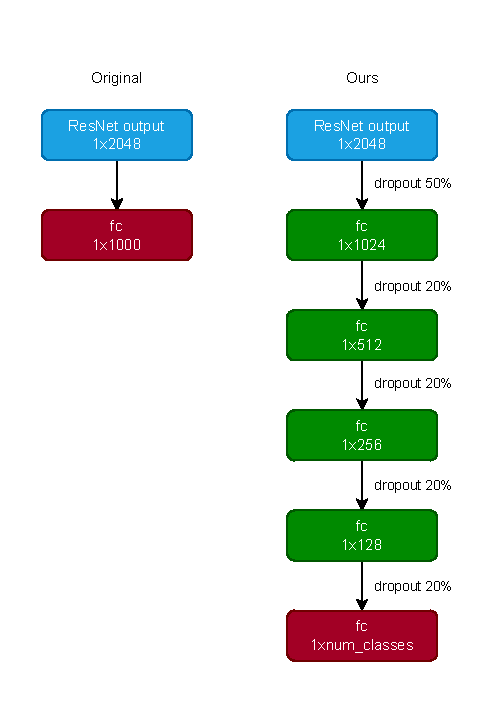
\includegraphics[width=0.6\textwidth]{figures/resnet_funnel.pdf}
      \caption{Our ResNet-50 architecture with a funnel layer for classification.
            Blue blocks represent the input from the ResNet-50 architecture,
            red blocks represent the final output layer,
            and green blocks represent our new funnel layers.}
      \label{fig:resnet_funnel}
\end{figure}

\subsubsection{Training Procedure}

In our initial training runs,
we observe severe overfitting on the training data as can be seen in Figure~\ref{fig:overfitting}.
To mitigate this, we apply several regularisation techniques:
\begin{itemize}
      \item \textbf{Dropout}~\cite{hinton_improving_2012}:
            As can be seen in Figure~\ref{fig:resnet_funnel},
            our fully connected layers contain dropout layers between them at rates of 0.5 and 0.2.
            Dropout is a regularisation technique that randomly sets a fraction of the input units to zero during training,
            which reinforces the model to learn more robust features and thereby reduces overfitting.
      \item \textbf{Data Augmentation}:
            We apply data augmentation techniques to our training data,
            such as random cropping, horizontal flipping, random erasing, and color jittering.
            These techniques artificially increase the size of our training dataset
            and help the model to generalise better by exposing it to a wider variety of input data.
\end{itemize}

\begin{figure}[ht]
      \centering
      \scalebox{0.6}{%% Creator: Matplotlib, PGF backend
%%
%% To include the figure in your LaTeX document, write
%%   \input{<filename>.pgf}
%%
%% Make sure the required packages are loaded in your preamble
%%   \usepackage{pgf}
%%
%% Also ensure that all the required font packages are loaded; for instance,
%% the lmodern package is sometimes necessary when using math font.
%%   \usepackage{lmodern}
%%
%% Figures using additional raster images can only be included by \input if
%% they are in the same directory as the main LaTeX file. For loading figures
%% from other directories you can use the `import` package
%%   \usepackage{import}
%%
%% and then include the figures with
%%   \import{<path to file>}{<filename>.pgf}
%%
%% Matplotlib used the following preamble
%%   \def\mathdefault#1{#1}
%%   \everymath=\expandafter{\the\everymath\displaystyle}
%%   \IfFileExists{scrextend.sty}{
%%     \usepackage[fontsize=11.000000pt]{scrextend}
%%   }{
%%     \renewcommand{\normalsize}{\fontsize{11.000000}{13.200000}\selectfont}
%%     \normalsize
%%   }
%%   
%%   \ifdefined\pdftexversion\else  % non-pdftex case.
%%     \usepackage{fontspec}
%%     \setmainfont{DejaVuSerif.ttf}[Path=\detokenize{/home/sentinel/.conda/envs/master-thesis/lib/python3.13/site-packages/matplotlib/mpl-data/fonts/ttf/}]
%%     \setsansfont{DejaVuSans.ttf}[Path=\detokenize{/home/sentinel/.conda/envs/master-thesis/lib/python3.13/site-packages/matplotlib/mpl-data/fonts/ttf/}]
%%     \setmonofont{DejaVuSansMono.ttf}[Path=\detokenize{/home/sentinel/.conda/envs/master-thesis/lib/python3.13/site-packages/matplotlib/mpl-data/fonts/ttf/}]
%%   \fi
%%   \makeatletter\@ifpackageloaded{underscore}{}{\usepackage[strings]{underscore}}\makeatother
%%
\begingroup%
\makeatletter%
\begin{pgfpicture}%
\pgfpathrectangle{\pgfpointorigin}{\pgfqpoint{5.344961in}{3.951110in}}%
\pgfusepath{use as bounding box, clip}%
\begin{pgfscope}%
\pgfsetbuttcap%
\pgfsetmiterjoin%
\definecolor{currentfill}{rgb}{1.000000,1.000000,1.000000}%
\pgfsetfillcolor{currentfill}%
\pgfsetlinewidth{0.000000pt}%
\definecolor{currentstroke}{rgb}{1.000000,1.000000,1.000000}%
\pgfsetstrokecolor{currentstroke}%
\pgfsetdash{}{0pt}%
\pgfpathmoveto{\pgfqpoint{0.000000in}{0.000000in}}%
\pgfpathlineto{\pgfqpoint{5.344961in}{0.000000in}}%
\pgfpathlineto{\pgfqpoint{5.344961in}{3.951110in}}%
\pgfpathlineto{\pgfqpoint{0.000000in}{3.951110in}}%
\pgfpathlineto{\pgfqpoint{0.000000in}{0.000000in}}%
\pgfpathclose%
\pgfusepath{fill}%
\end{pgfscope}%
\begin{pgfscope}%
\pgfsetbuttcap%
\pgfsetmiterjoin%
\definecolor{currentfill}{rgb}{1.000000,1.000000,1.000000}%
\pgfsetfillcolor{currentfill}%
\pgfsetlinewidth{0.000000pt}%
\definecolor{currentstroke}{rgb}{0.000000,0.000000,0.000000}%
\pgfsetstrokecolor{currentstroke}%
\pgfsetstrokeopacity{0.000000}%
\pgfsetdash{}{0pt}%
\pgfpathmoveto{\pgfqpoint{0.594961in}{0.548486in}}%
\pgfpathlineto{\pgfqpoint{5.244961in}{0.548486in}}%
\pgfpathlineto{\pgfqpoint{5.244961in}{3.628486in}}%
\pgfpathlineto{\pgfqpoint{0.594961in}{3.628486in}}%
\pgfpathlineto{\pgfqpoint{0.594961in}{0.548486in}}%
\pgfpathclose%
\pgfusepath{fill}%
\end{pgfscope}%
\begin{pgfscope}%
\pgfsetbuttcap%
\pgfsetroundjoin%
\definecolor{currentfill}{rgb}{0.000000,0.000000,0.000000}%
\pgfsetfillcolor{currentfill}%
\pgfsetlinewidth{0.803000pt}%
\definecolor{currentstroke}{rgb}{0.000000,0.000000,0.000000}%
\pgfsetstrokecolor{currentstroke}%
\pgfsetdash{}{0pt}%
\pgfsys@defobject{currentmarker}{\pgfqpoint{0.000000in}{-0.048611in}}{\pgfqpoint{0.000000in}{0.000000in}}{%
\pgfpathmoveto{\pgfqpoint{0.000000in}{0.000000in}}%
\pgfpathlineto{\pgfqpoint{0.000000in}{-0.048611in}}%
\pgfusepath{stroke,fill}%
}%
\begin{pgfscope}%
\pgfsys@transformshift{0.799717in}{0.548486in}%
\pgfsys@useobject{currentmarker}{}%
\end{pgfscope}%
\end{pgfscope}%
\begin{pgfscope}%
\definecolor{textcolor}{rgb}{0.000000,0.000000,0.000000}%
\pgfsetstrokecolor{textcolor}%
\pgfsetfillcolor{textcolor}%
\pgftext[x=0.799717in,y=0.451264in,,top]{\color{textcolor}{\fontsize{11.000000}{13.200000}\selectfont\catcode`\^=\active\def^{\ifmmode\sp\else\^{}\fi}\catcode`\%=\active\def%{\%}$\mathdefault{0}$}}%
\end{pgfscope}%
\begin{pgfscope}%
\pgfsetbuttcap%
\pgfsetroundjoin%
\definecolor{currentfill}{rgb}{0.000000,0.000000,0.000000}%
\pgfsetfillcolor{currentfill}%
\pgfsetlinewidth{0.803000pt}%
\definecolor{currentstroke}{rgb}{0.000000,0.000000,0.000000}%
\pgfsetstrokecolor{currentstroke}%
\pgfsetdash{}{0pt}%
\pgfsys@defobject{currentmarker}{\pgfqpoint{0.000000in}{-0.048611in}}{\pgfqpoint{0.000000in}{0.000000in}}{%
\pgfpathmoveto{\pgfqpoint{0.000000in}{0.000000in}}%
\pgfpathlineto{\pgfqpoint{0.000000in}{-0.048611in}}%
\pgfusepath{stroke,fill}%
}%
\begin{pgfscope}%
\pgfsys@transformshift{1.473924in}{0.548486in}%
\pgfsys@useobject{currentmarker}{}%
\end{pgfscope}%
\end{pgfscope}%
\begin{pgfscope}%
\definecolor{textcolor}{rgb}{0.000000,0.000000,0.000000}%
\pgfsetstrokecolor{textcolor}%
\pgfsetfillcolor{textcolor}%
\pgftext[x=1.473924in,y=0.451264in,,top]{\color{textcolor}{\fontsize{11.000000}{13.200000}\selectfont\catcode`\^=\active\def^{\ifmmode\sp\else\^{}\fi}\catcode`\%=\active\def%{\%}$\mathdefault{5000}$}}%
\end{pgfscope}%
\begin{pgfscope}%
\pgfsetbuttcap%
\pgfsetroundjoin%
\definecolor{currentfill}{rgb}{0.000000,0.000000,0.000000}%
\pgfsetfillcolor{currentfill}%
\pgfsetlinewidth{0.803000pt}%
\definecolor{currentstroke}{rgb}{0.000000,0.000000,0.000000}%
\pgfsetstrokecolor{currentstroke}%
\pgfsetdash{}{0pt}%
\pgfsys@defobject{currentmarker}{\pgfqpoint{0.000000in}{-0.048611in}}{\pgfqpoint{0.000000in}{0.000000in}}{%
\pgfpathmoveto{\pgfqpoint{0.000000in}{0.000000in}}%
\pgfpathlineto{\pgfqpoint{0.000000in}{-0.048611in}}%
\pgfusepath{stroke,fill}%
}%
\begin{pgfscope}%
\pgfsys@transformshift{2.148130in}{0.548486in}%
\pgfsys@useobject{currentmarker}{}%
\end{pgfscope}%
\end{pgfscope}%
\begin{pgfscope}%
\definecolor{textcolor}{rgb}{0.000000,0.000000,0.000000}%
\pgfsetstrokecolor{textcolor}%
\pgfsetfillcolor{textcolor}%
\pgftext[x=2.148130in,y=0.451264in,,top]{\color{textcolor}{\fontsize{11.000000}{13.200000}\selectfont\catcode`\^=\active\def^{\ifmmode\sp\else\^{}\fi}\catcode`\%=\active\def%{\%}$\mathdefault{10000}$}}%
\end{pgfscope}%
\begin{pgfscope}%
\pgfsetbuttcap%
\pgfsetroundjoin%
\definecolor{currentfill}{rgb}{0.000000,0.000000,0.000000}%
\pgfsetfillcolor{currentfill}%
\pgfsetlinewidth{0.803000pt}%
\definecolor{currentstroke}{rgb}{0.000000,0.000000,0.000000}%
\pgfsetstrokecolor{currentstroke}%
\pgfsetdash{}{0pt}%
\pgfsys@defobject{currentmarker}{\pgfqpoint{0.000000in}{-0.048611in}}{\pgfqpoint{0.000000in}{0.000000in}}{%
\pgfpathmoveto{\pgfqpoint{0.000000in}{0.000000in}}%
\pgfpathlineto{\pgfqpoint{0.000000in}{-0.048611in}}%
\pgfusepath{stroke,fill}%
}%
\begin{pgfscope}%
\pgfsys@transformshift{2.822336in}{0.548486in}%
\pgfsys@useobject{currentmarker}{}%
\end{pgfscope}%
\end{pgfscope}%
\begin{pgfscope}%
\definecolor{textcolor}{rgb}{0.000000,0.000000,0.000000}%
\pgfsetstrokecolor{textcolor}%
\pgfsetfillcolor{textcolor}%
\pgftext[x=2.822336in,y=0.451264in,,top]{\color{textcolor}{\fontsize{11.000000}{13.200000}\selectfont\catcode`\^=\active\def^{\ifmmode\sp\else\^{}\fi}\catcode`\%=\active\def%{\%}$\mathdefault{15000}$}}%
\end{pgfscope}%
\begin{pgfscope}%
\pgfsetbuttcap%
\pgfsetroundjoin%
\definecolor{currentfill}{rgb}{0.000000,0.000000,0.000000}%
\pgfsetfillcolor{currentfill}%
\pgfsetlinewidth{0.803000pt}%
\definecolor{currentstroke}{rgb}{0.000000,0.000000,0.000000}%
\pgfsetstrokecolor{currentstroke}%
\pgfsetdash{}{0pt}%
\pgfsys@defobject{currentmarker}{\pgfqpoint{0.000000in}{-0.048611in}}{\pgfqpoint{0.000000in}{0.000000in}}{%
\pgfpathmoveto{\pgfqpoint{0.000000in}{0.000000in}}%
\pgfpathlineto{\pgfqpoint{0.000000in}{-0.048611in}}%
\pgfusepath{stroke,fill}%
}%
\begin{pgfscope}%
\pgfsys@transformshift{3.496542in}{0.548486in}%
\pgfsys@useobject{currentmarker}{}%
\end{pgfscope}%
\end{pgfscope}%
\begin{pgfscope}%
\definecolor{textcolor}{rgb}{0.000000,0.000000,0.000000}%
\pgfsetstrokecolor{textcolor}%
\pgfsetfillcolor{textcolor}%
\pgftext[x=3.496542in,y=0.451264in,,top]{\color{textcolor}{\fontsize{11.000000}{13.200000}\selectfont\catcode`\^=\active\def^{\ifmmode\sp\else\^{}\fi}\catcode`\%=\active\def%{\%}$\mathdefault{20000}$}}%
\end{pgfscope}%
\begin{pgfscope}%
\pgfsetbuttcap%
\pgfsetroundjoin%
\definecolor{currentfill}{rgb}{0.000000,0.000000,0.000000}%
\pgfsetfillcolor{currentfill}%
\pgfsetlinewidth{0.803000pt}%
\definecolor{currentstroke}{rgb}{0.000000,0.000000,0.000000}%
\pgfsetstrokecolor{currentstroke}%
\pgfsetdash{}{0pt}%
\pgfsys@defobject{currentmarker}{\pgfqpoint{0.000000in}{-0.048611in}}{\pgfqpoint{0.000000in}{0.000000in}}{%
\pgfpathmoveto{\pgfqpoint{0.000000in}{0.000000in}}%
\pgfpathlineto{\pgfqpoint{0.000000in}{-0.048611in}}%
\pgfusepath{stroke,fill}%
}%
\begin{pgfscope}%
\pgfsys@transformshift{4.170748in}{0.548486in}%
\pgfsys@useobject{currentmarker}{}%
\end{pgfscope}%
\end{pgfscope}%
\begin{pgfscope}%
\definecolor{textcolor}{rgb}{0.000000,0.000000,0.000000}%
\pgfsetstrokecolor{textcolor}%
\pgfsetfillcolor{textcolor}%
\pgftext[x=4.170748in,y=0.451264in,,top]{\color{textcolor}{\fontsize{11.000000}{13.200000}\selectfont\catcode`\^=\active\def^{\ifmmode\sp\else\^{}\fi}\catcode`\%=\active\def%{\%}$\mathdefault{25000}$}}%
\end{pgfscope}%
\begin{pgfscope}%
\pgfsetbuttcap%
\pgfsetroundjoin%
\definecolor{currentfill}{rgb}{0.000000,0.000000,0.000000}%
\pgfsetfillcolor{currentfill}%
\pgfsetlinewidth{0.803000pt}%
\definecolor{currentstroke}{rgb}{0.000000,0.000000,0.000000}%
\pgfsetstrokecolor{currentstroke}%
\pgfsetdash{}{0pt}%
\pgfsys@defobject{currentmarker}{\pgfqpoint{0.000000in}{-0.048611in}}{\pgfqpoint{0.000000in}{0.000000in}}{%
\pgfpathmoveto{\pgfqpoint{0.000000in}{0.000000in}}%
\pgfpathlineto{\pgfqpoint{0.000000in}{-0.048611in}}%
\pgfusepath{stroke,fill}%
}%
\begin{pgfscope}%
\pgfsys@transformshift{4.844954in}{0.548486in}%
\pgfsys@useobject{currentmarker}{}%
\end{pgfscope}%
\end{pgfscope}%
\begin{pgfscope}%
\definecolor{textcolor}{rgb}{0.000000,0.000000,0.000000}%
\pgfsetstrokecolor{textcolor}%
\pgfsetfillcolor{textcolor}%
\pgftext[x=4.844954in,y=0.451264in,,top]{\color{textcolor}{\fontsize{11.000000}{13.200000}\selectfont\catcode`\^=\active\def^{\ifmmode\sp\else\^{}\fi}\catcode`\%=\active\def%{\%}$\mathdefault{30000}$}}%
\end{pgfscope}%
\begin{pgfscope}%
\definecolor{textcolor}{rgb}{0.000000,0.000000,0.000000}%
\pgfsetstrokecolor{textcolor}%
\pgfsetfillcolor{textcolor}%
\pgftext[x=2.919961in,y=0.247854in,,top]{\color{textcolor}{\fontsize{11.000000}{13.200000}\selectfont\catcode`\^=\active\def^{\ifmmode\sp\else\^{}\fi}\catcode`\%=\active\def%{\%}Steps}}%
\end{pgfscope}%
\begin{pgfscope}%
\pgfsetbuttcap%
\pgfsetroundjoin%
\definecolor{currentfill}{rgb}{0.000000,0.000000,0.000000}%
\pgfsetfillcolor{currentfill}%
\pgfsetlinewidth{0.803000pt}%
\definecolor{currentstroke}{rgb}{0.000000,0.000000,0.000000}%
\pgfsetstrokecolor{currentstroke}%
\pgfsetdash{}{0pt}%
\pgfsys@defobject{currentmarker}{\pgfqpoint{-0.048611in}{0.000000in}}{\pgfqpoint{-0.000000in}{0.000000in}}{%
\pgfpathmoveto{\pgfqpoint{-0.000000in}{0.000000in}}%
\pgfpathlineto{\pgfqpoint{-0.048611in}{0.000000in}}%
\pgfusepath{stroke,fill}%
}%
\begin{pgfscope}%
\pgfsys@transformshift{0.594961in}{0.688486in}%
\pgfsys@useobject{currentmarker}{}%
\end{pgfscope}%
\end{pgfscope}%
\begin{pgfscope}%
\definecolor{textcolor}{rgb}{0.000000,0.000000,0.000000}%
\pgfsetstrokecolor{textcolor}%
\pgfsetfillcolor{textcolor}%
\pgftext[x=0.303410in, y=0.630449in, left, base]{\color{textcolor}{\fontsize{11.000000}{13.200000}\selectfont\catcode`\^=\active\def^{\ifmmode\sp\else\^{}\fi}\catcode`\%=\active\def%{\%}$\mathdefault{0.0}$}}%
\end{pgfscope}%
\begin{pgfscope}%
\pgfsetbuttcap%
\pgfsetroundjoin%
\definecolor{currentfill}{rgb}{0.000000,0.000000,0.000000}%
\pgfsetfillcolor{currentfill}%
\pgfsetlinewidth{0.803000pt}%
\definecolor{currentstroke}{rgb}{0.000000,0.000000,0.000000}%
\pgfsetstrokecolor{currentstroke}%
\pgfsetdash{}{0pt}%
\pgfsys@defobject{currentmarker}{\pgfqpoint{-0.048611in}{0.000000in}}{\pgfqpoint{-0.000000in}{0.000000in}}{%
\pgfpathmoveto{\pgfqpoint{-0.000000in}{0.000000in}}%
\pgfpathlineto{\pgfqpoint{-0.048611in}{0.000000in}}%
\pgfusepath{stroke,fill}%
}%
\begin{pgfscope}%
\pgfsys@transformshift{0.594961in}{1.248486in}%
\pgfsys@useobject{currentmarker}{}%
\end{pgfscope}%
\end{pgfscope}%
\begin{pgfscope}%
\definecolor{textcolor}{rgb}{0.000000,0.000000,0.000000}%
\pgfsetstrokecolor{textcolor}%
\pgfsetfillcolor{textcolor}%
\pgftext[x=0.303410in, y=1.190449in, left, base]{\color{textcolor}{\fontsize{11.000000}{13.200000}\selectfont\catcode`\^=\active\def^{\ifmmode\sp\else\^{}\fi}\catcode`\%=\active\def%{\%}$\mathdefault{0.2}$}}%
\end{pgfscope}%
\begin{pgfscope}%
\pgfsetbuttcap%
\pgfsetroundjoin%
\definecolor{currentfill}{rgb}{0.000000,0.000000,0.000000}%
\pgfsetfillcolor{currentfill}%
\pgfsetlinewidth{0.803000pt}%
\definecolor{currentstroke}{rgb}{0.000000,0.000000,0.000000}%
\pgfsetstrokecolor{currentstroke}%
\pgfsetdash{}{0pt}%
\pgfsys@defobject{currentmarker}{\pgfqpoint{-0.048611in}{0.000000in}}{\pgfqpoint{-0.000000in}{0.000000in}}{%
\pgfpathmoveto{\pgfqpoint{-0.000000in}{0.000000in}}%
\pgfpathlineto{\pgfqpoint{-0.048611in}{0.000000in}}%
\pgfusepath{stroke,fill}%
}%
\begin{pgfscope}%
\pgfsys@transformshift{0.594961in}{1.808486in}%
\pgfsys@useobject{currentmarker}{}%
\end{pgfscope}%
\end{pgfscope}%
\begin{pgfscope}%
\definecolor{textcolor}{rgb}{0.000000,0.000000,0.000000}%
\pgfsetstrokecolor{textcolor}%
\pgfsetfillcolor{textcolor}%
\pgftext[x=0.303410in, y=1.750449in, left, base]{\color{textcolor}{\fontsize{11.000000}{13.200000}\selectfont\catcode`\^=\active\def^{\ifmmode\sp\else\^{}\fi}\catcode`\%=\active\def%{\%}$\mathdefault{0.4}$}}%
\end{pgfscope}%
\begin{pgfscope}%
\pgfsetbuttcap%
\pgfsetroundjoin%
\definecolor{currentfill}{rgb}{0.000000,0.000000,0.000000}%
\pgfsetfillcolor{currentfill}%
\pgfsetlinewidth{0.803000pt}%
\definecolor{currentstroke}{rgb}{0.000000,0.000000,0.000000}%
\pgfsetstrokecolor{currentstroke}%
\pgfsetdash{}{0pt}%
\pgfsys@defobject{currentmarker}{\pgfqpoint{-0.048611in}{0.000000in}}{\pgfqpoint{-0.000000in}{0.000000in}}{%
\pgfpathmoveto{\pgfqpoint{-0.000000in}{0.000000in}}%
\pgfpathlineto{\pgfqpoint{-0.048611in}{0.000000in}}%
\pgfusepath{stroke,fill}%
}%
\begin{pgfscope}%
\pgfsys@transformshift{0.594961in}{2.368486in}%
\pgfsys@useobject{currentmarker}{}%
\end{pgfscope}%
\end{pgfscope}%
\begin{pgfscope}%
\definecolor{textcolor}{rgb}{0.000000,0.000000,0.000000}%
\pgfsetstrokecolor{textcolor}%
\pgfsetfillcolor{textcolor}%
\pgftext[x=0.303410in, y=2.310449in, left, base]{\color{textcolor}{\fontsize{11.000000}{13.200000}\selectfont\catcode`\^=\active\def^{\ifmmode\sp\else\^{}\fi}\catcode`\%=\active\def%{\%}$\mathdefault{0.6}$}}%
\end{pgfscope}%
\begin{pgfscope}%
\pgfsetbuttcap%
\pgfsetroundjoin%
\definecolor{currentfill}{rgb}{0.000000,0.000000,0.000000}%
\pgfsetfillcolor{currentfill}%
\pgfsetlinewidth{0.803000pt}%
\definecolor{currentstroke}{rgb}{0.000000,0.000000,0.000000}%
\pgfsetstrokecolor{currentstroke}%
\pgfsetdash{}{0pt}%
\pgfsys@defobject{currentmarker}{\pgfqpoint{-0.048611in}{0.000000in}}{\pgfqpoint{-0.000000in}{0.000000in}}{%
\pgfpathmoveto{\pgfqpoint{-0.000000in}{0.000000in}}%
\pgfpathlineto{\pgfqpoint{-0.048611in}{0.000000in}}%
\pgfusepath{stroke,fill}%
}%
\begin{pgfscope}%
\pgfsys@transformshift{0.594961in}{2.928486in}%
\pgfsys@useobject{currentmarker}{}%
\end{pgfscope}%
\end{pgfscope}%
\begin{pgfscope}%
\definecolor{textcolor}{rgb}{0.000000,0.000000,0.000000}%
\pgfsetstrokecolor{textcolor}%
\pgfsetfillcolor{textcolor}%
\pgftext[x=0.303410in, y=2.870449in, left, base]{\color{textcolor}{\fontsize{11.000000}{13.200000}\selectfont\catcode`\^=\active\def^{\ifmmode\sp\else\^{}\fi}\catcode`\%=\active\def%{\%}$\mathdefault{0.8}$}}%
\end{pgfscope}%
\begin{pgfscope}%
\pgfsetbuttcap%
\pgfsetroundjoin%
\definecolor{currentfill}{rgb}{0.000000,0.000000,0.000000}%
\pgfsetfillcolor{currentfill}%
\pgfsetlinewidth{0.803000pt}%
\definecolor{currentstroke}{rgb}{0.000000,0.000000,0.000000}%
\pgfsetstrokecolor{currentstroke}%
\pgfsetdash{}{0pt}%
\pgfsys@defobject{currentmarker}{\pgfqpoint{-0.048611in}{0.000000in}}{\pgfqpoint{-0.000000in}{0.000000in}}{%
\pgfpathmoveto{\pgfqpoint{-0.000000in}{0.000000in}}%
\pgfpathlineto{\pgfqpoint{-0.048611in}{0.000000in}}%
\pgfusepath{stroke,fill}%
}%
\begin{pgfscope}%
\pgfsys@transformshift{0.594961in}{3.488486in}%
\pgfsys@useobject{currentmarker}{}%
\end{pgfscope}%
\end{pgfscope}%
\begin{pgfscope}%
\definecolor{textcolor}{rgb}{0.000000,0.000000,0.000000}%
\pgfsetstrokecolor{textcolor}%
\pgfsetfillcolor{textcolor}%
\pgftext[x=0.303410in, y=3.430449in, left, base]{\color{textcolor}{\fontsize{11.000000}{13.200000}\selectfont\catcode`\^=\active\def^{\ifmmode\sp\else\^{}\fi}\catcode`\%=\active\def%{\%}$\mathdefault{1.0}$}}%
\end{pgfscope}%
\begin{pgfscope}%
\definecolor{textcolor}{rgb}{0.000000,0.000000,0.000000}%
\pgfsetstrokecolor{textcolor}%
\pgfsetfillcolor{textcolor}%
\pgftext[x=0.247854in,y=2.088486in,,bottom,rotate=90.000000]{\color{textcolor}{\fontsize{11.000000}{13.200000}\selectfont\catcode`\^=\active\def^{\ifmmode\sp\else\^{}\fi}\catcode`\%=\active\def%{\%}Accuracy}}%
\end{pgfscope}%
\begin{pgfscope}%
\pgfpathrectangle{\pgfqpoint{0.594961in}{0.548486in}}{\pgfqpoint{4.650000in}{3.080000in}}%
\pgfusepath{clip}%
\pgfsetrectcap%
\pgfsetroundjoin%
\pgfsetlinewidth{1.505625pt}%
\definecolor{currentstroke}{rgb}{0.121569,0.466667,0.705882}%
\pgfsetstrokecolor{currentstroke}%
\pgfsetdash{}{0pt}%
\pgfpathmoveto{\pgfqpoint{0.806325in}{0.688486in}}%
\pgfpathlineto{\pgfqpoint{0.813067in}{0.754111in}}%
\pgfpathlineto{\pgfqpoint{0.819809in}{0.732236in}}%
\pgfpathlineto{\pgfqpoint{0.826551in}{0.765049in}}%
\pgfpathlineto{\pgfqpoint{0.833293in}{0.699424in}}%
\pgfpathlineto{\pgfqpoint{0.840035in}{0.721299in}}%
\pgfpathlineto{\pgfqpoint{0.846777in}{0.721299in}}%
\pgfpathlineto{\pgfqpoint{0.853519in}{0.699424in}}%
\pgfpathlineto{\pgfqpoint{0.860261in}{0.754111in}}%
\pgfpathlineto{\pgfqpoint{0.867003in}{0.721299in}}%
\pgfpathlineto{\pgfqpoint{0.873745in}{0.754111in}}%
\pgfpathlineto{\pgfqpoint{0.880487in}{0.743174in}}%
\pgfpathlineto{\pgfqpoint{0.887229in}{0.830674in}}%
\pgfpathlineto{\pgfqpoint{0.893971in}{0.797861in}}%
\pgfpathlineto{\pgfqpoint{0.900713in}{0.775986in}}%
\pgfpathlineto{\pgfqpoint{0.907456in}{0.797861in}}%
\pgfpathlineto{\pgfqpoint{0.914198in}{0.841611in}}%
\pgfpathlineto{\pgfqpoint{0.920940in}{0.819736in}}%
\pgfpathlineto{\pgfqpoint{0.927682in}{0.819736in}}%
\pgfpathlineto{\pgfqpoint{0.934424in}{0.885361in}}%
\pgfpathlineto{\pgfqpoint{0.941166in}{0.808799in}}%
\pgfpathlineto{\pgfqpoint{0.947908in}{0.797861in}}%
\pgfpathlineto{\pgfqpoint{0.954650in}{0.819736in}}%
\pgfpathlineto{\pgfqpoint{0.968134in}{0.797861in}}%
\pgfpathlineto{\pgfqpoint{0.974876in}{0.797861in}}%
\pgfpathlineto{\pgfqpoint{0.981618in}{0.852549in}}%
\pgfpathlineto{\pgfqpoint{0.988360in}{0.808799in}}%
\pgfpathlineto{\pgfqpoint{0.995102in}{0.863486in}}%
\pgfpathlineto{\pgfqpoint{1.001844in}{0.841611in}}%
\pgfpathlineto{\pgfqpoint{1.008586in}{0.940049in}}%
\pgfpathlineto{\pgfqpoint{1.015329in}{0.940049in}}%
\pgfpathlineto{\pgfqpoint{1.022071in}{1.016611in}}%
\pgfpathlineto{\pgfqpoint{1.028813in}{0.961924in}}%
\pgfpathlineto{\pgfqpoint{1.035555in}{0.950986in}}%
\pgfpathlineto{\pgfqpoint{1.042297in}{0.994736in}}%
\pgfpathlineto{\pgfqpoint{1.049039in}{0.940049in}}%
\pgfpathlineto{\pgfqpoint{1.055781in}{1.049424in}}%
\pgfpathlineto{\pgfqpoint{1.062523in}{1.060361in}}%
\pgfpathlineto{\pgfqpoint{1.069265in}{1.104111in}}%
\pgfpathlineto{\pgfqpoint{1.076007in}{0.950986in}}%
\pgfpathlineto{\pgfqpoint{1.082749in}{1.016611in}}%
\pgfpathlineto{\pgfqpoint{1.089491in}{1.071299in}}%
\pgfpathlineto{\pgfqpoint{1.096233in}{1.093174in}}%
\pgfpathlineto{\pgfqpoint{1.102975in}{1.180674in}}%
\pgfpathlineto{\pgfqpoint{1.109717in}{1.060361in}}%
\pgfpathlineto{\pgfqpoint{1.116459in}{1.136924in}}%
\pgfpathlineto{\pgfqpoint{1.129944in}{1.093174in}}%
\pgfpathlineto{\pgfqpoint{1.136686in}{1.093174in}}%
\pgfpathlineto{\pgfqpoint{1.143428in}{1.027549in}}%
\pgfpathlineto{\pgfqpoint{1.150170in}{1.136924in}}%
\pgfpathlineto{\pgfqpoint{1.156912in}{0.841611in}}%
\pgfpathlineto{\pgfqpoint{1.163654in}{1.125986in}}%
\pgfpathlineto{\pgfqpoint{1.170396in}{1.071299in}}%
\pgfpathlineto{\pgfqpoint{1.177138in}{1.213486in}}%
\pgfpathlineto{\pgfqpoint{1.183880in}{1.202549in}}%
\pgfpathlineto{\pgfqpoint{1.190622in}{1.300986in}}%
\pgfpathlineto{\pgfqpoint{1.197364in}{1.213486in}}%
\pgfpathlineto{\pgfqpoint{1.204106in}{1.224424in}}%
\pgfpathlineto{\pgfqpoint{1.210848in}{1.344736in}}%
\pgfpathlineto{\pgfqpoint{1.217590in}{1.377549in}}%
\pgfpathlineto{\pgfqpoint{1.224332in}{1.333799in}}%
\pgfpathlineto{\pgfqpoint{1.231074in}{1.443174in}}%
\pgfpathlineto{\pgfqpoint{1.237817in}{1.377549in}}%
\pgfpathlineto{\pgfqpoint{1.244559in}{1.355674in}}%
\pgfpathlineto{\pgfqpoint{1.251301in}{1.410361in}}%
\pgfpathlineto{\pgfqpoint{1.258043in}{1.388486in}}%
\pgfpathlineto{\pgfqpoint{1.264785in}{1.410361in}}%
\pgfpathlineto{\pgfqpoint{1.271527in}{1.486924in}}%
\pgfpathlineto{\pgfqpoint{1.278269in}{1.443174in}}%
\pgfpathlineto{\pgfqpoint{1.285011in}{1.574424in}}%
\pgfpathlineto{\pgfqpoint{1.291753in}{1.519736in}}%
\pgfpathlineto{\pgfqpoint{1.298495in}{1.629111in}}%
\pgfpathlineto{\pgfqpoint{1.305237in}{1.497861in}}%
\pgfpathlineto{\pgfqpoint{1.311979in}{1.618174in}}%
\pgfpathlineto{\pgfqpoint{1.318721in}{1.661924in}}%
\pgfpathlineto{\pgfqpoint{1.325463in}{1.475986in}}%
\pgfpathlineto{\pgfqpoint{1.332205in}{1.661924in}}%
\pgfpathlineto{\pgfqpoint{1.338947in}{1.530674in}}%
\pgfpathlineto{\pgfqpoint{1.345690in}{1.596299in}}%
\pgfpathlineto{\pgfqpoint{1.352432in}{1.574424in}}%
\pgfpathlineto{\pgfqpoint{1.359174in}{1.607236in}}%
\pgfpathlineto{\pgfqpoint{1.365916in}{1.705674in}}%
\pgfpathlineto{\pgfqpoint{1.372658in}{1.782236in}}%
\pgfpathlineto{\pgfqpoint{1.379400in}{1.541611in}}%
\pgfpathlineto{\pgfqpoint{1.392884in}{1.716611in}}%
\pgfpathlineto{\pgfqpoint{1.399626in}{1.771299in}}%
\pgfpathlineto{\pgfqpoint{1.406368in}{1.738486in}}%
\pgfpathlineto{\pgfqpoint{1.413110in}{1.596299in}}%
\pgfpathlineto{\pgfqpoint{1.419852in}{1.650986in}}%
\pgfpathlineto{\pgfqpoint{1.426594in}{1.880674in}}%
\pgfpathlineto{\pgfqpoint{1.433336in}{1.771299in}}%
\pgfpathlineto{\pgfqpoint{1.440078in}{1.858799in}}%
\pgfpathlineto{\pgfqpoint{1.446820in}{1.596299in}}%
\pgfpathlineto{\pgfqpoint{1.453563in}{1.705674in}}%
\pgfpathlineto{\pgfqpoint{1.467047in}{1.640049in}}%
\pgfpathlineto{\pgfqpoint{1.473789in}{1.902549in}}%
\pgfpathlineto{\pgfqpoint{1.480531in}{2.088486in}}%
\pgfpathlineto{\pgfqpoint{1.487273in}{1.869736in}}%
\pgfpathlineto{\pgfqpoint{1.494015in}{1.869736in}}%
\pgfpathlineto{\pgfqpoint{1.500757in}{1.847861in}}%
\pgfpathlineto{\pgfqpoint{1.507499in}{1.836924in}}%
\pgfpathlineto{\pgfqpoint{1.514241in}{2.077549in}}%
\pgfpathlineto{\pgfqpoint{1.520983in}{1.869736in}}%
\pgfpathlineto{\pgfqpoint{1.527725in}{1.979111in}}%
\pgfpathlineto{\pgfqpoint{1.534467in}{2.000986in}}%
\pgfpathlineto{\pgfqpoint{1.541209in}{2.044736in}}%
\pgfpathlineto{\pgfqpoint{1.547951in}{1.858799in}}%
\pgfpathlineto{\pgfqpoint{1.554693in}{1.891611in}}%
\pgfpathlineto{\pgfqpoint{1.561436in}{2.077549in}}%
\pgfpathlineto{\pgfqpoint{1.568178in}{1.990049in}}%
\pgfpathlineto{\pgfqpoint{1.574920in}{1.836924in}}%
\pgfpathlineto{\pgfqpoint{1.581662in}{1.541611in}}%
\pgfpathlineto{\pgfqpoint{1.588404in}{1.935361in}}%
\pgfpathlineto{\pgfqpoint{1.595146in}{1.946299in}}%
\pgfpathlineto{\pgfqpoint{1.601888in}{2.066611in}}%
\pgfpathlineto{\pgfqpoint{1.608630in}{1.935361in}}%
\pgfpathlineto{\pgfqpoint{1.615372in}{1.902549in}}%
\pgfpathlineto{\pgfqpoint{1.622114in}{2.219736in}}%
\pgfpathlineto{\pgfqpoint{1.628856in}{2.055674in}}%
\pgfpathlineto{\pgfqpoint{1.635598in}{2.066611in}}%
\pgfpathlineto{\pgfqpoint{1.642340in}{2.099424in}}%
\pgfpathlineto{\pgfqpoint{1.649082in}{2.263486in}}%
\pgfpathlineto{\pgfqpoint{1.655824in}{2.110361in}}%
\pgfpathlineto{\pgfqpoint{1.662566in}{2.044736in}}%
\pgfpathlineto{\pgfqpoint{1.669309in}{2.175986in}}%
\pgfpathlineto{\pgfqpoint{1.676051in}{2.186924in}}%
\pgfpathlineto{\pgfqpoint{1.682793in}{2.186924in}}%
\pgfpathlineto{\pgfqpoint{1.689535in}{2.252549in}}%
\pgfpathlineto{\pgfqpoint{1.696277in}{2.132236in}}%
\pgfpathlineto{\pgfqpoint{1.703019in}{2.241611in}}%
\pgfpathlineto{\pgfqpoint{1.709761in}{2.022861in}}%
\pgfpathlineto{\pgfqpoint{1.716503in}{2.197861in}}%
\pgfpathlineto{\pgfqpoint{1.723245in}{2.099424in}}%
\pgfpathlineto{\pgfqpoint{1.729987in}{2.252549in}}%
\pgfpathlineto{\pgfqpoint{1.736729in}{2.121299in}}%
\pgfpathlineto{\pgfqpoint{1.743471in}{2.296299in}}%
\pgfpathlineto{\pgfqpoint{1.750213in}{2.165049in}}%
\pgfpathlineto{\pgfqpoint{1.763697in}{2.252549in}}%
\pgfpathlineto{\pgfqpoint{1.770439in}{2.219736in}}%
\pgfpathlineto{\pgfqpoint{1.777182in}{2.416611in}}%
\pgfpathlineto{\pgfqpoint{1.783924in}{2.208799in}}%
\pgfpathlineto{\pgfqpoint{1.790666in}{2.427549in}}%
\pgfpathlineto{\pgfqpoint{1.797408in}{2.296299in}}%
\pgfpathlineto{\pgfqpoint{1.804150in}{2.536924in}}%
\pgfpathlineto{\pgfqpoint{1.810892in}{2.383799in}}%
\pgfpathlineto{\pgfqpoint{1.817634in}{2.416611in}}%
\pgfpathlineto{\pgfqpoint{1.824376in}{2.219736in}}%
\pgfpathlineto{\pgfqpoint{1.831118in}{2.252549in}}%
\pgfpathlineto{\pgfqpoint{1.837860in}{2.329111in}}%
\pgfpathlineto{\pgfqpoint{1.844602in}{2.318174in}}%
\pgfpathlineto{\pgfqpoint{1.851344in}{2.536924in}}%
\pgfpathlineto{\pgfqpoint{1.858086in}{3.138486in}}%
\pgfpathlineto{\pgfqpoint{1.864828in}{2.394736in}}%
\pgfpathlineto{\pgfqpoint{1.871570in}{2.679111in}}%
\pgfpathlineto{\pgfqpoint{1.878312in}{2.613486in}}%
\pgfpathlineto{\pgfqpoint{1.885054in}{2.558799in}}%
\pgfpathlineto{\pgfqpoint{1.891797in}{2.449424in}}%
\pgfpathlineto{\pgfqpoint{1.898539in}{2.438486in}}%
\pgfpathlineto{\pgfqpoint{1.905281in}{2.624424in}}%
\pgfpathlineto{\pgfqpoint{1.912023in}{2.427549in}}%
\pgfpathlineto{\pgfqpoint{1.918765in}{2.493174in}}%
\pgfpathlineto{\pgfqpoint{1.925507in}{2.427549in}}%
\pgfpathlineto{\pgfqpoint{1.932249in}{2.449424in}}%
\pgfpathlineto{\pgfqpoint{1.938991in}{2.580674in}}%
\pgfpathlineto{\pgfqpoint{1.945733in}{2.536924in}}%
\pgfpathlineto{\pgfqpoint{1.952475in}{2.482236in}}%
\pgfpathlineto{\pgfqpoint{1.959217in}{2.493174in}}%
\pgfpathlineto{\pgfqpoint{1.965959in}{2.405674in}}%
\pgfpathlineto{\pgfqpoint{1.972701in}{2.504111in}}%
\pgfpathlineto{\pgfqpoint{1.979443in}{2.525986in}}%
\pgfpathlineto{\pgfqpoint{1.986185in}{2.525986in}}%
\pgfpathlineto{\pgfqpoint{1.992927in}{2.493174in}}%
\pgfpathlineto{\pgfqpoint{1.999670in}{2.613486in}}%
\pgfpathlineto{\pgfqpoint{2.006412in}{2.471299in}}%
\pgfpathlineto{\pgfqpoint{2.013154in}{2.515049in}}%
\pgfpathlineto{\pgfqpoint{2.019896in}{2.471299in}}%
\pgfpathlineto{\pgfqpoint{2.026638in}{2.624424in}}%
\pgfpathlineto{\pgfqpoint{2.033380in}{2.350986in}}%
\pgfpathlineto{\pgfqpoint{2.040122in}{2.525986in}}%
\pgfpathlineto{\pgfqpoint{2.046864in}{2.536924in}}%
\pgfpathlineto{\pgfqpoint{2.053606in}{2.635361in}}%
\pgfpathlineto{\pgfqpoint{2.060348in}{2.536924in}}%
\pgfpathlineto{\pgfqpoint{2.067090in}{2.602549in}}%
\pgfpathlineto{\pgfqpoint{2.073832in}{2.646299in}}%
\pgfpathlineto{\pgfqpoint{2.080574in}{2.952549in}}%
\pgfpathlineto{\pgfqpoint{2.087316in}{3.204111in}}%
\pgfpathlineto{\pgfqpoint{2.094058in}{3.061924in}}%
\pgfpathlineto{\pgfqpoint{2.100800in}{3.061924in}}%
\pgfpathlineto{\pgfqpoint{2.107543in}{3.204111in}}%
\pgfpathlineto{\pgfqpoint{2.114285in}{3.138486in}}%
\pgfpathlineto{\pgfqpoint{2.121027in}{3.225986in}}%
\pgfpathlineto{\pgfqpoint{2.127769in}{3.149424in}}%
\pgfpathlineto{\pgfqpoint{2.134511in}{3.204111in}}%
\pgfpathlineto{\pgfqpoint{2.141253in}{3.204111in}}%
\pgfpathlineto{\pgfqpoint{2.147995in}{3.225986in}}%
\pgfpathlineto{\pgfqpoint{2.154737in}{3.302549in}}%
\pgfpathlineto{\pgfqpoint{2.161479in}{3.269736in}}%
\pgfpathlineto{\pgfqpoint{2.168221in}{3.269736in}}%
\pgfpathlineto{\pgfqpoint{2.174963in}{3.236924in}}%
\pgfpathlineto{\pgfqpoint{2.181705in}{3.357236in}}%
\pgfpathlineto{\pgfqpoint{2.188447in}{3.335361in}}%
\pgfpathlineto{\pgfqpoint{2.195189in}{3.411924in}}%
\pgfpathlineto{\pgfqpoint{2.201931in}{3.390049in}}%
\pgfpathlineto{\pgfqpoint{2.208673in}{3.324424in}}%
\pgfpathlineto{\pgfqpoint{2.215416in}{3.400986in}}%
\pgfpathlineto{\pgfqpoint{2.222158in}{3.346299in}}%
\pgfpathlineto{\pgfqpoint{2.228900in}{3.400986in}}%
\pgfpathlineto{\pgfqpoint{2.235642in}{3.357236in}}%
\pgfpathlineto{\pgfqpoint{2.249126in}{3.291611in}}%
\pgfpathlineto{\pgfqpoint{2.255868in}{3.390049in}}%
\pgfpathlineto{\pgfqpoint{2.262610in}{3.357236in}}%
\pgfpathlineto{\pgfqpoint{2.269352in}{3.390049in}}%
\pgfpathlineto{\pgfqpoint{2.276094in}{3.346299in}}%
\pgfpathlineto{\pgfqpoint{2.282836in}{3.400986in}}%
\pgfpathlineto{\pgfqpoint{2.289578in}{3.357236in}}%
\pgfpathlineto{\pgfqpoint{2.296320in}{3.422861in}}%
\pgfpathlineto{\pgfqpoint{2.303062in}{3.379111in}}%
\pgfpathlineto{\pgfqpoint{2.309804in}{3.422861in}}%
\pgfpathlineto{\pgfqpoint{2.316546in}{3.313486in}}%
\pgfpathlineto{\pgfqpoint{2.323289in}{3.357236in}}%
\pgfpathlineto{\pgfqpoint{2.330031in}{3.357236in}}%
\pgfpathlineto{\pgfqpoint{2.336773in}{3.455674in}}%
\pgfpathlineto{\pgfqpoint{2.343515in}{3.335361in}}%
\pgfpathlineto{\pgfqpoint{2.350257in}{3.422861in}}%
\pgfpathlineto{\pgfqpoint{2.356999in}{3.357236in}}%
\pgfpathlineto{\pgfqpoint{2.363741in}{3.422861in}}%
\pgfpathlineto{\pgfqpoint{2.370483in}{3.411924in}}%
\pgfpathlineto{\pgfqpoint{2.377225in}{3.368174in}}%
\pgfpathlineto{\pgfqpoint{2.383967in}{3.346299in}}%
\pgfpathlineto{\pgfqpoint{2.390709in}{3.411924in}}%
\pgfpathlineto{\pgfqpoint{2.397451in}{3.379111in}}%
\pgfpathlineto{\pgfqpoint{2.404193in}{3.390049in}}%
\pgfpathlineto{\pgfqpoint{2.417677in}{3.433799in}}%
\pgfpathlineto{\pgfqpoint{2.424419in}{3.400986in}}%
\pgfpathlineto{\pgfqpoint{2.431161in}{3.379111in}}%
\pgfpathlineto{\pgfqpoint{2.437904in}{3.346299in}}%
\pgfpathlineto{\pgfqpoint{2.444646in}{3.411924in}}%
\pgfpathlineto{\pgfqpoint{2.458130in}{3.368174in}}%
\pgfpathlineto{\pgfqpoint{2.464872in}{3.422861in}}%
\pgfpathlineto{\pgfqpoint{2.471614in}{3.390049in}}%
\pgfpathlineto{\pgfqpoint{2.478356in}{3.324424in}}%
\pgfpathlineto{\pgfqpoint{2.485098in}{3.422861in}}%
\pgfpathlineto{\pgfqpoint{2.491840in}{3.368174in}}%
\pgfpathlineto{\pgfqpoint{2.498582in}{3.411924in}}%
\pgfpathlineto{\pgfqpoint{2.505324in}{3.390049in}}%
\pgfpathlineto{\pgfqpoint{2.512066in}{3.335361in}}%
\pgfpathlineto{\pgfqpoint{2.518808in}{3.379111in}}%
\pgfpathlineto{\pgfqpoint{2.525550in}{3.411924in}}%
\pgfpathlineto{\pgfqpoint{2.532292in}{3.346299in}}%
\pgfpathlineto{\pgfqpoint{2.539034in}{3.390049in}}%
\pgfpathlineto{\pgfqpoint{2.545777in}{3.346299in}}%
\pgfpathlineto{\pgfqpoint{2.552519in}{3.324424in}}%
\pgfpathlineto{\pgfqpoint{2.559261in}{3.390049in}}%
\pgfpathlineto{\pgfqpoint{2.566003in}{3.357236in}}%
\pgfpathlineto{\pgfqpoint{2.572745in}{3.433799in}}%
\pgfpathlineto{\pgfqpoint{2.579487in}{3.357236in}}%
\pgfpathlineto{\pgfqpoint{2.586229in}{3.357236in}}%
\pgfpathlineto{\pgfqpoint{2.592971in}{3.368174in}}%
\pgfpathlineto{\pgfqpoint{2.599713in}{3.422861in}}%
\pgfpathlineto{\pgfqpoint{2.606455in}{3.433799in}}%
\pgfpathlineto{\pgfqpoint{2.619939in}{3.411924in}}%
\pgfpathlineto{\pgfqpoint{2.626681in}{3.368174in}}%
\pgfpathlineto{\pgfqpoint{2.633423in}{3.400986in}}%
\pgfpathlineto{\pgfqpoint{2.640165in}{3.335361in}}%
\pgfpathlineto{\pgfqpoint{2.646907in}{3.390049in}}%
\pgfpathlineto{\pgfqpoint{2.653650in}{3.422861in}}%
\pgfpathlineto{\pgfqpoint{2.660392in}{3.302549in}}%
\pgfpathlineto{\pgfqpoint{2.667134in}{3.335361in}}%
\pgfpathlineto{\pgfqpoint{2.673876in}{3.335361in}}%
\pgfpathlineto{\pgfqpoint{2.680618in}{3.357236in}}%
\pgfpathlineto{\pgfqpoint{2.687360in}{3.335361in}}%
\pgfpathlineto{\pgfqpoint{2.694102in}{3.422861in}}%
\pgfpathlineto{\pgfqpoint{2.700844in}{3.335361in}}%
\pgfpathlineto{\pgfqpoint{2.707586in}{3.357236in}}%
\pgfpathlineto{\pgfqpoint{2.714328in}{3.400986in}}%
\pgfpathlineto{\pgfqpoint{2.721070in}{3.422861in}}%
\pgfpathlineto{\pgfqpoint{2.727812in}{3.411924in}}%
\pgfpathlineto{\pgfqpoint{2.734554in}{3.346299in}}%
\pgfpathlineto{\pgfqpoint{2.741296in}{3.368174in}}%
\pgfpathlineto{\pgfqpoint{2.748038in}{3.346299in}}%
\pgfpathlineto{\pgfqpoint{2.754780in}{3.357236in}}%
\pgfpathlineto{\pgfqpoint{2.761523in}{3.335361in}}%
\pgfpathlineto{\pgfqpoint{2.768265in}{3.379111in}}%
\pgfpathlineto{\pgfqpoint{2.775007in}{3.291611in}}%
\pgfpathlineto{\pgfqpoint{2.781749in}{3.324424in}}%
\pgfpathlineto{\pgfqpoint{2.788491in}{3.313486in}}%
\pgfpathlineto{\pgfqpoint{2.795233in}{3.379111in}}%
\pgfpathlineto{\pgfqpoint{2.801975in}{3.357236in}}%
\pgfpathlineto{\pgfqpoint{2.808717in}{3.269736in}}%
\pgfpathlineto{\pgfqpoint{2.815459in}{3.346299in}}%
\pgfpathlineto{\pgfqpoint{2.822201in}{3.324424in}}%
\pgfpathlineto{\pgfqpoint{2.828943in}{3.324424in}}%
\pgfpathlineto{\pgfqpoint{2.835685in}{3.422861in}}%
\pgfpathlineto{\pgfqpoint{2.842427in}{3.269736in}}%
\pgfpathlineto{\pgfqpoint{2.849169in}{3.368174in}}%
\pgfpathlineto{\pgfqpoint{2.855911in}{3.335361in}}%
\pgfpathlineto{\pgfqpoint{2.862653in}{3.335361in}}%
\pgfpathlineto{\pgfqpoint{2.876138in}{3.379111in}}%
\pgfpathlineto{\pgfqpoint{2.882880in}{3.357236in}}%
\pgfpathlineto{\pgfqpoint{2.889622in}{3.346299in}}%
\pgfpathlineto{\pgfqpoint{2.896364in}{3.313486in}}%
\pgfpathlineto{\pgfqpoint{2.909848in}{3.313486in}}%
\pgfpathlineto{\pgfqpoint{2.916590in}{3.488486in}}%
\pgfpathlineto{\pgfqpoint{2.923332in}{3.302549in}}%
\pgfpathlineto{\pgfqpoint{2.930074in}{3.379111in}}%
\pgfpathlineto{\pgfqpoint{2.936816in}{3.357236in}}%
\pgfpathlineto{\pgfqpoint{2.943558in}{3.368174in}}%
\pgfpathlineto{\pgfqpoint{2.950300in}{3.400986in}}%
\pgfpathlineto{\pgfqpoint{2.957042in}{3.357236in}}%
\pgfpathlineto{\pgfqpoint{2.970526in}{3.313486in}}%
\pgfpathlineto{\pgfqpoint{2.977268in}{3.379111in}}%
\pgfpathlineto{\pgfqpoint{2.984011in}{3.379111in}}%
\pgfpathlineto{\pgfqpoint{2.990753in}{3.346299in}}%
\pgfpathlineto{\pgfqpoint{2.997495in}{3.368174in}}%
\pgfpathlineto{\pgfqpoint{3.004237in}{3.379111in}}%
\pgfpathlineto{\pgfqpoint{3.010979in}{3.400986in}}%
\pgfpathlineto{\pgfqpoint{3.024463in}{3.335361in}}%
\pgfpathlineto{\pgfqpoint{3.031205in}{3.324424in}}%
\pgfpathlineto{\pgfqpoint{3.037947in}{3.346299in}}%
\pgfpathlineto{\pgfqpoint{3.044689in}{3.357236in}}%
\pgfpathlineto{\pgfqpoint{3.051431in}{3.324424in}}%
\pgfpathlineto{\pgfqpoint{3.058173in}{3.390049in}}%
\pgfpathlineto{\pgfqpoint{3.064915in}{3.346299in}}%
\pgfpathlineto{\pgfqpoint{3.071657in}{3.291611in}}%
\pgfpathlineto{\pgfqpoint{3.078399in}{3.357236in}}%
\pgfpathlineto{\pgfqpoint{3.085141in}{3.400986in}}%
\pgfpathlineto{\pgfqpoint{3.091884in}{3.258799in}}%
\pgfpathlineto{\pgfqpoint{3.105368in}{3.444736in}}%
\pgfpathlineto{\pgfqpoint{3.112110in}{3.368174in}}%
\pgfpathlineto{\pgfqpoint{3.118852in}{3.313486in}}%
\pgfpathlineto{\pgfqpoint{3.125594in}{3.313486in}}%
\pgfpathlineto{\pgfqpoint{3.132336in}{3.346299in}}%
\pgfpathlineto{\pgfqpoint{3.139078in}{3.335361in}}%
\pgfpathlineto{\pgfqpoint{3.145820in}{3.346299in}}%
\pgfpathlineto{\pgfqpoint{3.152562in}{3.313486in}}%
\pgfpathlineto{\pgfqpoint{3.159304in}{3.346299in}}%
\pgfpathlineto{\pgfqpoint{3.166046in}{3.390049in}}%
\pgfpathlineto{\pgfqpoint{3.172788in}{3.368174in}}%
\pgfpathlineto{\pgfqpoint{3.179530in}{3.357236in}}%
\pgfpathlineto{\pgfqpoint{3.186272in}{3.291611in}}%
\pgfpathlineto{\pgfqpoint{3.193014in}{3.280674in}}%
\pgfpathlineto{\pgfqpoint{3.199757in}{3.313486in}}%
\pgfpathlineto{\pgfqpoint{3.206499in}{3.411924in}}%
\pgfpathlineto{\pgfqpoint{3.213241in}{3.291611in}}%
\pgfpathlineto{\pgfqpoint{3.219983in}{3.390049in}}%
\pgfpathlineto{\pgfqpoint{3.226725in}{3.313486in}}%
\pgfpathlineto{\pgfqpoint{3.233467in}{3.335361in}}%
\pgfpathlineto{\pgfqpoint{3.260435in}{3.335361in}}%
\pgfpathlineto{\pgfqpoint{3.267177in}{3.291611in}}%
\pgfpathlineto{\pgfqpoint{3.273919in}{3.335361in}}%
\pgfpathlineto{\pgfqpoint{3.280661in}{3.357236in}}%
\pgfpathlineto{\pgfqpoint{3.287403in}{3.335361in}}%
\pgfpathlineto{\pgfqpoint{3.294145in}{3.346299in}}%
\pgfpathlineto{\pgfqpoint{3.300887in}{3.379111in}}%
\pgfpathlineto{\pgfqpoint{3.307630in}{3.400986in}}%
\pgfpathlineto{\pgfqpoint{3.314372in}{3.335361in}}%
\pgfpathlineto{\pgfqpoint{3.321114in}{3.335361in}}%
\pgfpathlineto{\pgfqpoint{3.327856in}{3.346299in}}%
\pgfpathlineto{\pgfqpoint{3.334598in}{3.390049in}}%
\pgfpathlineto{\pgfqpoint{3.348082in}{3.433799in}}%
\pgfpathlineto{\pgfqpoint{3.354824in}{3.433799in}}%
\pgfpathlineto{\pgfqpoint{3.361566in}{3.455674in}}%
\pgfpathlineto{\pgfqpoint{3.375050in}{3.455674in}}%
\pgfpathlineto{\pgfqpoint{3.381792in}{3.466611in}}%
\pgfpathlineto{\pgfqpoint{3.388534in}{3.455674in}}%
\pgfpathlineto{\pgfqpoint{3.395276in}{3.488486in}}%
\pgfpathlineto{\pgfqpoint{3.402018in}{3.488486in}}%
\pgfpathlineto{\pgfqpoint{3.408760in}{3.444736in}}%
\pgfpathlineto{\pgfqpoint{3.415503in}{3.477549in}}%
\pgfpathlineto{\pgfqpoint{3.422245in}{3.444736in}}%
\pgfpathlineto{\pgfqpoint{3.428987in}{3.477549in}}%
\pgfpathlineto{\pgfqpoint{3.435729in}{3.488486in}}%
\pgfpathlineto{\pgfqpoint{3.442471in}{3.466611in}}%
\pgfpathlineto{\pgfqpoint{3.449213in}{3.455674in}}%
\pgfpathlineto{\pgfqpoint{3.455955in}{3.488486in}}%
\pgfpathlineto{\pgfqpoint{3.462697in}{3.455674in}}%
\pgfpathlineto{\pgfqpoint{3.469439in}{3.455674in}}%
\pgfpathlineto{\pgfqpoint{3.476181in}{3.466611in}}%
\pgfpathlineto{\pgfqpoint{3.482923in}{3.488486in}}%
\pgfpathlineto{\pgfqpoint{3.489665in}{3.466611in}}%
\pgfpathlineto{\pgfqpoint{3.503149in}{3.466611in}}%
\pgfpathlineto{\pgfqpoint{3.509891in}{3.488486in}}%
\pgfpathlineto{\pgfqpoint{3.516633in}{3.444736in}}%
\pgfpathlineto{\pgfqpoint{3.543602in}{3.488486in}}%
\pgfpathlineto{\pgfqpoint{3.550344in}{3.488486in}}%
\pgfpathlineto{\pgfqpoint{3.557086in}{3.477549in}}%
\pgfpathlineto{\pgfqpoint{3.563828in}{3.477549in}}%
\pgfpathlineto{\pgfqpoint{3.570570in}{3.488486in}}%
\pgfpathlineto{\pgfqpoint{3.577312in}{3.477549in}}%
\pgfpathlineto{\pgfqpoint{3.584054in}{3.488486in}}%
\pgfpathlineto{\pgfqpoint{3.590796in}{3.466611in}}%
\pgfpathlineto{\pgfqpoint{3.597538in}{3.477549in}}%
\pgfpathlineto{\pgfqpoint{3.604280in}{3.466611in}}%
\pgfpathlineto{\pgfqpoint{3.611022in}{3.488486in}}%
\pgfpathlineto{\pgfqpoint{3.617764in}{3.477549in}}%
\pgfpathlineto{\pgfqpoint{3.624506in}{3.477549in}}%
\pgfpathlineto{\pgfqpoint{3.631248in}{3.488486in}}%
\pgfpathlineto{\pgfqpoint{3.637991in}{3.477549in}}%
\pgfpathlineto{\pgfqpoint{3.644733in}{3.477549in}}%
\pgfpathlineto{\pgfqpoint{3.651475in}{3.488486in}}%
\pgfpathlineto{\pgfqpoint{3.658217in}{3.455674in}}%
\pgfpathlineto{\pgfqpoint{3.664959in}{3.477549in}}%
\pgfpathlineto{\pgfqpoint{3.671701in}{3.466611in}}%
\pgfpathlineto{\pgfqpoint{3.678443in}{3.488486in}}%
\pgfpathlineto{\pgfqpoint{3.698669in}{3.488486in}}%
\pgfpathlineto{\pgfqpoint{3.705411in}{3.455674in}}%
\pgfpathlineto{\pgfqpoint{3.712153in}{3.466611in}}%
\pgfpathlineto{\pgfqpoint{3.718895in}{3.488486in}}%
\pgfpathlineto{\pgfqpoint{3.725637in}{3.477549in}}%
\pgfpathlineto{\pgfqpoint{3.739121in}{3.477549in}}%
\pgfpathlineto{\pgfqpoint{3.745864in}{3.488486in}}%
\pgfpathlineto{\pgfqpoint{3.759348in}{3.466611in}}%
\pgfpathlineto{\pgfqpoint{3.766090in}{3.488486in}}%
\pgfpathlineto{\pgfqpoint{3.772832in}{3.488486in}}%
\pgfpathlineto{\pgfqpoint{3.779574in}{3.477549in}}%
\pgfpathlineto{\pgfqpoint{3.786316in}{3.477549in}}%
\pgfpathlineto{\pgfqpoint{3.793058in}{3.466611in}}%
\pgfpathlineto{\pgfqpoint{3.799800in}{3.477549in}}%
\pgfpathlineto{\pgfqpoint{3.813284in}{3.477549in}}%
\pgfpathlineto{\pgfqpoint{3.820026in}{3.488486in}}%
\pgfpathlineto{\pgfqpoint{3.826768in}{3.488486in}}%
\pgfpathlineto{\pgfqpoint{3.833510in}{3.477549in}}%
\pgfpathlineto{\pgfqpoint{3.840252in}{3.488486in}}%
\pgfpathlineto{\pgfqpoint{3.873963in}{3.488486in}}%
\pgfpathlineto{\pgfqpoint{3.880705in}{3.477549in}}%
\pgfpathlineto{\pgfqpoint{3.887447in}{3.488486in}}%
\pgfpathlineto{\pgfqpoint{3.900931in}{3.488486in}}%
\pgfpathlineto{\pgfqpoint{3.907673in}{3.477549in}}%
\pgfpathlineto{\pgfqpoint{3.914415in}{3.488486in}}%
\pgfpathlineto{\pgfqpoint{3.921157in}{3.477549in}}%
\pgfpathlineto{\pgfqpoint{3.927899in}{3.488486in}}%
\pgfpathlineto{\pgfqpoint{3.934641in}{3.477549in}}%
\pgfpathlineto{\pgfqpoint{3.941383in}{3.477549in}}%
\pgfpathlineto{\pgfqpoint{3.948125in}{3.488486in}}%
\pgfpathlineto{\pgfqpoint{3.954867in}{3.477549in}}%
\pgfpathlineto{\pgfqpoint{3.961610in}{3.488486in}}%
\pgfpathlineto{\pgfqpoint{3.968352in}{3.477549in}}%
\pgfpathlineto{\pgfqpoint{3.975094in}{3.488486in}}%
\pgfpathlineto{\pgfqpoint{4.002062in}{3.488486in}}%
\pgfpathlineto{\pgfqpoint{4.008804in}{3.477549in}}%
\pgfpathlineto{\pgfqpoint{4.015546in}{3.488486in}}%
\pgfpathlineto{\pgfqpoint{4.022288in}{3.488486in}}%
\pgfpathlineto{\pgfqpoint{4.029030in}{3.477549in}}%
\pgfpathlineto{\pgfqpoint{4.035772in}{3.488486in}}%
\pgfpathlineto{\pgfqpoint{4.042514in}{3.488486in}}%
\pgfpathlineto{\pgfqpoint{4.049256in}{3.477549in}}%
\pgfpathlineto{\pgfqpoint{4.055998in}{3.488486in}}%
\pgfpathlineto{\pgfqpoint{4.062740in}{3.488486in}}%
\pgfpathlineto{\pgfqpoint{4.069483in}{3.477549in}}%
\pgfpathlineto{\pgfqpoint{4.076225in}{3.488486in}}%
\pgfpathlineto{\pgfqpoint{4.103193in}{3.488486in}}%
\pgfpathlineto{\pgfqpoint{4.109935in}{3.477549in}}%
\pgfpathlineto{\pgfqpoint{4.116677in}{3.477549in}}%
\pgfpathlineto{\pgfqpoint{4.123419in}{3.488486in}}%
\pgfpathlineto{\pgfqpoint{4.130161in}{3.477549in}}%
\pgfpathlineto{\pgfqpoint{4.136903in}{3.488486in}}%
\pgfpathlineto{\pgfqpoint{4.143645in}{3.477549in}}%
\pgfpathlineto{\pgfqpoint{4.150387in}{3.477549in}}%
\pgfpathlineto{\pgfqpoint{4.157129in}{3.488486in}}%
\pgfpathlineto{\pgfqpoint{4.163871in}{3.477549in}}%
\pgfpathlineto{\pgfqpoint{4.170613in}{3.477549in}}%
\pgfpathlineto{\pgfqpoint{4.177355in}{3.488486in}}%
\pgfpathlineto{\pgfqpoint{4.184098in}{3.488486in}}%
\pgfpathlineto{\pgfqpoint{4.190840in}{3.477549in}}%
\pgfpathlineto{\pgfqpoint{4.197582in}{3.488486in}}%
\pgfpathlineto{\pgfqpoint{4.204324in}{3.477549in}}%
\pgfpathlineto{\pgfqpoint{4.211066in}{3.488486in}}%
\pgfpathlineto{\pgfqpoint{4.224550in}{3.488486in}}%
\pgfpathlineto{\pgfqpoint{4.231292in}{3.477549in}}%
\pgfpathlineto{\pgfqpoint{4.238034in}{3.488486in}}%
\pgfpathlineto{\pgfqpoint{4.298713in}{3.488486in}}%
\pgfpathlineto{\pgfqpoint{4.305455in}{3.477549in}}%
\pgfpathlineto{\pgfqpoint{4.312197in}{3.477549in}}%
\pgfpathlineto{\pgfqpoint{4.318939in}{3.488486in}}%
\pgfpathlineto{\pgfqpoint{4.352649in}{3.488486in}}%
\pgfpathlineto{\pgfqpoint{4.359391in}{3.477549in}}%
\pgfpathlineto{\pgfqpoint{4.366133in}{3.488486in}}%
\pgfpathlineto{\pgfqpoint{4.372875in}{3.488486in}}%
\pgfpathlineto{\pgfqpoint{4.386359in}{3.466611in}}%
\pgfpathlineto{\pgfqpoint{4.393101in}{3.488486in}}%
\pgfpathlineto{\pgfqpoint{4.413328in}{3.488486in}}%
\pgfpathlineto{\pgfqpoint{4.420070in}{3.477549in}}%
\pgfpathlineto{\pgfqpoint{4.426812in}{3.488486in}}%
\pgfpathlineto{\pgfqpoint{4.474006in}{3.488486in}}%
\pgfpathlineto{\pgfqpoint{4.480748in}{3.477549in}}%
\pgfpathlineto{\pgfqpoint{4.487490in}{3.488486in}}%
\pgfpathlineto{\pgfqpoint{4.521201in}{3.488486in}}%
\pgfpathlineto{\pgfqpoint{4.527943in}{3.477549in}}%
\pgfpathlineto{\pgfqpoint{4.534685in}{3.488486in}}%
\pgfpathlineto{\pgfqpoint{4.541427in}{3.477549in}}%
\pgfpathlineto{\pgfqpoint{4.548169in}{3.488486in}}%
\pgfpathlineto{\pgfqpoint{4.554911in}{3.488486in}}%
\pgfpathlineto{\pgfqpoint{4.561653in}{3.477549in}}%
\pgfpathlineto{\pgfqpoint{4.568395in}{3.488486in}}%
\pgfpathlineto{\pgfqpoint{4.581879in}{3.488486in}}%
\pgfpathlineto{\pgfqpoint{4.588621in}{3.477549in}}%
\pgfpathlineto{\pgfqpoint{4.595363in}{3.488486in}}%
\pgfpathlineto{\pgfqpoint{4.615590in}{3.488486in}}%
\pgfpathlineto{\pgfqpoint{4.622332in}{3.477549in}}%
\pgfpathlineto{\pgfqpoint{4.629074in}{3.488486in}}%
\pgfpathlineto{\pgfqpoint{4.736947in}{3.488486in}}%
\pgfpathlineto{\pgfqpoint{4.743689in}{3.477549in}}%
\pgfpathlineto{\pgfqpoint{4.750431in}{3.488486in}}%
\pgfpathlineto{\pgfqpoint{4.797625in}{3.488486in}}%
\pgfpathlineto{\pgfqpoint{4.811109in}{3.466611in}}%
\pgfpathlineto{\pgfqpoint{4.817851in}{3.488486in}}%
\pgfpathlineto{\pgfqpoint{4.892014in}{3.488486in}}%
\pgfpathlineto{\pgfqpoint{4.898756in}{3.477549in}}%
\pgfpathlineto{\pgfqpoint{4.905498in}{3.488486in}}%
\pgfpathlineto{\pgfqpoint{4.912240in}{3.488486in}}%
\pgfpathlineto{\pgfqpoint{4.918982in}{3.466611in}}%
\pgfpathlineto{\pgfqpoint{4.925724in}{3.488486in}}%
\pgfpathlineto{\pgfqpoint{4.932466in}{3.488486in}}%
\pgfpathlineto{\pgfqpoint{4.939208in}{3.477549in}}%
\pgfpathlineto{\pgfqpoint{4.945951in}{3.488486in}}%
\pgfpathlineto{\pgfqpoint{5.033597in}{3.488486in}}%
\pgfpathlineto{\pgfqpoint{5.033597in}{3.488486in}}%
\pgfusepath{stroke}%
\end{pgfscope}%
\begin{pgfscope}%
\pgfpathrectangle{\pgfqpoint{0.594961in}{0.548486in}}{\pgfqpoint{4.650000in}{3.080000in}}%
\pgfusepath{clip}%
\pgfsetrectcap%
\pgfsetroundjoin%
\pgfsetlinewidth{1.505625pt}%
\definecolor{currentstroke}{rgb}{1.000000,0.498039,0.054902}%
\pgfsetstrokecolor{currentstroke}%
\pgfsetdash{}{0pt}%
\pgfpathmoveto{\pgfqpoint{0.820753in}{0.723766in}}%
\pgfpathlineto{\pgfqpoint{0.841923in}{0.723486in}}%
\pgfpathlineto{\pgfqpoint{0.863093in}{0.727406in}}%
\pgfpathlineto{\pgfqpoint{0.905433in}{0.779206in}}%
\pgfpathlineto{\pgfqpoint{0.926603in}{0.785086in}}%
\pgfpathlineto{\pgfqpoint{0.947773in}{0.810286in}}%
\pgfpathlineto{\pgfqpoint{0.968943in}{0.810006in}}%
\pgfpathlineto{\pgfqpoint{0.990113in}{0.844166in}}%
\pgfpathlineto{\pgfqpoint{1.011283in}{0.864886in}}%
\pgfpathlineto{\pgfqpoint{1.032453in}{0.910806in}}%
\pgfpathlineto{\pgfqpoint{1.053623in}{0.949166in}}%
\pgfpathlineto{\pgfqpoint{1.074794in}{0.990886in}}%
\pgfpathlineto{\pgfqpoint{1.095964in}{1.046606in}}%
\pgfpathlineto{\pgfqpoint{1.117134in}{1.081606in}}%
\pgfpathlineto{\pgfqpoint{1.138304in}{0.757926in}}%
\pgfpathlineto{\pgfqpoint{1.159474in}{0.850046in}}%
\pgfpathlineto{\pgfqpoint{1.180644in}{1.156926in}}%
\pgfpathlineto{\pgfqpoint{1.201814in}{1.209846in}}%
\pgfpathlineto{\pgfqpoint{1.222984in}{1.276766in}}%
\pgfpathlineto{\pgfqpoint{1.244154in}{1.307006in}}%
\pgfpathlineto{\pgfqpoint{1.265324in}{1.350406in}}%
\pgfpathlineto{\pgfqpoint{1.286494in}{1.355166in}}%
\pgfpathlineto{\pgfqpoint{1.307664in}{1.387926in}}%
\pgfpathlineto{\pgfqpoint{1.328834in}{1.366926in}}%
\pgfpathlineto{\pgfqpoint{1.350004in}{1.386526in}}%
\pgfpathlineto{\pgfqpoint{1.371175in}{1.403326in}}%
\pgfpathlineto{\pgfqpoint{1.392345in}{1.426006in}}%
\pgfpathlineto{\pgfqpoint{1.413515in}{1.396886in}}%
\pgfpathlineto{\pgfqpoint{1.434685in}{1.434966in}}%
\pgfpathlineto{\pgfqpoint{1.455855in}{1.525126in}}%
\pgfpathlineto{\pgfqpoint{1.477025in}{1.522326in}}%
\pgfpathlineto{\pgfqpoint{1.498195in}{1.504126in}}%
\pgfpathlineto{\pgfqpoint{1.519365in}{1.494886in}}%
\pgfpathlineto{\pgfqpoint{1.540535in}{1.583926in}}%
\pgfpathlineto{\pgfqpoint{1.561705in}{1.572726in}}%
\pgfpathlineto{\pgfqpoint{1.582875in}{1.198086in}}%
\pgfpathlineto{\pgfqpoint{1.604045in}{1.557046in}}%
\pgfpathlineto{\pgfqpoint{1.625215in}{1.615006in}}%
\pgfpathlineto{\pgfqpoint{1.646386in}{1.609966in}}%
\pgfpathlineto{\pgfqpoint{1.667556in}{1.630126in}}%
\pgfpathlineto{\pgfqpoint{1.688726in}{1.655326in}}%
\pgfpathlineto{\pgfqpoint{1.709896in}{1.643286in}}%
\pgfpathlineto{\pgfqpoint{1.731066in}{1.645246in}}%
\pgfpathlineto{\pgfqpoint{1.752236in}{1.635446in}}%
\pgfpathlineto{\pgfqpoint{1.773406in}{1.677726in}}%
\pgfpathlineto{\pgfqpoint{1.794576in}{1.601286in}}%
\pgfpathlineto{\pgfqpoint{1.815746in}{1.669046in}}%
\pgfpathlineto{\pgfqpoint{1.836916in}{1.583646in}}%
\pgfpathlineto{\pgfqpoint{1.858086in}{1.683046in}}%
\pgfpathlineto{\pgfqpoint{1.879256in}{1.691446in}}%
\pgfpathlineto{\pgfqpoint{1.900426in}{1.713846in}}%
\pgfpathlineto{\pgfqpoint{1.942767in}{1.664286in}}%
\pgfpathlineto{\pgfqpoint{1.963937in}{1.668486in}}%
\pgfpathlineto{\pgfqpoint{1.985107in}{1.658686in}}%
\pgfpathlineto{\pgfqpoint{2.006277in}{1.706846in}}%
\pgfpathlineto{\pgfqpoint{2.027447in}{1.685286in}}%
\pgfpathlineto{\pgfqpoint{2.048617in}{1.702086in}}%
\pgfpathlineto{\pgfqpoint{2.069787in}{1.673526in}}%
\pgfpathlineto{\pgfqpoint{2.090957in}{1.969206in}}%
\pgfpathlineto{\pgfqpoint{2.112127in}{1.963326in}}%
\pgfpathlineto{\pgfqpoint{2.133297in}{1.970046in}}%
\pgfpathlineto{\pgfqpoint{2.154467in}{1.970606in}}%
\pgfpathlineto{\pgfqpoint{2.175637in}{1.978166in}}%
\pgfpathlineto{\pgfqpoint{2.196807in}{1.979566in}}%
\pgfpathlineto{\pgfqpoint{2.217978in}{1.973966in}}%
\pgfpathlineto{\pgfqpoint{2.239148in}{1.981806in}}%
\pgfpathlineto{\pgfqpoint{2.260318in}{1.986286in}}%
\pgfpathlineto{\pgfqpoint{2.281488in}{1.972006in}}%
\pgfpathlineto{\pgfqpoint{2.302658in}{1.980126in}}%
\pgfpathlineto{\pgfqpoint{2.323828in}{1.992726in}}%
\pgfpathlineto{\pgfqpoint{2.344998in}{1.969486in}}%
\pgfpathlineto{\pgfqpoint{2.366168in}{1.980406in}}%
\pgfpathlineto{\pgfqpoint{2.387338in}{1.968086in}}%
\pgfpathlineto{\pgfqpoint{2.408508in}{1.952126in}}%
\pgfpathlineto{\pgfqpoint{2.429678in}{1.952966in}}%
\pgfpathlineto{\pgfqpoint{2.450848in}{1.959966in}}%
\pgfpathlineto{\pgfqpoint{2.472018in}{1.963886in}}%
\pgfpathlineto{\pgfqpoint{2.493188in}{1.932806in}}%
\pgfpathlineto{\pgfqpoint{2.514359in}{1.959966in}}%
\pgfpathlineto{\pgfqpoint{2.535529in}{1.928046in}}%
\pgfpathlineto{\pgfqpoint{2.556699in}{1.958286in}}%
\pgfpathlineto{\pgfqpoint{2.577869in}{1.924406in}}%
\pgfpathlineto{\pgfqpoint{2.620209in}{1.956046in}}%
\pgfpathlineto{\pgfqpoint{2.641379in}{1.941486in}}%
\pgfpathlineto{\pgfqpoint{2.662549in}{1.946246in}}%
\pgfpathlineto{\pgfqpoint{2.683719in}{1.937846in}}%
\pgfpathlineto{\pgfqpoint{2.704889in}{1.944846in}}%
\pgfpathlineto{\pgfqpoint{2.726059in}{1.929726in}}%
\pgfpathlineto{\pgfqpoint{2.747229in}{1.921606in}}%
\pgfpathlineto{\pgfqpoint{2.768399in}{1.938686in}}%
\pgfpathlineto{\pgfqpoint{2.789569in}{1.923846in}}%
\pgfpathlineto{\pgfqpoint{2.810740in}{1.928326in}}%
\pgfpathlineto{\pgfqpoint{2.831910in}{1.934486in}}%
\pgfpathlineto{\pgfqpoint{2.853080in}{1.920486in}}%
\pgfpathlineto{\pgfqpoint{2.874250in}{1.933646in}}%
\pgfpathlineto{\pgfqpoint{2.895420in}{1.914606in}}%
\pgfpathlineto{\pgfqpoint{2.916590in}{1.908166in}}%
\pgfpathlineto{\pgfqpoint{2.937760in}{1.913206in}}%
\pgfpathlineto{\pgfqpoint{2.958930in}{1.924966in}}%
\pgfpathlineto{\pgfqpoint{2.980100in}{1.917126in}}%
\pgfpathlineto{\pgfqpoint{3.001270in}{1.926366in}}%
\pgfpathlineto{\pgfqpoint{3.022440in}{1.916006in}}%
\pgfpathlineto{\pgfqpoint{3.043610in}{1.902286in}}%
\pgfpathlineto{\pgfqpoint{3.064780in}{1.946806in}}%
\pgfpathlineto{\pgfqpoint{3.085951in}{1.914046in}}%
\pgfpathlineto{\pgfqpoint{3.107121in}{1.919926in}}%
\pgfpathlineto{\pgfqpoint{3.128291in}{1.919366in}}%
\pgfpathlineto{\pgfqpoint{3.170631in}{1.894166in}}%
\pgfpathlineto{\pgfqpoint{3.191801in}{1.914046in}}%
\pgfpathlineto{\pgfqpoint{3.212971in}{1.931966in}}%
\pgfpathlineto{\pgfqpoint{3.234141in}{1.924406in}}%
\pgfpathlineto{\pgfqpoint{3.255311in}{1.898646in}}%
\pgfpathlineto{\pgfqpoint{3.276481in}{1.913206in}}%
\pgfpathlineto{\pgfqpoint{3.297651in}{1.912366in}}%
\pgfpathlineto{\pgfqpoint{3.318821in}{1.891926in}}%
\pgfpathlineto{\pgfqpoint{3.339991in}{1.920206in}}%
\pgfpathlineto{\pgfqpoint{3.361161in}{2.019886in}}%
\pgfpathlineto{\pgfqpoint{3.382332in}{2.036966in}}%
\pgfpathlineto{\pgfqpoint{3.403502in}{2.057126in}}%
\pgfpathlineto{\pgfqpoint{3.424672in}{2.049566in}}%
\pgfpathlineto{\pgfqpoint{3.445842in}{2.054326in}}%
\pgfpathlineto{\pgfqpoint{3.488182in}{2.059926in}}%
\pgfpathlineto{\pgfqpoint{3.509352in}{2.073086in}}%
\pgfpathlineto{\pgfqpoint{3.530522in}{2.057126in}}%
\pgfpathlineto{\pgfqpoint{3.551692in}{2.057966in}}%
\pgfpathlineto{\pgfqpoint{3.572862in}{2.057126in}}%
\pgfpathlineto{\pgfqpoint{3.594032in}{2.065246in}}%
\pgfpathlineto{\pgfqpoint{3.615202in}{2.060206in}}%
\pgfpathlineto{\pgfqpoint{3.636372in}{2.058806in}}%
\pgfpathlineto{\pgfqpoint{3.657543in}{2.066646in}}%
\pgfpathlineto{\pgfqpoint{3.678713in}{2.066926in}}%
\pgfpathlineto{\pgfqpoint{3.699883in}{2.065246in}}%
\pgfpathlineto{\pgfqpoint{3.721053in}{2.071966in}}%
\pgfpathlineto{\pgfqpoint{3.763393in}{2.055166in}}%
\pgfpathlineto{\pgfqpoint{3.784563in}{2.053206in}}%
\pgfpathlineto{\pgfqpoint{3.805733in}{2.062726in}}%
\pgfpathlineto{\pgfqpoint{3.826903in}{2.075046in}}%
\pgfpathlineto{\pgfqpoint{3.848073in}{2.049846in}}%
\pgfpathlineto{\pgfqpoint{3.869243in}{2.062166in}}%
\pgfpathlineto{\pgfqpoint{3.890413in}{2.068046in}}%
\pgfpathlineto{\pgfqpoint{3.911583in}{2.068046in}}%
\pgfpathlineto{\pgfqpoint{3.932753in}{2.071406in}}%
\pgfpathlineto{\pgfqpoint{3.953924in}{2.071406in}}%
\pgfpathlineto{\pgfqpoint{3.975094in}{2.075606in}}%
\pgfpathlineto{\pgfqpoint{3.996264in}{2.064686in}}%
\pgfpathlineto{\pgfqpoint{4.017434in}{2.087366in}}%
\pgfpathlineto{\pgfqpoint{4.038604in}{2.073926in}}%
\pgfpathlineto{\pgfqpoint{4.059774in}{2.068046in}}%
\pgfpathlineto{\pgfqpoint{4.080944in}{2.072246in}}%
\pgfpathlineto{\pgfqpoint{4.102114in}{2.067206in}}%
\pgfpathlineto{\pgfqpoint{4.123284in}{2.070846in}}%
\pgfpathlineto{\pgfqpoint{4.144454in}{2.070566in}}%
\pgfpathlineto{\pgfqpoint{4.165624in}{2.076446in}}%
\pgfpathlineto{\pgfqpoint{4.186794in}{2.086526in}}%
\pgfpathlineto{\pgfqpoint{4.207964in}{2.092966in}}%
\pgfpathlineto{\pgfqpoint{4.229135in}{2.082326in}}%
\pgfpathlineto{\pgfqpoint{4.250305in}{2.088206in}}%
\pgfpathlineto{\pgfqpoint{4.271475in}{2.080086in}}%
\pgfpathlineto{\pgfqpoint{4.292645in}{2.076166in}}%
\pgfpathlineto{\pgfqpoint{4.313815in}{2.095206in}}%
\pgfpathlineto{\pgfqpoint{4.334985in}{2.080646in}}%
\pgfpathlineto{\pgfqpoint{4.356155in}{2.081206in}}%
\pgfpathlineto{\pgfqpoint{4.377325in}{2.078966in}}%
\pgfpathlineto{\pgfqpoint{4.398495in}{2.070006in}}%
\pgfpathlineto{\pgfqpoint{4.419665in}{2.092966in}}%
\pgfpathlineto{\pgfqpoint{4.440835in}{2.076446in}}%
\pgfpathlineto{\pgfqpoint{4.483175in}{2.087366in}}%
\pgfpathlineto{\pgfqpoint{4.504345in}{2.076726in}}%
\pgfpathlineto{\pgfqpoint{4.525516in}{2.072526in}}%
\pgfpathlineto{\pgfqpoint{4.546686in}{2.078686in}}%
\pgfpathlineto{\pgfqpoint{4.589026in}{2.080926in}}%
\pgfpathlineto{\pgfqpoint{4.610196in}{2.068046in}}%
\pgfpathlineto{\pgfqpoint{4.631366in}{2.090726in}}%
\pgfpathlineto{\pgfqpoint{4.652536in}{2.078406in}}%
\pgfpathlineto{\pgfqpoint{4.673706in}{2.079806in}}%
\pgfpathlineto{\pgfqpoint{4.694876in}{2.078966in}}%
\pgfpathlineto{\pgfqpoint{4.716046in}{2.079526in}}%
\pgfpathlineto{\pgfqpoint{4.737216in}{2.085126in}}%
\pgfpathlineto{\pgfqpoint{4.758386in}{2.086246in}}%
\pgfpathlineto{\pgfqpoint{4.779556in}{2.083726in}}%
\pgfpathlineto{\pgfqpoint{4.800727in}{2.083726in}}%
\pgfpathlineto{\pgfqpoint{4.821897in}{2.076166in}}%
\pgfpathlineto{\pgfqpoint{4.843067in}{2.089886in}}%
\pgfpathlineto{\pgfqpoint{4.864237in}{2.077286in}}%
\pgfpathlineto{\pgfqpoint{4.885407in}{2.083446in}}%
\pgfpathlineto{\pgfqpoint{4.906577in}{2.074766in}}%
\pgfpathlineto{\pgfqpoint{4.927747in}{2.094086in}}%
\pgfpathlineto{\pgfqpoint{4.970087in}{2.084566in}}%
\pgfpathlineto{\pgfqpoint{4.991257in}{2.085686in}}%
\pgfpathlineto{\pgfqpoint{5.012427in}{2.077286in}}%
\pgfpathlineto{\pgfqpoint{5.033597in}{2.079526in}}%
\pgfpathlineto{\pgfqpoint{5.033597in}{2.079526in}}%
\pgfusepath{stroke}%
\end{pgfscope}%
\begin{pgfscope}%
\pgfsetrectcap%
\pgfsetmiterjoin%
\pgfsetlinewidth{0.803000pt}%
\definecolor{currentstroke}{rgb}{0.000000,0.000000,0.000000}%
\pgfsetstrokecolor{currentstroke}%
\pgfsetdash{}{0pt}%
\pgfpathmoveto{\pgfqpoint{0.594961in}{0.548486in}}%
\pgfpathlineto{\pgfqpoint{0.594961in}{3.628486in}}%
\pgfusepath{stroke}%
\end{pgfscope}%
\begin{pgfscope}%
\pgfsetrectcap%
\pgfsetmiterjoin%
\pgfsetlinewidth{0.803000pt}%
\definecolor{currentstroke}{rgb}{0.000000,0.000000,0.000000}%
\pgfsetstrokecolor{currentstroke}%
\pgfsetdash{}{0pt}%
\pgfpathmoveto{\pgfqpoint{5.244961in}{0.548486in}}%
\pgfpathlineto{\pgfqpoint{5.244961in}{3.628486in}}%
\pgfusepath{stroke}%
\end{pgfscope}%
\begin{pgfscope}%
\pgfsetrectcap%
\pgfsetmiterjoin%
\pgfsetlinewidth{0.803000pt}%
\definecolor{currentstroke}{rgb}{0.000000,0.000000,0.000000}%
\pgfsetstrokecolor{currentstroke}%
\pgfsetdash{}{0pt}%
\pgfpathmoveto{\pgfqpoint{0.594961in}{0.548486in}}%
\pgfpathlineto{\pgfqpoint{5.244961in}{0.548486in}}%
\pgfusepath{stroke}%
\end{pgfscope}%
\begin{pgfscope}%
\pgfsetrectcap%
\pgfsetmiterjoin%
\pgfsetlinewidth{0.803000pt}%
\definecolor{currentstroke}{rgb}{0.000000,0.000000,0.000000}%
\pgfsetstrokecolor{currentstroke}%
\pgfsetdash{}{0pt}%
\pgfpathmoveto{\pgfqpoint{0.594961in}{3.628486in}}%
\pgfpathlineto{\pgfqpoint{5.244961in}{3.628486in}}%
\pgfusepath{stroke}%
\end{pgfscope}%
\begin{pgfscope}%
\definecolor{textcolor}{rgb}{0.000000,0.000000,0.000000}%
\pgfsetstrokecolor{textcolor}%
\pgfsetfillcolor{textcolor}%
\pgftext[x=2.919961in,y=3.711820in,,base]{\color{textcolor}{\fontsize{13.200000}{15.840000}\selectfont\catcode`\^=\active\def^{\ifmmode\sp\else\^{}\fi}\catcode`\%=\active\def%{\%}CIFAR-100 Initial Training Run}}%
\end{pgfscope}%
\begin{pgfscope}%
\pgfsetbuttcap%
\pgfsetmiterjoin%
\definecolor{currentfill}{rgb}{1.000000,1.000000,1.000000}%
\pgfsetfillcolor{currentfill}%
\pgfsetfillopacity{0.800000}%
\pgfsetlinewidth{1.003750pt}%
\definecolor{currentstroke}{rgb}{0.800000,0.800000,0.800000}%
\pgfsetstrokecolor{currentstroke}%
\pgfsetstrokeopacity{0.800000}%
\pgfsetdash{}{0pt}%
\pgfpathmoveto{\pgfqpoint{3.874497in}{0.624875in}}%
\pgfpathlineto{\pgfqpoint{5.138017in}{0.624875in}}%
\pgfpathquadraticcurveto{\pgfqpoint{5.168572in}{0.624875in}}{\pgfqpoint{5.168572in}{0.655431in}}%
\pgfpathlineto{\pgfqpoint{5.168572in}{1.088639in}}%
\pgfpathquadraticcurveto{\pgfqpoint{5.168572in}{1.119195in}}{\pgfqpoint{5.138017in}{1.119195in}}%
\pgfpathlineto{\pgfqpoint{3.874497in}{1.119195in}}%
\pgfpathquadraticcurveto{\pgfqpoint{3.843941in}{1.119195in}}{\pgfqpoint{3.843941in}{1.088639in}}%
\pgfpathlineto{\pgfqpoint{3.843941in}{0.655431in}}%
\pgfpathquadraticcurveto{\pgfqpoint{3.843941in}{0.624875in}}{\pgfqpoint{3.874497in}{0.624875in}}%
\pgfpathlineto{\pgfqpoint{3.874497in}{0.624875in}}%
\pgfpathclose%
\pgfusepath{stroke,fill}%
\end{pgfscope}%
\begin{pgfscope}%
\pgfsetrectcap%
\pgfsetroundjoin%
\pgfsetlinewidth{1.505625pt}%
\definecolor{currentstroke}{rgb}{0.121569,0.466667,0.705882}%
\pgfsetstrokecolor{currentstroke}%
\pgfsetdash{}{0pt}%
\pgfpathmoveto{\pgfqpoint{3.905052in}{0.995481in}}%
\pgfpathlineto{\pgfqpoint{4.057830in}{0.995481in}}%
\pgfpathlineto{\pgfqpoint{4.210608in}{0.995481in}}%
\pgfusepath{stroke}%
\end{pgfscope}%
\begin{pgfscope}%
\definecolor{textcolor}{rgb}{0.000000,0.000000,0.000000}%
\pgfsetstrokecolor{textcolor}%
\pgfsetfillcolor{textcolor}%
\pgftext[x=4.332830in,y=0.942009in,left,base]{\color{textcolor}{\fontsize{11.000000}{13.200000}\selectfont\catcode`\^=\active\def^{\ifmmode\sp\else\^{}\fi}\catcode`\%=\active\def%{\%}Train}}%
\end{pgfscope}%
\begin{pgfscope}%
\pgfsetrectcap%
\pgfsetroundjoin%
\pgfsetlinewidth{1.505625pt}%
\definecolor{currentstroke}{rgb}{1.000000,0.498039,0.054902}%
\pgfsetstrokecolor{currentstroke}%
\pgfsetdash{}{0pt}%
\pgfpathmoveto{\pgfqpoint{3.905052in}{0.771238in}}%
\pgfpathlineto{\pgfqpoint{4.057830in}{0.771238in}}%
\pgfpathlineto{\pgfqpoint{4.210608in}{0.771238in}}%
\pgfusepath{stroke}%
\end{pgfscope}%
\begin{pgfscope}%
\definecolor{textcolor}{rgb}{0.000000,0.000000,0.000000}%
\pgfsetstrokecolor{textcolor}%
\pgfsetfillcolor{textcolor}%
\pgftext[x=4.332830in,y=0.717765in,left,base]{\color{textcolor}{\fontsize{11.000000}{13.200000}\selectfont\catcode`\^=\active\def^{\ifmmode\sp\else\^{}\fi}\catcode`\%=\active\def%{\%}Validation}}%
\end{pgfscope}%
\end{pgfpicture}%
\makeatother%
\endgroup%
}
      \caption{Overfitting on the CIFAR-100 dataset during training.
            The blue line represents the training accuracy,
            while the orange line represents the validation accuracy.
            The model overfits on the training data, resulting in a significant gap
            between the training and validation accuracy.}
      \label{fig:overfitting}
\end{figure}

We now train our models on the Caltech-101, Caltech-256, and CIFAR-100 datasets
(i.e. their synthetic variants).

For the easier Caltech-101 and Caltech-256 datasets,
we use the SGD optimiser~\cite{sutskever_importance_2013} with a learning rate of 0.01,
a Nesterov momentum of 0.9, and a weight decay of 0.0001 and train all variants for 50 epochs.
We also use a batch size of 64 for the datasets.

For our more complex CIFAR-100 dataset,
we use the AdamW optimiser~\cite{loshchilov_decoupled_2017} with an initial learning rate of 0.001, a weight decay of 0.001.
We train for 100 epochs with a multistep learning rate scheduler that reduces the learning rate by a factor of 0.1 at epochs 30, 60 and 80.
For the smaller CIFAR-100 images we use a batch size of 256.

The training is performed on a single NVIDIA RTX 3070 GPU with 8GB of VRAM
using the PyTorch Lightning framework~\cite{falcon_pytorch_2019}.
The training process takes approximately 5 hours for the Caltech-101 and Caltech-256
synthetic dataset variants and approximately 3 hours for the CIFAR-100 synthetic dataset variants.

\subsection{Model Performance}

\subsubsection{Synthetic Variants}

For our evaluation of relationship selection methods (see Section~\ref{sec:relationship_selection}),
we need synthetic dataset variants to calculate evaluation metrics on.

We select the general-purpose Caltech-256 and CIFAR-100 datasets
and create synthetic variants of these datasets:
\begin{itemize}
      \item \textbf{Caltech-256 2-Domain Variant 1}:
            We create a basic 2-domain variant of the Caltech-256 dataset
            with parameters $\mu_{\text{concepts}}=180$, $\sigma^2_{\text{concepts}}=10$,
            $\mu_{\text{classes}}=3$, and $\sigma^2_{\text{classes}}=1$.
            The resulting relationship graph (before applying universal taxonomy algorithms)
            is shown in Figure~\ref{fig:caltech256_2domain}.
      \item \textbf{Caltech-256 2-Domain Variant 2}:
            We create a simpler 2-domain variant of the Caltech-256 dataset
            with parameters $\mu_{\text{concepts}}=200$, $\sigma^2_{\text{concepts}}=10$,
            $\mu_{\text{classes}}=2$, and $\sigma^2_{\text{classes}}=1$.
            This variant has fewer concepts per class and therefore fewer relationships
            between the classes, which might be more similar to simple real-world datasets.
            The resulting relationship graph (before applying universal taxonomy algorithms)
            is shown in Figure~\ref{fig:caltech256_2domain_variant}.
      \item \textbf{Caltech-256 3-Domain Variant}:
            We create a more complex 3-domain variant of the Caltech-256 dataset
            with parameters $\mu_{\text{concepts}}=180$, $\sigma^2_{\text{concepts}}=10$,
            $\mu_{\text{classes}}=5$, and $\sigma^2_{\text{classes}}=1$.
            This variant has more concepts per class and therefore more relationships
            between the classes, which makes it more challenging for our relationship selection methods.
            These extreme numbers should be seen less as a realistic dataset
            and more as a stress test for our methods.
            The resulting relationship graph (before applying universal taxonomy algorithms)
            is shown in Figure~\ref{fig:caltech256_3domain}.
      \item \textbf{CIFAR-100 2-Domain Variant}:
            For the CIFAR-100 dataset,
            our 2-domain variant has parameters $\mu_{\text{concepts}}=50$, $\sigma^2_{\text{concepts}}=5$,
            $\mu_{\text{classes}}=3$, and $\sigma^2_{\text{classes}}=1$.
            In the Caltech-256 dataset variants we have used approximately $70\%$ of the classes as concepts,
            while in the CIFAR-100 dataset variants we use approximately $50\%$ of the classes as concepts.
            This results in a smaller, more manageable relationship graph
            that can be better manually inspected.
            The resulting relationship graph (before applying universal taxonomy algorithms)
            is shown in Figure~\ref{fig:cifar100_2domain}.
\end{itemize}

\begin{figure}[ht]
      \centering
      \begin{subfigure}[b]{0.4\textwidth}
            \centering
            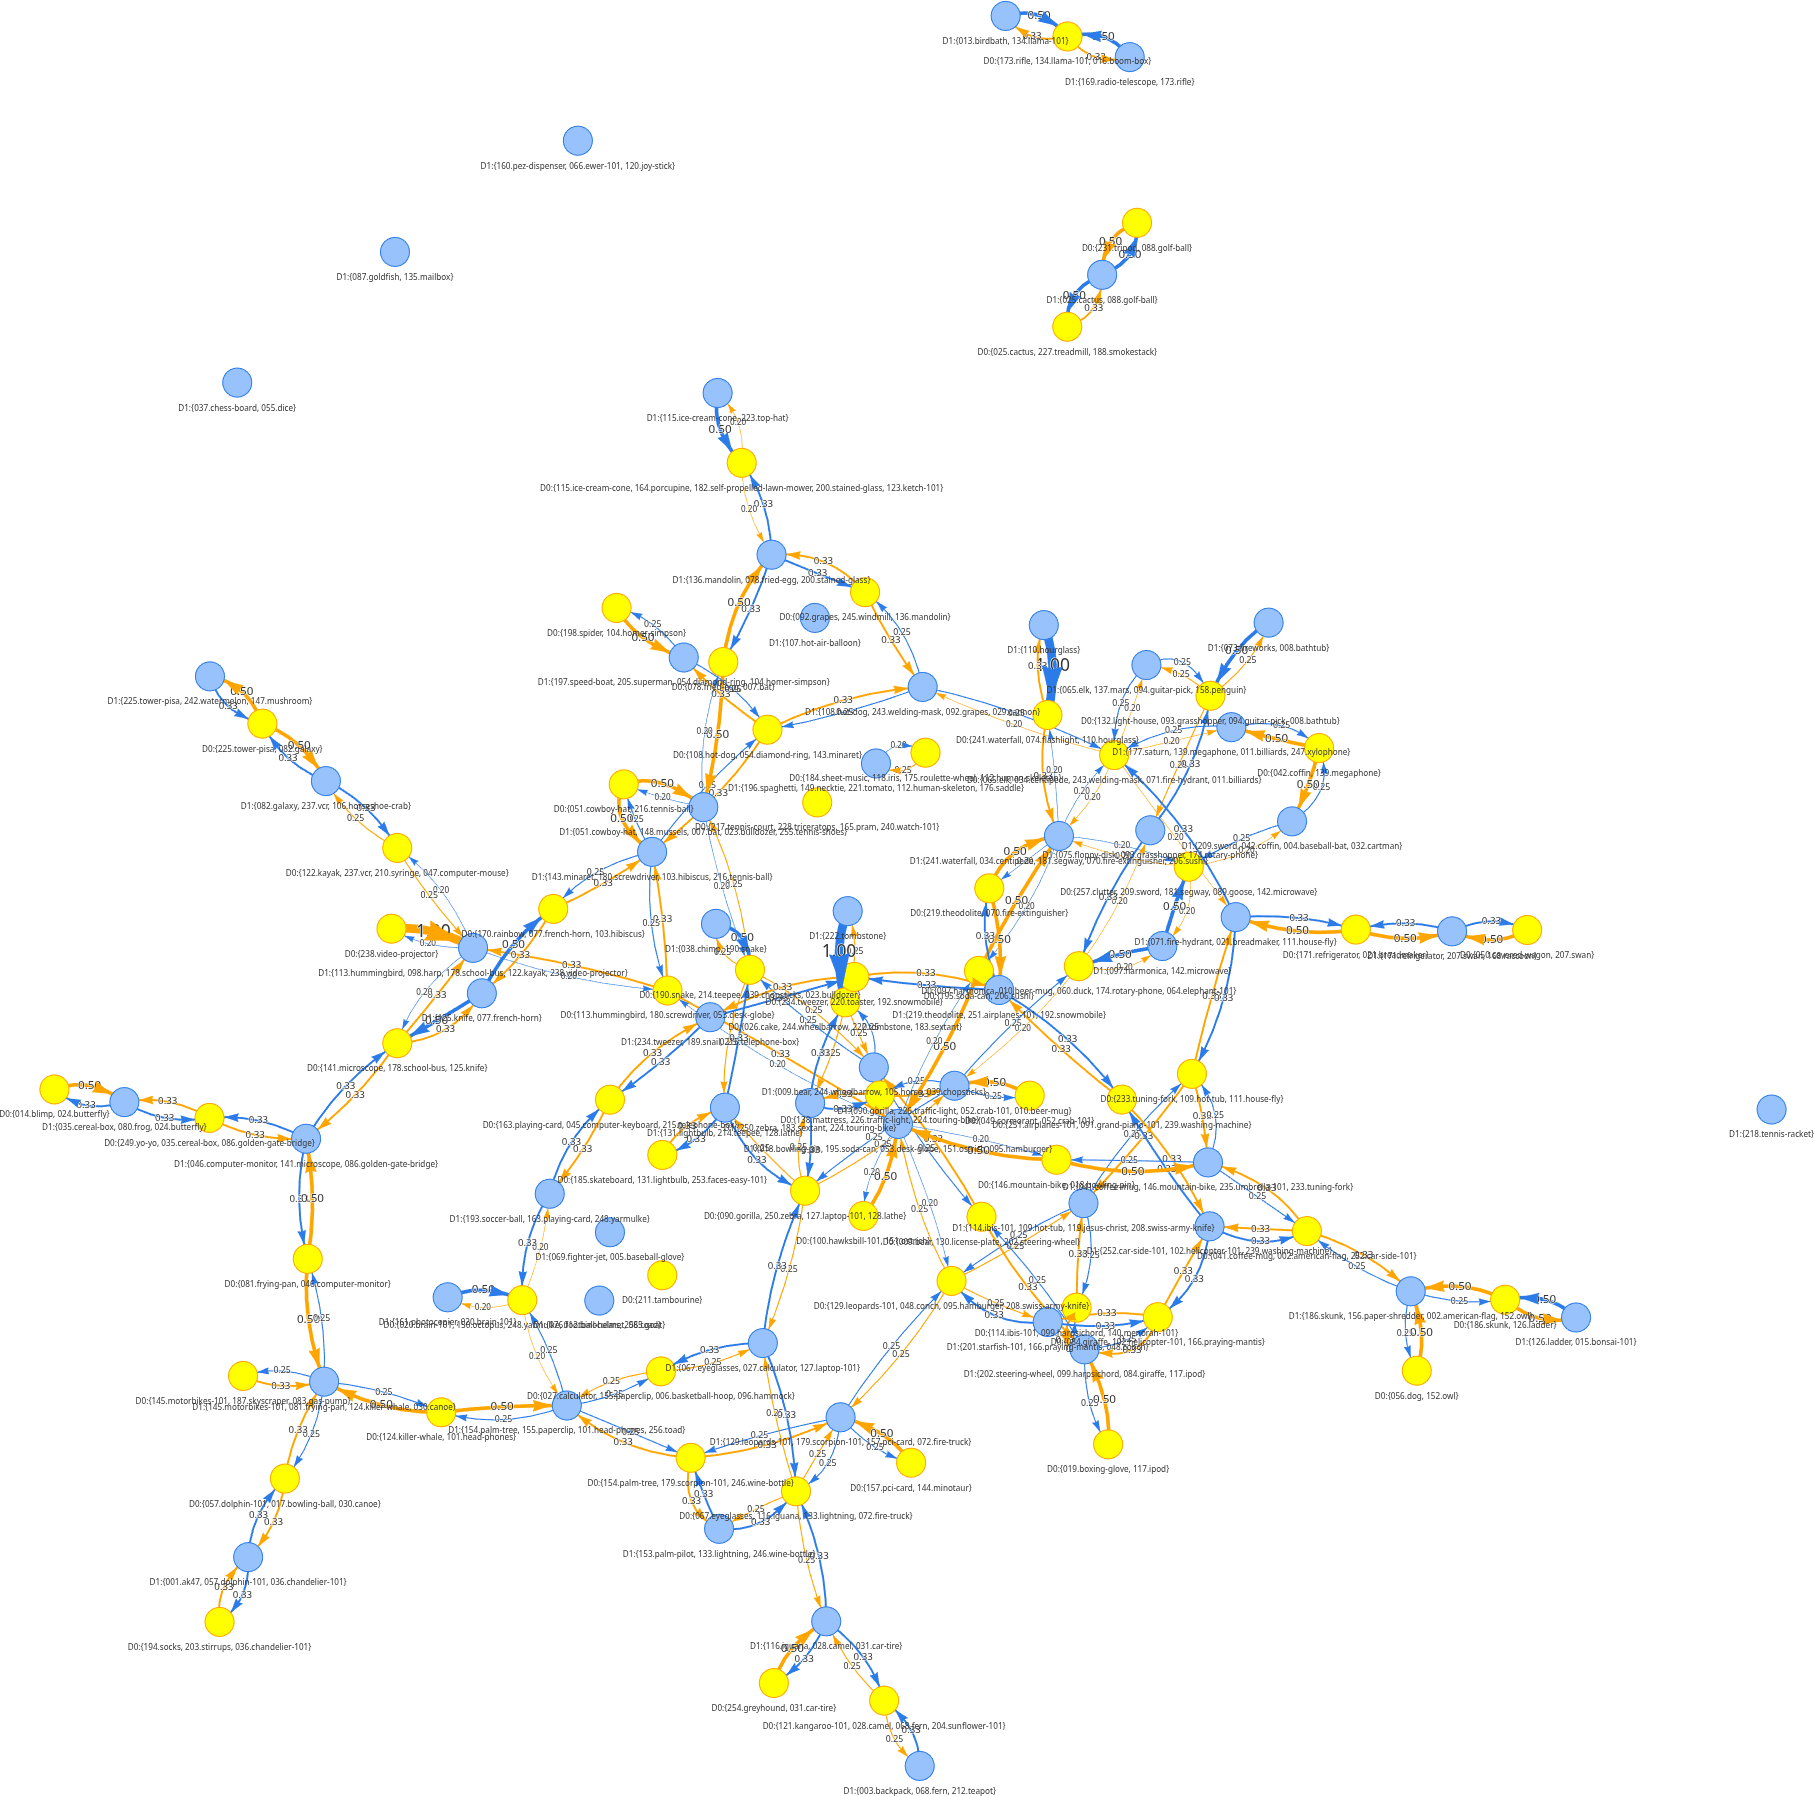
\includegraphics[width=\textwidth]{figures/caltech256_2domain.png}
            \caption{Caltech-256 2-domain variant 1\\
            ($\mu_{\text{concepts}}=180$, $\sigma^2_{\text{concepts}}=10$,\\
            $\mu_{\text{classes}}=3$, $\sigma^2_{\text{classes}}=1$)}
            \label{fig:caltech256_2domain}
      \end{subfigure}
      \hfill
      \begin{subfigure}[b]{0.4\textwidth}
            \centering
            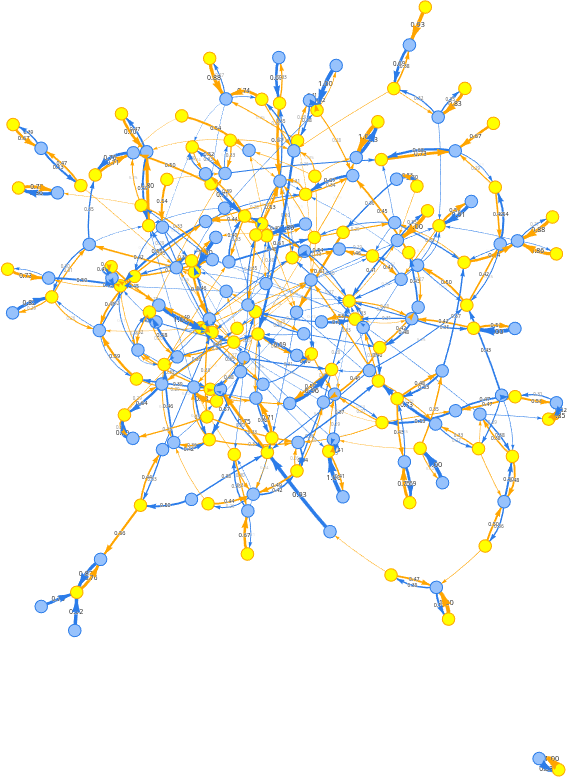
\includegraphics[width=\textwidth]{figures/caltech256_2domain_variant.png}
            \caption{Caltech-256 2-domain variant 2\\
            ($\mu_{\text{concepts}}=200$, $\sigma^2_{\text{concepts}}=10$,\\
            $\mu_{\text{classes}}=2$, $\sigma^2_{\text{classes}}=1$)}
            \label{fig:caltech256_2domain_variant}
      \end{subfigure}

      \begin{subfigure}[b]{0.4\textwidth}
            \centering
            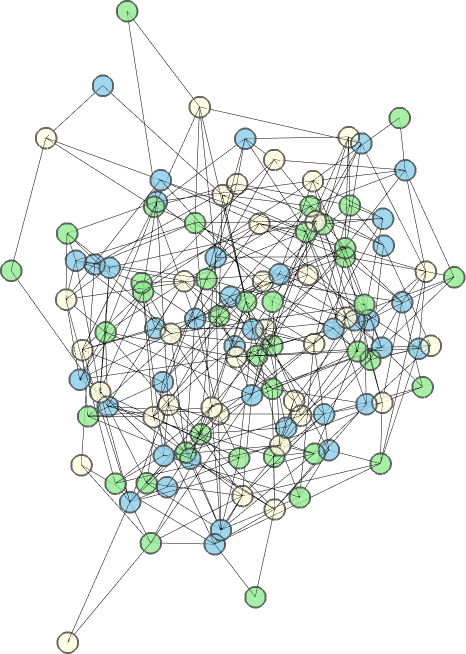
\includegraphics[width=\textwidth]{figures/caltech256_3domain.png}
            \caption{Caltech-256 3-domain variant\\
            ($\mu_{\text{concepts}}=180$, $\sigma^2_{\text{concepts}}=10$,\\
            $\mu_{\text{classes}}=5$, $\sigma^2_{\text{classes}}=1$)}
            \label{fig:caltech256_3domain}
      \end{subfigure}
      \hfill
      \begin{subfigure}[b]{0.4\textwidth}
            \centering
            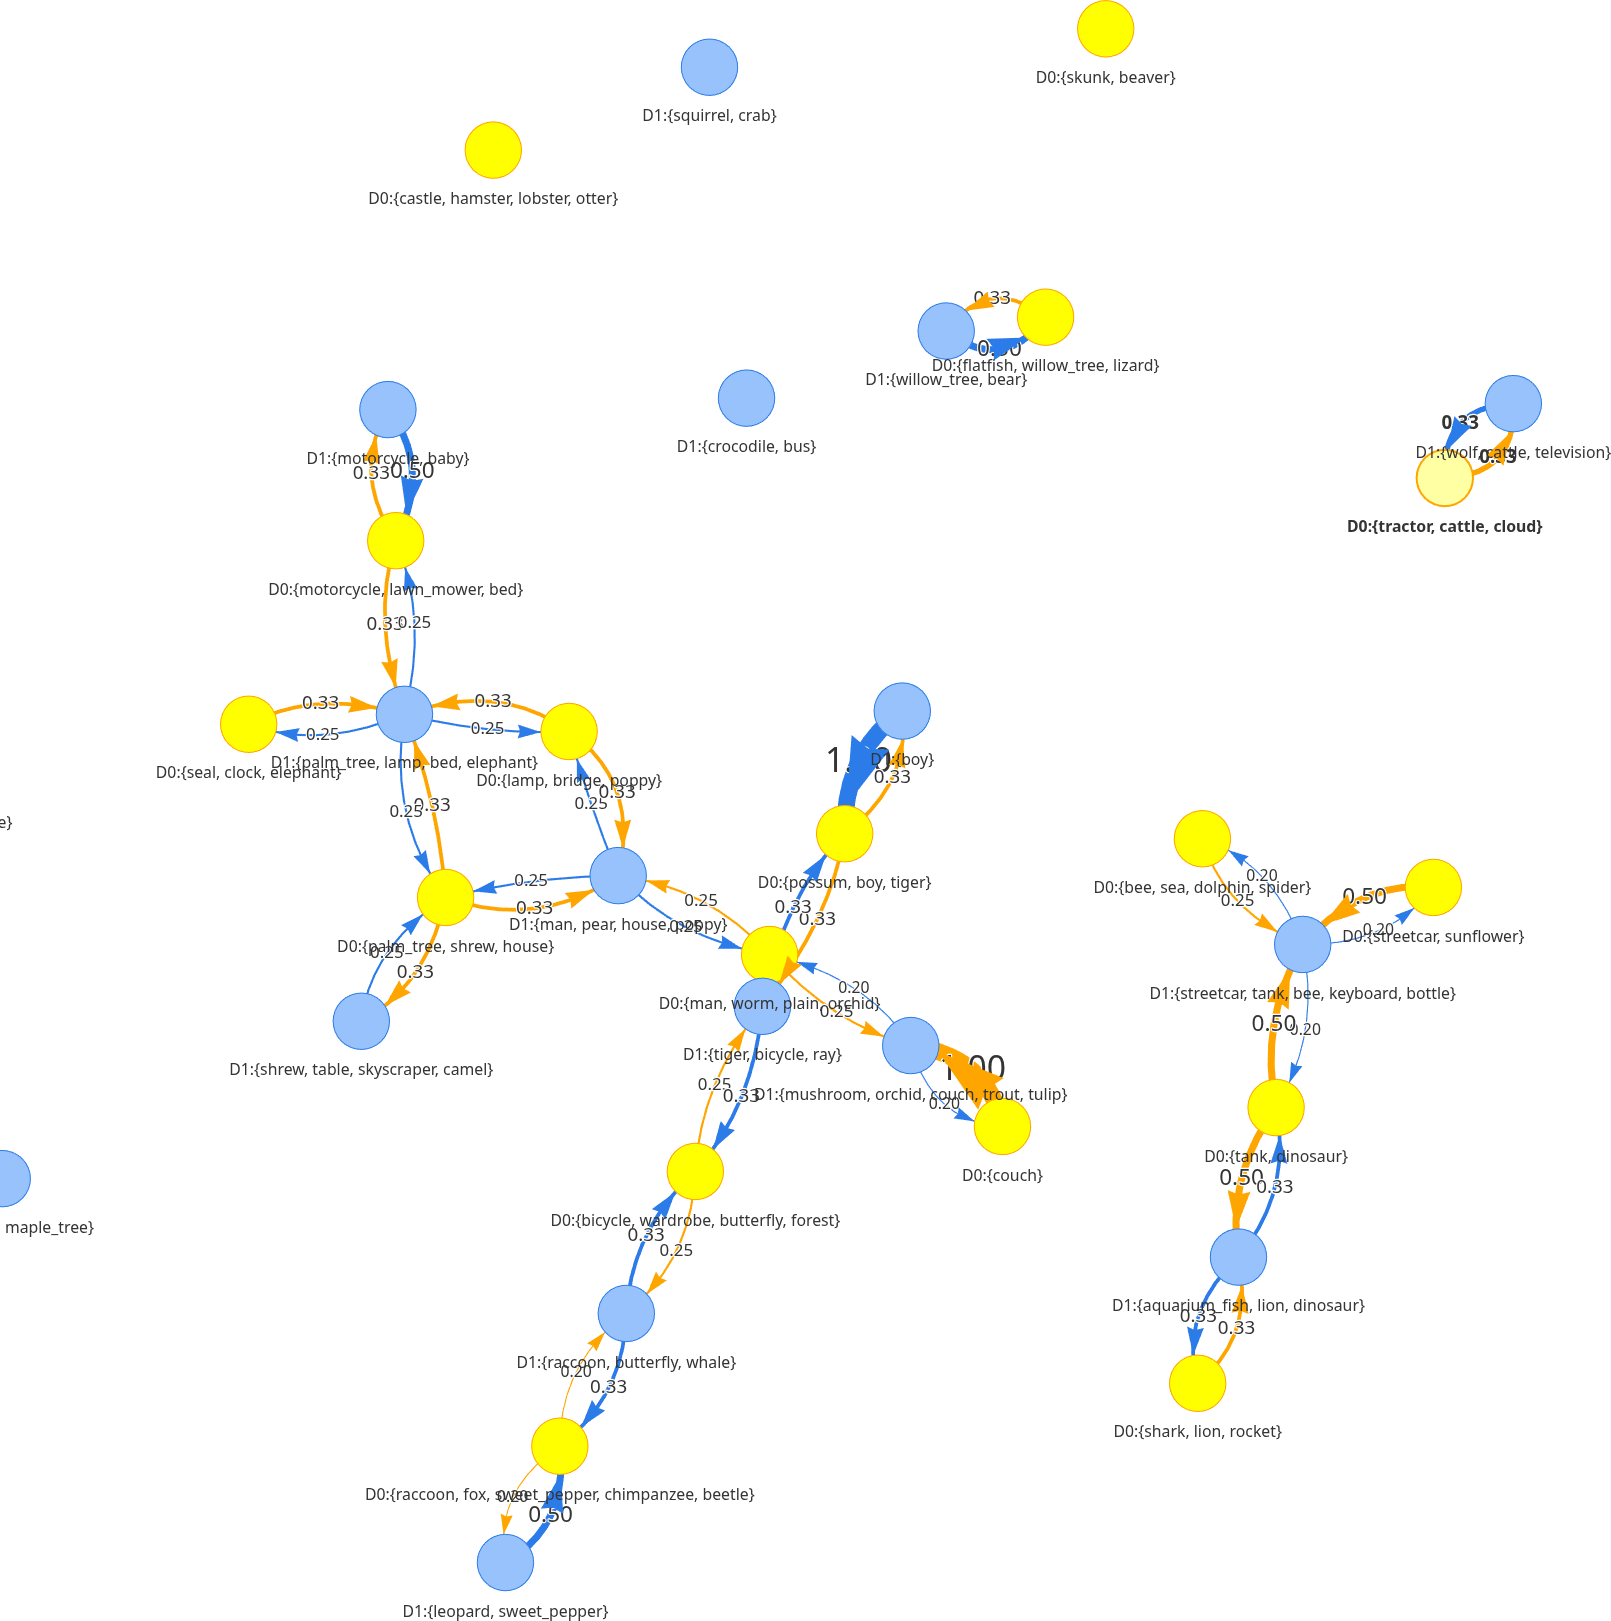
\includegraphics[width=\textwidth]{figures/cifar100_2domain.png}
            \caption{CIFAR-100 2-domain variant\\
            ($\mu_{\text{concepts}}=50$, $\sigma^2_{\text{concepts}}=5$,\\
            $\mu_{\text{classes}}=3$, $\sigma^2_{\text{classes}}=1$)}
            \label{fig:cifar100_2domain}
      \end{subfigure}

      \caption{Synthetic dataset variants showing their relationship graphs before applying universal taxonomy algorithms.
            The number of concepts and classes per concept are sampled from truncated normal distributions with the parameters shown in each subfigure caption.}
      \label{fig:synthetic_variants}
\end{figure}

\subsubsection{Model Accuracy}

Let us now take a look at the accuracy of our models trained on the synthetic dataset variants.
We use checkpoints to save the model after each epoch and pick the model checkpoint with the lowest validation loss
for our final evaluation.

We can see our final training runs in Figure~\ref{fig:all_training_runs}.
It can be observed that our overfitting mitigation techniques have worked sufficiently well,
as our training and validation accuracy curves do not diverge significantly.
We present the final model accuracies on the test sets in Table~\ref{tab:evaluation_results}.
Multiple things can be observed:
\begin{itemize}
      \item All the models achieve an accuracy of around 0.8 on the test set,
            which is an average performance for these datasets.
            Our focus is not on achieving state-of-the-art performance,
            but rather on creating models suitable for our cross-domain prediction task.
            It should be noted that a lower model accuracy will lead to worse performance
            in our relationship selection methods, but since we will compare the methods against each other
            using the same models, this should not be a problem.
      \item The CIFAR-100 variants have a slightly lower accuracy than the Caltech-256 variants,
            which is expected since the CIFAR-100 dataset has closely related classes
            categorised into superclasses, which make it harder for a model to distinguish between them.
      \item The number of concepts (i.e. classes) in the original dataset that get merged
            into a new class in the synthetic dataset variants does not seem to have a significant impact
            on the model accuracy: The Caltech-256 2-domain variant 2 has a $\mu_{\text{classes}}=2$,
            while the Caltech-256 3-domain variant has a $\mu_{\text{classes}}=5$,
            but the deviation in accuracy is negligible ($\leq 0.05$).
\end{itemize}

\begin{figure}[ht]
      \centering
      \scalebox{0.35}{%% Creator: Matplotlib, PGF backend
%%
%% To include the figure in your LaTeX document, write
%%   \input{<filename>.pgf}
%%
%% Make sure the required packages are loaded in your preamble
%%   \usepackage{pgf}
%%
%% Also ensure that all the required font packages are loaded; for instance,
%% the lmodern package is sometimes necessary when using math font.
%%   \usepackage{lmodern}
%%
%% Figures using additional raster images can only be included by \input if
%% they are in the same directory as the main LaTeX file. For loading figures
%% from other directories you can use the `import` package
%%   \usepackage{import}
%%
%% and then include the figures with
%%   \import{<path to file>}{<filename>.pgf}
%%
%% Matplotlib used the following preamble
%%   \def\mathdefault#1{#1}
%%   \everymath=\expandafter{\the\everymath\displaystyle}
%%   \IfFileExists{scrextend.sty}{
%%     \usepackage[fontsize=11.000000pt]{scrextend}
%%   }{
%%     \renewcommand{\normalsize}{\fontsize{11.000000}{13.200000}\selectfont}
%%     \normalsize
%%   }
%%   
%%   \ifdefined\pdftexversion\else  % non-pdftex case.
%%     \usepackage{fontspec}
%%     \setmainfont{DejaVuSerif.ttf}[Path=\detokenize{/home/sentinel/.conda/envs/master-thesis/lib/python3.13/site-packages/matplotlib/mpl-data/fonts/ttf/}]
%%     \setsansfont{DejaVuSans.ttf}[Path=\detokenize{/home/sentinel/.conda/envs/master-thesis/lib/python3.13/site-packages/matplotlib/mpl-data/fonts/ttf/}]
%%     \setmonofont{DejaVuSansMono.ttf}[Path=\detokenize{/home/sentinel/.conda/envs/master-thesis/lib/python3.13/site-packages/matplotlib/mpl-data/fonts/ttf/}]
%%   \fi
%%   \makeatletter\@ifpackageloaded{underscore}{}{\usepackage[strings]{underscore}}\makeatother
%%
\begingroup%
\makeatletter%
\begin{pgfpicture}%
\pgfpathrectangle{\pgfpointorigin}{\pgfqpoint{11.870000in}{9.870000in}}%
\pgfusepath{use as bounding box, clip}%
\begin{pgfscope}%
\pgfsetbuttcap%
\pgfsetmiterjoin%
\definecolor{currentfill}{rgb}{1.000000,1.000000,1.000000}%
\pgfsetfillcolor{currentfill}%
\pgfsetlinewidth{0.000000pt}%
\definecolor{currentstroke}{rgb}{1.000000,1.000000,1.000000}%
\pgfsetstrokecolor{currentstroke}%
\pgfsetdash{}{0pt}%
\pgfpathmoveto{\pgfqpoint{0.000000in}{0.000000in}}%
\pgfpathlineto{\pgfqpoint{11.870000in}{0.000000in}}%
\pgfpathlineto{\pgfqpoint{11.870000in}{9.870000in}}%
\pgfpathlineto{\pgfqpoint{0.000000in}{9.870000in}}%
\pgfpathlineto{\pgfqpoint{0.000000in}{0.000000in}}%
\pgfpathclose%
\pgfusepath{fill}%
\end{pgfscope}%
\begin{pgfscope}%
\pgfsetbuttcap%
\pgfsetmiterjoin%
\definecolor{currentfill}{rgb}{1.000000,1.000000,1.000000}%
\pgfsetfillcolor{currentfill}%
\pgfsetlinewidth{0.000000pt}%
\definecolor{currentstroke}{rgb}{0.000000,0.000000,0.000000}%
\pgfsetstrokecolor{currentstroke}%
\pgfsetstrokeopacity{0.000000}%
\pgfsetdash{}{0pt}%
\pgfpathmoveto{\pgfqpoint{0.594961in}{5.465986in}}%
\pgfpathlineto{\pgfqpoint{5.852500in}{5.465986in}}%
\pgfpathlineto{\pgfqpoint{5.852500in}{9.547376in}}%
\pgfpathlineto{\pgfqpoint{0.594961in}{9.547376in}}%
\pgfpathlineto{\pgfqpoint{0.594961in}{5.465986in}}%
\pgfpathclose%
\pgfusepath{fill}%
\end{pgfscope}%
\begin{pgfscope}%
\pgfpathrectangle{\pgfqpoint{0.594961in}{5.465986in}}{\pgfqpoint{5.257539in}{4.081390in}}%
\pgfusepath{clip}%
\pgfsetrectcap%
\pgfsetroundjoin%
\pgfsetlinewidth{0.803000pt}%
\definecolor{currentstroke}{rgb}{0.690196,0.690196,0.690196}%
\pgfsetstrokecolor{currentstroke}%
\pgfsetstrokeopacity{0.300000}%
\pgfsetdash{}{0pt}%
\pgfpathmoveto{\pgfqpoint{0.791125in}{5.465986in}}%
\pgfpathlineto{\pgfqpoint{0.791125in}{9.547376in}}%
\pgfusepath{stroke}%
\end{pgfscope}%
\begin{pgfscope}%
\pgfsetbuttcap%
\pgfsetroundjoin%
\definecolor{currentfill}{rgb}{0.000000,0.000000,0.000000}%
\pgfsetfillcolor{currentfill}%
\pgfsetlinewidth{0.803000pt}%
\definecolor{currentstroke}{rgb}{0.000000,0.000000,0.000000}%
\pgfsetstrokecolor{currentstroke}%
\pgfsetdash{}{0pt}%
\pgfsys@defobject{currentmarker}{\pgfqpoint{0.000000in}{-0.048611in}}{\pgfqpoint{0.000000in}{0.000000in}}{%
\pgfpathmoveto{\pgfqpoint{0.000000in}{0.000000in}}%
\pgfpathlineto{\pgfqpoint{0.000000in}{-0.048611in}}%
\pgfusepath{stroke,fill}%
}%
\begin{pgfscope}%
\pgfsys@transformshift{0.791125in}{5.465986in}%
\pgfsys@useobject{currentmarker}{}%
\end{pgfscope}%
\end{pgfscope}%
\begin{pgfscope}%
\definecolor{textcolor}{rgb}{0.000000,0.000000,0.000000}%
\pgfsetstrokecolor{textcolor}%
\pgfsetfillcolor{textcolor}%
\pgftext[x=0.791125in,y=5.368764in,,top]{\color{textcolor}{\fontsize{11.000000}{13.200000}\selectfont\catcode`\^=\active\def^{\ifmmode\sp\else\^{}\fi}\catcode`\%=\active\def%{\%}$\mathdefault{0}$}}%
\end{pgfscope}%
\begin{pgfscope}%
\pgfpathrectangle{\pgfqpoint{0.594961in}{5.465986in}}{\pgfqpoint{5.257539in}{4.081390in}}%
\pgfusepath{clip}%
\pgfsetrectcap%
\pgfsetroundjoin%
\pgfsetlinewidth{0.803000pt}%
\definecolor{currentstroke}{rgb}{0.690196,0.690196,0.690196}%
\pgfsetstrokecolor{currentstroke}%
\pgfsetstrokeopacity{0.300000}%
\pgfsetdash{}{0pt}%
\pgfpathmoveto{\pgfqpoint{1.664906in}{5.465986in}}%
\pgfpathlineto{\pgfqpoint{1.664906in}{9.547376in}}%
\pgfusepath{stroke}%
\end{pgfscope}%
\begin{pgfscope}%
\pgfsetbuttcap%
\pgfsetroundjoin%
\definecolor{currentfill}{rgb}{0.000000,0.000000,0.000000}%
\pgfsetfillcolor{currentfill}%
\pgfsetlinewidth{0.803000pt}%
\definecolor{currentstroke}{rgb}{0.000000,0.000000,0.000000}%
\pgfsetstrokecolor{currentstroke}%
\pgfsetdash{}{0pt}%
\pgfsys@defobject{currentmarker}{\pgfqpoint{0.000000in}{-0.048611in}}{\pgfqpoint{0.000000in}{0.000000in}}{%
\pgfpathmoveto{\pgfqpoint{0.000000in}{0.000000in}}%
\pgfpathlineto{\pgfqpoint{0.000000in}{-0.048611in}}%
\pgfusepath{stroke,fill}%
}%
\begin{pgfscope}%
\pgfsys@transformshift{1.664906in}{5.465986in}%
\pgfsys@useobject{currentmarker}{}%
\end{pgfscope}%
\end{pgfscope}%
\begin{pgfscope}%
\definecolor{textcolor}{rgb}{0.000000,0.000000,0.000000}%
\pgfsetstrokecolor{textcolor}%
\pgfsetfillcolor{textcolor}%
\pgftext[x=1.664906in,y=5.368764in,,top]{\color{textcolor}{\fontsize{11.000000}{13.200000}\selectfont\catcode`\^=\active\def^{\ifmmode\sp\else\^{}\fi}\catcode`\%=\active\def%{\%}$\mathdefault{1000}$}}%
\end{pgfscope}%
\begin{pgfscope}%
\pgfpathrectangle{\pgfqpoint{0.594961in}{5.465986in}}{\pgfqpoint{5.257539in}{4.081390in}}%
\pgfusepath{clip}%
\pgfsetrectcap%
\pgfsetroundjoin%
\pgfsetlinewidth{0.803000pt}%
\definecolor{currentstroke}{rgb}{0.690196,0.690196,0.690196}%
\pgfsetstrokecolor{currentstroke}%
\pgfsetstrokeopacity{0.300000}%
\pgfsetdash{}{0pt}%
\pgfpathmoveto{\pgfqpoint{2.538686in}{5.465986in}}%
\pgfpathlineto{\pgfqpoint{2.538686in}{9.547376in}}%
\pgfusepath{stroke}%
\end{pgfscope}%
\begin{pgfscope}%
\pgfsetbuttcap%
\pgfsetroundjoin%
\definecolor{currentfill}{rgb}{0.000000,0.000000,0.000000}%
\pgfsetfillcolor{currentfill}%
\pgfsetlinewidth{0.803000pt}%
\definecolor{currentstroke}{rgb}{0.000000,0.000000,0.000000}%
\pgfsetstrokecolor{currentstroke}%
\pgfsetdash{}{0pt}%
\pgfsys@defobject{currentmarker}{\pgfqpoint{0.000000in}{-0.048611in}}{\pgfqpoint{0.000000in}{0.000000in}}{%
\pgfpathmoveto{\pgfqpoint{0.000000in}{0.000000in}}%
\pgfpathlineto{\pgfqpoint{0.000000in}{-0.048611in}}%
\pgfusepath{stroke,fill}%
}%
\begin{pgfscope}%
\pgfsys@transformshift{2.538686in}{5.465986in}%
\pgfsys@useobject{currentmarker}{}%
\end{pgfscope}%
\end{pgfscope}%
\begin{pgfscope}%
\definecolor{textcolor}{rgb}{0.000000,0.000000,0.000000}%
\pgfsetstrokecolor{textcolor}%
\pgfsetfillcolor{textcolor}%
\pgftext[x=2.538686in,y=5.368764in,,top]{\color{textcolor}{\fontsize{11.000000}{13.200000}\selectfont\catcode`\^=\active\def^{\ifmmode\sp\else\^{}\fi}\catcode`\%=\active\def%{\%}$\mathdefault{2000}$}}%
\end{pgfscope}%
\begin{pgfscope}%
\pgfpathrectangle{\pgfqpoint{0.594961in}{5.465986in}}{\pgfqpoint{5.257539in}{4.081390in}}%
\pgfusepath{clip}%
\pgfsetrectcap%
\pgfsetroundjoin%
\pgfsetlinewidth{0.803000pt}%
\definecolor{currentstroke}{rgb}{0.690196,0.690196,0.690196}%
\pgfsetstrokecolor{currentstroke}%
\pgfsetstrokeopacity{0.300000}%
\pgfsetdash{}{0pt}%
\pgfpathmoveto{\pgfqpoint{3.412467in}{5.465986in}}%
\pgfpathlineto{\pgfqpoint{3.412467in}{9.547376in}}%
\pgfusepath{stroke}%
\end{pgfscope}%
\begin{pgfscope}%
\pgfsetbuttcap%
\pgfsetroundjoin%
\definecolor{currentfill}{rgb}{0.000000,0.000000,0.000000}%
\pgfsetfillcolor{currentfill}%
\pgfsetlinewidth{0.803000pt}%
\definecolor{currentstroke}{rgb}{0.000000,0.000000,0.000000}%
\pgfsetstrokecolor{currentstroke}%
\pgfsetdash{}{0pt}%
\pgfsys@defobject{currentmarker}{\pgfqpoint{0.000000in}{-0.048611in}}{\pgfqpoint{0.000000in}{0.000000in}}{%
\pgfpathmoveto{\pgfqpoint{0.000000in}{0.000000in}}%
\pgfpathlineto{\pgfqpoint{0.000000in}{-0.048611in}}%
\pgfusepath{stroke,fill}%
}%
\begin{pgfscope}%
\pgfsys@transformshift{3.412467in}{5.465986in}%
\pgfsys@useobject{currentmarker}{}%
\end{pgfscope}%
\end{pgfscope}%
\begin{pgfscope}%
\definecolor{textcolor}{rgb}{0.000000,0.000000,0.000000}%
\pgfsetstrokecolor{textcolor}%
\pgfsetfillcolor{textcolor}%
\pgftext[x=3.412467in,y=5.368764in,,top]{\color{textcolor}{\fontsize{11.000000}{13.200000}\selectfont\catcode`\^=\active\def^{\ifmmode\sp\else\^{}\fi}\catcode`\%=\active\def%{\%}$\mathdefault{3000}$}}%
\end{pgfscope}%
\begin{pgfscope}%
\pgfpathrectangle{\pgfqpoint{0.594961in}{5.465986in}}{\pgfqpoint{5.257539in}{4.081390in}}%
\pgfusepath{clip}%
\pgfsetrectcap%
\pgfsetroundjoin%
\pgfsetlinewidth{0.803000pt}%
\definecolor{currentstroke}{rgb}{0.690196,0.690196,0.690196}%
\pgfsetstrokecolor{currentstroke}%
\pgfsetstrokeopacity{0.300000}%
\pgfsetdash{}{0pt}%
\pgfpathmoveto{\pgfqpoint{4.286248in}{5.465986in}}%
\pgfpathlineto{\pgfqpoint{4.286248in}{9.547376in}}%
\pgfusepath{stroke}%
\end{pgfscope}%
\begin{pgfscope}%
\pgfsetbuttcap%
\pgfsetroundjoin%
\definecolor{currentfill}{rgb}{0.000000,0.000000,0.000000}%
\pgfsetfillcolor{currentfill}%
\pgfsetlinewidth{0.803000pt}%
\definecolor{currentstroke}{rgb}{0.000000,0.000000,0.000000}%
\pgfsetstrokecolor{currentstroke}%
\pgfsetdash{}{0pt}%
\pgfsys@defobject{currentmarker}{\pgfqpoint{0.000000in}{-0.048611in}}{\pgfqpoint{0.000000in}{0.000000in}}{%
\pgfpathmoveto{\pgfqpoint{0.000000in}{0.000000in}}%
\pgfpathlineto{\pgfqpoint{0.000000in}{-0.048611in}}%
\pgfusepath{stroke,fill}%
}%
\begin{pgfscope}%
\pgfsys@transformshift{4.286248in}{5.465986in}%
\pgfsys@useobject{currentmarker}{}%
\end{pgfscope}%
\end{pgfscope}%
\begin{pgfscope}%
\definecolor{textcolor}{rgb}{0.000000,0.000000,0.000000}%
\pgfsetstrokecolor{textcolor}%
\pgfsetfillcolor{textcolor}%
\pgftext[x=4.286248in,y=5.368764in,,top]{\color{textcolor}{\fontsize{11.000000}{13.200000}\selectfont\catcode`\^=\active\def^{\ifmmode\sp\else\^{}\fi}\catcode`\%=\active\def%{\%}$\mathdefault{4000}$}}%
\end{pgfscope}%
\begin{pgfscope}%
\pgfpathrectangle{\pgfqpoint{0.594961in}{5.465986in}}{\pgfqpoint{5.257539in}{4.081390in}}%
\pgfusepath{clip}%
\pgfsetrectcap%
\pgfsetroundjoin%
\pgfsetlinewidth{0.803000pt}%
\definecolor{currentstroke}{rgb}{0.690196,0.690196,0.690196}%
\pgfsetstrokecolor{currentstroke}%
\pgfsetstrokeopacity{0.300000}%
\pgfsetdash{}{0pt}%
\pgfpathmoveto{\pgfqpoint{5.160029in}{5.465986in}}%
\pgfpathlineto{\pgfqpoint{5.160029in}{9.547376in}}%
\pgfusepath{stroke}%
\end{pgfscope}%
\begin{pgfscope}%
\pgfsetbuttcap%
\pgfsetroundjoin%
\definecolor{currentfill}{rgb}{0.000000,0.000000,0.000000}%
\pgfsetfillcolor{currentfill}%
\pgfsetlinewidth{0.803000pt}%
\definecolor{currentstroke}{rgb}{0.000000,0.000000,0.000000}%
\pgfsetstrokecolor{currentstroke}%
\pgfsetdash{}{0pt}%
\pgfsys@defobject{currentmarker}{\pgfqpoint{0.000000in}{-0.048611in}}{\pgfqpoint{0.000000in}{0.000000in}}{%
\pgfpathmoveto{\pgfqpoint{0.000000in}{0.000000in}}%
\pgfpathlineto{\pgfqpoint{0.000000in}{-0.048611in}}%
\pgfusepath{stroke,fill}%
}%
\begin{pgfscope}%
\pgfsys@transformshift{5.160029in}{5.465986in}%
\pgfsys@useobject{currentmarker}{}%
\end{pgfscope}%
\end{pgfscope}%
\begin{pgfscope}%
\definecolor{textcolor}{rgb}{0.000000,0.000000,0.000000}%
\pgfsetstrokecolor{textcolor}%
\pgfsetfillcolor{textcolor}%
\pgftext[x=5.160029in,y=5.368764in,,top]{\color{textcolor}{\fontsize{11.000000}{13.200000}\selectfont\catcode`\^=\active\def^{\ifmmode\sp\else\^{}\fi}\catcode`\%=\active\def%{\%}$\mathdefault{5000}$}}%
\end{pgfscope}%
\begin{pgfscope}%
\definecolor{textcolor}{rgb}{0.000000,0.000000,0.000000}%
\pgfsetstrokecolor{textcolor}%
\pgfsetfillcolor{textcolor}%
\pgftext[x=3.223730in,y=5.165354in,,top]{\color{textcolor}{\fontsize{11.000000}{13.200000}\selectfont\catcode`\^=\active\def^{\ifmmode\sp\else\^{}\fi}\catcode`\%=\active\def%{\%}Steps}}%
\end{pgfscope}%
\begin{pgfscope}%
\pgfpathrectangle{\pgfqpoint{0.594961in}{5.465986in}}{\pgfqpoint{5.257539in}{4.081390in}}%
\pgfusepath{clip}%
\pgfsetrectcap%
\pgfsetroundjoin%
\pgfsetlinewidth{0.803000pt}%
\definecolor{currentstroke}{rgb}{0.690196,0.690196,0.690196}%
\pgfsetstrokecolor{currentstroke}%
\pgfsetstrokeopacity{0.300000}%
\pgfsetdash{}{0pt}%
\pgfpathmoveto{\pgfqpoint{0.594961in}{5.907856in}}%
\pgfpathlineto{\pgfqpoint{5.852500in}{5.907856in}}%
\pgfusepath{stroke}%
\end{pgfscope}%
\begin{pgfscope}%
\pgfsetbuttcap%
\pgfsetroundjoin%
\definecolor{currentfill}{rgb}{0.000000,0.000000,0.000000}%
\pgfsetfillcolor{currentfill}%
\pgfsetlinewidth{0.803000pt}%
\definecolor{currentstroke}{rgb}{0.000000,0.000000,0.000000}%
\pgfsetstrokecolor{currentstroke}%
\pgfsetdash{}{0pt}%
\pgfsys@defobject{currentmarker}{\pgfqpoint{-0.048611in}{0.000000in}}{\pgfqpoint{-0.000000in}{0.000000in}}{%
\pgfpathmoveto{\pgfqpoint{-0.000000in}{0.000000in}}%
\pgfpathlineto{\pgfqpoint{-0.048611in}{0.000000in}}%
\pgfusepath{stroke,fill}%
}%
\begin{pgfscope}%
\pgfsys@transformshift{0.594961in}{5.907856in}%
\pgfsys@useobject{currentmarker}{}%
\end{pgfscope}%
\end{pgfscope}%
\begin{pgfscope}%
\definecolor{textcolor}{rgb}{0.000000,0.000000,0.000000}%
\pgfsetstrokecolor{textcolor}%
\pgfsetfillcolor{textcolor}%
\pgftext[x=0.303410in, y=5.849818in, left, base]{\color{textcolor}{\fontsize{11.000000}{13.200000}\selectfont\catcode`\^=\active\def^{\ifmmode\sp\else\^{}\fi}\catcode`\%=\active\def%{\%}$\mathdefault{0.2}$}}%
\end{pgfscope}%
\begin{pgfscope}%
\pgfpathrectangle{\pgfqpoint{0.594961in}{5.465986in}}{\pgfqpoint{5.257539in}{4.081390in}}%
\pgfusepath{clip}%
\pgfsetrectcap%
\pgfsetroundjoin%
\pgfsetlinewidth{0.803000pt}%
\definecolor{currentstroke}{rgb}{0.690196,0.690196,0.690196}%
\pgfsetstrokecolor{currentstroke}%
\pgfsetstrokeopacity{0.300000}%
\pgfsetdash{}{0pt}%
\pgfpathmoveto{\pgfqpoint{0.594961in}{6.771357in}}%
\pgfpathlineto{\pgfqpoint{5.852500in}{6.771357in}}%
\pgfusepath{stroke}%
\end{pgfscope}%
\begin{pgfscope}%
\pgfsetbuttcap%
\pgfsetroundjoin%
\definecolor{currentfill}{rgb}{0.000000,0.000000,0.000000}%
\pgfsetfillcolor{currentfill}%
\pgfsetlinewidth{0.803000pt}%
\definecolor{currentstroke}{rgb}{0.000000,0.000000,0.000000}%
\pgfsetstrokecolor{currentstroke}%
\pgfsetdash{}{0pt}%
\pgfsys@defobject{currentmarker}{\pgfqpoint{-0.048611in}{0.000000in}}{\pgfqpoint{-0.000000in}{0.000000in}}{%
\pgfpathmoveto{\pgfqpoint{-0.000000in}{0.000000in}}%
\pgfpathlineto{\pgfqpoint{-0.048611in}{0.000000in}}%
\pgfusepath{stroke,fill}%
}%
\begin{pgfscope}%
\pgfsys@transformshift{0.594961in}{6.771357in}%
\pgfsys@useobject{currentmarker}{}%
\end{pgfscope}%
\end{pgfscope}%
\begin{pgfscope}%
\definecolor{textcolor}{rgb}{0.000000,0.000000,0.000000}%
\pgfsetstrokecolor{textcolor}%
\pgfsetfillcolor{textcolor}%
\pgftext[x=0.303410in, y=6.713319in, left, base]{\color{textcolor}{\fontsize{11.000000}{13.200000}\selectfont\catcode`\^=\active\def^{\ifmmode\sp\else\^{}\fi}\catcode`\%=\active\def%{\%}$\mathdefault{0.4}$}}%
\end{pgfscope}%
\begin{pgfscope}%
\pgfpathrectangle{\pgfqpoint{0.594961in}{5.465986in}}{\pgfqpoint{5.257539in}{4.081390in}}%
\pgfusepath{clip}%
\pgfsetrectcap%
\pgfsetroundjoin%
\pgfsetlinewidth{0.803000pt}%
\definecolor{currentstroke}{rgb}{0.690196,0.690196,0.690196}%
\pgfsetstrokecolor{currentstroke}%
\pgfsetstrokeopacity{0.300000}%
\pgfsetdash{}{0pt}%
\pgfpathmoveto{\pgfqpoint{0.594961in}{7.634857in}}%
\pgfpathlineto{\pgfqpoint{5.852500in}{7.634857in}}%
\pgfusepath{stroke}%
\end{pgfscope}%
\begin{pgfscope}%
\pgfsetbuttcap%
\pgfsetroundjoin%
\definecolor{currentfill}{rgb}{0.000000,0.000000,0.000000}%
\pgfsetfillcolor{currentfill}%
\pgfsetlinewidth{0.803000pt}%
\definecolor{currentstroke}{rgb}{0.000000,0.000000,0.000000}%
\pgfsetstrokecolor{currentstroke}%
\pgfsetdash{}{0pt}%
\pgfsys@defobject{currentmarker}{\pgfqpoint{-0.048611in}{0.000000in}}{\pgfqpoint{-0.000000in}{0.000000in}}{%
\pgfpathmoveto{\pgfqpoint{-0.000000in}{0.000000in}}%
\pgfpathlineto{\pgfqpoint{-0.048611in}{0.000000in}}%
\pgfusepath{stroke,fill}%
}%
\begin{pgfscope}%
\pgfsys@transformshift{0.594961in}{7.634857in}%
\pgfsys@useobject{currentmarker}{}%
\end{pgfscope}%
\end{pgfscope}%
\begin{pgfscope}%
\definecolor{textcolor}{rgb}{0.000000,0.000000,0.000000}%
\pgfsetstrokecolor{textcolor}%
\pgfsetfillcolor{textcolor}%
\pgftext[x=0.303410in, y=7.576820in, left, base]{\color{textcolor}{\fontsize{11.000000}{13.200000}\selectfont\catcode`\^=\active\def^{\ifmmode\sp\else\^{}\fi}\catcode`\%=\active\def%{\%}$\mathdefault{0.6}$}}%
\end{pgfscope}%
\begin{pgfscope}%
\pgfpathrectangle{\pgfqpoint{0.594961in}{5.465986in}}{\pgfqpoint{5.257539in}{4.081390in}}%
\pgfusepath{clip}%
\pgfsetrectcap%
\pgfsetroundjoin%
\pgfsetlinewidth{0.803000pt}%
\definecolor{currentstroke}{rgb}{0.690196,0.690196,0.690196}%
\pgfsetstrokecolor{currentstroke}%
\pgfsetstrokeopacity{0.300000}%
\pgfsetdash{}{0pt}%
\pgfpathmoveto{\pgfqpoint{0.594961in}{8.498358in}}%
\pgfpathlineto{\pgfqpoint{5.852500in}{8.498358in}}%
\pgfusepath{stroke}%
\end{pgfscope}%
\begin{pgfscope}%
\pgfsetbuttcap%
\pgfsetroundjoin%
\definecolor{currentfill}{rgb}{0.000000,0.000000,0.000000}%
\pgfsetfillcolor{currentfill}%
\pgfsetlinewidth{0.803000pt}%
\definecolor{currentstroke}{rgb}{0.000000,0.000000,0.000000}%
\pgfsetstrokecolor{currentstroke}%
\pgfsetdash{}{0pt}%
\pgfsys@defobject{currentmarker}{\pgfqpoint{-0.048611in}{0.000000in}}{\pgfqpoint{-0.000000in}{0.000000in}}{%
\pgfpathmoveto{\pgfqpoint{-0.000000in}{0.000000in}}%
\pgfpathlineto{\pgfqpoint{-0.048611in}{0.000000in}}%
\pgfusepath{stroke,fill}%
}%
\begin{pgfscope}%
\pgfsys@transformshift{0.594961in}{8.498358in}%
\pgfsys@useobject{currentmarker}{}%
\end{pgfscope}%
\end{pgfscope}%
\begin{pgfscope}%
\definecolor{textcolor}{rgb}{0.000000,0.000000,0.000000}%
\pgfsetstrokecolor{textcolor}%
\pgfsetfillcolor{textcolor}%
\pgftext[x=0.303410in, y=8.440320in, left, base]{\color{textcolor}{\fontsize{11.000000}{13.200000}\selectfont\catcode`\^=\active\def^{\ifmmode\sp\else\^{}\fi}\catcode`\%=\active\def%{\%}$\mathdefault{0.8}$}}%
\end{pgfscope}%
\begin{pgfscope}%
\pgfpathrectangle{\pgfqpoint{0.594961in}{5.465986in}}{\pgfqpoint{5.257539in}{4.081390in}}%
\pgfusepath{clip}%
\pgfsetrectcap%
\pgfsetroundjoin%
\pgfsetlinewidth{0.803000pt}%
\definecolor{currentstroke}{rgb}{0.690196,0.690196,0.690196}%
\pgfsetstrokecolor{currentstroke}%
\pgfsetstrokeopacity{0.300000}%
\pgfsetdash{}{0pt}%
\pgfpathmoveto{\pgfqpoint{0.594961in}{9.361859in}}%
\pgfpathlineto{\pgfqpoint{5.852500in}{9.361859in}}%
\pgfusepath{stroke}%
\end{pgfscope}%
\begin{pgfscope}%
\pgfsetbuttcap%
\pgfsetroundjoin%
\definecolor{currentfill}{rgb}{0.000000,0.000000,0.000000}%
\pgfsetfillcolor{currentfill}%
\pgfsetlinewidth{0.803000pt}%
\definecolor{currentstroke}{rgb}{0.000000,0.000000,0.000000}%
\pgfsetstrokecolor{currentstroke}%
\pgfsetdash{}{0pt}%
\pgfsys@defobject{currentmarker}{\pgfqpoint{-0.048611in}{0.000000in}}{\pgfqpoint{-0.000000in}{0.000000in}}{%
\pgfpathmoveto{\pgfqpoint{-0.000000in}{0.000000in}}%
\pgfpathlineto{\pgfqpoint{-0.048611in}{0.000000in}}%
\pgfusepath{stroke,fill}%
}%
\begin{pgfscope}%
\pgfsys@transformshift{0.594961in}{9.361859in}%
\pgfsys@useobject{currentmarker}{}%
\end{pgfscope}%
\end{pgfscope}%
\begin{pgfscope}%
\definecolor{textcolor}{rgb}{0.000000,0.000000,0.000000}%
\pgfsetstrokecolor{textcolor}%
\pgfsetfillcolor{textcolor}%
\pgftext[x=0.303410in, y=9.303821in, left, base]{\color{textcolor}{\fontsize{11.000000}{13.200000}\selectfont\catcode`\^=\active\def^{\ifmmode\sp\else\^{}\fi}\catcode`\%=\active\def%{\%}$\mathdefault{1.0}$}}%
\end{pgfscope}%
\begin{pgfscope}%
\definecolor{textcolor}{rgb}{0.000000,0.000000,0.000000}%
\pgfsetstrokecolor{textcolor}%
\pgfsetfillcolor{textcolor}%
\pgftext[x=0.247854in,y=7.506681in,,bottom,rotate=90.000000]{\color{textcolor}{\fontsize{11.000000}{13.200000}\selectfont\catcode`\^=\active\def^{\ifmmode\sp\else\^{}\fi}\catcode`\%=\active\def%{\%}Accuracy}}%
\end{pgfscope}%
\begin{pgfscope}%
\pgfpathrectangle{\pgfqpoint{0.594961in}{5.465986in}}{\pgfqpoint{5.257539in}{4.081390in}}%
\pgfusepath{clip}%
\pgfsetrectcap%
\pgfsetroundjoin%
\pgfsetlinewidth{1.505625pt}%
\definecolor{currentstroke}{rgb}{0.121569,0.466667,0.705882}%
\pgfsetstrokecolor{currentstroke}%
\pgfsetdash{}{0pt}%
\pgfpathmoveto{\pgfqpoint{0.833940in}{5.651504in}}%
\pgfpathlineto{\pgfqpoint{0.877629in}{5.718965in}}%
\pgfpathlineto{\pgfqpoint{0.921318in}{5.921348in}}%
\pgfpathlineto{\pgfqpoint{0.965007in}{6.798341in}}%
\pgfpathlineto{\pgfqpoint{1.008696in}{7.135646in}}%
\pgfpathlineto{\pgfqpoint{1.052385in}{7.270568in}}%
\pgfpathlineto{\pgfqpoint{1.096074in}{7.877717in}}%
\pgfpathlineto{\pgfqpoint{1.139763in}{7.877717in}}%
\pgfpathlineto{\pgfqpoint{1.183452in}{8.215022in}}%
\pgfpathlineto{\pgfqpoint{1.227141in}{8.417405in}}%
\pgfpathlineto{\pgfqpoint{1.270830in}{8.687249in}}%
\pgfpathlineto{\pgfqpoint{1.314519in}{8.484866in}}%
\pgfpathlineto{\pgfqpoint{1.358208in}{8.619788in}}%
\pgfpathlineto{\pgfqpoint{1.401898in}{8.147561in}}%
\pgfpathlineto{\pgfqpoint{1.445587in}{8.957093in}}%
\pgfpathlineto{\pgfqpoint{1.489276in}{8.619788in}}%
\pgfpathlineto{\pgfqpoint{1.532965in}{8.889632in}}%
\pgfpathlineto{\pgfqpoint{1.576654in}{8.754710in}}%
\pgfpathlineto{\pgfqpoint{1.620343in}{9.024554in}}%
\pgfpathlineto{\pgfqpoint{1.664032in}{9.024554in}}%
\pgfpathlineto{\pgfqpoint{1.707721in}{8.417405in}}%
\pgfpathlineto{\pgfqpoint{1.751410in}{8.552327in}}%
\pgfpathlineto{\pgfqpoint{1.795099in}{8.619788in}}%
\pgfpathlineto{\pgfqpoint{1.838788in}{8.754710in}}%
\pgfpathlineto{\pgfqpoint{1.882477in}{8.687249in}}%
\pgfpathlineto{\pgfqpoint{1.926166in}{8.822171in}}%
\pgfpathlineto{\pgfqpoint{1.969855in}{9.226937in}}%
\pgfpathlineto{\pgfqpoint{2.013544in}{9.092015in}}%
\pgfpathlineto{\pgfqpoint{2.057233in}{8.889632in}}%
\pgfpathlineto{\pgfqpoint{2.100922in}{8.957093in}}%
\pgfpathlineto{\pgfqpoint{2.144611in}{8.889632in}}%
\pgfpathlineto{\pgfqpoint{2.188300in}{9.024554in}}%
\pgfpathlineto{\pgfqpoint{2.231989in}{8.957093in}}%
\pgfpathlineto{\pgfqpoint{2.275678in}{9.159476in}}%
\pgfpathlineto{\pgfqpoint{2.319367in}{9.092015in}}%
\pgfpathlineto{\pgfqpoint{2.363056in}{9.092015in}}%
\pgfpathlineto{\pgfqpoint{2.406745in}{9.024554in}}%
\pgfpathlineto{\pgfqpoint{2.450434in}{9.159476in}}%
\pgfpathlineto{\pgfqpoint{2.494124in}{9.226937in}}%
\pgfpathlineto{\pgfqpoint{2.537813in}{9.092015in}}%
\pgfpathlineto{\pgfqpoint{2.581502in}{9.092015in}}%
\pgfpathlineto{\pgfqpoint{2.625191in}{8.889632in}}%
\pgfpathlineto{\pgfqpoint{2.668880in}{9.159476in}}%
\pgfpathlineto{\pgfqpoint{2.712569in}{8.889632in}}%
\pgfpathlineto{\pgfqpoint{2.756258in}{9.159476in}}%
\pgfpathlineto{\pgfqpoint{2.799947in}{8.687249in}}%
\pgfpathlineto{\pgfqpoint{2.843636in}{9.024554in}}%
\pgfpathlineto{\pgfqpoint{2.887325in}{9.024554in}}%
\pgfpathlineto{\pgfqpoint{2.931014in}{9.159476in}}%
\pgfpathlineto{\pgfqpoint{2.974703in}{9.226937in}}%
\pgfpathlineto{\pgfqpoint{3.018392in}{9.092015in}}%
\pgfpathlineto{\pgfqpoint{3.062081in}{9.024554in}}%
\pgfpathlineto{\pgfqpoint{3.105770in}{9.024554in}}%
\pgfpathlineto{\pgfqpoint{3.149459in}{9.294398in}}%
\pgfpathlineto{\pgfqpoint{3.193148in}{9.024554in}}%
\pgfpathlineto{\pgfqpoint{3.236837in}{9.226937in}}%
\pgfpathlineto{\pgfqpoint{3.280526in}{9.159476in}}%
\pgfpathlineto{\pgfqpoint{3.324215in}{9.092015in}}%
\pgfpathlineto{\pgfqpoint{3.367904in}{9.361859in}}%
\pgfpathlineto{\pgfqpoint{3.411593in}{9.294398in}}%
\pgfpathlineto{\pgfqpoint{3.455282in}{9.226937in}}%
\pgfpathlineto{\pgfqpoint{3.498971in}{9.294398in}}%
\pgfpathlineto{\pgfqpoint{3.542660in}{9.159476in}}%
\pgfpathlineto{\pgfqpoint{3.586350in}{9.024554in}}%
\pgfpathlineto{\pgfqpoint{3.630039in}{9.092015in}}%
\pgfpathlineto{\pgfqpoint{3.673728in}{9.159476in}}%
\pgfpathlineto{\pgfqpoint{3.717417in}{8.957093in}}%
\pgfpathlineto{\pgfqpoint{3.761106in}{9.159476in}}%
\pgfpathlineto{\pgfqpoint{3.804795in}{9.226937in}}%
\pgfpathlineto{\pgfqpoint{3.848484in}{9.226937in}}%
\pgfpathlineto{\pgfqpoint{3.892173in}{9.226937in}}%
\pgfpathlineto{\pgfqpoint{3.935862in}{9.226937in}}%
\pgfpathlineto{\pgfqpoint{3.979551in}{9.361859in}}%
\pgfpathlineto{\pgfqpoint{4.023240in}{9.226937in}}%
\pgfpathlineto{\pgfqpoint{4.066929in}{9.361859in}}%
\pgfpathlineto{\pgfqpoint{4.110618in}{9.159476in}}%
\pgfpathlineto{\pgfqpoint{4.154307in}{9.294398in}}%
\pgfpathlineto{\pgfqpoint{4.197996in}{9.294398in}}%
\pgfpathlineto{\pgfqpoint{4.241685in}{9.092015in}}%
\pgfpathlineto{\pgfqpoint{4.285374in}{9.159476in}}%
\pgfpathlineto{\pgfqpoint{4.329063in}{9.294398in}}%
\pgfpathlineto{\pgfqpoint{4.372752in}{9.294398in}}%
\pgfpathlineto{\pgfqpoint{4.416441in}{9.226937in}}%
\pgfpathlineto{\pgfqpoint{4.460130in}{9.024554in}}%
\pgfpathlineto{\pgfqpoint{4.503819in}{9.226937in}}%
\pgfpathlineto{\pgfqpoint{4.547508in}{9.226937in}}%
\pgfpathlineto{\pgfqpoint{4.591197in}{9.092015in}}%
\pgfpathlineto{\pgfqpoint{4.634886in}{9.226937in}}%
\pgfpathlineto{\pgfqpoint{4.678576in}{9.361859in}}%
\pgfpathlineto{\pgfqpoint{4.722265in}{9.294398in}}%
\pgfpathlineto{\pgfqpoint{4.765954in}{9.226937in}}%
\pgfpathlineto{\pgfqpoint{4.809643in}{9.159476in}}%
\pgfpathlineto{\pgfqpoint{4.853332in}{9.226937in}}%
\pgfpathlineto{\pgfqpoint{4.897021in}{9.092015in}}%
\pgfpathlineto{\pgfqpoint{4.940710in}{9.226937in}}%
\pgfpathlineto{\pgfqpoint{4.984399in}{9.226937in}}%
\pgfpathlineto{\pgfqpoint{5.028088in}{9.226937in}}%
\pgfpathlineto{\pgfqpoint{5.071777in}{9.226937in}}%
\pgfpathlineto{\pgfqpoint{5.115466in}{9.294398in}}%
\pgfpathlineto{\pgfqpoint{5.159155in}{9.226937in}}%
\pgfpathlineto{\pgfqpoint{5.202844in}{9.294398in}}%
\pgfpathlineto{\pgfqpoint{5.246533in}{9.159476in}}%
\pgfpathlineto{\pgfqpoint{5.290222in}{9.226937in}}%
\pgfpathlineto{\pgfqpoint{5.333911in}{9.294398in}}%
\pgfpathlineto{\pgfqpoint{5.377600in}{9.294398in}}%
\pgfpathlineto{\pgfqpoint{5.421289in}{9.294398in}}%
\pgfpathlineto{\pgfqpoint{5.464978in}{9.294398in}}%
\pgfpathlineto{\pgfqpoint{5.508667in}{9.361859in}}%
\pgfpathlineto{\pgfqpoint{5.552356in}{9.294398in}}%
\pgfpathlineto{\pgfqpoint{5.596045in}{9.294398in}}%
\pgfusepath{stroke}%
\end{pgfscope}%
\begin{pgfscope}%
\pgfpathrectangle{\pgfqpoint{0.594961in}{5.465986in}}{\pgfqpoint{5.257539in}{4.081390in}}%
\pgfusepath{clip}%
\pgfsetrectcap%
\pgfsetroundjoin%
\pgfsetlinewidth{1.505625pt}%
\definecolor{currentstroke}{rgb}{1.000000,0.498039,0.054902}%
\pgfsetstrokecolor{currentstroke}%
\pgfsetdash{}{0pt}%
\pgfpathmoveto{\pgfqpoint{1.031414in}{7.798625in}}%
\pgfpathlineto{\pgfqpoint{1.272578in}{8.241345in}}%
\pgfpathlineto{\pgfqpoint{1.513741in}{8.501884in}}%
\pgfpathlineto{\pgfqpoint{1.754905in}{8.570447in}}%
\pgfpathlineto{\pgfqpoint{1.996068in}{8.531268in}}%
\pgfpathlineto{\pgfqpoint{2.237232in}{8.533227in}}%
\pgfpathlineto{\pgfqpoint{2.478395in}{8.527350in}}%
\pgfpathlineto{\pgfqpoint{2.719559in}{8.629215in}}%
\pgfpathlineto{\pgfqpoint{2.960722in}{8.691901in}}%
\pgfpathlineto{\pgfqpoint{3.201886in}{8.617462in}}%
\pgfpathlineto{\pgfqpoint{3.443049in}{8.584160in}}%
\pgfpathlineto{\pgfqpoint{3.684213in}{8.654681in}}%
\pgfpathlineto{\pgfqpoint{3.925376in}{8.605708in}}%
\pgfpathlineto{\pgfqpoint{4.166540in}{8.578283in}}%
\pgfpathlineto{\pgfqpoint{4.407703in}{8.552816in}}%
\pgfpathlineto{\pgfqpoint{4.648867in}{8.609626in}}%
\pgfpathlineto{\pgfqpoint{4.890030in}{8.539104in}}%
\pgfpathlineto{\pgfqpoint{5.131194in}{8.601790in}}%
\pgfpathlineto{\pgfqpoint{5.372357in}{8.609626in}}%
\pgfpathlineto{\pgfqpoint{5.613521in}{8.584160in}}%
\pgfusepath{stroke}%
\end{pgfscope}%
\begin{pgfscope}%
\pgfpathrectangle{\pgfqpoint{0.594961in}{5.465986in}}{\pgfqpoint{5.257539in}{4.081390in}}%
\pgfusepath{clip}%
\pgfsetrectcap%
\pgfsetroundjoin%
\pgfsetlinewidth{1.505625pt}%
\definecolor{currentstroke}{rgb}{0.172549,0.627451,0.172549}%
\pgfsetstrokecolor{currentstroke}%
\pgfsetdash{}{0pt}%
\pgfpathmoveto{\pgfqpoint{0.833940in}{5.718965in}}%
\pgfpathlineto{\pgfqpoint{0.877629in}{5.651504in}}%
\pgfpathlineto{\pgfqpoint{0.921318in}{5.718965in}}%
\pgfpathlineto{\pgfqpoint{0.965007in}{6.056270in}}%
\pgfpathlineto{\pgfqpoint{1.008696in}{7.338029in}}%
\pgfpathlineto{\pgfqpoint{1.052385in}{7.810256in}}%
\pgfpathlineto{\pgfqpoint{1.096074in}{7.945178in}}%
\pgfpathlineto{\pgfqpoint{1.139763in}{8.349944in}}%
\pgfpathlineto{\pgfqpoint{1.183452in}{8.215022in}}%
\pgfpathlineto{\pgfqpoint{1.227141in}{8.484866in}}%
\pgfpathlineto{\pgfqpoint{1.270830in}{8.552327in}}%
\pgfpathlineto{\pgfqpoint{1.314519in}{8.552327in}}%
\pgfpathlineto{\pgfqpoint{1.358208in}{8.754710in}}%
\pgfpathlineto{\pgfqpoint{1.401898in}{8.417405in}}%
\pgfpathlineto{\pgfqpoint{1.445587in}{9.092015in}}%
\pgfpathlineto{\pgfqpoint{1.489276in}{8.619788in}}%
\pgfpathlineto{\pgfqpoint{1.532965in}{8.484866in}}%
\pgfpathlineto{\pgfqpoint{1.576654in}{8.687249in}}%
\pgfpathlineto{\pgfqpoint{1.620343in}{8.754710in}}%
\pgfpathlineto{\pgfqpoint{1.664032in}{9.024554in}}%
\pgfpathlineto{\pgfqpoint{1.707721in}{9.092015in}}%
\pgfpathlineto{\pgfqpoint{1.751410in}{8.957093in}}%
\pgfpathlineto{\pgfqpoint{1.795099in}{9.092015in}}%
\pgfpathlineto{\pgfqpoint{1.838788in}{8.889632in}}%
\pgfpathlineto{\pgfqpoint{1.882477in}{9.159476in}}%
\pgfpathlineto{\pgfqpoint{1.926166in}{8.889632in}}%
\pgfpathlineto{\pgfqpoint{1.969855in}{8.889632in}}%
\pgfpathlineto{\pgfqpoint{2.013544in}{8.957093in}}%
\pgfpathlineto{\pgfqpoint{2.057233in}{9.092015in}}%
\pgfpathlineto{\pgfqpoint{2.100922in}{8.754710in}}%
\pgfpathlineto{\pgfqpoint{2.144611in}{8.822171in}}%
\pgfpathlineto{\pgfqpoint{2.188300in}{9.092015in}}%
\pgfpathlineto{\pgfqpoint{2.231989in}{9.024554in}}%
\pgfpathlineto{\pgfqpoint{2.275678in}{8.957093in}}%
\pgfpathlineto{\pgfqpoint{2.319367in}{8.957093in}}%
\pgfpathlineto{\pgfqpoint{2.363056in}{8.754710in}}%
\pgfpathlineto{\pgfqpoint{2.406745in}{9.092015in}}%
\pgfpathlineto{\pgfqpoint{2.450434in}{9.092015in}}%
\pgfpathlineto{\pgfqpoint{2.494124in}{8.889632in}}%
\pgfpathlineto{\pgfqpoint{2.537813in}{9.294398in}}%
\pgfpathlineto{\pgfqpoint{2.581502in}{9.159476in}}%
\pgfpathlineto{\pgfqpoint{2.625191in}{9.226937in}}%
\pgfpathlineto{\pgfqpoint{2.668880in}{9.226937in}}%
\pgfpathlineto{\pgfqpoint{2.712569in}{9.024554in}}%
\pgfpathlineto{\pgfqpoint{2.756258in}{8.754710in}}%
\pgfpathlineto{\pgfqpoint{2.799947in}{8.957093in}}%
\pgfpathlineto{\pgfqpoint{2.843636in}{9.159476in}}%
\pgfpathlineto{\pgfqpoint{2.887325in}{9.024554in}}%
\pgfpathlineto{\pgfqpoint{2.931014in}{8.957093in}}%
\pgfpathlineto{\pgfqpoint{2.974703in}{9.226937in}}%
\pgfpathlineto{\pgfqpoint{3.018392in}{9.024554in}}%
\pgfpathlineto{\pgfqpoint{3.062081in}{9.226937in}}%
\pgfpathlineto{\pgfqpoint{3.105770in}{9.092015in}}%
\pgfpathlineto{\pgfqpoint{3.149459in}{9.294398in}}%
\pgfpathlineto{\pgfqpoint{3.193148in}{9.294398in}}%
\pgfpathlineto{\pgfqpoint{3.236837in}{9.092015in}}%
\pgfpathlineto{\pgfqpoint{3.280526in}{9.294398in}}%
\pgfpathlineto{\pgfqpoint{3.324215in}{9.159476in}}%
\pgfpathlineto{\pgfqpoint{3.367904in}{9.294398in}}%
\pgfpathlineto{\pgfqpoint{3.411593in}{9.092015in}}%
\pgfpathlineto{\pgfqpoint{3.455282in}{9.294398in}}%
\pgfpathlineto{\pgfqpoint{3.498971in}{9.159476in}}%
\pgfpathlineto{\pgfqpoint{3.542660in}{8.889632in}}%
\pgfpathlineto{\pgfqpoint{3.586350in}{9.294398in}}%
\pgfpathlineto{\pgfqpoint{3.630039in}{9.226937in}}%
\pgfpathlineto{\pgfqpoint{3.673728in}{8.889632in}}%
\pgfpathlineto{\pgfqpoint{3.717417in}{9.024554in}}%
\pgfpathlineto{\pgfqpoint{3.761106in}{9.294398in}}%
\pgfpathlineto{\pgfqpoint{3.804795in}{9.159476in}}%
\pgfpathlineto{\pgfqpoint{3.848484in}{9.159476in}}%
\pgfpathlineto{\pgfqpoint{3.892173in}{9.024554in}}%
\pgfpathlineto{\pgfqpoint{3.935862in}{9.092015in}}%
\pgfpathlineto{\pgfqpoint{3.979551in}{9.361859in}}%
\pgfpathlineto{\pgfqpoint{4.023240in}{9.092015in}}%
\pgfpathlineto{\pgfqpoint{4.066929in}{9.092015in}}%
\pgfpathlineto{\pgfqpoint{4.110618in}{9.159476in}}%
\pgfpathlineto{\pgfqpoint{4.154307in}{9.024554in}}%
\pgfpathlineto{\pgfqpoint{4.197996in}{9.294398in}}%
\pgfpathlineto{\pgfqpoint{4.241685in}{9.226937in}}%
\pgfpathlineto{\pgfqpoint{4.285374in}{9.226937in}}%
\pgfpathlineto{\pgfqpoint{4.329063in}{9.226937in}}%
\pgfpathlineto{\pgfqpoint{4.372752in}{8.889632in}}%
\pgfpathlineto{\pgfqpoint{4.416441in}{9.226937in}}%
\pgfpathlineto{\pgfqpoint{4.460130in}{8.957093in}}%
\pgfpathlineto{\pgfqpoint{4.503819in}{9.159476in}}%
\pgfpathlineto{\pgfqpoint{4.547508in}{9.159476in}}%
\pgfpathlineto{\pgfqpoint{4.591197in}{9.294398in}}%
\pgfpathlineto{\pgfqpoint{4.634886in}{9.294398in}}%
\pgfpathlineto{\pgfqpoint{4.678576in}{9.024554in}}%
\pgfpathlineto{\pgfqpoint{4.722265in}{9.092015in}}%
\pgfpathlineto{\pgfqpoint{4.765954in}{9.226937in}}%
\pgfpathlineto{\pgfqpoint{4.809643in}{9.092015in}}%
\pgfpathlineto{\pgfqpoint{4.853332in}{9.361859in}}%
\pgfpathlineto{\pgfqpoint{4.897021in}{9.226937in}}%
\pgfpathlineto{\pgfqpoint{4.940710in}{9.159476in}}%
\pgfpathlineto{\pgfqpoint{4.984399in}{9.226937in}}%
\pgfpathlineto{\pgfqpoint{5.028088in}{9.226937in}}%
\pgfpathlineto{\pgfqpoint{5.071777in}{9.361859in}}%
\pgfpathlineto{\pgfqpoint{5.115466in}{9.159476in}}%
\pgfpathlineto{\pgfqpoint{5.159155in}{9.226937in}}%
\pgfpathlineto{\pgfqpoint{5.202844in}{9.226937in}}%
\pgfpathlineto{\pgfqpoint{5.246533in}{9.159476in}}%
\pgfpathlineto{\pgfqpoint{5.290222in}{9.294398in}}%
\pgfpathlineto{\pgfqpoint{5.333911in}{9.226937in}}%
\pgfusepath{stroke}%
\end{pgfscope}%
\begin{pgfscope}%
\pgfpathrectangle{\pgfqpoint{0.594961in}{5.465986in}}{\pgfqpoint{5.257539in}{4.081390in}}%
\pgfusepath{clip}%
\pgfsetrectcap%
\pgfsetroundjoin%
\pgfsetlinewidth{1.505625pt}%
\definecolor{currentstroke}{rgb}{0.839216,0.152941,0.156863}%
\pgfsetstrokecolor{currentstroke}%
\pgfsetdash{}{0pt}%
\pgfpathmoveto{\pgfqpoint{1.018308in}{7.802760in}}%
\pgfpathlineto{\pgfqpoint{1.246365in}{8.538886in}}%
\pgfpathlineto{\pgfqpoint{1.474421in}{8.478921in}}%
\pgfpathlineto{\pgfqpoint{1.702478in}{8.507870in}}%
\pgfpathlineto{\pgfqpoint{1.930535in}{8.512005in}}%
\pgfpathlineto{\pgfqpoint{2.158592in}{8.512005in}}%
\pgfpathlineto{\pgfqpoint{2.386648in}{8.547157in}}%
\pgfpathlineto{\pgfqpoint{2.614705in}{8.520276in}}%
\pgfpathlineto{\pgfqpoint{2.842762in}{8.507870in}}%
\pgfpathlineto{\pgfqpoint{3.070819in}{8.532683in}}%
\pgfpathlineto{\pgfqpoint{3.298876in}{8.625733in}}%
\pgfpathlineto{\pgfqpoint{3.526932in}{8.512005in}}%
\pgfpathlineto{\pgfqpoint{3.754989in}{8.592648in}}%
\pgfpathlineto{\pgfqpoint{3.983046in}{8.522344in}}%
\pgfpathlineto{\pgfqpoint{4.211103in}{8.439633in}}%
\pgfpathlineto{\pgfqpoint{4.439160in}{8.516141in}}%
\pgfpathlineto{\pgfqpoint{4.667216in}{8.507870in}}%
\pgfpathlineto{\pgfqpoint{4.895273in}{8.547157in}}%
\pgfpathlineto{\pgfqpoint{5.123330in}{8.379668in}}%
\pgfpathlineto{\pgfqpoint{5.351387in}{8.565767in}}%
\pgfusepath{stroke}%
\end{pgfscope}%
\begin{pgfscope}%
\pgfsetrectcap%
\pgfsetmiterjoin%
\pgfsetlinewidth{0.803000pt}%
\definecolor{currentstroke}{rgb}{0.000000,0.000000,0.000000}%
\pgfsetstrokecolor{currentstroke}%
\pgfsetdash{}{0pt}%
\pgfpathmoveto{\pgfqpoint{0.594961in}{5.465986in}}%
\pgfpathlineto{\pgfqpoint{0.594961in}{9.547376in}}%
\pgfusepath{stroke}%
\end{pgfscope}%
\begin{pgfscope}%
\pgfsetrectcap%
\pgfsetmiterjoin%
\pgfsetlinewidth{0.803000pt}%
\definecolor{currentstroke}{rgb}{0.000000,0.000000,0.000000}%
\pgfsetstrokecolor{currentstroke}%
\pgfsetdash{}{0pt}%
\pgfpathmoveto{\pgfqpoint{5.852500in}{5.465986in}}%
\pgfpathlineto{\pgfqpoint{5.852500in}{9.547376in}}%
\pgfusepath{stroke}%
\end{pgfscope}%
\begin{pgfscope}%
\pgfsetrectcap%
\pgfsetmiterjoin%
\pgfsetlinewidth{0.803000pt}%
\definecolor{currentstroke}{rgb}{0.000000,0.000000,0.000000}%
\pgfsetstrokecolor{currentstroke}%
\pgfsetdash{}{0pt}%
\pgfpathmoveto{\pgfqpoint{0.594961in}{5.465986in}}%
\pgfpathlineto{\pgfqpoint{5.852500in}{5.465986in}}%
\pgfusepath{stroke}%
\end{pgfscope}%
\begin{pgfscope}%
\pgfsetrectcap%
\pgfsetmiterjoin%
\pgfsetlinewidth{0.803000pt}%
\definecolor{currentstroke}{rgb}{0.000000,0.000000,0.000000}%
\pgfsetstrokecolor{currentstroke}%
\pgfsetdash{}{0pt}%
\pgfpathmoveto{\pgfqpoint{0.594961in}{9.547376in}}%
\pgfpathlineto{\pgfqpoint{5.852500in}{9.547376in}}%
\pgfusepath{stroke}%
\end{pgfscope}%
\begin{pgfscope}%
\definecolor{textcolor}{rgb}{0.000000,0.000000,0.000000}%
\pgfsetstrokecolor{textcolor}%
\pgfsetfillcolor{textcolor}%
\pgftext[x=3.223730in,y=9.630710in,,base]{\color{textcolor}{\fontsize{13.200000}{15.840000}\selectfont\catcode`\^=\active\def^{\ifmmode\sp\else\^{}\fi}\catcode`\%=\active\def%{\%}Caltech-256 2-Domain Variant 1}}%
\end{pgfscope}%
\begin{pgfscope}%
\pgfsetbuttcap%
\pgfsetmiterjoin%
\definecolor{currentfill}{rgb}{1.000000,1.000000,1.000000}%
\pgfsetfillcolor{currentfill}%
\pgfsetfillopacity{0.800000}%
\pgfsetlinewidth{1.003750pt}%
\definecolor{currentstroke}{rgb}{0.800000,0.800000,0.800000}%
\pgfsetstrokecolor{currentstroke}%
\pgfsetstrokeopacity{0.800000}%
\pgfsetdash{}{0pt}%
\pgfpathmoveto{\pgfqpoint{3.674954in}{5.542375in}}%
\pgfpathlineto{\pgfqpoint{5.745556in}{5.542375in}}%
\pgfpathquadraticcurveto{\pgfqpoint{5.776111in}{5.542375in}}{\pgfqpoint{5.776111in}{5.572931in}}%
\pgfpathlineto{\pgfqpoint{5.776111in}{6.454626in}}%
\pgfpathquadraticcurveto{\pgfqpoint{5.776111in}{6.485181in}}{\pgfqpoint{5.745556in}{6.485181in}}%
\pgfpathlineto{\pgfqpoint{3.674954in}{6.485181in}}%
\pgfpathquadraticcurveto{\pgfqpoint{3.644399in}{6.485181in}}{\pgfqpoint{3.644399in}{6.454626in}}%
\pgfpathlineto{\pgfqpoint{3.644399in}{5.572931in}}%
\pgfpathquadraticcurveto{\pgfqpoint{3.644399in}{5.542375in}}{\pgfqpoint{3.674954in}{5.542375in}}%
\pgfpathlineto{\pgfqpoint{3.674954in}{5.542375in}}%
\pgfpathclose%
\pgfusepath{stroke,fill}%
\end{pgfscope}%
\begin{pgfscope}%
\pgfsetrectcap%
\pgfsetroundjoin%
\pgfsetlinewidth{1.505625pt}%
\definecolor{currentstroke}{rgb}{0.121569,0.466667,0.705882}%
\pgfsetstrokecolor{currentstroke}%
\pgfsetdash{}{0pt}%
\pgfpathmoveto{\pgfqpoint{3.705510in}{6.361467in}}%
\pgfpathlineto{\pgfqpoint{3.858287in}{6.361467in}}%
\pgfpathlineto{\pgfqpoint{4.011065in}{6.361467in}}%
\pgfusepath{stroke}%
\end{pgfscope}%
\begin{pgfscope}%
\definecolor{textcolor}{rgb}{0.000000,0.000000,0.000000}%
\pgfsetstrokecolor{textcolor}%
\pgfsetfillcolor{textcolor}%
\pgftext[x=4.133287in,y=6.307995in,left,base]{\color{textcolor}{\fontsize{11.000000}{13.200000}\selectfont\catcode`\^=\active\def^{\ifmmode\sp\else\^{}\fi}\catcode`\%=\active\def%{\%}Train Domain A}}%
\end{pgfscope}%
\begin{pgfscope}%
\pgfsetrectcap%
\pgfsetroundjoin%
\pgfsetlinewidth{1.505625pt}%
\definecolor{currentstroke}{rgb}{1.000000,0.498039,0.054902}%
\pgfsetstrokecolor{currentstroke}%
\pgfsetdash{}{0pt}%
\pgfpathmoveto{\pgfqpoint{3.705510in}{6.137224in}}%
\pgfpathlineto{\pgfqpoint{3.858287in}{6.137224in}}%
\pgfpathlineto{\pgfqpoint{4.011065in}{6.137224in}}%
\pgfusepath{stroke}%
\end{pgfscope}%
\begin{pgfscope}%
\definecolor{textcolor}{rgb}{0.000000,0.000000,0.000000}%
\pgfsetstrokecolor{textcolor}%
\pgfsetfillcolor{textcolor}%
\pgftext[x=4.133287in,y=6.083752in,left,base]{\color{textcolor}{\fontsize{11.000000}{13.200000}\selectfont\catcode`\^=\active\def^{\ifmmode\sp\else\^{}\fi}\catcode`\%=\active\def%{\%}Validation Domain A}}%
\end{pgfscope}%
\begin{pgfscope}%
\pgfsetrectcap%
\pgfsetroundjoin%
\pgfsetlinewidth{1.505625pt}%
\definecolor{currentstroke}{rgb}{0.172549,0.627451,0.172549}%
\pgfsetstrokecolor{currentstroke}%
\pgfsetdash{}{0pt}%
\pgfpathmoveto{\pgfqpoint{3.705510in}{5.912981in}}%
\pgfpathlineto{\pgfqpoint{3.858287in}{5.912981in}}%
\pgfpathlineto{\pgfqpoint{4.011065in}{5.912981in}}%
\pgfusepath{stroke}%
\end{pgfscope}%
\begin{pgfscope}%
\definecolor{textcolor}{rgb}{0.000000,0.000000,0.000000}%
\pgfsetstrokecolor{textcolor}%
\pgfsetfillcolor{textcolor}%
\pgftext[x=4.133287in,y=5.859509in,left,base]{\color{textcolor}{\fontsize{11.000000}{13.200000}\selectfont\catcode`\^=\active\def^{\ifmmode\sp\else\^{}\fi}\catcode`\%=\active\def%{\%}Train Domain B}}%
\end{pgfscope}%
\begin{pgfscope}%
\pgfsetrectcap%
\pgfsetroundjoin%
\pgfsetlinewidth{1.505625pt}%
\definecolor{currentstroke}{rgb}{0.839216,0.152941,0.156863}%
\pgfsetstrokecolor{currentstroke}%
\pgfsetdash{}{0pt}%
\pgfpathmoveto{\pgfqpoint{3.705510in}{5.688738in}}%
\pgfpathlineto{\pgfqpoint{3.858287in}{5.688738in}}%
\pgfpathlineto{\pgfqpoint{4.011065in}{5.688738in}}%
\pgfusepath{stroke}%
\end{pgfscope}%
\begin{pgfscope}%
\definecolor{textcolor}{rgb}{0.000000,0.000000,0.000000}%
\pgfsetstrokecolor{textcolor}%
\pgfsetfillcolor{textcolor}%
\pgftext[x=4.133287in,y=5.635265in,left,base]{\color{textcolor}{\fontsize{11.000000}{13.200000}\selectfont\catcode`\^=\active\def^{\ifmmode\sp\else\^{}\fi}\catcode`\%=\active\def%{\%}Validation Domain B}}%
\end{pgfscope}%
\begin{pgfscope}%
\pgfsetbuttcap%
\pgfsetmiterjoin%
\definecolor{currentfill}{rgb}{1.000000,1.000000,1.000000}%
\pgfsetfillcolor{currentfill}%
\pgfsetlinewidth{0.000000pt}%
\definecolor{currentstroke}{rgb}{0.000000,0.000000,0.000000}%
\pgfsetstrokecolor{currentstroke}%
\pgfsetstrokeopacity{0.000000}%
\pgfsetdash{}{0pt}%
\pgfpathmoveto{\pgfqpoint{6.512461in}{5.465986in}}%
\pgfpathlineto{\pgfqpoint{11.770000in}{5.465986in}}%
\pgfpathlineto{\pgfqpoint{11.770000in}{9.547376in}}%
\pgfpathlineto{\pgfqpoint{6.512461in}{9.547376in}}%
\pgfpathlineto{\pgfqpoint{6.512461in}{5.465986in}}%
\pgfpathclose%
\pgfusepath{fill}%
\end{pgfscope}%
\begin{pgfscope}%
\pgfpathrectangle{\pgfqpoint{6.512461in}{5.465986in}}{\pgfqpoint{5.257539in}{4.081390in}}%
\pgfusepath{clip}%
\pgfsetrectcap%
\pgfsetroundjoin%
\pgfsetlinewidth{0.803000pt}%
\definecolor{currentstroke}{rgb}{0.690196,0.690196,0.690196}%
\pgfsetstrokecolor{currentstroke}%
\pgfsetstrokeopacity{0.300000}%
\pgfsetdash{}{0pt}%
\pgfpathmoveto{\pgfqpoint{6.735454in}{5.465986in}}%
\pgfpathlineto{\pgfqpoint{6.735454in}{9.547376in}}%
\pgfusepath{stroke}%
\end{pgfscope}%
\begin{pgfscope}%
\pgfsetbuttcap%
\pgfsetroundjoin%
\definecolor{currentfill}{rgb}{0.000000,0.000000,0.000000}%
\pgfsetfillcolor{currentfill}%
\pgfsetlinewidth{0.803000pt}%
\definecolor{currentstroke}{rgb}{0.000000,0.000000,0.000000}%
\pgfsetstrokecolor{currentstroke}%
\pgfsetdash{}{0pt}%
\pgfsys@defobject{currentmarker}{\pgfqpoint{0.000000in}{-0.048611in}}{\pgfqpoint{0.000000in}{0.000000in}}{%
\pgfpathmoveto{\pgfqpoint{0.000000in}{0.000000in}}%
\pgfpathlineto{\pgfqpoint{0.000000in}{-0.048611in}}%
\pgfusepath{stroke,fill}%
}%
\begin{pgfscope}%
\pgfsys@transformshift{6.735454in}{5.465986in}%
\pgfsys@useobject{currentmarker}{}%
\end{pgfscope}%
\end{pgfscope}%
\begin{pgfscope}%
\definecolor{textcolor}{rgb}{0.000000,0.000000,0.000000}%
\pgfsetstrokecolor{textcolor}%
\pgfsetfillcolor{textcolor}%
\pgftext[x=6.735454in,y=5.368764in,,top]{\color{textcolor}{\fontsize{11.000000}{13.200000}\selectfont\catcode`\^=\active\def^{\ifmmode\sp\else\^{}\fi}\catcode`\%=\active\def%{\%}$\mathdefault{0}$}}%
\end{pgfscope}%
\begin{pgfscope}%
\pgfpathrectangle{\pgfqpoint{6.512461in}{5.465986in}}{\pgfqpoint{5.257539in}{4.081390in}}%
\pgfusepath{clip}%
\pgfsetrectcap%
\pgfsetroundjoin%
\pgfsetlinewidth{0.803000pt}%
\definecolor{currentstroke}{rgb}{0.690196,0.690196,0.690196}%
\pgfsetstrokecolor{currentstroke}%
\pgfsetstrokeopacity{0.300000}%
\pgfsetdash{}{0pt}%
\pgfpathmoveto{\pgfqpoint{7.387956in}{5.465986in}}%
\pgfpathlineto{\pgfqpoint{7.387956in}{9.547376in}}%
\pgfusepath{stroke}%
\end{pgfscope}%
\begin{pgfscope}%
\pgfsetbuttcap%
\pgfsetroundjoin%
\definecolor{currentfill}{rgb}{0.000000,0.000000,0.000000}%
\pgfsetfillcolor{currentfill}%
\pgfsetlinewidth{0.803000pt}%
\definecolor{currentstroke}{rgb}{0.000000,0.000000,0.000000}%
\pgfsetstrokecolor{currentstroke}%
\pgfsetdash{}{0pt}%
\pgfsys@defobject{currentmarker}{\pgfqpoint{0.000000in}{-0.048611in}}{\pgfqpoint{0.000000in}{0.000000in}}{%
\pgfpathmoveto{\pgfqpoint{0.000000in}{0.000000in}}%
\pgfpathlineto{\pgfqpoint{0.000000in}{-0.048611in}}%
\pgfusepath{stroke,fill}%
}%
\begin{pgfscope}%
\pgfsys@transformshift{7.387956in}{5.465986in}%
\pgfsys@useobject{currentmarker}{}%
\end{pgfscope}%
\end{pgfscope}%
\begin{pgfscope}%
\definecolor{textcolor}{rgb}{0.000000,0.000000,0.000000}%
\pgfsetstrokecolor{textcolor}%
\pgfsetfillcolor{textcolor}%
\pgftext[x=7.387956in,y=5.368764in,,top]{\color{textcolor}{\fontsize{11.000000}{13.200000}\selectfont\catcode`\^=\active\def^{\ifmmode\sp\else\^{}\fi}\catcode`\%=\active\def%{\%}$\mathdefault{2000}$}}%
\end{pgfscope}%
\begin{pgfscope}%
\pgfpathrectangle{\pgfqpoint{6.512461in}{5.465986in}}{\pgfqpoint{5.257539in}{4.081390in}}%
\pgfusepath{clip}%
\pgfsetrectcap%
\pgfsetroundjoin%
\pgfsetlinewidth{0.803000pt}%
\definecolor{currentstroke}{rgb}{0.690196,0.690196,0.690196}%
\pgfsetstrokecolor{currentstroke}%
\pgfsetstrokeopacity{0.300000}%
\pgfsetdash{}{0pt}%
\pgfpathmoveto{\pgfqpoint{8.040459in}{5.465986in}}%
\pgfpathlineto{\pgfqpoint{8.040459in}{9.547376in}}%
\pgfusepath{stroke}%
\end{pgfscope}%
\begin{pgfscope}%
\pgfsetbuttcap%
\pgfsetroundjoin%
\definecolor{currentfill}{rgb}{0.000000,0.000000,0.000000}%
\pgfsetfillcolor{currentfill}%
\pgfsetlinewidth{0.803000pt}%
\definecolor{currentstroke}{rgb}{0.000000,0.000000,0.000000}%
\pgfsetstrokecolor{currentstroke}%
\pgfsetdash{}{0pt}%
\pgfsys@defobject{currentmarker}{\pgfqpoint{0.000000in}{-0.048611in}}{\pgfqpoint{0.000000in}{0.000000in}}{%
\pgfpathmoveto{\pgfqpoint{0.000000in}{0.000000in}}%
\pgfpathlineto{\pgfqpoint{0.000000in}{-0.048611in}}%
\pgfusepath{stroke,fill}%
}%
\begin{pgfscope}%
\pgfsys@transformshift{8.040459in}{5.465986in}%
\pgfsys@useobject{currentmarker}{}%
\end{pgfscope}%
\end{pgfscope}%
\begin{pgfscope}%
\definecolor{textcolor}{rgb}{0.000000,0.000000,0.000000}%
\pgfsetstrokecolor{textcolor}%
\pgfsetfillcolor{textcolor}%
\pgftext[x=8.040459in,y=5.368764in,,top]{\color{textcolor}{\fontsize{11.000000}{13.200000}\selectfont\catcode`\^=\active\def^{\ifmmode\sp\else\^{}\fi}\catcode`\%=\active\def%{\%}$\mathdefault{4000}$}}%
\end{pgfscope}%
\begin{pgfscope}%
\pgfpathrectangle{\pgfqpoint{6.512461in}{5.465986in}}{\pgfqpoint{5.257539in}{4.081390in}}%
\pgfusepath{clip}%
\pgfsetrectcap%
\pgfsetroundjoin%
\pgfsetlinewidth{0.803000pt}%
\definecolor{currentstroke}{rgb}{0.690196,0.690196,0.690196}%
\pgfsetstrokecolor{currentstroke}%
\pgfsetstrokeopacity{0.300000}%
\pgfsetdash{}{0pt}%
\pgfpathmoveto{\pgfqpoint{8.692961in}{5.465986in}}%
\pgfpathlineto{\pgfqpoint{8.692961in}{9.547376in}}%
\pgfusepath{stroke}%
\end{pgfscope}%
\begin{pgfscope}%
\pgfsetbuttcap%
\pgfsetroundjoin%
\definecolor{currentfill}{rgb}{0.000000,0.000000,0.000000}%
\pgfsetfillcolor{currentfill}%
\pgfsetlinewidth{0.803000pt}%
\definecolor{currentstroke}{rgb}{0.000000,0.000000,0.000000}%
\pgfsetstrokecolor{currentstroke}%
\pgfsetdash{}{0pt}%
\pgfsys@defobject{currentmarker}{\pgfqpoint{0.000000in}{-0.048611in}}{\pgfqpoint{0.000000in}{0.000000in}}{%
\pgfpathmoveto{\pgfqpoint{0.000000in}{0.000000in}}%
\pgfpathlineto{\pgfqpoint{0.000000in}{-0.048611in}}%
\pgfusepath{stroke,fill}%
}%
\begin{pgfscope}%
\pgfsys@transformshift{8.692961in}{5.465986in}%
\pgfsys@useobject{currentmarker}{}%
\end{pgfscope}%
\end{pgfscope}%
\begin{pgfscope}%
\definecolor{textcolor}{rgb}{0.000000,0.000000,0.000000}%
\pgfsetstrokecolor{textcolor}%
\pgfsetfillcolor{textcolor}%
\pgftext[x=8.692961in,y=5.368764in,,top]{\color{textcolor}{\fontsize{11.000000}{13.200000}\selectfont\catcode`\^=\active\def^{\ifmmode\sp\else\^{}\fi}\catcode`\%=\active\def%{\%}$\mathdefault{6000}$}}%
\end{pgfscope}%
\begin{pgfscope}%
\pgfpathrectangle{\pgfqpoint{6.512461in}{5.465986in}}{\pgfqpoint{5.257539in}{4.081390in}}%
\pgfusepath{clip}%
\pgfsetrectcap%
\pgfsetroundjoin%
\pgfsetlinewidth{0.803000pt}%
\definecolor{currentstroke}{rgb}{0.690196,0.690196,0.690196}%
\pgfsetstrokecolor{currentstroke}%
\pgfsetstrokeopacity{0.300000}%
\pgfsetdash{}{0pt}%
\pgfpathmoveto{\pgfqpoint{9.345464in}{5.465986in}}%
\pgfpathlineto{\pgfqpoint{9.345464in}{9.547376in}}%
\pgfusepath{stroke}%
\end{pgfscope}%
\begin{pgfscope}%
\pgfsetbuttcap%
\pgfsetroundjoin%
\definecolor{currentfill}{rgb}{0.000000,0.000000,0.000000}%
\pgfsetfillcolor{currentfill}%
\pgfsetlinewidth{0.803000pt}%
\definecolor{currentstroke}{rgb}{0.000000,0.000000,0.000000}%
\pgfsetstrokecolor{currentstroke}%
\pgfsetdash{}{0pt}%
\pgfsys@defobject{currentmarker}{\pgfqpoint{0.000000in}{-0.048611in}}{\pgfqpoint{0.000000in}{0.000000in}}{%
\pgfpathmoveto{\pgfqpoint{0.000000in}{0.000000in}}%
\pgfpathlineto{\pgfqpoint{0.000000in}{-0.048611in}}%
\pgfusepath{stroke,fill}%
}%
\begin{pgfscope}%
\pgfsys@transformshift{9.345464in}{5.465986in}%
\pgfsys@useobject{currentmarker}{}%
\end{pgfscope}%
\end{pgfscope}%
\begin{pgfscope}%
\definecolor{textcolor}{rgb}{0.000000,0.000000,0.000000}%
\pgfsetstrokecolor{textcolor}%
\pgfsetfillcolor{textcolor}%
\pgftext[x=9.345464in,y=5.368764in,,top]{\color{textcolor}{\fontsize{11.000000}{13.200000}\selectfont\catcode`\^=\active\def^{\ifmmode\sp\else\^{}\fi}\catcode`\%=\active\def%{\%}$\mathdefault{8000}$}}%
\end{pgfscope}%
\begin{pgfscope}%
\pgfpathrectangle{\pgfqpoint{6.512461in}{5.465986in}}{\pgfqpoint{5.257539in}{4.081390in}}%
\pgfusepath{clip}%
\pgfsetrectcap%
\pgfsetroundjoin%
\pgfsetlinewidth{0.803000pt}%
\definecolor{currentstroke}{rgb}{0.690196,0.690196,0.690196}%
\pgfsetstrokecolor{currentstroke}%
\pgfsetstrokeopacity{0.300000}%
\pgfsetdash{}{0pt}%
\pgfpathmoveto{\pgfqpoint{9.997966in}{5.465986in}}%
\pgfpathlineto{\pgfqpoint{9.997966in}{9.547376in}}%
\pgfusepath{stroke}%
\end{pgfscope}%
\begin{pgfscope}%
\pgfsetbuttcap%
\pgfsetroundjoin%
\definecolor{currentfill}{rgb}{0.000000,0.000000,0.000000}%
\pgfsetfillcolor{currentfill}%
\pgfsetlinewidth{0.803000pt}%
\definecolor{currentstroke}{rgb}{0.000000,0.000000,0.000000}%
\pgfsetstrokecolor{currentstroke}%
\pgfsetdash{}{0pt}%
\pgfsys@defobject{currentmarker}{\pgfqpoint{0.000000in}{-0.048611in}}{\pgfqpoint{0.000000in}{0.000000in}}{%
\pgfpathmoveto{\pgfqpoint{0.000000in}{0.000000in}}%
\pgfpathlineto{\pgfqpoint{0.000000in}{-0.048611in}}%
\pgfusepath{stroke,fill}%
}%
\begin{pgfscope}%
\pgfsys@transformshift{9.997966in}{5.465986in}%
\pgfsys@useobject{currentmarker}{}%
\end{pgfscope}%
\end{pgfscope}%
\begin{pgfscope}%
\definecolor{textcolor}{rgb}{0.000000,0.000000,0.000000}%
\pgfsetstrokecolor{textcolor}%
\pgfsetfillcolor{textcolor}%
\pgftext[x=9.997966in,y=5.368764in,,top]{\color{textcolor}{\fontsize{11.000000}{13.200000}\selectfont\catcode`\^=\active\def^{\ifmmode\sp\else\^{}\fi}\catcode`\%=\active\def%{\%}$\mathdefault{10000}$}}%
\end{pgfscope}%
\begin{pgfscope}%
\pgfpathrectangle{\pgfqpoint{6.512461in}{5.465986in}}{\pgfqpoint{5.257539in}{4.081390in}}%
\pgfusepath{clip}%
\pgfsetrectcap%
\pgfsetroundjoin%
\pgfsetlinewidth{0.803000pt}%
\definecolor{currentstroke}{rgb}{0.690196,0.690196,0.690196}%
\pgfsetstrokecolor{currentstroke}%
\pgfsetstrokeopacity{0.300000}%
\pgfsetdash{}{0pt}%
\pgfpathmoveto{\pgfqpoint{10.650469in}{5.465986in}}%
\pgfpathlineto{\pgfqpoint{10.650469in}{9.547376in}}%
\pgfusepath{stroke}%
\end{pgfscope}%
\begin{pgfscope}%
\pgfsetbuttcap%
\pgfsetroundjoin%
\definecolor{currentfill}{rgb}{0.000000,0.000000,0.000000}%
\pgfsetfillcolor{currentfill}%
\pgfsetlinewidth{0.803000pt}%
\definecolor{currentstroke}{rgb}{0.000000,0.000000,0.000000}%
\pgfsetstrokecolor{currentstroke}%
\pgfsetdash{}{0pt}%
\pgfsys@defobject{currentmarker}{\pgfqpoint{0.000000in}{-0.048611in}}{\pgfqpoint{0.000000in}{0.000000in}}{%
\pgfpathmoveto{\pgfqpoint{0.000000in}{0.000000in}}%
\pgfpathlineto{\pgfqpoint{0.000000in}{-0.048611in}}%
\pgfusepath{stroke,fill}%
}%
\begin{pgfscope}%
\pgfsys@transformshift{10.650469in}{5.465986in}%
\pgfsys@useobject{currentmarker}{}%
\end{pgfscope}%
\end{pgfscope}%
\begin{pgfscope}%
\definecolor{textcolor}{rgb}{0.000000,0.000000,0.000000}%
\pgfsetstrokecolor{textcolor}%
\pgfsetfillcolor{textcolor}%
\pgftext[x=10.650469in,y=5.368764in,,top]{\color{textcolor}{\fontsize{11.000000}{13.200000}\selectfont\catcode`\^=\active\def^{\ifmmode\sp\else\^{}\fi}\catcode`\%=\active\def%{\%}$\mathdefault{12000}$}}%
\end{pgfscope}%
\begin{pgfscope}%
\pgfpathrectangle{\pgfqpoint{6.512461in}{5.465986in}}{\pgfqpoint{5.257539in}{4.081390in}}%
\pgfusepath{clip}%
\pgfsetrectcap%
\pgfsetroundjoin%
\pgfsetlinewidth{0.803000pt}%
\definecolor{currentstroke}{rgb}{0.690196,0.690196,0.690196}%
\pgfsetstrokecolor{currentstroke}%
\pgfsetstrokeopacity{0.300000}%
\pgfsetdash{}{0pt}%
\pgfpathmoveto{\pgfqpoint{11.302971in}{5.465986in}}%
\pgfpathlineto{\pgfqpoint{11.302971in}{9.547376in}}%
\pgfusepath{stroke}%
\end{pgfscope}%
\begin{pgfscope}%
\pgfsetbuttcap%
\pgfsetroundjoin%
\definecolor{currentfill}{rgb}{0.000000,0.000000,0.000000}%
\pgfsetfillcolor{currentfill}%
\pgfsetlinewidth{0.803000pt}%
\definecolor{currentstroke}{rgb}{0.000000,0.000000,0.000000}%
\pgfsetstrokecolor{currentstroke}%
\pgfsetdash{}{0pt}%
\pgfsys@defobject{currentmarker}{\pgfqpoint{0.000000in}{-0.048611in}}{\pgfqpoint{0.000000in}{0.000000in}}{%
\pgfpathmoveto{\pgfqpoint{0.000000in}{0.000000in}}%
\pgfpathlineto{\pgfqpoint{0.000000in}{-0.048611in}}%
\pgfusepath{stroke,fill}%
}%
\begin{pgfscope}%
\pgfsys@transformshift{11.302971in}{5.465986in}%
\pgfsys@useobject{currentmarker}{}%
\end{pgfscope}%
\end{pgfscope}%
\begin{pgfscope}%
\definecolor{textcolor}{rgb}{0.000000,0.000000,0.000000}%
\pgfsetstrokecolor{textcolor}%
\pgfsetfillcolor{textcolor}%
\pgftext[x=11.302971in,y=5.368764in,,top]{\color{textcolor}{\fontsize{11.000000}{13.200000}\selectfont\catcode`\^=\active\def^{\ifmmode\sp\else\^{}\fi}\catcode`\%=\active\def%{\%}$\mathdefault{14000}$}}%
\end{pgfscope}%
\begin{pgfscope}%
\definecolor{textcolor}{rgb}{0.000000,0.000000,0.000000}%
\pgfsetstrokecolor{textcolor}%
\pgfsetfillcolor{textcolor}%
\pgftext[x=9.141230in,y=5.165354in,,top]{\color{textcolor}{\fontsize{11.000000}{13.200000}\selectfont\catcode`\^=\active\def^{\ifmmode\sp\else\^{}\fi}\catcode`\%=\active\def%{\%}Steps}}%
\end{pgfscope}%
\begin{pgfscope}%
\pgfpathrectangle{\pgfqpoint{6.512461in}{5.465986in}}{\pgfqpoint{5.257539in}{4.081390in}}%
\pgfusepath{clip}%
\pgfsetrectcap%
\pgfsetroundjoin%
\pgfsetlinewidth{0.803000pt}%
\definecolor{currentstroke}{rgb}{0.690196,0.690196,0.690196}%
\pgfsetstrokecolor{currentstroke}%
\pgfsetstrokeopacity{0.300000}%
\pgfsetdash{}{0pt}%
\pgfpathmoveto{\pgfqpoint{6.512461in}{5.592610in}}%
\pgfpathlineto{\pgfqpoint{11.770000in}{5.592610in}}%
\pgfusepath{stroke}%
\end{pgfscope}%
\begin{pgfscope}%
\pgfsetbuttcap%
\pgfsetroundjoin%
\definecolor{currentfill}{rgb}{0.000000,0.000000,0.000000}%
\pgfsetfillcolor{currentfill}%
\pgfsetlinewidth{0.803000pt}%
\definecolor{currentstroke}{rgb}{0.000000,0.000000,0.000000}%
\pgfsetstrokecolor{currentstroke}%
\pgfsetdash{}{0pt}%
\pgfsys@defobject{currentmarker}{\pgfqpoint{-0.048611in}{0.000000in}}{\pgfqpoint{-0.000000in}{0.000000in}}{%
\pgfpathmoveto{\pgfqpoint{-0.000000in}{0.000000in}}%
\pgfpathlineto{\pgfqpoint{-0.048611in}{0.000000in}}%
\pgfusepath{stroke,fill}%
}%
\begin{pgfscope}%
\pgfsys@transformshift{6.512461in}{5.592610in}%
\pgfsys@useobject{currentmarker}{}%
\end{pgfscope}%
\end{pgfscope}%
\begin{pgfscope}%
\definecolor{textcolor}{rgb}{0.000000,0.000000,0.000000}%
\pgfsetstrokecolor{textcolor}%
\pgfsetfillcolor{textcolor}%
\pgftext[x=6.220910in, y=5.534572in, left, base]{\color{textcolor}{\fontsize{11.000000}{13.200000}\selectfont\catcode`\^=\active\def^{\ifmmode\sp\else\^{}\fi}\catcode`\%=\active\def%{\%}$\mathdefault{0.0}$}}%
\end{pgfscope}%
\begin{pgfscope}%
\pgfpathrectangle{\pgfqpoint{6.512461in}{5.465986in}}{\pgfqpoint{5.257539in}{4.081390in}}%
\pgfusepath{clip}%
\pgfsetrectcap%
\pgfsetroundjoin%
\pgfsetlinewidth{0.803000pt}%
\definecolor{currentstroke}{rgb}{0.690196,0.690196,0.690196}%
\pgfsetstrokecolor{currentstroke}%
\pgfsetstrokeopacity{0.300000}%
\pgfsetdash{}{0pt}%
\pgfpathmoveto{\pgfqpoint{6.512461in}{6.346459in}}%
\pgfpathlineto{\pgfqpoint{11.770000in}{6.346459in}}%
\pgfusepath{stroke}%
\end{pgfscope}%
\begin{pgfscope}%
\pgfsetbuttcap%
\pgfsetroundjoin%
\definecolor{currentfill}{rgb}{0.000000,0.000000,0.000000}%
\pgfsetfillcolor{currentfill}%
\pgfsetlinewidth{0.803000pt}%
\definecolor{currentstroke}{rgb}{0.000000,0.000000,0.000000}%
\pgfsetstrokecolor{currentstroke}%
\pgfsetdash{}{0pt}%
\pgfsys@defobject{currentmarker}{\pgfqpoint{-0.048611in}{0.000000in}}{\pgfqpoint{-0.000000in}{0.000000in}}{%
\pgfpathmoveto{\pgfqpoint{-0.000000in}{0.000000in}}%
\pgfpathlineto{\pgfqpoint{-0.048611in}{0.000000in}}%
\pgfusepath{stroke,fill}%
}%
\begin{pgfscope}%
\pgfsys@transformshift{6.512461in}{6.346459in}%
\pgfsys@useobject{currentmarker}{}%
\end{pgfscope}%
\end{pgfscope}%
\begin{pgfscope}%
\definecolor{textcolor}{rgb}{0.000000,0.000000,0.000000}%
\pgfsetstrokecolor{textcolor}%
\pgfsetfillcolor{textcolor}%
\pgftext[x=6.220910in, y=6.288422in, left, base]{\color{textcolor}{\fontsize{11.000000}{13.200000}\selectfont\catcode`\^=\active\def^{\ifmmode\sp\else\^{}\fi}\catcode`\%=\active\def%{\%}$\mathdefault{0.2}$}}%
\end{pgfscope}%
\begin{pgfscope}%
\pgfpathrectangle{\pgfqpoint{6.512461in}{5.465986in}}{\pgfqpoint{5.257539in}{4.081390in}}%
\pgfusepath{clip}%
\pgfsetrectcap%
\pgfsetroundjoin%
\pgfsetlinewidth{0.803000pt}%
\definecolor{currentstroke}{rgb}{0.690196,0.690196,0.690196}%
\pgfsetstrokecolor{currentstroke}%
\pgfsetstrokeopacity{0.300000}%
\pgfsetdash{}{0pt}%
\pgfpathmoveto{\pgfqpoint{6.512461in}{7.100309in}}%
\pgfpathlineto{\pgfqpoint{11.770000in}{7.100309in}}%
\pgfusepath{stroke}%
\end{pgfscope}%
\begin{pgfscope}%
\pgfsetbuttcap%
\pgfsetroundjoin%
\definecolor{currentfill}{rgb}{0.000000,0.000000,0.000000}%
\pgfsetfillcolor{currentfill}%
\pgfsetlinewidth{0.803000pt}%
\definecolor{currentstroke}{rgb}{0.000000,0.000000,0.000000}%
\pgfsetstrokecolor{currentstroke}%
\pgfsetdash{}{0pt}%
\pgfsys@defobject{currentmarker}{\pgfqpoint{-0.048611in}{0.000000in}}{\pgfqpoint{-0.000000in}{0.000000in}}{%
\pgfpathmoveto{\pgfqpoint{-0.000000in}{0.000000in}}%
\pgfpathlineto{\pgfqpoint{-0.048611in}{0.000000in}}%
\pgfusepath{stroke,fill}%
}%
\begin{pgfscope}%
\pgfsys@transformshift{6.512461in}{7.100309in}%
\pgfsys@useobject{currentmarker}{}%
\end{pgfscope}%
\end{pgfscope}%
\begin{pgfscope}%
\definecolor{textcolor}{rgb}{0.000000,0.000000,0.000000}%
\pgfsetstrokecolor{textcolor}%
\pgfsetfillcolor{textcolor}%
\pgftext[x=6.220910in, y=7.042272in, left, base]{\color{textcolor}{\fontsize{11.000000}{13.200000}\selectfont\catcode`\^=\active\def^{\ifmmode\sp\else\^{}\fi}\catcode`\%=\active\def%{\%}$\mathdefault{0.4}$}}%
\end{pgfscope}%
\begin{pgfscope}%
\pgfpathrectangle{\pgfqpoint{6.512461in}{5.465986in}}{\pgfqpoint{5.257539in}{4.081390in}}%
\pgfusepath{clip}%
\pgfsetrectcap%
\pgfsetroundjoin%
\pgfsetlinewidth{0.803000pt}%
\definecolor{currentstroke}{rgb}{0.690196,0.690196,0.690196}%
\pgfsetstrokecolor{currentstroke}%
\pgfsetstrokeopacity{0.300000}%
\pgfsetdash{}{0pt}%
\pgfpathmoveto{\pgfqpoint{6.512461in}{7.854159in}}%
\pgfpathlineto{\pgfqpoint{11.770000in}{7.854159in}}%
\pgfusepath{stroke}%
\end{pgfscope}%
\begin{pgfscope}%
\pgfsetbuttcap%
\pgfsetroundjoin%
\definecolor{currentfill}{rgb}{0.000000,0.000000,0.000000}%
\pgfsetfillcolor{currentfill}%
\pgfsetlinewidth{0.803000pt}%
\definecolor{currentstroke}{rgb}{0.000000,0.000000,0.000000}%
\pgfsetstrokecolor{currentstroke}%
\pgfsetdash{}{0pt}%
\pgfsys@defobject{currentmarker}{\pgfqpoint{-0.048611in}{0.000000in}}{\pgfqpoint{-0.000000in}{0.000000in}}{%
\pgfpathmoveto{\pgfqpoint{-0.000000in}{0.000000in}}%
\pgfpathlineto{\pgfqpoint{-0.048611in}{0.000000in}}%
\pgfusepath{stroke,fill}%
}%
\begin{pgfscope}%
\pgfsys@transformshift{6.512461in}{7.854159in}%
\pgfsys@useobject{currentmarker}{}%
\end{pgfscope}%
\end{pgfscope}%
\begin{pgfscope}%
\definecolor{textcolor}{rgb}{0.000000,0.000000,0.000000}%
\pgfsetstrokecolor{textcolor}%
\pgfsetfillcolor{textcolor}%
\pgftext[x=6.220910in, y=7.796121in, left, base]{\color{textcolor}{\fontsize{11.000000}{13.200000}\selectfont\catcode`\^=\active\def^{\ifmmode\sp\else\^{}\fi}\catcode`\%=\active\def%{\%}$\mathdefault{0.6}$}}%
\end{pgfscope}%
\begin{pgfscope}%
\pgfpathrectangle{\pgfqpoint{6.512461in}{5.465986in}}{\pgfqpoint{5.257539in}{4.081390in}}%
\pgfusepath{clip}%
\pgfsetrectcap%
\pgfsetroundjoin%
\pgfsetlinewidth{0.803000pt}%
\definecolor{currentstroke}{rgb}{0.690196,0.690196,0.690196}%
\pgfsetstrokecolor{currentstroke}%
\pgfsetstrokeopacity{0.300000}%
\pgfsetdash{}{0pt}%
\pgfpathmoveto{\pgfqpoint{6.512461in}{8.608009in}}%
\pgfpathlineto{\pgfqpoint{11.770000in}{8.608009in}}%
\pgfusepath{stroke}%
\end{pgfscope}%
\begin{pgfscope}%
\pgfsetbuttcap%
\pgfsetroundjoin%
\definecolor{currentfill}{rgb}{0.000000,0.000000,0.000000}%
\pgfsetfillcolor{currentfill}%
\pgfsetlinewidth{0.803000pt}%
\definecolor{currentstroke}{rgb}{0.000000,0.000000,0.000000}%
\pgfsetstrokecolor{currentstroke}%
\pgfsetdash{}{0pt}%
\pgfsys@defobject{currentmarker}{\pgfqpoint{-0.048611in}{0.000000in}}{\pgfqpoint{-0.000000in}{0.000000in}}{%
\pgfpathmoveto{\pgfqpoint{-0.000000in}{0.000000in}}%
\pgfpathlineto{\pgfqpoint{-0.048611in}{0.000000in}}%
\pgfusepath{stroke,fill}%
}%
\begin{pgfscope}%
\pgfsys@transformshift{6.512461in}{8.608009in}%
\pgfsys@useobject{currentmarker}{}%
\end{pgfscope}%
\end{pgfscope}%
\begin{pgfscope}%
\definecolor{textcolor}{rgb}{0.000000,0.000000,0.000000}%
\pgfsetstrokecolor{textcolor}%
\pgfsetfillcolor{textcolor}%
\pgftext[x=6.220910in, y=8.549971in, left, base]{\color{textcolor}{\fontsize{11.000000}{13.200000}\selectfont\catcode`\^=\active\def^{\ifmmode\sp\else\^{}\fi}\catcode`\%=\active\def%{\%}$\mathdefault{0.8}$}}%
\end{pgfscope}%
\begin{pgfscope}%
\pgfpathrectangle{\pgfqpoint{6.512461in}{5.465986in}}{\pgfqpoint{5.257539in}{4.081390in}}%
\pgfusepath{clip}%
\pgfsetrectcap%
\pgfsetroundjoin%
\pgfsetlinewidth{0.803000pt}%
\definecolor{currentstroke}{rgb}{0.690196,0.690196,0.690196}%
\pgfsetstrokecolor{currentstroke}%
\pgfsetstrokeopacity{0.300000}%
\pgfsetdash{}{0pt}%
\pgfpathmoveto{\pgfqpoint{6.512461in}{9.361859in}}%
\pgfpathlineto{\pgfqpoint{11.770000in}{9.361859in}}%
\pgfusepath{stroke}%
\end{pgfscope}%
\begin{pgfscope}%
\pgfsetbuttcap%
\pgfsetroundjoin%
\definecolor{currentfill}{rgb}{0.000000,0.000000,0.000000}%
\pgfsetfillcolor{currentfill}%
\pgfsetlinewidth{0.803000pt}%
\definecolor{currentstroke}{rgb}{0.000000,0.000000,0.000000}%
\pgfsetstrokecolor{currentstroke}%
\pgfsetdash{}{0pt}%
\pgfsys@defobject{currentmarker}{\pgfqpoint{-0.048611in}{0.000000in}}{\pgfqpoint{-0.000000in}{0.000000in}}{%
\pgfpathmoveto{\pgfqpoint{-0.000000in}{0.000000in}}%
\pgfpathlineto{\pgfqpoint{-0.048611in}{0.000000in}}%
\pgfusepath{stroke,fill}%
}%
\begin{pgfscope}%
\pgfsys@transformshift{6.512461in}{9.361859in}%
\pgfsys@useobject{currentmarker}{}%
\end{pgfscope}%
\end{pgfscope}%
\begin{pgfscope}%
\definecolor{textcolor}{rgb}{0.000000,0.000000,0.000000}%
\pgfsetstrokecolor{textcolor}%
\pgfsetfillcolor{textcolor}%
\pgftext[x=6.220910in, y=9.303821in, left, base]{\color{textcolor}{\fontsize{11.000000}{13.200000}\selectfont\catcode`\^=\active\def^{\ifmmode\sp\else\^{}\fi}\catcode`\%=\active\def%{\%}$\mathdefault{1.0}$}}%
\end{pgfscope}%
\begin{pgfscope}%
\definecolor{textcolor}{rgb}{0.000000,0.000000,0.000000}%
\pgfsetstrokecolor{textcolor}%
\pgfsetfillcolor{textcolor}%
\pgftext[x=6.165354in,y=7.506681in,,bottom,rotate=90.000000]{\color{textcolor}{\fontsize{11.000000}{13.200000}\selectfont\catcode`\^=\active\def^{\ifmmode\sp\else\^{}\fi}\catcode`\%=\active\def%{\%}Accuracy}}%
\end{pgfscope}%
\begin{pgfscope}%
\pgfpathrectangle{\pgfqpoint{6.512461in}{5.465986in}}{\pgfqpoint{5.257539in}{4.081390in}}%
\pgfusepath{clip}%
\pgfsetrectcap%
\pgfsetroundjoin%
\pgfsetlinewidth{1.505625pt}%
\definecolor{currentstroke}{rgb}{0.121569,0.466667,0.705882}%
\pgfsetstrokecolor{currentstroke}%
\pgfsetdash{}{0pt}%
\pgfpathmoveto{\pgfqpoint{6.751440in}{5.769293in}}%
\pgfpathlineto{\pgfqpoint{6.767753in}{5.651504in}}%
\pgfpathlineto{\pgfqpoint{6.784065in}{6.299344in}}%
\pgfpathlineto{\pgfqpoint{6.800378in}{6.534922in}}%
\pgfpathlineto{\pgfqpoint{6.833003in}{7.712812in}}%
\pgfpathlineto{\pgfqpoint{6.865628in}{8.066179in}}%
\pgfpathlineto{\pgfqpoint{6.881941in}{8.655124in}}%
\pgfpathlineto{\pgfqpoint{6.898253in}{8.360652in}}%
\pgfpathlineto{\pgfqpoint{6.914566in}{8.183968in}}%
\pgfpathlineto{\pgfqpoint{6.930878in}{8.478441in}}%
\pgfpathlineto{\pgfqpoint{6.947191in}{8.419546in}}%
\pgfpathlineto{\pgfqpoint{6.963503in}{8.419546in}}%
\pgfpathlineto{\pgfqpoint{6.979816in}{8.596230in}}%
\pgfpathlineto{\pgfqpoint{6.996128in}{8.301757in}}%
\pgfpathlineto{\pgfqpoint{7.012441in}{8.714019in}}%
\pgfpathlineto{\pgfqpoint{7.028754in}{8.890703in}}%
\pgfpathlineto{\pgfqpoint{7.045066in}{8.655124in}}%
\pgfpathlineto{\pgfqpoint{7.061379in}{8.596230in}}%
\pgfpathlineto{\pgfqpoint{7.077691in}{8.772913in}}%
\pgfpathlineto{\pgfqpoint{7.094004in}{8.596230in}}%
\pgfpathlineto{\pgfqpoint{7.110316in}{8.772913in}}%
\pgfpathlineto{\pgfqpoint{7.126629in}{9.008492in}}%
\pgfpathlineto{\pgfqpoint{7.142942in}{8.772913in}}%
\pgfpathlineto{\pgfqpoint{7.159254in}{8.890703in}}%
\pgfpathlineto{\pgfqpoint{7.175567in}{8.831808in}}%
\pgfpathlineto{\pgfqpoint{7.191879in}{8.714019in}}%
\pgfpathlineto{\pgfqpoint{7.208192in}{9.067386in}}%
\pgfpathlineto{\pgfqpoint{7.240817in}{8.949597in}}%
\pgfpathlineto{\pgfqpoint{7.257129in}{9.244070in}}%
\pgfpathlineto{\pgfqpoint{7.273442in}{9.008492in}}%
\pgfpathlineto{\pgfqpoint{7.289755in}{9.008492in}}%
\pgfpathlineto{\pgfqpoint{7.306067in}{9.126281in}}%
\pgfpathlineto{\pgfqpoint{7.322380in}{8.890703in}}%
\pgfpathlineto{\pgfqpoint{7.338692in}{9.067386in}}%
\pgfpathlineto{\pgfqpoint{7.371317in}{8.949597in}}%
\pgfpathlineto{\pgfqpoint{7.387630in}{9.067386in}}%
\pgfpathlineto{\pgfqpoint{7.403943in}{9.244070in}}%
\pgfpathlineto{\pgfqpoint{7.420255in}{9.008492in}}%
\pgfpathlineto{\pgfqpoint{7.436568in}{8.890703in}}%
\pgfpathlineto{\pgfqpoint{7.452880in}{9.302964in}}%
\pgfpathlineto{\pgfqpoint{7.485505in}{8.831808in}}%
\pgfpathlineto{\pgfqpoint{7.501818in}{8.831808in}}%
\pgfpathlineto{\pgfqpoint{7.518130in}{9.067386in}}%
\pgfpathlineto{\pgfqpoint{7.534443in}{9.067386in}}%
\pgfpathlineto{\pgfqpoint{7.567068in}{9.185175in}}%
\pgfpathlineto{\pgfqpoint{7.583381in}{9.302964in}}%
\pgfpathlineto{\pgfqpoint{7.599693in}{9.126281in}}%
\pgfpathlineto{\pgfqpoint{7.616006in}{9.067386in}}%
\pgfpathlineto{\pgfqpoint{7.632318in}{9.067386in}}%
\pgfpathlineto{\pgfqpoint{7.664944in}{9.185175in}}%
\pgfpathlineto{\pgfqpoint{7.681256in}{9.067386in}}%
\pgfpathlineto{\pgfqpoint{7.697569in}{9.008492in}}%
\pgfpathlineto{\pgfqpoint{7.713881in}{9.185175in}}%
\pgfpathlineto{\pgfqpoint{7.730194in}{9.185175in}}%
\pgfpathlineto{\pgfqpoint{7.746506in}{9.008492in}}%
\pgfpathlineto{\pgfqpoint{7.762819in}{9.126281in}}%
\pgfpathlineto{\pgfqpoint{7.779131in}{9.185175in}}%
\pgfpathlineto{\pgfqpoint{7.795444in}{9.126281in}}%
\pgfpathlineto{\pgfqpoint{7.811757in}{9.244070in}}%
\pgfpathlineto{\pgfqpoint{7.828069in}{9.185175in}}%
\pgfpathlineto{\pgfqpoint{7.844382in}{8.890703in}}%
\pgfpathlineto{\pgfqpoint{7.860694in}{8.949597in}}%
\pgfpathlineto{\pgfqpoint{7.877007in}{8.949597in}}%
\pgfpathlineto{\pgfqpoint{7.909632in}{9.185175in}}%
\pgfpathlineto{\pgfqpoint{7.942257in}{9.185175in}}%
\pgfpathlineto{\pgfqpoint{7.974882in}{9.067386in}}%
\pgfpathlineto{\pgfqpoint{7.991195in}{9.302964in}}%
\pgfpathlineto{\pgfqpoint{8.007507in}{9.185175in}}%
\pgfpathlineto{\pgfqpoint{8.023820in}{9.126281in}}%
\pgfpathlineto{\pgfqpoint{8.040132in}{9.126281in}}%
\pgfpathlineto{\pgfqpoint{8.056445in}{9.244070in}}%
\pgfpathlineto{\pgfqpoint{8.072758in}{9.185175in}}%
\pgfpathlineto{\pgfqpoint{8.089070in}{9.244070in}}%
\pgfpathlineto{\pgfqpoint{8.105383in}{9.185175in}}%
\pgfpathlineto{\pgfqpoint{8.121695in}{8.949597in}}%
\pgfpathlineto{\pgfqpoint{8.138008in}{9.008492in}}%
\pgfpathlineto{\pgfqpoint{8.154320in}{9.302964in}}%
\pgfpathlineto{\pgfqpoint{8.170633in}{9.361859in}}%
\pgfpathlineto{\pgfqpoint{8.186946in}{9.244070in}}%
\pgfpathlineto{\pgfqpoint{8.203258in}{9.244070in}}%
\pgfpathlineto{\pgfqpoint{8.219571in}{9.185175in}}%
\pgfpathlineto{\pgfqpoint{8.235883in}{9.244070in}}%
\pgfpathlineto{\pgfqpoint{8.252196in}{9.244070in}}%
\pgfpathlineto{\pgfqpoint{8.268508in}{9.126281in}}%
\pgfpathlineto{\pgfqpoint{8.284821in}{9.244070in}}%
\pgfpathlineto{\pgfqpoint{8.301133in}{9.185175in}}%
\pgfpathlineto{\pgfqpoint{8.317446in}{9.302964in}}%
\pgfpathlineto{\pgfqpoint{8.333759in}{9.361859in}}%
\pgfpathlineto{\pgfqpoint{8.350071in}{9.126281in}}%
\pgfpathlineto{\pgfqpoint{8.366384in}{9.361859in}}%
\pgfpathlineto{\pgfqpoint{8.382696in}{9.126281in}}%
\pgfpathlineto{\pgfqpoint{8.399009in}{9.244070in}}%
\pgfpathlineto{\pgfqpoint{8.415321in}{9.244070in}}%
\pgfpathlineto{\pgfqpoint{8.431634in}{9.361859in}}%
\pgfpathlineto{\pgfqpoint{8.447947in}{9.126281in}}%
\pgfpathlineto{\pgfqpoint{8.464259in}{9.185175in}}%
\pgfpathlineto{\pgfqpoint{8.480572in}{9.126281in}}%
\pgfpathlineto{\pgfqpoint{8.496884in}{9.244070in}}%
\pgfpathlineto{\pgfqpoint{8.562135in}{9.244070in}}%
\pgfpathlineto{\pgfqpoint{8.578447in}{9.067386in}}%
\pgfpathlineto{\pgfqpoint{8.594760in}{9.067386in}}%
\pgfpathlineto{\pgfqpoint{8.660010in}{9.302964in}}%
\pgfpathlineto{\pgfqpoint{8.676322in}{9.126281in}}%
\pgfpathlineto{\pgfqpoint{8.692635in}{9.302964in}}%
\pgfpathlineto{\pgfqpoint{8.757885in}{9.302964in}}%
\pgfpathlineto{\pgfqpoint{8.790510in}{8.949597in}}%
\pgfpathlineto{\pgfqpoint{8.823136in}{9.302964in}}%
\pgfpathlineto{\pgfqpoint{8.839448in}{9.244070in}}%
\pgfpathlineto{\pgfqpoint{8.855761in}{9.126281in}}%
\pgfpathlineto{\pgfqpoint{8.872073in}{9.302964in}}%
\pgfpathlineto{\pgfqpoint{8.888386in}{9.361859in}}%
\pgfpathlineto{\pgfqpoint{8.904698in}{9.361859in}}%
\pgfpathlineto{\pgfqpoint{8.921011in}{9.126281in}}%
\pgfpathlineto{\pgfqpoint{8.937323in}{9.244070in}}%
\pgfpathlineto{\pgfqpoint{8.953636in}{9.244070in}}%
\pgfpathlineto{\pgfqpoint{8.969949in}{9.126281in}}%
\pgfpathlineto{\pgfqpoint{8.986261in}{9.126281in}}%
\pgfpathlineto{\pgfqpoint{9.018886in}{9.361859in}}%
\pgfpathlineto{\pgfqpoint{9.035199in}{9.185175in}}%
\pgfpathlineto{\pgfqpoint{9.051511in}{9.302964in}}%
\pgfpathlineto{\pgfqpoint{9.067824in}{8.890703in}}%
\pgfpathlineto{\pgfqpoint{9.084137in}{9.244070in}}%
\pgfpathlineto{\pgfqpoint{9.100449in}{9.185175in}}%
\pgfpathlineto{\pgfqpoint{9.116762in}{9.302964in}}%
\pgfpathlineto{\pgfqpoint{9.133074in}{9.126281in}}%
\pgfpathlineto{\pgfqpoint{9.149387in}{9.185175in}}%
\pgfpathlineto{\pgfqpoint{9.165699in}{9.361859in}}%
\pgfpathlineto{\pgfqpoint{9.182012in}{9.302964in}}%
\pgfpathlineto{\pgfqpoint{9.198324in}{9.302964in}}%
\pgfpathlineto{\pgfqpoint{9.214637in}{9.126281in}}%
\pgfpathlineto{\pgfqpoint{9.230950in}{9.361859in}}%
\pgfpathlineto{\pgfqpoint{9.247262in}{9.244070in}}%
\pgfpathlineto{\pgfqpoint{9.263575in}{9.008492in}}%
\pgfpathlineto{\pgfqpoint{9.279887in}{9.302964in}}%
\pgfpathlineto{\pgfqpoint{9.296200in}{9.185175in}}%
\pgfpathlineto{\pgfqpoint{9.312512in}{9.302964in}}%
\pgfpathlineto{\pgfqpoint{9.345138in}{9.185175in}}%
\pgfpathlineto{\pgfqpoint{9.394075in}{9.185175in}}%
\pgfpathlineto{\pgfqpoint{9.410388in}{9.361859in}}%
\pgfpathlineto{\pgfqpoint{9.426700in}{9.302964in}}%
\pgfpathlineto{\pgfqpoint{9.475638in}{9.302964in}}%
\pgfpathlineto{\pgfqpoint{9.491951in}{9.126281in}}%
\pgfpathlineto{\pgfqpoint{9.508263in}{9.185175in}}%
\pgfpathlineto{\pgfqpoint{9.524576in}{9.361859in}}%
\pgfpathlineto{\pgfqpoint{9.540888in}{9.302964in}}%
\pgfpathlineto{\pgfqpoint{9.557201in}{9.185175in}}%
\pgfpathlineto{\pgfqpoint{9.573513in}{9.244070in}}%
\pgfpathlineto{\pgfqpoint{9.606139in}{9.244070in}}%
\pgfpathlineto{\pgfqpoint{9.638764in}{9.361859in}}%
\pgfpathlineto{\pgfqpoint{9.655076in}{9.244070in}}%
\pgfpathlineto{\pgfqpoint{9.687701in}{9.244070in}}%
\pgfpathlineto{\pgfqpoint{9.704014in}{9.067386in}}%
\pgfpathlineto{\pgfqpoint{9.720326in}{9.302964in}}%
\pgfpathlineto{\pgfqpoint{9.736639in}{9.302964in}}%
\pgfpathlineto{\pgfqpoint{9.752952in}{9.067386in}}%
\pgfpathlineto{\pgfqpoint{9.769264in}{9.361859in}}%
\pgfpathlineto{\pgfqpoint{9.785577in}{9.185175in}}%
\pgfpathlineto{\pgfqpoint{9.801889in}{9.126281in}}%
\pgfpathlineto{\pgfqpoint{9.818202in}{9.244070in}}%
\pgfpathlineto{\pgfqpoint{9.850827in}{9.244070in}}%
\pgfpathlineto{\pgfqpoint{9.867140in}{9.185175in}}%
\pgfpathlineto{\pgfqpoint{9.883452in}{9.302964in}}%
\pgfpathlineto{\pgfqpoint{9.899765in}{9.244070in}}%
\pgfpathlineto{\pgfqpoint{9.932390in}{9.361859in}}%
\pgfpathlineto{\pgfqpoint{9.948702in}{9.244070in}}%
\pgfpathlineto{\pgfqpoint{9.981327in}{9.361859in}}%
\pgfpathlineto{\pgfqpoint{9.997640in}{9.244070in}}%
\pgfpathlineto{\pgfqpoint{10.030265in}{9.244070in}}%
\pgfpathlineto{\pgfqpoint{10.046578in}{9.185175in}}%
\pgfpathlineto{\pgfqpoint{10.062890in}{9.185175in}}%
\pgfpathlineto{\pgfqpoint{10.079203in}{9.244070in}}%
\pgfpathlineto{\pgfqpoint{10.111828in}{9.244070in}}%
\pgfpathlineto{\pgfqpoint{10.128141in}{9.361859in}}%
\pgfpathlineto{\pgfqpoint{10.144453in}{9.185175in}}%
\pgfpathlineto{\pgfqpoint{10.160766in}{9.302964in}}%
\pgfpathlineto{\pgfqpoint{10.177078in}{9.244070in}}%
\pgfpathlineto{\pgfqpoint{10.209703in}{9.244070in}}%
\pgfpathlineto{\pgfqpoint{10.226016in}{9.008492in}}%
\pgfpathlineto{\pgfqpoint{10.242328in}{9.244070in}}%
\pgfpathlineto{\pgfqpoint{10.258641in}{9.244070in}}%
\pgfpathlineto{\pgfqpoint{10.274954in}{9.302964in}}%
\pgfpathlineto{\pgfqpoint{10.291266in}{9.126281in}}%
\pgfpathlineto{\pgfqpoint{10.307579in}{9.302964in}}%
\pgfpathlineto{\pgfqpoint{10.323891in}{9.126281in}}%
\pgfpathlineto{\pgfqpoint{10.340204in}{9.185175in}}%
\pgfpathlineto{\pgfqpoint{10.356516in}{9.126281in}}%
\pgfpathlineto{\pgfqpoint{10.372829in}{9.185175in}}%
\pgfpathlineto{\pgfqpoint{10.405454in}{9.185175in}}%
\pgfpathlineto{\pgfqpoint{10.421767in}{9.244070in}}%
\pgfpathlineto{\pgfqpoint{10.438079in}{9.244070in}}%
\pgfpathlineto{\pgfqpoint{10.454392in}{9.126281in}}%
\pgfpathlineto{\pgfqpoint{10.470704in}{9.244070in}}%
\pgfpathlineto{\pgfqpoint{10.487017in}{9.185175in}}%
\pgfpathlineto{\pgfqpoint{10.503329in}{9.302964in}}%
\pgfpathlineto{\pgfqpoint{10.519642in}{9.302964in}}%
\pgfpathlineto{\pgfqpoint{10.535955in}{9.126281in}}%
\pgfpathlineto{\pgfqpoint{10.568580in}{9.361859in}}%
\pgfpathlineto{\pgfqpoint{10.584892in}{9.126281in}}%
\pgfpathlineto{\pgfqpoint{10.601205in}{9.361859in}}%
\pgfpathlineto{\pgfqpoint{10.617517in}{9.185175in}}%
\pgfpathlineto{\pgfqpoint{10.633830in}{9.302964in}}%
\pgfpathlineto{\pgfqpoint{10.650143in}{9.302964in}}%
\pgfpathlineto{\pgfqpoint{10.666455in}{9.244070in}}%
\pgfpathlineto{\pgfqpoint{10.682768in}{9.302964in}}%
\pgfpathlineto{\pgfqpoint{10.699080in}{9.126281in}}%
\pgfpathlineto{\pgfqpoint{10.715393in}{9.302964in}}%
\pgfpathlineto{\pgfqpoint{10.731705in}{9.185175in}}%
\pgfpathlineto{\pgfqpoint{10.764330in}{9.185175in}}%
\pgfpathlineto{\pgfqpoint{10.780643in}{9.126281in}}%
\pgfpathlineto{\pgfqpoint{10.796956in}{9.244070in}}%
\pgfpathlineto{\pgfqpoint{10.813268in}{9.185175in}}%
\pgfpathlineto{\pgfqpoint{10.829581in}{9.244070in}}%
\pgfpathlineto{\pgfqpoint{10.845893in}{8.949597in}}%
\pgfpathlineto{\pgfqpoint{10.862206in}{9.126281in}}%
\pgfpathlineto{\pgfqpoint{10.894831in}{9.244070in}}%
\pgfpathlineto{\pgfqpoint{10.911144in}{9.244070in}}%
\pgfpathlineto{\pgfqpoint{10.927456in}{9.067386in}}%
\pgfpathlineto{\pgfqpoint{10.943769in}{9.302964in}}%
\pgfpathlineto{\pgfqpoint{10.960081in}{9.302964in}}%
\pgfpathlineto{\pgfqpoint{10.976394in}{9.126281in}}%
\pgfpathlineto{\pgfqpoint{10.992706in}{9.244070in}}%
\pgfpathlineto{\pgfqpoint{11.009019in}{9.244070in}}%
\pgfpathlineto{\pgfqpoint{11.025332in}{9.185175in}}%
\pgfpathlineto{\pgfqpoint{11.041644in}{9.008492in}}%
\pgfpathlineto{\pgfqpoint{11.057957in}{9.361859in}}%
\pgfpathlineto{\pgfqpoint{11.074269in}{9.185175in}}%
\pgfpathlineto{\pgfqpoint{11.090582in}{9.361859in}}%
\pgfpathlineto{\pgfqpoint{11.106894in}{9.185175in}}%
\pgfpathlineto{\pgfqpoint{11.123207in}{9.126281in}}%
\pgfpathlineto{\pgfqpoint{11.139519in}{9.361859in}}%
\pgfpathlineto{\pgfqpoint{11.155832in}{9.244070in}}%
\pgfpathlineto{\pgfqpoint{11.204770in}{9.244070in}}%
\pgfpathlineto{\pgfqpoint{11.221082in}{9.185175in}}%
\pgfpathlineto{\pgfqpoint{11.237395in}{9.302964in}}%
\pgfpathlineto{\pgfqpoint{11.253707in}{8.949597in}}%
\pgfpathlineto{\pgfqpoint{11.270020in}{9.302964in}}%
\pgfpathlineto{\pgfqpoint{11.286333in}{9.244070in}}%
\pgfpathlineto{\pgfqpoint{11.302645in}{9.244070in}}%
\pgfpathlineto{\pgfqpoint{11.318958in}{9.185175in}}%
\pgfpathlineto{\pgfqpoint{11.335270in}{9.361859in}}%
\pgfpathlineto{\pgfqpoint{11.351583in}{9.244070in}}%
\pgfpathlineto{\pgfqpoint{11.367895in}{9.361859in}}%
\pgfpathlineto{\pgfqpoint{11.384208in}{9.185175in}}%
\pgfpathlineto{\pgfqpoint{11.400520in}{9.185175in}}%
\pgfpathlineto{\pgfqpoint{11.416833in}{9.244070in}}%
\pgfpathlineto{\pgfqpoint{11.433146in}{9.185175in}}%
\pgfpathlineto{\pgfqpoint{11.449458in}{9.259987in}}%
\pgfpathlineto{\pgfqpoint{11.449458in}{9.259987in}}%
\pgfusepath{stroke}%
\end{pgfscope}%
\begin{pgfscope}%
\pgfpathrectangle{\pgfqpoint{6.512461in}{5.465986in}}{\pgfqpoint{5.257539in}{4.081390in}}%
\pgfusepath{clip}%
\pgfsetrectcap%
\pgfsetroundjoin%
\pgfsetlinewidth{1.505625pt}%
\definecolor{currentstroke}{rgb}{1.000000,0.498039,0.054902}%
\pgfsetstrokecolor{currentstroke}%
\pgfsetdash{}{0pt}%
\pgfpathmoveto{\pgfqpoint{6.829414in}{7.815291in}}%
\pgfpathlineto{\pgfqpoint{6.923701in}{8.445676in}}%
\pgfpathlineto{\pgfqpoint{7.017987in}{8.444043in}}%
\pgfpathlineto{\pgfqpoint{7.112274in}{8.530599in}}%
\pgfpathlineto{\pgfqpoint{7.206561in}{8.574693in}}%
\pgfpathlineto{\pgfqpoint{7.300847in}{8.574693in}}%
\pgfpathlineto{\pgfqpoint{7.395134in}{8.535498in}}%
\pgfpathlineto{\pgfqpoint{7.489420in}{8.569794in}}%
\pgfpathlineto{\pgfqpoint{7.583707in}{8.545297in}}%
\pgfpathlineto{\pgfqpoint{7.677994in}{8.497936in}}%
\pgfpathlineto{\pgfqpoint{7.772280in}{8.574693in}}%
\pgfpathlineto{\pgfqpoint{7.866567in}{8.512634in}}%
\pgfpathlineto{\pgfqpoint{7.960853in}{8.566527in}}%
\pgfpathlineto{\pgfqpoint{8.055140in}{8.511001in}}%
\pgfpathlineto{\pgfqpoint{8.149427in}{8.530599in}}%
\pgfpathlineto{\pgfqpoint{8.243713in}{8.582859in}}%
\pgfpathlineto{\pgfqpoint{8.338000in}{8.550196in}}%
\pgfpathlineto{\pgfqpoint{8.432287in}{8.512634in}}%
\pgfpathlineto{\pgfqpoint{8.526573in}{8.550196in}}%
\pgfpathlineto{\pgfqpoint{8.620860in}{8.471806in}}%
\pgfpathlineto{\pgfqpoint{8.715146in}{8.548563in}}%
\pgfpathlineto{\pgfqpoint{8.809433in}{8.430978in}}%
\pgfpathlineto{\pgfqpoint{8.903720in}{8.537131in}}%
\pgfpathlineto{\pgfqpoint{8.998006in}{8.545297in}}%
\pgfpathlineto{\pgfqpoint{9.092293in}{8.478339in}}%
\pgfpathlineto{\pgfqpoint{9.186579in}{8.595924in}}%
\pgfpathlineto{\pgfqpoint{9.280866in}{8.502836in}}%
\pgfpathlineto{\pgfqpoint{9.375153in}{8.453842in}}%
\pgfpathlineto{\pgfqpoint{9.469439in}{8.481605in}}%
\pgfpathlineto{\pgfqpoint{9.563726in}{8.448943in}}%
\pgfpathlineto{\pgfqpoint{9.658012in}{8.466907in}}%
\pgfpathlineto{\pgfqpoint{9.752299in}{8.530599in}}%
\pgfpathlineto{\pgfqpoint{9.846586in}{8.455475in}}%
\pgfpathlineto{\pgfqpoint{9.940872in}{8.458741in}}%
\pgfpathlineto{\pgfqpoint{10.035159in}{8.488138in}}%
\pgfpathlineto{\pgfqpoint{10.129446in}{8.460374in}}%
\pgfpathlineto{\pgfqpoint{10.223732in}{8.432611in}}%
\pgfpathlineto{\pgfqpoint{10.318019in}{8.413014in}}%
\pgfpathlineto{\pgfqpoint{10.412305in}{8.364020in}}%
\pgfpathlineto{\pgfqpoint{10.506592in}{8.390150in}}%
\pgfpathlineto{\pgfqpoint{10.600879in}{8.447310in}}%
\pgfpathlineto{\pgfqpoint{10.695165in}{8.372186in}}%
\pgfpathlineto{\pgfqpoint{10.789452in}{8.408115in}}%
\pgfpathlineto{\pgfqpoint{10.883738in}{8.381984in}}%
\pgfpathlineto{\pgfqpoint{10.978025in}{8.380351in}}%
\pgfpathlineto{\pgfqpoint{11.072312in}{8.445676in}}%
\pgfpathlineto{\pgfqpoint{11.166598in}{8.462008in}}%
\pgfpathlineto{\pgfqpoint{11.260885in}{8.305228in}}%
\pgfpathlineto{\pgfqpoint{11.355172in}{8.357488in}}%
\pgfpathlineto{\pgfqpoint{11.449458in}{8.315027in}}%
\pgfusepath{stroke}%
\end{pgfscope}%
\begin{pgfscope}%
\pgfpathrectangle{\pgfqpoint{6.512461in}{5.465986in}}{\pgfqpoint{5.257539in}{4.081390in}}%
\pgfusepath{clip}%
\pgfsetrectcap%
\pgfsetroundjoin%
\pgfsetlinewidth{1.505625pt}%
\definecolor{currentstroke}{rgb}{0.172549,0.627451,0.172549}%
\pgfsetstrokecolor{currentstroke}%
\pgfsetdash{}{0pt}%
\pgfpathmoveto{\pgfqpoint{6.751440in}{5.828188in}}%
\pgfpathlineto{\pgfqpoint{6.767753in}{5.945977in}}%
\pgfpathlineto{\pgfqpoint{6.784065in}{6.004871in}}%
\pgfpathlineto{\pgfqpoint{6.800378in}{6.711605in}}%
\pgfpathlineto{\pgfqpoint{6.816690in}{7.241656in}}%
\pgfpathlineto{\pgfqpoint{6.833003in}{7.712812in}}%
\pgfpathlineto{\pgfqpoint{6.849315in}{8.066179in}}%
\pgfpathlineto{\pgfqpoint{6.865628in}{7.948390in}}%
\pgfpathlineto{\pgfqpoint{6.881941in}{7.771707in}}%
\pgfpathlineto{\pgfqpoint{6.898253in}{7.948390in}}%
\pgfpathlineto{\pgfqpoint{6.914566in}{8.301757in}}%
\pgfpathlineto{\pgfqpoint{6.930878in}{8.242863in}}%
\pgfpathlineto{\pgfqpoint{6.947191in}{8.537335in}}%
\pgfpathlineto{\pgfqpoint{6.963503in}{8.066179in}}%
\pgfpathlineto{\pgfqpoint{6.979816in}{8.831808in}}%
\pgfpathlineto{\pgfqpoint{6.996128in}{8.478441in}}%
\pgfpathlineto{\pgfqpoint{7.012441in}{8.772913in}}%
\pgfpathlineto{\pgfqpoint{7.028754in}{8.360652in}}%
\pgfpathlineto{\pgfqpoint{7.045066in}{8.772913in}}%
\pgfpathlineto{\pgfqpoint{7.061379in}{8.949597in}}%
\pgfpathlineto{\pgfqpoint{7.077691in}{8.831808in}}%
\pgfpathlineto{\pgfqpoint{7.094004in}{8.890703in}}%
\pgfpathlineto{\pgfqpoint{7.110316in}{8.714019in}}%
\pgfpathlineto{\pgfqpoint{7.159254in}{8.714019in}}%
\pgfpathlineto{\pgfqpoint{7.175567in}{8.537335in}}%
\pgfpathlineto{\pgfqpoint{7.191879in}{8.949597in}}%
\pgfpathlineto{\pgfqpoint{7.208192in}{9.126281in}}%
\pgfpathlineto{\pgfqpoint{7.224504in}{9.008492in}}%
\pgfpathlineto{\pgfqpoint{7.240817in}{9.185175in}}%
\pgfpathlineto{\pgfqpoint{7.257129in}{9.067386in}}%
\pgfpathlineto{\pgfqpoint{7.273442in}{9.067386in}}%
\pgfpathlineto{\pgfqpoint{7.289755in}{8.831808in}}%
\pgfpathlineto{\pgfqpoint{7.306067in}{9.067386in}}%
\pgfpathlineto{\pgfqpoint{7.322380in}{8.949597in}}%
\pgfpathlineto{\pgfqpoint{7.338692in}{9.244070in}}%
\pgfpathlineto{\pgfqpoint{7.355005in}{9.185175in}}%
\pgfpathlineto{\pgfqpoint{7.371317in}{8.831808in}}%
\pgfpathlineto{\pgfqpoint{7.387630in}{9.185175in}}%
\pgfpathlineto{\pgfqpoint{7.403943in}{9.244070in}}%
\pgfpathlineto{\pgfqpoint{7.436568in}{8.890703in}}%
\pgfpathlineto{\pgfqpoint{7.452880in}{9.185175in}}%
\pgfpathlineto{\pgfqpoint{7.469193in}{9.126281in}}%
\pgfpathlineto{\pgfqpoint{7.485505in}{8.949597in}}%
\pgfpathlineto{\pgfqpoint{7.501818in}{9.067386in}}%
\pgfpathlineto{\pgfqpoint{7.518130in}{8.890703in}}%
\pgfpathlineto{\pgfqpoint{7.534443in}{9.185175in}}%
\pgfpathlineto{\pgfqpoint{7.550756in}{8.655124in}}%
\pgfpathlineto{\pgfqpoint{7.567068in}{9.067386in}}%
\pgfpathlineto{\pgfqpoint{7.583381in}{9.008492in}}%
\pgfpathlineto{\pgfqpoint{7.599693in}{9.126281in}}%
\pgfpathlineto{\pgfqpoint{7.616006in}{8.949597in}}%
\pgfpathlineto{\pgfqpoint{7.632318in}{9.185175in}}%
\pgfpathlineto{\pgfqpoint{7.648631in}{9.244070in}}%
\pgfpathlineto{\pgfqpoint{7.664944in}{9.185175in}}%
\pgfpathlineto{\pgfqpoint{7.697569in}{9.185175in}}%
\pgfpathlineto{\pgfqpoint{7.730194in}{9.067386in}}%
\pgfpathlineto{\pgfqpoint{7.746506in}{9.185175in}}%
\pgfpathlineto{\pgfqpoint{7.762819in}{9.067386in}}%
\pgfpathlineto{\pgfqpoint{7.779131in}{9.302964in}}%
\pgfpathlineto{\pgfqpoint{7.795444in}{9.126281in}}%
\pgfpathlineto{\pgfqpoint{7.828069in}{9.126281in}}%
\pgfpathlineto{\pgfqpoint{7.844382in}{9.067386in}}%
\pgfpathlineto{\pgfqpoint{7.877007in}{9.067386in}}%
\pgfpathlineto{\pgfqpoint{7.893319in}{8.949597in}}%
\pgfpathlineto{\pgfqpoint{7.909632in}{9.126281in}}%
\pgfpathlineto{\pgfqpoint{7.925945in}{9.185175in}}%
\pgfpathlineto{\pgfqpoint{7.942257in}{9.126281in}}%
\pgfpathlineto{\pgfqpoint{7.958570in}{9.185175in}}%
\pgfpathlineto{\pgfqpoint{7.974882in}{9.126281in}}%
\pgfpathlineto{\pgfqpoint{7.991195in}{9.185175in}}%
\pgfpathlineto{\pgfqpoint{8.007507in}{8.890703in}}%
\pgfpathlineto{\pgfqpoint{8.023820in}{8.949597in}}%
\pgfpathlineto{\pgfqpoint{8.040132in}{9.244070in}}%
\pgfpathlineto{\pgfqpoint{8.056445in}{9.067386in}}%
\pgfpathlineto{\pgfqpoint{8.072758in}{9.126281in}}%
\pgfpathlineto{\pgfqpoint{8.089070in}{9.244070in}}%
\pgfpathlineto{\pgfqpoint{8.105383in}{9.067386in}}%
\pgfpathlineto{\pgfqpoint{8.121695in}{9.244070in}}%
\pgfpathlineto{\pgfqpoint{8.154320in}{9.244070in}}%
\pgfpathlineto{\pgfqpoint{8.170633in}{9.185175in}}%
\pgfpathlineto{\pgfqpoint{8.186946in}{9.008492in}}%
\pgfpathlineto{\pgfqpoint{8.203258in}{9.126281in}}%
\pgfpathlineto{\pgfqpoint{8.219571in}{9.067386in}}%
\pgfpathlineto{\pgfqpoint{8.235883in}{9.067386in}}%
\pgfpathlineto{\pgfqpoint{8.252196in}{9.126281in}}%
\pgfpathlineto{\pgfqpoint{8.268508in}{9.361859in}}%
\pgfpathlineto{\pgfqpoint{8.284821in}{9.008492in}}%
\pgfpathlineto{\pgfqpoint{8.301133in}{8.772913in}}%
\pgfpathlineto{\pgfqpoint{8.317446in}{8.831808in}}%
\pgfpathlineto{\pgfqpoint{8.333759in}{9.067386in}}%
\pgfpathlineto{\pgfqpoint{8.350071in}{9.361859in}}%
\pgfpathlineto{\pgfqpoint{8.366384in}{9.244070in}}%
\pgfpathlineto{\pgfqpoint{8.382696in}{9.185175in}}%
\pgfpathlineto{\pgfqpoint{8.399009in}{9.185175in}}%
\pgfpathlineto{\pgfqpoint{8.415321in}{9.067386in}}%
\pgfpathlineto{\pgfqpoint{8.431634in}{9.126281in}}%
\pgfpathlineto{\pgfqpoint{8.447947in}{9.244070in}}%
\pgfpathlineto{\pgfqpoint{8.464259in}{9.244070in}}%
\pgfpathlineto{\pgfqpoint{8.480572in}{9.185175in}}%
\pgfpathlineto{\pgfqpoint{8.496884in}{8.949597in}}%
\pgfpathlineto{\pgfqpoint{8.513197in}{9.244070in}}%
\pgfpathlineto{\pgfqpoint{8.529509in}{9.008492in}}%
\pgfpathlineto{\pgfqpoint{8.545822in}{9.244070in}}%
\pgfpathlineto{\pgfqpoint{8.578447in}{9.244070in}}%
\pgfpathlineto{\pgfqpoint{8.594760in}{9.008492in}}%
\pgfpathlineto{\pgfqpoint{8.611072in}{9.244070in}}%
\pgfpathlineto{\pgfqpoint{8.627385in}{9.126281in}}%
\pgfpathlineto{\pgfqpoint{8.643697in}{9.244070in}}%
\pgfpathlineto{\pgfqpoint{8.660010in}{9.244070in}}%
\pgfpathlineto{\pgfqpoint{8.676322in}{9.185175in}}%
\pgfpathlineto{\pgfqpoint{8.692635in}{9.361859in}}%
\pgfpathlineto{\pgfqpoint{8.708948in}{9.302964in}}%
\pgfpathlineto{\pgfqpoint{8.725260in}{9.067386in}}%
\pgfpathlineto{\pgfqpoint{8.741573in}{9.244070in}}%
\pgfpathlineto{\pgfqpoint{8.790510in}{9.244070in}}%
\pgfpathlineto{\pgfqpoint{8.806823in}{9.126281in}}%
\pgfpathlineto{\pgfqpoint{8.823136in}{9.244070in}}%
\pgfpathlineto{\pgfqpoint{8.839448in}{9.244070in}}%
\pgfpathlineto{\pgfqpoint{8.855761in}{9.185175in}}%
\pgfpathlineto{\pgfqpoint{8.888386in}{9.185175in}}%
\pgfpathlineto{\pgfqpoint{8.904698in}{9.244070in}}%
\pgfpathlineto{\pgfqpoint{8.921011in}{9.126281in}}%
\pgfpathlineto{\pgfqpoint{8.937323in}{9.302964in}}%
\pgfpathlineto{\pgfqpoint{8.953636in}{9.185175in}}%
\pgfpathlineto{\pgfqpoint{8.969949in}{9.185175in}}%
\pgfpathlineto{\pgfqpoint{8.986261in}{9.302964in}}%
\pgfpathlineto{\pgfqpoint{9.002574in}{9.302964in}}%
\pgfpathlineto{\pgfqpoint{9.035199in}{9.185175in}}%
\pgfpathlineto{\pgfqpoint{9.051511in}{9.244070in}}%
\pgfpathlineto{\pgfqpoint{9.067824in}{9.244070in}}%
\pgfpathlineto{\pgfqpoint{9.084137in}{9.361859in}}%
\pgfpathlineto{\pgfqpoint{9.100449in}{9.185175in}}%
\pgfpathlineto{\pgfqpoint{9.116762in}{9.302964in}}%
\pgfpathlineto{\pgfqpoint{9.133074in}{9.361859in}}%
\pgfpathlineto{\pgfqpoint{9.165699in}{9.361859in}}%
\pgfpathlineto{\pgfqpoint{9.182012in}{9.244070in}}%
\pgfpathlineto{\pgfqpoint{9.198324in}{9.302964in}}%
\pgfpathlineto{\pgfqpoint{9.214637in}{9.244070in}}%
\pgfpathlineto{\pgfqpoint{9.230950in}{9.302964in}}%
\pgfpathlineto{\pgfqpoint{9.247262in}{9.302964in}}%
\pgfpathlineto{\pgfqpoint{9.263575in}{9.244070in}}%
\pgfpathlineto{\pgfqpoint{9.279887in}{9.302964in}}%
\pgfpathlineto{\pgfqpoint{9.296200in}{9.185175in}}%
\pgfpathlineto{\pgfqpoint{9.312512in}{9.302964in}}%
\pgfpathlineto{\pgfqpoint{9.328825in}{9.244070in}}%
\pgfpathlineto{\pgfqpoint{9.345138in}{9.244070in}}%
\pgfpathlineto{\pgfqpoint{9.361450in}{9.185175in}}%
\pgfpathlineto{\pgfqpoint{9.377763in}{9.185175in}}%
\pgfpathlineto{\pgfqpoint{9.410388in}{9.302964in}}%
\pgfpathlineto{\pgfqpoint{9.443013in}{9.185175in}}%
\pgfpathlineto{\pgfqpoint{9.459325in}{9.302964in}}%
\pgfpathlineto{\pgfqpoint{9.475638in}{9.185175in}}%
\pgfpathlineto{\pgfqpoint{9.491951in}{9.126281in}}%
\pgfpathlineto{\pgfqpoint{9.524576in}{9.244070in}}%
\pgfpathlineto{\pgfqpoint{9.540888in}{9.361859in}}%
\pgfpathlineto{\pgfqpoint{9.573513in}{9.361859in}}%
\pgfpathlineto{\pgfqpoint{9.589826in}{9.185175in}}%
\pgfpathlineto{\pgfqpoint{9.606139in}{9.302964in}}%
\pgfpathlineto{\pgfqpoint{9.622451in}{9.302964in}}%
\pgfpathlineto{\pgfqpoint{9.638764in}{9.185175in}}%
\pgfpathlineto{\pgfqpoint{9.655076in}{9.244070in}}%
\pgfpathlineto{\pgfqpoint{9.671389in}{9.008492in}}%
\pgfpathlineto{\pgfqpoint{9.687701in}{9.244070in}}%
\pgfpathlineto{\pgfqpoint{9.704014in}{9.244070in}}%
\pgfpathlineto{\pgfqpoint{9.736639in}{9.008492in}}%
\pgfpathlineto{\pgfqpoint{9.752952in}{9.361859in}}%
\pgfpathlineto{\pgfqpoint{9.769264in}{9.302964in}}%
\pgfpathlineto{\pgfqpoint{9.785577in}{9.302964in}}%
\pgfpathlineto{\pgfqpoint{9.801889in}{9.244070in}}%
\pgfpathlineto{\pgfqpoint{9.818202in}{9.244070in}}%
\pgfpathlineto{\pgfqpoint{9.850827in}{9.361859in}}%
\pgfpathlineto{\pgfqpoint{9.867140in}{9.244070in}}%
\pgfpathlineto{\pgfqpoint{9.899765in}{9.361859in}}%
\pgfpathlineto{\pgfqpoint{9.916077in}{9.067386in}}%
\pgfpathlineto{\pgfqpoint{9.932390in}{9.185175in}}%
\pgfpathlineto{\pgfqpoint{9.948702in}{9.185175in}}%
\pgfpathlineto{\pgfqpoint{9.965015in}{9.244070in}}%
\pgfpathlineto{\pgfqpoint{9.981327in}{9.244070in}}%
\pgfpathlineto{\pgfqpoint{9.997640in}{9.361859in}}%
\pgfpathlineto{\pgfqpoint{10.013953in}{9.361859in}}%
\pgfpathlineto{\pgfqpoint{10.046578in}{9.244070in}}%
\pgfpathlineto{\pgfqpoint{10.062890in}{9.244070in}}%
\pgfpathlineto{\pgfqpoint{10.079203in}{9.185175in}}%
\pgfpathlineto{\pgfqpoint{10.095515in}{9.302964in}}%
\pgfpathlineto{\pgfqpoint{10.128141in}{9.067386in}}%
\pgfpathlineto{\pgfqpoint{10.144453in}{9.302964in}}%
\pgfpathlineto{\pgfqpoint{10.160766in}{9.302964in}}%
\pgfpathlineto{\pgfqpoint{10.177078in}{9.185175in}}%
\pgfpathlineto{\pgfqpoint{10.193391in}{9.185175in}}%
\pgfpathlineto{\pgfqpoint{10.209703in}{9.244070in}}%
\pgfpathlineto{\pgfqpoint{10.226016in}{9.185175in}}%
\pgfpathlineto{\pgfqpoint{10.242328in}{9.185175in}}%
\pgfpathlineto{\pgfqpoint{10.291266in}{9.361859in}}%
\pgfpathlineto{\pgfqpoint{10.307579in}{9.185175in}}%
\pgfpathlineto{\pgfqpoint{10.323891in}{9.244070in}}%
\pgfpathlineto{\pgfqpoint{10.356516in}{9.244070in}}%
\pgfpathlineto{\pgfqpoint{10.372829in}{9.185175in}}%
\pgfpathlineto{\pgfqpoint{10.389142in}{9.302964in}}%
\pgfpathlineto{\pgfqpoint{10.405454in}{9.244070in}}%
\pgfpathlineto{\pgfqpoint{10.438079in}{9.244070in}}%
\pgfpathlineto{\pgfqpoint{10.454392in}{9.302964in}}%
\pgfpathlineto{\pgfqpoint{10.470704in}{9.185175in}}%
\pgfpathlineto{\pgfqpoint{10.487017in}{9.185175in}}%
\pgfpathlineto{\pgfqpoint{10.503329in}{9.244070in}}%
\pgfpathlineto{\pgfqpoint{10.519642in}{9.126281in}}%
\pgfpathlineto{\pgfqpoint{10.535955in}{9.361859in}}%
\pgfpathlineto{\pgfqpoint{10.552267in}{9.244070in}}%
\pgfpathlineto{\pgfqpoint{10.568580in}{9.244070in}}%
\pgfpathlineto{\pgfqpoint{10.584892in}{9.302964in}}%
\pgfpathlineto{\pgfqpoint{10.617517in}{9.302964in}}%
\pgfpathlineto{\pgfqpoint{10.633830in}{9.244070in}}%
\pgfpathlineto{\pgfqpoint{10.650143in}{9.302964in}}%
\pgfpathlineto{\pgfqpoint{10.666455in}{9.244070in}}%
\pgfpathlineto{\pgfqpoint{10.699080in}{9.244070in}}%
\pgfpathlineto{\pgfqpoint{10.715393in}{9.302964in}}%
\pgfpathlineto{\pgfqpoint{10.731705in}{9.185175in}}%
\pgfpathlineto{\pgfqpoint{10.748018in}{9.361859in}}%
\pgfpathlineto{\pgfqpoint{10.764330in}{9.361859in}}%
\pgfpathlineto{\pgfqpoint{10.780643in}{9.185175in}}%
\pgfpathlineto{\pgfqpoint{10.829581in}{9.361859in}}%
\pgfpathlineto{\pgfqpoint{10.845893in}{9.185175in}}%
\pgfpathlineto{\pgfqpoint{10.878518in}{9.302964in}}%
\pgfpathlineto{\pgfqpoint{10.943769in}{9.302964in}}%
\pgfpathlineto{\pgfqpoint{10.960081in}{9.185175in}}%
\pgfpathlineto{\pgfqpoint{10.976394in}{9.361859in}}%
\pgfpathlineto{\pgfqpoint{10.992706in}{9.302964in}}%
\pgfpathlineto{\pgfqpoint{11.009019in}{9.302964in}}%
\pgfpathlineto{\pgfqpoint{11.025332in}{9.126281in}}%
\pgfpathlineto{\pgfqpoint{11.041644in}{9.361859in}}%
\pgfpathlineto{\pgfqpoint{11.057957in}{9.185175in}}%
\pgfpathlineto{\pgfqpoint{11.074269in}{9.244070in}}%
\pgfpathlineto{\pgfqpoint{11.090582in}{9.244070in}}%
\pgfpathlineto{\pgfqpoint{11.106894in}{9.361859in}}%
\pgfpathlineto{\pgfqpoint{11.123207in}{9.126281in}}%
\pgfpathlineto{\pgfqpoint{11.139519in}{9.361859in}}%
\pgfpathlineto{\pgfqpoint{11.155832in}{9.244070in}}%
\pgfpathlineto{\pgfqpoint{11.172145in}{9.244070in}}%
\pgfpathlineto{\pgfqpoint{11.188457in}{9.126281in}}%
\pgfpathlineto{\pgfqpoint{11.204770in}{9.244070in}}%
\pgfpathlineto{\pgfqpoint{11.221082in}{9.126281in}}%
\pgfpathlineto{\pgfqpoint{11.253707in}{9.244070in}}%
\pgfpathlineto{\pgfqpoint{11.270020in}{9.361859in}}%
\pgfpathlineto{\pgfqpoint{11.302645in}{9.126281in}}%
\pgfpathlineto{\pgfqpoint{11.318958in}{9.244070in}}%
\pgfpathlineto{\pgfqpoint{11.335270in}{9.185175in}}%
\pgfpathlineto{\pgfqpoint{11.351583in}{9.302964in}}%
\pgfpathlineto{\pgfqpoint{11.367895in}{9.302964in}}%
\pgfpathlineto{\pgfqpoint{11.384208in}{9.244070in}}%
\pgfpathlineto{\pgfqpoint{11.400520in}{9.126281in}}%
\pgfpathlineto{\pgfqpoint{11.416833in}{9.244070in}}%
\pgfpathlineto{\pgfqpoint{11.449458in}{9.244070in}}%
\pgfpathlineto{\pgfqpoint{11.482083in}{9.361859in}}%
\pgfpathlineto{\pgfqpoint{11.531021in}{9.361859in}}%
\pgfpathlineto{\pgfqpoint{11.531021in}{9.361859in}}%
\pgfusepath{stroke}%
\end{pgfscope}%
\begin{pgfscope}%
\pgfpathrectangle{\pgfqpoint{6.512461in}{5.465986in}}{\pgfqpoint{5.257539in}{4.081390in}}%
\pgfusepath{clip}%
\pgfsetrectcap%
\pgfsetroundjoin%
\pgfsetlinewidth{1.505625pt}%
\definecolor{currentstroke}{rgb}{0.839216,0.152941,0.156863}%
\pgfsetstrokecolor{currentstroke}%
\pgfsetdash{}{0pt}%
\pgfpathmoveto{\pgfqpoint{6.831045in}{7.924270in}}%
\pgfpathlineto{\pgfqpoint{6.926963in}{8.483868in}}%
\pgfpathlineto{\pgfqpoint{7.022881in}{8.602863in}}%
\pgfpathlineto{\pgfqpoint{7.118799in}{8.593215in}}%
\pgfpathlineto{\pgfqpoint{7.214717in}{8.604471in}}%
\pgfpathlineto{\pgfqpoint{7.310635in}{8.586783in}}%
\pgfpathlineto{\pgfqpoint{7.406553in}{8.686481in}}%
\pgfpathlineto{\pgfqpoint{7.502470in}{8.596431in}}%
\pgfpathlineto{\pgfqpoint{7.598388in}{8.612511in}}%
\pgfpathlineto{\pgfqpoint{7.694306in}{8.607687in}}%
\pgfpathlineto{\pgfqpoint{7.790224in}{8.641456in}}%
\pgfpathlineto{\pgfqpoint{7.886142in}{8.586783in}}%
\pgfpathlineto{\pgfqpoint{7.982060in}{8.659145in}}%
\pgfpathlineto{\pgfqpoint{8.077978in}{8.589999in}}%
\pgfpathlineto{\pgfqpoint{8.173896in}{8.580351in}}%
\pgfpathlineto{\pgfqpoint{8.269813in}{8.551406in}}%
\pgfpathlineto{\pgfqpoint{8.365731in}{8.485476in}}%
\pgfpathlineto{\pgfqpoint{8.461649in}{8.589999in}}%
\pgfpathlineto{\pgfqpoint{8.557567in}{8.569094in}}%
\pgfpathlineto{\pgfqpoint{8.653485in}{8.609295in}}%
\pgfpathlineto{\pgfqpoint{8.749403in}{8.591607in}}%
\pgfpathlineto{\pgfqpoint{8.845321in}{8.569094in}}%
\pgfpathlineto{\pgfqpoint{8.941238in}{8.604471in}}%
\pgfpathlineto{\pgfqpoint{9.037156in}{8.609295in}}%
\pgfpathlineto{\pgfqpoint{9.133074in}{8.548190in}}%
\pgfpathlineto{\pgfqpoint{9.228992in}{8.559446in}}%
\pgfpathlineto{\pgfqpoint{9.324910in}{8.561054in}}%
\pgfpathlineto{\pgfqpoint{9.420828in}{8.564270in}}%
\pgfpathlineto{\pgfqpoint{9.516746in}{8.581959in}}%
\pgfpathlineto{\pgfqpoint{9.612664in}{8.612511in}}%
\pgfpathlineto{\pgfqpoint{9.708581in}{8.572310in}}%
\pgfpathlineto{\pgfqpoint{9.804499in}{8.569094in}}%
\pgfpathlineto{\pgfqpoint{9.900417in}{8.498340in}}%
\pgfpathlineto{\pgfqpoint{9.996335in}{8.429195in}}%
\pgfpathlineto{\pgfqpoint{10.092253in}{8.559446in}}%
\pgfpathlineto{\pgfqpoint{10.188171in}{8.397034in}}%
\pgfpathlineto{\pgfqpoint{10.284089in}{8.554622in}}%
\pgfpathlineto{\pgfqpoint{10.380007in}{8.450099in}}%
\pgfpathlineto{\pgfqpoint{10.475924in}{8.479044in}}%
\pgfpathlineto{\pgfqpoint{10.571842in}{8.570702in}}%
\pgfpathlineto{\pgfqpoint{10.667760in}{8.520853in}}%
\pgfpathlineto{\pgfqpoint{10.763678in}{8.538541in}}%
\pgfpathlineto{\pgfqpoint{10.859596in}{8.451707in}}%
\pgfpathlineto{\pgfqpoint{10.955514in}{8.416330in}}%
\pgfpathlineto{\pgfqpoint{11.051432in}{8.406682in}}%
\pgfpathlineto{\pgfqpoint{11.147349in}{8.498340in}}%
\pgfpathlineto{\pgfqpoint{11.243267in}{8.456531in}}%
\pgfpathlineto{\pgfqpoint{11.339185in}{8.446883in}}%
\pgfpathlineto{\pgfqpoint{11.435103in}{8.417938in}}%
\pgfpathlineto{\pgfqpoint{11.531021in}{8.453315in}}%
\pgfusepath{stroke}%
\end{pgfscope}%
\begin{pgfscope}%
\pgfsetrectcap%
\pgfsetmiterjoin%
\pgfsetlinewidth{0.803000pt}%
\definecolor{currentstroke}{rgb}{0.000000,0.000000,0.000000}%
\pgfsetstrokecolor{currentstroke}%
\pgfsetdash{}{0pt}%
\pgfpathmoveto{\pgfqpoint{6.512461in}{5.465986in}}%
\pgfpathlineto{\pgfqpoint{6.512461in}{9.547376in}}%
\pgfusepath{stroke}%
\end{pgfscope}%
\begin{pgfscope}%
\pgfsetrectcap%
\pgfsetmiterjoin%
\pgfsetlinewidth{0.803000pt}%
\definecolor{currentstroke}{rgb}{0.000000,0.000000,0.000000}%
\pgfsetstrokecolor{currentstroke}%
\pgfsetdash{}{0pt}%
\pgfpathmoveto{\pgfqpoint{11.770000in}{5.465986in}}%
\pgfpathlineto{\pgfqpoint{11.770000in}{9.547376in}}%
\pgfusepath{stroke}%
\end{pgfscope}%
\begin{pgfscope}%
\pgfsetrectcap%
\pgfsetmiterjoin%
\pgfsetlinewidth{0.803000pt}%
\definecolor{currentstroke}{rgb}{0.000000,0.000000,0.000000}%
\pgfsetstrokecolor{currentstroke}%
\pgfsetdash{}{0pt}%
\pgfpathmoveto{\pgfqpoint{6.512461in}{5.465986in}}%
\pgfpathlineto{\pgfqpoint{11.770000in}{5.465986in}}%
\pgfusepath{stroke}%
\end{pgfscope}%
\begin{pgfscope}%
\pgfsetrectcap%
\pgfsetmiterjoin%
\pgfsetlinewidth{0.803000pt}%
\definecolor{currentstroke}{rgb}{0.000000,0.000000,0.000000}%
\pgfsetstrokecolor{currentstroke}%
\pgfsetdash{}{0pt}%
\pgfpathmoveto{\pgfqpoint{6.512461in}{9.547376in}}%
\pgfpathlineto{\pgfqpoint{11.770000in}{9.547376in}}%
\pgfusepath{stroke}%
\end{pgfscope}%
\begin{pgfscope}%
\definecolor{textcolor}{rgb}{0.000000,0.000000,0.000000}%
\pgfsetstrokecolor{textcolor}%
\pgfsetfillcolor{textcolor}%
\pgftext[x=9.141230in,y=9.630710in,,base]{\color{textcolor}{\fontsize{13.200000}{15.840000}\selectfont\catcode`\^=\active\def^{\ifmmode\sp\else\^{}\fi}\catcode`\%=\active\def%{\%}Caltech-256 2-Domain Variant 2}}%
\end{pgfscope}%
\begin{pgfscope}%
\pgfsetbuttcap%
\pgfsetmiterjoin%
\definecolor{currentfill}{rgb}{1.000000,1.000000,1.000000}%
\pgfsetfillcolor{currentfill}%
\pgfsetfillopacity{0.800000}%
\pgfsetlinewidth{1.003750pt}%
\definecolor{currentstroke}{rgb}{0.800000,0.800000,0.800000}%
\pgfsetstrokecolor{currentstroke}%
\pgfsetstrokeopacity{0.800000}%
\pgfsetdash{}{0pt}%
\pgfpathmoveto{\pgfqpoint{9.592454in}{5.542375in}}%
\pgfpathlineto{\pgfqpoint{11.663056in}{5.542375in}}%
\pgfpathquadraticcurveto{\pgfqpoint{11.693611in}{5.542375in}}{\pgfqpoint{11.693611in}{5.572931in}}%
\pgfpathlineto{\pgfqpoint{11.693611in}{6.454626in}}%
\pgfpathquadraticcurveto{\pgfqpoint{11.693611in}{6.485181in}}{\pgfqpoint{11.663056in}{6.485181in}}%
\pgfpathlineto{\pgfqpoint{9.592454in}{6.485181in}}%
\pgfpathquadraticcurveto{\pgfqpoint{9.561899in}{6.485181in}}{\pgfqpoint{9.561899in}{6.454626in}}%
\pgfpathlineto{\pgfqpoint{9.561899in}{5.572931in}}%
\pgfpathquadraticcurveto{\pgfqpoint{9.561899in}{5.542375in}}{\pgfqpoint{9.592454in}{5.542375in}}%
\pgfpathlineto{\pgfqpoint{9.592454in}{5.542375in}}%
\pgfpathclose%
\pgfusepath{stroke,fill}%
\end{pgfscope}%
\begin{pgfscope}%
\pgfsetrectcap%
\pgfsetroundjoin%
\pgfsetlinewidth{1.505625pt}%
\definecolor{currentstroke}{rgb}{0.121569,0.466667,0.705882}%
\pgfsetstrokecolor{currentstroke}%
\pgfsetdash{}{0pt}%
\pgfpathmoveto{\pgfqpoint{9.623010in}{6.361467in}}%
\pgfpathlineto{\pgfqpoint{9.775787in}{6.361467in}}%
\pgfpathlineto{\pgfqpoint{9.928565in}{6.361467in}}%
\pgfusepath{stroke}%
\end{pgfscope}%
\begin{pgfscope}%
\definecolor{textcolor}{rgb}{0.000000,0.000000,0.000000}%
\pgfsetstrokecolor{textcolor}%
\pgfsetfillcolor{textcolor}%
\pgftext[x=10.050787in,y=6.307995in,left,base]{\color{textcolor}{\fontsize{11.000000}{13.200000}\selectfont\catcode`\^=\active\def^{\ifmmode\sp\else\^{}\fi}\catcode`\%=\active\def%{\%}Train Domain A}}%
\end{pgfscope}%
\begin{pgfscope}%
\pgfsetrectcap%
\pgfsetroundjoin%
\pgfsetlinewidth{1.505625pt}%
\definecolor{currentstroke}{rgb}{1.000000,0.498039,0.054902}%
\pgfsetstrokecolor{currentstroke}%
\pgfsetdash{}{0pt}%
\pgfpathmoveto{\pgfqpoint{9.623010in}{6.137224in}}%
\pgfpathlineto{\pgfqpoint{9.775787in}{6.137224in}}%
\pgfpathlineto{\pgfqpoint{9.928565in}{6.137224in}}%
\pgfusepath{stroke}%
\end{pgfscope}%
\begin{pgfscope}%
\definecolor{textcolor}{rgb}{0.000000,0.000000,0.000000}%
\pgfsetstrokecolor{textcolor}%
\pgfsetfillcolor{textcolor}%
\pgftext[x=10.050787in,y=6.083752in,left,base]{\color{textcolor}{\fontsize{11.000000}{13.200000}\selectfont\catcode`\^=\active\def^{\ifmmode\sp\else\^{}\fi}\catcode`\%=\active\def%{\%}Validation Domain A}}%
\end{pgfscope}%
\begin{pgfscope}%
\pgfsetrectcap%
\pgfsetroundjoin%
\pgfsetlinewidth{1.505625pt}%
\definecolor{currentstroke}{rgb}{0.172549,0.627451,0.172549}%
\pgfsetstrokecolor{currentstroke}%
\pgfsetdash{}{0pt}%
\pgfpathmoveto{\pgfqpoint{9.623010in}{5.912981in}}%
\pgfpathlineto{\pgfqpoint{9.775787in}{5.912981in}}%
\pgfpathlineto{\pgfqpoint{9.928565in}{5.912981in}}%
\pgfusepath{stroke}%
\end{pgfscope}%
\begin{pgfscope}%
\definecolor{textcolor}{rgb}{0.000000,0.000000,0.000000}%
\pgfsetstrokecolor{textcolor}%
\pgfsetfillcolor{textcolor}%
\pgftext[x=10.050787in,y=5.859509in,left,base]{\color{textcolor}{\fontsize{11.000000}{13.200000}\selectfont\catcode`\^=\active\def^{\ifmmode\sp\else\^{}\fi}\catcode`\%=\active\def%{\%}Train Domain B}}%
\end{pgfscope}%
\begin{pgfscope}%
\pgfsetrectcap%
\pgfsetroundjoin%
\pgfsetlinewidth{1.505625pt}%
\definecolor{currentstroke}{rgb}{0.839216,0.152941,0.156863}%
\pgfsetstrokecolor{currentstroke}%
\pgfsetdash{}{0pt}%
\pgfpathmoveto{\pgfqpoint{9.623010in}{5.688738in}}%
\pgfpathlineto{\pgfqpoint{9.775787in}{5.688738in}}%
\pgfpathlineto{\pgfqpoint{9.928565in}{5.688738in}}%
\pgfusepath{stroke}%
\end{pgfscope}%
\begin{pgfscope}%
\definecolor{textcolor}{rgb}{0.000000,0.000000,0.000000}%
\pgfsetstrokecolor{textcolor}%
\pgfsetfillcolor{textcolor}%
\pgftext[x=10.050787in,y=5.635265in,left,base]{\color{textcolor}{\fontsize{11.000000}{13.200000}\selectfont\catcode`\^=\active\def^{\ifmmode\sp\else\^{}\fi}\catcode`\%=\active\def%{\%}Validation Domain B}}%
\end{pgfscope}%
\begin{pgfscope}%
\pgfsetbuttcap%
\pgfsetmiterjoin%
\definecolor{currentfill}{rgb}{1.000000,1.000000,1.000000}%
\pgfsetfillcolor{currentfill}%
\pgfsetlinewidth{0.000000pt}%
\definecolor{currentstroke}{rgb}{0.000000,0.000000,0.000000}%
\pgfsetstrokecolor{currentstroke}%
\pgfsetstrokeopacity{0.000000}%
\pgfsetdash{}{0pt}%
\pgfpathmoveto{\pgfqpoint{0.594961in}{0.548486in}}%
\pgfpathlineto{\pgfqpoint{5.852500in}{0.548486in}}%
\pgfpathlineto{\pgfqpoint{5.852500in}{4.629876in}}%
\pgfpathlineto{\pgfqpoint{0.594961in}{4.629876in}}%
\pgfpathlineto{\pgfqpoint{0.594961in}{0.548486in}}%
\pgfpathclose%
\pgfusepath{fill}%
\end{pgfscope}%
\begin{pgfscope}%
\pgfpathrectangle{\pgfqpoint{0.594961in}{0.548486in}}{\pgfqpoint{5.257539in}{4.081390in}}%
\pgfusepath{clip}%
\pgfsetrectcap%
\pgfsetroundjoin%
\pgfsetlinewidth{0.803000pt}%
\definecolor{currentstroke}{rgb}{0.690196,0.690196,0.690196}%
\pgfsetstrokecolor{currentstroke}%
\pgfsetstrokeopacity{0.300000}%
\pgfsetdash{}{0pt}%
\pgfpathmoveto{\pgfqpoint{0.791125in}{0.548486in}}%
\pgfpathlineto{\pgfqpoint{0.791125in}{4.629876in}}%
\pgfusepath{stroke}%
\end{pgfscope}%
\begin{pgfscope}%
\pgfsetbuttcap%
\pgfsetroundjoin%
\definecolor{currentfill}{rgb}{0.000000,0.000000,0.000000}%
\pgfsetfillcolor{currentfill}%
\pgfsetlinewidth{0.803000pt}%
\definecolor{currentstroke}{rgb}{0.000000,0.000000,0.000000}%
\pgfsetstrokecolor{currentstroke}%
\pgfsetdash{}{0pt}%
\pgfsys@defobject{currentmarker}{\pgfqpoint{0.000000in}{-0.048611in}}{\pgfqpoint{0.000000in}{0.000000in}}{%
\pgfpathmoveto{\pgfqpoint{0.000000in}{0.000000in}}%
\pgfpathlineto{\pgfqpoint{0.000000in}{-0.048611in}}%
\pgfusepath{stroke,fill}%
}%
\begin{pgfscope}%
\pgfsys@transformshift{0.791125in}{0.548486in}%
\pgfsys@useobject{currentmarker}{}%
\end{pgfscope}%
\end{pgfscope}%
\begin{pgfscope}%
\definecolor{textcolor}{rgb}{0.000000,0.000000,0.000000}%
\pgfsetstrokecolor{textcolor}%
\pgfsetfillcolor{textcolor}%
\pgftext[x=0.791125in,y=0.451264in,,top]{\color{textcolor}{\fontsize{11.000000}{13.200000}\selectfont\catcode`\^=\active\def^{\ifmmode\sp\else\^{}\fi}\catcode`\%=\active\def%{\%}$\mathdefault{0}$}}%
\end{pgfscope}%
\begin{pgfscope}%
\pgfpathrectangle{\pgfqpoint{0.594961in}{0.548486in}}{\pgfqpoint{5.257539in}{4.081390in}}%
\pgfusepath{clip}%
\pgfsetrectcap%
\pgfsetroundjoin%
\pgfsetlinewidth{0.803000pt}%
\definecolor{currentstroke}{rgb}{0.690196,0.690196,0.690196}%
\pgfsetstrokecolor{currentstroke}%
\pgfsetstrokeopacity{0.300000}%
\pgfsetdash{}{0pt}%
\pgfpathmoveto{\pgfqpoint{1.664906in}{0.548486in}}%
\pgfpathlineto{\pgfqpoint{1.664906in}{4.629876in}}%
\pgfusepath{stroke}%
\end{pgfscope}%
\begin{pgfscope}%
\pgfsetbuttcap%
\pgfsetroundjoin%
\definecolor{currentfill}{rgb}{0.000000,0.000000,0.000000}%
\pgfsetfillcolor{currentfill}%
\pgfsetlinewidth{0.803000pt}%
\definecolor{currentstroke}{rgb}{0.000000,0.000000,0.000000}%
\pgfsetstrokecolor{currentstroke}%
\pgfsetdash{}{0pt}%
\pgfsys@defobject{currentmarker}{\pgfqpoint{0.000000in}{-0.048611in}}{\pgfqpoint{0.000000in}{0.000000in}}{%
\pgfpathmoveto{\pgfqpoint{0.000000in}{0.000000in}}%
\pgfpathlineto{\pgfqpoint{0.000000in}{-0.048611in}}%
\pgfusepath{stroke,fill}%
}%
\begin{pgfscope}%
\pgfsys@transformshift{1.664906in}{0.548486in}%
\pgfsys@useobject{currentmarker}{}%
\end{pgfscope}%
\end{pgfscope}%
\begin{pgfscope}%
\definecolor{textcolor}{rgb}{0.000000,0.000000,0.000000}%
\pgfsetstrokecolor{textcolor}%
\pgfsetfillcolor{textcolor}%
\pgftext[x=1.664906in,y=0.451264in,,top]{\color{textcolor}{\fontsize{11.000000}{13.200000}\selectfont\catcode`\^=\active\def^{\ifmmode\sp\else\^{}\fi}\catcode`\%=\active\def%{\%}$\mathdefault{1000}$}}%
\end{pgfscope}%
\begin{pgfscope}%
\pgfpathrectangle{\pgfqpoint{0.594961in}{0.548486in}}{\pgfqpoint{5.257539in}{4.081390in}}%
\pgfusepath{clip}%
\pgfsetrectcap%
\pgfsetroundjoin%
\pgfsetlinewidth{0.803000pt}%
\definecolor{currentstroke}{rgb}{0.690196,0.690196,0.690196}%
\pgfsetstrokecolor{currentstroke}%
\pgfsetstrokeopacity{0.300000}%
\pgfsetdash{}{0pt}%
\pgfpathmoveto{\pgfqpoint{2.538686in}{0.548486in}}%
\pgfpathlineto{\pgfqpoint{2.538686in}{4.629876in}}%
\pgfusepath{stroke}%
\end{pgfscope}%
\begin{pgfscope}%
\pgfsetbuttcap%
\pgfsetroundjoin%
\definecolor{currentfill}{rgb}{0.000000,0.000000,0.000000}%
\pgfsetfillcolor{currentfill}%
\pgfsetlinewidth{0.803000pt}%
\definecolor{currentstroke}{rgb}{0.000000,0.000000,0.000000}%
\pgfsetstrokecolor{currentstroke}%
\pgfsetdash{}{0pt}%
\pgfsys@defobject{currentmarker}{\pgfqpoint{0.000000in}{-0.048611in}}{\pgfqpoint{0.000000in}{0.000000in}}{%
\pgfpathmoveto{\pgfqpoint{0.000000in}{0.000000in}}%
\pgfpathlineto{\pgfqpoint{0.000000in}{-0.048611in}}%
\pgfusepath{stroke,fill}%
}%
\begin{pgfscope}%
\pgfsys@transformshift{2.538686in}{0.548486in}%
\pgfsys@useobject{currentmarker}{}%
\end{pgfscope}%
\end{pgfscope}%
\begin{pgfscope}%
\definecolor{textcolor}{rgb}{0.000000,0.000000,0.000000}%
\pgfsetstrokecolor{textcolor}%
\pgfsetfillcolor{textcolor}%
\pgftext[x=2.538686in,y=0.451264in,,top]{\color{textcolor}{\fontsize{11.000000}{13.200000}\selectfont\catcode`\^=\active\def^{\ifmmode\sp\else\^{}\fi}\catcode`\%=\active\def%{\%}$\mathdefault{2000}$}}%
\end{pgfscope}%
\begin{pgfscope}%
\pgfpathrectangle{\pgfqpoint{0.594961in}{0.548486in}}{\pgfqpoint{5.257539in}{4.081390in}}%
\pgfusepath{clip}%
\pgfsetrectcap%
\pgfsetroundjoin%
\pgfsetlinewidth{0.803000pt}%
\definecolor{currentstroke}{rgb}{0.690196,0.690196,0.690196}%
\pgfsetstrokecolor{currentstroke}%
\pgfsetstrokeopacity{0.300000}%
\pgfsetdash{}{0pt}%
\pgfpathmoveto{\pgfqpoint{3.412467in}{0.548486in}}%
\pgfpathlineto{\pgfqpoint{3.412467in}{4.629876in}}%
\pgfusepath{stroke}%
\end{pgfscope}%
\begin{pgfscope}%
\pgfsetbuttcap%
\pgfsetroundjoin%
\definecolor{currentfill}{rgb}{0.000000,0.000000,0.000000}%
\pgfsetfillcolor{currentfill}%
\pgfsetlinewidth{0.803000pt}%
\definecolor{currentstroke}{rgb}{0.000000,0.000000,0.000000}%
\pgfsetstrokecolor{currentstroke}%
\pgfsetdash{}{0pt}%
\pgfsys@defobject{currentmarker}{\pgfqpoint{0.000000in}{-0.048611in}}{\pgfqpoint{0.000000in}{0.000000in}}{%
\pgfpathmoveto{\pgfqpoint{0.000000in}{0.000000in}}%
\pgfpathlineto{\pgfqpoint{0.000000in}{-0.048611in}}%
\pgfusepath{stroke,fill}%
}%
\begin{pgfscope}%
\pgfsys@transformshift{3.412467in}{0.548486in}%
\pgfsys@useobject{currentmarker}{}%
\end{pgfscope}%
\end{pgfscope}%
\begin{pgfscope}%
\definecolor{textcolor}{rgb}{0.000000,0.000000,0.000000}%
\pgfsetstrokecolor{textcolor}%
\pgfsetfillcolor{textcolor}%
\pgftext[x=3.412467in,y=0.451264in,,top]{\color{textcolor}{\fontsize{11.000000}{13.200000}\selectfont\catcode`\^=\active\def^{\ifmmode\sp\else\^{}\fi}\catcode`\%=\active\def%{\%}$\mathdefault{3000}$}}%
\end{pgfscope}%
\begin{pgfscope}%
\pgfpathrectangle{\pgfqpoint{0.594961in}{0.548486in}}{\pgfqpoint{5.257539in}{4.081390in}}%
\pgfusepath{clip}%
\pgfsetrectcap%
\pgfsetroundjoin%
\pgfsetlinewidth{0.803000pt}%
\definecolor{currentstroke}{rgb}{0.690196,0.690196,0.690196}%
\pgfsetstrokecolor{currentstroke}%
\pgfsetstrokeopacity{0.300000}%
\pgfsetdash{}{0pt}%
\pgfpathmoveto{\pgfqpoint{4.286248in}{0.548486in}}%
\pgfpathlineto{\pgfqpoint{4.286248in}{4.629876in}}%
\pgfusepath{stroke}%
\end{pgfscope}%
\begin{pgfscope}%
\pgfsetbuttcap%
\pgfsetroundjoin%
\definecolor{currentfill}{rgb}{0.000000,0.000000,0.000000}%
\pgfsetfillcolor{currentfill}%
\pgfsetlinewidth{0.803000pt}%
\definecolor{currentstroke}{rgb}{0.000000,0.000000,0.000000}%
\pgfsetstrokecolor{currentstroke}%
\pgfsetdash{}{0pt}%
\pgfsys@defobject{currentmarker}{\pgfqpoint{0.000000in}{-0.048611in}}{\pgfqpoint{0.000000in}{0.000000in}}{%
\pgfpathmoveto{\pgfqpoint{0.000000in}{0.000000in}}%
\pgfpathlineto{\pgfqpoint{0.000000in}{-0.048611in}}%
\pgfusepath{stroke,fill}%
}%
\begin{pgfscope}%
\pgfsys@transformshift{4.286248in}{0.548486in}%
\pgfsys@useobject{currentmarker}{}%
\end{pgfscope}%
\end{pgfscope}%
\begin{pgfscope}%
\definecolor{textcolor}{rgb}{0.000000,0.000000,0.000000}%
\pgfsetstrokecolor{textcolor}%
\pgfsetfillcolor{textcolor}%
\pgftext[x=4.286248in,y=0.451264in,,top]{\color{textcolor}{\fontsize{11.000000}{13.200000}\selectfont\catcode`\^=\active\def^{\ifmmode\sp\else\^{}\fi}\catcode`\%=\active\def%{\%}$\mathdefault{4000}$}}%
\end{pgfscope}%
\begin{pgfscope}%
\pgfpathrectangle{\pgfqpoint{0.594961in}{0.548486in}}{\pgfqpoint{5.257539in}{4.081390in}}%
\pgfusepath{clip}%
\pgfsetrectcap%
\pgfsetroundjoin%
\pgfsetlinewidth{0.803000pt}%
\definecolor{currentstroke}{rgb}{0.690196,0.690196,0.690196}%
\pgfsetstrokecolor{currentstroke}%
\pgfsetstrokeopacity{0.300000}%
\pgfsetdash{}{0pt}%
\pgfpathmoveto{\pgfqpoint{5.160029in}{0.548486in}}%
\pgfpathlineto{\pgfqpoint{5.160029in}{4.629876in}}%
\pgfusepath{stroke}%
\end{pgfscope}%
\begin{pgfscope}%
\pgfsetbuttcap%
\pgfsetroundjoin%
\definecolor{currentfill}{rgb}{0.000000,0.000000,0.000000}%
\pgfsetfillcolor{currentfill}%
\pgfsetlinewidth{0.803000pt}%
\definecolor{currentstroke}{rgb}{0.000000,0.000000,0.000000}%
\pgfsetstrokecolor{currentstroke}%
\pgfsetdash{}{0pt}%
\pgfsys@defobject{currentmarker}{\pgfqpoint{0.000000in}{-0.048611in}}{\pgfqpoint{0.000000in}{0.000000in}}{%
\pgfpathmoveto{\pgfqpoint{0.000000in}{0.000000in}}%
\pgfpathlineto{\pgfqpoint{0.000000in}{-0.048611in}}%
\pgfusepath{stroke,fill}%
}%
\begin{pgfscope}%
\pgfsys@transformshift{5.160029in}{0.548486in}%
\pgfsys@useobject{currentmarker}{}%
\end{pgfscope}%
\end{pgfscope}%
\begin{pgfscope}%
\definecolor{textcolor}{rgb}{0.000000,0.000000,0.000000}%
\pgfsetstrokecolor{textcolor}%
\pgfsetfillcolor{textcolor}%
\pgftext[x=5.160029in,y=0.451264in,,top]{\color{textcolor}{\fontsize{11.000000}{13.200000}\selectfont\catcode`\^=\active\def^{\ifmmode\sp\else\^{}\fi}\catcode`\%=\active\def%{\%}$\mathdefault{5000}$}}%
\end{pgfscope}%
\begin{pgfscope}%
\definecolor{textcolor}{rgb}{0.000000,0.000000,0.000000}%
\pgfsetstrokecolor{textcolor}%
\pgfsetfillcolor{textcolor}%
\pgftext[x=3.223730in,y=0.247854in,,top]{\color{textcolor}{\fontsize{11.000000}{13.200000}\selectfont\catcode`\^=\active\def^{\ifmmode\sp\else\^{}\fi}\catcode`\%=\active\def%{\%}Steps}}%
\end{pgfscope}%
\begin{pgfscope}%
\pgfpathrectangle{\pgfqpoint{0.594961in}{0.548486in}}{\pgfqpoint{5.257539in}{4.081390in}}%
\pgfusepath{clip}%
\pgfsetrectcap%
\pgfsetroundjoin%
\pgfsetlinewidth{0.803000pt}%
\definecolor{currentstroke}{rgb}{0.690196,0.690196,0.690196}%
\pgfsetstrokecolor{currentstroke}%
\pgfsetstrokeopacity{0.300000}%
\pgfsetdash{}{0pt}%
\pgfpathmoveto{\pgfqpoint{0.594961in}{1.278189in}}%
\pgfpathlineto{\pgfqpoint{5.852500in}{1.278189in}}%
\pgfusepath{stroke}%
\end{pgfscope}%
\begin{pgfscope}%
\pgfsetbuttcap%
\pgfsetroundjoin%
\definecolor{currentfill}{rgb}{0.000000,0.000000,0.000000}%
\pgfsetfillcolor{currentfill}%
\pgfsetlinewidth{0.803000pt}%
\definecolor{currentstroke}{rgb}{0.000000,0.000000,0.000000}%
\pgfsetstrokecolor{currentstroke}%
\pgfsetdash{}{0pt}%
\pgfsys@defobject{currentmarker}{\pgfqpoint{-0.048611in}{0.000000in}}{\pgfqpoint{-0.000000in}{0.000000in}}{%
\pgfpathmoveto{\pgfqpoint{-0.000000in}{0.000000in}}%
\pgfpathlineto{\pgfqpoint{-0.048611in}{0.000000in}}%
\pgfusepath{stroke,fill}%
}%
\begin{pgfscope}%
\pgfsys@transformshift{0.594961in}{1.278189in}%
\pgfsys@useobject{currentmarker}{}%
\end{pgfscope}%
\end{pgfscope}%
\begin{pgfscope}%
\definecolor{textcolor}{rgb}{0.000000,0.000000,0.000000}%
\pgfsetstrokecolor{textcolor}%
\pgfsetfillcolor{textcolor}%
\pgftext[x=0.303410in, y=1.220152in, left, base]{\color{textcolor}{\fontsize{11.000000}{13.200000}\selectfont\catcode`\^=\active\def^{\ifmmode\sp\else\^{}\fi}\catcode`\%=\active\def%{\%}$\mathdefault{0.2}$}}%
\end{pgfscope}%
\begin{pgfscope}%
\pgfpathrectangle{\pgfqpoint{0.594961in}{0.548486in}}{\pgfqpoint{5.257539in}{4.081390in}}%
\pgfusepath{clip}%
\pgfsetrectcap%
\pgfsetroundjoin%
\pgfsetlinewidth{0.803000pt}%
\definecolor{currentstroke}{rgb}{0.690196,0.690196,0.690196}%
\pgfsetstrokecolor{currentstroke}%
\pgfsetstrokeopacity{0.300000}%
\pgfsetdash{}{0pt}%
\pgfpathmoveto{\pgfqpoint{0.594961in}{2.069732in}}%
\pgfpathlineto{\pgfqpoint{5.852500in}{2.069732in}}%
\pgfusepath{stroke}%
\end{pgfscope}%
\begin{pgfscope}%
\pgfsetbuttcap%
\pgfsetroundjoin%
\definecolor{currentfill}{rgb}{0.000000,0.000000,0.000000}%
\pgfsetfillcolor{currentfill}%
\pgfsetlinewidth{0.803000pt}%
\definecolor{currentstroke}{rgb}{0.000000,0.000000,0.000000}%
\pgfsetstrokecolor{currentstroke}%
\pgfsetdash{}{0pt}%
\pgfsys@defobject{currentmarker}{\pgfqpoint{-0.048611in}{0.000000in}}{\pgfqpoint{-0.000000in}{0.000000in}}{%
\pgfpathmoveto{\pgfqpoint{-0.000000in}{0.000000in}}%
\pgfpathlineto{\pgfqpoint{-0.048611in}{0.000000in}}%
\pgfusepath{stroke,fill}%
}%
\begin{pgfscope}%
\pgfsys@transformshift{0.594961in}{2.069732in}%
\pgfsys@useobject{currentmarker}{}%
\end{pgfscope}%
\end{pgfscope}%
\begin{pgfscope}%
\definecolor{textcolor}{rgb}{0.000000,0.000000,0.000000}%
\pgfsetstrokecolor{textcolor}%
\pgfsetfillcolor{textcolor}%
\pgftext[x=0.303410in, y=2.011694in, left, base]{\color{textcolor}{\fontsize{11.000000}{13.200000}\selectfont\catcode`\^=\active\def^{\ifmmode\sp\else\^{}\fi}\catcode`\%=\active\def%{\%}$\mathdefault{0.4}$}}%
\end{pgfscope}%
\begin{pgfscope}%
\pgfpathrectangle{\pgfqpoint{0.594961in}{0.548486in}}{\pgfqpoint{5.257539in}{4.081390in}}%
\pgfusepath{clip}%
\pgfsetrectcap%
\pgfsetroundjoin%
\pgfsetlinewidth{0.803000pt}%
\definecolor{currentstroke}{rgb}{0.690196,0.690196,0.690196}%
\pgfsetstrokecolor{currentstroke}%
\pgfsetstrokeopacity{0.300000}%
\pgfsetdash{}{0pt}%
\pgfpathmoveto{\pgfqpoint{0.594961in}{2.861274in}}%
\pgfpathlineto{\pgfqpoint{5.852500in}{2.861274in}}%
\pgfusepath{stroke}%
\end{pgfscope}%
\begin{pgfscope}%
\pgfsetbuttcap%
\pgfsetroundjoin%
\definecolor{currentfill}{rgb}{0.000000,0.000000,0.000000}%
\pgfsetfillcolor{currentfill}%
\pgfsetlinewidth{0.803000pt}%
\definecolor{currentstroke}{rgb}{0.000000,0.000000,0.000000}%
\pgfsetstrokecolor{currentstroke}%
\pgfsetdash{}{0pt}%
\pgfsys@defobject{currentmarker}{\pgfqpoint{-0.048611in}{0.000000in}}{\pgfqpoint{-0.000000in}{0.000000in}}{%
\pgfpathmoveto{\pgfqpoint{-0.000000in}{0.000000in}}%
\pgfpathlineto{\pgfqpoint{-0.048611in}{0.000000in}}%
\pgfusepath{stroke,fill}%
}%
\begin{pgfscope}%
\pgfsys@transformshift{0.594961in}{2.861274in}%
\pgfsys@useobject{currentmarker}{}%
\end{pgfscope}%
\end{pgfscope}%
\begin{pgfscope}%
\definecolor{textcolor}{rgb}{0.000000,0.000000,0.000000}%
\pgfsetstrokecolor{textcolor}%
\pgfsetfillcolor{textcolor}%
\pgftext[x=0.303410in, y=2.803236in, left, base]{\color{textcolor}{\fontsize{11.000000}{13.200000}\selectfont\catcode`\^=\active\def^{\ifmmode\sp\else\^{}\fi}\catcode`\%=\active\def%{\%}$\mathdefault{0.6}$}}%
\end{pgfscope}%
\begin{pgfscope}%
\pgfpathrectangle{\pgfqpoint{0.594961in}{0.548486in}}{\pgfqpoint{5.257539in}{4.081390in}}%
\pgfusepath{clip}%
\pgfsetrectcap%
\pgfsetroundjoin%
\pgfsetlinewidth{0.803000pt}%
\definecolor{currentstroke}{rgb}{0.690196,0.690196,0.690196}%
\pgfsetstrokecolor{currentstroke}%
\pgfsetstrokeopacity{0.300000}%
\pgfsetdash{}{0pt}%
\pgfpathmoveto{\pgfqpoint{0.594961in}{3.652816in}}%
\pgfpathlineto{\pgfqpoint{5.852500in}{3.652816in}}%
\pgfusepath{stroke}%
\end{pgfscope}%
\begin{pgfscope}%
\pgfsetbuttcap%
\pgfsetroundjoin%
\definecolor{currentfill}{rgb}{0.000000,0.000000,0.000000}%
\pgfsetfillcolor{currentfill}%
\pgfsetlinewidth{0.803000pt}%
\definecolor{currentstroke}{rgb}{0.000000,0.000000,0.000000}%
\pgfsetstrokecolor{currentstroke}%
\pgfsetdash{}{0pt}%
\pgfsys@defobject{currentmarker}{\pgfqpoint{-0.048611in}{0.000000in}}{\pgfqpoint{-0.000000in}{0.000000in}}{%
\pgfpathmoveto{\pgfqpoint{-0.000000in}{0.000000in}}%
\pgfpathlineto{\pgfqpoint{-0.048611in}{0.000000in}}%
\pgfusepath{stroke,fill}%
}%
\begin{pgfscope}%
\pgfsys@transformshift{0.594961in}{3.652816in}%
\pgfsys@useobject{currentmarker}{}%
\end{pgfscope}%
\end{pgfscope}%
\begin{pgfscope}%
\definecolor{textcolor}{rgb}{0.000000,0.000000,0.000000}%
\pgfsetstrokecolor{textcolor}%
\pgfsetfillcolor{textcolor}%
\pgftext[x=0.303410in, y=3.594779in, left, base]{\color{textcolor}{\fontsize{11.000000}{13.200000}\selectfont\catcode`\^=\active\def^{\ifmmode\sp\else\^{}\fi}\catcode`\%=\active\def%{\%}$\mathdefault{0.8}$}}%
\end{pgfscope}%
\begin{pgfscope}%
\pgfpathrectangle{\pgfqpoint{0.594961in}{0.548486in}}{\pgfqpoint{5.257539in}{4.081390in}}%
\pgfusepath{clip}%
\pgfsetrectcap%
\pgfsetroundjoin%
\pgfsetlinewidth{0.803000pt}%
\definecolor{currentstroke}{rgb}{0.690196,0.690196,0.690196}%
\pgfsetstrokecolor{currentstroke}%
\pgfsetstrokeopacity{0.300000}%
\pgfsetdash{}{0pt}%
\pgfpathmoveto{\pgfqpoint{0.594961in}{4.444359in}}%
\pgfpathlineto{\pgfqpoint{5.852500in}{4.444359in}}%
\pgfusepath{stroke}%
\end{pgfscope}%
\begin{pgfscope}%
\pgfsetbuttcap%
\pgfsetroundjoin%
\definecolor{currentfill}{rgb}{0.000000,0.000000,0.000000}%
\pgfsetfillcolor{currentfill}%
\pgfsetlinewidth{0.803000pt}%
\definecolor{currentstroke}{rgb}{0.000000,0.000000,0.000000}%
\pgfsetstrokecolor{currentstroke}%
\pgfsetdash{}{0pt}%
\pgfsys@defobject{currentmarker}{\pgfqpoint{-0.048611in}{0.000000in}}{\pgfqpoint{-0.000000in}{0.000000in}}{%
\pgfpathmoveto{\pgfqpoint{-0.000000in}{0.000000in}}%
\pgfpathlineto{\pgfqpoint{-0.048611in}{0.000000in}}%
\pgfusepath{stroke,fill}%
}%
\begin{pgfscope}%
\pgfsys@transformshift{0.594961in}{4.444359in}%
\pgfsys@useobject{currentmarker}{}%
\end{pgfscope}%
\end{pgfscope}%
\begin{pgfscope}%
\definecolor{textcolor}{rgb}{0.000000,0.000000,0.000000}%
\pgfsetstrokecolor{textcolor}%
\pgfsetfillcolor{textcolor}%
\pgftext[x=0.303410in, y=4.386321in, left, base]{\color{textcolor}{\fontsize{11.000000}{13.200000}\selectfont\catcode`\^=\active\def^{\ifmmode\sp\else\^{}\fi}\catcode`\%=\active\def%{\%}$\mathdefault{1.0}$}}%
\end{pgfscope}%
\begin{pgfscope}%
\definecolor{textcolor}{rgb}{0.000000,0.000000,0.000000}%
\pgfsetstrokecolor{textcolor}%
\pgfsetfillcolor{textcolor}%
\pgftext[x=0.247854in,y=2.589181in,,bottom,rotate=90.000000]{\color{textcolor}{\fontsize{11.000000}{13.200000}\selectfont\catcode`\^=\active\def^{\ifmmode\sp\else\^{}\fi}\catcode`\%=\active\def%{\%}Accuracy}}%
\end{pgfscope}%
\begin{pgfscope}%
\pgfpathrectangle{\pgfqpoint{0.594961in}{0.548486in}}{\pgfqpoint{5.257539in}{4.081390in}}%
\pgfusepath{clip}%
\pgfsetrectcap%
\pgfsetroundjoin%
\pgfsetlinewidth{1.505625pt}%
\definecolor{currentstroke}{rgb}{0.121569,0.466667,0.705882}%
\pgfsetstrokecolor{currentstroke}%
\pgfsetdash{}{0pt}%
\pgfpathmoveto{\pgfqpoint{0.833940in}{1.043200in}}%
\pgfpathlineto{\pgfqpoint{0.877629in}{0.981361in}}%
\pgfpathlineto{\pgfqpoint{0.921318in}{1.537914in}}%
\pgfpathlineto{\pgfqpoint{0.965007in}{2.774699in}}%
\pgfpathlineto{\pgfqpoint{1.008696in}{2.279985in}}%
\pgfpathlineto{\pgfqpoint{1.052385in}{2.836538in}}%
\pgfpathlineto{\pgfqpoint{1.096074in}{3.145735in}}%
\pgfpathlineto{\pgfqpoint{1.139763in}{3.083895in}}%
\pgfpathlineto{\pgfqpoint{1.183452in}{3.764127in}}%
\pgfpathlineto{\pgfqpoint{1.227141in}{3.702288in}}%
\pgfpathlineto{\pgfqpoint{1.270830in}{3.887805in}}%
\pgfpathlineto{\pgfqpoint{1.314519in}{3.640449in}}%
\pgfpathlineto{\pgfqpoint{1.358208in}{3.454931in}}%
\pgfpathlineto{\pgfqpoint{1.401898in}{3.702288in}}%
\pgfpathlineto{\pgfqpoint{1.445587in}{3.764127in}}%
\pgfpathlineto{\pgfqpoint{1.489276in}{4.197002in}}%
\pgfpathlineto{\pgfqpoint{1.532965in}{3.949645in}}%
\pgfpathlineto{\pgfqpoint{1.576654in}{4.197002in}}%
\pgfpathlineto{\pgfqpoint{1.620343in}{3.949645in}}%
\pgfpathlineto{\pgfqpoint{1.664032in}{4.011484in}}%
\pgfpathlineto{\pgfqpoint{1.707721in}{4.135162in}}%
\pgfpathlineto{\pgfqpoint{1.751410in}{3.949645in}}%
\pgfpathlineto{\pgfqpoint{1.795099in}{4.011484in}}%
\pgfpathlineto{\pgfqpoint{1.838788in}{4.011484in}}%
\pgfpathlineto{\pgfqpoint{1.882477in}{4.258841in}}%
\pgfpathlineto{\pgfqpoint{1.926166in}{4.011484in}}%
\pgfpathlineto{\pgfqpoint{1.969855in}{4.135162in}}%
\pgfpathlineto{\pgfqpoint{2.013544in}{4.073323in}}%
\pgfpathlineto{\pgfqpoint{2.057233in}{4.197002in}}%
\pgfpathlineto{\pgfqpoint{2.100922in}{3.949645in}}%
\pgfpathlineto{\pgfqpoint{2.144611in}{4.135162in}}%
\pgfpathlineto{\pgfqpoint{2.188300in}{3.949645in}}%
\pgfpathlineto{\pgfqpoint{2.231989in}{4.197002in}}%
\pgfpathlineto{\pgfqpoint{2.275678in}{4.135162in}}%
\pgfpathlineto{\pgfqpoint{2.319367in}{4.258841in}}%
\pgfpathlineto{\pgfqpoint{2.363056in}{4.320680in}}%
\pgfpathlineto{\pgfqpoint{2.406745in}{4.073323in}}%
\pgfpathlineto{\pgfqpoint{2.450434in}{4.320680in}}%
\pgfpathlineto{\pgfqpoint{2.494124in}{4.444359in}}%
\pgfpathlineto{\pgfqpoint{2.537813in}{4.258841in}}%
\pgfpathlineto{\pgfqpoint{2.581502in}{4.444359in}}%
\pgfpathlineto{\pgfqpoint{2.625191in}{4.135162in}}%
\pgfpathlineto{\pgfqpoint{2.668880in}{4.073323in}}%
\pgfpathlineto{\pgfqpoint{2.712569in}{4.073323in}}%
\pgfpathlineto{\pgfqpoint{2.756258in}{4.320680in}}%
\pgfpathlineto{\pgfqpoint{2.799947in}{4.320680in}}%
\pgfpathlineto{\pgfqpoint{2.843636in}{4.382519in}}%
\pgfpathlineto{\pgfqpoint{2.887325in}{4.197002in}}%
\pgfpathlineto{\pgfqpoint{2.931014in}{4.011484in}}%
\pgfpathlineto{\pgfqpoint{2.974703in}{4.135162in}}%
\pgfpathlineto{\pgfqpoint{3.018392in}{4.073323in}}%
\pgfpathlineto{\pgfqpoint{3.062081in}{4.197002in}}%
\pgfpathlineto{\pgfqpoint{3.105770in}{4.382519in}}%
\pgfpathlineto{\pgfqpoint{3.149459in}{4.320680in}}%
\pgfpathlineto{\pgfqpoint{3.193148in}{4.073323in}}%
\pgfpathlineto{\pgfqpoint{3.236837in}{4.135162in}}%
\pgfpathlineto{\pgfqpoint{3.280526in}{4.258841in}}%
\pgfpathlineto{\pgfqpoint{3.324215in}{4.197002in}}%
\pgfpathlineto{\pgfqpoint{3.367904in}{4.197002in}}%
\pgfpathlineto{\pgfqpoint{3.411593in}{4.320680in}}%
\pgfpathlineto{\pgfqpoint{3.455282in}{4.258841in}}%
\pgfpathlineto{\pgfqpoint{3.498971in}{4.258841in}}%
\pgfpathlineto{\pgfqpoint{3.542660in}{4.382519in}}%
\pgfpathlineto{\pgfqpoint{3.586350in}{4.320680in}}%
\pgfpathlineto{\pgfqpoint{3.630039in}{4.258841in}}%
\pgfpathlineto{\pgfqpoint{3.673728in}{4.258841in}}%
\pgfpathlineto{\pgfqpoint{3.717417in}{4.320680in}}%
\pgfpathlineto{\pgfqpoint{3.761106in}{4.320680in}}%
\pgfpathlineto{\pgfqpoint{3.804795in}{4.320680in}}%
\pgfpathlineto{\pgfqpoint{3.848484in}{4.320680in}}%
\pgfpathlineto{\pgfqpoint{3.892173in}{4.320680in}}%
\pgfpathlineto{\pgfqpoint{3.935862in}{4.444359in}}%
\pgfpathlineto{\pgfqpoint{3.979551in}{4.258841in}}%
\pgfpathlineto{\pgfqpoint{4.023240in}{4.197002in}}%
\pgfpathlineto{\pgfqpoint{4.066929in}{4.320680in}}%
\pgfpathlineto{\pgfqpoint{4.110618in}{4.320680in}}%
\pgfpathlineto{\pgfqpoint{4.154307in}{4.382519in}}%
\pgfpathlineto{\pgfqpoint{4.197996in}{4.444359in}}%
\pgfpathlineto{\pgfqpoint{4.241685in}{4.382519in}}%
\pgfpathlineto{\pgfqpoint{4.285374in}{4.258841in}}%
\pgfpathlineto{\pgfqpoint{4.329063in}{4.382519in}}%
\pgfpathlineto{\pgfqpoint{4.372752in}{4.320680in}}%
\pgfpathlineto{\pgfqpoint{4.416441in}{4.382519in}}%
\pgfpathlineto{\pgfqpoint{4.460130in}{4.320680in}}%
\pgfpathlineto{\pgfqpoint{4.503819in}{4.382519in}}%
\pgfpathlineto{\pgfqpoint{4.547508in}{4.382519in}}%
\pgfpathlineto{\pgfqpoint{4.591197in}{4.197002in}}%
\pgfpathlineto{\pgfqpoint{4.634886in}{4.258841in}}%
\pgfpathlineto{\pgfqpoint{4.678576in}{4.320680in}}%
\pgfpathlineto{\pgfqpoint{4.722265in}{4.382519in}}%
\pgfpathlineto{\pgfqpoint{4.765954in}{4.320680in}}%
\pgfpathlineto{\pgfqpoint{4.809643in}{4.382519in}}%
\pgfpathlineto{\pgfqpoint{4.853332in}{4.382519in}}%
\pgfpathlineto{\pgfqpoint{4.897021in}{4.320680in}}%
\pgfpathlineto{\pgfqpoint{4.940710in}{4.444359in}}%
\pgfpathlineto{\pgfqpoint{4.984399in}{4.444359in}}%
\pgfpathlineto{\pgfqpoint{5.028088in}{4.258841in}}%
\pgfpathlineto{\pgfqpoint{5.071777in}{4.320680in}}%
\pgfpathlineto{\pgfqpoint{5.115466in}{4.320680in}}%
\pgfpathlineto{\pgfqpoint{5.159155in}{4.382519in}}%
\pgfpathlineto{\pgfqpoint{5.202844in}{4.258841in}}%
\pgfpathlineto{\pgfqpoint{5.246533in}{4.320680in}}%
\pgfpathlineto{\pgfqpoint{5.290222in}{4.320680in}}%
\pgfpathlineto{\pgfqpoint{5.333911in}{4.444359in}}%
\pgfpathlineto{\pgfqpoint{5.377600in}{4.444359in}}%
\pgfpathlineto{\pgfqpoint{5.421289in}{4.197002in}}%
\pgfpathlineto{\pgfqpoint{5.464978in}{4.320680in}}%
\pgfpathlineto{\pgfqpoint{5.508667in}{4.382519in}}%
\pgfpathlineto{\pgfqpoint{5.552356in}{4.320680in}}%
\pgfpathlineto{\pgfqpoint{5.596045in}{4.320680in}}%
\pgfusepath{stroke}%
\end{pgfscope}%
\begin{pgfscope}%
\pgfpathrectangle{\pgfqpoint{0.594961in}{0.548486in}}{\pgfqpoint{5.257539in}{4.081390in}}%
\pgfusepath{clip}%
\pgfsetrectcap%
\pgfsetroundjoin%
\pgfsetlinewidth{1.505625pt}%
\definecolor{currentstroke}{rgb}{1.000000,0.498039,0.054902}%
\pgfsetstrokecolor{currentstroke}%
\pgfsetdash{}{0pt}%
\pgfpathmoveto{\pgfqpoint{1.031414in}{3.169415in}}%
\pgfpathlineto{\pgfqpoint{1.272578in}{3.663231in}}%
\pgfpathlineto{\pgfqpoint{1.513741in}{3.679393in}}%
\pgfpathlineto{\pgfqpoint{1.754905in}{3.677597in}}%
\pgfpathlineto{\pgfqpoint{1.996068in}{3.735059in}}%
\pgfpathlineto{\pgfqpoint{2.237232in}{3.726081in}}%
\pgfpathlineto{\pgfqpoint{2.478395in}{3.675801in}}%
\pgfpathlineto{\pgfqpoint{2.719559in}{3.776360in}}%
\pgfpathlineto{\pgfqpoint{2.960722in}{3.711715in}}%
\pgfpathlineto{\pgfqpoint{3.201886in}{3.794317in}}%
\pgfpathlineto{\pgfqpoint{3.443049in}{3.657844in}}%
\pgfpathlineto{\pgfqpoint{3.684213in}{3.594995in}}%
\pgfpathlineto{\pgfqpoint{3.925376in}{3.735059in}}%
\pgfpathlineto{\pgfqpoint{4.166540in}{3.688371in}}%
\pgfpathlineto{\pgfqpoint{4.407703in}{3.823048in}}%
\pgfpathlineto{\pgfqpoint{4.648867in}{3.726081in}}%
\pgfpathlineto{\pgfqpoint{4.890030in}{3.767382in}}%
\pgfpathlineto{\pgfqpoint{5.131194in}{3.731468in}}%
\pgfpathlineto{\pgfqpoint{5.372357in}{3.713511in}}%
\pgfpathlineto{\pgfqpoint{5.613521in}{3.749425in}}%
\pgfusepath{stroke}%
\end{pgfscope}%
\begin{pgfscope}%
\pgfpathrectangle{\pgfqpoint{0.594961in}{0.548486in}}{\pgfqpoint{5.257539in}{4.081390in}}%
\pgfusepath{clip}%
\pgfsetrectcap%
\pgfsetroundjoin%
\pgfsetlinewidth{1.505625pt}%
\definecolor{currentstroke}{rgb}{0.172549,0.627451,0.172549}%
\pgfsetstrokecolor{currentstroke}%
\pgfsetdash{}{0pt}%
\pgfpathmoveto{\pgfqpoint{0.833940in}{0.734004in}}%
\pgfpathlineto{\pgfqpoint{0.877629in}{0.857683in}}%
\pgfpathlineto{\pgfqpoint{0.921318in}{1.166879in}}%
\pgfpathlineto{\pgfqpoint{0.965007in}{2.341824in}}%
\pgfpathlineto{\pgfqpoint{1.008696in}{2.774699in}}%
\pgfpathlineto{\pgfqpoint{1.052385in}{2.589181in}}%
\pgfpathlineto{\pgfqpoint{1.096074in}{3.454931in}}%
\pgfpathlineto{\pgfqpoint{1.139763in}{3.331252in}}%
\pgfpathlineto{\pgfqpoint{1.183452in}{3.764127in}}%
\pgfpathlineto{\pgfqpoint{1.227141in}{3.578609in}}%
\pgfpathlineto{\pgfqpoint{1.270830in}{3.764127in}}%
\pgfpathlineto{\pgfqpoint{1.314519in}{3.640449in}}%
\pgfpathlineto{\pgfqpoint{1.358208in}{3.887805in}}%
\pgfpathlineto{\pgfqpoint{1.401898in}{3.269413in}}%
\pgfpathlineto{\pgfqpoint{1.445587in}{3.887805in}}%
\pgfpathlineto{\pgfqpoint{1.489276in}{3.640449in}}%
\pgfpathlineto{\pgfqpoint{1.532965in}{3.702288in}}%
\pgfpathlineto{\pgfqpoint{1.576654in}{3.825966in}}%
\pgfpathlineto{\pgfqpoint{1.620343in}{3.764127in}}%
\pgfpathlineto{\pgfqpoint{1.664032in}{4.073323in}}%
\pgfpathlineto{\pgfqpoint{1.707721in}{3.825966in}}%
\pgfpathlineto{\pgfqpoint{1.751410in}{4.135162in}}%
\pgfpathlineto{\pgfqpoint{1.795099in}{3.887805in}}%
\pgfpathlineto{\pgfqpoint{1.838788in}{4.135162in}}%
\pgfpathlineto{\pgfqpoint{1.882477in}{3.764127in}}%
\pgfpathlineto{\pgfqpoint{1.926166in}{4.197002in}}%
\pgfpathlineto{\pgfqpoint{1.969855in}{3.825966in}}%
\pgfpathlineto{\pgfqpoint{2.013544in}{3.949645in}}%
\pgfpathlineto{\pgfqpoint{2.057233in}{4.011484in}}%
\pgfpathlineto{\pgfqpoint{2.100922in}{3.949645in}}%
\pgfpathlineto{\pgfqpoint{2.144611in}{4.258841in}}%
\pgfpathlineto{\pgfqpoint{2.188300in}{4.258841in}}%
\pgfpathlineto{\pgfqpoint{2.231989in}{4.258841in}}%
\pgfpathlineto{\pgfqpoint{2.275678in}{4.073323in}}%
\pgfpathlineto{\pgfqpoint{2.319367in}{4.320680in}}%
\pgfpathlineto{\pgfqpoint{2.363056in}{3.887805in}}%
\pgfpathlineto{\pgfqpoint{2.406745in}{4.197002in}}%
\pgfpathlineto{\pgfqpoint{2.450434in}{4.135162in}}%
\pgfpathlineto{\pgfqpoint{2.494124in}{4.197002in}}%
\pgfpathlineto{\pgfqpoint{2.537813in}{4.320680in}}%
\pgfpathlineto{\pgfqpoint{2.581502in}{4.197002in}}%
\pgfpathlineto{\pgfqpoint{2.625191in}{4.197002in}}%
\pgfpathlineto{\pgfqpoint{2.668880in}{4.320680in}}%
\pgfpathlineto{\pgfqpoint{2.712569in}{4.011484in}}%
\pgfpathlineto{\pgfqpoint{2.756258in}{4.258841in}}%
\pgfpathlineto{\pgfqpoint{2.799947in}{4.258841in}}%
\pgfpathlineto{\pgfqpoint{2.843636in}{3.887805in}}%
\pgfpathlineto{\pgfqpoint{2.887325in}{4.258841in}}%
\pgfpathlineto{\pgfqpoint{2.931014in}{4.011484in}}%
\pgfpathlineto{\pgfqpoint{2.974703in}{4.258841in}}%
\pgfpathlineto{\pgfqpoint{3.018392in}{4.320680in}}%
\pgfpathlineto{\pgfqpoint{3.062081in}{4.197002in}}%
\pgfpathlineto{\pgfqpoint{3.105770in}{4.258841in}}%
\pgfpathlineto{\pgfqpoint{3.149459in}{4.444359in}}%
\pgfpathlineto{\pgfqpoint{3.193148in}{4.320680in}}%
\pgfpathlineto{\pgfqpoint{3.236837in}{4.320680in}}%
\pgfpathlineto{\pgfqpoint{3.280526in}{4.197002in}}%
\pgfpathlineto{\pgfqpoint{3.324215in}{4.197002in}}%
\pgfpathlineto{\pgfqpoint{3.367904in}{4.444359in}}%
\pgfpathlineto{\pgfqpoint{3.411593in}{4.258841in}}%
\pgfpathlineto{\pgfqpoint{3.455282in}{4.197002in}}%
\pgfpathlineto{\pgfqpoint{3.498971in}{4.197002in}}%
\pgfpathlineto{\pgfqpoint{3.542660in}{4.444359in}}%
\pgfpathlineto{\pgfqpoint{3.586350in}{4.320680in}}%
\pgfpathlineto{\pgfqpoint{3.630039in}{4.320680in}}%
\pgfpathlineto{\pgfqpoint{3.673728in}{3.949645in}}%
\pgfpathlineto{\pgfqpoint{3.717417in}{4.258841in}}%
\pgfpathlineto{\pgfqpoint{3.761106in}{4.444359in}}%
\pgfpathlineto{\pgfqpoint{3.804795in}{4.197002in}}%
\pgfpathlineto{\pgfqpoint{3.848484in}{4.382519in}}%
\pgfpathlineto{\pgfqpoint{3.892173in}{4.258841in}}%
\pgfpathlineto{\pgfqpoint{3.935862in}{4.135162in}}%
\pgfpathlineto{\pgfqpoint{3.979551in}{4.320680in}}%
\pgfpathlineto{\pgfqpoint{4.023240in}{4.258841in}}%
\pgfpathlineto{\pgfqpoint{4.066929in}{4.258841in}}%
\pgfpathlineto{\pgfqpoint{4.110618in}{4.197002in}}%
\pgfpathlineto{\pgfqpoint{4.154307in}{4.444359in}}%
\pgfpathlineto{\pgfqpoint{4.197996in}{4.320680in}}%
\pgfpathlineto{\pgfqpoint{4.241685in}{4.320680in}}%
\pgfpathlineto{\pgfqpoint{4.285374in}{4.320680in}}%
\pgfpathlineto{\pgfqpoint{4.329063in}{4.073323in}}%
\pgfpathlineto{\pgfqpoint{4.372752in}{4.320680in}}%
\pgfpathlineto{\pgfqpoint{4.416441in}{4.382519in}}%
\pgfpathlineto{\pgfqpoint{4.460130in}{4.444359in}}%
\pgfpathlineto{\pgfqpoint{4.503819in}{4.197002in}}%
\pgfpathlineto{\pgfqpoint{4.547508in}{4.320680in}}%
\pgfpathlineto{\pgfqpoint{4.591197in}{4.320680in}}%
\pgfpathlineto{\pgfqpoint{4.634886in}{4.382519in}}%
\pgfpathlineto{\pgfqpoint{4.678576in}{4.320680in}}%
\pgfpathlineto{\pgfqpoint{4.722265in}{4.444359in}}%
\pgfpathlineto{\pgfqpoint{4.765954in}{4.382519in}}%
\pgfpathlineto{\pgfqpoint{4.809643in}{4.382519in}}%
\pgfpathlineto{\pgfqpoint{4.853332in}{4.444359in}}%
\pgfpathlineto{\pgfqpoint{4.897021in}{4.258841in}}%
\pgfpathlineto{\pgfqpoint{4.940710in}{4.382519in}}%
\pgfpathlineto{\pgfqpoint{4.984399in}{4.320680in}}%
\pgfpathlineto{\pgfqpoint{5.028088in}{4.382519in}}%
\pgfpathlineto{\pgfqpoint{5.071777in}{4.320680in}}%
\pgfpathlineto{\pgfqpoint{5.115466in}{4.320680in}}%
\pgfpathlineto{\pgfqpoint{5.159155in}{4.320680in}}%
\pgfpathlineto{\pgfqpoint{5.202844in}{4.382519in}}%
\pgfpathlineto{\pgfqpoint{5.246533in}{4.320680in}}%
\pgfpathlineto{\pgfqpoint{5.290222in}{4.382519in}}%
\pgfpathlineto{\pgfqpoint{5.333911in}{4.444359in}}%
\pgfpathlineto{\pgfqpoint{5.377600in}{4.320680in}}%
\pgfpathlineto{\pgfqpoint{5.421289in}{4.444359in}}%
\pgfpathlineto{\pgfqpoint{5.464978in}{4.320680in}}%
\pgfpathlineto{\pgfqpoint{5.508667in}{4.135162in}}%
\pgfpathlineto{\pgfqpoint{5.552356in}{4.320680in}}%
\pgfpathlineto{\pgfqpoint{5.596045in}{4.382519in}}%
\pgfusepath{stroke}%
\end{pgfscope}%
\begin{pgfscope}%
\pgfpathrectangle{\pgfqpoint{0.594961in}{0.548486in}}{\pgfqpoint{5.257539in}{4.081390in}}%
\pgfusepath{clip}%
\pgfsetrectcap%
\pgfsetroundjoin%
\pgfsetlinewidth{1.505625pt}%
\definecolor{currentstroke}{rgb}{0.839216,0.152941,0.156863}%
\pgfsetstrokecolor{currentstroke}%
\pgfsetdash{}{0pt}%
\pgfpathmoveto{\pgfqpoint{1.030541in}{3.168896in}}%
\pgfpathlineto{\pgfqpoint{1.270830in}{3.678002in}}%
\pgfpathlineto{\pgfqpoint{1.511120in}{3.667208in}}%
\pgfpathlineto{\pgfqpoint{1.751410in}{3.690595in}}%
\pgfpathlineto{\pgfqpoint{1.991700in}{3.730172in}}%
\pgfpathlineto{\pgfqpoint{2.231989in}{3.704986in}}%
\pgfpathlineto{\pgfqpoint{2.472279in}{3.706785in}}%
\pgfpathlineto{\pgfqpoint{2.712569in}{3.686997in}}%
\pgfpathlineto{\pgfqpoint{2.952858in}{3.721177in}}%
\pgfpathlineto{\pgfqpoint{3.193148in}{3.672605in}}%
\pgfpathlineto{\pgfqpoint{3.433438in}{3.771548in}}%
\pgfpathlineto{\pgfqpoint{3.673728in}{3.706785in}}%
\pgfpathlineto{\pgfqpoint{3.914017in}{3.663610in}}%
\pgfpathlineto{\pgfqpoint{4.154307in}{3.746362in}}%
\pgfpathlineto{\pgfqpoint{4.394597in}{3.748161in}}%
\pgfpathlineto{\pgfqpoint{4.634886in}{3.760754in}}%
\pgfpathlineto{\pgfqpoint{4.875176in}{3.755357in}}%
\pgfpathlineto{\pgfqpoint{5.115466in}{3.753558in}}%
\pgfpathlineto{\pgfqpoint{5.355756in}{3.758955in}}%
\pgfpathlineto{\pgfqpoint{5.596045in}{3.740965in}}%
\pgfusepath{stroke}%
\end{pgfscope}%
\begin{pgfscope}%
\pgfpathrectangle{\pgfqpoint{0.594961in}{0.548486in}}{\pgfqpoint{5.257539in}{4.081390in}}%
\pgfusepath{clip}%
\pgfsetrectcap%
\pgfsetroundjoin%
\pgfsetlinewidth{1.505625pt}%
\definecolor{currentstroke}{rgb}{0.580392,0.403922,0.741176}%
\pgfsetstrokecolor{currentstroke}%
\pgfsetdash{}{0pt}%
\pgfpathmoveto{\pgfqpoint{0.833940in}{0.857683in}}%
\pgfpathlineto{\pgfqpoint{0.877629in}{1.043200in}}%
\pgfpathlineto{\pgfqpoint{0.921318in}{1.908950in}}%
\pgfpathlineto{\pgfqpoint{0.965007in}{2.156307in}}%
\pgfpathlineto{\pgfqpoint{1.008696in}{2.712860in}}%
\pgfpathlineto{\pgfqpoint{1.052385in}{3.083895in}}%
\pgfpathlineto{\pgfqpoint{1.096074in}{2.898378in}}%
\pgfpathlineto{\pgfqpoint{1.139763in}{3.516770in}}%
\pgfpathlineto{\pgfqpoint{1.183452in}{3.764127in}}%
\pgfpathlineto{\pgfqpoint{1.227141in}{3.702288in}}%
\pgfpathlineto{\pgfqpoint{1.270830in}{3.764127in}}%
\pgfpathlineto{\pgfqpoint{1.314519in}{3.578609in}}%
\pgfpathlineto{\pgfqpoint{1.358208in}{3.640449in}}%
\pgfpathlineto{\pgfqpoint{1.401898in}{3.887805in}}%
\pgfpathlineto{\pgfqpoint{1.445587in}{4.073323in}}%
\pgfpathlineto{\pgfqpoint{1.489276in}{3.949645in}}%
\pgfpathlineto{\pgfqpoint{1.532965in}{3.887805in}}%
\pgfpathlineto{\pgfqpoint{1.576654in}{3.825966in}}%
\pgfpathlineto{\pgfqpoint{1.620343in}{4.011484in}}%
\pgfpathlineto{\pgfqpoint{1.664032in}{4.011484in}}%
\pgfpathlineto{\pgfqpoint{1.707721in}{3.825966in}}%
\pgfpathlineto{\pgfqpoint{1.751410in}{4.197002in}}%
\pgfpathlineto{\pgfqpoint{1.795099in}{3.764127in}}%
\pgfpathlineto{\pgfqpoint{1.838788in}{4.258841in}}%
\pgfpathlineto{\pgfqpoint{1.882477in}{3.764127in}}%
\pgfpathlineto{\pgfqpoint{1.926166in}{3.825966in}}%
\pgfpathlineto{\pgfqpoint{1.969855in}{4.011484in}}%
\pgfpathlineto{\pgfqpoint{2.013544in}{4.135162in}}%
\pgfpathlineto{\pgfqpoint{2.057233in}{4.320680in}}%
\pgfpathlineto{\pgfqpoint{2.100922in}{3.702288in}}%
\pgfpathlineto{\pgfqpoint{2.144611in}{3.949645in}}%
\pgfpathlineto{\pgfqpoint{2.188300in}{4.320680in}}%
\pgfpathlineto{\pgfqpoint{2.231989in}{4.135162in}}%
\pgfpathlineto{\pgfqpoint{2.275678in}{3.949645in}}%
\pgfpathlineto{\pgfqpoint{2.319367in}{4.197002in}}%
\pgfpathlineto{\pgfqpoint{2.363056in}{4.320680in}}%
\pgfpathlineto{\pgfqpoint{2.406745in}{4.258841in}}%
\pgfpathlineto{\pgfqpoint{2.450434in}{4.258841in}}%
\pgfpathlineto{\pgfqpoint{2.494124in}{4.444359in}}%
\pgfpathlineto{\pgfqpoint{2.537813in}{4.382519in}}%
\pgfpathlineto{\pgfqpoint{2.581502in}{4.382519in}}%
\pgfpathlineto{\pgfqpoint{2.625191in}{4.320680in}}%
\pgfpathlineto{\pgfqpoint{2.668880in}{4.197002in}}%
\pgfpathlineto{\pgfqpoint{2.712569in}{4.320680in}}%
\pgfpathlineto{\pgfqpoint{2.756258in}{4.320680in}}%
\pgfpathlineto{\pgfqpoint{2.799947in}{4.197002in}}%
\pgfpathlineto{\pgfqpoint{2.843636in}{4.382519in}}%
\pgfpathlineto{\pgfqpoint{2.887325in}{4.258841in}}%
\pgfpathlineto{\pgfqpoint{2.931014in}{4.135162in}}%
\pgfpathlineto{\pgfqpoint{2.974703in}{4.258841in}}%
\pgfpathlineto{\pgfqpoint{3.018392in}{4.382519in}}%
\pgfpathlineto{\pgfqpoint{3.062081in}{4.258841in}}%
\pgfpathlineto{\pgfqpoint{3.105770in}{4.382519in}}%
\pgfpathlineto{\pgfqpoint{3.149459in}{4.320680in}}%
\pgfpathlineto{\pgfqpoint{3.193148in}{4.320680in}}%
\pgfpathlineto{\pgfqpoint{3.236837in}{4.320680in}}%
\pgfpathlineto{\pgfqpoint{3.280526in}{4.258841in}}%
\pgfpathlineto{\pgfqpoint{3.324215in}{4.135162in}}%
\pgfpathlineto{\pgfqpoint{3.367904in}{4.320680in}}%
\pgfpathlineto{\pgfqpoint{3.411593in}{4.011484in}}%
\pgfpathlineto{\pgfqpoint{3.455282in}{4.258841in}}%
\pgfpathlineto{\pgfqpoint{3.498971in}{4.320680in}}%
\pgfpathlineto{\pgfqpoint{3.542660in}{4.258841in}}%
\pgfpathlineto{\pgfqpoint{3.586350in}{4.258841in}}%
\pgfpathlineto{\pgfqpoint{3.630039in}{4.320680in}}%
\pgfpathlineto{\pgfqpoint{3.673728in}{4.258841in}}%
\pgfpathlineto{\pgfqpoint{3.717417in}{4.382519in}}%
\pgfpathlineto{\pgfqpoint{3.761106in}{4.135162in}}%
\pgfpathlineto{\pgfqpoint{3.804795in}{4.382519in}}%
\pgfpathlineto{\pgfqpoint{3.848484in}{4.197002in}}%
\pgfpathlineto{\pgfqpoint{3.892173in}{4.197002in}}%
\pgfpathlineto{\pgfqpoint{3.935862in}{4.320680in}}%
\pgfpathlineto{\pgfqpoint{3.979551in}{4.320680in}}%
\pgfpathlineto{\pgfqpoint{4.023240in}{4.258841in}}%
\pgfpathlineto{\pgfqpoint{4.066929in}{4.382519in}}%
\pgfpathlineto{\pgfqpoint{4.110618in}{4.320680in}}%
\pgfpathlineto{\pgfqpoint{4.154307in}{4.258841in}}%
\pgfpathlineto{\pgfqpoint{4.197996in}{4.382519in}}%
\pgfpathlineto{\pgfqpoint{4.241685in}{4.320680in}}%
\pgfpathlineto{\pgfqpoint{4.285374in}{4.135162in}}%
\pgfpathlineto{\pgfqpoint{4.329063in}{4.382519in}}%
\pgfpathlineto{\pgfqpoint{4.372752in}{4.444359in}}%
\pgfpathlineto{\pgfqpoint{4.416441in}{4.382519in}}%
\pgfpathlineto{\pgfqpoint{4.460130in}{4.382519in}}%
\pgfpathlineto{\pgfqpoint{4.503819in}{4.382519in}}%
\pgfpathlineto{\pgfqpoint{4.547508in}{4.444359in}}%
\pgfpathlineto{\pgfqpoint{4.591197in}{4.444359in}}%
\pgfpathlineto{\pgfqpoint{4.634886in}{4.258841in}}%
\pgfpathlineto{\pgfqpoint{4.678576in}{4.320680in}}%
\pgfpathlineto{\pgfqpoint{4.722265in}{4.320680in}}%
\pgfpathlineto{\pgfqpoint{4.765954in}{4.382519in}}%
\pgfpathlineto{\pgfqpoint{4.809643in}{4.320680in}}%
\pgfpathlineto{\pgfqpoint{4.853332in}{4.382519in}}%
\pgfpathlineto{\pgfqpoint{4.897021in}{4.320680in}}%
\pgfpathlineto{\pgfqpoint{4.940710in}{4.258841in}}%
\pgfpathlineto{\pgfqpoint{4.984399in}{4.444359in}}%
\pgfpathlineto{\pgfqpoint{5.028088in}{4.320680in}}%
\pgfpathlineto{\pgfqpoint{5.071777in}{4.444359in}}%
\pgfusepath{stroke}%
\end{pgfscope}%
\begin{pgfscope}%
\pgfpathrectangle{\pgfqpoint{0.594961in}{0.548486in}}{\pgfqpoint{5.257539in}{4.081390in}}%
\pgfusepath{clip}%
\pgfsetrectcap%
\pgfsetroundjoin%
\pgfsetlinewidth{1.505625pt}%
\definecolor{currentstroke}{rgb}{0.549020,0.337255,0.294118}%
\pgfsetstrokecolor{currentstroke}%
\pgfsetdash{}{0pt}%
\pgfpathmoveto{\pgfqpoint{1.006075in}{3.146551in}}%
\pgfpathlineto{\pgfqpoint{1.221899in}{3.602592in}}%
\pgfpathlineto{\pgfqpoint{1.437723in}{3.684960in}}%
\pgfpathlineto{\pgfqpoint{1.653546in}{3.656834in}}%
\pgfpathlineto{\pgfqpoint{1.869370in}{3.562412in}}%
\pgfpathlineto{\pgfqpoint{2.085194in}{3.697014in}}%
\pgfpathlineto{\pgfqpoint{2.301018in}{3.699023in}}%
\pgfpathlineto{\pgfqpoint{2.516842in}{3.715095in}}%
\pgfpathlineto{\pgfqpoint{2.732666in}{3.749248in}}%
\pgfpathlineto{\pgfqpoint{2.948490in}{3.678933in}}%
\pgfpathlineto{\pgfqpoint{3.164313in}{3.733176in}}%
\pgfpathlineto{\pgfqpoint{3.380137in}{3.715095in}}%
\pgfpathlineto{\pgfqpoint{3.595961in}{3.644780in}}%
\pgfpathlineto{\pgfqpoint{3.811785in}{3.743221in}}%
\pgfpathlineto{\pgfqpoint{4.027609in}{3.703041in}}%
\pgfpathlineto{\pgfqpoint{4.243433in}{3.727149in}}%
\pgfpathlineto{\pgfqpoint{4.459257in}{3.719113in}}%
\pgfpathlineto{\pgfqpoint{4.675080in}{3.707059in}}%
\pgfpathlineto{\pgfqpoint{4.890904in}{3.660852in}}%
\pgfpathlineto{\pgfqpoint{5.106728in}{3.713086in}}%
\pgfusepath{stroke}%
\end{pgfscope}%
\begin{pgfscope}%
\pgfsetrectcap%
\pgfsetmiterjoin%
\pgfsetlinewidth{0.803000pt}%
\definecolor{currentstroke}{rgb}{0.000000,0.000000,0.000000}%
\pgfsetstrokecolor{currentstroke}%
\pgfsetdash{}{0pt}%
\pgfpathmoveto{\pgfqpoint{0.594961in}{0.548486in}}%
\pgfpathlineto{\pgfqpoint{0.594961in}{4.629876in}}%
\pgfusepath{stroke}%
\end{pgfscope}%
\begin{pgfscope}%
\pgfsetrectcap%
\pgfsetmiterjoin%
\pgfsetlinewidth{0.803000pt}%
\definecolor{currentstroke}{rgb}{0.000000,0.000000,0.000000}%
\pgfsetstrokecolor{currentstroke}%
\pgfsetdash{}{0pt}%
\pgfpathmoveto{\pgfqpoint{5.852500in}{0.548486in}}%
\pgfpathlineto{\pgfqpoint{5.852500in}{4.629876in}}%
\pgfusepath{stroke}%
\end{pgfscope}%
\begin{pgfscope}%
\pgfsetrectcap%
\pgfsetmiterjoin%
\pgfsetlinewidth{0.803000pt}%
\definecolor{currentstroke}{rgb}{0.000000,0.000000,0.000000}%
\pgfsetstrokecolor{currentstroke}%
\pgfsetdash{}{0pt}%
\pgfpathmoveto{\pgfqpoint{0.594961in}{0.548486in}}%
\pgfpathlineto{\pgfqpoint{5.852500in}{0.548486in}}%
\pgfusepath{stroke}%
\end{pgfscope}%
\begin{pgfscope}%
\pgfsetrectcap%
\pgfsetmiterjoin%
\pgfsetlinewidth{0.803000pt}%
\definecolor{currentstroke}{rgb}{0.000000,0.000000,0.000000}%
\pgfsetstrokecolor{currentstroke}%
\pgfsetdash{}{0pt}%
\pgfpathmoveto{\pgfqpoint{0.594961in}{4.629876in}}%
\pgfpathlineto{\pgfqpoint{5.852500in}{4.629876in}}%
\pgfusepath{stroke}%
\end{pgfscope}%
\begin{pgfscope}%
\definecolor{textcolor}{rgb}{0.000000,0.000000,0.000000}%
\pgfsetstrokecolor{textcolor}%
\pgfsetfillcolor{textcolor}%
\pgftext[x=3.223730in,y=4.713210in,,base]{\color{textcolor}{\fontsize{13.200000}{15.840000}\selectfont\catcode`\^=\active\def^{\ifmmode\sp\else\^{}\fi}\catcode`\%=\active\def%{\%}Caltech-256 3-Domain Variant}}%
\end{pgfscope}%
\begin{pgfscope}%
\pgfsetbuttcap%
\pgfsetmiterjoin%
\definecolor{currentfill}{rgb}{1.000000,1.000000,1.000000}%
\pgfsetfillcolor{currentfill}%
\pgfsetfillopacity{0.800000}%
\pgfsetlinewidth{1.003750pt}%
\definecolor{currentstroke}{rgb}{0.800000,0.800000,0.800000}%
\pgfsetstrokecolor{currentstroke}%
\pgfsetstrokeopacity{0.800000}%
\pgfsetdash{}{0pt}%
\pgfpathmoveto{\pgfqpoint{3.670329in}{0.624875in}}%
\pgfpathlineto{\pgfqpoint{5.745556in}{0.624875in}}%
\pgfpathquadraticcurveto{\pgfqpoint{5.776111in}{0.624875in}}{\pgfqpoint{5.776111in}{0.655431in}}%
\pgfpathlineto{\pgfqpoint{5.776111in}{1.985612in}}%
\pgfpathquadraticcurveto{\pgfqpoint{5.776111in}{2.016168in}}{\pgfqpoint{5.745556in}{2.016168in}}%
\pgfpathlineto{\pgfqpoint{3.670329in}{2.016168in}}%
\pgfpathquadraticcurveto{\pgfqpoint{3.639773in}{2.016168in}}{\pgfqpoint{3.639773in}{1.985612in}}%
\pgfpathlineto{\pgfqpoint{3.639773in}{0.655431in}}%
\pgfpathquadraticcurveto{\pgfqpoint{3.639773in}{0.624875in}}{\pgfqpoint{3.670329in}{0.624875in}}%
\pgfpathlineto{\pgfqpoint{3.670329in}{0.624875in}}%
\pgfpathclose%
\pgfusepath{stroke,fill}%
\end{pgfscope}%
\begin{pgfscope}%
\pgfsetrectcap%
\pgfsetroundjoin%
\pgfsetlinewidth{1.505625pt}%
\definecolor{currentstroke}{rgb}{0.121569,0.466667,0.705882}%
\pgfsetstrokecolor{currentstroke}%
\pgfsetdash{}{0pt}%
\pgfpathmoveto{\pgfqpoint{3.700885in}{1.892454in}}%
\pgfpathlineto{\pgfqpoint{3.853662in}{1.892454in}}%
\pgfpathlineto{\pgfqpoint{4.006440in}{1.892454in}}%
\pgfusepath{stroke}%
\end{pgfscope}%
\begin{pgfscope}%
\definecolor{textcolor}{rgb}{0.000000,0.000000,0.000000}%
\pgfsetstrokecolor{textcolor}%
\pgfsetfillcolor{textcolor}%
\pgftext[x=4.128662in,y=1.838981in,left,base]{\color{textcolor}{\fontsize{11.000000}{13.200000}\selectfont\catcode`\^=\active\def^{\ifmmode\sp\else\^{}\fi}\catcode`\%=\active\def%{\%}Train Domain A}}%
\end{pgfscope}%
\begin{pgfscope}%
\pgfsetrectcap%
\pgfsetroundjoin%
\pgfsetlinewidth{1.505625pt}%
\definecolor{currentstroke}{rgb}{1.000000,0.498039,0.054902}%
\pgfsetstrokecolor{currentstroke}%
\pgfsetdash{}{0pt}%
\pgfpathmoveto{\pgfqpoint{3.700885in}{1.668210in}}%
\pgfpathlineto{\pgfqpoint{3.853662in}{1.668210in}}%
\pgfpathlineto{\pgfqpoint{4.006440in}{1.668210in}}%
\pgfusepath{stroke}%
\end{pgfscope}%
\begin{pgfscope}%
\definecolor{textcolor}{rgb}{0.000000,0.000000,0.000000}%
\pgfsetstrokecolor{textcolor}%
\pgfsetfillcolor{textcolor}%
\pgftext[x=4.128662in,y=1.614738in,left,base]{\color{textcolor}{\fontsize{11.000000}{13.200000}\selectfont\catcode`\^=\active\def^{\ifmmode\sp\else\^{}\fi}\catcode`\%=\active\def%{\%}Validation Domain A}}%
\end{pgfscope}%
\begin{pgfscope}%
\pgfsetrectcap%
\pgfsetroundjoin%
\pgfsetlinewidth{1.505625pt}%
\definecolor{currentstroke}{rgb}{0.172549,0.627451,0.172549}%
\pgfsetstrokecolor{currentstroke}%
\pgfsetdash{}{0pt}%
\pgfpathmoveto{\pgfqpoint{3.700885in}{1.443967in}}%
\pgfpathlineto{\pgfqpoint{3.853662in}{1.443967in}}%
\pgfpathlineto{\pgfqpoint{4.006440in}{1.443967in}}%
\pgfusepath{stroke}%
\end{pgfscope}%
\begin{pgfscope}%
\definecolor{textcolor}{rgb}{0.000000,0.000000,0.000000}%
\pgfsetstrokecolor{textcolor}%
\pgfsetfillcolor{textcolor}%
\pgftext[x=4.128662in,y=1.390495in,left,base]{\color{textcolor}{\fontsize{11.000000}{13.200000}\selectfont\catcode`\^=\active\def^{\ifmmode\sp\else\^{}\fi}\catcode`\%=\active\def%{\%}Train Domain B}}%
\end{pgfscope}%
\begin{pgfscope}%
\pgfsetrectcap%
\pgfsetroundjoin%
\pgfsetlinewidth{1.505625pt}%
\definecolor{currentstroke}{rgb}{0.839216,0.152941,0.156863}%
\pgfsetstrokecolor{currentstroke}%
\pgfsetdash{}{0pt}%
\pgfpathmoveto{\pgfqpoint{3.700885in}{1.219724in}}%
\pgfpathlineto{\pgfqpoint{3.853662in}{1.219724in}}%
\pgfpathlineto{\pgfqpoint{4.006440in}{1.219724in}}%
\pgfusepath{stroke}%
\end{pgfscope}%
\begin{pgfscope}%
\definecolor{textcolor}{rgb}{0.000000,0.000000,0.000000}%
\pgfsetstrokecolor{textcolor}%
\pgfsetfillcolor{textcolor}%
\pgftext[x=4.128662in,y=1.166252in,left,base]{\color{textcolor}{\fontsize{11.000000}{13.200000}\selectfont\catcode`\^=\active\def^{\ifmmode\sp\else\^{}\fi}\catcode`\%=\active\def%{\%}Validation Domain B}}%
\end{pgfscope}%
\begin{pgfscope}%
\pgfsetrectcap%
\pgfsetroundjoin%
\pgfsetlinewidth{1.505625pt}%
\definecolor{currentstroke}{rgb}{0.580392,0.403922,0.741176}%
\pgfsetstrokecolor{currentstroke}%
\pgfsetdash{}{0pt}%
\pgfpathmoveto{\pgfqpoint{3.700885in}{0.995481in}}%
\pgfpathlineto{\pgfqpoint{3.853662in}{0.995481in}}%
\pgfpathlineto{\pgfqpoint{4.006440in}{0.995481in}}%
\pgfusepath{stroke}%
\end{pgfscope}%
\begin{pgfscope}%
\definecolor{textcolor}{rgb}{0.000000,0.000000,0.000000}%
\pgfsetstrokecolor{textcolor}%
\pgfsetfillcolor{textcolor}%
\pgftext[x=4.128662in,y=0.942009in,left,base]{\color{textcolor}{\fontsize{11.000000}{13.200000}\selectfont\catcode`\^=\active\def^{\ifmmode\sp\else\^{}\fi}\catcode`\%=\active\def%{\%}Train Domain C}}%
\end{pgfscope}%
\begin{pgfscope}%
\pgfsetrectcap%
\pgfsetroundjoin%
\pgfsetlinewidth{1.505625pt}%
\definecolor{currentstroke}{rgb}{0.549020,0.337255,0.294118}%
\pgfsetstrokecolor{currentstroke}%
\pgfsetdash{}{0pt}%
\pgfpathmoveto{\pgfqpoint{3.700885in}{0.771238in}}%
\pgfpathlineto{\pgfqpoint{3.853662in}{0.771238in}}%
\pgfpathlineto{\pgfqpoint{4.006440in}{0.771238in}}%
\pgfusepath{stroke}%
\end{pgfscope}%
\begin{pgfscope}%
\definecolor{textcolor}{rgb}{0.000000,0.000000,0.000000}%
\pgfsetstrokecolor{textcolor}%
\pgfsetfillcolor{textcolor}%
\pgftext[x=4.128662in,y=0.717765in,left,base]{\color{textcolor}{\fontsize{11.000000}{13.200000}\selectfont\catcode`\^=\active\def^{\ifmmode\sp\else\^{}\fi}\catcode`\%=\active\def%{\%}Validation Domain C}}%
\end{pgfscope}%
\begin{pgfscope}%
\pgfsetbuttcap%
\pgfsetmiterjoin%
\definecolor{currentfill}{rgb}{1.000000,1.000000,1.000000}%
\pgfsetfillcolor{currentfill}%
\pgfsetlinewidth{0.000000pt}%
\definecolor{currentstroke}{rgb}{0.000000,0.000000,0.000000}%
\pgfsetstrokecolor{currentstroke}%
\pgfsetstrokeopacity{0.000000}%
\pgfsetdash{}{0pt}%
\pgfpathmoveto{\pgfqpoint{6.512461in}{0.548486in}}%
\pgfpathlineto{\pgfqpoint{11.770000in}{0.548486in}}%
\pgfpathlineto{\pgfqpoint{11.770000in}{4.629876in}}%
\pgfpathlineto{\pgfqpoint{6.512461in}{4.629876in}}%
\pgfpathlineto{\pgfqpoint{6.512461in}{0.548486in}}%
\pgfpathclose%
\pgfusepath{fill}%
\end{pgfscope}%
\begin{pgfscope}%
\pgfpathrectangle{\pgfqpoint{6.512461in}{0.548486in}}{\pgfqpoint{5.257539in}{4.081390in}}%
\pgfusepath{clip}%
\pgfsetrectcap%
\pgfsetroundjoin%
\pgfsetlinewidth{0.803000pt}%
\definecolor{currentstroke}{rgb}{0.690196,0.690196,0.690196}%
\pgfsetstrokecolor{currentstroke}%
\pgfsetstrokeopacity{0.300000}%
\pgfsetdash{}{0pt}%
\pgfpathmoveto{\pgfqpoint{6.722704in}{0.548486in}}%
\pgfpathlineto{\pgfqpoint{6.722704in}{4.629876in}}%
\pgfusepath{stroke}%
\end{pgfscope}%
\begin{pgfscope}%
\pgfsetbuttcap%
\pgfsetroundjoin%
\definecolor{currentfill}{rgb}{0.000000,0.000000,0.000000}%
\pgfsetfillcolor{currentfill}%
\pgfsetlinewidth{0.803000pt}%
\definecolor{currentstroke}{rgb}{0.000000,0.000000,0.000000}%
\pgfsetstrokecolor{currentstroke}%
\pgfsetdash{}{0pt}%
\pgfsys@defobject{currentmarker}{\pgfqpoint{0.000000in}{-0.048611in}}{\pgfqpoint{0.000000in}{0.000000in}}{%
\pgfpathmoveto{\pgfqpoint{0.000000in}{0.000000in}}%
\pgfpathlineto{\pgfqpoint{0.000000in}{-0.048611in}}%
\pgfusepath{stroke,fill}%
}%
\begin{pgfscope}%
\pgfsys@transformshift{6.722704in}{0.548486in}%
\pgfsys@useobject{currentmarker}{}%
\end{pgfscope}%
\end{pgfscope}%
\begin{pgfscope}%
\definecolor{textcolor}{rgb}{0.000000,0.000000,0.000000}%
\pgfsetstrokecolor{textcolor}%
\pgfsetfillcolor{textcolor}%
\pgftext[x=6.722704in,y=0.451264in,,top]{\color{textcolor}{\fontsize{11.000000}{13.200000}\selectfont\catcode`\^=\active\def^{\ifmmode\sp\else\^{}\fi}\catcode`\%=\active\def%{\%}$\mathdefault{0}$}}%
\end{pgfscope}%
\begin{pgfscope}%
\pgfpathrectangle{\pgfqpoint{6.512461in}{0.548486in}}{\pgfqpoint{5.257539in}{4.081390in}}%
\pgfusepath{clip}%
\pgfsetrectcap%
\pgfsetroundjoin%
\pgfsetlinewidth{0.803000pt}%
\definecolor{currentstroke}{rgb}{0.690196,0.690196,0.690196}%
\pgfsetstrokecolor{currentstroke}%
\pgfsetstrokeopacity{0.300000}%
\pgfsetdash{}{0pt}%
\pgfpathmoveto{\pgfqpoint{7.309156in}{0.548486in}}%
\pgfpathlineto{\pgfqpoint{7.309156in}{4.629876in}}%
\pgfusepath{stroke}%
\end{pgfscope}%
\begin{pgfscope}%
\pgfsetbuttcap%
\pgfsetroundjoin%
\definecolor{currentfill}{rgb}{0.000000,0.000000,0.000000}%
\pgfsetfillcolor{currentfill}%
\pgfsetlinewidth{0.803000pt}%
\definecolor{currentstroke}{rgb}{0.000000,0.000000,0.000000}%
\pgfsetstrokecolor{currentstroke}%
\pgfsetdash{}{0pt}%
\pgfsys@defobject{currentmarker}{\pgfqpoint{0.000000in}{-0.048611in}}{\pgfqpoint{0.000000in}{0.000000in}}{%
\pgfpathmoveto{\pgfqpoint{0.000000in}{0.000000in}}%
\pgfpathlineto{\pgfqpoint{0.000000in}{-0.048611in}}%
\pgfusepath{stroke,fill}%
}%
\begin{pgfscope}%
\pgfsys@transformshift{7.309156in}{0.548486in}%
\pgfsys@useobject{currentmarker}{}%
\end{pgfscope}%
\end{pgfscope}%
\begin{pgfscope}%
\definecolor{textcolor}{rgb}{0.000000,0.000000,0.000000}%
\pgfsetstrokecolor{textcolor}%
\pgfsetfillcolor{textcolor}%
\pgftext[x=7.309156in,y=0.451264in,,top]{\color{textcolor}{\fontsize{11.000000}{13.200000}\selectfont\catcode`\^=\active\def^{\ifmmode\sp\else\^{}\fi}\catcode`\%=\active\def%{\%}$\mathdefault{1000}$}}%
\end{pgfscope}%
\begin{pgfscope}%
\pgfpathrectangle{\pgfqpoint{6.512461in}{0.548486in}}{\pgfqpoint{5.257539in}{4.081390in}}%
\pgfusepath{clip}%
\pgfsetrectcap%
\pgfsetroundjoin%
\pgfsetlinewidth{0.803000pt}%
\definecolor{currentstroke}{rgb}{0.690196,0.690196,0.690196}%
\pgfsetstrokecolor{currentstroke}%
\pgfsetstrokeopacity{0.300000}%
\pgfsetdash{}{0pt}%
\pgfpathmoveto{\pgfqpoint{7.895607in}{0.548486in}}%
\pgfpathlineto{\pgfqpoint{7.895607in}{4.629876in}}%
\pgfusepath{stroke}%
\end{pgfscope}%
\begin{pgfscope}%
\pgfsetbuttcap%
\pgfsetroundjoin%
\definecolor{currentfill}{rgb}{0.000000,0.000000,0.000000}%
\pgfsetfillcolor{currentfill}%
\pgfsetlinewidth{0.803000pt}%
\definecolor{currentstroke}{rgb}{0.000000,0.000000,0.000000}%
\pgfsetstrokecolor{currentstroke}%
\pgfsetdash{}{0pt}%
\pgfsys@defobject{currentmarker}{\pgfqpoint{0.000000in}{-0.048611in}}{\pgfqpoint{0.000000in}{0.000000in}}{%
\pgfpathmoveto{\pgfqpoint{0.000000in}{0.000000in}}%
\pgfpathlineto{\pgfqpoint{0.000000in}{-0.048611in}}%
\pgfusepath{stroke,fill}%
}%
\begin{pgfscope}%
\pgfsys@transformshift{7.895607in}{0.548486in}%
\pgfsys@useobject{currentmarker}{}%
\end{pgfscope}%
\end{pgfscope}%
\begin{pgfscope}%
\definecolor{textcolor}{rgb}{0.000000,0.000000,0.000000}%
\pgfsetstrokecolor{textcolor}%
\pgfsetfillcolor{textcolor}%
\pgftext[x=7.895607in,y=0.451264in,,top]{\color{textcolor}{\fontsize{11.000000}{13.200000}\selectfont\catcode`\^=\active\def^{\ifmmode\sp\else\^{}\fi}\catcode`\%=\active\def%{\%}$\mathdefault{2000}$}}%
\end{pgfscope}%
\begin{pgfscope}%
\pgfpathrectangle{\pgfqpoint{6.512461in}{0.548486in}}{\pgfqpoint{5.257539in}{4.081390in}}%
\pgfusepath{clip}%
\pgfsetrectcap%
\pgfsetroundjoin%
\pgfsetlinewidth{0.803000pt}%
\definecolor{currentstroke}{rgb}{0.690196,0.690196,0.690196}%
\pgfsetstrokecolor{currentstroke}%
\pgfsetstrokeopacity{0.300000}%
\pgfsetdash{}{0pt}%
\pgfpathmoveto{\pgfqpoint{8.482059in}{0.548486in}}%
\pgfpathlineto{\pgfqpoint{8.482059in}{4.629876in}}%
\pgfusepath{stroke}%
\end{pgfscope}%
\begin{pgfscope}%
\pgfsetbuttcap%
\pgfsetroundjoin%
\definecolor{currentfill}{rgb}{0.000000,0.000000,0.000000}%
\pgfsetfillcolor{currentfill}%
\pgfsetlinewidth{0.803000pt}%
\definecolor{currentstroke}{rgb}{0.000000,0.000000,0.000000}%
\pgfsetstrokecolor{currentstroke}%
\pgfsetdash{}{0pt}%
\pgfsys@defobject{currentmarker}{\pgfqpoint{0.000000in}{-0.048611in}}{\pgfqpoint{0.000000in}{0.000000in}}{%
\pgfpathmoveto{\pgfqpoint{0.000000in}{0.000000in}}%
\pgfpathlineto{\pgfqpoint{0.000000in}{-0.048611in}}%
\pgfusepath{stroke,fill}%
}%
\begin{pgfscope}%
\pgfsys@transformshift{8.482059in}{0.548486in}%
\pgfsys@useobject{currentmarker}{}%
\end{pgfscope}%
\end{pgfscope}%
\begin{pgfscope}%
\definecolor{textcolor}{rgb}{0.000000,0.000000,0.000000}%
\pgfsetstrokecolor{textcolor}%
\pgfsetfillcolor{textcolor}%
\pgftext[x=8.482059in,y=0.451264in,,top]{\color{textcolor}{\fontsize{11.000000}{13.200000}\selectfont\catcode`\^=\active\def^{\ifmmode\sp\else\^{}\fi}\catcode`\%=\active\def%{\%}$\mathdefault{3000}$}}%
\end{pgfscope}%
\begin{pgfscope}%
\pgfpathrectangle{\pgfqpoint{6.512461in}{0.548486in}}{\pgfqpoint{5.257539in}{4.081390in}}%
\pgfusepath{clip}%
\pgfsetrectcap%
\pgfsetroundjoin%
\pgfsetlinewidth{0.803000pt}%
\definecolor{currentstroke}{rgb}{0.690196,0.690196,0.690196}%
\pgfsetstrokecolor{currentstroke}%
\pgfsetstrokeopacity{0.300000}%
\pgfsetdash{}{0pt}%
\pgfpathmoveto{\pgfqpoint{9.068510in}{0.548486in}}%
\pgfpathlineto{\pgfqpoint{9.068510in}{4.629876in}}%
\pgfusepath{stroke}%
\end{pgfscope}%
\begin{pgfscope}%
\pgfsetbuttcap%
\pgfsetroundjoin%
\definecolor{currentfill}{rgb}{0.000000,0.000000,0.000000}%
\pgfsetfillcolor{currentfill}%
\pgfsetlinewidth{0.803000pt}%
\definecolor{currentstroke}{rgb}{0.000000,0.000000,0.000000}%
\pgfsetstrokecolor{currentstroke}%
\pgfsetdash{}{0pt}%
\pgfsys@defobject{currentmarker}{\pgfqpoint{0.000000in}{-0.048611in}}{\pgfqpoint{0.000000in}{0.000000in}}{%
\pgfpathmoveto{\pgfqpoint{0.000000in}{0.000000in}}%
\pgfpathlineto{\pgfqpoint{0.000000in}{-0.048611in}}%
\pgfusepath{stroke,fill}%
}%
\begin{pgfscope}%
\pgfsys@transformshift{9.068510in}{0.548486in}%
\pgfsys@useobject{currentmarker}{}%
\end{pgfscope}%
\end{pgfscope}%
\begin{pgfscope}%
\definecolor{textcolor}{rgb}{0.000000,0.000000,0.000000}%
\pgfsetstrokecolor{textcolor}%
\pgfsetfillcolor{textcolor}%
\pgftext[x=9.068510in,y=0.451264in,,top]{\color{textcolor}{\fontsize{11.000000}{13.200000}\selectfont\catcode`\^=\active\def^{\ifmmode\sp\else\^{}\fi}\catcode`\%=\active\def%{\%}$\mathdefault{4000}$}}%
\end{pgfscope}%
\begin{pgfscope}%
\pgfpathrectangle{\pgfqpoint{6.512461in}{0.548486in}}{\pgfqpoint{5.257539in}{4.081390in}}%
\pgfusepath{clip}%
\pgfsetrectcap%
\pgfsetroundjoin%
\pgfsetlinewidth{0.803000pt}%
\definecolor{currentstroke}{rgb}{0.690196,0.690196,0.690196}%
\pgfsetstrokecolor{currentstroke}%
\pgfsetstrokeopacity{0.300000}%
\pgfsetdash{}{0pt}%
\pgfpathmoveto{\pgfqpoint{9.654962in}{0.548486in}}%
\pgfpathlineto{\pgfqpoint{9.654962in}{4.629876in}}%
\pgfusepath{stroke}%
\end{pgfscope}%
\begin{pgfscope}%
\pgfsetbuttcap%
\pgfsetroundjoin%
\definecolor{currentfill}{rgb}{0.000000,0.000000,0.000000}%
\pgfsetfillcolor{currentfill}%
\pgfsetlinewidth{0.803000pt}%
\definecolor{currentstroke}{rgb}{0.000000,0.000000,0.000000}%
\pgfsetstrokecolor{currentstroke}%
\pgfsetdash{}{0pt}%
\pgfsys@defobject{currentmarker}{\pgfqpoint{0.000000in}{-0.048611in}}{\pgfqpoint{0.000000in}{0.000000in}}{%
\pgfpathmoveto{\pgfqpoint{0.000000in}{0.000000in}}%
\pgfpathlineto{\pgfqpoint{0.000000in}{-0.048611in}}%
\pgfusepath{stroke,fill}%
}%
\begin{pgfscope}%
\pgfsys@transformshift{9.654962in}{0.548486in}%
\pgfsys@useobject{currentmarker}{}%
\end{pgfscope}%
\end{pgfscope}%
\begin{pgfscope}%
\definecolor{textcolor}{rgb}{0.000000,0.000000,0.000000}%
\pgfsetstrokecolor{textcolor}%
\pgfsetfillcolor{textcolor}%
\pgftext[x=9.654962in,y=0.451264in,,top]{\color{textcolor}{\fontsize{11.000000}{13.200000}\selectfont\catcode`\^=\active\def^{\ifmmode\sp\else\^{}\fi}\catcode`\%=\active\def%{\%}$\mathdefault{5000}$}}%
\end{pgfscope}%
\begin{pgfscope}%
\pgfpathrectangle{\pgfqpoint{6.512461in}{0.548486in}}{\pgfqpoint{5.257539in}{4.081390in}}%
\pgfusepath{clip}%
\pgfsetrectcap%
\pgfsetroundjoin%
\pgfsetlinewidth{0.803000pt}%
\definecolor{currentstroke}{rgb}{0.690196,0.690196,0.690196}%
\pgfsetstrokecolor{currentstroke}%
\pgfsetstrokeopacity{0.300000}%
\pgfsetdash{}{0pt}%
\pgfpathmoveto{\pgfqpoint{10.241414in}{0.548486in}}%
\pgfpathlineto{\pgfqpoint{10.241414in}{4.629876in}}%
\pgfusepath{stroke}%
\end{pgfscope}%
\begin{pgfscope}%
\pgfsetbuttcap%
\pgfsetroundjoin%
\definecolor{currentfill}{rgb}{0.000000,0.000000,0.000000}%
\pgfsetfillcolor{currentfill}%
\pgfsetlinewidth{0.803000pt}%
\definecolor{currentstroke}{rgb}{0.000000,0.000000,0.000000}%
\pgfsetstrokecolor{currentstroke}%
\pgfsetdash{}{0pt}%
\pgfsys@defobject{currentmarker}{\pgfqpoint{0.000000in}{-0.048611in}}{\pgfqpoint{0.000000in}{0.000000in}}{%
\pgfpathmoveto{\pgfqpoint{0.000000in}{0.000000in}}%
\pgfpathlineto{\pgfqpoint{0.000000in}{-0.048611in}}%
\pgfusepath{stroke,fill}%
}%
\begin{pgfscope}%
\pgfsys@transformshift{10.241414in}{0.548486in}%
\pgfsys@useobject{currentmarker}{}%
\end{pgfscope}%
\end{pgfscope}%
\begin{pgfscope}%
\definecolor{textcolor}{rgb}{0.000000,0.000000,0.000000}%
\pgfsetstrokecolor{textcolor}%
\pgfsetfillcolor{textcolor}%
\pgftext[x=10.241414in,y=0.451264in,,top]{\color{textcolor}{\fontsize{11.000000}{13.200000}\selectfont\catcode`\^=\active\def^{\ifmmode\sp\else\^{}\fi}\catcode`\%=\active\def%{\%}$\mathdefault{6000}$}}%
\end{pgfscope}%
\begin{pgfscope}%
\pgfpathrectangle{\pgfqpoint{6.512461in}{0.548486in}}{\pgfqpoint{5.257539in}{4.081390in}}%
\pgfusepath{clip}%
\pgfsetrectcap%
\pgfsetroundjoin%
\pgfsetlinewidth{0.803000pt}%
\definecolor{currentstroke}{rgb}{0.690196,0.690196,0.690196}%
\pgfsetstrokecolor{currentstroke}%
\pgfsetstrokeopacity{0.300000}%
\pgfsetdash{}{0pt}%
\pgfpathmoveto{\pgfqpoint{10.827865in}{0.548486in}}%
\pgfpathlineto{\pgfqpoint{10.827865in}{4.629876in}}%
\pgfusepath{stroke}%
\end{pgfscope}%
\begin{pgfscope}%
\pgfsetbuttcap%
\pgfsetroundjoin%
\definecolor{currentfill}{rgb}{0.000000,0.000000,0.000000}%
\pgfsetfillcolor{currentfill}%
\pgfsetlinewidth{0.803000pt}%
\definecolor{currentstroke}{rgb}{0.000000,0.000000,0.000000}%
\pgfsetstrokecolor{currentstroke}%
\pgfsetdash{}{0pt}%
\pgfsys@defobject{currentmarker}{\pgfqpoint{0.000000in}{-0.048611in}}{\pgfqpoint{0.000000in}{0.000000in}}{%
\pgfpathmoveto{\pgfqpoint{0.000000in}{0.000000in}}%
\pgfpathlineto{\pgfqpoint{0.000000in}{-0.048611in}}%
\pgfusepath{stroke,fill}%
}%
\begin{pgfscope}%
\pgfsys@transformshift{10.827865in}{0.548486in}%
\pgfsys@useobject{currentmarker}{}%
\end{pgfscope}%
\end{pgfscope}%
\begin{pgfscope}%
\definecolor{textcolor}{rgb}{0.000000,0.000000,0.000000}%
\pgfsetstrokecolor{textcolor}%
\pgfsetfillcolor{textcolor}%
\pgftext[x=10.827865in,y=0.451264in,,top]{\color{textcolor}{\fontsize{11.000000}{13.200000}\selectfont\catcode`\^=\active\def^{\ifmmode\sp\else\^{}\fi}\catcode`\%=\active\def%{\%}$\mathdefault{7000}$}}%
\end{pgfscope}%
\begin{pgfscope}%
\pgfpathrectangle{\pgfqpoint{6.512461in}{0.548486in}}{\pgfqpoint{5.257539in}{4.081390in}}%
\pgfusepath{clip}%
\pgfsetrectcap%
\pgfsetroundjoin%
\pgfsetlinewidth{0.803000pt}%
\definecolor{currentstroke}{rgb}{0.690196,0.690196,0.690196}%
\pgfsetstrokecolor{currentstroke}%
\pgfsetstrokeopacity{0.300000}%
\pgfsetdash{}{0pt}%
\pgfpathmoveto{\pgfqpoint{11.414317in}{0.548486in}}%
\pgfpathlineto{\pgfqpoint{11.414317in}{4.629876in}}%
\pgfusepath{stroke}%
\end{pgfscope}%
\begin{pgfscope}%
\pgfsetbuttcap%
\pgfsetroundjoin%
\definecolor{currentfill}{rgb}{0.000000,0.000000,0.000000}%
\pgfsetfillcolor{currentfill}%
\pgfsetlinewidth{0.803000pt}%
\definecolor{currentstroke}{rgb}{0.000000,0.000000,0.000000}%
\pgfsetstrokecolor{currentstroke}%
\pgfsetdash{}{0pt}%
\pgfsys@defobject{currentmarker}{\pgfqpoint{0.000000in}{-0.048611in}}{\pgfqpoint{0.000000in}{0.000000in}}{%
\pgfpathmoveto{\pgfqpoint{0.000000in}{0.000000in}}%
\pgfpathlineto{\pgfqpoint{0.000000in}{-0.048611in}}%
\pgfusepath{stroke,fill}%
}%
\begin{pgfscope}%
\pgfsys@transformshift{11.414317in}{0.548486in}%
\pgfsys@useobject{currentmarker}{}%
\end{pgfscope}%
\end{pgfscope}%
\begin{pgfscope}%
\definecolor{textcolor}{rgb}{0.000000,0.000000,0.000000}%
\pgfsetstrokecolor{textcolor}%
\pgfsetfillcolor{textcolor}%
\pgftext[x=11.414317in,y=0.451264in,,top]{\color{textcolor}{\fontsize{11.000000}{13.200000}\selectfont\catcode`\^=\active\def^{\ifmmode\sp\else\^{}\fi}\catcode`\%=\active\def%{\%}$\mathdefault{8000}$}}%
\end{pgfscope}%
\begin{pgfscope}%
\definecolor{textcolor}{rgb}{0.000000,0.000000,0.000000}%
\pgfsetstrokecolor{textcolor}%
\pgfsetfillcolor{textcolor}%
\pgftext[x=9.141230in,y=0.247854in,,top]{\color{textcolor}{\fontsize{11.000000}{13.200000}\selectfont\catcode`\^=\active\def^{\ifmmode\sp\else\^{}\fi}\catcode`\%=\active\def%{\%}Steps}}%
\end{pgfscope}%
\begin{pgfscope}%
\pgfpathrectangle{\pgfqpoint{6.512461in}{0.548486in}}{\pgfqpoint{5.257539in}{4.081390in}}%
\pgfusepath{clip}%
\pgfsetrectcap%
\pgfsetroundjoin%
\pgfsetlinewidth{0.803000pt}%
\definecolor{currentstroke}{rgb}{0.690196,0.690196,0.690196}%
\pgfsetstrokecolor{currentstroke}%
\pgfsetstrokeopacity{0.300000}%
\pgfsetdash{}{0pt}%
\pgfpathmoveto{\pgfqpoint{6.512461in}{1.044182in}}%
\pgfpathlineto{\pgfqpoint{11.770000in}{1.044182in}}%
\pgfusepath{stroke}%
\end{pgfscope}%
\begin{pgfscope}%
\pgfsetbuttcap%
\pgfsetroundjoin%
\definecolor{currentfill}{rgb}{0.000000,0.000000,0.000000}%
\pgfsetfillcolor{currentfill}%
\pgfsetlinewidth{0.803000pt}%
\definecolor{currentstroke}{rgb}{0.000000,0.000000,0.000000}%
\pgfsetstrokecolor{currentstroke}%
\pgfsetdash{}{0pt}%
\pgfsys@defobject{currentmarker}{\pgfqpoint{-0.048611in}{0.000000in}}{\pgfqpoint{-0.000000in}{0.000000in}}{%
\pgfpathmoveto{\pgfqpoint{-0.000000in}{0.000000in}}%
\pgfpathlineto{\pgfqpoint{-0.048611in}{0.000000in}}%
\pgfusepath{stroke,fill}%
}%
\begin{pgfscope}%
\pgfsys@transformshift{6.512461in}{1.044182in}%
\pgfsys@useobject{currentmarker}{}%
\end{pgfscope}%
\end{pgfscope}%
\begin{pgfscope}%
\definecolor{textcolor}{rgb}{0.000000,0.000000,0.000000}%
\pgfsetstrokecolor{textcolor}%
\pgfsetfillcolor{textcolor}%
\pgftext[x=6.220910in, y=0.986144in, left, base]{\color{textcolor}{\fontsize{11.000000}{13.200000}\selectfont\catcode`\^=\active\def^{\ifmmode\sp\else\^{}\fi}\catcode`\%=\active\def%{\%}$\mathdefault{0.3}$}}%
\end{pgfscope}%
\begin{pgfscope}%
\pgfpathrectangle{\pgfqpoint{6.512461in}{0.548486in}}{\pgfqpoint{5.257539in}{4.081390in}}%
\pgfusepath{clip}%
\pgfsetrectcap%
\pgfsetroundjoin%
\pgfsetlinewidth{0.803000pt}%
\definecolor{currentstroke}{rgb}{0.690196,0.690196,0.690196}%
\pgfsetstrokecolor{currentstroke}%
\pgfsetstrokeopacity{0.300000}%
\pgfsetdash{}{0pt}%
\pgfpathmoveto{\pgfqpoint{6.512461in}{1.546748in}}%
\pgfpathlineto{\pgfqpoint{11.770000in}{1.546748in}}%
\pgfusepath{stroke}%
\end{pgfscope}%
\begin{pgfscope}%
\pgfsetbuttcap%
\pgfsetroundjoin%
\definecolor{currentfill}{rgb}{0.000000,0.000000,0.000000}%
\pgfsetfillcolor{currentfill}%
\pgfsetlinewidth{0.803000pt}%
\definecolor{currentstroke}{rgb}{0.000000,0.000000,0.000000}%
\pgfsetstrokecolor{currentstroke}%
\pgfsetdash{}{0pt}%
\pgfsys@defobject{currentmarker}{\pgfqpoint{-0.048611in}{0.000000in}}{\pgfqpoint{-0.000000in}{0.000000in}}{%
\pgfpathmoveto{\pgfqpoint{-0.000000in}{0.000000in}}%
\pgfpathlineto{\pgfqpoint{-0.048611in}{0.000000in}}%
\pgfusepath{stroke,fill}%
}%
\begin{pgfscope}%
\pgfsys@transformshift{6.512461in}{1.546748in}%
\pgfsys@useobject{currentmarker}{}%
\end{pgfscope}%
\end{pgfscope}%
\begin{pgfscope}%
\definecolor{textcolor}{rgb}{0.000000,0.000000,0.000000}%
\pgfsetstrokecolor{textcolor}%
\pgfsetfillcolor{textcolor}%
\pgftext[x=6.220910in, y=1.488711in, left, base]{\color{textcolor}{\fontsize{11.000000}{13.200000}\selectfont\catcode`\^=\active\def^{\ifmmode\sp\else\^{}\fi}\catcode`\%=\active\def%{\%}$\mathdefault{0.4}$}}%
\end{pgfscope}%
\begin{pgfscope}%
\pgfpathrectangle{\pgfqpoint{6.512461in}{0.548486in}}{\pgfqpoint{5.257539in}{4.081390in}}%
\pgfusepath{clip}%
\pgfsetrectcap%
\pgfsetroundjoin%
\pgfsetlinewidth{0.803000pt}%
\definecolor{currentstroke}{rgb}{0.690196,0.690196,0.690196}%
\pgfsetstrokecolor{currentstroke}%
\pgfsetstrokeopacity{0.300000}%
\pgfsetdash{}{0pt}%
\pgfpathmoveto{\pgfqpoint{6.512461in}{2.049315in}}%
\pgfpathlineto{\pgfqpoint{11.770000in}{2.049315in}}%
\pgfusepath{stroke}%
\end{pgfscope}%
\begin{pgfscope}%
\pgfsetbuttcap%
\pgfsetroundjoin%
\definecolor{currentfill}{rgb}{0.000000,0.000000,0.000000}%
\pgfsetfillcolor{currentfill}%
\pgfsetlinewidth{0.803000pt}%
\definecolor{currentstroke}{rgb}{0.000000,0.000000,0.000000}%
\pgfsetstrokecolor{currentstroke}%
\pgfsetdash{}{0pt}%
\pgfsys@defobject{currentmarker}{\pgfqpoint{-0.048611in}{0.000000in}}{\pgfqpoint{-0.000000in}{0.000000in}}{%
\pgfpathmoveto{\pgfqpoint{-0.000000in}{0.000000in}}%
\pgfpathlineto{\pgfqpoint{-0.048611in}{0.000000in}}%
\pgfusepath{stroke,fill}%
}%
\begin{pgfscope}%
\pgfsys@transformshift{6.512461in}{2.049315in}%
\pgfsys@useobject{currentmarker}{}%
\end{pgfscope}%
\end{pgfscope}%
\begin{pgfscope}%
\definecolor{textcolor}{rgb}{0.000000,0.000000,0.000000}%
\pgfsetstrokecolor{textcolor}%
\pgfsetfillcolor{textcolor}%
\pgftext[x=6.220910in, y=1.991277in, left, base]{\color{textcolor}{\fontsize{11.000000}{13.200000}\selectfont\catcode`\^=\active\def^{\ifmmode\sp\else\^{}\fi}\catcode`\%=\active\def%{\%}$\mathdefault{0.5}$}}%
\end{pgfscope}%
\begin{pgfscope}%
\pgfpathrectangle{\pgfqpoint{6.512461in}{0.548486in}}{\pgfqpoint{5.257539in}{4.081390in}}%
\pgfusepath{clip}%
\pgfsetrectcap%
\pgfsetroundjoin%
\pgfsetlinewidth{0.803000pt}%
\definecolor{currentstroke}{rgb}{0.690196,0.690196,0.690196}%
\pgfsetstrokecolor{currentstroke}%
\pgfsetstrokeopacity{0.300000}%
\pgfsetdash{}{0pt}%
\pgfpathmoveto{\pgfqpoint{6.512461in}{2.551882in}}%
\pgfpathlineto{\pgfqpoint{11.770000in}{2.551882in}}%
\pgfusepath{stroke}%
\end{pgfscope}%
\begin{pgfscope}%
\pgfsetbuttcap%
\pgfsetroundjoin%
\definecolor{currentfill}{rgb}{0.000000,0.000000,0.000000}%
\pgfsetfillcolor{currentfill}%
\pgfsetlinewidth{0.803000pt}%
\definecolor{currentstroke}{rgb}{0.000000,0.000000,0.000000}%
\pgfsetstrokecolor{currentstroke}%
\pgfsetdash{}{0pt}%
\pgfsys@defobject{currentmarker}{\pgfqpoint{-0.048611in}{0.000000in}}{\pgfqpoint{-0.000000in}{0.000000in}}{%
\pgfpathmoveto{\pgfqpoint{-0.000000in}{0.000000in}}%
\pgfpathlineto{\pgfqpoint{-0.048611in}{0.000000in}}%
\pgfusepath{stroke,fill}%
}%
\begin{pgfscope}%
\pgfsys@transformshift{6.512461in}{2.551882in}%
\pgfsys@useobject{currentmarker}{}%
\end{pgfscope}%
\end{pgfscope}%
\begin{pgfscope}%
\definecolor{textcolor}{rgb}{0.000000,0.000000,0.000000}%
\pgfsetstrokecolor{textcolor}%
\pgfsetfillcolor{textcolor}%
\pgftext[x=6.220910in, y=2.493844in, left, base]{\color{textcolor}{\fontsize{11.000000}{13.200000}\selectfont\catcode`\^=\active\def^{\ifmmode\sp\else\^{}\fi}\catcode`\%=\active\def%{\%}$\mathdefault{0.6}$}}%
\end{pgfscope}%
\begin{pgfscope}%
\pgfpathrectangle{\pgfqpoint{6.512461in}{0.548486in}}{\pgfqpoint{5.257539in}{4.081390in}}%
\pgfusepath{clip}%
\pgfsetrectcap%
\pgfsetroundjoin%
\pgfsetlinewidth{0.803000pt}%
\definecolor{currentstroke}{rgb}{0.690196,0.690196,0.690196}%
\pgfsetstrokecolor{currentstroke}%
\pgfsetstrokeopacity{0.300000}%
\pgfsetdash{}{0pt}%
\pgfpathmoveto{\pgfqpoint{6.512461in}{3.054448in}}%
\pgfpathlineto{\pgfqpoint{11.770000in}{3.054448in}}%
\pgfusepath{stroke}%
\end{pgfscope}%
\begin{pgfscope}%
\pgfsetbuttcap%
\pgfsetroundjoin%
\definecolor{currentfill}{rgb}{0.000000,0.000000,0.000000}%
\pgfsetfillcolor{currentfill}%
\pgfsetlinewidth{0.803000pt}%
\definecolor{currentstroke}{rgb}{0.000000,0.000000,0.000000}%
\pgfsetstrokecolor{currentstroke}%
\pgfsetdash{}{0pt}%
\pgfsys@defobject{currentmarker}{\pgfqpoint{-0.048611in}{0.000000in}}{\pgfqpoint{-0.000000in}{0.000000in}}{%
\pgfpathmoveto{\pgfqpoint{-0.000000in}{0.000000in}}%
\pgfpathlineto{\pgfqpoint{-0.048611in}{0.000000in}}%
\pgfusepath{stroke,fill}%
}%
\begin{pgfscope}%
\pgfsys@transformshift{6.512461in}{3.054448in}%
\pgfsys@useobject{currentmarker}{}%
\end{pgfscope}%
\end{pgfscope}%
\begin{pgfscope}%
\definecolor{textcolor}{rgb}{0.000000,0.000000,0.000000}%
\pgfsetstrokecolor{textcolor}%
\pgfsetfillcolor{textcolor}%
\pgftext[x=6.220910in, y=2.996410in, left, base]{\color{textcolor}{\fontsize{11.000000}{13.200000}\selectfont\catcode`\^=\active\def^{\ifmmode\sp\else\^{}\fi}\catcode`\%=\active\def%{\%}$\mathdefault{0.7}$}}%
\end{pgfscope}%
\begin{pgfscope}%
\pgfpathrectangle{\pgfqpoint{6.512461in}{0.548486in}}{\pgfqpoint{5.257539in}{4.081390in}}%
\pgfusepath{clip}%
\pgfsetrectcap%
\pgfsetroundjoin%
\pgfsetlinewidth{0.803000pt}%
\definecolor{currentstroke}{rgb}{0.690196,0.690196,0.690196}%
\pgfsetstrokecolor{currentstroke}%
\pgfsetstrokeopacity{0.300000}%
\pgfsetdash{}{0pt}%
\pgfpathmoveto{\pgfqpoint{6.512461in}{3.557015in}}%
\pgfpathlineto{\pgfqpoint{11.770000in}{3.557015in}}%
\pgfusepath{stroke}%
\end{pgfscope}%
\begin{pgfscope}%
\pgfsetbuttcap%
\pgfsetroundjoin%
\definecolor{currentfill}{rgb}{0.000000,0.000000,0.000000}%
\pgfsetfillcolor{currentfill}%
\pgfsetlinewidth{0.803000pt}%
\definecolor{currentstroke}{rgb}{0.000000,0.000000,0.000000}%
\pgfsetstrokecolor{currentstroke}%
\pgfsetdash{}{0pt}%
\pgfsys@defobject{currentmarker}{\pgfqpoint{-0.048611in}{0.000000in}}{\pgfqpoint{-0.000000in}{0.000000in}}{%
\pgfpathmoveto{\pgfqpoint{-0.000000in}{0.000000in}}%
\pgfpathlineto{\pgfqpoint{-0.048611in}{0.000000in}}%
\pgfusepath{stroke,fill}%
}%
\begin{pgfscope}%
\pgfsys@transformshift{6.512461in}{3.557015in}%
\pgfsys@useobject{currentmarker}{}%
\end{pgfscope}%
\end{pgfscope}%
\begin{pgfscope}%
\definecolor{textcolor}{rgb}{0.000000,0.000000,0.000000}%
\pgfsetstrokecolor{textcolor}%
\pgfsetfillcolor{textcolor}%
\pgftext[x=6.220910in, y=3.498977in, left, base]{\color{textcolor}{\fontsize{11.000000}{13.200000}\selectfont\catcode`\^=\active\def^{\ifmmode\sp\else\^{}\fi}\catcode`\%=\active\def%{\%}$\mathdefault{0.8}$}}%
\end{pgfscope}%
\begin{pgfscope}%
\pgfpathrectangle{\pgfqpoint{6.512461in}{0.548486in}}{\pgfqpoint{5.257539in}{4.081390in}}%
\pgfusepath{clip}%
\pgfsetrectcap%
\pgfsetroundjoin%
\pgfsetlinewidth{0.803000pt}%
\definecolor{currentstroke}{rgb}{0.690196,0.690196,0.690196}%
\pgfsetstrokecolor{currentstroke}%
\pgfsetstrokeopacity{0.300000}%
\pgfsetdash{}{0pt}%
\pgfpathmoveto{\pgfqpoint{6.512461in}{4.059581in}}%
\pgfpathlineto{\pgfqpoint{11.770000in}{4.059581in}}%
\pgfusepath{stroke}%
\end{pgfscope}%
\begin{pgfscope}%
\pgfsetbuttcap%
\pgfsetroundjoin%
\definecolor{currentfill}{rgb}{0.000000,0.000000,0.000000}%
\pgfsetfillcolor{currentfill}%
\pgfsetlinewidth{0.803000pt}%
\definecolor{currentstroke}{rgb}{0.000000,0.000000,0.000000}%
\pgfsetstrokecolor{currentstroke}%
\pgfsetdash{}{0pt}%
\pgfsys@defobject{currentmarker}{\pgfqpoint{-0.048611in}{0.000000in}}{\pgfqpoint{-0.000000in}{0.000000in}}{%
\pgfpathmoveto{\pgfqpoint{-0.000000in}{0.000000in}}%
\pgfpathlineto{\pgfqpoint{-0.048611in}{0.000000in}}%
\pgfusepath{stroke,fill}%
}%
\begin{pgfscope}%
\pgfsys@transformshift{6.512461in}{4.059581in}%
\pgfsys@useobject{currentmarker}{}%
\end{pgfscope}%
\end{pgfscope}%
\begin{pgfscope}%
\definecolor{textcolor}{rgb}{0.000000,0.000000,0.000000}%
\pgfsetstrokecolor{textcolor}%
\pgfsetfillcolor{textcolor}%
\pgftext[x=6.220910in, y=4.001544in, left, base]{\color{textcolor}{\fontsize{11.000000}{13.200000}\selectfont\catcode`\^=\active\def^{\ifmmode\sp\else\^{}\fi}\catcode`\%=\active\def%{\%}$\mathdefault{0.9}$}}%
\end{pgfscope}%
\begin{pgfscope}%
\pgfpathrectangle{\pgfqpoint{6.512461in}{0.548486in}}{\pgfqpoint{5.257539in}{4.081390in}}%
\pgfusepath{clip}%
\pgfsetrectcap%
\pgfsetroundjoin%
\pgfsetlinewidth{0.803000pt}%
\definecolor{currentstroke}{rgb}{0.690196,0.690196,0.690196}%
\pgfsetstrokecolor{currentstroke}%
\pgfsetstrokeopacity{0.300000}%
\pgfsetdash{}{0pt}%
\pgfpathmoveto{\pgfqpoint{6.512461in}{4.562148in}}%
\pgfpathlineto{\pgfqpoint{11.770000in}{4.562148in}}%
\pgfusepath{stroke}%
\end{pgfscope}%
\begin{pgfscope}%
\pgfsetbuttcap%
\pgfsetroundjoin%
\definecolor{currentfill}{rgb}{0.000000,0.000000,0.000000}%
\pgfsetfillcolor{currentfill}%
\pgfsetlinewidth{0.803000pt}%
\definecolor{currentstroke}{rgb}{0.000000,0.000000,0.000000}%
\pgfsetstrokecolor{currentstroke}%
\pgfsetdash{}{0pt}%
\pgfsys@defobject{currentmarker}{\pgfqpoint{-0.048611in}{0.000000in}}{\pgfqpoint{-0.000000in}{0.000000in}}{%
\pgfpathmoveto{\pgfqpoint{-0.000000in}{0.000000in}}%
\pgfpathlineto{\pgfqpoint{-0.048611in}{0.000000in}}%
\pgfusepath{stroke,fill}%
}%
\begin{pgfscope}%
\pgfsys@transformshift{6.512461in}{4.562148in}%
\pgfsys@useobject{currentmarker}{}%
\end{pgfscope}%
\end{pgfscope}%
\begin{pgfscope}%
\definecolor{textcolor}{rgb}{0.000000,0.000000,0.000000}%
\pgfsetstrokecolor{textcolor}%
\pgfsetfillcolor{textcolor}%
\pgftext[x=6.220910in, y=4.504110in, left, base]{\color{textcolor}{\fontsize{11.000000}{13.200000}\selectfont\catcode`\^=\active\def^{\ifmmode\sp\else\^{}\fi}\catcode`\%=\active\def%{\%}$\mathdefault{1.0}$}}%
\end{pgfscope}%
\begin{pgfscope}%
\definecolor{textcolor}{rgb}{0.000000,0.000000,0.000000}%
\pgfsetstrokecolor{textcolor}%
\pgfsetfillcolor{textcolor}%
\pgftext[x=6.165354in,y=2.589181in,,bottom,rotate=90.000000]{\color{textcolor}{\fontsize{11.000000}{13.200000}\selectfont\catcode`\^=\active\def^{\ifmmode\sp\else\^{}\fi}\catcode`\%=\active\def%{\%}Accuracy}}%
\end{pgfscope}%
\begin{pgfscope}%
\pgfpathrectangle{\pgfqpoint{6.512461in}{0.548486in}}{\pgfqpoint{5.257539in}{4.081390in}}%
\pgfusepath{clip}%
\pgfsetrectcap%
\pgfsetroundjoin%
\pgfsetlinewidth{1.505625pt}%
\definecolor{currentstroke}{rgb}{0.121569,0.466667,0.705882}%
\pgfsetstrokecolor{currentstroke}%
\pgfsetdash{}{0pt}%
\pgfpathmoveto{\pgfqpoint{6.751440in}{1.146266in}}%
\pgfpathlineto{\pgfqpoint{6.780763in}{1.695948in}}%
\pgfpathlineto{\pgfqpoint{6.810085in}{1.754842in}}%
\pgfpathlineto{\pgfqpoint{6.839408in}{2.206367in}}%
\pgfpathlineto{\pgfqpoint{6.868730in}{2.108210in}}%
\pgfpathlineto{\pgfqpoint{6.898053in}{2.225999in}}%
\pgfpathlineto{\pgfqpoint{6.927376in}{2.284893in}}%
\pgfpathlineto{\pgfqpoint{6.956698in}{2.363419in}}%
\pgfpathlineto{\pgfqpoint{6.986021in}{2.638260in}}%
\pgfpathlineto{\pgfqpoint{7.015343in}{2.559734in}}%
\pgfpathlineto{\pgfqpoint{7.044666in}{2.598997in}}%
\pgfpathlineto{\pgfqpoint{7.073988in}{2.657892in}}%
\pgfpathlineto{\pgfqpoint{7.103311in}{2.854207in}}%
\pgfpathlineto{\pgfqpoint{7.132634in}{2.814944in}}%
\pgfpathlineto{\pgfqpoint{7.191279in}{2.932733in}}%
\pgfpathlineto{\pgfqpoint{7.220601in}{3.070153in}}%
\pgfpathlineto{\pgfqpoint{7.249924in}{2.795312in}}%
\pgfpathlineto{\pgfqpoint{7.279247in}{2.971996in}}%
\pgfpathlineto{\pgfqpoint{7.308569in}{3.089785in}}%
\pgfpathlineto{\pgfqpoint{7.337892in}{2.991627in}}%
\pgfpathlineto{\pgfqpoint{7.367214in}{3.227205in}}%
\pgfpathlineto{\pgfqpoint{7.396537in}{3.148679in}}%
\pgfpathlineto{\pgfqpoint{7.425859in}{2.873838in}}%
\pgfpathlineto{\pgfqpoint{7.455182in}{2.991627in}}%
\pgfpathlineto{\pgfqpoint{7.484505in}{3.286100in}}%
\pgfpathlineto{\pgfqpoint{7.513827in}{3.325363in}}%
\pgfpathlineto{\pgfqpoint{7.543150in}{3.286100in}}%
\pgfpathlineto{\pgfqpoint{7.572472in}{3.305731in}}%
\pgfpathlineto{\pgfqpoint{7.601795in}{3.305731in}}%
\pgfpathlineto{\pgfqpoint{7.631117in}{3.443152in}}%
\pgfpathlineto{\pgfqpoint{7.660440in}{3.403889in}}%
\pgfpathlineto{\pgfqpoint{7.689763in}{3.482415in}}%
\pgfpathlineto{\pgfqpoint{7.719085in}{3.344994in}}%
\pgfpathlineto{\pgfqpoint{7.748408in}{3.423520in}}%
\pgfpathlineto{\pgfqpoint{7.777730in}{3.227205in}}%
\pgfpathlineto{\pgfqpoint{7.807053in}{3.246837in}}%
\pgfpathlineto{\pgfqpoint{7.836376in}{3.717993in}}%
\pgfpathlineto{\pgfqpoint{7.865698in}{3.443152in}}%
\pgfpathlineto{\pgfqpoint{7.895021in}{3.305731in}}%
\pgfpathlineto{\pgfqpoint{7.924343in}{2.913101in}}%
\pgfpathlineto{\pgfqpoint{7.953666in}{3.403889in}}%
\pgfpathlineto{\pgfqpoint{7.982988in}{3.560941in}}%
\pgfpathlineto{\pgfqpoint{8.012311in}{3.305731in}}%
\pgfpathlineto{\pgfqpoint{8.041634in}{3.600204in}}%
\pgfpathlineto{\pgfqpoint{8.070956in}{3.619835in}}%
\pgfpathlineto{\pgfqpoint{8.100279in}{3.698361in}}%
\pgfpathlineto{\pgfqpoint{8.129601in}{3.796519in}}%
\pgfpathlineto{\pgfqpoint{8.158924in}{3.737624in}}%
\pgfpathlineto{\pgfqpoint{8.188247in}{3.914308in}}%
\pgfpathlineto{\pgfqpoint{8.217569in}{3.698361in}}%
\pgfpathlineto{\pgfqpoint{8.246892in}{3.737624in}}%
\pgfpathlineto{\pgfqpoint{8.276214in}{4.071360in}}%
\pgfpathlineto{\pgfqpoint{8.334859in}{3.953571in}}%
\pgfpathlineto{\pgfqpoint{8.364182in}{4.051729in}}%
\pgfpathlineto{\pgfqpoint{8.393505in}{3.875045in}}%
\pgfpathlineto{\pgfqpoint{8.422827in}{3.875045in}}%
\pgfpathlineto{\pgfqpoint{8.452150in}{4.149886in}}%
\pgfpathlineto{\pgfqpoint{8.481472in}{3.973203in}}%
\pgfpathlineto{\pgfqpoint{8.510795in}{4.071360in}}%
\pgfpathlineto{\pgfqpoint{8.540118in}{4.051729in}}%
\pgfpathlineto{\pgfqpoint{8.569440in}{4.149886in}}%
\pgfpathlineto{\pgfqpoint{8.598763in}{4.228412in}}%
\pgfpathlineto{\pgfqpoint{8.628085in}{4.051729in}}%
\pgfpathlineto{\pgfqpoint{8.657408in}{4.090992in}}%
\pgfpathlineto{\pgfqpoint{8.686730in}{3.914308in}}%
\pgfpathlineto{\pgfqpoint{8.716053in}{4.149886in}}%
\pgfpathlineto{\pgfqpoint{8.745376in}{4.051729in}}%
\pgfpathlineto{\pgfqpoint{8.774698in}{4.169518in}}%
\pgfpathlineto{\pgfqpoint{8.804021in}{4.208781in}}%
\pgfpathlineto{\pgfqpoint{8.833343in}{4.169518in}}%
\pgfpathlineto{\pgfqpoint{8.862666in}{4.032097in}}%
\pgfpathlineto{\pgfqpoint{8.891989in}{4.051729in}}%
\pgfpathlineto{\pgfqpoint{8.921311in}{4.208781in}}%
\pgfpathlineto{\pgfqpoint{8.979956in}{4.248044in}}%
\pgfpathlineto{\pgfqpoint{9.009279in}{4.306938in}}%
\pgfpathlineto{\pgfqpoint{9.038601in}{4.287307in}}%
\pgfpathlineto{\pgfqpoint{9.067924in}{4.306938in}}%
\pgfpathlineto{\pgfqpoint{9.097247in}{4.267675in}}%
\pgfpathlineto{\pgfqpoint{9.126569in}{4.012466in}}%
\pgfpathlineto{\pgfqpoint{9.155892in}{4.267675in}}%
\pgfpathlineto{\pgfqpoint{9.185214in}{4.405096in}}%
\pgfpathlineto{\pgfqpoint{9.214537in}{4.071360in}}%
\pgfpathlineto{\pgfqpoint{9.273182in}{4.346201in}}%
\pgfpathlineto{\pgfqpoint{9.302505in}{4.208781in}}%
\pgfpathlineto{\pgfqpoint{9.331827in}{4.346201in}}%
\pgfpathlineto{\pgfqpoint{9.361150in}{4.130255in}}%
\pgfpathlineto{\pgfqpoint{9.390472in}{4.110623in}}%
\pgfpathlineto{\pgfqpoint{9.419795in}{4.405096in}}%
\pgfpathlineto{\pgfqpoint{9.449118in}{4.208781in}}%
\pgfpathlineto{\pgfqpoint{9.478440in}{4.326570in}}%
\pgfpathlineto{\pgfqpoint{9.507763in}{4.189149in}}%
\pgfpathlineto{\pgfqpoint{9.537085in}{4.228412in}}%
\pgfpathlineto{\pgfqpoint{9.566408in}{4.208781in}}%
\pgfpathlineto{\pgfqpoint{9.595731in}{4.287307in}}%
\pgfpathlineto{\pgfqpoint{9.625053in}{4.267675in}}%
\pgfpathlineto{\pgfqpoint{9.654376in}{4.326570in}}%
\pgfpathlineto{\pgfqpoint{9.683698in}{4.110623in}}%
\pgfpathlineto{\pgfqpoint{9.713021in}{4.248044in}}%
\pgfpathlineto{\pgfqpoint{9.742343in}{4.149886in}}%
\pgfpathlineto{\pgfqpoint{9.771666in}{4.267675in}}%
\pgfpathlineto{\pgfqpoint{9.800989in}{4.267675in}}%
\pgfpathlineto{\pgfqpoint{9.830311in}{4.405096in}}%
\pgfpathlineto{\pgfqpoint{9.859634in}{4.248044in}}%
\pgfpathlineto{\pgfqpoint{9.888956in}{4.326570in}}%
\pgfpathlineto{\pgfqpoint{9.947602in}{4.248044in}}%
\pgfpathlineto{\pgfqpoint{9.976924in}{4.385464in}}%
\pgfpathlineto{\pgfqpoint{10.006247in}{4.306938in}}%
\pgfpathlineto{\pgfqpoint{10.035569in}{4.189149in}}%
\pgfpathlineto{\pgfqpoint{10.064892in}{4.228412in}}%
\pgfpathlineto{\pgfqpoint{10.094214in}{4.248044in}}%
\pgfpathlineto{\pgfqpoint{10.123537in}{4.228412in}}%
\pgfpathlineto{\pgfqpoint{10.152860in}{4.287307in}}%
\pgfpathlineto{\pgfqpoint{10.182182in}{4.189149in}}%
\pgfpathlineto{\pgfqpoint{10.211505in}{4.405096in}}%
\pgfpathlineto{\pgfqpoint{10.240827in}{4.365833in}}%
\pgfpathlineto{\pgfqpoint{10.270150in}{4.149886in}}%
\pgfpathlineto{\pgfqpoint{10.299472in}{4.248044in}}%
\pgfpathlineto{\pgfqpoint{10.358118in}{4.248044in}}%
\pgfpathlineto{\pgfqpoint{10.387440in}{4.189149in}}%
\pgfpathlineto{\pgfqpoint{10.416763in}{4.287307in}}%
\pgfpathlineto{\pgfqpoint{10.446085in}{4.306938in}}%
\pgfpathlineto{\pgfqpoint{10.475408in}{4.346201in}}%
\pgfpathlineto{\pgfqpoint{10.504731in}{4.248044in}}%
\pgfpathlineto{\pgfqpoint{10.534053in}{4.306938in}}%
\pgfpathlineto{\pgfqpoint{10.563376in}{4.287307in}}%
\pgfpathlineto{\pgfqpoint{10.592698in}{4.248044in}}%
\pgfpathlineto{\pgfqpoint{10.651343in}{4.287307in}}%
\pgfpathlineto{\pgfqpoint{10.680666in}{4.365833in}}%
\pgfpathlineto{\pgfqpoint{10.709989in}{4.346201in}}%
\pgfpathlineto{\pgfqpoint{10.739311in}{4.306938in}}%
\pgfpathlineto{\pgfqpoint{10.768634in}{4.287307in}}%
\pgfpathlineto{\pgfqpoint{10.797956in}{4.287307in}}%
\pgfpathlineto{\pgfqpoint{10.827279in}{4.346201in}}%
\pgfpathlineto{\pgfqpoint{10.856602in}{4.208781in}}%
\pgfpathlineto{\pgfqpoint{10.885924in}{4.287307in}}%
\pgfpathlineto{\pgfqpoint{10.915247in}{4.306938in}}%
\pgfpathlineto{\pgfqpoint{10.944569in}{4.306938in}}%
\pgfpathlineto{\pgfqpoint{11.003214in}{4.228412in}}%
\pgfpathlineto{\pgfqpoint{11.032537in}{4.385464in}}%
\pgfpathlineto{\pgfqpoint{11.061860in}{4.306938in}}%
\pgfpathlineto{\pgfqpoint{11.091182in}{4.326570in}}%
\pgfpathlineto{\pgfqpoint{11.120505in}{4.405096in}}%
\pgfpathlineto{\pgfqpoint{11.149827in}{4.306938in}}%
\pgfpathlineto{\pgfqpoint{11.179150in}{4.267675in}}%
\pgfpathlineto{\pgfqpoint{11.208473in}{4.346201in}}%
\pgfpathlineto{\pgfqpoint{11.237795in}{4.287307in}}%
\pgfpathlineto{\pgfqpoint{11.267118in}{4.208781in}}%
\pgfpathlineto{\pgfqpoint{11.296440in}{4.169518in}}%
\pgfpathlineto{\pgfqpoint{11.325763in}{4.385464in}}%
\pgfpathlineto{\pgfqpoint{11.355085in}{4.365833in}}%
\pgfpathlineto{\pgfqpoint{11.384408in}{4.169518in}}%
\pgfpathlineto{\pgfqpoint{11.413731in}{4.228412in}}%
\pgfpathlineto{\pgfqpoint{11.443053in}{4.306938in}}%
\pgfpathlineto{\pgfqpoint{11.472376in}{4.326570in}}%
\pgfpathlineto{\pgfqpoint{11.531021in}{4.248044in}}%
\pgfpathlineto{\pgfqpoint{11.531021in}{4.248044in}}%
\pgfusepath{stroke}%
\end{pgfscope}%
\begin{pgfscope}%
\pgfpathrectangle{\pgfqpoint{6.512461in}{0.548486in}}{\pgfqpoint{5.257539in}{4.081390in}}%
\pgfusepath{clip}%
\pgfsetrectcap%
\pgfsetroundjoin%
\pgfsetlinewidth{1.505625pt}%
\definecolor{currentstroke}{rgb}{1.000000,0.498039,0.054902}%
\pgfsetstrokecolor{currentstroke}%
\pgfsetdash{}{0pt}%
\pgfpathmoveto{\pgfqpoint{6.770206in}{1.437537in}}%
\pgfpathlineto{\pgfqpoint{6.818296in}{1.887914in}}%
\pgfpathlineto{\pgfqpoint{6.866385in}{2.058013in}}%
\pgfpathlineto{\pgfqpoint{6.914474in}{2.143063in}}%
\pgfpathlineto{\pgfqpoint{6.962563in}{2.309296in}}%
\pgfpathlineto{\pgfqpoint{7.010652in}{2.329592in}}%
\pgfpathlineto{\pgfqpoint{7.058741in}{2.487128in}}%
\pgfpathlineto{\pgfqpoint{7.106830in}{2.523854in}}%
\pgfpathlineto{\pgfqpoint{7.154919in}{2.601172in}}%
\pgfpathlineto{\pgfqpoint{7.203008in}{2.643696in}}%
\pgfpathlineto{\pgfqpoint{7.251097in}{2.700718in}}%
\pgfpathlineto{\pgfqpoint{7.299186in}{2.739378in}}%
\pgfpathlineto{\pgfqpoint{7.347275in}{2.684289in}}%
\pgfpathlineto{\pgfqpoint{7.395364in}{2.710383in}}%
\pgfpathlineto{\pgfqpoint{7.443453in}{2.782869in}}%
\pgfpathlineto{\pgfqpoint{7.491542in}{2.725847in}}%
\pgfpathlineto{\pgfqpoint{7.539631in}{2.682356in}}%
\pgfpathlineto{\pgfqpoint{7.587720in}{2.779003in}}%
\pgfpathlineto{\pgfqpoint{7.635809in}{2.817662in}}%
\pgfpathlineto{\pgfqpoint{7.683898in}{2.801232in}}%
\pgfpathlineto{\pgfqpoint{7.731987in}{2.893047in}}%
\pgfpathlineto{\pgfqpoint{7.780076in}{2.818629in}}%
\pgfpathlineto{\pgfqpoint{7.828165in}{2.856321in}}%
\pgfpathlineto{\pgfqpoint{7.876254in}{2.874684in}}%
\pgfpathlineto{\pgfqpoint{7.924343in}{2.844723in}}%
\pgfpathlineto{\pgfqpoint{7.972432in}{2.917209in}}%
\pgfpathlineto{\pgfqpoint{8.020521in}{2.904645in}}%
\pgfpathlineto{\pgfqpoint{8.068610in}{2.777070in}}%
\pgfpathlineto{\pgfqpoint{8.116699in}{2.937505in}}%
\pgfpathlineto{\pgfqpoint{8.164788in}{2.896913in}}%
\pgfpathlineto{\pgfqpoint{8.212878in}{3.107604in}}%
\pgfpathlineto{\pgfqpoint{8.260967in}{3.128867in}}%
\pgfpathlineto{\pgfqpoint{8.309056in}{3.158827in}}%
\pgfpathlineto{\pgfqpoint{8.357145in}{3.163660in}}%
\pgfpathlineto{\pgfqpoint{8.405234in}{3.148196in}}%
\pgfpathlineto{\pgfqpoint{8.453323in}{3.216816in}}%
\pgfpathlineto{\pgfqpoint{8.501412in}{3.209084in}}%
\pgfpathlineto{\pgfqpoint{8.549501in}{3.177190in}}%
\pgfpathlineto{\pgfqpoint{8.597590in}{3.212950in}}%
\pgfpathlineto{\pgfqpoint{8.645679in}{3.210051in}}%
\pgfpathlineto{\pgfqpoint{8.693768in}{3.201352in}}%
\pgfpathlineto{\pgfqpoint{8.741857in}{3.218749in}}%
\pgfpathlineto{\pgfqpoint{8.789946in}{3.167526in}}%
\pgfpathlineto{\pgfqpoint{8.838035in}{3.188788in}}%
\pgfpathlineto{\pgfqpoint{8.886124in}{3.206184in}}%
\pgfpathlineto{\pgfqpoint{8.934213in}{3.177190in}}%
\pgfpathlineto{\pgfqpoint{8.982302in}{3.220682in}}%
\pgfpathlineto{\pgfqpoint{9.030391in}{3.223581in}}%
\pgfpathlineto{\pgfqpoint{9.078480in}{3.199419in}}%
\pgfpathlineto{\pgfqpoint{9.126569in}{3.190721in}}%
\pgfpathlineto{\pgfqpoint{9.174658in}{3.270938in}}%
\pgfpathlineto{\pgfqpoint{9.222747in}{3.235179in}}%
\pgfpathlineto{\pgfqpoint{9.270836in}{3.211017in}}%
\pgfpathlineto{\pgfqpoint{9.318925in}{3.197486in}}%
\pgfpathlineto{\pgfqpoint{9.367014in}{3.164626in}}%
\pgfpathlineto{\pgfqpoint{9.415103in}{3.224547in}}%
\pgfpathlineto{\pgfqpoint{9.463192in}{3.221648in}}%
\pgfpathlineto{\pgfqpoint{9.511281in}{3.233246in}}%
\pgfpathlineto{\pgfqpoint{9.559371in}{3.227447in}}%
\pgfpathlineto{\pgfqpoint{9.607460in}{3.210051in}}%
\pgfpathlineto{\pgfqpoint{9.655549in}{3.252575in}}%
\pgfpathlineto{\pgfqpoint{9.703638in}{3.250642in}}%
\pgfpathlineto{\pgfqpoint{9.751727in}{3.222615in}}%
\pgfpathlineto{\pgfqpoint{9.799816in}{3.236145in}}%
\pgfpathlineto{\pgfqpoint{9.847905in}{3.225514in}}%
\pgfpathlineto{\pgfqpoint{9.895994in}{3.231313in}}%
\pgfpathlineto{\pgfqpoint{9.944083in}{3.231313in}}%
\pgfpathlineto{\pgfqpoint{9.992172in}{3.240978in}}%
\pgfpathlineto{\pgfqpoint{10.040261in}{3.227447in}}%
\pgfpathlineto{\pgfqpoint{10.088350in}{3.201352in}}%
\pgfpathlineto{\pgfqpoint{10.136439in}{3.225514in}}%
\pgfpathlineto{\pgfqpoint{10.184528in}{3.252575in}}%
\pgfpathlineto{\pgfqpoint{10.232617in}{3.230346in}}%
\pgfpathlineto{\pgfqpoint{10.280706in}{3.200386in}}%
\pgfpathlineto{\pgfqpoint{10.328795in}{3.247743in}}%
\pgfpathlineto{\pgfqpoint{10.376884in}{3.252575in}}%
\pgfpathlineto{\pgfqpoint{10.424973in}{3.251609in}}%
\pgfpathlineto{\pgfqpoint{10.473062in}{3.240011in}}%
\pgfpathlineto{\pgfqpoint{10.521151in}{3.225514in}}%
\pgfpathlineto{\pgfqpoint{10.569240in}{3.226480in}}%
\pgfpathlineto{\pgfqpoint{10.617329in}{3.259340in}}%
\pgfpathlineto{\pgfqpoint{10.665418in}{3.223581in}}%
\pgfpathlineto{\pgfqpoint{10.713507in}{3.244844in}}%
\pgfpathlineto{\pgfqpoint{10.761596in}{3.227447in}}%
\pgfpathlineto{\pgfqpoint{10.809685in}{3.239045in}}%
\pgfpathlineto{\pgfqpoint{10.857774in}{3.233246in}}%
\pgfpathlineto{\pgfqpoint{10.905863in}{3.217782in}}%
\pgfpathlineto{\pgfqpoint{10.953953in}{3.210051in}}%
\pgfpathlineto{\pgfqpoint{11.002042in}{3.261273in}}%
\pgfpathlineto{\pgfqpoint{11.050131in}{3.229380in}}%
\pgfpathlineto{\pgfqpoint{11.098220in}{3.250642in}}%
\pgfpathlineto{\pgfqpoint{11.146309in}{3.218749in}}%
\pgfpathlineto{\pgfqpoint{11.194398in}{3.214883in}}%
\pgfpathlineto{\pgfqpoint{11.242487in}{3.262240in}}%
\pgfpathlineto{\pgfqpoint{11.290576in}{3.238078in}}%
\pgfpathlineto{\pgfqpoint{11.338665in}{3.237112in}}%
\pgfpathlineto{\pgfqpoint{11.386754in}{3.227447in}}%
\pgfpathlineto{\pgfqpoint{11.434843in}{3.250642in}}%
\pgfpathlineto{\pgfqpoint{11.482932in}{3.248709in}}%
\pgfpathlineto{\pgfqpoint{11.531021in}{3.241944in}}%
\pgfusepath{stroke}%
\end{pgfscope}%
\begin{pgfscope}%
\pgfpathrectangle{\pgfqpoint{6.512461in}{0.548486in}}{\pgfqpoint{5.257539in}{4.081390in}}%
\pgfusepath{clip}%
\pgfsetrectcap%
\pgfsetroundjoin%
\pgfsetlinewidth{1.505625pt}%
\definecolor{currentstroke}{rgb}{0.172549,0.627451,0.172549}%
\pgfsetstrokecolor{currentstroke}%
\pgfsetdash{}{0pt}%
\pgfpathmoveto{\pgfqpoint{6.751440in}{0.734004in}}%
\pgfpathlineto{\pgfqpoint{6.780763in}{1.558527in}}%
\pgfpathlineto{\pgfqpoint{6.810085in}{1.656685in}}%
\pgfpathlineto{\pgfqpoint{6.839408in}{2.127841in}}%
\pgfpathlineto{\pgfqpoint{6.868730in}{2.147473in}}%
\pgfpathlineto{\pgfqpoint{6.898053in}{2.010052in}}%
\pgfpathlineto{\pgfqpoint{6.927376in}{2.697155in}}%
\pgfpathlineto{\pgfqpoint{6.956698in}{2.304525in}}%
\pgfpathlineto{\pgfqpoint{6.986021in}{2.618629in}}%
\pgfpathlineto{\pgfqpoint{7.015343in}{2.716786in}}%
\pgfpathlineto{\pgfqpoint{7.044666in}{2.795312in}}%
\pgfpathlineto{\pgfqpoint{7.073988in}{2.677523in}}%
\pgfpathlineto{\pgfqpoint{7.103311in}{2.932733in}}%
\pgfpathlineto{\pgfqpoint{7.132634in}{2.677523in}}%
\pgfpathlineto{\pgfqpoint{7.161956in}{3.030890in}}%
\pgfpathlineto{\pgfqpoint{7.191279in}{2.971996in}}%
\pgfpathlineto{\pgfqpoint{7.220601in}{2.775681in}}%
\pgfpathlineto{\pgfqpoint{7.249924in}{3.129048in}}%
\pgfpathlineto{\pgfqpoint{7.279247in}{2.952364in}}%
\pgfpathlineto{\pgfqpoint{7.308569in}{2.971996in}}%
\pgfpathlineto{\pgfqpoint{7.337892in}{3.168311in}}%
\pgfpathlineto{\pgfqpoint{7.367214in}{3.246837in}}%
\pgfpathlineto{\pgfqpoint{7.396537in}{3.011259in}}%
\pgfpathlineto{\pgfqpoint{7.425859in}{3.266468in}}%
\pgfpathlineto{\pgfqpoint{7.455182in}{3.109416in}}%
\pgfpathlineto{\pgfqpoint{7.484505in}{3.364626in}}%
\pgfpathlineto{\pgfqpoint{7.513827in}{3.403889in}}%
\pgfpathlineto{\pgfqpoint{7.543150in}{3.168311in}}%
\pgfpathlineto{\pgfqpoint{7.572472in}{3.403889in}}%
\pgfpathlineto{\pgfqpoint{7.601795in}{3.560941in}}%
\pgfpathlineto{\pgfqpoint{7.631117in}{3.482415in}}%
\pgfpathlineto{\pgfqpoint{7.660440in}{3.364626in}}%
\pgfpathlineto{\pgfqpoint{7.689763in}{3.325363in}}%
\pgfpathlineto{\pgfqpoint{7.748408in}{3.364626in}}%
\pgfpathlineto{\pgfqpoint{7.777730in}{3.482415in}}%
\pgfpathlineto{\pgfqpoint{7.807053in}{3.521678in}}%
\pgfpathlineto{\pgfqpoint{7.865698in}{3.443152in}}%
\pgfpathlineto{\pgfqpoint{7.895021in}{3.462783in}}%
\pgfpathlineto{\pgfqpoint{7.924343in}{3.580572in}}%
\pgfpathlineto{\pgfqpoint{7.953666in}{3.423520in}}%
\pgfpathlineto{\pgfqpoint{7.982988in}{3.344994in}}%
\pgfpathlineto{\pgfqpoint{8.041634in}{3.384257in}}%
\pgfpathlineto{\pgfqpoint{8.070956in}{3.423520in}}%
\pgfpathlineto{\pgfqpoint{8.100279in}{3.600204in}}%
\pgfpathlineto{\pgfqpoint{8.129601in}{3.639467in}}%
\pgfpathlineto{\pgfqpoint{8.158924in}{3.933940in}}%
\pgfpathlineto{\pgfqpoint{8.188247in}{3.894677in}}%
\pgfpathlineto{\pgfqpoint{8.246892in}{3.973203in}}%
\pgfpathlineto{\pgfqpoint{8.276214in}{3.757256in}}%
\pgfpathlineto{\pgfqpoint{8.305537in}{3.796519in}}%
\pgfpathlineto{\pgfqpoint{8.334859in}{4.051729in}}%
\pgfpathlineto{\pgfqpoint{8.364182in}{3.953571in}}%
\pgfpathlineto{\pgfqpoint{8.393505in}{4.051729in}}%
\pgfpathlineto{\pgfqpoint{8.452150in}{4.051729in}}%
\pgfpathlineto{\pgfqpoint{8.510795in}{3.933940in}}%
\pgfpathlineto{\pgfqpoint{8.540118in}{3.855413in}}%
\pgfpathlineto{\pgfqpoint{8.569440in}{4.051729in}}%
\pgfpathlineto{\pgfqpoint{8.598763in}{4.071360in}}%
\pgfpathlineto{\pgfqpoint{8.628085in}{4.130255in}}%
\pgfpathlineto{\pgfqpoint{8.657408in}{3.894677in}}%
\pgfpathlineto{\pgfqpoint{8.686730in}{4.149886in}}%
\pgfpathlineto{\pgfqpoint{8.716053in}{4.110623in}}%
\pgfpathlineto{\pgfqpoint{8.745376in}{3.992834in}}%
\pgfpathlineto{\pgfqpoint{8.774698in}{4.248044in}}%
\pgfpathlineto{\pgfqpoint{8.804021in}{4.149886in}}%
\pgfpathlineto{\pgfqpoint{8.833343in}{3.973203in}}%
\pgfpathlineto{\pgfqpoint{8.862666in}{4.130255in}}%
\pgfpathlineto{\pgfqpoint{8.891989in}{4.189149in}}%
\pgfpathlineto{\pgfqpoint{8.921311in}{4.032097in}}%
\pgfpathlineto{\pgfqpoint{8.950634in}{4.071360in}}%
\pgfpathlineto{\pgfqpoint{8.979956in}{4.267675in}}%
\pgfpathlineto{\pgfqpoint{9.009279in}{4.326570in}}%
\pgfpathlineto{\pgfqpoint{9.038601in}{3.462783in}}%
\pgfpathlineto{\pgfqpoint{9.067924in}{4.228412in}}%
\pgfpathlineto{\pgfqpoint{9.097247in}{4.248044in}}%
\pgfpathlineto{\pgfqpoint{9.155892in}{4.090992in}}%
\pgfpathlineto{\pgfqpoint{9.214537in}{4.326570in}}%
\pgfpathlineto{\pgfqpoint{9.243860in}{4.228412in}}%
\pgfpathlineto{\pgfqpoint{9.273182in}{4.169518in}}%
\pgfpathlineto{\pgfqpoint{9.302505in}{4.228412in}}%
\pgfpathlineto{\pgfqpoint{9.331827in}{4.169518in}}%
\pgfpathlineto{\pgfqpoint{9.361150in}{4.208781in}}%
\pgfpathlineto{\pgfqpoint{9.390472in}{4.169518in}}%
\pgfpathlineto{\pgfqpoint{9.449118in}{4.326570in}}%
\pgfpathlineto{\pgfqpoint{9.478440in}{4.306938in}}%
\pgfpathlineto{\pgfqpoint{9.507763in}{4.267675in}}%
\pgfpathlineto{\pgfqpoint{9.537085in}{4.287307in}}%
\pgfpathlineto{\pgfqpoint{9.566408in}{4.267675in}}%
\pgfpathlineto{\pgfqpoint{9.595731in}{4.130255in}}%
\pgfpathlineto{\pgfqpoint{9.625053in}{4.267675in}}%
\pgfpathlineto{\pgfqpoint{9.654376in}{4.306938in}}%
\pgfpathlineto{\pgfqpoint{9.683698in}{4.149886in}}%
\pgfpathlineto{\pgfqpoint{9.713021in}{4.326570in}}%
\pgfpathlineto{\pgfqpoint{9.742343in}{4.090992in}}%
\pgfpathlineto{\pgfqpoint{9.771666in}{4.208781in}}%
\pgfpathlineto{\pgfqpoint{9.800989in}{4.248044in}}%
\pgfpathlineto{\pgfqpoint{9.830311in}{4.228412in}}%
\pgfpathlineto{\pgfqpoint{9.859634in}{4.189149in}}%
\pgfpathlineto{\pgfqpoint{9.888956in}{4.228412in}}%
\pgfpathlineto{\pgfqpoint{9.918279in}{4.385464in}}%
\pgfpathlineto{\pgfqpoint{9.947602in}{4.385464in}}%
\pgfpathlineto{\pgfqpoint{9.976924in}{4.228412in}}%
\pgfpathlineto{\pgfqpoint{10.006247in}{4.208781in}}%
\pgfpathlineto{\pgfqpoint{10.035569in}{4.110623in}}%
\pgfpathlineto{\pgfqpoint{10.064892in}{4.346201in}}%
\pgfpathlineto{\pgfqpoint{10.094214in}{4.208781in}}%
\pgfpathlineto{\pgfqpoint{10.123537in}{4.346201in}}%
\pgfpathlineto{\pgfqpoint{10.152860in}{4.346201in}}%
\pgfpathlineto{\pgfqpoint{10.182182in}{4.326570in}}%
\pgfpathlineto{\pgfqpoint{10.211505in}{4.228412in}}%
\pgfpathlineto{\pgfqpoint{10.240827in}{4.248044in}}%
\pgfpathlineto{\pgfqpoint{10.270150in}{4.326570in}}%
\pgfpathlineto{\pgfqpoint{10.299472in}{4.267675in}}%
\pgfpathlineto{\pgfqpoint{10.328795in}{4.326570in}}%
\pgfpathlineto{\pgfqpoint{10.358118in}{4.326570in}}%
\pgfpathlineto{\pgfqpoint{10.387440in}{4.110623in}}%
\pgfpathlineto{\pgfqpoint{10.416763in}{4.248044in}}%
\pgfpathlineto{\pgfqpoint{10.446085in}{4.189149in}}%
\pgfpathlineto{\pgfqpoint{10.475408in}{4.169518in}}%
\pgfpathlineto{\pgfqpoint{10.504731in}{4.248044in}}%
\pgfpathlineto{\pgfqpoint{10.534053in}{4.385464in}}%
\pgfpathlineto{\pgfqpoint{10.563376in}{4.444359in}}%
\pgfpathlineto{\pgfqpoint{10.592698in}{4.208781in}}%
\pgfpathlineto{\pgfqpoint{10.622021in}{4.346201in}}%
\pgfpathlineto{\pgfqpoint{10.651343in}{4.306938in}}%
\pgfpathlineto{\pgfqpoint{10.680666in}{4.326570in}}%
\pgfpathlineto{\pgfqpoint{10.709989in}{4.228412in}}%
\pgfpathlineto{\pgfqpoint{10.739311in}{4.346201in}}%
\pgfpathlineto{\pgfqpoint{10.768634in}{4.365833in}}%
\pgfpathlineto{\pgfqpoint{10.797956in}{4.326570in}}%
\pgfpathlineto{\pgfqpoint{10.827279in}{4.306938in}}%
\pgfpathlineto{\pgfqpoint{10.885924in}{4.306938in}}%
\pgfpathlineto{\pgfqpoint{10.915247in}{4.385464in}}%
\pgfpathlineto{\pgfqpoint{10.944569in}{4.228412in}}%
\pgfpathlineto{\pgfqpoint{10.973892in}{4.189149in}}%
\pgfpathlineto{\pgfqpoint{11.003214in}{4.326570in}}%
\pgfpathlineto{\pgfqpoint{11.032537in}{4.248044in}}%
\pgfpathlineto{\pgfqpoint{11.061860in}{4.189149in}}%
\pgfpathlineto{\pgfqpoint{11.091182in}{4.090992in}}%
\pgfpathlineto{\pgfqpoint{11.120505in}{4.346201in}}%
\pgfpathlineto{\pgfqpoint{11.179150in}{4.189149in}}%
\pgfpathlineto{\pgfqpoint{11.208473in}{4.306938in}}%
\pgfpathlineto{\pgfqpoint{11.267118in}{4.267675in}}%
\pgfpathlineto{\pgfqpoint{11.296440in}{4.306938in}}%
\pgfpathlineto{\pgfqpoint{11.325763in}{4.267675in}}%
\pgfpathlineto{\pgfqpoint{11.355085in}{4.405096in}}%
\pgfpathlineto{\pgfqpoint{11.355085in}{4.405096in}}%
\pgfusepath{stroke}%
\end{pgfscope}%
\begin{pgfscope}%
\pgfpathrectangle{\pgfqpoint{6.512461in}{0.548486in}}{\pgfqpoint{5.257539in}{4.081390in}}%
\pgfusepath{clip}%
\pgfsetrectcap%
\pgfsetroundjoin%
\pgfsetlinewidth{1.505625pt}%
\definecolor{currentstroke}{rgb}{0.839216,0.152941,0.156863}%
\pgfsetstrokecolor{currentstroke}%
\pgfsetdash{}{0pt}%
\pgfpathmoveto{\pgfqpoint{6.768447in}{1.384922in}}%
\pgfpathlineto{\pgfqpoint{6.814777in}{1.657313in}}%
\pgfpathlineto{\pgfqpoint{6.861106in}{1.989007in}}%
\pgfpathlineto{\pgfqpoint{6.907436in}{2.253357in}}%
\pgfpathlineto{\pgfqpoint{6.953766in}{2.243306in}}%
\pgfpathlineto{\pgfqpoint{7.000096in}{2.362916in}}%
\pgfpathlineto{\pgfqpoint{7.046425in}{2.566958in}}%
\pgfpathlineto{\pgfqpoint{7.092755in}{2.485543in}}%
\pgfpathlineto{\pgfqpoint{7.139085in}{2.616210in}}%
\pgfpathlineto{\pgfqpoint{7.185414in}{2.648374in}}%
\pgfpathlineto{\pgfqpoint{7.231744in}{2.622241in}}%
\pgfpathlineto{\pgfqpoint{7.278074in}{2.662446in}}%
\pgfpathlineto{\pgfqpoint{7.324403in}{2.730795in}}%
\pgfpathlineto{\pgfqpoint{7.370733in}{2.717729in}}%
\pgfpathlineto{\pgfqpoint{7.417063in}{2.744867in}}%
\pgfpathlineto{\pgfqpoint{7.463392in}{2.750898in}}%
\pgfpathlineto{\pgfqpoint{7.509722in}{2.775021in}}%
\pgfpathlineto{\pgfqpoint{7.556052in}{2.822262in}}%
\pgfpathlineto{\pgfqpoint{7.602381in}{2.814221in}}%
\pgfpathlineto{\pgfqpoint{7.648711in}{2.718734in}}%
\pgfpathlineto{\pgfqpoint{7.695041in}{2.825278in}}%
\pgfpathlineto{\pgfqpoint{7.741370in}{2.828293in}}%
\pgfpathlineto{\pgfqpoint{7.787700in}{2.848396in}}%
\pgfpathlineto{\pgfqpoint{7.834030in}{2.808191in}}%
\pgfpathlineto{\pgfqpoint{7.880359in}{2.869504in}}%
\pgfpathlineto{\pgfqpoint{7.926689in}{2.864478in}}%
\pgfpathlineto{\pgfqpoint{7.973019in}{2.808191in}}%
\pgfpathlineto{\pgfqpoint{8.019348in}{2.831309in}}%
\pgfpathlineto{\pgfqpoint{8.065678in}{2.917750in}}%
\pgfpathlineto{\pgfqpoint{8.112008in}{2.847391in}}%
\pgfpathlineto{\pgfqpoint{8.158338in}{3.102694in}}%
\pgfpathlineto{\pgfqpoint{8.204667in}{3.130838in}}%
\pgfpathlineto{\pgfqpoint{8.250997in}{3.151946in}}%
\pgfpathlineto{\pgfqpoint{8.297327in}{3.158982in}}%
\pgfpathlineto{\pgfqpoint{8.343656in}{3.114756in}}%
\pgfpathlineto{\pgfqpoint{8.389986in}{3.131843in}}%
\pgfpathlineto{\pgfqpoint{8.436316in}{3.193156in}}%
\pgfpathlineto{\pgfqpoint{8.482645in}{3.154962in}}%
\pgfpathlineto{\pgfqpoint{8.528975in}{3.190141in}}%
\pgfpathlineto{\pgfqpoint{8.575305in}{3.192151in}}%
\pgfpathlineto{\pgfqpoint{8.621634in}{3.195167in}}%
\pgfpathlineto{\pgfqpoint{8.667964in}{3.204213in}}%
\pgfpathlineto{\pgfqpoint{8.714294in}{3.185115in}}%
\pgfpathlineto{\pgfqpoint{8.760623in}{3.172049in}}%
\pgfpathlineto{\pgfqpoint{8.806953in}{3.157977in}}%
\pgfpathlineto{\pgfqpoint{8.853283in}{3.200192in}}%
\pgfpathlineto{\pgfqpoint{8.899612in}{3.158982in}}%
\pgfpathlineto{\pgfqpoint{8.945942in}{3.206223in}}%
\pgfpathlineto{\pgfqpoint{8.992272in}{3.196172in}}%
\pgfpathlineto{\pgfqpoint{9.038601in}{3.183105in}}%
\pgfpathlineto{\pgfqpoint{9.084931in}{3.178080in}}%
\pgfpathlineto{\pgfqpoint{9.131261in}{3.169033in}}%
\pgfpathlineto{\pgfqpoint{9.177590in}{3.213259in}}%
\pgfpathlineto{\pgfqpoint{9.223920in}{3.175064in}}%
\pgfpathlineto{\pgfqpoint{9.270250in}{3.173054in}}%
\pgfpathlineto{\pgfqpoint{9.316580in}{3.192151in}}%
\pgfpathlineto{\pgfqpoint{9.362909in}{3.150941in}}%
\pgfpathlineto{\pgfqpoint{9.409239in}{3.189136in}}%
\pgfpathlineto{\pgfqpoint{9.455569in}{3.208233in}}%
\pgfpathlineto{\pgfqpoint{9.501898in}{3.171044in}}%
\pgfpathlineto{\pgfqpoint{9.548228in}{3.211249in}}%
\pgfpathlineto{\pgfqpoint{9.594558in}{3.156972in}}%
\pgfpathlineto{\pgfqpoint{9.640887in}{3.221300in}}%
\pgfpathlineto{\pgfqpoint{9.687217in}{3.222305in}}%
\pgfpathlineto{\pgfqpoint{9.733547in}{3.212254in}}%
\pgfpathlineto{\pgfqpoint{9.779876in}{3.220295in}}%
\pgfpathlineto{\pgfqpoint{9.826206in}{3.183105in}}%
\pgfpathlineto{\pgfqpoint{9.872536in}{3.218285in}}%
\pgfpathlineto{\pgfqpoint{9.918865in}{3.236377in}}%
\pgfpathlineto{\pgfqpoint{9.965195in}{3.217280in}}%
\pgfpathlineto{\pgfqpoint{10.011525in}{3.226326in}}%
\pgfpathlineto{\pgfqpoint{10.057854in}{3.251454in}}%
\pgfpathlineto{\pgfqpoint{10.104184in}{3.209238in}}%
\pgfpathlineto{\pgfqpoint{10.150514in}{3.177074in}}%
\pgfpathlineto{\pgfqpoint{10.196843in}{3.223311in}}%
\pgfpathlineto{\pgfqpoint{10.243173in}{3.236377in}}%
\pgfpathlineto{\pgfqpoint{10.289503in}{3.224316in}}%
\pgfpathlineto{\pgfqpoint{10.335832in}{3.206223in}}%
\pgfpathlineto{\pgfqpoint{10.382162in}{3.230346in}}%
\pgfpathlineto{\pgfqpoint{10.428492in}{3.194162in}}%
\pgfpathlineto{\pgfqpoint{10.474822in}{3.204213in}}%
\pgfpathlineto{\pgfqpoint{10.521151in}{3.190141in}}%
\pgfpathlineto{\pgfqpoint{10.567481in}{3.239393in}}%
\pgfpathlineto{\pgfqpoint{10.613811in}{3.163002in}}%
\pgfpathlineto{\pgfqpoint{10.660140in}{3.205218in}}%
\pgfpathlineto{\pgfqpoint{10.706470in}{3.233362in}}%
\pgfpathlineto{\pgfqpoint{10.752800in}{3.182100in}}%
\pgfpathlineto{\pgfqpoint{10.799129in}{3.218285in}}%
\pgfpathlineto{\pgfqpoint{10.845459in}{3.252459in}}%
\pgfpathlineto{\pgfqpoint{10.891789in}{3.227331in}}%
\pgfpathlineto{\pgfqpoint{10.938118in}{3.220295in}}%
\pgfpathlineto{\pgfqpoint{10.984448in}{3.202203in}}%
\pgfpathlineto{\pgfqpoint{11.030778in}{3.206223in}}%
\pgfpathlineto{\pgfqpoint{11.077107in}{3.199187in}}%
\pgfpathlineto{\pgfqpoint{11.123437in}{3.218285in}}%
\pgfpathlineto{\pgfqpoint{11.169767in}{3.233362in}}%
\pgfpathlineto{\pgfqpoint{11.216096in}{3.218285in}}%
\pgfpathlineto{\pgfqpoint{11.262426in}{3.201198in}}%
\pgfpathlineto{\pgfqpoint{11.308756in}{3.215269in}}%
\pgfpathlineto{\pgfqpoint{11.355085in}{3.218285in}}%
\pgfusepath{stroke}%
\end{pgfscope}%
\begin{pgfscope}%
\pgfsetrectcap%
\pgfsetmiterjoin%
\pgfsetlinewidth{0.803000pt}%
\definecolor{currentstroke}{rgb}{0.000000,0.000000,0.000000}%
\pgfsetstrokecolor{currentstroke}%
\pgfsetdash{}{0pt}%
\pgfpathmoveto{\pgfqpoint{6.512461in}{0.548486in}}%
\pgfpathlineto{\pgfqpoint{6.512461in}{4.629876in}}%
\pgfusepath{stroke}%
\end{pgfscope}%
\begin{pgfscope}%
\pgfsetrectcap%
\pgfsetmiterjoin%
\pgfsetlinewidth{0.803000pt}%
\definecolor{currentstroke}{rgb}{0.000000,0.000000,0.000000}%
\pgfsetstrokecolor{currentstroke}%
\pgfsetdash{}{0pt}%
\pgfpathmoveto{\pgfqpoint{11.770000in}{0.548486in}}%
\pgfpathlineto{\pgfqpoint{11.770000in}{4.629876in}}%
\pgfusepath{stroke}%
\end{pgfscope}%
\begin{pgfscope}%
\pgfsetrectcap%
\pgfsetmiterjoin%
\pgfsetlinewidth{0.803000pt}%
\definecolor{currentstroke}{rgb}{0.000000,0.000000,0.000000}%
\pgfsetstrokecolor{currentstroke}%
\pgfsetdash{}{0pt}%
\pgfpathmoveto{\pgfqpoint{6.512461in}{0.548486in}}%
\pgfpathlineto{\pgfqpoint{11.770000in}{0.548486in}}%
\pgfusepath{stroke}%
\end{pgfscope}%
\begin{pgfscope}%
\pgfsetrectcap%
\pgfsetmiterjoin%
\pgfsetlinewidth{0.803000pt}%
\definecolor{currentstroke}{rgb}{0.000000,0.000000,0.000000}%
\pgfsetstrokecolor{currentstroke}%
\pgfsetdash{}{0pt}%
\pgfpathmoveto{\pgfqpoint{6.512461in}{4.629876in}}%
\pgfpathlineto{\pgfqpoint{11.770000in}{4.629876in}}%
\pgfusepath{stroke}%
\end{pgfscope}%
\begin{pgfscope}%
\definecolor{textcolor}{rgb}{0.000000,0.000000,0.000000}%
\pgfsetstrokecolor{textcolor}%
\pgfsetfillcolor{textcolor}%
\pgftext[x=9.141230in,y=4.713210in,,base]{\color{textcolor}{\fontsize{13.200000}{15.840000}\selectfont\catcode`\^=\active\def^{\ifmmode\sp\else\^{}\fi}\catcode`\%=\active\def%{\%}CIFAR-100 2-Domain Variant}}%
\end{pgfscope}%
\begin{pgfscope}%
\pgfsetbuttcap%
\pgfsetmiterjoin%
\definecolor{currentfill}{rgb}{1.000000,1.000000,1.000000}%
\pgfsetfillcolor{currentfill}%
\pgfsetfillopacity{0.800000}%
\pgfsetlinewidth{1.003750pt}%
\definecolor{currentstroke}{rgb}{0.800000,0.800000,0.800000}%
\pgfsetstrokecolor{currentstroke}%
\pgfsetstrokeopacity{0.800000}%
\pgfsetdash{}{0pt}%
\pgfpathmoveto{\pgfqpoint{9.592454in}{0.624875in}}%
\pgfpathlineto{\pgfqpoint{11.663056in}{0.624875in}}%
\pgfpathquadraticcurveto{\pgfqpoint{11.693611in}{0.624875in}}{\pgfqpoint{11.693611in}{0.655431in}}%
\pgfpathlineto{\pgfqpoint{11.693611in}{1.537126in}}%
\pgfpathquadraticcurveto{\pgfqpoint{11.693611in}{1.567681in}}{\pgfqpoint{11.663056in}{1.567681in}}%
\pgfpathlineto{\pgfqpoint{9.592454in}{1.567681in}}%
\pgfpathquadraticcurveto{\pgfqpoint{9.561899in}{1.567681in}}{\pgfqpoint{9.561899in}{1.537126in}}%
\pgfpathlineto{\pgfqpoint{9.561899in}{0.655431in}}%
\pgfpathquadraticcurveto{\pgfqpoint{9.561899in}{0.624875in}}{\pgfqpoint{9.592454in}{0.624875in}}%
\pgfpathlineto{\pgfqpoint{9.592454in}{0.624875in}}%
\pgfpathclose%
\pgfusepath{stroke,fill}%
\end{pgfscope}%
\begin{pgfscope}%
\pgfsetrectcap%
\pgfsetroundjoin%
\pgfsetlinewidth{1.505625pt}%
\definecolor{currentstroke}{rgb}{0.121569,0.466667,0.705882}%
\pgfsetstrokecolor{currentstroke}%
\pgfsetdash{}{0pt}%
\pgfpathmoveto{\pgfqpoint{9.623010in}{1.443967in}}%
\pgfpathlineto{\pgfqpoint{9.775787in}{1.443967in}}%
\pgfpathlineto{\pgfqpoint{9.928565in}{1.443967in}}%
\pgfusepath{stroke}%
\end{pgfscope}%
\begin{pgfscope}%
\definecolor{textcolor}{rgb}{0.000000,0.000000,0.000000}%
\pgfsetstrokecolor{textcolor}%
\pgfsetfillcolor{textcolor}%
\pgftext[x=10.050787in,y=1.390495in,left,base]{\color{textcolor}{\fontsize{11.000000}{13.200000}\selectfont\catcode`\^=\active\def^{\ifmmode\sp\else\^{}\fi}\catcode`\%=\active\def%{\%}Train Domain A}}%
\end{pgfscope}%
\begin{pgfscope}%
\pgfsetrectcap%
\pgfsetroundjoin%
\pgfsetlinewidth{1.505625pt}%
\definecolor{currentstroke}{rgb}{1.000000,0.498039,0.054902}%
\pgfsetstrokecolor{currentstroke}%
\pgfsetdash{}{0pt}%
\pgfpathmoveto{\pgfqpoint{9.623010in}{1.219724in}}%
\pgfpathlineto{\pgfqpoint{9.775787in}{1.219724in}}%
\pgfpathlineto{\pgfqpoint{9.928565in}{1.219724in}}%
\pgfusepath{stroke}%
\end{pgfscope}%
\begin{pgfscope}%
\definecolor{textcolor}{rgb}{0.000000,0.000000,0.000000}%
\pgfsetstrokecolor{textcolor}%
\pgfsetfillcolor{textcolor}%
\pgftext[x=10.050787in,y=1.166252in,left,base]{\color{textcolor}{\fontsize{11.000000}{13.200000}\selectfont\catcode`\^=\active\def^{\ifmmode\sp\else\^{}\fi}\catcode`\%=\active\def%{\%}Validation Domain A}}%
\end{pgfscope}%
\begin{pgfscope}%
\pgfsetrectcap%
\pgfsetroundjoin%
\pgfsetlinewidth{1.505625pt}%
\definecolor{currentstroke}{rgb}{0.172549,0.627451,0.172549}%
\pgfsetstrokecolor{currentstroke}%
\pgfsetdash{}{0pt}%
\pgfpathmoveto{\pgfqpoint{9.623010in}{0.995481in}}%
\pgfpathlineto{\pgfqpoint{9.775787in}{0.995481in}}%
\pgfpathlineto{\pgfqpoint{9.928565in}{0.995481in}}%
\pgfusepath{stroke}%
\end{pgfscope}%
\begin{pgfscope}%
\definecolor{textcolor}{rgb}{0.000000,0.000000,0.000000}%
\pgfsetstrokecolor{textcolor}%
\pgfsetfillcolor{textcolor}%
\pgftext[x=10.050787in,y=0.942009in,left,base]{\color{textcolor}{\fontsize{11.000000}{13.200000}\selectfont\catcode`\^=\active\def^{\ifmmode\sp\else\^{}\fi}\catcode`\%=\active\def%{\%}Train Domain B}}%
\end{pgfscope}%
\begin{pgfscope}%
\pgfsetrectcap%
\pgfsetroundjoin%
\pgfsetlinewidth{1.505625pt}%
\definecolor{currentstroke}{rgb}{0.839216,0.152941,0.156863}%
\pgfsetstrokecolor{currentstroke}%
\pgfsetdash{}{0pt}%
\pgfpathmoveto{\pgfqpoint{9.623010in}{0.771238in}}%
\pgfpathlineto{\pgfqpoint{9.775787in}{0.771238in}}%
\pgfpathlineto{\pgfqpoint{9.928565in}{0.771238in}}%
\pgfusepath{stroke}%
\end{pgfscope}%
\begin{pgfscope}%
\definecolor{textcolor}{rgb}{0.000000,0.000000,0.000000}%
\pgfsetstrokecolor{textcolor}%
\pgfsetfillcolor{textcolor}%
\pgftext[x=10.050787in,y=0.717765in,left,base]{\color{textcolor}{\fontsize{11.000000}{13.200000}\selectfont\catcode`\^=\active\def^{\ifmmode\sp\else\^{}\fi}\catcode`\%=\active\def%{\%}Validation Domain B}}%
\end{pgfscope}%
\end{pgfpicture}%
\makeatother%
\endgroup%
}

      \caption{Accuracy curves for all synthetic dataset variants.
            Each subplot shows training and validation accuracy over training steps for all domains in that variant.
            The models achieve final training accuracies of approximately 0.96-0.98 and validation accuracies of approximately 0.73-0.83.}
      \label{fig:all_training_runs}
\end{figure}

\begin{table}[ht]
\centering
\caption{Evaluation Results on Test Sets. Models were checkpointed after every epoch and evaluated on the validation loss. The model with the lowest validation loss was selected for evaluation on the test set.}
\label{tab:evaluation_results}
\begin{tabular}{cccc}
\toprule
Dataset Variant & Domain & Steps & Accuracy \\
\midrule
Caltech-256 2-Domain & A & 5520 & 0.83 \\
Caltech-256 2-Domain & B & 5220 & 0.81 \\
Caltech-256 3-Domain & A & 5520 & 0.84 \\
Caltech-256 3-Domain & B & 5500 & 0.81 \\
Caltech-256 3-Domain & C & 4940 & 0.81 \\
CIFAR-100 2-Domain & A & 8200 & 0.77 \\
CIFAR-100 2-Domain & B & 7900 & 0.75 \\
\bottomrule
\end{tabular}
\end{table}


Now that we have sufficiently good domain models,
we can use them to evaluate our relationship selection methods
and generate taxonomies from the relationship graphs we create.

\section{Taxonomy Generation}

\subsection{Relationship Selection Methods} \label{sec:relationship_selection}

\subsubsection{Synthetic Dataset Variants}

\graphicspath{{figures/}}

\begin{figure}[ht]
      \centering
      \scalebox{0.35}{%% Creator: Matplotlib, PGF backend
%%
%% To include the figure in your LaTeX document, write
%%   \input{<filename>.pgf}
%%
%% Make sure the required packages are loaded in your preamble
%%   \usepackage{pgf}
%%
%% Also ensure that all the required font packages are loaded; for instance,
%% the lmodern package is sometimes necessary when using math font.
%%   \usepackage{lmodern}
%%
%% Figures using additional raster images can only be included by \input if
%% they are in the same directory as the main LaTeX file. For loading figures
%% from other directories you can use the `import` package
%%   \usepackage{import}
%%
%% and then include the figures with
%%   \import{<path to file>}{<filename>.pgf}
%%
%% Matplotlib used the following preamble
%%   \def\mathdefault#1{#1}
%%   \everymath=\expandafter{\the\everymath\displaystyle}
%%   \IfFileExists{scrextend.sty}{
%%     \usepackage[fontsize=11.000000pt]{scrextend}
%%   }{
%%     \renewcommand{\normalsize}{\fontsize{11.000000}{13.200000}\selectfont}
%%     \normalsize
%%   }
%%   
%%   \ifdefined\pdftexversion\else  % non-pdftex case.
%%     \usepackage{fontspec}
%%     \setmainfont{DejaVuSerif.ttf}[Path=\detokenize{/home/sentinel/.conda/envs/master-thesis/lib/python3.13/site-packages/matplotlib/mpl-data/fonts/ttf/}]
%%     \setsansfont{DejaVuSans.ttf}[Path=\detokenize{/home/sentinel/.conda/envs/master-thesis/lib/python3.13/site-packages/matplotlib/mpl-data/fonts/ttf/}]
%%     \setmonofont{DejaVuSansMono.ttf}[Path=\detokenize{/home/sentinel/.conda/envs/master-thesis/lib/python3.13/site-packages/matplotlib/mpl-data/fonts/ttf/}]
%%   \fi
%%   \makeatletter\@ifpackageloaded{underscore}{}{\usepackage[strings]{underscore}}\makeatother
%%
\begingroup%
\makeatletter%
\begin{pgfpicture}%
\pgfpathrectangle{\pgfpointorigin}{\pgfqpoint{11.749910in}{9.870000in}}%
\pgfusepath{use as bounding box, clip}%
\begin{pgfscope}%
\pgfsetbuttcap%
\pgfsetmiterjoin%
\definecolor{currentfill}{rgb}{1.000000,1.000000,1.000000}%
\pgfsetfillcolor{currentfill}%
\pgfsetlinewidth{0.000000pt}%
\definecolor{currentstroke}{rgb}{1.000000,1.000000,1.000000}%
\pgfsetstrokecolor{currentstroke}%
\pgfsetdash{}{0pt}%
\pgfpathmoveto{\pgfqpoint{0.000000in}{0.000000in}}%
\pgfpathlineto{\pgfqpoint{11.749910in}{0.000000in}}%
\pgfpathlineto{\pgfqpoint{11.749910in}{9.870000in}}%
\pgfpathlineto{\pgfqpoint{0.000000in}{9.870000in}}%
\pgfpathlineto{\pgfqpoint{0.000000in}{0.000000in}}%
\pgfpathclose%
\pgfusepath{fill}%
\end{pgfscope}%
\begin{pgfscope}%
\pgfsetbuttcap%
\pgfsetmiterjoin%
\definecolor{currentfill}{rgb}{1.000000,1.000000,1.000000}%
\pgfsetfillcolor{currentfill}%
\pgfsetlinewidth{0.000000pt}%
\definecolor{currentstroke}{rgb}{0.000000,0.000000,0.000000}%
\pgfsetstrokecolor{currentstroke}%
\pgfsetstrokeopacity{0.000000}%
\pgfsetdash{}{0pt}%
\pgfpathmoveto{\pgfqpoint{0.594961in}{5.465986in}}%
\pgfpathlineto{\pgfqpoint{4.772296in}{5.465986in}}%
\pgfpathlineto{\pgfqpoint{4.772296in}{9.547376in}}%
\pgfpathlineto{\pgfqpoint{0.594961in}{9.547376in}}%
\pgfpathlineto{\pgfqpoint{0.594961in}{5.465986in}}%
\pgfpathclose%
\pgfusepath{fill}%
\end{pgfscope}%
\begin{pgfscope}%
\pgfpathrectangle{\pgfqpoint{0.594961in}{5.465986in}}{\pgfqpoint{4.177335in}{4.081390in}}%
\pgfusepath{clip}%
\pgfsetbuttcap%
\pgfsetroundjoin%
\definecolor{currentfill}{rgb}{0.050383,0.029803,0.527975}%
\pgfsetfillcolor{currentfill}%
\pgfsetlinewidth{1.003750pt}%
\definecolor{currentstroke}{rgb}{0.050383,0.029803,0.527975}%
\pgfsetstrokecolor{currentstroke}%
\pgfsetdash{}{0pt}%
\pgfpathmoveto{\pgfqpoint{4.359328in}{8.126376in}}%
\pgfpathcurveto{\pgfqpoint{4.372350in}{8.126376in}}{\pgfqpoint{4.384841in}{8.131550in}}{\pgfqpoint{4.394050in}{8.140758in}}%
\pgfpathcurveto{\pgfqpoint{4.403258in}{8.149967in}}{\pgfqpoint{4.408432in}{8.162458in}}{\pgfqpoint{4.408432in}{8.175481in}}%
\pgfpathcurveto{\pgfqpoint{4.408432in}{8.188503in}}{\pgfqpoint{4.403258in}{8.200994in}}{\pgfqpoint{4.394050in}{8.210203in}}%
\pgfpathcurveto{\pgfqpoint{4.384841in}{8.219411in}}{\pgfqpoint{4.372350in}{8.224585in}}{\pgfqpoint{4.359328in}{8.224585in}}%
\pgfpathcurveto{\pgfqpoint{4.346305in}{8.224585in}}{\pgfqpoint{4.333814in}{8.219411in}}{\pgfqpoint{4.324605in}{8.210203in}}%
\pgfpathcurveto{\pgfqpoint{4.315397in}{8.200994in}}{\pgfqpoint{4.310223in}{8.188503in}}{\pgfqpoint{4.310223in}{8.175481in}}%
\pgfpathcurveto{\pgfqpoint{4.310223in}{8.162458in}}{\pgfqpoint{4.315397in}{8.149967in}}{\pgfqpoint{4.324605in}{8.140758in}}%
\pgfpathcurveto{\pgfqpoint{4.333814in}{8.131550in}}{\pgfqpoint{4.346305in}{8.126376in}}{\pgfqpoint{4.359328in}{8.126376in}}%
\pgfpathlineto{\pgfqpoint{4.359328in}{8.126376in}}%
\pgfpathclose%
\pgfusepath{stroke,fill}%
\end{pgfscope}%
\begin{pgfscope}%
\pgfpathrectangle{\pgfqpoint{0.594961in}{5.465986in}}{\pgfqpoint{4.177335in}{4.081390in}}%
\pgfusepath{clip}%
\pgfsetbuttcap%
\pgfsetroundjoin%
\definecolor{currentfill}{rgb}{0.178950,0.019252,0.584054}%
\pgfsetfillcolor{currentfill}%
\pgfsetlinewidth{1.003750pt}%
\definecolor{currentstroke}{rgb}{0.178950,0.019252,0.584054}%
\pgfsetstrokecolor{currentstroke}%
\pgfsetdash{}{0pt}%
\pgfpathmoveto{\pgfqpoint{3.946359in}{8.654375in}}%
\pgfpathcurveto{\pgfqpoint{3.959382in}{8.654375in}}{\pgfqpoint{3.971873in}{8.659549in}}{\pgfqpoint{3.981081in}{8.668758in}}%
\pgfpathcurveto{\pgfqpoint{3.990290in}{8.677966in}}{\pgfqpoint{3.995464in}{8.690457in}}{\pgfqpoint{3.995464in}{8.703480in}}%
\pgfpathcurveto{\pgfqpoint{3.995464in}{8.716503in}}{\pgfqpoint{3.990290in}{8.728994in}}{\pgfqpoint{3.981081in}{8.738202in}}%
\pgfpathcurveto{\pgfqpoint{3.971873in}{8.747411in}}{\pgfqpoint{3.959382in}{8.752585in}}{\pgfqpoint{3.946359in}{8.752585in}}%
\pgfpathcurveto{\pgfqpoint{3.933336in}{8.752585in}}{\pgfqpoint{3.920845in}{8.747411in}}{\pgfqpoint{3.911637in}{8.738202in}}%
\pgfpathcurveto{\pgfqpoint{3.902428in}{8.728994in}}{\pgfqpoint{3.897255in}{8.716503in}}{\pgfqpoint{3.897255in}{8.703480in}}%
\pgfpathcurveto{\pgfqpoint{3.897255in}{8.690457in}}{\pgfqpoint{3.902428in}{8.677966in}}{\pgfqpoint{3.911637in}{8.668758in}}%
\pgfpathcurveto{\pgfqpoint{3.920845in}{8.659549in}}{\pgfqpoint{3.933336in}{8.654375in}}{\pgfqpoint{3.946359in}{8.654375in}}%
\pgfpathlineto{\pgfqpoint{3.946359in}{8.654375in}}%
\pgfpathclose%
\pgfusepath{stroke,fill}%
\end{pgfscope}%
\begin{pgfscope}%
\pgfpathrectangle{\pgfqpoint{0.594961in}{5.465986in}}{\pgfqpoint{4.177335in}{4.081390in}}%
\pgfusepath{clip}%
\pgfsetbuttcap%
\pgfsetroundjoin%
\definecolor{currentfill}{rgb}{0.274191,0.012109,0.622722}%
\pgfsetfillcolor{currentfill}%
\pgfsetlinewidth{1.003750pt}%
\definecolor{currentstroke}{rgb}{0.274191,0.012109,0.622722}%
\pgfsetstrokecolor{currentstroke}%
\pgfsetdash{}{0pt}%
\pgfpathmoveto{\pgfqpoint{3.279256in}{8.882987in}}%
\pgfpathcurveto{\pgfqpoint{3.292279in}{8.882987in}}{\pgfqpoint{3.304770in}{8.888161in}}{\pgfqpoint{3.313978in}{8.897369in}}%
\pgfpathcurveto{\pgfqpoint{3.323187in}{8.906578in}}{\pgfqpoint{3.328361in}{8.919069in}}{\pgfqpoint{3.328361in}{8.932091in}}%
\pgfpathcurveto{\pgfqpoint{3.328361in}{8.945114in}}{\pgfqpoint{3.323187in}{8.957605in}}{\pgfqpoint{3.313978in}{8.966814in}}%
\pgfpathcurveto{\pgfqpoint{3.304770in}{8.976022in}}{\pgfqpoint{3.292279in}{8.981196in}}{\pgfqpoint{3.279256in}{8.981196in}}%
\pgfpathcurveto{\pgfqpoint{3.266233in}{8.981196in}}{\pgfqpoint{3.253742in}{8.976022in}}{\pgfqpoint{3.244534in}{8.966814in}}%
\pgfpathcurveto{\pgfqpoint{3.235326in}{8.957605in}}{\pgfqpoint{3.230152in}{8.945114in}}{\pgfqpoint{3.230152in}{8.932091in}}%
\pgfpathcurveto{\pgfqpoint{3.230152in}{8.919069in}}{\pgfqpoint{3.235326in}{8.906578in}}{\pgfqpoint{3.244534in}{8.897369in}}%
\pgfpathcurveto{\pgfqpoint{3.253742in}{8.888161in}}{\pgfqpoint{3.266233in}{8.882987in}}{\pgfqpoint{3.279256in}{8.882987in}}%
\pgfpathlineto{\pgfqpoint{3.279256in}{8.882987in}}%
\pgfpathclose%
\pgfusepath{stroke,fill}%
\end{pgfscope}%
\begin{pgfscope}%
\pgfpathrectangle{\pgfqpoint{0.594961in}{5.465986in}}{\pgfqpoint{4.177335in}{4.081390in}}%
\pgfusepath{clip}%
\pgfsetbuttcap%
\pgfsetroundjoin%
\definecolor{currentfill}{rgb}{0.362553,0.003243,0.649245}%
\pgfsetfillcolor{currentfill}%
\pgfsetlinewidth{1.003750pt}%
\definecolor{currentstroke}{rgb}{0.362553,0.003243,0.649245}%
\pgfsetstrokecolor{currentstroke}%
\pgfsetdash{}{0pt}%
\pgfpathmoveto{\pgfqpoint{2.643920in}{8.880693in}}%
\pgfpathcurveto{\pgfqpoint{2.656943in}{8.880693in}}{\pgfqpoint{2.669434in}{8.885867in}}{\pgfqpoint{2.678642in}{8.895075in}}%
\pgfpathcurveto{\pgfqpoint{2.687851in}{8.904284in}}{\pgfqpoint{2.693025in}{8.916775in}}{\pgfqpoint{2.693025in}{8.929798in}}%
\pgfpathcurveto{\pgfqpoint{2.693025in}{8.942820in}}{\pgfqpoint{2.687851in}{8.955311in}}{\pgfqpoint{2.678642in}{8.964520in}}%
\pgfpathcurveto{\pgfqpoint{2.669434in}{8.973728in}}{\pgfqpoint{2.656943in}{8.978902in}}{\pgfqpoint{2.643920in}{8.978902in}}%
\pgfpathcurveto{\pgfqpoint{2.630897in}{8.978902in}}{\pgfqpoint{2.618406in}{8.973728in}}{\pgfqpoint{2.609198in}{8.964520in}}%
\pgfpathcurveto{\pgfqpoint{2.599989in}{8.955311in}}{\pgfqpoint{2.594815in}{8.942820in}}{\pgfqpoint{2.594815in}{8.929798in}}%
\pgfpathcurveto{\pgfqpoint{2.594815in}{8.916775in}}{\pgfqpoint{2.599989in}{8.904284in}}{\pgfqpoint{2.609198in}{8.895075in}}%
\pgfpathcurveto{\pgfqpoint{2.618406in}{8.885867in}}{\pgfqpoint{2.630897in}{8.880693in}}{\pgfqpoint{2.643920in}{8.880693in}}%
\pgfpathlineto{\pgfqpoint{2.643920in}{8.880693in}}%
\pgfpathclose%
\pgfusepath{stroke,fill}%
\end{pgfscope}%
\begin{pgfscope}%
\pgfpathrectangle{\pgfqpoint{0.594961in}{5.465986in}}{\pgfqpoint{4.177335in}{4.081390in}}%
\pgfusepath{clip}%
\pgfsetbuttcap%
\pgfsetroundjoin%
\definecolor{currentfill}{rgb}{0.447714,0.002080,0.660240}%
\pgfsetfillcolor{currentfill}%
\pgfsetlinewidth{1.003750pt}%
\definecolor{currentstroke}{rgb}{0.447714,0.002080,0.660240}%
\pgfsetstrokecolor{currentstroke}%
\pgfsetdash{}{0pt}%
\pgfpathmoveto{\pgfqpoint{2.230952in}{8.891123in}}%
\pgfpathcurveto{\pgfqpoint{2.243974in}{8.891123in}}{\pgfqpoint{2.256465in}{8.896297in}}{\pgfqpoint{2.265674in}{8.905505in}}%
\pgfpathcurveto{\pgfqpoint{2.274882in}{8.914714in}}{\pgfqpoint{2.280056in}{8.927205in}}{\pgfqpoint{2.280056in}{8.940227in}}%
\pgfpathcurveto{\pgfqpoint{2.280056in}{8.953250in}}{\pgfqpoint{2.274882in}{8.965741in}}{\pgfqpoint{2.265674in}{8.974950in}}%
\pgfpathcurveto{\pgfqpoint{2.256465in}{8.984158in}}{\pgfqpoint{2.243974in}{8.989332in}}{\pgfqpoint{2.230952in}{8.989332in}}%
\pgfpathcurveto{\pgfqpoint{2.217929in}{8.989332in}}{\pgfqpoint{2.205438in}{8.984158in}}{\pgfqpoint{2.196229in}{8.974950in}}%
\pgfpathcurveto{\pgfqpoint{2.187021in}{8.965741in}}{\pgfqpoint{2.181847in}{8.953250in}}{\pgfqpoint{2.181847in}{8.940227in}}%
\pgfpathcurveto{\pgfqpoint{2.181847in}{8.927205in}}{\pgfqpoint{2.187021in}{8.914714in}}{\pgfqpoint{2.196229in}{8.905505in}}%
\pgfpathcurveto{\pgfqpoint{2.205438in}{8.896297in}}{\pgfqpoint{2.217929in}{8.891123in}}{\pgfqpoint{2.230952in}{8.891123in}}%
\pgfpathlineto{\pgfqpoint{2.230952in}{8.891123in}}%
\pgfpathclose%
\pgfusepath{stroke,fill}%
\end{pgfscope}%
\begin{pgfscope}%
\pgfpathrectangle{\pgfqpoint{0.594961in}{5.465986in}}{\pgfqpoint{4.177335in}{4.081390in}}%
\pgfusepath{clip}%
\pgfsetbuttcap%
\pgfsetroundjoin%
\definecolor{currentfill}{rgb}{0.534952,0.031217,0.650165}%
\pgfsetfillcolor{currentfill}%
\pgfsetlinewidth{1.003750pt}%
\definecolor{currentstroke}{rgb}{0.534952,0.031217,0.650165}%
\pgfsetstrokecolor{currentstroke}%
\pgfsetdash{}{0pt}%
\pgfpathmoveto{\pgfqpoint{1.738566in}{8.326387in}}%
\pgfpathcurveto{\pgfqpoint{1.751589in}{8.326387in}}{\pgfqpoint{1.764080in}{8.331561in}}{\pgfqpoint{1.773288in}{8.340770in}}%
\pgfpathcurveto{\pgfqpoint{1.782497in}{8.349978in}}{\pgfqpoint{1.787671in}{8.362469in}}{\pgfqpoint{1.787671in}{8.375492in}}%
\pgfpathcurveto{\pgfqpoint{1.787671in}{8.388515in}}{\pgfqpoint{1.782497in}{8.401006in}}{\pgfqpoint{1.773288in}{8.410214in}}%
\pgfpathcurveto{\pgfqpoint{1.764080in}{8.419423in}}{\pgfqpoint{1.751589in}{8.424597in}}{\pgfqpoint{1.738566in}{8.424597in}}%
\pgfpathcurveto{\pgfqpoint{1.725543in}{8.424597in}}{\pgfqpoint{1.713052in}{8.419423in}}{\pgfqpoint{1.703844in}{8.410214in}}%
\pgfpathcurveto{\pgfqpoint{1.694635in}{8.401006in}}{\pgfqpoint{1.689461in}{8.388515in}}{\pgfqpoint{1.689461in}{8.375492in}}%
\pgfpathcurveto{\pgfqpoint{1.689461in}{8.362469in}}{\pgfqpoint{1.694635in}{8.349978in}}{\pgfqpoint{1.703844in}{8.340770in}}%
\pgfpathcurveto{\pgfqpoint{1.713052in}{8.331561in}}{\pgfqpoint{1.725543in}{8.326387in}}{\pgfqpoint{1.738566in}{8.326387in}}%
\pgfpathlineto{\pgfqpoint{1.738566in}{8.326387in}}%
\pgfpathclose%
\pgfusepath{stroke,fill}%
\end{pgfscope}%
\begin{pgfscope}%
\pgfpathrectangle{\pgfqpoint{0.594961in}{5.465986in}}{\pgfqpoint{4.177335in}{4.081390in}}%
\pgfusepath{clip}%
\pgfsetbuttcap%
\pgfsetroundjoin%
\definecolor{currentfill}{rgb}{0.610667,0.090204,0.619951}%
\pgfsetfillcolor{currentfill}%
\pgfsetlinewidth{1.003750pt}%
\definecolor{currentstroke}{rgb}{0.610667,0.090204,0.619951}%
\pgfsetstrokecolor{currentstroke}%
\pgfsetdash{}{0pt}%
\pgfpathmoveto{\pgfqpoint{1.420898in}{7.582517in}}%
\pgfpathcurveto{\pgfqpoint{1.433921in}{7.582517in}}{\pgfqpoint{1.446412in}{7.587691in}}{\pgfqpoint{1.455620in}{7.596900in}}%
\pgfpathcurveto{\pgfqpoint{1.464829in}{7.606108in}}{\pgfqpoint{1.470003in}{7.618599in}}{\pgfqpoint{1.470003in}{7.631622in}}%
\pgfpathcurveto{\pgfqpoint{1.470003in}{7.644645in}}{\pgfqpoint{1.464829in}{7.657136in}}{\pgfqpoint{1.455620in}{7.666344in}}%
\pgfpathcurveto{\pgfqpoint{1.446412in}{7.675553in}}{\pgfqpoint{1.433921in}{7.680727in}}{\pgfqpoint{1.420898in}{7.680727in}}%
\pgfpathcurveto{\pgfqpoint{1.407875in}{7.680727in}}{\pgfqpoint{1.395384in}{7.675553in}}{\pgfqpoint{1.386176in}{7.666344in}}%
\pgfpathcurveto{\pgfqpoint{1.376967in}{7.657136in}}{\pgfqpoint{1.371793in}{7.644645in}}{\pgfqpoint{1.371793in}{7.631622in}}%
\pgfpathcurveto{\pgfqpoint{1.371793in}{7.618599in}}{\pgfqpoint{1.376967in}{7.606108in}}{\pgfqpoint{1.386176in}{7.596900in}}%
\pgfpathcurveto{\pgfqpoint{1.395384in}{7.587691in}}{\pgfqpoint{1.407875in}{7.582517in}}{\pgfqpoint{1.420898in}{7.582517in}}%
\pgfpathlineto{\pgfqpoint{1.420898in}{7.582517in}}%
\pgfpathclose%
\pgfusepath{stroke,fill}%
\end{pgfscope}%
\begin{pgfscope}%
\pgfpathrectangle{\pgfqpoint{0.594961in}{5.465986in}}{\pgfqpoint{4.177335in}{4.081390in}}%
\pgfusepath{clip}%
\pgfsetbuttcap%
\pgfsetroundjoin%
\definecolor{currentfill}{rgb}{0.679160,0.151848,0.575189}%
\pgfsetfillcolor{currentfill}%
\pgfsetlinewidth{1.003750pt}%
\definecolor{currentstroke}{rgb}{0.679160,0.151848,0.575189}%
\pgfsetstrokecolor{currentstroke}%
\pgfsetdash{}{0pt}%
\pgfpathmoveto{\pgfqpoint{1.214414in}{7.024702in}}%
\pgfpathcurveto{\pgfqpoint{1.227436in}{7.024702in}}{\pgfqpoint{1.239927in}{7.029876in}}{\pgfqpoint{1.249136in}{7.039084in}}%
\pgfpathcurveto{\pgfqpoint{1.258344in}{7.048293in}}{\pgfqpoint{1.263518in}{7.060784in}}{\pgfqpoint{1.263518in}{7.073807in}}%
\pgfpathcurveto{\pgfqpoint{1.263518in}{7.086829in}}{\pgfqpoint{1.258344in}{7.099320in}}{\pgfqpoint{1.249136in}{7.108529in}}%
\pgfpathcurveto{\pgfqpoint{1.239927in}{7.117737in}}{\pgfqpoint{1.227436in}{7.122911in}}{\pgfqpoint{1.214414in}{7.122911in}}%
\pgfpathcurveto{\pgfqpoint{1.201391in}{7.122911in}}{\pgfqpoint{1.188900in}{7.117737in}}{\pgfqpoint{1.179691in}{7.108529in}}%
\pgfpathcurveto{\pgfqpoint{1.170483in}{7.099320in}}{\pgfqpoint{1.165309in}{7.086829in}}{\pgfqpoint{1.165309in}{7.073807in}}%
\pgfpathcurveto{\pgfqpoint{1.165309in}{7.060784in}}{\pgfqpoint{1.170483in}{7.048293in}}{\pgfqpoint{1.179691in}{7.039084in}}%
\pgfpathcurveto{\pgfqpoint{1.188900in}{7.029876in}}{\pgfqpoint{1.201391in}{7.024702in}}{\pgfqpoint{1.214414in}{7.024702in}}%
\pgfpathlineto{\pgfqpoint{1.214414in}{7.024702in}}%
\pgfpathclose%
\pgfusepath{stroke,fill}%
\end{pgfscope}%
\begin{pgfscope}%
\pgfpathrectangle{\pgfqpoint{0.594961in}{5.465986in}}{\pgfqpoint{4.177335in}{4.081390in}}%
\pgfusepath{clip}%
\pgfsetbuttcap%
\pgfsetroundjoin%
\definecolor{currentfill}{rgb}{0.740143,0.213864,0.524216}%
\pgfsetfillcolor{currentfill}%
\pgfsetlinewidth{1.003750pt}%
\definecolor{currentstroke}{rgb}{0.740143,0.213864,0.524216}%
\pgfsetstrokecolor{currentstroke}%
\pgfsetdash{}{0pt}%
\pgfpathmoveto{\pgfqpoint{1.087346in}{6.633450in}}%
\pgfpathcurveto{\pgfqpoint{1.100369in}{6.633450in}}{\pgfqpoint{1.112860in}{6.638624in}}{\pgfqpoint{1.122069in}{6.647832in}}%
\pgfpathcurveto{\pgfqpoint{1.131277in}{6.657041in}}{\pgfqpoint{1.136451in}{6.669532in}}{\pgfqpoint{1.136451in}{6.682555in}}%
\pgfpathcurveto{\pgfqpoint{1.136451in}{6.695577in}}{\pgfqpoint{1.131277in}{6.708068in}}{\pgfqpoint{1.122069in}{6.717277in}}%
\pgfpathcurveto{\pgfqpoint{1.112860in}{6.726485in}}{\pgfqpoint{1.100369in}{6.731659in}}{\pgfqpoint{1.087346in}{6.731659in}}%
\pgfpathcurveto{\pgfqpoint{1.074324in}{6.731659in}}{\pgfqpoint{1.061833in}{6.726485in}}{\pgfqpoint{1.052624in}{6.717277in}}%
\pgfpathcurveto{\pgfqpoint{1.043416in}{6.708068in}}{\pgfqpoint{1.038242in}{6.695577in}}{\pgfqpoint{1.038242in}{6.682555in}}%
\pgfpathcurveto{\pgfqpoint{1.038242in}{6.669532in}}{\pgfqpoint{1.043416in}{6.657041in}}{\pgfqpoint{1.052624in}{6.647832in}}%
\pgfpathcurveto{\pgfqpoint{1.061833in}{6.638624in}}{\pgfqpoint{1.074324in}{6.633450in}}{\pgfqpoint{1.087346in}{6.633450in}}%
\pgfpathlineto{\pgfqpoint{1.087346in}{6.633450in}}%
\pgfpathclose%
\pgfusepath{stroke,fill}%
\end{pgfscope}%
\begin{pgfscope}%
\pgfpathrectangle{\pgfqpoint{0.594961in}{5.465986in}}{\pgfqpoint{4.177335in}{4.081390in}}%
\pgfusepath{clip}%
\pgfsetbuttcap%
\pgfsetroundjoin%
\definecolor{currentfill}{rgb}{0.798216,0.280197,0.469538}%
\pgfsetfillcolor{currentfill}%
\pgfsetlinewidth{1.003750pt}%
\definecolor{currentstroke}{rgb}{0.798216,0.280197,0.469538}%
\pgfsetstrokecolor{currentstroke}%
\pgfsetdash{}{0pt}%
\pgfpathmoveto{\pgfqpoint{0.992046in}{6.370478in}}%
\pgfpathcurveto{\pgfqpoint{1.005069in}{6.370478in}}{\pgfqpoint{1.017560in}{6.375652in}}{\pgfqpoint{1.026768in}{6.384860in}}%
\pgfpathcurveto{\pgfqpoint{1.035977in}{6.394068in}}{\pgfqpoint{1.041151in}{6.406559in}}{\pgfqpoint{1.041151in}{6.419582in}}%
\pgfpathcurveto{\pgfqpoint{1.041151in}{6.432605in}}{\pgfqpoint{1.035977in}{6.445096in}}{\pgfqpoint{1.026768in}{6.454304in}}%
\pgfpathcurveto{\pgfqpoint{1.017560in}{6.463513in}}{\pgfqpoint{1.005069in}{6.468687in}}{\pgfqpoint{0.992046in}{6.468687in}}%
\pgfpathcurveto{\pgfqpoint{0.979023in}{6.468687in}}{\pgfqpoint{0.966532in}{6.463513in}}{\pgfqpoint{0.957324in}{6.454304in}}%
\pgfpathcurveto{\pgfqpoint{0.948115in}{6.445096in}}{\pgfqpoint{0.942941in}{6.432605in}}{\pgfqpoint{0.942941in}{6.419582in}}%
\pgfpathcurveto{\pgfqpoint{0.942941in}{6.406559in}}{\pgfqpoint{0.948115in}{6.394068in}}{\pgfqpoint{0.957324in}{6.384860in}}%
\pgfpathcurveto{\pgfqpoint{0.966532in}{6.375652in}}{\pgfqpoint{0.979023in}{6.370478in}}{\pgfqpoint{0.992046in}{6.370478in}}%
\pgfpathlineto{\pgfqpoint{0.992046in}{6.370478in}}%
\pgfpathclose%
\pgfusepath{stroke,fill}%
\end{pgfscope}%
\begin{pgfscope}%
\pgfpathrectangle{\pgfqpoint{0.594961in}{5.465986in}}{\pgfqpoint{4.177335in}{4.081390in}}%
\pgfusepath{clip}%
\pgfsetbuttcap%
\pgfsetroundjoin%
\definecolor{currentfill}{rgb}{0.846788,0.342551,0.420579}%
\pgfsetfillcolor{currentfill}%
\pgfsetlinewidth{1.003750pt}%
\definecolor{currentstroke}{rgb}{0.846788,0.342551,0.420579}%
\pgfsetstrokecolor{currentstroke}%
\pgfsetdash{}{0pt}%
\pgfpathmoveto{\pgfqpoint{0.944396in}{6.233160in}}%
\pgfpathcurveto{\pgfqpoint{0.957419in}{6.233160in}}{\pgfqpoint{0.969910in}{6.238334in}}{\pgfqpoint{0.979118in}{6.247542in}}%
\pgfpathcurveto{\pgfqpoint{0.988327in}{6.256751in}}{\pgfqpoint{0.993500in}{6.269242in}}{\pgfqpoint{0.993500in}{6.282264in}}%
\pgfpathcurveto{\pgfqpoint{0.993500in}{6.295287in}}{\pgfqpoint{0.988327in}{6.307778in}}{\pgfqpoint{0.979118in}{6.316987in}}%
\pgfpathcurveto{\pgfqpoint{0.969910in}{6.326195in}}{\pgfqpoint{0.957419in}{6.331369in}}{\pgfqpoint{0.944396in}{6.331369in}}%
\pgfpathcurveto{\pgfqpoint{0.931373in}{6.331369in}}{\pgfqpoint{0.918882in}{6.326195in}}{\pgfqpoint{0.909674in}{6.316987in}}%
\pgfpathcurveto{\pgfqpoint{0.900465in}{6.307778in}}{\pgfqpoint{0.895291in}{6.295287in}}{\pgfqpoint{0.895291in}{6.282264in}}%
\pgfpathcurveto{\pgfqpoint{0.895291in}{6.269242in}}{\pgfqpoint{0.900465in}{6.256751in}}{\pgfqpoint{0.909674in}{6.247542in}}%
\pgfpathcurveto{\pgfqpoint{0.918882in}{6.238334in}}{\pgfqpoint{0.931373in}{6.233160in}}{\pgfqpoint{0.944396in}{6.233160in}}%
\pgfpathlineto{\pgfqpoint{0.944396in}{6.233160in}}%
\pgfpathclose%
\pgfusepath{stroke,fill}%
\end{pgfscope}%
\begin{pgfscope}%
\pgfpathrectangle{\pgfqpoint{0.594961in}{5.465986in}}{\pgfqpoint{4.177335in}{4.081390in}}%
\pgfusepath{clip}%
\pgfsetbuttcap%
\pgfsetroundjoin%
\definecolor{currentfill}{rgb}{0.890340,0.406398,0.373130}%
\pgfsetfillcolor{currentfill}%
\pgfsetlinewidth{1.003750pt}%
\definecolor{currentstroke}{rgb}{0.890340,0.406398,0.373130}%
\pgfsetstrokecolor{currentstroke}%
\pgfsetdash{}{0pt}%
\pgfpathmoveto{\pgfqpoint{0.864979in}{6.020218in}}%
\pgfpathcurveto{\pgfqpoint{0.878002in}{6.020218in}}{\pgfqpoint{0.890493in}{6.025392in}}{\pgfqpoint{0.899701in}{6.034600in}}%
\pgfpathcurveto{\pgfqpoint{0.908909in}{6.043809in}}{\pgfqpoint{0.914083in}{6.056300in}}{\pgfqpoint{0.914083in}{6.069322in}}%
\pgfpathcurveto{\pgfqpoint{0.914083in}{6.082345in}}{\pgfqpoint{0.908909in}{6.094836in}}{\pgfqpoint{0.899701in}{6.104045in}}%
\pgfpathcurveto{\pgfqpoint{0.890493in}{6.113253in}}{\pgfqpoint{0.878002in}{6.118427in}}{\pgfqpoint{0.864979in}{6.118427in}}%
\pgfpathcurveto{\pgfqpoint{0.851956in}{6.118427in}}{\pgfqpoint{0.839465in}{6.113253in}}{\pgfqpoint{0.830257in}{6.104045in}}%
\pgfpathcurveto{\pgfqpoint{0.821048in}{6.094836in}}{\pgfqpoint{0.815874in}{6.082345in}}{\pgfqpoint{0.815874in}{6.069322in}}%
\pgfpathcurveto{\pgfqpoint{0.815874in}{6.056300in}}{\pgfqpoint{0.821048in}{6.043809in}}{\pgfqpoint{0.830257in}{6.034600in}}%
\pgfpathcurveto{\pgfqpoint{0.839465in}{6.025392in}}{\pgfqpoint{0.851956in}{6.020218in}}{\pgfqpoint{0.864979in}{6.020218in}}%
\pgfpathlineto{\pgfqpoint{0.864979in}{6.020218in}}%
\pgfpathclose%
\pgfusepath{stroke,fill}%
\end{pgfscope}%
\begin{pgfscope}%
\pgfpathrectangle{\pgfqpoint{0.594961in}{5.465986in}}{\pgfqpoint{4.177335in}{4.081390in}}%
\pgfusepath{clip}%
\pgfsetbuttcap%
\pgfsetroundjoin%
\definecolor{currentfill}{rgb}{0.928329,0.472975,0.326067}%
\pgfsetfillcolor{currentfill}%
\pgfsetlinewidth{1.003750pt}%
\definecolor{currentstroke}{rgb}{0.928329,0.472975,0.326067}%
\pgfsetstrokecolor{currentstroke}%
\pgfsetdash{}{0pt}%
\pgfpathmoveto{\pgfqpoint{0.849095in}{5.989708in}}%
\pgfpathcurveto{\pgfqpoint{0.862118in}{5.989708in}}{\pgfqpoint{0.874609in}{5.994882in}}{\pgfqpoint{0.883818in}{6.004091in}}%
\pgfpathcurveto{\pgfqpoint{0.893026in}{6.013299in}}{\pgfqpoint{0.898200in}{6.025790in}}{\pgfqpoint{0.898200in}{6.038813in}}%
\pgfpathcurveto{\pgfqpoint{0.898200in}{6.051836in}}{\pgfqpoint{0.893026in}{6.064327in}}{\pgfqpoint{0.883818in}{6.073535in}}%
\pgfpathcurveto{\pgfqpoint{0.874609in}{6.082744in}}{\pgfqpoint{0.862118in}{6.087918in}}{\pgfqpoint{0.849095in}{6.087918in}}%
\pgfpathcurveto{\pgfqpoint{0.836073in}{6.087918in}}{\pgfqpoint{0.823582in}{6.082744in}}{\pgfqpoint{0.814373in}{6.073535in}}%
\pgfpathcurveto{\pgfqpoint{0.805165in}{6.064327in}}{\pgfqpoint{0.799991in}{6.051836in}}{\pgfqpoint{0.799991in}{6.038813in}}%
\pgfpathcurveto{\pgfqpoint{0.799991in}{6.025790in}}{\pgfqpoint{0.805165in}{6.013299in}}{\pgfqpoint{0.814373in}{6.004091in}}%
\pgfpathcurveto{\pgfqpoint{0.823582in}{5.994882in}}{\pgfqpoint{0.836073in}{5.989708in}}{\pgfqpoint{0.849095in}{5.989708in}}%
\pgfpathlineto{\pgfqpoint{0.849095in}{5.989708in}}%
\pgfpathclose%
\pgfusepath{stroke,fill}%
\end{pgfscope}%
\begin{pgfscope}%
\pgfpathrectangle{\pgfqpoint{0.594961in}{5.465986in}}{\pgfqpoint{4.177335in}{4.081390in}}%
\pgfusepath{clip}%
\pgfsetbuttcap%
\pgfsetroundjoin%
\definecolor{currentfill}{rgb}{0.959424,0.543431,0.278701}%
\pgfsetfillcolor{currentfill}%
\pgfsetlinewidth{1.003750pt}%
\definecolor{currentstroke}{rgb}{0.959424,0.543431,0.278701}%
\pgfsetstrokecolor{currentstroke}%
\pgfsetdash{}{0pt}%
\pgfpathmoveto{\pgfqpoint{0.801445in}{5.870370in}}%
\pgfpathcurveto{\pgfqpoint{0.814468in}{5.870370in}}{\pgfqpoint{0.826959in}{5.875544in}}{\pgfqpoint{0.836167in}{5.884752in}}%
\pgfpathcurveto{\pgfqpoint{0.845376in}{5.893960in}}{\pgfqpoint{0.850550in}{5.906451in}}{\pgfqpoint{0.850550in}{5.919474in}}%
\pgfpathcurveto{\pgfqpoint{0.850550in}{5.932497in}}{\pgfqpoint{0.845376in}{5.944988in}}{\pgfqpoint{0.836167in}{5.954196in}}%
\pgfpathcurveto{\pgfqpoint{0.826959in}{5.963405in}}{\pgfqpoint{0.814468in}{5.968579in}}{\pgfqpoint{0.801445in}{5.968579in}}%
\pgfpathcurveto{\pgfqpoint{0.788423in}{5.968579in}}{\pgfqpoint{0.775931in}{5.963405in}}{\pgfqpoint{0.766723in}{5.954196in}}%
\pgfpathcurveto{\pgfqpoint{0.757515in}{5.944988in}}{\pgfqpoint{0.752341in}{5.932497in}}{\pgfqpoint{0.752341in}{5.919474in}}%
\pgfpathcurveto{\pgfqpoint{0.752341in}{5.906451in}}{\pgfqpoint{0.757515in}{5.893960in}}{\pgfqpoint{0.766723in}{5.884752in}}%
\pgfpathcurveto{\pgfqpoint{0.775931in}{5.875544in}}{\pgfqpoint{0.788423in}{5.870370in}}{\pgfqpoint{0.801445in}{5.870370in}}%
\pgfpathlineto{\pgfqpoint{0.801445in}{5.870370in}}%
\pgfpathclose%
\pgfusepath{stroke,fill}%
\end{pgfscope}%
\begin{pgfscope}%
\pgfpathrectangle{\pgfqpoint{0.594961in}{5.465986in}}{\pgfqpoint{4.177335in}{4.081390in}}%
\pgfusepath{clip}%
\pgfsetbuttcap%
\pgfsetroundjoin%
\definecolor{currentfill}{rgb}{0.983041,0.624131,0.227937}%
\pgfsetfillcolor{currentfill}%
\pgfsetlinewidth{1.003750pt}%
\definecolor{currentstroke}{rgb}{0.983041,0.624131,0.227937}%
\pgfsetstrokecolor{currentstroke}%
\pgfsetdash{}{0pt}%
\pgfpathmoveto{\pgfqpoint{0.769678in}{5.800602in}}%
\pgfpathcurveto{\pgfqpoint{0.782701in}{5.800602in}}{\pgfqpoint{0.795192in}{5.805776in}}{\pgfqpoint{0.804401in}{5.814985in}}%
\pgfpathcurveto{\pgfqpoint{0.813609in}{5.824193in}}{\pgfqpoint{0.818783in}{5.836684in}}{\pgfqpoint{0.818783in}{5.849707in}}%
\pgfpathcurveto{\pgfqpoint{0.818783in}{5.862730in}}{\pgfqpoint{0.813609in}{5.875221in}}{\pgfqpoint{0.804401in}{5.884429in}}%
\pgfpathcurveto{\pgfqpoint{0.795192in}{5.893637in}}{\pgfqpoint{0.782701in}{5.898811in}}{\pgfqpoint{0.769678in}{5.898811in}}%
\pgfpathcurveto{\pgfqpoint{0.756656in}{5.898811in}}{\pgfqpoint{0.744165in}{5.893637in}}{\pgfqpoint{0.734956in}{5.884429in}}%
\pgfpathcurveto{\pgfqpoint{0.725748in}{5.875221in}}{\pgfqpoint{0.720574in}{5.862730in}}{\pgfqpoint{0.720574in}{5.849707in}}%
\pgfpathcurveto{\pgfqpoint{0.720574in}{5.836684in}}{\pgfqpoint{0.725748in}{5.824193in}}{\pgfqpoint{0.734956in}{5.814985in}}%
\pgfpathcurveto{\pgfqpoint{0.744165in}{5.805776in}}{\pgfqpoint{0.756656in}{5.800602in}}{\pgfqpoint{0.769678in}{5.800602in}}%
\pgfpathlineto{\pgfqpoint{0.769678in}{5.800602in}}%
\pgfpathclose%
\pgfusepath{stroke,fill}%
\end{pgfscope}%
\begin{pgfscope}%
\pgfpathrectangle{\pgfqpoint{0.594961in}{5.465986in}}{\pgfqpoint{4.177335in}{4.081390in}}%
\pgfusepath{clip}%
\pgfsetbuttcap%
\pgfsetroundjoin%
\definecolor{currentfill}{rgb}{0.993814,0.704741,0.183043}%
\pgfsetfillcolor{currentfill}%
\pgfsetlinewidth{1.003750pt}%
\definecolor{currentstroke}{rgb}{0.993814,0.704741,0.183043}%
\pgfsetstrokecolor{currentstroke}%
\pgfsetdash{}{0pt}%
\pgfpathmoveto{\pgfqpoint{0.753795in}{5.762762in}}%
\pgfpathcurveto{\pgfqpoint{0.766818in}{5.762762in}}{\pgfqpoint{0.779309in}{5.767936in}}{\pgfqpoint{0.788517in}{5.777145in}}%
\pgfpathcurveto{\pgfqpoint{0.797726in}{5.786353in}}{\pgfqpoint{0.802900in}{5.798844in}}{\pgfqpoint{0.802900in}{5.811867in}}%
\pgfpathcurveto{\pgfqpoint{0.802900in}{5.824890in}}{\pgfqpoint{0.797726in}{5.837381in}}{\pgfqpoint{0.788517in}{5.846589in}}%
\pgfpathcurveto{\pgfqpoint{0.779309in}{5.855798in}}{\pgfqpoint{0.766818in}{5.860972in}}{\pgfqpoint{0.753795in}{5.860972in}}%
\pgfpathcurveto{\pgfqpoint{0.740772in}{5.860972in}}{\pgfqpoint{0.728281in}{5.855798in}}{\pgfqpoint{0.719073in}{5.846589in}}%
\pgfpathcurveto{\pgfqpoint{0.709864in}{5.837381in}}{\pgfqpoint{0.704690in}{5.824890in}}{\pgfqpoint{0.704690in}{5.811867in}}%
\pgfpathcurveto{\pgfqpoint{0.704690in}{5.798844in}}{\pgfqpoint{0.709864in}{5.786353in}}{\pgfqpoint{0.719073in}{5.777145in}}%
\pgfpathcurveto{\pgfqpoint{0.728281in}{5.767936in}}{\pgfqpoint{0.740772in}{5.762762in}}{\pgfqpoint{0.753795in}{5.762762in}}%
\pgfpathlineto{\pgfqpoint{0.753795in}{5.762762in}}%
\pgfpathclose%
\pgfusepath{stroke,fill}%
\end{pgfscope}%
\begin{pgfscope}%
\pgfpathrectangle{\pgfqpoint{0.594961in}{5.465986in}}{\pgfqpoint{4.177335in}{4.081390in}}%
\pgfusepath{clip}%
\pgfsetbuttcap%
\pgfsetroundjoin%
\definecolor{currentfill}{rgb}{0.991209,0.790537,0.149377}%
\pgfsetfillcolor{currentfill}%
\pgfsetlinewidth{1.003750pt}%
\definecolor{currentstroke}{rgb}{0.991209,0.790537,0.149377}%
\pgfsetstrokecolor{currentstroke}%
\pgfsetdash{}{0pt}%
\pgfpathmoveto{\pgfqpoint{0.769678in}{5.794153in}}%
\pgfpathcurveto{\pgfqpoint{0.782701in}{5.794153in}}{\pgfqpoint{0.795192in}{5.799327in}}{\pgfqpoint{0.804401in}{5.808536in}}%
\pgfpathcurveto{\pgfqpoint{0.813609in}{5.817744in}}{\pgfqpoint{0.818783in}{5.830235in}}{\pgfqpoint{0.818783in}{5.843258in}}%
\pgfpathcurveto{\pgfqpoint{0.818783in}{5.856280in}}{\pgfqpoint{0.813609in}{5.868772in}}{\pgfqpoint{0.804401in}{5.877980in}}%
\pgfpathcurveto{\pgfqpoint{0.795192in}{5.887188in}}{\pgfqpoint{0.782701in}{5.892362in}}{\pgfqpoint{0.769678in}{5.892362in}}%
\pgfpathcurveto{\pgfqpoint{0.756656in}{5.892362in}}{\pgfqpoint{0.744165in}{5.887188in}}{\pgfqpoint{0.734956in}{5.877980in}}%
\pgfpathcurveto{\pgfqpoint{0.725748in}{5.868772in}}{\pgfqpoint{0.720574in}{5.856280in}}{\pgfqpoint{0.720574in}{5.843258in}}%
\pgfpathcurveto{\pgfqpoint{0.720574in}{5.830235in}}{\pgfqpoint{0.725748in}{5.817744in}}{\pgfqpoint{0.734956in}{5.808536in}}%
\pgfpathcurveto{\pgfqpoint{0.744165in}{5.799327in}}{\pgfqpoint{0.756656in}{5.794153in}}{\pgfqpoint{0.769678in}{5.794153in}}%
\pgfpathlineto{\pgfqpoint{0.769678in}{5.794153in}}%
\pgfpathclose%
\pgfusepath{stroke,fill}%
\end{pgfscope}%
\begin{pgfscope}%
\pgfpathrectangle{\pgfqpoint{0.594961in}{5.465986in}}{\pgfqpoint{4.177335in}{4.081390in}}%
\pgfusepath{clip}%
\pgfsetbuttcap%
\pgfsetroundjoin%
\definecolor{currentfill}{rgb}{0.972530,0.881250,0.144923}%
\pgfsetfillcolor{currentfill}%
\pgfsetlinewidth{1.003750pt}%
\definecolor{currentstroke}{rgb}{0.972530,0.881250,0.144923}%
\pgfsetstrokecolor{currentstroke}%
\pgfsetdash{}{0pt}%
\pgfpathmoveto{\pgfqpoint{0.769678in}{5.794153in}}%
\pgfpathcurveto{\pgfqpoint{0.782701in}{5.794153in}}{\pgfqpoint{0.795192in}{5.799327in}}{\pgfqpoint{0.804401in}{5.808536in}}%
\pgfpathcurveto{\pgfqpoint{0.813609in}{5.817744in}}{\pgfqpoint{0.818783in}{5.830235in}}{\pgfqpoint{0.818783in}{5.843258in}}%
\pgfpathcurveto{\pgfqpoint{0.818783in}{5.856280in}}{\pgfqpoint{0.813609in}{5.868772in}}{\pgfqpoint{0.804401in}{5.877980in}}%
\pgfpathcurveto{\pgfqpoint{0.795192in}{5.887188in}}{\pgfqpoint{0.782701in}{5.892362in}}{\pgfqpoint{0.769678in}{5.892362in}}%
\pgfpathcurveto{\pgfqpoint{0.756656in}{5.892362in}}{\pgfqpoint{0.744165in}{5.887188in}}{\pgfqpoint{0.734956in}{5.877980in}}%
\pgfpathcurveto{\pgfqpoint{0.725748in}{5.868772in}}{\pgfqpoint{0.720574in}{5.856280in}}{\pgfqpoint{0.720574in}{5.843258in}}%
\pgfpathcurveto{\pgfqpoint{0.720574in}{5.830235in}}{\pgfqpoint{0.725748in}{5.817744in}}{\pgfqpoint{0.734956in}{5.808536in}}%
\pgfpathcurveto{\pgfqpoint{0.744165in}{5.799327in}}{\pgfqpoint{0.756656in}{5.794153in}}{\pgfqpoint{0.769678in}{5.794153in}}%
\pgfpathlineto{\pgfqpoint{0.769678in}{5.794153in}}%
\pgfpathclose%
\pgfusepath{stroke,fill}%
\end{pgfscope}%
\begin{pgfscope}%
\pgfpathrectangle{\pgfqpoint{0.594961in}{5.465986in}}{\pgfqpoint{4.177335in}{4.081390in}}%
\pgfusepath{clip}%
\pgfsetbuttcap%
\pgfsetroundjoin%
\definecolor{currentfill}{rgb}{0.940015,0.975158,0.131326}%
\pgfsetfillcolor{currentfill}%
\pgfsetlinewidth{1.003750pt}%
\definecolor{currentstroke}{rgb}{0.940015,0.975158,0.131326}%
\pgfsetstrokecolor{currentstroke}%
\pgfsetdash{}{0pt}%
\pgfpathmoveto{\pgfqpoint{0.769678in}{5.794153in}}%
\pgfpathcurveto{\pgfqpoint{0.782701in}{5.794153in}}{\pgfqpoint{0.795192in}{5.799327in}}{\pgfqpoint{0.804401in}{5.808536in}}%
\pgfpathcurveto{\pgfqpoint{0.813609in}{5.817744in}}{\pgfqpoint{0.818783in}{5.830235in}}{\pgfqpoint{0.818783in}{5.843258in}}%
\pgfpathcurveto{\pgfqpoint{0.818783in}{5.856280in}}{\pgfqpoint{0.813609in}{5.868772in}}{\pgfqpoint{0.804401in}{5.877980in}}%
\pgfpathcurveto{\pgfqpoint{0.795192in}{5.887188in}}{\pgfqpoint{0.782701in}{5.892362in}}{\pgfqpoint{0.769678in}{5.892362in}}%
\pgfpathcurveto{\pgfqpoint{0.756656in}{5.892362in}}{\pgfqpoint{0.744165in}{5.887188in}}{\pgfqpoint{0.734956in}{5.877980in}}%
\pgfpathcurveto{\pgfqpoint{0.725748in}{5.868772in}}{\pgfqpoint{0.720574in}{5.856280in}}{\pgfqpoint{0.720574in}{5.843258in}}%
\pgfpathcurveto{\pgfqpoint{0.720574in}{5.830235in}}{\pgfqpoint{0.725748in}{5.817744in}}{\pgfqpoint{0.734956in}{5.808536in}}%
\pgfpathcurveto{\pgfqpoint{0.744165in}{5.799327in}}{\pgfqpoint{0.756656in}{5.794153in}}{\pgfqpoint{0.769678in}{5.794153in}}%
\pgfpathlineto{\pgfqpoint{0.769678in}{5.794153in}}%
\pgfpathclose%
\pgfusepath{stroke,fill}%
\end{pgfscope}%
\begin{pgfscope}%
\pgfpathrectangle{\pgfqpoint{0.594961in}{5.465986in}}{\pgfqpoint{4.177335in}{4.081390in}}%
\pgfusepath{clip}%
\pgfsetrectcap%
\pgfsetroundjoin%
\pgfsetlinewidth{0.803000pt}%
\definecolor{currentstroke}{rgb}{0.690196,0.690196,0.690196}%
\pgfsetstrokecolor{currentstroke}%
\pgfsetstrokeopacity{0.300000}%
\pgfsetdash{}{0pt}%
\pgfpathmoveto{\pgfqpoint{0.594961in}{5.465986in}}%
\pgfpathlineto{\pgfqpoint{0.594961in}{9.547376in}}%
\pgfusepath{stroke}%
\end{pgfscope}%
\begin{pgfscope}%
\pgfsetbuttcap%
\pgfsetroundjoin%
\definecolor{currentfill}{rgb}{0.000000,0.000000,0.000000}%
\pgfsetfillcolor{currentfill}%
\pgfsetlinewidth{0.803000pt}%
\definecolor{currentstroke}{rgb}{0.000000,0.000000,0.000000}%
\pgfsetstrokecolor{currentstroke}%
\pgfsetdash{}{0pt}%
\pgfsys@defobject{currentmarker}{\pgfqpoint{0.000000in}{-0.048611in}}{\pgfqpoint{0.000000in}{0.000000in}}{%
\pgfpathmoveto{\pgfqpoint{0.000000in}{0.000000in}}%
\pgfpathlineto{\pgfqpoint{0.000000in}{-0.048611in}}%
\pgfusepath{stroke,fill}%
}%
\begin{pgfscope}%
\pgfsys@transformshift{0.594961in}{5.465986in}%
\pgfsys@useobject{currentmarker}{}%
\end{pgfscope}%
\end{pgfscope}%
\begin{pgfscope}%
\definecolor{textcolor}{rgb}{0.000000,0.000000,0.000000}%
\pgfsetstrokecolor{textcolor}%
\pgfsetfillcolor{textcolor}%
\pgftext[x=0.594961in,y=5.368764in,,top]{\color{textcolor}{\fontsize{11.000000}{13.200000}\selectfont\catcode`\^=\active\def^{\ifmmode\sp\else\^{}\fi}\catcode`\%=\active\def%{\%}$\mathdefault{0.0}$}}%
\end{pgfscope}%
\begin{pgfscope}%
\pgfpathrectangle{\pgfqpoint{0.594961in}{5.465986in}}{\pgfqpoint{4.177335in}{4.081390in}}%
\pgfusepath{clip}%
\pgfsetrectcap%
\pgfsetroundjoin%
\pgfsetlinewidth{0.803000pt}%
\definecolor{currentstroke}{rgb}{0.690196,0.690196,0.690196}%
\pgfsetstrokecolor{currentstroke}%
\pgfsetstrokeopacity{0.300000}%
\pgfsetdash{}{0pt}%
\pgfpathmoveto{\pgfqpoint{1.430428in}{5.465986in}}%
\pgfpathlineto{\pgfqpoint{1.430428in}{9.547376in}}%
\pgfusepath{stroke}%
\end{pgfscope}%
\begin{pgfscope}%
\pgfsetbuttcap%
\pgfsetroundjoin%
\definecolor{currentfill}{rgb}{0.000000,0.000000,0.000000}%
\pgfsetfillcolor{currentfill}%
\pgfsetlinewidth{0.803000pt}%
\definecolor{currentstroke}{rgb}{0.000000,0.000000,0.000000}%
\pgfsetstrokecolor{currentstroke}%
\pgfsetdash{}{0pt}%
\pgfsys@defobject{currentmarker}{\pgfqpoint{0.000000in}{-0.048611in}}{\pgfqpoint{0.000000in}{0.000000in}}{%
\pgfpathmoveto{\pgfqpoint{0.000000in}{0.000000in}}%
\pgfpathlineto{\pgfqpoint{0.000000in}{-0.048611in}}%
\pgfusepath{stroke,fill}%
}%
\begin{pgfscope}%
\pgfsys@transformshift{1.430428in}{5.465986in}%
\pgfsys@useobject{currentmarker}{}%
\end{pgfscope}%
\end{pgfscope}%
\begin{pgfscope}%
\definecolor{textcolor}{rgb}{0.000000,0.000000,0.000000}%
\pgfsetstrokecolor{textcolor}%
\pgfsetfillcolor{textcolor}%
\pgftext[x=1.430428in,y=5.368764in,,top]{\color{textcolor}{\fontsize{11.000000}{13.200000}\selectfont\catcode`\^=\active\def^{\ifmmode\sp\else\^{}\fi}\catcode`\%=\active\def%{\%}$\mathdefault{0.2}$}}%
\end{pgfscope}%
\begin{pgfscope}%
\pgfpathrectangle{\pgfqpoint{0.594961in}{5.465986in}}{\pgfqpoint{4.177335in}{4.081390in}}%
\pgfusepath{clip}%
\pgfsetrectcap%
\pgfsetroundjoin%
\pgfsetlinewidth{0.803000pt}%
\definecolor{currentstroke}{rgb}{0.690196,0.690196,0.690196}%
\pgfsetstrokecolor{currentstroke}%
\pgfsetstrokeopacity{0.300000}%
\pgfsetdash{}{0pt}%
\pgfpathmoveto{\pgfqpoint{2.265895in}{5.465986in}}%
\pgfpathlineto{\pgfqpoint{2.265895in}{9.547376in}}%
\pgfusepath{stroke}%
\end{pgfscope}%
\begin{pgfscope}%
\pgfsetbuttcap%
\pgfsetroundjoin%
\definecolor{currentfill}{rgb}{0.000000,0.000000,0.000000}%
\pgfsetfillcolor{currentfill}%
\pgfsetlinewidth{0.803000pt}%
\definecolor{currentstroke}{rgb}{0.000000,0.000000,0.000000}%
\pgfsetstrokecolor{currentstroke}%
\pgfsetdash{}{0pt}%
\pgfsys@defobject{currentmarker}{\pgfqpoint{0.000000in}{-0.048611in}}{\pgfqpoint{0.000000in}{0.000000in}}{%
\pgfpathmoveto{\pgfqpoint{0.000000in}{0.000000in}}%
\pgfpathlineto{\pgfqpoint{0.000000in}{-0.048611in}}%
\pgfusepath{stroke,fill}%
}%
\begin{pgfscope}%
\pgfsys@transformshift{2.265895in}{5.465986in}%
\pgfsys@useobject{currentmarker}{}%
\end{pgfscope}%
\end{pgfscope}%
\begin{pgfscope}%
\definecolor{textcolor}{rgb}{0.000000,0.000000,0.000000}%
\pgfsetstrokecolor{textcolor}%
\pgfsetfillcolor{textcolor}%
\pgftext[x=2.265895in,y=5.368764in,,top]{\color{textcolor}{\fontsize{11.000000}{13.200000}\selectfont\catcode`\^=\active\def^{\ifmmode\sp\else\^{}\fi}\catcode`\%=\active\def%{\%}$\mathdefault{0.4}$}}%
\end{pgfscope}%
\begin{pgfscope}%
\pgfpathrectangle{\pgfqpoint{0.594961in}{5.465986in}}{\pgfqpoint{4.177335in}{4.081390in}}%
\pgfusepath{clip}%
\pgfsetrectcap%
\pgfsetroundjoin%
\pgfsetlinewidth{0.803000pt}%
\definecolor{currentstroke}{rgb}{0.690196,0.690196,0.690196}%
\pgfsetstrokecolor{currentstroke}%
\pgfsetstrokeopacity{0.300000}%
\pgfsetdash{}{0pt}%
\pgfpathmoveto{\pgfqpoint{3.101362in}{5.465986in}}%
\pgfpathlineto{\pgfqpoint{3.101362in}{9.547376in}}%
\pgfusepath{stroke}%
\end{pgfscope}%
\begin{pgfscope}%
\pgfsetbuttcap%
\pgfsetroundjoin%
\definecolor{currentfill}{rgb}{0.000000,0.000000,0.000000}%
\pgfsetfillcolor{currentfill}%
\pgfsetlinewidth{0.803000pt}%
\definecolor{currentstroke}{rgb}{0.000000,0.000000,0.000000}%
\pgfsetstrokecolor{currentstroke}%
\pgfsetdash{}{0pt}%
\pgfsys@defobject{currentmarker}{\pgfqpoint{0.000000in}{-0.048611in}}{\pgfqpoint{0.000000in}{0.000000in}}{%
\pgfpathmoveto{\pgfqpoint{0.000000in}{0.000000in}}%
\pgfpathlineto{\pgfqpoint{0.000000in}{-0.048611in}}%
\pgfusepath{stroke,fill}%
}%
\begin{pgfscope}%
\pgfsys@transformshift{3.101362in}{5.465986in}%
\pgfsys@useobject{currentmarker}{}%
\end{pgfscope}%
\end{pgfscope}%
\begin{pgfscope}%
\definecolor{textcolor}{rgb}{0.000000,0.000000,0.000000}%
\pgfsetstrokecolor{textcolor}%
\pgfsetfillcolor{textcolor}%
\pgftext[x=3.101362in,y=5.368764in,,top]{\color{textcolor}{\fontsize{11.000000}{13.200000}\selectfont\catcode`\^=\active\def^{\ifmmode\sp\else\^{}\fi}\catcode`\%=\active\def%{\%}$\mathdefault{0.6}$}}%
\end{pgfscope}%
\begin{pgfscope}%
\pgfpathrectangle{\pgfqpoint{0.594961in}{5.465986in}}{\pgfqpoint{4.177335in}{4.081390in}}%
\pgfusepath{clip}%
\pgfsetrectcap%
\pgfsetroundjoin%
\pgfsetlinewidth{0.803000pt}%
\definecolor{currentstroke}{rgb}{0.690196,0.690196,0.690196}%
\pgfsetstrokecolor{currentstroke}%
\pgfsetstrokeopacity{0.300000}%
\pgfsetdash{}{0pt}%
\pgfpathmoveto{\pgfqpoint{3.936829in}{5.465986in}}%
\pgfpathlineto{\pgfqpoint{3.936829in}{9.547376in}}%
\pgfusepath{stroke}%
\end{pgfscope}%
\begin{pgfscope}%
\pgfsetbuttcap%
\pgfsetroundjoin%
\definecolor{currentfill}{rgb}{0.000000,0.000000,0.000000}%
\pgfsetfillcolor{currentfill}%
\pgfsetlinewidth{0.803000pt}%
\definecolor{currentstroke}{rgb}{0.000000,0.000000,0.000000}%
\pgfsetstrokecolor{currentstroke}%
\pgfsetdash{}{0pt}%
\pgfsys@defobject{currentmarker}{\pgfqpoint{0.000000in}{-0.048611in}}{\pgfqpoint{0.000000in}{0.000000in}}{%
\pgfpathmoveto{\pgfqpoint{0.000000in}{0.000000in}}%
\pgfpathlineto{\pgfqpoint{0.000000in}{-0.048611in}}%
\pgfusepath{stroke,fill}%
}%
\begin{pgfscope}%
\pgfsys@transformshift{3.936829in}{5.465986in}%
\pgfsys@useobject{currentmarker}{}%
\end{pgfscope}%
\end{pgfscope}%
\begin{pgfscope}%
\definecolor{textcolor}{rgb}{0.000000,0.000000,0.000000}%
\pgfsetstrokecolor{textcolor}%
\pgfsetfillcolor{textcolor}%
\pgftext[x=3.936829in,y=5.368764in,,top]{\color{textcolor}{\fontsize{11.000000}{13.200000}\selectfont\catcode`\^=\active\def^{\ifmmode\sp\else\^{}\fi}\catcode`\%=\active\def%{\%}$\mathdefault{0.8}$}}%
\end{pgfscope}%
\begin{pgfscope}%
\pgfpathrectangle{\pgfqpoint{0.594961in}{5.465986in}}{\pgfqpoint{4.177335in}{4.081390in}}%
\pgfusepath{clip}%
\pgfsetrectcap%
\pgfsetroundjoin%
\pgfsetlinewidth{0.803000pt}%
\definecolor{currentstroke}{rgb}{0.690196,0.690196,0.690196}%
\pgfsetstrokecolor{currentstroke}%
\pgfsetstrokeopacity{0.300000}%
\pgfsetdash{}{0pt}%
\pgfpathmoveto{\pgfqpoint{4.772296in}{5.465986in}}%
\pgfpathlineto{\pgfqpoint{4.772296in}{9.547376in}}%
\pgfusepath{stroke}%
\end{pgfscope}%
\begin{pgfscope}%
\pgfsetbuttcap%
\pgfsetroundjoin%
\definecolor{currentfill}{rgb}{0.000000,0.000000,0.000000}%
\pgfsetfillcolor{currentfill}%
\pgfsetlinewidth{0.803000pt}%
\definecolor{currentstroke}{rgb}{0.000000,0.000000,0.000000}%
\pgfsetstrokecolor{currentstroke}%
\pgfsetdash{}{0pt}%
\pgfsys@defobject{currentmarker}{\pgfqpoint{0.000000in}{-0.048611in}}{\pgfqpoint{0.000000in}{0.000000in}}{%
\pgfpathmoveto{\pgfqpoint{0.000000in}{0.000000in}}%
\pgfpathlineto{\pgfqpoint{0.000000in}{-0.048611in}}%
\pgfusepath{stroke,fill}%
}%
\begin{pgfscope}%
\pgfsys@transformshift{4.772296in}{5.465986in}%
\pgfsys@useobject{currentmarker}{}%
\end{pgfscope}%
\end{pgfscope}%
\begin{pgfscope}%
\definecolor{textcolor}{rgb}{0.000000,0.000000,0.000000}%
\pgfsetstrokecolor{textcolor}%
\pgfsetfillcolor{textcolor}%
\pgftext[x=4.772296in,y=5.368764in,,top]{\color{textcolor}{\fontsize{11.000000}{13.200000}\selectfont\catcode`\^=\active\def^{\ifmmode\sp\else\^{}\fi}\catcode`\%=\active\def%{\%}$\mathdefault{1.0}$}}%
\end{pgfscope}%
\begin{pgfscope}%
\definecolor{textcolor}{rgb}{0.000000,0.000000,0.000000}%
\pgfsetstrokecolor{textcolor}%
\pgfsetfillcolor{textcolor}%
\pgftext[x=2.683629in,y=5.165354in,,top]{\color{textcolor}{\fontsize{11.000000}{13.200000}\selectfont\catcode`\^=\active\def^{\ifmmode\sp\else\^{}\fi}\catcode`\%=\active\def%{\%}Recall}}%
\end{pgfscope}%
\begin{pgfscope}%
\pgfpathrectangle{\pgfqpoint{0.594961in}{5.465986in}}{\pgfqpoint{4.177335in}{4.081390in}}%
\pgfusepath{clip}%
\pgfsetrectcap%
\pgfsetroundjoin%
\pgfsetlinewidth{0.803000pt}%
\definecolor{currentstroke}{rgb}{0.690196,0.690196,0.690196}%
\pgfsetstrokecolor{currentstroke}%
\pgfsetstrokeopacity{0.300000}%
\pgfsetdash{}{0pt}%
\pgfpathmoveto{\pgfqpoint{0.594961in}{5.465986in}}%
\pgfpathlineto{\pgfqpoint{4.772296in}{5.465986in}}%
\pgfusepath{stroke}%
\end{pgfscope}%
\begin{pgfscope}%
\pgfsetbuttcap%
\pgfsetroundjoin%
\definecolor{currentfill}{rgb}{0.000000,0.000000,0.000000}%
\pgfsetfillcolor{currentfill}%
\pgfsetlinewidth{0.803000pt}%
\definecolor{currentstroke}{rgb}{0.000000,0.000000,0.000000}%
\pgfsetstrokecolor{currentstroke}%
\pgfsetdash{}{0pt}%
\pgfsys@defobject{currentmarker}{\pgfqpoint{-0.048611in}{0.000000in}}{\pgfqpoint{-0.000000in}{0.000000in}}{%
\pgfpathmoveto{\pgfqpoint{-0.000000in}{0.000000in}}%
\pgfpathlineto{\pgfqpoint{-0.048611in}{0.000000in}}%
\pgfusepath{stroke,fill}%
}%
\begin{pgfscope}%
\pgfsys@transformshift{0.594961in}{5.465986in}%
\pgfsys@useobject{currentmarker}{}%
\end{pgfscope}%
\end{pgfscope}%
\begin{pgfscope}%
\definecolor{textcolor}{rgb}{0.000000,0.000000,0.000000}%
\pgfsetstrokecolor{textcolor}%
\pgfsetfillcolor{textcolor}%
\pgftext[x=0.303410in, y=5.407949in, left, base]{\color{textcolor}{\fontsize{11.000000}{13.200000}\selectfont\catcode`\^=\active\def^{\ifmmode\sp\else\^{}\fi}\catcode`\%=\active\def%{\%}$\mathdefault{0.0}$}}%
\end{pgfscope}%
\begin{pgfscope}%
\pgfpathrectangle{\pgfqpoint{0.594961in}{5.465986in}}{\pgfqpoint{4.177335in}{4.081390in}}%
\pgfusepath{clip}%
\pgfsetrectcap%
\pgfsetroundjoin%
\pgfsetlinewidth{0.803000pt}%
\definecolor{currentstroke}{rgb}{0.690196,0.690196,0.690196}%
\pgfsetstrokecolor{currentstroke}%
\pgfsetstrokeopacity{0.300000}%
\pgfsetdash{}{0pt}%
\pgfpathmoveto{\pgfqpoint{0.594961in}{6.282264in}}%
\pgfpathlineto{\pgfqpoint{4.772296in}{6.282264in}}%
\pgfusepath{stroke}%
\end{pgfscope}%
\begin{pgfscope}%
\pgfsetbuttcap%
\pgfsetroundjoin%
\definecolor{currentfill}{rgb}{0.000000,0.000000,0.000000}%
\pgfsetfillcolor{currentfill}%
\pgfsetlinewidth{0.803000pt}%
\definecolor{currentstroke}{rgb}{0.000000,0.000000,0.000000}%
\pgfsetstrokecolor{currentstroke}%
\pgfsetdash{}{0pt}%
\pgfsys@defobject{currentmarker}{\pgfqpoint{-0.048611in}{0.000000in}}{\pgfqpoint{-0.000000in}{0.000000in}}{%
\pgfpathmoveto{\pgfqpoint{-0.000000in}{0.000000in}}%
\pgfpathlineto{\pgfqpoint{-0.048611in}{0.000000in}}%
\pgfusepath{stroke,fill}%
}%
\begin{pgfscope}%
\pgfsys@transformshift{0.594961in}{6.282264in}%
\pgfsys@useobject{currentmarker}{}%
\end{pgfscope}%
\end{pgfscope}%
\begin{pgfscope}%
\definecolor{textcolor}{rgb}{0.000000,0.000000,0.000000}%
\pgfsetstrokecolor{textcolor}%
\pgfsetfillcolor{textcolor}%
\pgftext[x=0.303410in, y=6.224227in, left, base]{\color{textcolor}{\fontsize{11.000000}{13.200000}\selectfont\catcode`\^=\active\def^{\ifmmode\sp\else\^{}\fi}\catcode`\%=\active\def%{\%}$\mathdefault{0.2}$}}%
\end{pgfscope}%
\begin{pgfscope}%
\pgfpathrectangle{\pgfqpoint{0.594961in}{5.465986in}}{\pgfqpoint{4.177335in}{4.081390in}}%
\pgfusepath{clip}%
\pgfsetrectcap%
\pgfsetroundjoin%
\pgfsetlinewidth{0.803000pt}%
\definecolor{currentstroke}{rgb}{0.690196,0.690196,0.690196}%
\pgfsetstrokecolor{currentstroke}%
\pgfsetstrokeopacity{0.300000}%
\pgfsetdash{}{0pt}%
\pgfpathmoveto{\pgfqpoint{0.594961in}{7.098542in}}%
\pgfpathlineto{\pgfqpoint{4.772296in}{7.098542in}}%
\pgfusepath{stroke}%
\end{pgfscope}%
\begin{pgfscope}%
\pgfsetbuttcap%
\pgfsetroundjoin%
\definecolor{currentfill}{rgb}{0.000000,0.000000,0.000000}%
\pgfsetfillcolor{currentfill}%
\pgfsetlinewidth{0.803000pt}%
\definecolor{currentstroke}{rgb}{0.000000,0.000000,0.000000}%
\pgfsetstrokecolor{currentstroke}%
\pgfsetdash{}{0pt}%
\pgfsys@defobject{currentmarker}{\pgfqpoint{-0.048611in}{0.000000in}}{\pgfqpoint{-0.000000in}{0.000000in}}{%
\pgfpathmoveto{\pgfqpoint{-0.000000in}{0.000000in}}%
\pgfpathlineto{\pgfqpoint{-0.048611in}{0.000000in}}%
\pgfusepath{stroke,fill}%
}%
\begin{pgfscope}%
\pgfsys@transformshift{0.594961in}{7.098542in}%
\pgfsys@useobject{currentmarker}{}%
\end{pgfscope}%
\end{pgfscope}%
\begin{pgfscope}%
\definecolor{textcolor}{rgb}{0.000000,0.000000,0.000000}%
\pgfsetstrokecolor{textcolor}%
\pgfsetfillcolor{textcolor}%
\pgftext[x=0.303410in, y=7.040505in, left, base]{\color{textcolor}{\fontsize{11.000000}{13.200000}\selectfont\catcode`\^=\active\def^{\ifmmode\sp\else\^{}\fi}\catcode`\%=\active\def%{\%}$\mathdefault{0.4}$}}%
\end{pgfscope}%
\begin{pgfscope}%
\pgfpathrectangle{\pgfqpoint{0.594961in}{5.465986in}}{\pgfqpoint{4.177335in}{4.081390in}}%
\pgfusepath{clip}%
\pgfsetrectcap%
\pgfsetroundjoin%
\pgfsetlinewidth{0.803000pt}%
\definecolor{currentstroke}{rgb}{0.690196,0.690196,0.690196}%
\pgfsetstrokecolor{currentstroke}%
\pgfsetstrokeopacity{0.300000}%
\pgfsetdash{}{0pt}%
\pgfpathmoveto{\pgfqpoint{0.594961in}{7.914820in}}%
\pgfpathlineto{\pgfqpoint{4.772296in}{7.914820in}}%
\pgfusepath{stroke}%
\end{pgfscope}%
\begin{pgfscope}%
\pgfsetbuttcap%
\pgfsetroundjoin%
\definecolor{currentfill}{rgb}{0.000000,0.000000,0.000000}%
\pgfsetfillcolor{currentfill}%
\pgfsetlinewidth{0.803000pt}%
\definecolor{currentstroke}{rgb}{0.000000,0.000000,0.000000}%
\pgfsetstrokecolor{currentstroke}%
\pgfsetdash{}{0pt}%
\pgfsys@defobject{currentmarker}{\pgfqpoint{-0.048611in}{0.000000in}}{\pgfqpoint{-0.000000in}{0.000000in}}{%
\pgfpathmoveto{\pgfqpoint{-0.000000in}{0.000000in}}%
\pgfpathlineto{\pgfqpoint{-0.048611in}{0.000000in}}%
\pgfusepath{stroke,fill}%
}%
\begin{pgfscope}%
\pgfsys@transformshift{0.594961in}{7.914820in}%
\pgfsys@useobject{currentmarker}{}%
\end{pgfscope}%
\end{pgfscope}%
\begin{pgfscope}%
\definecolor{textcolor}{rgb}{0.000000,0.000000,0.000000}%
\pgfsetstrokecolor{textcolor}%
\pgfsetfillcolor{textcolor}%
\pgftext[x=0.303410in, y=7.856783in, left, base]{\color{textcolor}{\fontsize{11.000000}{13.200000}\selectfont\catcode`\^=\active\def^{\ifmmode\sp\else\^{}\fi}\catcode`\%=\active\def%{\%}$\mathdefault{0.6}$}}%
\end{pgfscope}%
\begin{pgfscope}%
\pgfpathrectangle{\pgfqpoint{0.594961in}{5.465986in}}{\pgfqpoint{4.177335in}{4.081390in}}%
\pgfusepath{clip}%
\pgfsetrectcap%
\pgfsetroundjoin%
\pgfsetlinewidth{0.803000pt}%
\definecolor{currentstroke}{rgb}{0.690196,0.690196,0.690196}%
\pgfsetstrokecolor{currentstroke}%
\pgfsetstrokeopacity{0.300000}%
\pgfsetdash{}{0pt}%
\pgfpathmoveto{\pgfqpoint{0.594961in}{8.731098in}}%
\pgfpathlineto{\pgfqpoint{4.772296in}{8.731098in}}%
\pgfusepath{stroke}%
\end{pgfscope}%
\begin{pgfscope}%
\pgfsetbuttcap%
\pgfsetroundjoin%
\definecolor{currentfill}{rgb}{0.000000,0.000000,0.000000}%
\pgfsetfillcolor{currentfill}%
\pgfsetlinewidth{0.803000pt}%
\definecolor{currentstroke}{rgb}{0.000000,0.000000,0.000000}%
\pgfsetstrokecolor{currentstroke}%
\pgfsetdash{}{0pt}%
\pgfsys@defobject{currentmarker}{\pgfqpoint{-0.048611in}{0.000000in}}{\pgfqpoint{-0.000000in}{0.000000in}}{%
\pgfpathmoveto{\pgfqpoint{-0.000000in}{0.000000in}}%
\pgfpathlineto{\pgfqpoint{-0.048611in}{0.000000in}}%
\pgfusepath{stroke,fill}%
}%
\begin{pgfscope}%
\pgfsys@transformshift{0.594961in}{8.731098in}%
\pgfsys@useobject{currentmarker}{}%
\end{pgfscope}%
\end{pgfscope}%
\begin{pgfscope}%
\definecolor{textcolor}{rgb}{0.000000,0.000000,0.000000}%
\pgfsetstrokecolor{textcolor}%
\pgfsetfillcolor{textcolor}%
\pgftext[x=0.303410in, y=8.673061in, left, base]{\color{textcolor}{\fontsize{11.000000}{13.200000}\selectfont\catcode`\^=\active\def^{\ifmmode\sp\else\^{}\fi}\catcode`\%=\active\def%{\%}$\mathdefault{0.8}$}}%
\end{pgfscope}%
\begin{pgfscope}%
\pgfpathrectangle{\pgfqpoint{0.594961in}{5.465986in}}{\pgfqpoint{4.177335in}{4.081390in}}%
\pgfusepath{clip}%
\pgfsetrectcap%
\pgfsetroundjoin%
\pgfsetlinewidth{0.803000pt}%
\definecolor{currentstroke}{rgb}{0.690196,0.690196,0.690196}%
\pgfsetstrokecolor{currentstroke}%
\pgfsetstrokeopacity{0.300000}%
\pgfsetdash{}{0pt}%
\pgfpathmoveto{\pgfqpoint{0.594961in}{9.547376in}}%
\pgfpathlineto{\pgfqpoint{4.772296in}{9.547376in}}%
\pgfusepath{stroke}%
\end{pgfscope}%
\begin{pgfscope}%
\pgfsetbuttcap%
\pgfsetroundjoin%
\definecolor{currentfill}{rgb}{0.000000,0.000000,0.000000}%
\pgfsetfillcolor{currentfill}%
\pgfsetlinewidth{0.803000pt}%
\definecolor{currentstroke}{rgb}{0.000000,0.000000,0.000000}%
\pgfsetstrokecolor{currentstroke}%
\pgfsetdash{}{0pt}%
\pgfsys@defobject{currentmarker}{\pgfqpoint{-0.048611in}{0.000000in}}{\pgfqpoint{-0.000000in}{0.000000in}}{%
\pgfpathmoveto{\pgfqpoint{-0.000000in}{0.000000in}}%
\pgfpathlineto{\pgfqpoint{-0.048611in}{0.000000in}}%
\pgfusepath{stroke,fill}%
}%
\begin{pgfscope}%
\pgfsys@transformshift{0.594961in}{9.547376in}%
\pgfsys@useobject{currentmarker}{}%
\end{pgfscope}%
\end{pgfscope}%
\begin{pgfscope}%
\definecolor{textcolor}{rgb}{0.000000,0.000000,0.000000}%
\pgfsetstrokecolor{textcolor}%
\pgfsetfillcolor{textcolor}%
\pgftext[x=0.303410in, y=9.489339in, left, base]{\color{textcolor}{\fontsize{11.000000}{13.200000}\selectfont\catcode`\^=\active\def^{\ifmmode\sp\else\^{}\fi}\catcode`\%=\active\def%{\%}$\mathdefault{1.0}$}}%
\end{pgfscope}%
\begin{pgfscope}%
\definecolor{textcolor}{rgb}{0.000000,0.000000,0.000000}%
\pgfsetstrokecolor{textcolor}%
\pgfsetfillcolor{textcolor}%
\pgftext[x=0.247854in,y=7.506681in,,bottom,rotate=90.000000]{\color{textcolor}{\fontsize{11.000000}{13.200000}\selectfont\catcode`\^=\active\def^{\ifmmode\sp\else\^{}\fi}\catcode`\%=\active\def%{\%}Precision}}%
\end{pgfscope}%
\begin{pgfscope}%
\pgfsetrectcap%
\pgfsetmiterjoin%
\pgfsetlinewidth{0.803000pt}%
\definecolor{currentstroke}{rgb}{0.000000,0.000000,0.000000}%
\pgfsetstrokecolor{currentstroke}%
\pgfsetdash{}{0pt}%
\pgfpathmoveto{\pgfqpoint{0.594961in}{5.465986in}}%
\pgfpathlineto{\pgfqpoint{0.594961in}{9.547376in}}%
\pgfusepath{stroke}%
\end{pgfscope}%
\begin{pgfscope}%
\pgfsetrectcap%
\pgfsetmiterjoin%
\pgfsetlinewidth{0.803000pt}%
\definecolor{currentstroke}{rgb}{0.000000,0.000000,0.000000}%
\pgfsetstrokecolor{currentstroke}%
\pgfsetdash{}{0pt}%
\pgfpathmoveto{\pgfqpoint{4.772296in}{5.465986in}}%
\pgfpathlineto{\pgfqpoint{4.772296in}{9.547376in}}%
\pgfusepath{stroke}%
\end{pgfscope}%
\begin{pgfscope}%
\pgfsetrectcap%
\pgfsetmiterjoin%
\pgfsetlinewidth{0.803000pt}%
\definecolor{currentstroke}{rgb}{0.000000,0.000000,0.000000}%
\pgfsetstrokecolor{currentstroke}%
\pgfsetdash{}{0pt}%
\pgfpathmoveto{\pgfqpoint{0.594961in}{5.465986in}}%
\pgfpathlineto{\pgfqpoint{4.772296in}{5.465986in}}%
\pgfusepath{stroke}%
\end{pgfscope}%
\begin{pgfscope}%
\pgfsetrectcap%
\pgfsetmiterjoin%
\pgfsetlinewidth{0.803000pt}%
\definecolor{currentstroke}{rgb}{0.000000,0.000000,0.000000}%
\pgfsetstrokecolor{currentstroke}%
\pgfsetdash{}{0pt}%
\pgfpathmoveto{\pgfqpoint{0.594961in}{9.547376in}}%
\pgfpathlineto{\pgfqpoint{4.772296in}{9.547376in}}%
\pgfusepath{stroke}%
\end{pgfscope}%
\begin{pgfscope}%
\definecolor{textcolor}{rgb}{0.000000,0.000000,0.000000}%
\pgfsetstrokecolor{textcolor}%
\pgfsetfillcolor{textcolor}%
\pgftext[x=2.683629in,y=9.630710in,,base]{\color{textcolor}{\fontsize{13.200000}{15.840000}\selectfont\catcode`\^=\active\def^{\ifmmode\sp\else\^{}\fi}\catcode`\%=\active\def%{\%}Caltech-256 2-Domain Variant 1}}%
\end{pgfscope}%
\begin{pgfscope}%
\pgfsetbuttcap%
\pgfsetmiterjoin%
\definecolor{currentfill}{rgb}{1.000000,1.000000,1.000000}%
\pgfsetfillcolor{currentfill}%
\pgfsetlinewidth{0.000000pt}%
\definecolor{currentstroke}{rgb}{0.000000,0.000000,0.000000}%
\pgfsetstrokecolor{currentstroke}%
\pgfsetstrokeopacity{0.000000}%
\pgfsetdash{}{0pt}%
\pgfpathmoveto{\pgfqpoint{6.512461in}{5.465986in}}%
\pgfpathlineto{\pgfqpoint{10.689796in}{5.465986in}}%
\pgfpathlineto{\pgfqpoint{10.689796in}{9.547376in}}%
\pgfpathlineto{\pgfqpoint{6.512461in}{9.547376in}}%
\pgfpathlineto{\pgfqpoint{6.512461in}{5.465986in}}%
\pgfpathclose%
\pgfusepath{fill}%
\end{pgfscope}%
\begin{pgfscope}%
\pgfpathrectangle{\pgfqpoint{6.512461in}{5.465986in}}{\pgfqpoint{4.177335in}{4.081390in}}%
\pgfusepath{clip}%
\pgfsetbuttcap%
\pgfsetroundjoin%
\definecolor{currentfill}{rgb}{0.050383,0.029803,0.527975}%
\pgfsetfillcolor{currentfill}%
\pgfsetlinewidth{1.003750pt}%
\definecolor{currentstroke}{rgb}{0.050383,0.029803,0.527975}%
\pgfsetstrokecolor{currentstroke}%
\pgfsetdash{}{0pt}%
\pgfpathmoveto{\pgfqpoint{10.261684in}{8.147256in}}%
\pgfpathcurveto{\pgfqpoint{10.274707in}{8.147256in}}{\pgfqpoint{10.287198in}{8.152430in}}{\pgfqpoint{10.296406in}{8.161638in}}%
\pgfpathcurveto{\pgfqpoint{10.305615in}{8.170847in}}{\pgfqpoint{10.310789in}{8.183338in}}{\pgfqpoint{10.310789in}{8.196361in}}%
\pgfpathcurveto{\pgfqpoint{10.310789in}{8.209383in}}{\pgfqpoint{10.305615in}{8.221874in}}{\pgfqpoint{10.296406in}{8.231083in}}%
\pgfpathcurveto{\pgfqpoint{10.287198in}{8.240291in}}{\pgfqpoint{10.274707in}{8.245465in}}{\pgfqpoint{10.261684in}{8.245465in}}%
\pgfpathcurveto{\pgfqpoint{10.248661in}{8.245465in}}{\pgfqpoint{10.236170in}{8.240291in}}{\pgfqpoint{10.226962in}{8.231083in}}%
\pgfpathcurveto{\pgfqpoint{10.217753in}{8.221874in}}{\pgfqpoint{10.212580in}{8.209383in}}{\pgfqpoint{10.212580in}{8.196361in}}%
\pgfpathcurveto{\pgfqpoint{10.212580in}{8.183338in}}{\pgfqpoint{10.217753in}{8.170847in}}{\pgfqpoint{10.226962in}{8.161638in}}%
\pgfpathcurveto{\pgfqpoint{10.236170in}{8.152430in}}{\pgfqpoint{10.248661in}{8.147256in}}{\pgfqpoint{10.261684in}{8.147256in}}%
\pgfpathlineto{\pgfqpoint{10.261684in}{8.147256in}}%
\pgfpathclose%
\pgfusepath{stroke,fill}%
\end{pgfscope}%
\begin{pgfscope}%
\pgfpathrectangle{\pgfqpoint{6.512461in}{5.465986in}}{\pgfqpoint{4.177335in}{4.081390in}}%
\pgfusepath{clip}%
\pgfsetbuttcap%
\pgfsetroundjoin%
\definecolor{currentfill}{rgb}{0.178950,0.019252,0.584054}%
\pgfsetfillcolor{currentfill}%
\pgfsetlinewidth{1.003750pt}%
\definecolor{currentstroke}{rgb}{0.178950,0.019252,0.584054}%
\pgfsetstrokecolor{currentstroke}%
\pgfsetdash{}{0pt}%
\pgfpathmoveto{\pgfqpoint{10.054115in}{8.762886in}}%
\pgfpathcurveto{\pgfqpoint{10.067137in}{8.762886in}}{\pgfqpoint{10.079628in}{8.768060in}}{\pgfqpoint{10.088837in}{8.777269in}}%
\pgfpathcurveto{\pgfqpoint{10.098045in}{8.786477in}}{\pgfqpoint{10.103219in}{8.798968in}}{\pgfqpoint{10.103219in}{8.811991in}}%
\pgfpathcurveto{\pgfqpoint{10.103219in}{8.825014in}}{\pgfqpoint{10.098045in}{8.837505in}}{\pgfqpoint{10.088837in}{8.846713in}}%
\pgfpathcurveto{\pgfqpoint{10.079628in}{8.855921in}}{\pgfqpoint{10.067137in}{8.861095in}}{\pgfqpoint{10.054115in}{8.861095in}}%
\pgfpathcurveto{\pgfqpoint{10.041092in}{8.861095in}}{\pgfqpoint{10.028601in}{8.855921in}}{\pgfqpoint{10.019392in}{8.846713in}}%
\pgfpathcurveto{\pgfqpoint{10.010184in}{8.837505in}}{\pgfqpoint{10.005010in}{8.825014in}}{\pgfqpoint{10.005010in}{8.811991in}}%
\pgfpathcurveto{\pgfqpoint{10.005010in}{8.798968in}}{\pgfqpoint{10.010184in}{8.786477in}}{\pgfqpoint{10.019392in}{8.777269in}}%
\pgfpathcurveto{\pgfqpoint{10.028601in}{8.768060in}}{\pgfqpoint{10.041092in}{8.762886in}}{\pgfqpoint{10.054115in}{8.762886in}}%
\pgfpathlineto{\pgfqpoint{10.054115in}{8.762886in}}%
\pgfpathclose%
\pgfusepath{stroke,fill}%
\end{pgfscope}%
\begin{pgfscope}%
\pgfpathrectangle{\pgfqpoint{6.512461in}{5.465986in}}{\pgfqpoint{4.177335in}{4.081390in}}%
\pgfusepath{clip}%
\pgfsetbuttcap%
\pgfsetroundjoin%
\definecolor{currentfill}{rgb}{0.274191,0.012109,0.622722}%
\pgfsetfillcolor{currentfill}%
\pgfsetlinewidth{1.003750pt}%
\definecolor{currentstroke}{rgb}{0.274191,0.012109,0.622722}%
\pgfsetstrokecolor{currentstroke}%
\pgfsetdash{}{0pt}%
\pgfpathmoveto{\pgfqpoint{9.664922in}{8.836805in}}%
\pgfpathcurveto{\pgfqpoint{9.677945in}{8.836805in}}{\pgfqpoint{9.690436in}{8.841979in}}{\pgfqpoint{9.699644in}{8.851188in}}%
\pgfpathcurveto{\pgfqpoint{9.708853in}{8.860396in}}{\pgfqpoint{9.714027in}{8.872887in}}{\pgfqpoint{9.714027in}{8.885910in}}%
\pgfpathcurveto{\pgfqpoint{9.714027in}{8.898932in}}{\pgfqpoint{9.708853in}{8.911424in}}{\pgfqpoint{9.699644in}{8.920632in}}%
\pgfpathcurveto{\pgfqpoint{9.690436in}{8.929840in}}{\pgfqpoint{9.677945in}{8.935014in}}{\pgfqpoint{9.664922in}{8.935014in}}%
\pgfpathcurveto{\pgfqpoint{9.651899in}{8.935014in}}{\pgfqpoint{9.639408in}{8.929840in}}{\pgfqpoint{9.630200in}{8.920632in}}%
\pgfpathcurveto{\pgfqpoint{9.620991in}{8.911424in}}{\pgfqpoint{9.615817in}{8.898932in}}{\pgfqpoint{9.615817in}{8.885910in}}%
\pgfpathcurveto{\pgfqpoint{9.615817in}{8.872887in}}{\pgfqpoint{9.620991in}{8.860396in}}{\pgfqpoint{9.630200in}{8.851188in}}%
\pgfpathcurveto{\pgfqpoint{9.639408in}{8.841979in}}{\pgfqpoint{9.651899in}{8.836805in}}{\pgfqpoint{9.664922in}{8.836805in}}%
\pgfpathlineto{\pgfqpoint{9.664922in}{8.836805in}}%
\pgfpathclose%
\pgfusepath{stroke,fill}%
\end{pgfscope}%
\begin{pgfscope}%
\pgfpathrectangle{\pgfqpoint{6.512461in}{5.465986in}}{\pgfqpoint{4.177335in}{4.081390in}}%
\pgfusepath{clip}%
\pgfsetbuttcap%
\pgfsetroundjoin%
\definecolor{currentfill}{rgb}{0.362553,0.003243,0.649245}%
\pgfsetfillcolor{currentfill}%
\pgfsetlinewidth{1.003750pt}%
\definecolor{currentstroke}{rgb}{0.362553,0.003243,0.649245}%
\pgfsetstrokecolor{currentstroke}%
\pgfsetdash{}{0pt}%
\pgfpathmoveto{\pgfqpoint{9.457353in}{8.953048in}}%
\pgfpathcurveto{\pgfqpoint{9.470375in}{8.953048in}}{\pgfqpoint{9.482866in}{8.958222in}}{\pgfqpoint{9.492075in}{8.967430in}}%
\pgfpathcurveto{\pgfqpoint{9.501283in}{8.976639in}}{\pgfqpoint{9.506457in}{8.989130in}}{\pgfqpoint{9.506457in}{9.002153in}}%
\pgfpathcurveto{\pgfqpoint{9.506457in}{9.015175in}}{\pgfqpoint{9.501283in}{9.027666in}}{\pgfqpoint{9.492075in}{9.036875in}}%
\pgfpathcurveto{\pgfqpoint{9.482866in}{9.046083in}}{\pgfqpoint{9.470375in}{9.051257in}}{\pgfqpoint{9.457353in}{9.051257in}}%
\pgfpathcurveto{\pgfqpoint{9.444330in}{9.051257in}}{\pgfqpoint{9.431839in}{9.046083in}}{\pgfqpoint{9.422630in}{9.036875in}}%
\pgfpathcurveto{\pgfqpoint{9.413422in}{9.027666in}}{\pgfqpoint{9.408248in}{9.015175in}}{\pgfqpoint{9.408248in}{9.002153in}}%
\pgfpathcurveto{\pgfqpoint{9.408248in}{8.989130in}}{\pgfqpoint{9.413422in}{8.976639in}}{\pgfqpoint{9.422630in}{8.967430in}}%
\pgfpathcurveto{\pgfqpoint{9.431839in}{8.958222in}}{\pgfqpoint{9.444330in}{8.953048in}}{\pgfqpoint{9.457353in}{8.953048in}}%
\pgfpathlineto{\pgfqpoint{9.457353in}{8.953048in}}%
\pgfpathclose%
\pgfusepath{stroke,fill}%
\end{pgfscope}%
\begin{pgfscope}%
\pgfpathrectangle{\pgfqpoint{6.512461in}{5.465986in}}{\pgfqpoint{4.177335in}{4.081390in}}%
\pgfusepath{clip}%
\pgfsetbuttcap%
\pgfsetroundjoin%
\definecolor{currentfill}{rgb}{0.447714,0.002080,0.660240}%
\pgfsetfillcolor{currentfill}%
\pgfsetlinewidth{1.003750pt}%
\definecolor{currentstroke}{rgb}{0.447714,0.002080,0.660240}%
\pgfsetstrokecolor{currentstroke}%
\pgfsetdash{}{0pt}%
\pgfpathmoveto{\pgfqpoint{8.899510in}{9.010067in}}%
\pgfpathcurveto{\pgfqpoint{8.912532in}{9.010067in}}{\pgfqpoint{8.925023in}{9.015241in}}{\pgfqpoint{8.934232in}{9.024450in}}%
\pgfpathcurveto{\pgfqpoint{8.943440in}{9.033658in}}{\pgfqpoint{8.948614in}{9.046149in}}{\pgfqpoint{8.948614in}{9.059172in}}%
\pgfpathcurveto{\pgfqpoint{8.948614in}{9.072195in}}{\pgfqpoint{8.943440in}{9.084686in}}{\pgfqpoint{8.934232in}{9.093894in}}%
\pgfpathcurveto{\pgfqpoint{8.925023in}{9.103103in}}{\pgfqpoint{8.912532in}{9.108276in}}{\pgfqpoint{8.899510in}{9.108276in}}%
\pgfpathcurveto{\pgfqpoint{8.886487in}{9.108276in}}{\pgfqpoint{8.873996in}{9.103103in}}{\pgfqpoint{8.864787in}{9.093894in}}%
\pgfpathcurveto{\pgfqpoint{8.855579in}{9.084686in}}{\pgfqpoint{8.850405in}{9.072195in}}{\pgfqpoint{8.850405in}{9.059172in}}%
\pgfpathcurveto{\pgfqpoint{8.850405in}{9.046149in}}{\pgfqpoint{8.855579in}{9.033658in}}{\pgfqpoint{8.864787in}{9.024450in}}%
\pgfpathcurveto{\pgfqpoint{8.873996in}{9.015241in}}{\pgfqpoint{8.886487in}{9.010067in}}{\pgfqpoint{8.899510in}{9.010067in}}%
\pgfpathlineto{\pgfqpoint{8.899510in}{9.010067in}}%
\pgfpathclose%
\pgfusepath{stroke,fill}%
\end{pgfscope}%
\begin{pgfscope}%
\pgfpathrectangle{\pgfqpoint{6.512461in}{5.465986in}}{\pgfqpoint{4.177335in}{4.081390in}}%
\pgfusepath{clip}%
\pgfsetbuttcap%
\pgfsetroundjoin%
\definecolor{currentfill}{rgb}{0.534952,0.031217,0.650165}%
\pgfsetfillcolor{currentfill}%
\pgfsetlinewidth{1.003750pt}%
\definecolor{currentstroke}{rgb}{0.534952,0.031217,0.650165}%
\pgfsetstrokecolor{currentstroke}%
\pgfsetdash{}{0pt}%
\pgfpathmoveto{\pgfqpoint{8.471398in}{8.898746in}}%
\pgfpathcurveto{\pgfqpoint{8.484420in}{8.898746in}}{\pgfqpoint{8.496911in}{8.903920in}}{\pgfqpoint{8.506120in}{8.913128in}}%
\pgfpathcurveto{\pgfqpoint{8.515328in}{8.922336in}}{\pgfqpoint{8.520502in}{8.934827in}}{\pgfqpoint{8.520502in}{8.947850in}}%
\pgfpathcurveto{\pgfqpoint{8.520502in}{8.960873in}}{\pgfqpoint{8.515328in}{8.973364in}}{\pgfqpoint{8.506120in}{8.982572in}}%
\pgfpathcurveto{\pgfqpoint{8.496911in}{8.991781in}}{\pgfqpoint{8.484420in}{8.996955in}}{\pgfqpoint{8.471398in}{8.996955in}}%
\pgfpathcurveto{\pgfqpoint{8.458375in}{8.996955in}}{\pgfqpoint{8.445884in}{8.991781in}}{\pgfqpoint{8.436675in}{8.982572in}}%
\pgfpathcurveto{\pgfqpoint{8.427467in}{8.973364in}}{\pgfqpoint{8.422293in}{8.960873in}}{\pgfqpoint{8.422293in}{8.947850in}}%
\pgfpathcurveto{\pgfqpoint{8.422293in}{8.934827in}}{\pgfqpoint{8.427467in}{8.922336in}}{\pgfqpoint{8.436675in}{8.913128in}}%
\pgfpathcurveto{\pgfqpoint{8.445884in}{8.903920in}}{\pgfqpoint{8.458375in}{8.898746in}}{\pgfqpoint{8.471398in}{8.898746in}}%
\pgfpathlineto{\pgfqpoint{8.471398in}{8.898746in}}%
\pgfpathclose%
\pgfusepath{stroke,fill}%
\end{pgfscope}%
\begin{pgfscope}%
\pgfpathrectangle{\pgfqpoint{6.512461in}{5.465986in}}{\pgfqpoint{4.177335in}{4.081390in}}%
\pgfusepath{clip}%
\pgfsetbuttcap%
\pgfsetroundjoin%
\definecolor{currentfill}{rgb}{0.610667,0.090204,0.619951}%
\pgfsetfillcolor{currentfill}%
\pgfsetlinewidth{1.003750pt}%
\definecolor{currentstroke}{rgb}{0.610667,0.090204,0.619951}%
\pgfsetstrokecolor{currentstroke}%
\pgfsetdash{}{0pt}%
\pgfpathmoveto{\pgfqpoint{8.276801in}{8.801449in}}%
\pgfpathcurveto{\pgfqpoint{8.289824in}{8.801449in}}{\pgfqpoint{8.302315in}{8.806623in}}{\pgfqpoint{8.311524in}{8.815831in}}%
\pgfpathcurveto{\pgfqpoint{8.320732in}{8.825040in}}{\pgfqpoint{8.325906in}{8.837531in}}{\pgfqpoint{8.325906in}{8.850554in}}%
\pgfpathcurveto{\pgfqpoint{8.325906in}{8.863576in}}{\pgfqpoint{8.320732in}{8.876067in}}{\pgfqpoint{8.311524in}{8.885276in}}%
\pgfpathcurveto{\pgfqpoint{8.302315in}{8.894484in}}{\pgfqpoint{8.289824in}{8.899658in}}{\pgfqpoint{8.276801in}{8.899658in}}%
\pgfpathcurveto{\pgfqpoint{8.263779in}{8.899658in}}{\pgfqpoint{8.251288in}{8.894484in}}{\pgfqpoint{8.242079in}{8.885276in}}%
\pgfpathcurveto{\pgfqpoint{8.232871in}{8.876067in}}{\pgfqpoint{8.227697in}{8.863576in}}{\pgfqpoint{8.227697in}{8.850554in}}%
\pgfpathcurveto{\pgfqpoint{8.227697in}{8.837531in}}{\pgfqpoint{8.232871in}{8.825040in}}{\pgfqpoint{8.242079in}{8.815831in}}%
\pgfpathcurveto{\pgfqpoint{8.251288in}{8.806623in}}{\pgfqpoint{8.263779in}{8.801449in}}{\pgfqpoint{8.276801in}{8.801449in}}%
\pgfpathlineto{\pgfqpoint{8.276801in}{8.801449in}}%
\pgfpathclose%
\pgfusepath{stroke,fill}%
\end{pgfscope}%
\begin{pgfscope}%
\pgfpathrectangle{\pgfqpoint{6.512461in}{5.465986in}}{\pgfqpoint{4.177335in}{4.081390in}}%
\pgfusepath{clip}%
\pgfsetbuttcap%
\pgfsetroundjoin%
\definecolor{currentfill}{rgb}{0.679160,0.151848,0.575189}%
\pgfsetfillcolor{currentfill}%
\pgfsetlinewidth{1.003750pt}%
\definecolor{currentstroke}{rgb}{0.679160,0.151848,0.575189}%
\pgfsetstrokecolor{currentstroke}%
\pgfsetdash{}{0pt}%
\pgfpathmoveto{\pgfqpoint{8.004366in}{8.525225in}}%
\pgfpathcurveto{\pgfqpoint{8.017389in}{8.525225in}}{\pgfqpoint{8.029880in}{8.530399in}}{\pgfqpoint{8.039089in}{8.539608in}}%
\pgfpathcurveto{\pgfqpoint{8.048297in}{8.548816in}}{\pgfqpoint{8.053471in}{8.561307in}}{\pgfqpoint{8.053471in}{8.574330in}}%
\pgfpathcurveto{\pgfqpoint{8.053471in}{8.587352in}}{\pgfqpoint{8.048297in}{8.599844in}}{\pgfqpoint{8.039089in}{8.609052in}}%
\pgfpathcurveto{\pgfqpoint{8.029880in}{8.618260in}}{\pgfqpoint{8.017389in}{8.623434in}}{\pgfqpoint{8.004366in}{8.623434in}}%
\pgfpathcurveto{\pgfqpoint{7.991344in}{8.623434in}}{\pgfqpoint{7.978853in}{8.618260in}}{\pgfqpoint{7.969644in}{8.609052in}}%
\pgfpathcurveto{\pgfqpoint{7.960436in}{8.599844in}}{\pgfqpoint{7.955262in}{8.587352in}}{\pgfqpoint{7.955262in}{8.574330in}}%
\pgfpathcurveto{\pgfqpoint{7.955262in}{8.561307in}}{\pgfqpoint{7.960436in}{8.548816in}}{\pgfqpoint{7.969644in}{8.539608in}}%
\pgfpathcurveto{\pgfqpoint{7.978853in}{8.530399in}}{\pgfqpoint{7.991344in}{8.525225in}}{\pgfqpoint{8.004366in}{8.525225in}}%
\pgfpathlineto{\pgfqpoint{8.004366in}{8.525225in}}%
\pgfpathclose%
\pgfusepath{stroke,fill}%
\end{pgfscope}%
\begin{pgfscope}%
\pgfpathrectangle{\pgfqpoint{6.512461in}{5.465986in}}{\pgfqpoint{4.177335in}{4.081390in}}%
\pgfusepath{clip}%
\pgfsetbuttcap%
\pgfsetroundjoin%
\definecolor{currentfill}{rgb}{0.740143,0.213864,0.524216}%
\pgfsetfillcolor{currentfill}%
\pgfsetlinewidth{1.003750pt}%
\definecolor{currentstroke}{rgb}{0.740143,0.213864,0.524216}%
\pgfsetstrokecolor{currentstroke}%
\pgfsetdash{}{0pt}%
\pgfpathmoveto{\pgfqpoint{7.783824in}{8.156445in}}%
\pgfpathcurveto{\pgfqpoint{7.796847in}{8.156445in}}{\pgfqpoint{7.809338in}{8.161619in}}{\pgfqpoint{7.818546in}{8.170827in}}%
\pgfpathcurveto{\pgfqpoint{7.827755in}{8.180036in}}{\pgfqpoint{7.832928in}{8.192527in}}{\pgfqpoint{7.832928in}{8.205550in}}%
\pgfpathcurveto{\pgfqpoint{7.832928in}{8.218572in}}{\pgfqpoint{7.827755in}{8.231063in}}{\pgfqpoint{7.818546in}{8.240272in}}%
\pgfpathcurveto{\pgfqpoint{7.809338in}{8.249480in}}{\pgfqpoint{7.796847in}{8.254654in}}{\pgfqpoint{7.783824in}{8.254654in}}%
\pgfpathcurveto{\pgfqpoint{7.770801in}{8.254654in}}{\pgfqpoint{7.758310in}{8.249480in}}{\pgfqpoint{7.749102in}{8.240272in}}%
\pgfpathcurveto{\pgfqpoint{7.739893in}{8.231063in}}{\pgfqpoint{7.734719in}{8.218572in}}{\pgfqpoint{7.734719in}{8.205550in}}%
\pgfpathcurveto{\pgfqpoint{7.734719in}{8.192527in}}{\pgfqpoint{7.739893in}{8.180036in}}{\pgfqpoint{7.749102in}{8.170827in}}%
\pgfpathcurveto{\pgfqpoint{7.758310in}{8.161619in}}{\pgfqpoint{7.770801in}{8.156445in}}{\pgfqpoint{7.783824in}{8.156445in}}%
\pgfpathlineto{\pgfqpoint{7.783824in}{8.156445in}}%
\pgfpathclose%
\pgfusepath{stroke,fill}%
\end{pgfscope}%
\begin{pgfscope}%
\pgfpathrectangle{\pgfqpoint{6.512461in}{5.465986in}}{\pgfqpoint{4.177335in}{4.081390in}}%
\pgfusepath{clip}%
\pgfsetbuttcap%
\pgfsetroundjoin%
\definecolor{currentfill}{rgb}{0.798216,0.280197,0.469538}%
\pgfsetfillcolor{currentfill}%
\pgfsetlinewidth{1.003750pt}%
\definecolor{currentstroke}{rgb}{0.798216,0.280197,0.469538}%
\pgfsetstrokecolor{currentstroke}%
\pgfsetdash{}{0pt}%
\pgfpathmoveto{\pgfqpoint{7.524362in}{7.525149in}}%
\pgfpathcurveto{\pgfqpoint{7.537385in}{7.525149in}}{\pgfqpoint{7.549876in}{7.530323in}}{\pgfqpoint{7.559084in}{7.539532in}}%
\pgfpathcurveto{\pgfqpoint{7.568293in}{7.548740in}}{\pgfqpoint{7.573467in}{7.561231in}}{\pgfqpoint{7.573467in}{7.574254in}}%
\pgfpathcurveto{\pgfqpoint{7.573467in}{7.587277in}}{\pgfqpoint{7.568293in}{7.599768in}}{\pgfqpoint{7.559084in}{7.608976in}}%
\pgfpathcurveto{\pgfqpoint{7.549876in}{7.618185in}}{\pgfqpoint{7.537385in}{7.623359in}}{\pgfqpoint{7.524362in}{7.623359in}}%
\pgfpathcurveto{\pgfqpoint{7.511339in}{7.623359in}}{\pgfqpoint{7.498848in}{7.618185in}}{\pgfqpoint{7.489640in}{7.608976in}}%
\pgfpathcurveto{\pgfqpoint{7.480431in}{7.599768in}}{\pgfqpoint{7.475257in}{7.587277in}}{\pgfqpoint{7.475257in}{7.574254in}}%
\pgfpathcurveto{\pgfqpoint{7.475257in}{7.561231in}}{\pgfqpoint{7.480431in}{7.548740in}}{\pgfqpoint{7.489640in}{7.539532in}}%
\pgfpathcurveto{\pgfqpoint{7.498848in}{7.530323in}}{\pgfqpoint{7.511339in}{7.525149in}}{\pgfqpoint{7.524362in}{7.525149in}}%
\pgfpathlineto{\pgfqpoint{7.524362in}{7.525149in}}%
\pgfpathclose%
\pgfusepath{stroke,fill}%
\end{pgfscope}%
\begin{pgfscope}%
\pgfpathrectangle{\pgfqpoint{6.512461in}{5.465986in}}{\pgfqpoint{4.177335in}{4.081390in}}%
\pgfusepath{clip}%
\pgfsetbuttcap%
\pgfsetroundjoin%
\definecolor{currentfill}{rgb}{0.846788,0.342551,0.420579}%
\pgfsetfillcolor{currentfill}%
\pgfsetlinewidth{1.003750pt}%
\definecolor{currentstroke}{rgb}{0.846788,0.342551,0.420579}%
\pgfsetstrokecolor{currentstroke}%
\pgfsetdash{}{0pt}%
\pgfpathmoveto{\pgfqpoint{7.433550in}{7.323321in}}%
\pgfpathcurveto{\pgfqpoint{7.446573in}{7.323321in}}{\pgfqpoint{7.459064in}{7.328494in}}{\pgfqpoint{7.468273in}{7.337703in}}%
\pgfpathcurveto{\pgfqpoint{7.477481in}{7.346911in}}{\pgfqpoint{7.482655in}{7.359402in}}{\pgfqpoint{7.482655in}{7.372425in}}%
\pgfpathcurveto{\pgfqpoint{7.482655in}{7.385448in}}{\pgfqpoint{7.477481in}{7.397939in}}{\pgfqpoint{7.468273in}{7.407147in}}%
\pgfpathcurveto{\pgfqpoint{7.459064in}{7.416356in}}{\pgfqpoint{7.446573in}{7.421530in}}{\pgfqpoint{7.433550in}{7.421530in}}%
\pgfpathcurveto{\pgfqpoint{7.420528in}{7.421530in}}{\pgfqpoint{7.408037in}{7.416356in}}{\pgfqpoint{7.398828in}{7.407147in}}%
\pgfpathcurveto{\pgfqpoint{7.389620in}{7.397939in}}{\pgfqpoint{7.384446in}{7.385448in}}{\pgfqpoint{7.384446in}{7.372425in}}%
\pgfpathcurveto{\pgfqpoint{7.384446in}{7.359402in}}{\pgfqpoint{7.389620in}{7.346911in}}{\pgfqpoint{7.398828in}{7.337703in}}%
\pgfpathcurveto{\pgfqpoint{7.408037in}{7.328494in}}{\pgfqpoint{7.420528in}{7.323321in}}{\pgfqpoint{7.433550in}{7.323321in}}%
\pgfpathlineto{\pgfqpoint{7.433550in}{7.323321in}}%
\pgfpathclose%
\pgfusepath{stroke,fill}%
\end{pgfscope}%
\begin{pgfscope}%
\pgfpathrectangle{\pgfqpoint{6.512461in}{5.465986in}}{\pgfqpoint{4.177335in}{4.081390in}}%
\pgfusepath{clip}%
\pgfsetbuttcap%
\pgfsetroundjoin%
\definecolor{currentfill}{rgb}{0.890340,0.406398,0.373130}%
\pgfsetfillcolor{currentfill}%
\pgfsetlinewidth{1.003750pt}%
\definecolor{currentstroke}{rgb}{0.890340,0.406398,0.373130}%
\pgfsetstrokecolor{currentstroke}%
\pgfsetdash{}{0pt}%
\pgfpathmoveto{\pgfqpoint{7.342739in}{7.124130in}}%
\pgfpathcurveto{\pgfqpoint{7.355761in}{7.124130in}}{\pgfqpoint{7.368253in}{7.129304in}}{\pgfqpoint{7.377461in}{7.138512in}}%
\pgfpathcurveto{\pgfqpoint{7.386669in}{7.147721in}}{\pgfqpoint{7.391843in}{7.160212in}}{\pgfqpoint{7.391843in}{7.173234in}}%
\pgfpathcurveto{\pgfqpoint{7.391843in}{7.186257in}}{\pgfqpoint{7.386669in}{7.198748in}}{\pgfqpoint{7.377461in}{7.207957in}}%
\pgfpathcurveto{\pgfqpoint{7.368253in}{7.217165in}}{\pgfqpoint{7.355761in}{7.222339in}}{\pgfqpoint{7.342739in}{7.222339in}}%
\pgfpathcurveto{\pgfqpoint{7.329716in}{7.222339in}}{\pgfqpoint{7.317225in}{7.217165in}}{\pgfqpoint{7.308017in}{7.207957in}}%
\pgfpathcurveto{\pgfqpoint{7.298808in}{7.198748in}}{\pgfqpoint{7.293634in}{7.186257in}}{\pgfqpoint{7.293634in}{7.173234in}}%
\pgfpathcurveto{\pgfqpoint{7.293634in}{7.160212in}}{\pgfqpoint{7.298808in}{7.147721in}}{\pgfqpoint{7.308017in}{7.138512in}}%
\pgfpathcurveto{\pgfqpoint{7.317225in}{7.129304in}}{\pgfqpoint{7.329716in}{7.124130in}}{\pgfqpoint{7.342739in}{7.124130in}}%
\pgfpathlineto{\pgfqpoint{7.342739in}{7.124130in}}%
\pgfpathclose%
\pgfusepath{stroke,fill}%
\end{pgfscope}%
\begin{pgfscope}%
\pgfpathrectangle{\pgfqpoint{6.512461in}{5.465986in}}{\pgfqpoint{4.177335in}{4.081390in}}%
\pgfusepath{clip}%
\pgfsetbuttcap%
\pgfsetroundjoin%
\definecolor{currentfill}{rgb}{0.928329,0.472975,0.326067}%
\pgfsetfillcolor{currentfill}%
\pgfsetlinewidth{1.003750pt}%
\definecolor{currentstroke}{rgb}{0.928329,0.472975,0.326067}%
\pgfsetstrokecolor{currentstroke}%
\pgfsetdash{}{0pt}%
\pgfpathmoveto{\pgfqpoint{7.238954in}{6.872664in}}%
\pgfpathcurveto{\pgfqpoint{7.251977in}{6.872664in}}{\pgfqpoint{7.264468in}{6.877838in}}{\pgfqpoint{7.273676in}{6.887047in}}%
\pgfpathcurveto{\pgfqpoint{7.282885in}{6.896255in}}{\pgfqpoint{7.288059in}{6.908746in}}{\pgfqpoint{7.288059in}{6.921769in}}%
\pgfpathcurveto{\pgfqpoint{7.288059in}{6.934792in}}{\pgfqpoint{7.282885in}{6.947283in}}{\pgfqpoint{7.273676in}{6.956491in}}%
\pgfpathcurveto{\pgfqpoint{7.264468in}{6.965699in}}{\pgfqpoint{7.251977in}{6.970873in}}{\pgfqpoint{7.238954in}{6.970873in}}%
\pgfpathcurveto{\pgfqpoint{7.225931in}{6.970873in}}{\pgfqpoint{7.213440in}{6.965699in}}{\pgfqpoint{7.204232in}{6.956491in}}%
\pgfpathcurveto{\pgfqpoint{7.195023in}{6.947283in}}{\pgfqpoint{7.189849in}{6.934792in}}{\pgfqpoint{7.189849in}{6.921769in}}%
\pgfpathcurveto{\pgfqpoint{7.189849in}{6.908746in}}{\pgfqpoint{7.195023in}{6.896255in}}{\pgfqpoint{7.204232in}{6.887047in}}%
\pgfpathcurveto{\pgfqpoint{7.213440in}{6.877838in}}{\pgfqpoint{7.225931in}{6.872664in}}{\pgfqpoint{7.238954in}{6.872664in}}%
\pgfpathlineto{\pgfqpoint{7.238954in}{6.872664in}}%
\pgfpathclose%
\pgfusepath{stroke,fill}%
\end{pgfscope}%
\begin{pgfscope}%
\pgfpathrectangle{\pgfqpoint{6.512461in}{5.465986in}}{\pgfqpoint{4.177335in}{4.081390in}}%
\pgfusepath{clip}%
\pgfsetbuttcap%
\pgfsetroundjoin%
\definecolor{currentfill}{rgb}{0.959424,0.543431,0.278701}%
\pgfsetfillcolor{currentfill}%
\pgfsetlinewidth{1.003750pt}%
\definecolor{currentstroke}{rgb}{0.959424,0.543431,0.278701}%
\pgfsetstrokecolor{currentstroke}%
\pgfsetdash{}{0pt}%
\pgfpathmoveto{\pgfqpoint{7.148142in}{6.659044in}}%
\pgfpathcurveto{\pgfqpoint{7.161165in}{6.659044in}}{\pgfqpoint{7.173656in}{6.664218in}}{\pgfqpoint{7.182865in}{6.673426in}}%
\pgfpathcurveto{\pgfqpoint{7.192073in}{6.682635in}}{\pgfqpoint{7.197247in}{6.695126in}}{\pgfqpoint{7.197247in}{6.708149in}}%
\pgfpathcurveto{\pgfqpoint{7.197247in}{6.721171in}}{\pgfqpoint{7.192073in}{6.733662in}}{\pgfqpoint{7.182865in}{6.742871in}}%
\pgfpathcurveto{\pgfqpoint{7.173656in}{6.752079in}}{\pgfqpoint{7.161165in}{6.757253in}}{\pgfqpoint{7.148142in}{6.757253in}}%
\pgfpathcurveto{\pgfqpoint{7.135120in}{6.757253in}}{\pgfqpoint{7.122629in}{6.752079in}}{\pgfqpoint{7.113420in}{6.742871in}}%
\pgfpathcurveto{\pgfqpoint{7.104212in}{6.733662in}}{\pgfqpoint{7.099038in}{6.721171in}}{\pgfqpoint{7.099038in}{6.708149in}}%
\pgfpathcurveto{\pgfqpoint{7.099038in}{6.695126in}}{\pgfqpoint{7.104212in}{6.682635in}}{\pgfqpoint{7.113420in}{6.673426in}}%
\pgfpathcurveto{\pgfqpoint{7.122629in}{6.664218in}}{\pgfqpoint{7.135120in}{6.659044in}}{\pgfqpoint{7.148142in}{6.659044in}}%
\pgfpathlineto{\pgfqpoint{7.148142in}{6.659044in}}%
\pgfpathclose%
\pgfusepath{stroke,fill}%
\end{pgfscope}%
\begin{pgfscope}%
\pgfpathrectangle{\pgfqpoint{6.512461in}{5.465986in}}{\pgfqpoint{4.177335in}{4.081390in}}%
\pgfusepath{clip}%
\pgfsetbuttcap%
\pgfsetroundjoin%
\definecolor{currentfill}{rgb}{0.983041,0.624131,0.227937}%
\pgfsetfillcolor{currentfill}%
\pgfsetlinewidth{1.003750pt}%
\definecolor{currentstroke}{rgb}{0.983041,0.624131,0.227937}%
\pgfsetstrokecolor{currentstroke}%
\pgfsetdash{}{0pt}%
\pgfpathmoveto{\pgfqpoint{7.083277in}{6.525407in}}%
\pgfpathcurveto{\pgfqpoint{7.096300in}{6.525407in}}{\pgfqpoint{7.108791in}{6.530581in}}{\pgfqpoint{7.117999in}{6.539790in}}%
\pgfpathcurveto{\pgfqpoint{7.127208in}{6.548998in}}{\pgfqpoint{7.132382in}{6.561489in}}{\pgfqpoint{7.132382in}{6.574512in}}%
\pgfpathcurveto{\pgfqpoint{7.132382in}{6.587535in}}{\pgfqpoint{7.127208in}{6.600026in}}{\pgfqpoint{7.117999in}{6.609234in}}%
\pgfpathcurveto{\pgfqpoint{7.108791in}{6.618443in}}{\pgfqpoint{7.096300in}{6.623617in}}{\pgfqpoint{7.083277in}{6.623617in}}%
\pgfpathcurveto{\pgfqpoint{7.070254in}{6.623617in}}{\pgfqpoint{7.057763in}{6.618443in}}{\pgfqpoint{7.048555in}{6.609234in}}%
\pgfpathcurveto{\pgfqpoint{7.039346in}{6.600026in}}{\pgfqpoint{7.034172in}{6.587535in}}{\pgfqpoint{7.034172in}{6.574512in}}%
\pgfpathcurveto{\pgfqpoint{7.034172in}{6.561489in}}{\pgfqpoint{7.039346in}{6.548998in}}{\pgfqpoint{7.048555in}{6.539790in}}%
\pgfpathcurveto{\pgfqpoint{7.057763in}{6.530581in}}{\pgfqpoint{7.070254in}{6.525407in}}{\pgfqpoint{7.083277in}{6.525407in}}%
\pgfpathlineto{\pgfqpoint{7.083277in}{6.525407in}}%
\pgfpathclose%
\pgfusepath{stroke,fill}%
\end{pgfscope}%
\begin{pgfscope}%
\pgfpathrectangle{\pgfqpoint{6.512461in}{5.465986in}}{\pgfqpoint{4.177335in}{4.081390in}}%
\pgfusepath{clip}%
\pgfsetbuttcap%
\pgfsetroundjoin%
\definecolor{currentfill}{rgb}{0.993814,0.704741,0.183043}%
\pgfsetfillcolor{currentfill}%
\pgfsetlinewidth{1.003750pt}%
\definecolor{currentstroke}{rgb}{0.993814,0.704741,0.183043}%
\pgfsetstrokecolor{currentstroke}%
\pgfsetdash{}{0pt}%
\pgfpathmoveto{\pgfqpoint{7.018412in}{6.370021in}}%
\pgfpathcurveto{\pgfqpoint{7.031434in}{6.370021in}}{\pgfqpoint{7.043925in}{6.375195in}}{\pgfqpoint{7.053134in}{6.384403in}}%
\pgfpathcurveto{\pgfqpoint{7.062342in}{6.393612in}}{\pgfqpoint{7.067516in}{6.406103in}}{\pgfqpoint{7.067516in}{6.419125in}}%
\pgfpathcurveto{\pgfqpoint{7.067516in}{6.432148in}}{\pgfqpoint{7.062342in}{6.444639in}}{\pgfqpoint{7.053134in}{6.453848in}}%
\pgfpathcurveto{\pgfqpoint{7.043925in}{6.463056in}}{\pgfqpoint{7.031434in}{6.468230in}}{\pgfqpoint{7.018412in}{6.468230in}}%
\pgfpathcurveto{\pgfqpoint{7.005389in}{6.468230in}}{\pgfqpoint{6.992898in}{6.463056in}}{\pgfqpoint{6.983689in}{6.453848in}}%
\pgfpathcurveto{\pgfqpoint{6.974481in}{6.444639in}}{\pgfqpoint{6.969307in}{6.432148in}}{\pgfqpoint{6.969307in}{6.419125in}}%
\pgfpathcurveto{\pgfqpoint{6.969307in}{6.406103in}}{\pgfqpoint{6.974481in}{6.393612in}}{\pgfqpoint{6.983689in}{6.384403in}}%
\pgfpathcurveto{\pgfqpoint{6.992898in}{6.375195in}}{\pgfqpoint{7.005389in}{6.370021in}}{\pgfqpoint{7.018412in}{6.370021in}}%
\pgfpathlineto{\pgfqpoint{7.018412in}{6.370021in}}%
\pgfpathclose%
\pgfusepath{stroke,fill}%
\end{pgfscope}%
\begin{pgfscope}%
\pgfpathrectangle{\pgfqpoint{6.512461in}{5.465986in}}{\pgfqpoint{4.177335in}{4.081390in}}%
\pgfusepath{clip}%
\pgfsetbuttcap%
\pgfsetroundjoin%
\definecolor{currentfill}{rgb}{0.991209,0.790537,0.149377}%
\pgfsetfillcolor{currentfill}%
\pgfsetlinewidth{1.003750pt}%
\definecolor{currentstroke}{rgb}{0.991209,0.790537,0.149377}%
\pgfsetstrokecolor{currentstroke}%
\pgfsetdash{}{0pt}%
\pgfpathmoveto{\pgfqpoint{6.927600in}{6.185143in}}%
\pgfpathcurveto{\pgfqpoint{6.940623in}{6.185143in}}{\pgfqpoint{6.953114in}{6.190317in}}{\pgfqpoint{6.962322in}{6.199526in}}%
\pgfpathcurveto{\pgfqpoint{6.971531in}{6.208734in}}{\pgfqpoint{6.976705in}{6.221225in}}{\pgfqpoint{6.976705in}{6.234248in}}%
\pgfpathcurveto{\pgfqpoint{6.976705in}{6.247271in}}{\pgfqpoint{6.971531in}{6.259762in}}{\pgfqpoint{6.962322in}{6.268970in}}%
\pgfpathcurveto{\pgfqpoint{6.953114in}{6.278179in}}{\pgfqpoint{6.940623in}{6.283353in}}{\pgfqpoint{6.927600in}{6.283353in}}%
\pgfpathcurveto{\pgfqpoint{6.914577in}{6.283353in}}{\pgfqpoint{6.902086in}{6.278179in}}{\pgfqpoint{6.892878in}{6.268970in}}%
\pgfpathcurveto{\pgfqpoint{6.883669in}{6.259762in}}{\pgfqpoint{6.878495in}{6.247271in}}{\pgfqpoint{6.878495in}{6.234248in}}%
\pgfpathcurveto{\pgfqpoint{6.878495in}{6.221225in}}{\pgfqpoint{6.883669in}{6.208734in}}{\pgfqpoint{6.892878in}{6.199526in}}%
\pgfpathcurveto{\pgfqpoint{6.902086in}{6.190317in}}{\pgfqpoint{6.914577in}{6.185143in}}{\pgfqpoint{6.927600in}{6.185143in}}%
\pgfpathlineto{\pgfqpoint{6.927600in}{6.185143in}}%
\pgfpathclose%
\pgfusepath{stroke,fill}%
\end{pgfscope}%
\begin{pgfscope}%
\pgfpathrectangle{\pgfqpoint{6.512461in}{5.465986in}}{\pgfqpoint{4.177335in}{4.081390in}}%
\pgfusepath{clip}%
\pgfsetbuttcap%
\pgfsetroundjoin%
\definecolor{currentfill}{rgb}{0.972530,0.881250,0.144923}%
\pgfsetfillcolor{currentfill}%
\pgfsetlinewidth{1.003750pt}%
\definecolor{currentstroke}{rgb}{0.972530,0.881250,0.144923}%
\pgfsetstrokecolor{currentstroke}%
\pgfsetdash{}{0pt}%
\pgfpathmoveto{\pgfqpoint{6.862734in}{6.053862in}}%
\pgfpathcurveto{\pgfqpoint{6.875757in}{6.053862in}}{\pgfqpoint{6.888248in}{6.059036in}}{\pgfqpoint{6.897457in}{6.068244in}}%
\pgfpathcurveto{\pgfqpoint{6.906665in}{6.077453in}}{\pgfqpoint{6.911839in}{6.089944in}}{\pgfqpoint{6.911839in}{6.102966in}}%
\pgfpathcurveto{\pgfqpoint{6.911839in}{6.115989in}}{\pgfqpoint{6.906665in}{6.128480in}}{\pgfqpoint{6.897457in}{6.137689in}}%
\pgfpathcurveto{\pgfqpoint{6.888248in}{6.146897in}}{\pgfqpoint{6.875757in}{6.152071in}}{\pgfqpoint{6.862734in}{6.152071in}}%
\pgfpathcurveto{\pgfqpoint{6.849712in}{6.152071in}}{\pgfqpoint{6.837221in}{6.146897in}}{\pgfqpoint{6.828012in}{6.137689in}}%
\pgfpathcurveto{\pgfqpoint{6.818804in}{6.128480in}}{\pgfqpoint{6.813630in}{6.115989in}}{\pgfqpoint{6.813630in}{6.102966in}}%
\pgfpathcurveto{\pgfqpoint{6.813630in}{6.089944in}}{\pgfqpoint{6.818804in}{6.077453in}}{\pgfqpoint{6.828012in}{6.068244in}}%
\pgfpathcurveto{\pgfqpoint{6.837221in}{6.059036in}}{\pgfqpoint{6.849712in}{6.053862in}}{\pgfqpoint{6.862734in}{6.053862in}}%
\pgfpathlineto{\pgfqpoint{6.862734in}{6.053862in}}%
\pgfpathclose%
\pgfusepath{stroke,fill}%
\end{pgfscope}%
\begin{pgfscope}%
\pgfpathrectangle{\pgfqpoint{6.512461in}{5.465986in}}{\pgfqpoint{4.177335in}{4.081390in}}%
\pgfusepath{clip}%
\pgfsetbuttcap%
\pgfsetroundjoin%
\definecolor{currentfill}{rgb}{0.940015,0.975158,0.131326}%
\pgfsetfillcolor{currentfill}%
\pgfsetlinewidth{1.003750pt}%
\definecolor{currentstroke}{rgb}{0.940015,0.975158,0.131326}%
\pgfsetstrokecolor{currentstroke}%
\pgfsetdash{}{0pt}%
\pgfpathmoveto{\pgfqpoint{6.849761in}{6.026745in}}%
\pgfpathcurveto{\pgfqpoint{6.862784in}{6.026745in}}{\pgfqpoint{6.875275in}{6.031919in}}{\pgfqpoint{6.884484in}{6.041127in}}%
\pgfpathcurveto{\pgfqpoint{6.893692in}{6.050335in}}{\pgfqpoint{6.898866in}{6.062827in}}{\pgfqpoint{6.898866in}{6.075849in}}%
\pgfpathcurveto{\pgfqpoint{6.898866in}{6.088872in}}{\pgfqpoint{6.893692in}{6.101363in}}{\pgfqpoint{6.884484in}{6.110571in}}%
\pgfpathcurveto{\pgfqpoint{6.875275in}{6.119780in}}{\pgfqpoint{6.862784in}{6.124954in}}{\pgfqpoint{6.849761in}{6.124954in}}%
\pgfpathcurveto{\pgfqpoint{6.836739in}{6.124954in}}{\pgfqpoint{6.824248in}{6.119780in}}{\pgfqpoint{6.815039in}{6.110571in}}%
\pgfpathcurveto{\pgfqpoint{6.805831in}{6.101363in}}{\pgfqpoint{6.800657in}{6.088872in}}{\pgfqpoint{6.800657in}{6.075849in}}%
\pgfpathcurveto{\pgfqpoint{6.800657in}{6.062827in}}{\pgfqpoint{6.805831in}{6.050335in}}{\pgfqpoint{6.815039in}{6.041127in}}%
\pgfpathcurveto{\pgfqpoint{6.824248in}{6.031919in}}{\pgfqpoint{6.836739in}{6.026745in}}{\pgfqpoint{6.849761in}{6.026745in}}%
\pgfpathlineto{\pgfqpoint{6.849761in}{6.026745in}}%
\pgfpathclose%
\pgfusepath{stroke,fill}%
\end{pgfscope}%
\begin{pgfscope}%
\pgfpathrectangle{\pgfqpoint{6.512461in}{5.465986in}}{\pgfqpoint{4.177335in}{4.081390in}}%
\pgfusepath{clip}%
\pgfsetrectcap%
\pgfsetroundjoin%
\pgfsetlinewidth{0.803000pt}%
\definecolor{currentstroke}{rgb}{0.690196,0.690196,0.690196}%
\pgfsetstrokecolor{currentstroke}%
\pgfsetstrokeopacity{0.300000}%
\pgfsetdash{}{0pt}%
\pgfpathmoveto{\pgfqpoint{6.512461in}{5.465986in}}%
\pgfpathlineto{\pgfqpoint{6.512461in}{9.547376in}}%
\pgfusepath{stroke}%
\end{pgfscope}%
\begin{pgfscope}%
\pgfsetbuttcap%
\pgfsetroundjoin%
\definecolor{currentfill}{rgb}{0.000000,0.000000,0.000000}%
\pgfsetfillcolor{currentfill}%
\pgfsetlinewidth{0.803000pt}%
\definecolor{currentstroke}{rgb}{0.000000,0.000000,0.000000}%
\pgfsetstrokecolor{currentstroke}%
\pgfsetdash{}{0pt}%
\pgfsys@defobject{currentmarker}{\pgfqpoint{0.000000in}{-0.048611in}}{\pgfqpoint{0.000000in}{0.000000in}}{%
\pgfpathmoveto{\pgfqpoint{0.000000in}{0.000000in}}%
\pgfpathlineto{\pgfqpoint{0.000000in}{-0.048611in}}%
\pgfusepath{stroke,fill}%
}%
\begin{pgfscope}%
\pgfsys@transformshift{6.512461in}{5.465986in}%
\pgfsys@useobject{currentmarker}{}%
\end{pgfscope}%
\end{pgfscope}%
\begin{pgfscope}%
\definecolor{textcolor}{rgb}{0.000000,0.000000,0.000000}%
\pgfsetstrokecolor{textcolor}%
\pgfsetfillcolor{textcolor}%
\pgftext[x=6.512461in,y=5.368764in,,top]{\color{textcolor}{\fontsize{11.000000}{13.200000}\selectfont\catcode`\^=\active\def^{\ifmmode\sp\else\^{}\fi}\catcode`\%=\active\def%{\%}$\mathdefault{0.0}$}}%
\end{pgfscope}%
\begin{pgfscope}%
\pgfpathrectangle{\pgfqpoint{6.512461in}{5.465986in}}{\pgfqpoint{4.177335in}{4.081390in}}%
\pgfusepath{clip}%
\pgfsetrectcap%
\pgfsetroundjoin%
\pgfsetlinewidth{0.803000pt}%
\definecolor{currentstroke}{rgb}{0.690196,0.690196,0.690196}%
\pgfsetstrokecolor{currentstroke}%
\pgfsetstrokeopacity{0.300000}%
\pgfsetdash{}{0pt}%
\pgfpathmoveto{\pgfqpoint{7.347928in}{5.465986in}}%
\pgfpathlineto{\pgfqpoint{7.347928in}{9.547376in}}%
\pgfusepath{stroke}%
\end{pgfscope}%
\begin{pgfscope}%
\pgfsetbuttcap%
\pgfsetroundjoin%
\definecolor{currentfill}{rgb}{0.000000,0.000000,0.000000}%
\pgfsetfillcolor{currentfill}%
\pgfsetlinewidth{0.803000pt}%
\definecolor{currentstroke}{rgb}{0.000000,0.000000,0.000000}%
\pgfsetstrokecolor{currentstroke}%
\pgfsetdash{}{0pt}%
\pgfsys@defobject{currentmarker}{\pgfqpoint{0.000000in}{-0.048611in}}{\pgfqpoint{0.000000in}{0.000000in}}{%
\pgfpathmoveto{\pgfqpoint{0.000000in}{0.000000in}}%
\pgfpathlineto{\pgfqpoint{0.000000in}{-0.048611in}}%
\pgfusepath{stroke,fill}%
}%
\begin{pgfscope}%
\pgfsys@transformshift{7.347928in}{5.465986in}%
\pgfsys@useobject{currentmarker}{}%
\end{pgfscope}%
\end{pgfscope}%
\begin{pgfscope}%
\definecolor{textcolor}{rgb}{0.000000,0.000000,0.000000}%
\pgfsetstrokecolor{textcolor}%
\pgfsetfillcolor{textcolor}%
\pgftext[x=7.347928in,y=5.368764in,,top]{\color{textcolor}{\fontsize{11.000000}{13.200000}\selectfont\catcode`\^=\active\def^{\ifmmode\sp\else\^{}\fi}\catcode`\%=\active\def%{\%}$\mathdefault{0.2}$}}%
\end{pgfscope}%
\begin{pgfscope}%
\pgfpathrectangle{\pgfqpoint{6.512461in}{5.465986in}}{\pgfqpoint{4.177335in}{4.081390in}}%
\pgfusepath{clip}%
\pgfsetrectcap%
\pgfsetroundjoin%
\pgfsetlinewidth{0.803000pt}%
\definecolor{currentstroke}{rgb}{0.690196,0.690196,0.690196}%
\pgfsetstrokecolor{currentstroke}%
\pgfsetstrokeopacity{0.300000}%
\pgfsetdash{}{0pt}%
\pgfpathmoveto{\pgfqpoint{8.183395in}{5.465986in}}%
\pgfpathlineto{\pgfqpoint{8.183395in}{9.547376in}}%
\pgfusepath{stroke}%
\end{pgfscope}%
\begin{pgfscope}%
\pgfsetbuttcap%
\pgfsetroundjoin%
\definecolor{currentfill}{rgb}{0.000000,0.000000,0.000000}%
\pgfsetfillcolor{currentfill}%
\pgfsetlinewidth{0.803000pt}%
\definecolor{currentstroke}{rgb}{0.000000,0.000000,0.000000}%
\pgfsetstrokecolor{currentstroke}%
\pgfsetdash{}{0pt}%
\pgfsys@defobject{currentmarker}{\pgfqpoint{0.000000in}{-0.048611in}}{\pgfqpoint{0.000000in}{0.000000in}}{%
\pgfpathmoveto{\pgfqpoint{0.000000in}{0.000000in}}%
\pgfpathlineto{\pgfqpoint{0.000000in}{-0.048611in}}%
\pgfusepath{stroke,fill}%
}%
\begin{pgfscope}%
\pgfsys@transformshift{8.183395in}{5.465986in}%
\pgfsys@useobject{currentmarker}{}%
\end{pgfscope}%
\end{pgfscope}%
\begin{pgfscope}%
\definecolor{textcolor}{rgb}{0.000000,0.000000,0.000000}%
\pgfsetstrokecolor{textcolor}%
\pgfsetfillcolor{textcolor}%
\pgftext[x=8.183395in,y=5.368764in,,top]{\color{textcolor}{\fontsize{11.000000}{13.200000}\selectfont\catcode`\^=\active\def^{\ifmmode\sp\else\^{}\fi}\catcode`\%=\active\def%{\%}$\mathdefault{0.4}$}}%
\end{pgfscope}%
\begin{pgfscope}%
\pgfpathrectangle{\pgfqpoint{6.512461in}{5.465986in}}{\pgfqpoint{4.177335in}{4.081390in}}%
\pgfusepath{clip}%
\pgfsetrectcap%
\pgfsetroundjoin%
\pgfsetlinewidth{0.803000pt}%
\definecolor{currentstroke}{rgb}{0.690196,0.690196,0.690196}%
\pgfsetstrokecolor{currentstroke}%
\pgfsetstrokeopacity{0.300000}%
\pgfsetdash{}{0pt}%
\pgfpathmoveto{\pgfqpoint{9.018862in}{5.465986in}}%
\pgfpathlineto{\pgfqpoint{9.018862in}{9.547376in}}%
\pgfusepath{stroke}%
\end{pgfscope}%
\begin{pgfscope}%
\pgfsetbuttcap%
\pgfsetroundjoin%
\definecolor{currentfill}{rgb}{0.000000,0.000000,0.000000}%
\pgfsetfillcolor{currentfill}%
\pgfsetlinewidth{0.803000pt}%
\definecolor{currentstroke}{rgb}{0.000000,0.000000,0.000000}%
\pgfsetstrokecolor{currentstroke}%
\pgfsetdash{}{0pt}%
\pgfsys@defobject{currentmarker}{\pgfqpoint{0.000000in}{-0.048611in}}{\pgfqpoint{0.000000in}{0.000000in}}{%
\pgfpathmoveto{\pgfqpoint{0.000000in}{0.000000in}}%
\pgfpathlineto{\pgfqpoint{0.000000in}{-0.048611in}}%
\pgfusepath{stroke,fill}%
}%
\begin{pgfscope}%
\pgfsys@transformshift{9.018862in}{5.465986in}%
\pgfsys@useobject{currentmarker}{}%
\end{pgfscope}%
\end{pgfscope}%
\begin{pgfscope}%
\definecolor{textcolor}{rgb}{0.000000,0.000000,0.000000}%
\pgfsetstrokecolor{textcolor}%
\pgfsetfillcolor{textcolor}%
\pgftext[x=9.018862in,y=5.368764in,,top]{\color{textcolor}{\fontsize{11.000000}{13.200000}\selectfont\catcode`\^=\active\def^{\ifmmode\sp\else\^{}\fi}\catcode`\%=\active\def%{\%}$\mathdefault{0.6}$}}%
\end{pgfscope}%
\begin{pgfscope}%
\pgfpathrectangle{\pgfqpoint{6.512461in}{5.465986in}}{\pgfqpoint{4.177335in}{4.081390in}}%
\pgfusepath{clip}%
\pgfsetrectcap%
\pgfsetroundjoin%
\pgfsetlinewidth{0.803000pt}%
\definecolor{currentstroke}{rgb}{0.690196,0.690196,0.690196}%
\pgfsetstrokecolor{currentstroke}%
\pgfsetstrokeopacity{0.300000}%
\pgfsetdash{}{0pt}%
\pgfpathmoveto{\pgfqpoint{9.854329in}{5.465986in}}%
\pgfpathlineto{\pgfqpoint{9.854329in}{9.547376in}}%
\pgfusepath{stroke}%
\end{pgfscope}%
\begin{pgfscope}%
\pgfsetbuttcap%
\pgfsetroundjoin%
\definecolor{currentfill}{rgb}{0.000000,0.000000,0.000000}%
\pgfsetfillcolor{currentfill}%
\pgfsetlinewidth{0.803000pt}%
\definecolor{currentstroke}{rgb}{0.000000,0.000000,0.000000}%
\pgfsetstrokecolor{currentstroke}%
\pgfsetdash{}{0pt}%
\pgfsys@defobject{currentmarker}{\pgfqpoint{0.000000in}{-0.048611in}}{\pgfqpoint{0.000000in}{0.000000in}}{%
\pgfpathmoveto{\pgfqpoint{0.000000in}{0.000000in}}%
\pgfpathlineto{\pgfqpoint{0.000000in}{-0.048611in}}%
\pgfusepath{stroke,fill}%
}%
\begin{pgfscope}%
\pgfsys@transformshift{9.854329in}{5.465986in}%
\pgfsys@useobject{currentmarker}{}%
\end{pgfscope}%
\end{pgfscope}%
\begin{pgfscope}%
\definecolor{textcolor}{rgb}{0.000000,0.000000,0.000000}%
\pgfsetstrokecolor{textcolor}%
\pgfsetfillcolor{textcolor}%
\pgftext[x=9.854329in,y=5.368764in,,top]{\color{textcolor}{\fontsize{11.000000}{13.200000}\selectfont\catcode`\^=\active\def^{\ifmmode\sp\else\^{}\fi}\catcode`\%=\active\def%{\%}$\mathdefault{0.8}$}}%
\end{pgfscope}%
\begin{pgfscope}%
\pgfpathrectangle{\pgfqpoint{6.512461in}{5.465986in}}{\pgfqpoint{4.177335in}{4.081390in}}%
\pgfusepath{clip}%
\pgfsetrectcap%
\pgfsetroundjoin%
\pgfsetlinewidth{0.803000pt}%
\definecolor{currentstroke}{rgb}{0.690196,0.690196,0.690196}%
\pgfsetstrokecolor{currentstroke}%
\pgfsetstrokeopacity{0.300000}%
\pgfsetdash{}{0pt}%
\pgfpathmoveto{\pgfqpoint{10.689796in}{5.465986in}}%
\pgfpathlineto{\pgfqpoint{10.689796in}{9.547376in}}%
\pgfusepath{stroke}%
\end{pgfscope}%
\begin{pgfscope}%
\pgfsetbuttcap%
\pgfsetroundjoin%
\definecolor{currentfill}{rgb}{0.000000,0.000000,0.000000}%
\pgfsetfillcolor{currentfill}%
\pgfsetlinewidth{0.803000pt}%
\definecolor{currentstroke}{rgb}{0.000000,0.000000,0.000000}%
\pgfsetstrokecolor{currentstroke}%
\pgfsetdash{}{0pt}%
\pgfsys@defobject{currentmarker}{\pgfqpoint{0.000000in}{-0.048611in}}{\pgfqpoint{0.000000in}{0.000000in}}{%
\pgfpathmoveto{\pgfqpoint{0.000000in}{0.000000in}}%
\pgfpathlineto{\pgfqpoint{0.000000in}{-0.048611in}}%
\pgfusepath{stroke,fill}%
}%
\begin{pgfscope}%
\pgfsys@transformshift{10.689796in}{5.465986in}%
\pgfsys@useobject{currentmarker}{}%
\end{pgfscope}%
\end{pgfscope}%
\begin{pgfscope}%
\definecolor{textcolor}{rgb}{0.000000,0.000000,0.000000}%
\pgfsetstrokecolor{textcolor}%
\pgfsetfillcolor{textcolor}%
\pgftext[x=10.689796in,y=5.368764in,,top]{\color{textcolor}{\fontsize{11.000000}{13.200000}\selectfont\catcode`\^=\active\def^{\ifmmode\sp\else\^{}\fi}\catcode`\%=\active\def%{\%}$\mathdefault{1.0}$}}%
\end{pgfscope}%
\begin{pgfscope}%
\definecolor{textcolor}{rgb}{0.000000,0.000000,0.000000}%
\pgfsetstrokecolor{textcolor}%
\pgfsetfillcolor{textcolor}%
\pgftext[x=8.601129in,y=5.165354in,,top]{\color{textcolor}{\fontsize{11.000000}{13.200000}\selectfont\catcode`\^=\active\def^{\ifmmode\sp\else\^{}\fi}\catcode`\%=\active\def%{\%}Recall}}%
\end{pgfscope}%
\begin{pgfscope}%
\pgfpathrectangle{\pgfqpoint{6.512461in}{5.465986in}}{\pgfqpoint{4.177335in}{4.081390in}}%
\pgfusepath{clip}%
\pgfsetrectcap%
\pgfsetroundjoin%
\pgfsetlinewidth{0.803000pt}%
\definecolor{currentstroke}{rgb}{0.690196,0.690196,0.690196}%
\pgfsetstrokecolor{currentstroke}%
\pgfsetstrokeopacity{0.300000}%
\pgfsetdash{}{0pt}%
\pgfpathmoveto{\pgfqpoint{6.512461in}{5.465986in}}%
\pgfpathlineto{\pgfqpoint{10.689796in}{5.465986in}}%
\pgfusepath{stroke}%
\end{pgfscope}%
\begin{pgfscope}%
\pgfsetbuttcap%
\pgfsetroundjoin%
\definecolor{currentfill}{rgb}{0.000000,0.000000,0.000000}%
\pgfsetfillcolor{currentfill}%
\pgfsetlinewidth{0.803000pt}%
\definecolor{currentstroke}{rgb}{0.000000,0.000000,0.000000}%
\pgfsetstrokecolor{currentstroke}%
\pgfsetdash{}{0pt}%
\pgfsys@defobject{currentmarker}{\pgfqpoint{-0.048611in}{0.000000in}}{\pgfqpoint{-0.000000in}{0.000000in}}{%
\pgfpathmoveto{\pgfqpoint{-0.000000in}{0.000000in}}%
\pgfpathlineto{\pgfqpoint{-0.048611in}{0.000000in}}%
\pgfusepath{stroke,fill}%
}%
\begin{pgfscope}%
\pgfsys@transformshift{6.512461in}{5.465986in}%
\pgfsys@useobject{currentmarker}{}%
\end{pgfscope}%
\end{pgfscope}%
\begin{pgfscope}%
\definecolor{textcolor}{rgb}{0.000000,0.000000,0.000000}%
\pgfsetstrokecolor{textcolor}%
\pgfsetfillcolor{textcolor}%
\pgftext[x=6.220910in, y=5.407949in, left, base]{\color{textcolor}{\fontsize{11.000000}{13.200000}\selectfont\catcode`\^=\active\def^{\ifmmode\sp\else\^{}\fi}\catcode`\%=\active\def%{\%}$\mathdefault{0.0}$}}%
\end{pgfscope}%
\begin{pgfscope}%
\pgfpathrectangle{\pgfqpoint{6.512461in}{5.465986in}}{\pgfqpoint{4.177335in}{4.081390in}}%
\pgfusepath{clip}%
\pgfsetrectcap%
\pgfsetroundjoin%
\pgfsetlinewidth{0.803000pt}%
\definecolor{currentstroke}{rgb}{0.690196,0.690196,0.690196}%
\pgfsetstrokecolor{currentstroke}%
\pgfsetstrokeopacity{0.300000}%
\pgfsetdash{}{0pt}%
\pgfpathmoveto{\pgfqpoint{6.512461in}{6.282264in}}%
\pgfpathlineto{\pgfqpoint{10.689796in}{6.282264in}}%
\pgfusepath{stroke}%
\end{pgfscope}%
\begin{pgfscope}%
\pgfsetbuttcap%
\pgfsetroundjoin%
\definecolor{currentfill}{rgb}{0.000000,0.000000,0.000000}%
\pgfsetfillcolor{currentfill}%
\pgfsetlinewidth{0.803000pt}%
\definecolor{currentstroke}{rgb}{0.000000,0.000000,0.000000}%
\pgfsetstrokecolor{currentstroke}%
\pgfsetdash{}{0pt}%
\pgfsys@defobject{currentmarker}{\pgfqpoint{-0.048611in}{0.000000in}}{\pgfqpoint{-0.000000in}{0.000000in}}{%
\pgfpathmoveto{\pgfqpoint{-0.000000in}{0.000000in}}%
\pgfpathlineto{\pgfqpoint{-0.048611in}{0.000000in}}%
\pgfusepath{stroke,fill}%
}%
\begin{pgfscope}%
\pgfsys@transformshift{6.512461in}{6.282264in}%
\pgfsys@useobject{currentmarker}{}%
\end{pgfscope}%
\end{pgfscope}%
\begin{pgfscope}%
\definecolor{textcolor}{rgb}{0.000000,0.000000,0.000000}%
\pgfsetstrokecolor{textcolor}%
\pgfsetfillcolor{textcolor}%
\pgftext[x=6.220910in, y=6.224227in, left, base]{\color{textcolor}{\fontsize{11.000000}{13.200000}\selectfont\catcode`\^=\active\def^{\ifmmode\sp\else\^{}\fi}\catcode`\%=\active\def%{\%}$\mathdefault{0.2}$}}%
\end{pgfscope}%
\begin{pgfscope}%
\pgfpathrectangle{\pgfqpoint{6.512461in}{5.465986in}}{\pgfqpoint{4.177335in}{4.081390in}}%
\pgfusepath{clip}%
\pgfsetrectcap%
\pgfsetroundjoin%
\pgfsetlinewidth{0.803000pt}%
\definecolor{currentstroke}{rgb}{0.690196,0.690196,0.690196}%
\pgfsetstrokecolor{currentstroke}%
\pgfsetstrokeopacity{0.300000}%
\pgfsetdash{}{0pt}%
\pgfpathmoveto{\pgfqpoint{6.512461in}{7.098542in}}%
\pgfpathlineto{\pgfqpoint{10.689796in}{7.098542in}}%
\pgfusepath{stroke}%
\end{pgfscope}%
\begin{pgfscope}%
\pgfsetbuttcap%
\pgfsetroundjoin%
\definecolor{currentfill}{rgb}{0.000000,0.000000,0.000000}%
\pgfsetfillcolor{currentfill}%
\pgfsetlinewidth{0.803000pt}%
\definecolor{currentstroke}{rgb}{0.000000,0.000000,0.000000}%
\pgfsetstrokecolor{currentstroke}%
\pgfsetdash{}{0pt}%
\pgfsys@defobject{currentmarker}{\pgfqpoint{-0.048611in}{0.000000in}}{\pgfqpoint{-0.000000in}{0.000000in}}{%
\pgfpathmoveto{\pgfqpoint{-0.000000in}{0.000000in}}%
\pgfpathlineto{\pgfqpoint{-0.048611in}{0.000000in}}%
\pgfusepath{stroke,fill}%
}%
\begin{pgfscope}%
\pgfsys@transformshift{6.512461in}{7.098542in}%
\pgfsys@useobject{currentmarker}{}%
\end{pgfscope}%
\end{pgfscope}%
\begin{pgfscope}%
\definecolor{textcolor}{rgb}{0.000000,0.000000,0.000000}%
\pgfsetstrokecolor{textcolor}%
\pgfsetfillcolor{textcolor}%
\pgftext[x=6.220910in, y=7.040505in, left, base]{\color{textcolor}{\fontsize{11.000000}{13.200000}\selectfont\catcode`\^=\active\def^{\ifmmode\sp\else\^{}\fi}\catcode`\%=\active\def%{\%}$\mathdefault{0.4}$}}%
\end{pgfscope}%
\begin{pgfscope}%
\pgfpathrectangle{\pgfqpoint{6.512461in}{5.465986in}}{\pgfqpoint{4.177335in}{4.081390in}}%
\pgfusepath{clip}%
\pgfsetrectcap%
\pgfsetroundjoin%
\pgfsetlinewidth{0.803000pt}%
\definecolor{currentstroke}{rgb}{0.690196,0.690196,0.690196}%
\pgfsetstrokecolor{currentstroke}%
\pgfsetstrokeopacity{0.300000}%
\pgfsetdash{}{0pt}%
\pgfpathmoveto{\pgfqpoint{6.512461in}{7.914820in}}%
\pgfpathlineto{\pgfqpoint{10.689796in}{7.914820in}}%
\pgfusepath{stroke}%
\end{pgfscope}%
\begin{pgfscope}%
\pgfsetbuttcap%
\pgfsetroundjoin%
\definecolor{currentfill}{rgb}{0.000000,0.000000,0.000000}%
\pgfsetfillcolor{currentfill}%
\pgfsetlinewidth{0.803000pt}%
\definecolor{currentstroke}{rgb}{0.000000,0.000000,0.000000}%
\pgfsetstrokecolor{currentstroke}%
\pgfsetdash{}{0pt}%
\pgfsys@defobject{currentmarker}{\pgfqpoint{-0.048611in}{0.000000in}}{\pgfqpoint{-0.000000in}{0.000000in}}{%
\pgfpathmoveto{\pgfqpoint{-0.000000in}{0.000000in}}%
\pgfpathlineto{\pgfqpoint{-0.048611in}{0.000000in}}%
\pgfusepath{stroke,fill}%
}%
\begin{pgfscope}%
\pgfsys@transformshift{6.512461in}{7.914820in}%
\pgfsys@useobject{currentmarker}{}%
\end{pgfscope}%
\end{pgfscope}%
\begin{pgfscope}%
\definecolor{textcolor}{rgb}{0.000000,0.000000,0.000000}%
\pgfsetstrokecolor{textcolor}%
\pgfsetfillcolor{textcolor}%
\pgftext[x=6.220910in, y=7.856783in, left, base]{\color{textcolor}{\fontsize{11.000000}{13.200000}\selectfont\catcode`\^=\active\def^{\ifmmode\sp\else\^{}\fi}\catcode`\%=\active\def%{\%}$\mathdefault{0.6}$}}%
\end{pgfscope}%
\begin{pgfscope}%
\pgfpathrectangle{\pgfqpoint{6.512461in}{5.465986in}}{\pgfqpoint{4.177335in}{4.081390in}}%
\pgfusepath{clip}%
\pgfsetrectcap%
\pgfsetroundjoin%
\pgfsetlinewidth{0.803000pt}%
\definecolor{currentstroke}{rgb}{0.690196,0.690196,0.690196}%
\pgfsetstrokecolor{currentstroke}%
\pgfsetstrokeopacity{0.300000}%
\pgfsetdash{}{0pt}%
\pgfpathmoveto{\pgfqpoint{6.512461in}{8.731098in}}%
\pgfpathlineto{\pgfqpoint{10.689796in}{8.731098in}}%
\pgfusepath{stroke}%
\end{pgfscope}%
\begin{pgfscope}%
\pgfsetbuttcap%
\pgfsetroundjoin%
\definecolor{currentfill}{rgb}{0.000000,0.000000,0.000000}%
\pgfsetfillcolor{currentfill}%
\pgfsetlinewidth{0.803000pt}%
\definecolor{currentstroke}{rgb}{0.000000,0.000000,0.000000}%
\pgfsetstrokecolor{currentstroke}%
\pgfsetdash{}{0pt}%
\pgfsys@defobject{currentmarker}{\pgfqpoint{-0.048611in}{0.000000in}}{\pgfqpoint{-0.000000in}{0.000000in}}{%
\pgfpathmoveto{\pgfqpoint{-0.000000in}{0.000000in}}%
\pgfpathlineto{\pgfqpoint{-0.048611in}{0.000000in}}%
\pgfusepath{stroke,fill}%
}%
\begin{pgfscope}%
\pgfsys@transformshift{6.512461in}{8.731098in}%
\pgfsys@useobject{currentmarker}{}%
\end{pgfscope}%
\end{pgfscope}%
\begin{pgfscope}%
\definecolor{textcolor}{rgb}{0.000000,0.000000,0.000000}%
\pgfsetstrokecolor{textcolor}%
\pgfsetfillcolor{textcolor}%
\pgftext[x=6.220910in, y=8.673061in, left, base]{\color{textcolor}{\fontsize{11.000000}{13.200000}\selectfont\catcode`\^=\active\def^{\ifmmode\sp\else\^{}\fi}\catcode`\%=\active\def%{\%}$\mathdefault{0.8}$}}%
\end{pgfscope}%
\begin{pgfscope}%
\pgfpathrectangle{\pgfqpoint{6.512461in}{5.465986in}}{\pgfqpoint{4.177335in}{4.081390in}}%
\pgfusepath{clip}%
\pgfsetrectcap%
\pgfsetroundjoin%
\pgfsetlinewidth{0.803000pt}%
\definecolor{currentstroke}{rgb}{0.690196,0.690196,0.690196}%
\pgfsetstrokecolor{currentstroke}%
\pgfsetstrokeopacity{0.300000}%
\pgfsetdash{}{0pt}%
\pgfpathmoveto{\pgfqpoint{6.512461in}{9.547376in}}%
\pgfpathlineto{\pgfqpoint{10.689796in}{9.547376in}}%
\pgfusepath{stroke}%
\end{pgfscope}%
\begin{pgfscope}%
\pgfsetbuttcap%
\pgfsetroundjoin%
\definecolor{currentfill}{rgb}{0.000000,0.000000,0.000000}%
\pgfsetfillcolor{currentfill}%
\pgfsetlinewidth{0.803000pt}%
\definecolor{currentstroke}{rgb}{0.000000,0.000000,0.000000}%
\pgfsetstrokecolor{currentstroke}%
\pgfsetdash{}{0pt}%
\pgfsys@defobject{currentmarker}{\pgfqpoint{-0.048611in}{0.000000in}}{\pgfqpoint{-0.000000in}{0.000000in}}{%
\pgfpathmoveto{\pgfqpoint{-0.000000in}{0.000000in}}%
\pgfpathlineto{\pgfqpoint{-0.048611in}{0.000000in}}%
\pgfusepath{stroke,fill}%
}%
\begin{pgfscope}%
\pgfsys@transformshift{6.512461in}{9.547376in}%
\pgfsys@useobject{currentmarker}{}%
\end{pgfscope}%
\end{pgfscope}%
\begin{pgfscope}%
\definecolor{textcolor}{rgb}{0.000000,0.000000,0.000000}%
\pgfsetstrokecolor{textcolor}%
\pgfsetfillcolor{textcolor}%
\pgftext[x=6.220910in, y=9.489339in, left, base]{\color{textcolor}{\fontsize{11.000000}{13.200000}\selectfont\catcode`\^=\active\def^{\ifmmode\sp\else\^{}\fi}\catcode`\%=\active\def%{\%}$\mathdefault{1.0}$}}%
\end{pgfscope}%
\begin{pgfscope}%
\definecolor{textcolor}{rgb}{0.000000,0.000000,0.000000}%
\pgfsetstrokecolor{textcolor}%
\pgfsetfillcolor{textcolor}%
\pgftext[x=6.165354in,y=7.506681in,,bottom,rotate=90.000000]{\color{textcolor}{\fontsize{11.000000}{13.200000}\selectfont\catcode`\^=\active\def^{\ifmmode\sp\else\^{}\fi}\catcode`\%=\active\def%{\%}Precision}}%
\end{pgfscope}%
\begin{pgfscope}%
\pgfsetrectcap%
\pgfsetmiterjoin%
\pgfsetlinewidth{0.803000pt}%
\definecolor{currentstroke}{rgb}{0.000000,0.000000,0.000000}%
\pgfsetstrokecolor{currentstroke}%
\pgfsetdash{}{0pt}%
\pgfpathmoveto{\pgfqpoint{6.512461in}{5.465986in}}%
\pgfpathlineto{\pgfqpoint{6.512461in}{9.547376in}}%
\pgfusepath{stroke}%
\end{pgfscope}%
\begin{pgfscope}%
\pgfsetrectcap%
\pgfsetmiterjoin%
\pgfsetlinewidth{0.803000pt}%
\definecolor{currentstroke}{rgb}{0.000000,0.000000,0.000000}%
\pgfsetstrokecolor{currentstroke}%
\pgfsetdash{}{0pt}%
\pgfpathmoveto{\pgfqpoint{10.689796in}{5.465986in}}%
\pgfpathlineto{\pgfqpoint{10.689796in}{9.547376in}}%
\pgfusepath{stroke}%
\end{pgfscope}%
\begin{pgfscope}%
\pgfsetrectcap%
\pgfsetmiterjoin%
\pgfsetlinewidth{0.803000pt}%
\definecolor{currentstroke}{rgb}{0.000000,0.000000,0.000000}%
\pgfsetstrokecolor{currentstroke}%
\pgfsetdash{}{0pt}%
\pgfpathmoveto{\pgfqpoint{6.512461in}{5.465986in}}%
\pgfpathlineto{\pgfqpoint{10.689796in}{5.465986in}}%
\pgfusepath{stroke}%
\end{pgfscope}%
\begin{pgfscope}%
\pgfsetrectcap%
\pgfsetmiterjoin%
\pgfsetlinewidth{0.803000pt}%
\definecolor{currentstroke}{rgb}{0.000000,0.000000,0.000000}%
\pgfsetstrokecolor{currentstroke}%
\pgfsetdash{}{0pt}%
\pgfpathmoveto{\pgfqpoint{6.512461in}{9.547376in}}%
\pgfpathlineto{\pgfqpoint{10.689796in}{9.547376in}}%
\pgfusepath{stroke}%
\end{pgfscope}%
\begin{pgfscope}%
\definecolor{textcolor}{rgb}{0.000000,0.000000,0.000000}%
\pgfsetstrokecolor{textcolor}%
\pgfsetfillcolor{textcolor}%
\pgftext[x=8.601129in,y=9.630710in,,base]{\color{textcolor}{\fontsize{13.200000}{15.840000}\selectfont\catcode`\^=\active\def^{\ifmmode\sp\else\^{}\fi}\catcode`\%=\active\def%{\%}Caltech-256 2-Domain Variant 2}}%
\end{pgfscope}%
\begin{pgfscope}%
\pgfsetbuttcap%
\pgfsetmiterjoin%
\definecolor{currentfill}{rgb}{1.000000,1.000000,1.000000}%
\pgfsetfillcolor{currentfill}%
\pgfsetlinewidth{0.000000pt}%
\definecolor{currentstroke}{rgb}{0.000000,0.000000,0.000000}%
\pgfsetstrokecolor{currentstroke}%
\pgfsetstrokeopacity{0.000000}%
\pgfsetdash{}{0pt}%
\pgfpathmoveto{\pgfqpoint{0.594961in}{0.548486in}}%
\pgfpathlineto{\pgfqpoint{4.772296in}{0.548486in}}%
\pgfpathlineto{\pgfqpoint{4.772296in}{4.629876in}}%
\pgfpathlineto{\pgfqpoint{0.594961in}{4.629876in}}%
\pgfpathlineto{\pgfqpoint{0.594961in}{0.548486in}}%
\pgfpathclose%
\pgfusepath{fill}%
\end{pgfscope}%
\begin{pgfscope}%
\pgfpathrectangle{\pgfqpoint{0.594961in}{0.548486in}}{\pgfqpoint{4.177335in}{4.081390in}}%
\pgfusepath{clip}%
\pgfsetbuttcap%
\pgfsetroundjoin%
\definecolor{currentfill}{rgb}{0.050383,0.029803,0.527975}%
\pgfsetfillcolor{currentfill}%
\pgfsetlinewidth{1.003750pt}%
\definecolor{currentstroke}{rgb}{0.050383,0.029803,0.527975}%
\pgfsetstrokecolor{currentstroke}%
\pgfsetdash{}{0pt}%
\pgfpathmoveto{\pgfqpoint{4.222647in}{4.009713in}}%
\pgfpathcurveto{\pgfqpoint{4.235669in}{4.009713in}}{\pgfqpoint{4.248161in}{4.014887in}}{\pgfqpoint{4.257369in}{4.024095in}}%
\pgfpathcurveto{\pgfqpoint{4.266577in}{4.033304in}}{\pgfqpoint{4.271751in}{4.045795in}}{\pgfqpoint{4.271751in}{4.058818in}}%
\pgfpathcurveto{\pgfqpoint{4.271751in}{4.071840in}}{\pgfqpoint{4.266577in}{4.084331in}}{\pgfqpoint{4.257369in}{4.093540in}}%
\pgfpathcurveto{\pgfqpoint{4.248161in}{4.102748in}}{\pgfqpoint{4.235669in}{4.107922in}}{\pgfqpoint{4.222647in}{4.107922in}}%
\pgfpathcurveto{\pgfqpoint{4.209624in}{4.107922in}}{\pgfqpoint{4.197133in}{4.102748in}}{\pgfqpoint{4.187925in}{4.093540in}}%
\pgfpathcurveto{\pgfqpoint{4.178716in}{4.084331in}}{\pgfqpoint{4.173542in}{4.071840in}}{\pgfqpoint{4.173542in}{4.058818in}}%
\pgfpathcurveto{\pgfqpoint{4.173542in}{4.045795in}}{\pgfqpoint{4.178716in}{4.033304in}}{\pgfqpoint{4.187925in}{4.024095in}}%
\pgfpathcurveto{\pgfqpoint{4.197133in}{4.014887in}}{\pgfqpoint{4.209624in}{4.009713in}}{\pgfqpoint{4.222647in}{4.009713in}}%
\pgfpathlineto{\pgfqpoint{4.222647in}{4.009713in}}%
\pgfpathclose%
\pgfusepath{stroke,fill}%
\end{pgfscope}%
\begin{pgfscope}%
\pgfpathrectangle{\pgfqpoint{0.594961in}{0.548486in}}{\pgfqpoint{4.177335in}{4.081390in}}%
\pgfusepath{clip}%
\pgfsetbuttcap%
\pgfsetroundjoin%
\definecolor{currentfill}{rgb}{0.178950,0.019252,0.584054}%
\pgfsetfillcolor{currentfill}%
\pgfsetlinewidth{1.003750pt}%
\definecolor{currentstroke}{rgb}{0.178950,0.019252,0.584054}%
\pgfsetstrokecolor{currentstroke}%
\pgfsetdash{}{0pt}%
\pgfpathmoveto{\pgfqpoint{3.215921in}{4.319360in}}%
\pgfpathcurveto{\pgfqpoint{3.228943in}{4.319360in}}{\pgfqpoint{3.241434in}{4.324534in}}{\pgfqpoint{3.250643in}{4.333743in}}%
\pgfpathcurveto{\pgfqpoint{3.259851in}{4.342951in}}{\pgfqpoint{3.265025in}{4.355442in}}{\pgfqpoint{3.265025in}{4.368465in}}%
\pgfpathcurveto{\pgfqpoint{3.265025in}{4.381488in}}{\pgfqpoint{3.259851in}{4.393979in}}{\pgfqpoint{3.250643in}{4.403187in}}%
\pgfpathcurveto{\pgfqpoint{3.241434in}{4.412396in}}{\pgfqpoint{3.228943in}{4.417570in}}{\pgfqpoint{3.215921in}{4.417570in}}%
\pgfpathcurveto{\pgfqpoint{3.202898in}{4.417570in}}{\pgfqpoint{3.190407in}{4.412396in}}{\pgfqpoint{3.181198in}{4.403187in}}%
\pgfpathcurveto{\pgfqpoint{3.171990in}{4.393979in}}{\pgfqpoint{3.166816in}{4.381488in}}{\pgfqpoint{3.166816in}{4.368465in}}%
\pgfpathcurveto{\pgfqpoint{3.166816in}{4.355442in}}{\pgfqpoint{3.171990in}{4.342951in}}{\pgfqpoint{3.181198in}{4.333743in}}%
\pgfpathcurveto{\pgfqpoint{3.190407in}{4.324534in}}{\pgfqpoint{3.202898in}{4.319360in}}{\pgfqpoint{3.215921in}{4.319360in}}%
\pgfpathlineto{\pgfqpoint{3.215921in}{4.319360in}}%
\pgfpathclose%
\pgfusepath{stroke,fill}%
\end{pgfscope}%
\begin{pgfscope}%
\pgfpathrectangle{\pgfqpoint{0.594961in}{0.548486in}}{\pgfqpoint{4.177335in}{4.081390in}}%
\pgfusepath{clip}%
\pgfsetbuttcap%
\pgfsetroundjoin%
\definecolor{currentfill}{rgb}{0.274191,0.012109,0.622722}%
\pgfsetfillcolor{currentfill}%
\pgfsetlinewidth{1.003750pt}%
\definecolor{currentstroke}{rgb}{0.274191,0.012109,0.622722}%
\pgfsetstrokecolor{currentstroke}%
\pgfsetdash{}{0pt}%
\pgfpathmoveto{\pgfqpoint{2.243909in}{4.376702in}}%
\pgfpathcurveto{\pgfqpoint{2.256932in}{4.376702in}}{\pgfqpoint{2.269423in}{4.381876in}}{\pgfqpoint{2.278631in}{4.391085in}}%
\pgfpathcurveto{\pgfqpoint{2.287840in}{4.400293in}}{\pgfqpoint{2.293014in}{4.412784in}}{\pgfqpoint{2.293014in}{4.425807in}}%
\pgfpathcurveto{\pgfqpoint{2.293014in}{4.438830in}}{\pgfqpoint{2.287840in}{4.451321in}}{\pgfqpoint{2.278631in}{4.460529in}}%
\pgfpathcurveto{\pgfqpoint{2.269423in}{4.469738in}}{\pgfqpoint{2.256932in}{4.474912in}}{\pgfqpoint{2.243909in}{4.474912in}}%
\pgfpathcurveto{\pgfqpoint{2.230886in}{4.474912in}}{\pgfqpoint{2.218395in}{4.469738in}}{\pgfqpoint{2.209187in}{4.460529in}}%
\pgfpathcurveto{\pgfqpoint{2.199978in}{4.451321in}}{\pgfqpoint{2.194804in}{4.438830in}}{\pgfqpoint{2.194804in}{4.425807in}}%
\pgfpathcurveto{\pgfqpoint{2.194804in}{4.412784in}}{\pgfqpoint{2.199978in}{4.400293in}}{\pgfqpoint{2.209187in}{4.391085in}}%
\pgfpathcurveto{\pgfqpoint{2.218395in}{4.381876in}}{\pgfqpoint{2.230886in}{4.376702in}}{\pgfqpoint{2.243909in}{4.376702in}}%
\pgfpathlineto{\pgfqpoint{2.243909in}{4.376702in}}%
\pgfpathclose%
\pgfusepath{stroke,fill}%
\end{pgfscope}%
\begin{pgfscope}%
\pgfpathrectangle{\pgfqpoint{0.594961in}{0.548486in}}{\pgfqpoint{4.177335in}{4.081390in}}%
\pgfusepath{clip}%
\pgfsetbuttcap%
\pgfsetroundjoin%
\definecolor{currentfill}{rgb}{0.362553,0.003243,0.649245}%
\pgfsetfillcolor{currentfill}%
\pgfsetlinewidth{1.003750pt}%
\definecolor{currentstroke}{rgb}{0.362553,0.003243,0.649245}%
\pgfsetstrokecolor{currentstroke}%
\pgfsetdash{}{0pt}%
\pgfpathmoveto{\pgfqpoint{1.566972in}{4.417516in}}%
\pgfpathcurveto{\pgfqpoint{1.579995in}{4.417516in}}{\pgfqpoint{1.592486in}{4.422690in}}{\pgfqpoint{1.601695in}{4.431899in}}%
\pgfpathcurveto{\pgfqpoint{1.610903in}{4.441107in}}{\pgfqpoint{1.616077in}{4.453598in}}{\pgfqpoint{1.616077in}{4.466621in}}%
\pgfpathcurveto{\pgfqpoint{1.616077in}{4.479643in}}{\pgfqpoint{1.610903in}{4.492135in}}{\pgfqpoint{1.601695in}{4.501343in}}%
\pgfpathcurveto{\pgfqpoint{1.592486in}{4.510551in}}{\pgfqpoint{1.579995in}{4.515725in}}{\pgfqpoint{1.566972in}{4.515725in}}%
\pgfpathcurveto{\pgfqpoint{1.553950in}{4.515725in}}{\pgfqpoint{1.541459in}{4.510551in}}{\pgfqpoint{1.532250in}{4.501343in}}%
\pgfpathcurveto{\pgfqpoint{1.523042in}{4.492135in}}{\pgfqpoint{1.517868in}{4.479643in}}{\pgfqpoint{1.517868in}{4.466621in}}%
\pgfpathcurveto{\pgfqpoint{1.517868in}{4.453598in}}{\pgfqpoint{1.523042in}{4.441107in}}{\pgfqpoint{1.532250in}{4.431899in}}%
\pgfpathcurveto{\pgfqpoint{1.541459in}{4.422690in}}{\pgfqpoint{1.553950in}{4.417516in}}{\pgfqpoint{1.566972in}{4.417516in}}%
\pgfpathlineto{\pgfqpoint{1.566972in}{4.417516in}}%
\pgfpathclose%
\pgfusepath{stroke,fill}%
\end{pgfscope}%
\begin{pgfscope}%
\pgfpathrectangle{\pgfqpoint{0.594961in}{0.548486in}}{\pgfqpoint{4.177335in}{4.081390in}}%
\pgfusepath{clip}%
\pgfsetbuttcap%
\pgfsetroundjoin%
\definecolor{currentfill}{rgb}{0.447714,0.002080,0.660240}%
\pgfsetfillcolor{currentfill}%
\pgfsetlinewidth{1.003750pt}%
\definecolor{currentstroke}{rgb}{0.447714,0.002080,0.660240}%
\pgfsetstrokecolor{currentstroke}%
\pgfsetdash{}{0pt}%
\pgfpathmoveto{\pgfqpoint{1.237183in}{3.905655in}}%
\pgfpathcurveto{\pgfqpoint{1.250206in}{3.905655in}}{\pgfqpoint{1.262697in}{3.910829in}}{\pgfqpoint{1.271905in}{3.920037in}}%
\pgfpathcurveto{\pgfqpoint{1.281114in}{3.929245in}}{\pgfqpoint{1.286287in}{3.941737in}}{\pgfqpoint{1.286287in}{3.954759in}}%
\pgfpathcurveto{\pgfqpoint{1.286287in}{3.967782in}}{\pgfqpoint{1.281114in}{3.980273in}}{\pgfqpoint{1.271905in}{3.989481in}}%
\pgfpathcurveto{\pgfqpoint{1.262697in}{3.998690in}}{\pgfqpoint{1.250206in}{4.003864in}}{\pgfqpoint{1.237183in}{4.003864in}}%
\pgfpathcurveto{\pgfqpoint{1.224160in}{4.003864in}}{\pgfqpoint{1.211669in}{3.998690in}}{\pgfqpoint{1.202461in}{3.989481in}}%
\pgfpathcurveto{\pgfqpoint{1.193252in}{3.980273in}}{\pgfqpoint{1.188078in}{3.967782in}}{\pgfqpoint{1.188078in}{3.954759in}}%
\pgfpathcurveto{\pgfqpoint{1.188078in}{3.941737in}}{\pgfqpoint{1.193252in}{3.929245in}}{\pgfqpoint{1.202461in}{3.920037in}}%
\pgfpathcurveto{\pgfqpoint{1.211669in}{3.910829in}}{\pgfqpoint{1.224160in}{3.905655in}}{\pgfqpoint{1.237183in}{3.905655in}}%
\pgfpathlineto{\pgfqpoint{1.237183in}{3.905655in}}%
\pgfpathclose%
\pgfusepath{stroke,fill}%
\end{pgfscope}%
\begin{pgfscope}%
\pgfpathrectangle{\pgfqpoint{0.594961in}{0.548486in}}{\pgfqpoint{4.177335in}{4.081390in}}%
\pgfusepath{clip}%
\pgfsetbuttcap%
\pgfsetroundjoin%
\definecolor{currentfill}{rgb}{0.534952,0.031217,0.650165}%
\pgfsetfillcolor{currentfill}%
\pgfsetlinewidth{1.003750pt}%
\definecolor{currentstroke}{rgb}{0.534952,0.031217,0.650165}%
\pgfsetstrokecolor{currentstroke}%
\pgfsetdash{}{0pt}%
\pgfpathmoveto{\pgfqpoint{1.023109in}{3.322025in}}%
\pgfpathcurveto{\pgfqpoint{1.036132in}{3.322025in}}{\pgfqpoint{1.048623in}{3.327199in}}{\pgfqpoint{1.057831in}{3.336408in}}%
\pgfpathcurveto{\pgfqpoint{1.067040in}{3.345616in}}{\pgfqpoint{1.072214in}{3.358107in}}{\pgfqpoint{1.072214in}{3.371130in}}%
\pgfpathcurveto{\pgfqpoint{1.072214in}{3.384153in}}{\pgfqpoint{1.067040in}{3.396644in}}{\pgfqpoint{1.057831in}{3.405852in}}%
\pgfpathcurveto{\pgfqpoint{1.048623in}{3.415061in}}{\pgfqpoint{1.036132in}{3.420235in}}{\pgfqpoint{1.023109in}{3.420235in}}%
\pgfpathcurveto{\pgfqpoint{1.010086in}{3.420235in}}{\pgfqpoint{0.997595in}{3.415061in}}{\pgfqpoint{0.988387in}{3.405852in}}%
\pgfpathcurveto{\pgfqpoint{0.979178in}{3.396644in}}{\pgfqpoint{0.974004in}{3.384153in}}{\pgfqpoint{0.974004in}{3.371130in}}%
\pgfpathcurveto{\pgfqpoint{0.974004in}{3.358107in}}{\pgfqpoint{0.979178in}{3.345616in}}{\pgfqpoint{0.988387in}{3.336408in}}%
\pgfpathcurveto{\pgfqpoint{0.997595in}{3.327199in}}{\pgfqpoint{1.010086in}{3.322025in}}{\pgfqpoint{1.023109in}{3.322025in}}%
\pgfpathlineto{\pgfqpoint{1.023109in}{3.322025in}}%
\pgfpathclose%
\pgfusepath{stroke,fill}%
\end{pgfscope}%
\begin{pgfscope}%
\pgfpathrectangle{\pgfqpoint{0.594961in}{0.548486in}}{\pgfqpoint{4.177335in}{4.081390in}}%
\pgfusepath{clip}%
\pgfsetbuttcap%
\pgfsetroundjoin%
\definecolor{currentfill}{rgb}{0.610667,0.090204,0.619951}%
\pgfsetfillcolor{currentfill}%
\pgfsetlinewidth{1.003750pt}%
\definecolor{currentstroke}{rgb}{0.610667,0.090204,0.619951}%
\pgfsetstrokecolor{currentstroke}%
\pgfsetdash{}{0pt}%
\pgfpathmoveto{\pgfqpoint{0.895822in}{2.520642in}}%
\pgfpathcurveto{\pgfqpoint{0.908844in}{2.520642in}}{\pgfqpoint{0.921335in}{2.525816in}}{\pgfqpoint{0.930544in}{2.535024in}}%
\pgfpathcurveto{\pgfqpoint{0.939752in}{2.544232in}}{\pgfqpoint{0.944926in}{2.556723in}}{\pgfqpoint{0.944926in}{2.569746in}}%
\pgfpathcurveto{\pgfqpoint{0.944926in}{2.582769in}}{\pgfqpoint{0.939752in}{2.595260in}}{\pgfqpoint{0.930544in}{2.604468in}}%
\pgfpathcurveto{\pgfqpoint{0.921335in}{2.613677in}}{\pgfqpoint{0.908844in}{2.618851in}}{\pgfqpoint{0.895822in}{2.618851in}}%
\pgfpathcurveto{\pgfqpoint{0.882799in}{2.618851in}}{\pgfqpoint{0.870308in}{2.613677in}}{\pgfqpoint{0.861099in}{2.604468in}}%
\pgfpathcurveto{\pgfqpoint{0.851891in}{2.595260in}}{\pgfqpoint{0.846717in}{2.582769in}}{\pgfqpoint{0.846717in}{2.569746in}}%
\pgfpathcurveto{\pgfqpoint{0.846717in}{2.556723in}}{\pgfqpoint{0.851891in}{2.544232in}}{\pgfqpoint{0.861099in}{2.535024in}}%
\pgfpathcurveto{\pgfqpoint{0.870308in}{2.525816in}}{\pgfqpoint{0.882799in}{2.520642in}}{\pgfqpoint{0.895822in}{2.520642in}}%
\pgfpathlineto{\pgfqpoint{0.895822in}{2.520642in}}%
\pgfpathclose%
\pgfusepath{stroke,fill}%
\end{pgfscope}%
\begin{pgfscope}%
\pgfpathrectangle{\pgfqpoint{0.594961in}{0.548486in}}{\pgfqpoint{4.177335in}{4.081390in}}%
\pgfusepath{clip}%
\pgfsetbuttcap%
\pgfsetroundjoin%
\definecolor{currentfill}{rgb}{0.679160,0.151848,0.575189}%
\pgfsetfillcolor{currentfill}%
\pgfsetlinewidth{1.003750pt}%
\definecolor{currentstroke}{rgb}{0.679160,0.151848,0.575189}%
\pgfsetstrokecolor{currentstroke}%
\pgfsetdash{}{0pt}%
\pgfpathmoveto{\pgfqpoint{0.791678in}{1.846637in}}%
\pgfpathcurveto{\pgfqpoint{0.804700in}{1.846637in}}{\pgfqpoint{0.817191in}{1.851811in}}{\pgfqpoint{0.826400in}{1.861019in}}%
\pgfpathcurveto{\pgfqpoint{0.835608in}{1.870228in}}{\pgfqpoint{0.840782in}{1.882719in}}{\pgfqpoint{0.840782in}{1.895741in}}%
\pgfpathcurveto{\pgfqpoint{0.840782in}{1.908764in}}{\pgfqpoint{0.835608in}{1.921255in}}{\pgfqpoint{0.826400in}{1.930464in}}%
\pgfpathcurveto{\pgfqpoint{0.817191in}{1.939672in}}{\pgfqpoint{0.804700in}{1.944846in}}{\pgfqpoint{0.791678in}{1.944846in}}%
\pgfpathcurveto{\pgfqpoint{0.778655in}{1.944846in}}{\pgfqpoint{0.766164in}{1.939672in}}{\pgfqpoint{0.756955in}{1.930464in}}%
\pgfpathcurveto{\pgfqpoint{0.747747in}{1.921255in}}{\pgfqpoint{0.742573in}{1.908764in}}{\pgfqpoint{0.742573in}{1.895741in}}%
\pgfpathcurveto{\pgfqpoint{0.742573in}{1.882719in}}{\pgfqpoint{0.747747in}{1.870228in}}{\pgfqpoint{0.756955in}{1.861019in}}%
\pgfpathcurveto{\pgfqpoint{0.766164in}{1.851811in}}{\pgfqpoint{0.778655in}{1.846637in}}{\pgfqpoint{0.791678in}{1.846637in}}%
\pgfpathlineto{\pgfqpoint{0.791678in}{1.846637in}}%
\pgfpathclose%
\pgfusepath{stroke,fill}%
\end{pgfscope}%
\begin{pgfscope}%
\pgfpathrectangle{\pgfqpoint{0.594961in}{0.548486in}}{\pgfqpoint{4.177335in}{4.081390in}}%
\pgfusepath{clip}%
\pgfsetbuttcap%
\pgfsetroundjoin%
\definecolor{currentfill}{rgb}{0.740143,0.213864,0.524216}%
\pgfsetfillcolor{currentfill}%
\pgfsetlinewidth{1.003750pt}%
\definecolor{currentstroke}{rgb}{0.740143,0.213864,0.524216}%
\pgfsetstrokecolor{currentstroke}%
\pgfsetdash{}{0pt}%
\pgfpathmoveto{\pgfqpoint{0.745391in}{1.481939in}}%
\pgfpathcurveto{\pgfqpoint{0.758414in}{1.481939in}}{\pgfqpoint{0.770905in}{1.487113in}}{\pgfqpoint{0.780114in}{1.496321in}}%
\pgfpathcurveto{\pgfqpoint{0.789322in}{1.505529in}}{\pgfqpoint{0.794496in}{1.518021in}}{\pgfqpoint{0.794496in}{1.531043in}}%
\pgfpathcurveto{\pgfqpoint{0.794496in}{1.544066in}}{\pgfqpoint{0.789322in}{1.556557in}}{\pgfqpoint{0.780114in}{1.565765in}}%
\pgfpathcurveto{\pgfqpoint{0.770905in}{1.574974in}}{\pgfqpoint{0.758414in}{1.580148in}}{\pgfqpoint{0.745391in}{1.580148in}}%
\pgfpathcurveto{\pgfqpoint{0.732369in}{1.580148in}}{\pgfqpoint{0.719878in}{1.574974in}}{\pgfqpoint{0.710669in}{1.565765in}}%
\pgfpathcurveto{\pgfqpoint{0.701461in}{1.556557in}}{\pgfqpoint{0.696287in}{1.544066in}}{\pgfqpoint{0.696287in}{1.531043in}}%
\pgfpathcurveto{\pgfqpoint{0.696287in}{1.518021in}}{\pgfqpoint{0.701461in}{1.505529in}}{\pgfqpoint{0.710669in}{1.496321in}}%
\pgfpathcurveto{\pgfqpoint{0.719878in}{1.487113in}}{\pgfqpoint{0.732369in}{1.481939in}}{\pgfqpoint{0.745391in}{1.481939in}}%
\pgfpathlineto{\pgfqpoint{0.745391in}{1.481939in}}%
\pgfpathclose%
\pgfusepath{stroke,fill}%
\end{pgfscope}%
\begin{pgfscope}%
\pgfpathrectangle{\pgfqpoint{0.594961in}{0.548486in}}{\pgfqpoint{4.177335in}{4.081390in}}%
\pgfusepath{clip}%
\pgfsetbuttcap%
\pgfsetroundjoin%
\definecolor{currentfill}{rgb}{0.798216,0.280197,0.469538}%
\pgfsetfillcolor{currentfill}%
\pgfsetlinewidth{1.003750pt}%
\definecolor{currentstroke}{rgb}{0.798216,0.280197,0.469538}%
\pgfsetstrokecolor{currentstroke}%
\pgfsetdash{}{0pt}%
\pgfpathmoveto{\pgfqpoint{0.693319in}{1.130142in}}%
\pgfpathcurveto{\pgfqpoint{0.706342in}{1.130142in}}{\pgfqpoint{0.718833in}{1.135316in}}{\pgfqpoint{0.728042in}{1.144524in}}%
\pgfpathcurveto{\pgfqpoint{0.737250in}{1.153733in}}{\pgfqpoint{0.742424in}{1.166224in}}{\pgfqpoint{0.742424in}{1.179247in}}%
\pgfpathcurveto{\pgfqpoint{0.742424in}{1.192269in}}{\pgfqpoint{0.737250in}{1.204760in}}{\pgfqpoint{0.728042in}{1.213969in}}%
\pgfpathcurveto{\pgfqpoint{0.718833in}{1.223177in}}{\pgfqpoint{0.706342in}{1.228351in}}{\pgfqpoint{0.693319in}{1.228351in}}%
\pgfpathcurveto{\pgfqpoint{0.680297in}{1.228351in}}{\pgfqpoint{0.667805in}{1.223177in}}{\pgfqpoint{0.658597in}{1.213969in}}%
\pgfpathcurveto{\pgfqpoint{0.649389in}{1.204760in}}{\pgfqpoint{0.644215in}{1.192269in}}{\pgfqpoint{0.644215in}{1.179247in}}%
\pgfpathcurveto{\pgfqpoint{0.644215in}{1.166224in}}{\pgfqpoint{0.649389in}{1.153733in}}{\pgfqpoint{0.658597in}{1.144524in}}%
\pgfpathcurveto{\pgfqpoint{0.667805in}{1.135316in}}{\pgfqpoint{0.680297in}{1.130142in}}{\pgfqpoint{0.693319in}{1.130142in}}%
\pgfpathlineto{\pgfqpoint{0.693319in}{1.130142in}}%
\pgfpathclose%
\pgfusepath{stroke,fill}%
\end{pgfscope}%
\begin{pgfscope}%
\pgfpathrectangle{\pgfqpoint{0.594961in}{0.548486in}}{\pgfqpoint{4.177335in}{4.081390in}}%
\pgfusepath{clip}%
\pgfsetbuttcap%
\pgfsetroundjoin%
\definecolor{currentfill}{rgb}{0.846788,0.342551,0.420579}%
\pgfsetfillcolor{currentfill}%
\pgfsetlinewidth{1.003750pt}%
\definecolor{currentstroke}{rgb}{0.846788,0.342551,0.420579}%
\pgfsetstrokecolor{currentstroke}%
\pgfsetdash{}{0pt}%
\pgfpathmoveto{\pgfqpoint{0.675962in}{1.028451in}}%
\pgfpathcurveto{\pgfqpoint{0.688985in}{1.028451in}}{\pgfqpoint{0.701476in}{1.033625in}}{\pgfqpoint{0.710684in}{1.042833in}}%
\pgfpathcurveto{\pgfqpoint{0.719893in}{1.052042in}}{\pgfqpoint{0.725067in}{1.064533in}}{\pgfqpoint{0.725067in}{1.077555in}}%
\pgfpathcurveto{\pgfqpoint{0.725067in}{1.090578in}}{\pgfqpoint{0.719893in}{1.103069in}}{\pgfqpoint{0.710684in}{1.112278in}}%
\pgfpathcurveto{\pgfqpoint{0.701476in}{1.121486in}}{\pgfqpoint{0.688985in}{1.126660in}}{\pgfqpoint{0.675962in}{1.126660in}}%
\pgfpathcurveto{\pgfqpoint{0.662939in}{1.126660in}}{\pgfqpoint{0.650448in}{1.121486in}}{\pgfqpoint{0.641240in}{1.112278in}}%
\pgfpathcurveto{\pgfqpoint{0.632031in}{1.103069in}}{\pgfqpoint{0.626857in}{1.090578in}}{\pgfqpoint{0.626857in}{1.077555in}}%
\pgfpathcurveto{\pgfqpoint{0.626857in}{1.064533in}}{\pgfqpoint{0.632031in}{1.052042in}}{\pgfqpoint{0.641240in}{1.042833in}}%
\pgfpathcurveto{\pgfqpoint{0.650448in}{1.033625in}}{\pgfqpoint{0.662939in}{1.028451in}}{\pgfqpoint{0.675962in}{1.028451in}}%
\pgfpathlineto{\pgfqpoint{0.675962in}{1.028451in}}%
\pgfpathclose%
\pgfusepath{stroke,fill}%
\end{pgfscope}%
\begin{pgfscope}%
\pgfpathrectangle{\pgfqpoint{0.594961in}{0.548486in}}{\pgfqpoint{4.177335in}{4.081390in}}%
\pgfusepath{clip}%
\pgfsetbuttcap%
\pgfsetroundjoin%
\definecolor{currentfill}{rgb}{0.890340,0.406398,0.373130}%
\pgfsetfillcolor{currentfill}%
\pgfsetlinewidth{1.003750pt}%
\definecolor{currentstroke}{rgb}{0.890340,0.406398,0.373130}%
\pgfsetstrokecolor{currentstroke}%
\pgfsetdash{}{0pt}%
\pgfpathmoveto{\pgfqpoint{0.664390in}{0.952870in}}%
\pgfpathcurveto{\pgfqpoint{0.677413in}{0.952870in}}{\pgfqpoint{0.689904in}{0.958044in}}{\pgfqpoint{0.699113in}{0.967252in}}%
\pgfpathcurveto{\pgfqpoint{0.708321in}{0.976460in}}{\pgfqpoint{0.713495in}{0.988951in}}{\pgfqpoint{0.713495in}{1.001974in}}%
\pgfpathcurveto{\pgfqpoint{0.713495in}{1.014997in}}{\pgfqpoint{0.708321in}{1.027488in}}{\pgfqpoint{0.699113in}{1.036696in}}%
\pgfpathcurveto{\pgfqpoint{0.689904in}{1.045905in}}{\pgfqpoint{0.677413in}{1.051079in}}{\pgfqpoint{0.664390in}{1.051079in}}%
\pgfpathcurveto{\pgfqpoint{0.651368in}{1.051079in}}{\pgfqpoint{0.638877in}{1.045905in}}{\pgfqpoint{0.629668in}{1.036696in}}%
\pgfpathcurveto{\pgfqpoint{0.620460in}{1.027488in}}{\pgfqpoint{0.615286in}{1.014997in}}{\pgfqpoint{0.615286in}{1.001974in}}%
\pgfpathcurveto{\pgfqpoint{0.615286in}{0.988951in}}{\pgfqpoint{0.620460in}{0.976460in}}{\pgfqpoint{0.629668in}{0.967252in}}%
\pgfpathcurveto{\pgfqpoint{0.638877in}{0.958044in}}{\pgfqpoint{0.651368in}{0.952870in}}{\pgfqpoint{0.664390in}{0.952870in}}%
\pgfpathlineto{\pgfqpoint{0.664390in}{0.952870in}}%
\pgfpathclose%
\pgfusepath{stroke,fill}%
\end{pgfscope}%
\begin{pgfscope}%
\pgfpathrectangle{\pgfqpoint{0.594961in}{0.548486in}}{\pgfqpoint{4.177335in}{4.081390in}}%
\pgfusepath{clip}%
\pgfsetbuttcap%
\pgfsetroundjoin%
\definecolor{currentfill}{rgb}{0.928329,0.472975,0.326067}%
\pgfsetfillcolor{currentfill}%
\pgfsetlinewidth{1.003750pt}%
\definecolor{currentstroke}{rgb}{0.928329,0.472975,0.326067}%
\pgfsetstrokecolor{currentstroke}%
\pgfsetdash{}{0pt}%
\pgfpathmoveto{\pgfqpoint{0.647033in}{0.845915in}}%
\pgfpathcurveto{\pgfqpoint{0.660056in}{0.845915in}}{\pgfqpoint{0.672547in}{0.851089in}}{\pgfqpoint{0.681755in}{0.860297in}}%
\pgfpathcurveto{\pgfqpoint{0.690964in}{0.869506in}}{\pgfqpoint{0.696138in}{0.881997in}}{\pgfqpoint{0.696138in}{0.895020in}}%
\pgfpathcurveto{\pgfqpoint{0.696138in}{0.908042in}}{\pgfqpoint{0.690964in}{0.920533in}}{\pgfqpoint{0.681755in}{0.929742in}}%
\pgfpathcurveto{\pgfqpoint{0.672547in}{0.938950in}}{\pgfqpoint{0.660056in}{0.944124in}}{\pgfqpoint{0.647033in}{0.944124in}}%
\pgfpathcurveto{\pgfqpoint{0.634010in}{0.944124in}}{\pgfqpoint{0.621519in}{0.938950in}}{\pgfqpoint{0.612311in}{0.929742in}}%
\pgfpathcurveto{\pgfqpoint{0.603102in}{0.920533in}}{\pgfqpoint{0.597928in}{0.908042in}}{\pgfqpoint{0.597928in}{0.895020in}}%
\pgfpathcurveto{\pgfqpoint{0.597928in}{0.881997in}}{\pgfqpoint{0.603102in}{0.869506in}}{\pgfqpoint{0.612311in}{0.860297in}}%
\pgfpathcurveto{\pgfqpoint{0.621519in}{0.851089in}}{\pgfqpoint{0.634010in}{0.845915in}}{\pgfqpoint{0.647033in}{0.845915in}}%
\pgfpathlineto{\pgfqpoint{0.647033in}{0.845915in}}%
\pgfpathclose%
\pgfusepath{stroke,fill}%
\end{pgfscope}%
\begin{pgfscope}%
\pgfpathrectangle{\pgfqpoint{0.594961in}{0.548486in}}{\pgfqpoint{4.177335in}{4.081390in}}%
\pgfusepath{clip}%
\pgfsetbuttcap%
\pgfsetroundjoin%
\definecolor{currentfill}{rgb}{0.959424,0.543431,0.278701}%
\pgfsetfillcolor{currentfill}%
\pgfsetlinewidth{1.003750pt}%
\definecolor{currentstroke}{rgb}{0.959424,0.543431,0.278701}%
\pgfsetstrokecolor{currentstroke}%
\pgfsetdash{}{0pt}%
\pgfpathmoveto{\pgfqpoint{0.618104in}{0.650544in}}%
\pgfpathcurveto{\pgfqpoint{0.631127in}{0.650544in}}{\pgfqpoint{0.643618in}{0.655718in}}{\pgfqpoint{0.652826in}{0.664927in}}%
\pgfpathcurveto{\pgfqpoint{0.662035in}{0.674135in}}{\pgfqpoint{0.667209in}{0.686626in}}{\pgfqpoint{0.667209in}{0.699649in}}%
\pgfpathcurveto{\pgfqpoint{0.667209in}{0.712672in}}{\pgfqpoint{0.662035in}{0.725163in}}{\pgfqpoint{0.652826in}{0.734371in}}%
\pgfpathcurveto{\pgfqpoint{0.643618in}{0.743580in}}{\pgfqpoint{0.631127in}{0.748754in}}{\pgfqpoint{0.618104in}{0.748754in}}%
\pgfpathcurveto{\pgfqpoint{0.605081in}{0.748754in}}{\pgfqpoint{0.592590in}{0.743580in}}{\pgfqpoint{0.583382in}{0.734371in}}%
\pgfpathcurveto{\pgfqpoint{0.574173in}{0.725163in}}{\pgfqpoint{0.568999in}{0.712672in}}{\pgfqpoint{0.568999in}{0.699649in}}%
\pgfpathcurveto{\pgfqpoint{0.568999in}{0.686626in}}{\pgfqpoint{0.574173in}{0.674135in}}{\pgfqpoint{0.583382in}{0.664927in}}%
\pgfpathcurveto{\pgfqpoint{0.592590in}{0.655718in}}{\pgfqpoint{0.605081in}{0.650544in}}{\pgfqpoint{0.618104in}{0.650544in}}%
\pgfpathlineto{\pgfqpoint{0.618104in}{0.650544in}}%
\pgfpathclose%
\pgfusepath{stroke,fill}%
\end{pgfscope}%
\begin{pgfscope}%
\pgfpathrectangle{\pgfqpoint{0.594961in}{0.548486in}}{\pgfqpoint{4.177335in}{4.081390in}}%
\pgfusepath{clip}%
\pgfsetbuttcap%
\pgfsetroundjoin%
\definecolor{currentfill}{rgb}{0.983041,0.624131,0.227937}%
\pgfsetfillcolor{currentfill}%
\pgfsetlinewidth{1.003750pt}%
\definecolor{currentstroke}{rgb}{0.983041,0.624131,0.227937}%
\pgfsetstrokecolor{currentstroke}%
\pgfsetdash{}{0pt}%
\pgfpathmoveto{\pgfqpoint{0.618104in}{0.650544in}}%
\pgfpathcurveto{\pgfqpoint{0.631127in}{0.650544in}}{\pgfqpoint{0.643618in}{0.655718in}}{\pgfqpoint{0.652826in}{0.664927in}}%
\pgfpathcurveto{\pgfqpoint{0.662035in}{0.674135in}}{\pgfqpoint{0.667209in}{0.686626in}}{\pgfqpoint{0.667209in}{0.699649in}}%
\pgfpathcurveto{\pgfqpoint{0.667209in}{0.712672in}}{\pgfqpoint{0.662035in}{0.725163in}}{\pgfqpoint{0.652826in}{0.734371in}}%
\pgfpathcurveto{\pgfqpoint{0.643618in}{0.743580in}}{\pgfqpoint{0.631127in}{0.748754in}}{\pgfqpoint{0.618104in}{0.748754in}}%
\pgfpathcurveto{\pgfqpoint{0.605081in}{0.748754in}}{\pgfqpoint{0.592590in}{0.743580in}}{\pgfqpoint{0.583382in}{0.734371in}}%
\pgfpathcurveto{\pgfqpoint{0.574173in}{0.725163in}}{\pgfqpoint{0.568999in}{0.712672in}}{\pgfqpoint{0.568999in}{0.699649in}}%
\pgfpathcurveto{\pgfqpoint{0.568999in}{0.686626in}}{\pgfqpoint{0.574173in}{0.674135in}}{\pgfqpoint{0.583382in}{0.664927in}}%
\pgfpathcurveto{\pgfqpoint{0.592590in}{0.655718in}}{\pgfqpoint{0.605081in}{0.650544in}}{\pgfqpoint{0.618104in}{0.650544in}}%
\pgfpathlineto{\pgfqpoint{0.618104in}{0.650544in}}%
\pgfpathclose%
\pgfusepath{stroke,fill}%
\end{pgfscope}%
\begin{pgfscope}%
\pgfpathrectangle{\pgfqpoint{0.594961in}{0.548486in}}{\pgfqpoint{4.177335in}{4.081390in}}%
\pgfusepath{clip}%
\pgfsetbuttcap%
\pgfsetroundjoin%
\definecolor{currentfill}{rgb}{0.993814,0.704741,0.183043}%
\pgfsetfillcolor{currentfill}%
\pgfsetlinewidth{1.003750pt}%
\definecolor{currentstroke}{rgb}{0.993814,0.704741,0.183043}%
\pgfsetstrokecolor{currentstroke}%
\pgfsetdash{}{0pt}%
\pgfpathmoveto{\pgfqpoint{0.618104in}{0.650544in}}%
\pgfpathcurveto{\pgfqpoint{0.631127in}{0.650544in}}{\pgfqpoint{0.643618in}{0.655718in}}{\pgfqpoint{0.652826in}{0.664927in}}%
\pgfpathcurveto{\pgfqpoint{0.662035in}{0.674135in}}{\pgfqpoint{0.667209in}{0.686626in}}{\pgfqpoint{0.667209in}{0.699649in}}%
\pgfpathcurveto{\pgfqpoint{0.667209in}{0.712672in}}{\pgfqpoint{0.662035in}{0.725163in}}{\pgfqpoint{0.652826in}{0.734371in}}%
\pgfpathcurveto{\pgfqpoint{0.643618in}{0.743580in}}{\pgfqpoint{0.631127in}{0.748754in}}{\pgfqpoint{0.618104in}{0.748754in}}%
\pgfpathcurveto{\pgfqpoint{0.605081in}{0.748754in}}{\pgfqpoint{0.592590in}{0.743580in}}{\pgfqpoint{0.583382in}{0.734371in}}%
\pgfpathcurveto{\pgfqpoint{0.574173in}{0.725163in}}{\pgfqpoint{0.568999in}{0.712672in}}{\pgfqpoint{0.568999in}{0.699649in}}%
\pgfpathcurveto{\pgfqpoint{0.568999in}{0.686626in}}{\pgfqpoint{0.574173in}{0.674135in}}{\pgfqpoint{0.583382in}{0.664927in}}%
\pgfpathcurveto{\pgfqpoint{0.592590in}{0.655718in}}{\pgfqpoint{0.605081in}{0.650544in}}{\pgfqpoint{0.618104in}{0.650544in}}%
\pgfpathlineto{\pgfqpoint{0.618104in}{0.650544in}}%
\pgfpathclose%
\pgfusepath{stroke,fill}%
\end{pgfscope}%
\begin{pgfscope}%
\pgfpathrectangle{\pgfqpoint{0.594961in}{0.548486in}}{\pgfqpoint{4.177335in}{4.081390in}}%
\pgfusepath{clip}%
\pgfsetbuttcap%
\pgfsetroundjoin%
\definecolor{currentfill}{rgb}{0.991209,0.790537,0.149377}%
\pgfsetfillcolor{currentfill}%
\pgfsetlinewidth{1.003750pt}%
\definecolor{currentstroke}{rgb}{0.991209,0.790537,0.149377}%
\pgfsetstrokecolor{currentstroke}%
\pgfsetdash{}{0pt}%
\pgfpathmoveto{\pgfqpoint{0.618104in}{0.650544in}}%
\pgfpathcurveto{\pgfqpoint{0.631127in}{0.650544in}}{\pgfqpoint{0.643618in}{0.655718in}}{\pgfqpoint{0.652826in}{0.664927in}}%
\pgfpathcurveto{\pgfqpoint{0.662035in}{0.674135in}}{\pgfqpoint{0.667209in}{0.686626in}}{\pgfqpoint{0.667209in}{0.699649in}}%
\pgfpathcurveto{\pgfqpoint{0.667209in}{0.712672in}}{\pgfqpoint{0.662035in}{0.725163in}}{\pgfqpoint{0.652826in}{0.734371in}}%
\pgfpathcurveto{\pgfqpoint{0.643618in}{0.743580in}}{\pgfqpoint{0.631127in}{0.748754in}}{\pgfqpoint{0.618104in}{0.748754in}}%
\pgfpathcurveto{\pgfqpoint{0.605081in}{0.748754in}}{\pgfqpoint{0.592590in}{0.743580in}}{\pgfqpoint{0.583382in}{0.734371in}}%
\pgfpathcurveto{\pgfqpoint{0.574173in}{0.725163in}}{\pgfqpoint{0.568999in}{0.712672in}}{\pgfqpoint{0.568999in}{0.699649in}}%
\pgfpathcurveto{\pgfqpoint{0.568999in}{0.686626in}}{\pgfqpoint{0.574173in}{0.674135in}}{\pgfqpoint{0.583382in}{0.664927in}}%
\pgfpathcurveto{\pgfqpoint{0.592590in}{0.655718in}}{\pgfqpoint{0.605081in}{0.650544in}}{\pgfqpoint{0.618104in}{0.650544in}}%
\pgfpathlineto{\pgfqpoint{0.618104in}{0.650544in}}%
\pgfpathclose%
\pgfusepath{stroke,fill}%
\end{pgfscope}%
\begin{pgfscope}%
\pgfpathrectangle{\pgfqpoint{0.594961in}{0.548486in}}{\pgfqpoint{4.177335in}{4.081390in}}%
\pgfusepath{clip}%
\pgfsetbuttcap%
\pgfsetroundjoin%
\definecolor{currentfill}{rgb}{0.972530,0.881250,0.144923}%
\pgfsetfillcolor{currentfill}%
\pgfsetlinewidth{1.003750pt}%
\definecolor{currentstroke}{rgb}{0.972530,0.881250,0.144923}%
\pgfsetstrokecolor{currentstroke}%
\pgfsetdash{}{0pt}%
\pgfpathmoveto{\pgfqpoint{0.612318in}{0.611714in}}%
\pgfpathcurveto{\pgfqpoint{0.625341in}{0.611714in}}{\pgfqpoint{0.637832in}{0.616888in}}{\pgfqpoint{0.647041in}{0.626096in}}%
\pgfpathcurveto{\pgfqpoint{0.656249in}{0.635304in}}{\pgfqpoint{0.661423in}{0.647796in}}{\pgfqpoint{0.661423in}{0.660818in}}%
\pgfpathcurveto{\pgfqpoint{0.661423in}{0.673841in}}{\pgfqpoint{0.656249in}{0.686332in}}{\pgfqpoint{0.647041in}{0.695540in}}%
\pgfpathcurveto{\pgfqpoint{0.637832in}{0.704749in}}{\pgfqpoint{0.625341in}{0.709923in}}{\pgfqpoint{0.612318in}{0.709923in}}%
\pgfpathcurveto{\pgfqpoint{0.599296in}{0.709923in}}{\pgfqpoint{0.586805in}{0.704749in}}{\pgfqpoint{0.577596in}{0.695540in}}%
\pgfpathcurveto{\pgfqpoint{0.568388in}{0.686332in}}{\pgfqpoint{0.563214in}{0.673841in}}{\pgfqpoint{0.563214in}{0.660818in}}%
\pgfpathcurveto{\pgfqpoint{0.563214in}{0.647796in}}{\pgfqpoint{0.568388in}{0.635304in}}{\pgfqpoint{0.577596in}{0.626096in}}%
\pgfpathcurveto{\pgfqpoint{0.586805in}{0.616888in}}{\pgfqpoint{0.599296in}{0.611714in}}{\pgfqpoint{0.612318in}{0.611714in}}%
\pgfpathlineto{\pgfqpoint{0.612318in}{0.611714in}}%
\pgfpathclose%
\pgfusepath{stroke,fill}%
\end{pgfscope}%
\begin{pgfscope}%
\pgfpathrectangle{\pgfqpoint{0.594961in}{0.548486in}}{\pgfqpoint{4.177335in}{4.081390in}}%
\pgfusepath{clip}%
\pgfsetbuttcap%
\pgfsetroundjoin%
\definecolor{currentfill}{rgb}{0.940015,0.975158,0.131326}%
\pgfsetfillcolor{currentfill}%
\pgfsetlinewidth{1.003750pt}%
\definecolor{currentstroke}{rgb}{0.940015,0.975158,0.131326}%
\pgfsetstrokecolor{currentstroke}%
\pgfsetdash{}{0pt}%
\pgfpathmoveto{\pgfqpoint{0.612318in}{0.611714in}}%
\pgfpathcurveto{\pgfqpoint{0.625341in}{0.611714in}}{\pgfqpoint{0.637832in}{0.616888in}}{\pgfqpoint{0.647041in}{0.626096in}}%
\pgfpathcurveto{\pgfqpoint{0.656249in}{0.635304in}}{\pgfqpoint{0.661423in}{0.647796in}}{\pgfqpoint{0.661423in}{0.660818in}}%
\pgfpathcurveto{\pgfqpoint{0.661423in}{0.673841in}}{\pgfqpoint{0.656249in}{0.686332in}}{\pgfqpoint{0.647041in}{0.695540in}}%
\pgfpathcurveto{\pgfqpoint{0.637832in}{0.704749in}}{\pgfqpoint{0.625341in}{0.709923in}}{\pgfqpoint{0.612318in}{0.709923in}}%
\pgfpathcurveto{\pgfqpoint{0.599296in}{0.709923in}}{\pgfqpoint{0.586805in}{0.704749in}}{\pgfqpoint{0.577596in}{0.695540in}}%
\pgfpathcurveto{\pgfqpoint{0.568388in}{0.686332in}}{\pgfqpoint{0.563214in}{0.673841in}}{\pgfqpoint{0.563214in}{0.660818in}}%
\pgfpathcurveto{\pgfqpoint{0.563214in}{0.647796in}}{\pgfqpoint{0.568388in}{0.635304in}}{\pgfqpoint{0.577596in}{0.626096in}}%
\pgfpathcurveto{\pgfqpoint{0.586805in}{0.616888in}}{\pgfqpoint{0.599296in}{0.611714in}}{\pgfqpoint{0.612318in}{0.611714in}}%
\pgfpathlineto{\pgfqpoint{0.612318in}{0.611714in}}%
\pgfpathclose%
\pgfusepath{stroke,fill}%
\end{pgfscope}%
\begin{pgfscope}%
\pgfpathrectangle{\pgfqpoint{0.594961in}{0.548486in}}{\pgfqpoint{4.177335in}{4.081390in}}%
\pgfusepath{clip}%
\pgfsetrectcap%
\pgfsetroundjoin%
\pgfsetlinewidth{0.803000pt}%
\definecolor{currentstroke}{rgb}{0.690196,0.690196,0.690196}%
\pgfsetstrokecolor{currentstroke}%
\pgfsetstrokeopacity{0.300000}%
\pgfsetdash{}{0pt}%
\pgfpathmoveto{\pgfqpoint{0.594961in}{0.548486in}}%
\pgfpathlineto{\pgfqpoint{0.594961in}{4.629876in}}%
\pgfusepath{stroke}%
\end{pgfscope}%
\begin{pgfscope}%
\pgfsetbuttcap%
\pgfsetroundjoin%
\definecolor{currentfill}{rgb}{0.000000,0.000000,0.000000}%
\pgfsetfillcolor{currentfill}%
\pgfsetlinewidth{0.803000pt}%
\definecolor{currentstroke}{rgb}{0.000000,0.000000,0.000000}%
\pgfsetstrokecolor{currentstroke}%
\pgfsetdash{}{0pt}%
\pgfsys@defobject{currentmarker}{\pgfqpoint{0.000000in}{-0.048611in}}{\pgfqpoint{0.000000in}{0.000000in}}{%
\pgfpathmoveto{\pgfqpoint{0.000000in}{0.000000in}}%
\pgfpathlineto{\pgfqpoint{0.000000in}{-0.048611in}}%
\pgfusepath{stroke,fill}%
}%
\begin{pgfscope}%
\pgfsys@transformshift{0.594961in}{0.548486in}%
\pgfsys@useobject{currentmarker}{}%
\end{pgfscope}%
\end{pgfscope}%
\begin{pgfscope}%
\definecolor{textcolor}{rgb}{0.000000,0.000000,0.000000}%
\pgfsetstrokecolor{textcolor}%
\pgfsetfillcolor{textcolor}%
\pgftext[x=0.594961in,y=0.451264in,,top]{\color{textcolor}{\fontsize{11.000000}{13.200000}\selectfont\catcode`\^=\active\def^{\ifmmode\sp\else\^{}\fi}\catcode`\%=\active\def%{\%}$\mathdefault{0.0}$}}%
\end{pgfscope}%
\begin{pgfscope}%
\pgfpathrectangle{\pgfqpoint{0.594961in}{0.548486in}}{\pgfqpoint{4.177335in}{4.081390in}}%
\pgfusepath{clip}%
\pgfsetrectcap%
\pgfsetroundjoin%
\pgfsetlinewidth{0.803000pt}%
\definecolor{currentstroke}{rgb}{0.690196,0.690196,0.690196}%
\pgfsetstrokecolor{currentstroke}%
\pgfsetstrokeopacity{0.300000}%
\pgfsetdash{}{0pt}%
\pgfpathmoveto{\pgfqpoint{1.430428in}{0.548486in}}%
\pgfpathlineto{\pgfqpoint{1.430428in}{4.629876in}}%
\pgfusepath{stroke}%
\end{pgfscope}%
\begin{pgfscope}%
\pgfsetbuttcap%
\pgfsetroundjoin%
\definecolor{currentfill}{rgb}{0.000000,0.000000,0.000000}%
\pgfsetfillcolor{currentfill}%
\pgfsetlinewidth{0.803000pt}%
\definecolor{currentstroke}{rgb}{0.000000,0.000000,0.000000}%
\pgfsetstrokecolor{currentstroke}%
\pgfsetdash{}{0pt}%
\pgfsys@defobject{currentmarker}{\pgfqpoint{0.000000in}{-0.048611in}}{\pgfqpoint{0.000000in}{0.000000in}}{%
\pgfpathmoveto{\pgfqpoint{0.000000in}{0.000000in}}%
\pgfpathlineto{\pgfqpoint{0.000000in}{-0.048611in}}%
\pgfusepath{stroke,fill}%
}%
\begin{pgfscope}%
\pgfsys@transformshift{1.430428in}{0.548486in}%
\pgfsys@useobject{currentmarker}{}%
\end{pgfscope}%
\end{pgfscope}%
\begin{pgfscope}%
\definecolor{textcolor}{rgb}{0.000000,0.000000,0.000000}%
\pgfsetstrokecolor{textcolor}%
\pgfsetfillcolor{textcolor}%
\pgftext[x=1.430428in,y=0.451264in,,top]{\color{textcolor}{\fontsize{11.000000}{13.200000}\selectfont\catcode`\^=\active\def^{\ifmmode\sp\else\^{}\fi}\catcode`\%=\active\def%{\%}$\mathdefault{0.2}$}}%
\end{pgfscope}%
\begin{pgfscope}%
\pgfpathrectangle{\pgfqpoint{0.594961in}{0.548486in}}{\pgfqpoint{4.177335in}{4.081390in}}%
\pgfusepath{clip}%
\pgfsetrectcap%
\pgfsetroundjoin%
\pgfsetlinewidth{0.803000pt}%
\definecolor{currentstroke}{rgb}{0.690196,0.690196,0.690196}%
\pgfsetstrokecolor{currentstroke}%
\pgfsetstrokeopacity{0.300000}%
\pgfsetdash{}{0pt}%
\pgfpathmoveto{\pgfqpoint{2.265895in}{0.548486in}}%
\pgfpathlineto{\pgfqpoint{2.265895in}{4.629876in}}%
\pgfusepath{stroke}%
\end{pgfscope}%
\begin{pgfscope}%
\pgfsetbuttcap%
\pgfsetroundjoin%
\definecolor{currentfill}{rgb}{0.000000,0.000000,0.000000}%
\pgfsetfillcolor{currentfill}%
\pgfsetlinewidth{0.803000pt}%
\definecolor{currentstroke}{rgb}{0.000000,0.000000,0.000000}%
\pgfsetstrokecolor{currentstroke}%
\pgfsetdash{}{0pt}%
\pgfsys@defobject{currentmarker}{\pgfqpoint{0.000000in}{-0.048611in}}{\pgfqpoint{0.000000in}{0.000000in}}{%
\pgfpathmoveto{\pgfqpoint{0.000000in}{0.000000in}}%
\pgfpathlineto{\pgfqpoint{0.000000in}{-0.048611in}}%
\pgfusepath{stroke,fill}%
}%
\begin{pgfscope}%
\pgfsys@transformshift{2.265895in}{0.548486in}%
\pgfsys@useobject{currentmarker}{}%
\end{pgfscope}%
\end{pgfscope}%
\begin{pgfscope}%
\definecolor{textcolor}{rgb}{0.000000,0.000000,0.000000}%
\pgfsetstrokecolor{textcolor}%
\pgfsetfillcolor{textcolor}%
\pgftext[x=2.265895in,y=0.451264in,,top]{\color{textcolor}{\fontsize{11.000000}{13.200000}\selectfont\catcode`\^=\active\def^{\ifmmode\sp\else\^{}\fi}\catcode`\%=\active\def%{\%}$\mathdefault{0.4}$}}%
\end{pgfscope}%
\begin{pgfscope}%
\pgfpathrectangle{\pgfqpoint{0.594961in}{0.548486in}}{\pgfqpoint{4.177335in}{4.081390in}}%
\pgfusepath{clip}%
\pgfsetrectcap%
\pgfsetroundjoin%
\pgfsetlinewidth{0.803000pt}%
\definecolor{currentstroke}{rgb}{0.690196,0.690196,0.690196}%
\pgfsetstrokecolor{currentstroke}%
\pgfsetstrokeopacity{0.300000}%
\pgfsetdash{}{0pt}%
\pgfpathmoveto{\pgfqpoint{3.101362in}{0.548486in}}%
\pgfpathlineto{\pgfqpoint{3.101362in}{4.629876in}}%
\pgfusepath{stroke}%
\end{pgfscope}%
\begin{pgfscope}%
\pgfsetbuttcap%
\pgfsetroundjoin%
\definecolor{currentfill}{rgb}{0.000000,0.000000,0.000000}%
\pgfsetfillcolor{currentfill}%
\pgfsetlinewidth{0.803000pt}%
\definecolor{currentstroke}{rgb}{0.000000,0.000000,0.000000}%
\pgfsetstrokecolor{currentstroke}%
\pgfsetdash{}{0pt}%
\pgfsys@defobject{currentmarker}{\pgfqpoint{0.000000in}{-0.048611in}}{\pgfqpoint{0.000000in}{0.000000in}}{%
\pgfpathmoveto{\pgfqpoint{0.000000in}{0.000000in}}%
\pgfpathlineto{\pgfqpoint{0.000000in}{-0.048611in}}%
\pgfusepath{stroke,fill}%
}%
\begin{pgfscope}%
\pgfsys@transformshift{3.101362in}{0.548486in}%
\pgfsys@useobject{currentmarker}{}%
\end{pgfscope}%
\end{pgfscope}%
\begin{pgfscope}%
\definecolor{textcolor}{rgb}{0.000000,0.000000,0.000000}%
\pgfsetstrokecolor{textcolor}%
\pgfsetfillcolor{textcolor}%
\pgftext[x=3.101362in,y=0.451264in,,top]{\color{textcolor}{\fontsize{11.000000}{13.200000}\selectfont\catcode`\^=\active\def^{\ifmmode\sp\else\^{}\fi}\catcode`\%=\active\def%{\%}$\mathdefault{0.6}$}}%
\end{pgfscope}%
\begin{pgfscope}%
\pgfpathrectangle{\pgfqpoint{0.594961in}{0.548486in}}{\pgfqpoint{4.177335in}{4.081390in}}%
\pgfusepath{clip}%
\pgfsetrectcap%
\pgfsetroundjoin%
\pgfsetlinewidth{0.803000pt}%
\definecolor{currentstroke}{rgb}{0.690196,0.690196,0.690196}%
\pgfsetstrokecolor{currentstroke}%
\pgfsetstrokeopacity{0.300000}%
\pgfsetdash{}{0pt}%
\pgfpathmoveto{\pgfqpoint{3.936829in}{0.548486in}}%
\pgfpathlineto{\pgfqpoint{3.936829in}{4.629876in}}%
\pgfusepath{stroke}%
\end{pgfscope}%
\begin{pgfscope}%
\pgfsetbuttcap%
\pgfsetroundjoin%
\definecolor{currentfill}{rgb}{0.000000,0.000000,0.000000}%
\pgfsetfillcolor{currentfill}%
\pgfsetlinewidth{0.803000pt}%
\definecolor{currentstroke}{rgb}{0.000000,0.000000,0.000000}%
\pgfsetstrokecolor{currentstroke}%
\pgfsetdash{}{0pt}%
\pgfsys@defobject{currentmarker}{\pgfqpoint{0.000000in}{-0.048611in}}{\pgfqpoint{0.000000in}{0.000000in}}{%
\pgfpathmoveto{\pgfqpoint{0.000000in}{0.000000in}}%
\pgfpathlineto{\pgfqpoint{0.000000in}{-0.048611in}}%
\pgfusepath{stroke,fill}%
}%
\begin{pgfscope}%
\pgfsys@transformshift{3.936829in}{0.548486in}%
\pgfsys@useobject{currentmarker}{}%
\end{pgfscope}%
\end{pgfscope}%
\begin{pgfscope}%
\definecolor{textcolor}{rgb}{0.000000,0.000000,0.000000}%
\pgfsetstrokecolor{textcolor}%
\pgfsetfillcolor{textcolor}%
\pgftext[x=3.936829in,y=0.451264in,,top]{\color{textcolor}{\fontsize{11.000000}{13.200000}\selectfont\catcode`\^=\active\def^{\ifmmode\sp\else\^{}\fi}\catcode`\%=\active\def%{\%}$\mathdefault{0.8}$}}%
\end{pgfscope}%
\begin{pgfscope}%
\pgfpathrectangle{\pgfqpoint{0.594961in}{0.548486in}}{\pgfqpoint{4.177335in}{4.081390in}}%
\pgfusepath{clip}%
\pgfsetrectcap%
\pgfsetroundjoin%
\pgfsetlinewidth{0.803000pt}%
\definecolor{currentstroke}{rgb}{0.690196,0.690196,0.690196}%
\pgfsetstrokecolor{currentstroke}%
\pgfsetstrokeopacity{0.300000}%
\pgfsetdash{}{0pt}%
\pgfpathmoveto{\pgfqpoint{4.772296in}{0.548486in}}%
\pgfpathlineto{\pgfqpoint{4.772296in}{4.629876in}}%
\pgfusepath{stroke}%
\end{pgfscope}%
\begin{pgfscope}%
\pgfsetbuttcap%
\pgfsetroundjoin%
\definecolor{currentfill}{rgb}{0.000000,0.000000,0.000000}%
\pgfsetfillcolor{currentfill}%
\pgfsetlinewidth{0.803000pt}%
\definecolor{currentstroke}{rgb}{0.000000,0.000000,0.000000}%
\pgfsetstrokecolor{currentstroke}%
\pgfsetdash{}{0pt}%
\pgfsys@defobject{currentmarker}{\pgfqpoint{0.000000in}{-0.048611in}}{\pgfqpoint{0.000000in}{0.000000in}}{%
\pgfpathmoveto{\pgfqpoint{0.000000in}{0.000000in}}%
\pgfpathlineto{\pgfqpoint{0.000000in}{-0.048611in}}%
\pgfusepath{stroke,fill}%
}%
\begin{pgfscope}%
\pgfsys@transformshift{4.772296in}{0.548486in}%
\pgfsys@useobject{currentmarker}{}%
\end{pgfscope}%
\end{pgfscope}%
\begin{pgfscope}%
\definecolor{textcolor}{rgb}{0.000000,0.000000,0.000000}%
\pgfsetstrokecolor{textcolor}%
\pgfsetfillcolor{textcolor}%
\pgftext[x=4.772296in,y=0.451264in,,top]{\color{textcolor}{\fontsize{11.000000}{13.200000}\selectfont\catcode`\^=\active\def^{\ifmmode\sp\else\^{}\fi}\catcode`\%=\active\def%{\%}$\mathdefault{1.0}$}}%
\end{pgfscope}%
\begin{pgfscope}%
\definecolor{textcolor}{rgb}{0.000000,0.000000,0.000000}%
\pgfsetstrokecolor{textcolor}%
\pgfsetfillcolor{textcolor}%
\pgftext[x=2.683629in,y=0.247854in,,top]{\color{textcolor}{\fontsize{11.000000}{13.200000}\selectfont\catcode`\^=\active\def^{\ifmmode\sp\else\^{}\fi}\catcode`\%=\active\def%{\%}Recall}}%
\end{pgfscope}%
\begin{pgfscope}%
\pgfpathrectangle{\pgfqpoint{0.594961in}{0.548486in}}{\pgfqpoint{4.177335in}{4.081390in}}%
\pgfusepath{clip}%
\pgfsetrectcap%
\pgfsetroundjoin%
\pgfsetlinewidth{0.803000pt}%
\definecolor{currentstroke}{rgb}{0.690196,0.690196,0.690196}%
\pgfsetstrokecolor{currentstroke}%
\pgfsetstrokeopacity{0.300000}%
\pgfsetdash{}{0pt}%
\pgfpathmoveto{\pgfqpoint{0.594961in}{0.548486in}}%
\pgfpathlineto{\pgfqpoint{4.772296in}{0.548486in}}%
\pgfusepath{stroke}%
\end{pgfscope}%
\begin{pgfscope}%
\pgfsetbuttcap%
\pgfsetroundjoin%
\definecolor{currentfill}{rgb}{0.000000,0.000000,0.000000}%
\pgfsetfillcolor{currentfill}%
\pgfsetlinewidth{0.803000pt}%
\definecolor{currentstroke}{rgb}{0.000000,0.000000,0.000000}%
\pgfsetstrokecolor{currentstroke}%
\pgfsetdash{}{0pt}%
\pgfsys@defobject{currentmarker}{\pgfqpoint{-0.048611in}{0.000000in}}{\pgfqpoint{-0.000000in}{0.000000in}}{%
\pgfpathmoveto{\pgfqpoint{-0.000000in}{0.000000in}}%
\pgfpathlineto{\pgfqpoint{-0.048611in}{0.000000in}}%
\pgfusepath{stroke,fill}%
}%
\begin{pgfscope}%
\pgfsys@transformshift{0.594961in}{0.548486in}%
\pgfsys@useobject{currentmarker}{}%
\end{pgfscope}%
\end{pgfscope}%
\begin{pgfscope}%
\definecolor{textcolor}{rgb}{0.000000,0.000000,0.000000}%
\pgfsetstrokecolor{textcolor}%
\pgfsetfillcolor{textcolor}%
\pgftext[x=0.303410in, y=0.490449in, left, base]{\color{textcolor}{\fontsize{11.000000}{13.200000}\selectfont\catcode`\^=\active\def^{\ifmmode\sp\else\^{}\fi}\catcode`\%=\active\def%{\%}$\mathdefault{0.0}$}}%
\end{pgfscope}%
\begin{pgfscope}%
\pgfpathrectangle{\pgfqpoint{0.594961in}{0.548486in}}{\pgfqpoint{4.177335in}{4.081390in}}%
\pgfusepath{clip}%
\pgfsetrectcap%
\pgfsetroundjoin%
\pgfsetlinewidth{0.803000pt}%
\definecolor{currentstroke}{rgb}{0.690196,0.690196,0.690196}%
\pgfsetstrokecolor{currentstroke}%
\pgfsetstrokeopacity{0.300000}%
\pgfsetdash{}{0pt}%
\pgfpathmoveto{\pgfqpoint{0.594961in}{1.364764in}}%
\pgfpathlineto{\pgfqpoint{4.772296in}{1.364764in}}%
\pgfusepath{stroke}%
\end{pgfscope}%
\begin{pgfscope}%
\pgfsetbuttcap%
\pgfsetroundjoin%
\definecolor{currentfill}{rgb}{0.000000,0.000000,0.000000}%
\pgfsetfillcolor{currentfill}%
\pgfsetlinewidth{0.803000pt}%
\definecolor{currentstroke}{rgb}{0.000000,0.000000,0.000000}%
\pgfsetstrokecolor{currentstroke}%
\pgfsetdash{}{0pt}%
\pgfsys@defobject{currentmarker}{\pgfqpoint{-0.048611in}{0.000000in}}{\pgfqpoint{-0.000000in}{0.000000in}}{%
\pgfpathmoveto{\pgfqpoint{-0.000000in}{0.000000in}}%
\pgfpathlineto{\pgfqpoint{-0.048611in}{0.000000in}}%
\pgfusepath{stroke,fill}%
}%
\begin{pgfscope}%
\pgfsys@transformshift{0.594961in}{1.364764in}%
\pgfsys@useobject{currentmarker}{}%
\end{pgfscope}%
\end{pgfscope}%
\begin{pgfscope}%
\definecolor{textcolor}{rgb}{0.000000,0.000000,0.000000}%
\pgfsetstrokecolor{textcolor}%
\pgfsetfillcolor{textcolor}%
\pgftext[x=0.303410in, y=1.306727in, left, base]{\color{textcolor}{\fontsize{11.000000}{13.200000}\selectfont\catcode`\^=\active\def^{\ifmmode\sp\else\^{}\fi}\catcode`\%=\active\def%{\%}$\mathdefault{0.2}$}}%
\end{pgfscope}%
\begin{pgfscope}%
\pgfpathrectangle{\pgfqpoint{0.594961in}{0.548486in}}{\pgfqpoint{4.177335in}{4.081390in}}%
\pgfusepath{clip}%
\pgfsetrectcap%
\pgfsetroundjoin%
\pgfsetlinewidth{0.803000pt}%
\definecolor{currentstroke}{rgb}{0.690196,0.690196,0.690196}%
\pgfsetstrokecolor{currentstroke}%
\pgfsetstrokeopacity{0.300000}%
\pgfsetdash{}{0pt}%
\pgfpathmoveto{\pgfqpoint{0.594961in}{2.181042in}}%
\pgfpathlineto{\pgfqpoint{4.772296in}{2.181042in}}%
\pgfusepath{stroke}%
\end{pgfscope}%
\begin{pgfscope}%
\pgfsetbuttcap%
\pgfsetroundjoin%
\definecolor{currentfill}{rgb}{0.000000,0.000000,0.000000}%
\pgfsetfillcolor{currentfill}%
\pgfsetlinewidth{0.803000pt}%
\definecolor{currentstroke}{rgb}{0.000000,0.000000,0.000000}%
\pgfsetstrokecolor{currentstroke}%
\pgfsetdash{}{0pt}%
\pgfsys@defobject{currentmarker}{\pgfqpoint{-0.048611in}{0.000000in}}{\pgfqpoint{-0.000000in}{0.000000in}}{%
\pgfpathmoveto{\pgfqpoint{-0.000000in}{0.000000in}}%
\pgfpathlineto{\pgfqpoint{-0.048611in}{0.000000in}}%
\pgfusepath{stroke,fill}%
}%
\begin{pgfscope}%
\pgfsys@transformshift{0.594961in}{2.181042in}%
\pgfsys@useobject{currentmarker}{}%
\end{pgfscope}%
\end{pgfscope}%
\begin{pgfscope}%
\definecolor{textcolor}{rgb}{0.000000,0.000000,0.000000}%
\pgfsetstrokecolor{textcolor}%
\pgfsetfillcolor{textcolor}%
\pgftext[x=0.303410in, y=2.123005in, left, base]{\color{textcolor}{\fontsize{11.000000}{13.200000}\selectfont\catcode`\^=\active\def^{\ifmmode\sp\else\^{}\fi}\catcode`\%=\active\def%{\%}$\mathdefault{0.4}$}}%
\end{pgfscope}%
\begin{pgfscope}%
\pgfpathrectangle{\pgfqpoint{0.594961in}{0.548486in}}{\pgfqpoint{4.177335in}{4.081390in}}%
\pgfusepath{clip}%
\pgfsetrectcap%
\pgfsetroundjoin%
\pgfsetlinewidth{0.803000pt}%
\definecolor{currentstroke}{rgb}{0.690196,0.690196,0.690196}%
\pgfsetstrokecolor{currentstroke}%
\pgfsetstrokeopacity{0.300000}%
\pgfsetdash{}{0pt}%
\pgfpathmoveto{\pgfqpoint{0.594961in}{2.997320in}}%
\pgfpathlineto{\pgfqpoint{4.772296in}{2.997320in}}%
\pgfusepath{stroke}%
\end{pgfscope}%
\begin{pgfscope}%
\pgfsetbuttcap%
\pgfsetroundjoin%
\definecolor{currentfill}{rgb}{0.000000,0.000000,0.000000}%
\pgfsetfillcolor{currentfill}%
\pgfsetlinewidth{0.803000pt}%
\definecolor{currentstroke}{rgb}{0.000000,0.000000,0.000000}%
\pgfsetstrokecolor{currentstroke}%
\pgfsetdash{}{0pt}%
\pgfsys@defobject{currentmarker}{\pgfqpoint{-0.048611in}{0.000000in}}{\pgfqpoint{-0.000000in}{0.000000in}}{%
\pgfpathmoveto{\pgfqpoint{-0.000000in}{0.000000in}}%
\pgfpathlineto{\pgfqpoint{-0.048611in}{0.000000in}}%
\pgfusepath{stroke,fill}%
}%
\begin{pgfscope}%
\pgfsys@transformshift{0.594961in}{2.997320in}%
\pgfsys@useobject{currentmarker}{}%
\end{pgfscope}%
\end{pgfscope}%
\begin{pgfscope}%
\definecolor{textcolor}{rgb}{0.000000,0.000000,0.000000}%
\pgfsetstrokecolor{textcolor}%
\pgfsetfillcolor{textcolor}%
\pgftext[x=0.303410in, y=2.939283in, left, base]{\color{textcolor}{\fontsize{11.000000}{13.200000}\selectfont\catcode`\^=\active\def^{\ifmmode\sp\else\^{}\fi}\catcode`\%=\active\def%{\%}$\mathdefault{0.6}$}}%
\end{pgfscope}%
\begin{pgfscope}%
\pgfpathrectangle{\pgfqpoint{0.594961in}{0.548486in}}{\pgfqpoint{4.177335in}{4.081390in}}%
\pgfusepath{clip}%
\pgfsetrectcap%
\pgfsetroundjoin%
\pgfsetlinewidth{0.803000pt}%
\definecolor{currentstroke}{rgb}{0.690196,0.690196,0.690196}%
\pgfsetstrokecolor{currentstroke}%
\pgfsetstrokeopacity{0.300000}%
\pgfsetdash{}{0pt}%
\pgfpathmoveto{\pgfqpoint{0.594961in}{3.813598in}}%
\pgfpathlineto{\pgfqpoint{4.772296in}{3.813598in}}%
\pgfusepath{stroke}%
\end{pgfscope}%
\begin{pgfscope}%
\pgfsetbuttcap%
\pgfsetroundjoin%
\definecolor{currentfill}{rgb}{0.000000,0.000000,0.000000}%
\pgfsetfillcolor{currentfill}%
\pgfsetlinewidth{0.803000pt}%
\definecolor{currentstroke}{rgb}{0.000000,0.000000,0.000000}%
\pgfsetstrokecolor{currentstroke}%
\pgfsetdash{}{0pt}%
\pgfsys@defobject{currentmarker}{\pgfqpoint{-0.048611in}{0.000000in}}{\pgfqpoint{-0.000000in}{0.000000in}}{%
\pgfpathmoveto{\pgfqpoint{-0.000000in}{0.000000in}}%
\pgfpathlineto{\pgfqpoint{-0.048611in}{0.000000in}}%
\pgfusepath{stroke,fill}%
}%
\begin{pgfscope}%
\pgfsys@transformshift{0.594961in}{3.813598in}%
\pgfsys@useobject{currentmarker}{}%
\end{pgfscope}%
\end{pgfscope}%
\begin{pgfscope}%
\definecolor{textcolor}{rgb}{0.000000,0.000000,0.000000}%
\pgfsetstrokecolor{textcolor}%
\pgfsetfillcolor{textcolor}%
\pgftext[x=0.303410in, y=3.755561in, left, base]{\color{textcolor}{\fontsize{11.000000}{13.200000}\selectfont\catcode`\^=\active\def^{\ifmmode\sp\else\^{}\fi}\catcode`\%=\active\def%{\%}$\mathdefault{0.8}$}}%
\end{pgfscope}%
\begin{pgfscope}%
\pgfpathrectangle{\pgfqpoint{0.594961in}{0.548486in}}{\pgfqpoint{4.177335in}{4.081390in}}%
\pgfusepath{clip}%
\pgfsetrectcap%
\pgfsetroundjoin%
\pgfsetlinewidth{0.803000pt}%
\definecolor{currentstroke}{rgb}{0.690196,0.690196,0.690196}%
\pgfsetstrokecolor{currentstroke}%
\pgfsetstrokeopacity{0.300000}%
\pgfsetdash{}{0pt}%
\pgfpathmoveto{\pgfqpoint{0.594961in}{4.629876in}}%
\pgfpathlineto{\pgfqpoint{4.772296in}{4.629876in}}%
\pgfusepath{stroke}%
\end{pgfscope}%
\begin{pgfscope}%
\pgfsetbuttcap%
\pgfsetroundjoin%
\definecolor{currentfill}{rgb}{0.000000,0.000000,0.000000}%
\pgfsetfillcolor{currentfill}%
\pgfsetlinewidth{0.803000pt}%
\definecolor{currentstroke}{rgb}{0.000000,0.000000,0.000000}%
\pgfsetstrokecolor{currentstroke}%
\pgfsetdash{}{0pt}%
\pgfsys@defobject{currentmarker}{\pgfqpoint{-0.048611in}{0.000000in}}{\pgfqpoint{-0.000000in}{0.000000in}}{%
\pgfpathmoveto{\pgfqpoint{-0.000000in}{0.000000in}}%
\pgfpathlineto{\pgfqpoint{-0.048611in}{0.000000in}}%
\pgfusepath{stroke,fill}%
}%
\begin{pgfscope}%
\pgfsys@transformshift{0.594961in}{4.629876in}%
\pgfsys@useobject{currentmarker}{}%
\end{pgfscope}%
\end{pgfscope}%
\begin{pgfscope}%
\definecolor{textcolor}{rgb}{0.000000,0.000000,0.000000}%
\pgfsetstrokecolor{textcolor}%
\pgfsetfillcolor{textcolor}%
\pgftext[x=0.303410in, y=4.571839in, left, base]{\color{textcolor}{\fontsize{11.000000}{13.200000}\selectfont\catcode`\^=\active\def^{\ifmmode\sp\else\^{}\fi}\catcode`\%=\active\def%{\%}$\mathdefault{1.0}$}}%
\end{pgfscope}%
\begin{pgfscope}%
\definecolor{textcolor}{rgb}{0.000000,0.000000,0.000000}%
\pgfsetstrokecolor{textcolor}%
\pgfsetfillcolor{textcolor}%
\pgftext[x=0.247854in,y=2.589181in,,bottom,rotate=90.000000]{\color{textcolor}{\fontsize{11.000000}{13.200000}\selectfont\catcode`\^=\active\def^{\ifmmode\sp\else\^{}\fi}\catcode`\%=\active\def%{\%}Precision}}%
\end{pgfscope}%
\begin{pgfscope}%
\pgfsetrectcap%
\pgfsetmiterjoin%
\pgfsetlinewidth{0.803000pt}%
\definecolor{currentstroke}{rgb}{0.000000,0.000000,0.000000}%
\pgfsetstrokecolor{currentstroke}%
\pgfsetdash{}{0pt}%
\pgfpathmoveto{\pgfqpoint{0.594961in}{0.548486in}}%
\pgfpathlineto{\pgfqpoint{0.594961in}{4.629876in}}%
\pgfusepath{stroke}%
\end{pgfscope}%
\begin{pgfscope}%
\pgfsetrectcap%
\pgfsetmiterjoin%
\pgfsetlinewidth{0.803000pt}%
\definecolor{currentstroke}{rgb}{0.000000,0.000000,0.000000}%
\pgfsetstrokecolor{currentstroke}%
\pgfsetdash{}{0pt}%
\pgfpathmoveto{\pgfqpoint{4.772296in}{0.548486in}}%
\pgfpathlineto{\pgfqpoint{4.772296in}{4.629876in}}%
\pgfusepath{stroke}%
\end{pgfscope}%
\begin{pgfscope}%
\pgfsetrectcap%
\pgfsetmiterjoin%
\pgfsetlinewidth{0.803000pt}%
\definecolor{currentstroke}{rgb}{0.000000,0.000000,0.000000}%
\pgfsetstrokecolor{currentstroke}%
\pgfsetdash{}{0pt}%
\pgfpathmoveto{\pgfqpoint{0.594961in}{0.548486in}}%
\pgfpathlineto{\pgfqpoint{4.772296in}{0.548486in}}%
\pgfusepath{stroke}%
\end{pgfscope}%
\begin{pgfscope}%
\pgfsetrectcap%
\pgfsetmiterjoin%
\pgfsetlinewidth{0.803000pt}%
\definecolor{currentstroke}{rgb}{0.000000,0.000000,0.000000}%
\pgfsetstrokecolor{currentstroke}%
\pgfsetdash{}{0pt}%
\pgfpathmoveto{\pgfqpoint{0.594961in}{4.629876in}}%
\pgfpathlineto{\pgfqpoint{4.772296in}{4.629876in}}%
\pgfusepath{stroke}%
\end{pgfscope}%
\begin{pgfscope}%
\definecolor{textcolor}{rgb}{0.000000,0.000000,0.000000}%
\pgfsetstrokecolor{textcolor}%
\pgfsetfillcolor{textcolor}%
\pgftext[x=2.683629in,y=4.713210in,,base]{\color{textcolor}{\fontsize{13.200000}{15.840000}\selectfont\catcode`\^=\active\def^{\ifmmode\sp\else\^{}\fi}\catcode`\%=\active\def%{\%}Caltech-256 3-Domain Variant}}%
\end{pgfscope}%
\begin{pgfscope}%
\pgfsetbuttcap%
\pgfsetmiterjoin%
\definecolor{currentfill}{rgb}{1.000000,1.000000,1.000000}%
\pgfsetfillcolor{currentfill}%
\pgfsetlinewidth{0.000000pt}%
\definecolor{currentstroke}{rgb}{0.000000,0.000000,0.000000}%
\pgfsetstrokecolor{currentstroke}%
\pgfsetstrokeopacity{0.000000}%
\pgfsetdash{}{0pt}%
\pgfpathmoveto{\pgfqpoint{6.512461in}{0.548486in}}%
\pgfpathlineto{\pgfqpoint{10.689796in}{0.548486in}}%
\pgfpathlineto{\pgfqpoint{10.689796in}{4.629876in}}%
\pgfpathlineto{\pgfqpoint{6.512461in}{4.629876in}}%
\pgfpathlineto{\pgfqpoint{6.512461in}{0.548486in}}%
\pgfpathclose%
\pgfusepath{fill}%
\end{pgfscope}%
\begin{pgfscope}%
\pgfpathrectangle{\pgfqpoint{6.512461in}{0.548486in}}{\pgfqpoint{4.177335in}{4.081390in}}%
\pgfusepath{clip}%
\pgfsetbuttcap%
\pgfsetroundjoin%
\definecolor{currentfill}{rgb}{0.050383,0.029803,0.527975}%
\pgfsetfillcolor{currentfill}%
\pgfsetlinewidth{1.003750pt}%
\definecolor{currentstroke}{rgb}{0.050383,0.029803,0.527975}%
\pgfsetstrokecolor{currentstroke}%
\pgfsetdash{}{0pt}%
\pgfpathmoveto{\pgfqpoint{10.225648in}{2.561558in}}%
\pgfpathcurveto{\pgfqpoint{10.238670in}{2.561558in}}{\pgfqpoint{10.251162in}{2.566732in}}{\pgfqpoint{10.260370in}{2.575940in}}%
\pgfpathcurveto{\pgfqpoint{10.269578in}{2.585149in}}{\pgfqpoint{10.274752in}{2.597640in}}{\pgfqpoint{10.274752in}{2.610662in}}%
\pgfpathcurveto{\pgfqpoint{10.274752in}{2.623685in}}{\pgfqpoint{10.269578in}{2.636176in}}{\pgfqpoint{10.260370in}{2.645385in}}%
\pgfpathcurveto{\pgfqpoint{10.251162in}{2.654593in}}{\pgfqpoint{10.238670in}{2.659767in}}{\pgfqpoint{10.225648in}{2.659767in}}%
\pgfpathcurveto{\pgfqpoint{10.212625in}{2.659767in}}{\pgfqpoint{10.200134in}{2.654593in}}{\pgfqpoint{10.190926in}{2.645385in}}%
\pgfpathcurveto{\pgfqpoint{10.181717in}{2.636176in}}{\pgfqpoint{10.176543in}{2.623685in}}{\pgfqpoint{10.176543in}{2.610662in}}%
\pgfpathcurveto{\pgfqpoint{10.176543in}{2.597640in}}{\pgfqpoint{10.181717in}{2.585149in}}{\pgfqpoint{10.190926in}{2.575940in}}%
\pgfpathcurveto{\pgfqpoint{10.200134in}{2.566732in}}{\pgfqpoint{10.212625in}{2.561558in}}{\pgfqpoint{10.225648in}{2.561558in}}%
\pgfpathlineto{\pgfqpoint{10.225648in}{2.561558in}}%
\pgfpathclose%
\pgfusepath{stroke,fill}%
\end{pgfscope}%
\begin{pgfscope}%
\pgfpathrectangle{\pgfqpoint{6.512461in}{0.548486in}}{\pgfqpoint{4.177335in}{4.081390in}}%
\pgfusepath{clip}%
\pgfsetbuttcap%
\pgfsetroundjoin%
\definecolor{currentfill}{rgb}{0.178950,0.019252,0.584054}%
\pgfsetfillcolor{currentfill}%
\pgfsetlinewidth{1.003750pt}%
\definecolor{currentstroke}{rgb}{0.178950,0.019252,0.584054}%
\pgfsetstrokecolor{currentstroke}%
\pgfsetdash{}{0pt}%
\pgfpathmoveto{\pgfqpoint{10.148290in}{3.320342in}}%
\pgfpathcurveto{\pgfqpoint{10.161312in}{3.320342in}}{\pgfqpoint{10.173804in}{3.325516in}}{\pgfqpoint{10.183012in}{3.334725in}}%
\pgfpathcurveto{\pgfqpoint{10.192220in}{3.343933in}}{\pgfqpoint{10.197394in}{3.356424in}}{\pgfqpoint{10.197394in}{3.369447in}}%
\pgfpathcurveto{\pgfqpoint{10.197394in}{3.382470in}}{\pgfqpoint{10.192220in}{3.394961in}}{\pgfqpoint{10.183012in}{3.404169in}}%
\pgfpathcurveto{\pgfqpoint{10.173804in}{3.413378in}}{\pgfqpoint{10.161312in}{3.418552in}}{\pgfqpoint{10.148290in}{3.418552in}}%
\pgfpathcurveto{\pgfqpoint{10.135267in}{3.418552in}}{\pgfqpoint{10.122776in}{3.413378in}}{\pgfqpoint{10.113568in}{3.404169in}}%
\pgfpathcurveto{\pgfqpoint{10.104359in}{3.394961in}}{\pgfqpoint{10.099185in}{3.382470in}}{\pgfqpoint{10.099185in}{3.369447in}}%
\pgfpathcurveto{\pgfqpoint{10.099185in}{3.356424in}}{\pgfqpoint{10.104359in}{3.343933in}}{\pgfqpoint{10.113568in}{3.334725in}}%
\pgfpathcurveto{\pgfqpoint{10.122776in}{3.325516in}}{\pgfqpoint{10.135267in}{3.320342in}}{\pgfqpoint{10.148290in}{3.320342in}}%
\pgfpathlineto{\pgfqpoint{10.148290in}{3.320342in}}%
\pgfpathclose%
\pgfusepath{stroke,fill}%
\end{pgfscope}%
\begin{pgfscope}%
\pgfpathrectangle{\pgfqpoint{6.512461in}{0.548486in}}{\pgfqpoint{4.177335in}{4.081390in}}%
\pgfusepath{clip}%
\pgfsetbuttcap%
\pgfsetroundjoin%
\definecolor{currentfill}{rgb}{0.274191,0.012109,0.622722}%
\pgfsetfillcolor{currentfill}%
\pgfsetlinewidth{1.003750pt}%
\definecolor{currentstroke}{rgb}{0.274191,0.012109,0.622722}%
\pgfsetstrokecolor{currentstroke}%
\pgfsetdash{}{0pt}%
\pgfpathmoveto{\pgfqpoint{9.297351in}{3.764494in}}%
\pgfpathcurveto{\pgfqpoint{9.310374in}{3.764494in}}{\pgfqpoint{9.322865in}{3.769668in}}{\pgfqpoint{9.332073in}{3.778876in}}%
\pgfpathcurveto{\pgfqpoint{9.341282in}{3.788085in}}{\pgfqpoint{9.346456in}{3.800576in}}{\pgfqpoint{9.346456in}{3.813598in}}%
\pgfpathcurveto{\pgfqpoint{9.346456in}{3.826621in}}{\pgfqpoint{9.341282in}{3.839112in}}{\pgfqpoint{9.332073in}{3.848321in}}%
\pgfpathcurveto{\pgfqpoint{9.322865in}{3.857529in}}{\pgfqpoint{9.310374in}{3.862703in}}{\pgfqpoint{9.297351in}{3.862703in}}%
\pgfpathcurveto{\pgfqpoint{9.284328in}{3.862703in}}{\pgfqpoint{9.271837in}{3.857529in}}{\pgfqpoint{9.262629in}{3.848321in}}%
\pgfpathcurveto{\pgfqpoint{9.253420in}{3.839112in}}{\pgfqpoint{9.248246in}{3.826621in}}{\pgfqpoint{9.248246in}{3.813598in}}%
\pgfpathcurveto{\pgfqpoint{9.248246in}{3.800576in}}{\pgfqpoint{9.253420in}{3.788085in}}{\pgfqpoint{9.262629in}{3.778876in}}%
\pgfpathcurveto{\pgfqpoint{9.271837in}{3.769668in}}{\pgfqpoint{9.284328in}{3.764494in}}{\pgfqpoint{9.297351in}{3.764494in}}%
\pgfpathlineto{\pgfqpoint{9.297351in}{3.764494in}}%
\pgfpathclose%
\pgfusepath{stroke,fill}%
\end{pgfscope}%
\begin{pgfscope}%
\pgfpathrectangle{\pgfqpoint{6.512461in}{0.548486in}}{\pgfqpoint{4.177335in}{4.081390in}}%
\pgfusepath{clip}%
\pgfsetbuttcap%
\pgfsetroundjoin%
\definecolor{currentfill}{rgb}{0.362553,0.003243,0.649245}%
\pgfsetfillcolor{currentfill}%
\pgfsetlinewidth{1.003750pt}%
\definecolor{currentstroke}{rgb}{0.362553,0.003243,0.649245}%
\pgfsetstrokecolor{currentstroke}%
\pgfsetdash{}{0pt}%
\pgfpathmoveto{\pgfqpoint{8.369054in}{3.380363in}}%
\pgfpathcurveto{\pgfqpoint{8.382077in}{3.380363in}}{\pgfqpoint{8.394568in}{3.385537in}}{\pgfqpoint{8.403777in}{3.394745in}}%
\pgfpathcurveto{\pgfqpoint{8.412985in}{3.403954in}}{\pgfqpoint{8.418159in}{3.416445in}}{\pgfqpoint{8.418159in}{3.429468in}}%
\pgfpathcurveto{\pgfqpoint{8.418159in}{3.442490in}}{\pgfqpoint{8.412985in}{3.454981in}}{\pgfqpoint{8.403777in}{3.464190in}}%
\pgfpathcurveto{\pgfqpoint{8.394568in}{3.473398in}}{\pgfqpoint{8.382077in}{3.478572in}}{\pgfqpoint{8.369054in}{3.478572in}}%
\pgfpathcurveto{\pgfqpoint{8.356032in}{3.478572in}}{\pgfqpoint{8.343541in}{3.473398in}}{\pgfqpoint{8.334332in}{3.464190in}}%
\pgfpathcurveto{\pgfqpoint{8.325124in}{3.454981in}}{\pgfqpoint{8.319950in}{3.442490in}}{\pgfqpoint{8.319950in}{3.429468in}}%
\pgfpathcurveto{\pgfqpoint{8.319950in}{3.416445in}}{\pgfqpoint{8.325124in}{3.403954in}}{\pgfqpoint{8.334332in}{3.394745in}}%
\pgfpathcurveto{\pgfqpoint{8.343541in}{3.385537in}}{\pgfqpoint{8.356032in}{3.380363in}}{\pgfqpoint{8.369054in}{3.380363in}}%
\pgfpathlineto{\pgfqpoint{8.369054in}{3.380363in}}%
\pgfpathclose%
\pgfusepath{stroke,fill}%
\end{pgfscope}%
\begin{pgfscope}%
\pgfpathrectangle{\pgfqpoint{6.512461in}{0.548486in}}{\pgfqpoint{4.177335in}{4.081390in}}%
\pgfusepath{clip}%
\pgfsetbuttcap%
\pgfsetroundjoin%
\definecolor{currentfill}{rgb}{0.447714,0.002080,0.660240}%
\pgfsetfillcolor{currentfill}%
\pgfsetlinewidth{1.003750pt}%
\definecolor{currentstroke}{rgb}{0.447714,0.002080,0.660240}%
\pgfsetstrokecolor{currentstroke}%
\pgfsetdash{}{0pt}%
\pgfpathmoveto{\pgfqpoint{7.750190in}{2.917983in}}%
\pgfpathcurveto{\pgfqpoint{7.763213in}{2.917983in}}{\pgfqpoint{7.775704in}{2.923157in}}{\pgfqpoint{7.784912in}{2.932366in}}%
\pgfpathcurveto{\pgfqpoint{7.794121in}{2.941574in}}{\pgfqpoint{7.799295in}{2.954065in}}{\pgfqpoint{7.799295in}{2.967088in}}%
\pgfpathcurveto{\pgfqpoint{7.799295in}{2.980111in}}{\pgfqpoint{7.794121in}{2.992602in}}{\pgfqpoint{7.784912in}{3.001810in}}%
\pgfpathcurveto{\pgfqpoint{7.775704in}{3.011019in}}{\pgfqpoint{7.763213in}{3.016193in}}{\pgfqpoint{7.750190in}{3.016193in}}%
\pgfpathcurveto{\pgfqpoint{7.737167in}{3.016193in}}{\pgfqpoint{7.724676in}{3.011019in}}{\pgfqpoint{7.715468in}{3.001810in}}%
\pgfpathcurveto{\pgfqpoint{7.706259in}{2.992602in}}{\pgfqpoint{7.701085in}{2.980111in}}{\pgfqpoint{7.701085in}{2.967088in}}%
\pgfpathcurveto{\pgfqpoint{7.701085in}{2.954065in}}{\pgfqpoint{7.706259in}{2.941574in}}{\pgfqpoint{7.715468in}{2.932366in}}%
\pgfpathcurveto{\pgfqpoint{7.724676in}{2.923157in}}{\pgfqpoint{7.737167in}{2.917983in}}{\pgfqpoint{7.750190in}{2.917983in}}%
\pgfpathlineto{\pgfqpoint{7.750190in}{2.917983in}}%
\pgfpathclose%
\pgfusepath{stroke,fill}%
\end{pgfscope}%
\begin{pgfscope}%
\pgfpathrectangle{\pgfqpoint{6.512461in}{0.548486in}}{\pgfqpoint{4.177335in}{4.081390in}}%
\pgfusepath{clip}%
\pgfsetbuttcap%
\pgfsetroundjoin%
\definecolor{currentfill}{rgb}{0.534952,0.031217,0.650165}%
\pgfsetfillcolor{currentfill}%
\pgfsetlinewidth{1.003750pt}%
\definecolor{currentstroke}{rgb}{0.534952,0.031217,0.650165}%
\pgfsetstrokecolor{currentstroke}%
\pgfsetdash{}{0pt}%
\pgfpathmoveto{\pgfqpoint{7.595474in}{2.469708in}}%
\pgfpathcurveto{\pgfqpoint{7.608496in}{2.469708in}}{\pgfqpoint{7.620988in}{2.474882in}}{\pgfqpoint{7.630196in}{2.484090in}}%
\pgfpathcurveto{\pgfqpoint{7.639404in}{2.493299in}}{\pgfqpoint{7.644578in}{2.505790in}}{\pgfqpoint{7.644578in}{2.518813in}}%
\pgfpathcurveto{\pgfqpoint{7.644578in}{2.531835in}}{\pgfqpoint{7.639404in}{2.544326in}}{\pgfqpoint{7.630196in}{2.553535in}}%
\pgfpathcurveto{\pgfqpoint{7.620988in}{2.562743in}}{\pgfqpoint{7.608496in}{2.567917in}}{\pgfqpoint{7.595474in}{2.567917in}}%
\pgfpathcurveto{\pgfqpoint{7.582451in}{2.567917in}}{\pgfqpoint{7.569960in}{2.562743in}}{\pgfqpoint{7.560752in}{2.553535in}}%
\pgfpathcurveto{\pgfqpoint{7.551543in}{2.544326in}}{\pgfqpoint{7.546369in}{2.531835in}}{\pgfqpoint{7.546369in}{2.518813in}}%
\pgfpathcurveto{\pgfqpoint{7.546369in}{2.505790in}}{\pgfqpoint{7.551543in}{2.493299in}}{\pgfqpoint{7.560752in}{2.484090in}}%
\pgfpathcurveto{\pgfqpoint{7.569960in}{2.474882in}}{\pgfqpoint{7.582451in}{2.469708in}}{\pgfqpoint{7.595474in}{2.469708in}}%
\pgfpathlineto{\pgfqpoint{7.595474in}{2.469708in}}%
\pgfpathclose%
\pgfusepath{stroke,fill}%
\end{pgfscope}%
\begin{pgfscope}%
\pgfpathrectangle{\pgfqpoint{6.512461in}{0.548486in}}{\pgfqpoint{4.177335in}{4.081390in}}%
\pgfusepath{clip}%
\pgfsetbuttcap%
\pgfsetroundjoin%
\definecolor{currentfill}{rgb}{0.610667,0.090204,0.619951}%
\pgfsetfillcolor{currentfill}%
\pgfsetlinewidth{1.003750pt}%
\definecolor{currentstroke}{rgb}{0.610667,0.090204,0.619951}%
\pgfsetstrokecolor{currentstroke}%
\pgfsetdash{}{0pt}%
\pgfpathmoveto{\pgfqpoint{7.440758in}{2.248549in}}%
\pgfpathcurveto{\pgfqpoint{7.453780in}{2.248549in}}{\pgfqpoint{7.466271in}{2.253723in}}{\pgfqpoint{7.475480in}{2.262931in}}%
\pgfpathcurveto{\pgfqpoint{7.484688in}{2.272140in}}{\pgfqpoint{7.489862in}{2.284631in}}{\pgfqpoint{7.489862in}{2.297654in}}%
\pgfpathcurveto{\pgfqpoint{7.489862in}{2.310676in}}{\pgfqpoint{7.484688in}{2.323167in}}{\pgfqpoint{7.475480in}{2.332376in}}%
\pgfpathcurveto{\pgfqpoint{7.466271in}{2.341584in}}{\pgfqpoint{7.453780in}{2.346758in}}{\pgfqpoint{7.440758in}{2.346758in}}%
\pgfpathcurveto{\pgfqpoint{7.427735in}{2.346758in}}{\pgfqpoint{7.415244in}{2.341584in}}{\pgfqpoint{7.406035in}{2.332376in}}%
\pgfpathcurveto{\pgfqpoint{7.396827in}{2.323167in}}{\pgfqpoint{7.391653in}{2.310676in}}{\pgfqpoint{7.391653in}{2.297654in}}%
\pgfpathcurveto{\pgfqpoint{7.391653in}{2.284631in}}{\pgfqpoint{7.396827in}{2.272140in}}{\pgfqpoint{7.406035in}{2.262931in}}%
\pgfpathcurveto{\pgfqpoint{7.415244in}{2.253723in}}{\pgfqpoint{7.427735in}{2.248549in}}{\pgfqpoint{7.440758in}{2.248549in}}%
\pgfpathlineto{\pgfqpoint{7.440758in}{2.248549in}}%
\pgfpathclose%
\pgfusepath{stroke,fill}%
\end{pgfscope}%
\begin{pgfscope}%
\pgfpathrectangle{\pgfqpoint{6.512461in}{0.548486in}}{\pgfqpoint{4.177335in}{4.081390in}}%
\pgfusepath{clip}%
\pgfsetbuttcap%
\pgfsetroundjoin%
\definecolor{currentfill}{rgb}{0.679160,0.151848,0.575189}%
\pgfsetfillcolor{currentfill}%
\pgfsetlinewidth{1.003750pt}%
\definecolor{currentstroke}{rgb}{0.679160,0.151848,0.575189}%
\pgfsetstrokecolor{currentstroke}%
\pgfsetdash{}{0pt}%
\pgfpathmoveto{\pgfqpoint{7.363400in}{2.047495in}}%
\pgfpathcurveto{\pgfqpoint{7.376422in}{2.047495in}}{\pgfqpoint{7.388913in}{2.052669in}}{\pgfqpoint{7.398122in}{2.061878in}}%
\pgfpathcurveto{\pgfqpoint{7.407330in}{2.071086in}}{\pgfqpoint{7.412504in}{2.083577in}}{\pgfqpoint{7.412504in}{2.096600in}}%
\pgfpathcurveto{\pgfqpoint{7.412504in}{2.109623in}}{\pgfqpoint{7.407330in}{2.122114in}}{\pgfqpoint{7.398122in}{2.131322in}}%
\pgfpathcurveto{\pgfqpoint{7.388913in}{2.140531in}}{\pgfqpoint{7.376422in}{2.145704in}}{\pgfqpoint{7.363400in}{2.145704in}}%
\pgfpathcurveto{\pgfqpoint{7.350377in}{2.145704in}}{\pgfqpoint{7.337886in}{2.140531in}}{\pgfqpoint{7.328677in}{2.131322in}}%
\pgfpathcurveto{\pgfqpoint{7.319469in}{2.122114in}}{\pgfqpoint{7.314295in}{2.109623in}}{\pgfqpoint{7.314295in}{2.096600in}}%
\pgfpathcurveto{\pgfqpoint{7.314295in}{2.083577in}}{\pgfqpoint{7.319469in}{2.071086in}}{\pgfqpoint{7.328677in}{2.061878in}}%
\pgfpathcurveto{\pgfqpoint{7.337886in}{2.052669in}}{\pgfqpoint{7.350377in}{2.047495in}}{\pgfqpoint{7.363400in}{2.047495in}}%
\pgfpathlineto{\pgfqpoint{7.363400in}{2.047495in}}%
\pgfpathclose%
\pgfusepath{stroke,fill}%
\end{pgfscope}%
\begin{pgfscope}%
\pgfpathrectangle{\pgfqpoint{6.512461in}{0.548486in}}{\pgfqpoint{4.177335in}{4.081390in}}%
\pgfusepath{clip}%
\pgfsetbuttcap%
\pgfsetroundjoin%
\definecolor{currentfill}{rgb}{0.740143,0.213864,0.524216}%
\pgfsetfillcolor{currentfill}%
\pgfsetlinewidth{1.003750pt}%
\definecolor{currentstroke}{rgb}{0.740143,0.213864,0.524216}%
\pgfsetstrokecolor{currentstroke}%
\pgfsetdash{}{0pt}%
\pgfpathmoveto{\pgfqpoint{7.131325in}{1.519729in}}%
\pgfpathcurveto{\pgfqpoint{7.144348in}{1.519729in}}{\pgfqpoint{7.156839in}{1.524903in}}{\pgfqpoint{7.166048in}{1.534112in}}%
\pgfpathcurveto{\pgfqpoint{7.175256in}{1.543320in}}{\pgfqpoint{7.180430in}{1.555811in}}{\pgfqpoint{7.180430in}{1.568834in}}%
\pgfpathcurveto{\pgfqpoint{7.180430in}{1.581857in}}{\pgfqpoint{7.175256in}{1.594348in}}{\pgfqpoint{7.166048in}{1.603556in}}%
\pgfpathcurveto{\pgfqpoint{7.156839in}{1.612765in}}{\pgfqpoint{7.144348in}{1.617939in}}{\pgfqpoint{7.131325in}{1.617939in}}%
\pgfpathcurveto{\pgfqpoint{7.118303in}{1.617939in}}{\pgfqpoint{7.105812in}{1.612765in}}{\pgfqpoint{7.096603in}{1.603556in}}%
\pgfpathcurveto{\pgfqpoint{7.087395in}{1.594348in}}{\pgfqpoint{7.082221in}{1.581857in}}{\pgfqpoint{7.082221in}{1.568834in}}%
\pgfpathcurveto{\pgfqpoint{7.082221in}{1.555811in}}{\pgfqpoint{7.087395in}{1.543320in}}{\pgfqpoint{7.096603in}{1.534112in}}%
\pgfpathcurveto{\pgfqpoint{7.105812in}{1.524903in}}{\pgfqpoint{7.118303in}{1.519729in}}{\pgfqpoint{7.131325in}{1.519729in}}%
\pgfpathlineto{\pgfqpoint{7.131325in}{1.519729in}}%
\pgfpathclose%
\pgfusepath{stroke,fill}%
\end{pgfscope}%
\begin{pgfscope}%
\pgfpathrectangle{\pgfqpoint{6.512461in}{0.548486in}}{\pgfqpoint{4.177335in}{4.081390in}}%
\pgfusepath{clip}%
\pgfsetbuttcap%
\pgfsetroundjoin%
\definecolor{currentfill}{rgb}{0.798216,0.280197,0.469538}%
\pgfsetfillcolor{currentfill}%
\pgfsetlinewidth{1.003750pt}%
\definecolor{currentstroke}{rgb}{0.798216,0.280197,0.469538}%
\pgfsetstrokecolor{currentstroke}%
\pgfsetdash{}{0pt}%
\pgfpathmoveto{\pgfqpoint{7.131325in}{1.519729in}}%
\pgfpathcurveto{\pgfqpoint{7.144348in}{1.519729in}}{\pgfqpoint{7.156839in}{1.524903in}}{\pgfqpoint{7.166048in}{1.534112in}}%
\pgfpathcurveto{\pgfqpoint{7.175256in}{1.543320in}}{\pgfqpoint{7.180430in}{1.555811in}}{\pgfqpoint{7.180430in}{1.568834in}}%
\pgfpathcurveto{\pgfqpoint{7.180430in}{1.581857in}}{\pgfqpoint{7.175256in}{1.594348in}}{\pgfqpoint{7.166048in}{1.603556in}}%
\pgfpathcurveto{\pgfqpoint{7.156839in}{1.612765in}}{\pgfqpoint{7.144348in}{1.617939in}}{\pgfqpoint{7.131325in}{1.617939in}}%
\pgfpathcurveto{\pgfqpoint{7.118303in}{1.617939in}}{\pgfqpoint{7.105812in}{1.612765in}}{\pgfqpoint{7.096603in}{1.603556in}}%
\pgfpathcurveto{\pgfqpoint{7.087395in}{1.594348in}}{\pgfqpoint{7.082221in}{1.581857in}}{\pgfqpoint{7.082221in}{1.568834in}}%
\pgfpathcurveto{\pgfqpoint{7.082221in}{1.555811in}}{\pgfqpoint{7.087395in}{1.543320in}}{\pgfqpoint{7.096603in}{1.534112in}}%
\pgfpathcurveto{\pgfqpoint{7.105812in}{1.524903in}}{\pgfqpoint{7.118303in}{1.519729in}}{\pgfqpoint{7.131325in}{1.519729in}}%
\pgfpathlineto{\pgfqpoint{7.131325in}{1.519729in}}%
\pgfpathclose%
\pgfusepath{stroke,fill}%
\end{pgfscope}%
\begin{pgfscope}%
\pgfpathrectangle{\pgfqpoint{6.512461in}{0.548486in}}{\pgfqpoint{4.177335in}{4.081390in}}%
\pgfusepath{clip}%
\pgfsetbuttcap%
\pgfsetroundjoin%
\definecolor{currentfill}{rgb}{0.846788,0.342551,0.420579}%
\pgfsetfillcolor{currentfill}%
\pgfsetlinewidth{1.003750pt}%
\definecolor{currentstroke}{rgb}{0.846788,0.342551,0.420579}%
\pgfsetstrokecolor{currentstroke}%
\pgfsetdash{}{0pt}%
\pgfpathmoveto{\pgfqpoint{7.053967in}{1.365131in}}%
\pgfpathcurveto{\pgfqpoint{7.066990in}{1.365131in}}{\pgfqpoint{7.079481in}{1.370305in}}{\pgfqpoint{7.088690in}{1.379514in}}%
\pgfpathcurveto{\pgfqpoint{7.097898in}{1.388722in}}{\pgfqpoint{7.103072in}{1.401213in}}{\pgfqpoint{7.103072in}{1.414236in}}%
\pgfpathcurveto{\pgfqpoint{7.103072in}{1.427258in}}{\pgfqpoint{7.097898in}{1.439750in}}{\pgfqpoint{7.088690in}{1.448958in}}%
\pgfpathcurveto{\pgfqpoint{7.079481in}{1.458166in}}{\pgfqpoint{7.066990in}{1.463340in}}{\pgfqpoint{7.053967in}{1.463340in}}%
\pgfpathcurveto{\pgfqpoint{7.040945in}{1.463340in}}{\pgfqpoint{7.028454in}{1.458166in}}{\pgfqpoint{7.019245in}{1.448958in}}%
\pgfpathcurveto{\pgfqpoint{7.010037in}{1.439750in}}{\pgfqpoint{7.004863in}{1.427258in}}{\pgfqpoint{7.004863in}{1.414236in}}%
\pgfpathcurveto{\pgfqpoint{7.004863in}{1.401213in}}{\pgfqpoint{7.010037in}{1.388722in}}{\pgfqpoint{7.019245in}{1.379514in}}%
\pgfpathcurveto{\pgfqpoint{7.028454in}{1.370305in}}{\pgfqpoint{7.040945in}{1.365131in}}{\pgfqpoint{7.053967in}{1.365131in}}%
\pgfpathlineto{\pgfqpoint{7.053967in}{1.365131in}}%
\pgfpathclose%
\pgfusepath{stroke,fill}%
\end{pgfscope}%
\begin{pgfscope}%
\pgfpathrectangle{\pgfqpoint{6.512461in}{0.548486in}}{\pgfqpoint{4.177335in}{4.081390in}}%
\pgfusepath{clip}%
\pgfsetbuttcap%
\pgfsetroundjoin%
\definecolor{currentfill}{rgb}{0.890340,0.406398,0.373130}%
\pgfsetfillcolor{currentfill}%
\pgfsetlinewidth{1.003750pt}%
\definecolor{currentstroke}{rgb}{0.890340,0.406398,0.373130}%
\pgfsetstrokecolor{currentstroke}%
\pgfsetdash{}{0pt}%
\pgfpathmoveto{\pgfqpoint{6.976609in}{1.219627in}}%
\pgfpathcurveto{\pgfqpoint{6.989632in}{1.219627in}}{\pgfqpoint{7.002123in}{1.224801in}}{\pgfqpoint{7.011332in}{1.234009in}}%
\pgfpathcurveto{\pgfqpoint{7.020540in}{1.243218in}}{\pgfqpoint{7.025714in}{1.255709in}}{\pgfqpoint{7.025714in}{1.268732in}}%
\pgfpathcurveto{\pgfqpoint{7.025714in}{1.281754in}}{\pgfqpoint{7.020540in}{1.294245in}}{\pgfqpoint{7.011332in}{1.303454in}}%
\pgfpathcurveto{\pgfqpoint{7.002123in}{1.312662in}}{\pgfqpoint{6.989632in}{1.317836in}}{\pgfqpoint{6.976609in}{1.317836in}}%
\pgfpathcurveto{\pgfqpoint{6.963587in}{1.317836in}}{\pgfqpoint{6.951096in}{1.312662in}}{\pgfqpoint{6.941887in}{1.303454in}}%
\pgfpathcurveto{\pgfqpoint{6.932679in}{1.294245in}}{\pgfqpoint{6.927505in}{1.281754in}}{\pgfqpoint{6.927505in}{1.268732in}}%
\pgfpathcurveto{\pgfqpoint{6.927505in}{1.255709in}}{\pgfqpoint{6.932679in}{1.243218in}}{\pgfqpoint{6.941887in}{1.234009in}}%
\pgfpathcurveto{\pgfqpoint{6.951096in}{1.224801in}}{\pgfqpoint{6.963587in}{1.219627in}}{\pgfqpoint{6.976609in}{1.219627in}}%
\pgfpathlineto{\pgfqpoint{6.976609in}{1.219627in}}%
\pgfpathclose%
\pgfusepath{stroke,fill}%
\end{pgfscope}%
\begin{pgfscope}%
\pgfpathrectangle{\pgfqpoint{6.512461in}{0.548486in}}{\pgfqpoint{4.177335in}{4.081390in}}%
\pgfusepath{clip}%
\pgfsetbuttcap%
\pgfsetroundjoin%
\definecolor{currentfill}{rgb}{0.928329,0.472975,0.326067}%
\pgfsetfillcolor{currentfill}%
\pgfsetlinewidth{1.003750pt}%
\definecolor{currentstroke}{rgb}{0.928329,0.472975,0.326067}%
\pgfsetstrokecolor{currentstroke}%
\pgfsetdash{}{0pt}%
\pgfpathmoveto{\pgfqpoint{6.976609in}{1.219627in}}%
\pgfpathcurveto{\pgfqpoint{6.989632in}{1.219627in}}{\pgfqpoint{7.002123in}{1.224801in}}{\pgfqpoint{7.011332in}{1.234009in}}%
\pgfpathcurveto{\pgfqpoint{7.020540in}{1.243218in}}{\pgfqpoint{7.025714in}{1.255709in}}{\pgfqpoint{7.025714in}{1.268732in}}%
\pgfpathcurveto{\pgfqpoint{7.025714in}{1.281754in}}{\pgfqpoint{7.020540in}{1.294245in}}{\pgfqpoint{7.011332in}{1.303454in}}%
\pgfpathcurveto{\pgfqpoint{7.002123in}{1.312662in}}{\pgfqpoint{6.989632in}{1.317836in}}{\pgfqpoint{6.976609in}{1.317836in}}%
\pgfpathcurveto{\pgfqpoint{6.963587in}{1.317836in}}{\pgfqpoint{6.951096in}{1.312662in}}{\pgfqpoint{6.941887in}{1.303454in}}%
\pgfpathcurveto{\pgfqpoint{6.932679in}{1.294245in}}{\pgfqpoint{6.927505in}{1.281754in}}{\pgfqpoint{6.927505in}{1.268732in}}%
\pgfpathcurveto{\pgfqpoint{6.927505in}{1.255709in}}{\pgfqpoint{6.932679in}{1.243218in}}{\pgfqpoint{6.941887in}{1.234009in}}%
\pgfpathcurveto{\pgfqpoint{6.951096in}{1.224801in}}{\pgfqpoint{6.963587in}{1.219627in}}{\pgfqpoint{6.976609in}{1.219627in}}%
\pgfpathlineto{\pgfqpoint{6.976609in}{1.219627in}}%
\pgfpathclose%
\pgfusepath{stroke,fill}%
\end{pgfscope}%
\begin{pgfscope}%
\pgfpathrectangle{\pgfqpoint{6.512461in}{0.548486in}}{\pgfqpoint{4.177335in}{4.081390in}}%
\pgfusepath{clip}%
\pgfsetbuttcap%
\pgfsetroundjoin%
\definecolor{currentfill}{rgb}{0.959424,0.543431,0.278701}%
\pgfsetfillcolor{currentfill}%
\pgfsetlinewidth{1.003750pt}%
\definecolor{currentstroke}{rgb}{0.959424,0.543431,0.278701}%
\pgfsetstrokecolor{currentstroke}%
\pgfsetdash{}{0pt}%
\pgfpathmoveto{\pgfqpoint{6.976609in}{1.219627in}}%
\pgfpathcurveto{\pgfqpoint{6.989632in}{1.219627in}}{\pgfqpoint{7.002123in}{1.224801in}}{\pgfqpoint{7.011332in}{1.234009in}}%
\pgfpathcurveto{\pgfqpoint{7.020540in}{1.243218in}}{\pgfqpoint{7.025714in}{1.255709in}}{\pgfqpoint{7.025714in}{1.268732in}}%
\pgfpathcurveto{\pgfqpoint{7.025714in}{1.281754in}}{\pgfqpoint{7.020540in}{1.294245in}}{\pgfqpoint{7.011332in}{1.303454in}}%
\pgfpathcurveto{\pgfqpoint{7.002123in}{1.312662in}}{\pgfqpoint{6.989632in}{1.317836in}}{\pgfqpoint{6.976609in}{1.317836in}}%
\pgfpathcurveto{\pgfqpoint{6.963587in}{1.317836in}}{\pgfqpoint{6.951096in}{1.312662in}}{\pgfqpoint{6.941887in}{1.303454in}}%
\pgfpathcurveto{\pgfqpoint{6.932679in}{1.294245in}}{\pgfqpoint{6.927505in}{1.281754in}}{\pgfqpoint{6.927505in}{1.268732in}}%
\pgfpathcurveto{\pgfqpoint{6.927505in}{1.255709in}}{\pgfqpoint{6.932679in}{1.243218in}}{\pgfqpoint{6.941887in}{1.234009in}}%
\pgfpathcurveto{\pgfqpoint{6.951096in}{1.224801in}}{\pgfqpoint{6.963587in}{1.219627in}}{\pgfqpoint{6.976609in}{1.219627in}}%
\pgfpathlineto{\pgfqpoint{6.976609in}{1.219627in}}%
\pgfpathclose%
\pgfusepath{stroke,fill}%
\end{pgfscope}%
\begin{pgfscope}%
\pgfpathrectangle{\pgfqpoint{6.512461in}{0.548486in}}{\pgfqpoint{4.177335in}{4.081390in}}%
\pgfusepath{clip}%
\pgfsetbuttcap%
\pgfsetroundjoin%
\definecolor{currentfill}{rgb}{0.983041,0.624131,0.227937}%
\pgfsetfillcolor{currentfill}%
\pgfsetlinewidth{1.003750pt}%
\definecolor{currentstroke}{rgb}{0.983041,0.624131,0.227937}%
\pgfsetstrokecolor{currentstroke}%
\pgfsetdash{}{0pt}%
\pgfpathmoveto{\pgfqpoint{6.976609in}{1.219627in}}%
\pgfpathcurveto{\pgfqpoint{6.989632in}{1.219627in}}{\pgfqpoint{7.002123in}{1.224801in}}{\pgfqpoint{7.011332in}{1.234009in}}%
\pgfpathcurveto{\pgfqpoint{7.020540in}{1.243218in}}{\pgfqpoint{7.025714in}{1.255709in}}{\pgfqpoint{7.025714in}{1.268732in}}%
\pgfpathcurveto{\pgfqpoint{7.025714in}{1.281754in}}{\pgfqpoint{7.020540in}{1.294245in}}{\pgfqpoint{7.011332in}{1.303454in}}%
\pgfpathcurveto{\pgfqpoint{7.002123in}{1.312662in}}{\pgfqpoint{6.989632in}{1.317836in}}{\pgfqpoint{6.976609in}{1.317836in}}%
\pgfpathcurveto{\pgfqpoint{6.963587in}{1.317836in}}{\pgfqpoint{6.951096in}{1.312662in}}{\pgfqpoint{6.941887in}{1.303454in}}%
\pgfpathcurveto{\pgfqpoint{6.932679in}{1.294245in}}{\pgfqpoint{6.927505in}{1.281754in}}{\pgfqpoint{6.927505in}{1.268732in}}%
\pgfpathcurveto{\pgfqpoint{6.927505in}{1.255709in}}{\pgfqpoint{6.932679in}{1.243218in}}{\pgfqpoint{6.941887in}{1.234009in}}%
\pgfpathcurveto{\pgfqpoint{6.951096in}{1.224801in}}{\pgfqpoint{6.963587in}{1.219627in}}{\pgfqpoint{6.976609in}{1.219627in}}%
\pgfpathlineto{\pgfqpoint{6.976609in}{1.219627in}}%
\pgfpathclose%
\pgfusepath{stroke,fill}%
\end{pgfscope}%
\begin{pgfscope}%
\pgfpathrectangle{\pgfqpoint{6.512461in}{0.548486in}}{\pgfqpoint{4.177335in}{4.081390in}}%
\pgfusepath{clip}%
\pgfsetbuttcap%
\pgfsetroundjoin%
\definecolor{currentfill}{rgb}{0.993814,0.704741,0.183043}%
\pgfsetfillcolor{currentfill}%
\pgfsetlinewidth{1.003750pt}%
\definecolor{currentstroke}{rgb}{0.993814,0.704741,0.183043}%
\pgfsetstrokecolor{currentstroke}%
\pgfsetdash{}{0pt}%
\pgfpathmoveto{\pgfqpoint{6.976609in}{1.219627in}}%
\pgfpathcurveto{\pgfqpoint{6.989632in}{1.219627in}}{\pgfqpoint{7.002123in}{1.224801in}}{\pgfqpoint{7.011332in}{1.234009in}}%
\pgfpathcurveto{\pgfqpoint{7.020540in}{1.243218in}}{\pgfqpoint{7.025714in}{1.255709in}}{\pgfqpoint{7.025714in}{1.268732in}}%
\pgfpathcurveto{\pgfqpoint{7.025714in}{1.281754in}}{\pgfqpoint{7.020540in}{1.294245in}}{\pgfqpoint{7.011332in}{1.303454in}}%
\pgfpathcurveto{\pgfqpoint{7.002123in}{1.312662in}}{\pgfqpoint{6.989632in}{1.317836in}}{\pgfqpoint{6.976609in}{1.317836in}}%
\pgfpathcurveto{\pgfqpoint{6.963587in}{1.317836in}}{\pgfqpoint{6.951096in}{1.312662in}}{\pgfqpoint{6.941887in}{1.303454in}}%
\pgfpathcurveto{\pgfqpoint{6.932679in}{1.294245in}}{\pgfqpoint{6.927505in}{1.281754in}}{\pgfqpoint{6.927505in}{1.268732in}}%
\pgfpathcurveto{\pgfqpoint{6.927505in}{1.255709in}}{\pgfqpoint{6.932679in}{1.243218in}}{\pgfqpoint{6.941887in}{1.234009in}}%
\pgfpathcurveto{\pgfqpoint{6.951096in}{1.224801in}}{\pgfqpoint{6.963587in}{1.219627in}}{\pgfqpoint{6.976609in}{1.219627in}}%
\pgfpathlineto{\pgfqpoint{6.976609in}{1.219627in}}%
\pgfpathclose%
\pgfusepath{stroke,fill}%
\end{pgfscope}%
\begin{pgfscope}%
\pgfpathrectangle{\pgfqpoint{6.512461in}{0.548486in}}{\pgfqpoint{4.177335in}{4.081390in}}%
\pgfusepath{clip}%
\pgfsetbuttcap%
\pgfsetroundjoin%
\definecolor{currentfill}{rgb}{0.991209,0.790537,0.149377}%
\pgfsetfillcolor{currentfill}%
\pgfsetlinewidth{1.003750pt}%
\definecolor{currentstroke}{rgb}{0.991209,0.790537,0.149377}%
\pgfsetstrokecolor{currentstroke}%
\pgfsetdash{}{0pt}%
\pgfpathmoveto{\pgfqpoint{6.976609in}{1.219627in}}%
\pgfpathcurveto{\pgfqpoint{6.989632in}{1.219627in}}{\pgfqpoint{7.002123in}{1.224801in}}{\pgfqpoint{7.011332in}{1.234009in}}%
\pgfpathcurveto{\pgfqpoint{7.020540in}{1.243218in}}{\pgfqpoint{7.025714in}{1.255709in}}{\pgfqpoint{7.025714in}{1.268732in}}%
\pgfpathcurveto{\pgfqpoint{7.025714in}{1.281754in}}{\pgfqpoint{7.020540in}{1.294245in}}{\pgfqpoint{7.011332in}{1.303454in}}%
\pgfpathcurveto{\pgfqpoint{7.002123in}{1.312662in}}{\pgfqpoint{6.989632in}{1.317836in}}{\pgfqpoint{6.976609in}{1.317836in}}%
\pgfpathcurveto{\pgfqpoint{6.963587in}{1.317836in}}{\pgfqpoint{6.951096in}{1.312662in}}{\pgfqpoint{6.941887in}{1.303454in}}%
\pgfpathcurveto{\pgfqpoint{6.932679in}{1.294245in}}{\pgfqpoint{6.927505in}{1.281754in}}{\pgfqpoint{6.927505in}{1.268732in}}%
\pgfpathcurveto{\pgfqpoint{6.927505in}{1.255709in}}{\pgfqpoint{6.932679in}{1.243218in}}{\pgfqpoint{6.941887in}{1.234009in}}%
\pgfpathcurveto{\pgfqpoint{6.951096in}{1.224801in}}{\pgfqpoint{6.963587in}{1.219627in}}{\pgfqpoint{6.976609in}{1.219627in}}%
\pgfpathlineto{\pgfqpoint{6.976609in}{1.219627in}}%
\pgfpathclose%
\pgfusepath{stroke,fill}%
\end{pgfscope}%
\begin{pgfscope}%
\pgfpathrectangle{\pgfqpoint{6.512461in}{0.548486in}}{\pgfqpoint{4.177335in}{4.081390in}}%
\pgfusepath{clip}%
\pgfsetbuttcap%
\pgfsetroundjoin%
\definecolor{currentfill}{rgb}{0.972530,0.881250,0.144923}%
\pgfsetfillcolor{currentfill}%
\pgfsetlinewidth{1.003750pt}%
\definecolor{currentstroke}{rgb}{0.972530,0.881250,0.144923}%
\pgfsetstrokecolor{currentstroke}%
\pgfsetdash{}{0pt}%
\pgfpathmoveto{\pgfqpoint{6.976609in}{1.219627in}}%
\pgfpathcurveto{\pgfqpoint{6.989632in}{1.219627in}}{\pgfqpoint{7.002123in}{1.224801in}}{\pgfqpoint{7.011332in}{1.234009in}}%
\pgfpathcurveto{\pgfqpoint{7.020540in}{1.243218in}}{\pgfqpoint{7.025714in}{1.255709in}}{\pgfqpoint{7.025714in}{1.268732in}}%
\pgfpathcurveto{\pgfqpoint{7.025714in}{1.281754in}}{\pgfqpoint{7.020540in}{1.294245in}}{\pgfqpoint{7.011332in}{1.303454in}}%
\pgfpathcurveto{\pgfqpoint{7.002123in}{1.312662in}}{\pgfqpoint{6.989632in}{1.317836in}}{\pgfqpoint{6.976609in}{1.317836in}}%
\pgfpathcurveto{\pgfqpoint{6.963587in}{1.317836in}}{\pgfqpoint{6.951096in}{1.312662in}}{\pgfqpoint{6.941887in}{1.303454in}}%
\pgfpathcurveto{\pgfqpoint{6.932679in}{1.294245in}}{\pgfqpoint{6.927505in}{1.281754in}}{\pgfqpoint{6.927505in}{1.268732in}}%
\pgfpathcurveto{\pgfqpoint{6.927505in}{1.255709in}}{\pgfqpoint{6.932679in}{1.243218in}}{\pgfqpoint{6.941887in}{1.234009in}}%
\pgfpathcurveto{\pgfqpoint{6.951096in}{1.224801in}}{\pgfqpoint{6.963587in}{1.219627in}}{\pgfqpoint{6.976609in}{1.219627in}}%
\pgfpathlineto{\pgfqpoint{6.976609in}{1.219627in}}%
\pgfpathclose%
\pgfusepath{stroke,fill}%
\end{pgfscope}%
\begin{pgfscope}%
\pgfpathrectangle{\pgfqpoint{6.512461in}{0.548486in}}{\pgfqpoint{4.177335in}{4.081390in}}%
\pgfusepath{clip}%
\pgfsetbuttcap%
\pgfsetroundjoin%
\definecolor{currentfill}{rgb}{0.940015,0.975158,0.131326}%
\pgfsetfillcolor{currentfill}%
\pgfsetlinewidth{1.003750pt}%
\definecolor{currentstroke}{rgb}{0.940015,0.975158,0.131326}%
\pgfsetstrokecolor{currentstroke}%
\pgfsetdash{}{0pt}%
\pgfpathmoveto{\pgfqpoint{6.976609in}{1.219627in}}%
\pgfpathcurveto{\pgfqpoint{6.989632in}{1.219627in}}{\pgfqpoint{7.002123in}{1.224801in}}{\pgfqpoint{7.011332in}{1.234009in}}%
\pgfpathcurveto{\pgfqpoint{7.020540in}{1.243218in}}{\pgfqpoint{7.025714in}{1.255709in}}{\pgfqpoint{7.025714in}{1.268732in}}%
\pgfpathcurveto{\pgfqpoint{7.025714in}{1.281754in}}{\pgfqpoint{7.020540in}{1.294245in}}{\pgfqpoint{7.011332in}{1.303454in}}%
\pgfpathcurveto{\pgfqpoint{7.002123in}{1.312662in}}{\pgfqpoint{6.989632in}{1.317836in}}{\pgfqpoint{6.976609in}{1.317836in}}%
\pgfpathcurveto{\pgfqpoint{6.963587in}{1.317836in}}{\pgfqpoint{6.951096in}{1.312662in}}{\pgfqpoint{6.941887in}{1.303454in}}%
\pgfpathcurveto{\pgfqpoint{6.932679in}{1.294245in}}{\pgfqpoint{6.927505in}{1.281754in}}{\pgfqpoint{6.927505in}{1.268732in}}%
\pgfpathcurveto{\pgfqpoint{6.927505in}{1.255709in}}{\pgfqpoint{6.932679in}{1.243218in}}{\pgfqpoint{6.941887in}{1.234009in}}%
\pgfpathcurveto{\pgfqpoint{6.951096in}{1.224801in}}{\pgfqpoint{6.963587in}{1.219627in}}{\pgfqpoint{6.976609in}{1.219627in}}%
\pgfpathlineto{\pgfqpoint{6.976609in}{1.219627in}}%
\pgfpathclose%
\pgfusepath{stroke,fill}%
\end{pgfscope}%
\begin{pgfscope}%
\pgfpathrectangle{\pgfqpoint{6.512461in}{0.548486in}}{\pgfqpoint{4.177335in}{4.081390in}}%
\pgfusepath{clip}%
\pgfsetrectcap%
\pgfsetroundjoin%
\pgfsetlinewidth{0.803000pt}%
\definecolor{currentstroke}{rgb}{0.690196,0.690196,0.690196}%
\pgfsetstrokecolor{currentstroke}%
\pgfsetstrokeopacity{0.300000}%
\pgfsetdash{}{0pt}%
\pgfpathmoveto{\pgfqpoint{6.512461in}{0.548486in}}%
\pgfpathlineto{\pgfqpoint{6.512461in}{4.629876in}}%
\pgfusepath{stroke}%
\end{pgfscope}%
\begin{pgfscope}%
\pgfsetbuttcap%
\pgfsetroundjoin%
\definecolor{currentfill}{rgb}{0.000000,0.000000,0.000000}%
\pgfsetfillcolor{currentfill}%
\pgfsetlinewidth{0.803000pt}%
\definecolor{currentstroke}{rgb}{0.000000,0.000000,0.000000}%
\pgfsetstrokecolor{currentstroke}%
\pgfsetdash{}{0pt}%
\pgfsys@defobject{currentmarker}{\pgfqpoint{0.000000in}{-0.048611in}}{\pgfqpoint{0.000000in}{0.000000in}}{%
\pgfpathmoveto{\pgfqpoint{0.000000in}{0.000000in}}%
\pgfpathlineto{\pgfqpoint{0.000000in}{-0.048611in}}%
\pgfusepath{stroke,fill}%
}%
\begin{pgfscope}%
\pgfsys@transformshift{6.512461in}{0.548486in}%
\pgfsys@useobject{currentmarker}{}%
\end{pgfscope}%
\end{pgfscope}%
\begin{pgfscope}%
\definecolor{textcolor}{rgb}{0.000000,0.000000,0.000000}%
\pgfsetstrokecolor{textcolor}%
\pgfsetfillcolor{textcolor}%
\pgftext[x=6.512461in,y=0.451264in,,top]{\color{textcolor}{\fontsize{11.000000}{13.200000}\selectfont\catcode`\^=\active\def^{\ifmmode\sp\else\^{}\fi}\catcode`\%=\active\def%{\%}$\mathdefault{0.0}$}}%
\end{pgfscope}%
\begin{pgfscope}%
\pgfpathrectangle{\pgfqpoint{6.512461in}{0.548486in}}{\pgfqpoint{4.177335in}{4.081390in}}%
\pgfusepath{clip}%
\pgfsetrectcap%
\pgfsetroundjoin%
\pgfsetlinewidth{0.803000pt}%
\definecolor{currentstroke}{rgb}{0.690196,0.690196,0.690196}%
\pgfsetstrokecolor{currentstroke}%
\pgfsetstrokeopacity{0.300000}%
\pgfsetdash{}{0pt}%
\pgfpathmoveto{\pgfqpoint{7.347928in}{0.548486in}}%
\pgfpathlineto{\pgfqpoint{7.347928in}{4.629876in}}%
\pgfusepath{stroke}%
\end{pgfscope}%
\begin{pgfscope}%
\pgfsetbuttcap%
\pgfsetroundjoin%
\definecolor{currentfill}{rgb}{0.000000,0.000000,0.000000}%
\pgfsetfillcolor{currentfill}%
\pgfsetlinewidth{0.803000pt}%
\definecolor{currentstroke}{rgb}{0.000000,0.000000,0.000000}%
\pgfsetstrokecolor{currentstroke}%
\pgfsetdash{}{0pt}%
\pgfsys@defobject{currentmarker}{\pgfqpoint{0.000000in}{-0.048611in}}{\pgfqpoint{0.000000in}{0.000000in}}{%
\pgfpathmoveto{\pgfqpoint{0.000000in}{0.000000in}}%
\pgfpathlineto{\pgfqpoint{0.000000in}{-0.048611in}}%
\pgfusepath{stroke,fill}%
}%
\begin{pgfscope}%
\pgfsys@transformshift{7.347928in}{0.548486in}%
\pgfsys@useobject{currentmarker}{}%
\end{pgfscope}%
\end{pgfscope}%
\begin{pgfscope}%
\definecolor{textcolor}{rgb}{0.000000,0.000000,0.000000}%
\pgfsetstrokecolor{textcolor}%
\pgfsetfillcolor{textcolor}%
\pgftext[x=7.347928in,y=0.451264in,,top]{\color{textcolor}{\fontsize{11.000000}{13.200000}\selectfont\catcode`\^=\active\def^{\ifmmode\sp\else\^{}\fi}\catcode`\%=\active\def%{\%}$\mathdefault{0.2}$}}%
\end{pgfscope}%
\begin{pgfscope}%
\pgfpathrectangle{\pgfqpoint{6.512461in}{0.548486in}}{\pgfqpoint{4.177335in}{4.081390in}}%
\pgfusepath{clip}%
\pgfsetrectcap%
\pgfsetroundjoin%
\pgfsetlinewidth{0.803000pt}%
\definecolor{currentstroke}{rgb}{0.690196,0.690196,0.690196}%
\pgfsetstrokecolor{currentstroke}%
\pgfsetstrokeopacity{0.300000}%
\pgfsetdash{}{0pt}%
\pgfpathmoveto{\pgfqpoint{8.183395in}{0.548486in}}%
\pgfpathlineto{\pgfqpoint{8.183395in}{4.629876in}}%
\pgfusepath{stroke}%
\end{pgfscope}%
\begin{pgfscope}%
\pgfsetbuttcap%
\pgfsetroundjoin%
\definecolor{currentfill}{rgb}{0.000000,0.000000,0.000000}%
\pgfsetfillcolor{currentfill}%
\pgfsetlinewidth{0.803000pt}%
\definecolor{currentstroke}{rgb}{0.000000,0.000000,0.000000}%
\pgfsetstrokecolor{currentstroke}%
\pgfsetdash{}{0pt}%
\pgfsys@defobject{currentmarker}{\pgfqpoint{0.000000in}{-0.048611in}}{\pgfqpoint{0.000000in}{0.000000in}}{%
\pgfpathmoveto{\pgfqpoint{0.000000in}{0.000000in}}%
\pgfpathlineto{\pgfqpoint{0.000000in}{-0.048611in}}%
\pgfusepath{stroke,fill}%
}%
\begin{pgfscope}%
\pgfsys@transformshift{8.183395in}{0.548486in}%
\pgfsys@useobject{currentmarker}{}%
\end{pgfscope}%
\end{pgfscope}%
\begin{pgfscope}%
\definecolor{textcolor}{rgb}{0.000000,0.000000,0.000000}%
\pgfsetstrokecolor{textcolor}%
\pgfsetfillcolor{textcolor}%
\pgftext[x=8.183395in,y=0.451264in,,top]{\color{textcolor}{\fontsize{11.000000}{13.200000}\selectfont\catcode`\^=\active\def^{\ifmmode\sp\else\^{}\fi}\catcode`\%=\active\def%{\%}$\mathdefault{0.4}$}}%
\end{pgfscope}%
\begin{pgfscope}%
\pgfpathrectangle{\pgfqpoint{6.512461in}{0.548486in}}{\pgfqpoint{4.177335in}{4.081390in}}%
\pgfusepath{clip}%
\pgfsetrectcap%
\pgfsetroundjoin%
\pgfsetlinewidth{0.803000pt}%
\definecolor{currentstroke}{rgb}{0.690196,0.690196,0.690196}%
\pgfsetstrokecolor{currentstroke}%
\pgfsetstrokeopacity{0.300000}%
\pgfsetdash{}{0pt}%
\pgfpathmoveto{\pgfqpoint{9.018862in}{0.548486in}}%
\pgfpathlineto{\pgfqpoint{9.018862in}{4.629876in}}%
\pgfusepath{stroke}%
\end{pgfscope}%
\begin{pgfscope}%
\pgfsetbuttcap%
\pgfsetroundjoin%
\definecolor{currentfill}{rgb}{0.000000,0.000000,0.000000}%
\pgfsetfillcolor{currentfill}%
\pgfsetlinewidth{0.803000pt}%
\definecolor{currentstroke}{rgb}{0.000000,0.000000,0.000000}%
\pgfsetstrokecolor{currentstroke}%
\pgfsetdash{}{0pt}%
\pgfsys@defobject{currentmarker}{\pgfqpoint{0.000000in}{-0.048611in}}{\pgfqpoint{0.000000in}{0.000000in}}{%
\pgfpathmoveto{\pgfqpoint{0.000000in}{0.000000in}}%
\pgfpathlineto{\pgfqpoint{0.000000in}{-0.048611in}}%
\pgfusepath{stroke,fill}%
}%
\begin{pgfscope}%
\pgfsys@transformshift{9.018862in}{0.548486in}%
\pgfsys@useobject{currentmarker}{}%
\end{pgfscope}%
\end{pgfscope}%
\begin{pgfscope}%
\definecolor{textcolor}{rgb}{0.000000,0.000000,0.000000}%
\pgfsetstrokecolor{textcolor}%
\pgfsetfillcolor{textcolor}%
\pgftext[x=9.018862in,y=0.451264in,,top]{\color{textcolor}{\fontsize{11.000000}{13.200000}\selectfont\catcode`\^=\active\def^{\ifmmode\sp\else\^{}\fi}\catcode`\%=\active\def%{\%}$\mathdefault{0.6}$}}%
\end{pgfscope}%
\begin{pgfscope}%
\pgfpathrectangle{\pgfqpoint{6.512461in}{0.548486in}}{\pgfqpoint{4.177335in}{4.081390in}}%
\pgfusepath{clip}%
\pgfsetrectcap%
\pgfsetroundjoin%
\pgfsetlinewidth{0.803000pt}%
\definecolor{currentstroke}{rgb}{0.690196,0.690196,0.690196}%
\pgfsetstrokecolor{currentstroke}%
\pgfsetstrokeopacity{0.300000}%
\pgfsetdash{}{0pt}%
\pgfpathmoveto{\pgfqpoint{9.854329in}{0.548486in}}%
\pgfpathlineto{\pgfqpoint{9.854329in}{4.629876in}}%
\pgfusepath{stroke}%
\end{pgfscope}%
\begin{pgfscope}%
\pgfsetbuttcap%
\pgfsetroundjoin%
\definecolor{currentfill}{rgb}{0.000000,0.000000,0.000000}%
\pgfsetfillcolor{currentfill}%
\pgfsetlinewidth{0.803000pt}%
\definecolor{currentstroke}{rgb}{0.000000,0.000000,0.000000}%
\pgfsetstrokecolor{currentstroke}%
\pgfsetdash{}{0pt}%
\pgfsys@defobject{currentmarker}{\pgfqpoint{0.000000in}{-0.048611in}}{\pgfqpoint{0.000000in}{0.000000in}}{%
\pgfpathmoveto{\pgfqpoint{0.000000in}{0.000000in}}%
\pgfpathlineto{\pgfqpoint{0.000000in}{-0.048611in}}%
\pgfusepath{stroke,fill}%
}%
\begin{pgfscope}%
\pgfsys@transformshift{9.854329in}{0.548486in}%
\pgfsys@useobject{currentmarker}{}%
\end{pgfscope}%
\end{pgfscope}%
\begin{pgfscope}%
\definecolor{textcolor}{rgb}{0.000000,0.000000,0.000000}%
\pgfsetstrokecolor{textcolor}%
\pgfsetfillcolor{textcolor}%
\pgftext[x=9.854329in,y=0.451264in,,top]{\color{textcolor}{\fontsize{11.000000}{13.200000}\selectfont\catcode`\^=\active\def^{\ifmmode\sp\else\^{}\fi}\catcode`\%=\active\def%{\%}$\mathdefault{0.8}$}}%
\end{pgfscope}%
\begin{pgfscope}%
\pgfpathrectangle{\pgfqpoint{6.512461in}{0.548486in}}{\pgfqpoint{4.177335in}{4.081390in}}%
\pgfusepath{clip}%
\pgfsetrectcap%
\pgfsetroundjoin%
\pgfsetlinewidth{0.803000pt}%
\definecolor{currentstroke}{rgb}{0.690196,0.690196,0.690196}%
\pgfsetstrokecolor{currentstroke}%
\pgfsetstrokeopacity{0.300000}%
\pgfsetdash{}{0pt}%
\pgfpathmoveto{\pgfqpoint{10.689796in}{0.548486in}}%
\pgfpathlineto{\pgfqpoint{10.689796in}{4.629876in}}%
\pgfusepath{stroke}%
\end{pgfscope}%
\begin{pgfscope}%
\pgfsetbuttcap%
\pgfsetroundjoin%
\definecolor{currentfill}{rgb}{0.000000,0.000000,0.000000}%
\pgfsetfillcolor{currentfill}%
\pgfsetlinewidth{0.803000pt}%
\definecolor{currentstroke}{rgb}{0.000000,0.000000,0.000000}%
\pgfsetstrokecolor{currentstroke}%
\pgfsetdash{}{0pt}%
\pgfsys@defobject{currentmarker}{\pgfqpoint{0.000000in}{-0.048611in}}{\pgfqpoint{0.000000in}{0.000000in}}{%
\pgfpathmoveto{\pgfqpoint{0.000000in}{0.000000in}}%
\pgfpathlineto{\pgfqpoint{0.000000in}{-0.048611in}}%
\pgfusepath{stroke,fill}%
}%
\begin{pgfscope}%
\pgfsys@transformshift{10.689796in}{0.548486in}%
\pgfsys@useobject{currentmarker}{}%
\end{pgfscope}%
\end{pgfscope}%
\begin{pgfscope}%
\definecolor{textcolor}{rgb}{0.000000,0.000000,0.000000}%
\pgfsetstrokecolor{textcolor}%
\pgfsetfillcolor{textcolor}%
\pgftext[x=10.689796in,y=0.451264in,,top]{\color{textcolor}{\fontsize{11.000000}{13.200000}\selectfont\catcode`\^=\active\def^{\ifmmode\sp\else\^{}\fi}\catcode`\%=\active\def%{\%}$\mathdefault{1.0}$}}%
\end{pgfscope}%
\begin{pgfscope}%
\definecolor{textcolor}{rgb}{0.000000,0.000000,0.000000}%
\pgfsetstrokecolor{textcolor}%
\pgfsetfillcolor{textcolor}%
\pgftext[x=8.601129in,y=0.247854in,,top]{\color{textcolor}{\fontsize{11.000000}{13.200000}\selectfont\catcode`\^=\active\def^{\ifmmode\sp\else\^{}\fi}\catcode`\%=\active\def%{\%}Recall}}%
\end{pgfscope}%
\begin{pgfscope}%
\pgfpathrectangle{\pgfqpoint{6.512461in}{0.548486in}}{\pgfqpoint{4.177335in}{4.081390in}}%
\pgfusepath{clip}%
\pgfsetrectcap%
\pgfsetroundjoin%
\pgfsetlinewidth{0.803000pt}%
\definecolor{currentstroke}{rgb}{0.690196,0.690196,0.690196}%
\pgfsetstrokecolor{currentstroke}%
\pgfsetstrokeopacity{0.300000}%
\pgfsetdash{}{0pt}%
\pgfpathmoveto{\pgfqpoint{6.512461in}{0.548486in}}%
\pgfpathlineto{\pgfqpoint{10.689796in}{0.548486in}}%
\pgfusepath{stroke}%
\end{pgfscope}%
\begin{pgfscope}%
\pgfsetbuttcap%
\pgfsetroundjoin%
\definecolor{currentfill}{rgb}{0.000000,0.000000,0.000000}%
\pgfsetfillcolor{currentfill}%
\pgfsetlinewidth{0.803000pt}%
\definecolor{currentstroke}{rgb}{0.000000,0.000000,0.000000}%
\pgfsetstrokecolor{currentstroke}%
\pgfsetdash{}{0pt}%
\pgfsys@defobject{currentmarker}{\pgfqpoint{-0.048611in}{0.000000in}}{\pgfqpoint{-0.000000in}{0.000000in}}{%
\pgfpathmoveto{\pgfqpoint{-0.000000in}{0.000000in}}%
\pgfpathlineto{\pgfqpoint{-0.048611in}{0.000000in}}%
\pgfusepath{stroke,fill}%
}%
\begin{pgfscope}%
\pgfsys@transformshift{6.512461in}{0.548486in}%
\pgfsys@useobject{currentmarker}{}%
\end{pgfscope}%
\end{pgfscope}%
\begin{pgfscope}%
\definecolor{textcolor}{rgb}{0.000000,0.000000,0.000000}%
\pgfsetstrokecolor{textcolor}%
\pgfsetfillcolor{textcolor}%
\pgftext[x=6.220910in, y=0.490449in, left, base]{\color{textcolor}{\fontsize{11.000000}{13.200000}\selectfont\catcode`\^=\active\def^{\ifmmode\sp\else\^{}\fi}\catcode`\%=\active\def%{\%}$\mathdefault{0.0}$}}%
\end{pgfscope}%
\begin{pgfscope}%
\pgfpathrectangle{\pgfqpoint{6.512461in}{0.548486in}}{\pgfqpoint{4.177335in}{4.081390in}}%
\pgfusepath{clip}%
\pgfsetrectcap%
\pgfsetroundjoin%
\pgfsetlinewidth{0.803000pt}%
\definecolor{currentstroke}{rgb}{0.690196,0.690196,0.690196}%
\pgfsetstrokecolor{currentstroke}%
\pgfsetstrokeopacity{0.300000}%
\pgfsetdash{}{0pt}%
\pgfpathmoveto{\pgfqpoint{6.512461in}{1.364764in}}%
\pgfpathlineto{\pgfqpoint{10.689796in}{1.364764in}}%
\pgfusepath{stroke}%
\end{pgfscope}%
\begin{pgfscope}%
\pgfsetbuttcap%
\pgfsetroundjoin%
\definecolor{currentfill}{rgb}{0.000000,0.000000,0.000000}%
\pgfsetfillcolor{currentfill}%
\pgfsetlinewidth{0.803000pt}%
\definecolor{currentstroke}{rgb}{0.000000,0.000000,0.000000}%
\pgfsetstrokecolor{currentstroke}%
\pgfsetdash{}{0pt}%
\pgfsys@defobject{currentmarker}{\pgfqpoint{-0.048611in}{0.000000in}}{\pgfqpoint{-0.000000in}{0.000000in}}{%
\pgfpathmoveto{\pgfqpoint{-0.000000in}{0.000000in}}%
\pgfpathlineto{\pgfqpoint{-0.048611in}{0.000000in}}%
\pgfusepath{stroke,fill}%
}%
\begin{pgfscope}%
\pgfsys@transformshift{6.512461in}{1.364764in}%
\pgfsys@useobject{currentmarker}{}%
\end{pgfscope}%
\end{pgfscope}%
\begin{pgfscope}%
\definecolor{textcolor}{rgb}{0.000000,0.000000,0.000000}%
\pgfsetstrokecolor{textcolor}%
\pgfsetfillcolor{textcolor}%
\pgftext[x=6.220910in, y=1.306727in, left, base]{\color{textcolor}{\fontsize{11.000000}{13.200000}\selectfont\catcode`\^=\active\def^{\ifmmode\sp\else\^{}\fi}\catcode`\%=\active\def%{\%}$\mathdefault{0.2}$}}%
\end{pgfscope}%
\begin{pgfscope}%
\pgfpathrectangle{\pgfqpoint{6.512461in}{0.548486in}}{\pgfqpoint{4.177335in}{4.081390in}}%
\pgfusepath{clip}%
\pgfsetrectcap%
\pgfsetroundjoin%
\pgfsetlinewidth{0.803000pt}%
\definecolor{currentstroke}{rgb}{0.690196,0.690196,0.690196}%
\pgfsetstrokecolor{currentstroke}%
\pgfsetstrokeopacity{0.300000}%
\pgfsetdash{}{0pt}%
\pgfpathmoveto{\pgfqpoint{6.512461in}{2.181042in}}%
\pgfpathlineto{\pgfqpoint{10.689796in}{2.181042in}}%
\pgfusepath{stroke}%
\end{pgfscope}%
\begin{pgfscope}%
\pgfsetbuttcap%
\pgfsetroundjoin%
\definecolor{currentfill}{rgb}{0.000000,0.000000,0.000000}%
\pgfsetfillcolor{currentfill}%
\pgfsetlinewidth{0.803000pt}%
\definecolor{currentstroke}{rgb}{0.000000,0.000000,0.000000}%
\pgfsetstrokecolor{currentstroke}%
\pgfsetdash{}{0pt}%
\pgfsys@defobject{currentmarker}{\pgfqpoint{-0.048611in}{0.000000in}}{\pgfqpoint{-0.000000in}{0.000000in}}{%
\pgfpathmoveto{\pgfqpoint{-0.000000in}{0.000000in}}%
\pgfpathlineto{\pgfqpoint{-0.048611in}{0.000000in}}%
\pgfusepath{stroke,fill}%
}%
\begin{pgfscope}%
\pgfsys@transformshift{6.512461in}{2.181042in}%
\pgfsys@useobject{currentmarker}{}%
\end{pgfscope}%
\end{pgfscope}%
\begin{pgfscope}%
\definecolor{textcolor}{rgb}{0.000000,0.000000,0.000000}%
\pgfsetstrokecolor{textcolor}%
\pgfsetfillcolor{textcolor}%
\pgftext[x=6.220910in, y=2.123005in, left, base]{\color{textcolor}{\fontsize{11.000000}{13.200000}\selectfont\catcode`\^=\active\def^{\ifmmode\sp\else\^{}\fi}\catcode`\%=\active\def%{\%}$\mathdefault{0.4}$}}%
\end{pgfscope}%
\begin{pgfscope}%
\pgfpathrectangle{\pgfqpoint{6.512461in}{0.548486in}}{\pgfqpoint{4.177335in}{4.081390in}}%
\pgfusepath{clip}%
\pgfsetrectcap%
\pgfsetroundjoin%
\pgfsetlinewidth{0.803000pt}%
\definecolor{currentstroke}{rgb}{0.690196,0.690196,0.690196}%
\pgfsetstrokecolor{currentstroke}%
\pgfsetstrokeopacity{0.300000}%
\pgfsetdash{}{0pt}%
\pgfpathmoveto{\pgfqpoint{6.512461in}{2.997320in}}%
\pgfpathlineto{\pgfqpoint{10.689796in}{2.997320in}}%
\pgfusepath{stroke}%
\end{pgfscope}%
\begin{pgfscope}%
\pgfsetbuttcap%
\pgfsetroundjoin%
\definecolor{currentfill}{rgb}{0.000000,0.000000,0.000000}%
\pgfsetfillcolor{currentfill}%
\pgfsetlinewidth{0.803000pt}%
\definecolor{currentstroke}{rgb}{0.000000,0.000000,0.000000}%
\pgfsetstrokecolor{currentstroke}%
\pgfsetdash{}{0pt}%
\pgfsys@defobject{currentmarker}{\pgfqpoint{-0.048611in}{0.000000in}}{\pgfqpoint{-0.000000in}{0.000000in}}{%
\pgfpathmoveto{\pgfqpoint{-0.000000in}{0.000000in}}%
\pgfpathlineto{\pgfqpoint{-0.048611in}{0.000000in}}%
\pgfusepath{stroke,fill}%
}%
\begin{pgfscope}%
\pgfsys@transformshift{6.512461in}{2.997320in}%
\pgfsys@useobject{currentmarker}{}%
\end{pgfscope}%
\end{pgfscope}%
\begin{pgfscope}%
\definecolor{textcolor}{rgb}{0.000000,0.000000,0.000000}%
\pgfsetstrokecolor{textcolor}%
\pgfsetfillcolor{textcolor}%
\pgftext[x=6.220910in, y=2.939283in, left, base]{\color{textcolor}{\fontsize{11.000000}{13.200000}\selectfont\catcode`\^=\active\def^{\ifmmode\sp\else\^{}\fi}\catcode`\%=\active\def%{\%}$\mathdefault{0.6}$}}%
\end{pgfscope}%
\begin{pgfscope}%
\pgfpathrectangle{\pgfqpoint{6.512461in}{0.548486in}}{\pgfqpoint{4.177335in}{4.081390in}}%
\pgfusepath{clip}%
\pgfsetrectcap%
\pgfsetroundjoin%
\pgfsetlinewidth{0.803000pt}%
\definecolor{currentstroke}{rgb}{0.690196,0.690196,0.690196}%
\pgfsetstrokecolor{currentstroke}%
\pgfsetstrokeopacity{0.300000}%
\pgfsetdash{}{0pt}%
\pgfpathmoveto{\pgfqpoint{6.512461in}{3.813598in}}%
\pgfpathlineto{\pgfqpoint{10.689796in}{3.813598in}}%
\pgfusepath{stroke}%
\end{pgfscope}%
\begin{pgfscope}%
\pgfsetbuttcap%
\pgfsetroundjoin%
\definecolor{currentfill}{rgb}{0.000000,0.000000,0.000000}%
\pgfsetfillcolor{currentfill}%
\pgfsetlinewidth{0.803000pt}%
\definecolor{currentstroke}{rgb}{0.000000,0.000000,0.000000}%
\pgfsetstrokecolor{currentstroke}%
\pgfsetdash{}{0pt}%
\pgfsys@defobject{currentmarker}{\pgfqpoint{-0.048611in}{0.000000in}}{\pgfqpoint{-0.000000in}{0.000000in}}{%
\pgfpathmoveto{\pgfqpoint{-0.000000in}{0.000000in}}%
\pgfpathlineto{\pgfqpoint{-0.048611in}{0.000000in}}%
\pgfusepath{stroke,fill}%
}%
\begin{pgfscope}%
\pgfsys@transformshift{6.512461in}{3.813598in}%
\pgfsys@useobject{currentmarker}{}%
\end{pgfscope}%
\end{pgfscope}%
\begin{pgfscope}%
\definecolor{textcolor}{rgb}{0.000000,0.000000,0.000000}%
\pgfsetstrokecolor{textcolor}%
\pgfsetfillcolor{textcolor}%
\pgftext[x=6.220910in, y=3.755561in, left, base]{\color{textcolor}{\fontsize{11.000000}{13.200000}\selectfont\catcode`\^=\active\def^{\ifmmode\sp\else\^{}\fi}\catcode`\%=\active\def%{\%}$\mathdefault{0.8}$}}%
\end{pgfscope}%
\begin{pgfscope}%
\pgfpathrectangle{\pgfqpoint{6.512461in}{0.548486in}}{\pgfqpoint{4.177335in}{4.081390in}}%
\pgfusepath{clip}%
\pgfsetrectcap%
\pgfsetroundjoin%
\pgfsetlinewidth{0.803000pt}%
\definecolor{currentstroke}{rgb}{0.690196,0.690196,0.690196}%
\pgfsetstrokecolor{currentstroke}%
\pgfsetstrokeopacity{0.300000}%
\pgfsetdash{}{0pt}%
\pgfpathmoveto{\pgfqpoint{6.512461in}{4.629876in}}%
\pgfpathlineto{\pgfqpoint{10.689796in}{4.629876in}}%
\pgfusepath{stroke}%
\end{pgfscope}%
\begin{pgfscope}%
\pgfsetbuttcap%
\pgfsetroundjoin%
\definecolor{currentfill}{rgb}{0.000000,0.000000,0.000000}%
\pgfsetfillcolor{currentfill}%
\pgfsetlinewidth{0.803000pt}%
\definecolor{currentstroke}{rgb}{0.000000,0.000000,0.000000}%
\pgfsetstrokecolor{currentstroke}%
\pgfsetdash{}{0pt}%
\pgfsys@defobject{currentmarker}{\pgfqpoint{-0.048611in}{0.000000in}}{\pgfqpoint{-0.000000in}{0.000000in}}{%
\pgfpathmoveto{\pgfqpoint{-0.000000in}{0.000000in}}%
\pgfpathlineto{\pgfqpoint{-0.048611in}{0.000000in}}%
\pgfusepath{stroke,fill}%
}%
\begin{pgfscope}%
\pgfsys@transformshift{6.512461in}{4.629876in}%
\pgfsys@useobject{currentmarker}{}%
\end{pgfscope}%
\end{pgfscope}%
\begin{pgfscope}%
\definecolor{textcolor}{rgb}{0.000000,0.000000,0.000000}%
\pgfsetstrokecolor{textcolor}%
\pgfsetfillcolor{textcolor}%
\pgftext[x=6.220910in, y=4.571839in, left, base]{\color{textcolor}{\fontsize{11.000000}{13.200000}\selectfont\catcode`\^=\active\def^{\ifmmode\sp\else\^{}\fi}\catcode`\%=\active\def%{\%}$\mathdefault{1.0}$}}%
\end{pgfscope}%
\begin{pgfscope}%
\definecolor{textcolor}{rgb}{0.000000,0.000000,0.000000}%
\pgfsetstrokecolor{textcolor}%
\pgfsetfillcolor{textcolor}%
\pgftext[x=6.165354in,y=2.589181in,,bottom,rotate=90.000000]{\color{textcolor}{\fontsize{11.000000}{13.200000}\selectfont\catcode`\^=\active\def^{\ifmmode\sp\else\^{}\fi}\catcode`\%=\active\def%{\%}Precision}}%
\end{pgfscope}%
\begin{pgfscope}%
\pgfsetrectcap%
\pgfsetmiterjoin%
\pgfsetlinewidth{0.803000pt}%
\definecolor{currentstroke}{rgb}{0.000000,0.000000,0.000000}%
\pgfsetstrokecolor{currentstroke}%
\pgfsetdash{}{0pt}%
\pgfpathmoveto{\pgfqpoint{6.512461in}{0.548486in}}%
\pgfpathlineto{\pgfqpoint{6.512461in}{4.629876in}}%
\pgfusepath{stroke}%
\end{pgfscope}%
\begin{pgfscope}%
\pgfsetrectcap%
\pgfsetmiterjoin%
\pgfsetlinewidth{0.803000pt}%
\definecolor{currentstroke}{rgb}{0.000000,0.000000,0.000000}%
\pgfsetstrokecolor{currentstroke}%
\pgfsetdash{}{0pt}%
\pgfpathmoveto{\pgfqpoint{10.689796in}{0.548486in}}%
\pgfpathlineto{\pgfqpoint{10.689796in}{4.629876in}}%
\pgfusepath{stroke}%
\end{pgfscope}%
\begin{pgfscope}%
\pgfsetrectcap%
\pgfsetmiterjoin%
\pgfsetlinewidth{0.803000pt}%
\definecolor{currentstroke}{rgb}{0.000000,0.000000,0.000000}%
\pgfsetstrokecolor{currentstroke}%
\pgfsetdash{}{0pt}%
\pgfpathmoveto{\pgfqpoint{6.512461in}{0.548486in}}%
\pgfpathlineto{\pgfqpoint{10.689796in}{0.548486in}}%
\pgfusepath{stroke}%
\end{pgfscope}%
\begin{pgfscope}%
\pgfsetrectcap%
\pgfsetmiterjoin%
\pgfsetlinewidth{0.803000pt}%
\definecolor{currentstroke}{rgb}{0.000000,0.000000,0.000000}%
\pgfsetstrokecolor{currentstroke}%
\pgfsetdash{}{0pt}%
\pgfpathmoveto{\pgfqpoint{6.512461in}{4.629876in}}%
\pgfpathlineto{\pgfqpoint{10.689796in}{4.629876in}}%
\pgfusepath{stroke}%
\end{pgfscope}%
\begin{pgfscope}%
\definecolor{textcolor}{rgb}{0.000000,0.000000,0.000000}%
\pgfsetstrokecolor{textcolor}%
\pgfsetfillcolor{textcolor}%
\pgftext[x=8.601129in,y=4.713210in,,base]{\color{textcolor}{\fontsize{13.200000}{15.840000}\selectfont\catcode`\^=\active\def^{\ifmmode\sp\else\^{}\fi}\catcode`\%=\active\def%{\%}CIFAR-100 2-Domain Variant}}%
\end{pgfscope}%
\begin{pgfscope}%
\pgfsetbuttcap%
\pgfsetmiterjoin%
\definecolor{currentfill}{rgb}{1.000000,1.000000,1.000000}%
\pgfsetfillcolor{currentfill}%
\pgfsetlinewidth{0.000000pt}%
\definecolor{currentstroke}{rgb}{0.000000,0.000000,0.000000}%
\pgfsetstrokecolor{currentstroke}%
\pgfsetstrokeopacity{0.000000}%
\pgfsetdash{}{0pt}%
\pgfpathmoveto{\pgfqpoint{5.033380in}{5.465986in}}%
\pgfpathlineto{\pgfqpoint{5.237449in}{5.465986in}}%
\pgfpathlineto{\pgfqpoint{5.237449in}{9.547376in}}%
\pgfpathlineto{\pgfqpoint{5.033380in}{9.547376in}}%
\pgfpathlineto{\pgfqpoint{5.033380in}{5.465986in}}%
\pgfpathclose%
\pgfusepath{fill}%
\end{pgfscope}%
\begin{pgfscope}%
\pgfsys@transformshift{5.030000in}{5.470000in}%
\pgftext[left,bottom]{
\includegraphics[interpolate=true,width=0.210000in,height=4.080000in]{naive_threshold_method_precision_recall-img0.png}}%
\end{pgfscope}%
\begin{pgfscope}%
\pgfsetbuttcap%
\pgfsetroundjoin%
\definecolor{currentfill}{rgb}{0.000000,0.000000,0.000000}%
\pgfsetfillcolor{currentfill}%
\pgfsetlinewidth{0.803000pt}%
\definecolor{currentstroke}{rgb}{0.000000,0.000000,0.000000}%
\pgfsetstrokecolor{currentstroke}%
\pgfsetdash{}{0pt}%
\pgfsys@defobject{currentmarker}{\pgfqpoint{0.000000in}{0.000000in}}{\pgfqpoint{0.048611in}{0.000000in}}{%
\pgfpathmoveto{\pgfqpoint{0.000000in}{0.000000in}}%
\pgfpathlineto{\pgfqpoint{0.048611in}{0.000000in}}%
\pgfusepath{stroke,fill}%
}%
\begin{pgfscope}%
\pgfsys@transformshift{5.237449in}{5.465986in}%
\pgfsys@useobject{currentmarker}{}%
\end{pgfscope}%
\end{pgfscope}%
\begin{pgfscope}%
\definecolor{textcolor}{rgb}{0.000000,0.000000,0.000000}%
\pgfsetstrokecolor{textcolor}%
\pgfsetfillcolor{textcolor}%
\pgftext[x=5.334671in, y=5.407949in, left, base]{\color{textcolor}{\fontsize{11.000000}{13.200000}\selectfont\catcode`\^=\active\def^{\ifmmode\sp\else\^{}\fi}\catcode`\%=\active\def%{\%}$\mathdefault{0.1}$}}%
\end{pgfscope}%
\begin{pgfscope}%
\pgfsetbuttcap%
\pgfsetroundjoin%
\definecolor{currentfill}{rgb}{0.000000,0.000000,0.000000}%
\pgfsetfillcolor{currentfill}%
\pgfsetlinewidth{0.803000pt}%
\definecolor{currentstroke}{rgb}{0.000000,0.000000,0.000000}%
\pgfsetstrokecolor{currentstroke}%
\pgfsetdash{}{0pt}%
\pgfsys@defobject{currentmarker}{\pgfqpoint{0.000000in}{0.000000in}}{\pgfqpoint{0.048611in}{0.000000in}}{%
\pgfpathmoveto{\pgfqpoint{0.000000in}{0.000000in}}%
\pgfpathlineto{\pgfqpoint{0.048611in}{0.000000in}}%
\pgfusepath{stroke,fill}%
}%
\begin{pgfscope}%
\pgfsys@transformshift{5.237449in}{5.919474in}%
\pgfsys@useobject{currentmarker}{}%
\end{pgfscope}%
\end{pgfscope}%
\begin{pgfscope}%
\definecolor{textcolor}{rgb}{0.000000,0.000000,0.000000}%
\pgfsetstrokecolor{textcolor}%
\pgfsetfillcolor{textcolor}%
\pgftext[x=5.334671in, y=5.861437in, left, base]{\color{textcolor}{\fontsize{11.000000}{13.200000}\selectfont\catcode`\^=\active\def^{\ifmmode\sp\else\^{}\fi}\catcode`\%=\active\def%{\%}$\mathdefault{0.2}$}}%
\end{pgfscope}%
\begin{pgfscope}%
\pgfsetbuttcap%
\pgfsetroundjoin%
\definecolor{currentfill}{rgb}{0.000000,0.000000,0.000000}%
\pgfsetfillcolor{currentfill}%
\pgfsetlinewidth{0.803000pt}%
\definecolor{currentstroke}{rgb}{0.000000,0.000000,0.000000}%
\pgfsetstrokecolor{currentstroke}%
\pgfsetdash{}{0pt}%
\pgfsys@defobject{currentmarker}{\pgfqpoint{0.000000in}{0.000000in}}{\pgfqpoint{0.048611in}{0.000000in}}{%
\pgfpathmoveto{\pgfqpoint{0.000000in}{0.000000in}}%
\pgfpathlineto{\pgfqpoint{0.048611in}{0.000000in}}%
\pgfusepath{stroke,fill}%
}%
\begin{pgfscope}%
\pgfsys@transformshift{5.237449in}{6.372962in}%
\pgfsys@useobject{currentmarker}{}%
\end{pgfscope}%
\end{pgfscope}%
\begin{pgfscope}%
\definecolor{textcolor}{rgb}{0.000000,0.000000,0.000000}%
\pgfsetstrokecolor{textcolor}%
\pgfsetfillcolor{textcolor}%
\pgftext[x=5.334671in, y=6.314924in, left, base]{\color{textcolor}{\fontsize{11.000000}{13.200000}\selectfont\catcode`\^=\active\def^{\ifmmode\sp\else\^{}\fi}\catcode`\%=\active\def%{\%}$\mathdefault{0.3}$}}%
\end{pgfscope}%
\begin{pgfscope}%
\pgfsetbuttcap%
\pgfsetroundjoin%
\definecolor{currentfill}{rgb}{0.000000,0.000000,0.000000}%
\pgfsetfillcolor{currentfill}%
\pgfsetlinewidth{0.803000pt}%
\definecolor{currentstroke}{rgb}{0.000000,0.000000,0.000000}%
\pgfsetstrokecolor{currentstroke}%
\pgfsetdash{}{0pt}%
\pgfsys@defobject{currentmarker}{\pgfqpoint{0.000000in}{0.000000in}}{\pgfqpoint{0.048611in}{0.000000in}}{%
\pgfpathmoveto{\pgfqpoint{0.000000in}{0.000000in}}%
\pgfpathlineto{\pgfqpoint{0.048611in}{0.000000in}}%
\pgfusepath{stroke,fill}%
}%
\begin{pgfscope}%
\pgfsys@transformshift{5.237449in}{6.826450in}%
\pgfsys@useobject{currentmarker}{}%
\end{pgfscope}%
\end{pgfscope}%
\begin{pgfscope}%
\definecolor{textcolor}{rgb}{0.000000,0.000000,0.000000}%
\pgfsetstrokecolor{textcolor}%
\pgfsetfillcolor{textcolor}%
\pgftext[x=5.334671in, y=6.768412in, left, base]{\color{textcolor}{\fontsize{11.000000}{13.200000}\selectfont\catcode`\^=\active\def^{\ifmmode\sp\else\^{}\fi}\catcode`\%=\active\def%{\%}$\mathdefault{0.4}$}}%
\end{pgfscope}%
\begin{pgfscope}%
\pgfsetbuttcap%
\pgfsetroundjoin%
\definecolor{currentfill}{rgb}{0.000000,0.000000,0.000000}%
\pgfsetfillcolor{currentfill}%
\pgfsetlinewidth{0.803000pt}%
\definecolor{currentstroke}{rgb}{0.000000,0.000000,0.000000}%
\pgfsetstrokecolor{currentstroke}%
\pgfsetdash{}{0pt}%
\pgfsys@defobject{currentmarker}{\pgfqpoint{0.000000in}{0.000000in}}{\pgfqpoint{0.048611in}{0.000000in}}{%
\pgfpathmoveto{\pgfqpoint{0.000000in}{0.000000in}}%
\pgfpathlineto{\pgfqpoint{0.048611in}{0.000000in}}%
\pgfusepath{stroke,fill}%
}%
\begin{pgfscope}%
\pgfsys@transformshift{5.237449in}{7.279937in}%
\pgfsys@useobject{currentmarker}{}%
\end{pgfscope}%
\end{pgfscope}%
\begin{pgfscope}%
\definecolor{textcolor}{rgb}{0.000000,0.000000,0.000000}%
\pgfsetstrokecolor{textcolor}%
\pgfsetfillcolor{textcolor}%
\pgftext[x=5.334671in, y=7.221900in, left, base]{\color{textcolor}{\fontsize{11.000000}{13.200000}\selectfont\catcode`\^=\active\def^{\ifmmode\sp\else\^{}\fi}\catcode`\%=\active\def%{\%}$\mathdefault{0.5}$}}%
\end{pgfscope}%
\begin{pgfscope}%
\pgfsetbuttcap%
\pgfsetroundjoin%
\definecolor{currentfill}{rgb}{0.000000,0.000000,0.000000}%
\pgfsetfillcolor{currentfill}%
\pgfsetlinewidth{0.803000pt}%
\definecolor{currentstroke}{rgb}{0.000000,0.000000,0.000000}%
\pgfsetstrokecolor{currentstroke}%
\pgfsetdash{}{0pt}%
\pgfsys@defobject{currentmarker}{\pgfqpoint{0.000000in}{0.000000in}}{\pgfqpoint{0.048611in}{0.000000in}}{%
\pgfpathmoveto{\pgfqpoint{0.000000in}{0.000000in}}%
\pgfpathlineto{\pgfqpoint{0.048611in}{0.000000in}}%
\pgfusepath{stroke,fill}%
}%
\begin{pgfscope}%
\pgfsys@transformshift{5.237449in}{7.733425in}%
\pgfsys@useobject{currentmarker}{}%
\end{pgfscope}%
\end{pgfscope}%
\begin{pgfscope}%
\definecolor{textcolor}{rgb}{0.000000,0.000000,0.000000}%
\pgfsetstrokecolor{textcolor}%
\pgfsetfillcolor{textcolor}%
\pgftext[x=5.334671in, y=7.675388in, left, base]{\color{textcolor}{\fontsize{11.000000}{13.200000}\selectfont\catcode`\^=\active\def^{\ifmmode\sp\else\^{}\fi}\catcode`\%=\active\def%{\%}$\mathdefault{0.6}$}}%
\end{pgfscope}%
\begin{pgfscope}%
\pgfsetbuttcap%
\pgfsetroundjoin%
\definecolor{currentfill}{rgb}{0.000000,0.000000,0.000000}%
\pgfsetfillcolor{currentfill}%
\pgfsetlinewidth{0.803000pt}%
\definecolor{currentstroke}{rgb}{0.000000,0.000000,0.000000}%
\pgfsetstrokecolor{currentstroke}%
\pgfsetdash{}{0pt}%
\pgfsys@defobject{currentmarker}{\pgfqpoint{0.000000in}{0.000000in}}{\pgfqpoint{0.048611in}{0.000000in}}{%
\pgfpathmoveto{\pgfqpoint{0.000000in}{0.000000in}}%
\pgfpathlineto{\pgfqpoint{0.048611in}{0.000000in}}%
\pgfusepath{stroke,fill}%
}%
\begin{pgfscope}%
\pgfsys@transformshift{5.237449in}{8.186913in}%
\pgfsys@useobject{currentmarker}{}%
\end{pgfscope}%
\end{pgfscope}%
\begin{pgfscope}%
\definecolor{textcolor}{rgb}{0.000000,0.000000,0.000000}%
\pgfsetstrokecolor{textcolor}%
\pgfsetfillcolor{textcolor}%
\pgftext[x=5.334671in, y=8.128875in, left, base]{\color{textcolor}{\fontsize{11.000000}{13.200000}\selectfont\catcode`\^=\active\def^{\ifmmode\sp\else\^{}\fi}\catcode`\%=\active\def%{\%}$\mathdefault{0.7}$}}%
\end{pgfscope}%
\begin{pgfscope}%
\pgfsetbuttcap%
\pgfsetroundjoin%
\definecolor{currentfill}{rgb}{0.000000,0.000000,0.000000}%
\pgfsetfillcolor{currentfill}%
\pgfsetlinewidth{0.803000pt}%
\definecolor{currentstroke}{rgb}{0.000000,0.000000,0.000000}%
\pgfsetstrokecolor{currentstroke}%
\pgfsetdash{}{0pt}%
\pgfsys@defobject{currentmarker}{\pgfqpoint{0.000000in}{0.000000in}}{\pgfqpoint{0.048611in}{0.000000in}}{%
\pgfpathmoveto{\pgfqpoint{0.000000in}{0.000000in}}%
\pgfpathlineto{\pgfqpoint{0.048611in}{0.000000in}}%
\pgfusepath{stroke,fill}%
}%
\begin{pgfscope}%
\pgfsys@transformshift{5.237449in}{8.640401in}%
\pgfsys@useobject{currentmarker}{}%
\end{pgfscope}%
\end{pgfscope}%
\begin{pgfscope}%
\definecolor{textcolor}{rgb}{0.000000,0.000000,0.000000}%
\pgfsetstrokecolor{textcolor}%
\pgfsetfillcolor{textcolor}%
\pgftext[x=5.334671in, y=8.582363in, left, base]{\color{textcolor}{\fontsize{11.000000}{13.200000}\selectfont\catcode`\^=\active\def^{\ifmmode\sp\else\^{}\fi}\catcode`\%=\active\def%{\%}$\mathdefault{0.8}$}}%
\end{pgfscope}%
\begin{pgfscope}%
\pgfsetbuttcap%
\pgfsetroundjoin%
\definecolor{currentfill}{rgb}{0.000000,0.000000,0.000000}%
\pgfsetfillcolor{currentfill}%
\pgfsetlinewidth{0.803000pt}%
\definecolor{currentstroke}{rgb}{0.000000,0.000000,0.000000}%
\pgfsetstrokecolor{currentstroke}%
\pgfsetdash{}{0pt}%
\pgfsys@defobject{currentmarker}{\pgfqpoint{0.000000in}{0.000000in}}{\pgfqpoint{0.048611in}{0.000000in}}{%
\pgfpathmoveto{\pgfqpoint{0.000000in}{0.000000in}}%
\pgfpathlineto{\pgfqpoint{0.048611in}{0.000000in}}%
\pgfusepath{stroke,fill}%
}%
\begin{pgfscope}%
\pgfsys@transformshift{5.237449in}{9.093889in}%
\pgfsys@useobject{currentmarker}{}%
\end{pgfscope}%
\end{pgfscope}%
\begin{pgfscope}%
\definecolor{textcolor}{rgb}{0.000000,0.000000,0.000000}%
\pgfsetstrokecolor{textcolor}%
\pgfsetfillcolor{textcolor}%
\pgftext[x=5.334671in, y=9.035851in, left, base]{\color{textcolor}{\fontsize{11.000000}{13.200000}\selectfont\catcode`\^=\active\def^{\ifmmode\sp\else\^{}\fi}\catcode`\%=\active\def%{\%}$\mathdefault{0.9}$}}%
\end{pgfscope}%
\begin{pgfscope}%
\pgfsetbuttcap%
\pgfsetroundjoin%
\definecolor{currentfill}{rgb}{0.000000,0.000000,0.000000}%
\pgfsetfillcolor{currentfill}%
\pgfsetlinewidth{0.803000pt}%
\definecolor{currentstroke}{rgb}{0.000000,0.000000,0.000000}%
\pgfsetstrokecolor{currentstroke}%
\pgfsetdash{}{0pt}%
\pgfsys@defobject{currentmarker}{\pgfqpoint{0.000000in}{0.000000in}}{\pgfqpoint{0.048611in}{0.000000in}}{%
\pgfpathmoveto{\pgfqpoint{0.000000in}{0.000000in}}%
\pgfpathlineto{\pgfqpoint{0.048611in}{0.000000in}}%
\pgfusepath{stroke,fill}%
}%
\begin{pgfscope}%
\pgfsys@transformshift{5.237449in}{9.547376in}%
\pgfsys@useobject{currentmarker}{}%
\end{pgfscope}%
\end{pgfscope}%
\begin{pgfscope}%
\definecolor{textcolor}{rgb}{0.000000,0.000000,0.000000}%
\pgfsetstrokecolor{textcolor}%
\pgfsetfillcolor{textcolor}%
\pgftext[x=5.334671in, y=9.489339in, left, base]{\color{textcolor}{\fontsize{11.000000}{13.200000}\selectfont\catcode`\^=\active\def^{\ifmmode\sp\else\^{}\fi}\catcode`\%=\active\def%{\%}$\mathdefault{1.0}$}}%
\end{pgfscope}%
\begin{pgfscope}%
\definecolor{textcolor}{rgb}{0.000000,0.000000,0.000000}%
\pgfsetstrokecolor{textcolor}%
\pgfsetfillcolor{textcolor}%
\pgftext[x=5.584556in,y=7.506681in,,top,rotate=90.000000]{\color{textcolor}{\fontsize{11.000000}{13.200000}\selectfont\catcode`\^=\active\def^{\ifmmode\sp\else\^{}\fi}\catcode`\%=\active\def%{\%}Threshold}}%
\end{pgfscope}%
\begin{pgfscope}%
\pgfsetrectcap%
\pgfsetmiterjoin%
\pgfsetlinewidth{0.803000pt}%
\definecolor{currentstroke}{rgb}{0.000000,0.000000,0.000000}%
\pgfsetstrokecolor{currentstroke}%
\pgfsetdash{}{0pt}%
\pgfpathmoveto{\pgfqpoint{5.033380in}{5.465986in}}%
\pgfpathlineto{\pgfqpoint{5.135414in}{5.465986in}}%
\pgfpathlineto{\pgfqpoint{5.237449in}{5.465986in}}%
\pgfpathlineto{\pgfqpoint{5.237449in}{9.547376in}}%
\pgfpathlineto{\pgfqpoint{5.135414in}{9.547376in}}%
\pgfpathlineto{\pgfqpoint{5.033380in}{9.547376in}}%
\pgfpathlineto{\pgfqpoint{5.033380in}{5.465986in}}%
\pgfpathclose%
\pgfusepath{stroke}%
\end{pgfscope}%
\begin{pgfscope}%
\pgfsetbuttcap%
\pgfsetmiterjoin%
\definecolor{currentfill}{rgb}{1.000000,1.000000,1.000000}%
\pgfsetfillcolor{currentfill}%
\pgfsetlinewidth{0.000000pt}%
\definecolor{currentstroke}{rgb}{0.000000,0.000000,0.000000}%
\pgfsetstrokecolor{currentstroke}%
\pgfsetstrokeopacity{0.000000}%
\pgfsetdash{}{0pt}%
\pgfpathmoveto{\pgfqpoint{10.950880in}{5.465986in}}%
\pgfpathlineto{\pgfqpoint{11.154949in}{5.465986in}}%
\pgfpathlineto{\pgfqpoint{11.154949in}{9.547376in}}%
\pgfpathlineto{\pgfqpoint{10.950880in}{9.547376in}}%
\pgfpathlineto{\pgfqpoint{10.950880in}{5.465986in}}%
\pgfpathclose%
\pgfusepath{fill}%
\end{pgfscope}%
\begin{pgfscope}%
\pgfsys@transformshift{10.950000in}{5.470000in}%
\pgftext[left,bottom]{
\includegraphics[interpolate=true,width=0.200000in,height=4.080000in]{naive_threshold_method_precision_recall-img1.png}}%
\end{pgfscope}%
\begin{pgfscope}%
\pgfsetbuttcap%
\pgfsetroundjoin%
\definecolor{currentfill}{rgb}{0.000000,0.000000,0.000000}%
\pgfsetfillcolor{currentfill}%
\pgfsetlinewidth{0.803000pt}%
\definecolor{currentstroke}{rgb}{0.000000,0.000000,0.000000}%
\pgfsetstrokecolor{currentstroke}%
\pgfsetdash{}{0pt}%
\pgfsys@defobject{currentmarker}{\pgfqpoint{0.000000in}{0.000000in}}{\pgfqpoint{0.048611in}{0.000000in}}{%
\pgfpathmoveto{\pgfqpoint{0.000000in}{0.000000in}}%
\pgfpathlineto{\pgfqpoint{0.048611in}{0.000000in}}%
\pgfusepath{stroke,fill}%
}%
\begin{pgfscope}%
\pgfsys@transformshift{11.154949in}{5.465986in}%
\pgfsys@useobject{currentmarker}{}%
\end{pgfscope}%
\end{pgfscope}%
\begin{pgfscope}%
\definecolor{textcolor}{rgb}{0.000000,0.000000,0.000000}%
\pgfsetstrokecolor{textcolor}%
\pgfsetfillcolor{textcolor}%
\pgftext[x=11.252171in, y=5.407949in, left, base]{\color{textcolor}{\fontsize{11.000000}{13.200000}\selectfont\catcode`\^=\active\def^{\ifmmode\sp\else\^{}\fi}\catcode`\%=\active\def%{\%}$\mathdefault{0.1}$}}%
\end{pgfscope}%
\begin{pgfscope}%
\pgfsetbuttcap%
\pgfsetroundjoin%
\definecolor{currentfill}{rgb}{0.000000,0.000000,0.000000}%
\pgfsetfillcolor{currentfill}%
\pgfsetlinewidth{0.803000pt}%
\definecolor{currentstroke}{rgb}{0.000000,0.000000,0.000000}%
\pgfsetstrokecolor{currentstroke}%
\pgfsetdash{}{0pt}%
\pgfsys@defobject{currentmarker}{\pgfqpoint{0.000000in}{0.000000in}}{\pgfqpoint{0.048611in}{0.000000in}}{%
\pgfpathmoveto{\pgfqpoint{0.000000in}{0.000000in}}%
\pgfpathlineto{\pgfqpoint{0.048611in}{0.000000in}}%
\pgfusepath{stroke,fill}%
}%
\begin{pgfscope}%
\pgfsys@transformshift{11.154949in}{5.919474in}%
\pgfsys@useobject{currentmarker}{}%
\end{pgfscope}%
\end{pgfscope}%
\begin{pgfscope}%
\definecolor{textcolor}{rgb}{0.000000,0.000000,0.000000}%
\pgfsetstrokecolor{textcolor}%
\pgfsetfillcolor{textcolor}%
\pgftext[x=11.252171in, y=5.861437in, left, base]{\color{textcolor}{\fontsize{11.000000}{13.200000}\selectfont\catcode`\^=\active\def^{\ifmmode\sp\else\^{}\fi}\catcode`\%=\active\def%{\%}$\mathdefault{0.2}$}}%
\end{pgfscope}%
\begin{pgfscope}%
\pgfsetbuttcap%
\pgfsetroundjoin%
\definecolor{currentfill}{rgb}{0.000000,0.000000,0.000000}%
\pgfsetfillcolor{currentfill}%
\pgfsetlinewidth{0.803000pt}%
\definecolor{currentstroke}{rgb}{0.000000,0.000000,0.000000}%
\pgfsetstrokecolor{currentstroke}%
\pgfsetdash{}{0pt}%
\pgfsys@defobject{currentmarker}{\pgfqpoint{0.000000in}{0.000000in}}{\pgfqpoint{0.048611in}{0.000000in}}{%
\pgfpathmoveto{\pgfqpoint{0.000000in}{0.000000in}}%
\pgfpathlineto{\pgfqpoint{0.048611in}{0.000000in}}%
\pgfusepath{stroke,fill}%
}%
\begin{pgfscope}%
\pgfsys@transformshift{11.154949in}{6.372962in}%
\pgfsys@useobject{currentmarker}{}%
\end{pgfscope}%
\end{pgfscope}%
\begin{pgfscope}%
\definecolor{textcolor}{rgb}{0.000000,0.000000,0.000000}%
\pgfsetstrokecolor{textcolor}%
\pgfsetfillcolor{textcolor}%
\pgftext[x=11.252171in, y=6.314924in, left, base]{\color{textcolor}{\fontsize{11.000000}{13.200000}\selectfont\catcode`\^=\active\def^{\ifmmode\sp\else\^{}\fi}\catcode`\%=\active\def%{\%}$\mathdefault{0.3}$}}%
\end{pgfscope}%
\begin{pgfscope}%
\pgfsetbuttcap%
\pgfsetroundjoin%
\definecolor{currentfill}{rgb}{0.000000,0.000000,0.000000}%
\pgfsetfillcolor{currentfill}%
\pgfsetlinewidth{0.803000pt}%
\definecolor{currentstroke}{rgb}{0.000000,0.000000,0.000000}%
\pgfsetstrokecolor{currentstroke}%
\pgfsetdash{}{0pt}%
\pgfsys@defobject{currentmarker}{\pgfqpoint{0.000000in}{0.000000in}}{\pgfqpoint{0.048611in}{0.000000in}}{%
\pgfpathmoveto{\pgfqpoint{0.000000in}{0.000000in}}%
\pgfpathlineto{\pgfqpoint{0.048611in}{0.000000in}}%
\pgfusepath{stroke,fill}%
}%
\begin{pgfscope}%
\pgfsys@transformshift{11.154949in}{6.826450in}%
\pgfsys@useobject{currentmarker}{}%
\end{pgfscope}%
\end{pgfscope}%
\begin{pgfscope}%
\definecolor{textcolor}{rgb}{0.000000,0.000000,0.000000}%
\pgfsetstrokecolor{textcolor}%
\pgfsetfillcolor{textcolor}%
\pgftext[x=11.252171in, y=6.768412in, left, base]{\color{textcolor}{\fontsize{11.000000}{13.200000}\selectfont\catcode`\^=\active\def^{\ifmmode\sp\else\^{}\fi}\catcode`\%=\active\def%{\%}$\mathdefault{0.4}$}}%
\end{pgfscope}%
\begin{pgfscope}%
\pgfsetbuttcap%
\pgfsetroundjoin%
\definecolor{currentfill}{rgb}{0.000000,0.000000,0.000000}%
\pgfsetfillcolor{currentfill}%
\pgfsetlinewidth{0.803000pt}%
\definecolor{currentstroke}{rgb}{0.000000,0.000000,0.000000}%
\pgfsetstrokecolor{currentstroke}%
\pgfsetdash{}{0pt}%
\pgfsys@defobject{currentmarker}{\pgfqpoint{0.000000in}{0.000000in}}{\pgfqpoint{0.048611in}{0.000000in}}{%
\pgfpathmoveto{\pgfqpoint{0.000000in}{0.000000in}}%
\pgfpathlineto{\pgfqpoint{0.048611in}{0.000000in}}%
\pgfusepath{stroke,fill}%
}%
\begin{pgfscope}%
\pgfsys@transformshift{11.154949in}{7.279937in}%
\pgfsys@useobject{currentmarker}{}%
\end{pgfscope}%
\end{pgfscope}%
\begin{pgfscope}%
\definecolor{textcolor}{rgb}{0.000000,0.000000,0.000000}%
\pgfsetstrokecolor{textcolor}%
\pgfsetfillcolor{textcolor}%
\pgftext[x=11.252171in, y=7.221900in, left, base]{\color{textcolor}{\fontsize{11.000000}{13.200000}\selectfont\catcode`\^=\active\def^{\ifmmode\sp\else\^{}\fi}\catcode`\%=\active\def%{\%}$\mathdefault{0.5}$}}%
\end{pgfscope}%
\begin{pgfscope}%
\pgfsetbuttcap%
\pgfsetroundjoin%
\definecolor{currentfill}{rgb}{0.000000,0.000000,0.000000}%
\pgfsetfillcolor{currentfill}%
\pgfsetlinewidth{0.803000pt}%
\definecolor{currentstroke}{rgb}{0.000000,0.000000,0.000000}%
\pgfsetstrokecolor{currentstroke}%
\pgfsetdash{}{0pt}%
\pgfsys@defobject{currentmarker}{\pgfqpoint{0.000000in}{0.000000in}}{\pgfqpoint{0.048611in}{0.000000in}}{%
\pgfpathmoveto{\pgfqpoint{0.000000in}{0.000000in}}%
\pgfpathlineto{\pgfqpoint{0.048611in}{0.000000in}}%
\pgfusepath{stroke,fill}%
}%
\begin{pgfscope}%
\pgfsys@transformshift{11.154949in}{7.733425in}%
\pgfsys@useobject{currentmarker}{}%
\end{pgfscope}%
\end{pgfscope}%
\begin{pgfscope}%
\definecolor{textcolor}{rgb}{0.000000,0.000000,0.000000}%
\pgfsetstrokecolor{textcolor}%
\pgfsetfillcolor{textcolor}%
\pgftext[x=11.252171in, y=7.675388in, left, base]{\color{textcolor}{\fontsize{11.000000}{13.200000}\selectfont\catcode`\^=\active\def^{\ifmmode\sp\else\^{}\fi}\catcode`\%=\active\def%{\%}$\mathdefault{0.6}$}}%
\end{pgfscope}%
\begin{pgfscope}%
\pgfsetbuttcap%
\pgfsetroundjoin%
\definecolor{currentfill}{rgb}{0.000000,0.000000,0.000000}%
\pgfsetfillcolor{currentfill}%
\pgfsetlinewidth{0.803000pt}%
\definecolor{currentstroke}{rgb}{0.000000,0.000000,0.000000}%
\pgfsetstrokecolor{currentstroke}%
\pgfsetdash{}{0pt}%
\pgfsys@defobject{currentmarker}{\pgfqpoint{0.000000in}{0.000000in}}{\pgfqpoint{0.048611in}{0.000000in}}{%
\pgfpathmoveto{\pgfqpoint{0.000000in}{0.000000in}}%
\pgfpathlineto{\pgfqpoint{0.048611in}{0.000000in}}%
\pgfusepath{stroke,fill}%
}%
\begin{pgfscope}%
\pgfsys@transformshift{11.154949in}{8.186913in}%
\pgfsys@useobject{currentmarker}{}%
\end{pgfscope}%
\end{pgfscope}%
\begin{pgfscope}%
\definecolor{textcolor}{rgb}{0.000000,0.000000,0.000000}%
\pgfsetstrokecolor{textcolor}%
\pgfsetfillcolor{textcolor}%
\pgftext[x=11.252171in, y=8.128875in, left, base]{\color{textcolor}{\fontsize{11.000000}{13.200000}\selectfont\catcode`\^=\active\def^{\ifmmode\sp\else\^{}\fi}\catcode`\%=\active\def%{\%}$\mathdefault{0.7}$}}%
\end{pgfscope}%
\begin{pgfscope}%
\pgfsetbuttcap%
\pgfsetroundjoin%
\definecolor{currentfill}{rgb}{0.000000,0.000000,0.000000}%
\pgfsetfillcolor{currentfill}%
\pgfsetlinewidth{0.803000pt}%
\definecolor{currentstroke}{rgb}{0.000000,0.000000,0.000000}%
\pgfsetstrokecolor{currentstroke}%
\pgfsetdash{}{0pt}%
\pgfsys@defobject{currentmarker}{\pgfqpoint{0.000000in}{0.000000in}}{\pgfqpoint{0.048611in}{0.000000in}}{%
\pgfpathmoveto{\pgfqpoint{0.000000in}{0.000000in}}%
\pgfpathlineto{\pgfqpoint{0.048611in}{0.000000in}}%
\pgfusepath{stroke,fill}%
}%
\begin{pgfscope}%
\pgfsys@transformshift{11.154949in}{8.640401in}%
\pgfsys@useobject{currentmarker}{}%
\end{pgfscope}%
\end{pgfscope}%
\begin{pgfscope}%
\definecolor{textcolor}{rgb}{0.000000,0.000000,0.000000}%
\pgfsetstrokecolor{textcolor}%
\pgfsetfillcolor{textcolor}%
\pgftext[x=11.252171in, y=8.582363in, left, base]{\color{textcolor}{\fontsize{11.000000}{13.200000}\selectfont\catcode`\^=\active\def^{\ifmmode\sp\else\^{}\fi}\catcode`\%=\active\def%{\%}$\mathdefault{0.8}$}}%
\end{pgfscope}%
\begin{pgfscope}%
\pgfsetbuttcap%
\pgfsetroundjoin%
\definecolor{currentfill}{rgb}{0.000000,0.000000,0.000000}%
\pgfsetfillcolor{currentfill}%
\pgfsetlinewidth{0.803000pt}%
\definecolor{currentstroke}{rgb}{0.000000,0.000000,0.000000}%
\pgfsetstrokecolor{currentstroke}%
\pgfsetdash{}{0pt}%
\pgfsys@defobject{currentmarker}{\pgfqpoint{0.000000in}{0.000000in}}{\pgfqpoint{0.048611in}{0.000000in}}{%
\pgfpathmoveto{\pgfqpoint{0.000000in}{0.000000in}}%
\pgfpathlineto{\pgfqpoint{0.048611in}{0.000000in}}%
\pgfusepath{stroke,fill}%
}%
\begin{pgfscope}%
\pgfsys@transformshift{11.154949in}{9.093889in}%
\pgfsys@useobject{currentmarker}{}%
\end{pgfscope}%
\end{pgfscope}%
\begin{pgfscope}%
\definecolor{textcolor}{rgb}{0.000000,0.000000,0.000000}%
\pgfsetstrokecolor{textcolor}%
\pgfsetfillcolor{textcolor}%
\pgftext[x=11.252171in, y=9.035851in, left, base]{\color{textcolor}{\fontsize{11.000000}{13.200000}\selectfont\catcode`\^=\active\def^{\ifmmode\sp\else\^{}\fi}\catcode`\%=\active\def%{\%}$\mathdefault{0.9}$}}%
\end{pgfscope}%
\begin{pgfscope}%
\pgfsetbuttcap%
\pgfsetroundjoin%
\definecolor{currentfill}{rgb}{0.000000,0.000000,0.000000}%
\pgfsetfillcolor{currentfill}%
\pgfsetlinewidth{0.803000pt}%
\definecolor{currentstroke}{rgb}{0.000000,0.000000,0.000000}%
\pgfsetstrokecolor{currentstroke}%
\pgfsetdash{}{0pt}%
\pgfsys@defobject{currentmarker}{\pgfqpoint{0.000000in}{0.000000in}}{\pgfqpoint{0.048611in}{0.000000in}}{%
\pgfpathmoveto{\pgfqpoint{0.000000in}{0.000000in}}%
\pgfpathlineto{\pgfqpoint{0.048611in}{0.000000in}}%
\pgfusepath{stroke,fill}%
}%
\begin{pgfscope}%
\pgfsys@transformshift{11.154949in}{9.547376in}%
\pgfsys@useobject{currentmarker}{}%
\end{pgfscope}%
\end{pgfscope}%
\begin{pgfscope}%
\definecolor{textcolor}{rgb}{0.000000,0.000000,0.000000}%
\pgfsetstrokecolor{textcolor}%
\pgfsetfillcolor{textcolor}%
\pgftext[x=11.252171in, y=9.489339in, left, base]{\color{textcolor}{\fontsize{11.000000}{13.200000}\selectfont\catcode`\^=\active\def^{\ifmmode\sp\else\^{}\fi}\catcode`\%=\active\def%{\%}$\mathdefault{1.0}$}}%
\end{pgfscope}%
\begin{pgfscope}%
\definecolor{textcolor}{rgb}{0.000000,0.000000,0.000000}%
\pgfsetstrokecolor{textcolor}%
\pgfsetfillcolor{textcolor}%
\pgftext[x=11.502056in,y=7.506681in,,top,rotate=90.000000]{\color{textcolor}{\fontsize{11.000000}{13.200000}\selectfont\catcode`\^=\active\def^{\ifmmode\sp\else\^{}\fi}\catcode`\%=\active\def%{\%}Threshold}}%
\end{pgfscope}%
\begin{pgfscope}%
\pgfsetrectcap%
\pgfsetmiterjoin%
\pgfsetlinewidth{0.803000pt}%
\definecolor{currentstroke}{rgb}{0.000000,0.000000,0.000000}%
\pgfsetstrokecolor{currentstroke}%
\pgfsetdash{}{0pt}%
\pgfpathmoveto{\pgfqpoint{10.950880in}{5.465986in}}%
\pgfpathlineto{\pgfqpoint{11.052914in}{5.465986in}}%
\pgfpathlineto{\pgfqpoint{11.154949in}{5.465986in}}%
\pgfpathlineto{\pgfqpoint{11.154949in}{9.547376in}}%
\pgfpathlineto{\pgfqpoint{11.052914in}{9.547376in}}%
\pgfpathlineto{\pgfqpoint{10.950880in}{9.547376in}}%
\pgfpathlineto{\pgfqpoint{10.950880in}{5.465986in}}%
\pgfpathclose%
\pgfusepath{stroke}%
\end{pgfscope}%
\begin{pgfscope}%
\pgfsetbuttcap%
\pgfsetmiterjoin%
\definecolor{currentfill}{rgb}{1.000000,1.000000,1.000000}%
\pgfsetfillcolor{currentfill}%
\pgfsetlinewidth{0.000000pt}%
\definecolor{currentstroke}{rgb}{0.000000,0.000000,0.000000}%
\pgfsetstrokecolor{currentstroke}%
\pgfsetstrokeopacity{0.000000}%
\pgfsetdash{}{0pt}%
\pgfpathmoveto{\pgfqpoint{5.033380in}{0.548486in}}%
\pgfpathlineto{\pgfqpoint{5.237449in}{0.548486in}}%
\pgfpathlineto{\pgfqpoint{5.237449in}{4.629876in}}%
\pgfpathlineto{\pgfqpoint{5.033380in}{4.629876in}}%
\pgfpathlineto{\pgfqpoint{5.033380in}{0.548486in}}%
\pgfpathclose%
\pgfusepath{fill}%
\end{pgfscope}%
\begin{pgfscope}%
\pgfsys@transformshift{5.030000in}{0.550000in}%
\pgftext[left,bottom]{
\includegraphics[interpolate=true,width=0.210000in,height=4.080000in]{naive_threshold_method_precision_recall-img2.png}}%
\end{pgfscope}%
\begin{pgfscope}%
\pgfsetbuttcap%
\pgfsetroundjoin%
\definecolor{currentfill}{rgb}{0.000000,0.000000,0.000000}%
\pgfsetfillcolor{currentfill}%
\pgfsetlinewidth{0.803000pt}%
\definecolor{currentstroke}{rgb}{0.000000,0.000000,0.000000}%
\pgfsetstrokecolor{currentstroke}%
\pgfsetdash{}{0pt}%
\pgfsys@defobject{currentmarker}{\pgfqpoint{0.000000in}{0.000000in}}{\pgfqpoint{0.048611in}{0.000000in}}{%
\pgfpathmoveto{\pgfqpoint{0.000000in}{0.000000in}}%
\pgfpathlineto{\pgfqpoint{0.048611in}{0.000000in}}%
\pgfusepath{stroke,fill}%
}%
\begin{pgfscope}%
\pgfsys@transformshift{5.237449in}{0.548486in}%
\pgfsys@useobject{currentmarker}{}%
\end{pgfscope}%
\end{pgfscope}%
\begin{pgfscope}%
\definecolor{textcolor}{rgb}{0.000000,0.000000,0.000000}%
\pgfsetstrokecolor{textcolor}%
\pgfsetfillcolor{textcolor}%
\pgftext[x=5.334671in, y=0.490449in, left, base]{\color{textcolor}{\fontsize{11.000000}{13.200000}\selectfont\catcode`\^=\active\def^{\ifmmode\sp\else\^{}\fi}\catcode`\%=\active\def%{\%}$\mathdefault{0.1}$}}%
\end{pgfscope}%
\begin{pgfscope}%
\pgfsetbuttcap%
\pgfsetroundjoin%
\definecolor{currentfill}{rgb}{0.000000,0.000000,0.000000}%
\pgfsetfillcolor{currentfill}%
\pgfsetlinewidth{0.803000pt}%
\definecolor{currentstroke}{rgb}{0.000000,0.000000,0.000000}%
\pgfsetstrokecolor{currentstroke}%
\pgfsetdash{}{0pt}%
\pgfsys@defobject{currentmarker}{\pgfqpoint{0.000000in}{0.000000in}}{\pgfqpoint{0.048611in}{0.000000in}}{%
\pgfpathmoveto{\pgfqpoint{0.000000in}{0.000000in}}%
\pgfpathlineto{\pgfqpoint{0.048611in}{0.000000in}}%
\pgfusepath{stroke,fill}%
}%
\begin{pgfscope}%
\pgfsys@transformshift{5.237449in}{1.001974in}%
\pgfsys@useobject{currentmarker}{}%
\end{pgfscope}%
\end{pgfscope}%
\begin{pgfscope}%
\definecolor{textcolor}{rgb}{0.000000,0.000000,0.000000}%
\pgfsetstrokecolor{textcolor}%
\pgfsetfillcolor{textcolor}%
\pgftext[x=5.334671in, y=0.943937in, left, base]{\color{textcolor}{\fontsize{11.000000}{13.200000}\selectfont\catcode`\^=\active\def^{\ifmmode\sp\else\^{}\fi}\catcode`\%=\active\def%{\%}$\mathdefault{0.2}$}}%
\end{pgfscope}%
\begin{pgfscope}%
\pgfsetbuttcap%
\pgfsetroundjoin%
\definecolor{currentfill}{rgb}{0.000000,0.000000,0.000000}%
\pgfsetfillcolor{currentfill}%
\pgfsetlinewidth{0.803000pt}%
\definecolor{currentstroke}{rgb}{0.000000,0.000000,0.000000}%
\pgfsetstrokecolor{currentstroke}%
\pgfsetdash{}{0pt}%
\pgfsys@defobject{currentmarker}{\pgfqpoint{0.000000in}{0.000000in}}{\pgfqpoint{0.048611in}{0.000000in}}{%
\pgfpathmoveto{\pgfqpoint{0.000000in}{0.000000in}}%
\pgfpathlineto{\pgfqpoint{0.048611in}{0.000000in}}%
\pgfusepath{stroke,fill}%
}%
\begin{pgfscope}%
\pgfsys@transformshift{5.237449in}{1.455462in}%
\pgfsys@useobject{currentmarker}{}%
\end{pgfscope}%
\end{pgfscope}%
\begin{pgfscope}%
\definecolor{textcolor}{rgb}{0.000000,0.000000,0.000000}%
\pgfsetstrokecolor{textcolor}%
\pgfsetfillcolor{textcolor}%
\pgftext[x=5.334671in, y=1.397424in, left, base]{\color{textcolor}{\fontsize{11.000000}{13.200000}\selectfont\catcode`\^=\active\def^{\ifmmode\sp\else\^{}\fi}\catcode`\%=\active\def%{\%}$\mathdefault{0.3}$}}%
\end{pgfscope}%
\begin{pgfscope}%
\pgfsetbuttcap%
\pgfsetroundjoin%
\definecolor{currentfill}{rgb}{0.000000,0.000000,0.000000}%
\pgfsetfillcolor{currentfill}%
\pgfsetlinewidth{0.803000pt}%
\definecolor{currentstroke}{rgb}{0.000000,0.000000,0.000000}%
\pgfsetstrokecolor{currentstroke}%
\pgfsetdash{}{0pt}%
\pgfsys@defobject{currentmarker}{\pgfqpoint{0.000000in}{0.000000in}}{\pgfqpoint{0.048611in}{0.000000in}}{%
\pgfpathmoveto{\pgfqpoint{0.000000in}{0.000000in}}%
\pgfpathlineto{\pgfqpoint{0.048611in}{0.000000in}}%
\pgfusepath{stroke,fill}%
}%
\begin{pgfscope}%
\pgfsys@transformshift{5.237449in}{1.908950in}%
\pgfsys@useobject{currentmarker}{}%
\end{pgfscope}%
\end{pgfscope}%
\begin{pgfscope}%
\definecolor{textcolor}{rgb}{0.000000,0.000000,0.000000}%
\pgfsetstrokecolor{textcolor}%
\pgfsetfillcolor{textcolor}%
\pgftext[x=5.334671in, y=1.850912in, left, base]{\color{textcolor}{\fontsize{11.000000}{13.200000}\selectfont\catcode`\^=\active\def^{\ifmmode\sp\else\^{}\fi}\catcode`\%=\active\def%{\%}$\mathdefault{0.4}$}}%
\end{pgfscope}%
\begin{pgfscope}%
\pgfsetbuttcap%
\pgfsetroundjoin%
\definecolor{currentfill}{rgb}{0.000000,0.000000,0.000000}%
\pgfsetfillcolor{currentfill}%
\pgfsetlinewidth{0.803000pt}%
\definecolor{currentstroke}{rgb}{0.000000,0.000000,0.000000}%
\pgfsetstrokecolor{currentstroke}%
\pgfsetdash{}{0pt}%
\pgfsys@defobject{currentmarker}{\pgfqpoint{0.000000in}{0.000000in}}{\pgfqpoint{0.048611in}{0.000000in}}{%
\pgfpathmoveto{\pgfqpoint{0.000000in}{0.000000in}}%
\pgfpathlineto{\pgfqpoint{0.048611in}{0.000000in}}%
\pgfusepath{stroke,fill}%
}%
\begin{pgfscope}%
\pgfsys@transformshift{5.237449in}{2.362437in}%
\pgfsys@useobject{currentmarker}{}%
\end{pgfscope}%
\end{pgfscope}%
\begin{pgfscope}%
\definecolor{textcolor}{rgb}{0.000000,0.000000,0.000000}%
\pgfsetstrokecolor{textcolor}%
\pgfsetfillcolor{textcolor}%
\pgftext[x=5.334671in, y=2.304400in, left, base]{\color{textcolor}{\fontsize{11.000000}{13.200000}\selectfont\catcode`\^=\active\def^{\ifmmode\sp\else\^{}\fi}\catcode`\%=\active\def%{\%}$\mathdefault{0.5}$}}%
\end{pgfscope}%
\begin{pgfscope}%
\pgfsetbuttcap%
\pgfsetroundjoin%
\definecolor{currentfill}{rgb}{0.000000,0.000000,0.000000}%
\pgfsetfillcolor{currentfill}%
\pgfsetlinewidth{0.803000pt}%
\definecolor{currentstroke}{rgb}{0.000000,0.000000,0.000000}%
\pgfsetstrokecolor{currentstroke}%
\pgfsetdash{}{0pt}%
\pgfsys@defobject{currentmarker}{\pgfqpoint{0.000000in}{0.000000in}}{\pgfqpoint{0.048611in}{0.000000in}}{%
\pgfpathmoveto{\pgfqpoint{0.000000in}{0.000000in}}%
\pgfpathlineto{\pgfqpoint{0.048611in}{0.000000in}}%
\pgfusepath{stroke,fill}%
}%
\begin{pgfscope}%
\pgfsys@transformshift{5.237449in}{2.815925in}%
\pgfsys@useobject{currentmarker}{}%
\end{pgfscope}%
\end{pgfscope}%
\begin{pgfscope}%
\definecolor{textcolor}{rgb}{0.000000,0.000000,0.000000}%
\pgfsetstrokecolor{textcolor}%
\pgfsetfillcolor{textcolor}%
\pgftext[x=5.334671in, y=2.757888in, left, base]{\color{textcolor}{\fontsize{11.000000}{13.200000}\selectfont\catcode`\^=\active\def^{\ifmmode\sp\else\^{}\fi}\catcode`\%=\active\def%{\%}$\mathdefault{0.6}$}}%
\end{pgfscope}%
\begin{pgfscope}%
\pgfsetbuttcap%
\pgfsetroundjoin%
\definecolor{currentfill}{rgb}{0.000000,0.000000,0.000000}%
\pgfsetfillcolor{currentfill}%
\pgfsetlinewidth{0.803000pt}%
\definecolor{currentstroke}{rgb}{0.000000,0.000000,0.000000}%
\pgfsetstrokecolor{currentstroke}%
\pgfsetdash{}{0pt}%
\pgfsys@defobject{currentmarker}{\pgfqpoint{0.000000in}{0.000000in}}{\pgfqpoint{0.048611in}{0.000000in}}{%
\pgfpathmoveto{\pgfqpoint{0.000000in}{0.000000in}}%
\pgfpathlineto{\pgfqpoint{0.048611in}{0.000000in}}%
\pgfusepath{stroke,fill}%
}%
\begin{pgfscope}%
\pgfsys@transformshift{5.237449in}{3.269413in}%
\pgfsys@useobject{currentmarker}{}%
\end{pgfscope}%
\end{pgfscope}%
\begin{pgfscope}%
\definecolor{textcolor}{rgb}{0.000000,0.000000,0.000000}%
\pgfsetstrokecolor{textcolor}%
\pgfsetfillcolor{textcolor}%
\pgftext[x=5.334671in, y=3.211375in, left, base]{\color{textcolor}{\fontsize{11.000000}{13.200000}\selectfont\catcode`\^=\active\def^{\ifmmode\sp\else\^{}\fi}\catcode`\%=\active\def%{\%}$\mathdefault{0.7}$}}%
\end{pgfscope}%
\begin{pgfscope}%
\pgfsetbuttcap%
\pgfsetroundjoin%
\definecolor{currentfill}{rgb}{0.000000,0.000000,0.000000}%
\pgfsetfillcolor{currentfill}%
\pgfsetlinewidth{0.803000pt}%
\definecolor{currentstroke}{rgb}{0.000000,0.000000,0.000000}%
\pgfsetstrokecolor{currentstroke}%
\pgfsetdash{}{0pt}%
\pgfsys@defobject{currentmarker}{\pgfqpoint{0.000000in}{0.000000in}}{\pgfqpoint{0.048611in}{0.000000in}}{%
\pgfpathmoveto{\pgfqpoint{0.000000in}{0.000000in}}%
\pgfpathlineto{\pgfqpoint{0.048611in}{0.000000in}}%
\pgfusepath{stroke,fill}%
}%
\begin{pgfscope}%
\pgfsys@transformshift{5.237449in}{3.722901in}%
\pgfsys@useobject{currentmarker}{}%
\end{pgfscope}%
\end{pgfscope}%
\begin{pgfscope}%
\definecolor{textcolor}{rgb}{0.000000,0.000000,0.000000}%
\pgfsetstrokecolor{textcolor}%
\pgfsetfillcolor{textcolor}%
\pgftext[x=5.334671in, y=3.664863in, left, base]{\color{textcolor}{\fontsize{11.000000}{13.200000}\selectfont\catcode`\^=\active\def^{\ifmmode\sp\else\^{}\fi}\catcode`\%=\active\def%{\%}$\mathdefault{0.8}$}}%
\end{pgfscope}%
\begin{pgfscope}%
\pgfsetbuttcap%
\pgfsetroundjoin%
\definecolor{currentfill}{rgb}{0.000000,0.000000,0.000000}%
\pgfsetfillcolor{currentfill}%
\pgfsetlinewidth{0.803000pt}%
\definecolor{currentstroke}{rgb}{0.000000,0.000000,0.000000}%
\pgfsetstrokecolor{currentstroke}%
\pgfsetdash{}{0pt}%
\pgfsys@defobject{currentmarker}{\pgfqpoint{0.000000in}{0.000000in}}{\pgfqpoint{0.048611in}{0.000000in}}{%
\pgfpathmoveto{\pgfqpoint{0.000000in}{0.000000in}}%
\pgfpathlineto{\pgfqpoint{0.048611in}{0.000000in}}%
\pgfusepath{stroke,fill}%
}%
\begin{pgfscope}%
\pgfsys@transformshift{5.237449in}{4.176389in}%
\pgfsys@useobject{currentmarker}{}%
\end{pgfscope}%
\end{pgfscope}%
\begin{pgfscope}%
\definecolor{textcolor}{rgb}{0.000000,0.000000,0.000000}%
\pgfsetstrokecolor{textcolor}%
\pgfsetfillcolor{textcolor}%
\pgftext[x=5.334671in, y=4.118351in, left, base]{\color{textcolor}{\fontsize{11.000000}{13.200000}\selectfont\catcode`\^=\active\def^{\ifmmode\sp\else\^{}\fi}\catcode`\%=\active\def%{\%}$\mathdefault{0.9}$}}%
\end{pgfscope}%
\begin{pgfscope}%
\pgfsetbuttcap%
\pgfsetroundjoin%
\definecolor{currentfill}{rgb}{0.000000,0.000000,0.000000}%
\pgfsetfillcolor{currentfill}%
\pgfsetlinewidth{0.803000pt}%
\definecolor{currentstroke}{rgb}{0.000000,0.000000,0.000000}%
\pgfsetstrokecolor{currentstroke}%
\pgfsetdash{}{0pt}%
\pgfsys@defobject{currentmarker}{\pgfqpoint{0.000000in}{0.000000in}}{\pgfqpoint{0.048611in}{0.000000in}}{%
\pgfpathmoveto{\pgfqpoint{0.000000in}{0.000000in}}%
\pgfpathlineto{\pgfqpoint{0.048611in}{0.000000in}}%
\pgfusepath{stroke,fill}%
}%
\begin{pgfscope}%
\pgfsys@transformshift{5.237449in}{4.629876in}%
\pgfsys@useobject{currentmarker}{}%
\end{pgfscope}%
\end{pgfscope}%
\begin{pgfscope}%
\definecolor{textcolor}{rgb}{0.000000,0.000000,0.000000}%
\pgfsetstrokecolor{textcolor}%
\pgfsetfillcolor{textcolor}%
\pgftext[x=5.334671in, y=4.571839in, left, base]{\color{textcolor}{\fontsize{11.000000}{13.200000}\selectfont\catcode`\^=\active\def^{\ifmmode\sp\else\^{}\fi}\catcode`\%=\active\def%{\%}$\mathdefault{1.0}$}}%
\end{pgfscope}%
\begin{pgfscope}%
\definecolor{textcolor}{rgb}{0.000000,0.000000,0.000000}%
\pgfsetstrokecolor{textcolor}%
\pgfsetfillcolor{textcolor}%
\pgftext[x=5.584556in,y=2.589181in,,top,rotate=90.000000]{\color{textcolor}{\fontsize{11.000000}{13.200000}\selectfont\catcode`\^=\active\def^{\ifmmode\sp\else\^{}\fi}\catcode`\%=\active\def%{\%}Threshold}}%
\end{pgfscope}%
\begin{pgfscope}%
\pgfsetrectcap%
\pgfsetmiterjoin%
\pgfsetlinewidth{0.803000pt}%
\definecolor{currentstroke}{rgb}{0.000000,0.000000,0.000000}%
\pgfsetstrokecolor{currentstroke}%
\pgfsetdash{}{0pt}%
\pgfpathmoveto{\pgfqpoint{5.033380in}{0.548486in}}%
\pgfpathlineto{\pgfqpoint{5.135414in}{0.548486in}}%
\pgfpathlineto{\pgfqpoint{5.237449in}{0.548486in}}%
\pgfpathlineto{\pgfqpoint{5.237449in}{4.629876in}}%
\pgfpathlineto{\pgfqpoint{5.135414in}{4.629876in}}%
\pgfpathlineto{\pgfqpoint{5.033380in}{4.629876in}}%
\pgfpathlineto{\pgfqpoint{5.033380in}{0.548486in}}%
\pgfpathclose%
\pgfusepath{stroke}%
\end{pgfscope}%
\begin{pgfscope}%
\pgfsetbuttcap%
\pgfsetmiterjoin%
\definecolor{currentfill}{rgb}{1.000000,1.000000,1.000000}%
\pgfsetfillcolor{currentfill}%
\pgfsetlinewidth{0.000000pt}%
\definecolor{currentstroke}{rgb}{0.000000,0.000000,0.000000}%
\pgfsetstrokecolor{currentstroke}%
\pgfsetstrokeopacity{0.000000}%
\pgfsetdash{}{0pt}%
\pgfpathmoveto{\pgfqpoint{10.950880in}{0.548486in}}%
\pgfpathlineto{\pgfqpoint{11.154949in}{0.548486in}}%
\pgfpathlineto{\pgfqpoint{11.154949in}{4.629876in}}%
\pgfpathlineto{\pgfqpoint{10.950880in}{4.629876in}}%
\pgfpathlineto{\pgfqpoint{10.950880in}{0.548486in}}%
\pgfpathclose%
\pgfusepath{fill}%
\end{pgfscope}%
\begin{pgfscope}%
\pgfsys@transformshift{10.950000in}{0.550000in}%
\pgftext[left,bottom]{
\includegraphics[interpolate=true,width=0.200000in,height=4.080000in]{naive_threshold_method_precision_recall-img3.png}}%
\end{pgfscope}%
\begin{pgfscope}%
\pgfsetbuttcap%
\pgfsetroundjoin%
\definecolor{currentfill}{rgb}{0.000000,0.000000,0.000000}%
\pgfsetfillcolor{currentfill}%
\pgfsetlinewidth{0.803000pt}%
\definecolor{currentstroke}{rgb}{0.000000,0.000000,0.000000}%
\pgfsetstrokecolor{currentstroke}%
\pgfsetdash{}{0pt}%
\pgfsys@defobject{currentmarker}{\pgfqpoint{0.000000in}{0.000000in}}{\pgfqpoint{0.048611in}{0.000000in}}{%
\pgfpathmoveto{\pgfqpoint{0.000000in}{0.000000in}}%
\pgfpathlineto{\pgfqpoint{0.048611in}{0.000000in}}%
\pgfusepath{stroke,fill}%
}%
\begin{pgfscope}%
\pgfsys@transformshift{11.154949in}{0.548486in}%
\pgfsys@useobject{currentmarker}{}%
\end{pgfscope}%
\end{pgfscope}%
\begin{pgfscope}%
\definecolor{textcolor}{rgb}{0.000000,0.000000,0.000000}%
\pgfsetstrokecolor{textcolor}%
\pgfsetfillcolor{textcolor}%
\pgftext[x=11.252171in, y=0.490449in, left, base]{\color{textcolor}{\fontsize{11.000000}{13.200000}\selectfont\catcode`\^=\active\def^{\ifmmode\sp\else\^{}\fi}\catcode`\%=\active\def%{\%}$\mathdefault{0.1}$}}%
\end{pgfscope}%
\begin{pgfscope}%
\pgfsetbuttcap%
\pgfsetroundjoin%
\definecolor{currentfill}{rgb}{0.000000,0.000000,0.000000}%
\pgfsetfillcolor{currentfill}%
\pgfsetlinewidth{0.803000pt}%
\definecolor{currentstroke}{rgb}{0.000000,0.000000,0.000000}%
\pgfsetstrokecolor{currentstroke}%
\pgfsetdash{}{0pt}%
\pgfsys@defobject{currentmarker}{\pgfqpoint{0.000000in}{0.000000in}}{\pgfqpoint{0.048611in}{0.000000in}}{%
\pgfpathmoveto{\pgfqpoint{0.000000in}{0.000000in}}%
\pgfpathlineto{\pgfqpoint{0.048611in}{0.000000in}}%
\pgfusepath{stroke,fill}%
}%
\begin{pgfscope}%
\pgfsys@transformshift{11.154949in}{1.001974in}%
\pgfsys@useobject{currentmarker}{}%
\end{pgfscope}%
\end{pgfscope}%
\begin{pgfscope}%
\definecolor{textcolor}{rgb}{0.000000,0.000000,0.000000}%
\pgfsetstrokecolor{textcolor}%
\pgfsetfillcolor{textcolor}%
\pgftext[x=11.252171in, y=0.943937in, left, base]{\color{textcolor}{\fontsize{11.000000}{13.200000}\selectfont\catcode`\^=\active\def^{\ifmmode\sp\else\^{}\fi}\catcode`\%=\active\def%{\%}$\mathdefault{0.2}$}}%
\end{pgfscope}%
\begin{pgfscope}%
\pgfsetbuttcap%
\pgfsetroundjoin%
\definecolor{currentfill}{rgb}{0.000000,0.000000,0.000000}%
\pgfsetfillcolor{currentfill}%
\pgfsetlinewidth{0.803000pt}%
\definecolor{currentstroke}{rgb}{0.000000,0.000000,0.000000}%
\pgfsetstrokecolor{currentstroke}%
\pgfsetdash{}{0pt}%
\pgfsys@defobject{currentmarker}{\pgfqpoint{0.000000in}{0.000000in}}{\pgfqpoint{0.048611in}{0.000000in}}{%
\pgfpathmoveto{\pgfqpoint{0.000000in}{0.000000in}}%
\pgfpathlineto{\pgfqpoint{0.048611in}{0.000000in}}%
\pgfusepath{stroke,fill}%
}%
\begin{pgfscope}%
\pgfsys@transformshift{11.154949in}{1.455462in}%
\pgfsys@useobject{currentmarker}{}%
\end{pgfscope}%
\end{pgfscope}%
\begin{pgfscope}%
\definecolor{textcolor}{rgb}{0.000000,0.000000,0.000000}%
\pgfsetstrokecolor{textcolor}%
\pgfsetfillcolor{textcolor}%
\pgftext[x=11.252171in, y=1.397424in, left, base]{\color{textcolor}{\fontsize{11.000000}{13.200000}\selectfont\catcode`\^=\active\def^{\ifmmode\sp\else\^{}\fi}\catcode`\%=\active\def%{\%}$\mathdefault{0.3}$}}%
\end{pgfscope}%
\begin{pgfscope}%
\pgfsetbuttcap%
\pgfsetroundjoin%
\definecolor{currentfill}{rgb}{0.000000,0.000000,0.000000}%
\pgfsetfillcolor{currentfill}%
\pgfsetlinewidth{0.803000pt}%
\definecolor{currentstroke}{rgb}{0.000000,0.000000,0.000000}%
\pgfsetstrokecolor{currentstroke}%
\pgfsetdash{}{0pt}%
\pgfsys@defobject{currentmarker}{\pgfqpoint{0.000000in}{0.000000in}}{\pgfqpoint{0.048611in}{0.000000in}}{%
\pgfpathmoveto{\pgfqpoint{0.000000in}{0.000000in}}%
\pgfpathlineto{\pgfqpoint{0.048611in}{0.000000in}}%
\pgfusepath{stroke,fill}%
}%
\begin{pgfscope}%
\pgfsys@transformshift{11.154949in}{1.908950in}%
\pgfsys@useobject{currentmarker}{}%
\end{pgfscope}%
\end{pgfscope}%
\begin{pgfscope}%
\definecolor{textcolor}{rgb}{0.000000,0.000000,0.000000}%
\pgfsetstrokecolor{textcolor}%
\pgfsetfillcolor{textcolor}%
\pgftext[x=11.252171in, y=1.850912in, left, base]{\color{textcolor}{\fontsize{11.000000}{13.200000}\selectfont\catcode`\^=\active\def^{\ifmmode\sp\else\^{}\fi}\catcode`\%=\active\def%{\%}$\mathdefault{0.4}$}}%
\end{pgfscope}%
\begin{pgfscope}%
\pgfsetbuttcap%
\pgfsetroundjoin%
\definecolor{currentfill}{rgb}{0.000000,0.000000,0.000000}%
\pgfsetfillcolor{currentfill}%
\pgfsetlinewidth{0.803000pt}%
\definecolor{currentstroke}{rgb}{0.000000,0.000000,0.000000}%
\pgfsetstrokecolor{currentstroke}%
\pgfsetdash{}{0pt}%
\pgfsys@defobject{currentmarker}{\pgfqpoint{0.000000in}{0.000000in}}{\pgfqpoint{0.048611in}{0.000000in}}{%
\pgfpathmoveto{\pgfqpoint{0.000000in}{0.000000in}}%
\pgfpathlineto{\pgfqpoint{0.048611in}{0.000000in}}%
\pgfusepath{stroke,fill}%
}%
\begin{pgfscope}%
\pgfsys@transformshift{11.154949in}{2.362437in}%
\pgfsys@useobject{currentmarker}{}%
\end{pgfscope}%
\end{pgfscope}%
\begin{pgfscope}%
\definecolor{textcolor}{rgb}{0.000000,0.000000,0.000000}%
\pgfsetstrokecolor{textcolor}%
\pgfsetfillcolor{textcolor}%
\pgftext[x=11.252171in, y=2.304400in, left, base]{\color{textcolor}{\fontsize{11.000000}{13.200000}\selectfont\catcode`\^=\active\def^{\ifmmode\sp\else\^{}\fi}\catcode`\%=\active\def%{\%}$\mathdefault{0.5}$}}%
\end{pgfscope}%
\begin{pgfscope}%
\pgfsetbuttcap%
\pgfsetroundjoin%
\definecolor{currentfill}{rgb}{0.000000,0.000000,0.000000}%
\pgfsetfillcolor{currentfill}%
\pgfsetlinewidth{0.803000pt}%
\definecolor{currentstroke}{rgb}{0.000000,0.000000,0.000000}%
\pgfsetstrokecolor{currentstroke}%
\pgfsetdash{}{0pt}%
\pgfsys@defobject{currentmarker}{\pgfqpoint{0.000000in}{0.000000in}}{\pgfqpoint{0.048611in}{0.000000in}}{%
\pgfpathmoveto{\pgfqpoint{0.000000in}{0.000000in}}%
\pgfpathlineto{\pgfqpoint{0.048611in}{0.000000in}}%
\pgfusepath{stroke,fill}%
}%
\begin{pgfscope}%
\pgfsys@transformshift{11.154949in}{2.815925in}%
\pgfsys@useobject{currentmarker}{}%
\end{pgfscope}%
\end{pgfscope}%
\begin{pgfscope}%
\definecolor{textcolor}{rgb}{0.000000,0.000000,0.000000}%
\pgfsetstrokecolor{textcolor}%
\pgfsetfillcolor{textcolor}%
\pgftext[x=11.252171in, y=2.757888in, left, base]{\color{textcolor}{\fontsize{11.000000}{13.200000}\selectfont\catcode`\^=\active\def^{\ifmmode\sp\else\^{}\fi}\catcode`\%=\active\def%{\%}$\mathdefault{0.6}$}}%
\end{pgfscope}%
\begin{pgfscope}%
\pgfsetbuttcap%
\pgfsetroundjoin%
\definecolor{currentfill}{rgb}{0.000000,0.000000,0.000000}%
\pgfsetfillcolor{currentfill}%
\pgfsetlinewidth{0.803000pt}%
\definecolor{currentstroke}{rgb}{0.000000,0.000000,0.000000}%
\pgfsetstrokecolor{currentstroke}%
\pgfsetdash{}{0pt}%
\pgfsys@defobject{currentmarker}{\pgfqpoint{0.000000in}{0.000000in}}{\pgfqpoint{0.048611in}{0.000000in}}{%
\pgfpathmoveto{\pgfqpoint{0.000000in}{0.000000in}}%
\pgfpathlineto{\pgfqpoint{0.048611in}{0.000000in}}%
\pgfusepath{stroke,fill}%
}%
\begin{pgfscope}%
\pgfsys@transformshift{11.154949in}{3.269413in}%
\pgfsys@useobject{currentmarker}{}%
\end{pgfscope}%
\end{pgfscope}%
\begin{pgfscope}%
\definecolor{textcolor}{rgb}{0.000000,0.000000,0.000000}%
\pgfsetstrokecolor{textcolor}%
\pgfsetfillcolor{textcolor}%
\pgftext[x=11.252171in, y=3.211375in, left, base]{\color{textcolor}{\fontsize{11.000000}{13.200000}\selectfont\catcode`\^=\active\def^{\ifmmode\sp\else\^{}\fi}\catcode`\%=\active\def%{\%}$\mathdefault{0.7}$}}%
\end{pgfscope}%
\begin{pgfscope}%
\pgfsetbuttcap%
\pgfsetroundjoin%
\definecolor{currentfill}{rgb}{0.000000,0.000000,0.000000}%
\pgfsetfillcolor{currentfill}%
\pgfsetlinewidth{0.803000pt}%
\definecolor{currentstroke}{rgb}{0.000000,0.000000,0.000000}%
\pgfsetstrokecolor{currentstroke}%
\pgfsetdash{}{0pt}%
\pgfsys@defobject{currentmarker}{\pgfqpoint{0.000000in}{0.000000in}}{\pgfqpoint{0.048611in}{0.000000in}}{%
\pgfpathmoveto{\pgfqpoint{0.000000in}{0.000000in}}%
\pgfpathlineto{\pgfqpoint{0.048611in}{0.000000in}}%
\pgfusepath{stroke,fill}%
}%
\begin{pgfscope}%
\pgfsys@transformshift{11.154949in}{3.722901in}%
\pgfsys@useobject{currentmarker}{}%
\end{pgfscope}%
\end{pgfscope}%
\begin{pgfscope}%
\definecolor{textcolor}{rgb}{0.000000,0.000000,0.000000}%
\pgfsetstrokecolor{textcolor}%
\pgfsetfillcolor{textcolor}%
\pgftext[x=11.252171in, y=3.664863in, left, base]{\color{textcolor}{\fontsize{11.000000}{13.200000}\selectfont\catcode`\^=\active\def^{\ifmmode\sp\else\^{}\fi}\catcode`\%=\active\def%{\%}$\mathdefault{0.8}$}}%
\end{pgfscope}%
\begin{pgfscope}%
\pgfsetbuttcap%
\pgfsetroundjoin%
\definecolor{currentfill}{rgb}{0.000000,0.000000,0.000000}%
\pgfsetfillcolor{currentfill}%
\pgfsetlinewidth{0.803000pt}%
\definecolor{currentstroke}{rgb}{0.000000,0.000000,0.000000}%
\pgfsetstrokecolor{currentstroke}%
\pgfsetdash{}{0pt}%
\pgfsys@defobject{currentmarker}{\pgfqpoint{0.000000in}{0.000000in}}{\pgfqpoint{0.048611in}{0.000000in}}{%
\pgfpathmoveto{\pgfqpoint{0.000000in}{0.000000in}}%
\pgfpathlineto{\pgfqpoint{0.048611in}{0.000000in}}%
\pgfusepath{stroke,fill}%
}%
\begin{pgfscope}%
\pgfsys@transformshift{11.154949in}{4.176389in}%
\pgfsys@useobject{currentmarker}{}%
\end{pgfscope}%
\end{pgfscope}%
\begin{pgfscope}%
\definecolor{textcolor}{rgb}{0.000000,0.000000,0.000000}%
\pgfsetstrokecolor{textcolor}%
\pgfsetfillcolor{textcolor}%
\pgftext[x=11.252171in, y=4.118351in, left, base]{\color{textcolor}{\fontsize{11.000000}{13.200000}\selectfont\catcode`\^=\active\def^{\ifmmode\sp\else\^{}\fi}\catcode`\%=\active\def%{\%}$\mathdefault{0.9}$}}%
\end{pgfscope}%
\begin{pgfscope}%
\pgfsetbuttcap%
\pgfsetroundjoin%
\definecolor{currentfill}{rgb}{0.000000,0.000000,0.000000}%
\pgfsetfillcolor{currentfill}%
\pgfsetlinewidth{0.803000pt}%
\definecolor{currentstroke}{rgb}{0.000000,0.000000,0.000000}%
\pgfsetstrokecolor{currentstroke}%
\pgfsetdash{}{0pt}%
\pgfsys@defobject{currentmarker}{\pgfqpoint{0.000000in}{0.000000in}}{\pgfqpoint{0.048611in}{0.000000in}}{%
\pgfpathmoveto{\pgfqpoint{0.000000in}{0.000000in}}%
\pgfpathlineto{\pgfqpoint{0.048611in}{0.000000in}}%
\pgfusepath{stroke,fill}%
}%
\begin{pgfscope}%
\pgfsys@transformshift{11.154949in}{4.629876in}%
\pgfsys@useobject{currentmarker}{}%
\end{pgfscope}%
\end{pgfscope}%
\begin{pgfscope}%
\definecolor{textcolor}{rgb}{0.000000,0.000000,0.000000}%
\pgfsetstrokecolor{textcolor}%
\pgfsetfillcolor{textcolor}%
\pgftext[x=11.252171in, y=4.571839in, left, base]{\color{textcolor}{\fontsize{11.000000}{13.200000}\selectfont\catcode`\^=\active\def^{\ifmmode\sp\else\^{}\fi}\catcode`\%=\active\def%{\%}$\mathdefault{1.0}$}}%
\end{pgfscope}%
\begin{pgfscope}%
\definecolor{textcolor}{rgb}{0.000000,0.000000,0.000000}%
\pgfsetstrokecolor{textcolor}%
\pgfsetfillcolor{textcolor}%
\pgftext[x=11.502056in,y=2.589181in,,top,rotate=90.000000]{\color{textcolor}{\fontsize{11.000000}{13.200000}\selectfont\catcode`\^=\active\def^{\ifmmode\sp\else\^{}\fi}\catcode`\%=\active\def%{\%}Threshold}}%
\end{pgfscope}%
\begin{pgfscope}%
\pgfsetrectcap%
\pgfsetmiterjoin%
\pgfsetlinewidth{0.803000pt}%
\definecolor{currentstroke}{rgb}{0.000000,0.000000,0.000000}%
\pgfsetstrokecolor{currentstroke}%
\pgfsetdash{}{0pt}%
\pgfpathmoveto{\pgfqpoint{10.950880in}{0.548486in}}%
\pgfpathlineto{\pgfqpoint{11.052914in}{0.548486in}}%
\pgfpathlineto{\pgfqpoint{11.154949in}{0.548486in}}%
\pgfpathlineto{\pgfqpoint{11.154949in}{4.629876in}}%
\pgfpathlineto{\pgfqpoint{11.052914in}{4.629876in}}%
\pgfpathlineto{\pgfqpoint{10.950880in}{4.629876in}}%
\pgfpathlineto{\pgfqpoint{10.950880in}{0.548486in}}%
\pgfpathclose%
\pgfusepath{stroke}%
\end{pgfscope}%
\end{pgfpicture}%
\makeatother%
\endgroup%
}
      \caption{Precision and recall plot of the \textbf{naive thresholding method}
            for different thresholds on the Caltech-256 2-domain, Caltech-256 3-domain, and CIFAR-100 2-domain synthetic dataset variants.}
      \label{fig:naive_thresholding_precision_recall}
\end{figure}

\begin{figure}[ht]
      \centering
      \scalebox{0.35}{%% Creator: Matplotlib, PGF backend
%%
%% To include the figure in your LaTeX document, write
%%   \input{<filename>.pgf}
%%
%% Make sure the required packages are loaded in your preamble
%%   \usepackage{pgf}
%%
%% Also ensure that all the required font packages are loaded; for instance,
%% the lmodern package is sometimes necessary when using math font.
%%   \usepackage{lmodern}
%%
%% Figures using additional raster images can only be included by \input if
%% they are in the same directory as the main LaTeX file. For loading figures
%% from other directories you can use the `import` package
%%   \usepackage{import}
%%
%% and then include the figures with
%%   \import{<path to file>}{<filename>.pgf}
%%
%% Matplotlib used the following preamble
%%   \def\mathdefault#1{#1}
%%   \everymath=\expandafter{\the\everymath\displaystyle}
%%   \IfFileExists{scrextend.sty}{
%%     \usepackage[fontsize=11.000000pt]{scrextend}
%%   }{
%%     \renewcommand{\normalsize}{\fontsize{11.000000}{13.200000}\selectfont}
%%     \normalsize
%%   }
%%   
%%   \ifdefined\pdftexversion\else  % non-pdftex case.
%%     \usepackage{fontspec}
%%     \setmainfont{DejaVuSerif.ttf}[Path=\detokenize{/home/sentinel/.conda/envs/master-thesis/lib/python3.13/site-packages/matplotlib/mpl-data/fonts/ttf/}]
%%     \setsansfont{DejaVuSans.ttf}[Path=\detokenize{/home/sentinel/.conda/envs/master-thesis/lib/python3.13/site-packages/matplotlib/mpl-data/fonts/ttf/}]
%%     \setmonofont{DejaVuSansMono.ttf}[Path=\detokenize{/home/sentinel/.conda/envs/master-thesis/lib/python3.13/site-packages/matplotlib/mpl-data/fonts/ttf/}]
%%   \fi
%%   \makeatletter\@ifpackageloaded{underscore}{}{\usepackage[strings]{underscore}}\makeatother
%%
\begingroup%
\makeatletter%
\begin{pgfpicture}%
\pgfpathrectangle{\pgfpointorigin}{\pgfqpoint{11.749910in}{9.870000in}}%
\pgfusepath{use as bounding box, clip}%
\begin{pgfscope}%
\pgfsetbuttcap%
\pgfsetmiterjoin%
\definecolor{currentfill}{rgb}{1.000000,1.000000,1.000000}%
\pgfsetfillcolor{currentfill}%
\pgfsetlinewidth{0.000000pt}%
\definecolor{currentstroke}{rgb}{1.000000,1.000000,1.000000}%
\pgfsetstrokecolor{currentstroke}%
\pgfsetdash{}{0pt}%
\pgfpathmoveto{\pgfqpoint{0.000000in}{0.000000in}}%
\pgfpathlineto{\pgfqpoint{11.749910in}{0.000000in}}%
\pgfpathlineto{\pgfqpoint{11.749910in}{9.870000in}}%
\pgfpathlineto{\pgfqpoint{0.000000in}{9.870000in}}%
\pgfpathlineto{\pgfqpoint{0.000000in}{0.000000in}}%
\pgfpathclose%
\pgfusepath{fill}%
\end{pgfscope}%
\begin{pgfscope}%
\pgfsetbuttcap%
\pgfsetmiterjoin%
\definecolor{currentfill}{rgb}{1.000000,1.000000,1.000000}%
\pgfsetfillcolor{currentfill}%
\pgfsetlinewidth{0.000000pt}%
\definecolor{currentstroke}{rgb}{0.000000,0.000000,0.000000}%
\pgfsetstrokecolor{currentstroke}%
\pgfsetstrokeopacity{0.000000}%
\pgfsetdash{}{0pt}%
\pgfpathmoveto{\pgfqpoint{0.594961in}{5.465986in}}%
\pgfpathlineto{\pgfqpoint{4.772296in}{5.465986in}}%
\pgfpathlineto{\pgfqpoint{4.772296in}{9.547376in}}%
\pgfpathlineto{\pgfqpoint{0.594961in}{9.547376in}}%
\pgfpathlineto{\pgfqpoint{0.594961in}{5.465986in}}%
\pgfpathclose%
\pgfusepath{fill}%
\end{pgfscope}%
\begin{pgfscope}%
\pgfpathrectangle{\pgfqpoint{0.594961in}{5.465986in}}{\pgfqpoint{4.177335in}{4.081390in}}%
\pgfusepath{clip}%
\pgfsetbuttcap%
\pgfsetroundjoin%
\definecolor{currentfill}{rgb}{0.001462,0.000466,0.013866}%
\pgfsetfillcolor{currentfill}%
\pgfsetlinewidth{1.003750pt}%
\definecolor{currentstroke}{rgb}{0.001462,0.000466,0.013866}%
\pgfsetstrokecolor{currentstroke}%
\pgfsetdash{}{0pt}%
\pgfpathmoveto{\pgfqpoint{2.215068in}{8.857392in}}%
\pgfpathcurveto{\pgfqpoint{2.228091in}{8.857392in}}{\pgfqpoint{2.240582in}{8.862566in}}{\pgfqpoint{2.249790in}{8.871775in}}%
\pgfpathcurveto{\pgfqpoint{2.258999in}{8.880983in}}{\pgfqpoint{2.264173in}{8.893474in}}{\pgfqpoint{2.264173in}{8.906497in}}%
\pgfpathcurveto{\pgfqpoint{2.264173in}{8.919520in}}{\pgfqpoint{2.258999in}{8.932011in}}{\pgfqpoint{2.249790in}{8.941219in}}%
\pgfpathcurveto{\pgfqpoint{2.240582in}{8.950428in}}{\pgfqpoint{2.228091in}{8.955602in}}{\pgfqpoint{2.215068in}{8.955602in}}%
\pgfpathcurveto{\pgfqpoint{2.202045in}{8.955602in}}{\pgfqpoint{2.189554in}{8.950428in}}{\pgfqpoint{2.180346in}{8.941219in}}%
\pgfpathcurveto{\pgfqpoint{2.171137in}{8.932011in}}{\pgfqpoint{2.165964in}{8.919520in}}{\pgfqpoint{2.165964in}{8.906497in}}%
\pgfpathcurveto{\pgfqpoint{2.165964in}{8.893474in}}{\pgfqpoint{2.171137in}{8.880983in}}{\pgfqpoint{2.180346in}{8.871775in}}%
\pgfpathcurveto{\pgfqpoint{2.189554in}{8.862566in}}{\pgfqpoint{2.202045in}{8.857392in}}{\pgfqpoint{2.215068in}{8.857392in}}%
\pgfpathlineto{\pgfqpoint{2.215068in}{8.857392in}}%
\pgfpathclose%
\pgfusepath{stroke,fill}%
\end{pgfscope}%
\begin{pgfscope}%
\pgfpathrectangle{\pgfqpoint{0.594961in}{5.465986in}}{\pgfqpoint{4.177335in}{4.081390in}}%
\pgfusepath{clip}%
\pgfsetbuttcap%
\pgfsetroundjoin%
\definecolor{currentfill}{rgb}{0.033385,0.023702,0.123397}%
\pgfsetfillcolor{currentfill}%
\pgfsetlinewidth{1.003750pt}%
\definecolor{currentstroke}{rgb}{0.033385,0.023702,0.123397}%
\pgfsetstrokecolor{currentstroke}%
\pgfsetdash{}{0pt}%
\pgfpathmoveto{\pgfqpoint{2.246835in}{8.812598in}}%
\pgfpathcurveto{\pgfqpoint{2.259858in}{8.812598in}}{\pgfqpoint{2.272349in}{8.817772in}}{\pgfqpoint{2.281557in}{8.826981in}}%
\pgfpathcurveto{\pgfqpoint{2.290766in}{8.836189in}}{\pgfqpoint{2.295940in}{8.848680in}}{\pgfqpoint{2.295940in}{8.861703in}}%
\pgfpathcurveto{\pgfqpoint{2.295940in}{8.874726in}}{\pgfqpoint{2.290766in}{8.887217in}}{\pgfqpoint{2.281557in}{8.896425in}}%
\pgfpathcurveto{\pgfqpoint{2.272349in}{8.905634in}}{\pgfqpoint{2.259858in}{8.910808in}}{\pgfqpoint{2.246835in}{8.910808in}}%
\pgfpathcurveto{\pgfqpoint{2.233812in}{8.910808in}}{\pgfqpoint{2.221321in}{8.905634in}}{\pgfqpoint{2.212113in}{8.896425in}}%
\pgfpathcurveto{\pgfqpoint{2.202904in}{8.887217in}}{\pgfqpoint{2.197730in}{8.874726in}}{\pgfqpoint{2.197730in}{8.861703in}}%
\pgfpathcurveto{\pgfqpoint{2.197730in}{8.848680in}}{\pgfqpoint{2.202904in}{8.836189in}}{\pgfqpoint{2.212113in}{8.826981in}}%
\pgfpathcurveto{\pgfqpoint{2.221321in}{8.817772in}}{\pgfqpoint{2.233812in}{8.812598in}}{\pgfqpoint{2.246835in}{8.812598in}}%
\pgfpathlineto{\pgfqpoint{2.246835in}{8.812598in}}%
\pgfpathclose%
\pgfusepath{stroke,fill}%
\end{pgfscope}%
\begin{pgfscope}%
\pgfpathrectangle{\pgfqpoint{0.594961in}{5.465986in}}{\pgfqpoint{4.177335in}{4.081390in}}%
\pgfusepath{clip}%
\pgfsetbuttcap%
\pgfsetroundjoin%
\definecolor{currentfill}{rgb}{0.104551,0.047008,0.253430}%
\pgfsetfillcolor{currentfill}%
\pgfsetlinewidth{1.003750pt}%
\definecolor{currentstroke}{rgb}{0.104551,0.047008,0.253430}%
\pgfsetstrokecolor{currentstroke}%
\pgfsetdash{}{0pt}%
\pgfpathmoveto{\pgfqpoint{2.294485in}{8.725281in}}%
\pgfpathcurveto{\pgfqpoint{2.307508in}{8.725281in}}{\pgfqpoint{2.319999in}{8.730455in}}{\pgfqpoint{2.329207in}{8.739664in}}%
\pgfpathcurveto{\pgfqpoint{2.338416in}{8.748872in}}{\pgfqpoint{2.343590in}{8.761363in}}{\pgfqpoint{2.343590in}{8.774386in}}%
\pgfpathcurveto{\pgfqpoint{2.343590in}{8.787409in}}{\pgfqpoint{2.338416in}{8.799900in}}{\pgfqpoint{2.329207in}{8.809108in}}%
\pgfpathcurveto{\pgfqpoint{2.319999in}{8.818317in}}{\pgfqpoint{2.307508in}{8.823490in}}{\pgfqpoint{2.294485in}{8.823490in}}%
\pgfpathcurveto{\pgfqpoint{2.281462in}{8.823490in}}{\pgfqpoint{2.268971in}{8.818317in}}{\pgfqpoint{2.259763in}{8.809108in}}%
\pgfpathcurveto{\pgfqpoint{2.250555in}{8.799900in}}{\pgfqpoint{2.245381in}{8.787409in}}{\pgfqpoint{2.245381in}{8.774386in}}%
\pgfpathcurveto{\pgfqpoint{2.245381in}{8.761363in}}{\pgfqpoint{2.250555in}{8.748872in}}{\pgfqpoint{2.259763in}{8.739664in}}%
\pgfpathcurveto{\pgfqpoint{2.268971in}{8.730455in}}{\pgfqpoint{2.281462in}{8.725281in}}{\pgfqpoint{2.294485in}{8.725281in}}%
\pgfpathlineto{\pgfqpoint{2.294485in}{8.725281in}}%
\pgfpathclose%
\pgfusepath{stroke,fill}%
\end{pgfscope}%
\begin{pgfscope}%
\pgfpathrectangle{\pgfqpoint{0.594961in}{5.465986in}}{\pgfqpoint{4.177335in}{4.081390in}}%
\pgfusepath{clip}%
\pgfsetbuttcap%
\pgfsetroundjoin%
\definecolor{currentfill}{rgb}{0.197297,0.038400,0.367535}%
\pgfsetfillcolor{currentfill}%
\pgfsetlinewidth{1.003750pt}%
\definecolor{currentstroke}{rgb}{0.197297,0.038400,0.367535}%
\pgfsetstrokecolor{currentstroke}%
\pgfsetdash{}{0pt}%
\pgfpathmoveto{\pgfqpoint{2.421552in}{8.699118in}}%
\pgfpathcurveto{\pgfqpoint{2.434575in}{8.699118in}}{\pgfqpoint{2.447066in}{8.704292in}}{\pgfqpoint{2.456275in}{8.713501in}}%
\pgfpathcurveto{\pgfqpoint{2.465483in}{8.722709in}}{\pgfqpoint{2.470657in}{8.735200in}}{\pgfqpoint{2.470657in}{8.748223in}}%
\pgfpathcurveto{\pgfqpoint{2.470657in}{8.761246in}}{\pgfqpoint{2.465483in}{8.773737in}}{\pgfqpoint{2.456275in}{8.782945in}}%
\pgfpathcurveto{\pgfqpoint{2.447066in}{8.792154in}}{\pgfqpoint{2.434575in}{8.797328in}}{\pgfqpoint{2.421552in}{8.797328in}}%
\pgfpathcurveto{\pgfqpoint{2.408530in}{8.797328in}}{\pgfqpoint{2.396039in}{8.792154in}}{\pgfqpoint{2.386830in}{8.782945in}}%
\pgfpathcurveto{\pgfqpoint{2.377622in}{8.773737in}}{\pgfqpoint{2.372448in}{8.761246in}}{\pgfqpoint{2.372448in}{8.748223in}}%
\pgfpathcurveto{\pgfqpoint{2.372448in}{8.735200in}}{\pgfqpoint{2.377622in}{8.722709in}}{\pgfqpoint{2.386830in}{8.713501in}}%
\pgfpathcurveto{\pgfqpoint{2.396039in}{8.704292in}}{\pgfqpoint{2.408530in}{8.699118in}}{\pgfqpoint{2.421552in}{8.699118in}}%
\pgfpathlineto{\pgfqpoint{2.421552in}{8.699118in}}%
\pgfpathclose%
\pgfusepath{stroke,fill}%
\end{pgfscope}%
\begin{pgfscope}%
\pgfpathrectangle{\pgfqpoint{0.594961in}{5.465986in}}{\pgfqpoint{4.177335in}{4.081390in}}%
\pgfusepath{clip}%
\pgfsetbuttcap%
\pgfsetroundjoin%
\definecolor{currentfill}{rgb}{0.290763,0.045644,0.418637}%
\pgfsetfillcolor{currentfill}%
\pgfsetlinewidth{1.003750pt}%
\definecolor{currentstroke}{rgb}{0.290763,0.045644,0.418637}%
\pgfsetstrokecolor{currentstroke}%
\pgfsetdash{}{0pt}%
\pgfpathmoveto{\pgfqpoint{2.564503in}{8.579959in}}%
\pgfpathcurveto{\pgfqpoint{2.577526in}{8.579959in}}{\pgfqpoint{2.590017in}{8.585133in}}{\pgfqpoint{2.599225in}{8.594341in}}%
\pgfpathcurveto{\pgfqpoint{2.608434in}{8.603550in}}{\pgfqpoint{2.613608in}{8.616041in}}{\pgfqpoint{2.613608in}{8.629064in}}%
\pgfpathcurveto{\pgfqpoint{2.613608in}{8.642086in}}{\pgfqpoint{2.608434in}{8.654577in}}{\pgfqpoint{2.599225in}{8.663786in}}%
\pgfpathcurveto{\pgfqpoint{2.590017in}{8.672994in}}{\pgfqpoint{2.577526in}{8.678168in}}{\pgfqpoint{2.564503in}{8.678168in}}%
\pgfpathcurveto{\pgfqpoint{2.551480in}{8.678168in}}{\pgfqpoint{2.538989in}{8.672994in}}{\pgfqpoint{2.529781in}{8.663786in}}%
\pgfpathcurveto{\pgfqpoint{2.520572in}{8.654577in}}{\pgfqpoint{2.515398in}{8.642086in}}{\pgfqpoint{2.515398in}{8.629064in}}%
\pgfpathcurveto{\pgfqpoint{2.515398in}{8.616041in}}{\pgfqpoint{2.520572in}{8.603550in}}{\pgfqpoint{2.529781in}{8.594341in}}%
\pgfpathcurveto{\pgfqpoint{2.538989in}{8.585133in}}{\pgfqpoint{2.551480in}{8.579959in}}{\pgfqpoint{2.564503in}{8.579959in}}%
\pgfpathlineto{\pgfqpoint{2.564503in}{8.579959in}}%
\pgfpathclose%
\pgfusepath{stroke,fill}%
\end{pgfscope}%
\begin{pgfscope}%
\pgfpathrectangle{\pgfqpoint{0.594961in}{5.465986in}}{\pgfqpoint{4.177335in}{4.081390in}}%
\pgfusepath{clip}%
\pgfsetbuttcap%
\pgfsetroundjoin%
\definecolor{currentfill}{rgb}{0.385228,0.078591,0.432955}%
\pgfsetfillcolor{currentfill}%
\pgfsetlinewidth{1.003750pt}%
\definecolor{currentstroke}{rgb}{0.385228,0.078591,0.432955}%
\pgfsetstrokecolor{currentstroke}%
\pgfsetdash{}{0pt}%
\pgfpathmoveto{\pgfqpoint{2.834521in}{8.445703in}}%
\pgfpathcurveto{\pgfqpoint{2.847544in}{8.445703in}}{\pgfqpoint{2.860035in}{8.450877in}}{\pgfqpoint{2.869243in}{8.460085in}}%
\pgfpathcurveto{\pgfqpoint{2.878452in}{8.469294in}}{\pgfqpoint{2.883626in}{8.481785in}}{\pgfqpoint{2.883626in}{8.494807in}}%
\pgfpathcurveto{\pgfqpoint{2.883626in}{8.507830in}}{\pgfqpoint{2.878452in}{8.520321in}}{\pgfqpoint{2.869243in}{8.529530in}}%
\pgfpathcurveto{\pgfqpoint{2.860035in}{8.538738in}}{\pgfqpoint{2.847544in}{8.543912in}}{\pgfqpoint{2.834521in}{8.543912in}}%
\pgfpathcurveto{\pgfqpoint{2.821498in}{8.543912in}}{\pgfqpoint{2.809007in}{8.538738in}}{\pgfqpoint{2.799799in}{8.529530in}}%
\pgfpathcurveto{\pgfqpoint{2.790590in}{8.520321in}}{\pgfqpoint{2.785416in}{8.507830in}}{\pgfqpoint{2.785416in}{8.494807in}}%
\pgfpathcurveto{\pgfqpoint{2.785416in}{8.481785in}}{\pgfqpoint{2.790590in}{8.469294in}}{\pgfqpoint{2.799799in}{8.460085in}}%
\pgfpathcurveto{\pgfqpoint{2.809007in}{8.450877in}}{\pgfqpoint{2.821498in}{8.445703in}}{\pgfqpoint{2.834521in}{8.445703in}}%
\pgfpathlineto{\pgfqpoint{2.834521in}{8.445703in}}%
\pgfpathclose%
\pgfusepath{stroke,fill}%
\end{pgfscope}%
\begin{pgfscope}%
\pgfpathrectangle{\pgfqpoint{0.594961in}{5.465986in}}{\pgfqpoint{4.177335in}{4.081390in}}%
\pgfusepath{clip}%
\pgfsetbuttcap%
\pgfsetroundjoin%
\definecolor{currentfill}{rgb}{0.472328,0.110547,0.428334}%
\pgfsetfillcolor{currentfill}%
\pgfsetlinewidth{1.003750pt}%
\definecolor{currentstroke}{rgb}{0.472328,0.110547,0.428334}%
\pgfsetstrokecolor{currentstroke}%
\pgfsetdash{}{0pt}%
\pgfpathmoveto{\pgfqpoint{3.088655in}{8.356231in}}%
\pgfpathcurveto{\pgfqpoint{3.101678in}{8.356231in}}{\pgfqpoint{3.114169in}{8.361405in}}{\pgfqpoint{3.123378in}{8.370614in}}%
\pgfpathcurveto{\pgfqpoint{3.132586in}{8.379822in}}{\pgfqpoint{3.137760in}{8.392313in}}{\pgfqpoint{3.137760in}{8.405336in}}%
\pgfpathcurveto{\pgfqpoint{3.137760in}{8.418359in}}{\pgfqpoint{3.132586in}{8.430850in}}{\pgfqpoint{3.123378in}{8.440058in}}%
\pgfpathcurveto{\pgfqpoint{3.114169in}{8.449267in}}{\pgfqpoint{3.101678in}{8.454441in}}{\pgfqpoint{3.088655in}{8.454441in}}%
\pgfpathcurveto{\pgfqpoint{3.075633in}{8.454441in}}{\pgfqpoint{3.063142in}{8.449267in}}{\pgfqpoint{3.053933in}{8.440058in}}%
\pgfpathcurveto{\pgfqpoint{3.044725in}{8.430850in}}{\pgfqpoint{3.039551in}{8.418359in}}{\pgfqpoint{3.039551in}{8.405336in}}%
\pgfpathcurveto{\pgfqpoint{3.039551in}{8.392313in}}{\pgfqpoint{3.044725in}{8.379822in}}{\pgfqpoint{3.053933in}{8.370614in}}%
\pgfpathcurveto{\pgfqpoint{3.063142in}{8.361405in}}{\pgfqpoint{3.075633in}{8.356231in}}{\pgfqpoint{3.088655in}{8.356231in}}%
\pgfpathlineto{\pgfqpoint{3.088655in}{8.356231in}}%
\pgfpathclose%
\pgfusepath{stroke,fill}%
\end{pgfscope}%
\begin{pgfscope}%
\pgfpathrectangle{\pgfqpoint{0.594961in}{5.465986in}}{\pgfqpoint{4.177335in}{4.081390in}}%
\pgfusepath{clip}%
\pgfsetbuttcap%
\pgfsetroundjoin%
\definecolor{currentfill}{rgb}{0.559624,0.141346,0.410078}%
\pgfsetfillcolor{currentfill}%
\pgfsetlinewidth{1.003750pt}%
\definecolor{currentstroke}{rgb}{0.559624,0.141346,0.410078}%
\pgfsetstrokecolor{currentstroke}%
\pgfsetdash{}{0pt}%
\pgfpathmoveto{\pgfqpoint{3.279256in}{8.243746in}}%
\pgfpathcurveto{\pgfqpoint{3.292279in}{8.243746in}}{\pgfqpoint{3.304770in}{8.248920in}}{\pgfqpoint{3.313978in}{8.258129in}}%
\pgfpathcurveto{\pgfqpoint{3.323187in}{8.267337in}}{\pgfqpoint{3.328361in}{8.279828in}}{\pgfqpoint{3.328361in}{8.292851in}}%
\pgfpathcurveto{\pgfqpoint{3.328361in}{8.305873in}}{\pgfqpoint{3.323187in}{8.318365in}}{\pgfqpoint{3.313978in}{8.327573in}}%
\pgfpathcurveto{\pgfqpoint{3.304770in}{8.336781in}}{\pgfqpoint{3.292279in}{8.341955in}}{\pgfqpoint{3.279256in}{8.341955in}}%
\pgfpathcurveto{\pgfqpoint{3.266233in}{8.341955in}}{\pgfqpoint{3.253742in}{8.336781in}}{\pgfqpoint{3.244534in}{8.327573in}}%
\pgfpathcurveto{\pgfqpoint{3.235326in}{8.318365in}}{\pgfqpoint{3.230152in}{8.305873in}}{\pgfqpoint{3.230152in}{8.292851in}}%
\pgfpathcurveto{\pgfqpoint{3.230152in}{8.279828in}}{\pgfqpoint{3.235326in}{8.267337in}}{\pgfqpoint{3.244534in}{8.258129in}}%
\pgfpathcurveto{\pgfqpoint{3.253742in}{8.248920in}}{\pgfqpoint{3.266233in}{8.243746in}}{\pgfqpoint{3.279256in}{8.243746in}}%
\pgfpathlineto{\pgfqpoint{3.279256in}{8.243746in}}%
\pgfpathclose%
\pgfusepath{stroke,fill}%
\end{pgfscope}%
\begin{pgfscope}%
\pgfpathrectangle{\pgfqpoint{0.594961in}{5.465986in}}{\pgfqpoint{4.177335in}{4.081390in}}%
\pgfusepath{clip}%
\pgfsetbuttcap%
\pgfsetroundjoin%
\definecolor{currentfill}{rgb}{0.646260,0.173914,0.378359}%
\pgfsetfillcolor{currentfill}%
\pgfsetlinewidth{1.003750pt}%
\definecolor{currentstroke}{rgb}{0.646260,0.173914,0.378359}%
\pgfsetstrokecolor{currentstroke}%
\pgfsetdash{}{0pt}%
\pgfpathmoveto{\pgfqpoint{3.390440in}{8.137808in}}%
\pgfpathcurveto{\pgfqpoint{3.403463in}{8.137808in}}{\pgfqpoint{3.415954in}{8.142982in}}{\pgfqpoint{3.425162in}{8.152191in}}%
\pgfpathcurveto{\pgfqpoint{3.434371in}{8.161399in}}{\pgfqpoint{3.439545in}{8.173890in}}{\pgfqpoint{3.439545in}{8.186913in}}%
\pgfpathcurveto{\pgfqpoint{3.439545in}{8.199936in}}{\pgfqpoint{3.434371in}{8.212427in}}{\pgfqpoint{3.425162in}{8.221635in}}%
\pgfpathcurveto{\pgfqpoint{3.415954in}{8.230844in}}{\pgfqpoint{3.403463in}{8.236018in}}{\pgfqpoint{3.390440in}{8.236018in}}%
\pgfpathcurveto{\pgfqpoint{3.377417in}{8.236018in}}{\pgfqpoint{3.364926in}{8.230844in}}{\pgfqpoint{3.355718in}{8.221635in}}%
\pgfpathcurveto{\pgfqpoint{3.346509in}{8.212427in}}{\pgfqpoint{3.341335in}{8.199936in}}{\pgfqpoint{3.341335in}{8.186913in}}%
\pgfpathcurveto{\pgfqpoint{3.341335in}{8.173890in}}{\pgfqpoint{3.346509in}{8.161399in}}{\pgfqpoint{3.355718in}{8.152191in}}%
\pgfpathcurveto{\pgfqpoint{3.364926in}{8.142982in}}{\pgfqpoint{3.377417in}{8.137808in}}{\pgfqpoint{3.390440in}{8.137808in}}%
\pgfpathlineto{\pgfqpoint{3.390440in}{8.137808in}}%
\pgfpathclose%
\pgfusepath{stroke,fill}%
\end{pgfscope}%
\begin{pgfscope}%
\pgfpathrectangle{\pgfqpoint{0.594961in}{5.465986in}}{\pgfqpoint{4.177335in}{4.081390in}}%
\pgfusepath{clip}%
\pgfsetbuttcap%
\pgfsetroundjoin%
\definecolor{currentfill}{rgb}{0.735683,0.215906,0.330245}%
\pgfsetfillcolor{currentfill}%
\pgfsetlinewidth{1.003750pt}%
\definecolor{currentstroke}{rgb}{0.735683,0.215906,0.330245}%
\pgfsetstrokecolor{currentstroke}%
\pgfsetdash{}{0pt}%
\pgfpathmoveto{\pgfqpoint{3.565157in}{7.960948in}}%
\pgfpathcurveto{\pgfqpoint{3.578180in}{7.960948in}}{\pgfqpoint{3.590671in}{7.966122in}}{\pgfqpoint{3.599880in}{7.975331in}}%
\pgfpathcurveto{\pgfqpoint{3.609088in}{7.984539in}}{\pgfqpoint{3.614262in}{7.997030in}}{\pgfqpoint{3.614262in}{8.010053in}}%
\pgfpathcurveto{\pgfqpoint{3.614262in}{8.023076in}}{\pgfqpoint{3.609088in}{8.035567in}}{\pgfqpoint{3.599880in}{8.044775in}}%
\pgfpathcurveto{\pgfqpoint{3.590671in}{8.053983in}}{\pgfqpoint{3.578180in}{8.059157in}}{\pgfqpoint{3.565157in}{8.059157in}}%
\pgfpathcurveto{\pgfqpoint{3.552135in}{8.059157in}}{\pgfqpoint{3.539644in}{8.053983in}}{\pgfqpoint{3.530435in}{8.044775in}}%
\pgfpathcurveto{\pgfqpoint{3.521227in}{8.035567in}}{\pgfqpoint{3.516053in}{8.023076in}}{\pgfqpoint{3.516053in}{8.010053in}}%
\pgfpathcurveto{\pgfqpoint{3.516053in}{7.997030in}}{\pgfqpoint{3.521227in}{7.984539in}}{\pgfqpoint{3.530435in}{7.975331in}}%
\pgfpathcurveto{\pgfqpoint{3.539644in}{7.966122in}}{\pgfqpoint{3.552135in}{7.960948in}}{\pgfqpoint{3.565157in}{7.960948in}}%
\pgfpathlineto{\pgfqpoint{3.565157in}{7.960948in}}%
\pgfpathclose%
\pgfusepath{stroke,fill}%
\end{pgfscope}%
\begin{pgfscope}%
\pgfpathrectangle{\pgfqpoint{0.594961in}{5.465986in}}{\pgfqpoint{4.177335in}{4.081390in}}%
\pgfusepath{clip}%
\pgfsetbuttcap%
\pgfsetroundjoin%
\definecolor{currentfill}{rgb}{0.812239,0.266786,0.274661}%
\pgfsetfillcolor{currentfill}%
\pgfsetlinewidth{1.003750pt}%
\definecolor{currentstroke}{rgb}{0.812239,0.266786,0.274661}%
\pgfsetstrokecolor{currentstroke}%
\pgfsetdash{}{0pt}%
\pgfpathmoveto{\pgfqpoint{3.739875in}{7.858317in}}%
\pgfpathcurveto{\pgfqpoint{3.752898in}{7.858317in}}{\pgfqpoint{3.765389in}{7.863491in}}{\pgfqpoint{3.774597in}{7.872700in}}%
\pgfpathcurveto{\pgfqpoint{3.783806in}{7.881908in}}{\pgfqpoint{3.788980in}{7.894399in}}{\pgfqpoint{3.788980in}{7.907422in}}%
\pgfpathcurveto{\pgfqpoint{3.788980in}{7.920445in}}{\pgfqpoint{3.783806in}{7.932936in}}{\pgfqpoint{3.774597in}{7.942144in}}%
\pgfpathcurveto{\pgfqpoint{3.765389in}{7.951353in}}{\pgfqpoint{3.752898in}{7.956527in}}{\pgfqpoint{3.739875in}{7.956527in}}%
\pgfpathcurveto{\pgfqpoint{3.726852in}{7.956527in}}{\pgfqpoint{3.714361in}{7.951353in}}{\pgfqpoint{3.705153in}{7.942144in}}%
\pgfpathcurveto{\pgfqpoint{3.695944in}{7.932936in}}{\pgfqpoint{3.690770in}{7.920445in}}{\pgfqpoint{3.690770in}{7.907422in}}%
\pgfpathcurveto{\pgfqpoint{3.690770in}{7.894399in}}{\pgfqpoint{3.695944in}{7.881908in}}{\pgfqpoint{3.705153in}{7.872700in}}%
\pgfpathcurveto{\pgfqpoint{3.714361in}{7.863491in}}{\pgfqpoint{3.726852in}{7.858317in}}{\pgfqpoint{3.739875in}{7.858317in}}%
\pgfpathlineto{\pgfqpoint{3.739875in}{7.858317in}}%
\pgfpathclose%
\pgfusepath{stroke,fill}%
\end{pgfscope}%
\begin{pgfscope}%
\pgfpathrectangle{\pgfqpoint{0.594961in}{5.465986in}}{\pgfqpoint{4.177335in}{4.081390in}}%
\pgfusepath{clip}%
\pgfsetbuttcap%
\pgfsetroundjoin%
\definecolor{currentfill}{rgb}{0.878001,0.332060,0.212268}%
\pgfsetfillcolor{currentfill}%
\pgfsetlinewidth{1.003750pt}%
\definecolor{currentstroke}{rgb}{0.878001,0.332060,0.212268}%
\pgfsetstrokecolor{currentstroke}%
\pgfsetdash{}{0pt}%
\pgfpathmoveto{\pgfqpoint{3.978126in}{7.710644in}}%
\pgfpathcurveto{\pgfqpoint{3.991149in}{7.710644in}}{\pgfqpoint{4.003640in}{7.715818in}}{\pgfqpoint{4.012848in}{7.725027in}}%
\pgfpathcurveto{\pgfqpoint{4.022057in}{7.734235in}}{\pgfqpoint{4.027231in}{7.746726in}}{\pgfqpoint{4.027231in}{7.759749in}}%
\pgfpathcurveto{\pgfqpoint{4.027231in}{7.772772in}}{\pgfqpoint{4.022057in}{7.785263in}}{\pgfqpoint{4.012848in}{7.794471in}}%
\pgfpathcurveto{\pgfqpoint{4.003640in}{7.803680in}}{\pgfqpoint{3.991149in}{7.808854in}}{\pgfqpoint{3.978126in}{7.808854in}}%
\pgfpathcurveto{\pgfqpoint{3.965103in}{7.808854in}}{\pgfqpoint{3.952612in}{7.803680in}}{\pgfqpoint{3.943404in}{7.794471in}}%
\pgfpathcurveto{\pgfqpoint{3.934195in}{7.785263in}}{\pgfqpoint{3.929021in}{7.772772in}}{\pgfqpoint{3.929021in}{7.759749in}}%
\pgfpathcurveto{\pgfqpoint{3.929021in}{7.746726in}}{\pgfqpoint{3.934195in}{7.734235in}}{\pgfqpoint{3.943404in}{7.725027in}}%
\pgfpathcurveto{\pgfqpoint{3.952612in}{7.715818in}}{\pgfqpoint{3.965103in}{7.710644in}}{\pgfqpoint{3.978126in}{7.710644in}}%
\pgfpathlineto{\pgfqpoint{3.978126in}{7.710644in}}%
\pgfpathclose%
\pgfusepath{stroke,fill}%
\end{pgfscope}%
\begin{pgfscope}%
\pgfpathrectangle{\pgfqpoint{0.594961in}{5.465986in}}{\pgfqpoint{4.177335in}{4.081390in}}%
\pgfusepath{clip}%
\pgfsetbuttcap%
\pgfsetroundjoin%
\definecolor{currentfill}{rgb}{0.929644,0.411479,0.145367}%
\pgfsetfillcolor{currentfill}%
\pgfsetlinewidth{1.003750pt}%
\definecolor{currentstroke}{rgb}{0.929644,0.411479,0.145367}%
\pgfsetstrokecolor{currentstroke}%
\pgfsetdash{}{0pt}%
\pgfpathmoveto{\pgfqpoint{4.200494in}{7.607131in}}%
\pgfpathcurveto{\pgfqpoint{4.213516in}{7.607131in}}{\pgfqpoint{4.226007in}{7.612305in}}{\pgfqpoint{4.235216in}{7.621514in}}%
\pgfpathcurveto{\pgfqpoint{4.244424in}{7.630722in}}{\pgfqpoint{4.249598in}{7.643213in}}{\pgfqpoint{4.249598in}{7.656236in}}%
\pgfpathcurveto{\pgfqpoint{4.249598in}{7.669259in}}{\pgfqpoint{4.244424in}{7.681750in}}{\pgfqpoint{4.235216in}{7.690958in}}%
\pgfpathcurveto{\pgfqpoint{4.226007in}{7.700167in}}{\pgfqpoint{4.213516in}{7.705341in}}{\pgfqpoint{4.200494in}{7.705341in}}%
\pgfpathcurveto{\pgfqpoint{4.187471in}{7.705341in}}{\pgfqpoint{4.174980in}{7.700167in}}{\pgfqpoint{4.165771in}{7.690958in}}%
\pgfpathcurveto{\pgfqpoint{4.156563in}{7.681750in}}{\pgfqpoint{4.151389in}{7.669259in}}{\pgfqpoint{4.151389in}{7.656236in}}%
\pgfpathcurveto{\pgfqpoint{4.151389in}{7.643213in}}{\pgfqpoint{4.156563in}{7.630722in}}{\pgfqpoint{4.165771in}{7.621514in}}%
\pgfpathcurveto{\pgfqpoint{4.174980in}{7.612305in}}{\pgfqpoint{4.187471in}{7.607131in}}{\pgfqpoint{4.200494in}{7.607131in}}%
\pgfpathlineto{\pgfqpoint{4.200494in}{7.607131in}}%
\pgfpathclose%
\pgfusepath{stroke,fill}%
\end{pgfscope}%
\begin{pgfscope}%
\pgfpathrectangle{\pgfqpoint{0.594961in}{5.465986in}}{\pgfqpoint{4.177335in}{4.081390in}}%
\pgfusepath{clip}%
\pgfsetbuttcap%
\pgfsetroundjoin%
\definecolor{currentfill}{rgb}{0.965397,0.502249,0.073859}%
\pgfsetfillcolor{currentfill}%
\pgfsetlinewidth{1.003750pt}%
\definecolor{currentstroke}{rgb}{0.965397,0.502249,0.073859}%
\pgfsetstrokecolor{currentstroke}%
\pgfsetdash{}{0pt}%
\pgfpathmoveto{\pgfqpoint{4.343444in}{7.431961in}}%
\pgfpathcurveto{\pgfqpoint{4.356467in}{7.431961in}}{\pgfqpoint{4.368958in}{7.437135in}}{\pgfqpoint{4.378166in}{7.446344in}}%
\pgfpathcurveto{\pgfqpoint{4.387375in}{7.455552in}}{\pgfqpoint{4.392549in}{7.468043in}}{\pgfqpoint{4.392549in}{7.481066in}}%
\pgfpathcurveto{\pgfqpoint{4.392549in}{7.494089in}}{\pgfqpoint{4.387375in}{7.506580in}}{\pgfqpoint{4.378166in}{7.515788in}}%
\pgfpathcurveto{\pgfqpoint{4.368958in}{7.524997in}}{\pgfqpoint{4.356467in}{7.530171in}}{\pgfqpoint{4.343444in}{7.530171in}}%
\pgfpathcurveto{\pgfqpoint{4.330422in}{7.530171in}}{\pgfqpoint{4.317930in}{7.524997in}}{\pgfqpoint{4.308722in}{7.515788in}}%
\pgfpathcurveto{\pgfqpoint{4.299514in}{7.506580in}}{\pgfqpoint{4.294340in}{7.494089in}}{\pgfqpoint{4.294340in}{7.481066in}}%
\pgfpathcurveto{\pgfqpoint{4.294340in}{7.468043in}}{\pgfqpoint{4.299514in}{7.455552in}}{\pgfqpoint{4.308722in}{7.446344in}}%
\pgfpathcurveto{\pgfqpoint{4.317930in}{7.437135in}}{\pgfqpoint{4.330422in}{7.431961in}}{\pgfqpoint{4.343444in}{7.431961in}}%
\pgfpathlineto{\pgfqpoint{4.343444in}{7.431961in}}%
\pgfpathclose%
\pgfusepath{stroke,fill}%
\end{pgfscope}%
\begin{pgfscope}%
\pgfpathrectangle{\pgfqpoint{0.594961in}{5.465986in}}{\pgfqpoint{4.177335in}{4.081390in}}%
\pgfusepath{clip}%
\pgfsetbuttcap%
\pgfsetroundjoin%
\definecolor{currentfill}{rgb}{0.985315,0.608422,0.024202}%
\pgfsetfillcolor{currentfill}%
\pgfsetlinewidth{1.003750pt}%
\definecolor{currentstroke}{rgb}{0.985315,0.608422,0.024202}%
\pgfsetstrokecolor{currentstroke}%
\pgfsetdash{}{0pt}%
\pgfpathmoveto{\pgfqpoint{4.486395in}{7.199307in}}%
\pgfpathcurveto{\pgfqpoint{4.499418in}{7.199307in}}{\pgfqpoint{4.511909in}{7.204481in}}{\pgfqpoint{4.521117in}{7.213689in}}%
\pgfpathcurveto{\pgfqpoint{4.530326in}{7.222898in}}{\pgfqpoint{4.535500in}{7.235389in}}{\pgfqpoint{4.535500in}{7.248412in}}%
\pgfpathcurveto{\pgfqpoint{4.535500in}{7.261434in}}{\pgfqpoint{4.530326in}{7.273925in}}{\pgfqpoint{4.521117in}{7.283134in}}%
\pgfpathcurveto{\pgfqpoint{4.511909in}{7.292342in}}{\pgfqpoint{4.499418in}{7.297516in}}{\pgfqpoint{4.486395in}{7.297516in}}%
\pgfpathcurveto{\pgfqpoint{4.473372in}{7.297516in}}{\pgfqpoint{4.460881in}{7.292342in}}{\pgfqpoint{4.451673in}{7.283134in}}%
\pgfpathcurveto{\pgfqpoint{4.442464in}{7.273925in}}{\pgfqpoint{4.437290in}{7.261434in}}{\pgfqpoint{4.437290in}{7.248412in}}%
\pgfpathcurveto{\pgfqpoint{4.437290in}{7.235389in}}{\pgfqpoint{4.442464in}{7.222898in}}{\pgfqpoint{4.451673in}{7.213689in}}%
\pgfpathcurveto{\pgfqpoint{4.460881in}{7.204481in}}{\pgfqpoint{4.473372in}{7.199307in}}{\pgfqpoint{4.486395in}{7.199307in}}%
\pgfpathlineto{\pgfqpoint{4.486395in}{7.199307in}}%
\pgfpathclose%
\pgfusepath{stroke,fill}%
\end{pgfscope}%
\begin{pgfscope}%
\pgfpathrectangle{\pgfqpoint{0.594961in}{5.465986in}}{\pgfqpoint{4.177335in}{4.081390in}}%
\pgfusepath{clip}%
\pgfsetbuttcap%
\pgfsetroundjoin%
\definecolor{currentfill}{rgb}{0.986175,0.713153,0.103863}%
\pgfsetfillcolor{currentfill}%
\pgfsetlinewidth{1.003750pt}%
\definecolor{currentstroke}{rgb}{0.986175,0.713153,0.103863}%
\pgfsetstrokecolor{currentstroke}%
\pgfsetdash{}{0pt}%
\pgfpathmoveto{\pgfqpoint{4.565812in}{6.960524in}}%
\pgfpathcurveto{\pgfqpoint{4.578835in}{6.960524in}}{\pgfqpoint{4.591326in}{6.965698in}}{\pgfqpoint{4.600534in}{6.974906in}}%
\pgfpathcurveto{\pgfqpoint{4.609743in}{6.984115in}}{\pgfqpoint{4.614917in}{6.996606in}}{\pgfqpoint{4.614917in}{7.009629in}}%
\pgfpathcurveto{\pgfqpoint{4.614917in}{7.022651in}}{\pgfqpoint{4.609743in}{7.035142in}}{\pgfqpoint{4.600534in}{7.044351in}}%
\pgfpathcurveto{\pgfqpoint{4.591326in}{7.053559in}}{\pgfqpoint{4.578835in}{7.058733in}}{\pgfqpoint{4.565812in}{7.058733in}}%
\pgfpathcurveto{\pgfqpoint{4.552789in}{7.058733in}}{\pgfqpoint{4.540298in}{7.053559in}}{\pgfqpoint{4.531090in}{7.044351in}}%
\pgfpathcurveto{\pgfqpoint{4.521881in}{7.035142in}}{\pgfqpoint{4.516707in}{7.022651in}}{\pgfqpoint{4.516707in}{7.009629in}}%
\pgfpathcurveto{\pgfqpoint{4.516707in}{6.996606in}}{\pgfqpoint{4.521881in}{6.984115in}}{\pgfqpoint{4.531090in}{6.974906in}}%
\pgfpathcurveto{\pgfqpoint{4.540298in}{6.965698in}}{\pgfqpoint{4.552789in}{6.960524in}}{\pgfqpoint{4.565812in}{6.960524in}}%
\pgfpathlineto{\pgfqpoint{4.565812in}{6.960524in}}%
\pgfpathclose%
\pgfusepath{stroke,fill}%
\end{pgfscope}%
\begin{pgfscope}%
\pgfpathrectangle{\pgfqpoint{0.594961in}{5.465986in}}{\pgfqpoint{4.177335in}{4.081390in}}%
\pgfusepath{clip}%
\pgfsetbuttcap%
\pgfsetroundjoin%
\definecolor{currentfill}{rgb}{0.969783,0.820825,0.238686}%
\pgfsetfillcolor{currentfill}%
\pgfsetlinewidth{1.003750pt}%
\definecolor{currentstroke}{rgb}{0.969783,0.820825,0.238686}%
\pgfsetstrokecolor{currentstroke}%
\pgfsetdash{}{0pt}%
\pgfpathmoveto{\pgfqpoint{4.613462in}{6.728942in}}%
\pgfpathcurveto{\pgfqpoint{4.626485in}{6.728942in}}{\pgfqpoint{4.638976in}{6.734116in}}{\pgfqpoint{4.648184in}{6.743325in}}%
\pgfpathcurveto{\pgfqpoint{4.657393in}{6.752533in}}{\pgfqpoint{4.662567in}{6.765024in}}{\pgfqpoint{4.662567in}{6.778047in}}%
\pgfpathcurveto{\pgfqpoint{4.662567in}{6.791070in}}{\pgfqpoint{4.657393in}{6.803561in}}{\pgfqpoint{4.648184in}{6.812769in}}%
\pgfpathcurveto{\pgfqpoint{4.638976in}{6.821978in}}{\pgfqpoint{4.626485in}{6.827152in}}{\pgfqpoint{4.613462in}{6.827152in}}%
\pgfpathcurveto{\pgfqpoint{4.600439in}{6.827152in}}{\pgfqpoint{4.587948in}{6.821978in}}{\pgfqpoint{4.578740in}{6.812769in}}%
\pgfpathcurveto{\pgfqpoint{4.569531in}{6.803561in}}{\pgfqpoint{4.564357in}{6.791070in}}{\pgfqpoint{4.564357in}{6.778047in}}%
\pgfpathcurveto{\pgfqpoint{4.564357in}{6.765024in}}{\pgfqpoint{4.569531in}{6.752533in}}{\pgfqpoint{4.578740in}{6.743325in}}%
\pgfpathcurveto{\pgfqpoint{4.587948in}{6.734116in}}{\pgfqpoint{4.600439in}{6.728942in}}{\pgfqpoint{4.613462in}{6.728942in}}%
\pgfpathlineto{\pgfqpoint{4.613462in}{6.728942in}}%
\pgfpathclose%
\pgfusepath{stroke,fill}%
\end{pgfscope}%
\begin{pgfscope}%
\pgfpathrectangle{\pgfqpoint{0.594961in}{5.465986in}}{\pgfqpoint{4.177335in}{4.081390in}}%
\pgfusepath{clip}%
\pgfsetbuttcap%
\pgfsetroundjoin%
\definecolor{currentfill}{rgb}{0.946809,0.924168,0.426373}%
\pgfsetfillcolor{currentfill}%
\pgfsetlinewidth{1.003750pt}%
\definecolor{currentstroke}{rgb}{0.946809,0.924168,0.426373}%
\pgfsetstrokecolor{currentstroke}%
\pgfsetdash{}{0pt}%
\pgfpathmoveto{\pgfqpoint{4.629346in}{6.497876in}}%
\pgfpathcurveto{\pgfqpoint{4.642368in}{6.497876in}}{\pgfqpoint{4.654859in}{6.503050in}}{\pgfqpoint{4.664068in}{6.512258in}}%
\pgfpathcurveto{\pgfqpoint{4.673276in}{6.521466in}}{\pgfqpoint{4.678450in}{6.533957in}}{\pgfqpoint{4.678450in}{6.546980in}}%
\pgfpathcurveto{\pgfqpoint{4.678450in}{6.560003in}}{\pgfqpoint{4.673276in}{6.572494in}}{\pgfqpoint{4.664068in}{6.581702in}}%
\pgfpathcurveto{\pgfqpoint{4.654859in}{6.590911in}}{\pgfqpoint{4.642368in}{6.596085in}}{\pgfqpoint{4.629346in}{6.596085in}}%
\pgfpathcurveto{\pgfqpoint{4.616323in}{6.596085in}}{\pgfqpoint{4.603832in}{6.590911in}}{\pgfqpoint{4.594623in}{6.581702in}}%
\pgfpathcurveto{\pgfqpoint{4.585415in}{6.572494in}}{\pgfqpoint{4.580241in}{6.560003in}}{\pgfqpoint{4.580241in}{6.546980in}}%
\pgfpathcurveto{\pgfqpoint{4.580241in}{6.533957in}}{\pgfqpoint{4.585415in}{6.521466in}}{\pgfqpoint{4.594623in}{6.512258in}}%
\pgfpathcurveto{\pgfqpoint{4.603832in}{6.503050in}}{\pgfqpoint{4.616323in}{6.497876in}}{\pgfqpoint{4.629346in}{6.497876in}}%
\pgfpathlineto{\pgfqpoint{4.629346in}{6.497876in}}%
\pgfpathclose%
\pgfusepath{stroke,fill}%
\end{pgfscope}%
\begin{pgfscope}%
\pgfpathrectangle{\pgfqpoint{0.594961in}{5.465986in}}{\pgfqpoint{4.177335in}{4.081390in}}%
\pgfusepath{clip}%
\pgfsetbuttcap%
\pgfsetroundjoin%
\definecolor{currentfill}{rgb}{0.988362,0.998364,0.644924}%
\pgfsetfillcolor{currentfill}%
\pgfsetlinewidth{1.003750pt}%
\definecolor{currentstroke}{rgb}{0.988362,0.998364,0.644924}%
\pgfsetstrokecolor{currentstroke}%
\pgfsetdash{}{0pt}%
\pgfpathmoveto{\pgfqpoint{4.629346in}{6.355897in}}%
\pgfpathcurveto{\pgfqpoint{4.642368in}{6.355897in}}{\pgfqpoint{4.654859in}{6.361071in}}{\pgfqpoint{4.664068in}{6.370280in}}%
\pgfpathcurveto{\pgfqpoint{4.673276in}{6.379488in}}{\pgfqpoint{4.678450in}{6.391979in}}{\pgfqpoint{4.678450in}{6.405002in}}%
\pgfpathcurveto{\pgfqpoint{4.678450in}{6.418025in}}{\pgfqpoint{4.673276in}{6.430516in}}{\pgfqpoint{4.664068in}{6.439724in}}%
\pgfpathcurveto{\pgfqpoint{4.654859in}{6.448933in}}{\pgfqpoint{4.642368in}{6.454106in}}{\pgfqpoint{4.629346in}{6.454106in}}%
\pgfpathcurveto{\pgfqpoint{4.616323in}{6.454106in}}{\pgfqpoint{4.603832in}{6.448933in}}{\pgfqpoint{4.594623in}{6.439724in}}%
\pgfpathcurveto{\pgfqpoint{4.585415in}{6.430516in}}{\pgfqpoint{4.580241in}{6.418025in}}{\pgfqpoint{4.580241in}{6.405002in}}%
\pgfpathcurveto{\pgfqpoint{4.580241in}{6.391979in}}{\pgfqpoint{4.585415in}{6.379488in}}{\pgfqpoint{4.594623in}{6.370280in}}%
\pgfpathcurveto{\pgfqpoint{4.603832in}{6.361071in}}{\pgfqpoint{4.616323in}{6.355897in}}{\pgfqpoint{4.629346in}{6.355897in}}%
\pgfpathlineto{\pgfqpoint{4.629346in}{6.355897in}}%
\pgfpathclose%
\pgfusepath{stroke,fill}%
\end{pgfscope}%
\begin{pgfscope}%
\pgfpathrectangle{\pgfqpoint{0.594961in}{5.465986in}}{\pgfqpoint{4.177335in}{4.081390in}}%
\pgfusepath{clip}%
\pgfsetrectcap%
\pgfsetroundjoin%
\pgfsetlinewidth{0.803000pt}%
\definecolor{currentstroke}{rgb}{0.690196,0.690196,0.690196}%
\pgfsetstrokecolor{currentstroke}%
\pgfsetstrokeopacity{0.300000}%
\pgfsetdash{}{0pt}%
\pgfpathmoveto{\pgfqpoint{0.594961in}{5.465986in}}%
\pgfpathlineto{\pgfqpoint{0.594961in}{9.547376in}}%
\pgfusepath{stroke}%
\end{pgfscope}%
\begin{pgfscope}%
\pgfsetbuttcap%
\pgfsetroundjoin%
\definecolor{currentfill}{rgb}{0.000000,0.000000,0.000000}%
\pgfsetfillcolor{currentfill}%
\pgfsetlinewidth{0.803000pt}%
\definecolor{currentstroke}{rgb}{0.000000,0.000000,0.000000}%
\pgfsetstrokecolor{currentstroke}%
\pgfsetdash{}{0pt}%
\pgfsys@defobject{currentmarker}{\pgfqpoint{0.000000in}{-0.048611in}}{\pgfqpoint{0.000000in}{0.000000in}}{%
\pgfpathmoveto{\pgfqpoint{0.000000in}{0.000000in}}%
\pgfpathlineto{\pgfqpoint{0.000000in}{-0.048611in}}%
\pgfusepath{stroke,fill}%
}%
\begin{pgfscope}%
\pgfsys@transformshift{0.594961in}{5.465986in}%
\pgfsys@useobject{currentmarker}{}%
\end{pgfscope}%
\end{pgfscope}%
\begin{pgfscope}%
\definecolor{textcolor}{rgb}{0.000000,0.000000,0.000000}%
\pgfsetstrokecolor{textcolor}%
\pgfsetfillcolor{textcolor}%
\pgftext[x=0.594961in,y=5.368764in,,top]{\color{textcolor}{\fontsize{11.000000}{13.200000}\selectfont\catcode`\^=\active\def^{\ifmmode\sp\else\^{}\fi}\catcode`\%=\active\def%{\%}$\mathdefault{0.0}$}}%
\end{pgfscope}%
\begin{pgfscope}%
\pgfpathrectangle{\pgfqpoint{0.594961in}{5.465986in}}{\pgfqpoint{4.177335in}{4.081390in}}%
\pgfusepath{clip}%
\pgfsetrectcap%
\pgfsetroundjoin%
\pgfsetlinewidth{0.803000pt}%
\definecolor{currentstroke}{rgb}{0.690196,0.690196,0.690196}%
\pgfsetstrokecolor{currentstroke}%
\pgfsetstrokeopacity{0.300000}%
\pgfsetdash{}{0pt}%
\pgfpathmoveto{\pgfqpoint{1.430428in}{5.465986in}}%
\pgfpathlineto{\pgfqpoint{1.430428in}{9.547376in}}%
\pgfusepath{stroke}%
\end{pgfscope}%
\begin{pgfscope}%
\pgfsetbuttcap%
\pgfsetroundjoin%
\definecolor{currentfill}{rgb}{0.000000,0.000000,0.000000}%
\pgfsetfillcolor{currentfill}%
\pgfsetlinewidth{0.803000pt}%
\definecolor{currentstroke}{rgb}{0.000000,0.000000,0.000000}%
\pgfsetstrokecolor{currentstroke}%
\pgfsetdash{}{0pt}%
\pgfsys@defobject{currentmarker}{\pgfqpoint{0.000000in}{-0.048611in}}{\pgfqpoint{0.000000in}{0.000000in}}{%
\pgfpathmoveto{\pgfqpoint{0.000000in}{0.000000in}}%
\pgfpathlineto{\pgfqpoint{0.000000in}{-0.048611in}}%
\pgfusepath{stroke,fill}%
}%
\begin{pgfscope}%
\pgfsys@transformshift{1.430428in}{5.465986in}%
\pgfsys@useobject{currentmarker}{}%
\end{pgfscope}%
\end{pgfscope}%
\begin{pgfscope}%
\definecolor{textcolor}{rgb}{0.000000,0.000000,0.000000}%
\pgfsetstrokecolor{textcolor}%
\pgfsetfillcolor{textcolor}%
\pgftext[x=1.430428in,y=5.368764in,,top]{\color{textcolor}{\fontsize{11.000000}{13.200000}\selectfont\catcode`\^=\active\def^{\ifmmode\sp\else\^{}\fi}\catcode`\%=\active\def%{\%}$\mathdefault{0.2}$}}%
\end{pgfscope}%
\begin{pgfscope}%
\pgfpathrectangle{\pgfqpoint{0.594961in}{5.465986in}}{\pgfqpoint{4.177335in}{4.081390in}}%
\pgfusepath{clip}%
\pgfsetrectcap%
\pgfsetroundjoin%
\pgfsetlinewidth{0.803000pt}%
\definecolor{currentstroke}{rgb}{0.690196,0.690196,0.690196}%
\pgfsetstrokecolor{currentstroke}%
\pgfsetstrokeopacity{0.300000}%
\pgfsetdash{}{0pt}%
\pgfpathmoveto{\pgfqpoint{2.265895in}{5.465986in}}%
\pgfpathlineto{\pgfqpoint{2.265895in}{9.547376in}}%
\pgfusepath{stroke}%
\end{pgfscope}%
\begin{pgfscope}%
\pgfsetbuttcap%
\pgfsetroundjoin%
\definecolor{currentfill}{rgb}{0.000000,0.000000,0.000000}%
\pgfsetfillcolor{currentfill}%
\pgfsetlinewidth{0.803000pt}%
\definecolor{currentstroke}{rgb}{0.000000,0.000000,0.000000}%
\pgfsetstrokecolor{currentstroke}%
\pgfsetdash{}{0pt}%
\pgfsys@defobject{currentmarker}{\pgfqpoint{0.000000in}{-0.048611in}}{\pgfqpoint{0.000000in}{0.000000in}}{%
\pgfpathmoveto{\pgfqpoint{0.000000in}{0.000000in}}%
\pgfpathlineto{\pgfqpoint{0.000000in}{-0.048611in}}%
\pgfusepath{stroke,fill}%
}%
\begin{pgfscope}%
\pgfsys@transformshift{2.265895in}{5.465986in}%
\pgfsys@useobject{currentmarker}{}%
\end{pgfscope}%
\end{pgfscope}%
\begin{pgfscope}%
\definecolor{textcolor}{rgb}{0.000000,0.000000,0.000000}%
\pgfsetstrokecolor{textcolor}%
\pgfsetfillcolor{textcolor}%
\pgftext[x=2.265895in,y=5.368764in,,top]{\color{textcolor}{\fontsize{11.000000}{13.200000}\selectfont\catcode`\^=\active\def^{\ifmmode\sp\else\^{}\fi}\catcode`\%=\active\def%{\%}$\mathdefault{0.4}$}}%
\end{pgfscope}%
\begin{pgfscope}%
\pgfpathrectangle{\pgfqpoint{0.594961in}{5.465986in}}{\pgfqpoint{4.177335in}{4.081390in}}%
\pgfusepath{clip}%
\pgfsetrectcap%
\pgfsetroundjoin%
\pgfsetlinewidth{0.803000pt}%
\definecolor{currentstroke}{rgb}{0.690196,0.690196,0.690196}%
\pgfsetstrokecolor{currentstroke}%
\pgfsetstrokeopacity{0.300000}%
\pgfsetdash{}{0pt}%
\pgfpathmoveto{\pgfqpoint{3.101362in}{5.465986in}}%
\pgfpathlineto{\pgfqpoint{3.101362in}{9.547376in}}%
\pgfusepath{stroke}%
\end{pgfscope}%
\begin{pgfscope}%
\pgfsetbuttcap%
\pgfsetroundjoin%
\definecolor{currentfill}{rgb}{0.000000,0.000000,0.000000}%
\pgfsetfillcolor{currentfill}%
\pgfsetlinewidth{0.803000pt}%
\definecolor{currentstroke}{rgb}{0.000000,0.000000,0.000000}%
\pgfsetstrokecolor{currentstroke}%
\pgfsetdash{}{0pt}%
\pgfsys@defobject{currentmarker}{\pgfqpoint{0.000000in}{-0.048611in}}{\pgfqpoint{0.000000in}{0.000000in}}{%
\pgfpathmoveto{\pgfqpoint{0.000000in}{0.000000in}}%
\pgfpathlineto{\pgfqpoint{0.000000in}{-0.048611in}}%
\pgfusepath{stroke,fill}%
}%
\begin{pgfscope}%
\pgfsys@transformshift{3.101362in}{5.465986in}%
\pgfsys@useobject{currentmarker}{}%
\end{pgfscope}%
\end{pgfscope}%
\begin{pgfscope}%
\definecolor{textcolor}{rgb}{0.000000,0.000000,0.000000}%
\pgfsetstrokecolor{textcolor}%
\pgfsetfillcolor{textcolor}%
\pgftext[x=3.101362in,y=5.368764in,,top]{\color{textcolor}{\fontsize{11.000000}{13.200000}\selectfont\catcode`\^=\active\def^{\ifmmode\sp\else\^{}\fi}\catcode`\%=\active\def%{\%}$\mathdefault{0.6}$}}%
\end{pgfscope}%
\begin{pgfscope}%
\pgfpathrectangle{\pgfqpoint{0.594961in}{5.465986in}}{\pgfqpoint{4.177335in}{4.081390in}}%
\pgfusepath{clip}%
\pgfsetrectcap%
\pgfsetroundjoin%
\pgfsetlinewidth{0.803000pt}%
\definecolor{currentstroke}{rgb}{0.690196,0.690196,0.690196}%
\pgfsetstrokecolor{currentstroke}%
\pgfsetstrokeopacity{0.300000}%
\pgfsetdash{}{0pt}%
\pgfpathmoveto{\pgfqpoint{3.936829in}{5.465986in}}%
\pgfpathlineto{\pgfqpoint{3.936829in}{9.547376in}}%
\pgfusepath{stroke}%
\end{pgfscope}%
\begin{pgfscope}%
\pgfsetbuttcap%
\pgfsetroundjoin%
\definecolor{currentfill}{rgb}{0.000000,0.000000,0.000000}%
\pgfsetfillcolor{currentfill}%
\pgfsetlinewidth{0.803000pt}%
\definecolor{currentstroke}{rgb}{0.000000,0.000000,0.000000}%
\pgfsetstrokecolor{currentstroke}%
\pgfsetdash{}{0pt}%
\pgfsys@defobject{currentmarker}{\pgfqpoint{0.000000in}{-0.048611in}}{\pgfqpoint{0.000000in}{0.000000in}}{%
\pgfpathmoveto{\pgfqpoint{0.000000in}{0.000000in}}%
\pgfpathlineto{\pgfqpoint{0.000000in}{-0.048611in}}%
\pgfusepath{stroke,fill}%
}%
\begin{pgfscope}%
\pgfsys@transformshift{3.936829in}{5.465986in}%
\pgfsys@useobject{currentmarker}{}%
\end{pgfscope}%
\end{pgfscope}%
\begin{pgfscope}%
\definecolor{textcolor}{rgb}{0.000000,0.000000,0.000000}%
\pgfsetstrokecolor{textcolor}%
\pgfsetfillcolor{textcolor}%
\pgftext[x=3.936829in,y=5.368764in,,top]{\color{textcolor}{\fontsize{11.000000}{13.200000}\selectfont\catcode`\^=\active\def^{\ifmmode\sp\else\^{}\fi}\catcode`\%=\active\def%{\%}$\mathdefault{0.8}$}}%
\end{pgfscope}%
\begin{pgfscope}%
\pgfpathrectangle{\pgfqpoint{0.594961in}{5.465986in}}{\pgfqpoint{4.177335in}{4.081390in}}%
\pgfusepath{clip}%
\pgfsetrectcap%
\pgfsetroundjoin%
\pgfsetlinewidth{0.803000pt}%
\definecolor{currentstroke}{rgb}{0.690196,0.690196,0.690196}%
\pgfsetstrokecolor{currentstroke}%
\pgfsetstrokeopacity{0.300000}%
\pgfsetdash{}{0pt}%
\pgfpathmoveto{\pgfqpoint{4.772296in}{5.465986in}}%
\pgfpathlineto{\pgfqpoint{4.772296in}{9.547376in}}%
\pgfusepath{stroke}%
\end{pgfscope}%
\begin{pgfscope}%
\pgfsetbuttcap%
\pgfsetroundjoin%
\definecolor{currentfill}{rgb}{0.000000,0.000000,0.000000}%
\pgfsetfillcolor{currentfill}%
\pgfsetlinewidth{0.803000pt}%
\definecolor{currentstroke}{rgb}{0.000000,0.000000,0.000000}%
\pgfsetstrokecolor{currentstroke}%
\pgfsetdash{}{0pt}%
\pgfsys@defobject{currentmarker}{\pgfqpoint{0.000000in}{-0.048611in}}{\pgfqpoint{0.000000in}{0.000000in}}{%
\pgfpathmoveto{\pgfqpoint{0.000000in}{0.000000in}}%
\pgfpathlineto{\pgfqpoint{0.000000in}{-0.048611in}}%
\pgfusepath{stroke,fill}%
}%
\begin{pgfscope}%
\pgfsys@transformshift{4.772296in}{5.465986in}%
\pgfsys@useobject{currentmarker}{}%
\end{pgfscope}%
\end{pgfscope}%
\begin{pgfscope}%
\definecolor{textcolor}{rgb}{0.000000,0.000000,0.000000}%
\pgfsetstrokecolor{textcolor}%
\pgfsetfillcolor{textcolor}%
\pgftext[x=4.772296in,y=5.368764in,,top]{\color{textcolor}{\fontsize{11.000000}{13.200000}\selectfont\catcode`\^=\active\def^{\ifmmode\sp\else\^{}\fi}\catcode`\%=\active\def%{\%}$\mathdefault{1.0}$}}%
\end{pgfscope}%
\begin{pgfscope}%
\definecolor{textcolor}{rgb}{0.000000,0.000000,0.000000}%
\pgfsetstrokecolor{textcolor}%
\pgfsetfillcolor{textcolor}%
\pgftext[x=2.683629in,y=5.165354in,,top]{\color{textcolor}{\fontsize{11.000000}{13.200000}\selectfont\catcode`\^=\active\def^{\ifmmode\sp\else\^{}\fi}\catcode`\%=\active\def%{\%}Recall}}%
\end{pgfscope}%
\begin{pgfscope}%
\pgfpathrectangle{\pgfqpoint{0.594961in}{5.465986in}}{\pgfqpoint{4.177335in}{4.081390in}}%
\pgfusepath{clip}%
\pgfsetrectcap%
\pgfsetroundjoin%
\pgfsetlinewidth{0.803000pt}%
\definecolor{currentstroke}{rgb}{0.690196,0.690196,0.690196}%
\pgfsetstrokecolor{currentstroke}%
\pgfsetstrokeopacity{0.300000}%
\pgfsetdash{}{0pt}%
\pgfpathmoveto{\pgfqpoint{0.594961in}{5.465986in}}%
\pgfpathlineto{\pgfqpoint{4.772296in}{5.465986in}}%
\pgfusepath{stroke}%
\end{pgfscope}%
\begin{pgfscope}%
\pgfsetbuttcap%
\pgfsetroundjoin%
\definecolor{currentfill}{rgb}{0.000000,0.000000,0.000000}%
\pgfsetfillcolor{currentfill}%
\pgfsetlinewidth{0.803000pt}%
\definecolor{currentstroke}{rgb}{0.000000,0.000000,0.000000}%
\pgfsetstrokecolor{currentstroke}%
\pgfsetdash{}{0pt}%
\pgfsys@defobject{currentmarker}{\pgfqpoint{-0.048611in}{0.000000in}}{\pgfqpoint{-0.000000in}{0.000000in}}{%
\pgfpathmoveto{\pgfqpoint{-0.000000in}{0.000000in}}%
\pgfpathlineto{\pgfqpoint{-0.048611in}{0.000000in}}%
\pgfusepath{stroke,fill}%
}%
\begin{pgfscope}%
\pgfsys@transformshift{0.594961in}{5.465986in}%
\pgfsys@useobject{currentmarker}{}%
\end{pgfscope}%
\end{pgfscope}%
\begin{pgfscope}%
\definecolor{textcolor}{rgb}{0.000000,0.000000,0.000000}%
\pgfsetstrokecolor{textcolor}%
\pgfsetfillcolor{textcolor}%
\pgftext[x=0.303410in, y=5.407949in, left, base]{\color{textcolor}{\fontsize{11.000000}{13.200000}\selectfont\catcode`\^=\active\def^{\ifmmode\sp\else\^{}\fi}\catcode`\%=\active\def%{\%}$\mathdefault{0.0}$}}%
\end{pgfscope}%
\begin{pgfscope}%
\pgfpathrectangle{\pgfqpoint{0.594961in}{5.465986in}}{\pgfqpoint{4.177335in}{4.081390in}}%
\pgfusepath{clip}%
\pgfsetrectcap%
\pgfsetroundjoin%
\pgfsetlinewidth{0.803000pt}%
\definecolor{currentstroke}{rgb}{0.690196,0.690196,0.690196}%
\pgfsetstrokecolor{currentstroke}%
\pgfsetstrokeopacity{0.300000}%
\pgfsetdash{}{0pt}%
\pgfpathmoveto{\pgfqpoint{0.594961in}{6.282264in}}%
\pgfpathlineto{\pgfqpoint{4.772296in}{6.282264in}}%
\pgfusepath{stroke}%
\end{pgfscope}%
\begin{pgfscope}%
\pgfsetbuttcap%
\pgfsetroundjoin%
\definecolor{currentfill}{rgb}{0.000000,0.000000,0.000000}%
\pgfsetfillcolor{currentfill}%
\pgfsetlinewidth{0.803000pt}%
\definecolor{currentstroke}{rgb}{0.000000,0.000000,0.000000}%
\pgfsetstrokecolor{currentstroke}%
\pgfsetdash{}{0pt}%
\pgfsys@defobject{currentmarker}{\pgfqpoint{-0.048611in}{0.000000in}}{\pgfqpoint{-0.000000in}{0.000000in}}{%
\pgfpathmoveto{\pgfqpoint{-0.000000in}{0.000000in}}%
\pgfpathlineto{\pgfqpoint{-0.048611in}{0.000000in}}%
\pgfusepath{stroke,fill}%
}%
\begin{pgfscope}%
\pgfsys@transformshift{0.594961in}{6.282264in}%
\pgfsys@useobject{currentmarker}{}%
\end{pgfscope}%
\end{pgfscope}%
\begin{pgfscope}%
\definecolor{textcolor}{rgb}{0.000000,0.000000,0.000000}%
\pgfsetstrokecolor{textcolor}%
\pgfsetfillcolor{textcolor}%
\pgftext[x=0.303410in, y=6.224227in, left, base]{\color{textcolor}{\fontsize{11.000000}{13.200000}\selectfont\catcode`\^=\active\def^{\ifmmode\sp\else\^{}\fi}\catcode`\%=\active\def%{\%}$\mathdefault{0.2}$}}%
\end{pgfscope}%
\begin{pgfscope}%
\pgfpathrectangle{\pgfqpoint{0.594961in}{5.465986in}}{\pgfqpoint{4.177335in}{4.081390in}}%
\pgfusepath{clip}%
\pgfsetrectcap%
\pgfsetroundjoin%
\pgfsetlinewidth{0.803000pt}%
\definecolor{currentstroke}{rgb}{0.690196,0.690196,0.690196}%
\pgfsetstrokecolor{currentstroke}%
\pgfsetstrokeopacity{0.300000}%
\pgfsetdash{}{0pt}%
\pgfpathmoveto{\pgfqpoint{0.594961in}{7.098542in}}%
\pgfpathlineto{\pgfqpoint{4.772296in}{7.098542in}}%
\pgfusepath{stroke}%
\end{pgfscope}%
\begin{pgfscope}%
\pgfsetbuttcap%
\pgfsetroundjoin%
\definecolor{currentfill}{rgb}{0.000000,0.000000,0.000000}%
\pgfsetfillcolor{currentfill}%
\pgfsetlinewidth{0.803000pt}%
\definecolor{currentstroke}{rgb}{0.000000,0.000000,0.000000}%
\pgfsetstrokecolor{currentstroke}%
\pgfsetdash{}{0pt}%
\pgfsys@defobject{currentmarker}{\pgfqpoint{-0.048611in}{0.000000in}}{\pgfqpoint{-0.000000in}{0.000000in}}{%
\pgfpathmoveto{\pgfqpoint{-0.000000in}{0.000000in}}%
\pgfpathlineto{\pgfqpoint{-0.048611in}{0.000000in}}%
\pgfusepath{stroke,fill}%
}%
\begin{pgfscope}%
\pgfsys@transformshift{0.594961in}{7.098542in}%
\pgfsys@useobject{currentmarker}{}%
\end{pgfscope}%
\end{pgfscope}%
\begin{pgfscope}%
\definecolor{textcolor}{rgb}{0.000000,0.000000,0.000000}%
\pgfsetstrokecolor{textcolor}%
\pgfsetfillcolor{textcolor}%
\pgftext[x=0.303410in, y=7.040505in, left, base]{\color{textcolor}{\fontsize{11.000000}{13.200000}\selectfont\catcode`\^=\active\def^{\ifmmode\sp\else\^{}\fi}\catcode`\%=\active\def%{\%}$\mathdefault{0.4}$}}%
\end{pgfscope}%
\begin{pgfscope}%
\pgfpathrectangle{\pgfqpoint{0.594961in}{5.465986in}}{\pgfqpoint{4.177335in}{4.081390in}}%
\pgfusepath{clip}%
\pgfsetrectcap%
\pgfsetroundjoin%
\pgfsetlinewidth{0.803000pt}%
\definecolor{currentstroke}{rgb}{0.690196,0.690196,0.690196}%
\pgfsetstrokecolor{currentstroke}%
\pgfsetstrokeopacity{0.300000}%
\pgfsetdash{}{0pt}%
\pgfpathmoveto{\pgfqpoint{0.594961in}{7.914820in}}%
\pgfpathlineto{\pgfqpoint{4.772296in}{7.914820in}}%
\pgfusepath{stroke}%
\end{pgfscope}%
\begin{pgfscope}%
\pgfsetbuttcap%
\pgfsetroundjoin%
\definecolor{currentfill}{rgb}{0.000000,0.000000,0.000000}%
\pgfsetfillcolor{currentfill}%
\pgfsetlinewidth{0.803000pt}%
\definecolor{currentstroke}{rgb}{0.000000,0.000000,0.000000}%
\pgfsetstrokecolor{currentstroke}%
\pgfsetdash{}{0pt}%
\pgfsys@defobject{currentmarker}{\pgfqpoint{-0.048611in}{0.000000in}}{\pgfqpoint{-0.000000in}{0.000000in}}{%
\pgfpathmoveto{\pgfqpoint{-0.000000in}{0.000000in}}%
\pgfpathlineto{\pgfqpoint{-0.048611in}{0.000000in}}%
\pgfusepath{stroke,fill}%
}%
\begin{pgfscope}%
\pgfsys@transformshift{0.594961in}{7.914820in}%
\pgfsys@useobject{currentmarker}{}%
\end{pgfscope}%
\end{pgfscope}%
\begin{pgfscope}%
\definecolor{textcolor}{rgb}{0.000000,0.000000,0.000000}%
\pgfsetstrokecolor{textcolor}%
\pgfsetfillcolor{textcolor}%
\pgftext[x=0.303410in, y=7.856783in, left, base]{\color{textcolor}{\fontsize{11.000000}{13.200000}\selectfont\catcode`\^=\active\def^{\ifmmode\sp\else\^{}\fi}\catcode`\%=\active\def%{\%}$\mathdefault{0.6}$}}%
\end{pgfscope}%
\begin{pgfscope}%
\pgfpathrectangle{\pgfqpoint{0.594961in}{5.465986in}}{\pgfqpoint{4.177335in}{4.081390in}}%
\pgfusepath{clip}%
\pgfsetrectcap%
\pgfsetroundjoin%
\pgfsetlinewidth{0.803000pt}%
\definecolor{currentstroke}{rgb}{0.690196,0.690196,0.690196}%
\pgfsetstrokecolor{currentstroke}%
\pgfsetstrokeopacity{0.300000}%
\pgfsetdash{}{0pt}%
\pgfpathmoveto{\pgfqpoint{0.594961in}{8.731098in}}%
\pgfpathlineto{\pgfqpoint{4.772296in}{8.731098in}}%
\pgfusepath{stroke}%
\end{pgfscope}%
\begin{pgfscope}%
\pgfsetbuttcap%
\pgfsetroundjoin%
\definecolor{currentfill}{rgb}{0.000000,0.000000,0.000000}%
\pgfsetfillcolor{currentfill}%
\pgfsetlinewidth{0.803000pt}%
\definecolor{currentstroke}{rgb}{0.000000,0.000000,0.000000}%
\pgfsetstrokecolor{currentstroke}%
\pgfsetdash{}{0pt}%
\pgfsys@defobject{currentmarker}{\pgfqpoint{-0.048611in}{0.000000in}}{\pgfqpoint{-0.000000in}{0.000000in}}{%
\pgfpathmoveto{\pgfqpoint{-0.000000in}{0.000000in}}%
\pgfpathlineto{\pgfqpoint{-0.048611in}{0.000000in}}%
\pgfusepath{stroke,fill}%
}%
\begin{pgfscope}%
\pgfsys@transformshift{0.594961in}{8.731098in}%
\pgfsys@useobject{currentmarker}{}%
\end{pgfscope}%
\end{pgfscope}%
\begin{pgfscope}%
\definecolor{textcolor}{rgb}{0.000000,0.000000,0.000000}%
\pgfsetstrokecolor{textcolor}%
\pgfsetfillcolor{textcolor}%
\pgftext[x=0.303410in, y=8.673061in, left, base]{\color{textcolor}{\fontsize{11.000000}{13.200000}\selectfont\catcode`\^=\active\def^{\ifmmode\sp\else\^{}\fi}\catcode`\%=\active\def%{\%}$\mathdefault{0.8}$}}%
\end{pgfscope}%
\begin{pgfscope}%
\pgfpathrectangle{\pgfqpoint{0.594961in}{5.465986in}}{\pgfqpoint{4.177335in}{4.081390in}}%
\pgfusepath{clip}%
\pgfsetrectcap%
\pgfsetroundjoin%
\pgfsetlinewidth{0.803000pt}%
\definecolor{currentstroke}{rgb}{0.690196,0.690196,0.690196}%
\pgfsetstrokecolor{currentstroke}%
\pgfsetstrokeopacity{0.300000}%
\pgfsetdash{}{0pt}%
\pgfpathmoveto{\pgfqpoint{0.594961in}{9.547376in}}%
\pgfpathlineto{\pgfqpoint{4.772296in}{9.547376in}}%
\pgfusepath{stroke}%
\end{pgfscope}%
\begin{pgfscope}%
\pgfsetbuttcap%
\pgfsetroundjoin%
\definecolor{currentfill}{rgb}{0.000000,0.000000,0.000000}%
\pgfsetfillcolor{currentfill}%
\pgfsetlinewidth{0.803000pt}%
\definecolor{currentstroke}{rgb}{0.000000,0.000000,0.000000}%
\pgfsetstrokecolor{currentstroke}%
\pgfsetdash{}{0pt}%
\pgfsys@defobject{currentmarker}{\pgfqpoint{-0.048611in}{0.000000in}}{\pgfqpoint{-0.000000in}{0.000000in}}{%
\pgfpathmoveto{\pgfqpoint{-0.000000in}{0.000000in}}%
\pgfpathlineto{\pgfqpoint{-0.048611in}{0.000000in}}%
\pgfusepath{stroke,fill}%
}%
\begin{pgfscope}%
\pgfsys@transformshift{0.594961in}{9.547376in}%
\pgfsys@useobject{currentmarker}{}%
\end{pgfscope}%
\end{pgfscope}%
\begin{pgfscope}%
\definecolor{textcolor}{rgb}{0.000000,0.000000,0.000000}%
\pgfsetstrokecolor{textcolor}%
\pgfsetfillcolor{textcolor}%
\pgftext[x=0.303410in, y=9.489339in, left, base]{\color{textcolor}{\fontsize{11.000000}{13.200000}\selectfont\catcode`\^=\active\def^{\ifmmode\sp\else\^{}\fi}\catcode`\%=\active\def%{\%}$\mathdefault{1.0}$}}%
\end{pgfscope}%
\begin{pgfscope}%
\definecolor{textcolor}{rgb}{0.000000,0.000000,0.000000}%
\pgfsetstrokecolor{textcolor}%
\pgfsetfillcolor{textcolor}%
\pgftext[x=0.247854in,y=7.506681in,,bottom,rotate=90.000000]{\color{textcolor}{\fontsize{11.000000}{13.200000}\selectfont\catcode`\^=\active\def^{\ifmmode\sp\else\^{}\fi}\catcode`\%=\active\def%{\%}Precision}}%
\end{pgfscope}%
\begin{pgfscope}%
\pgfsetrectcap%
\pgfsetmiterjoin%
\pgfsetlinewidth{0.803000pt}%
\definecolor{currentstroke}{rgb}{0.000000,0.000000,0.000000}%
\pgfsetstrokecolor{currentstroke}%
\pgfsetdash{}{0pt}%
\pgfpathmoveto{\pgfqpoint{0.594961in}{5.465986in}}%
\pgfpathlineto{\pgfqpoint{0.594961in}{9.547376in}}%
\pgfusepath{stroke}%
\end{pgfscope}%
\begin{pgfscope}%
\pgfsetrectcap%
\pgfsetmiterjoin%
\pgfsetlinewidth{0.803000pt}%
\definecolor{currentstroke}{rgb}{0.000000,0.000000,0.000000}%
\pgfsetstrokecolor{currentstroke}%
\pgfsetdash{}{0pt}%
\pgfpathmoveto{\pgfqpoint{4.772296in}{5.465986in}}%
\pgfpathlineto{\pgfqpoint{4.772296in}{9.547376in}}%
\pgfusepath{stroke}%
\end{pgfscope}%
\begin{pgfscope}%
\pgfsetrectcap%
\pgfsetmiterjoin%
\pgfsetlinewidth{0.803000pt}%
\definecolor{currentstroke}{rgb}{0.000000,0.000000,0.000000}%
\pgfsetstrokecolor{currentstroke}%
\pgfsetdash{}{0pt}%
\pgfpathmoveto{\pgfqpoint{0.594961in}{5.465986in}}%
\pgfpathlineto{\pgfqpoint{4.772296in}{5.465986in}}%
\pgfusepath{stroke}%
\end{pgfscope}%
\begin{pgfscope}%
\pgfsetrectcap%
\pgfsetmiterjoin%
\pgfsetlinewidth{0.803000pt}%
\definecolor{currentstroke}{rgb}{0.000000,0.000000,0.000000}%
\pgfsetstrokecolor{currentstroke}%
\pgfsetdash{}{0pt}%
\pgfpathmoveto{\pgfqpoint{0.594961in}{9.547376in}}%
\pgfpathlineto{\pgfqpoint{4.772296in}{9.547376in}}%
\pgfusepath{stroke}%
\end{pgfscope}%
\begin{pgfscope}%
\definecolor{textcolor}{rgb}{0.000000,0.000000,0.000000}%
\pgfsetstrokecolor{textcolor}%
\pgfsetfillcolor{textcolor}%
\pgftext[x=2.683629in,y=9.630710in,,base]{\color{textcolor}{\fontsize{13.200000}{15.840000}\selectfont\catcode`\^=\active\def^{\ifmmode\sp\else\^{}\fi}\catcode`\%=\active\def%{\%}Caltech-256 2-Domain Variant 1}}%
\end{pgfscope}%
\begin{pgfscope}%
\pgfsetbuttcap%
\pgfsetmiterjoin%
\definecolor{currentfill}{rgb}{1.000000,1.000000,1.000000}%
\pgfsetfillcolor{currentfill}%
\pgfsetlinewidth{0.000000pt}%
\definecolor{currentstroke}{rgb}{0.000000,0.000000,0.000000}%
\pgfsetstrokecolor{currentstroke}%
\pgfsetstrokeopacity{0.000000}%
\pgfsetdash{}{0pt}%
\pgfpathmoveto{\pgfqpoint{6.512461in}{5.465986in}}%
\pgfpathlineto{\pgfqpoint{10.689796in}{5.465986in}}%
\pgfpathlineto{\pgfqpoint{10.689796in}{9.547376in}}%
\pgfpathlineto{\pgfqpoint{6.512461in}{9.547376in}}%
\pgfpathlineto{\pgfqpoint{6.512461in}{5.465986in}}%
\pgfpathclose%
\pgfusepath{fill}%
\end{pgfscope}%
\begin{pgfscope}%
\pgfpathrectangle{\pgfqpoint{6.512461in}{5.465986in}}{\pgfqpoint{4.177335in}{4.081390in}}%
\pgfusepath{clip}%
\pgfsetbuttcap%
\pgfsetroundjoin%
\definecolor{currentfill}{rgb}{0.001462,0.000466,0.013866}%
\pgfsetfillcolor{currentfill}%
\pgfsetlinewidth{1.003750pt}%
\definecolor{currentstroke}{rgb}{0.001462,0.000466,0.013866}%
\pgfsetstrokecolor{currentstroke}%
\pgfsetdash{}{0pt}%
\pgfpathmoveto{\pgfqpoint{8.562209in}{8.921554in}}%
\pgfpathcurveto{\pgfqpoint{8.575232in}{8.921554in}}{\pgfqpoint{8.587723in}{8.926728in}}{\pgfqpoint{8.596932in}{8.935936in}}%
\pgfpathcurveto{\pgfqpoint{8.606140in}{8.945144in}}{\pgfqpoint{8.611314in}{8.957636in}}{\pgfqpoint{8.611314in}{8.970658in}}%
\pgfpathcurveto{\pgfqpoint{8.611314in}{8.983681in}}{\pgfqpoint{8.606140in}{8.996172in}}{\pgfqpoint{8.596932in}{9.005380in}}%
\pgfpathcurveto{\pgfqpoint{8.587723in}{9.014589in}}{\pgfqpoint{8.575232in}{9.019763in}}{\pgfqpoint{8.562209in}{9.019763in}}%
\pgfpathcurveto{\pgfqpoint{8.549187in}{9.019763in}}{\pgfqpoint{8.536696in}{9.014589in}}{\pgfqpoint{8.527487in}{9.005380in}}%
\pgfpathcurveto{\pgfqpoint{8.518279in}{8.996172in}}{\pgfqpoint{8.513105in}{8.983681in}}{\pgfqpoint{8.513105in}{8.970658in}}%
\pgfpathcurveto{\pgfqpoint{8.513105in}{8.957636in}}{\pgfqpoint{8.518279in}{8.945144in}}{\pgfqpoint{8.527487in}{8.935936in}}%
\pgfpathcurveto{\pgfqpoint{8.536696in}{8.926728in}}{\pgfqpoint{8.549187in}{8.921554in}}{\pgfqpoint{8.562209in}{8.921554in}}%
\pgfpathlineto{\pgfqpoint{8.562209in}{8.921554in}}%
\pgfpathclose%
\pgfusepath{stroke,fill}%
\end{pgfscope}%
\begin{pgfscope}%
\pgfpathrectangle{\pgfqpoint{6.512461in}{5.465986in}}{\pgfqpoint{4.177335in}{4.081390in}}%
\pgfusepath{clip}%
\pgfsetbuttcap%
\pgfsetroundjoin%
\definecolor{currentfill}{rgb}{0.033385,0.023702,0.123397}%
\pgfsetfillcolor{currentfill}%
\pgfsetlinewidth{1.003750pt}%
\definecolor{currentstroke}{rgb}{0.033385,0.023702,0.123397}%
\pgfsetstrokecolor{currentstroke}%
\pgfsetdash{}{0pt}%
\pgfpathmoveto{\pgfqpoint{8.562209in}{8.846986in}}%
\pgfpathcurveto{\pgfqpoint{8.575232in}{8.846986in}}{\pgfqpoint{8.587723in}{8.852160in}}{\pgfqpoint{8.596932in}{8.861369in}}%
\pgfpathcurveto{\pgfqpoint{8.606140in}{8.870577in}}{\pgfqpoint{8.611314in}{8.883068in}}{\pgfqpoint{8.611314in}{8.896091in}}%
\pgfpathcurveto{\pgfqpoint{8.611314in}{8.909113in}}{\pgfqpoint{8.606140in}{8.921605in}}{\pgfqpoint{8.596932in}{8.930813in}}%
\pgfpathcurveto{\pgfqpoint{8.587723in}{8.940021in}}{\pgfqpoint{8.575232in}{8.945195in}}{\pgfqpoint{8.562209in}{8.945195in}}%
\pgfpathcurveto{\pgfqpoint{8.549187in}{8.945195in}}{\pgfqpoint{8.536696in}{8.940021in}}{\pgfqpoint{8.527487in}{8.930813in}}%
\pgfpathcurveto{\pgfqpoint{8.518279in}{8.921605in}}{\pgfqpoint{8.513105in}{8.909113in}}{\pgfqpoint{8.513105in}{8.896091in}}%
\pgfpathcurveto{\pgfqpoint{8.513105in}{8.883068in}}{\pgfqpoint{8.518279in}{8.870577in}}{\pgfqpoint{8.527487in}{8.861369in}}%
\pgfpathcurveto{\pgfqpoint{8.536696in}{8.852160in}}{\pgfqpoint{8.549187in}{8.846986in}}{\pgfqpoint{8.562209in}{8.846986in}}%
\pgfpathlineto{\pgfqpoint{8.562209in}{8.846986in}}%
\pgfpathclose%
\pgfusepath{stroke,fill}%
\end{pgfscope}%
\begin{pgfscope}%
\pgfpathrectangle{\pgfqpoint{6.512461in}{5.465986in}}{\pgfqpoint{4.177335in}{4.081390in}}%
\pgfusepath{clip}%
\pgfsetbuttcap%
\pgfsetroundjoin%
\definecolor{currentfill}{rgb}{0.104551,0.047008,0.253430}%
\pgfsetfillcolor{currentfill}%
\pgfsetlinewidth{1.003750pt}%
\definecolor{currentstroke}{rgb}{0.104551,0.047008,0.253430}%
\pgfsetstrokecolor{currentstroke}%
\pgfsetdash{}{0pt}%
\pgfpathmoveto{\pgfqpoint{8.562209in}{8.846986in}}%
\pgfpathcurveto{\pgfqpoint{8.575232in}{8.846986in}}{\pgfqpoint{8.587723in}{8.852160in}}{\pgfqpoint{8.596932in}{8.861369in}}%
\pgfpathcurveto{\pgfqpoint{8.606140in}{8.870577in}}{\pgfqpoint{8.611314in}{8.883068in}}{\pgfqpoint{8.611314in}{8.896091in}}%
\pgfpathcurveto{\pgfqpoint{8.611314in}{8.909113in}}{\pgfqpoint{8.606140in}{8.921605in}}{\pgfqpoint{8.596932in}{8.930813in}}%
\pgfpathcurveto{\pgfqpoint{8.587723in}{8.940021in}}{\pgfqpoint{8.575232in}{8.945195in}}{\pgfqpoint{8.562209in}{8.945195in}}%
\pgfpathcurveto{\pgfqpoint{8.549187in}{8.945195in}}{\pgfqpoint{8.536696in}{8.940021in}}{\pgfqpoint{8.527487in}{8.930813in}}%
\pgfpathcurveto{\pgfqpoint{8.518279in}{8.921605in}}{\pgfqpoint{8.513105in}{8.909113in}}{\pgfqpoint{8.513105in}{8.896091in}}%
\pgfpathcurveto{\pgfqpoint{8.513105in}{8.883068in}}{\pgfqpoint{8.518279in}{8.870577in}}{\pgfqpoint{8.527487in}{8.861369in}}%
\pgfpathcurveto{\pgfqpoint{8.536696in}{8.852160in}}{\pgfqpoint{8.549187in}{8.846986in}}{\pgfqpoint{8.562209in}{8.846986in}}%
\pgfpathlineto{\pgfqpoint{8.562209in}{8.846986in}}%
\pgfpathclose%
\pgfusepath{stroke,fill}%
\end{pgfscope}%
\begin{pgfscope}%
\pgfpathrectangle{\pgfqpoint{6.512461in}{5.465986in}}{\pgfqpoint{4.177335in}{4.081390in}}%
\pgfusepath{clip}%
\pgfsetbuttcap%
\pgfsetroundjoin%
\definecolor{currentfill}{rgb}{0.197297,0.038400,0.367535}%
\pgfsetfillcolor{currentfill}%
\pgfsetlinewidth{1.003750pt}%
\definecolor{currentstroke}{rgb}{0.197297,0.038400,0.367535}%
\pgfsetstrokecolor{currentstroke}%
\pgfsetdash{}{0pt}%
\pgfpathmoveto{\pgfqpoint{8.614102in}{8.773152in}}%
\pgfpathcurveto{\pgfqpoint{8.627124in}{8.773152in}}{\pgfqpoint{8.639615in}{8.778326in}}{\pgfqpoint{8.648824in}{8.787534in}}%
\pgfpathcurveto{\pgfqpoint{8.658032in}{8.796743in}}{\pgfqpoint{8.663206in}{8.809234in}}{\pgfqpoint{8.663206in}{8.822256in}}%
\pgfpathcurveto{\pgfqpoint{8.663206in}{8.835279in}}{\pgfqpoint{8.658032in}{8.847770in}}{\pgfqpoint{8.648824in}{8.856979in}}%
\pgfpathcurveto{\pgfqpoint{8.639615in}{8.866187in}}{\pgfqpoint{8.627124in}{8.871361in}}{\pgfqpoint{8.614102in}{8.871361in}}%
\pgfpathcurveto{\pgfqpoint{8.601079in}{8.871361in}}{\pgfqpoint{8.588588in}{8.866187in}}{\pgfqpoint{8.579379in}{8.856979in}}%
\pgfpathcurveto{\pgfqpoint{8.570171in}{8.847770in}}{\pgfqpoint{8.564997in}{8.835279in}}{\pgfqpoint{8.564997in}{8.822256in}}%
\pgfpathcurveto{\pgfqpoint{8.564997in}{8.809234in}}{\pgfqpoint{8.570171in}{8.796743in}}{\pgfqpoint{8.579379in}{8.787534in}}%
\pgfpathcurveto{\pgfqpoint{8.588588in}{8.778326in}}{\pgfqpoint{8.601079in}{8.773152in}}{\pgfqpoint{8.614102in}{8.773152in}}%
\pgfpathlineto{\pgfqpoint{8.614102in}{8.773152in}}%
\pgfpathclose%
\pgfusepath{stroke,fill}%
\end{pgfscope}%
\begin{pgfscope}%
\pgfpathrectangle{\pgfqpoint{6.512461in}{5.465986in}}{\pgfqpoint{4.177335in}{4.081390in}}%
\pgfusepath{clip}%
\pgfsetbuttcap%
\pgfsetroundjoin%
\definecolor{currentfill}{rgb}{0.290763,0.045644,0.418637}%
\pgfsetfillcolor{currentfill}%
\pgfsetlinewidth{1.003750pt}%
\definecolor{currentstroke}{rgb}{0.290763,0.045644,0.418637}%
\pgfsetstrokecolor{currentstroke}%
\pgfsetdash{}{0pt}%
\pgfpathmoveto{\pgfqpoint{8.730859in}{8.633092in}}%
\pgfpathcurveto{\pgfqpoint{8.743882in}{8.633092in}}{\pgfqpoint{8.756373in}{8.638266in}}{\pgfqpoint{8.765582in}{8.647475in}}%
\pgfpathcurveto{\pgfqpoint{8.774790in}{8.656683in}}{\pgfqpoint{8.779964in}{8.669174in}}{\pgfqpoint{8.779964in}{8.682197in}}%
\pgfpathcurveto{\pgfqpoint{8.779964in}{8.695220in}}{\pgfqpoint{8.774790in}{8.707711in}}{\pgfqpoint{8.765582in}{8.716919in}}%
\pgfpathcurveto{\pgfqpoint{8.756373in}{8.726128in}}{\pgfqpoint{8.743882in}{8.731302in}}{\pgfqpoint{8.730859in}{8.731302in}}%
\pgfpathcurveto{\pgfqpoint{8.717837in}{8.731302in}}{\pgfqpoint{8.705346in}{8.726128in}}{\pgfqpoint{8.696137in}{8.716919in}}%
\pgfpathcurveto{\pgfqpoint{8.686929in}{8.707711in}}{\pgfqpoint{8.681755in}{8.695220in}}{\pgfqpoint{8.681755in}{8.682197in}}%
\pgfpathcurveto{\pgfqpoint{8.681755in}{8.669174in}}{\pgfqpoint{8.686929in}{8.656683in}}{\pgfqpoint{8.696137in}{8.647475in}}%
\pgfpathcurveto{\pgfqpoint{8.705346in}{8.638266in}}{\pgfqpoint{8.717837in}{8.633092in}}{\pgfqpoint{8.730859in}{8.633092in}}%
\pgfpathlineto{\pgfqpoint{8.730859in}{8.633092in}}%
\pgfpathclose%
\pgfusepath{stroke,fill}%
\end{pgfscope}%
\begin{pgfscope}%
\pgfpathrectangle{\pgfqpoint{6.512461in}{5.465986in}}{\pgfqpoint{4.177335in}{4.081390in}}%
\pgfusepath{clip}%
\pgfsetbuttcap%
\pgfsetroundjoin%
\definecolor{currentfill}{rgb}{0.385228,0.078591,0.432955}%
\pgfsetfillcolor{currentfill}%
\pgfsetlinewidth{1.003750pt}%
\definecolor{currentstroke}{rgb}{0.385228,0.078591,0.432955}%
\pgfsetstrokecolor{currentstroke}%
\pgfsetdash{}{0pt}%
\pgfpathmoveto{\pgfqpoint{8.925456in}{8.528105in}}%
\pgfpathcurveto{\pgfqpoint{8.938479in}{8.528105in}}{\pgfqpoint{8.950970in}{8.533279in}}{\pgfqpoint{8.960178in}{8.542488in}}%
\pgfpathcurveto{\pgfqpoint{8.969386in}{8.551696in}}{\pgfqpoint{8.974560in}{8.564187in}}{\pgfqpoint{8.974560in}{8.577210in}}%
\pgfpathcurveto{\pgfqpoint{8.974560in}{8.590233in}}{\pgfqpoint{8.969386in}{8.602724in}}{\pgfqpoint{8.960178in}{8.611932in}}%
\pgfpathcurveto{\pgfqpoint{8.950970in}{8.621141in}}{\pgfqpoint{8.938479in}{8.626315in}}{\pgfqpoint{8.925456in}{8.626315in}}%
\pgfpathcurveto{\pgfqpoint{8.912433in}{8.626315in}}{\pgfqpoint{8.899942in}{8.621141in}}{\pgfqpoint{8.890734in}{8.611932in}}%
\pgfpathcurveto{\pgfqpoint{8.881525in}{8.602724in}}{\pgfqpoint{8.876351in}{8.590233in}}{\pgfqpoint{8.876351in}{8.577210in}}%
\pgfpathcurveto{\pgfqpoint{8.876351in}{8.564187in}}{\pgfqpoint{8.881525in}{8.551696in}}{\pgfqpoint{8.890734in}{8.542488in}}%
\pgfpathcurveto{\pgfqpoint{8.899942in}{8.533279in}}{\pgfqpoint{8.912433in}{8.528105in}}{\pgfqpoint{8.925456in}{8.528105in}}%
\pgfpathlineto{\pgfqpoint{8.925456in}{8.528105in}}%
\pgfpathclose%
\pgfusepath{stroke,fill}%
\end{pgfscope}%
\begin{pgfscope}%
\pgfpathrectangle{\pgfqpoint{6.512461in}{5.465986in}}{\pgfqpoint{4.177335in}{4.081390in}}%
\pgfusepath{clip}%
\pgfsetbuttcap%
\pgfsetroundjoin%
\definecolor{currentfill}{rgb}{0.472328,0.110547,0.428334}%
\pgfsetfillcolor{currentfill}%
\pgfsetlinewidth{1.003750pt}%
\definecolor{currentstroke}{rgb}{0.472328,0.110547,0.428334}%
\pgfsetstrokecolor{currentstroke}%
\pgfsetdash{}{0pt}%
\pgfpathmoveto{\pgfqpoint{9.016267in}{8.423402in}}%
\pgfpathcurveto{\pgfqpoint{9.029290in}{8.423402in}}{\pgfqpoint{9.041781in}{8.428576in}}{\pgfqpoint{9.050990in}{8.437784in}}%
\pgfpathcurveto{\pgfqpoint{9.060198in}{8.446993in}}{\pgfqpoint{9.065372in}{8.459484in}}{\pgfqpoint{9.065372in}{8.472507in}}%
\pgfpathcurveto{\pgfqpoint{9.065372in}{8.485529in}}{\pgfqpoint{9.060198in}{8.498020in}}{\pgfqpoint{9.050990in}{8.507229in}}%
\pgfpathcurveto{\pgfqpoint{9.041781in}{8.516437in}}{\pgfqpoint{9.029290in}{8.521611in}}{\pgfqpoint{9.016267in}{8.521611in}}%
\pgfpathcurveto{\pgfqpoint{9.003245in}{8.521611in}}{\pgfqpoint{8.990754in}{8.516437in}}{\pgfqpoint{8.981545in}{8.507229in}}%
\pgfpathcurveto{\pgfqpoint{8.972337in}{8.498020in}}{\pgfqpoint{8.967163in}{8.485529in}}{\pgfqpoint{8.967163in}{8.472507in}}%
\pgfpathcurveto{\pgfqpoint{8.967163in}{8.459484in}}{\pgfqpoint{8.972337in}{8.446993in}}{\pgfqpoint{8.981545in}{8.437784in}}%
\pgfpathcurveto{\pgfqpoint{8.990754in}{8.428576in}}{\pgfqpoint{9.003245in}{8.423402in}}{\pgfqpoint{9.016267in}{8.423402in}}%
\pgfpathlineto{\pgfqpoint{9.016267in}{8.423402in}}%
\pgfpathclose%
\pgfusepath{stroke,fill}%
\end{pgfscope}%
\begin{pgfscope}%
\pgfpathrectangle{\pgfqpoint{6.512461in}{5.465986in}}{\pgfqpoint{4.177335in}{4.081390in}}%
\pgfusepath{clip}%
\pgfsetbuttcap%
\pgfsetroundjoin%
\definecolor{currentfill}{rgb}{0.559624,0.141346,0.410078}%
\pgfsetfillcolor{currentfill}%
\pgfsetlinewidth{1.003750pt}%
\definecolor{currentstroke}{rgb}{0.559624,0.141346,0.410078}%
\pgfsetstrokecolor{currentstroke}%
\pgfsetdash{}{0pt}%
\pgfpathmoveto{\pgfqpoint{9.171945in}{8.322038in}}%
\pgfpathcurveto{\pgfqpoint{9.184967in}{8.322038in}}{\pgfqpoint{9.197458in}{8.327212in}}{\pgfqpoint{9.206667in}{8.336420in}}%
\pgfpathcurveto{\pgfqpoint{9.215875in}{8.345629in}}{\pgfqpoint{9.221049in}{8.358120in}}{\pgfqpoint{9.221049in}{8.371142in}}%
\pgfpathcurveto{\pgfqpoint{9.221049in}{8.384165in}}{\pgfqpoint{9.215875in}{8.396656in}}{\pgfqpoint{9.206667in}{8.405865in}}%
\pgfpathcurveto{\pgfqpoint{9.197458in}{8.415073in}}{\pgfqpoint{9.184967in}{8.420247in}}{\pgfqpoint{9.171945in}{8.420247in}}%
\pgfpathcurveto{\pgfqpoint{9.158922in}{8.420247in}}{\pgfqpoint{9.146431in}{8.415073in}}{\pgfqpoint{9.137222in}{8.405865in}}%
\pgfpathcurveto{\pgfqpoint{9.128014in}{8.396656in}}{\pgfqpoint{9.122840in}{8.384165in}}{\pgfqpoint{9.122840in}{8.371142in}}%
\pgfpathcurveto{\pgfqpoint{9.122840in}{8.358120in}}{\pgfqpoint{9.128014in}{8.345629in}}{\pgfqpoint{9.137222in}{8.336420in}}%
\pgfpathcurveto{\pgfqpoint{9.146431in}{8.327212in}}{\pgfqpoint{9.158922in}{8.322038in}}{\pgfqpoint{9.171945in}{8.322038in}}%
\pgfpathlineto{\pgfqpoint{9.171945in}{8.322038in}}%
\pgfpathclose%
\pgfusepath{stroke,fill}%
\end{pgfscope}%
\begin{pgfscope}%
\pgfpathrectangle{\pgfqpoint{6.512461in}{5.465986in}}{\pgfqpoint{4.177335in}{4.081390in}}%
\pgfusepath{clip}%
\pgfsetbuttcap%
\pgfsetroundjoin%
\definecolor{currentfill}{rgb}{0.646260,0.173914,0.378359}%
\pgfsetfillcolor{currentfill}%
\pgfsetlinewidth{1.003750pt}%
\definecolor{currentstroke}{rgb}{0.646260,0.173914,0.378359}%
\pgfsetstrokecolor{currentstroke}%
\pgfsetdash{}{0pt}%
\pgfpathmoveto{\pgfqpoint{9.379514in}{8.253319in}}%
\pgfpathcurveto{\pgfqpoint{9.392537in}{8.253319in}}{\pgfqpoint{9.405028in}{8.258493in}}{\pgfqpoint{9.414236in}{8.267702in}}%
\pgfpathcurveto{\pgfqpoint{9.423445in}{8.276910in}}{\pgfqpoint{9.428619in}{8.289401in}}{\pgfqpoint{9.428619in}{8.302424in}}%
\pgfpathcurveto{\pgfqpoint{9.428619in}{8.315447in}}{\pgfqpoint{9.423445in}{8.327938in}}{\pgfqpoint{9.414236in}{8.337146in}}%
\pgfpathcurveto{\pgfqpoint{9.405028in}{8.346355in}}{\pgfqpoint{9.392537in}{8.351529in}}{\pgfqpoint{9.379514in}{8.351529in}}%
\pgfpathcurveto{\pgfqpoint{9.366491in}{8.351529in}}{\pgfqpoint{9.354000in}{8.346355in}}{\pgfqpoint{9.344792in}{8.337146in}}%
\pgfpathcurveto{\pgfqpoint{9.335583in}{8.327938in}}{\pgfqpoint{9.330409in}{8.315447in}}{\pgfqpoint{9.330409in}{8.302424in}}%
\pgfpathcurveto{\pgfqpoint{9.330409in}{8.289401in}}{\pgfqpoint{9.335583in}{8.276910in}}{\pgfqpoint{9.344792in}{8.267702in}}%
\pgfpathcurveto{\pgfqpoint{9.354000in}{8.258493in}}{\pgfqpoint{9.366491in}{8.253319in}}{\pgfqpoint{9.379514in}{8.253319in}}%
\pgfpathlineto{\pgfqpoint{9.379514in}{8.253319in}}%
\pgfpathclose%
\pgfusepath{stroke,fill}%
\end{pgfscope}%
\begin{pgfscope}%
\pgfpathrectangle{\pgfqpoint{6.512461in}{5.465986in}}{\pgfqpoint{4.177335in}{4.081390in}}%
\pgfusepath{clip}%
\pgfsetbuttcap%
\pgfsetroundjoin%
\definecolor{currentfill}{rgb}{0.735683,0.215906,0.330245}%
\pgfsetfillcolor{currentfill}%
\pgfsetlinewidth{1.003750pt}%
\definecolor{currentstroke}{rgb}{0.735683,0.215906,0.330245}%
\pgfsetstrokecolor{currentstroke}%
\pgfsetdash{}{0pt}%
\pgfpathmoveto{\pgfqpoint{9.651949in}{8.122899in}}%
\pgfpathcurveto{\pgfqpoint{9.664972in}{8.122899in}}{\pgfqpoint{9.677463in}{8.128073in}}{\pgfqpoint{9.686671in}{8.137282in}}%
\pgfpathcurveto{\pgfqpoint{9.695880in}{8.146490in}}{\pgfqpoint{9.701054in}{8.158981in}}{\pgfqpoint{9.701054in}{8.172004in}}%
\pgfpathcurveto{\pgfqpoint{9.701054in}{8.185027in}}{\pgfqpoint{9.695880in}{8.197518in}}{\pgfqpoint{9.686671in}{8.206726in}}%
\pgfpathcurveto{\pgfqpoint{9.677463in}{8.215935in}}{\pgfqpoint{9.664972in}{8.221109in}}{\pgfqpoint{9.651949in}{8.221109in}}%
\pgfpathcurveto{\pgfqpoint{9.638926in}{8.221109in}}{\pgfqpoint{9.626435in}{8.215935in}}{\pgfqpoint{9.617227in}{8.206726in}}%
\pgfpathcurveto{\pgfqpoint{9.608018in}{8.197518in}}{\pgfqpoint{9.602844in}{8.185027in}}{\pgfqpoint{9.602844in}{8.172004in}}%
\pgfpathcurveto{\pgfqpoint{9.602844in}{8.158981in}}{\pgfqpoint{9.608018in}{8.146490in}}{\pgfqpoint{9.617227in}{8.137282in}}%
\pgfpathcurveto{\pgfqpoint{9.626435in}{8.128073in}}{\pgfqpoint{9.638926in}{8.122899in}}{\pgfqpoint{9.651949in}{8.122899in}}%
\pgfpathlineto{\pgfqpoint{9.651949in}{8.122899in}}%
\pgfpathclose%
\pgfusepath{stroke,fill}%
\end{pgfscope}%
\begin{pgfscope}%
\pgfpathrectangle{\pgfqpoint{6.512461in}{5.465986in}}{\pgfqpoint{4.177335in}{4.081390in}}%
\pgfusepath{clip}%
\pgfsetbuttcap%
\pgfsetroundjoin%
\definecolor{currentfill}{rgb}{0.812239,0.266786,0.274661}%
\pgfsetfillcolor{currentfill}%
\pgfsetlinewidth{1.003750pt}%
\definecolor{currentstroke}{rgb}{0.812239,0.266786,0.274661}%
\pgfsetstrokecolor{currentstroke}%
\pgfsetdash{}{0pt}%
\pgfpathmoveto{\pgfqpoint{9.820599in}{7.993007in}}%
\pgfpathcurveto{\pgfqpoint{9.833622in}{7.993007in}}{\pgfqpoint{9.846113in}{7.998181in}}{\pgfqpoint{9.855321in}{8.007389in}}%
\pgfpathcurveto{\pgfqpoint{9.864530in}{8.016597in}}{\pgfqpoint{9.869704in}{8.029089in}}{\pgfqpoint{9.869704in}{8.042111in}}%
\pgfpathcurveto{\pgfqpoint{9.869704in}{8.055134in}}{\pgfqpoint{9.864530in}{8.067625in}}{\pgfqpoint{9.855321in}{8.076833in}}%
\pgfpathcurveto{\pgfqpoint{9.846113in}{8.086042in}}{\pgfqpoint{9.833622in}{8.091216in}}{\pgfqpoint{9.820599in}{8.091216in}}%
\pgfpathcurveto{\pgfqpoint{9.807576in}{8.091216in}}{\pgfqpoint{9.795085in}{8.086042in}}{\pgfqpoint{9.785877in}{8.076833in}}%
\pgfpathcurveto{\pgfqpoint{9.776668in}{8.067625in}}{\pgfqpoint{9.771494in}{8.055134in}}{\pgfqpoint{9.771494in}{8.042111in}}%
\pgfpathcurveto{\pgfqpoint{9.771494in}{8.029089in}}{\pgfqpoint{9.776668in}{8.016597in}}{\pgfqpoint{9.785877in}{8.007389in}}%
\pgfpathcurveto{\pgfqpoint{9.795085in}{7.998181in}}{\pgfqpoint{9.807576in}{7.993007in}}{\pgfqpoint{9.820599in}{7.993007in}}%
\pgfpathlineto{\pgfqpoint{9.820599in}{7.993007in}}%
\pgfpathclose%
\pgfusepath{stroke,fill}%
\end{pgfscope}%
\begin{pgfscope}%
\pgfpathrectangle{\pgfqpoint{6.512461in}{5.465986in}}{\pgfqpoint{4.177335in}{4.081390in}}%
\pgfusepath{clip}%
\pgfsetbuttcap%
\pgfsetroundjoin%
\definecolor{currentfill}{rgb}{0.878001,0.332060,0.212268}%
\pgfsetfillcolor{currentfill}%
\pgfsetlinewidth{1.003750pt}%
\definecolor{currentstroke}{rgb}{0.878001,0.332060,0.212268}%
\pgfsetstrokecolor{currentstroke}%
\pgfsetdash{}{0pt}%
\pgfpathmoveto{\pgfqpoint{9.963303in}{7.813460in}}%
\pgfpathcurveto{\pgfqpoint{9.976326in}{7.813460in}}{\pgfqpoint{9.988817in}{7.818634in}}{\pgfqpoint{9.998025in}{7.827842in}}%
\pgfpathcurveto{\pgfqpoint{10.007234in}{7.837050in}}{\pgfqpoint{10.012408in}{7.849541in}}{\pgfqpoint{10.012408in}{7.862564in}}%
\pgfpathcurveto{\pgfqpoint{10.012408in}{7.875587in}}{\pgfqpoint{10.007234in}{7.888078in}}{\pgfqpoint{9.998025in}{7.897286in}}%
\pgfpathcurveto{\pgfqpoint{9.988817in}{7.906495in}}{\pgfqpoint{9.976326in}{7.911669in}}{\pgfqpoint{9.963303in}{7.911669in}}%
\pgfpathcurveto{\pgfqpoint{9.950280in}{7.911669in}}{\pgfqpoint{9.937789in}{7.906495in}}{\pgfqpoint{9.928581in}{7.897286in}}%
\pgfpathcurveto{\pgfqpoint{9.919372in}{7.888078in}}{\pgfqpoint{9.914198in}{7.875587in}}{\pgfqpoint{9.914198in}{7.862564in}}%
\pgfpathcurveto{\pgfqpoint{9.914198in}{7.849541in}}{\pgfqpoint{9.919372in}{7.837050in}}{\pgfqpoint{9.928581in}{7.827842in}}%
\pgfpathcurveto{\pgfqpoint{9.937789in}{7.818634in}}{\pgfqpoint{9.950280in}{7.813460in}}{\pgfqpoint{9.963303in}{7.813460in}}%
\pgfpathlineto{\pgfqpoint{9.963303in}{7.813460in}}%
\pgfpathclose%
\pgfusepath{stroke,fill}%
\end{pgfscope}%
\begin{pgfscope}%
\pgfpathrectangle{\pgfqpoint{6.512461in}{5.465986in}}{\pgfqpoint{4.177335in}{4.081390in}}%
\pgfusepath{clip}%
\pgfsetbuttcap%
\pgfsetroundjoin%
\definecolor{currentfill}{rgb}{0.929644,0.411479,0.145367}%
\pgfsetfillcolor{currentfill}%
\pgfsetlinewidth{1.003750pt}%
\definecolor{currentstroke}{rgb}{0.929644,0.411479,0.145367}%
\pgfsetstrokecolor{currentstroke}%
\pgfsetdash{}{0pt}%
\pgfpathmoveto{\pgfqpoint{10.157899in}{7.626652in}}%
\pgfpathcurveto{\pgfqpoint{10.170922in}{7.626652in}}{\pgfqpoint{10.183413in}{7.631826in}}{\pgfqpoint{10.192622in}{7.641034in}}%
\pgfpathcurveto{\pgfqpoint{10.201830in}{7.650243in}}{\pgfqpoint{10.207004in}{7.662734in}}{\pgfqpoint{10.207004in}{7.675756in}}%
\pgfpathcurveto{\pgfqpoint{10.207004in}{7.688779in}}{\pgfqpoint{10.201830in}{7.701270in}}{\pgfqpoint{10.192622in}{7.710479in}}%
\pgfpathcurveto{\pgfqpoint{10.183413in}{7.719687in}}{\pgfqpoint{10.170922in}{7.724861in}}{\pgfqpoint{10.157899in}{7.724861in}}%
\pgfpathcurveto{\pgfqpoint{10.144877in}{7.724861in}}{\pgfqpoint{10.132386in}{7.719687in}}{\pgfqpoint{10.123177in}{7.710479in}}%
\pgfpathcurveto{\pgfqpoint{10.113969in}{7.701270in}}{\pgfqpoint{10.108795in}{7.688779in}}{\pgfqpoint{10.108795in}{7.675756in}}%
\pgfpathcurveto{\pgfqpoint{10.108795in}{7.662734in}}{\pgfqpoint{10.113969in}{7.650243in}}{\pgfqpoint{10.123177in}{7.641034in}}%
\pgfpathcurveto{\pgfqpoint{10.132386in}{7.631826in}}{\pgfqpoint{10.144877in}{7.626652in}}{\pgfqpoint{10.157899in}{7.626652in}}%
\pgfpathlineto{\pgfqpoint{10.157899in}{7.626652in}}%
\pgfpathclose%
\pgfusepath{stroke,fill}%
\end{pgfscope}%
\begin{pgfscope}%
\pgfpathrectangle{\pgfqpoint{6.512461in}{5.465986in}}{\pgfqpoint{4.177335in}{4.081390in}}%
\pgfusepath{clip}%
\pgfsetbuttcap%
\pgfsetroundjoin%
\definecolor{currentfill}{rgb}{0.965397,0.502249,0.073859}%
\pgfsetfillcolor{currentfill}%
\pgfsetlinewidth{1.003750pt}%
\definecolor{currentstroke}{rgb}{0.965397,0.502249,0.073859}%
\pgfsetstrokecolor{currentstroke}%
\pgfsetdash{}{0pt}%
\pgfpathmoveto{\pgfqpoint{10.274657in}{7.440135in}}%
\pgfpathcurveto{\pgfqpoint{10.287680in}{7.440135in}}{\pgfqpoint{10.300171in}{7.445309in}}{\pgfqpoint{10.309379in}{7.454517in}}%
\pgfpathcurveto{\pgfqpoint{10.318588in}{7.463726in}}{\pgfqpoint{10.323762in}{7.476217in}}{\pgfqpoint{10.323762in}{7.489240in}}%
\pgfpathcurveto{\pgfqpoint{10.323762in}{7.502262in}}{\pgfqpoint{10.318588in}{7.514753in}}{\pgfqpoint{10.309379in}{7.523962in}}%
\pgfpathcurveto{\pgfqpoint{10.300171in}{7.533170in}}{\pgfqpoint{10.287680in}{7.538344in}}{\pgfqpoint{10.274657in}{7.538344in}}%
\pgfpathcurveto{\pgfqpoint{10.261635in}{7.538344in}}{\pgfqpoint{10.249143in}{7.533170in}}{\pgfqpoint{10.239935in}{7.523962in}}%
\pgfpathcurveto{\pgfqpoint{10.230727in}{7.514753in}}{\pgfqpoint{10.225553in}{7.502262in}}{\pgfqpoint{10.225553in}{7.489240in}}%
\pgfpathcurveto{\pgfqpoint{10.225553in}{7.476217in}}{\pgfqpoint{10.230727in}{7.463726in}}{\pgfqpoint{10.239935in}{7.454517in}}%
\pgfpathcurveto{\pgfqpoint{10.249143in}{7.445309in}}{\pgfqpoint{10.261635in}{7.440135in}}{\pgfqpoint{10.274657in}{7.440135in}}%
\pgfpathlineto{\pgfqpoint{10.274657in}{7.440135in}}%
\pgfpathclose%
\pgfusepath{stroke,fill}%
\end{pgfscope}%
\begin{pgfscope}%
\pgfpathrectangle{\pgfqpoint{6.512461in}{5.465986in}}{\pgfqpoint{4.177335in}{4.081390in}}%
\pgfusepath{clip}%
\pgfsetbuttcap%
\pgfsetroundjoin%
\definecolor{currentfill}{rgb}{0.985315,0.608422,0.024202}%
\pgfsetfillcolor{currentfill}%
\pgfsetlinewidth{1.003750pt}%
\definecolor{currentstroke}{rgb}{0.985315,0.608422,0.024202}%
\pgfsetstrokecolor{currentstroke}%
\pgfsetdash{}{0pt}%
\pgfpathmoveto{\pgfqpoint{10.352496in}{7.188277in}}%
\pgfpathcurveto{\pgfqpoint{10.365518in}{7.188277in}}{\pgfqpoint{10.378010in}{7.193451in}}{\pgfqpoint{10.387218in}{7.202659in}}%
\pgfpathcurveto{\pgfqpoint{10.396426in}{7.211868in}}{\pgfqpoint{10.401600in}{7.224359in}}{\pgfqpoint{10.401600in}{7.237381in}}%
\pgfpathcurveto{\pgfqpoint{10.401600in}{7.250404in}}{\pgfqpoint{10.396426in}{7.262895in}}{\pgfqpoint{10.387218in}{7.272104in}}%
\pgfpathcurveto{\pgfqpoint{10.378010in}{7.281312in}}{\pgfqpoint{10.365518in}{7.286486in}}{\pgfqpoint{10.352496in}{7.286486in}}%
\pgfpathcurveto{\pgfqpoint{10.339473in}{7.286486in}}{\pgfqpoint{10.326982in}{7.281312in}}{\pgfqpoint{10.317774in}{7.272104in}}%
\pgfpathcurveto{\pgfqpoint{10.308565in}{7.262895in}}{\pgfqpoint{10.303391in}{7.250404in}}{\pgfqpoint{10.303391in}{7.237381in}}%
\pgfpathcurveto{\pgfqpoint{10.303391in}{7.224359in}}{\pgfqpoint{10.308565in}{7.211868in}}{\pgfqpoint{10.317774in}{7.202659in}}%
\pgfpathcurveto{\pgfqpoint{10.326982in}{7.193451in}}{\pgfqpoint{10.339473in}{7.188277in}}{\pgfqpoint{10.352496in}{7.188277in}}%
\pgfpathlineto{\pgfqpoint{10.352496in}{7.188277in}}%
\pgfpathclose%
\pgfusepath{stroke,fill}%
\end{pgfscope}%
\begin{pgfscope}%
\pgfpathrectangle{\pgfqpoint{6.512461in}{5.465986in}}{\pgfqpoint{4.177335in}{4.081390in}}%
\pgfusepath{clip}%
\pgfsetbuttcap%
\pgfsetroundjoin%
\definecolor{currentfill}{rgb}{0.986175,0.713153,0.103863}%
\pgfsetfillcolor{currentfill}%
\pgfsetlinewidth{1.003750pt}%
\definecolor{currentstroke}{rgb}{0.986175,0.713153,0.103863}%
\pgfsetstrokecolor{currentstroke}%
\pgfsetdash{}{0pt}%
\pgfpathmoveto{\pgfqpoint{10.391415in}{6.963568in}}%
\pgfpathcurveto{\pgfqpoint{10.404438in}{6.963568in}}{\pgfqpoint{10.416929in}{6.968742in}}{\pgfqpoint{10.426137in}{6.977951in}}%
\pgfpathcurveto{\pgfqpoint{10.435346in}{6.987159in}}{\pgfqpoint{10.440520in}{6.999650in}}{\pgfqpoint{10.440520in}{7.012673in}}%
\pgfpathcurveto{\pgfqpoint{10.440520in}{7.025696in}}{\pgfqpoint{10.435346in}{7.038187in}}{\pgfqpoint{10.426137in}{7.047395in}}%
\pgfpathcurveto{\pgfqpoint{10.416929in}{7.056604in}}{\pgfqpoint{10.404438in}{7.061777in}}{\pgfqpoint{10.391415in}{7.061777in}}%
\pgfpathcurveto{\pgfqpoint{10.378392in}{7.061777in}}{\pgfqpoint{10.365901in}{7.056604in}}{\pgfqpoint{10.356693in}{7.047395in}}%
\pgfpathcurveto{\pgfqpoint{10.347484in}{7.038187in}}{\pgfqpoint{10.342310in}{7.025696in}}{\pgfqpoint{10.342310in}{7.012673in}}%
\pgfpathcurveto{\pgfqpoint{10.342310in}{6.999650in}}{\pgfqpoint{10.347484in}{6.987159in}}{\pgfqpoint{10.356693in}{6.977951in}}%
\pgfpathcurveto{\pgfqpoint{10.365901in}{6.968742in}}{\pgfqpoint{10.378392in}{6.963568in}}{\pgfqpoint{10.391415in}{6.963568in}}%
\pgfpathlineto{\pgfqpoint{10.391415in}{6.963568in}}%
\pgfpathclose%
\pgfusepath{stroke,fill}%
\end{pgfscope}%
\begin{pgfscope}%
\pgfpathrectangle{\pgfqpoint{6.512461in}{5.465986in}}{\pgfqpoint{4.177335in}{4.081390in}}%
\pgfusepath{clip}%
\pgfsetbuttcap%
\pgfsetroundjoin%
\definecolor{currentfill}{rgb}{0.969783,0.820825,0.238686}%
\pgfsetfillcolor{currentfill}%
\pgfsetlinewidth{1.003750pt}%
\definecolor{currentstroke}{rgb}{0.969783,0.820825,0.238686}%
\pgfsetstrokecolor{currentstroke}%
\pgfsetdash{}{0pt}%
\pgfpathmoveto{\pgfqpoint{10.456281in}{6.731228in}}%
\pgfpathcurveto{\pgfqpoint{10.469303in}{6.731228in}}{\pgfqpoint{10.481794in}{6.736402in}}{\pgfqpoint{10.491003in}{6.745610in}}%
\pgfpathcurveto{\pgfqpoint{10.500211in}{6.754819in}}{\pgfqpoint{10.505385in}{6.767310in}}{\pgfqpoint{10.505385in}{6.780332in}}%
\pgfpathcurveto{\pgfqpoint{10.505385in}{6.793355in}}{\pgfqpoint{10.500211in}{6.805846in}}{\pgfqpoint{10.491003in}{6.815055in}}%
\pgfpathcurveto{\pgfqpoint{10.481794in}{6.824263in}}{\pgfqpoint{10.469303in}{6.829437in}}{\pgfqpoint{10.456281in}{6.829437in}}%
\pgfpathcurveto{\pgfqpoint{10.443258in}{6.829437in}}{\pgfqpoint{10.430767in}{6.824263in}}{\pgfqpoint{10.421558in}{6.815055in}}%
\pgfpathcurveto{\pgfqpoint{10.412350in}{6.805846in}}{\pgfqpoint{10.407176in}{6.793355in}}{\pgfqpoint{10.407176in}{6.780332in}}%
\pgfpathcurveto{\pgfqpoint{10.407176in}{6.767310in}}{\pgfqpoint{10.412350in}{6.754819in}}{\pgfqpoint{10.421558in}{6.745610in}}%
\pgfpathcurveto{\pgfqpoint{10.430767in}{6.736402in}}{\pgfqpoint{10.443258in}{6.731228in}}{\pgfqpoint{10.456281in}{6.731228in}}%
\pgfpathlineto{\pgfqpoint{10.456281in}{6.731228in}}%
\pgfpathclose%
\pgfusepath{stroke,fill}%
\end{pgfscope}%
\begin{pgfscope}%
\pgfpathrectangle{\pgfqpoint{6.512461in}{5.465986in}}{\pgfqpoint{4.177335in}{4.081390in}}%
\pgfusepath{clip}%
\pgfsetbuttcap%
\pgfsetroundjoin%
\definecolor{currentfill}{rgb}{0.946809,0.924168,0.426373}%
\pgfsetfillcolor{currentfill}%
\pgfsetlinewidth{1.003750pt}%
\definecolor{currentstroke}{rgb}{0.946809,0.924168,0.426373}%
\pgfsetstrokecolor{currentstroke}%
\pgfsetdash{}{0pt}%
\pgfpathmoveto{\pgfqpoint{10.456281in}{6.517807in}}%
\pgfpathcurveto{\pgfqpoint{10.469303in}{6.517807in}}{\pgfqpoint{10.481794in}{6.522981in}}{\pgfqpoint{10.491003in}{6.532189in}}%
\pgfpathcurveto{\pgfqpoint{10.500211in}{6.541398in}}{\pgfqpoint{10.505385in}{6.553889in}}{\pgfqpoint{10.505385in}{6.566911in}}%
\pgfpathcurveto{\pgfqpoint{10.505385in}{6.579934in}}{\pgfqpoint{10.500211in}{6.592425in}}{\pgfqpoint{10.491003in}{6.601634in}}%
\pgfpathcurveto{\pgfqpoint{10.481794in}{6.610842in}}{\pgfqpoint{10.469303in}{6.616016in}}{\pgfqpoint{10.456281in}{6.616016in}}%
\pgfpathcurveto{\pgfqpoint{10.443258in}{6.616016in}}{\pgfqpoint{10.430767in}{6.610842in}}{\pgfqpoint{10.421558in}{6.601634in}}%
\pgfpathcurveto{\pgfqpoint{10.412350in}{6.592425in}}{\pgfqpoint{10.407176in}{6.579934in}}{\pgfqpoint{10.407176in}{6.566911in}}%
\pgfpathcurveto{\pgfqpoint{10.407176in}{6.553889in}}{\pgfqpoint{10.412350in}{6.541398in}}{\pgfqpoint{10.421558in}{6.532189in}}%
\pgfpathcurveto{\pgfqpoint{10.430767in}{6.522981in}}{\pgfqpoint{10.443258in}{6.517807in}}{\pgfqpoint{10.456281in}{6.517807in}}%
\pgfpathlineto{\pgfqpoint{10.456281in}{6.517807in}}%
\pgfpathclose%
\pgfusepath{stroke,fill}%
\end{pgfscope}%
\begin{pgfscope}%
\pgfpathrectangle{\pgfqpoint{6.512461in}{5.465986in}}{\pgfqpoint{4.177335in}{4.081390in}}%
\pgfusepath{clip}%
\pgfsetbuttcap%
\pgfsetroundjoin%
\definecolor{currentfill}{rgb}{0.988362,0.998364,0.644924}%
\pgfsetfillcolor{currentfill}%
\pgfsetlinewidth{1.003750pt}%
\definecolor{currentstroke}{rgb}{0.988362,0.998364,0.644924}%
\pgfsetstrokecolor{currentstroke}%
\pgfsetdash{}{0pt}%
\pgfpathmoveto{\pgfqpoint{10.469254in}{6.407984in}}%
\pgfpathcurveto{\pgfqpoint{10.482276in}{6.407984in}}{\pgfqpoint{10.494767in}{6.413158in}}{\pgfqpoint{10.503976in}{6.422366in}}%
\pgfpathcurveto{\pgfqpoint{10.513184in}{6.431574in}}{\pgfqpoint{10.518358in}{6.444066in}}{\pgfqpoint{10.518358in}{6.457088in}}%
\pgfpathcurveto{\pgfqpoint{10.518358in}{6.470111in}}{\pgfqpoint{10.513184in}{6.482602in}}{\pgfqpoint{10.503976in}{6.491810in}}%
\pgfpathcurveto{\pgfqpoint{10.494767in}{6.501019in}}{\pgfqpoint{10.482276in}{6.506193in}}{\pgfqpoint{10.469254in}{6.506193in}}%
\pgfpathcurveto{\pgfqpoint{10.456231in}{6.506193in}}{\pgfqpoint{10.443740in}{6.501019in}}{\pgfqpoint{10.434531in}{6.491810in}}%
\pgfpathcurveto{\pgfqpoint{10.425323in}{6.482602in}}{\pgfqpoint{10.420149in}{6.470111in}}{\pgfqpoint{10.420149in}{6.457088in}}%
\pgfpathcurveto{\pgfqpoint{10.420149in}{6.444066in}}{\pgfqpoint{10.425323in}{6.431574in}}{\pgfqpoint{10.434531in}{6.422366in}}%
\pgfpathcurveto{\pgfqpoint{10.443740in}{6.413158in}}{\pgfqpoint{10.456231in}{6.407984in}}{\pgfqpoint{10.469254in}{6.407984in}}%
\pgfpathlineto{\pgfqpoint{10.469254in}{6.407984in}}%
\pgfpathclose%
\pgfusepath{stroke,fill}%
\end{pgfscope}%
\begin{pgfscope}%
\pgfpathrectangle{\pgfqpoint{6.512461in}{5.465986in}}{\pgfqpoint{4.177335in}{4.081390in}}%
\pgfusepath{clip}%
\pgfsetrectcap%
\pgfsetroundjoin%
\pgfsetlinewidth{0.803000pt}%
\definecolor{currentstroke}{rgb}{0.690196,0.690196,0.690196}%
\pgfsetstrokecolor{currentstroke}%
\pgfsetstrokeopacity{0.300000}%
\pgfsetdash{}{0pt}%
\pgfpathmoveto{\pgfqpoint{6.512461in}{5.465986in}}%
\pgfpathlineto{\pgfqpoint{6.512461in}{9.547376in}}%
\pgfusepath{stroke}%
\end{pgfscope}%
\begin{pgfscope}%
\pgfsetbuttcap%
\pgfsetroundjoin%
\definecolor{currentfill}{rgb}{0.000000,0.000000,0.000000}%
\pgfsetfillcolor{currentfill}%
\pgfsetlinewidth{0.803000pt}%
\definecolor{currentstroke}{rgb}{0.000000,0.000000,0.000000}%
\pgfsetstrokecolor{currentstroke}%
\pgfsetdash{}{0pt}%
\pgfsys@defobject{currentmarker}{\pgfqpoint{0.000000in}{-0.048611in}}{\pgfqpoint{0.000000in}{0.000000in}}{%
\pgfpathmoveto{\pgfqpoint{0.000000in}{0.000000in}}%
\pgfpathlineto{\pgfqpoint{0.000000in}{-0.048611in}}%
\pgfusepath{stroke,fill}%
}%
\begin{pgfscope}%
\pgfsys@transformshift{6.512461in}{5.465986in}%
\pgfsys@useobject{currentmarker}{}%
\end{pgfscope}%
\end{pgfscope}%
\begin{pgfscope}%
\definecolor{textcolor}{rgb}{0.000000,0.000000,0.000000}%
\pgfsetstrokecolor{textcolor}%
\pgfsetfillcolor{textcolor}%
\pgftext[x=6.512461in,y=5.368764in,,top]{\color{textcolor}{\fontsize{11.000000}{13.200000}\selectfont\catcode`\^=\active\def^{\ifmmode\sp\else\^{}\fi}\catcode`\%=\active\def%{\%}$\mathdefault{0.0}$}}%
\end{pgfscope}%
\begin{pgfscope}%
\pgfpathrectangle{\pgfqpoint{6.512461in}{5.465986in}}{\pgfqpoint{4.177335in}{4.081390in}}%
\pgfusepath{clip}%
\pgfsetrectcap%
\pgfsetroundjoin%
\pgfsetlinewidth{0.803000pt}%
\definecolor{currentstroke}{rgb}{0.690196,0.690196,0.690196}%
\pgfsetstrokecolor{currentstroke}%
\pgfsetstrokeopacity{0.300000}%
\pgfsetdash{}{0pt}%
\pgfpathmoveto{\pgfqpoint{7.347928in}{5.465986in}}%
\pgfpathlineto{\pgfqpoint{7.347928in}{9.547376in}}%
\pgfusepath{stroke}%
\end{pgfscope}%
\begin{pgfscope}%
\pgfsetbuttcap%
\pgfsetroundjoin%
\definecolor{currentfill}{rgb}{0.000000,0.000000,0.000000}%
\pgfsetfillcolor{currentfill}%
\pgfsetlinewidth{0.803000pt}%
\definecolor{currentstroke}{rgb}{0.000000,0.000000,0.000000}%
\pgfsetstrokecolor{currentstroke}%
\pgfsetdash{}{0pt}%
\pgfsys@defobject{currentmarker}{\pgfqpoint{0.000000in}{-0.048611in}}{\pgfqpoint{0.000000in}{0.000000in}}{%
\pgfpathmoveto{\pgfqpoint{0.000000in}{0.000000in}}%
\pgfpathlineto{\pgfqpoint{0.000000in}{-0.048611in}}%
\pgfusepath{stroke,fill}%
}%
\begin{pgfscope}%
\pgfsys@transformshift{7.347928in}{5.465986in}%
\pgfsys@useobject{currentmarker}{}%
\end{pgfscope}%
\end{pgfscope}%
\begin{pgfscope}%
\definecolor{textcolor}{rgb}{0.000000,0.000000,0.000000}%
\pgfsetstrokecolor{textcolor}%
\pgfsetfillcolor{textcolor}%
\pgftext[x=7.347928in,y=5.368764in,,top]{\color{textcolor}{\fontsize{11.000000}{13.200000}\selectfont\catcode`\^=\active\def^{\ifmmode\sp\else\^{}\fi}\catcode`\%=\active\def%{\%}$\mathdefault{0.2}$}}%
\end{pgfscope}%
\begin{pgfscope}%
\pgfpathrectangle{\pgfqpoint{6.512461in}{5.465986in}}{\pgfqpoint{4.177335in}{4.081390in}}%
\pgfusepath{clip}%
\pgfsetrectcap%
\pgfsetroundjoin%
\pgfsetlinewidth{0.803000pt}%
\definecolor{currentstroke}{rgb}{0.690196,0.690196,0.690196}%
\pgfsetstrokecolor{currentstroke}%
\pgfsetstrokeopacity{0.300000}%
\pgfsetdash{}{0pt}%
\pgfpathmoveto{\pgfqpoint{8.183395in}{5.465986in}}%
\pgfpathlineto{\pgfqpoint{8.183395in}{9.547376in}}%
\pgfusepath{stroke}%
\end{pgfscope}%
\begin{pgfscope}%
\pgfsetbuttcap%
\pgfsetroundjoin%
\definecolor{currentfill}{rgb}{0.000000,0.000000,0.000000}%
\pgfsetfillcolor{currentfill}%
\pgfsetlinewidth{0.803000pt}%
\definecolor{currentstroke}{rgb}{0.000000,0.000000,0.000000}%
\pgfsetstrokecolor{currentstroke}%
\pgfsetdash{}{0pt}%
\pgfsys@defobject{currentmarker}{\pgfqpoint{0.000000in}{-0.048611in}}{\pgfqpoint{0.000000in}{0.000000in}}{%
\pgfpathmoveto{\pgfqpoint{0.000000in}{0.000000in}}%
\pgfpathlineto{\pgfqpoint{0.000000in}{-0.048611in}}%
\pgfusepath{stroke,fill}%
}%
\begin{pgfscope}%
\pgfsys@transformshift{8.183395in}{5.465986in}%
\pgfsys@useobject{currentmarker}{}%
\end{pgfscope}%
\end{pgfscope}%
\begin{pgfscope}%
\definecolor{textcolor}{rgb}{0.000000,0.000000,0.000000}%
\pgfsetstrokecolor{textcolor}%
\pgfsetfillcolor{textcolor}%
\pgftext[x=8.183395in,y=5.368764in,,top]{\color{textcolor}{\fontsize{11.000000}{13.200000}\selectfont\catcode`\^=\active\def^{\ifmmode\sp\else\^{}\fi}\catcode`\%=\active\def%{\%}$\mathdefault{0.4}$}}%
\end{pgfscope}%
\begin{pgfscope}%
\pgfpathrectangle{\pgfqpoint{6.512461in}{5.465986in}}{\pgfqpoint{4.177335in}{4.081390in}}%
\pgfusepath{clip}%
\pgfsetrectcap%
\pgfsetroundjoin%
\pgfsetlinewidth{0.803000pt}%
\definecolor{currentstroke}{rgb}{0.690196,0.690196,0.690196}%
\pgfsetstrokecolor{currentstroke}%
\pgfsetstrokeopacity{0.300000}%
\pgfsetdash{}{0pt}%
\pgfpathmoveto{\pgfqpoint{9.018862in}{5.465986in}}%
\pgfpathlineto{\pgfqpoint{9.018862in}{9.547376in}}%
\pgfusepath{stroke}%
\end{pgfscope}%
\begin{pgfscope}%
\pgfsetbuttcap%
\pgfsetroundjoin%
\definecolor{currentfill}{rgb}{0.000000,0.000000,0.000000}%
\pgfsetfillcolor{currentfill}%
\pgfsetlinewidth{0.803000pt}%
\definecolor{currentstroke}{rgb}{0.000000,0.000000,0.000000}%
\pgfsetstrokecolor{currentstroke}%
\pgfsetdash{}{0pt}%
\pgfsys@defobject{currentmarker}{\pgfqpoint{0.000000in}{-0.048611in}}{\pgfqpoint{0.000000in}{0.000000in}}{%
\pgfpathmoveto{\pgfqpoint{0.000000in}{0.000000in}}%
\pgfpathlineto{\pgfqpoint{0.000000in}{-0.048611in}}%
\pgfusepath{stroke,fill}%
}%
\begin{pgfscope}%
\pgfsys@transformshift{9.018862in}{5.465986in}%
\pgfsys@useobject{currentmarker}{}%
\end{pgfscope}%
\end{pgfscope}%
\begin{pgfscope}%
\definecolor{textcolor}{rgb}{0.000000,0.000000,0.000000}%
\pgfsetstrokecolor{textcolor}%
\pgfsetfillcolor{textcolor}%
\pgftext[x=9.018862in,y=5.368764in,,top]{\color{textcolor}{\fontsize{11.000000}{13.200000}\selectfont\catcode`\^=\active\def^{\ifmmode\sp\else\^{}\fi}\catcode`\%=\active\def%{\%}$\mathdefault{0.6}$}}%
\end{pgfscope}%
\begin{pgfscope}%
\pgfpathrectangle{\pgfqpoint{6.512461in}{5.465986in}}{\pgfqpoint{4.177335in}{4.081390in}}%
\pgfusepath{clip}%
\pgfsetrectcap%
\pgfsetroundjoin%
\pgfsetlinewidth{0.803000pt}%
\definecolor{currentstroke}{rgb}{0.690196,0.690196,0.690196}%
\pgfsetstrokecolor{currentstroke}%
\pgfsetstrokeopacity{0.300000}%
\pgfsetdash{}{0pt}%
\pgfpathmoveto{\pgfqpoint{9.854329in}{5.465986in}}%
\pgfpathlineto{\pgfqpoint{9.854329in}{9.547376in}}%
\pgfusepath{stroke}%
\end{pgfscope}%
\begin{pgfscope}%
\pgfsetbuttcap%
\pgfsetroundjoin%
\definecolor{currentfill}{rgb}{0.000000,0.000000,0.000000}%
\pgfsetfillcolor{currentfill}%
\pgfsetlinewidth{0.803000pt}%
\definecolor{currentstroke}{rgb}{0.000000,0.000000,0.000000}%
\pgfsetstrokecolor{currentstroke}%
\pgfsetdash{}{0pt}%
\pgfsys@defobject{currentmarker}{\pgfqpoint{0.000000in}{-0.048611in}}{\pgfqpoint{0.000000in}{0.000000in}}{%
\pgfpathmoveto{\pgfqpoint{0.000000in}{0.000000in}}%
\pgfpathlineto{\pgfqpoint{0.000000in}{-0.048611in}}%
\pgfusepath{stroke,fill}%
}%
\begin{pgfscope}%
\pgfsys@transformshift{9.854329in}{5.465986in}%
\pgfsys@useobject{currentmarker}{}%
\end{pgfscope}%
\end{pgfscope}%
\begin{pgfscope}%
\definecolor{textcolor}{rgb}{0.000000,0.000000,0.000000}%
\pgfsetstrokecolor{textcolor}%
\pgfsetfillcolor{textcolor}%
\pgftext[x=9.854329in,y=5.368764in,,top]{\color{textcolor}{\fontsize{11.000000}{13.200000}\selectfont\catcode`\^=\active\def^{\ifmmode\sp\else\^{}\fi}\catcode`\%=\active\def%{\%}$\mathdefault{0.8}$}}%
\end{pgfscope}%
\begin{pgfscope}%
\pgfpathrectangle{\pgfqpoint{6.512461in}{5.465986in}}{\pgfqpoint{4.177335in}{4.081390in}}%
\pgfusepath{clip}%
\pgfsetrectcap%
\pgfsetroundjoin%
\pgfsetlinewidth{0.803000pt}%
\definecolor{currentstroke}{rgb}{0.690196,0.690196,0.690196}%
\pgfsetstrokecolor{currentstroke}%
\pgfsetstrokeopacity{0.300000}%
\pgfsetdash{}{0pt}%
\pgfpathmoveto{\pgfqpoint{10.689796in}{5.465986in}}%
\pgfpathlineto{\pgfqpoint{10.689796in}{9.547376in}}%
\pgfusepath{stroke}%
\end{pgfscope}%
\begin{pgfscope}%
\pgfsetbuttcap%
\pgfsetroundjoin%
\definecolor{currentfill}{rgb}{0.000000,0.000000,0.000000}%
\pgfsetfillcolor{currentfill}%
\pgfsetlinewidth{0.803000pt}%
\definecolor{currentstroke}{rgb}{0.000000,0.000000,0.000000}%
\pgfsetstrokecolor{currentstroke}%
\pgfsetdash{}{0pt}%
\pgfsys@defobject{currentmarker}{\pgfqpoint{0.000000in}{-0.048611in}}{\pgfqpoint{0.000000in}{0.000000in}}{%
\pgfpathmoveto{\pgfqpoint{0.000000in}{0.000000in}}%
\pgfpathlineto{\pgfqpoint{0.000000in}{-0.048611in}}%
\pgfusepath{stroke,fill}%
}%
\begin{pgfscope}%
\pgfsys@transformshift{10.689796in}{5.465986in}%
\pgfsys@useobject{currentmarker}{}%
\end{pgfscope}%
\end{pgfscope}%
\begin{pgfscope}%
\definecolor{textcolor}{rgb}{0.000000,0.000000,0.000000}%
\pgfsetstrokecolor{textcolor}%
\pgfsetfillcolor{textcolor}%
\pgftext[x=10.689796in,y=5.368764in,,top]{\color{textcolor}{\fontsize{11.000000}{13.200000}\selectfont\catcode`\^=\active\def^{\ifmmode\sp\else\^{}\fi}\catcode`\%=\active\def%{\%}$\mathdefault{1.0}$}}%
\end{pgfscope}%
\begin{pgfscope}%
\definecolor{textcolor}{rgb}{0.000000,0.000000,0.000000}%
\pgfsetstrokecolor{textcolor}%
\pgfsetfillcolor{textcolor}%
\pgftext[x=8.601129in,y=5.165354in,,top]{\color{textcolor}{\fontsize{11.000000}{13.200000}\selectfont\catcode`\^=\active\def^{\ifmmode\sp\else\^{}\fi}\catcode`\%=\active\def%{\%}Recall}}%
\end{pgfscope}%
\begin{pgfscope}%
\pgfpathrectangle{\pgfqpoint{6.512461in}{5.465986in}}{\pgfqpoint{4.177335in}{4.081390in}}%
\pgfusepath{clip}%
\pgfsetrectcap%
\pgfsetroundjoin%
\pgfsetlinewidth{0.803000pt}%
\definecolor{currentstroke}{rgb}{0.690196,0.690196,0.690196}%
\pgfsetstrokecolor{currentstroke}%
\pgfsetstrokeopacity{0.300000}%
\pgfsetdash{}{0pt}%
\pgfpathmoveto{\pgfqpoint{6.512461in}{5.465986in}}%
\pgfpathlineto{\pgfqpoint{10.689796in}{5.465986in}}%
\pgfusepath{stroke}%
\end{pgfscope}%
\begin{pgfscope}%
\pgfsetbuttcap%
\pgfsetroundjoin%
\definecolor{currentfill}{rgb}{0.000000,0.000000,0.000000}%
\pgfsetfillcolor{currentfill}%
\pgfsetlinewidth{0.803000pt}%
\definecolor{currentstroke}{rgb}{0.000000,0.000000,0.000000}%
\pgfsetstrokecolor{currentstroke}%
\pgfsetdash{}{0pt}%
\pgfsys@defobject{currentmarker}{\pgfqpoint{-0.048611in}{0.000000in}}{\pgfqpoint{-0.000000in}{0.000000in}}{%
\pgfpathmoveto{\pgfqpoint{-0.000000in}{0.000000in}}%
\pgfpathlineto{\pgfqpoint{-0.048611in}{0.000000in}}%
\pgfusepath{stroke,fill}%
}%
\begin{pgfscope}%
\pgfsys@transformshift{6.512461in}{5.465986in}%
\pgfsys@useobject{currentmarker}{}%
\end{pgfscope}%
\end{pgfscope}%
\begin{pgfscope}%
\definecolor{textcolor}{rgb}{0.000000,0.000000,0.000000}%
\pgfsetstrokecolor{textcolor}%
\pgfsetfillcolor{textcolor}%
\pgftext[x=6.220910in, y=5.407949in, left, base]{\color{textcolor}{\fontsize{11.000000}{13.200000}\selectfont\catcode`\^=\active\def^{\ifmmode\sp\else\^{}\fi}\catcode`\%=\active\def%{\%}$\mathdefault{0.0}$}}%
\end{pgfscope}%
\begin{pgfscope}%
\pgfpathrectangle{\pgfqpoint{6.512461in}{5.465986in}}{\pgfqpoint{4.177335in}{4.081390in}}%
\pgfusepath{clip}%
\pgfsetrectcap%
\pgfsetroundjoin%
\pgfsetlinewidth{0.803000pt}%
\definecolor{currentstroke}{rgb}{0.690196,0.690196,0.690196}%
\pgfsetstrokecolor{currentstroke}%
\pgfsetstrokeopacity{0.300000}%
\pgfsetdash{}{0pt}%
\pgfpathmoveto{\pgfqpoint{6.512461in}{6.282264in}}%
\pgfpathlineto{\pgfqpoint{10.689796in}{6.282264in}}%
\pgfusepath{stroke}%
\end{pgfscope}%
\begin{pgfscope}%
\pgfsetbuttcap%
\pgfsetroundjoin%
\definecolor{currentfill}{rgb}{0.000000,0.000000,0.000000}%
\pgfsetfillcolor{currentfill}%
\pgfsetlinewidth{0.803000pt}%
\definecolor{currentstroke}{rgb}{0.000000,0.000000,0.000000}%
\pgfsetstrokecolor{currentstroke}%
\pgfsetdash{}{0pt}%
\pgfsys@defobject{currentmarker}{\pgfqpoint{-0.048611in}{0.000000in}}{\pgfqpoint{-0.000000in}{0.000000in}}{%
\pgfpathmoveto{\pgfqpoint{-0.000000in}{0.000000in}}%
\pgfpathlineto{\pgfqpoint{-0.048611in}{0.000000in}}%
\pgfusepath{stroke,fill}%
}%
\begin{pgfscope}%
\pgfsys@transformshift{6.512461in}{6.282264in}%
\pgfsys@useobject{currentmarker}{}%
\end{pgfscope}%
\end{pgfscope}%
\begin{pgfscope}%
\definecolor{textcolor}{rgb}{0.000000,0.000000,0.000000}%
\pgfsetstrokecolor{textcolor}%
\pgfsetfillcolor{textcolor}%
\pgftext[x=6.220910in, y=6.224227in, left, base]{\color{textcolor}{\fontsize{11.000000}{13.200000}\selectfont\catcode`\^=\active\def^{\ifmmode\sp\else\^{}\fi}\catcode`\%=\active\def%{\%}$\mathdefault{0.2}$}}%
\end{pgfscope}%
\begin{pgfscope}%
\pgfpathrectangle{\pgfqpoint{6.512461in}{5.465986in}}{\pgfqpoint{4.177335in}{4.081390in}}%
\pgfusepath{clip}%
\pgfsetrectcap%
\pgfsetroundjoin%
\pgfsetlinewidth{0.803000pt}%
\definecolor{currentstroke}{rgb}{0.690196,0.690196,0.690196}%
\pgfsetstrokecolor{currentstroke}%
\pgfsetstrokeopacity{0.300000}%
\pgfsetdash{}{0pt}%
\pgfpathmoveto{\pgfqpoint{6.512461in}{7.098542in}}%
\pgfpathlineto{\pgfqpoint{10.689796in}{7.098542in}}%
\pgfusepath{stroke}%
\end{pgfscope}%
\begin{pgfscope}%
\pgfsetbuttcap%
\pgfsetroundjoin%
\definecolor{currentfill}{rgb}{0.000000,0.000000,0.000000}%
\pgfsetfillcolor{currentfill}%
\pgfsetlinewidth{0.803000pt}%
\definecolor{currentstroke}{rgb}{0.000000,0.000000,0.000000}%
\pgfsetstrokecolor{currentstroke}%
\pgfsetdash{}{0pt}%
\pgfsys@defobject{currentmarker}{\pgfqpoint{-0.048611in}{0.000000in}}{\pgfqpoint{-0.000000in}{0.000000in}}{%
\pgfpathmoveto{\pgfqpoint{-0.000000in}{0.000000in}}%
\pgfpathlineto{\pgfqpoint{-0.048611in}{0.000000in}}%
\pgfusepath{stroke,fill}%
}%
\begin{pgfscope}%
\pgfsys@transformshift{6.512461in}{7.098542in}%
\pgfsys@useobject{currentmarker}{}%
\end{pgfscope}%
\end{pgfscope}%
\begin{pgfscope}%
\definecolor{textcolor}{rgb}{0.000000,0.000000,0.000000}%
\pgfsetstrokecolor{textcolor}%
\pgfsetfillcolor{textcolor}%
\pgftext[x=6.220910in, y=7.040505in, left, base]{\color{textcolor}{\fontsize{11.000000}{13.200000}\selectfont\catcode`\^=\active\def^{\ifmmode\sp\else\^{}\fi}\catcode`\%=\active\def%{\%}$\mathdefault{0.4}$}}%
\end{pgfscope}%
\begin{pgfscope}%
\pgfpathrectangle{\pgfqpoint{6.512461in}{5.465986in}}{\pgfqpoint{4.177335in}{4.081390in}}%
\pgfusepath{clip}%
\pgfsetrectcap%
\pgfsetroundjoin%
\pgfsetlinewidth{0.803000pt}%
\definecolor{currentstroke}{rgb}{0.690196,0.690196,0.690196}%
\pgfsetstrokecolor{currentstroke}%
\pgfsetstrokeopacity{0.300000}%
\pgfsetdash{}{0pt}%
\pgfpathmoveto{\pgfqpoint{6.512461in}{7.914820in}}%
\pgfpathlineto{\pgfqpoint{10.689796in}{7.914820in}}%
\pgfusepath{stroke}%
\end{pgfscope}%
\begin{pgfscope}%
\pgfsetbuttcap%
\pgfsetroundjoin%
\definecolor{currentfill}{rgb}{0.000000,0.000000,0.000000}%
\pgfsetfillcolor{currentfill}%
\pgfsetlinewidth{0.803000pt}%
\definecolor{currentstroke}{rgb}{0.000000,0.000000,0.000000}%
\pgfsetstrokecolor{currentstroke}%
\pgfsetdash{}{0pt}%
\pgfsys@defobject{currentmarker}{\pgfqpoint{-0.048611in}{0.000000in}}{\pgfqpoint{-0.000000in}{0.000000in}}{%
\pgfpathmoveto{\pgfqpoint{-0.000000in}{0.000000in}}%
\pgfpathlineto{\pgfqpoint{-0.048611in}{0.000000in}}%
\pgfusepath{stroke,fill}%
}%
\begin{pgfscope}%
\pgfsys@transformshift{6.512461in}{7.914820in}%
\pgfsys@useobject{currentmarker}{}%
\end{pgfscope}%
\end{pgfscope}%
\begin{pgfscope}%
\definecolor{textcolor}{rgb}{0.000000,0.000000,0.000000}%
\pgfsetstrokecolor{textcolor}%
\pgfsetfillcolor{textcolor}%
\pgftext[x=6.220910in, y=7.856783in, left, base]{\color{textcolor}{\fontsize{11.000000}{13.200000}\selectfont\catcode`\^=\active\def^{\ifmmode\sp\else\^{}\fi}\catcode`\%=\active\def%{\%}$\mathdefault{0.6}$}}%
\end{pgfscope}%
\begin{pgfscope}%
\pgfpathrectangle{\pgfqpoint{6.512461in}{5.465986in}}{\pgfqpoint{4.177335in}{4.081390in}}%
\pgfusepath{clip}%
\pgfsetrectcap%
\pgfsetroundjoin%
\pgfsetlinewidth{0.803000pt}%
\definecolor{currentstroke}{rgb}{0.690196,0.690196,0.690196}%
\pgfsetstrokecolor{currentstroke}%
\pgfsetstrokeopacity{0.300000}%
\pgfsetdash{}{0pt}%
\pgfpathmoveto{\pgfqpoint{6.512461in}{8.731098in}}%
\pgfpathlineto{\pgfqpoint{10.689796in}{8.731098in}}%
\pgfusepath{stroke}%
\end{pgfscope}%
\begin{pgfscope}%
\pgfsetbuttcap%
\pgfsetroundjoin%
\definecolor{currentfill}{rgb}{0.000000,0.000000,0.000000}%
\pgfsetfillcolor{currentfill}%
\pgfsetlinewidth{0.803000pt}%
\definecolor{currentstroke}{rgb}{0.000000,0.000000,0.000000}%
\pgfsetstrokecolor{currentstroke}%
\pgfsetdash{}{0pt}%
\pgfsys@defobject{currentmarker}{\pgfqpoint{-0.048611in}{0.000000in}}{\pgfqpoint{-0.000000in}{0.000000in}}{%
\pgfpathmoveto{\pgfqpoint{-0.000000in}{0.000000in}}%
\pgfpathlineto{\pgfqpoint{-0.048611in}{0.000000in}}%
\pgfusepath{stroke,fill}%
}%
\begin{pgfscope}%
\pgfsys@transformshift{6.512461in}{8.731098in}%
\pgfsys@useobject{currentmarker}{}%
\end{pgfscope}%
\end{pgfscope}%
\begin{pgfscope}%
\definecolor{textcolor}{rgb}{0.000000,0.000000,0.000000}%
\pgfsetstrokecolor{textcolor}%
\pgfsetfillcolor{textcolor}%
\pgftext[x=6.220910in, y=8.673061in, left, base]{\color{textcolor}{\fontsize{11.000000}{13.200000}\selectfont\catcode`\^=\active\def^{\ifmmode\sp\else\^{}\fi}\catcode`\%=\active\def%{\%}$\mathdefault{0.8}$}}%
\end{pgfscope}%
\begin{pgfscope}%
\pgfpathrectangle{\pgfqpoint{6.512461in}{5.465986in}}{\pgfqpoint{4.177335in}{4.081390in}}%
\pgfusepath{clip}%
\pgfsetrectcap%
\pgfsetroundjoin%
\pgfsetlinewidth{0.803000pt}%
\definecolor{currentstroke}{rgb}{0.690196,0.690196,0.690196}%
\pgfsetstrokecolor{currentstroke}%
\pgfsetstrokeopacity{0.300000}%
\pgfsetdash{}{0pt}%
\pgfpathmoveto{\pgfqpoint{6.512461in}{9.547376in}}%
\pgfpathlineto{\pgfqpoint{10.689796in}{9.547376in}}%
\pgfusepath{stroke}%
\end{pgfscope}%
\begin{pgfscope}%
\pgfsetbuttcap%
\pgfsetroundjoin%
\definecolor{currentfill}{rgb}{0.000000,0.000000,0.000000}%
\pgfsetfillcolor{currentfill}%
\pgfsetlinewidth{0.803000pt}%
\definecolor{currentstroke}{rgb}{0.000000,0.000000,0.000000}%
\pgfsetstrokecolor{currentstroke}%
\pgfsetdash{}{0pt}%
\pgfsys@defobject{currentmarker}{\pgfqpoint{-0.048611in}{0.000000in}}{\pgfqpoint{-0.000000in}{0.000000in}}{%
\pgfpathmoveto{\pgfqpoint{-0.000000in}{0.000000in}}%
\pgfpathlineto{\pgfqpoint{-0.048611in}{0.000000in}}%
\pgfusepath{stroke,fill}%
}%
\begin{pgfscope}%
\pgfsys@transformshift{6.512461in}{9.547376in}%
\pgfsys@useobject{currentmarker}{}%
\end{pgfscope}%
\end{pgfscope}%
\begin{pgfscope}%
\definecolor{textcolor}{rgb}{0.000000,0.000000,0.000000}%
\pgfsetstrokecolor{textcolor}%
\pgfsetfillcolor{textcolor}%
\pgftext[x=6.220910in, y=9.489339in, left, base]{\color{textcolor}{\fontsize{11.000000}{13.200000}\selectfont\catcode`\^=\active\def^{\ifmmode\sp\else\^{}\fi}\catcode`\%=\active\def%{\%}$\mathdefault{1.0}$}}%
\end{pgfscope}%
\begin{pgfscope}%
\definecolor{textcolor}{rgb}{0.000000,0.000000,0.000000}%
\pgfsetstrokecolor{textcolor}%
\pgfsetfillcolor{textcolor}%
\pgftext[x=6.165354in,y=7.506681in,,bottom,rotate=90.000000]{\color{textcolor}{\fontsize{11.000000}{13.200000}\selectfont\catcode`\^=\active\def^{\ifmmode\sp\else\^{}\fi}\catcode`\%=\active\def%{\%}Precision}}%
\end{pgfscope}%
\begin{pgfscope}%
\pgfsetrectcap%
\pgfsetmiterjoin%
\pgfsetlinewidth{0.803000pt}%
\definecolor{currentstroke}{rgb}{0.000000,0.000000,0.000000}%
\pgfsetstrokecolor{currentstroke}%
\pgfsetdash{}{0pt}%
\pgfpathmoveto{\pgfqpoint{6.512461in}{5.465986in}}%
\pgfpathlineto{\pgfqpoint{6.512461in}{9.547376in}}%
\pgfusepath{stroke}%
\end{pgfscope}%
\begin{pgfscope}%
\pgfsetrectcap%
\pgfsetmiterjoin%
\pgfsetlinewidth{0.803000pt}%
\definecolor{currentstroke}{rgb}{0.000000,0.000000,0.000000}%
\pgfsetstrokecolor{currentstroke}%
\pgfsetdash{}{0pt}%
\pgfpathmoveto{\pgfqpoint{10.689796in}{5.465986in}}%
\pgfpathlineto{\pgfqpoint{10.689796in}{9.547376in}}%
\pgfusepath{stroke}%
\end{pgfscope}%
\begin{pgfscope}%
\pgfsetrectcap%
\pgfsetmiterjoin%
\pgfsetlinewidth{0.803000pt}%
\definecolor{currentstroke}{rgb}{0.000000,0.000000,0.000000}%
\pgfsetstrokecolor{currentstroke}%
\pgfsetdash{}{0pt}%
\pgfpathmoveto{\pgfqpoint{6.512461in}{5.465986in}}%
\pgfpathlineto{\pgfqpoint{10.689796in}{5.465986in}}%
\pgfusepath{stroke}%
\end{pgfscope}%
\begin{pgfscope}%
\pgfsetrectcap%
\pgfsetmiterjoin%
\pgfsetlinewidth{0.803000pt}%
\definecolor{currentstroke}{rgb}{0.000000,0.000000,0.000000}%
\pgfsetstrokecolor{currentstroke}%
\pgfsetdash{}{0pt}%
\pgfpathmoveto{\pgfqpoint{6.512461in}{9.547376in}}%
\pgfpathlineto{\pgfqpoint{10.689796in}{9.547376in}}%
\pgfusepath{stroke}%
\end{pgfscope}%
\begin{pgfscope}%
\definecolor{textcolor}{rgb}{0.000000,0.000000,0.000000}%
\pgfsetstrokecolor{textcolor}%
\pgfsetfillcolor{textcolor}%
\pgftext[x=8.601129in,y=9.630710in,,base]{\color{textcolor}{\fontsize{13.200000}{15.840000}\selectfont\catcode`\^=\active\def^{\ifmmode\sp\else\^{}\fi}\catcode`\%=\active\def%{\%}Caltech-256 2-Domain Variant 2}}%
\end{pgfscope}%
\begin{pgfscope}%
\pgfsetbuttcap%
\pgfsetmiterjoin%
\definecolor{currentfill}{rgb}{1.000000,1.000000,1.000000}%
\pgfsetfillcolor{currentfill}%
\pgfsetlinewidth{0.000000pt}%
\definecolor{currentstroke}{rgb}{0.000000,0.000000,0.000000}%
\pgfsetstrokecolor{currentstroke}%
\pgfsetstrokeopacity{0.000000}%
\pgfsetdash{}{0pt}%
\pgfpathmoveto{\pgfqpoint{0.594961in}{0.548486in}}%
\pgfpathlineto{\pgfqpoint{4.772296in}{0.548486in}}%
\pgfpathlineto{\pgfqpoint{4.772296in}{4.629876in}}%
\pgfpathlineto{\pgfqpoint{0.594961in}{4.629876in}}%
\pgfpathlineto{\pgfqpoint{0.594961in}{0.548486in}}%
\pgfpathclose%
\pgfusepath{fill}%
\end{pgfscope}%
\begin{pgfscope}%
\pgfpathrectangle{\pgfqpoint{0.594961in}{0.548486in}}{\pgfqpoint{4.177335in}{4.081390in}}%
\pgfusepath{clip}%
\pgfsetbuttcap%
\pgfsetroundjoin%
\definecolor{currentfill}{rgb}{0.001462,0.000466,0.013866}%
\pgfsetfillcolor{currentfill}%
\pgfsetlinewidth{1.003750pt}%
\definecolor{currentstroke}{rgb}{0.001462,0.000466,0.013866}%
\pgfsetstrokecolor{currentstroke}%
\pgfsetdash{}{0pt}%
\pgfpathmoveto{\pgfqpoint{1.804190in}{4.341771in}}%
\pgfpathcurveto{\pgfqpoint{1.817212in}{4.341771in}}{\pgfqpoint{1.829703in}{4.346945in}}{\pgfqpoint{1.838912in}{4.356154in}}%
\pgfpathcurveto{\pgfqpoint{1.848120in}{4.365362in}}{\pgfqpoint{1.853294in}{4.377853in}}{\pgfqpoint{1.853294in}{4.390876in}}%
\pgfpathcurveto{\pgfqpoint{1.853294in}{4.403899in}}{\pgfqpoint{1.848120in}{4.416390in}}{\pgfqpoint{1.838912in}{4.425598in}}%
\pgfpathcurveto{\pgfqpoint{1.829703in}{4.434807in}}{\pgfqpoint{1.817212in}{4.439981in}}{\pgfqpoint{1.804190in}{4.439981in}}%
\pgfpathcurveto{\pgfqpoint{1.791167in}{4.439981in}}{\pgfqpoint{1.778676in}{4.434807in}}{\pgfqpoint{1.769467in}{4.425598in}}%
\pgfpathcurveto{\pgfqpoint{1.760259in}{4.416390in}}{\pgfqpoint{1.755085in}{4.403899in}}{\pgfqpoint{1.755085in}{4.390876in}}%
\pgfpathcurveto{\pgfqpoint{1.755085in}{4.377853in}}{\pgfqpoint{1.760259in}{4.365362in}}{\pgfqpoint{1.769467in}{4.356154in}}%
\pgfpathcurveto{\pgfqpoint{1.778676in}{4.346945in}}{\pgfqpoint{1.791167in}{4.341771in}}{\pgfqpoint{1.804190in}{4.341771in}}%
\pgfpathlineto{\pgfqpoint{1.804190in}{4.341771in}}%
\pgfpathclose%
\pgfusepath{stroke,fill}%
\end{pgfscope}%
\begin{pgfscope}%
\pgfpathrectangle{\pgfqpoint{0.594961in}{0.548486in}}{\pgfqpoint{4.177335in}{4.081390in}}%
\pgfusepath{clip}%
\pgfsetbuttcap%
\pgfsetroundjoin%
\definecolor{currentfill}{rgb}{0.033385,0.023702,0.123397}%
\pgfsetfillcolor{currentfill}%
\pgfsetlinewidth{1.003750pt}%
\definecolor{currentstroke}{rgb}{0.033385,0.023702,0.123397}%
\pgfsetstrokecolor{currentstroke}%
\pgfsetdash{}{0pt}%
\pgfpathmoveto{\pgfqpoint{1.821547in}{4.327942in}}%
\pgfpathcurveto{\pgfqpoint{1.834570in}{4.327942in}}{\pgfqpoint{1.847061in}{4.333116in}}{\pgfqpoint{1.856269in}{4.342325in}}%
\pgfpathcurveto{\pgfqpoint{1.865478in}{4.351533in}}{\pgfqpoint{1.870652in}{4.364024in}}{\pgfqpoint{1.870652in}{4.377047in}}%
\pgfpathcurveto{\pgfqpoint{1.870652in}{4.390070in}}{\pgfqpoint{1.865478in}{4.402561in}}{\pgfqpoint{1.856269in}{4.411769in}}%
\pgfpathcurveto{\pgfqpoint{1.847061in}{4.420978in}}{\pgfqpoint{1.834570in}{4.426152in}}{\pgfqpoint{1.821547in}{4.426152in}}%
\pgfpathcurveto{\pgfqpoint{1.808524in}{4.426152in}}{\pgfqpoint{1.796033in}{4.420978in}}{\pgfqpoint{1.786825in}{4.411769in}}%
\pgfpathcurveto{\pgfqpoint{1.777616in}{4.402561in}}{\pgfqpoint{1.772442in}{4.390070in}}{\pgfqpoint{1.772442in}{4.377047in}}%
\pgfpathcurveto{\pgfqpoint{1.772442in}{4.364024in}}{\pgfqpoint{1.777616in}{4.351533in}}{\pgfqpoint{1.786825in}{4.342325in}}%
\pgfpathcurveto{\pgfqpoint{1.796033in}{4.333116in}}{\pgfqpoint{1.808524in}{4.327942in}}{\pgfqpoint{1.821547in}{4.327942in}}%
\pgfpathlineto{\pgfqpoint{1.821547in}{4.327942in}}%
\pgfpathclose%
\pgfusepath{stroke,fill}%
\end{pgfscope}%
\begin{pgfscope}%
\pgfpathrectangle{\pgfqpoint{0.594961in}{0.548486in}}{\pgfqpoint{4.177335in}{4.081390in}}%
\pgfusepath{clip}%
\pgfsetbuttcap%
\pgfsetroundjoin%
\definecolor{currentfill}{rgb}{0.104551,0.047008,0.253430}%
\pgfsetfillcolor{currentfill}%
\pgfsetlinewidth{1.003750pt}%
\definecolor{currentstroke}{rgb}{0.104551,0.047008,0.253430}%
\pgfsetstrokecolor{currentstroke}%
\pgfsetdash{}{0pt}%
\pgfpathmoveto{\pgfqpoint{1.902548in}{4.248951in}}%
\pgfpathcurveto{\pgfqpoint{1.915571in}{4.248951in}}{\pgfqpoint{1.928062in}{4.254125in}}{\pgfqpoint{1.937270in}{4.263334in}}%
\pgfpathcurveto{\pgfqpoint{1.946479in}{4.272542in}}{\pgfqpoint{1.951653in}{4.285033in}}{\pgfqpoint{1.951653in}{4.298056in}}%
\pgfpathcurveto{\pgfqpoint{1.951653in}{4.311079in}}{\pgfqpoint{1.946479in}{4.323570in}}{\pgfqpoint{1.937270in}{4.332778in}}%
\pgfpathcurveto{\pgfqpoint{1.928062in}{4.341987in}}{\pgfqpoint{1.915571in}{4.347161in}}{\pgfqpoint{1.902548in}{4.347161in}}%
\pgfpathcurveto{\pgfqpoint{1.889525in}{4.347161in}}{\pgfqpoint{1.877034in}{4.341987in}}{\pgfqpoint{1.867826in}{4.332778in}}%
\pgfpathcurveto{\pgfqpoint{1.858617in}{4.323570in}}{\pgfqpoint{1.853443in}{4.311079in}}{\pgfqpoint{1.853443in}{4.298056in}}%
\pgfpathcurveto{\pgfqpoint{1.853443in}{4.285033in}}{\pgfqpoint{1.858617in}{4.272542in}}{\pgfqpoint{1.867826in}{4.263334in}}%
\pgfpathcurveto{\pgfqpoint{1.877034in}{4.254125in}}{\pgfqpoint{1.889525in}{4.248951in}}{\pgfqpoint{1.902548in}{4.248951in}}%
\pgfpathlineto{\pgfqpoint{1.902548in}{4.248951in}}%
\pgfpathclose%
\pgfusepath{stroke,fill}%
\end{pgfscope}%
\begin{pgfscope}%
\pgfpathrectangle{\pgfqpoint{0.594961in}{0.548486in}}{\pgfqpoint{4.177335in}{4.081390in}}%
\pgfusepath{clip}%
\pgfsetbuttcap%
\pgfsetroundjoin%
\definecolor{currentfill}{rgb}{0.197297,0.038400,0.367535}%
\pgfsetfillcolor{currentfill}%
\pgfsetlinewidth{1.003750pt}%
\definecolor{currentstroke}{rgb}{0.197297,0.038400,0.367535}%
\pgfsetstrokecolor{currentstroke}%
\pgfsetdash{}{0pt}%
\pgfpathmoveto{\pgfqpoint{2.197623in}{4.267865in}}%
\pgfpathcurveto{\pgfqpoint{2.210646in}{4.267865in}}{\pgfqpoint{2.223137in}{4.273039in}}{\pgfqpoint{2.232345in}{4.282248in}}%
\pgfpathcurveto{\pgfqpoint{2.241553in}{4.291456in}}{\pgfqpoint{2.246727in}{4.303947in}}{\pgfqpoint{2.246727in}{4.316970in}}%
\pgfpathcurveto{\pgfqpoint{2.246727in}{4.329993in}}{\pgfqpoint{2.241553in}{4.342484in}}{\pgfqpoint{2.232345in}{4.351692in}}%
\pgfpathcurveto{\pgfqpoint{2.223137in}{4.360900in}}{\pgfqpoint{2.210646in}{4.366074in}}{\pgfqpoint{2.197623in}{4.366074in}}%
\pgfpathcurveto{\pgfqpoint{2.184600in}{4.366074in}}{\pgfqpoint{2.172109in}{4.360900in}}{\pgfqpoint{2.162901in}{4.351692in}}%
\pgfpathcurveto{\pgfqpoint{2.153692in}{4.342484in}}{\pgfqpoint{2.148518in}{4.329993in}}{\pgfqpoint{2.148518in}{4.316970in}}%
\pgfpathcurveto{\pgfqpoint{2.148518in}{4.303947in}}{\pgfqpoint{2.153692in}{4.291456in}}{\pgfqpoint{2.162901in}{4.282248in}}%
\pgfpathcurveto{\pgfqpoint{2.172109in}{4.273039in}}{\pgfqpoint{2.184600in}{4.267865in}}{\pgfqpoint{2.197623in}{4.267865in}}%
\pgfpathlineto{\pgfqpoint{2.197623in}{4.267865in}}%
\pgfpathclose%
\pgfusepath{stroke,fill}%
\end{pgfscope}%
\begin{pgfscope}%
\pgfpathrectangle{\pgfqpoint{0.594961in}{0.548486in}}{\pgfqpoint{4.177335in}{4.081390in}}%
\pgfusepath{clip}%
\pgfsetbuttcap%
\pgfsetroundjoin%
\definecolor{currentfill}{rgb}{0.290763,0.045644,0.418637}%
\pgfsetfillcolor{currentfill}%
\pgfsetlinewidth{1.003750pt}%
\definecolor{currentstroke}{rgb}{0.290763,0.045644,0.418637}%
\pgfsetstrokecolor{currentstroke}%
\pgfsetdash{}{0pt}%
\pgfpathmoveto{\pgfqpoint{2.388554in}{4.220649in}}%
\pgfpathcurveto{\pgfqpoint{2.401576in}{4.220649in}}{\pgfqpoint{2.414067in}{4.225823in}}{\pgfqpoint{2.423276in}{4.235032in}}%
\pgfpathcurveto{\pgfqpoint{2.432484in}{4.244240in}}{\pgfqpoint{2.437658in}{4.256731in}}{\pgfqpoint{2.437658in}{4.269754in}}%
\pgfpathcurveto{\pgfqpoint{2.437658in}{4.282776in}}{\pgfqpoint{2.432484in}{4.295268in}}{\pgfqpoint{2.423276in}{4.304476in}}%
\pgfpathcurveto{\pgfqpoint{2.414067in}{4.313684in}}{\pgfqpoint{2.401576in}{4.318858in}}{\pgfqpoint{2.388554in}{4.318858in}}%
\pgfpathcurveto{\pgfqpoint{2.375531in}{4.318858in}}{\pgfqpoint{2.363040in}{4.313684in}}{\pgfqpoint{2.353831in}{4.304476in}}%
\pgfpathcurveto{\pgfqpoint{2.344623in}{4.295268in}}{\pgfqpoint{2.339449in}{4.282776in}}{\pgfqpoint{2.339449in}{4.269754in}}%
\pgfpathcurveto{\pgfqpoint{2.339449in}{4.256731in}}{\pgfqpoint{2.344623in}{4.244240in}}{\pgfqpoint{2.353831in}{4.235032in}}%
\pgfpathcurveto{\pgfqpoint{2.363040in}{4.225823in}}{\pgfqpoint{2.375531in}{4.220649in}}{\pgfqpoint{2.388554in}{4.220649in}}%
\pgfpathlineto{\pgfqpoint{2.388554in}{4.220649in}}%
\pgfpathclose%
\pgfusepath{stroke,fill}%
\end{pgfscope}%
\begin{pgfscope}%
\pgfpathrectangle{\pgfqpoint{0.594961in}{0.548486in}}{\pgfqpoint{4.177335in}{4.081390in}}%
\pgfusepath{clip}%
\pgfsetbuttcap%
\pgfsetroundjoin%
\definecolor{currentfill}{rgb}{0.385228,0.078591,0.432955}%
\pgfsetfillcolor{currentfill}%
\pgfsetlinewidth{1.003750pt}%
\definecolor{currentstroke}{rgb}{0.385228,0.078591,0.432955}%
\pgfsetstrokecolor{currentstroke}%
\pgfsetdash{}{0pt}%
\pgfpathmoveto{\pgfqpoint{2.648914in}{4.186134in}}%
\pgfpathcurveto{\pgfqpoint{2.661937in}{4.186134in}}{\pgfqpoint{2.674428in}{4.191308in}}{\pgfqpoint{2.683636in}{4.200516in}}%
\pgfpathcurveto{\pgfqpoint{2.692845in}{4.209724in}}{\pgfqpoint{2.698018in}{4.222215in}}{\pgfqpoint{2.698018in}{4.235238in}}%
\pgfpathcurveto{\pgfqpoint{2.698018in}{4.248261in}}{\pgfqpoint{2.692845in}{4.260752in}}{\pgfqpoint{2.683636in}{4.269960in}}%
\pgfpathcurveto{\pgfqpoint{2.674428in}{4.279169in}}{\pgfqpoint{2.661937in}{4.284343in}}{\pgfqpoint{2.648914in}{4.284343in}}%
\pgfpathcurveto{\pgfqpoint{2.635891in}{4.284343in}}{\pgfqpoint{2.623400in}{4.279169in}}{\pgfqpoint{2.614192in}{4.269960in}}%
\pgfpathcurveto{\pgfqpoint{2.604983in}{4.260752in}}{\pgfqpoint{2.599809in}{4.248261in}}{\pgfqpoint{2.599809in}{4.235238in}}%
\pgfpathcurveto{\pgfqpoint{2.599809in}{4.222215in}}{\pgfqpoint{2.604983in}{4.209724in}}{\pgfqpoint{2.614192in}{4.200516in}}%
\pgfpathcurveto{\pgfqpoint{2.623400in}{4.191308in}}{\pgfqpoint{2.635891in}{4.186134in}}{\pgfqpoint{2.648914in}{4.186134in}}%
\pgfpathlineto{\pgfqpoint{2.648914in}{4.186134in}}%
\pgfpathclose%
\pgfusepath{stroke,fill}%
\end{pgfscope}%
\begin{pgfscope}%
\pgfpathrectangle{\pgfqpoint{0.594961in}{0.548486in}}{\pgfqpoint{4.177335in}{4.081390in}}%
\pgfusepath{clip}%
\pgfsetbuttcap%
\pgfsetroundjoin%
\definecolor{currentfill}{rgb}{0.472328,0.110547,0.428334}%
\pgfsetfillcolor{currentfill}%
\pgfsetlinewidth{1.003750pt}%
\definecolor{currentstroke}{rgb}{0.472328,0.110547,0.428334}%
\pgfsetstrokecolor{currentstroke}%
\pgfsetdash{}{0pt}%
\pgfpathmoveto{\pgfqpoint{2.868774in}{4.103845in}}%
\pgfpathcurveto{\pgfqpoint{2.881796in}{4.103845in}}{\pgfqpoint{2.894287in}{4.109019in}}{\pgfqpoint{2.903496in}{4.118228in}}%
\pgfpathcurveto{\pgfqpoint{2.912704in}{4.127436in}}{\pgfqpoint{2.917878in}{4.139927in}}{\pgfqpoint{2.917878in}{4.152950in}}%
\pgfpathcurveto{\pgfqpoint{2.917878in}{4.165973in}}{\pgfqpoint{2.912704in}{4.178464in}}{\pgfqpoint{2.903496in}{4.187672in}}%
\pgfpathcurveto{\pgfqpoint{2.894287in}{4.196881in}}{\pgfqpoint{2.881796in}{4.202055in}}{\pgfqpoint{2.868774in}{4.202055in}}%
\pgfpathcurveto{\pgfqpoint{2.855751in}{4.202055in}}{\pgfqpoint{2.843260in}{4.196881in}}{\pgfqpoint{2.834051in}{4.187672in}}%
\pgfpathcurveto{\pgfqpoint{2.824843in}{4.178464in}}{\pgfqpoint{2.819669in}{4.165973in}}{\pgfqpoint{2.819669in}{4.152950in}}%
\pgfpathcurveto{\pgfqpoint{2.819669in}{4.139927in}}{\pgfqpoint{2.824843in}{4.127436in}}{\pgfqpoint{2.834051in}{4.118228in}}%
\pgfpathcurveto{\pgfqpoint{2.843260in}{4.109019in}}{\pgfqpoint{2.855751in}{4.103845in}}{\pgfqpoint{2.868774in}{4.103845in}}%
\pgfpathlineto{\pgfqpoint{2.868774in}{4.103845in}}%
\pgfpathclose%
\pgfusepath{stroke,fill}%
\end{pgfscope}%
\begin{pgfscope}%
\pgfpathrectangle{\pgfqpoint{0.594961in}{0.548486in}}{\pgfqpoint{4.177335in}{4.081390in}}%
\pgfusepath{clip}%
\pgfsetbuttcap%
\pgfsetroundjoin%
\definecolor{currentfill}{rgb}{0.559624,0.141346,0.410078}%
\pgfsetfillcolor{currentfill}%
\pgfsetlinewidth{1.003750pt}%
\definecolor{currentstroke}{rgb}{0.559624,0.141346,0.410078}%
\pgfsetstrokecolor{currentstroke}%
\pgfsetdash{}{0pt}%
\pgfpathmoveto{\pgfqpoint{3.117562in}{4.009216in}}%
\pgfpathcurveto{\pgfqpoint{3.130585in}{4.009216in}}{\pgfqpoint{3.143076in}{4.014390in}}{\pgfqpoint{3.152284in}{4.023599in}}%
\pgfpathcurveto{\pgfqpoint{3.161493in}{4.032807in}}{\pgfqpoint{3.166667in}{4.045298in}}{\pgfqpoint{3.166667in}{4.058321in}}%
\pgfpathcurveto{\pgfqpoint{3.166667in}{4.071343in}}{\pgfqpoint{3.161493in}{4.083835in}}{\pgfqpoint{3.152284in}{4.093043in}}%
\pgfpathcurveto{\pgfqpoint{3.143076in}{4.102251in}}{\pgfqpoint{3.130585in}{4.107425in}}{\pgfqpoint{3.117562in}{4.107425in}}%
\pgfpathcurveto{\pgfqpoint{3.104540in}{4.107425in}}{\pgfqpoint{3.092048in}{4.102251in}}{\pgfqpoint{3.082840in}{4.093043in}}%
\pgfpathcurveto{\pgfqpoint{3.073632in}{4.083835in}}{\pgfqpoint{3.068458in}{4.071343in}}{\pgfqpoint{3.068458in}{4.058321in}}%
\pgfpathcurveto{\pgfqpoint{3.068458in}{4.045298in}}{\pgfqpoint{3.073632in}{4.032807in}}{\pgfqpoint{3.082840in}{4.023599in}}%
\pgfpathcurveto{\pgfqpoint{3.092048in}{4.014390in}}{\pgfqpoint{3.104540in}{4.009216in}}{\pgfqpoint{3.117562in}{4.009216in}}%
\pgfpathlineto{\pgfqpoint{3.117562in}{4.009216in}}%
\pgfpathclose%
\pgfusepath{stroke,fill}%
\end{pgfscope}%
\begin{pgfscope}%
\pgfpathrectangle{\pgfqpoint{0.594961in}{0.548486in}}{\pgfqpoint{4.177335in}{4.081390in}}%
\pgfusepath{clip}%
\pgfsetbuttcap%
\pgfsetroundjoin%
\definecolor{currentfill}{rgb}{0.646260,0.173914,0.378359}%
\pgfsetfillcolor{currentfill}%
\pgfsetlinewidth{1.003750pt}%
\definecolor{currentstroke}{rgb}{0.646260,0.173914,0.378359}%
\pgfsetstrokecolor{currentstroke}%
\pgfsetdash{}{0pt}%
\pgfpathmoveto{\pgfqpoint{3.354779in}{3.902919in}}%
\pgfpathcurveto{\pgfqpoint{3.367802in}{3.902919in}}{\pgfqpoint{3.380293in}{3.908092in}}{\pgfqpoint{3.389502in}{3.917301in}}%
\pgfpathcurveto{\pgfqpoint{3.398710in}{3.926509in}}{\pgfqpoint{3.403884in}{3.939000in}}{\pgfqpoint{3.403884in}{3.952023in}}%
\pgfpathcurveto{\pgfqpoint{3.403884in}{3.965046in}}{\pgfqpoint{3.398710in}{3.977537in}}{\pgfqpoint{3.389502in}{3.986745in}}%
\pgfpathcurveto{\pgfqpoint{3.380293in}{3.995954in}}{\pgfqpoint{3.367802in}{4.001128in}}{\pgfqpoint{3.354779in}{4.001128in}}%
\pgfpathcurveto{\pgfqpoint{3.341757in}{4.001128in}}{\pgfqpoint{3.329266in}{3.995954in}}{\pgfqpoint{3.320057in}{3.986745in}}%
\pgfpathcurveto{\pgfqpoint{3.310849in}{3.977537in}}{\pgfqpoint{3.305675in}{3.965046in}}{\pgfqpoint{3.305675in}{3.952023in}}%
\pgfpathcurveto{\pgfqpoint{3.305675in}{3.939000in}}{\pgfqpoint{3.310849in}{3.926509in}}{\pgfqpoint{3.320057in}{3.917301in}}%
\pgfpathcurveto{\pgfqpoint{3.329266in}{3.908092in}}{\pgfqpoint{3.341757in}{3.902919in}}{\pgfqpoint{3.354779in}{3.902919in}}%
\pgfpathlineto{\pgfqpoint{3.354779in}{3.902919in}}%
\pgfpathclose%
\pgfusepath{stroke,fill}%
\end{pgfscope}%
\begin{pgfscope}%
\pgfpathrectangle{\pgfqpoint{0.594961in}{0.548486in}}{\pgfqpoint{4.177335in}{4.081390in}}%
\pgfusepath{clip}%
\pgfsetbuttcap%
\pgfsetroundjoin%
\definecolor{currentfill}{rgb}{0.735683,0.215906,0.330245}%
\pgfsetfillcolor{currentfill}%
\pgfsetlinewidth{1.003750pt}%
\definecolor{currentstroke}{rgb}{0.735683,0.215906,0.330245}%
\pgfsetstrokecolor{currentstroke}%
\pgfsetdash{}{0pt}%
\pgfpathmoveto{\pgfqpoint{3.626711in}{3.799765in}}%
\pgfpathcurveto{\pgfqpoint{3.639734in}{3.799765in}}{\pgfqpoint{3.652225in}{3.804939in}}{\pgfqpoint{3.661433in}{3.814147in}}%
\pgfpathcurveto{\pgfqpoint{3.670642in}{3.823356in}}{\pgfqpoint{3.675816in}{3.835847in}}{\pgfqpoint{3.675816in}{3.848870in}}%
\pgfpathcurveto{\pgfqpoint{3.675816in}{3.861892in}}{\pgfqpoint{3.670642in}{3.874383in}}{\pgfqpoint{3.661433in}{3.883592in}}%
\pgfpathcurveto{\pgfqpoint{3.652225in}{3.892800in}}{\pgfqpoint{3.639734in}{3.897974in}}{\pgfqpoint{3.626711in}{3.897974in}}%
\pgfpathcurveto{\pgfqpoint{3.613688in}{3.897974in}}{\pgfqpoint{3.601197in}{3.892800in}}{\pgfqpoint{3.591989in}{3.883592in}}%
\pgfpathcurveto{\pgfqpoint{3.582780in}{3.874383in}}{\pgfqpoint{3.577607in}{3.861892in}}{\pgfqpoint{3.577607in}{3.848870in}}%
\pgfpathcurveto{\pgfqpoint{3.577607in}{3.835847in}}{\pgfqpoint{3.582780in}{3.823356in}}{\pgfqpoint{3.591989in}{3.814147in}}%
\pgfpathcurveto{\pgfqpoint{3.601197in}{3.804939in}}{\pgfqpoint{3.613688in}{3.799765in}}{\pgfqpoint{3.626711in}{3.799765in}}%
\pgfpathlineto{\pgfqpoint{3.626711in}{3.799765in}}%
\pgfpathclose%
\pgfusepath{stroke,fill}%
\end{pgfscope}%
\begin{pgfscope}%
\pgfpathrectangle{\pgfqpoint{0.594961in}{0.548486in}}{\pgfqpoint{4.177335in}{4.081390in}}%
\pgfusepath{clip}%
\pgfsetbuttcap%
\pgfsetroundjoin%
\definecolor{currentfill}{rgb}{0.812239,0.266786,0.274661}%
\pgfsetfillcolor{currentfill}%
\pgfsetlinewidth{1.003750pt}%
\definecolor{currentstroke}{rgb}{0.812239,0.266786,0.274661}%
\pgfsetstrokecolor{currentstroke}%
\pgfsetdash{}{0pt}%
\pgfpathmoveto{\pgfqpoint{3.829214in}{3.637617in}}%
\pgfpathcurveto{\pgfqpoint{3.842236in}{3.637617in}}{\pgfqpoint{3.854727in}{3.642791in}}{\pgfqpoint{3.863936in}{3.651999in}}%
\pgfpathcurveto{\pgfqpoint{3.873144in}{3.661208in}}{\pgfqpoint{3.878318in}{3.673699in}}{\pgfqpoint{3.878318in}{3.686722in}}%
\pgfpathcurveto{\pgfqpoint{3.878318in}{3.699744in}}{\pgfqpoint{3.873144in}{3.712235in}}{\pgfqpoint{3.863936in}{3.721444in}}%
\pgfpathcurveto{\pgfqpoint{3.854727in}{3.730652in}}{\pgfqpoint{3.842236in}{3.735826in}}{\pgfqpoint{3.829214in}{3.735826in}}%
\pgfpathcurveto{\pgfqpoint{3.816191in}{3.735826in}}{\pgfqpoint{3.803700in}{3.730652in}}{\pgfqpoint{3.794491in}{3.721444in}}%
\pgfpathcurveto{\pgfqpoint{3.785283in}{3.712235in}}{\pgfqpoint{3.780109in}{3.699744in}}{\pgfqpoint{3.780109in}{3.686722in}}%
\pgfpathcurveto{\pgfqpoint{3.780109in}{3.673699in}}{\pgfqpoint{3.785283in}{3.661208in}}{\pgfqpoint{3.794491in}{3.651999in}}%
\pgfpathcurveto{\pgfqpoint{3.803700in}{3.642791in}}{\pgfqpoint{3.816191in}{3.637617in}}{\pgfqpoint{3.829214in}{3.637617in}}%
\pgfpathlineto{\pgfqpoint{3.829214in}{3.637617in}}%
\pgfpathclose%
\pgfusepath{stroke,fill}%
\end{pgfscope}%
\begin{pgfscope}%
\pgfpathrectangle{\pgfqpoint{0.594961in}{0.548486in}}{\pgfqpoint{4.177335in}{4.081390in}}%
\pgfusepath{clip}%
\pgfsetbuttcap%
\pgfsetroundjoin%
\definecolor{currentfill}{rgb}{0.878001,0.332060,0.212268}%
\pgfsetfillcolor{currentfill}%
\pgfsetlinewidth{1.003750pt}%
\definecolor{currentstroke}{rgb}{0.878001,0.332060,0.212268}%
\pgfsetstrokecolor{currentstroke}%
\pgfsetdash{}{0pt}%
\pgfpathmoveto{\pgfqpoint{4.072216in}{3.465422in}}%
\pgfpathcurveto{\pgfqpoint{4.085239in}{3.465422in}}{\pgfqpoint{4.097730in}{3.470596in}}{\pgfqpoint{4.106939in}{3.479805in}}%
\pgfpathcurveto{\pgfqpoint{4.116147in}{3.489013in}}{\pgfqpoint{4.121321in}{3.501504in}}{\pgfqpoint{4.121321in}{3.514527in}}%
\pgfpathcurveto{\pgfqpoint{4.121321in}{3.527549in}}{\pgfqpoint{4.116147in}{3.540041in}}{\pgfqpoint{4.106939in}{3.549249in}}%
\pgfpathcurveto{\pgfqpoint{4.097730in}{3.558457in}}{\pgfqpoint{4.085239in}{3.563631in}}{\pgfqpoint{4.072216in}{3.563631in}}%
\pgfpathcurveto{\pgfqpoint{4.059194in}{3.563631in}}{\pgfqpoint{4.046703in}{3.558457in}}{\pgfqpoint{4.037494in}{3.549249in}}%
\pgfpathcurveto{\pgfqpoint{4.028286in}{3.540041in}}{\pgfqpoint{4.023112in}{3.527549in}}{\pgfqpoint{4.023112in}{3.514527in}}%
\pgfpathcurveto{\pgfqpoint{4.023112in}{3.501504in}}{\pgfqpoint{4.028286in}{3.489013in}}{\pgfqpoint{4.037494in}{3.479805in}}%
\pgfpathcurveto{\pgfqpoint{4.046703in}{3.470596in}}{\pgfqpoint{4.059194in}{3.465422in}}{\pgfqpoint{4.072216in}{3.465422in}}%
\pgfpathlineto{\pgfqpoint{4.072216in}{3.465422in}}%
\pgfpathclose%
\pgfusepath{stroke,fill}%
\end{pgfscope}%
\begin{pgfscope}%
\pgfpathrectangle{\pgfqpoint{0.594961in}{0.548486in}}{\pgfqpoint{4.177335in}{4.081390in}}%
\pgfusepath{clip}%
\pgfsetbuttcap%
\pgfsetroundjoin%
\definecolor{currentfill}{rgb}{0.929644,0.411479,0.145367}%
\pgfsetfillcolor{currentfill}%
\pgfsetlinewidth{1.003750pt}%
\definecolor{currentstroke}{rgb}{0.929644,0.411479,0.145367}%
\pgfsetstrokecolor{currentstroke}%
\pgfsetdash{}{0pt}%
\pgfpathmoveto{\pgfqpoint{4.263147in}{3.237584in}}%
\pgfpathcurveto{\pgfqpoint{4.276170in}{3.237584in}}{\pgfqpoint{4.288661in}{3.242758in}}{\pgfqpoint{4.297869in}{3.251967in}}%
\pgfpathcurveto{\pgfqpoint{4.307078in}{3.261175in}}{\pgfqpoint{4.312252in}{3.273666in}}{\pgfqpoint{4.312252in}{3.286689in}}%
\pgfpathcurveto{\pgfqpoint{4.312252in}{3.299711in}}{\pgfqpoint{4.307078in}{3.312203in}}{\pgfqpoint{4.297869in}{3.321411in}}%
\pgfpathcurveto{\pgfqpoint{4.288661in}{3.330619in}}{\pgfqpoint{4.276170in}{3.335793in}}{\pgfqpoint{4.263147in}{3.335793in}}%
\pgfpathcurveto{\pgfqpoint{4.250125in}{3.335793in}}{\pgfqpoint{4.237633in}{3.330619in}}{\pgfqpoint{4.228425in}{3.321411in}}%
\pgfpathcurveto{\pgfqpoint{4.219217in}{3.312203in}}{\pgfqpoint{4.214043in}{3.299711in}}{\pgfqpoint{4.214043in}{3.286689in}}%
\pgfpathcurveto{\pgfqpoint{4.214043in}{3.273666in}}{\pgfqpoint{4.219217in}{3.261175in}}{\pgfqpoint{4.228425in}{3.251967in}}%
\pgfpathcurveto{\pgfqpoint{4.237633in}{3.242758in}}{\pgfqpoint{4.250125in}{3.237584in}}{\pgfqpoint{4.263147in}{3.237584in}}%
\pgfpathlineto{\pgfqpoint{4.263147in}{3.237584in}}%
\pgfpathclose%
\pgfusepath{stroke,fill}%
\end{pgfscope}%
\begin{pgfscope}%
\pgfpathrectangle{\pgfqpoint{0.594961in}{0.548486in}}{\pgfqpoint{4.177335in}{4.081390in}}%
\pgfusepath{clip}%
\pgfsetbuttcap%
\pgfsetroundjoin%
\definecolor{currentfill}{rgb}{0.965397,0.502249,0.073859}%
\pgfsetfillcolor{currentfill}%
\pgfsetlinewidth{1.003750pt}%
\definecolor{currentstroke}{rgb}{0.965397,0.502249,0.073859}%
\pgfsetstrokecolor{currentstroke}%
\pgfsetdash{}{0pt}%
\pgfpathmoveto{\pgfqpoint{4.436721in}{3.025051in}}%
\pgfpathcurveto{\pgfqpoint{4.449743in}{3.025051in}}{\pgfqpoint{4.462235in}{3.030225in}}{\pgfqpoint{4.471443in}{3.039433in}}%
\pgfpathcurveto{\pgfqpoint{4.480651in}{3.048642in}}{\pgfqpoint{4.485825in}{3.061133in}}{\pgfqpoint{4.485825in}{3.074156in}}%
\pgfpathcurveto{\pgfqpoint{4.485825in}{3.087178in}}{\pgfqpoint{4.480651in}{3.099669in}}{\pgfqpoint{4.471443in}{3.108878in}}%
\pgfpathcurveto{\pgfqpoint{4.462235in}{3.118086in}}{\pgfqpoint{4.449743in}{3.123260in}}{\pgfqpoint{4.436721in}{3.123260in}}%
\pgfpathcurveto{\pgfqpoint{4.423698in}{3.123260in}}{\pgfqpoint{4.411207in}{3.118086in}}{\pgfqpoint{4.401999in}{3.108878in}}%
\pgfpathcurveto{\pgfqpoint{4.392790in}{3.099669in}}{\pgfqpoint{4.387616in}{3.087178in}}{\pgfqpoint{4.387616in}{3.074156in}}%
\pgfpathcurveto{\pgfqpoint{4.387616in}{3.061133in}}{\pgfqpoint{4.392790in}{3.048642in}}{\pgfqpoint{4.401999in}{3.039433in}}%
\pgfpathcurveto{\pgfqpoint{4.411207in}{3.030225in}}{\pgfqpoint{4.423698in}{3.025051in}}{\pgfqpoint{4.436721in}{3.025051in}}%
\pgfpathlineto{\pgfqpoint{4.436721in}{3.025051in}}%
\pgfpathclose%
\pgfusepath{stroke,fill}%
\end{pgfscope}%
\begin{pgfscope}%
\pgfpathrectangle{\pgfqpoint{0.594961in}{0.548486in}}{\pgfqpoint{4.177335in}{4.081390in}}%
\pgfusepath{clip}%
\pgfsetbuttcap%
\pgfsetroundjoin%
\definecolor{currentfill}{rgb}{0.985315,0.608422,0.024202}%
\pgfsetfillcolor{currentfill}%
\pgfsetlinewidth{1.003750pt}%
\definecolor{currentstroke}{rgb}{0.985315,0.608422,0.024202}%
\pgfsetstrokecolor{currentstroke}%
\pgfsetdash{}{0pt}%
\pgfpathmoveto{\pgfqpoint{4.564008in}{2.750052in}}%
\pgfpathcurveto{\pgfqpoint{4.577031in}{2.750052in}}{\pgfqpoint{4.589522in}{2.755226in}}{\pgfqpoint{4.598730in}{2.764434in}}%
\pgfpathcurveto{\pgfqpoint{4.607939in}{2.773643in}}{\pgfqpoint{4.613113in}{2.786134in}}{\pgfqpoint{4.613113in}{2.799156in}}%
\pgfpathcurveto{\pgfqpoint{4.613113in}{2.812179in}}{\pgfqpoint{4.607939in}{2.824670in}}{\pgfqpoint{4.598730in}{2.833879in}}%
\pgfpathcurveto{\pgfqpoint{4.589522in}{2.843087in}}{\pgfqpoint{4.577031in}{2.848261in}}{\pgfqpoint{4.564008in}{2.848261in}}%
\pgfpathcurveto{\pgfqpoint{4.550985in}{2.848261in}}{\pgfqpoint{4.538494in}{2.843087in}}{\pgfqpoint{4.529286in}{2.833879in}}%
\pgfpathcurveto{\pgfqpoint{4.520077in}{2.824670in}}{\pgfqpoint{4.514903in}{2.812179in}}{\pgfqpoint{4.514903in}{2.799156in}}%
\pgfpathcurveto{\pgfqpoint{4.514903in}{2.786134in}}{\pgfqpoint{4.520077in}{2.773643in}}{\pgfqpoint{4.529286in}{2.764434in}}%
\pgfpathcurveto{\pgfqpoint{4.538494in}{2.755226in}}{\pgfqpoint{4.550985in}{2.750052in}}{\pgfqpoint{4.564008in}{2.750052in}}%
\pgfpathlineto{\pgfqpoint{4.564008in}{2.750052in}}%
\pgfpathclose%
\pgfusepath{stroke,fill}%
\end{pgfscope}%
\begin{pgfscope}%
\pgfpathrectangle{\pgfqpoint{0.594961in}{0.548486in}}{\pgfqpoint{4.177335in}{4.081390in}}%
\pgfusepath{clip}%
\pgfsetbuttcap%
\pgfsetroundjoin%
\definecolor{currentfill}{rgb}{0.986175,0.713153,0.103863}%
\pgfsetfillcolor{currentfill}%
\pgfsetlinewidth{1.003750pt}%
\definecolor{currentstroke}{rgb}{0.986175,0.713153,0.103863}%
\pgfsetstrokecolor{currentstroke}%
\pgfsetdash{}{0pt}%
\pgfpathmoveto{\pgfqpoint{4.697081in}{2.448005in}}%
\pgfpathcurveto{\pgfqpoint{4.710104in}{2.448005in}}{\pgfqpoint{4.722595in}{2.453179in}}{\pgfqpoint{4.731803in}{2.462387in}}%
\pgfpathcurveto{\pgfqpoint{4.741012in}{2.471596in}}{\pgfqpoint{4.746186in}{2.484087in}}{\pgfqpoint{4.746186in}{2.497110in}}%
\pgfpathcurveto{\pgfqpoint{4.746186in}{2.510132in}}{\pgfqpoint{4.741012in}{2.522623in}}{\pgfqpoint{4.731803in}{2.531832in}}%
\pgfpathcurveto{\pgfqpoint{4.722595in}{2.541040in}}{\pgfqpoint{4.710104in}{2.546214in}}{\pgfqpoint{4.697081in}{2.546214in}}%
\pgfpathcurveto{\pgfqpoint{4.684058in}{2.546214in}}{\pgfqpoint{4.671567in}{2.541040in}}{\pgfqpoint{4.662359in}{2.531832in}}%
\pgfpathcurveto{\pgfqpoint{4.653150in}{2.522623in}}{\pgfqpoint{4.647976in}{2.510132in}}{\pgfqpoint{4.647976in}{2.497110in}}%
\pgfpathcurveto{\pgfqpoint{4.647976in}{2.484087in}}{\pgfqpoint{4.653150in}{2.471596in}}{\pgfqpoint{4.662359in}{2.462387in}}%
\pgfpathcurveto{\pgfqpoint{4.671567in}{2.453179in}}{\pgfqpoint{4.684058in}{2.448005in}}{\pgfqpoint{4.697081in}{2.448005in}}%
\pgfpathlineto{\pgfqpoint{4.697081in}{2.448005in}}%
\pgfpathclose%
\pgfusepath{stroke,fill}%
\end{pgfscope}%
\begin{pgfscope}%
\pgfpathrectangle{\pgfqpoint{0.594961in}{0.548486in}}{\pgfqpoint{4.177335in}{4.081390in}}%
\pgfusepath{clip}%
\pgfsetbuttcap%
\pgfsetroundjoin%
\definecolor{currentfill}{rgb}{0.969783,0.820825,0.238686}%
\pgfsetfillcolor{currentfill}%
\pgfsetlinewidth{1.003750pt}%
\definecolor{currentstroke}{rgb}{0.969783,0.820825,0.238686}%
\pgfsetstrokecolor{currentstroke}%
\pgfsetdash{}{0pt}%
\pgfpathmoveto{\pgfqpoint{4.754939in}{2.109985in}}%
\pgfpathcurveto{\pgfqpoint{4.767961in}{2.109985in}}{\pgfqpoint{4.780453in}{2.115159in}}{\pgfqpoint{4.789661in}{2.124368in}}%
\pgfpathcurveto{\pgfqpoint{4.798869in}{2.133576in}}{\pgfqpoint{4.804043in}{2.146067in}}{\pgfqpoint{4.804043in}{2.159090in}}%
\pgfpathcurveto{\pgfqpoint{4.804043in}{2.172112in}}{\pgfqpoint{4.798869in}{2.184604in}}{\pgfqpoint{4.789661in}{2.193812in}}%
\pgfpathcurveto{\pgfqpoint{4.780453in}{2.203020in}}{\pgfqpoint{4.767961in}{2.208194in}}{\pgfqpoint{4.754939in}{2.208194in}}%
\pgfpathcurveto{\pgfqpoint{4.741916in}{2.208194in}}{\pgfqpoint{4.729425in}{2.203020in}}{\pgfqpoint{4.720217in}{2.193812in}}%
\pgfpathcurveto{\pgfqpoint{4.711008in}{2.184604in}}{\pgfqpoint{4.705834in}{2.172112in}}{\pgfqpoint{4.705834in}{2.159090in}}%
\pgfpathcurveto{\pgfqpoint{4.705834in}{2.146067in}}{\pgfqpoint{4.711008in}{2.133576in}}{\pgfqpoint{4.720217in}{2.124368in}}%
\pgfpathcurveto{\pgfqpoint{4.729425in}{2.115159in}}{\pgfqpoint{4.741916in}{2.109985in}}{\pgfqpoint{4.754939in}{2.109985in}}%
\pgfpathlineto{\pgfqpoint{4.754939in}{2.109985in}}%
\pgfpathclose%
\pgfusepath{stroke,fill}%
\end{pgfscope}%
\begin{pgfscope}%
\pgfpathrectangle{\pgfqpoint{0.594961in}{0.548486in}}{\pgfqpoint{4.177335in}{4.081390in}}%
\pgfusepath{clip}%
\pgfsetbuttcap%
\pgfsetroundjoin%
\definecolor{currentfill}{rgb}{0.946809,0.924168,0.426373}%
\pgfsetfillcolor{currentfill}%
\pgfsetlinewidth{1.003750pt}%
\definecolor{currentstroke}{rgb}{0.946809,0.924168,0.426373}%
\pgfsetstrokecolor{currentstroke}%
\pgfsetdash{}{0pt}%
\pgfpathmoveto{\pgfqpoint{4.772296in}{1.765718in}}%
\pgfpathcurveto{\pgfqpoint{4.785319in}{1.765718in}}{\pgfqpoint{4.797810in}{1.770892in}}{\pgfqpoint{4.807018in}{1.780100in}}%
\pgfpathcurveto{\pgfqpoint{4.816227in}{1.789308in}}{\pgfqpoint{4.821401in}{1.801800in}}{\pgfqpoint{4.821401in}{1.814822in}}%
\pgfpathcurveto{\pgfqpoint{4.821401in}{1.827845in}}{\pgfqpoint{4.816227in}{1.840336in}}{\pgfqpoint{4.807018in}{1.849544in}}%
\pgfpathcurveto{\pgfqpoint{4.797810in}{1.858753in}}{\pgfqpoint{4.785319in}{1.863927in}}{\pgfqpoint{4.772296in}{1.863927in}}%
\pgfpathcurveto{\pgfqpoint{4.759273in}{1.863927in}}{\pgfqpoint{4.746782in}{1.858753in}}{\pgfqpoint{4.737574in}{1.849544in}}%
\pgfpathcurveto{\pgfqpoint{4.728365in}{1.840336in}}{\pgfqpoint{4.723192in}{1.827845in}}{\pgfqpoint{4.723192in}{1.814822in}}%
\pgfpathcurveto{\pgfqpoint{4.723192in}{1.801800in}}{\pgfqpoint{4.728365in}{1.789308in}}{\pgfqpoint{4.737574in}{1.780100in}}%
\pgfpathcurveto{\pgfqpoint{4.746782in}{1.770892in}}{\pgfqpoint{4.759273in}{1.765718in}}{\pgfqpoint{4.772296in}{1.765718in}}%
\pgfpathlineto{\pgfqpoint{4.772296in}{1.765718in}}%
\pgfpathclose%
\pgfusepath{stroke,fill}%
\end{pgfscope}%
\begin{pgfscope}%
\pgfpathrectangle{\pgfqpoint{0.594961in}{0.548486in}}{\pgfqpoint{4.177335in}{4.081390in}}%
\pgfusepath{clip}%
\pgfsetbuttcap%
\pgfsetroundjoin%
\definecolor{currentfill}{rgb}{0.988362,0.998364,0.644924}%
\pgfsetfillcolor{currentfill}%
\pgfsetlinewidth{1.003750pt}%
\definecolor{currentstroke}{rgb}{0.988362,0.998364,0.644924}%
\pgfsetstrokecolor{currentstroke}%
\pgfsetdash{}{0pt}%
\pgfpathmoveto{\pgfqpoint{4.772296in}{1.541009in}}%
\pgfpathcurveto{\pgfqpoint{4.785319in}{1.541009in}}{\pgfqpoint{4.797810in}{1.546183in}}{\pgfqpoint{4.807018in}{1.555391in}}%
\pgfpathcurveto{\pgfqpoint{4.816227in}{1.564600in}}{\pgfqpoint{4.821401in}{1.577091in}}{\pgfqpoint{4.821401in}{1.590114in}}%
\pgfpathcurveto{\pgfqpoint{4.821401in}{1.603136in}}{\pgfqpoint{4.816227in}{1.615627in}}{\pgfqpoint{4.807018in}{1.624836in}}%
\pgfpathcurveto{\pgfqpoint{4.797810in}{1.634044in}}{\pgfqpoint{4.785319in}{1.639218in}}{\pgfqpoint{4.772296in}{1.639218in}}%
\pgfpathcurveto{\pgfqpoint{4.759273in}{1.639218in}}{\pgfqpoint{4.746782in}{1.634044in}}{\pgfqpoint{4.737574in}{1.624836in}}%
\pgfpathcurveto{\pgfqpoint{4.728365in}{1.615627in}}{\pgfqpoint{4.723192in}{1.603136in}}{\pgfqpoint{4.723192in}{1.590114in}}%
\pgfpathcurveto{\pgfqpoint{4.723192in}{1.577091in}}{\pgfqpoint{4.728365in}{1.564600in}}{\pgfqpoint{4.737574in}{1.555391in}}%
\pgfpathcurveto{\pgfqpoint{4.746782in}{1.546183in}}{\pgfqpoint{4.759273in}{1.541009in}}{\pgfqpoint{4.772296in}{1.541009in}}%
\pgfpathlineto{\pgfqpoint{4.772296in}{1.541009in}}%
\pgfpathclose%
\pgfusepath{stroke,fill}%
\end{pgfscope}%
\begin{pgfscope}%
\pgfpathrectangle{\pgfqpoint{0.594961in}{0.548486in}}{\pgfqpoint{4.177335in}{4.081390in}}%
\pgfusepath{clip}%
\pgfsetrectcap%
\pgfsetroundjoin%
\pgfsetlinewidth{0.803000pt}%
\definecolor{currentstroke}{rgb}{0.690196,0.690196,0.690196}%
\pgfsetstrokecolor{currentstroke}%
\pgfsetstrokeopacity{0.300000}%
\pgfsetdash{}{0pt}%
\pgfpathmoveto{\pgfqpoint{0.594961in}{0.548486in}}%
\pgfpathlineto{\pgfqpoint{0.594961in}{4.629876in}}%
\pgfusepath{stroke}%
\end{pgfscope}%
\begin{pgfscope}%
\pgfsetbuttcap%
\pgfsetroundjoin%
\definecolor{currentfill}{rgb}{0.000000,0.000000,0.000000}%
\pgfsetfillcolor{currentfill}%
\pgfsetlinewidth{0.803000pt}%
\definecolor{currentstroke}{rgb}{0.000000,0.000000,0.000000}%
\pgfsetstrokecolor{currentstroke}%
\pgfsetdash{}{0pt}%
\pgfsys@defobject{currentmarker}{\pgfqpoint{0.000000in}{-0.048611in}}{\pgfqpoint{0.000000in}{0.000000in}}{%
\pgfpathmoveto{\pgfqpoint{0.000000in}{0.000000in}}%
\pgfpathlineto{\pgfqpoint{0.000000in}{-0.048611in}}%
\pgfusepath{stroke,fill}%
}%
\begin{pgfscope}%
\pgfsys@transformshift{0.594961in}{0.548486in}%
\pgfsys@useobject{currentmarker}{}%
\end{pgfscope}%
\end{pgfscope}%
\begin{pgfscope}%
\definecolor{textcolor}{rgb}{0.000000,0.000000,0.000000}%
\pgfsetstrokecolor{textcolor}%
\pgfsetfillcolor{textcolor}%
\pgftext[x=0.594961in,y=0.451264in,,top]{\color{textcolor}{\fontsize{11.000000}{13.200000}\selectfont\catcode`\^=\active\def^{\ifmmode\sp\else\^{}\fi}\catcode`\%=\active\def%{\%}$\mathdefault{0.0}$}}%
\end{pgfscope}%
\begin{pgfscope}%
\pgfpathrectangle{\pgfqpoint{0.594961in}{0.548486in}}{\pgfqpoint{4.177335in}{4.081390in}}%
\pgfusepath{clip}%
\pgfsetrectcap%
\pgfsetroundjoin%
\pgfsetlinewidth{0.803000pt}%
\definecolor{currentstroke}{rgb}{0.690196,0.690196,0.690196}%
\pgfsetstrokecolor{currentstroke}%
\pgfsetstrokeopacity{0.300000}%
\pgfsetdash{}{0pt}%
\pgfpathmoveto{\pgfqpoint{1.430428in}{0.548486in}}%
\pgfpathlineto{\pgfqpoint{1.430428in}{4.629876in}}%
\pgfusepath{stroke}%
\end{pgfscope}%
\begin{pgfscope}%
\pgfsetbuttcap%
\pgfsetroundjoin%
\definecolor{currentfill}{rgb}{0.000000,0.000000,0.000000}%
\pgfsetfillcolor{currentfill}%
\pgfsetlinewidth{0.803000pt}%
\definecolor{currentstroke}{rgb}{0.000000,0.000000,0.000000}%
\pgfsetstrokecolor{currentstroke}%
\pgfsetdash{}{0pt}%
\pgfsys@defobject{currentmarker}{\pgfqpoint{0.000000in}{-0.048611in}}{\pgfqpoint{0.000000in}{0.000000in}}{%
\pgfpathmoveto{\pgfqpoint{0.000000in}{0.000000in}}%
\pgfpathlineto{\pgfqpoint{0.000000in}{-0.048611in}}%
\pgfusepath{stroke,fill}%
}%
\begin{pgfscope}%
\pgfsys@transformshift{1.430428in}{0.548486in}%
\pgfsys@useobject{currentmarker}{}%
\end{pgfscope}%
\end{pgfscope}%
\begin{pgfscope}%
\definecolor{textcolor}{rgb}{0.000000,0.000000,0.000000}%
\pgfsetstrokecolor{textcolor}%
\pgfsetfillcolor{textcolor}%
\pgftext[x=1.430428in,y=0.451264in,,top]{\color{textcolor}{\fontsize{11.000000}{13.200000}\selectfont\catcode`\^=\active\def^{\ifmmode\sp\else\^{}\fi}\catcode`\%=\active\def%{\%}$\mathdefault{0.2}$}}%
\end{pgfscope}%
\begin{pgfscope}%
\pgfpathrectangle{\pgfqpoint{0.594961in}{0.548486in}}{\pgfqpoint{4.177335in}{4.081390in}}%
\pgfusepath{clip}%
\pgfsetrectcap%
\pgfsetroundjoin%
\pgfsetlinewidth{0.803000pt}%
\definecolor{currentstroke}{rgb}{0.690196,0.690196,0.690196}%
\pgfsetstrokecolor{currentstroke}%
\pgfsetstrokeopacity{0.300000}%
\pgfsetdash{}{0pt}%
\pgfpathmoveto{\pgfqpoint{2.265895in}{0.548486in}}%
\pgfpathlineto{\pgfqpoint{2.265895in}{4.629876in}}%
\pgfusepath{stroke}%
\end{pgfscope}%
\begin{pgfscope}%
\pgfsetbuttcap%
\pgfsetroundjoin%
\definecolor{currentfill}{rgb}{0.000000,0.000000,0.000000}%
\pgfsetfillcolor{currentfill}%
\pgfsetlinewidth{0.803000pt}%
\definecolor{currentstroke}{rgb}{0.000000,0.000000,0.000000}%
\pgfsetstrokecolor{currentstroke}%
\pgfsetdash{}{0pt}%
\pgfsys@defobject{currentmarker}{\pgfqpoint{0.000000in}{-0.048611in}}{\pgfqpoint{0.000000in}{0.000000in}}{%
\pgfpathmoveto{\pgfqpoint{0.000000in}{0.000000in}}%
\pgfpathlineto{\pgfqpoint{0.000000in}{-0.048611in}}%
\pgfusepath{stroke,fill}%
}%
\begin{pgfscope}%
\pgfsys@transformshift{2.265895in}{0.548486in}%
\pgfsys@useobject{currentmarker}{}%
\end{pgfscope}%
\end{pgfscope}%
\begin{pgfscope}%
\definecolor{textcolor}{rgb}{0.000000,0.000000,0.000000}%
\pgfsetstrokecolor{textcolor}%
\pgfsetfillcolor{textcolor}%
\pgftext[x=2.265895in,y=0.451264in,,top]{\color{textcolor}{\fontsize{11.000000}{13.200000}\selectfont\catcode`\^=\active\def^{\ifmmode\sp\else\^{}\fi}\catcode`\%=\active\def%{\%}$\mathdefault{0.4}$}}%
\end{pgfscope}%
\begin{pgfscope}%
\pgfpathrectangle{\pgfqpoint{0.594961in}{0.548486in}}{\pgfqpoint{4.177335in}{4.081390in}}%
\pgfusepath{clip}%
\pgfsetrectcap%
\pgfsetroundjoin%
\pgfsetlinewidth{0.803000pt}%
\definecolor{currentstroke}{rgb}{0.690196,0.690196,0.690196}%
\pgfsetstrokecolor{currentstroke}%
\pgfsetstrokeopacity{0.300000}%
\pgfsetdash{}{0pt}%
\pgfpathmoveto{\pgfqpoint{3.101362in}{0.548486in}}%
\pgfpathlineto{\pgfqpoint{3.101362in}{4.629876in}}%
\pgfusepath{stroke}%
\end{pgfscope}%
\begin{pgfscope}%
\pgfsetbuttcap%
\pgfsetroundjoin%
\definecolor{currentfill}{rgb}{0.000000,0.000000,0.000000}%
\pgfsetfillcolor{currentfill}%
\pgfsetlinewidth{0.803000pt}%
\definecolor{currentstroke}{rgb}{0.000000,0.000000,0.000000}%
\pgfsetstrokecolor{currentstroke}%
\pgfsetdash{}{0pt}%
\pgfsys@defobject{currentmarker}{\pgfqpoint{0.000000in}{-0.048611in}}{\pgfqpoint{0.000000in}{0.000000in}}{%
\pgfpathmoveto{\pgfqpoint{0.000000in}{0.000000in}}%
\pgfpathlineto{\pgfqpoint{0.000000in}{-0.048611in}}%
\pgfusepath{stroke,fill}%
}%
\begin{pgfscope}%
\pgfsys@transformshift{3.101362in}{0.548486in}%
\pgfsys@useobject{currentmarker}{}%
\end{pgfscope}%
\end{pgfscope}%
\begin{pgfscope}%
\definecolor{textcolor}{rgb}{0.000000,0.000000,0.000000}%
\pgfsetstrokecolor{textcolor}%
\pgfsetfillcolor{textcolor}%
\pgftext[x=3.101362in,y=0.451264in,,top]{\color{textcolor}{\fontsize{11.000000}{13.200000}\selectfont\catcode`\^=\active\def^{\ifmmode\sp\else\^{}\fi}\catcode`\%=\active\def%{\%}$\mathdefault{0.6}$}}%
\end{pgfscope}%
\begin{pgfscope}%
\pgfpathrectangle{\pgfqpoint{0.594961in}{0.548486in}}{\pgfqpoint{4.177335in}{4.081390in}}%
\pgfusepath{clip}%
\pgfsetrectcap%
\pgfsetroundjoin%
\pgfsetlinewidth{0.803000pt}%
\definecolor{currentstroke}{rgb}{0.690196,0.690196,0.690196}%
\pgfsetstrokecolor{currentstroke}%
\pgfsetstrokeopacity{0.300000}%
\pgfsetdash{}{0pt}%
\pgfpathmoveto{\pgfqpoint{3.936829in}{0.548486in}}%
\pgfpathlineto{\pgfqpoint{3.936829in}{4.629876in}}%
\pgfusepath{stroke}%
\end{pgfscope}%
\begin{pgfscope}%
\pgfsetbuttcap%
\pgfsetroundjoin%
\definecolor{currentfill}{rgb}{0.000000,0.000000,0.000000}%
\pgfsetfillcolor{currentfill}%
\pgfsetlinewidth{0.803000pt}%
\definecolor{currentstroke}{rgb}{0.000000,0.000000,0.000000}%
\pgfsetstrokecolor{currentstroke}%
\pgfsetdash{}{0pt}%
\pgfsys@defobject{currentmarker}{\pgfqpoint{0.000000in}{-0.048611in}}{\pgfqpoint{0.000000in}{0.000000in}}{%
\pgfpathmoveto{\pgfqpoint{0.000000in}{0.000000in}}%
\pgfpathlineto{\pgfqpoint{0.000000in}{-0.048611in}}%
\pgfusepath{stroke,fill}%
}%
\begin{pgfscope}%
\pgfsys@transformshift{3.936829in}{0.548486in}%
\pgfsys@useobject{currentmarker}{}%
\end{pgfscope}%
\end{pgfscope}%
\begin{pgfscope}%
\definecolor{textcolor}{rgb}{0.000000,0.000000,0.000000}%
\pgfsetstrokecolor{textcolor}%
\pgfsetfillcolor{textcolor}%
\pgftext[x=3.936829in,y=0.451264in,,top]{\color{textcolor}{\fontsize{11.000000}{13.200000}\selectfont\catcode`\^=\active\def^{\ifmmode\sp\else\^{}\fi}\catcode`\%=\active\def%{\%}$\mathdefault{0.8}$}}%
\end{pgfscope}%
\begin{pgfscope}%
\pgfpathrectangle{\pgfqpoint{0.594961in}{0.548486in}}{\pgfqpoint{4.177335in}{4.081390in}}%
\pgfusepath{clip}%
\pgfsetrectcap%
\pgfsetroundjoin%
\pgfsetlinewidth{0.803000pt}%
\definecolor{currentstroke}{rgb}{0.690196,0.690196,0.690196}%
\pgfsetstrokecolor{currentstroke}%
\pgfsetstrokeopacity{0.300000}%
\pgfsetdash{}{0pt}%
\pgfpathmoveto{\pgfqpoint{4.772296in}{0.548486in}}%
\pgfpathlineto{\pgfqpoint{4.772296in}{4.629876in}}%
\pgfusepath{stroke}%
\end{pgfscope}%
\begin{pgfscope}%
\pgfsetbuttcap%
\pgfsetroundjoin%
\definecolor{currentfill}{rgb}{0.000000,0.000000,0.000000}%
\pgfsetfillcolor{currentfill}%
\pgfsetlinewidth{0.803000pt}%
\definecolor{currentstroke}{rgb}{0.000000,0.000000,0.000000}%
\pgfsetstrokecolor{currentstroke}%
\pgfsetdash{}{0pt}%
\pgfsys@defobject{currentmarker}{\pgfqpoint{0.000000in}{-0.048611in}}{\pgfqpoint{0.000000in}{0.000000in}}{%
\pgfpathmoveto{\pgfqpoint{0.000000in}{0.000000in}}%
\pgfpathlineto{\pgfqpoint{0.000000in}{-0.048611in}}%
\pgfusepath{stroke,fill}%
}%
\begin{pgfscope}%
\pgfsys@transformshift{4.772296in}{0.548486in}%
\pgfsys@useobject{currentmarker}{}%
\end{pgfscope}%
\end{pgfscope}%
\begin{pgfscope}%
\definecolor{textcolor}{rgb}{0.000000,0.000000,0.000000}%
\pgfsetstrokecolor{textcolor}%
\pgfsetfillcolor{textcolor}%
\pgftext[x=4.772296in,y=0.451264in,,top]{\color{textcolor}{\fontsize{11.000000}{13.200000}\selectfont\catcode`\^=\active\def^{\ifmmode\sp\else\^{}\fi}\catcode`\%=\active\def%{\%}$\mathdefault{1.0}$}}%
\end{pgfscope}%
\begin{pgfscope}%
\definecolor{textcolor}{rgb}{0.000000,0.000000,0.000000}%
\pgfsetstrokecolor{textcolor}%
\pgfsetfillcolor{textcolor}%
\pgftext[x=2.683629in,y=0.247854in,,top]{\color{textcolor}{\fontsize{11.000000}{13.200000}\selectfont\catcode`\^=\active\def^{\ifmmode\sp\else\^{}\fi}\catcode`\%=\active\def%{\%}Recall}}%
\end{pgfscope}%
\begin{pgfscope}%
\pgfpathrectangle{\pgfqpoint{0.594961in}{0.548486in}}{\pgfqpoint{4.177335in}{4.081390in}}%
\pgfusepath{clip}%
\pgfsetrectcap%
\pgfsetroundjoin%
\pgfsetlinewidth{0.803000pt}%
\definecolor{currentstroke}{rgb}{0.690196,0.690196,0.690196}%
\pgfsetstrokecolor{currentstroke}%
\pgfsetstrokeopacity{0.300000}%
\pgfsetdash{}{0pt}%
\pgfpathmoveto{\pgfqpoint{0.594961in}{0.548486in}}%
\pgfpathlineto{\pgfqpoint{4.772296in}{0.548486in}}%
\pgfusepath{stroke}%
\end{pgfscope}%
\begin{pgfscope}%
\pgfsetbuttcap%
\pgfsetroundjoin%
\definecolor{currentfill}{rgb}{0.000000,0.000000,0.000000}%
\pgfsetfillcolor{currentfill}%
\pgfsetlinewidth{0.803000pt}%
\definecolor{currentstroke}{rgb}{0.000000,0.000000,0.000000}%
\pgfsetstrokecolor{currentstroke}%
\pgfsetdash{}{0pt}%
\pgfsys@defobject{currentmarker}{\pgfqpoint{-0.048611in}{0.000000in}}{\pgfqpoint{-0.000000in}{0.000000in}}{%
\pgfpathmoveto{\pgfqpoint{-0.000000in}{0.000000in}}%
\pgfpathlineto{\pgfqpoint{-0.048611in}{0.000000in}}%
\pgfusepath{stroke,fill}%
}%
\begin{pgfscope}%
\pgfsys@transformshift{0.594961in}{0.548486in}%
\pgfsys@useobject{currentmarker}{}%
\end{pgfscope}%
\end{pgfscope}%
\begin{pgfscope}%
\definecolor{textcolor}{rgb}{0.000000,0.000000,0.000000}%
\pgfsetstrokecolor{textcolor}%
\pgfsetfillcolor{textcolor}%
\pgftext[x=0.303410in, y=0.490449in, left, base]{\color{textcolor}{\fontsize{11.000000}{13.200000}\selectfont\catcode`\^=\active\def^{\ifmmode\sp\else\^{}\fi}\catcode`\%=\active\def%{\%}$\mathdefault{0.0}$}}%
\end{pgfscope}%
\begin{pgfscope}%
\pgfpathrectangle{\pgfqpoint{0.594961in}{0.548486in}}{\pgfqpoint{4.177335in}{4.081390in}}%
\pgfusepath{clip}%
\pgfsetrectcap%
\pgfsetroundjoin%
\pgfsetlinewidth{0.803000pt}%
\definecolor{currentstroke}{rgb}{0.690196,0.690196,0.690196}%
\pgfsetstrokecolor{currentstroke}%
\pgfsetstrokeopacity{0.300000}%
\pgfsetdash{}{0pt}%
\pgfpathmoveto{\pgfqpoint{0.594961in}{1.364764in}}%
\pgfpathlineto{\pgfqpoint{4.772296in}{1.364764in}}%
\pgfusepath{stroke}%
\end{pgfscope}%
\begin{pgfscope}%
\pgfsetbuttcap%
\pgfsetroundjoin%
\definecolor{currentfill}{rgb}{0.000000,0.000000,0.000000}%
\pgfsetfillcolor{currentfill}%
\pgfsetlinewidth{0.803000pt}%
\definecolor{currentstroke}{rgb}{0.000000,0.000000,0.000000}%
\pgfsetstrokecolor{currentstroke}%
\pgfsetdash{}{0pt}%
\pgfsys@defobject{currentmarker}{\pgfqpoint{-0.048611in}{0.000000in}}{\pgfqpoint{-0.000000in}{0.000000in}}{%
\pgfpathmoveto{\pgfqpoint{-0.000000in}{0.000000in}}%
\pgfpathlineto{\pgfqpoint{-0.048611in}{0.000000in}}%
\pgfusepath{stroke,fill}%
}%
\begin{pgfscope}%
\pgfsys@transformshift{0.594961in}{1.364764in}%
\pgfsys@useobject{currentmarker}{}%
\end{pgfscope}%
\end{pgfscope}%
\begin{pgfscope}%
\definecolor{textcolor}{rgb}{0.000000,0.000000,0.000000}%
\pgfsetstrokecolor{textcolor}%
\pgfsetfillcolor{textcolor}%
\pgftext[x=0.303410in, y=1.306727in, left, base]{\color{textcolor}{\fontsize{11.000000}{13.200000}\selectfont\catcode`\^=\active\def^{\ifmmode\sp\else\^{}\fi}\catcode`\%=\active\def%{\%}$\mathdefault{0.2}$}}%
\end{pgfscope}%
\begin{pgfscope}%
\pgfpathrectangle{\pgfqpoint{0.594961in}{0.548486in}}{\pgfqpoint{4.177335in}{4.081390in}}%
\pgfusepath{clip}%
\pgfsetrectcap%
\pgfsetroundjoin%
\pgfsetlinewidth{0.803000pt}%
\definecolor{currentstroke}{rgb}{0.690196,0.690196,0.690196}%
\pgfsetstrokecolor{currentstroke}%
\pgfsetstrokeopacity{0.300000}%
\pgfsetdash{}{0pt}%
\pgfpathmoveto{\pgfqpoint{0.594961in}{2.181042in}}%
\pgfpathlineto{\pgfqpoint{4.772296in}{2.181042in}}%
\pgfusepath{stroke}%
\end{pgfscope}%
\begin{pgfscope}%
\pgfsetbuttcap%
\pgfsetroundjoin%
\definecolor{currentfill}{rgb}{0.000000,0.000000,0.000000}%
\pgfsetfillcolor{currentfill}%
\pgfsetlinewidth{0.803000pt}%
\definecolor{currentstroke}{rgb}{0.000000,0.000000,0.000000}%
\pgfsetstrokecolor{currentstroke}%
\pgfsetdash{}{0pt}%
\pgfsys@defobject{currentmarker}{\pgfqpoint{-0.048611in}{0.000000in}}{\pgfqpoint{-0.000000in}{0.000000in}}{%
\pgfpathmoveto{\pgfqpoint{-0.000000in}{0.000000in}}%
\pgfpathlineto{\pgfqpoint{-0.048611in}{0.000000in}}%
\pgfusepath{stroke,fill}%
}%
\begin{pgfscope}%
\pgfsys@transformshift{0.594961in}{2.181042in}%
\pgfsys@useobject{currentmarker}{}%
\end{pgfscope}%
\end{pgfscope}%
\begin{pgfscope}%
\definecolor{textcolor}{rgb}{0.000000,0.000000,0.000000}%
\pgfsetstrokecolor{textcolor}%
\pgfsetfillcolor{textcolor}%
\pgftext[x=0.303410in, y=2.123005in, left, base]{\color{textcolor}{\fontsize{11.000000}{13.200000}\selectfont\catcode`\^=\active\def^{\ifmmode\sp\else\^{}\fi}\catcode`\%=\active\def%{\%}$\mathdefault{0.4}$}}%
\end{pgfscope}%
\begin{pgfscope}%
\pgfpathrectangle{\pgfqpoint{0.594961in}{0.548486in}}{\pgfqpoint{4.177335in}{4.081390in}}%
\pgfusepath{clip}%
\pgfsetrectcap%
\pgfsetroundjoin%
\pgfsetlinewidth{0.803000pt}%
\definecolor{currentstroke}{rgb}{0.690196,0.690196,0.690196}%
\pgfsetstrokecolor{currentstroke}%
\pgfsetstrokeopacity{0.300000}%
\pgfsetdash{}{0pt}%
\pgfpathmoveto{\pgfqpoint{0.594961in}{2.997320in}}%
\pgfpathlineto{\pgfqpoint{4.772296in}{2.997320in}}%
\pgfusepath{stroke}%
\end{pgfscope}%
\begin{pgfscope}%
\pgfsetbuttcap%
\pgfsetroundjoin%
\definecolor{currentfill}{rgb}{0.000000,0.000000,0.000000}%
\pgfsetfillcolor{currentfill}%
\pgfsetlinewidth{0.803000pt}%
\definecolor{currentstroke}{rgb}{0.000000,0.000000,0.000000}%
\pgfsetstrokecolor{currentstroke}%
\pgfsetdash{}{0pt}%
\pgfsys@defobject{currentmarker}{\pgfqpoint{-0.048611in}{0.000000in}}{\pgfqpoint{-0.000000in}{0.000000in}}{%
\pgfpathmoveto{\pgfqpoint{-0.000000in}{0.000000in}}%
\pgfpathlineto{\pgfqpoint{-0.048611in}{0.000000in}}%
\pgfusepath{stroke,fill}%
}%
\begin{pgfscope}%
\pgfsys@transformshift{0.594961in}{2.997320in}%
\pgfsys@useobject{currentmarker}{}%
\end{pgfscope}%
\end{pgfscope}%
\begin{pgfscope}%
\definecolor{textcolor}{rgb}{0.000000,0.000000,0.000000}%
\pgfsetstrokecolor{textcolor}%
\pgfsetfillcolor{textcolor}%
\pgftext[x=0.303410in, y=2.939283in, left, base]{\color{textcolor}{\fontsize{11.000000}{13.200000}\selectfont\catcode`\^=\active\def^{\ifmmode\sp\else\^{}\fi}\catcode`\%=\active\def%{\%}$\mathdefault{0.6}$}}%
\end{pgfscope}%
\begin{pgfscope}%
\pgfpathrectangle{\pgfqpoint{0.594961in}{0.548486in}}{\pgfqpoint{4.177335in}{4.081390in}}%
\pgfusepath{clip}%
\pgfsetrectcap%
\pgfsetroundjoin%
\pgfsetlinewidth{0.803000pt}%
\definecolor{currentstroke}{rgb}{0.690196,0.690196,0.690196}%
\pgfsetstrokecolor{currentstroke}%
\pgfsetstrokeopacity{0.300000}%
\pgfsetdash{}{0pt}%
\pgfpathmoveto{\pgfqpoint{0.594961in}{3.813598in}}%
\pgfpathlineto{\pgfqpoint{4.772296in}{3.813598in}}%
\pgfusepath{stroke}%
\end{pgfscope}%
\begin{pgfscope}%
\pgfsetbuttcap%
\pgfsetroundjoin%
\definecolor{currentfill}{rgb}{0.000000,0.000000,0.000000}%
\pgfsetfillcolor{currentfill}%
\pgfsetlinewidth{0.803000pt}%
\definecolor{currentstroke}{rgb}{0.000000,0.000000,0.000000}%
\pgfsetstrokecolor{currentstroke}%
\pgfsetdash{}{0pt}%
\pgfsys@defobject{currentmarker}{\pgfqpoint{-0.048611in}{0.000000in}}{\pgfqpoint{-0.000000in}{0.000000in}}{%
\pgfpathmoveto{\pgfqpoint{-0.000000in}{0.000000in}}%
\pgfpathlineto{\pgfqpoint{-0.048611in}{0.000000in}}%
\pgfusepath{stroke,fill}%
}%
\begin{pgfscope}%
\pgfsys@transformshift{0.594961in}{3.813598in}%
\pgfsys@useobject{currentmarker}{}%
\end{pgfscope}%
\end{pgfscope}%
\begin{pgfscope}%
\definecolor{textcolor}{rgb}{0.000000,0.000000,0.000000}%
\pgfsetstrokecolor{textcolor}%
\pgfsetfillcolor{textcolor}%
\pgftext[x=0.303410in, y=3.755561in, left, base]{\color{textcolor}{\fontsize{11.000000}{13.200000}\selectfont\catcode`\^=\active\def^{\ifmmode\sp\else\^{}\fi}\catcode`\%=\active\def%{\%}$\mathdefault{0.8}$}}%
\end{pgfscope}%
\begin{pgfscope}%
\pgfpathrectangle{\pgfqpoint{0.594961in}{0.548486in}}{\pgfqpoint{4.177335in}{4.081390in}}%
\pgfusepath{clip}%
\pgfsetrectcap%
\pgfsetroundjoin%
\pgfsetlinewidth{0.803000pt}%
\definecolor{currentstroke}{rgb}{0.690196,0.690196,0.690196}%
\pgfsetstrokecolor{currentstroke}%
\pgfsetstrokeopacity{0.300000}%
\pgfsetdash{}{0pt}%
\pgfpathmoveto{\pgfqpoint{0.594961in}{4.629876in}}%
\pgfpathlineto{\pgfqpoint{4.772296in}{4.629876in}}%
\pgfusepath{stroke}%
\end{pgfscope}%
\begin{pgfscope}%
\pgfsetbuttcap%
\pgfsetroundjoin%
\definecolor{currentfill}{rgb}{0.000000,0.000000,0.000000}%
\pgfsetfillcolor{currentfill}%
\pgfsetlinewidth{0.803000pt}%
\definecolor{currentstroke}{rgb}{0.000000,0.000000,0.000000}%
\pgfsetstrokecolor{currentstroke}%
\pgfsetdash{}{0pt}%
\pgfsys@defobject{currentmarker}{\pgfqpoint{-0.048611in}{0.000000in}}{\pgfqpoint{-0.000000in}{0.000000in}}{%
\pgfpathmoveto{\pgfqpoint{-0.000000in}{0.000000in}}%
\pgfpathlineto{\pgfqpoint{-0.048611in}{0.000000in}}%
\pgfusepath{stroke,fill}%
}%
\begin{pgfscope}%
\pgfsys@transformshift{0.594961in}{4.629876in}%
\pgfsys@useobject{currentmarker}{}%
\end{pgfscope}%
\end{pgfscope}%
\begin{pgfscope}%
\definecolor{textcolor}{rgb}{0.000000,0.000000,0.000000}%
\pgfsetstrokecolor{textcolor}%
\pgfsetfillcolor{textcolor}%
\pgftext[x=0.303410in, y=4.571839in, left, base]{\color{textcolor}{\fontsize{11.000000}{13.200000}\selectfont\catcode`\^=\active\def^{\ifmmode\sp\else\^{}\fi}\catcode`\%=\active\def%{\%}$\mathdefault{1.0}$}}%
\end{pgfscope}%
\begin{pgfscope}%
\definecolor{textcolor}{rgb}{0.000000,0.000000,0.000000}%
\pgfsetstrokecolor{textcolor}%
\pgfsetfillcolor{textcolor}%
\pgftext[x=0.247854in,y=2.589181in,,bottom,rotate=90.000000]{\color{textcolor}{\fontsize{11.000000}{13.200000}\selectfont\catcode`\^=\active\def^{\ifmmode\sp\else\^{}\fi}\catcode`\%=\active\def%{\%}Precision}}%
\end{pgfscope}%
\begin{pgfscope}%
\pgfsetrectcap%
\pgfsetmiterjoin%
\pgfsetlinewidth{0.803000pt}%
\definecolor{currentstroke}{rgb}{0.000000,0.000000,0.000000}%
\pgfsetstrokecolor{currentstroke}%
\pgfsetdash{}{0pt}%
\pgfpathmoveto{\pgfqpoint{0.594961in}{0.548486in}}%
\pgfpathlineto{\pgfqpoint{0.594961in}{4.629876in}}%
\pgfusepath{stroke}%
\end{pgfscope}%
\begin{pgfscope}%
\pgfsetrectcap%
\pgfsetmiterjoin%
\pgfsetlinewidth{0.803000pt}%
\definecolor{currentstroke}{rgb}{0.000000,0.000000,0.000000}%
\pgfsetstrokecolor{currentstroke}%
\pgfsetdash{}{0pt}%
\pgfpathmoveto{\pgfqpoint{4.772296in}{0.548486in}}%
\pgfpathlineto{\pgfqpoint{4.772296in}{4.629876in}}%
\pgfusepath{stroke}%
\end{pgfscope}%
\begin{pgfscope}%
\pgfsetrectcap%
\pgfsetmiterjoin%
\pgfsetlinewidth{0.803000pt}%
\definecolor{currentstroke}{rgb}{0.000000,0.000000,0.000000}%
\pgfsetstrokecolor{currentstroke}%
\pgfsetdash{}{0pt}%
\pgfpathmoveto{\pgfqpoint{0.594961in}{0.548486in}}%
\pgfpathlineto{\pgfqpoint{4.772296in}{0.548486in}}%
\pgfusepath{stroke}%
\end{pgfscope}%
\begin{pgfscope}%
\pgfsetrectcap%
\pgfsetmiterjoin%
\pgfsetlinewidth{0.803000pt}%
\definecolor{currentstroke}{rgb}{0.000000,0.000000,0.000000}%
\pgfsetstrokecolor{currentstroke}%
\pgfsetdash{}{0pt}%
\pgfpathmoveto{\pgfqpoint{0.594961in}{4.629876in}}%
\pgfpathlineto{\pgfqpoint{4.772296in}{4.629876in}}%
\pgfusepath{stroke}%
\end{pgfscope}%
\begin{pgfscope}%
\definecolor{textcolor}{rgb}{0.000000,0.000000,0.000000}%
\pgfsetstrokecolor{textcolor}%
\pgfsetfillcolor{textcolor}%
\pgftext[x=2.683629in,y=4.713210in,,base]{\color{textcolor}{\fontsize{13.200000}{15.840000}\selectfont\catcode`\^=\active\def^{\ifmmode\sp\else\^{}\fi}\catcode`\%=\active\def%{\%}Caltech-256 3-Domain Variant}}%
\end{pgfscope}%
\begin{pgfscope}%
\pgfsetbuttcap%
\pgfsetmiterjoin%
\definecolor{currentfill}{rgb}{1.000000,1.000000,1.000000}%
\pgfsetfillcolor{currentfill}%
\pgfsetlinewidth{0.000000pt}%
\definecolor{currentstroke}{rgb}{0.000000,0.000000,0.000000}%
\pgfsetstrokecolor{currentstroke}%
\pgfsetstrokeopacity{0.000000}%
\pgfsetdash{}{0pt}%
\pgfpathmoveto{\pgfqpoint{6.512461in}{0.548486in}}%
\pgfpathlineto{\pgfqpoint{10.689796in}{0.548486in}}%
\pgfpathlineto{\pgfqpoint{10.689796in}{4.629876in}}%
\pgfpathlineto{\pgfqpoint{6.512461in}{4.629876in}}%
\pgfpathlineto{\pgfqpoint{6.512461in}{0.548486in}}%
\pgfpathclose%
\pgfusepath{fill}%
\end{pgfscope}%
\begin{pgfscope}%
\pgfpathrectangle{\pgfqpoint{6.512461in}{0.548486in}}{\pgfqpoint{4.177335in}{4.081390in}}%
\pgfusepath{clip}%
\pgfsetbuttcap%
\pgfsetroundjoin%
\definecolor{currentfill}{rgb}{0.001462,0.000466,0.013866}%
\pgfsetfillcolor{currentfill}%
\pgfsetlinewidth{1.003750pt}%
\definecolor{currentstroke}{rgb}{0.001462,0.000466,0.013866}%
\pgfsetstrokecolor{currentstroke}%
\pgfsetdash{}{0pt}%
\pgfpathmoveto{\pgfqpoint{8.678487in}{3.860526in}}%
\pgfpathcurveto{\pgfqpoint{8.691509in}{3.860526in}}{\pgfqpoint{8.704000in}{3.865700in}}{\pgfqpoint{8.713209in}{3.874909in}}%
\pgfpathcurveto{\pgfqpoint{8.722417in}{3.884117in}}{\pgfqpoint{8.727591in}{3.896608in}}{\pgfqpoint{8.727591in}{3.909631in}}%
\pgfpathcurveto{\pgfqpoint{8.727591in}{3.922654in}}{\pgfqpoint{8.722417in}{3.935145in}}{\pgfqpoint{8.713209in}{3.944353in}}%
\pgfpathcurveto{\pgfqpoint{8.704000in}{3.953562in}}{\pgfqpoint{8.691509in}{3.958736in}}{\pgfqpoint{8.678487in}{3.958736in}}%
\pgfpathcurveto{\pgfqpoint{8.665464in}{3.958736in}}{\pgfqpoint{8.652973in}{3.953562in}}{\pgfqpoint{8.643764in}{3.944353in}}%
\pgfpathcurveto{\pgfqpoint{8.634556in}{3.935145in}}{\pgfqpoint{8.629382in}{3.922654in}}{\pgfqpoint{8.629382in}{3.909631in}}%
\pgfpathcurveto{\pgfqpoint{8.629382in}{3.896608in}}{\pgfqpoint{8.634556in}{3.884117in}}{\pgfqpoint{8.643764in}{3.874909in}}%
\pgfpathcurveto{\pgfqpoint{8.652973in}{3.865700in}}{\pgfqpoint{8.665464in}{3.860526in}}{\pgfqpoint{8.678487in}{3.860526in}}%
\pgfpathlineto{\pgfqpoint{8.678487in}{3.860526in}}%
\pgfpathclose%
\pgfusepath{stroke,fill}%
\end{pgfscope}%
\begin{pgfscope}%
\pgfpathrectangle{\pgfqpoint{6.512461in}{0.548486in}}{\pgfqpoint{4.177335in}{4.081390in}}%
\pgfusepath{clip}%
\pgfsetbuttcap%
\pgfsetroundjoin%
\definecolor{currentfill}{rgb}{0.033385,0.023702,0.123397}%
\pgfsetfillcolor{currentfill}%
\pgfsetlinewidth{1.003750pt}%
\definecolor{currentstroke}{rgb}{0.033385,0.023702,0.123397}%
\pgfsetstrokecolor{currentstroke}%
\pgfsetdash{}{0pt}%
\pgfpathmoveto{\pgfqpoint{8.678487in}{3.860526in}}%
\pgfpathcurveto{\pgfqpoint{8.691509in}{3.860526in}}{\pgfqpoint{8.704000in}{3.865700in}}{\pgfqpoint{8.713209in}{3.874909in}}%
\pgfpathcurveto{\pgfqpoint{8.722417in}{3.884117in}}{\pgfqpoint{8.727591in}{3.896608in}}{\pgfqpoint{8.727591in}{3.909631in}}%
\pgfpathcurveto{\pgfqpoint{8.727591in}{3.922654in}}{\pgfqpoint{8.722417in}{3.935145in}}{\pgfqpoint{8.713209in}{3.944353in}}%
\pgfpathcurveto{\pgfqpoint{8.704000in}{3.953562in}}{\pgfqpoint{8.691509in}{3.958736in}}{\pgfqpoint{8.678487in}{3.958736in}}%
\pgfpathcurveto{\pgfqpoint{8.665464in}{3.958736in}}{\pgfqpoint{8.652973in}{3.953562in}}{\pgfqpoint{8.643764in}{3.944353in}}%
\pgfpathcurveto{\pgfqpoint{8.634556in}{3.935145in}}{\pgfqpoint{8.629382in}{3.922654in}}{\pgfqpoint{8.629382in}{3.909631in}}%
\pgfpathcurveto{\pgfqpoint{8.629382in}{3.896608in}}{\pgfqpoint{8.634556in}{3.884117in}}{\pgfqpoint{8.643764in}{3.874909in}}%
\pgfpathcurveto{\pgfqpoint{8.652973in}{3.865700in}}{\pgfqpoint{8.665464in}{3.860526in}}{\pgfqpoint{8.678487in}{3.860526in}}%
\pgfpathlineto{\pgfqpoint{8.678487in}{3.860526in}}%
\pgfpathclose%
\pgfusepath{stroke,fill}%
\end{pgfscope}%
\begin{pgfscope}%
\pgfpathrectangle{\pgfqpoint{6.512461in}{0.548486in}}{\pgfqpoint{4.177335in}{4.081390in}}%
\pgfusepath{clip}%
\pgfsetbuttcap%
\pgfsetroundjoin%
\definecolor{currentfill}{rgb}{0.104551,0.047008,0.253430}%
\pgfsetfillcolor{currentfill}%
\pgfsetlinewidth{1.003750pt}%
\definecolor{currentstroke}{rgb}{0.104551,0.047008,0.253430}%
\pgfsetstrokecolor{currentstroke}%
\pgfsetdash{}{0pt}%
\pgfpathmoveto{\pgfqpoint{8.755845in}{3.614127in}}%
\pgfpathcurveto{\pgfqpoint{8.768867in}{3.614127in}}{\pgfqpoint{8.781358in}{3.619301in}}{\pgfqpoint{8.790567in}{3.628509in}}%
\pgfpathcurveto{\pgfqpoint{8.799775in}{3.637718in}}{\pgfqpoint{8.804949in}{3.650209in}}{\pgfqpoint{8.804949in}{3.663231in}}%
\pgfpathcurveto{\pgfqpoint{8.804949in}{3.676254in}}{\pgfqpoint{8.799775in}{3.688745in}}{\pgfqpoint{8.790567in}{3.697954in}}%
\pgfpathcurveto{\pgfqpoint{8.781358in}{3.707162in}}{\pgfqpoint{8.768867in}{3.712336in}}{\pgfqpoint{8.755845in}{3.712336in}}%
\pgfpathcurveto{\pgfqpoint{8.742822in}{3.712336in}}{\pgfqpoint{8.730331in}{3.707162in}}{\pgfqpoint{8.721122in}{3.697954in}}%
\pgfpathcurveto{\pgfqpoint{8.711914in}{3.688745in}}{\pgfqpoint{8.706740in}{3.676254in}}{\pgfqpoint{8.706740in}{3.663231in}}%
\pgfpathcurveto{\pgfqpoint{8.706740in}{3.650209in}}{\pgfqpoint{8.711914in}{3.637718in}}{\pgfqpoint{8.721122in}{3.628509in}}%
\pgfpathcurveto{\pgfqpoint{8.730331in}{3.619301in}}{\pgfqpoint{8.742822in}{3.614127in}}{\pgfqpoint{8.755845in}{3.614127in}}%
\pgfpathlineto{\pgfqpoint{8.755845in}{3.614127in}}%
\pgfpathclose%
\pgfusepath{stroke,fill}%
\end{pgfscope}%
\begin{pgfscope}%
\pgfpathrectangle{\pgfqpoint{6.512461in}{0.548486in}}{\pgfqpoint{4.177335in}{4.081390in}}%
\pgfusepath{clip}%
\pgfsetbuttcap%
\pgfsetroundjoin%
\definecolor{currentfill}{rgb}{0.197297,0.038400,0.367535}%
\pgfsetfillcolor{currentfill}%
\pgfsetlinewidth{1.003750pt}%
\definecolor{currentstroke}{rgb}{0.197297,0.038400,0.367535}%
\pgfsetstrokecolor{currentstroke}%
\pgfsetdash{}{0pt}%
\pgfpathmoveto{\pgfqpoint{9.142635in}{3.451877in}}%
\pgfpathcurveto{\pgfqpoint{9.155658in}{3.451877in}}{\pgfqpoint{9.168149in}{3.457051in}}{\pgfqpoint{9.177357in}{3.466259in}}%
\pgfpathcurveto{\pgfqpoint{9.186566in}{3.475468in}}{\pgfqpoint{9.191740in}{3.487959in}}{\pgfqpoint{9.191740in}{3.500981in}}%
\pgfpathcurveto{\pgfqpoint{9.191740in}{3.514004in}}{\pgfqpoint{9.186566in}{3.526495in}}{\pgfqpoint{9.177357in}{3.535704in}}%
\pgfpathcurveto{\pgfqpoint{9.168149in}{3.544912in}}{\pgfqpoint{9.155658in}{3.550086in}}{\pgfqpoint{9.142635in}{3.550086in}}%
\pgfpathcurveto{\pgfqpoint{9.129612in}{3.550086in}}{\pgfqpoint{9.117121in}{3.544912in}}{\pgfqpoint{9.107913in}{3.535704in}}%
\pgfpathcurveto{\pgfqpoint{9.098704in}{3.526495in}}{\pgfqpoint{9.093530in}{3.514004in}}{\pgfqpoint{9.093530in}{3.500981in}}%
\pgfpathcurveto{\pgfqpoint{9.093530in}{3.487959in}}{\pgfqpoint{9.098704in}{3.475468in}}{\pgfqpoint{9.107913in}{3.466259in}}%
\pgfpathcurveto{\pgfqpoint{9.117121in}{3.457051in}}{\pgfqpoint{9.129612in}{3.451877in}}{\pgfqpoint{9.142635in}{3.451877in}}%
\pgfpathlineto{\pgfqpoint{9.142635in}{3.451877in}}%
\pgfpathclose%
\pgfusepath{stroke,fill}%
\end{pgfscope}%
\begin{pgfscope}%
\pgfpathrectangle{\pgfqpoint{6.512461in}{0.548486in}}{\pgfqpoint{4.177335in}{4.081390in}}%
\pgfusepath{clip}%
\pgfsetbuttcap%
\pgfsetroundjoin%
\definecolor{currentfill}{rgb}{0.290763,0.045644,0.418637}%
\pgfsetfillcolor{currentfill}%
\pgfsetlinewidth{1.003750pt}%
\definecolor{currentstroke}{rgb}{0.290763,0.045644,0.418637}%
\pgfsetstrokecolor{currentstroke}%
\pgfsetdash{}{0pt}%
\pgfpathmoveto{\pgfqpoint{9.452067in}{3.268896in}}%
\pgfpathcurveto{\pgfqpoint{9.465090in}{3.268896in}}{\pgfqpoint{9.477581in}{3.274070in}}{\pgfqpoint{9.486789in}{3.283279in}}%
\pgfpathcurveto{\pgfqpoint{9.495998in}{3.292487in}}{\pgfqpoint{9.501172in}{3.304978in}}{\pgfqpoint{9.501172in}{3.318001in}}%
\pgfpathcurveto{\pgfqpoint{9.501172in}{3.331024in}}{\pgfqpoint{9.495998in}{3.343515in}}{\pgfqpoint{9.486789in}{3.352723in}}%
\pgfpathcurveto{\pgfqpoint{9.477581in}{3.361932in}}{\pgfqpoint{9.465090in}{3.367106in}}{\pgfqpoint{9.452067in}{3.367106in}}%
\pgfpathcurveto{\pgfqpoint{9.439045in}{3.367106in}}{\pgfqpoint{9.426553in}{3.361932in}}{\pgfqpoint{9.417345in}{3.352723in}}%
\pgfpathcurveto{\pgfqpoint{9.408137in}{3.343515in}}{\pgfqpoint{9.402963in}{3.331024in}}{\pgfqpoint{9.402963in}{3.318001in}}%
\pgfpathcurveto{\pgfqpoint{9.402963in}{3.304978in}}{\pgfqpoint{9.408137in}{3.292487in}}{\pgfqpoint{9.417345in}{3.283279in}}%
\pgfpathcurveto{\pgfqpoint{9.426553in}{3.274070in}}{\pgfqpoint{9.439045in}{3.268896in}}{\pgfqpoint{9.452067in}{3.268896in}}%
\pgfpathlineto{\pgfqpoint{9.452067in}{3.268896in}}%
\pgfpathclose%
\pgfusepath{stroke,fill}%
\end{pgfscope}%
\begin{pgfscope}%
\pgfpathrectangle{\pgfqpoint{6.512461in}{0.548486in}}{\pgfqpoint{4.177335in}{4.081390in}}%
\pgfusepath{clip}%
\pgfsetbuttcap%
\pgfsetroundjoin%
\definecolor{currentfill}{rgb}{0.385228,0.078591,0.432955}%
\pgfsetfillcolor{currentfill}%
\pgfsetlinewidth{1.003750pt}%
\definecolor{currentstroke}{rgb}{0.385228,0.078591,0.432955}%
\pgfsetstrokecolor{currentstroke}%
\pgfsetdash{}{0pt}%
\pgfpathmoveto{\pgfqpoint{9.684141in}{3.198365in}}%
\pgfpathcurveto{\pgfqpoint{9.697164in}{3.198365in}}{\pgfqpoint{9.709655in}{3.203539in}}{\pgfqpoint{9.718864in}{3.212748in}}%
\pgfpathcurveto{\pgfqpoint{9.728072in}{3.221956in}}{\pgfqpoint{9.733246in}{3.234447in}}{\pgfqpoint{9.733246in}{3.247470in}}%
\pgfpathcurveto{\pgfqpoint{9.733246in}{3.260493in}}{\pgfqpoint{9.728072in}{3.272984in}}{\pgfqpoint{9.718864in}{3.282192in}}%
\pgfpathcurveto{\pgfqpoint{9.709655in}{3.291401in}}{\pgfqpoint{9.697164in}{3.296575in}}{\pgfqpoint{9.684141in}{3.296575in}}%
\pgfpathcurveto{\pgfqpoint{9.671119in}{3.296575in}}{\pgfqpoint{9.658628in}{3.291401in}}{\pgfqpoint{9.649419in}{3.282192in}}%
\pgfpathcurveto{\pgfqpoint{9.640211in}{3.272984in}}{\pgfqpoint{9.635037in}{3.260493in}}{\pgfqpoint{9.635037in}{3.247470in}}%
\pgfpathcurveto{\pgfqpoint{9.635037in}{3.234447in}}{\pgfqpoint{9.640211in}{3.221956in}}{\pgfqpoint{9.649419in}{3.212748in}}%
\pgfpathcurveto{\pgfqpoint{9.658628in}{3.203539in}}{\pgfqpoint{9.671119in}{3.198365in}}{\pgfqpoint{9.684141in}{3.198365in}}%
\pgfpathlineto{\pgfqpoint{9.684141in}{3.198365in}}%
\pgfpathclose%
\pgfusepath{stroke,fill}%
\end{pgfscope}%
\begin{pgfscope}%
\pgfpathrectangle{\pgfqpoint{6.512461in}{0.548486in}}{\pgfqpoint{4.177335in}{4.081390in}}%
\pgfusepath{clip}%
\pgfsetbuttcap%
\pgfsetroundjoin%
\definecolor{currentfill}{rgb}{0.472328,0.110547,0.428334}%
\pgfsetfillcolor{currentfill}%
\pgfsetlinewidth{1.003750pt}%
\definecolor{currentstroke}{rgb}{0.472328,0.110547,0.428334}%
\pgfsetstrokecolor{currentstroke}%
\pgfsetdash{}{0pt}%
\pgfpathmoveto{\pgfqpoint{9.838857in}{2.971209in}}%
\pgfpathcurveto{\pgfqpoint{9.851880in}{2.971209in}}{\pgfqpoint{9.864371in}{2.976383in}}{\pgfqpoint{9.873580in}{2.985592in}}%
\pgfpathcurveto{\pgfqpoint{9.882788in}{2.994800in}}{\pgfqpoint{9.887962in}{3.007291in}}{\pgfqpoint{9.887962in}{3.020314in}}%
\pgfpathcurveto{\pgfqpoint{9.887962in}{3.033337in}}{\pgfqpoint{9.882788in}{3.045828in}}{\pgfqpoint{9.873580in}{3.055036in}}%
\pgfpathcurveto{\pgfqpoint{9.864371in}{3.064245in}}{\pgfqpoint{9.851880in}{3.069419in}}{\pgfqpoint{9.838857in}{3.069419in}}%
\pgfpathcurveto{\pgfqpoint{9.825835in}{3.069419in}}{\pgfqpoint{9.813344in}{3.064245in}}{\pgfqpoint{9.804135in}{3.055036in}}%
\pgfpathcurveto{\pgfqpoint{9.794927in}{3.045828in}}{\pgfqpoint{9.789753in}{3.033337in}}{\pgfqpoint{9.789753in}{3.020314in}}%
\pgfpathcurveto{\pgfqpoint{9.789753in}{3.007291in}}{\pgfqpoint{9.794927in}{2.994800in}}{\pgfqpoint{9.804135in}{2.985592in}}%
\pgfpathcurveto{\pgfqpoint{9.813344in}{2.976383in}}{\pgfqpoint{9.825835in}{2.971209in}}{\pgfqpoint{9.838857in}{2.971209in}}%
\pgfpathlineto{\pgfqpoint{9.838857in}{2.971209in}}%
\pgfpathclose%
\pgfusepath{stroke,fill}%
\end{pgfscope}%
\begin{pgfscope}%
\pgfpathrectangle{\pgfqpoint{6.512461in}{0.548486in}}{\pgfqpoint{4.177335in}{4.081390in}}%
\pgfusepath{clip}%
\pgfsetbuttcap%
\pgfsetroundjoin%
\definecolor{currentfill}{rgb}{0.559624,0.141346,0.410078}%
\pgfsetfillcolor{currentfill}%
\pgfsetlinewidth{1.003750pt}%
\definecolor{currentstroke}{rgb}{0.559624,0.141346,0.410078}%
\pgfsetstrokecolor{currentstroke}%
\pgfsetdash{}{0pt}%
\pgfpathmoveto{\pgfqpoint{9.993574in}{2.739169in}}%
\pgfpathcurveto{\pgfqpoint{10.006596in}{2.739169in}}{\pgfqpoint{10.019087in}{2.744343in}}{\pgfqpoint{10.028296in}{2.753551in}}%
\pgfpathcurveto{\pgfqpoint{10.037504in}{2.762760in}}{\pgfqpoint{10.042678in}{2.775251in}}{\pgfqpoint{10.042678in}{2.788274in}}%
\pgfpathcurveto{\pgfqpoint{10.042678in}{2.801296in}}{\pgfqpoint{10.037504in}{2.813787in}}{\pgfqpoint{10.028296in}{2.822996in}}%
\pgfpathcurveto{\pgfqpoint{10.019087in}{2.832204in}}{\pgfqpoint{10.006596in}{2.837378in}}{\pgfqpoint{9.993574in}{2.837378in}}%
\pgfpathcurveto{\pgfqpoint{9.980551in}{2.837378in}}{\pgfqpoint{9.968060in}{2.832204in}}{\pgfqpoint{9.958851in}{2.822996in}}%
\pgfpathcurveto{\pgfqpoint{9.949643in}{2.813787in}}{\pgfqpoint{9.944469in}{2.801296in}}{\pgfqpoint{9.944469in}{2.788274in}}%
\pgfpathcurveto{\pgfqpoint{9.944469in}{2.775251in}}{\pgfqpoint{9.949643in}{2.762760in}}{\pgfqpoint{9.958851in}{2.753551in}}%
\pgfpathcurveto{\pgfqpoint{9.968060in}{2.744343in}}{\pgfqpoint{9.980551in}{2.739169in}}{\pgfqpoint{9.993574in}{2.739169in}}%
\pgfpathlineto{\pgfqpoint{9.993574in}{2.739169in}}%
\pgfpathclose%
\pgfusepath{stroke,fill}%
\end{pgfscope}%
\begin{pgfscope}%
\pgfpathrectangle{\pgfqpoint{6.512461in}{0.548486in}}{\pgfqpoint{4.177335in}{4.081390in}}%
\pgfusepath{clip}%
\pgfsetbuttcap%
\pgfsetroundjoin%
\definecolor{currentfill}{rgb}{0.646260,0.173914,0.378359}%
\pgfsetfillcolor{currentfill}%
\pgfsetlinewidth{1.003750pt}%
\definecolor{currentstroke}{rgb}{0.646260,0.173914,0.378359}%
\pgfsetstrokecolor{currentstroke}%
\pgfsetdash{}{0pt}%
\pgfpathmoveto{\pgfqpoint{10.070932in}{2.518134in}}%
\pgfpathcurveto{\pgfqpoint{10.083954in}{2.518134in}}{\pgfqpoint{10.096445in}{2.523308in}}{\pgfqpoint{10.105654in}{2.532516in}}%
\pgfpathcurveto{\pgfqpoint{10.114862in}{2.541725in}}{\pgfqpoint{10.120036in}{2.554216in}}{\pgfqpoint{10.120036in}{2.567238in}}%
\pgfpathcurveto{\pgfqpoint{10.120036in}{2.580261in}}{\pgfqpoint{10.114862in}{2.592752in}}{\pgfqpoint{10.105654in}{2.601961in}}%
\pgfpathcurveto{\pgfqpoint{10.096445in}{2.611169in}}{\pgfqpoint{10.083954in}{2.616343in}}{\pgfqpoint{10.070932in}{2.616343in}}%
\pgfpathcurveto{\pgfqpoint{10.057909in}{2.616343in}}{\pgfqpoint{10.045418in}{2.611169in}}{\pgfqpoint{10.036209in}{2.601961in}}%
\pgfpathcurveto{\pgfqpoint{10.027001in}{2.592752in}}{\pgfqpoint{10.021827in}{2.580261in}}{\pgfqpoint{10.021827in}{2.567238in}}%
\pgfpathcurveto{\pgfqpoint{10.021827in}{2.554216in}}{\pgfqpoint{10.027001in}{2.541725in}}{\pgfqpoint{10.036209in}{2.532516in}}%
\pgfpathcurveto{\pgfqpoint{10.045418in}{2.523308in}}{\pgfqpoint{10.057909in}{2.518134in}}{\pgfqpoint{10.070932in}{2.518134in}}%
\pgfpathlineto{\pgfqpoint{10.070932in}{2.518134in}}%
\pgfpathclose%
\pgfusepath{stroke,fill}%
\end{pgfscope}%
\begin{pgfscope}%
\pgfpathrectangle{\pgfqpoint{6.512461in}{0.548486in}}{\pgfqpoint{4.177335in}{4.081390in}}%
\pgfusepath{clip}%
\pgfsetbuttcap%
\pgfsetroundjoin%
\definecolor{currentfill}{rgb}{0.735683,0.215906,0.330245}%
\pgfsetfillcolor{currentfill}%
\pgfsetlinewidth{1.003750pt}%
\definecolor{currentstroke}{rgb}{0.735683,0.215906,0.330245}%
\pgfsetstrokecolor{currentstroke}%
\pgfsetdash{}{0pt}%
\pgfpathmoveto{\pgfqpoint{10.070932in}{2.304612in}}%
\pgfpathcurveto{\pgfqpoint{10.083954in}{2.304612in}}{\pgfqpoint{10.096445in}{2.309786in}}{\pgfqpoint{10.105654in}{2.318994in}}%
\pgfpathcurveto{\pgfqpoint{10.114862in}{2.328203in}}{\pgfqpoint{10.120036in}{2.340694in}}{\pgfqpoint{10.120036in}{2.353717in}}%
\pgfpathcurveto{\pgfqpoint{10.120036in}{2.366739in}}{\pgfqpoint{10.114862in}{2.379230in}}{\pgfqpoint{10.105654in}{2.388439in}}%
\pgfpathcurveto{\pgfqpoint{10.096445in}{2.397647in}}{\pgfqpoint{10.083954in}{2.402821in}}{\pgfqpoint{10.070932in}{2.402821in}}%
\pgfpathcurveto{\pgfqpoint{10.057909in}{2.402821in}}{\pgfqpoint{10.045418in}{2.397647in}}{\pgfqpoint{10.036209in}{2.388439in}}%
\pgfpathcurveto{\pgfqpoint{10.027001in}{2.379230in}}{\pgfqpoint{10.021827in}{2.366739in}}{\pgfqpoint{10.021827in}{2.353717in}}%
\pgfpathcurveto{\pgfqpoint{10.021827in}{2.340694in}}{\pgfqpoint{10.027001in}{2.328203in}}{\pgfqpoint{10.036209in}{2.318994in}}%
\pgfpathcurveto{\pgfqpoint{10.045418in}{2.309786in}}{\pgfqpoint{10.057909in}{2.304612in}}{\pgfqpoint{10.070932in}{2.304612in}}%
\pgfpathlineto{\pgfqpoint{10.070932in}{2.304612in}}%
\pgfpathclose%
\pgfusepath{stroke,fill}%
\end{pgfscope}%
\begin{pgfscope}%
\pgfpathrectangle{\pgfqpoint{6.512461in}{0.548486in}}{\pgfqpoint{4.177335in}{4.081390in}}%
\pgfusepath{clip}%
\pgfsetbuttcap%
\pgfsetroundjoin%
\definecolor{currentfill}{rgb}{0.812239,0.266786,0.274661}%
\pgfsetfillcolor{currentfill}%
\pgfsetlinewidth{1.003750pt}%
\definecolor{currentstroke}{rgb}{0.812239,0.266786,0.274661}%
\pgfsetstrokecolor{currentstroke}%
\pgfsetdash{}{0pt}%
\pgfpathmoveto{\pgfqpoint{10.148290in}{2.084715in}}%
\pgfpathcurveto{\pgfqpoint{10.161312in}{2.084715in}}{\pgfqpoint{10.173804in}{2.089889in}}{\pgfqpoint{10.183012in}{2.099097in}}%
\pgfpathcurveto{\pgfqpoint{10.192220in}{2.108306in}}{\pgfqpoint{10.197394in}{2.120797in}}{\pgfqpoint{10.197394in}{2.133820in}}%
\pgfpathcurveto{\pgfqpoint{10.197394in}{2.146842in}}{\pgfqpoint{10.192220in}{2.159333in}}{\pgfqpoint{10.183012in}{2.168542in}}%
\pgfpathcurveto{\pgfqpoint{10.173804in}{2.177750in}}{\pgfqpoint{10.161312in}{2.182924in}}{\pgfqpoint{10.148290in}{2.182924in}}%
\pgfpathcurveto{\pgfqpoint{10.135267in}{2.182924in}}{\pgfqpoint{10.122776in}{2.177750in}}{\pgfqpoint{10.113568in}{2.168542in}}%
\pgfpathcurveto{\pgfqpoint{10.104359in}{2.159333in}}{\pgfqpoint{10.099185in}{2.146842in}}{\pgfqpoint{10.099185in}{2.133820in}}%
\pgfpathcurveto{\pgfqpoint{10.099185in}{2.120797in}}{\pgfqpoint{10.104359in}{2.108306in}}{\pgfqpoint{10.113568in}{2.099097in}}%
\pgfpathcurveto{\pgfqpoint{10.122776in}{2.089889in}}{\pgfqpoint{10.135267in}{2.084715in}}{\pgfqpoint{10.148290in}{2.084715in}}%
\pgfpathlineto{\pgfqpoint{10.148290in}{2.084715in}}%
\pgfpathclose%
\pgfusepath{stroke,fill}%
\end{pgfscope}%
\begin{pgfscope}%
\pgfpathrectangle{\pgfqpoint{6.512461in}{0.548486in}}{\pgfqpoint{4.177335in}{4.081390in}}%
\pgfusepath{clip}%
\pgfsetbuttcap%
\pgfsetroundjoin%
\definecolor{currentfill}{rgb}{0.878001,0.332060,0.212268}%
\pgfsetfillcolor{currentfill}%
\pgfsetlinewidth{1.003750pt}%
\definecolor{currentstroke}{rgb}{0.878001,0.332060,0.212268}%
\pgfsetstrokecolor{currentstroke}%
\pgfsetdash{}{0pt}%
\pgfpathmoveto{\pgfqpoint{10.225648in}{1.918996in}}%
\pgfpathcurveto{\pgfqpoint{10.238670in}{1.918996in}}{\pgfqpoint{10.251162in}{1.924170in}}{\pgfqpoint{10.260370in}{1.933378in}}%
\pgfpathcurveto{\pgfqpoint{10.269578in}{1.942587in}}{\pgfqpoint{10.274752in}{1.955078in}}{\pgfqpoint{10.274752in}{1.968100in}}%
\pgfpathcurveto{\pgfqpoint{10.274752in}{1.981123in}}{\pgfqpoint{10.269578in}{1.993614in}}{\pgfqpoint{10.260370in}{2.002823in}}%
\pgfpathcurveto{\pgfqpoint{10.251162in}{2.012031in}}{\pgfqpoint{10.238670in}{2.017205in}}{\pgfqpoint{10.225648in}{2.017205in}}%
\pgfpathcurveto{\pgfqpoint{10.212625in}{2.017205in}}{\pgfqpoint{10.200134in}{2.012031in}}{\pgfqpoint{10.190926in}{2.002823in}}%
\pgfpathcurveto{\pgfqpoint{10.181717in}{1.993614in}}{\pgfqpoint{10.176543in}{1.981123in}}{\pgfqpoint{10.176543in}{1.968100in}}%
\pgfpathcurveto{\pgfqpoint{10.176543in}{1.955078in}}{\pgfqpoint{10.181717in}{1.942587in}}{\pgfqpoint{10.190926in}{1.933378in}}%
\pgfpathcurveto{\pgfqpoint{10.200134in}{1.924170in}}{\pgfqpoint{10.212625in}{1.918996in}}{\pgfqpoint{10.225648in}{1.918996in}}%
\pgfpathlineto{\pgfqpoint{10.225648in}{1.918996in}}%
\pgfpathclose%
\pgfusepath{stroke,fill}%
\end{pgfscope}%
\begin{pgfscope}%
\pgfpathrectangle{\pgfqpoint{6.512461in}{0.548486in}}{\pgfqpoint{4.177335in}{4.081390in}}%
\pgfusepath{clip}%
\pgfsetbuttcap%
\pgfsetroundjoin%
\definecolor{currentfill}{rgb}{0.929644,0.411479,0.145367}%
\pgfsetfillcolor{currentfill}%
\pgfsetlinewidth{1.003750pt}%
\definecolor{currentstroke}{rgb}{0.929644,0.411479,0.145367}%
\pgfsetstrokecolor{currentstroke}%
\pgfsetdash{}{0pt}%
\pgfpathmoveto{\pgfqpoint{10.225648in}{1.747195in}}%
\pgfpathcurveto{\pgfqpoint{10.238670in}{1.747195in}}{\pgfqpoint{10.251162in}{1.752369in}}{\pgfqpoint{10.260370in}{1.761578in}}%
\pgfpathcurveto{\pgfqpoint{10.269578in}{1.770786in}}{\pgfqpoint{10.274752in}{1.783277in}}{\pgfqpoint{10.274752in}{1.796300in}}%
\pgfpathcurveto{\pgfqpoint{10.274752in}{1.809323in}}{\pgfqpoint{10.269578in}{1.821814in}}{\pgfqpoint{10.260370in}{1.831022in}}%
\pgfpathcurveto{\pgfqpoint{10.251162in}{1.840231in}}{\pgfqpoint{10.238670in}{1.845405in}}{\pgfqpoint{10.225648in}{1.845405in}}%
\pgfpathcurveto{\pgfqpoint{10.212625in}{1.845405in}}{\pgfqpoint{10.200134in}{1.840231in}}{\pgfqpoint{10.190926in}{1.831022in}}%
\pgfpathcurveto{\pgfqpoint{10.181717in}{1.821814in}}{\pgfqpoint{10.176543in}{1.809323in}}{\pgfqpoint{10.176543in}{1.796300in}}%
\pgfpathcurveto{\pgfqpoint{10.176543in}{1.783277in}}{\pgfqpoint{10.181717in}{1.770786in}}{\pgfqpoint{10.190926in}{1.761578in}}%
\pgfpathcurveto{\pgfqpoint{10.200134in}{1.752369in}}{\pgfqpoint{10.212625in}{1.747195in}}{\pgfqpoint{10.225648in}{1.747195in}}%
\pgfpathlineto{\pgfqpoint{10.225648in}{1.747195in}}%
\pgfpathclose%
\pgfusepath{stroke,fill}%
\end{pgfscope}%
\begin{pgfscope}%
\pgfpathrectangle{\pgfqpoint{6.512461in}{0.548486in}}{\pgfqpoint{4.177335in}{4.081390in}}%
\pgfusepath{clip}%
\pgfsetbuttcap%
\pgfsetroundjoin%
\definecolor{currentfill}{rgb}{0.965397,0.502249,0.073859}%
\pgfsetfillcolor{currentfill}%
\pgfsetlinewidth{1.003750pt}%
\definecolor{currentstroke}{rgb}{0.965397,0.502249,0.073859}%
\pgfsetstrokecolor{currentstroke}%
\pgfsetdash{}{0pt}%
\pgfpathmoveto{\pgfqpoint{10.225648in}{1.606199in}}%
\pgfpathcurveto{\pgfqpoint{10.238670in}{1.606199in}}{\pgfqpoint{10.251162in}{1.611373in}}{\pgfqpoint{10.260370in}{1.620582in}}%
\pgfpathcurveto{\pgfqpoint{10.269578in}{1.629790in}}{\pgfqpoint{10.274752in}{1.642281in}}{\pgfqpoint{10.274752in}{1.655304in}}%
\pgfpathcurveto{\pgfqpoint{10.274752in}{1.668327in}}{\pgfqpoint{10.269578in}{1.680818in}}{\pgfqpoint{10.260370in}{1.690026in}}%
\pgfpathcurveto{\pgfqpoint{10.251162in}{1.699235in}}{\pgfqpoint{10.238670in}{1.704409in}}{\pgfqpoint{10.225648in}{1.704409in}}%
\pgfpathcurveto{\pgfqpoint{10.212625in}{1.704409in}}{\pgfqpoint{10.200134in}{1.699235in}}{\pgfqpoint{10.190926in}{1.690026in}}%
\pgfpathcurveto{\pgfqpoint{10.181717in}{1.680818in}}{\pgfqpoint{10.176543in}{1.668327in}}{\pgfqpoint{10.176543in}{1.655304in}}%
\pgfpathcurveto{\pgfqpoint{10.176543in}{1.642281in}}{\pgfqpoint{10.181717in}{1.629790in}}{\pgfqpoint{10.190926in}{1.620582in}}%
\pgfpathcurveto{\pgfqpoint{10.200134in}{1.611373in}}{\pgfqpoint{10.212625in}{1.606199in}}{\pgfqpoint{10.225648in}{1.606199in}}%
\pgfpathlineto{\pgfqpoint{10.225648in}{1.606199in}}%
\pgfpathclose%
\pgfusepath{stroke,fill}%
\end{pgfscope}%
\begin{pgfscope}%
\pgfpathrectangle{\pgfqpoint{6.512461in}{0.548486in}}{\pgfqpoint{4.177335in}{4.081390in}}%
\pgfusepath{clip}%
\pgfsetbuttcap%
\pgfsetroundjoin%
\definecolor{currentfill}{rgb}{0.985315,0.608422,0.024202}%
\pgfsetfillcolor{currentfill}%
\pgfsetlinewidth{1.003750pt}%
\definecolor{currentstroke}{rgb}{0.985315,0.608422,0.024202}%
\pgfsetstrokecolor{currentstroke}%
\pgfsetdash{}{0pt}%
\pgfpathmoveto{\pgfqpoint{10.225648in}{1.436734in}}%
\pgfpathcurveto{\pgfqpoint{10.238670in}{1.436734in}}{\pgfqpoint{10.251162in}{1.441908in}}{\pgfqpoint{10.260370in}{1.451117in}}%
\pgfpathcurveto{\pgfqpoint{10.269578in}{1.460325in}}{\pgfqpoint{10.274752in}{1.472816in}}{\pgfqpoint{10.274752in}{1.485839in}}%
\pgfpathcurveto{\pgfqpoint{10.274752in}{1.498862in}}{\pgfqpoint{10.269578in}{1.511353in}}{\pgfqpoint{10.260370in}{1.520561in}}%
\pgfpathcurveto{\pgfqpoint{10.251162in}{1.529770in}}{\pgfqpoint{10.238670in}{1.534944in}}{\pgfqpoint{10.225648in}{1.534944in}}%
\pgfpathcurveto{\pgfqpoint{10.212625in}{1.534944in}}{\pgfqpoint{10.200134in}{1.529770in}}{\pgfqpoint{10.190926in}{1.520561in}}%
\pgfpathcurveto{\pgfqpoint{10.181717in}{1.511353in}}{\pgfqpoint{10.176543in}{1.498862in}}{\pgfqpoint{10.176543in}{1.485839in}}%
\pgfpathcurveto{\pgfqpoint{10.176543in}{1.472816in}}{\pgfqpoint{10.181717in}{1.460325in}}{\pgfqpoint{10.190926in}{1.451117in}}%
\pgfpathcurveto{\pgfqpoint{10.200134in}{1.441908in}}{\pgfqpoint{10.212625in}{1.436734in}}{\pgfqpoint{10.225648in}{1.436734in}}%
\pgfpathlineto{\pgfqpoint{10.225648in}{1.436734in}}%
\pgfpathclose%
\pgfusepath{stroke,fill}%
\end{pgfscope}%
\begin{pgfscope}%
\pgfpathrectangle{\pgfqpoint{6.512461in}{0.548486in}}{\pgfqpoint{4.177335in}{4.081390in}}%
\pgfusepath{clip}%
\pgfsetbuttcap%
\pgfsetroundjoin%
\definecolor{currentfill}{rgb}{0.986175,0.713153,0.103863}%
\pgfsetfillcolor{currentfill}%
\pgfsetlinewidth{1.003750pt}%
\definecolor{currentstroke}{rgb}{0.986175,0.713153,0.103863}%
\pgfsetstrokecolor{currentstroke}%
\pgfsetdash{}{0pt}%
\pgfpathmoveto{\pgfqpoint{10.225648in}{1.305582in}}%
\pgfpathcurveto{\pgfqpoint{10.238670in}{1.305582in}}{\pgfqpoint{10.251162in}{1.310756in}}{\pgfqpoint{10.260370in}{1.319965in}}%
\pgfpathcurveto{\pgfqpoint{10.269578in}{1.329173in}}{\pgfqpoint{10.274752in}{1.341664in}}{\pgfqpoint{10.274752in}{1.354687in}}%
\pgfpathcurveto{\pgfqpoint{10.274752in}{1.367710in}}{\pgfqpoint{10.269578in}{1.380201in}}{\pgfqpoint{10.260370in}{1.389409in}}%
\pgfpathcurveto{\pgfqpoint{10.251162in}{1.398618in}}{\pgfqpoint{10.238670in}{1.403792in}}{\pgfqpoint{10.225648in}{1.403792in}}%
\pgfpathcurveto{\pgfqpoint{10.212625in}{1.403792in}}{\pgfqpoint{10.200134in}{1.398618in}}{\pgfqpoint{10.190926in}{1.389409in}}%
\pgfpathcurveto{\pgfqpoint{10.181717in}{1.380201in}}{\pgfqpoint{10.176543in}{1.367710in}}{\pgfqpoint{10.176543in}{1.354687in}}%
\pgfpathcurveto{\pgfqpoint{10.176543in}{1.341664in}}{\pgfqpoint{10.181717in}{1.329173in}}{\pgfqpoint{10.190926in}{1.319965in}}%
\pgfpathcurveto{\pgfqpoint{10.200134in}{1.310756in}}{\pgfqpoint{10.212625in}{1.305582in}}{\pgfqpoint{10.225648in}{1.305582in}}%
\pgfpathlineto{\pgfqpoint{10.225648in}{1.305582in}}%
\pgfpathclose%
\pgfusepath{stroke,fill}%
\end{pgfscope}%
\begin{pgfscope}%
\pgfpathrectangle{\pgfqpoint{6.512461in}{0.548486in}}{\pgfqpoint{4.177335in}{4.081390in}}%
\pgfusepath{clip}%
\pgfsetbuttcap%
\pgfsetroundjoin%
\definecolor{currentfill}{rgb}{0.969783,0.820825,0.238686}%
\pgfsetfillcolor{currentfill}%
\pgfsetlinewidth{1.003750pt}%
\definecolor{currentstroke}{rgb}{0.969783,0.820825,0.238686}%
\pgfsetstrokecolor{currentstroke}%
\pgfsetdash{}{0pt}%
\pgfpathmoveto{\pgfqpoint{10.225648in}{1.154588in}}%
\pgfpathcurveto{\pgfqpoint{10.238670in}{1.154588in}}{\pgfqpoint{10.251162in}{1.159762in}}{\pgfqpoint{10.260370in}{1.168971in}}%
\pgfpathcurveto{\pgfqpoint{10.269578in}{1.178179in}}{\pgfqpoint{10.274752in}{1.190670in}}{\pgfqpoint{10.274752in}{1.203693in}}%
\pgfpathcurveto{\pgfqpoint{10.274752in}{1.216716in}}{\pgfqpoint{10.269578in}{1.229207in}}{\pgfqpoint{10.260370in}{1.238415in}}%
\pgfpathcurveto{\pgfqpoint{10.251162in}{1.247623in}}{\pgfqpoint{10.238670in}{1.252797in}}{\pgfqpoint{10.225648in}{1.252797in}}%
\pgfpathcurveto{\pgfqpoint{10.212625in}{1.252797in}}{\pgfqpoint{10.200134in}{1.247623in}}{\pgfqpoint{10.190926in}{1.238415in}}%
\pgfpathcurveto{\pgfqpoint{10.181717in}{1.229207in}}{\pgfqpoint{10.176543in}{1.216716in}}{\pgfqpoint{10.176543in}{1.203693in}}%
\pgfpathcurveto{\pgfqpoint{10.176543in}{1.190670in}}{\pgfqpoint{10.181717in}{1.178179in}}{\pgfqpoint{10.190926in}{1.168971in}}%
\pgfpathcurveto{\pgfqpoint{10.200134in}{1.159762in}}{\pgfqpoint{10.212625in}{1.154588in}}{\pgfqpoint{10.225648in}{1.154588in}}%
\pgfpathlineto{\pgfqpoint{10.225648in}{1.154588in}}%
\pgfpathclose%
\pgfusepath{stroke,fill}%
\end{pgfscope}%
\begin{pgfscope}%
\pgfpathrectangle{\pgfqpoint{6.512461in}{0.548486in}}{\pgfqpoint{4.177335in}{4.081390in}}%
\pgfusepath{clip}%
\pgfsetbuttcap%
\pgfsetroundjoin%
\definecolor{currentfill}{rgb}{0.946809,0.924168,0.426373}%
\pgfsetfillcolor{currentfill}%
\pgfsetlinewidth{1.003750pt}%
\definecolor{currentstroke}{rgb}{0.946809,0.924168,0.426373}%
\pgfsetstrokecolor{currentstroke}%
\pgfsetdash{}{0pt}%
\pgfpathmoveto{\pgfqpoint{10.225648in}{1.026013in}}%
\pgfpathcurveto{\pgfqpoint{10.238670in}{1.026013in}}{\pgfqpoint{10.251162in}{1.031187in}}{\pgfqpoint{10.260370in}{1.040395in}}%
\pgfpathcurveto{\pgfqpoint{10.269578in}{1.049604in}}{\pgfqpoint{10.274752in}{1.062095in}}{\pgfqpoint{10.274752in}{1.075117in}}%
\pgfpathcurveto{\pgfqpoint{10.274752in}{1.088140in}}{\pgfqpoint{10.269578in}{1.100631in}}{\pgfqpoint{10.260370in}{1.109840in}}%
\pgfpathcurveto{\pgfqpoint{10.251162in}{1.119048in}}{\pgfqpoint{10.238670in}{1.124222in}}{\pgfqpoint{10.225648in}{1.124222in}}%
\pgfpathcurveto{\pgfqpoint{10.212625in}{1.124222in}}{\pgfqpoint{10.200134in}{1.119048in}}{\pgfqpoint{10.190926in}{1.109840in}}%
\pgfpathcurveto{\pgfqpoint{10.181717in}{1.100631in}}{\pgfqpoint{10.176543in}{1.088140in}}{\pgfqpoint{10.176543in}{1.075117in}}%
\pgfpathcurveto{\pgfqpoint{10.176543in}{1.062095in}}{\pgfqpoint{10.181717in}{1.049604in}}{\pgfqpoint{10.190926in}{1.040395in}}%
\pgfpathcurveto{\pgfqpoint{10.200134in}{1.031187in}}{\pgfqpoint{10.212625in}{1.026013in}}{\pgfqpoint{10.225648in}{1.026013in}}%
\pgfpathlineto{\pgfqpoint{10.225648in}{1.026013in}}%
\pgfpathclose%
\pgfusepath{stroke,fill}%
\end{pgfscope}%
\begin{pgfscope}%
\pgfpathrectangle{\pgfqpoint{6.512461in}{0.548486in}}{\pgfqpoint{4.177335in}{4.081390in}}%
\pgfusepath{clip}%
\pgfsetbuttcap%
\pgfsetroundjoin%
\definecolor{currentfill}{rgb}{0.988362,0.998364,0.644924}%
\pgfsetfillcolor{currentfill}%
\pgfsetlinewidth{1.003750pt}%
\definecolor{currentstroke}{rgb}{0.988362,0.998364,0.644924}%
\pgfsetstrokecolor{currentstroke}%
\pgfsetdash{}{0pt}%
\pgfpathmoveto{\pgfqpoint{10.225648in}{0.873250in}}%
\pgfpathcurveto{\pgfqpoint{10.238670in}{0.873250in}}{\pgfqpoint{10.251162in}{0.878424in}}{\pgfqpoint{10.260370in}{0.887632in}}%
\pgfpathcurveto{\pgfqpoint{10.269578in}{0.896840in}}{\pgfqpoint{10.274752in}{0.909331in}}{\pgfqpoint{10.274752in}{0.922354in}}%
\pgfpathcurveto{\pgfqpoint{10.274752in}{0.935377in}}{\pgfqpoint{10.269578in}{0.947868in}}{\pgfqpoint{10.260370in}{0.957076in}}%
\pgfpathcurveto{\pgfqpoint{10.251162in}{0.966285in}}{\pgfqpoint{10.238670in}{0.971459in}}{\pgfqpoint{10.225648in}{0.971459in}}%
\pgfpathcurveto{\pgfqpoint{10.212625in}{0.971459in}}{\pgfqpoint{10.200134in}{0.966285in}}{\pgfqpoint{10.190926in}{0.957076in}}%
\pgfpathcurveto{\pgfqpoint{10.181717in}{0.947868in}}{\pgfqpoint{10.176543in}{0.935377in}}{\pgfqpoint{10.176543in}{0.922354in}}%
\pgfpathcurveto{\pgfqpoint{10.176543in}{0.909331in}}{\pgfqpoint{10.181717in}{0.896840in}}{\pgfqpoint{10.190926in}{0.887632in}}%
\pgfpathcurveto{\pgfqpoint{10.200134in}{0.878424in}}{\pgfqpoint{10.212625in}{0.873250in}}{\pgfqpoint{10.225648in}{0.873250in}}%
\pgfpathlineto{\pgfqpoint{10.225648in}{0.873250in}}%
\pgfpathclose%
\pgfusepath{stroke,fill}%
\end{pgfscope}%
\begin{pgfscope}%
\pgfpathrectangle{\pgfqpoint{6.512461in}{0.548486in}}{\pgfqpoint{4.177335in}{4.081390in}}%
\pgfusepath{clip}%
\pgfsetrectcap%
\pgfsetroundjoin%
\pgfsetlinewidth{0.803000pt}%
\definecolor{currentstroke}{rgb}{0.690196,0.690196,0.690196}%
\pgfsetstrokecolor{currentstroke}%
\pgfsetstrokeopacity{0.300000}%
\pgfsetdash{}{0pt}%
\pgfpathmoveto{\pgfqpoint{6.512461in}{0.548486in}}%
\pgfpathlineto{\pgfqpoint{6.512461in}{4.629876in}}%
\pgfusepath{stroke}%
\end{pgfscope}%
\begin{pgfscope}%
\pgfsetbuttcap%
\pgfsetroundjoin%
\definecolor{currentfill}{rgb}{0.000000,0.000000,0.000000}%
\pgfsetfillcolor{currentfill}%
\pgfsetlinewidth{0.803000pt}%
\definecolor{currentstroke}{rgb}{0.000000,0.000000,0.000000}%
\pgfsetstrokecolor{currentstroke}%
\pgfsetdash{}{0pt}%
\pgfsys@defobject{currentmarker}{\pgfqpoint{0.000000in}{-0.048611in}}{\pgfqpoint{0.000000in}{0.000000in}}{%
\pgfpathmoveto{\pgfqpoint{0.000000in}{0.000000in}}%
\pgfpathlineto{\pgfqpoint{0.000000in}{-0.048611in}}%
\pgfusepath{stroke,fill}%
}%
\begin{pgfscope}%
\pgfsys@transformshift{6.512461in}{0.548486in}%
\pgfsys@useobject{currentmarker}{}%
\end{pgfscope}%
\end{pgfscope}%
\begin{pgfscope}%
\definecolor{textcolor}{rgb}{0.000000,0.000000,0.000000}%
\pgfsetstrokecolor{textcolor}%
\pgfsetfillcolor{textcolor}%
\pgftext[x=6.512461in,y=0.451264in,,top]{\color{textcolor}{\fontsize{11.000000}{13.200000}\selectfont\catcode`\^=\active\def^{\ifmmode\sp\else\^{}\fi}\catcode`\%=\active\def%{\%}$\mathdefault{0.0}$}}%
\end{pgfscope}%
\begin{pgfscope}%
\pgfpathrectangle{\pgfqpoint{6.512461in}{0.548486in}}{\pgfqpoint{4.177335in}{4.081390in}}%
\pgfusepath{clip}%
\pgfsetrectcap%
\pgfsetroundjoin%
\pgfsetlinewidth{0.803000pt}%
\definecolor{currentstroke}{rgb}{0.690196,0.690196,0.690196}%
\pgfsetstrokecolor{currentstroke}%
\pgfsetstrokeopacity{0.300000}%
\pgfsetdash{}{0pt}%
\pgfpathmoveto{\pgfqpoint{7.347928in}{0.548486in}}%
\pgfpathlineto{\pgfqpoint{7.347928in}{4.629876in}}%
\pgfusepath{stroke}%
\end{pgfscope}%
\begin{pgfscope}%
\pgfsetbuttcap%
\pgfsetroundjoin%
\definecolor{currentfill}{rgb}{0.000000,0.000000,0.000000}%
\pgfsetfillcolor{currentfill}%
\pgfsetlinewidth{0.803000pt}%
\definecolor{currentstroke}{rgb}{0.000000,0.000000,0.000000}%
\pgfsetstrokecolor{currentstroke}%
\pgfsetdash{}{0pt}%
\pgfsys@defobject{currentmarker}{\pgfqpoint{0.000000in}{-0.048611in}}{\pgfqpoint{0.000000in}{0.000000in}}{%
\pgfpathmoveto{\pgfqpoint{0.000000in}{0.000000in}}%
\pgfpathlineto{\pgfqpoint{0.000000in}{-0.048611in}}%
\pgfusepath{stroke,fill}%
}%
\begin{pgfscope}%
\pgfsys@transformshift{7.347928in}{0.548486in}%
\pgfsys@useobject{currentmarker}{}%
\end{pgfscope}%
\end{pgfscope}%
\begin{pgfscope}%
\definecolor{textcolor}{rgb}{0.000000,0.000000,0.000000}%
\pgfsetstrokecolor{textcolor}%
\pgfsetfillcolor{textcolor}%
\pgftext[x=7.347928in,y=0.451264in,,top]{\color{textcolor}{\fontsize{11.000000}{13.200000}\selectfont\catcode`\^=\active\def^{\ifmmode\sp\else\^{}\fi}\catcode`\%=\active\def%{\%}$\mathdefault{0.2}$}}%
\end{pgfscope}%
\begin{pgfscope}%
\pgfpathrectangle{\pgfqpoint{6.512461in}{0.548486in}}{\pgfqpoint{4.177335in}{4.081390in}}%
\pgfusepath{clip}%
\pgfsetrectcap%
\pgfsetroundjoin%
\pgfsetlinewidth{0.803000pt}%
\definecolor{currentstroke}{rgb}{0.690196,0.690196,0.690196}%
\pgfsetstrokecolor{currentstroke}%
\pgfsetstrokeopacity{0.300000}%
\pgfsetdash{}{0pt}%
\pgfpathmoveto{\pgfqpoint{8.183395in}{0.548486in}}%
\pgfpathlineto{\pgfqpoint{8.183395in}{4.629876in}}%
\pgfusepath{stroke}%
\end{pgfscope}%
\begin{pgfscope}%
\pgfsetbuttcap%
\pgfsetroundjoin%
\definecolor{currentfill}{rgb}{0.000000,0.000000,0.000000}%
\pgfsetfillcolor{currentfill}%
\pgfsetlinewidth{0.803000pt}%
\definecolor{currentstroke}{rgb}{0.000000,0.000000,0.000000}%
\pgfsetstrokecolor{currentstroke}%
\pgfsetdash{}{0pt}%
\pgfsys@defobject{currentmarker}{\pgfqpoint{0.000000in}{-0.048611in}}{\pgfqpoint{0.000000in}{0.000000in}}{%
\pgfpathmoveto{\pgfqpoint{0.000000in}{0.000000in}}%
\pgfpathlineto{\pgfqpoint{0.000000in}{-0.048611in}}%
\pgfusepath{stroke,fill}%
}%
\begin{pgfscope}%
\pgfsys@transformshift{8.183395in}{0.548486in}%
\pgfsys@useobject{currentmarker}{}%
\end{pgfscope}%
\end{pgfscope}%
\begin{pgfscope}%
\definecolor{textcolor}{rgb}{0.000000,0.000000,0.000000}%
\pgfsetstrokecolor{textcolor}%
\pgfsetfillcolor{textcolor}%
\pgftext[x=8.183395in,y=0.451264in,,top]{\color{textcolor}{\fontsize{11.000000}{13.200000}\selectfont\catcode`\^=\active\def^{\ifmmode\sp\else\^{}\fi}\catcode`\%=\active\def%{\%}$\mathdefault{0.4}$}}%
\end{pgfscope}%
\begin{pgfscope}%
\pgfpathrectangle{\pgfqpoint{6.512461in}{0.548486in}}{\pgfqpoint{4.177335in}{4.081390in}}%
\pgfusepath{clip}%
\pgfsetrectcap%
\pgfsetroundjoin%
\pgfsetlinewidth{0.803000pt}%
\definecolor{currentstroke}{rgb}{0.690196,0.690196,0.690196}%
\pgfsetstrokecolor{currentstroke}%
\pgfsetstrokeopacity{0.300000}%
\pgfsetdash{}{0pt}%
\pgfpathmoveto{\pgfqpoint{9.018862in}{0.548486in}}%
\pgfpathlineto{\pgfqpoint{9.018862in}{4.629876in}}%
\pgfusepath{stroke}%
\end{pgfscope}%
\begin{pgfscope}%
\pgfsetbuttcap%
\pgfsetroundjoin%
\definecolor{currentfill}{rgb}{0.000000,0.000000,0.000000}%
\pgfsetfillcolor{currentfill}%
\pgfsetlinewidth{0.803000pt}%
\definecolor{currentstroke}{rgb}{0.000000,0.000000,0.000000}%
\pgfsetstrokecolor{currentstroke}%
\pgfsetdash{}{0pt}%
\pgfsys@defobject{currentmarker}{\pgfqpoint{0.000000in}{-0.048611in}}{\pgfqpoint{0.000000in}{0.000000in}}{%
\pgfpathmoveto{\pgfqpoint{0.000000in}{0.000000in}}%
\pgfpathlineto{\pgfqpoint{0.000000in}{-0.048611in}}%
\pgfusepath{stroke,fill}%
}%
\begin{pgfscope}%
\pgfsys@transformshift{9.018862in}{0.548486in}%
\pgfsys@useobject{currentmarker}{}%
\end{pgfscope}%
\end{pgfscope}%
\begin{pgfscope}%
\definecolor{textcolor}{rgb}{0.000000,0.000000,0.000000}%
\pgfsetstrokecolor{textcolor}%
\pgfsetfillcolor{textcolor}%
\pgftext[x=9.018862in,y=0.451264in,,top]{\color{textcolor}{\fontsize{11.000000}{13.200000}\selectfont\catcode`\^=\active\def^{\ifmmode\sp\else\^{}\fi}\catcode`\%=\active\def%{\%}$\mathdefault{0.6}$}}%
\end{pgfscope}%
\begin{pgfscope}%
\pgfpathrectangle{\pgfqpoint{6.512461in}{0.548486in}}{\pgfqpoint{4.177335in}{4.081390in}}%
\pgfusepath{clip}%
\pgfsetrectcap%
\pgfsetroundjoin%
\pgfsetlinewidth{0.803000pt}%
\definecolor{currentstroke}{rgb}{0.690196,0.690196,0.690196}%
\pgfsetstrokecolor{currentstroke}%
\pgfsetstrokeopacity{0.300000}%
\pgfsetdash{}{0pt}%
\pgfpathmoveto{\pgfqpoint{9.854329in}{0.548486in}}%
\pgfpathlineto{\pgfqpoint{9.854329in}{4.629876in}}%
\pgfusepath{stroke}%
\end{pgfscope}%
\begin{pgfscope}%
\pgfsetbuttcap%
\pgfsetroundjoin%
\definecolor{currentfill}{rgb}{0.000000,0.000000,0.000000}%
\pgfsetfillcolor{currentfill}%
\pgfsetlinewidth{0.803000pt}%
\definecolor{currentstroke}{rgb}{0.000000,0.000000,0.000000}%
\pgfsetstrokecolor{currentstroke}%
\pgfsetdash{}{0pt}%
\pgfsys@defobject{currentmarker}{\pgfqpoint{0.000000in}{-0.048611in}}{\pgfqpoint{0.000000in}{0.000000in}}{%
\pgfpathmoveto{\pgfqpoint{0.000000in}{0.000000in}}%
\pgfpathlineto{\pgfqpoint{0.000000in}{-0.048611in}}%
\pgfusepath{stroke,fill}%
}%
\begin{pgfscope}%
\pgfsys@transformshift{9.854329in}{0.548486in}%
\pgfsys@useobject{currentmarker}{}%
\end{pgfscope}%
\end{pgfscope}%
\begin{pgfscope}%
\definecolor{textcolor}{rgb}{0.000000,0.000000,0.000000}%
\pgfsetstrokecolor{textcolor}%
\pgfsetfillcolor{textcolor}%
\pgftext[x=9.854329in,y=0.451264in,,top]{\color{textcolor}{\fontsize{11.000000}{13.200000}\selectfont\catcode`\^=\active\def^{\ifmmode\sp\else\^{}\fi}\catcode`\%=\active\def%{\%}$\mathdefault{0.8}$}}%
\end{pgfscope}%
\begin{pgfscope}%
\pgfpathrectangle{\pgfqpoint{6.512461in}{0.548486in}}{\pgfqpoint{4.177335in}{4.081390in}}%
\pgfusepath{clip}%
\pgfsetrectcap%
\pgfsetroundjoin%
\pgfsetlinewidth{0.803000pt}%
\definecolor{currentstroke}{rgb}{0.690196,0.690196,0.690196}%
\pgfsetstrokecolor{currentstroke}%
\pgfsetstrokeopacity{0.300000}%
\pgfsetdash{}{0pt}%
\pgfpathmoveto{\pgfqpoint{10.689796in}{0.548486in}}%
\pgfpathlineto{\pgfqpoint{10.689796in}{4.629876in}}%
\pgfusepath{stroke}%
\end{pgfscope}%
\begin{pgfscope}%
\pgfsetbuttcap%
\pgfsetroundjoin%
\definecolor{currentfill}{rgb}{0.000000,0.000000,0.000000}%
\pgfsetfillcolor{currentfill}%
\pgfsetlinewidth{0.803000pt}%
\definecolor{currentstroke}{rgb}{0.000000,0.000000,0.000000}%
\pgfsetstrokecolor{currentstroke}%
\pgfsetdash{}{0pt}%
\pgfsys@defobject{currentmarker}{\pgfqpoint{0.000000in}{-0.048611in}}{\pgfqpoint{0.000000in}{0.000000in}}{%
\pgfpathmoveto{\pgfqpoint{0.000000in}{0.000000in}}%
\pgfpathlineto{\pgfqpoint{0.000000in}{-0.048611in}}%
\pgfusepath{stroke,fill}%
}%
\begin{pgfscope}%
\pgfsys@transformshift{10.689796in}{0.548486in}%
\pgfsys@useobject{currentmarker}{}%
\end{pgfscope}%
\end{pgfscope}%
\begin{pgfscope}%
\definecolor{textcolor}{rgb}{0.000000,0.000000,0.000000}%
\pgfsetstrokecolor{textcolor}%
\pgfsetfillcolor{textcolor}%
\pgftext[x=10.689796in,y=0.451264in,,top]{\color{textcolor}{\fontsize{11.000000}{13.200000}\selectfont\catcode`\^=\active\def^{\ifmmode\sp\else\^{}\fi}\catcode`\%=\active\def%{\%}$\mathdefault{1.0}$}}%
\end{pgfscope}%
\begin{pgfscope}%
\definecolor{textcolor}{rgb}{0.000000,0.000000,0.000000}%
\pgfsetstrokecolor{textcolor}%
\pgfsetfillcolor{textcolor}%
\pgftext[x=8.601129in,y=0.247854in,,top]{\color{textcolor}{\fontsize{11.000000}{13.200000}\selectfont\catcode`\^=\active\def^{\ifmmode\sp\else\^{}\fi}\catcode`\%=\active\def%{\%}Recall}}%
\end{pgfscope}%
\begin{pgfscope}%
\pgfpathrectangle{\pgfqpoint{6.512461in}{0.548486in}}{\pgfqpoint{4.177335in}{4.081390in}}%
\pgfusepath{clip}%
\pgfsetrectcap%
\pgfsetroundjoin%
\pgfsetlinewidth{0.803000pt}%
\definecolor{currentstroke}{rgb}{0.690196,0.690196,0.690196}%
\pgfsetstrokecolor{currentstroke}%
\pgfsetstrokeopacity{0.300000}%
\pgfsetdash{}{0pt}%
\pgfpathmoveto{\pgfqpoint{6.512461in}{0.548486in}}%
\pgfpathlineto{\pgfqpoint{10.689796in}{0.548486in}}%
\pgfusepath{stroke}%
\end{pgfscope}%
\begin{pgfscope}%
\pgfsetbuttcap%
\pgfsetroundjoin%
\definecolor{currentfill}{rgb}{0.000000,0.000000,0.000000}%
\pgfsetfillcolor{currentfill}%
\pgfsetlinewidth{0.803000pt}%
\definecolor{currentstroke}{rgb}{0.000000,0.000000,0.000000}%
\pgfsetstrokecolor{currentstroke}%
\pgfsetdash{}{0pt}%
\pgfsys@defobject{currentmarker}{\pgfqpoint{-0.048611in}{0.000000in}}{\pgfqpoint{-0.000000in}{0.000000in}}{%
\pgfpathmoveto{\pgfqpoint{-0.000000in}{0.000000in}}%
\pgfpathlineto{\pgfqpoint{-0.048611in}{0.000000in}}%
\pgfusepath{stroke,fill}%
}%
\begin{pgfscope}%
\pgfsys@transformshift{6.512461in}{0.548486in}%
\pgfsys@useobject{currentmarker}{}%
\end{pgfscope}%
\end{pgfscope}%
\begin{pgfscope}%
\definecolor{textcolor}{rgb}{0.000000,0.000000,0.000000}%
\pgfsetstrokecolor{textcolor}%
\pgfsetfillcolor{textcolor}%
\pgftext[x=6.220910in, y=0.490449in, left, base]{\color{textcolor}{\fontsize{11.000000}{13.200000}\selectfont\catcode`\^=\active\def^{\ifmmode\sp\else\^{}\fi}\catcode`\%=\active\def%{\%}$\mathdefault{0.0}$}}%
\end{pgfscope}%
\begin{pgfscope}%
\pgfpathrectangle{\pgfqpoint{6.512461in}{0.548486in}}{\pgfqpoint{4.177335in}{4.081390in}}%
\pgfusepath{clip}%
\pgfsetrectcap%
\pgfsetroundjoin%
\pgfsetlinewidth{0.803000pt}%
\definecolor{currentstroke}{rgb}{0.690196,0.690196,0.690196}%
\pgfsetstrokecolor{currentstroke}%
\pgfsetstrokeopacity{0.300000}%
\pgfsetdash{}{0pt}%
\pgfpathmoveto{\pgfqpoint{6.512461in}{1.364764in}}%
\pgfpathlineto{\pgfqpoint{10.689796in}{1.364764in}}%
\pgfusepath{stroke}%
\end{pgfscope}%
\begin{pgfscope}%
\pgfsetbuttcap%
\pgfsetroundjoin%
\definecolor{currentfill}{rgb}{0.000000,0.000000,0.000000}%
\pgfsetfillcolor{currentfill}%
\pgfsetlinewidth{0.803000pt}%
\definecolor{currentstroke}{rgb}{0.000000,0.000000,0.000000}%
\pgfsetstrokecolor{currentstroke}%
\pgfsetdash{}{0pt}%
\pgfsys@defobject{currentmarker}{\pgfqpoint{-0.048611in}{0.000000in}}{\pgfqpoint{-0.000000in}{0.000000in}}{%
\pgfpathmoveto{\pgfqpoint{-0.000000in}{0.000000in}}%
\pgfpathlineto{\pgfqpoint{-0.048611in}{0.000000in}}%
\pgfusepath{stroke,fill}%
}%
\begin{pgfscope}%
\pgfsys@transformshift{6.512461in}{1.364764in}%
\pgfsys@useobject{currentmarker}{}%
\end{pgfscope}%
\end{pgfscope}%
\begin{pgfscope}%
\definecolor{textcolor}{rgb}{0.000000,0.000000,0.000000}%
\pgfsetstrokecolor{textcolor}%
\pgfsetfillcolor{textcolor}%
\pgftext[x=6.220910in, y=1.306727in, left, base]{\color{textcolor}{\fontsize{11.000000}{13.200000}\selectfont\catcode`\^=\active\def^{\ifmmode\sp\else\^{}\fi}\catcode`\%=\active\def%{\%}$\mathdefault{0.2}$}}%
\end{pgfscope}%
\begin{pgfscope}%
\pgfpathrectangle{\pgfqpoint{6.512461in}{0.548486in}}{\pgfqpoint{4.177335in}{4.081390in}}%
\pgfusepath{clip}%
\pgfsetrectcap%
\pgfsetroundjoin%
\pgfsetlinewidth{0.803000pt}%
\definecolor{currentstroke}{rgb}{0.690196,0.690196,0.690196}%
\pgfsetstrokecolor{currentstroke}%
\pgfsetstrokeopacity{0.300000}%
\pgfsetdash{}{0pt}%
\pgfpathmoveto{\pgfqpoint{6.512461in}{2.181042in}}%
\pgfpathlineto{\pgfqpoint{10.689796in}{2.181042in}}%
\pgfusepath{stroke}%
\end{pgfscope}%
\begin{pgfscope}%
\pgfsetbuttcap%
\pgfsetroundjoin%
\definecolor{currentfill}{rgb}{0.000000,0.000000,0.000000}%
\pgfsetfillcolor{currentfill}%
\pgfsetlinewidth{0.803000pt}%
\definecolor{currentstroke}{rgb}{0.000000,0.000000,0.000000}%
\pgfsetstrokecolor{currentstroke}%
\pgfsetdash{}{0pt}%
\pgfsys@defobject{currentmarker}{\pgfqpoint{-0.048611in}{0.000000in}}{\pgfqpoint{-0.000000in}{0.000000in}}{%
\pgfpathmoveto{\pgfqpoint{-0.000000in}{0.000000in}}%
\pgfpathlineto{\pgfqpoint{-0.048611in}{0.000000in}}%
\pgfusepath{stroke,fill}%
}%
\begin{pgfscope}%
\pgfsys@transformshift{6.512461in}{2.181042in}%
\pgfsys@useobject{currentmarker}{}%
\end{pgfscope}%
\end{pgfscope}%
\begin{pgfscope}%
\definecolor{textcolor}{rgb}{0.000000,0.000000,0.000000}%
\pgfsetstrokecolor{textcolor}%
\pgfsetfillcolor{textcolor}%
\pgftext[x=6.220910in, y=2.123005in, left, base]{\color{textcolor}{\fontsize{11.000000}{13.200000}\selectfont\catcode`\^=\active\def^{\ifmmode\sp\else\^{}\fi}\catcode`\%=\active\def%{\%}$\mathdefault{0.4}$}}%
\end{pgfscope}%
\begin{pgfscope}%
\pgfpathrectangle{\pgfqpoint{6.512461in}{0.548486in}}{\pgfqpoint{4.177335in}{4.081390in}}%
\pgfusepath{clip}%
\pgfsetrectcap%
\pgfsetroundjoin%
\pgfsetlinewidth{0.803000pt}%
\definecolor{currentstroke}{rgb}{0.690196,0.690196,0.690196}%
\pgfsetstrokecolor{currentstroke}%
\pgfsetstrokeopacity{0.300000}%
\pgfsetdash{}{0pt}%
\pgfpathmoveto{\pgfqpoint{6.512461in}{2.997320in}}%
\pgfpathlineto{\pgfqpoint{10.689796in}{2.997320in}}%
\pgfusepath{stroke}%
\end{pgfscope}%
\begin{pgfscope}%
\pgfsetbuttcap%
\pgfsetroundjoin%
\definecolor{currentfill}{rgb}{0.000000,0.000000,0.000000}%
\pgfsetfillcolor{currentfill}%
\pgfsetlinewidth{0.803000pt}%
\definecolor{currentstroke}{rgb}{0.000000,0.000000,0.000000}%
\pgfsetstrokecolor{currentstroke}%
\pgfsetdash{}{0pt}%
\pgfsys@defobject{currentmarker}{\pgfqpoint{-0.048611in}{0.000000in}}{\pgfqpoint{-0.000000in}{0.000000in}}{%
\pgfpathmoveto{\pgfqpoint{-0.000000in}{0.000000in}}%
\pgfpathlineto{\pgfqpoint{-0.048611in}{0.000000in}}%
\pgfusepath{stroke,fill}%
}%
\begin{pgfscope}%
\pgfsys@transformshift{6.512461in}{2.997320in}%
\pgfsys@useobject{currentmarker}{}%
\end{pgfscope}%
\end{pgfscope}%
\begin{pgfscope}%
\definecolor{textcolor}{rgb}{0.000000,0.000000,0.000000}%
\pgfsetstrokecolor{textcolor}%
\pgfsetfillcolor{textcolor}%
\pgftext[x=6.220910in, y=2.939283in, left, base]{\color{textcolor}{\fontsize{11.000000}{13.200000}\selectfont\catcode`\^=\active\def^{\ifmmode\sp\else\^{}\fi}\catcode`\%=\active\def%{\%}$\mathdefault{0.6}$}}%
\end{pgfscope}%
\begin{pgfscope}%
\pgfpathrectangle{\pgfqpoint{6.512461in}{0.548486in}}{\pgfqpoint{4.177335in}{4.081390in}}%
\pgfusepath{clip}%
\pgfsetrectcap%
\pgfsetroundjoin%
\pgfsetlinewidth{0.803000pt}%
\definecolor{currentstroke}{rgb}{0.690196,0.690196,0.690196}%
\pgfsetstrokecolor{currentstroke}%
\pgfsetstrokeopacity{0.300000}%
\pgfsetdash{}{0pt}%
\pgfpathmoveto{\pgfqpoint{6.512461in}{3.813598in}}%
\pgfpathlineto{\pgfqpoint{10.689796in}{3.813598in}}%
\pgfusepath{stroke}%
\end{pgfscope}%
\begin{pgfscope}%
\pgfsetbuttcap%
\pgfsetroundjoin%
\definecolor{currentfill}{rgb}{0.000000,0.000000,0.000000}%
\pgfsetfillcolor{currentfill}%
\pgfsetlinewidth{0.803000pt}%
\definecolor{currentstroke}{rgb}{0.000000,0.000000,0.000000}%
\pgfsetstrokecolor{currentstroke}%
\pgfsetdash{}{0pt}%
\pgfsys@defobject{currentmarker}{\pgfqpoint{-0.048611in}{0.000000in}}{\pgfqpoint{-0.000000in}{0.000000in}}{%
\pgfpathmoveto{\pgfqpoint{-0.000000in}{0.000000in}}%
\pgfpathlineto{\pgfqpoint{-0.048611in}{0.000000in}}%
\pgfusepath{stroke,fill}%
}%
\begin{pgfscope}%
\pgfsys@transformshift{6.512461in}{3.813598in}%
\pgfsys@useobject{currentmarker}{}%
\end{pgfscope}%
\end{pgfscope}%
\begin{pgfscope}%
\definecolor{textcolor}{rgb}{0.000000,0.000000,0.000000}%
\pgfsetstrokecolor{textcolor}%
\pgfsetfillcolor{textcolor}%
\pgftext[x=6.220910in, y=3.755561in, left, base]{\color{textcolor}{\fontsize{11.000000}{13.200000}\selectfont\catcode`\^=\active\def^{\ifmmode\sp\else\^{}\fi}\catcode`\%=\active\def%{\%}$\mathdefault{0.8}$}}%
\end{pgfscope}%
\begin{pgfscope}%
\pgfpathrectangle{\pgfqpoint{6.512461in}{0.548486in}}{\pgfqpoint{4.177335in}{4.081390in}}%
\pgfusepath{clip}%
\pgfsetrectcap%
\pgfsetroundjoin%
\pgfsetlinewidth{0.803000pt}%
\definecolor{currentstroke}{rgb}{0.690196,0.690196,0.690196}%
\pgfsetstrokecolor{currentstroke}%
\pgfsetstrokeopacity{0.300000}%
\pgfsetdash{}{0pt}%
\pgfpathmoveto{\pgfqpoint{6.512461in}{4.629876in}}%
\pgfpathlineto{\pgfqpoint{10.689796in}{4.629876in}}%
\pgfusepath{stroke}%
\end{pgfscope}%
\begin{pgfscope}%
\pgfsetbuttcap%
\pgfsetroundjoin%
\definecolor{currentfill}{rgb}{0.000000,0.000000,0.000000}%
\pgfsetfillcolor{currentfill}%
\pgfsetlinewidth{0.803000pt}%
\definecolor{currentstroke}{rgb}{0.000000,0.000000,0.000000}%
\pgfsetstrokecolor{currentstroke}%
\pgfsetdash{}{0pt}%
\pgfsys@defobject{currentmarker}{\pgfqpoint{-0.048611in}{0.000000in}}{\pgfqpoint{-0.000000in}{0.000000in}}{%
\pgfpathmoveto{\pgfqpoint{-0.000000in}{0.000000in}}%
\pgfpathlineto{\pgfqpoint{-0.048611in}{0.000000in}}%
\pgfusepath{stroke,fill}%
}%
\begin{pgfscope}%
\pgfsys@transformshift{6.512461in}{4.629876in}%
\pgfsys@useobject{currentmarker}{}%
\end{pgfscope}%
\end{pgfscope}%
\begin{pgfscope}%
\definecolor{textcolor}{rgb}{0.000000,0.000000,0.000000}%
\pgfsetstrokecolor{textcolor}%
\pgfsetfillcolor{textcolor}%
\pgftext[x=6.220910in, y=4.571839in, left, base]{\color{textcolor}{\fontsize{11.000000}{13.200000}\selectfont\catcode`\^=\active\def^{\ifmmode\sp\else\^{}\fi}\catcode`\%=\active\def%{\%}$\mathdefault{1.0}$}}%
\end{pgfscope}%
\begin{pgfscope}%
\definecolor{textcolor}{rgb}{0.000000,0.000000,0.000000}%
\pgfsetstrokecolor{textcolor}%
\pgfsetfillcolor{textcolor}%
\pgftext[x=6.165354in,y=2.589181in,,bottom,rotate=90.000000]{\color{textcolor}{\fontsize{11.000000}{13.200000}\selectfont\catcode`\^=\active\def^{\ifmmode\sp\else\^{}\fi}\catcode`\%=\active\def%{\%}Precision}}%
\end{pgfscope}%
\begin{pgfscope}%
\pgfsetrectcap%
\pgfsetmiterjoin%
\pgfsetlinewidth{0.803000pt}%
\definecolor{currentstroke}{rgb}{0.000000,0.000000,0.000000}%
\pgfsetstrokecolor{currentstroke}%
\pgfsetdash{}{0pt}%
\pgfpathmoveto{\pgfqpoint{6.512461in}{0.548486in}}%
\pgfpathlineto{\pgfqpoint{6.512461in}{4.629876in}}%
\pgfusepath{stroke}%
\end{pgfscope}%
\begin{pgfscope}%
\pgfsetrectcap%
\pgfsetmiterjoin%
\pgfsetlinewidth{0.803000pt}%
\definecolor{currentstroke}{rgb}{0.000000,0.000000,0.000000}%
\pgfsetstrokecolor{currentstroke}%
\pgfsetdash{}{0pt}%
\pgfpathmoveto{\pgfqpoint{10.689796in}{0.548486in}}%
\pgfpathlineto{\pgfqpoint{10.689796in}{4.629876in}}%
\pgfusepath{stroke}%
\end{pgfscope}%
\begin{pgfscope}%
\pgfsetrectcap%
\pgfsetmiterjoin%
\pgfsetlinewidth{0.803000pt}%
\definecolor{currentstroke}{rgb}{0.000000,0.000000,0.000000}%
\pgfsetstrokecolor{currentstroke}%
\pgfsetdash{}{0pt}%
\pgfpathmoveto{\pgfqpoint{6.512461in}{0.548486in}}%
\pgfpathlineto{\pgfqpoint{10.689796in}{0.548486in}}%
\pgfusepath{stroke}%
\end{pgfscope}%
\begin{pgfscope}%
\pgfsetrectcap%
\pgfsetmiterjoin%
\pgfsetlinewidth{0.803000pt}%
\definecolor{currentstroke}{rgb}{0.000000,0.000000,0.000000}%
\pgfsetstrokecolor{currentstroke}%
\pgfsetdash{}{0pt}%
\pgfpathmoveto{\pgfqpoint{6.512461in}{4.629876in}}%
\pgfpathlineto{\pgfqpoint{10.689796in}{4.629876in}}%
\pgfusepath{stroke}%
\end{pgfscope}%
\begin{pgfscope}%
\definecolor{textcolor}{rgb}{0.000000,0.000000,0.000000}%
\pgfsetstrokecolor{textcolor}%
\pgfsetfillcolor{textcolor}%
\pgftext[x=8.601129in,y=4.713210in,,base]{\color{textcolor}{\fontsize{13.200000}{15.840000}\selectfont\catcode`\^=\active\def^{\ifmmode\sp\else\^{}\fi}\catcode`\%=\active\def%{\%}CIFAR-100 2-Domain Variant}}%
\end{pgfscope}%
\begin{pgfscope}%
\pgfsetbuttcap%
\pgfsetmiterjoin%
\definecolor{currentfill}{rgb}{1.000000,1.000000,1.000000}%
\pgfsetfillcolor{currentfill}%
\pgfsetlinewidth{0.000000pt}%
\definecolor{currentstroke}{rgb}{0.000000,0.000000,0.000000}%
\pgfsetstrokecolor{currentstroke}%
\pgfsetstrokeopacity{0.000000}%
\pgfsetdash{}{0pt}%
\pgfpathmoveto{\pgfqpoint{5.033380in}{5.465986in}}%
\pgfpathlineto{\pgfqpoint{5.237449in}{5.465986in}}%
\pgfpathlineto{\pgfqpoint{5.237449in}{9.547376in}}%
\pgfpathlineto{\pgfqpoint{5.033380in}{9.547376in}}%
\pgfpathlineto{\pgfqpoint{5.033380in}{5.465986in}}%
\pgfpathclose%
\pgfusepath{fill}%
\end{pgfscope}%
\begin{pgfscope}%
\pgfsys@transformshift{5.030000in}{5.470000in}%
\pgftext[left,bottom]{
\includegraphics[interpolate=true,width=0.210000in,height=4.080000in]{density_threshold_method_precision_recall-img0.png}}%
\end{pgfscope}%
\begin{pgfscope}%
\pgfsetbuttcap%
\pgfsetroundjoin%
\definecolor{currentfill}{rgb}{0.000000,0.000000,0.000000}%
\pgfsetfillcolor{currentfill}%
\pgfsetlinewidth{0.803000pt}%
\definecolor{currentstroke}{rgb}{0.000000,0.000000,0.000000}%
\pgfsetstrokecolor{currentstroke}%
\pgfsetdash{}{0pt}%
\pgfsys@defobject{currentmarker}{\pgfqpoint{0.000000in}{0.000000in}}{\pgfqpoint{0.048611in}{0.000000in}}{%
\pgfpathmoveto{\pgfqpoint{0.000000in}{0.000000in}}%
\pgfpathlineto{\pgfqpoint{0.048611in}{0.000000in}}%
\pgfusepath{stroke,fill}%
}%
\begin{pgfscope}%
\pgfsys@transformshift{5.237449in}{5.465986in}%
\pgfsys@useobject{currentmarker}{}%
\end{pgfscope}%
\end{pgfscope}%
\begin{pgfscope}%
\definecolor{textcolor}{rgb}{0.000000,0.000000,0.000000}%
\pgfsetstrokecolor{textcolor}%
\pgfsetfillcolor{textcolor}%
\pgftext[x=5.334671in, y=5.407949in, left, base]{\color{textcolor}{\fontsize{11.000000}{13.200000}\selectfont\catcode`\^=\active\def^{\ifmmode\sp\else\^{}\fi}\catcode`\%=\active\def%{\%}$\mathdefault{0.1}$}}%
\end{pgfscope}%
\begin{pgfscope}%
\pgfsetbuttcap%
\pgfsetroundjoin%
\definecolor{currentfill}{rgb}{0.000000,0.000000,0.000000}%
\pgfsetfillcolor{currentfill}%
\pgfsetlinewidth{0.803000pt}%
\definecolor{currentstroke}{rgb}{0.000000,0.000000,0.000000}%
\pgfsetstrokecolor{currentstroke}%
\pgfsetdash{}{0pt}%
\pgfsys@defobject{currentmarker}{\pgfqpoint{0.000000in}{0.000000in}}{\pgfqpoint{0.048611in}{0.000000in}}{%
\pgfpathmoveto{\pgfqpoint{0.000000in}{0.000000in}}%
\pgfpathlineto{\pgfqpoint{0.048611in}{0.000000in}}%
\pgfusepath{stroke,fill}%
}%
\begin{pgfscope}%
\pgfsys@transformshift{5.237449in}{5.919474in}%
\pgfsys@useobject{currentmarker}{}%
\end{pgfscope}%
\end{pgfscope}%
\begin{pgfscope}%
\definecolor{textcolor}{rgb}{0.000000,0.000000,0.000000}%
\pgfsetstrokecolor{textcolor}%
\pgfsetfillcolor{textcolor}%
\pgftext[x=5.334671in, y=5.861437in, left, base]{\color{textcolor}{\fontsize{11.000000}{13.200000}\selectfont\catcode`\^=\active\def^{\ifmmode\sp\else\^{}\fi}\catcode`\%=\active\def%{\%}$\mathdefault{0.2}$}}%
\end{pgfscope}%
\begin{pgfscope}%
\pgfsetbuttcap%
\pgfsetroundjoin%
\definecolor{currentfill}{rgb}{0.000000,0.000000,0.000000}%
\pgfsetfillcolor{currentfill}%
\pgfsetlinewidth{0.803000pt}%
\definecolor{currentstroke}{rgb}{0.000000,0.000000,0.000000}%
\pgfsetstrokecolor{currentstroke}%
\pgfsetdash{}{0pt}%
\pgfsys@defobject{currentmarker}{\pgfqpoint{0.000000in}{0.000000in}}{\pgfqpoint{0.048611in}{0.000000in}}{%
\pgfpathmoveto{\pgfqpoint{0.000000in}{0.000000in}}%
\pgfpathlineto{\pgfqpoint{0.048611in}{0.000000in}}%
\pgfusepath{stroke,fill}%
}%
\begin{pgfscope}%
\pgfsys@transformshift{5.237449in}{6.372962in}%
\pgfsys@useobject{currentmarker}{}%
\end{pgfscope}%
\end{pgfscope}%
\begin{pgfscope}%
\definecolor{textcolor}{rgb}{0.000000,0.000000,0.000000}%
\pgfsetstrokecolor{textcolor}%
\pgfsetfillcolor{textcolor}%
\pgftext[x=5.334671in, y=6.314924in, left, base]{\color{textcolor}{\fontsize{11.000000}{13.200000}\selectfont\catcode`\^=\active\def^{\ifmmode\sp\else\^{}\fi}\catcode`\%=\active\def%{\%}$\mathdefault{0.3}$}}%
\end{pgfscope}%
\begin{pgfscope}%
\pgfsetbuttcap%
\pgfsetroundjoin%
\definecolor{currentfill}{rgb}{0.000000,0.000000,0.000000}%
\pgfsetfillcolor{currentfill}%
\pgfsetlinewidth{0.803000pt}%
\definecolor{currentstroke}{rgb}{0.000000,0.000000,0.000000}%
\pgfsetstrokecolor{currentstroke}%
\pgfsetdash{}{0pt}%
\pgfsys@defobject{currentmarker}{\pgfqpoint{0.000000in}{0.000000in}}{\pgfqpoint{0.048611in}{0.000000in}}{%
\pgfpathmoveto{\pgfqpoint{0.000000in}{0.000000in}}%
\pgfpathlineto{\pgfqpoint{0.048611in}{0.000000in}}%
\pgfusepath{stroke,fill}%
}%
\begin{pgfscope}%
\pgfsys@transformshift{5.237449in}{6.826450in}%
\pgfsys@useobject{currentmarker}{}%
\end{pgfscope}%
\end{pgfscope}%
\begin{pgfscope}%
\definecolor{textcolor}{rgb}{0.000000,0.000000,0.000000}%
\pgfsetstrokecolor{textcolor}%
\pgfsetfillcolor{textcolor}%
\pgftext[x=5.334671in, y=6.768412in, left, base]{\color{textcolor}{\fontsize{11.000000}{13.200000}\selectfont\catcode`\^=\active\def^{\ifmmode\sp\else\^{}\fi}\catcode`\%=\active\def%{\%}$\mathdefault{0.4}$}}%
\end{pgfscope}%
\begin{pgfscope}%
\pgfsetbuttcap%
\pgfsetroundjoin%
\definecolor{currentfill}{rgb}{0.000000,0.000000,0.000000}%
\pgfsetfillcolor{currentfill}%
\pgfsetlinewidth{0.803000pt}%
\definecolor{currentstroke}{rgb}{0.000000,0.000000,0.000000}%
\pgfsetstrokecolor{currentstroke}%
\pgfsetdash{}{0pt}%
\pgfsys@defobject{currentmarker}{\pgfqpoint{0.000000in}{0.000000in}}{\pgfqpoint{0.048611in}{0.000000in}}{%
\pgfpathmoveto{\pgfqpoint{0.000000in}{0.000000in}}%
\pgfpathlineto{\pgfqpoint{0.048611in}{0.000000in}}%
\pgfusepath{stroke,fill}%
}%
\begin{pgfscope}%
\pgfsys@transformshift{5.237449in}{7.279937in}%
\pgfsys@useobject{currentmarker}{}%
\end{pgfscope}%
\end{pgfscope}%
\begin{pgfscope}%
\definecolor{textcolor}{rgb}{0.000000,0.000000,0.000000}%
\pgfsetstrokecolor{textcolor}%
\pgfsetfillcolor{textcolor}%
\pgftext[x=5.334671in, y=7.221900in, left, base]{\color{textcolor}{\fontsize{11.000000}{13.200000}\selectfont\catcode`\^=\active\def^{\ifmmode\sp\else\^{}\fi}\catcode`\%=\active\def%{\%}$\mathdefault{0.5}$}}%
\end{pgfscope}%
\begin{pgfscope}%
\pgfsetbuttcap%
\pgfsetroundjoin%
\definecolor{currentfill}{rgb}{0.000000,0.000000,0.000000}%
\pgfsetfillcolor{currentfill}%
\pgfsetlinewidth{0.803000pt}%
\definecolor{currentstroke}{rgb}{0.000000,0.000000,0.000000}%
\pgfsetstrokecolor{currentstroke}%
\pgfsetdash{}{0pt}%
\pgfsys@defobject{currentmarker}{\pgfqpoint{0.000000in}{0.000000in}}{\pgfqpoint{0.048611in}{0.000000in}}{%
\pgfpathmoveto{\pgfqpoint{0.000000in}{0.000000in}}%
\pgfpathlineto{\pgfqpoint{0.048611in}{0.000000in}}%
\pgfusepath{stroke,fill}%
}%
\begin{pgfscope}%
\pgfsys@transformshift{5.237449in}{7.733425in}%
\pgfsys@useobject{currentmarker}{}%
\end{pgfscope}%
\end{pgfscope}%
\begin{pgfscope}%
\definecolor{textcolor}{rgb}{0.000000,0.000000,0.000000}%
\pgfsetstrokecolor{textcolor}%
\pgfsetfillcolor{textcolor}%
\pgftext[x=5.334671in, y=7.675388in, left, base]{\color{textcolor}{\fontsize{11.000000}{13.200000}\selectfont\catcode`\^=\active\def^{\ifmmode\sp\else\^{}\fi}\catcode`\%=\active\def%{\%}$\mathdefault{0.6}$}}%
\end{pgfscope}%
\begin{pgfscope}%
\pgfsetbuttcap%
\pgfsetroundjoin%
\definecolor{currentfill}{rgb}{0.000000,0.000000,0.000000}%
\pgfsetfillcolor{currentfill}%
\pgfsetlinewidth{0.803000pt}%
\definecolor{currentstroke}{rgb}{0.000000,0.000000,0.000000}%
\pgfsetstrokecolor{currentstroke}%
\pgfsetdash{}{0pt}%
\pgfsys@defobject{currentmarker}{\pgfqpoint{0.000000in}{0.000000in}}{\pgfqpoint{0.048611in}{0.000000in}}{%
\pgfpathmoveto{\pgfqpoint{0.000000in}{0.000000in}}%
\pgfpathlineto{\pgfqpoint{0.048611in}{0.000000in}}%
\pgfusepath{stroke,fill}%
}%
\begin{pgfscope}%
\pgfsys@transformshift{5.237449in}{8.186913in}%
\pgfsys@useobject{currentmarker}{}%
\end{pgfscope}%
\end{pgfscope}%
\begin{pgfscope}%
\definecolor{textcolor}{rgb}{0.000000,0.000000,0.000000}%
\pgfsetstrokecolor{textcolor}%
\pgfsetfillcolor{textcolor}%
\pgftext[x=5.334671in, y=8.128875in, left, base]{\color{textcolor}{\fontsize{11.000000}{13.200000}\selectfont\catcode`\^=\active\def^{\ifmmode\sp\else\^{}\fi}\catcode`\%=\active\def%{\%}$\mathdefault{0.7}$}}%
\end{pgfscope}%
\begin{pgfscope}%
\pgfsetbuttcap%
\pgfsetroundjoin%
\definecolor{currentfill}{rgb}{0.000000,0.000000,0.000000}%
\pgfsetfillcolor{currentfill}%
\pgfsetlinewidth{0.803000pt}%
\definecolor{currentstroke}{rgb}{0.000000,0.000000,0.000000}%
\pgfsetstrokecolor{currentstroke}%
\pgfsetdash{}{0pt}%
\pgfsys@defobject{currentmarker}{\pgfqpoint{0.000000in}{0.000000in}}{\pgfqpoint{0.048611in}{0.000000in}}{%
\pgfpathmoveto{\pgfqpoint{0.000000in}{0.000000in}}%
\pgfpathlineto{\pgfqpoint{0.048611in}{0.000000in}}%
\pgfusepath{stroke,fill}%
}%
\begin{pgfscope}%
\pgfsys@transformshift{5.237449in}{8.640401in}%
\pgfsys@useobject{currentmarker}{}%
\end{pgfscope}%
\end{pgfscope}%
\begin{pgfscope}%
\definecolor{textcolor}{rgb}{0.000000,0.000000,0.000000}%
\pgfsetstrokecolor{textcolor}%
\pgfsetfillcolor{textcolor}%
\pgftext[x=5.334671in, y=8.582363in, left, base]{\color{textcolor}{\fontsize{11.000000}{13.200000}\selectfont\catcode`\^=\active\def^{\ifmmode\sp\else\^{}\fi}\catcode`\%=\active\def%{\%}$\mathdefault{0.8}$}}%
\end{pgfscope}%
\begin{pgfscope}%
\pgfsetbuttcap%
\pgfsetroundjoin%
\definecolor{currentfill}{rgb}{0.000000,0.000000,0.000000}%
\pgfsetfillcolor{currentfill}%
\pgfsetlinewidth{0.803000pt}%
\definecolor{currentstroke}{rgb}{0.000000,0.000000,0.000000}%
\pgfsetstrokecolor{currentstroke}%
\pgfsetdash{}{0pt}%
\pgfsys@defobject{currentmarker}{\pgfqpoint{0.000000in}{0.000000in}}{\pgfqpoint{0.048611in}{0.000000in}}{%
\pgfpathmoveto{\pgfqpoint{0.000000in}{0.000000in}}%
\pgfpathlineto{\pgfqpoint{0.048611in}{0.000000in}}%
\pgfusepath{stroke,fill}%
}%
\begin{pgfscope}%
\pgfsys@transformshift{5.237449in}{9.093889in}%
\pgfsys@useobject{currentmarker}{}%
\end{pgfscope}%
\end{pgfscope}%
\begin{pgfscope}%
\definecolor{textcolor}{rgb}{0.000000,0.000000,0.000000}%
\pgfsetstrokecolor{textcolor}%
\pgfsetfillcolor{textcolor}%
\pgftext[x=5.334671in, y=9.035851in, left, base]{\color{textcolor}{\fontsize{11.000000}{13.200000}\selectfont\catcode`\^=\active\def^{\ifmmode\sp\else\^{}\fi}\catcode`\%=\active\def%{\%}$\mathdefault{0.9}$}}%
\end{pgfscope}%
\begin{pgfscope}%
\pgfsetbuttcap%
\pgfsetroundjoin%
\definecolor{currentfill}{rgb}{0.000000,0.000000,0.000000}%
\pgfsetfillcolor{currentfill}%
\pgfsetlinewidth{0.803000pt}%
\definecolor{currentstroke}{rgb}{0.000000,0.000000,0.000000}%
\pgfsetstrokecolor{currentstroke}%
\pgfsetdash{}{0pt}%
\pgfsys@defobject{currentmarker}{\pgfqpoint{0.000000in}{0.000000in}}{\pgfqpoint{0.048611in}{0.000000in}}{%
\pgfpathmoveto{\pgfqpoint{0.000000in}{0.000000in}}%
\pgfpathlineto{\pgfqpoint{0.048611in}{0.000000in}}%
\pgfusepath{stroke,fill}%
}%
\begin{pgfscope}%
\pgfsys@transformshift{5.237449in}{9.547376in}%
\pgfsys@useobject{currentmarker}{}%
\end{pgfscope}%
\end{pgfscope}%
\begin{pgfscope}%
\definecolor{textcolor}{rgb}{0.000000,0.000000,0.000000}%
\pgfsetstrokecolor{textcolor}%
\pgfsetfillcolor{textcolor}%
\pgftext[x=5.334671in, y=9.489339in, left, base]{\color{textcolor}{\fontsize{11.000000}{13.200000}\selectfont\catcode`\^=\active\def^{\ifmmode\sp\else\^{}\fi}\catcode`\%=\active\def%{\%}$\mathdefault{1.0}$}}%
\end{pgfscope}%
\begin{pgfscope}%
\definecolor{textcolor}{rgb}{0.000000,0.000000,0.000000}%
\pgfsetstrokecolor{textcolor}%
\pgfsetfillcolor{textcolor}%
\pgftext[x=5.584556in,y=7.506681in,,top,rotate=90.000000]{\color{textcolor}{\fontsize{11.000000}{13.200000}\selectfont\catcode`\^=\active\def^{\ifmmode\sp\else\^{}\fi}\catcode`\%=\active\def%{\%}Threshold}}%
\end{pgfscope}%
\begin{pgfscope}%
\pgfsetrectcap%
\pgfsetmiterjoin%
\pgfsetlinewidth{0.803000pt}%
\definecolor{currentstroke}{rgb}{0.000000,0.000000,0.000000}%
\pgfsetstrokecolor{currentstroke}%
\pgfsetdash{}{0pt}%
\pgfpathmoveto{\pgfqpoint{5.033380in}{5.465986in}}%
\pgfpathlineto{\pgfqpoint{5.135414in}{5.465986in}}%
\pgfpathlineto{\pgfqpoint{5.237449in}{5.465986in}}%
\pgfpathlineto{\pgfqpoint{5.237449in}{9.547376in}}%
\pgfpathlineto{\pgfqpoint{5.135414in}{9.547376in}}%
\pgfpathlineto{\pgfqpoint{5.033380in}{9.547376in}}%
\pgfpathlineto{\pgfqpoint{5.033380in}{5.465986in}}%
\pgfpathclose%
\pgfusepath{stroke}%
\end{pgfscope}%
\begin{pgfscope}%
\pgfsetbuttcap%
\pgfsetmiterjoin%
\definecolor{currentfill}{rgb}{1.000000,1.000000,1.000000}%
\pgfsetfillcolor{currentfill}%
\pgfsetlinewidth{0.000000pt}%
\definecolor{currentstroke}{rgb}{0.000000,0.000000,0.000000}%
\pgfsetstrokecolor{currentstroke}%
\pgfsetstrokeopacity{0.000000}%
\pgfsetdash{}{0pt}%
\pgfpathmoveto{\pgfqpoint{10.950880in}{5.465986in}}%
\pgfpathlineto{\pgfqpoint{11.154949in}{5.465986in}}%
\pgfpathlineto{\pgfqpoint{11.154949in}{9.547376in}}%
\pgfpathlineto{\pgfqpoint{10.950880in}{9.547376in}}%
\pgfpathlineto{\pgfqpoint{10.950880in}{5.465986in}}%
\pgfpathclose%
\pgfusepath{fill}%
\end{pgfscope}%
\begin{pgfscope}%
\pgfsys@transformshift{10.950000in}{5.470000in}%
\pgftext[left,bottom]{
\includegraphics[interpolate=true,width=0.200000in,height=4.080000in]{density_threshold_method_precision_recall-img1.png}}%
\end{pgfscope}%
\begin{pgfscope}%
\pgfsetbuttcap%
\pgfsetroundjoin%
\definecolor{currentfill}{rgb}{0.000000,0.000000,0.000000}%
\pgfsetfillcolor{currentfill}%
\pgfsetlinewidth{0.803000pt}%
\definecolor{currentstroke}{rgb}{0.000000,0.000000,0.000000}%
\pgfsetstrokecolor{currentstroke}%
\pgfsetdash{}{0pt}%
\pgfsys@defobject{currentmarker}{\pgfqpoint{0.000000in}{0.000000in}}{\pgfqpoint{0.048611in}{0.000000in}}{%
\pgfpathmoveto{\pgfqpoint{0.000000in}{0.000000in}}%
\pgfpathlineto{\pgfqpoint{0.048611in}{0.000000in}}%
\pgfusepath{stroke,fill}%
}%
\begin{pgfscope}%
\pgfsys@transformshift{11.154949in}{5.465986in}%
\pgfsys@useobject{currentmarker}{}%
\end{pgfscope}%
\end{pgfscope}%
\begin{pgfscope}%
\definecolor{textcolor}{rgb}{0.000000,0.000000,0.000000}%
\pgfsetstrokecolor{textcolor}%
\pgfsetfillcolor{textcolor}%
\pgftext[x=11.252171in, y=5.407949in, left, base]{\color{textcolor}{\fontsize{11.000000}{13.200000}\selectfont\catcode`\^=\active\def^{\ifmmode\sp\else\^{}\fi}\catcode`\%=\active\def%{\%}$\mathdefault{0.1}$}}%
\end{pgfscope}%
\begin{pgfscope}%
\pgfsetbuttcap%
\pgfsetroundjoin%
\definecolor{currentfill}{rgb}{0.000000,0.000000,0.000000}%
\pgfsetfillcolor{currentfill}%
\pgfsetlinewidth{0.803000pt}%
\definecolor{currentstroke}{rgb}{0.000000,0.000000,0.000000}%
\pgfsetstrokecolor{currentstroke}%
\pgfsetdash{}{0pt}%
\pgfsys@defobject{currentmarker}{\pgfqpoint{0.000000in}{0.000000in}}{\pgfqpoint{0.048611in}{0.000000in}}{%
\pgfpathmoveto{\pgfqpoint{0.000000in}{0.000000in}}%
\pgfpathlineto{\pgfqpoint{0.048611in}{0.000000in}}%
\pgfusepath{stroke,fill}%
}%
\begin{pgfscope}%
\pgfsys@transformshift{11.154949in}{5.919474in}%
\pgfsys@useobject{currentmarker}{}%
\end{pgfscope}%
\end{pgfscope}%
\begin{pgfscope}%
\definecolor{textcolor}{rgb}{0.000000,0.000000,0.000000}%
\pgfsetstrokecolor{textcolor}%
\pgfsetfillcolor{textcolor}%
\pgftext[x=11.252171in, y=5.861437in, left, base]{\color{textcolor}{\fontsize{11.000000}{13.200000}\selectfont\catcode`\^=\active\def^{\ifmmode\sp\else\^{}\fi}\catcode`\%=\active\def%{\%}$\mathdefault{0.2}$}}%
\end{pgfscope}%
\begin{pgfscope}%
\pgfsetbuttcap%
\pgfsetroundjoin%
\definecolor{currentfill}{rgb}{0.000000,0.000000,0.000000}%
\pgfsetfillcolor{currentfill}%
\pgfsetlinewidth{0.803000pt}%
\definecolor{currentstroke}{rgb}{0.000000,0.000000,0.000000}%
\pgfsetstrokecolor{currentstroke}%
\pgfsetdash{}{0pt}%
\pgfsys@defobject{currentmarker}{\pgfqpoint{0.000000in}{0.000000in}}{\pgfqpoint{0.048611in}{0.000000in}}{%
\pgfpathmoveto{\pgfqpoint{0.000000in}{0.000000in}}%
\pgfpathlineto{\pgfqpoint{0.048611in}{0.000000in}}%
\pgfusepath{stroke,fill}%
}%
\begin{pgfscope}%
\pgfsys@transformshift{11.154949in}{6.372962in}%
\pgfsys@useobject{currentmarker}{}%
\end{pgfscope}%
\end{pgfscope}%
\begin{pgfscope}%
\definecolor{textcolor}{rgb}{0.000000,0.000000,0.000000}%
\pgfsetstrokecolor{textcolor}%
\pgfsetfillcolor{textcolor}%
\pgftext[x=11.252171in, y=6.314924in, left, base]{\color{textcolor}{\fontsize{11.000000}{13.200000}\selectfont\catcode`\^=\active\def^{\ifmmode\sp\else\^{}\fi}\catcode`\%=\active\def%{\%}$\mathdefault{0.3}$}}%
\end{pgfscope}%
\begin{pgfscope}%
\pgfsetbuttcap%
\pgfsetroundjoin%
\definecolor{currentfill}{rgb}{0.000000,0.000000,0.000000}%
\pgfsetfillcolor{currentfill}%
\pgfsetlinewidth{0.803000pt}%
\definecolor{currentstroke}{rgb}{0.000000,0.000000,0.000000}%
\pgfsetstrokecolor{currentstroke}%
\pgfsetdash{}{0pt}%
\pgfsys@defobject{currentmarker}{\pgfqpoint{0.000000in}{0.000000in}}{\pgfqpoint{0.048611in}{0.000000in}}{%
\pgfpathmoveto{\pgfqpoint{0.000000in}{0.000000in}}%
\pgfpathlineto{\pgfqpoint{0.048611in}{0.000000in}}%
\pgfusepath{stroke,fill}%
}%
\begin{pgfscope}%
\pgfsys@transformshift{11.154949in}{6.826450in}%
\pgfsys@useobject{currentmarker}{}%
\end{pgfscope}%
\end{pgfscope}%
\begin{pgfscope}%
\definecolor{textcolor}{rgb}{0.000000,0.000000,0.000000}%
\pgfsetstrokecolor{textcolor}%
\pgfsetfillcolor{textcolor}%
\pgftext[x=11.252171in, y=6.768412in, left, base]{\color{textcolor}{\fontsize{11.000000}{13.200000}\selectfont\catcode`\^=\active\def^{\ifmmode\sp\else\^{}\fi}\catcode`\%=\active\def%{\%}$\mathdefault{0.4}$}}%
\end{pgfscope}%
\begin{pgfscope}%
\pgfsetbuttcap%
\pgfsetroundjoin%
\definecolor{currentfill}{rgb}{0.000000,0.000000,0.000000}%
\pgfsetfillcolor{currentfill}%
\pgfsetlinewidth{0.803000pt}%
\definecolor{currentstroke}{rgb}{0.000000,0.000000,0.000000}%
\pgfsetstrokecolor{currentstroke}%
\pgfsetdash{}{0pt}%
\pgfsys@defobject{currentmarker}{\pgfqpoint{0.000000in}{0.000000in}}{\pgfqpoint{0.048611in}{0.000000in}}{%
\pgfpathmoveto{\pgfqpoint{0.000000in}{0.000000in}}%
\pgfpathlineto{\pgfqpoint{0.048611in}{0.000000in}}%
\pgfusepath{stroke,fill}%
}%
\begin{pgfscope}%
\pgfsys@transformshift{11.154949in}{7.279937in}%
\pgfsys@useobject{currentmarker}{}%
\end{pgfscope}%
\end{pgfscope}%
\begin{pgfscope}%
\definecolor{textcolor}{rgb}{0.000000,0.000000,0.000000}%
\pgfsetstrokecolor{textcolor}%
\pgfsetfillcolor{textcolor}%
\pgftext[x=11.252171in, y=7.221900in, left, base]{\color{textcolor}{\fontsize{11.000000}{13.200000}\selectfont\catcode`\^=\active\def^{\ifmmode\sp\else\^{}\fi}\catcode`\%=\active\def%{\%}$\mathdefault{0.5}$}}%
\end{pgfscope}%
\begin{pgfscope}%
\pgfsetbuttcap%
\pgfsetroundjoin%
\definecolor{currentfill}{rgb}{0.000000,0.000000,0.000000}%
\pgfsetfillcolor{currentfill}%
\pgfsetlinewidth{0.803000pt}%
\definecolor{currentstroke}{rgb}{0.000000,0.000000,0.000000}%
\pgfsetstrokecolor{currentstroke}%
\pgfsetdash{}{0pt}%
\pgfsys@defobject{currentmarker}{\pgfqpoint{0.000000in}{0.000000in}}{\pgfqpoint{0.048611in}{0.000000in}}{%
\pgfpathmoveto{\pgfqpoint{0.000000in}{0.000000in}}%
\pgfpathlineto{\pgfqpoint{0.048611in}{0.000000in}}%
\pgfusepath{stroke,fill}%
}%
\begin{pgfscope}%
\pgfsys@transformshift{11.154949in}{7.733425in}%
\pgfsys@useobject{currentmarker}{}%
\end{pgfscope}%
\end{pgfscope}%
\begin{pgfscope}%
\definecolor{textcolor}{rgb}{0.000000,0.000000,0.000000}%
\pgfsetstrokecolor{textcolor}%
\pgfsetfillcolor{textcolor}%
\pgftext[x=11.252171in, y=7.675388in, left, base]{\color{textcolor}{\fontsize{11.000000}{13.200000}\selectfont\catcode`\^=\active\def^{\ifmmode\sp\else\^{}\fi}\catcode`\%=\active\def%{\%}$\mathdefault{0.6}$}}%
\end{pgfscope}%
\begin{pgfscope}%
\pgfsetbuttcap%
\pgfsetroundjoin%
\definecolor{currentfill}{rgb}{0.000000,0.000000,0.000000}%
\pgfsetfillcolor{currentfill}%
\pgfsetlinewidth{0.803000pt}%
\definecolor{currentstroke}{rgb}{0.000000,0.000000,0.000000}%
\pgfsetstrokecolor{currentstroke}%
\pgfsetdash{}{0pt}%
\pgfsys@defobject{currentmarker}{\pgfqpoint{0.000000in}{0.000000in}}{\pgfqpoint{0.048611in}{0.000000in}}{%
\pgfpathmoveto{\pgfqpoint{0.000000in}{0.000000in}}%
\pgfpathlineto{\pgfqpoint{0.048611in}{0.000000in}}%
\pgfusepath{stroke,fill}%
}%
\begin{pgfscope}%
\pgfsys@transformshift{11.154949in}{8.186913in}%
\pgfsys@useobject{currentmarker}{}%
\end{pgfscope}%
\end{pgfscope}%
\begin{pgfscope}%
\definecolor{textcolor}{rgb}{0.000000,0.000000,0.000000}%
\pgfsetstrokecolor{textcolor}%
\pgfsetfillcolor{textcolor}%
\pgftext[x=11.252171in, y=8.128875in, left, base]{\color{textcolor}{\fontsize{11.000000}{13.200000}\selectfont\catcode`\^=\active\def^{\ifmmode\sp\else\^{}\fi}\catcode`\%=\active\def%{\%}$\mathdefault{0.7}$}}%
\end{pgfscope}%
\begin{pgfscope}%
\pgfsetbuttcap%
\pgfsetroundjoin%
\definecolor{currentfill}{rgb}{0.000000,0.000000,0.000000}%
\pgfsetfillcolor{currentfill}%
\pgfsetlinewidth{0.803000pt}%
\definecolor{currentstroke}{rgb}{0.000000,0.000000,0.000000}%
\pgfsetstrokecolor{currentstroke}%
\pgfsetdash{}{0pt}%
\pgfsys@defobject{currentmarker}{\pgfqpoint{0.000000in}{0.000000in}}{\pgfqpoint{0.048611in}{0.000000in}}{%
\pgfpathmoveto{\pgfqpoint{0.000000in}{0.000000in}}%
\pgfpathlineto{\pgfqpoint{0.048611in}{0.000000in}}%
\pgfusepath{stroke,fill}%
}%
\begin{pgfscope}%
\pgfsys@transformshift{11.154949in}{8.640401in}%
\pgfsys@useobject{currentmarker}{}%
\end{pgfscope}%
\end{pgfscope}%
\begin{pgfscope}%
\definecolor{textcolor}{rgb}{0.000000,0.000000,0.000000}%
\pgfsetstrokecolor{textcolor}%
\pgfsetfillcolor{textcolor}%
\pgftext[x=11.252171in, y=8.582363in, left, base]{\color{textcolor}{\fontsize{11.000000}{13.200000}\selectfont\catcode`\^=\active\def^{\ifmmode\sp\else\^{}\fi}\catcode`\%=\active\def%{\%}$\mathdefault{0.8}$}}%
\end{pgfscope}%
\begin{pgfscope}%
\pgfsetbuttcap%
\pgfsetroundjoin%
\definecolor{currentfill}{rgb}{0.000000,0.000000,0.000000}%
\pgfsetfillcolor{currentfill}%
\pgfsetlinewidth{0.803000pt}%
\definecolor{currentstroke}{rgb}{0.000000,0.000000,0.000000}%
\pgfsetstrokecolor{currentstroke}%
\pgfsetdash{}{0pt}%
\pgfsys@defobject{currentmarker}{\pgfqpoint{0.000000in}{0.000000in}}{\pgfqpoint{0.048611in}{0.000000in}}{%
\pgfpathmoveto{\pgfqpoint{0.000000in}{0.000000in}}%
\pgfpathlineto{\pgfqpoint{0.048611in}{0.000000in}}%
\pgfusepath{stroke,fill}%
}%
\begin{pgfscope}%
\pgfsys@transformshift{11.154949in}{9.093889in}%
\pgfsys@useobject{currentmarker}{}%
\end{pgfscope}%
\end{pgfscope}%
\begin{pgfscope}%
\definecolor{textcolor}{rgb}{0.000000,0.000000,0.000000}%
\pgfsetstrokecolor{textcolor}%
\pgfsetfillcolor{textcolor}%
\pgftext[x=11.252171in, y=9.035851in, left, base]{\color{textcolor}{\fontsize{11.000000}{13.200000}\selectfont\catcode`\^=\active\def^{\ifmmode\sp\else\^{}\fi}\catcode`\%=\active\def%{\%}$\mathdefault{0.9}$}}%
\end{pgfscope}%
\begin{pgfscope}%
\pgfsetbuttcap%
\pgfsetroundjoin%
\definecolor{currentfill}{rgb}{0.000000,0.000000,0.000000}%
\pgfsetfillcolor{currentfill}%
\pgfsetlinewidth{0.803000pt}%
\definecolor{currentstroke}{rgb}{0.000000,0.000000,0.000000}%
\pgfsetstrokecolor{currentstroke}%
\pgfsetdash{}{0pt}%
\pgfsys@defobject{currentmarker}{\pgfqpoint{0.000000in}{0.000000in}}{\pgfqpoint{0.048611in}{0.000000in}}{%
\pgfpathmoveto{\pgfqpoint{0.000000in}{0.000000in}}%
\pgfpathlineto{\pgfqpoint{0.048611in}{0.000000in}}%
\pgfusepath{stroke,fill}%
}%
\begin{pgfscope}%
\pgfsys@transformshift{11.154949in}{9.547376in}%
\pgfsys@useobject{currentmarker}{}%
\end{pgfscope}%
\end{pgfscope}%
\begin{pgfscope}%
\definecolor{textcolor}{rgb}{0.000000,0.000000,0.000000}%
\pgfsetstrokecolor{textcolor}%
\pgfsetfillcolor{textcolor}%
\pgftext[x=11.252171in, y=9.489339in, left, base]{\color{textcolor}{\fontsize{11.000000}{13.200000}\selectfont\catcode`\^=\active\def^{\ifmmode\sp\else\^{}\fi}\catcode`\%=\active\def%{\%}$\mathdefault{1.0}$}}%
\end{pgfscope}%
\begin{pgfscope}%
\definecolor{textcolor}{rgb}{0.000000,0.000000,0.000000}%
\pgfsetstrokecolor{textcolor}%
\pgfsetfillcolor{textcolor}%
\pgftext[x=11.502056in,y=7.506681in,,top,rotate=90.000000]{\color{textcolor}{\fontsize{11.000000}{13.200000}\selectfont\catcode`\^=\active\def^{\ifmmode\sp\else\^{}\fi}\catcode`\%=\active\def%{\%}Threshold}}%
\end{pgfscope}%
\begin{pgfscope}%
\pgfsetrectcap%
\pgfsetmiterjoin%
\pgfsetlinewidth{0.803000pt}%
\definecolor{currentstroke}{rgb}{0.000000,0.000000,0.000000}%
\pgfsetstrokecolor{currentstroke}%
\pgfsetdash{}{0pt}%
\pgfpathmoveto{\pgfqpoint{10.950880in}{5.465986in}}%
\pgfpathlineto{\pgfqpoint{11.052914in}{5.465986in}}%
\pgfpathlineto{\pgfqpoint{11.154949in}{5.465986in}}%
\pgfpathlineto{\pgfqpoint{11.154949in}{9.547376in}}%
\pgfpathlineto{\pgfqpoint{11.052914in}{9.547376in}}%
\pgfpathlineto{\pgfqpoint{10.950880in}{9.547376in}}%
\pgfpathlineto{\pgfqpoint{10.950880in}{5.465986in}}%
\pgfpathclose%
\pgfusepath{stroke}%
\end{pgfscope}%
\begin{pgfscope}%
\pgfsetbuttcap%
\pgfsetmiterjoin%
\definecolor{currentfill}{rgb}{1.000000,1.000000,1.000000}%
\pgfsetfillcolor{currentfill}%
\pgfsetlinewidth{0.000000pt}%
\definecolor{currentstroke}{rgb}{0.000000,0.000000,0.000000}%
\pgfsetstrokecolor{currentstroke}%
\pgfsetstrokeopacity{0.000000}%
\pgfsetdash{}{0pt}%
\pgfpathmoveto{\pgfqpoint{5.033380in}{0.548486in}}%
\pgfpathlineto{\pgfqpoint{5.237449in}{0.548486in}}%
\pgfpathlineto{\pgfqpoint{5.237449in}{4.629876in}}%
\pgfpathlineto{\pgfqpoint{5.033380in}{4.629876in}}%
\pgfpathlineto{\pgfqpoint{5.033380in}{0.548486in}}%
\pgfpathclose%
\pgfusepath{fill}%
\end{pgfscope}%
\begin{pgfscope}%
\pgfsys@transformshift{5.030000in}{0.550000in}%
\pgftext[left,bottom]{
\includegraphics[interpolate=true,width=0.210000in,height=4.080000in]{density_threshold_method_precision_recall-img2.png}}%
\end{pgfscope}%
\begin{pgfscope}%
\pgfsetbuttcap%
\pgfsetroundjoin%
\definecolor{currentfill}{rgb}{0.000000,0.000000,0.000000}%
\pgfsetfillcolor{currentfill}%
\pgfsetlinewidth{0.803000pt}%
\definecolor{currentstroke}{rgb}{0.000000,0.000000,0.000000}%
\pgfsetstrokecolor{currentstroke}%
\pgfsetdash{}{0pt}%
\pgfsys@defobject{currentmarker}{\pgfqpoint{0.000000in}{0.000000in}}{\pgfqpoint{0.048611in}{0.000000in}}{%
\pgfpathmoveto{\pgfqpoint{0.000000in}{0.000000in}}%
\pgfpathlineto{\pgfqpoint{0.048611in}{0.000000in}}%
\pgfusepath{stroke,fill}%
}%
\begin{pgfscope}%
\pgfsys@transformshift{5.237449in}{0.548486in}%
\pgfsys@useobject{currentmarker}{}%
\end{pgfscope}%
\end{pgfscope}%
\begin{pgfscope}%
\definecolor{textcolor}{rgb}{0.000000,0.000000,0.000000}%
\pgfsetstrokecolor{textcolor}%
\pgfsetfillcolor{textcolor}%
\pgftext[x=5.334671in, y=0.490449in, left, base]{\color{textcolor}{\fontsize{11.000000}{13.200000}\selectfont\catcode`\^=\active\def^{\ifmmode\sp\else\^{}\fi}\catcode`\%=\active\def%{\%}$\mathdefault{0.1}$}}%
\end{pgfscope}%
\begin{pgfscope}%
\pgfsetbuttcap%
\pgfsetroundjoin%
\definecolor{currentfill}{rgb}{0.000000,0.000000,0.000000}%
\pgfsetfillcolor{currentfill}%
\pgfsetlinewidth{0.803000pt}%
\definecolor{currentstroke}{rgb}{0.000000,0.000000,0.000000}%
\pgfsetstrokecolor{currentstroke}%
\pgfsetdash{}{0pt}%
\pgfsys@defobject{currentmarker}{\pgfqpoint{0.000000in}{0.000000in}}{\pgfqpoint{0.048611in}{0.000000in}}{%
\pgfpathmoveto{\pgfqpoint{0.000000in}{0.000000in}}%
\pgfpathlineto{\pgfqpoint{0.048611in}{0.000000in}}%
\pgfusepath{stroke,fill}%
}%
\begin{pgfscope}%
\pgfsys@transformshift{5.237449in}{1.001974in}%
\pgfsys@useobject{currentmarker}{}%
\end{pgfscope}%
\end{pgfscope}%
\begin{pgfscope}%
\definecolor{textcolor}{rgb}{0.000000,0.000000,0.000000}%
\pgfsetstrokecolor{textcolor}%
\pgfsetfillcolor{textcolor}%
\pgftext[x=5.334671in, y=0.943937in, left, base]{\color{textcolor}{\fontsize{11.000000}{13.200000}\selectfont\catcode`\^=\active\def^{\ifmmode\sp\else\^{}\fi}\catcode`\%=\active\def%{\%}$\mathdefault{0.2}$}}%
\end{pgfscope}%
\begin{pgfscope}%
\pgfsetbuttcap%
\pgfsetroundjoin%
\definecolor{currentfill}{rgb}{0.000000,0.000000,0.000000}%
\pgfsetfillcolor{currentfill}%
\pgfsetlinewidth{0.803000pt}%
\definecolor{currentstroke}{rgb}{0.000000,0.000000,0.000000}%
\pgfsetstrokecolor{currentstroke}%
\pgfsetdash{}{0pt}%
\pgfsys@defobject{currentmarker}{\pgfqpoint{0.000000in}{0.000000in}}{\pgfqpoint{0.048611in}{0.000000in}}{%
\pgfpathmoveto{\pgfqpoint{0.000000in}{0.000000in}}%
\pgfpathlineto{\pgfqpoint{0.048611in}{0.000000in}}%
\pgfusepath{stroke,fill}%
}%
\begin{pgfscope}%
\pgfsys@transformshift{5.237449in}{1.455462in}%
\pgfsys@useobject{currentmarker}{}%
\end{pgfscope}%
\end{pgfscope}%
\begin{pgfscope}%
\definecolor{textcolor}{rgb}{0.000000,0.000000,0.000000}%
\pgfsetstrokecolor{textcolor}%
\pgfsetfillcolor{textcolor}%
\pgftext[x=5.334671in, y=1.397424in, left, base]{\color{textcolor}{\fontsize{11.000000}{13.200000}\selectfont\catcode`\^=\active\def^{\ifmmode\sp\else\^{}\fi}\catcode`\%=\active\def%{\%}$\mathdefault{0.3}$}}%
\end{pgfscope}%
\begin{pgfscope}%
\pgfsetbuttcap%
\pgfsetroundjoin%
\definecolor{currentfill}{rgb}{0.000000,0.000000,0.000000}%
\pgfsetfillcolor{currentfill}%
\pgfsetlinewidth{0.803000pt}%
\definecolor{currentstroke}{rgb}{0.000000,0.000000,0.000000}%
\pgfsetstrokecolor{currentstroke}%
\pgfsetdash{}{0pt}%
\pgfsys@defobject{currentmarker}{\pgfqpoint{0.000000in}{0.000000in}}{\pgfqpoint{0.048611in}{0.000000in}}{%
\pgfpathmoveto{\pgfqpoint{0.000000in}{0.000000in}}%
\pgfpathlineto{\pgfqpoint{0.048611in}{0.000000in}}%
\pgfusepath{stroke,fill}%
}%
\begin{pgfscope}%
\pgfsys@transformshift{5.237449in}{1.908950in}%
\pgfsys@useobject{currentmarker}{}%
\end{pgfscope}%
\end{pgfscope}%
\begin{pgfscope}%
\definecolor{textcolor}{rgb}{0.000000,0.000000,0.000000}%
\pgfsetstrokecolor{textcolor}%
\pgfsetfillcolor{textcolor}%
\pgftext[x=5.334671in, y=1.850912in, left, base]{\color{textcolor}{\fontsize{11.000000}{13.200000}\selectfont\catcode`\^=\active\def^{\ifmmode\sp\else\^{}\fi}\catcode`\%=\active\def%{\%}$\mathdefault{0.4}$}}%
\end{pgfscope}%
\begin{pgfscope}%
\pgfsetbuttcap%
\pgfsetroundjoin%
\definecolor{currentfill}{rgb}{0.000000,0.000000,0.000000}%
\pgfsetfillcolor{currentfill}%
\pgfsetlinewidth{0.803000pt}%
\definecolor{currentstroke}{rgb}{0.000000,0.000000,0.000000}%
\pgfsetstrokecolor{currentstroke}%
\pgfsetdash{}{0pt}%
\pgfsys@defobject{currentmarker}{\pgfqpoint{0.000000in}{0.000000in}}{\pgfqpoint{0.048611in}{0.000000in}}{%
\pgfpathmoveto{\pgfqpoint{0.000000in}{0.000000in}}%
\pgfpathlineto{\pgfqpoint{0.048611in}{0.000000in}}%
\pgfusepath{stroke,fill}%
}%
\begin{pgfscope}%
\pgfsys@transformshift{5.237449in}{2.362437in}%
\pgfsys@useobject{currentmarker}{}%
\end{pgfscope}%
\end{pgfscope}%
\begin{pgfscope}%
\definecolor{textcolor}{rgb}{0.000000,0.000000,0.000000}%
\pgfsetstrokecolor{textcolor}%
\pgfsetfillcolor{textcolor}%
\pgftext[x=5.334671in, y=2.304400in, left, base]{\color{textcolor}{\fontsize{11.000000}{13.200000}\selectfont\catcode`\^=\active\def^{\ifmmode\sp\else\^{}\fi}\catcode`\%=\active\def%{\%}$\mathdefault{0.5}$}}%
\end{pgfscope}%
\begin{pgfscope}%
\pgfsetbuttcap%
\pgfsetroundjoin%
\definecolor{currentfill}{rgb}{0.000000,0.000000,0.000000}%
\pgfsetfillcolor{currentfill}%
\pgfsetlinewidth{0.803000pt}%
\definecolor{currentstroke}{rgb}{0.000000,0.000000,0.000000}%
\pgfsetstrokecolor{currentstroke}%
\pgfsetdash{}{0pt}%
\pgfsys@defobject{currentmarker}{\pgfqpoint{0.000000in}{0.000000in}}{\pgfqpoint{0.048611in}{0.000000in}}{%
\pgfpathmoveto{\pgfqpoint{0.000000in}{0.000000in}}%
\pgfpathlineto{\pgfqpoint{0.048611in}{0.000000in}}%
\pgfusepath{stroke,fill}%
}%
\begin{pgfscope}%
\pgfsys@transformshift{5.237449in}{2.815925in}%
\pgfsys@useobject{currentmarker}{}%
\end{pgfscope}%
\end{pgfscope}%
\begin{pgfscope}%
\definecolor{textcolor}{rgb}{0.000000,0.000000,0.000000}%
\pgfsetstrokecolor{textcolor}%
\pgfsetfillcolor{textcolor}%
\pgftext[x=5.334671in, y=2.757888in, left, base]{\color{textcolor}{\fontsize{11.000000}{13.200000}\selectfont\catcode`\^=\active\def^{\ifmmode\sp\else\^{}\fi}\catcode`\%=\active\def%{\%}$\mathdefault{0.6}$}}%
\end{pgfscope}%
\begin{pgfscope}%
\pgfsetbuttcap%
\pgfsetroundjoin%
\definecolor{currentfill}{rgb}{0.000000,0.000000,0.000000}%
\pgfsetfillcolor{currentfill}%
\pgfsetlinewidth{0.803000pt}%
\definecolor{currentstroke}{rgb}{0.000000,0.000000,0.000000}%
\pgfsetstrokecolor{currentstroke}%
\pgfsetdash{}{0pt}%
\pgfsys@defobject{currentmarker}{\pgfqpoint{0.000000in}{0.000000in}}{\pgfqpoint{0.048611in}{0.000000in}}{%
\pgfpathmoveto{\pgfqpoint{0.000000in}{0.000000in}}%
\pgfpathlineto{\pgfqpoint{0.048611in}{0.000000in}}%
\pgfusepath{stroke,fill}%
}%
\begin{pgfscope}%
\pgfsys@transformshift{5.237449in}{3.269413in}%
\pgfsys@useobject{currentmarker}{}%
\end{pgfscope}%
\end{pgfscope}%
\begin{pgfscope}%
\definecolor{textcolor}{rgb}{0.000000,0.000000,0.000000}%
\pgfsetstrokecolor{textcolor}%
\pgfsetfillcolor{textcolor}%
\pgftext[x=5.334671in, y=3.211375in, left, base]{\color{textcolor}{\fontsize{11.000000}{13.200000}\selectfont\catcode`\^=\active\def^{\ifmmode\sp\else\^{}\fi}\catcode`\%=\active\def%{\%}$\mathdefault{0.7}$}}%
\end{pgfscope}%
\begin{pgfscope}%
\pgfsetbuttcap%
\pgfsetroundjoin%
\definecolor{currentfill}{rgb}{0.000000,0.000000,0.000000}%
\pgfsetfillcolor{currentfill}%
\pgfsetlinewidth{0.803000pt}%
\definecolor{currentstroke}{rgb}{0.000000,0.000000,0.000000}%
\pgfsetstrokecolor{currentstroke}%
\pgfsetdash{}{0pt}%
\pgfsys@defobject{currentmarker}{\pgfqpoint{0.000000in}{0.000000in}}{\pgfqpoint{0.048611in}{0.000000in}}{%
\pgfpathmoveto{\pgfqpoint{0.000000in}{0.000000in}}%
\pgfpathlineto{\pgfqpoint{0.048611in}{0.000000in}}%
\pgfusepath{stroke,fill}%
}%
\begin{pgfscope}%
\pgfsys@transformshift{5.237449in}{3.722901in}%
\pgfsys@useobject{currentmarker}{}%
\end{pgfscope}%
\end{pgfscope}%
\begin{pgfscope}%
\definecolor{textcolor}{rgb}{0.000000,0.000000,0.000000}%
\pgfsetstrokecolor{textcolor}%
\pgfsetfillcolor{textcolor}%
\pgftext[x=5.334671in, y=3.664863in, left, base]{\color{textcolor}{\fontsize{11.000000}{13.200000}\selectfont\catcode`\^=\active\def^{\ifmmode\sp\else\^{}\fi}\catcode`\%=\active\def%{\%}$\mathdefault{0.8}$}}%
\end{pgfscope}%
\begin{pgfscope}%
\pgfsetbuttcap%
\pgfsetroundjoin%
\definecolor{currentfill}{rgb}{0.000000,0.000000,0.000000}%
\pgfsetfillcolor{currentfill}%
\pgfsetlinewidth{0.803000pt}%
\definecolor{currentstroke}{rgb}{0.000000,0.000000,0.000000}%
\pgfsetstrokecolor{currentstroke}%
\pgfsetdash{}{0pt}%
\pgfsys@defobject{currentmarker}{\pgfqpoint{0.000000in}{0.000000in}}{\pgfqpoint{0.048611in}{0.000000in}}{%
\pgfpathmoveto{\pgfqpoint{0.000000in}{0.000000in}}%
\pgfpathlineto{\pgfqpoint{0.048611in}{0.000000in}}%
\pgfusepath{stroke,fill}%
}%
\begin{pgfscope}%
\pgfsys@transformshift{5.237449in}{4.176389in}%
\pgfsys@useobject{currentmarker}{}%
\end{pgfscope}%
\end{pgfscope}%
\begin{pgfscope}%
\definecolor{textcolor}{rgb}{0.000000,0.000000,0.000000}%
\pgfsetstrokecolor{textcolor}%
\pgfsetfillcolor{textcolor}%
\pgftext[x=5.334671in, y=4.118351in, left, base]{\color{textcolor}{\fontsize{11.000000}{13.200000}\selectfont\catcode`\^=\active\def^{\ifmmode\sp\else\^{}\fi}\catcode`\%=\active\def%{\%}$\mathdefault{0.9}$}}%
\end{pgfscope}%
\begin{pgfscope}%
\pgfsetbuttcap%
\pgfsetroundjoin%
\definecolor{currentfill}{rgb}{0.000000,0.000000,0.000000}%
\pgfsetfillcolor{currentfill}%
\pgfsetlinewidth{0.803000pt}%
\definecolor{currentstroke}{rgb}{0.000000,0.000000,0.000000}%
\pgfsetstrokecolor{currentstroke}%
\pgfsetdash{}{0pt}%
\pgfsys@defobject{currentmarker}{\pgfqpoint{0.000000in}{0.000000in}}{\pgfqpoint{0.048611in}{0.000000in}}{%
\pgfpathmoveto{\pgfqpoint{0.000000in}{0.000000in}}%
\pgfpathlineto{\pgfqpoint{0.048611in}{0.000000in}}%
\pgfusepath{stroke,fill}%
}%
\begin{pgfscope}%
\pgfsys@transformshift{5.237449in}{4.629876in}%
\pgfsys@useobject{currentmarker}{}%
\end{pgfscope}%
\end{pgfscope}%
\begin{pgfscope}%
\definecolor{textcolor}{rgb}{0.000000,0.000000,0.000000}%
\pgfsetstrokecolor{textcolor}%
\pgfsetfillcolor{textcolor}%
\pgftext[x=5.334671in, y=4.571839in, left, base]{\color{textcolor}{\fontsize{11.000000}{13.200000}\selectfont\catcode`\^=\active\def^{\ifmmode\sp\else\^{}\fi}\catcode`\%=\active\def%{\%}$\mathdefault{1.0}$}}%
\end{pgfscope}%
\begin{pgfscope}%
\definecolor{textcolor}{rgb}{0.000000,0.000000,0.000000}%
\pgfsetstrokecolor{textcolor}%
\pgfsetfillcolor{textcolor}%
\pgftext[x=5.584556in,y=2.589181in,,top,rotate=90.000000]{\color{textcolor}{\fontsize{11.000000}{13.200000}\selectfont\catcode`\^=\active\def^{\ifmmode\sp\else\^{}\fi}\catcode`\%=\active\def%{\%}Threshold}}%
\end{pgfscope}%
\begin{pgfscope}%
\pgfsetrectcap%
\pgfsetmiterjoin%
\pgfsetlinewidth{0.803000pt}%
\definecolor{currentstroke}{rgb}{0.000000,0.000000,0.000000}%
\pgfsetstrokecolor{currentstroke}%
\pgfsetdash{}{0pt}%
\pgfpathmoveto{\pgfqpoint{5.033380in}{0.548486in}}%
\pgfpathlineto{\pgfqpoint{5.135414in}{0.548486in}}%
\pgfpathlineto{\pgfqpoint{5.237449in}{0.548486in}}%
\pgfpathlineto{\pgfqpoint{5.237449in}{4.629876in}}%
\pgfpathlineto{\pgfqpoint{5.135414in}{4.629876in}}%
\pgfpathlineto{\pgfqpoint{5.033380in}{4.629876in}}%
\pgfpathlineto{\pgfqpoint{5.033380in}{0.548486in}}%
\pgfpathclose%
\pgfusepath{stroke}%
\end{pgfscope}%
\begin{pgfscope}%
\pgfsetbuttcap%
\pgfsetmiterjoin%
\definecolor{currentfill}{rgb}{1.000000,1.000000,1.000000}%
\pgfsetfillcolor{currentfill}%
\pgfsetlinewidth{0.000000pt}%
\definecolor{currentstroke}{rgb}{0.000000,0.000000,0.000000}%
\pgfsetstrokecolor{currentstroke}%
\pgfsetstrokeopacity{0.000000}%
\pgfsetdash{}{0pt}%
\pgfpathmoveto{\pgfqpoint{10.950880in}{0.548486in}}%
\pgfpathlineto{\pgfqpoint{11.154949in}{0.548486in}}%
\pgfpathlineto{\pgfqpoint{11.154949in}{4.629876in}}%
\pgfpathlineto{\pgfqpoint{10.950880in}{4.629876in}}%
\pgfpathlineto{\pgfqpoint{10.950880in}{0.548486in}}%
\pgfpathclose%
\pgfusepath{fill}%
\end{pgfscope}%
\begin{pgfscope}%
\pgfsys@transformshift{10.950000in}{0.550000in}%
\pgftext[left,bottom]{
\includegraphics[interpolate=true,width=0.200000in,height=4.080000in]{density_threshold_method_precision_recall-img3.png}}%
\end{pgfscope}%
\begin{pgfscope}%
\pgfsetbuttcap%
\pgfsetroundjoin%
\definecolor{currentfill}{rgb}{0.000000,0.000000,0.000000}%
\pgfsetfillcolor{currentfill}%
\pgfsetlinewidth{0.803000pt}%
\definecolor{currentstroke}{rgb}{0.000000,0.000000,0.000000}%
\pgfsetstrokecolor{currentstroke}%
\pgfsetdash{}{0pt}%
\pgfsys@defobject{currentmarker}{\pgfqpoint{0.000000in}{0.000000in}}{\pgfqpoint{0.048611in}{0.000000in}}{%
\pgfpathmoveto{\pgfqpoint{0.000000in}{0.000000in}}%
\pgfpathlineto{\pgfqpoint{0.048611in}{0.000000in}}%
\pgfusepath{stroke,fill}%
}%
\begin{pgfscope}%
\pgfsys@transformshift{11.154949in}{0.548486in}%
\pgfsys@useobject{currentmarker}{}%
\end{pgfscope}%
\end{pgfscope}%
\begin{pgfscope}%
\definecolor{textcolor}{rgb}{0.000000,0.000000,0.000000}%
\pgfsetstrokecolor{textcolor}%
\pgfsetfillcolor{textcolor}%
\pgftext[x=11.252171in, y=0.490449in, left, base]{\color{textcolor}{\fontsize{11.000000}{13.200000}\selectfont\catcode`\^=\active\def^{\ifmmode\sp\else\^{}\fi}\catcode`\%=\active\def%{\%}$\mathdefault{0.1}$}}%
\end{pgfscope}%
\begin{pgfscope}%
\pgfsetbuttcap%
\pgfsetroundjoin%
\definecolor{currentfill}{rgb}{0.000000,0.000000,0.000000}%
\pgfsetfillcolor{currentfill}%
\pgfsetlinewidth{0.803000pt}%
\definecolor{currentstroke}{rgb}{0.000000,0.000000,0.000000}%
\pgfsetstrokecolor{currentstroke}%
\pgfsetdash{}{0pt}%
\pgfsys@defobject{currentmarker}{\pgfqpoint{0.000000in}{0.000000in}}{\pgfqpoint{0.048611in}{0.000000in}}{%
\pgfpathmoveto{\pgfqpoint{0.000000in}{0.000000in}}%
\pgfpathlineto{\pgfqpoint{0.048611in}{0.000000in}}%
\pgfusepath{stroke,fill}%
}%
\begin{pgfscope}%
\pgfsys@transformshift{11.154949in}{1.001974in}%
\pgfsys@useobject{currentmarker}{}%
\end{pgfscope}%
\end{pgfscope}%
\begin{pgfscope}%
\definecolor{textcolor}{rgb}{0.000000,0.000000,0.000000}%
\pgfsetstrokecolor{textcolor}%
\pgfsetfillcolor{textcolor}%
\pgftext[x=11.252171in, y=0.943937in, left, base]{\color{textcolor}{\fontsize{11.000000}{13.200000}\selectfont\catcode`\^=\active\def^{\ifmmode\sp\else\^{}\fi}\catcode`\%=\active\def%{\%}$\mathdefault{0.2}$}}%
\end{pgfscope}%
\begin{pgfscope}%
\pgfsetbuttcap%
\pgfsetroundjoin%
\definecolor{currentfill}{rgb}{0.000000,0.000000,0.000000}%
\pgfsetfillcolor{currentfill}%
\pgfsetlinewidth{0.803000pt}%
\definecolor{currentstroke}{rgb}{0.000000,0.000000,0.000000}%
\pgfsetstrokecolor{currentstroke}%
\pgfsetdash{}{0pt}%
\pgfsys@defobject{currentmarker}{\pgfqpoint{0.000000in}{0.000000in}}{\pgfqpoint{0.048611in}{0.000000in}}{%
\pgfpathmoveto{\pgfqpoint{0.000000in}{0.000000in}}%
\pgfpathlineto{\pgfqpoint{0.048611in}{0.000000in}}%
\pgfusepath{stroke,fill}%
}%
\begin{pgfscope}%
\pgfsys@transformshift{11.154949in}{1.455462in}%
\pgfsys@useobject{currentmarker}{}%
\end{pgfscope}%
\end{pgfscope}%
\begin{pgfscope}%
\definecolor{textcolor}{rgb}{0.000000,0.000000,0.000000}%
\pgfsetstrokecolor{textcolor}%
\pgfsetfillcolor{textcolor}%
\pgftext[x=11.252171in, y=1.397424in, left, base]{\color{textcolor}{\fontsize{11.000000}{13.200000}\selectfont\catcode`\^=\active\def^{\ifmmode\sp\else\^{}\fi}\catcode`\%=\active\def%{\%}$\mathdefault{0.3}$}}%
\end{pgfscope}%
\begin{pgfscope}%
\pgfsetbuttcap%
\pgfsetroundjoin%
\definecolor{currentfill}{rgb}{0.000000,0.000000,0.000000}%
\pgfsetfillcolor{currentfill}%
\pgfsetlinewidth{0.803000pt}%
\definecolor{currentstroke}{rgb}{0.000000,0.000000,0.000000}%
\pgfsetstrokecolor{currentstroke}%
\pgfsetdash{}{0pt}%
\pgfsys@defobject{currentmarker}{\pgfqpoint{0.000000in}{0.000000in}}{\pgfqpoint{0.048611in}{0.000000in}}{%
\pgfpathmoveto{\pgfqpoint{0.000000in}{0.000000in}}%
\pgfpathlineto{\pgfqpoint{0.048611in}{0.000000in}}%
\pgfusepath{stroke,fill}%
}%
\begin{pgfscope}%
\pgfsys@transformshift{11.154949in}{1.908950in}%
\pgfsys@useobject{currentmarker}{}%
\end{pgfscope}%
\end{pgfscope}%
\begin{pgfscope}%
\definecolor{textcolor}{rgb}{0.000000,0.000000,0.000000}%
\pgfsetstrokecolor{textcolor}%
\pgfsetfillcolor{textcolor}%
\pgftext[x=11.252171in, y=1.850912in, left, base]{\color{textcolor}{\fontsize{11.000000}{13.200000}\selectfont\catcode`\^=\active\def^{\ifmmode\sp\else\^{}\fi}\catcode`\%=\active\def%{\%}$\mathdefault{0.4}$}}%
\end{pgfscope}%
\begin{pgfscope}%
\pgfsetbuttcap%
\pgfsetroundjoin%
\definecolor{currentfill}{rgb}{0.000000,0.000000,0.000000}%
\pgfsetfillcolor{currentfill}%
\pgfsetlinewidth{0.803000pt}%
\definecolor{currentstroke}{rgb}{0.000000,0.000000,0.000000}%
\pgfsetstrokecolor{currentstroke}%
\pgfsetdash{}{0pt}%
\pgfsys@defobject{currentmarker}{\pgfqpoint{0.000000in}{0.000000in}}{\pgfqpoint{0.048611in}{0.000000in}}{%
\pgfpathmoveto{\pgfqpoint{0.000000in}{0.000000in}}%
\pgfpathlineto{\pgfqpoint{0.048611in}{0.000000in}}%
\pgfusepath{stroke,fill}%
}%
\begin{pgfscope}%
\pgfsys@transformshift{11.154949in}{2.362437in}%
\pgfsys@useobject{currentmarker}{}%
\end{pgfscope}%
\end{pgfscope}%
\begin{pgfscope}%
\definecolor{textcolor}{rgb}{0.000000,0.000000,0.000000}%
\pgfsetstrokecolor{textcolor}%
\pgfsetfillcolor{textcolor}%
\pgftext[x=11.252171in, y=2.304400in, left, base]{\color{textcolor}{\fontsize{11.000000}{13.200000}\selectfont\catcode`\^=\active\def^{\ifmmode\sp\else\^{}\fi}\catcode`\%=\active\def%{\%}$\mathdefault{0.5}$}}%
\end{pgfscope}%
\begin{pgfscope}%
\pgfsetbuttcap%
\pgfsetroundjoin%
\definecolor{currentfill}{rgb}{0.000000,0.000000,0.000000}%
\pgfsetfillcolor{currentfill}%
\pgfsetlinewidth{0.803000pt}%
\definecolor{currentstroke}{rgb}{0.000000,0.000000,0.000000}%
\pgfsetstrokecolor{currentstroke}%
\pgfsetdash{}{0pt}%
\pgfsys@defobject{currentmarker}{\pgfqpoint{0.000000in}{0.000000in}}{\pgfqpoint{0.048611in}{0.000000in}}{%
\pgfpathmoveto{\pgfqpoint{0.000000in}{0.000000in}}%
\pgfpathlineto{\pgfqpoint{0.048611in}{0.000000in}}%
\pgfusepath{stroke,fill}%
}%
\begin{pgfscope}%
\pgfsys@transformshift{11.154949in}{2.815925in}%
\pgfsys@useobject{currentmarker}{}%
\end{pgfscope}%
\end{pgfscope}%
\begin{pgfscope}%
\definecolor{textcolor}{rgb}{0.000000,0.000000,0.000000}%
\pgfsetstrokecolor{textcolor}%
\pgfsetfillcolor{textcolor}%
\pgftext[x=11.252171in, y=2.757888in, left, base]{\color{textcolor}{\fontsize{11.000000}{13.200000}\selectfont\catcode`\^=\active\def^{\ifmmode\sp\else\^{}\fi}\catcode`\%=\active\def%{\%}$\mathdefault{0.6}$}}%
\end{pgfscope}%
\begin{pgfscope}%
\pgfsetbuttcap%
\pgfsetroundjoin%
\definecolor{currentfill}{rgb}{0.000000,0.000000,0.000000}%
\pgfsetfillcolor{currentfill}%
\pgfsetlinewidth{0.803000pt}%
\definecolor{currentstroke}{rgb}{0.000000,0.000000,0.000000}%
\pgfsetstrokecolor{currentstroke}%
\pgfsetdash{}{0pt}%
\pgfsys@defobject{currentmarker}{\pgfqpoint{0.000000in}{0.000000in}}{\pgfqpoint{0.048611in}{0.000000in}}{%
\pgfpathmoveto{\pgfqpoint{0.000000in}{0.000000in}}%
\pgfpathlineto{\pgfqpoint{0.048611in}{0.000000in}}%
\pgfusepath{stroke,fill}%
}%
\begin{pgfscope}%
\pgfsys@transformshift{11.154949in}{3.269413in}%
\pgfsys@useobject{currentmarker}{}%
\end{pgfscope}%
\end{pgfscope}%
\begin{pgfscope}%
\definecolor{textcolor}{rgb}{0.000000,0.000000,0.000000}%
\pgfsetstrokecolor{textcolor}%
\pgfsetfillcolor{textcolor}%
\pgftext[x=11.252171in, y=3.211375in, left, base]{\color{textcolor}{\fontsize{11.000000}{13.200000}\selectfont\catcode`\^=\active\def^{\ifmmode\sp\else\^{}\fi}\catcode`\%=\active\def%{\%}$\mathdefault{0.7}$}}%
\end{pgfscope}%
\begin{pgfscope}%
\pgfsetbuttcap%
\pgfsetroundjoin%
\definecolor{currentfill}{rgb}{0.000000,0.000000,0.000000}%
\pgfsetfillcolor{currentfill}%
\pgfsetlinewidth{0.803000pt}%
\definecolor{currentstroke}{rgb}{0.000000,0.000000,0.000000}%
\pgfsetstrokecolor{currentstroke}%
\pgfsetdash{}{0pt}%
\pgfsys@defobject{currentmarker}{\pgfqpoint{0.000000in}{0.000000in}}{\pgfqpoint{0.048611in}{0.000000in}}{%
\pgfpathmoveto{\pgfqpoint{0.000000in}{0.000000in}}%
\pgfpathlineto{\pgfqpoint{0.048611in}{0.000000in}}%
\pgfusepath{stroke,fill}%
}%
\begin{pgfscope}%
\pgfsys@transformshift{11.154949in}{3.722901in}%
\pgfsys@useobject{currentmarker}{}%
\end{pgfscope}%
\end{pgfscope}%
\begin{pgfscope}%
\definecolor{textcolor}{rgb}{0.000000,0.000000,0.000000}%
\pgfsetstrokecolor{textcolor}%
\pgfsetfillcolor{textcolor}%
\pgftext[x=11.252171in, y=3.664863in, left, base]{\color{textcolor}{\fontsize{11.000000}{13.200000}\selectfont\catcode`\^=\active\def^{\ifmmode\sp\else\^{}\fi}\catcode`\%=\active\def%{\%}$\mathdefault{0.8}$}}%
\end{pgfscope}%
\begin{pgfscope}%
\pgfsetbuttcap%
\pgfsetroundjoin%
\definecolor{currentfill}{rgb}{0.000000,0.000000,0.000000}%
\pgfsetfillcolor{currentfill}%
\pgfsetlinewidth{0.803000pt}%
\definecolor{currentstroke}{rgb}{0.000000,0.000000,0.000000}%
\pgfsetstrokecolor{currentstroke}%
\pgfsetdash{}{0pt}%
\pgfsys@defobject{currentmarker}{\pgfqpoint{0.000000in}{0.000000in}}{\pgfqpoint{0.048611in}{0.000000in}}{%
\pgfpathmoveto{\pgfqpoint{0.000000in}{0.000000in}}%
\pgfpathlineto{\pgfqpoint{0.048611in}{0.000000in}}%
\pgfusepath{stroke,fill}%
}%
\begin{pgfscope}%
\pgfsys@transformshift{11.154949in}{4.176389in}%
\pgfsys@useobject{currentmarker}{}%
\end{pgfscope}%
\end{pgfscope}%
\begin{pgfscope}%
\definecolor{textcolor}{rgb}{0.000000,0.000000,0.000000}%
\pgfsetstrokecolor{textcolor}%
\pgfsetfillcolor{textcolor}%
\pgftext[x=11.252171in, y=4.118351in, left, base]{\color{textcolor}{\fontsize{11.000000}{13.200000}\selectfont\catcode`\^=\active\def^{\ifmmode\sp\else\^{}\fi}\catcode`\%=\active\def%{\%}$\mathdefault{0.9}$}}%
\end{pgfscope}%
\begin{pgfscope}%
\pgfsetbuttcap%
\pgfsetroundjoin%
\definecolor{currentfill}{rgb}{0.000000,0.000000,0.000000}%
\pgfsetfillcolor{currentfill}%
\pgfsetlinewidth{0.803000pt}%
\definecolor{currentstroke}{rgb}{0.000000,0.000000,0.000000}%
\pgfsetstrokecolor{currentstroke}%
\pgfsetdash{}{0pt}%
\pgfsys@defobject{currentmarker}{\pgfqpoint{0.000000in}{0.000000in}}{\pgfqpoint{0.048611in}{0.000000in}}{%
\pgfpathmoveto{\pgfqpoint{0.000000in}{0.000000in}}%
\pgfpathlineto{\pgfqpoint{0.048611in}{0.000000in}}%
\pgfusepath{stroke,fill}%
}%
\begin{pgfscope}%
\pgfsys@transformshift{11.154949in}{4.629876in}%
\pgfsys@useobject{currentmarker}{}%
\end{pgfscope}%
\end{pgfscope}%
\begin{pgfscope}%
\definecolor{textcolor}{rgb}{0.000000,0.000000,0.000000}%
\pgfsetstrokecolor{textcolor}%
\pgfsetfillcolor{textcolor}%
\pgftext[x=11.252171in, y=4.571839in, left, base]{\color{textcolor}{\fontsize{11.000000}{13.200000}\selectfont\catcode`\^=\active\def^{\ifmmode\sp\else\^{}\fi}\catcode`\%=\active\def%{\%}$\mathdefault{1.0}$}}%
\end{pgfscope}%
\begin{pgfscope}%
\definecolor{textcolor}{rgb}{0.000000,0.000000,0.000000}%
\pgfsetstrokecolor{textcolor}%
\pgfsetfillcolor{textcolor}%
\pgftext[x=11.502056in,y=2.589181in,,top,rotate=90.000000]{\color{textcolor}{\fontsize{11.000000}{13.200000}\selectfont\catcode`\^=\active\def^{\ifmmode\sp\else\^{}\fi}\catcode`\%=\active\def%{\%}Threshold}}%
\end{pgfscope}%
\begin{pgfscope}%
\pgfsetrectcap%
\pgfsetmiterjoin%
\pgfsetlinewidth{0.803000pt}%
\definecolor{currentstroke}{rgb}{0.000000,0.000000,0.000000}%
\pgfsetstrokecolor{currentstroke}%
\pgfsetdash{}{0pt}%
\pgfpathmoveto{\pgfqpoint{10.950880in}{0.548486in}}%
\pgfpathlineto{\pgfqpoint{11.052914in}{0.548486in}}%
\pgfpathlineto{\pgfqpoint{11.154949in}{0.548486in}}%
\pgfpathlineto{\pgfqpoint{11.154949in}{4.629876in}}%
\pgfpathlineto{\pgfqpoint{11.052914in}{4.629876in}}%
\pgfpathlineto{\pgfqpoint{10.950880in}{4.629876in}}%
\pgfpathlineto{\pgfqpoint{10.950880in}{0.548486in}}%
\pgfpathclose%
\pgfusepath{stroke}%
\end{pgfscope}%
\end{pgfpicture}%
\makeatother%
\endgroup%
}
      \caption{Precision and recall plot of the \textbf{density thresholding method}
            for different thresholds on the Caltech-256 2-domain, Caltech-256 3-domain, and CIFAR-100 2-domain synthetic dataset variants.}
      \label{fig:density_thresholding_precision_recall}
\end{figure}

\begin{figure}[ht]
      \centering
      \scalebox{0.35}{%% Creator: Matplotlib, PGF backend
%%
%% To include the figure in your LaTeX document, write
%%   \input{<filename>.pgf}
%%
%% Make sure the required packages are loaded in your preamble
%%   \usepackage{pgf}
%%
%% Also ensure that all the required font packages are loaded; for instance,
%% the lmodern package is sometimes necessary when using math font.
%%   \usepackage{lmodern}
%%
%% Figures using additional raster images can only be included by \input if
%% they are in the same directory as the main LaTeX file. For loading figures
%% from other directories you can use the `import` package
%%   \usepackage{import}
%%
%% and then include the figures with
%%   \import{<path to file>}{<filename>.pgf}
%%
%% Matplotlib used the following preamble
%%   \def\mathdefault#1{#1}
%%   \everymath=\expandafter{\the\everymath\displaystyle}
%%   \IfFileExists{scrextend.sty}{
%%     \usepackage[fontsize=11.000000pt]{scrextend}
%%   }{
%%     \renewcommand{\normalsize}{\fontsize{11.000000}{13.200000}\selectfont}
%%     \normalsize
%%   }
%%   
%%   \ifdefined\pdftexversion\else  % non-pdftex case.
%%     \usepackage{fontspec}
%%     \setmainfont{DejaVuSerif.ttf}[Path=\detokenize{/home/sentinel/.conda/envs/master-thesis/lib/python3.13/site-packages/matplotlib/mpl-data/fonts/ttf/}]
%%     \setsansfont{DejaVuSans.ttf}[Path=\detokenize{/home/sentinel/.conda/envs/master-thesis/lib/python3.13/site-packages/matplotlib/mpl-data/fonts/ttf/}]
%%     \setmonofont{DejaVuSansMono.ttf}[Path=\detokenize{/home/sentinel/.conda/envs/master-thesis/lib/python3.13/site-packages/matplotlib/mpl-data/fonts/ttf/}]
%%   \fi
%%   \makeatletter\@ifpackageloaded{underscore}{}{\usepackage[strings]{underscore}}\makeatother
%%
\begingroup%
\makeatletter%
\begin{pgfpicture}%
\pgfpathrectangle{\pgfpointorigin}{\pgfqpoint{14.750133in}{3.870000in}}%
\pgfusepath{use as bounding box, clip}%
\begin{pgfscope}%
\pgfsetbuttcap%
\pgfsetmiterjoin%
\definecolor{currentfill}{rgb}{1.000000,1.000000,1.000000}%
\pgfsetfillcolor{currentfill}%
\pgfsetlinewidth{0.000000pt}%
\definecolor{currentstroke}{rgb}{1.000000,1.000000,1.000000}%
\pgfsetstrokecolor{currentstroke}%
\pgfsetdash{}{0pt}%
\pgfpathmoveto{\pgfqpoint{0.000000in}{0.000000in}}%
\pgfpathlineto{\pgfqpoint{14.750133in}{0.000000in}}%
\pgfpathlineto{\pgfqpoint{14.750133in}{3.870000in}}%
\pgfpathlineto{\pgfqpoint{0.000000in}{3.870000in}}%
\pgfpathlineto{\pgfqpoint{0.000000in}{0.000000in}}%
\pgfpathclose%
\pgfusepath{fill}%
\end{pgfscope}%
\begin{pgfscope}%
\pgfsetbuttcap%
\pgfsetmiterjoin%
\definecolor{currentfill}{rgb}{1.000000,1.000000,1.000000}%
\pgfsetfillcolor{currentfill}%
\pgfsetlinewidth{0.000000pt}%
\definecolor{currentstroke}{rgb}{0.000000,0.000000,0.000000}%
\pgfsetstrokecolor{currentstroke}%
\pgfsetstrokeopacity{0.000000}%
\pgfsetdash{}{0pt}%
\pgfpathmoveto{\pgfqpoint{0.594961in}{0.548486in}}%
\pgfpathlineto{\pgfqpoint{3.947914in}{0.548486in}}%
\pgfpathlineto{\pgfqpoint{3.947914in}{3.547376in}}%
\pgfpathlineto{\pgfqpoint{0.594961in}{3.547376in}}%
\pgfpathlineto{\pgfqpoint{0.594961in}{0.548486in}}%
\pgfpathclose%
\pgfusepath{fill}%
\end{pgfscope}%
\begin{pgfscope}%
\pgfpathrectangle{\pgfqpoint{0.594961in}{0.548486in}}{\pgfqpoint{3.352953in}{2.998890in}}%
\pgfusepath{clip}%
\pgfsetbuttcap%
\pgfsetroundjoin%
\definecolor{currentfill}{rgb}{0.267004,0.004874,0.329415}%
\pgfsetfillcolor{currentfill}%
\pgfsetlinewidth{1.003750pt}%
\definecolor{currentstroke}{rgb}{0.267004,0.004874,0.329415}%
\pgfsetstrokecolor{currentstroke}%
\pgfsetdash{}{0pt}%
\pgfpathmoveto{\pgfqpoint{0.967511in}{1.028598in}}%
\pgfpathcurveto{\pgfqpoint{0.980534in}{1.028598in}}{\pgfqpoint{0.993025in}{1.033772in}}{\pgfqpoint{1.002234in}{1.042980in}}%
\pgfpathcurveto{\pgfqpoint{1.011442in}{1.052188in}}{\pgfqpoint{1.016616in}{1.064680in}}{\pgfqpoint{1.016616in}{1.077702in}}%
\pgfpathcurveto{\pgfqpoint{1.016616in}{1.090725in}}{\pgfqpoint{1.011442in}{1.103216in}}{\pgfqpoint{1.002234in}{1.112424in}}%
\pgfpathcurveto{\pgfqpoint{0.993025in}{1.121633in}}{\pgfqpoint{0.980534in}{1.126807in}}{\pgfqpoint{0.967511in}{1.126807in}}%
\pgfpathcurveto{\pgfqpoint{0.954489in}{1.126807in}}{\pgfqpoint{0.941998in}{1.121633in}}{\pgfqpoint{0.932789in}{1.112424in}}%
\pgfpathcurveto{\pgfqpoint{0.923581in}{1.103216in}}{\pgfqpoint{0.918407in}{1.090725in}}{\pgfqpoint{0.918407in}{1.077702in}}%
\pgfpathcurveto{\pgfqpoint{0.918407in}{1.064680in}}{\pgfqpoint{0.923581in}{1.052188in}}{\pgfqpoint{0.932789in}{1.042980in}}%
\pgfpathcurveto{\pgfqpoint{0.941998in}{1.033772in}}{\pgfqpoint{0.954489in}{1.028598in}}{\pgfqpoint{0.967511in}{1.028598in}}%
\pgfpathlineto{\pgfqpoint{0.967511in}{1.028598in}}%
\pgfpathclose%
\pgfusepath{stroke,fill}%
\end{pgfscope}%
\begin{pgfscope}%
\pgfpathrectangle{\pgfqpoint{0.594961in}{0.548486in}}{\pgfqpoint{3.352953in}{2.998890in}}%
\pgfusepath{clip}%
\pgfsetbuttcap%
\pgfsetroundjoin%
\definecolor{currentfill}{rgb}{0.281412,0.155834,0.469201}%
\pgfsetfillcolor{currentfill}%
\pgfsetlinewidth{1.003750pt}%
\definecolor{currentstroke}{rgb}{0.281412,0.155834,0.469201}%
\pgfsetstrokecolor{currentstroke}%
\pgfsetdash{}{0pt}%
\pgfpathmoveto{\pgfqpoint{1.340062in}{1.740302in}}%
\pgfpathcurveto{\pgfqpoint{1.353084in}{1.740302in}}{\pgfqpoint{1.365575in}{1.745476in}}{\pgfqpoint{1.374784in}{1.754684in}}%
\pgfpathcurveto{\pgfqpoint{1.383992in}{1.763893in}}{\pgfqpoint{1.389166in}{1.776384in}}{\pgfqpoint{1.389166in}{1.789406in}}%
\pgfpathcurveto{\pgfqpoint{1.389166in}{1.802429in}}{\pgfqpoint{1.383992in}{1.814920in}}{\pgfqpoint{1.374784in}{1.824129in}}%
\pgfpathcurveto{\pgfqpoint{1.365575in}{1.833337in}}{\pgfqpoint{1.353084in}{1.838511in}}{\pgfqpoint{1.340062in}{1.838511in}}%
\pgfpathcurveto{\pgfqpoint{1.327039in}{1.838511in}}{\pgfqpoint{1.314548in}{1.833337in}}{\pgfqpoint{1.305339in}{1.824129in}}%
\pgfpathcurveto{\pgfqpoint{1.296131in}{1.814920in}}{\pgfqpoint{1.290957in}{1.802429in}}{\pgfqpoint{1.290957in}{1.789406in}}%
\pgfpathcurveto{\pgfqpoint{1.290957in}{1.776384in}}{\pgfqpoint{1.296131in}{1.763893in}}{\pgfqpoint{1.305339in}{1.754684in}}%
\pgfpathcurveto{\pgfqpoint{1.314548in}{1.745476in}}{\pgfqpoint{1.327039in}{1.740302in}}{\pgfqpoint{1.340062in}{1.740302in}}%
\pgfpathlineto{\pgfqpoint{1.340062in}{1.740302in}}%
\pgfpathclose%
\pgfusepath{stroke,fill}%
\end{pgfscope}%
\begin{pgfscope}%
\pgfpathrectangle{\pgfqpoint{0.594961in}{0.548486in}}{\pgfqpoint{3.352953in}{2.998890in}}%
\pgfusepath{clip}%
\pgfsetbuttcap%
\pgfsetroundjoin%
\definecolor{currentfill}{rgb}{0.244972,0.287675,0.537260}%
\pgfsetfillcolor{currentfill}%
\pgfsetlinewidth{1.003750pt}%
\definecolor{currentstroke}{rgb}{0.244972,0.287675,0.537260}%
\pgfsetstrokecolor{currentstroke}%
\pgfsetdash{}{0pt}%
\pgfpathmoveto{\pgfqpoint{2.085162in}{2.344853in}}%
\pgfpathcurveto{\pgfqpoint{2.098185in}{2.344853in}}{\pgfqpoint{2.110676in}{2.350026in}}{\pgfqpoint{2.119884in}{2.359235in}}%
\pgfpathcurveto{\pgfqpoint{2.129093in}{2.368443in}}{\pgfqpoint{2.134267in}{2.380934in}}{\pgfqpoint{2.134267in}{2.393957in}}%
\pgfpathcurveto{\pgfqpoint{2.134267in}{2.406980in}}{\pgfqpoint{2.129093in}{2.419471in}}{\pgfqpoint{2.119884in}{2.428679in}}%
\pgfpathcurveto{\pgfqpoint{2.110676in}{2.437888in}}{\pgfqpoint{2.098185in}{2.443062in}}{\pgfqpoint{2.085162in}{2.443062in}}%
\pgfpathcurveto{\pgfqpoint{2.072140in}{2.443062in}}{\pgfqpoint{2.059648in}{2.437888in}}{\pgfqpoint{2.050440in}{2.428679in}}%
\pgfpathcurveto{\pgfqpoint{2.041232in}{2.419471in}}{\pgfqpoint{2.036058in}{2.406980in}}{\pgfqpoint{2.036058in}{2.393957in}}%
\pgfpathcurveto{\pgfqpoint{2.036058in}{2.380934in}}{\pgfqpoint{2.041232in}{2.368443in}}{\pgfqpoint{2.050440in}{2.359235in}}%
\pgfpathcurveto{\pgfqpoint{2.059648in}{2.350026in}}{\pgfqpoint{2.072140in}{2.344853in}}{\pgfqpoint{2.085162in}{2.344853in}}%
\pgfpathlineto{\pgfqpoint{2.085162in}{2.344853in}}%
\pgfpathclose%
\pgfusepath{stroke,fill}%
\end{pgfscope}%
\begin{pgfscope}%
\pgfpathrectangle{\pgfqpoint{0.594961in}{0.548486in}}{\pgfqpoint{3.352953in}{2.998890in}}%
\pgfusepath{clip}%
\pgfsetbuttcap%
\pgfsetroundjoin%
\definecolor{currentfill}{rgb}{0.190631,0.407061,0.556089}%
\pgfsetfillcolor{currentfill}%
\pgfsetlinewidth{1.003750pt}%
\definecolor{currentstroke}{rgb}{0.190631,0.407061,0.556089}%
\pgfsetstrokecolor{currentstroke}%
\pgfsetdash{}{0pt}%
\pgfpathmoveto{\pgfqpoint{2.643988in}{2.235581in}}%
\pgfpathcurveto{\pgfqpoint{2.657010in}{2.235581in}}{\pgfqpoint{2.669502in}{2.240755in}}{\pgfqpoint{2.678710in}{2.249964in}}%
\pgfpathcurveto{\pgfqpoint{2.687918in}{2.259172in}}{\pgfqpoint{2.693092in}{2.271663in}}{\pgfqpoint{2.693092in}{2.284686in}}%
\pgfpathcurveto{\pgfqpoint{2.693092in}{2.297709in}}{\pgfqpoint{2.687918in}{2.310200in}}{\pgfqpoint{2.678710in}{2.319408in}}%
\pgfpathcurveto{\pgfqpoint{2.669502in}{2.328617in}}{\pgfqpoint{2.657010in}{2.333791in}}{\pgfqpoint{2.643988in}{2.333791in}}%
\pgfpathcurveto{\pgfqpoint{2.630965in}{2.333791in}}{\pgfqpoint{2.618474in}{2.328617in}}{\pgfqpoint{2.609266in}{2.319408in}}%
\pgfpathcurveto{\pgfqpoint{2.600057in}{2.310200in}}{\pgfqpoint{2.594883in}{2.297709in}}{\pgfqpoint{2.594883in}{2.284686in}}%
\pgfpathcurveto{\pgfqpoint{2.594883in}{2.271663in}}{\pgfqpoint{2.600057in}{2.259172in}}{\pgfqpoint{2.609266in}{2.249964in}}%
\pgfpathcurveto{\pgfqpoint{2.618474in}{2.240755in}}{\pgfqpoint{2.630965in}{2.235581in}}{\pgfqpoint{2.643988in}{2.235581in}}%
\pgfpathlineto{\pgfqpoint{2.643988in}{2.235581in}}%
\pgfpathclose%
\pgfusepath{stroke,fill}%
\end{pgfscope}%
\begin{pgfscope}%
\pgfpathrectangle{\pgfqpoint{0.594961in}{0.548486in}}{\pgfqpoint{3.352953in}{2.998890in}}%
\pgfusepath{clip}%
\pgfsetbuttcap%
\pgfsetroundjoin%
\definecolor{currentfill}{rgb}{0.147607,0.511733,0.557049}%
\pgfsetfillcolor{currentfill}%
\pgfsetlinewidth{1.003750pt}%
\definecolor{currentstroke}{rgb}{0.147607,0.511733,0.557049}%
\pgfsetstrokecolor{currentstroke}%
\pgfsetdash{}{0pt}%
\pgfpathmoveto{\pgfqpoint{2.892355in}{1.903925in}}%
\pgfpathcurveto{\pgfqpoint{2.905377in}{1.903925in}}{\pgfqpoint{2.917868in}{1.909099in}}{\pgfqpoint{2.927077in}{1.918308in}}%
\pgfpathcurveto{\pgfqpoint{2.936285in}{1.927516in}}{\pgfqpoint{2.941459in}{1.940007in}}{\pgfqpoint{2.941459in}{1.953030in}}%
\pgfpathcurveto{\pgfqpoint{2.941459in}{1.966053in}}{\pgfqpoint{2.936285in}{1.978544in}}{\pgfqpoint{2.927077in}{1.987752in}}%
\pgfpathcurveto{\pgfqpoint{2.917868in}{1.996960in}}{\pgfqpoint{2.905377in}{2.002134in}}{\pgfqpoint{2.892355in}{2.002134in}}%
\pgfpathcurveto{\pgfqpoint{2.879332in}{2.002134in}}{\pgfqpoint{2.866841in}{1.996960in}}{\pgfqpoint{2.857632in}{1.987752in}}%
\pgfpathcurveto{\pgfqpoint{2.848424in}{1.978544in}}{\pgfqpoint{2.843250in}{1.966053in}}{\pgfqpoint{2.843250in}{1.953030in}}%
\pgfpathcurveto{\pgfqpoint{2.843250in}{1.940007in}}{\pgfqpoint{2.848424in}{1.927516in}}{\pgfqpoint{2.857632in}{1.918308in}}%
\pgfpathcurveto{\pgfqpoint{2.866841in}{1.909099in}}{\pgfqpoint{2.879332in}{1.903925in}}{\pgfqpoint{2.892355in}{1.903925in}}%
\pgfpathlineto{\pgfqpoint{2.892355in}{1.903925in}}%
\pgfpathclose%
\pgfusepath{stroke,fill}%
\end{pgfscope}%
\begin{pgfscope}%
\pgfpathrectangle{\pgfqpoint{0.594961in}{0.548486in}}{\pgfqpoint{3.352953in}{2.998890in}}%
\pgfusepath{clip}%
\pgfsetbuttcap%
\pgfsetroundjoin%
\definecolor{currentfill}{rgb}{0.119699,0.618490,0.536347}%
\pgfsetfillcolor{currentfill}%
\pgfsetlinewidth{1.003750pt}%
\definecolor{currentstroke}{rgb}{0.119699,0.618490,0.536347}%
\pgfsetstrokecolor{currentstroke}%
\pgfsetdash{}{0pt}%
\pgfpathmoveto{\pgfqpoint{2.892355in}{1.718711in}}%
\pgfpathcurveto{\pgfqpoint{2.905377in}{1.718711in}}{\pgfqpoint{2.917868in}{1.723885in}}{\pgfqpoint{2.927077in}{1.733093in}}%
\pgfpathcurveto{\pgfqpoint{2.936285in}{1.742302in}}{\pgfqpoint{2.941459in}{1.754793in}}{\pgfqpoint{2.941459in}{1.767815in}}%
\pgfpathcurveto{\pgfqpoint{2.941459in}{1.780838in}}{\pgfqpoint{2.936285in}{1.793329in}}{\pgfqpoint{2.927077in}{1.802538in}}%
\pgfpathcurveto{\pgfqpoint{2.917868in}{1.811746in}}{\pgfqpoint{2.905377in}{1.816920in}}{\pgfqpoint{2.892355in}{1.816920in}}%
\pgfpathcurveto{\pgfqpoint{2.879332in}{1.816920in}}{\pgfqpoint{2.866841in}{1.811746in}}{\pgfqpoint{2.857632in}{1.802538in}}%
\pgfpathcurveto{\pgfqpoint{2.848424in}{1.793329in}}{\pgfqpoint{2.843250in}{1.780838in}}{\pgfqpoint{2.843250in}{1.767815in}}%
\pgfpathcurveto{\pgfqpoint{2.843250in}{1.754793in}}{\pgfqpoint{2.848424in}{1.742302in}}{\pgfqpoint{2.857632in}{1.733093in}}%
\pgfpathcurveto{\pgfqpoint{2.866841in}{1.723885in}}{\pgfqpoint{2.879332in}{1.718711in}}{\pgfqpoint{2.892355in}{1.718711in}}%
\pgfpathlineto{\pgfqpoint{2.892355in}{1.718711in}}%
\pgfpathclose%
\pgfusepath{stroke,fill}%
\end{pgfscope}%
\begin{pgfscope}%
\pgfpathrectangle{\pgfqpoint{0.594961in}{0.548486in}}{\pgfqpoint{3.352953in}{2.998890in}}%
\pgfusepath{clip}%
\pgfsetbuttcap%
\pgfsetroundjoin%
\definecolor{currentfill}{rgb}{0.208030,0.718701,0.472873}%
\pgfsetfillcolor{currentfill}%
\pgfsetlinewidth{1.003750pt}%
\definecolor{currentstroke}{rgb}{0.208030,0.718701,0.472873}%
\pgfsetstrokecolor{currentstroke}%
\pgfsetdash{}{0pt}%
\pgfpathmoveto{\pgfqpoint{3.016538in}{1.623966in}}%
\pgfpathcurveto{\pgfqpoint{3.029561in}{1.623966in}}{\pgfqpoint{3.042052in}{1.629139in}}{\pgfqpoint{3.051260in}{1.638348in}}%
\pgfpathcurveto{\pgfqpoint{3.060469in}{1.647556in}}{\pgfqpoint{3.065643in}{1.660047in}}{\pgfqpoint{3.065643in}{1.673070in}}%
\pgfpathcurveto{\pgfqpoint{3.065643in}{1.686093in}}{\pgfqpoint{3.060469in}{1.698584in}}{\pgfqpoint{3.051260in}{1.707792in}}%
\pgfpathcurveto{\pgfqpoint{3.042052in}{1.717001in}}{\pgfqpoint{3.029561in}{1.722175in}}{\pgfqpoint{3.016538in}{1.722175in}}%
\pgfpathcurveto{\pgfqpoint{3.003515in}{1.722175in}}{\pgfqpoint{2.991024in}{1.717001in}}{\pgfqpoint{2.981816in}{1.707792in}}%
\pgfpathcurveto{\pgfqpoint{2.972607in}{1.698584in}}{\pgfqpoint{2.967433in}{1.686093in}}{\pgfqpoint{2.967433in}{1.673070in}}%
\pgfpathcurveto{\pgfqpoint{2.967433in}{1.660047in}}{\pgfqpoint{2.972607in}{1.647556in}}{\pgfqpoint{2.981816in}{1.638348in}}%
\pgfpathcurveto{\pgfqpoint{2.991024in}{1.629139in}}{\pgfqpoint{3.003515in}{1.623966in}}{\pgfqpoint{3.016538in}{1.623966in}}%
\pgfpathlineto{\pgfqpoint{3.016538in}{1.623966in}}%
\pgfpathclose%
\pgfusepath{stroke,fill}%
\end{pgfscope}%
\begin{pgfscope}%
\pgfpathrectangle{\pgfqpoint{0.594961in}{0.548486in}}{\pgfqpoint{3.352953in}{2.998890in}}%
\pgfusepath{clip}%
\pgfsetbuttcap%
\pgfsetroundjoin%
\definecolor{currentfill}{rgb}{0.430983,0.808473,0.346476}%
\pgfsetfillcolor{currentfill}%
\pgfsetlinewidth{1.003750pt}%
\definecolor{currentstroke}{rgb}{0.430983,0.808473,0.346476}%
\pgfsetstrokecolor{currentstroke}%
\pgfsetdash{}{0pt}%
\pgfpathmoveto{\pgfqpoint{3.140722in}{1.550275in}}%
\pgfpathcurveto{\pgfqpoint{3.153744in}{1.550275in}}{\pgfqpoint{3.166235in}{1.555449in}}{\pgfqpoint{3.175444in}{1.564657in}}%
\pgfpathcurveto{\pgfqpoint{3.184652in}{1.573866in}}{\pgfqpoint{3.189826in}{1.586357in}}{\pgfqpoint{3.189826in}{1.599379in}}%
\pgfpathcurveto{\pgfqpoint{3.189826in}{1.612402in}}{\pgfqpoint{3.184652in}{1.624893in}}{\pgfqpoint{3.175444in}{1.634102in}}%
\pgfpathcurveto{\pgfqpoint{3.166235in}{1.643310in}}{\pgfqpoint{3.153744in}{1.648484in}}{\pgfqpoint{3.140722in}{1.648484in}}%
\pgfpathcurveto{\pgfqpoint{3.127699in}{1.648484in}}{\pgfqpoint{3.115208in}{1.643310in}}{\pgfqpoint{3.105999in}{1.634102in}}%
\pgfpathcurveto{\pgfqpoint{3.096791in}{1.624893in}}{\pgfqpoint{3.091617in}{1.612402in}}{\pgfqpoint{3.091617in}{1.599379in}}%
\pgfpathcurveto{\pgfqpoint{3.091617in}{1.586357in}}{\pgfqpoint{3.096791in}{1.573866in}}{\pgfqpoint{3.105999in}{1.564657in}}%
\pgfpathcurveto{\pgfqpoint{3.115208in}{1.555449in}}{\pgfqpoint{3.127699in}{1.550275in}}{\pgfqpoint{3.140722in}{1.550275in}}%
\pgfpathlineto{\pgfqpoint{3.140722in}{1.550275in}}%
\pgfpathclose%
\pgfusepath{stroke,fill}%
\end{pgfscope}%
\begin{pgfscope}%
\pgfpathrectangle{\pgfqpoint{0.594961in}{0.548486in}}{\pgfqpoint{3.352953in}{2.998890in}}%
\pgfusepath{clip}%
\pgfsetbuttcap%
\pgfsetroundjoin%
\definecolor{currentfill}{rgb}{0.709898,0.868751,0.169257}%
\pgfsetfillcolor{currentfill}%
\pgfsetlinewidth{1.003750pt}%
\definecolor{currentstroke}{rgb}{0.709898,0.868751,0.169257}%
\pgfsetstrokecolor{currentstroke}%
\pgfsetdash{}{0pt}%
\pgfpathmoveto{\pgfqpoint{3.202813in}{1.446400in}}%
\pgfpathcurveto{\pgfqpoint{3.215836in}{1.446400in}}{\pgfqpoint{3.228327in}{1.451574in}}{\pgfqpoint{3.237535in}{1.460782in}}%
\pgfpathcurveto{\pgfqpoint{3.246744in}{1.469991in}}{\pgfqpoint{3.251918in}{1.482482in}}{\pgfqpoint{3.251918in}{1.495504in}}%
\pgfpathcurveto{\pgfqpoint{3.251918in}{1.508527in}}{\pgfqpoint{3.246744in}{1.521018in}}{\pgfqpoint{3.237535in}{1.530227in}}%
\pgfpathcurveto{\pgfqpoint{3.228327in}{1.539435in}}{\pgfqpoint{3.215836in}{1.544609in}}{\pgfqpoint{3.202813in}{1.544609in}}%
\pgfpathcurveto{\pgfqpoint{3.189791in}{1.544609in}}{\pgfqpoint{3.177299in}{1.539435in}}{\pgfqpoint{3.168091in}{1.530227in}}%
\pgfpathcurveto{\pgfqpoint{3.158883in}{1.521018in}}{\pgfqpoint{3.153709in}{1.508527in}}{\pgfqpoint{3.153709in}{1.495504in}}%
\pgfpathcurveto{\pgfqpoint{3.153709in}{1.482482in}}{\pgfqpoint{3.158883in}{1.469991in}}{\pgfqpoint{3.168091in}{1.460782in}}%
\pgfpathcurveto{\pgfqpoint{3.177299in}{1.451574in}}{\pgfqpoint{3.189791in}{1.446400in}}{\pgfqpoint{3.202813in}{1.446400in}}%
\pgfpathlineto{\pgfqpoint{3.202813in}{1.446400in}}%
\pgfpathclose%
\pgfusepath{stroke,fill}%
\end{pgfscope}%
\begin{pgfscope}%
\pgfpathrectangle{\pgfqpoint{0.594961in}{0.548486in}}{\pgfqpoint{3.352953in}{2.998890in}}%
\pgfusepath{clip}%
\pgfsetbuttcap%
\pgfsetroundjoin%
\definecolor{currentfill}{rgb}{0.993248,0.906157,0.143936}%
\pgfsetfillcolor{currentfill}%
\pgfsetlinewidth{1.003750pt}%
\definecolor{currentstroke}{rgb}{0.993248,0.906157,0.143936}%
\pgfsetstrokecolor{currentstroke}%
\pgfsetdash{}{0pt}%
\pgfpathmoveto{\pgfqpoint{3.451180in}{1.283183in}}%
\pgfpathcurveto{\pgfqpoint{3.464203in}{1.283183in}}{\pgfqpoint{3.476694in}{1.288357in}}{\pgfqpoint{3.485902in}{1.297565in}}%
\pgfpathcurveto{\pgfqpoint{3.495111in}{1.306773in}}{\pgfqpoint{3.500285in}{1.319264in}}{\pgfqpoint{3.500285in}{1.332287in}}%
\pgfpathcurveto{\pgfqpoint{3.500285in}{1.345310in}}{\pgfqpoint{3.495111in}{1.357801in}}{\pgfqpoint{3.485902in}{1.367009in}}%
\pgfpathcurveto{\pgfqpoint{3.476694in}{1.376218in}}{\pgfqpoint{3.464203in}{1.381392in}}{\pgfqpoint{3.451180in}{1.381392in}}%
\pgfpathcurveto{\pgfqpoint{3.438157in}{1.381392in}}{\pgfqpoint{3.425666in}{1.376218in}}{\pgfqpoint{3.416458in}{1.367009in}}%
\pgfpathcurveto{\pgfqpoint{3.407249in}{1.357801in}}{\pgfqpoint{3.402075in}{1.345310in}}{\pgfqpoint{3.402075in}{1.332287in}}%
\pgfpathcurveto{\pgfqpoint{3.402075in}{1.319264in}}{\pgfqpoint{3.407249in}{1.306773in}}{\pgfqpoint{3.416458in}{1.297565in}}%
\pgfpathcurveto{\pgfqpoint{3.425666in}{1.288357in}}{\pgfqpoint{3.438157in}{1.283183in}}{\pgfqpoint{3.451180in}{1.283183in}}%
\pgfpathlineto{\pgfqpoint{3.451180in}{1.283183in}}%
\pgfpathclose%
\pgfusepath{stroke,fill}%
\end{pgfscope}%
\begin{pgfscope}%
\pgfpathrectangle{\pgfqpoint{0.594961in}{0.548486in}}{\pgfqpoint{3.352953in}{2.998890in}}%
\pgfusepath{clip}%
\pgfsetrectcap%
\pgfsetroundjoin%
\pgfsetlinewidth{0.803000pt}%
\definecolor{currentstroke}{rgb}{0.690196,0.690196,0.690196}%
\pgfsetstrokecolor{currentstroke}%
\pgfsetstrokeopacity{0.300000}%
\pgfsetdash{}{0pt}%
\pgfpathmoveto{\pgfqpoint{0.594961in}{0.548486in}}%
\pgfpathlineto{\pgfqpoint{0.594961in}{3.547376in}}%
\pgfusepath{stroke}%
\end{pgfscope}%
\begin{pgfscope}%
\pgfsetbuttcap%
\pgfsetroundjoin%
\definecolor{currentfill}{rgb}{0.000000,0.000000,0.000000}%
\pgfsetfillcolor{currentfill}%
\pgfsetlinewidth{0.803000pt}%
\definecolor{currentstroke}{rgb}{0.000000,0.000000,0.000000}%
\pgfsetstrokecolor{currentstroke}%
\pgfsetdash{}{0pt}%
\pgfsys@defobject{currentmarker}{\pgfqpoint{0.000000in}{-0.048611in}}{\pgfqpoint{0.000000in}{0.000000in}}{%
\pgfpathmoveto{\pgfqpoint{0.000000in}{0.000000in}}%
\pgfpathlineto{\pgfqpoint{0.000000in}{-0.048611in}}%
\pgfusepath{stroke,fill}%
}%
\begin{pgfscope}%
\pgfsys@transformshift{0.594961in}{0.548486in}%
\pgfsys@useobject{currentmarker}{}%
\end{pgfscope}%
\end{pgfscope}%
\begin{pgfscope}%
\definecolor{textcolor}{rgb}{0.000000,0.000000,0.000000}%
\pgfsetstrokecolor{textcolor}%
\pgfsetfillcolor{textcolor}%
\pgftext[x=0.594961in,y=0.451264in,,top]{\color{textcolor}{\fontsize{11.000000}{13.200000}\selectfont\catcode`\^=\active\def^{\ifmmode\sp\else\^{}\fi}\catcode`\%=\active\def%{\%}$\mathdefault{0.0}$}}%
\end{pgfscope}%
\begin{pgfscope}%
\pgfpathrectangle{\pgfqpoint{0.594961in}{0.548486in}}{\pgfqpoint{3.352953in}{2.998890in}}%
\pgfusepath{clip}%
\pgfsetrectcap%
\pgfsetroundjoin%
\pgfsetlinewidth{0.803000pt}%
\definecolor{currentstroke}{rgb}{0.690196,0.690196,0.690196}%
\pgfsetstrokecolor{currentstroke}%
\pgfsetstrokeopacity{0.300000}%
\pgfsetdash{}{0pt}%
\pgfpathmoveto{\pgfqpoint{1.265552in}{0.548486in}}%
\pgfpathlineto{\pgfqpoint{1.265552in}{3.547376in}}%
\pgfusepath{stroke}%
\end{pgfscope}%
\begin{pgfscope}%
\pgfsetbuttcap%
\pgfsetroundjoin%
\definecolor{currentfill}{rgb}{0.000000,0.000000,0.000000}%
\pgfsetfillcolor{currentfill}%
\pgfsetlinewidth{0.803000pt}%
\definecolor{currentstroke}{rgb}{0.000000,0.000000,0.000000}%
\pgfsetstrokecolor{currentstroke}%
\pgfsetdash{}{0pt}%
\pgfsys@defobject{currentmarker}{\pgfqpoint{0.000000in}{-0.048611in}}{\pgfqpoint{0.000000in}{0.000000in}}{%
\pgfpathmoveto{\pgfqpoint{0.000000in}{0.000000in}}%
\pgfpathlineto{\pgfqpoint{0.000000in}{-0.048611in}}%
\pgfusepath{stroke,fill}%
}%
\begin{pgfscope}%
\pgfsys@transformshift{1.265552in}{0.548486in}%
\pgfsys@useobject{currentmarker}{}%
\end{pgfscope}%
\end{pgfscope}%
\begin{pgfscope}%
\definecolor{textcolor}{rgb}{0.000000,0.000000,0.000000}%
\pgfsetstrokecolor{textcolor}%
\pgfsetfillcolor{textcolor}%
\pgftext[x=1.265552in,y=0.451264in,,top]{\color{textcolor}{\fontsize{11.000000}{13.200000}\selectfont\catcode`\^=\active\def^{\ifmmode\sp\else\^{}\fi}\catcode`\%=\active\def%{\%}$\mathdefault{0.2}$}}%
\end{pgfscope}%
\begin{pgfscope}%
\pgfpathrectangle{\pgfqpoint{0.594961in}{0.548486in}}{\pgfqpoint{3.352953in}{2.998890in}}%
\pgfusepath{clip}%
\pgfsetrectcap%
\pgfsetroundjoin%
\pgfsetlinewidth{0.803000pt}%
\definecolor{currentstroke}{rgb}{0.690196,0.690196,0.690196}%
\pgfsetstrokecolor{currentstroke}%
\pgfsetstrokeopacity{0.300000}%
\pgfsetdash{}{0pt}%
\pgfpathmoveto{\pgfqpoint{1.936142in}{0.548486in}}%
\pgfpathlineto{\pgfqpoint{1.936142in}{3.547376in}}%
\pgfusepath{stroke}%
\end{pgfscope}%
\begin{pgfscope}%
\pgfsetbuttcap%
\pgfsetroundjoin%
\definecolor{currentfill}{rgb}{0.000000,0.000000,0.000000}%
\pgfsetfillcolor{currentfill}%
\pgfsetlinewidth{0.803000pt}%
\definecolor{currentstroke}{rgb}{0.000000,0.000000,0.000000}%
\pgfsetstrokecolor{currentstroke}%
\pgfsetdash{}{0pt}%
\pgfsys@defobject{currentmarker}{\pgfqpoint{0.000000in}{-0.048611in}}{\pgfqpoint{0.000000in}{0.000000in}}{%
\pgfpathmoveto{\pgfqpoint{0.000000in}{0.000000in}}%
\pgfpathlineto{\pgfqpoint{0.000000in}{-0.048611in}}%
\pgfusepath{stroke,fill}%
}%
\begin{pgfscope}%
\pgfsys@transformshift{1.936142in}{0.548486in}%
\pgfsys@useobject{currentmarker}{}%
\end{pgfscope}%
\end{pgfscope}%
\begin{pgfscope}%
\definecolor{textcolor}{rgb}{0.000000,0.000000,0.000000}%
\pgfsetstrokecolor{textcolor}%
\pgfsetfillcolor{textcolor}%
\pgftext[x=1.936142in,y=0.451264in,,top]{\color{textcolor}{\fontsize{11.000000}{13.200000}\selectfont\catcode`\^=\active\def^{\ifmmode\sp\else\^{}\fi}\catcode`\%=\active\def%{\%}$\mathdefault{0.4}$}}%
\end{pgfscope}%
\begin{pgfscope}%
\pgfpathrectangle{\pgfqpoint{0.594961in}{0.548486in}}{\pgfqpoint{3.352953in}{2.998890in}}%
\pgfusepath{clip}%
\pgfsetrectcap%
\pgfsetroundjoin%
\pgfsetlinewidth{0.803000pt}%
\definecolor{currentstroke}{rgb}{0.690196,0.690196,0.690196}%
\pgfsetstrokecolor{currentstroke}%
\pgfsetstrokeopacity{0.300000}%
\pgfsetdash{}{0pt}%
\pgfpathmoveto{\pgfqpoint{2.606733in}{0.548486in}}%
\pgfpathlineto{\pgfqpoint{2.606733in}{3.547376in}}%
\pgfusepath{stroke}%
\end{pgfscope}%
\begin{pgfscope}%
\pgfsetbuttcap%
\pgfsetroundjoin%
\definecolor{currentfill}{rgb}{0.000000,0.000000,0.000000}%
\pgfsetfillcolor{currentfill}%
\pgfsetlinewidth{0.803000pt}%
\definecolor{currentstroke}{rgb}{0.000000,0.000000,0.000000}%
\pgfsetstrokecolor{currentstroke}%
\pgfsetdash{}{0pt}%
\pgfsys@defobject{currentmarker}{\pgfqpoint{0.000000in}{-0.048611in}}{\pgfqpoint{0.000000in}{0.000000in}}{%
\pgfpathmoveto{\pgfqpoint{0.000000in}{0.000000in}}%
\pgfpathlineto{\pgfqpoint{0.000000in}{-0.048611in}}%
\pgfusepath{stroke,fill}%
}%
\begin{pgfscope}%
\pgfsys@transformshift{2.606733in}{0.548486in}%
\pgfsys@useobject{currentmarker}{}%
\end{pgfscope}%
\end{pgfscope}%
\begin{pgfscope}%
\definecolor{textcolor}{rgb}{0.000000,0.000000,0.000000}%
\pgfsetstrokecolor{textcolor}%
\pgfsetfillcolor{textcolor}%
\pgftext[x=2.606733in,y=0.451264in,,top]{\color{textcolor}{\fontsize{11.000000}{13.200000}\selectfont\catcode`\^=\active\def^{\ifmmode\sp\else\^{}\fi}\catcode`\%=\active\def%{\%}$\mathdefault{0.6}$}}%
\end{pgfscope}%
\begin{pgfscope}%
\pgfpathrectangle{\pgfqpoint{0.594961in}{0.548486in}}{\pgfqpoint{3.352953in}{2.998890in}}%
\pgfusepath{clip}%
\pgfsetrectcap%
\pgfsetroundjoin%
\pgfsetlinewidth{0.803000pt}%
\definecolor{currentstroke}{rgb}{0.690196,0.690196,0.690196}%
\pgfsetstrokecolor{currentstroke}%
\pgfsetstrokeopacity{0.300000}%
\pgfsetdash{}{0pt}%
\pgfpathmoveto{\pgfqpoint{3.277323in}{0.548486in}}%
\pgfpathlineto{\pgfqpoint{3.277323in}{3.547376in}}%
\pgfusepath{stroke}%
\end{pgfscope}%
\begin{pgfscope}%
\pgfsetbuttcap%
\pgfsetroundjoin%
\definecolor{currentfill}{rgb}{0.000000,0.000000,0.000000}%
\pgfsetfillcolor{currentfill}%
\pgfsetlinewidth{0.803000pt}%
\definecolor{currentstroke}{rgb}{0.000000,0.000000,0.000000}%
\pgfsetstrokecolor{currentstroke}%
\pgfsetdash{}{0pt}%
\pgfsys@defobject{currentmarker}{\pgfqpoint{0.000000in}{-0.048611in}}{\pgfqpoint{0.000000in}{0.000000in}}{%
\pgfpathmoveto{\pgfqpoint{0.000000in}{0.000000in}}%
\pgfpathlineto{\pgfqpoint{0.000000in}{-0.048611in}}%
\pgfusepath{stroke,fill}%
}%
\begin{pgfscope}%
\pgfsys@transformshift{3.277323in}{0.548486in}%
\pgfsys@useobject{currentmarker}{}%
\end{pgfscope}%
\end{pgfscope}%
\begin{pgfscope}%
\definecolor{textcolor}{rgb}{0.000000,0.000000,0.000000}%
\pgfsetstrokecolor{textcolor}%
\pgfsetfillcolor{textcolor}%
\pgftext[x=3.277323in,y=0.451264in,,top]{\color{textcolor}{\fontsize{11.000000}{13.200000}\selectfont\catcode`\^=\active\def^{\ifmmode\sp\else\^{}\fi}\catcode`\%=\active\def%{\%}$\mathdefault{0.8}$}}%
\end{pgfscope}%
\begin{pgfscope}%
\pgfpathrectangle{\pgfqpoint{0.594961in}{0.548486in}}{\pgfqpoint{3.352953in}{2.998890in}}%
\pgfusepath{clip}%
\pgfsetrectcap%
\pgfsetroundjoin%
\pgfsetlinewidth{0.803000pt}%
\definecolor{currentstroke}{rgb}{0.690196,0.690196,0.690196}%
\pgfsetstrokecolor{currentstroke}%
\pgfsetstrokeopacity{0.300000}%
\pgfsetdash{}{0pt}%
\pgfpathmoveto{\pgfqpoint{3.947914in}{0.548486in}}%
\pgfpathlineto{\pgfqpoint{3.947914in}{3.547376in}}%
\pgfusepath{stroke}%
\end{pgfscope}%
\begin{pgfscope}%
\pgfsetbuttcap%
\pgfsetroundjoin%
\definecolor{currentfill}{rgb}{0.000000,0.000000,0.000000}%
\pgfsetfillcolor{currentfill}%
\pgfsetlinewidth{0.803000pt}%
\definecolor{currentstroke}{rgb}{0.000000,0.000000,0.000000}%
\pgfsetstrokecolor{currentstroke}%
\pgfsetdash{}{0pt}%
\pgfsys@defobject{currentmarker}{\pgfqpoint{0.000000in}{-0.048611in}}{\pgfqpoint{0.000000in}{0.000000in}}{%
\pgfpathmoveto{\pgfqpoint{0.000000in}{0.000000in}}%
\pgfpathlineto{\pgfqpoint{0.000000in}{-0.048611in}}%
\pgfusepath{stroke,fill}%
}%
\begin{pgfscope}%
\pgfsys@transformshift{3.947914in}{0.548486in}%
\pgfsys@useobject{currentmarker}{}%
\end{pgfscope}%
\end{pgfscope}%
\begin{pgfscope}%
\definecolor{textcolor}{rgb}{0.000000,0.000000,0.000000}%
\pgfsetstrokecolor{textcolor}%
\pgfsetfillcolor{textcolor}%
\pgftext[x=3.947914in,y=0.451264in,,top]{\color{textcolor}{\fontsize{11.000000}{13.200000}\selectfont\catcode`\^=\active\def^{\ifmmode\sp\else\^{}\fi}\catcode`\%=\active\def%{\%}$\mathdefault{1.0}$}}%
\end{pgfscope}%
\begin{pgfscope}%
\definecolor{textcolor}{rgb}{0.000000,0.000000,0.000000}%
\pgfsetstrokecolor{textcolor}%
\pgfsetfillcolor{textcolor}%
\pgftext[x=2.271437in,y=0.247854in,,top]{\color{textcolor}{\fontsize{11.000000}{13.200000}\selectfont\catcode`\^=\active\def^{\ifmmode\sp\else\^{}\fi}\catcode`\%=\active\def%{\%}Recall}}%
\end{pgfscope}%
\begin{pgfscope}%
\pgfpathrectangle{\pgfqpoint{0.594961in}{0.548486in}}{\pgfqpoint{3.352953in}{2.998890in}}%
\pgfusepath{clip}%
\pgfsetrectcap%
\pgfsetroundjoin%
\pgfsetlinewidth{0.803000pt}%
\definecolor{currentstroke}{rgb}{0.690196,0.690196,0.690196}%
\pgfsetstrokecolor{currentstroke}%
\pgfsetstrokeopacity{0.300000}%
\pgfsetdash{}{0pt}%
\pgfpathmoveto{\pgfqpoint{0.594961in}{0.548486in}}%
\pgfpathlineto{\pgfqpoint{3.947914in}{0.548486in}}%
\pgfusepath{stroke}%
\end{pgfscope}%
\begin{pgfscope}%
\pgfsetbuttcap%
\pgfsetroundjoin%
\definecolor{currentfill}{rgb}{0.000000,0.000000,0.000000}%
\pgfsetfillcolor{currentfill}%
\pgfsetlinewidth{0.803000pt}%
\definecolor{currentstroke}{rgb}{0.000000,0.000000,0.000000}%
\pgfsetstrokecolor{currentstroke}%
\pgfsetdash{}{0pt}%
\pgfsys@defobject{currentmarker}{\pgfqpoint{-0.048611in}{0.000000in}}{\pgfqpoint{-0.000000in}{0.000000in}}{%
\pgfpathmoveto{\pgfqpoint{-0.000000in}{0.000000in}}%
\pgfpathlineto{\pgfqpoint{-0.048611in}{0.000000in}}%
\pgfusepath{stroke,fill}%
}%
\begin{pgfscope}%
\pgfsys@transformshift{0.594961in}{0.548486in}%
\pgfsys@useobject{currentmarker}{}%
\end{pgfscope}%
\end{pgfscope}%
\begin{pgfscope}%
\definecolor{textcolor}{rgb}{0.000000,0.000000,0.000000}%
\pgfsetstrokecolor{textcolor}%
\pgfsetfillcolor{textcolor}%
\pgftext[x=0.303410in, y=0.490449in, left, base]{\color{textcolor}{\fontsize{11.000000}{13.200000}\selectfont\catcode`\^=\active\def^{\ifmmode\sp\else\^{}\fi}\catcode`\%=\active\def%{\%}$\mathdefault{0.0}$}}%
\end{pgfscope}%
\begin{pgfscope}%
\pgfpathrectangle{\pgfqpoint{0.594961in}{0.548486in}}{\pgfqpoint{3.352953in}{2.998890in}}%
\pgfusepath{clip}%
\pgfsetrectcap%
\pgfsetroundjoin%
\pgfsetlinewidth{0.803000pt}%
\definecolor{currentstroke}{rgb}{0.690196,0.690196,0.690196}%
\pgfsetstrokecolor{currentstroke}%
\pgfsetstrokeopacity{0.300000}%
\pgfsetdash{}{0pt}%
\pgfpathmoveto{\pgfqpoint{0.594961in}{1.148264in}}%
\pgfpathlineto{\pgfqpoint{3.947914in}{1.148264in}}%
\pgfusepath{stroke}%
\end{pgfscope}%
\begin{pgfscope}%
\pgfsetbuttcap%
\pgfsetroundjoin%
\definecolor{currentfill}{rgb}{0.000000,0.000000,0.000000}%
\pgfsetfillcolor{currentfill}%
\pgfsetlinewidth{0.803000pt}%
\definecolor{currentstroke}{rgb}{0.000000,0.000000,0.000000}%
\pgfsetstrokecolor{currentstroke}%
\pgfsetdash{}{0pt}%
\pgfsys@defobject{currentmarker}{\pgfqpoint{-0.048611in}{0.000000in}}{\pgfqpoint{-0.000000in}{0.000000in}}{%
\pgfpathmoveto{\pgfqpoint{-0.000000in}{0.000000in}}%
\pgfpathlineto{\pgfqpoint{-0.048611in}{0.000000in}}%
\pgfusepath{stroke,fill}%
}%
\begin{pgfscope}%
\pgfsys@transformshift{0.594961in}{1.148264in}%
\pgfsys@useobject{currentmarker}{}%
\end{pgfscope}%
\end{pgfscope}%
\begin{pgfscope}%
\definecolor{textcolor}{rgb}{0.000000,0.000000,0.000000}%
\pgfsetstrokecolor{textcolor}%
\pgfsetfillcolor{textcolor}%
\pgftext[x=0.303410in, y=1.090227in, left, base]{\color{textcolor}{\fontsize{11.000000}{13.200000}\selectfont\catcode`\^=\active\def^{\ifmmode\sp\else\^{}\fi}\catcode`\%=\active\def%{\%}$\mathdefault{0.2}$}}%
\end{pgfscope}%
\begin{pgfscope}%
\pgfpathrectangle{\pgfqpoint{0.594961in}{0.548486in}}{\pgfqpoint{3.352953in}{2.998890in}}%
\pgfusepath{clip}%
\pgfsetrectcap%
\pgfsetroundjoin%
\pgfsetlinewidth{0.803000pt}%
\definecolor{currentstroke}{rgb}{0.690196,0.690196,0.690196}%
\pgfsetstrokecolor{currentstroke}%
\pgfsetstrokeopacity{0.300000}%
\pgfsetdash{}{0pt}%
\pgfpathmoveto{\pgfqpoint{0.594961in}{1.748042in}}%
\pgfpathlineto{\pgfqpoint{3.947914in}{1.748042in}}%
\pgfusepath{stroke}%
\end{pgfscope}%
\begin{pgfscope}%
\pgfsetbuttcap%
\pgfsetroundjoin%
\definecolor{currentfill}{rgb}{0.000000,0.000000,0.000000}%
\pgfsetfillcolor{currentfill}%
\pgfsetlinewidth{0.803000pt}%
\definecolor{currentstroke}{rgb}{0.000000,0.000000,0.000000}%
\pgfsetstrokecolor{currentstroke}%
\pgfsetdash{}{0pt}%
\pgfsys@defobject{currentmarker}{\pgfqpoint{-0.048611in}{0.000000in}}{\pgfqpoint{-0.000000in}{0.000000in}}{%
\pgfpathmoveto{\pgfqpoint{-0.000000in}{0.000000in}}%
\pgfpathlineto{\pgfqpoint{-0.048611in}{0.000000in}}%
\pgfusepath{stroke,fill}%
}%
\begin{pgfscope}%
\pgfsys@transformshift{0.594961in}{1.748042in}%
\pgfsys@useobject{currentmarker}{}%
\end{pgfscope}%
\end{pgfscope}%
\begin{pgfscope}%
\definecolor{textcolor}{rgb}{0.000000,0.000000,0.000000}%
\pgfsetstrokecolor{textcolor}%
\pgfsetfillcolor{textcolor}%
\pgftext[x=0.303410in, y=1.690005in, left, base]{\color{textcolor}{\fontsize{11.000000}{13.200000}\selectfont\catcode`\^=\active\def^{\ifmmode\sp\else\^{}\fi}\catcode`\%=\active\def%{\%}$\mathdefault{0.4}$}}%
\end{pgfscope}%
\begin{pgfscope}%
\pgfpathrectangle{\pgfqpoint{0.594961in}{0.548486in}}{\pgfqpoint{3.352953in}{2.998890in}}%
\pgfusepath{clip}%
\pgfsetrectcap%
\pgfsetroundjoin%
\pgfsetlinewidth{0.803000pt}%
\definecolor{currentstroke}{rgb}{0.690196,0.690196,0.690196}%
\pgfsetstrokecolor{currentstroke}%
\pgfsetstrokeopacity{0.300000}%
\pgfsetdash{}{0pt}%
\pgfpathmoveto{\pgfqpoint{0.594961in}{2.347820in}}%
\pgfpathlineto{\pgfqpoint{3.947914in}{2.347820in}}%
\pgfusepath{stroke}%
\end{pgfscope}%
\begin{pgfscope}%
\pgfsetbuttcap%
\pgfsetroundjoin%
\definecolor{currentfill}{rgb}{0.000000,0.000000,0.000000}%
\pgfsetfillcolor{currentfill}%
\pgfsetlinewidth{0.803000pt}%
\definecolor{currentstroke}{rgb}{0.000000,0.000000,0.000000}%
\pgfsetstrokecolor{currentstroke}%
\pgfsetdash{}{0pt}%
\pgfsys@defobject{currentmarker}{\pgfqpoint{-0.048611in}{0.000000in}}{\pgfqpoint{-0.000000in}{0.000000in}}{%
\pgfpathmoveto{\pgfqpoint{-0.000000in}{0.000000in}}%
\pgfpathlineto{\pgfqpoint{-0.048611in}{0.000000in}}%
\pgfusepath{stroke,fill}%
}%
\begin{pgfscope}%
\pgfsys@transformshift{0.594961in}{2.347820in}%
\pgfsys@useobject{currentmarker}{}%
\end{pgfscope}%
\end{pgfscope}%
\begin{pgfscope}%
\definecolor{textcolor}{rgb}{0.000000,0.000000,0.000000}%
\pgfsetstrokecolor{textcolor}%
\pgfsetfillcolor{textcolor}%
\pgftext[x=0.303410in, y=2.289783in, left, base]{\color{textcolor}{\fontsize{11.000000}{13.200000}\selectfont\catcode`\^=\active\def^{\ifmmode\sp\else\^{}\fi}\catcode`\%=\active\def%{\%}$\mathdefault{0.6}$}}%
\end{pgfscope}%
\begin{pgfscope}%
\pgfpathrectangle{\pgfqpoint{0.594961in}{0.548486in}}{\pgfqpoint{3.352953in}{2.998890in}}%
\pgfusepath{clip}%
\pgfsetrectcap%
\pgfsetroundjoin%
\pgfsetlinewidth{0.803000pt}%
\definecolor{currentstroke}{rgb}{0.690196,0.690196,0.690196}%
\pgfsetstrokecolor{currentstroke}%
\pgfsetstrokeopacity{0.300000}%
\pgfsetdash{}{0pt}%
\pgfpathmoveto{\pgfqpoint{0.594961in}{2.947598in}}%
\pgfpathlineto{\pgfqpoint{3.947914in}{2.947598in}}%
\pgfusepath{stroke}%
\end{pgfscope}%
\begin{pgfscope}%
\pgfsetbuttcap%
\pgfsetroundjoin%
\definecolor{currentfill}{rgb}{0.000000,0.000000,0.000000}%
\pgfsetfillcolor{currentfill}%
\pgfsetlinewidth{0.803000pt}%
\definecolor{currentstroke}{rgb}{0.000000,0.000000,0.000000}%
\pgfsetstrokecolor{currentstroke}%
\pgfsetdash{}{0pt}%
\pgfsys@defobject{currentmarker}{\pgfqpoint{-0.048611in}{0.000000in}}{\pgfqpoint{-0.000000in}{0.000000in}}{%
\pgfpathmoveto{\pgfqpoint{-0.000000in}{0.000000in}}%
\pgfpathlineto{\pgfqpoint{-0.048611in}{0.000000in}}%
\pgfusepath{stroke,fill}%
}%
\begin{pgfscope}%
\pgfsys@transformshift{0.594961in}{2.947598in}%
\pgfsys@useobject{currentmarker}{}%
\end{pgfscope}%
\end{pgfscope}%
\begin{pgfscope}%
\definecolor{textcolor}{rgb}{0.000000,0.000000,0.000000}%
\pgfsetstrokecolor{textcolor}%
\pgfsetfillcolor{textcolor}%
\pgftext[x=0.303410in, y=2.889561in, left, base]{\color{textcolor}{\fontsize{11.000000}{13.200000}\selectfont\catcode`\^=\active\def^{\ifmmode\sp\else\^{}\fi}\catcode`\%=\active\def%{\%}$\mathdefault{0.8}$}}%
\end{pgfscope}%
\begin{pgfscope}%
\pgfpathrectangle{\pgfqpoint{0.594961in}{0.548486in}}{\pgfqpoint{3.352953in}{2.998890in}}%
\pgfusepath{clip}%
\pgfsetrectcap%
\pgfsetroundjoin%
\pgfsetlinewidth{0.803000pt}%
\definecolor{currentstroke}{rgb}{0.690196,0.690196,0.690196}%
\pgfsetstrokecolor{currentstroke}%
\pgfsetstrokeopacity{0.300000}%
\pgfsetdash{}{0pt}%
\pgfpathmoveto{\pgfqpoint{0.594961in}{3.547376in}}%
\pgfpathlineto{\pgfqpoint{3.947914in}{3.547376in}}%
\pgfusepath{stroke}%
\end{pgfscope}%
\begin{pgfscope}%
\pgfsetbuttcap%
\pgfsetroundjoin%
\definecolor{currentfill}{rgb}{0.000000,0.000000,0.000000}%
\pgfsetfillcolor{currentfill}%
\pgfsetlinewidth{0.803000pt}%
\definecolor{currentstroke}{rgb}{0.000000,0.000000,0.000000}%
\pgfsetstrokecolor{currentstroke}%
\pgfsetdash{}{0pt}%
\pgfsys@defobject{currentmarker}{\pgfqpoint{-0.048611in}{0.000000in}}{\pgfqpoint{-0.000000in}{0.000000in}}{%
\pgfpathmoveto{\pgfqpoint{-0.000000in}{0.000000in}}%
\pgfpathlineto{\pgfqpoint{-0.048611in}{0.000000in}}%
\pgfusepath{stroke,fill}%
}%
\begin{pgfscope}%
\pgfsys@transformshift{0.594961in}{3.547376in}%
\pgfsys@useobject{currentmarker}{}%
\end{pgfscope}%
\end{pgfscope}%
\begin{pgfscope}%
\definecolor{textcolor}{rgb}{0.000000,0.000000,0.000000}%
\pgfsetstrokecolor{textcolor}%
\pgfsetfillcolor{textcolor}%
\pgftext[x=0.303410in, y=3.489339in, left, base]{\color{textcolor}{\fontsize{11.000000}{13.200000}\selectfont\catcode`\^=\active\def^{\ifmmode\sp\else\^{}\fi}\catcode`\%=\active\def%{\%}$\mathdefault{1.0}$}}%
\end{pgfscope}%
\begin{pgfscope}%
\definecolor{textcolor}{rgb}{0.000000,0.000000,0.000000}%
\pgfsetstrokecolor{textcolor}%
\pgfsetfillcolor{textcolor}%
\pgftext[x=0.247854in,y=2.047931in,,bottom,rotate=90.000000]{\color{textcolor}{\fontsize{11.000000}{13.200000}\selectfont\catcode`\^=\active\def^{\ifmmode\sp\else\^{}\fi}\catcode`\%=\active\def%{\%}Precision}}%
\end{pgfscope}%
\begin{pgfscope}%
\pgfsetrectcap%
\pgfsetmiterjoin%
\pgfsetlinewidth{0.803000pt}%
\definecolor{currentstroke}{rgb}{0.000000,0.000000,0.000000}%
\pgfsetstrokecolor{currentstroke}%
\pgfsetdash{}{0pt}%
\pgfpathmoveto{\pgfqpoint{0.594961in}{0.548486in}}%
\pgfpathlineto{\pgfqpoint{0.594961in}{3.547376in}}%
\pgfusepath{stroke}%
\end{pgfscope}%
\begin{pgfscope}%
\pgfsetrectcap%
\pgfsetmiterjoin%
\pgfsetlinewidth{0.803000pt}%
\definecolor{currentstroke}{rgb}{0.000000,0.000000,0.000000}%
\pgfsetstrokecolor{currentstroke}%
\pgfsetdash{}{0pt}%
\pgfpathmoveto{\pgfqpoint{3.947914in}{0.548486in}}%
\pgfpathlineto{\pgfqpoint{3.947914in}{3.547376in}}%
\pgfusepath{stroke}%
\end{pgfscope}%
\begin{pgfscope}%
\pgfsetrectcap%
\pgfsetmiterjoin%
\pgfsetlinewidth{0.803000pt}%
\definecolor{currentstroke}{rgb}{0.000000,0.000000,0.000000}%
\pgfsetstrokecolor{currentstroke}%
\pgfsetdash{}{0pt}%
\pgfpathmoveto{\pgfqpoint{0.594961in}{0.548486in}}%
\pgfpathlineto{\pgfqpoint{3.947914in}{0.548486in}}%
\pgfusepath{stroke}%
\end{pgfscope}%
\begin{pgfscope}%
\pgfsetrectcap%
\pgfsetmiterjoin%
\pgfsetlinewidth{0.803000pt}%
\definecolor{currentstroke}{rgb}{0.000000,0.000000,0.000000}%
\pgfsetstrokecolor{currentstroke}%
\pgfsetdash{}{0pt}%
\pgfpathmoveto{\pgfqpoint{0.594961in}{3.547376in}}%
\pgfpathlineto{\pgfqpoint{3.947914in}{3.547376in}}%
\pgfusepath{stroke}%
\end{pgfscope}%
\begin{pgfscope}%
\definecolor{textcolor}{rgb}{0.000000,0.000000,0.000000}%
\pgfsetstrokecolor{textcolor}%
\pgfsetfillcolor{textcolor}%
\pgftext[x=2.271437in,y=3.630710in,,base]{\color{textcolor}{\fontsize{13.200000}{15.840000}\selectfont\catcode`\^=\active\def^{\ifmmode\sp\else\^{}\fi}\catcode`\%=\active\def%{\%}CIFAR-100 2-Domain}}%
\end{pgfscope}%
\begin{pgfscope}%
\pgfsetbuttcap%
\pgfsetmiterjoin%
\definecolor{currentfill}{rgb}{1.000000,1.000000,1.000000}%
\pgfsetfillcolor{currentfill}%
\pgfsetlinewidth{0.000000pt}%
\definecolor{currentstroke}{rgb}{0.000000,0.000000,0.000000}%
\pgfsetstrokecolor{currentstroke}%
\pgfsetstrokeopacity{0.000000}%
\pgfsetdash{}{0pt}%
\pgfpathmoveto{\pgfqpoint{5.539961in}{0.548486in}}%
\pgfpathlineto{\pgfqpoint{8.892914in}{0.548486in}}%
\pgfpathlineto{\pgfqpoint{8.892914in}{3.547376in}}%
\pgfpathlineto{\pgfqpoint{5.539961in}{3.547376in}}%
\pgfpathlineto{\pgfqpoint{5.539961in}{0.548486in}}%
\pgfpathclose%
\pgfusepath{fill}%
\end{pgfscope}%
\begin{pgfscope}%
\pgfpathrectangle{\pgfqpoint{5.539961in}{0.548486in}}{\pgfqpoint{3.352953in}{2.998890in}}%
\pgfusepath{clip}%
\pgfsetbuttcap%
\pgfsetroundjoin%
\definecolor{currentfill}{rgb}{0.267004,0.004874,0.329415}%
\pgfsetfillcolor{currentfill}%
\pgfsetlinewidth{1.003750pt}%
\definecolor{currentstroke}{rgb}{0.267004,0.004874,0.329415}%
\pgfsetstrokecolor{currentstroke}%
\pgfsetdash{}{0pt}%
\pgfpathmoveto{\pgfqpoint{5.654701in}{0.722440in}}%
\pgfpathcurveto{\pgfqpoint{5.667724in}{0.722440in}}{\pgfqpoint{5.680215in}{0.727614in}}{\pgfqpoint{5.689423in}{0.736822in}}%
\pgfpathcurveto{\pgfqpoint{5.698631in}{0.746031in}}{\pgfqpoint{5.703805in}{0.758522in}}{\pgfqpoint{5.703805in}{0.771544in}}%
\pgfpathcurveto{\pgfqpoint{5.703805in}{0.784567in}}{\pgfqpoint{5.698631in}{0.797058in}}{\pgfqpoint{5.689423in}{0.806267in}}%
\pgfpathcurveto{\pgfqpoint{5.680215in}{0.815475in}}{\pgfqpoint{5.667724in}{0.820649in}}{\pgfqpoint{5.654701in}{0.820649in}}%
\pgfpathcurveto{\pgfqpoint{5.641678in}{0.820649in}}{\pgfqpoint{5.629187in}{0.815475in}}{\pgfqpoint{5.619979in}{0.806267in}}%
\pgfpathcurveto{\pgfqpoint{5.610770in}{0.797058in}}{\pgfqpoint{5.605596in}{0.784567in}}{\pgfqpoint{5.605596in}{0.771544in}}%
\pgfpathcurveto{\pgfqpoint{5.605596in}{0.758522in}}{\pgfqpoint{5.610770in}{0.746031in}}{\pgfqpoint{5.619979in}{0.736822in}}%
\pgfpathcurveto{\pgfqpoint{5.629187in}{0.727614in}}{\pgfqpoint{5.641678in}{0.722440in}}{\pgfqpoint{5.654701in}{0.722440in}}%
\pgfpathlineto{\pgfqpoint{5.654701in}{0.722440in}}%
\pgfpathclose%
\pgfusepath{stroke,fill}%
\end{pgfscope}%
\begin{pgfscope}%
\pgfpathrectangle{\pgfqpoint{5.539961in}{0.548486in}}{\pgfqpoint{3.352953in}{2.998890in}}%
\pgfusepath{clip}%
\pgfsetbuttcap%
\pgfsetroundjoin%
\definecolor{currentfill}{rgb}{0.281412,0.155834,0.469201}%
\pgfsetfillcolor{currentfill}%
\pgfsetlinewidth{1.003750pt}%
\definecolor{currentstroke}{rgb}{0.281412,0.155834,0.469201}%
\pgfsetstrokecolor{currentstroke}%
\pgfsetdash{}{0pt}%
\pgfpathmoveto{\pgfqpoint{6.776601in}{3.096635in}}%
\pgfpathcurveto{\pgfqpoint{6.789624in}{3.096635in}}{\pgfqpoint{6.802115in}{3.101809in}}{\pgfqpoint{6.811324in}{3.111017in}}%
\pgfpathcurveto{\pgfqpoint{6.820532in}{3.120226in}}{\pgfqpoint{6.825706in}{3.132717in}}{\pgfqpoint{6.825706in}{3.145739in}}%
\pgfpathcurveto{\pgfqpoint{6.825706in}{3.158762in}}{\pgfqpoint{6.820532in}{3.171253in}}{\pgfqpoint{6.811324in}{3.180462in}}%
\pgfpathcurveto{\pgfqpoint{6.802115in}{3.189670in}}{\pgfqpoint{6.789624in}{3.194844in}}{\pgfqpoint{6.776601in}{3.194844in}}%
\pgfpathcurveto{\pgfqpoint{6.763579in}{3.194844in}}{\pgfqpoint{6.751088in}{3.189670in}}{\pgfqpoint{6.741879in}{3.180462in}}%
\pgfpathcurveto{\pgfqpoint{6.732671in}{3.171253in}}{\pgfqpoint{6.727497in}{3.158762in}}{\pgfqpoint{6.727497in}{3.145739in}}%
\pgfpathcurveto{\pgfqpoint{6.727497in}{3.132717in}}{\pgfqpoint{6.732671in}{3.120226in}}{\pgfqpoint{6.741879in}{3.111017in}}%
\pgfpathcurveto{\pgfqpoint{6.751088in}{3.101809in}}{\pgfqpoint{6.763579in}{3.096635in}}{\pgfqpoint{6.776601in}{3.096635in}}%
\pgfpathlineto{\pgfqpoint{6.776601in}{3.096635in}}%
\pgfpathclose%
\pgfusepath{stroke,fill}%
\end{pgfscope}%
\begin{pgfscope}%
\pgfpathrectangle{\pgfqpoint{5.539961in}{0.548486in}}{\pgfqpoint{3.352953in}{2.998890in}}%
\pgfusepath{clip}%
\pgfsetbuttcap%
\pgfsetroundjoin%
\definecolor{currentfill}{rgb}{0.244972,0.287675,0.537260}%
\pgfsetfillcolor{currentfill}%
\pgfsetlinewidth{1.003750pt}%
\definecolor{currentstroke}{rgb}{0.244972,0.287675,0.537260}%
\pgfsetstrokecolor{currentstroke}%
\pgfsetdash{}{0pt}%
\pgfpathmoveto{\pgfqpoint{7.771013in}{2.821531in}}%
\pgfpathcurveto{\pgfqpoint{7.784036in}{2.821531in}}{\pgfqpoint{7.796527in}{2.826705in}}{\pgfqpoint{7.805736in}{2.835914in}}%
\pgfpathcurveto{\pgfqpoint{7.814944in}{2.845122in}}{\pgfqpoint{7.820118in}{2.857613in}}{\pgfqpoint{7.820118in}{2.870636in}}%
\pgfpathcurveto{\pgfqpoint{7.820118in}{2.883658in}}{\pgfqpoint{7.814944in}{2.896150in}}{\pgfqpoint{7.805736in}{2.905358in}}%
\pgfpathcurveto{\pgfqpoint{7.796527in}{2.914566in}}{\pgfqpoint{7.784036in}{2.919740in}}{\pgfqpoint{7.771013in}{2.919740in}}%
\pgfpathcurveto{\pgfqpoint{7.757991in}{2.919740in}}{\pgfqpoint{7.745499in}{2.914566in}}{\pgfqpoint{7.736291in}{2.905358in}}%
\pgfpathcurveto{\pgfqpoint{7.727083in}{2.896150in}}{\pgfqpoint{7.721909in}{2.883658in}}{\pgfqpoint{7.721909in}{2.870636in}}%
\pgfpathcurveto{\pgfqpoint{7.721909in}{2.857613in}}{\pgfqpoint{7.727083in}{2.845122in}}{\pgfqpoint{7.736291in}{2.835914in}}%
\pgfpathcurveto{\pgfqpoint{7.745499in}{2.826705in}}{\pgfqpoint{7.757991in}{2.821531in}}{\pgfqpoint{7.771013in}{2.821531in}}%
\pgfpathlineto{\pgfqpoint{7.771013in}{2.821531in}}%
\pgfpathclose%
\pgfusepath{stroke,fill}%
\end{pgfscope}%
\begin{pgfscope}%
\pgfpathrectangle{\pgfqpoint{5.539961in}{0.548486in}}{\pgfqpoint{3.352953in}{2.998890in}}%
\pgfusepath{clip}%
\pgfsetbuttcap%
\pgfsetroundjoin%
\definecolor{currentfill}{rgb}{0.190631,0.407061,0.556089}%
\pgfsetfillcolor{currentfill}%
\pgfsetlinewidth{1.003750pt}%
\definecolor{currentstroke}{rgb}{0.190631,0.407061,0.556089}%
\pgfsetstrokecolor{currentstroke}%
\pgfsetdash{}{0pt}%
\pgfpathmoveto{\pgfqpoint{8.293717in}{2.562312in}}%
\pgfpathcurveto{\pgfqpoint{8.306740in}{2.562312in}}{\pgfqpoint{8.319231in}{2.567486in}}{\pgfqpoint{8.328439in}{2.576695in}}%
\pgfpathcurveto{\pgfqpoint{8.337648in}{2.585903in}}{\pgfqpoint{8.342822in}{2.598394in}}{\pgfqpoint{8.342822in}{2.611417in}}%
\pgfpathcurveto{\pgfqpoint{8.342822in}{2.624440in}}{\pgfqpoint{8.337648in}{2.636931in}}{\pgfqpoint{8.328439in}{2.646139in}}%
\pgfpathcurveto{\pgfqpoint{8.319231in}{2.655348in}}{\pgfqpoint{8.306740in}{2.660522in}}{\pgfqpoint{8.293717in}{2.660522in}}%
\pgfpathcurveto{\pgfqpoint{8.280694in}{2.660522in}}{\pgfqpoint{8.268203in}{2.655348in}}{\pgfqpoint{8.258995in}{2.646139in}}%
\pgfpathcurveto{\pgfqpoint{8.249786in}{2.636931in}}{\pgfqpoint{8.244612in}{2.624440in}}{\pgfqpoint{8.244612in}{2.611417in}}%
\pgfpathcurveto{\pgfqpoint{8.244612in}{2.598394in}}{\pgfqpoint{8.249786in}{2.585903in}}{\pgfqpoint{8.258995in}{2.576695in}}%
\pgfpathcurveto{\pgfqpoint{8.268203in}{2.567486in}}{\pgfqpoint{8.280694in}{2.562312in}}{\pgfqpoint{8.293717in}{2.562312in}}%
\pgfpathlineto{\pgfqpoint{8.293717in}{2.562312in}}%
\pgfpathclose%
\pgfusepath{stroke,fill}%
\end{pgfscope}%
\begin{pgfscope}%
\pgfpathrectangle{\pgfqpoint{5.539961in}{0.548486in}}{\pgfqpoint{3.352953in}{2.998890in}}%
\pgfusepath{clip}%
\pgfsetbuttcap%
\pgfsetroundjoin%
\definecolor{currentfill}{rgb}{0.147607,0.511733,0.557049}%
\pgfsetfillcolor{currentfill}%
\pgfsetlinewidth{1.003750pt}%
\definecolor{currentstroke}{rgb}{0.147607,0.511733,0.557049}%
\pgfsetstrokecolor{currentstroke}%
\pgfsetdash{}{0pt}%
\pgfpathmoveto{\pgfqpoint{8.484950in}{2.402523in}}%
\pgfpathcurveto{\pgfqpoint{8.497973in}{2.402523in}}{\pgfqpoint{8.510464in}{2.407697in}}{\pgfqpoint{8.519672in}{2.416906in}}%
\pgfpathcurveto{\pgfqpoint{8.528881in}{2.426114in}}{\pgfqpoint{8.534055in}{2.438605in}}{\pgfqpoint{8.534055in}{2.451628in}}%
\pgfpathcurveto{\pgfqpoint{8.534055in}{2.464651in}}{\pgfqpoint{8.528881in}{2.477142in}}{\pgfqpoint{8.519672in}{2.486350in}}%
\pgfpathcurveto{\pgfqpoint{8.510464in}{2.495559in}}{\pgfqpoint{8.497973in}{2.500733in}}{\pgfqpoint{8.484950in}{2.500733in}}%
\pgfpathcurveto{\pgfqpoint{8.471927in}{2.500733in}}{\pgfqpoint{8.459436in}{2.495559in}}{\pgfqpoint{8.450228in}{2.486350in}}%
\pgfpathcurveto{\pgfqpoint{8.441019in}{2.477142in}}{\pgfqpoint{8.435845in}{2.464651in}}{\pgfqpoint{8.435845in}{2.451628in}}%
\pgfpathcurveto{\pgfqpoint{8.435845in}{2.438605in}}{\pgfqpoint{8.441019in}{2.426114in}}{\pgfqpoint{8.450228in}{2.416906in}}%
\pgfpathcurveto{\pgfqpoint{8.459436in}{2.407697in}}{\pgfqpoint{8.471927in}{2.402523in}}{\pgfqpoint{8.484950in}{2.402523in}}%
\pgfpathlineto{\pgfqpoint{8.484950in}{2.402523in}}%
\pgfpathclose%
\pgfusepath{stroke,fill}%
\end{pgfscope}%
\begin{pgfscope}%
\pgfpathrectangle{\pgfqpoint{5.539961in}{0.548486in}}{\pgfqpoint{3.352953in}{2.998890in}}%
\pgfusepath{clip}%
\pgfsetbuttcap%
\pgfsetroundjoin%
\definecolor{currentfill}{rgb}{0.119699,0.618490,0.536347}%
\pgfsetfillcolor{currentfill}%
\pgfsetlinewidth{1.003750pt}%
\definecolor{currentstroke}{rgb}{0.119699,0.618490,0.536347}%
\pgfsetstrokecolor{currentstroke}%
\pgfsetdash{}{0pt}%
\pgfpathmoveto{\pgfqpoint{8.561443in}{2.289651in}}%
\pgfpathcurveto{\pgfqpoint{8.574466in}{2.289651in}}{\pgfqpoint{8.586957in}{2.294825in}}{\pgfqpoint{8.596165in}{2.304034in}}%
\pgfpathcurveto{\pgfqpoint{8.605374in}{2.313242in}}{\pgfqpoint{8.610548in}{2.325733in}}{\pgfqpoint{8.610548in}{2.338756in}}%
\pgfpathcurveto{\pgfqpoint{8.610548in}{2.351778in}}{\pgfqpoint{8.605374in}{2.364270in}}{\pgfqpoint{8.596165in}{2.373478in}}%
\pgfpathcurveto{\pgfqpoint{8.586957in}{2.382686in}}{\pgfqpoint{8.574466in}{2.387860in}}{\pgfqpoint{8.561443in}{2.387860in}}%
\pgfpathcurveto{\pgfqpoint{8.548421in}{2.387860in}}{\pgfqpoint{8.535929in}{2.382686in}}{\pgfqpoint{8.526721in}{2.373478in}}%
\pgfpathcurveto{\pgfqpoint{8.517513in}{2.364270in}}{\pgfqpoint{8.512339in}{2.351778in}}{\pgfqpoint{8.512339in}{2.338756in}}%
\pgfpathcurveto{\pgfqpoint{8.512339in}{2.325733in}}{\pgfqpoint{8.517513in}{2.313242in}}{\pgfqpoint{8.526721in}{2.304034in}}%
\pgfpathcurveto{\pgfqpoint{8.535929in}{2.294825in}}{\pgfqpoint{8.548421in}{2.289651in}}{\pgfqpoint{8.561443in}{2.289651in}}%
\pgfpathlineto{\pgfqpoint{8.561443in}{2.289651in}}%
\pgfpathclose%
\pgfusepath{stroke,fill}%
\end{pgfscope}%
\begin{pgfscope}%
\pgfpathrectangle{\pgfqpoint{5.539961in}{0.548486in}}{\pgfqpoint{3.352953in}{2.998890in}}%
\pgfusepath{clip}%
\pgfsetbuttcap%
\pgfsetroundjoin%
\definecolor{currentfill}{rgb}{0.208030,0.718701,0.472873}%
\pgfsetfillcolor{currentfill}%
\pgfsetlinewidth{1.003750pt}%
\definecolor{currentstroke}{rgb}{0.208030,0.718701,0.472873}%
\pgfsetstrokecolor{currentstroke}%
\pgfsetdash{}{0pt}%
\pgfpathmoveto{\pgfqpoint{8.612439in}{2.191964in}}%
\pgfpathcurveto{\pgfqpoint{8.625461in}{2.191964in}}{\pgfqpoint{8.637953in}{2.197138in}}{\pgfqpoint{8.647161in}{2.206346in}}%
\pgfpathcurveto{\pgfqpoint{8.656369in}{2.215555in}}{\pgfqpoint{8.661543in}{2.228046in}}{\pgfqpoint{8.661543in}{2.241068in}}%
\pgfpathcurveto{\pgfqpoint{8.661543in}{2.254091in}}{\pgfqpoint{8.656369in}{2.266582in}}{\pgfqpoint{8.647161in}{2.275791in}}%
\pgfpathcurveto{\pgfqpoint{8.637953in}{2.284999in}}{\pgfqpoint{8.625461in}{2.290173in}}{\pgfqpoint{8.612439in}{2.290173in}}%
\pgfpathcurveto{\pgfqpoint{8.599416in}{2.290173in}}{\pgfqpoint{8.586925in}{2.284999in}}{\pgfqpoint{8.577716in}{2.275791in}}%
\pgfpathcurveto{\pgfqpoint{8.568508in}{2.266582in}}{\pgfqpoint{8.563334in}{2.254091in}}{\pgfqpoint{8.563334in}{2.241068in}}%
\pgfpathcurveto{\pgfqpoint{8.563334in}{2.228046in}}{\pgfqpoint{8.568508in}{2.215555in}}{\pgfqpoint{8.577716in}{2.206346in}}%
\pgfpathcurveto{\pgfqpoint{8.586925in}{2.197138in}}{\pgfqpoint{8.599416in}{2.191964in}}{\pgfqpoint{8.612439in}{2.191964in}}%
\pgfpathlineto{\pgfqpoint{8.612439in}{2.191964in}}%
\pgfpathclose%
\pgfusepath{stroke,fill}%
\end{pgfscope}%
\begin{pgfscope}%
\pgfpathrectangle{\pgfqpoint{5.539961in}{0.548486in}}{\pgfqpoint{3.352953in}{2.998890in}}%
\pgfusepath{clip}%
\pgfsetbuttcap%
\pgfsetroundjoin%
\definecolor{currentfill}{rgb}{0.430983,0.808473,0.346476}%
\pgfsetfillcolor{currentfill}%
\pgfsetlinewidth{1.003750pt}%
\definecolor{currentstroke}{rgb}{0.430983,0.808473,0.346476}%
\pgfsetstrokecolor{currentstroke}%
\pgfsetdash{}{0pt}%
\pgfpathmoveto{\pgfqpoint{8.612439in}{2.073962in}}%
\pgfpathcurveto{\pgfqpoint{8.625461in}{2.073962in}}{\pgfqpoint{8.637953in}{2.079136in}}{\pgfqpoint{8.647161in}{2.088345in}}%
\pgfpathcurveto{\pgfqpoint{8.656369in}{2.097553in}}{\pgfqpoint{8.661543in}{2.110044in}}{\pgfqpoint{8.661543in}{2.123067in}}%
\pgfpathcurveto{\pgfqpoint{8.661543in}{2.136090in}}{\pgfqpoint{8.656369in}{2.148581in}}{\pgfqpoint{8.647161in}{2.157789in}}%
\pgfpathcurveto{\pgfqpoint{8.637953in}{2.166998in}}{\pgfqpoint{8.625461in}{2.172172in}}{\pgfqpoint{8.612439in}{2.172172in}}%
\pgfpathcurveto{\pgfqpoint{8.599416in}{2.172172in}}{\pgfqpoint{8.586925in}{2.166998in}}{\pgfqpoint{8.577716in}{2.157789in}}%
\pgfpathcurveto{\pgfqpoint{8.568508in}{2.148581in}}{\pgfqpoint{8.563334in}{2.136090in}}{\pgfqpoint{8.563334in}{2.123067in}}%
\pgfpathcurveto{\pgfqpoint{8.563334in}{2.110044in}}{\pgfqpoint{8.568508in}{2.097553in}}{\pgfqpoint{8.577716in}{2.088345in}}%
\pgfpathcurveto{\pgfqpoint{8.586925in}{2.079136in}}{\pgfqpoint{8.599416in}{2.073962in}}{\pgfqpoint{8.612439in}{2.073962in}}%
\pgfpathlineto{\pgfqpoint{8.612439in}{2.073962in}}%
\pgfpathclose%
\pgfusepath{stroke,fill}%
\end{pgfscope}%
\begin{pgfscope}%
\pgfpathrectangle{\pgfqpoint{5.539961in}{0.548486in}}{\pgfqpoint{3.352953in}{2.998890in}}%
\pgfusepath{clip}%
\pgfsetbuttcap%
\pgfsetroundjoin%
\definecolor{currentfill}{rgb}{0.709898,0.868751,0.169257}%
\pgfsetfillcolor{currentfill}%
\pgfsetlinewidth{1.003750pt}%
\definecolor{currentstroke}{rgb}{0.709898,0.868751,0.169257}%
\pgfsetstrokecolor{currentstroke}%
\pgfsetdash{}{0pt}%
\pgfpathmoveto{\pgfqpoint{8.625188in}{2.014479in}}%
\pgfpathcurveto{\pgfqpoint{8.638210in}{2.014479in}}{\pgfqpoint{8.650701in}{2.019653in}}{\pgfqpoint{8.659910in}{2.028861in}}%
\pgfpathcurveto{\pgfqpoint{8.669118in}{2.038069in}}{\pgfqpoint{8.674292in}{2.050561in}}{\pgfqpoint{8.674292in}{2.063583in}}%
\pgfpathcurveto{\pgfqpoint{8.674292in}{2.076606in}}{\pgfqpoint{8.669118in}{2.089097in}}{\pgfqpoint{8.659910in}{2.098305in}}%
\pgfpathcurveto{\pgfqpoint{8.650701in}{2.107514in}}{\pgfqpoint{8.638210in}{2.112688in}}{\pgfqpoint{8.625188in}{2.112688in}}%
\pgfpathcurveto{\pgfqpoint{8.612165in}{2.112688in}}{\pgfqpoint{8.599674in}{2.107514in}}{\pgfqpoint{8.590465in}{2.098305in}}%
\pgfpathcurveto{\pgfqpoint{8.581257in}{2.089097in}}{\pgfqpoint{8.576083in}{2.076606in}}{\pgfqpoint{8.576083in}{2.063583in}}%
\pgfpathcurveto{\pgfqpoint{8.576083in}{2.050561in}}{\pgfqpoint{8.581257in}{2.038069in}}{\pgfqpoint{8.590465in}{2.028861in}}%
\pgfpathcurveto{\pgfqpoint{8.599674in}{2.019653in}}{\pgfqpoint{8.612165in}{2.014479in}}{\pgfqpoint{8.625188in}{2.014479in}}%
\pgfpathlineto{\pgfqpoint{8.625188in}{2.014479in}}%
\pgfpathclose%
\pgfusepath{stroke,fill}%
\end{pgfscope}%
\begin{pgfscope}%
\pgfpathrectangle{\pgfqpoint{5.539961in}{0.548486in}}{\pgfqpoint{3.352953in}{2.998890in}}%
\pgfusepath{clip}%
\pgfsetbuttcap%
\pgfsetroundjoin%
\definecolor{currentfill}{rgb}{0.993248,0.906157,0.143936}%
\pgfsetfillcolor{currentfill}%
\pgfsetlinewidth{1.003750pt}%
\definecolor{currentstroke}{rgb}{0.993248,0.906157,0.143936}%
\pgfsetstrokecolor{currentstroke}%
\pgfsetdash{}{0pt}%
\pgfpathmoveto{\pgfqpoint{8.625188in}{1.974446in}}%
\pgfpathcurveto{\pgfqpoint{8.638210in}{1.974446in}}{\pgfqpoint{8.650701in}{1.979620in}}{\pgfqpoint{8.659910in}{1.988828in}}%
\pgfpathcurveto{\pgfqpoint{8.669118in}{1.998036in}}{\pgfqpoint{8.674292in}{2.010527in}}{\pgfqpoint{8.674292in}{2.023550in}}%
\pgfpathcurveto{\pgfqpoint{8.674292in}{2.036573in}}{\pgfqpoint{8.669118in}{2.049064in}}{\pgfqpoint{8.659910in}{2.058272in}}%
\pgfpathcurveto{\pgfqpoint{8.650701in}{2.067481in}}{\pgfqpoint{8.638210in}{2.072655in}}{\pgfqpoint{8.625188in}{2.072655in}}%
\pgfpathcurveto{\pgfqpoint{8.612165in}{2.072655in}}{\pgfqpoint{8.599674in}{2.067481in}}{\pgfqpoint{8.590465in}{2.058272in}}%
\pgfpathcurveto{\pgfqpoint{8.581257in}{2.049064in}}{\pgfqpoint{8.576083in}{2.036573in}}{\pgfqpoint{8.576083in}{2.023550in}}%
\pgfpathcurveto{\pgfqpoint{8.576083in}{2.010527in}}{\pgfqpoint{8.581257in}{1.998036in}}{\pgfqpoint{8.590465in}{1.988828in}}%
\pgfpathcurveto{\pgfqpoint{8.599674in}{1.979620in}}{\pgfqpoint{8.612165in}{1.974446in}}{\pgfqpoint{8.625188in}{1.974446in}}%
\pgfpathlineto{\pgfqpoint{8.625188in}{1.974446in}}%
\pgfpathclose%
\pgfusepath{stroke,fill}%
\end{pgfscope}%
\begin{pgfscope}%
\pgfpathrectangle{\pgfqpoint{5.539961in}{0.548486in}}{\pgfqpoint{3.352953in}{2.998890in}}%
\pgfusepath{clip}%
\pgfsetrectcap%
\pgfsetroundjoin%
\pgfsetlinewidth{0.803000pt}%
\definecolor{currentstroke}{rgb}{0.690196,0.690196,0.690196}%
\pgfsetstrokecolor{currentstroke}%
\pgfsetstrokeopacity{0.300000}%
\pgfsetdash{}{0pt}%
\pgfpathmoveto{\pgfqpoint{5.539961in}{0.548486in}}%
\pgfpathlineto{\pgfqpoint{5.539961in}{3.547376in}}%
\pgfusepath{stroke}%
\end{pgfscope}%
\begin{pgfscope}%
\pgfsetbuttcap%
\pgfsetroundjoin%
\definecolor{currentfill}{rgb}{0.000000,0.000000,0.000000}%
\pgfsetfillcolor{currentfill}%
\pgfsetlinewidth{0.803000pt}%
\definecolor{currentstroke}{rgb}{0.000000,0.000000,0.000000}%
\pgfsetstrokecolor{currentstroke}%
\pgfsetdash{}{0pt}%
\pgfsys@defobject{currentmarker}{\pgfqpoint{0.000000in}{-0.048611in}}{\pgfqpoint{0.000000in}{0.000000in}}{%
\pgfpathmoveto{\pgfqpoint{0.000000in}{0.000000in}}%
\pgfpathlineto{\pgfqpoint{0.000000in}{-0.048611in}}%
\pgfusepath{stroke,fill}%
}%
\begin{pgfscope}%
\pgfsys@transformshift{5.539961in}{0.548486in}%
\pgfsys@useobject{currentmarker}{}%
\end{pgfscope}%
\end{pgfscope}%
\begin{pgfscope}%
\definecolor{textcolor}{rgb}{0.000000,0.000000,0.000000}%
\pgfsetstrokecolor{textcolor}%
\pgfsetfillcolor{textcolor}%
\pgftext[x=5.539961in,y=0.451264in,,top]{\color{textcolor}{\fontsize{11.000000}{13.200000}\selectfont\catcode`\^=\active\def^{\ifmmode\sp\else\^{}\fi}\catcode`\%=\active\def%{\%}$\mathdefault{0.0}$}}%
\end{pgfscope}%
\begin{pgfscope}%
\pgfpathrectangle{\pgfqpoint{5.539961in}{0.548486in}}{\pgfqpoint{3.352953in}{2.998890in}}%
\pgfusepath{clip}%
\pgfsetrectcap%
\pgfsetroundjoin%
\pgfsetlinewidth{0.803000pt}%
\definecolor{currentstroke}{rgb}{0.690196,0.690196,0.690196}%
\pgfsetstrokecolor{currentstroke}%
\pgfsetstrokeopacity{0.300000}%
\pgfsetdash{}{0pt}%
\pgfpathmoveto{\pgfqpoint{6.210552in}{0.548486in}}%
\pgfpathlineto{\pgfqpoint{6.210552in}{3.547376in}}%
\pgfusepath{stroke}%
\end{pgfscope}%
\begin{pgfscope}%
\pgfsetbuttcap%
\pgfsetroundjoin%
\definecolor{currentfill}{rgb}{0.000000,0.000000,0.000000}%
\pgfsetfillcolor{currentfill}%
\pgfsetlinewidth{0.803000pt}%
\definecolor{currentstroke}{rgb}{0.000000,0.000000,0.000000}%
\pgfsetstrokecolor{currentstroke}%
\pgfsetdash{}{0pt}%
\pgfsys@defobject{currentmarker}{\pgfqpoint{0.000000in}{-0.048611in}}{\pgfqpoint{0.000000in}{0.000000in}}{%
\pgfpathmoveto{\pgfqpoint{0.000000in}{0.000000in}}%
\pgfpathlineto{\pgfqpoint{0.000000in}{-0.048611in}}%
\pgfusepath{stroke,fill}%
}%
\begin{pgfscope}%
\pgfsys@transformshift{6.210552in}{0.548486in}%
\pgfsys@useobject{currentmarker}{}%
\end{pgfscope}%
\end{pgfscope}%
\begin{pgfscope}%
\definecolor{textcolor}{rgb}{0.000000,0.000000,0.000000}%
\pgfsetstrokecolor{textcolor}%
\pgfsetfillcolor{textcolor}%
\pgftext[x=6.210552in,y=0.451264in,,top]{\color{textcolor}{\fontsize{11.000000}{13.200000}\selectfont\catcode`\^=\active\def^{\ifmmode\sp\else\^{}\fi}\catcode`\%=\active\def%{\%}$\mathdefault{0.2}$}}%
\end{pgfscope}%
\begin{pgfscope}%
\pgfpathrectangle{\pgfqpoint{5.539961in}{0.548486in}}{\pgfqpoint{3.352953in}{2.998890in}}%
\pgfusepath{clip}%
\pgfsetrectcap%
\pgfsetroundjoin%
\pgfsetlinewidth{0.803000pt}%
\definecolor{currentstroke}{rgb}{0.690196,0.690196,0.690196}%
\pgfsetstrokecolor{currentstroke}%
\pgfsetstrokeopacity{0.300000}%
\pgfsetdash{}{0pt}%
\pgfpathmoveto{\pgfqpoint{6.881142in}{0.548486in}}%
\pgfpathlineto{\pgfqpoint{6.881142in}{3.547376in}}%
\pgfusepath{stroke}%
\end{pgfscope}%
\begin{pgfscope}%
\pgfsetbuttcap%
\pgfsetroundjoin%
\definecolor{currentfill}{rgb}{0.000000,0.000000,0.000000}%
\pgfsetfillcolor{currentfill}%
\pgfsetlinewidth{0.803000pt}%
\definecolor{currentstroke}{rgb}{0.000000,0.000000,0.000000}%
\pgfsetstrokecolor{currentstroke}%
\pgfsetdash{}{0pt}%
\pgfsys@defobject{currentmarker}{\pgfqpoint{0.000000in}{-0.048611in}}{\pgfqpoint{0.000000in}{0.000000in}}{%
\pgfpathmoveto{\pgfqpoint{0.000000in}{0.000000in}}%
\pgfpathlineto{\pgfqpoint{0.000000in}{-0.048611in}}%
\pgfusepath{stroke,fill}%
}%
\begin{pgfscope}%
\pgfsys@transformshift{6.881142in}{0.548486in}%
\pgfsys@useobject{currentmarker}{}%
\end{pgfscope}%
\end{pgfscope}%
\begin{pgfscope}%
\definecolor{textcolor}{rgb}{0.000000,0.000000,0.000000}%
\pgfsetstrokecolor{textcolor}%
\pgfsetfillcolor{textcolor}%
\pgftext[x=6.881142in,y=0.451264in,,top]{\color{textcolor}{\fontsize{11.000000}{13.200000}\selectfont\catcode`\^=\active\def^{\ifmmode\sp\else\^{}\fi}\catcode`\%=\active\def%{\%}$\mathdefault{0.4}$}}%
\end{pgfscope}%
\begin{pgfscope}%
\pgfpathrectangle{\pgfqpoint{5.539961in}{0.548486in}}{\pgfqpoint{3.352953in}{2.998890in}}%
\pgfusepath{clip}%
\pgfsetrectcap%
\pgfsetroundjoin%
\pgfsetlinewidth{0.803000pt}%
\definecolor{currentstroke}{rgb}{0.690196,0.690196,0.690196}%
\pgfsetstrokecolor{currentstroke}%
\pgfsetstrokeopacity{0.300000}%
\pgfsetdash{}{0pt}%
\pgfpathmoveto{\pgfqpoint{7.551733in}{0.548486in}}%
\pgfpathlineto{\pgfqpoint{7.551733in}{3.547376in}}%
\pgfusepath{stroke}%
\end{pgfscope}%
\begin{pgfscope}%
\pgfsetbuttcap%
\pgfsetroundjoin%
\definecolor{currentfill}{rgb}{0.000000,0.000000,0.000000}%
\pgfsetfillcolor{currentfill}%
\pgfsetlinewidth{0.803000pt}%
\definecolor{currentstroke}{rgb}{0.000000,0.000000,0.000000}%
\pgfsetstrokecolor{currentstroke}%
\pgfsetdash{}{0pt}%
\pgfsys@defobject{currentmarker}{\pgfqpoint{0.000000in}{-0.048611in}}{\pgfqpoint{0.000000in}{0.000000in}}{%
\pgfpathmoveto{\pgfqpoint{0.000000in}{0.000000in}}%
\pgfpathlineto{\pgfqpoint{0.000000in}{-0.048611in}}%
\pgfusepath{stroke,fill}%
}%
\begin{pgfscope}%
\pgfsys@transformshift{7.551733in}{0.548486in}%
\pgfsys@useobject{currentmarker}{}%
\end{pgfscope}%
\end{pgfscope}%
\begin{pgfscope}%
\definecolor{textcolor}{rgb}{0.000000,0.000000,0.000000}%
\pgfsetstrokecolor{textcolor}%
\pgfsetfillcolor{textcolor}%
\pgftext[x=7.551733in,y=0.451264in,,top]{\color{textcolor}{\fontsize{11.000000}{13.200000}\selectfont\catcode`\^=\active\def^{\ifmmode\sp\else\^{}\fi}\catcode`\%=\active\def%{\%}$\mathdefault{0.6}$}}%
\end{pgfscope}%
\begin{pgfscope}%
\pgfpathrectangle{\pgfqpoint{5.539961in}{0.548486in}}{\pgfqpoint{3.352953in}{2.998890in}}%
\pgfusepath{clip}%
\pgfsetrectcap%
\pgfsetroundjoin%
\pgfsetlinewidth{0.803000pt}%
\definecolor{currentstroke}{rgb}{0.690196,0.690196,0.690196}%
\pgfsetstrokecolor{currentstroke}%
\pgfsetstrokeopacity{0.300000}%
\pgfsetdash{}{0pt}%
\pgfpathmoveto{\pgfqpoint{8.222323in}{0.548486in}}%
\pgfpathlineto{\pgfqpoint{8.222323in}{3.547376in}}%
\pgfusepath{stroke}%
\end{pgfscope}%
\begin{pgfscope}%
\pgfsetbuttcap%
\pgfsetroundjoin%
\definecolor{currentfill}{rgb}{0.000000,0.000000,0.000000}%
\pgfsetfillcolor{currentfill}%
\pgfsetlinewidth{0.803000pt}%
\definecolor{currentstroke}{rgb}{0.000000,0.000000,0.000000}%
\pgfsetstrokecolor{currentstroke}%
\pgfsetdash{}{0pt}%
\pgfsys@defobject{currentmarker}{\pgfqpoint{0.000000in}{-0.048611in}}{\pgfqpoint{0.000000in}{0.000000in}}{%
\pgfpathmoveto{\pgfqpoint{0.000000in}{0.000000in}}%
\pgfpathlineto{\pgfqpoint{0.000000in}{-0.048611in}}%
\pgfusepath{stroke,fill}%
}%
\begin{pgfscope}%
\pgfsys@transformshift{8.222323in}{0.548486in}%
\pgfsys@useobject{currentmarker}{}%
\end{pgfscope}%
\end{pgfscope}%
\begin{pgfscope}%
\definecolor{textcolor}{rgb}{0.000000,0.000000,0.000000}%
\pgfsetstrokecolor{textcolor}%
\pgfsetfillcolor{textcolor}%
\pgftext[x=8.222323in,y=0.451264in,,top]{\color{textcolor}{\fontsize{11.000000}{13.200000}\selectfont\catcode`\^=\active\def^{\ifmmode\sp\else\^{}\fi}\catcode`\%=\active\def%{\%}$\mathdefault{0.8}$}}%
\end{pgfscope}%
\begin{pgfscope}%
\pgfpathrectangle{\pgfqpoint{5.539961in}{0.548486in}}{\pgfqpoint{3.352953in}{2.998890in}}%
\pgfusepath{clip}%
\pgfsetrectcap%
\pgfsetroundjoin%
\pgfsetlinewidth{0.803000pt}%
\definecolor{currentstroke}{rgb}{0.690196,0.690196,0.690196}%
\pgfsetstrokecolor{currentstroke}%
\pgfsetstrokeopacity{0.300000}%
\pgfsetdash{}{0pt}%
\pgfpathmoveto{\pgfqpoint{8.892914in}{0.548486in}}%
\pgfpathlineto{\pgfqpoint{8.892914in}{3.547376in}}%
\pgfusepath{stroke}%
\end{pgfscope}%
\begin{pgfscope}%
\pgfsetbuttcap%
\pgfsetroundjoin%
\definecolor{currentfill}{rgb}{0.000000,0.000000,0.000000}%
\pgfsetfillcolor{currentfill}%
\pgfsetlinewidth{0.803000pt}%
\definecolor{currentstroke}{rgb}{0.000000,0.000000,0.000000}%
\pgfsetstrokecolor{currentstroke}%
\pgfsetdash{}{0pt}%
\pgfsys@defobject{currentmarker}{\pgfqpoint{0.000000in}{-0.048611in}}{\pgfqpoint{0.000000in}{0.000000in}}{%
\pgfpathmoveto{\pgfqpoint{0.000000in}{0.000000in}}%
\pgfpathlineto{\pgfqpoint{0.000000in}{-0.048611in}}%
\pgfusepath{stroke,fill}%
}%
\begin{pgfscope}%
\pgfsys@transformshift{8.892914in}{0.548486in}%
\pgfsys@useobject{currentmarker}{}%
\end{pgfscope}%
\end{pgfscope}%
\begin{pgfscope}%
\definecolor{textcolor}{rgb}{0.000000,0.000000,0.000000}%
\pgfsetstrokecolor{textcolor}%
\pgfsetfillcolor{textcolor}%
\pgftext[x=8.892914in,y=0.451264in,,top]{\color{textcolor}{\fontsize{11.000000}{13.200000}\selectfont\catcode`\^=\active\def^{\ifmmode\sp\else\^{}\fi}\catcode`\%=\active\def%{\%}$\mathdefault{1.0}$}}%
\end{pgfscope}%
\begin{pgfscope}%
\definecolor{textcolor}{rgb}{0.000000,0.000000,0.000000}%
\pgfsetstrokecolor{textcolor}%
\pgfsetfillcolor{textcolor}%
\pgftext[x=7.216437in,y=0.247854in,,top]{\color{textcolor}{\fontsize{11.000000}{13.200000}\selectfont\catcode`\^=\active\def^{\ifmmode\sp\else\^{}\fi}\catcode`\%=\active\def%{\%}Recall}}%
\end{pgfscope}%
\begin{pgfscope}%
\pgfpathrectangle{\pgfqpoint{5.539961in}{0.548486in}}{\pgfqpoint{3.352953in}{2.998890in}}%
\pgfusepath{clip}%
\pgfsetrectcap%
\pgfsetroundjoin%
\pgfsetlinewidth{0.803000pt}%
\definecolor{currentstroke}{rgb}{0.690196,0.690196,0.690196}%
\pgfsetstrokecolor{currentstroke}%
\pgfsetstrokeopacity{0.300000}%
\pgfsetdash{}{0pt}%
\pgfpathmoveto{\pgfqpoint{5.539961in}{0.548486in}}%
\pgfpathlineto{\pgfqpoint{8.892914in}{0.548486in}}%
\pgfusepath{stroke}%
\end{pgfscope}%
\begin{pgfscope}%
\pgfsetbuttcap%
\pgfsetroundjoin%
\definecolor{currentfill}{rgb}{0.000000,0.000000,0.000000}%
\pgfsetfillcolor{currentfill}%
\pgfsetlinewidth{0.803000pt}%
\definecolor{currentstroke}{rgb}{0.000000,0.000000,0.000000}%
\pgfsetstrokecolor{currentstroke}%
\pgfsetdash{}{0pt}%
\pgfsys@defobject{currentmarker}{\pgfqpoint{-0.048611in}{0.000000in}}{\pgfqpoint{-0.000000in}{0.000000in}}{%
\pgfpathmoveto{\pgfqpoint{-0.000000in}{0.000000in}}%
\pgfpathlineto{\pgfqpoint{-0.048611in}{0.000000in}}%
\pgfusepath{stroke,fill}%
}%
\begin{pgfscope}%
\pgfsys@transformshift{5.539961in}{0.548486in}%
\pgfsys@useobject{currentmarker}{}%
\end{pgfscope}%
\end{pgfscope}%
\begin{pgfscope}%
\definecolor{textcolor}{rgb}{0.000000,0.000000,0.000000}%
\pgfsetstrokecolor{textcolor}%
\pgfsetfillcolor{textcolor}%
\pgftext[x=5.248410in, y=0.490449in, left, base]{\color{textcolor}{\fontsize{11.000000}{13.200000}\selectfont\catcode`\^=\active\def^{\ifmmode\sp\else\^{}\fi}\catcode`\%=\active\def%{\%}$\mathdefault{0.0}$}}%
\end{pgfscope}%
\begin{pgfscope}%
\pgfpathrectangle{\pgfqpoint{5.539961in}{0.548486in}}{\pgfqpoint{3.352953in}{2.998890in}}%
\pgfusepath{clip}%
\pgfsetrectcap%
\pgfsetroundjoin%
\pgfsetlinewidth{0.803000pt}%
\definecolor{currentstroke}{rgb}{0.690196,0.690196,0.690196}%
\pgfsetstrokecolor{currentstroke}%
\pgfsetstrokeopacity{0.300000}%
\pgfsetdash{}{0pt}%
\pgfpathmoveto{\pgfqpoint{5.539961in}{1.148264in}}%
\pgfpathlineto{\pgfqpoint{8.892914in}{1.148264in}}%
\pgfusepath{stroke}%
\end{pgfscope}%
\begin{pgfscope}%
\pgfsetbuttcap%
\pgfsetroundjoin%
\definecolor{currentfill}{rgb}{0.000000,0.000000,0.000000}%
\pgfsetfillcolor{currentfill}%
\pgfsetlinewidth{0.803000pt}%
\definecolor{currentstroke}{rgb}{0.000000,0.000000,0.000000}%
\pgfsetstrokecolor{currentstroke}%
\pgfsetdash{}{0pt}%
\pgfsys@defobject{currentmarker}{\pgfqpoint{-0.048611in}{0.000000in}}{\pgfqpoint{-0.000000in}{0.000000in}}{%
\pgfpathmoveto{\pgfqpoint{-0.000000in}{0.000000in}}%
\pgfpathlineto{\pgfqpoint{-0.048611in}{0.000000in}}%
\pgfusepath{stroke,fill}%
}%
\begin{pgfscope}%
\pgfsys@transformshift{5.539961in}{1.148264in}%
\pgfsys@useobject{currentmarker}{}%
\end{pgfscope}%
\end{pgfscope}%
\begin{pgfscope}%
\definecolor{textcolor}{rgb}{0.000000,0.000000,0.000000}%
\pgfsetstrokecolor{textcolor}%
\pgfsetfillcolor{textcolor}%
\pgftext[x=5.248410in, y=1.090227in, left, base]{\color{textcolor}{\fontsize{11.000000}{13.200000}\selectfont\catcode`\^=\active\def^{\ifmmode\sp\else\^{}\fi}\catcode`\%=\active\def%{\%}$\mathdefault{0.2}$}}%
\end{pgfscope}%
\begin{pgfscope}%
\pgfpathrectangle{\pgfqpoint{5.539961in}{0.548486in}}{\pgfqpoint{3.352953in}{2.998890in}}%
\pgfusepath{clip}%
\pgfsetrectcap%
\pgfsetroundjoin%
\pgfsetlinewidth{0.803000pt}%
\definecolor{currentstroke}{rgb}{0.690196,0.690196,0.690196}%
\pgfsetstrokecolor{currentstroke}%
\pgfsetstrokeopacity{0.300000}%
\pgfsetdash{}{0pt}%
\pgfpathmoveto{\pgfqpoint{5.539961in}{1.748042in}}%
\pgfpathlineto{\pgfqpoint{8.892914in}{1.748042in}}%
\pgfusepath{stroke}%
\end{pgfscope}%
\begin{pgfscope}%
\pgfsetbuttcap%
\pgfsetroundjoin%
\definecolor{currentfill}{rgb}{0.000000,0.000000,0.000000}%
\pgfsetfillcolor{currentfill}%
\pgfsetlinewidth{0.803000pt}%
\definecolor{currentstroke}{rgb}{0.000000,0.000000,0.000000}%
\pgfsetstrokecolor{currentstroke}%
\pgfsetdash{}{0pt}%
\pgfsys@defobject{currentmarker}{\pgfqpoint{-0.048611in}{0.000000in}}{\pgfqpoint{-0.000000in}{0.000000in}}{%
\pgfpathmoveto{\pgfqpoint{-0.000000in}{0.000000in}}%
\pgfpathlineto{\pgfqpoint{-0.048611in}{0.000000in}}%
\pgfusepath{stroke,fill}%
}%
\begin{pgfscope}%
\pgfsys@transformshift{5.539961in}{1.748042in}%
\pgfsys@useobject{currentmarker}{}%
\end{pgfscope}%
\end{pgfscope}%
\begin{pgfscope}%
\definecolor{textcolor}{rgb}{0.000000,0.000000,0.000000}%
\pgfsetstrokecolor{textcolor}%
\pgfsetfillcolor{textcolor}%
\pgftext[x=5.248410in, y=1.690005in, left, base]{\color{textcolor}{\fontsize{11.000000}{13.200000}\selectfont\catcode`\^=\active\def^{\ifmmode\sp\else\^{}\fi}\catcode`\%=\active\def%{\%}$\mathdefault{0.4}$}}%
\end{pgfscope}%
\begin{pgfscope}%
\pgfpathrectangle{\pgfqpoint{5.539961in}{0.548486in}}{\pgfqpoint{3.352953in}{2.998890in}}%
\pgfusepath{clip}%
\pgfsetrectcap%
\pgfsetroundjoin%
\pgfsetlinewidth{0.803000pt}%
\definecolor{currentstroke}{rgb}{0.690196,0.690196,0.690196}%
\pgfsetstrokecolor{currentstroke}%
\pgfsetstrokeopacity{0.300000}%
\pgfsetdash{}{0pt}%
\pgfpathmoveto{\pgfqpoint{5.539961in}{2.347820in}}%
\pgfpathlineto{\pgfqpoint{8.892914in}{2.347820in}}%
\pgfusepath{stroke}%
\end{pgfscope}%
\begin{pgfscope}%
\pgfsetbuttcap%
\pgfsetroundjoin%
\definecolor{currentfill}{rgb}{0.000000,0.000000,0.000000}%
\pgfsetfillcolor{currentfill}%
\pgfsetlinewidth{0.803000pt}%
\definecolor{currentstroke}{rgb}{0.000000,0.000000,0.000000}%
\pgfsetstrokecolor{currentstroke}%
\pgfsetdash{}{0pt}%
\pgfsys@defobject{currentmarker}{\pgfqpoint{-0.048611in}{0.000000in}}{\pgfqpoint{-0.000000in}{0.000000in}}{%
\pgfpathmoveto{\pgfqpoint{-0.000000in}{0.000000in}}%
\pgfpathlineto{\pgfqpoint{-0.048611in}{0.000000in}}%
\pgfusepath{stroke,fill}%
}%
\begin{pgfscope}%
\pgfsys@transformshift{5.539961in}{2.347820in}%
\pgfsys@useobject{currentmarker}{}%
\end{pgfscope}%
\end{pgfscope}%
\begin{pgfscope}%
\definecolor{textcolor}{rgb}{0.000000,0.000000,0.000000}%
\pgfsetstrokecolor{textcolor}%
\pgfsetfillcolor{textcolor}%
\pgftext[x=5.248410in, y=2.289783in, left, base]{\color{textcolor}{\fontsize{11.000000}{13.200000}\selectfont\catcode`\^=\active\def^{\ifmmode\sp\else\^{}\fi}\catcode`\%=\active\def%{\%}$\mathdefault{0.6}$}}%
\end{pgfscope}%
\begin{pgfscope}%
\pgfpathrectangle{\pgfqpoint{5.539961in}{0.548486in}}{\pgfqpoint{3.352953in}{2.998890in}}%
\pgfusepath{clip}%
\pgfsetrectcap%
\pgfsetroundjoin%
\pgfsetlinewidth{0.803000pt}%
\definecolor{currentstroke}{rgb}{0.690196,0.690196,0.690196}%
\pgfsetstrokecolor{currentstroke}%
\pgfsetstrokeopacity{0.300000}%
\pgfsetdash{}{0pt}%
\pgfpathmoveto{\pgfqpoint{5.539961in}{2.947598in}}%
\pgfpathlineto{\pgfqpoint{8.892914in}{2.947598in}}%
\pgfusepath{stroke}%
\end{pgfscope}%
\begin{pgfscope}%
\pgfsetbuttcap%
\pgfsetroundjoin%
\definecolor{currentfill}{rgb}{0.000000,0.000000,0.000000}%
\pgfsetfillcolor{currentfill}%
\pgfsetlinewidth{0.803000pt}%
\definecolor{currentstroke}{rgb}{0.000000,0.000000,0.000000}%
\pgfsetstrokecolor{currentstroke}%
\pgfsetdash{}{0pt}%
\pgfsys@defobject{currentmarker}{\pgfqpoint{-0.048611in}{0.000000in}}{\pgfqpoint{-0.000000in}{0.000000in}}{%
\pgfpathmoveto{\pgfqpoint{-0.000000in}{0.000000in}}%
\pgfpathlineto{\pgfqpoint{-0.048611in}{0.000000in}}%
\pgfusepath{stroke,fill}%
}%
\begin{pgfscope}%
\pgfsys@transformshift{5.539961in}{2.947598in}%
\pgfsys@useobject{currentmarker}{}%
\end{pgfscope}%
\end{pgfscope}%
\begin{pgfscope}%
\definecolor{textcolor}{rgb}{0.000000,0.000000,0.000000}%
\pgfsetstrokecolor{textcolor}%
\pgfsetfillcolor{textcolor}%
\pgftext[x=5.248410in, y=2.889561in, left, base]{\color{textcolor}{\fontsize{11.000000}{13.200000}\selectfont\catcode`\^=\active\def^{\ifmmode\sp\else\^{}\fi}\catcode`\%=\active\def%{\%}$\mathdefault{0.8}$}}%
\end{pgfscope}%
\begin{pgfscope}%
\pgfpathrectangle{\pgfqpoint{5.539961in}{0.548486in}}{\pgfqpoint{3.352953in}{2.998890in}}%
\pgfusepath{clip}%
\pgfsetrectcap%
\pgfsetroundjoin%
\pgfsetlinewidth{0.803000pt}%
\definecolor{currentstroke}{rgb}{0.690196,0.690196,0.690196}%
\pgfsetstrokecolor{currentstroke}%
\pgfsetstrokeopacity{0.300000}%
\pgfsetdash{}{0pt}%
\pgfpathmoveto{\pgfqpoint{5.539961in}{3.547376in}}%
\pgfpathlineto{\pgfqpoint{8.892914in}{3.547376in}}%
\pgfusepath{stroke}%
\end{pgfscope}%
\begin{pgfscope}%
\pgfsetbuttcap%
\pgfsetroundjoin%
\definecolor{currentfill}{rgb}{0.000000,0.000000,0.000000}%
\pgfsetfillcolor{currentfill}%
\pgfsetlinewidth{0.803000pt}%
\definecolor{currentstroke}{rgb}{0.000000,0.000000,0.000000}%
\pgfsetstrokecolor{currentstroke}%
\pgfsetdash{}{0pt}%
\pgfsys@defobject{currentmarker}{\pgfqpoint{-0.048611in}{0.000000in}}{\pgfqpoint{-0.000000in}{0.000000in}}{%
\pgfpathmoveto{\pgfqpoint{-0.000000in}{0.000000in}}%
\pgfpathlineto{\pgfqpoint{-0.048611in}{0.000000in}}%
\pgfusepath{stroke,fill}%
}%
\begin{pgfscope}%
\pgfsys@transformshift{5.539961in}{3.547376in}%
\pgfsys@useobject{currentmarker}{}%
\end{pgfscope}%
\end{pgfscope}%
\begin{pgfscope}%
\definecolor{textcolor}{rgb}{0.000000,0.000000,0.000000}%
\pgfsetstrokecolor{textcolor}%
\pgfsetfillcolor{textcolor}%
\pgftext[x=5.248410in, y=3.489339in, left, base]{\color{textcolor}{\fontsize{11.000000}{13.200000}\selectfont\catcode`\^=\active\def^{\ifmmode\sp\else\^{}\fi}\catcode`\%=\active\def%{\%}$\mathdefault{1.0}$}}%
\end{pgfscope}%
\begin{pgfscope}%
\definecolor{textcolor}{rgb}{0.000000,0.000000,0.000000}%
\pgfsetstrokecolor{textcolor}%
\pgfsetfillcolor{textcolor}%
\pgftext[x=5.192854in,y=2.047931in,,bottom,rotate=90.000000]{\color{textcolor}{\fontsize{11.000000}{13.200000}\selectfont\catcode`\^=\active\def^{\ifmmode\sp\else\^{}\fi}\catcode`\%=\active\def%{\%}Precision}}%
\end{pgfscope}%
\begin{pgfscope}%
\pgfsetrectcap%
\pgfsetmiterjoin%
\pgfsetlinewidth{0.803000pt}%
\definecolor{currentstroke}{rgb}{0.000000,0.000000,0.000000}%
\pgfsetstrokecolor{currentstroke}%
\pgfsetdash{}{0pt}%
\pgfpathmoveto{\pgfqpoint{5.539961in}{0.548486in}}%
\pgfpathlineto{\pgfqpoint{5.539961in}{3.547376in}}%
\pgfusepath{stroke}%
\end{pgfscope}%
\begin{pgfscope}%
\pgfsetrectcap%
\pgfsetmiterjoin%
\pgfsetlinewidth{0.803000pt}%
\definecolor{currentstroke}{rgb}{0.000000,0.000000,0.000000}%
\pgfsetstrokecolor{currentstroke}%
\pgfsetdash{}{0pt}%
\pgfpathmoveto{\pgfqpoint{8.892914in}{0.548486in}}%
\pgfpathlineto{\pgfqpoint{8.892914in}{3.547376in}}%
\pgfusepath{stroke}%
\end{pgfscope}%
\begin{pgfscope}%
\pgfsetrectcap%
\pgfsetmiterjoin%
\pgfsetlinewidth{0.803000pt}%
\definecolor{currentstroke}{rgb}{0.000000,0.000000,0.000000}%
\pgfsetstrokecolor{currentstroke}%
\pgfsetdash{}{0pt}%
\pgfpathmoveto{\pgfqpoint{5.539961in}{0.548486in}}%
\pgfpathlineto{\pgfqpoint{8.892914in}{0.548486in}}%
\pgfusepath{stroke}%
\end{pgfscope}%
\begin{pgfscope}%
\pgfsetrectcap%
\pgfsetmiterjoin%
\pgfsetlinewidth{0.803000pt}%
\definecolor{currentstroke}{rgb}{0.000000,0.000000,0.000000}%
\pgfsetstrokecolor{currentstroke}%
\pgfsetdash{}{0pt}%
\pgfpathmoveto{\pgfqpoint{5.539961in}{3.547376in}}%
\pgfpathlineto{\pgfqpoint{8.892914in}{3.547376in}}%
\pgfusepath{stroke}%
\end{pgfscope}%
\begin{pgfscope}%
\definecolor{textcolor}{rgb}{0.000000,0.000000,0.000000}%
\pgfsetstrokecolor{textcolor}%
\pgfsetfillcolor{textcolor}%
\pgftext[x=7.216437in,y=3.630710in,,base]{\color{textcolor}{\fontsize{13.200000}{15.840000}\selectfont\catcode`\^=\active\def^{\ifmmode\sp\else\^{}\fi}\catcode`\%=\active\def%{\%}Caltech-256 2-Domain}}%
\end{pgfscope}%
\begin{pgfscope}%
\pgfsetbuttcap%
\pgfsetmiterjoin%
\definecolor{currentfill}{rgb}{1.000000,1.000000,1.000000}%
\pgfsetfillcolor{currentfill}%
\pgfsetlinewidth{0.000000pt}%
\definecolor{currentstroke}{rgb}{0.000000,0.000000,0.000000}%
\pgfsetstrokecolor{currentstroke}%
\pgfsetstrokeopacity{0.000000}%
\pgfsetdash{}{0pt}%
\pgfpathmoveto{\pgfqpoint{10.484961in}{0.548486in}}%
\pgfpathlineto{\pgfqpoint{13.837914in}{0.548486in}}%
\pgfpathlineto{\pgfqpoint{13.837914in}{3.547376in}}%
\pgfpathlineto{\pgfqpoint{10.484961in}{3.547376in}}%
\pgfpathlineto{\pgfqpoint{10.484961in}{0.548486in}}%
\pgfpathclose%
\pgfusepath{fill}%
\end{pgfscope}%
\begin{pgfscope}%
\pgfpathrectangle{\pgfqpoint{10.484961in}{0.548486in}}{\pgfqpoint{3.352953in}{2.998890in}}%
\pgfusepath{clip}%
\pgfsetbuttcap%
\pgfsetroundjoin%
\definecolor{currentfill}{rgb}{0.267004,0.004874,0.329415}%
\pgfsetfillcolor{currentfill}%
\pgfsetlinewidth{1.003750pt}%
\definecolor{currentstroke}{rgb}{0.267004,0.004874,0.329415}%
\pgfsetstrokecolor{currentstroke}%
\pgfsetdash{}{0pt}%
\pgfpathmoveto{\pgfqpoint{10.484961in}{0.499382in}}%
\pgfpathcurveto{\pgfqpoint{10.497984in}{0.499382in}}{\pgfqpoint{10.510475in}{0.504556in}}{\pgfqpoint{10.519683in}{0.513764in}}%
\pgfpathcurveto{\pgfqpoint{10.528892in}{0.522973in}}{\pgfqpoint{10.534066in}{0.535464in}}{\pgfqpoint{10.534066in}{0.548486in}}%
\pgfpathcurveto{\pgfqpoint{10.534066in}{0.561509in}}{\pgfqpoint{10.528892in}{0.574000in}}{\pgfqpoint{10.519683in}{0.583209in}}%
\pgfpathcurveto{\pgfqpoint{10.510475in}{0.592417in}}{\pgfqpoint{10.497984in}{0.597591in}}{\pgfqpoint{10.484961in}{0.597591in}}%
\pgfpathcurveto{\pgfqpoint{10.471938in}{0.597591in}}{\pgfqpoint{10.459447in}{0.592417in}}{\pgfqpoint{10.450239in}{0.583209in}}%
\pgfpathcurveto{\pgfqpoint{10.441030in}{0.574000in}}{\pgfqpoint{10.435856in}{0.561509in}}{\pgfqpoint{10.435856in}{0.548486in}}%
\pgfpathcurveto{\pgfqpoint{10.435856in}{0.535464in}}{\pgfqpoint{10.441030in}{0.522973in}}{\pgfqpoint{10.450239in}{0.513764in}}%
\pgfpathcurveto{\pgfqpoint{10.459447in}{0.504556in}}{\pgfqpoint{10.471938in}{0.499382in}}{\pgfqpoint{10.484961in}{0.499382in}}%
\pgfpathlineto{\pgfqpoint{10.484961in}{0.499382in}}%
\pgfpathclose%
\pgfusepath{stroke,fill}%
\end{pgfscope}%
\begin{pgfscope}%
\pgfpathrectangle{\pgfqpoint{10.484961in}{0.548486in}}{\pgfqpoint{3.352953in}{2.998890in}}%
\pgfusepath{clip}%
\pgfsetbuttcap%
\pgfsetroundjoin%
\definecolor{currentfill}{rgb}{0.281412,0.155834,0.469201}%
\pgfsetfillcolor{currentfill}%
\pgfsetlinewidth{1.003750pt}%
\definecolor{currentstroke}{rgb}{0.281412,0.155834,0.469201}%
\pgfsetstrokecolor{currentstroke}%
\pgfsetdash{}{0pt}%
\pgfpathmoveto{\pgfqpoint{10.991155in}{3.073232in}}%
\pgfpathcurveto{\pgfqpoint{11.004177in}{3.073232in}}{\pgfqpoint{11.016668in}{3.078406in}}{\pgfqpoint{11.025877in}{3.087615in}}%
\pgfpathcurveto{\pgfqpoint{11.035085in}{3.096823in}}{\pgfqpoint{11.040259in}{3.109314in}}{\pgfqpoint{11.040259in}{3.122337in}}%
\pgfpathcurveto{\pgfqpoint{11.040259in}{3.135360in}}{\pgfqpoint{11.035085in}{3.147851in}}{\pgfqpoint{11.025877in}{3.157059in}}%
\pgfpathcurveto{\pgfqpoint{11.016668in}{3.166268in}}{\pgfqpoint{11.004177in}{3.171441in}}{\pgfqpoint{10.991155in}{3.171441in}}%
\pgfpathcurveto{\pgfqpoint{10.978132in}{3.171441in}}{\pgfqpoint{10.965641in}{3.166268in}}{\pgfqpoint{10.956432in}{3.157059in}}%
\pgfpathcurveto{\pgfqpoint{10.947224in}{3.147851in}}{\pgfqpoint{10.942050in}{3.135360in}}{\pgfqpoint{10.942050in}{3.122337in}}%
\pgfpathcurveto{\pgfqpoint{10.942050in}{3.109314in}}{\pgfqpoint{10.947224in}{3.096823in}}{\pgfqpoint{10.956432in}{3.087615in}}%
\pgfpathcurveto{\pgfqpoint{10.965641in}{3.078406in}}{\pgfqpoint{10.978132in}{3.073232in}}{\pgfqpoint{10.991155in}{3.073232in}}%
\pgfpathlineto{\pgfqpoint{10.991155in}{3.073232in}}%
\pgfpathclose%
\pgfusepath{stroke,fill}%
\end{pgfscope}%
\begin{pgfscope}%
\pgfpathrectangle{\pgfqpoint{10.484961in}{0.548486in}}{\pgfqpoint{3.352953in}{2.998890in}}%
\pgfusepath{clip}%
\pgfsetbuttcap%
\pgfsetroundjoin%
\definecolor{currentfill}{rgb}{0.244972,0.287675,0.537260}%
\pgfsetfillcolor{currentfill}%
\pgfsetlinewidth{1.003750pt}%
\definecolor{currentstroke}{rgb}{0.244972,0.287675,0.537260}%
\pgfsetstrokecolor{currentstroke}%
\pgfsetdash{}{0pt}%
\pgfpathmoveto{\pgfqpoint{12.091778in}{3.296190in}}%
\pgfpathcurveto{\pgfqpoint{12.104800in}{3.296190in}}{\pgfqpoint{12.117292in}{3.301364in}}{\pgfqpoint{12.126500in}{3.310573in}}%
\pgfpathcurveto{\pgfqpoint{12.135708in}{3.319781in}}{\pgfqpoint{12.140882in}{3.332272in}}{\pgfqpoint{12.140882in}{3.345295in}}%
\pgfpathcurveto{\pgfqpoint{12.140882in}{3.358318in}}{\pgfqpoint{12.135708in}{3.370809in}}{\pgfqpoint{12.126500in}{3.380017in}}%
\pgfpathcurveto{\pgfqpoint{12.117292in}{3.389226in}}{\pgfqpoint{12.104800in}{3.394399in}}{\pgfqpoint{12.091778in}{3.394399in}}%
\pgfpathcurveto{\pgfqpoint{12.078755in}{3.394399in}}{\pgfqpoint{12.066264in}{3.389226in}}{\pgfqpoint{12.057056in}{3.380017in}}%
\pgfpathcurveto{\pgfqpoint{12.047847in}{3.370809in}}{\pgfqpoint{12.042673in}{3.358318in}}{\pgfqpoint{12.042673in}{3.345295in}}%
\pgfpathcurveto{\pgfqpoint{12.042673in}{3.332272in}}{\pgfqpoint{12.047847in}{3.319781in}}{\pgfqpoint{12.057056in}{3.310573in}}%
\pgfpathcurveto{\pgfqpoint{12.066264in}{3.301364in}}{\pgfqpoint{12.078755in}{3.296190in}}{\pgfqpoint{12.091778in}{3.296190in}}%
\pgfpathlineto{\pgfqpoint{12.091778in}{3.296190in}}%
\pgfpathclose%
\pgfusepath{stroke,fill}%
\end{pgfscope}%
\begin{pgfscope}%
\pgfpathrectangle{\pgfqpoint{10.484961in}{0.548486in}}{\pgfqpoint{3.352953in}{2.998890in}}%
\pgfusepath{clip}%
\pgfsetbuttcap%
\pgfsetroundjoin%
\definecolor{currentfill}{rgb}{0.190631,0.407061,0.556089}%
\pgfsetfillcolor{currentfill}%
\pgfsetlinewidth{1.003750pt}%
\definecolor{currentstroke}{rgb}{0.190631,0.407061,0.556089}%
\pgfsetstrokecolor{currentstroke}%
\pgfsetdash{}{0pt}%
\pgfpathmoveto{\pgfqpoint{12.876610in}{3.148487in}}%
\pgfpathcurveto{\pgfqpoint{12.889633in}{3.148487in}}{\pgfqpoint{12.902124in}{3.153661in}}{\pgfqpoint{12.911332in}{3.162869in}}%
\pgfpathcurveto{\pgfqpoint{12.920541in}{3.172078in}}{\pgfqpoint{12.925715in}{3.184569in}}{\pgfqpoint{12.925715in}{3.197592in}}%
\pgfpathcurveto{\pgfqpoint{12.925715in}{3.210614in}}{\pgfqpoint{12.920541in}{3.223105in}}{\pgfqpoint{12.911332in}{3.232314in}}%
\pgfpathcurveto{\pgfqpoint{12.902124in}{3.241522in}}{\pgfqpoint{12.889633in}{3.246696in}}{\pgfqpoint{12.876610in}{3.246696in}}%
\pgfpathcurveto{\pgfqpoint{12.863587in}{3.246696in}}{\pgfqpoint{12.851096in}{3.241522in}}{\pgfqpoint{12.841888in}{3.232314in}}%
\pgfpathcurveto{\pgfqpoint{12.832680in}{3.223105in}}{\pgfqpoint{12.827506in}{3.210614in}}{\pgfqpoint{12.827506in}{3.197592in}}%
\pgfpathcurveto{\pgfqpoint{12.827506in}{3.184569in}}{\pgfqpoint{12.832680in}{3.172078in}}{\pgfqpoint{12.841888in}{3.162869in}}%
\pgfpathcurveto{\pgfqpoint{12.851096in}{3.153661in}}{\pgfqpoint{12.863587in}{3.148487in}}{\pgfqpoint{12.876610in}{3.148487in}}%
\pgfpathlineto{\pgfqpoint{12.876610in}{3.148487in}}%
\pgfpathclose%
\pgfusepath{stroke,fill}%
\end{pgfscope}%
\begin{pgfscope}%
\pgfpathrectangle{\pgfqpoint{10.484961in}{0.548486in}}{\pgfqpoint{3.352953in}{2.998890in}}%
\pgfusepath{clip}%
\pgfsetbuttcap%
\pgfsetroundjoin%
\definecolor{currentfill}{rgb}{0.147607,0.511733,0.557049}%
\pgfsetfillcolor{currentfill}%
\pgfsetlinewidth{1.003750pt}%
\definecolor{currentstroke}{rgb}{0.147607,0.511733,0.557049}%
\pgfsetstrokecolor{currentstroke}%
\pgfsetdash{}{0pt}%
\pgfpathmoveto{\pgfqpoint{13.322432in}{2.965495in}}%
\pgfpathcurveto{\pgfqpoint{13.335455in}{2.965495in}}{\pgfqpoint{13.347946in}{2.970668in}}{\pgfqpoint{13.357154in}{2.979877in}}%
\pgfpathcurveto{\pgfqpoint{13.366363in}{2.989085in}}{\pgfqpoint{13.371537in}{3.001576in}}{\pgfqpoint{13.371537in}{3.014599in}}%
\pgfpathcurveto{\pgfqpoint{13.371537in}{3.027622in}}{\pgfqpoint{13.366363in}{3.040113in}}{\pgfqpoint{13.357154in}{3.049321in}}%
\pgfpathcurveto{\pgfqpoint{13.347946in}{3.058530in}}{\pgfqpoint{13.335455in}{3.063704in}}{\pgfqpoint{13.322432in}{3.063704in}}%
\pgfpathcurveto{\pgfqpoint{13.309409in}{3.063704in}}{\pgfqpoint{13.296918in}{3.058530in}}{\pgfqpoint{13.287710in}{3.049321in}}%
\pgfpathcurveto{\pgfqpoint{13.278502in}{3.040113in}}{\pgfqpoint{13.273328in}{3.027622in}}{\pgfqpoint{13.273328in}{3.014599in}}%
\pgfpathcurveto{\pgfqpoint{13.273328in}{3.001576in}}{\pgfqpoint{13.278502in}{2.989085in}}{\pgfqpoint{13.287710in}{2.979877in}}%
\pgfpathcurveto{\pgfqpoint{13.296918in}{2.970668in}}{\pgfqpoint{13.309409in}{2.965495in}}{\pgfqpoint{13.322432in}{2.965495in}}%
\pgfpathlineto{\pgfqpoint{13.322432in}{2.965495in}}%
\pgfpathclose%
\pgfusepath{stroke,fill}%
\end{pgfscope}%
\begin{pgfscope}%
\pgfpathrectangle{\pgfqpoint{10.484961in}{0.548486in}}{\pgfqpoint{3.352953in}{2.998890in}}%
\pgfusepath{clip}%
\pgfsetbuttcap%
\pgfsetroundjoin%
\definecolor{currentfill}{rgb}{0.119699,0.618490,0.536347}%
\pgfsetfillcolor{currentfill}%
\pgfsetlinewidth{1.003750pt}%
\definecolor{currentstroke}{rgb}{0.119699,0.618490,0.536347}%
\pgfsetstrokecolor{currentstroke}%
\pgfsetdash{}{0pt}%
\pgfpathmoveto{\pgfqpoint{13.549987in}{2.777020in}}%
\pgfpathcurveto{\pgfqpoint{13.563010in}{2.777020in}}{\pgfqpoint{13.575501in}{2.782194in}}{\pgfqpoint{13.584709in}{2.791402in}}%
\pgfpathcurveto{\pgfqpoint{13.593918in}{2.800611in}}{\pgfqpoint{13.599092in}{2.813102in}}{\pgfqpoint{13.599092in}{2.826124in}}%
\pgfpathcurveto{\pgfqpoint{13.599092in}{2.839147in}}{\pgfqpoint{13.593918in}{2.851638in}}{\pgfqpoint{13.584709in}{2.860847in}}%
\pgfpathcurveto{\pgfqpoint{13.575501in}{2.870055in}}{\pgfqpoint{13.563010in}{2.875229in}}{\pgfqpoint{13.549987in}{2.875229in}}%
\pgfpathcurveto{\pgfqpoint{13.536964in}{2.875229in}}{\pgfqpoint{13.524473in}{2.870055in}}{\pgfqpoint{13.515265in}{2.860847in}}%
\pgfpathcurveto{\pgfqpoint{13.506057in}{2.851638in}}{\pgfqpoint{13.500883in}{2.839147in}}{\pgfqpoint{13.500883in}{2.826124in}}%
\pgfpathcurveto{\pgfqpoint{13.500883in}{2.813102in}}{\pgfqpoint{13.506057in}{2.800611in}}{\pgfqpoint{13.515265in}{2.791402in}}%
\pgfpathcurveto{\pgfqpoint{13.524473in}{2.782194in}}{\pgfqpoint{13.536964in}{2.777020in}}{\pgfqpoint{13.549987in}{2.777020in}}%
\pgfpathlineto{\pgfqpoint{13.549987in}{2.777020in}}%
\pgfpathclose%
\pgfusepath{stroke,fill}%
\end{pgfscope}%
\begin{pgfscope}%
\pgfpathrectangle{\pgfqpoint{10.484961in}{0.548486in}}{\pgfqpoint{3.352953in}{2.998890in}}%
\pgfusepath{clip}%
\pgfsetbuttcap%
\pgfsetroundjoin%
\definecolor{currentfill}{rgb}{0.208030,0.718701,0.472873}%
\pgfsetfillcolor{currentfill}%
\pgfsetlinewidth{1.003750pt}%
\definecolor{currentstroke}{rgb}{0.208030,0.718701,0.472873}%
\pgfsetstrokecolor{currentstroke}%
\pgfsetdash{}{0pt}%
\pgfpathmoveto{\pgfqpoint{13.587139in}{2.625983in}}%
\pgfpathcurveto{\pgfqpoint{13.600162in}{2.625983in}}{\pgfqpoint{13.612653in}{2.631157in}}{\pgfqpoint{13.621861in}{2.640366in}}%
\pgfpathcurveto{\pgfqpoint{13.631070in}{2.649574in}}{\pgfqpoint{13.636244in}{2.662065in}}{\pgfqpoint{13.636244in}{2.675088in}}%
\pgfpathcurveto{\pgfqpoint{13.636244in}{2.688110in}}{\pgfqpoint{13.631070in}{2.700602in}}{\pgfqpoint{13.621861in}{2.709810in}}%
\pgfpathcurveto{\pgfqpoint{13.612653in}{2.719018in}}{\pgfqpoint{13.600162in}{2.724192in}}{\pgfqpoint{13.587139in}{2.724192in}}%
\pgfpathcurveto{\pgfqpoint{13.574116in}{2.724192in}}{\pgfqpoint{13.561625in}{2.719018in}}{\pgfqpoint{13.552417in}{2.709810in}}%
\pgfpathcurveto{\pgfqpoint{13.543208in}{2.700602in}}{\pgfqpoint{13.538034in}{2.688110in}}{\pgfqpoint{13.538034in}{2.675088in}}%
\pgfpathcurveto{\pgfqpoint{13.538034in}{2.662065in}}{\pgfqpoint{13.543208in}{2.649574in}}{\pgfqpoint{13.552417in}{2.640366in}}%
\pgfpathcurveto{\pgfqpoint{13.561625in}{2.631157in}}{\pgfqpoint{13.574116in}{2.625983in}}{\pgfqpoint{13.587139in}{2.625983in}}%
\pgfpathlineto{\pgfqpoint{13.587139in}{2.625983in}}%
\pgfpathclose%
\pgfusepath{stroke,fill}%
\end{pgfscope}%
\begin{pgfscope}%
\pgfpathrectangle{\pgfqpoint{10.484961in}{0.548486in}}{\pgfqpoint{3.352953in}{2.998890in}}%
\pgfusepath{clip}%
\pgfsetbuttcap%
\pgfsetroundjoin%
\definecolor{currentfill}{rgb}{0.430983,0.808473,0.346476}%
\pgfsetfillcolor{currentfill}%
\pgfsetlinewidth{1.003750pt}%
\definecolor{currentstroke}{rgb}{0.430983,0.808473,0.346476}%
\pgfsetstrokecolor{currentstroke}%
\pgfsetdash{}{0pt}%
\pgfpathmoveto{\pgfqpoint{13.610359in}{2.513606in}}%
\pgfpathcurveto{\pgfqpoint{13.623382in}{2.513606in}}{\pgfqpoint{13.635873in}{2.518780in}}{\pgfqpoint{13.645081in}{2.527989in}}%
\pgfpathcurveto{\pgfqpoint{13.654290in}{2.537197in}}{\pgfqpoint{13.659464in}{2.549688in}}{\pgfqpoint{13.659464in}{2.562711in}}%
\pgfpathcurveto{\pgfqpoint{13.659464in}{2.575734in}}{\pgfqpoint{13.654290in}{2.588225in}}{\pgfqpoint{13.645081in}{2.597433in}}%
\pgfpathcurveto{\pgfqpoint{13.635873in}{2.606642in}}{\pgfqpoint{13.623382in}{2.611816in}}{\pgfqpoint{13.610359in}{2.611816in}}%
\pgfpathcurveto{\pgfqpoint{13.597336in}{2.611816in}}{\pgfqpoint{13.584845in}{2.606642in}}{\pgfqpoint{13.575637in}{2.597433in}}%
\pgfpathcurveto{\pgfqpoint{13.566428in}{2.588225in}}{\pgfqpoint{13.561254in}{2.575734in}}{\pgfqpoint{13.561254in}{2.562711in}}%
\pgfpathcurveto{\pgfqpoint{13.561254in}{2.549688in}}{\pgfqpoint{13.566428in}{2.537197in}}{\pgfqpoint{13.575637in}{2.527989in}}%
\pgfpathcurveto{\pgfqpoint{13.584845in}{2.518780in}}{\pgfqpoint{13.597336in}{2.513606in}}{\pgfqpoint{13.610359in}{2.513606in}}%
\pgfpathlineto{\pgfqpoint{13.610359in}{2.513606in}}%
\pgfpathclose%
\pgfusepath{stroke,fill}%
\end{pgfscope}%
\begin{pgfscope}%
\pgfpathrectangle{\pgfqpoint{10.484961in}{0.548486in}}{\pgfqpoint{3.352953in}{2.998890in}}%
\pgfusepath{clip}%
\pgfsetbuttcap%
\pgfsetroundjoin%
\definecolor{currentfill}{rgb}{0.709898,0.868751,0.169257}%
\pgfsetfillcolor{currentfill}%
\pgfsetlinewidth{1.003750pt}%
\definecolor{currentstroke}{rgb}{0.709898,0.868751,0.169257}%
\pgfsetstrokecolor{currentstroke}%
\pgfsetdash{}{0pt}%
\pgfpathmoveto{\pgfqpoint{13.610359in}{2.458851in}}%
\pgfpathcurveto{\pgfqpoint{13.623382in}{2.458851in}}{\pgfqpoint{13.635873in}{2.464025in}}{\pgfqpoint{13.645081in}{2.473233in}}%
\pgfpathcurveto{\pgfqpoint{13.654290in}{2.482442in}}{\pgfqpoint{13.659464in}{2.494933in}}{\pgfqpoint{13.659464in}{2.507955in}}%
\pgfpathcurveto{\pgfqpoint{13.659464in}{2.520978in}}{\pgfqpoint{13.654290in}{2.533469in}}{\pgfqpoint{13.645081in}{2.542678in}}%
\pgfpathcurveto{\pgfqpoint{13.635873in}{2.551886in}}{\pgfqpoint{13.623382in}{2.557060in}}{\pgfqpoint{13.610359in}{2.557060in}}%
\pgfpathcurveto{\pgfqpoint{13.597336in}{2.557060in}}{\pgfqpoint{13.584845in}{2.551886in}}{\pgfqpoint{13.575637in}{2.542678in}}%
\pgfpathcurveto{\pgfqpoint{13.566428in}{2.533469in}}{\pgfqpoint{13.561254in}{2.520978in}}{\pgfqpoint{13.561254in}{2.507955in}}%
\pgfpathcurveto{\pgfqpoint{13.561254in}{2.494933in}}{\pgfqpoint{13.566428in}{2.482442in}}{\pgfqpoint{13.575637in}{2.473233in}}%
\pgfpathcurveto{\pgfqpoint{13.584845in}{2.464025in}}{\pgfqpoint{13.597336in}{2.458851in}}{\pgfqpoint{13.610359in}{2.458851in}}%
\pgfpathlineto{\pgfqpoint{13.610359in}{2.458851in}}%
\pgfpathclose%
\pgfusepath{stroke,fill}%
\end{pgfscope}%
\begin{pgfscope}%
\pgfpathrectangle{\pgfqpoint{10.484961in}{0.548486in}}{\pgfqpoint{3.352953in}{2.998890in}}%
\pgfusepath{clip}%
\pgfsetbuttcap%
\pgfsetroundjoin%
\definecolor{currentfill}{rgb}{0.993248,0.906157,0.143936}%
\pgfsetfillcolor{currentfill}%
\pgfsetlinewidth{1.003750pt}%
\definecolor{currentstroke}{rgb}{0.993248,0.906157,0.143936}%
\pgfsetstrokecolor{currentstroke}%
\pgfsetdash{}{0pt}%
\pgfpathmoveto{\pgfqpoint{13.610359in}{2.414233in}}%
\pgfpathcurveto{\pgfqpoint{13.623382in}{2.414233in}}{\pgfqpoint{13.635873in}{2.419407in}}{\pgfqpoint{13.645081in}{2.428615in}}%
\pgfpathcurveto{\pgfqpoint{13.654290in}{2.437824in}}{\pgfqpoint{13.659464in}{2.450315in}}{\pgfqpoint{13.659464in}{2.463337in}}%
\pgfpathcurveto{\pgfqpoint{13.659464in}{2.476360in}}{\pgfqpoint{13.654290in}{2.488851in}}{\pgfqpoint{13.645081in}{2.498060in}}%
\pgfpathcurveto{\pgfqpoint{13.635873in}{2.507268in}}{\pgfqpoint{13.623382in}{2.512442in}}{\pgfqpoint{13.610359in}{2.512442in}}%
\pgfpathcurveto{\pgfqpoint{13.597336in}{2.512442in}}{\pgfqpoint{13.584845in}{2.507268in}}{\pgfqpoint{13.575637in}{2.498060in}}%
\pgfpathcurveto{\pgfqpoint{13.566428in}{2.488851in}}{\pgfqpoint{13.561254in}{2.476360in}}{\pgfqpoint{13.561254in}{2.463337in}}%
\pgfpathcurveto{\pgfqpoint{13.561254in}{2.450315in}}{\pgfqpoint{13.566428in}{2.437824in}}{\pgfqpoint{13.575637in}{2.428615in}}%
\pgfpathcurveto{\pgfqpoint{13.584845in}{2.419407in}}{\pgfqpoint{13.597336in}{2.414233in}}{\pgfqpoint{13.610359in}{2.414233in}}%
\pgfpathlineto{\pgfqpoint{13.610359in}{2.414233in}}%
\pgfpathclose%
\pgfusepath{stroke,fill}%
\end{pgfscope}%
\begin{pgfscope}%
\pgfpathrectangle{\pgfqpoint{10.484961in}{0.548486in}}{\pgfqpoint{3.352953in}{2.998890in}}%
\pgfusepath{clip}%
\pgfsetrectcap%
\pgfsetroundjoin%
\pgfsetlinewidth{0.803000pt}%
\definecolor{currentstroke}{rgb}{0.690196,0.690196,0.690196}%
\pgfsetstrokecolor{currentstroke}%
\pgfsetstrokeopacity{0.300000}%
\pgfsetdash{}{0pt}%
\pgfpathmoveto{\pgfqpoint{10.484961in}{0.548486in}}%
\pgfpathlineto{\pgfqpoint{10.484961in}{3.547376in}}%
\pgfusepath{stroke}%
\end{pgfscope}%
\begin{pgfscope}%
\pgfsetbuttcap%
\pgfsetroundjoin%
\definecolor{currentfill}{rgb}{0.000000,0.000000,0.000000}%
\pgfsetfillcolor{currentfill}%
\pgfsetlinewidth{0.803000pt}%
\definecolor{currentstroke}{rgb}{0.000000,0.000000,0.000000}%
\pgfsetstrokecolor{currentstroke}%
\pgfsetdash{}{0pt}%
\pgfsys@defobject{currentmarker}{\pgfqpoint{0.000000in}{-0.048611in}}{\pgfqpoint{0.000000in}{0.000000in}}{%
\pgfpathmoveto{\pgfqpoint{0.000000in}{0.000000in}}%
\pgfpathlineto{\pgfqpoint{0.000000in}{-0.048611in}}%
\pgfusepath{stroke,fill}%
}%
\begin{pgfscope}%
\pgfsys@transformshift{10.484961in}{0.548486in}%
\pgfsys@useobject{currentmarker}{}%
\end{pgfscope}%
\end{pgfscope}%
\begin{pgfscope}%
\definecolor{textcolor}{rgb}{0.000000,0.000000,0.000000}%
\pgfsetstrokecolor{textcolor}%
\pgfsetfillcolor{textcolor}%
\pgftext[x=10.484961in,y=0.451264in,,top]{\color{textcolor}{\fontsize{11.000000}{13.200000}\selectfont\catcode`\^=\active\def^{\ifmmode\sp\else\^{}\fi}\catcode`\%=\active\def%{\%}$\mathdefault{0.0}$}}%
\end{pgfscope}%
\begin{pgfscope}%
\pgfpathrectangle{\pgfqpoint{10.484961in}{0.548486in}}{\pgfqpoint{3.352953in}{2.998890in}}%
\pgfusepath{clip}%
\pgfsetrectcap%
\pgfsetroundjoin%
\pgfsetlinewidth{0.803000pt}%
\definecolor{currentstroke}{rgb}{0.690196,0.690196,0.690196}%
\pgfsetstrokecolor{currentstroke}%
\pgfsetstrokeopacity{0.300000}%
\pgfsetdash{}{0pt}%
\pgfpathmoveto{\pgfqpoint{11.155552in}{0.548486in}}%
\pgfpathlineto{\pgfqpoint{11.155552in}{3.547376in}}%
\pgfusepath{stroke}%
\end{pgfscope}%
\begin{pgfscope}%
\pgfsetbuttcap%
\pgfsetroundjoin%
\definecolor{currentfill}{rgb}{0.000000,0.000000,0.000000}%
\pgfsetfillcolor{currentfill}%
\pgfsetlinewidth{0.803000pt}%
\definecolor{currentstroke}{rgb}{0.000000,0.000000,0.000000}%
\pgfsetstrokecolor{currentstroke}%
\pgfsetdash{}{0pt}%
\pgfsys@defobject{currentmarker}{\pgfqpoint{0.000000in}{-0.048611in}}{\pgfqpoint{0.000000in}{0.000000in}}{%
\pgfpathmoveto{\pgfqpoint{0.000000in}{0.000000in}}%
\pgfpathlineto{\pgfqpoint{0.000000in}{-0.048611in}}%
\pgfusepath{stroke,fill}%
}%
\begin{pgfscope}%
\pgfsys@transformshift{11.155552in}{0.548486in}%
\pgfsys@useobject{currentmarker}{}%
\end{pgfscope}%
\end{pgfscope}%
\begin{pgfscope}%
\definecolor{textcolor}{rgb}{0.000000,0.000000,0.000000}%
\pgfsetstrokecolor{textcolor}%
\pgfsetfillcolor{textcolor}%
\pgftext[x=11.155552in,y=0.451264in,,top]{\color{textcolor}{\fontsize{11.000000}{13.200000}\selectfont\catcode`\^=\active\def^{\ifmmode\sp\else\^{}\fi}\catcode`\%=\active\def%{\%}$\mathdefault{0.2}$}}%
\end{pgfscope}%
\begin{pgfscope}%
\pgfpathrectangle{\pgfqpoint{10.484961in}{0.548486in}}{\pgfqpoint{3.352953in}{2.998890in}}%
\pgfusepath{clip}%
\pgfsetrectcap%
\pgfsetroundjoin%
\pgfsetlinewidth{0.803000pt}%
\definecolor{currentstroke}{rgb}{0.690196,0.690196,0.690196}%
\pgfsetstrokecolor{currentstroke}%
\pgfsetstrokeopacity{0.300000}%
\pgfsetdash{}{0pt}%
\pgfpathmoveto{\pgfqpoint{11.826142in}{0.548486in}}%
\pgfpathlineto{\pgfqpoint{11.826142in}{3.547376in}}%
\pgfusepath{stroke}%
\end{pgfscope}%
\begin{pgfscope}%
\pgfsetbuttcap%
\pgfsetroundjoin%
\definecolor{currentfill}{rgb}{0.000000,0.000000,0.000000}%
\pgfsetfillcolor{currentfill}%
\pgfsetlinewidth{0.803000pt}%
\definecolor{currentstroke}{rgb}{0.000000,0.000000,0.000000}%
\pgfsetstrokecolor{currentstroke}%
\pgfsetdash{}{0pt}%
\pgfsys@defobject{currentmarker}{\pgfqpoint{0.000000in}{-0.048611in}}{\pgfqpoint{0.000000in}{0.000000in}}{%
\pgfpathmoveto{\pgfqpoint{0.000000in}{0.000000in}}%
\pgfpathlineto{\pgfqpoint{0.000000in}{-0.048611in}}%
\pgfusepath{stroke,fill}%
}%
\begin{pgfscope}%
\pgfsys@transformshift{11.826142in}{0.548486in}%
\pgfsys@useobject{currentmarker}{}%
\end{pgfscope}%
\end{pgfscope}%
\begin{pgfscope}%
\definecolor{textcolor}{rgb}{0.000000,0.000000,0.000000}%
\pgfsetstrokecolor{textcolor}%
\pgfsetfillcolor{textcolor}%
\pgftext[x=11.826142in,y=0.451264in,,top]{\color{textcolor}{\fontsize{11.000000}{13.200000}\selectfont\catcode`\^=\active\def^{\ifmmode\sp\else\^{}\fi}\catcode`\%=\active\def%{\%}$\mathdefault{0.4}$}}%
\end{pgfscope}%
\begin{pgfscope}%
\pgfpathrectangle{\pgfqpoint{10.484961in}{0.548486in}}{\pgfqpoint{3.352953in}{2.998890in}}%
\pgfusepath{clip}%
\pgfsetrectcap%
\pgfsetroundjoin%
\pgfsetlinewidth{0.803000pt}%
\definecolor{currentstroke}{rgb}{0.690196,0.690196,0.690196}%
\pgfsetstrokecolor{currentstroke}%
\pgfsetstrokeopacity{0.300000}%
\pgfsetdash{}{0pt}%
\pgfpathmoveto{\pgfqpoint{12.496733in}{0.548486in}}%
\pgfpathlineto{\pgfqpoint{12.496733in}{3.547376in}}%
\pgfusepath{stroke}%
\end{pgfscope}%
\begin{pgfscope}%
\pgfsetbuttcap%
\pgfsetroundjoin%
\definecolor{currentfill}{rgb}{0.000000,0.000000,0.000000}%
\pgfsetfillcolor{currentfill}%
\pgfsetlinewidth{0.803000pt}%
\definecolor{currentstroke}{rgb}{0.000000,0.000000,0.000000}%
\pgfsetstrokecolor{currentstroke}%
\pgfsetdash{}{0pt}%
\pgfsys@defobject{currentmarker}{\pgfqpoint{0.000000in}{-0.048611in}}{\pgfqpoint{0.000000in}{0.000000in}}{%
\pgfpathmoveto{\pgfqpoint{0.000000in}{0.000000in}}%
\pgfpathlineto{\pgfqpoint{0.000000in}{-0.048611in}}%
\pgfusepath{stroke,fill}%
}%
\begin{pgfscope}%
\pgfsys@transformshift{12.496733in}{0.548486in}%
\pgfsys@useobject{currentmarker}{}%
\end{pgfscope}%
\end{pgfscope}%
\begin{pgfscope}%
\definecolor{textcolor}{rgb}{0.000000,0.000000,0.000000}%
\pgfsetstrokecolor{textcolor}%
\pgfsetfillcolor{textcolor}%
\pgftext[x=12.496733in,y=0.451264in,,top]{\color{textcolor}{\fontsize{11.000000}{13.200000}\selectfont\catcode`\^=\active\def^{\ifmmode\sp\else\^{}\fi}\catcode`\%=\active\def%{\%}$\mathdefault{0.6}$}}%
\end{pgfscope}%
\begin{pgfscope}%
\pgfpathrectangle{\pgfqpoint{10.484961in}{0.548486in}}{\pgfqpoint{3.352953in}{2.998890in}}%
\pgfusepath{clip}%
\pgfsetrectcap%
\pgfsetroundjoin%
\pgfsetlinewidth{0.803000pt}%
\definecolor{currentstroke}{rgb}{0.690196,0.690196,0.690196}%
\pgfsetstrokecolor{currentstroke}%
\pgfsetstrokeopacity{0.300000}%
\pgfsetdash{}{0pt}%
\pgfpathmoveto{\pgfqpoint{13.167323in}{0.548486in}}%
\pgfpathlineto{\pgfqpoint{13.167323in}{3.547376in}}%
\pgfusepath{stroke}%
\end{pgfscope}%
\begin{pgfscope}%
\pgfsetbuttcap%
\pgfsetroundjoin%
\definecolor{currentfill}{rgb}{0.000000,0.000000,0.000000}%
\pgfsetfillcolor{currentfill}%
\pgfsetlinewidth{0.803000pt}%
\definecolor{currentstroke}{rgb}{0.000000,0.000000,0.000000}%
\pgfsetstrokecolor{currentstroke}%
\pgfsetdash{}{0pt}%
\pgfsys@defobject{currentmarker}{\pgfqpoint{0.000000in}{-0.048611in}}{\pgfqpoint{0.000000in}{0.000000in}}{%
\pgfpathmoveto{\pgfqpoint{0.000000in}{0.000000in}}%
\pgfpathlineto{\pgfqpoint{0.000000in}{-0.048611in}}%
\pgfusepath{stroke,fill}%
}%
\begin{pgfscope}%
\pgfsys@transformshift{13.167323in}{0.548486in}%
\pgfsys@useobject{currentmarker}{}%
\end{pgfscope}%
\end{pgfscope}%
\begin{pgfscope}%
\definecolor{textcolor}{rgb}{0.000000,0.000000,0.000000}%
\pgfsetstrokecolor{textcolor}%
\pgfsetfillcolor{textcolor}%
\pgftext[x=13.167323in,y=0.451264in,,top]{\color{textcolor}{\fontsize{11.000000}{13.200000}\selectfont\catcode`\^=\active\def^{\ifmmode\sp\else\^{}\fi}\catcode`\%=\active\def%{\%}$\mathdefault{0.8}$}}%
\end{pgfscope}%
\begin{pgfscope}%
\pgfpathrectangle{\pgfqpoint{10.484961in}{0.548486in}}{\pgfqpoint{3.352953in}{2.998890in}}%
\pgfusepath{clip}%
\pgfsetrectcap%
\pgfsetroundjoin%
\pgfsetlinewidth{0.803000pt}%
\definecolor{currentstroke}{rgb}{0.690196,0.690196,0.690196}%
\pgfsetstrokecolor{currentstroke}%
\pgfsetstrokeopacity{0.300000}%
\pgfsetdash{}{0pt}%
\pgfpathmoveto{\pgfqpoint{13.837914in}{0.548486in}}%
\pgfpathlineto{\pgfqpoint{13.837914in}{3.547376in}}%
\pgfusepath{stroke}%
\end{pgfscope}%
\begin{pgfscope}%
\pgfsetbuttcap%
\pgfsetroundjoin%
\definecolor{currentfill}{rgb}{0.000000,0.000000,0.000000}%
\pgfsetfillcolor{currentfill}%
\pgfsetlinewidth{0.803000pt}%
\definecolor{currentstroke}{rgb}{0.000000,0.000000,0.000000}%
\pgfsetstrokecolor{currentstroke}%
\pgfsetdash{}{0pt}%
\pgfsys@defobject{currentmarker}{\pgfqpoint{0.000000in}{-0.048611in}}{\pgfqpoint{0.000000in}{0.000000in}}{%
\pgfpathmoveto{\pgfqpoint{0.000000in}{0.000000in}}%
\pgfpathlineto{\pgfqpoint{0.000000in}{-0.048611in}}%
\pgfusepath{stroke,fill}%
}%
\begin{pgfscope}%
\pgfsys@transformshift{13.837914in}{0.548486in}%
\pgfsys@useobject{currentmarker}{}%
\end{pgfscope}%
\end{pgfscope}%
\begin{pgfscope}%
\definecolor{textcolor}{rgb}{0.000000,0.000000,0.000000}%
\pgfsetstrokecolor{textcolor}%
\pgfsetfillcolor{textcolor}%
\pgftext[x=13.837914in,y=0.451264in,,top]{\color{textcolor}{\fontsize{11.000000}{13.200000}\selectfont\catcode`\^=\active\def^{\ifmmode\sp\else\^{}\fi}\catcode`\%=\active\def%{\%}$\mathdefault{1.0}$}}%
\end{pgfscope}%
\begin{pgfscope}%
\definecolor{textcolor}{rgb}{0.000000,0.000000,0.000000}%
\pgfsetstrokecolor{textcolor}%
\pgfsetfillcolor{textcolor}%
\pgftext[x=12.161437in,y=0.247854in,,top]{\color{textcolor}{\fontsize{11.000000}{13.200000}\selectfont\catcode`\^=\active\def^{\ifmmode\sp\else\^{}\fi}\catcode`\%=\active\def%{\%}Recall}}%
\end{pgfscope}%
\begin{pgfscope}%
\pgfpathrectangle{\pgfqpoint{10.484961in}{0.548486in}}{\pgfqpoint{3.352953in}{2.998890in}}%
\pgfusepath{clip}%
\pgfsetrectcap%
\pgfsetroundjoin%
\pgfsetlinewidth{0.803000pt}%
\definecolor{currentstroke}{rgb}{0.690196,0.690196,0.690196}%
\pgfsetstrokecolor{currentstroke}%
\pgfsetstrokeopacity{0.300000}%
\pgfsetdash{}{0pt}%
\pgfpathmoveto{\pgfqpoint{10.484961in}{0.548486in}}%
\pgfpathlineto{\pgfqpoint{13.837914in}{0.548486in}}%
\pgfusepath{stroke}%
\end{pgfscope}%
\begin{pgfscope}%
\pgfsetbuttcap%
\pgfsetroundjoin%
\definecolor{currentfill}{rgb}{0.000000,0.000000,0.000000}%
\pgfsetfillcolor{currentfill}%
\pgfsetlinewidth{0.803000pt}%
\definecolor{currentstroke}{rgb}{0.000000,0.000000,0.000000}%
\pgfsetstrokecolor{currentstroke}%
\pgfsetdash{}{0pt}%
\pgfsys@defobject{currentmarker}{\pgfqpoint{-0.048611in}{0.000000in}}{\pgfqpoint{-0.000000in}{0.000000in}}{%
\pgfpathmoveto{\pgfqpoint{-0.000000in}{0.000000in}}%
\pgfpathlineto{\pgfqpoint{-0.048611in}{0.000000in}}%
\pgfusepath{stroke,fill}%
}%
\begin{pgfscope}%
\pgfsys@transformshift{10.484961in}{0.548486in}%
\pgfsys@useobject{currentmarker}{}%
\end{pgfscope}%
\end{pgfscope}%
\begin{pgfscope}%
\definecolor{textcolor}{rgb}{0.000000,0.000000,0.000000}%
\pgfsetstrokecolor{textcolor}%
\pgfsetfillcolor{textcolor}%
\pgftext[x=10.193410in, y=0.490449in, left, base]{\color{textcolor}{\fontsize{11.000000}{13.200000}\selectfont\catcode`\^=\active\def^{\ifmmode\sp\else\^{}\fi}\catcode`\%=\active\def%{\%}$\mathdefault{0.0}$}}%
\end{pgfscope}%
\begin{pgfscope}%
\pgfpathrectangle{\pgfqpoint{10.484961in}{0.548486in}}{\pgfqpoint{3.352953in}{2.998890in}}%
\pgfusepath{clip}%
\pgfsetrectcap%
\pgfsetroundjoin%
\pgfsetlinewidth{0.803000pt}%
\definecolor{currentstroke}{rgb}{0.690196,0.690196,0.690196}%
\pgfsetstrokecolor{currentstroke}%
\pgfsetstrokeopacity{0.300000}%
\pgfsetdash{}{0pt}%
\pgfpathmoveto{\pgfqpoint{10.484961in}{1.148264in}}%
\pgfpathlineto{\pgfqpoint{13.837914in}{1.148264in}}%
\pgfusepath{stroke}%
\end{pgfscope}%
\begin{pgfscope}%
\pgfsetbuttcap%
\pgfsetroundjoin%
\definecolor{currentfill}{rgb}{0.000000,0.000000,0.000000}%
\pgfsetfillcolor{currentfill}%
\pgfsetlinewidth{0.803000pt}%
\definecolor{currentstroke}{rgb}{0.000000,0.000000,0.000000}%
\pgfsetstrokecolor{currentstroke}%
\pgfsetdash{}{0pt}%
\pgfsys@defobject{currentmarker}{\pgfqpoint{-0.048611in}{0.000000in}}{\pgfqpoint{-0.000000in}{0.000000in}}{%
\pgfpathmoveto{\pgfqpoint{-0.000000in}{0.000000in}}%
\pgfpathlineto{\pgfqpoint{-0.048611in}{0.000000in}}%
\pgfusepath{stroke,fill}%
}%
\begin{pgfscope}%
\pgfsys@transformshift{10.484961in}{1.148264in}%
\pgfsys@useobject{currentmarker}{}%
\end{pgfscope}%
\end{pgfscope}%
\begin{pgfscope}%
\definecolor{textcolor}{rgb}{0.000000,0.000000,0.000000}%
\pgfsetstrokecolor{textcolor}%
\pgfsetfillcolor{textcolor}%
\pgftext[x=10.193410in, y=1.090227in, left, base]{\color{textcolor}{\fontsize{11.000000}{13.200000}\selectfont\catcode`\^=\active\def^{\ifmmode\sp\else\^{}\fi}\catcode`\%=\active\def%{\%}$\mathdefault{0.2}$}}%
\end{pgfscope}%
\begin{pgfscope}%
\pgfpathrectangle{\pgfqpoint{10.484961in}{0.548486in}}{\pgfqpoint{3.352953in}{2.998890in}}%
\pgfusepath{clip}%
\pgfsetrectcap%
\pgfsetroundjoin%
\pgfsetlinewidth{0.803000pt}%
\definecolor{currentstroke}{rgb}{0.690196,0.690196,0.690196}%
\pgfsetstrokecolor{currentstroke}%
\pgfsetstrokeopacity{0.300000}%
\pgfsetdash{}{0pt}%
\pgfpathmoveto{\pgfqpoint{10.484961in}{1.748042in}}%
\pgfpathlineto{\pgfqpoint{13.837914in}{1.748042in}}%
\pgfusepath{stroke}%
\end{pgfscope}%
\begin{pgfscope}%
\pgfsetbuttcap%
\pgfsetroundjoin%
\definecolor{currentfill}{rgb}{0.000000,0.000000,0.000000}%
\pgfsetfillcolor{currentfill}%
\pgfsetlinewidth{0.803000pt}%
\definecolor{currentstroke}{rgb}{0.000000,0.000000,0.000000}%
\pgfsetstrokecolor{currentstroke}%
\pgfsetdash{}{0pt}%
\pgfsys@defobject{currentmarker}{\pgfqpoint{-0.048611in}{0.000000in}}{\pgfqpoint{-0.000000in}{0.000000in}}{%
\pgfpathmoveto{\pgfqpoint{-0.000000in}{0.000000in}}%
\pgfpathlineto{\pgfqpoint{-0.048611in}{0.000000in}}%
\pgfusepath{stroke,fill}%
}%
\begin{pgfscope}%
\pgfsys@transformshift{10.484961in}{1.748042in}%
\pgfsys@useobject{currentmarker}{}%
\end{pgfscope}%
\end{pgfscope}%
\begin{pgfscope}%
\definecolor{textcolor}{rgb}{0.000000,0.000000,0.000000}%
\pgfsetstrokecolor{textcolor}%
\pgfsetfillcolor{textcolor}%
\pgftext[x=10.193410in, y=1.690005in, left, base]{\color{textcolor}{\fontsize{11.000000}{13.200000}\selectfont\catcode`\^=\active\def^{\ifmmode\sp\else\^{}\fi}\catcode`\%=\active\def%{\%}$\mathdefault{0.4}$}}%
\end{pgfscope}%
\begin{pgfscope}%
\pgfpathrectangle{\pgfqpoint{10.484961in}{0.548486in}}{\pgfqpoint{3.352953in}{2.998890in}}%
\pgfusepath{clip}%
\pgfsetrectcap%
\pgfsetroundjoin%
\pgfsetlinewidth{0.803000pt}%
\definecolor{currentstroke}{rgb}{0.690196,0.690196,0.690196}%
\pgfsetstrokecolor{currentstroke}%
\pgfsetstrokeopacity{0.300000}%
\pgfsetdash{}{0pt}%
\pgfpathmoveto{\pgfqpoint{10.484961in}{2.347820in}}%
\pgfpathlineto{\pgfqpoint{13.837914in}{2.347820in}}%
\pgfusepath{stroke}%
\end{pgfscope}%
\begin{pgfscope}%
\pgfsetbuttcap%
\pgfsetroundjoin%
\definecolor{currentfill}{rgb}{0.000000,0.000000,0.000000}%
\pgfsetfillcolor{currentfill}%
\pgfsetlinewidth{0.803000pt}%
\definecolor{currentstroke}{rgb}{0.000000,0.000000,0.000000}%
\pgfsetstrokecolor{currentstroke}%
\pgfsetdash{}{0pt}%
\pgfsys@defobject{currentmarker}{\pgfqpoint{-0.048611in}{0.000000in}}{\pgfqpoint{-0.000000in}{0.000000in}}{%
\pgfpathmoveto{\pgfqpoint{-0.000000in}{0.000000in}}%
\pgfpathlineto{\pgfqpoint{-0.048611in}{0.000000in}}%
\pgfusepath{stroke,fill}%
}%
\begin{pgfscope}%
\pgfsys@transformshift{10.484961in}{2.347820in}%
\pgfsys@useobject{currentmarker}{}%
\end{pgfscope}%
\end{pgfscope}%
\begin{pgfscope}%
\definecolor{textcolor}{rgb}{0.000000,0.000000,0.000000}%
\pgfsetstrokecolor{textcolor}%
\pgfsetfillcolor{textcolor}%
\pgftext[x=10.193410in, y=2.289783in, left, base]{\color{textcolor}{\fontsize{11.000000}{13.200000}\selectfont\catcode`\^=\active\def^{\ifmmode\sp\else\^{}\fi}\catcode`\%=\active\def%{\%}$\mathdefault{0.6}$}}%
\end{pgfscope}%
\begin{pgfscope}%
\pgfpathrectangle{\pgfqpoint{10.484961in}{0.548486in}}{\pgfqpoint{3.352953in}{2.998890in}}%
\pgfusepath{clip}%
\pgfsetrectcap%
\pgfsetroundjoin%
\pgfsetlinewidth{0.803000pt}%
\definecolor{currentstroke}{rgb}{0.690196,0.690196,0.690196}%
\pgfsetstrokecolor{currentstroke}%
\pgfsetstrokeopacity{0.300000}%
\pgfsetdash{}{0pt}%
\pgfpathmoveto{\pgfqpoint{10.484961in}{2.947598in}}%
\pgfpathlineto{\pgfqpoint{13.837914in}{2.947598in}}%
\pgfusepath{stroke}%
\end{pgfscope}%
\begin{pgfscope}%
\pgfsetbuttcap%
\pgfsetroundjoin%
\definecolor{currentfill}{rgb}{0.000000,0.000000,0.000000}%
\pgfsetfillcolor{currentfill}%
\pgfsetlinewidth{0.803000pt}%
\definecolor{currentstroke}{rgb}{0.000000,0.000000,0.000000}%
\pgfsetstrokecolor{currentstroke}%
\pgfsetdash{}{0pt}%
\pgfsys@defobject{currentmarker}{\pgfqpoint{-0.048611in}{0.000000in}}{\pgfqpoint{-0.000000in}{0.000000in}}{%
\pgfpathmoveto{\pgfqpoint{-0.000000in}{0.000000in}}%
\pgfpathlineto{\pgfqpoint{-0.048611in}{0.000000in}}%
\pgfusepath{stroke,fill}%
}%
\begin{pgfscope}%
\pgfsys@transformshift{10.484961in}{2.947598in}%
\pgfsys@useobject{currentmarker}{}%
\end{pgfscope}%
\end{pgfscope}%
\begin{pgfscope}%
\definecolor{textcolor}{rgb}{0.000000,0.000000,0.000000}%
\pgfsetstrokecolor{textcolor}%
\pgfsetfillcolor{textcolor}%
\pgftext[x=10.193410in, y=2.889561in, left, base]{\color{textcolor}{\fontsize{11.000000}{13.200000}\selectfont\catcode`\^=\active\def^{\ifmmode\sp\else\^{}\fi}\catcode`\%=\active\def%{\%}$\mathdefault{0.8}$}}%
\end{pgfscope}%
\begin{pgfscope}%
\pgfpathrectangle{\pgfqpoint{10.484961in}{0.548486in}}{\pgfqpoint{3.352953in}{2.998890in}}%
\pgfusepath{clip}%
\pgfsetrectcap%
\pgfsetroundjoin%
\pgfsetlinewidth{0.803000pt}%
\definecolor{currentstroke}{rgb}{0.690196,0.690196,0.690196}%
\pgfsetstrokecolor{currentstroke}%
\pgfsetstrokeopacity{0.300000}%
\pgfsetdash{}{0pt}%
\pgfpathmoveto{\pgfqpoint{10.484961in}{3.547376in}}%
\pgfpathlineto{\pgfqpoint{13.837914in}{3.547376in}}%
\pgfusepath{stroke}%
\end{pgfscope}%
\begin{pgfscope}%
\pgfsetbuttcap%
\pgfsetroundjoin%
\definecolor{currentfill}{rgb}{0.000000,0.000000,0.000000}%
\pgfsetfillcolor{currentfill}%
\pgfsetlinewidth{0.803000pt}%
\definecolor{currentstroke}{rgb}{0.000000,0.000000,0.000000}%
\pgfsetstrokecolor{currentstroke}%
\pgfsetdash{}{0pt}%
\pgfsys@defobject{currentmarker}{\pgfqpoint{-0.048611in}{0.000000in}}{\pgfqpoint{-0.000000in}{0.000000in}}{%
\pgfpathmoveto{\pgfqpoint{-0.000000in}{0.000000in}}%
\pgfpathlineto{\pgfqpoint{-0.048611in}{0.000000in}}%
\pgfusepath{stroke,fill}%
}%
\begin{pgfscope}%
\pgfsys@transformshift{10.484961in}{3.547376in}%
\pgfsys@useobject{currentmarker}{}%
\end{pgfscope}%
\end{pgfscope}%
\begin{pgfscope}%
\definecolor{textcolor}{rgb}{0.000000,0.000000,0.000000}%
\pgfsetstrokecolor{textcolor}%
\pgfsetfillcolor{textcolor}%
\pgftext[x=10.193410in, y=3.489339in, left, base]{\color{textcolor}{\fontsize{11.000000}{13.200000}\selectfont\catcode`\^=\active\def^{\ifmmode\sp\else\^{}\fi}\catcode`\%=\active\def%{\%}$\mathdefault{1.0}$}}%
\end{pgfscope}%
\begin{pgfscope}%
\definecolor{textcolor}{rgb}{0.000000,0.000000,0.000000}%
\pgfsetstrokecolor{textcolor}%
\pgfsetfillcolor{textcolor}%
\pgftext[x=10.137854in,y=2.047931in,,bottom,rotate=90.000000]{\color{textcolor}{\fontsize{11.000000}{13.200000}\selectfont\catcode`\^=\active\def^{\ifmmode\sp\else\^{}\fi}\catcode`\%=\active\def%{\%}Precision}}%
\end{pgfscope}%
\begin{pgfscope}%
\pgfsetrectcap%
\pgfsetmiterjoin%
\pgfsetlinewidth{0.803000pt}%
\definecolor{currentstroke}{rgb}{0.000000,0.000000,0.000000}%
\pgfsetstrokecolor{currentstroke}%
\pgfsetdash{}{0pt}%
\pgfpathmoveto{\pgfqpoint{10.484961in}{0.548486in}}%
\pgfpathlineto{\pgfqpoint{10.484961in}{3.547376in}}%
\pgfusepath{stroke}%
\end{pgfscope}%
\begin{pgfscope}%
\pgfsetrectcap%
\pgfsetmiterjoin%
\pgfsetlinewidth{0.803000pt}%
\definecolor{currentstroke}{rgb}{0.000000,0.000000,0.000000}%
\pgfsetstrokecolor{currentstroke}%
\pgfsetdash{}{0pt}%
\pgfpathmoveto{\pgfqpoint{13.837914in}{0.548486in}}%
\pgfpathlineto{\pgfqpoint{13.837914in}{3.547376in}}%
\pgfusepath{stroke}%
\end{pgfscope}%
\begin{pgfscope}%
\pgfsetrectcap%
\pgfsetmiterjoin%
\pgfsetlinewidth{0.803000pt}%
\definecolor{currentstroke}{rgb}{0.000000,0.000000,0.000000}%
\pgfsetstrokecolor{currentstroke}%
\pgfsetdash{}{0pt}%
\pgfpathmoveto{\pgfqpoint{10.484961in}{0.548486in}}%
\pgfpathlineto{\pgfqpoint{13.837914in}{0.548486in}}%
\pgfusepath{stroke}%
\end{pgfscope}%
\begin{pgfscope}%
\pgfsetrectcap%
\pgfsetmiterjoin%
\pgfsetlinewidth{0.803000pt}%
\definecolor{currentstroke}{rgb}{0.000000,0.000000,0.000000}%
\pgfsetstrokecolor{currentstroke}%
\pgfsetdash{}{0pt}%
\pgfpathmoveto{\pgfqpoint{10.484961in}{3.547376in}}%
\pgfpathlineto{\pgfqpoint{13.837914in}{3.547376in}}%
\pgfusepath{stroke}%
\end{pgfscope}%
\begin{pgfscope}%
\definecolor{textcolor}{rgb}{0.000000,0.000000,0.000000}%
\pgfsetstrokecolor{textcolor}%
\pgfsetfillcolor{textcolor}%
\pgftext[x=12.161437in,y=3.630710in,,base]{\color{textcolor}{\fontsize{13.200000}{15.840000}\selectfont\catcode`\^=\active\def^{\ifmmode\sp\else\^{}\fi}\catcode`\%=\active\def%{\%}Caltech-256 3-Domain}}%
\end{pgfscope}%
\begin{pgfscope}%
\pgfsetbuttcap%
\pgfsetmiterjoin%
\definecolor{currentfill}{rgb}{1.000000,1.000000,1.000000}%
\pgfsetfillcolor{currentfill}%
\pgfsetlinewidth{0.000000pt}%
\definecolor{currentstroke}{rgb}{0.000000,0.000000,0.000000}%
\pgfsetstrokecolor{currentstroke}%
\pgfsetstrokeopacity{0.000000}%
\pgfsetdash{}{0pt}%
\pgfpathmoveto{\pgfqpoint{4.157473in}{0.548486in}}%
\pgfpathlineto{\pgfqpoint{4.307418in}{0.548486in}}%
\pgfpathlineto{\pgfqpoint{4.307418in}{3.547376in}}%
\pgfpathlineto{\pgfqpoint{4.157473in}{3.547376in}}%
\pgfpathlineto{\pgfqpoint{4.157473in}{0.548486in}}%
\pgfpathclose%
\pgfusepath{fill}%
\end{pgfscope}%
\begin{pgfscope}%
\pgfsys@transformshift{4.160000in}{0.550000in}%
\pgftext[left,bottom]{
\includegraphics[interpolate=true,width=0.150000in,height=3.000000in]{hypothesis_method_precision_recall-img0.png}}%
\end{pgfscope}%
\begin{pgfscope}%
\pgfsetbuttcap%
\pgfsetroundjoin%
\definecolor{currentfill}{rgb}{0.000000,0.000000,0.000000}%
\pgfsetfillcolor{currentfill}%
\pgfsetlinewidth{0.803000pt}%
\definecolor{currentstroke}{rgb}{0.000000,0.000000,0.000000}%
\pgfsetstrokecolor{currentstroke}%
\pgfsetdash{}{0pt}%
\pgfsys@defobject{currentmarker}{\pgfqpoint{0.000000in}{0.000000in}}{\pgfqpoint{0.048611in}{0.000000in}}{%
\pgfpathmoveto{\pgfqpoint{0.000000in}{0.000000in}}%
\pgfpathlineto{\pgfqpoint{0.048611in}{0.000000in}}%
\pgfusepath{stroke,fill}%
}%
\begin{pgfscope}%
\pgfsys@transformshift{4.307418in}{0.548486in}%
\pgfsys@useobject{currentmarker}{}%
\end{pgfscope}%
\end{pgfscope}%
\begin{pgfscope}%
\definecolor{textcolor}{rgb}{0.000000,0.000000,0.000000}%
\pgfsetstrokecolor{textcolor}%
\pgfsetfillcolor{textcolor}%
\pgftext[x=4.404640in, y=0.490449in, left, base]{\color{textcolor}{\fontsize{11.000000}{13.200000}\selectfont\catcode`\^=\active\def^{\ifmmode\sp\else\^{}\fi}\catcode`\%=\active\def%{\%}$\mathdefault{1}$}}%
\end{pgfscope}%
\begin{pgfscope}%
\pgfsetbuttcap%
\pgfsetroundjoin%
\definecolor{currentfill}{rgb}{0.000000,0.000000,0.000000}%
\pgfsetfillcolor{currentfill}%
\pgfsetlinewidth{0.803000pt}%
\definecolor{currentstroke}{rgb}{0.000000,0.000000,0.000000}%
\pgfsetstrokecolor{currentstroke}%
\pgfsetdash{}{0pt}%
\pgfsys@defobject{currentmarker}{\pgfqpoint{0.000000in}{0.000000in}}{\pgfqpoint{0.048611in}{0.000000in}}{%
\pgfpathmoveto{\pgfqpoint{0.000000in}{0.000000in}}%
\pgfpathlineto{\pgfqpoint{0.048611in}{0.000000in}}%
\pgfusepath{stroke,fill}%
}%
\begin{pgfscope}%
\pgfsys@transformshift{4.307418in}{0.881696in}%
\pgfsys@useobject{currentmarker}{}%
\end{pgfscope}%
\end{pgfscope}%
\begin{pgfscope}%
\definecolor{textcolor}{rgb}{0.000000,0.000000,0.000000}%
\pgfsetstrokecolor{textcolor}%
\pgfsetfillcolor{textcolor}%
\pgftext[x=4.404640in, y=0.823659in, left, base]{\color{textcolor}{\fontsize{11.000000}{13.200000}\selectfont\catcode`\^=\active\def^{\ifmmode\sp\else\^{}\fi}\catcode`\%=\active\def%{\%}$\mathdefault{2}$}}%
\end{pgfscope}%
\begin{pgfscope}%
\pgfsetbuttcap%
\pgfsetroundjoin%
\definecolor{currentfill}{rgb}{0.000000,0.000000,0.000000}%
\pgfsetfillcolor{currentfill}%
\pgfsetlinewidth{0.803000pt}%
\definecolor{currentstroke}{rgb}{0.000000,0.000000,0.000000}%
\pgfsetstrokecolor{currentstroke}%
\pgfsetdash{}{0pt}%
\pgfsys@defobject{currentmarker}{\pgfqpoint{0.000000in}{0.000000in}}{\pgfqpoint{0.048611in}{0.000000in}}{%
\pgfpathmoveto{\pgfqpoint{0.000000in}{0.000000in}}%
\pgfpathlineto{\pgfqpoint{0.048611in}{0.000000in}}%
\pgfusepath{stroke,fill}%
}%
\begin{pgfscope}%
\pgfsys@transformshift{4.307418in}{1.214906in}%
\pgfsys@useobject{currentmarker}{}%
\end{pgfscope}%
\end{pgfscope}%
\begin{pgfscope}%
\definecolor{textcolor}{rgb}{0.000000,0.000000,0.000000}%
\pgfsetstrokecolor{textcolor}%
\pgfsetfillcolor{textcolor}%
\pgftext[x=4.404640in, y=1.156869in, left, base]{\color{textcolor}{\fontsize{11.000000}{13.200000}\selectfont\catcode`\^=\active\def^{\ifmmode\sp\else\^{}\fi}\catcode`\%=\active\def%{\%}$\mathdefault{3}$}}%
\end{pgfscope}%
\begin{pgfscope}%
\pgfsetbuttcap%
\pgfsetroundjoin%
\definecolor{currentfill}{rgb}{0.000000,0.000000,0.000000}%
\pgfsetfillcolor{currentfill}%
\pgfsetlinewidth{0.803000pt}%
\definecolor{currentstroke}{rgb}{0.000000,0.000000,0.000000}%
\pgfsetstrokecolor{currentstroke}%
\pgfsetdash{}{0pt}%
\pgfsys@defobject{currentmarker}{\pgfqpoint{0.000000in}{0.000000in}}{\pgfqpoint{0.048611in}{0.000000in}}{%
\pgfpathmoveto{\pgfqpoint{0.000000in}{0.000000in}}%
\pgfpathlineto{\pgfqpoint{0.048611in}{0.000000in}}%
\pgfusepath{stroke,fill}%
}%
\begin{pgfscope}%
\pgfsys@transformshift{4.307418in}{1.548116in}%
\pgfsys@useobject{currentmarker}{}%
\end{pgfscope}%
\end{pgfscope}%
\begin{pgfscope}%
\definecolor{textcolor}{rgb}{0.000000,0.000000,0.000000}%
\pgfsetstrokecolor{textcolor}%
\pgfsetfillcolor{textcolor}%
\pgftext[x=4.404640in, y=1.490079in, left, base]{\color{textcolor}{\fontsize{11.000000}{13.200000}\selectfont\catcode`\^=\active\def^{\ifmmode\sp\else\^{}\fi}\catcode`\%=\active\def%{\%}$\mathdefault{4}$}}%
\end{pgfscope}%
\begin{pgfscope}%
\pgfsetbuttcap%
\pgfsetroundjoin%
\definecolor{currentfill}{rgb}{0.000000,0.000000,0.000000}%
\pgfsetfillcolor{currentfill}%
\pgfsetlinewidth{0.803000pt}%
\definecolor{currentstroke}{rgb}{0.000000,0.000000,0.000000}%
\pgfsetstrokecolor{currentstroke}%
\pgfsetdash{}{0pt}%
\pgfsys@defobject{currentmarker}{\pgfqpoint{0.000000in}{0.000000in}}{\pgfqpoint{0.048611in}{0.000000in}}{%
\pgfpathmoveto{\pgfqpoint{0.000000in}{0.000000in}}%
\pgfpathlineto{\pgfqpoint{0.048611in}{0.000000in}}%
\pgfusepath{stroke,fill}%
}%
\begin{pgfscope}%
\pgfsys@transformshift{4.307418in}{1.881326in}%
\pgfsys@useobject{currentmarker}{}%
\end{pgfscope}%
\end{pgfscope}%
\begin{pgfscope}%
\definecolor{textcolor}{rgb}{0.000000,0.000000,0.000000}%
\pgfsetstrokecolor{textcolor}%
\pgfsetfillcolor{textcolor}%
\pgftext[x=4.404640in, y=1.823289in, left, base]{\color{textcolor}{\fontsize{11.000000}{13.200000}\selectfont\catcode`\^=\active\def^{\ifmmode\sp\else\^{}\fi}\catcode`\%=\active\def%{\%}$\mathdefault{5}$}}%
\end{pgfscope}%
\begin{pgfscope}%
\pgfsetbuttcap%
\pgfsetroundjoin%
\definecolor{currentfill}{rgb}{0.000000,0.000000,0.000000}%
\pgfsetfillcolor{currentfill}%
\pgfsetlinewidth{0.803000pt}%
\definecolor{currentstroke}{rgb}{0.000000,0.000000,0.000000}%
\pgfsetstrokecolor{currentstroke}%
\pgfsetdash{}{0pt}%
\pgfsys@defobject{currentmarker}{\pgfqpoint{0.000000in}{0.000000in}}{\pgfqpoint{0.048611in}{0.000000in}}{%
\pgfpathmoveto{\pgfqpoint{0.000000in}{0.000000in}}%
\pgfpathlineto{\pgfqpoint{0.048611in}{0.000000in}}%
\pgfusepath{stroke,fill}%
}%
\begin{pgfscope}%
\pgfsys@transformshift{4.307418in}{2.214536in}%
\pgfsys@useobject{currentmarker}{}%
\end{pgfscope}%
\end{pgfscope}%
\begin{pgfscope}%
\definecolor{textcolor}{rgb}{0.000000,0.000000,0.000000}%
\pgfsetstrokecolor{textcolor}%
\pgfsetfillcolor{textcolor}%
\pgftext[x=4.404640in, y=2.156499in, left, base]{\color{textcolor}{\fontsize{11.000000}{13.200000}\selectfont\catcode`\^=\active\def^{\ifmmode\sp\else\^{}\fi}\catcode`\%=\active\def%{\%}$\mathdefault{6}$}}%
\end{pgfscope}%
\begin{pgfscope}%
\pgfsetbuttcap%
\pgfsetroundjoin%
\definecolor{currentfill}{rgb}{0.000000,0.000000,0.000000}%
\pgfsetfillcolor{currentfill}%
\pgfsetlinewidth{0.803000pt}%
\definecolor{currentstroke}{rgb}{0.000000,0.000000,0.000000}%
\pgfsetstrokecolor{currentstroke}%
\pgfsetdash{}{0pt}%
\pgfsys@defobject{currentmarker}{\pgfqpoint{0.000000in}{0.000000in}}{\pgfqpoint{0.048611in}{0.000000in}}{%
\pgfpathmoveto{\pgfqpoint{0.000000in}{0.000000in}}%
\pgfpathlineto{\pgfqpoint{0.048611in}{0.000000in}}%
\pgfusepath{stroke,fill}%
}%
\begin{pgfscope}%
\pgfsys@transformshift{4.307418in}{2.547746in}%
\pgfsys@useobject{currentmarker}{}%
\end{pgfscope}%
\end{pgfscope}%
\begin{pgfscope}%
\definecolor{textcolor}{rgb}{0.000000,0.000000,0.000000}%
\pgfsetstrokecolor{textcolor}%
\pgfsetfillcolor{textcolor}%
\pgftext[x=4.404640in, y=2.489709in, left, base]{\color{textcolor}{\fontsize{11.000000}{13.200000}\selectfont\catcode`\^=\active\def^{\ifmmode\sp\else\^{}\fi}\catcode`\%=\active\def%{\%}$\mathdefault{7}$}}%
\end{pgfscope}%
\begin{pgfscope}%
\pgfsetbuttcap%
\pgfsetroundjoin%
\definecolor{currentfill}{rgb}{0.000000,0.000000,0.000000}%
\pgfsetfillcolor{currentfill}%
\pgfsetlinewidth{0.803000pt}%
\definecolor{currentstroke}{rgb}{0.000000,0.000000,0.000000}%
\pgfsetstrokecolor{currentstroke}%
\pgfsetdash{}{0pt}%
\pgfsys@defobject{currentmarker}{\pgfqpoint{0.000000in}{0.000000in}}{\pgfqpoint{0.048611in}{0.000000in}}{%
\pgfpathmoveto{\pgfqpoint{0.000000in}{0.000000in}}%
\pgfpathlineto{\pgfqpoint{0.048611in}{0.000000in}}%
\pgfusepath{stroke,fill}%
}%
\begin{pgfscope}%
\pgfsys@transformshift{4.307418in}{2.880956in}%
\pgfsys@useobject{currentmarker}{}%
\end{pgfscope}%
\end{pgfscope}%
\begin{pgfscope}%
\definecolor{textcolor}{rgb}{0.000000,0.000000,0.000000}%
\pgfsetstrokecolor{textcolor}%
\pgfsetfillcolor{textcolor}%
\pgftext[x=4.404640in, y=2.822919in, left, base]{\color{textcolor}{\fontsize{11.000000}{13.200000}\selectfont\catcode`\^=\active\def^{\ifmmode\sp\else\^{}\fi}\catcode`\%=\active\def%{\%}$\mathdefault{8}$}}%
\end{pgfscope}%
\begin{pgfscope}%
\pgfsetbuttcap%
\pgfsetroundjoin%
\definecolor{currentfill}{rgb}{0.000000,0.000000,0.000000}%
\pgfsetfillcolor{currentfill}%
\pgfsetlinewidth{0.803000pt}%
\definecolor{currentstroke}{rgb}{0.000000,0.000000,0.000000}%
\pgfsetstrokecolor{currentstroke}%
\pgfsetdash{}{0pt}%
\pgfsys@defobject{currentmarker}{\pgfqpoint{0.000000in}{0.000000in}}{\pgfqpoint{0.048611in}{0.000000in}}{%
\pgfpathmoveto{\pgfqpoint{0.000000in}{0.000000in}}%
\pgfpathlineto{\pgfqpoint{0.048611in}{0.000000in}}%
\pgfusepath{stroke,fill}%
}%
\begin{pgfscope}%
\pgfsys@transformshift{4.307418in}{3.214166in}%
\pgfsys@useobject{currentmarker}{}%
\end{pgfscope}%
\end{pgfscope}%
\begin{pgfscope}%
\definecolor{textcolor}{rgb}{0.000000,0.000000,0.000000}%
\pgfsetstrokecolor{textcolor}%
\pgfsetfillcolor{textcolor}%
\pgftext[x=4.404640in, y=3.156129in, left, base]{\color{textcolor}{\fontsize{11.000000}{13.200000}\selectfont\catcode`\^=\active\def^{\ifmmode\sp\else\^{}\fi}\catcode`\%=\active\def%{\%}$\mathdefault{9}$}}%
\end{pgfscope}%
\begin{pgfscope}%
\pgfsetbuttcap%
\pgfsetroundjoin%
\definecolor{currentfill}{rgb}{0.000000,0.000000,0.000000}%
\pgfsetfillcolor{currentfill}%
\pgfsetlinewidth{0.803000pt}%
\definecolor{currentstroke}{rgb}{0.000000,0.000000,0.000000}%
\pgfsetstrokecolor{currentstroke}%
\pgfsetdash{}{0pt}%
\pgfsys@defobject{currentmarker}{\pgfqpoint{0.000000in}{0.000000in}}{\pgfqpoint{0.048611in}{0.000000in}}{%
\pgfpathmoveto{\pgfqpoint{0.000000in}{0.000000in}}%
\pgfpathlineto{\pgfqpoint{0.048611in}{0.000000in}}%
\pgfusepath{stroke,fill}%
}%
\begin{pgfscope}%
\pgfsys@transformshift{4.307418in}{3.547376in}%
\pgfsys@useobject{currentmarker}{}%
\end{pgfscope}%
\end{pgfscope}%
\begin{pgfscope}%
\definecolor{textcolor}{rgb}{0.000000,0.000000,0.000000}%
\pgfsetstrokecolor{textcolor}%
\pgfsetfillcolor{textcolor}%
\pgftext[x=4.404640in, y=3.489339in, left, base]{\color{textcolor}{\fontsize{11.000000}{13.200000}\selectfont\catcode`\^=\active\def^{\ifmmode\sp\else\^{}\fi}\catcode`\%=\active\def%{\%}$\mathdefault{10}$}}%
\end{pgfscope}%
\begin{pgfscope}%
\definecolor{textcolor}{rgb}{0.000000,0.000000,0.000000}%
\pgfsetstrokecolor{textcolor}%
\pgfsetfillcolor{textcolor}%
\pgftext[x=4.612279in,y=2.047931in,,top,rotate=90.000000]{\color{textcolor}{\fontsize{11.000000}{13.200000}\selectfont\catcode`\^=\active\def^{\ifmmode\sp\else\^{}\fi}\catcode`\%=\active\def%{\%}Upper Bound}}%
\end{pgfscope}%
\begin{pgfscope}%
\pgfsetrectcap%
\pgfsetmiterjoin%
\pgfsetlinewidth{0.803000pt}%
\definecolor{currentstroke}{rgb}{0.000000,0.000000,0.000000}%
\pgfsetstrokecolor{currentstroke}%
\pgfsetdash{}{0pt}%
\pgfpathmoveto{\pgfqpoint{4.157473in}{0.548486in}}%
\pgfpathlineto{\pgfqpoint{4.232446in}{0.548486in}}%
\pgfpathlineto{\pgfqpoint{4.307418in}{0.548486in}}%
\pgfpathlineto{\pgfqpoint{4.307418in}{3.547376in}}%
\pgfpathlineto{\pgfqpoint{4.232446in}{3.547376in}}%
\pgfpathlineto{\pgfqpoint{4.157473in}{3.547376in}}%
\pgfpathlineto{\pgfqpoint{4.157473in}{0.548486in}}%
\pgfpathclose%
\pgfusepath{stroke}%
\end{pgfscope}%
\begin{pgfscope}%
\pgfsetbuttcap%
\pgfsetmiterjoin%
\definecolor{currentfill}{rgb}{1.000000,1.000000,1.000000}%
\pgfsetfillcolor{currentfill}%
\pgfsetlinewidth{0.000000pt}%
\definecolor{currentstroke}{rgb}{0.000000,0.000000,0.000000}%
\pgfsetstrokecolor{currentstroke}%
\pgfsetstrokeopacity{0.000000}%
\pgfsetdash{}{0pt}%
\pgfpathmoveto{\pgfqpoint{9.102473in}{0.548486in}}%
\pgfpathlineto{\pgfqpoint{9.252418in}{0.548486in}}%
\pgfpathlineto{\pgfqpoint{9.252418in}{3.547376in}}%
\pgfpathlineto{\pgfqpoint{9.102473in}{3.547376in}}%
\pgfpathlineto{\pgfqpoint{9.102473in}{0.548486in}}%
\pgfpathclose%
\pgfusepath{fill}%
\end{pgfscope}%
\begin{pgfscope}%
\pgfsys@transformshift{9.100000in}{0.550000in}%
\pgftext[left,bottom]{
\includegraphics[interpolate=true,width=0.150000in,height=3.000000in]{hypothesis_method_precision_recall-img1.png}}%
\end{pgfscope}%
\begin{pgfscope}%
\pgfsetbuttcap%
\pgfsetroundjoin%
\definecolor{currentfill}{rgb}{0.000000,0.000000,0.000000}%
\pgfsetfillcolor{currentfill}%
\pgfsetlinewidth{0.803000pt}%
\definecolor{currentstroke}{rgb}{0.000000,0.000000,0.000000}%
\pgfsetstrokecolor{currentstroke}%
\pgfsetdash{}{0pt}%
\pgfsys@defobject{currentmarker}{\pgfqpoint{0.000000in}{0.000000in}}{\pgfqpoint{0.048611in}{0.000000in}}{%
\pgfpathmoveto{\pgfqpoint{0.000000in}{0.000000in}}%
\pgfpathlineto{\pgfqpoint{0.048611in}{0.000000in}}%
\pgfusepath{stroke,fill}%
}%
\begin{pgfscope}%
\pgfsys@transformshift{9.252418in}{0.548486in}%
\pgfsys@useobject{currentmarker}{}%
\end{pgfscope}%
\end{pgfscope}%
\begin{pgfscope}%
\definecolor{textcolor}{rgb}{0.000000,0.000000,0.000000}%
\pgfsetstrokecolor{textcolor}%
\pgfsetfillcolor{textcolor}%
\pgftext[x=9.349640in, y=0.490449in, left, base]{\color{textcolor}{\fontsize{11.000000}{13.200000}\selectfont\catcode`\^=\active\def^{\ifmmode\sp\else\^{}\fi}\catcode`\%=\active\def%{\%}$\mathdefault{1}$}}%
\end{pgfscope}%
\begin{pgfscope}%
\pgfsetbuttcap%
\pgfsetroundjoin%
\definecolor{currentfill}{rgb}{0.000000,0.000000,0.000000}%
\pgfsetfillcolor{currentfill}%
\pgfsetlinewidth{0.803000pt}%
\definecolor{currentstroke}{rgb}{0.000000,0.000000,0.000000}%
\pgfsetstrokecolor{currentstroke}%
\pgfsetdash{}{0pt}%
\pgfsys@defobject{currentmarker}{\pgfqpoint{0.000000in}{0.000000in}}{\pgfqpoint{0.048611in}{0.000000in}}{%
\pgfpathmoveto{\pgfqpoint{0.000000in}{0.000000in}}%
\pgfpathlineto{\pgfqpoint{0.048611in}{0.000000in}}%
\pgfusepath{stroke,fill}%
}%
\begin{pgfscope}%
\pgfsys@transformshift{9.252418in}{0.881696in}%
\pgfsys@useobject{currentmarker}{}%
\end{pgfscope}%
\end{pgfscope}%
\begin{pgfscope}%
\definecolor{textcolor}{rgb}{0.000000,0.000000,0.000000}%
\pgfsetstrokecolor{textcolor}%
\pgfsetfillcolor{textcolor}%
\pgftext[x=9.349640in, y=0.823659in, left, base]{\color{textcolor}{\fontsize{11.000000}{13.200000}\selectfont\catcode`\^=\active\def^{\ifmmode\sp\else\^{}\fi}\catcode`\%=\active\def%{\%}$\mathdefault{2}$}}%
\end{pgfscope}%
\begin{pgfscope}%
\pgfsetbuttcap%
\pgfsetroundjoin%
\definecolor{currentfill}{rgb}{0.000000,0.000000,0.000000}%
\pgfsetfillcolor{currentfill}%
\pgfsetlinewidth{0.803000pt}%
\definecolor{currentstroke}{rgb}{0.000000,0.000000,0.000000}%
\pgfsetstrokecolor{currentstroke}%
\pgfsetdash{}{0pt}%
\pgfsys@defobject{currentmarker}{\pgfqpoint{0.000000in}{0.000000in}}{\pgfqpoint{0.048611in}{0.000000in}}{%
\pgfpathmoveto{\pgfqpoint{0.000000in}{0.000000in}}%
\pgfpathlineto{\pgfqpoint{0.048611in}{0.000000in}}%
\pgfusepath{stroke,fill}%
}%
\begin{pgfscope}%
\pgfsys@transformshift{9.252418in}{1.214906in}%
\pgfsys@useobject{currentmarker}{}%
\end{pgfscope}%
\end{pgfscope}%
\begin{pgfscope}%
\definecolor{textcolor}{rgb}{0.000000,0.000000,0.000000}%
\pgfsetstrokecolor{textcolor}%
\pgfsetfillcolor{textcolor}%
\pgftext[x=9.349640in, y=1.156869in, left, base]{\color{textcolor}{\fontsize{11.000000}{13.200000}\selectfont\catcode`\^=\active\def^{\ifmmode\sp\else\^{}\fi}\catcode`\%=\active\def%{\%}$\mathdefault{3}$}}%
\end{pgfscope}%
\begin{pgfscope}%
\pgfsetbuttcap%
\pgfsetroundjoin%
\definecolor{currentfill}{rgb}{0.000000,0.000000,0.000000}%
\pgfsetfillcolor{currentfill}%
\pgfsetlinewidth{0.803000pt}%
\definecolor{currentstroke}{rgb}{0.000000,0.000000,0.000000}%
\pgfsetstrokecolor{currentstroke}%
\pgfsetdash{}{0pt}%
\pgfsys@defobject{currentmarker}{\pgfqpoint{0.000000in}{0.000000in}}{\pgfqpoint{0.048611in}{0.000000in}}{%
\pgfpathmoveto{\pgfqpoint{0.000000in}{0.000000in}}%
\pgfpathlineto{\pgfqpoint{0.048611in}{0.000000in}}%
\pgfusepath{stroke,fill}%
}%
\begin{pgfscope}%
\pgfsys@transformshift{9.252418in}{1.548116in}%
\pgfsys@useobject{currentmarker}{}%
\end{pgfscope}%
\end{pgfscope}%
\begin{pgfscope}%
\definecolor{textcolor}{rgb}{0.000000,0.000000,0.000000}%
\pgfsetstrokecolor{textcolor}%
\pgfsetfillcolor{textcolor}%
\pgftext[x=9.349640in, y=1.490079in, left, base]{\color{textcolor}{\fontsize{11.000000}{13.200000}\selectfont\catcode`\^=\active\def^{\ifmmode\sp\else\^{}\fi}\catcode`\%=\active\def%{\%}$\mathdefault{4}$}}%
\end{pgfscope}%
\begin{pgfscope}%
\pgfsetbuttcap%
\pgfsetroundjoin%
\definecolor{currentfill}{rgb}{0.000000,0.000000,0.000000}%
\pgfsetfillcolor{currentfill}%
\pgfsetlinewidth{0.803000pt}%
\definecolor{currentstroke}{rgb}{0.000000,0.000000,0.000000}%
\pgfsetstrokecolor{currentstroke}%
\pgfsetdash{}{0pt}%
\pgfsys@defobject{currentmarker}{\pgfqpoint{0.000000in}{0.000000in}}{\pgfqpoint{0.048611in}{0.000000in}}{%
\pgfpathmoveto{\pgfqpoint{0.000000in}{0.000000in}}%
\pgfpathlineto{\pgfqpoint{0.048611in}{0.000000in}}%
\pgfusepath{stroke,fill}%
}%
\begin{pgfscope}%
\pgfsys@transformshift{9.252418in}{1.881326in}%
\pgfsys@useobject{currentmarker}{}%
\end{pgfscope}%
\end{pgfscope}%
\begin{pgfscope}%
\definecolor{textcolor}{rgb}{0.000000,0.000000,0.000000}%
\pgfsetstrokecolor{textcolor}%
\pgfsetfillcolor{textcolor}%
\pgftext[x=9.349640in, y=1.823289in, left, base]{\color{textcolor}{\fontsize{11.000000}{13.200000}\selectfont\catcode`\^=\active\def^{\ifmmode\sp\else\^{}\fi}\catcode`\%=\active\def%{\%}$\mathdefault{5}$}}%
\end{pgfscope}%
\begin{pgfscope}%
\pgfsetbuttcap%
\pgfsetroundjoin%
\definecolor{currentfill}{rgb}{0.000000,0.000000,0.000000}%
\pgfsetfillcolor{currentfill}%
\pgfsetlinewidth{0.803000pt}%
\definecolor{currentstroke}{rgb}{0.000000,0.000000,0.000000}%
\pgfsetstrokecolor{currentstroke}%
\pgfsetdash{}{0pt}%
\pgfsys@defobject{currentmarker}{\pgfqpoint{0.000000in}{0.000000in}}{\pgfqpoint{0.048611in}{0.000000in}}{%
\pgfpathmoveto{\pgfqpoint{0.000000in}{0.000000in}}%
\pgfpathlineto{\pgfqpoint{0.048611in}{0.000000in}}%
\pgfusepath{stroke,fill}%
}%
\begin{pgfscope}%
\pgfsys@transformshift{9.252418in}{2.214536in}%
\pgfsys@useobject{currentmarker}{}%
\end{pgfscope}%
\end{pgfscope}%
\begin{pgfscope}%
\definecolor{textcolor}{rgb}{0.000000,0.000000,0.000000}%
\pgfsetstrokecolor{textcolor}%
\pgfsetfillcolor{textcolor}%
\pgftext[x=9.349640in, y=2.156499in, left, base]{\color{textcolor}{\fontsize{11.000000}{13.200000}\selectfont\catcode`\^=\active\def^{\ifmmode\sp\else\^{}\fi}\catcode`\%=\active\def%{\%}$\mathdefault{6}$}}%
\end{pgfscope}%
\begin{pgfscope}%
\pgfsetbuttcap%
\pgfsetroundjoin%
\definecolor{currentfill}{rgb}{0.000000,0.000000,0.000000}%
\pgfsetfillcolor{currentfill}%
\pgfsetlinewidth{0.803000pt}%
\definecolor{currentstroke}{rgb}{0.000000,0.000000,0.000000}%
\pgfsetstrokecolor{currentstroke}%
\pgfsetdash{}{0pt}%
\pgfsys@defobject{currentmarker}{\pgfqpoint{0.000000in}{0.000000in}}{\pgfqpoint{0.048611in}{0.000000in}}{%
\pgfpathmoveto{\pgfqpoint{0.000000in}{0.000000in}}%
\pgfpathlineto{\pgfqpoint{0.048611in}{0.000000in}}%
\pgfusepath{stroke,fill}%
}%
\begin{pgfscope}%
\pgfsys@transformshift{9.252418in}{2.547746in}%
\pgfsys@useobject{currentmarker}{}%
\end{pgfscope}%
\end{pgfscope}%
\begin{pgfscope}%
\definecolor{textcolor}{rgb}{0.000000,0.000000,0.000000}%
\pgfsetstrokecolor{textcolor}%
\pgfsetfillcolor{textcolor}%
\pgftext[x=9.349640in, y=2.489709in, left, base]{\color{textcolor}{\fontsize{11.000000}{13.200000}\selectfont\catcode`\^=\active\def^{\ifmmode\sp\else\^{}\fi}\catcode`\%=\active\def%{\%}$\mathdefault{7}$}}%
\end{pgfscope}%
\begin{pgfscope}%
\pgfsetbuttcap%
\pgfsetroundjoin%
\definecolor{currentfill}{rgb}{0.000000,0.000000,0.000000}%
\pgfsetfillcolor{currentfill}%
\pgfsetlinewidth{0.803000pt}%
\definecolor{currentstroke}{rgb}{0.000000,0.000000,0.000000}%
\pgfsetstrokecolor{currentstroke}%
\pgfsetdash{}{0pt}%
\pgfsys@defobject{currentmarker}{\pgfqpoint{0.000000in}{0.000000in}}{\pgfqpoint{0.048611in}{0.000000in}}{%
\pgfpathmoveto{\pgfqpoint{0.000000in}{0.000000in}}%
\pgfpathlineto{\pgfqpoint{0.048611in}{0.000000in}}%
\pgfusepath{stroke,fill}%
}%
\begin{pgfscope}%
\pgfsys@transformshift{9.252418in}{2.880956in}%
\pgfsys@useobject{currentmarker}{}%
\end{pgfscope}%
\end{pgfscope}%
\begin{pgfscope}%
\definecolor{textcolor}{rgb}{0.000000,0.000000,0.000000}%
\pgfsetstrokecolor{textcolor}%
\pgfsetfillcolor{textcolor}%
\pgftext[x=9.349640in, y=2.822919in, left, base]{\color{textcolor}{\fontsize{11.000000}{13.200000}\selectfont\catcode`\^=\active\def^{\ifmmode\sp\else\^{}\fi}\catcode`\%=\active\def%{\%}$\mathdefault{8}$}}%
\end{pgfscope}%
\begin{pgfscope}%
\pgfsetbuttcap%
\pgfsetroundjoin%
\definecolor{currentfill}{rgb}{0.000000,0.000000,0.000000}%
\pgfsetfillcolor{currentfill}%
\pgfsetlinewidth{0.803000pt}%
\definecolor{currentstroke}{rgb}{0.000000,0.000000,0.000000}%
\pgfsetstrokecolor{currentstroke}%
\pgfsetdash{}{0pt}%
\pgfsys@defobject{currentmarker}{\pgfqpoint{0.000000in}{0.000000in}}{\pgfqpoint{0.048611in}{0.000000in}}{%
\pgfpathmoveto{\pgfqpoint{0.000000in}{0.000000in}}%
\pgfpathlineto{\pgfqpoint{0.048611in}{0.000000in}}%
\pgfusepath{stroke,fill}%
}%
\begin{pgfscope}%
\pgfsys@transformshift{9.252418in}{3.214166in}%
\pgfsys@useobject{currentmarker}{}%
\end{pgfscope}%
\end{pgfscope}%
\begin{pgfscope}%
\definecolor{textcolor}{rgb}{0.000000,0.000000,0.000000}%
\pgfsetstrokecolor{textcolor}%
\pgfsetfillcolor{textcolor}%
\pgftext[x=9.349640in, y=3.156129in, left, base]{\color{textcolor}{\fontsize{11.000000}{13.200000}\selectfont\catcode`\^=\active\def^{\ifmmode\sp\else\^{}\fi}\catcode`\%=\active\def%{\%}$\mathdefault{9}$}}%
\end{pgfscope}%
\begin{pgfscope}%
\pgfsetbuttcap%
\pgfsetroundjoin%
\definecolor{currentfill}{rgb}{0.000000,0.000000,0.000000}%
\pgfsetfillcolor{currentfill}%
\pgfsetlinewidth{0.803000pt}%
\definecolor{currentstroke}{rgb}{0.000000,0.000000,0.000000}%
\pgfsetstrokecolor{currentstroke}%
\pgfsetdash{}{0pt}%
\pgfsys@defobject{currentmarker}{\pgfqpoint{0.000000in}{0.000000in}}{\pgfqpoint{0.048611in}{0.000000in}}{%
\pgfpathmoveto{\pgfqpoint{0.000000in}{0.000000in}}%
\pgfpathlineto{\pgfqpoint{0.048611in}{0.000000in}}%
\pgfusepath{stroke,fill}%
}%
\begin{pgfscope}%
\pgfsys@transformshift{9.252418in}{3.547376in}%
\pgfsys@useobject{currentmarker}{}%
\end{pgfscope}%
\end{pgfscope}%
\begin{pgfscope}%
\definecolor{textcolor}{rgb}{0.000000,0.000000,0.000000}%
\pgfsetstrokecolor{textcolor}%
\pgfsetfillcolor{textcolor}%
\pgftext[x=9.349640in, y=3.489339in, left, base]{\color{textcolor}{\fontsize{11.000000}{13.200000}\selectfont\catcode`\^=\active\def^{\ifmmode\sp\else\^{}\fi}\catcode`\%=\active\def%{\%}$\mathdefault{10}$}}%
\end{pgfscope}%
\begin{pgfscope}%
\definecolor{textcolor}{rgb}{0.000000,0.000000,0.000000}%
\pgfsetstrokecolor{textcolor}%
\pgfsetfillcolor{textcolor}%
\pgftext[x=9.557279in,y=2.047931in,,top,rotate=90.000000]{\color{textcolor}{\fontsize{11.000000}{13.200000}\selectfont\catcode`\^=\active\def^{\ifmmode\sp\else\^{}\fi}\catcode`\%=\active\def%{\%}Upper Bound}}%
\end{pgfscope}%
\begin{pgfscope}%
\pgfsetrectcap%
\pgfsetmiterjoin%
\pgfsetlinewidth{0.803000pt}%
\definecolor{currentstroke}{rgb}{0.000000,0.000000,0.000000}%
\pgfsetstrokecolor{currentstroke}%
\pgfsetdash{}{0pt}%
\pgfpathmoveto{\pgfqpoint{9.102473in}{0.548486in}}%
\pgfpathlineto{\pgfqpoint{9.177446in}{0.548486in}}%
\pgfpathlineto{\pgfqpoint{9.252418in}{0.548486in}}%
\pgfpathlineto{\pgfqpoint{9.252418in}{3.547376in}}%
\pgfpathlineto{\pgfqpoint{9.177446in}{3.547376in}}%
\pgfpathlineto{\pgfqpoint{9.102473in}{3.547376in}}%
\pgfpathlineto{\pgfqpoint{9.102473in}{0.548486in}}%
\pgfpathclose%
\pgfusepath{stroke}%
\end{pgfscope}%
\begin{pgfscope}%
\pgfsetbuttcap%
\pgfsetmiterjoin%
\definecolor{currentfill}{rgb}{1.000000,1.000000,1.000000}%
\pgfsetfillcolor{currentfill}%
\pgfsetlinewidth{0.000000pt}%
\definecolor{currentstroke}{rgb}{0.000000,0.000000,0.000000}%
\pgfsetstrokecolor{currentstroke}%
\pgfsetstrokeopacity{0.000000}%
\pgfsetdash{}{0pt}%
\pgfpathmoveto{\pgfqpoint{14.047473in}{0.548486in}}%
\pgfpathlineto{\pgfqpoint{14.197418in}{0.548486in}}%
\pgfpathlineto{\pgfqpoint{14.197418in}{3.547376in}}%
\pgfpathlineto{\pgfqpoint{14.047473in}{3.547376in}}%
\pgfpathlineto{\pgfqpoint{14.047473in}{0.548486in}}%
\pgfpathclose%
\pgfusepath{fill}%
\end{pgfscope}%
\begin{pgfscope}%
\pgfsys@transformshift{14.050000in}{0.550000in}%
\pgftext[left,bottom]{
\includegraphics[interpolate=true,width=0.150000in,height=3.000000in]{hypothesis_method_precision_recall-img2.png}}%
\end{pgfscope}%
\begin{pgfscope}%
\pgfsetbuttcap%
\pgfsetroundjoin%
\definecolor{currentfill}{rgb}{0.000000,0.000000,0.000000}%
\pgfsetfillcolor{currentfill}%
\pgfsetlinewidth{0.803000pt}%
\definecolor{currentstroke}{rgb}{0.000000,0.000000,0.000000}%
\pgfsetstrokecolor{currentstroke}%
\pgfsetdash{}{0pt}%
\pgfsys@defobject{currentmarker}{\pgfqpoint{0.000000in}{0.000000in}}{\pgfqpoint{0.048611in}{0.000000in}}{%
\pgfpathmoveto{\pgfqpoint{0.000000in}{0.000000in}}%
\pgfpathlineto{\pgfqpoint{0.048611in}{0.000000in}}%
\pgfusepath{stroke,fill}%
}%
\begin{pgfscope}%
\pgfsys@transformshift{14.197418in}{0.548486in}%
\pgfsys@useobject{currentmarker}{}%
\end{pgfscope}%
\end{pgfscope}%
\begin{pgfscope}%
\definecolor{textcolor}{rgb}{0.000000,0.000000,0.000000}%
\pgfsetstrokecolor{textcolor}%
\pgfsetfillcolor{textcolor}%
\pgftext[x=14.294640in, y=0.490449in, left, base]{\color{textcolor}{\fontsize{11.000000}{13.200000}\selectfont\catcode`\^=\active\def^{\ifmmode\sp\else\^{}\fi}\catcode`\%=\active\def%{\%}$\mathdefault{1}$}}%
\end{pgfscope}%
\begin{pgfscope}%
\pgfsetbuttcap%
\pgfsetroundjoin%
\definecolor{currentfill}{rgb}{0.000000,0.000000,0.000000}%
\pgfsetfillcolor{currentfill}%
\pgfsetlinewidth{0.803000pt}%
\definecolor{currentstroke}{rgb}{0.000000,0.000000,0.000000}%
\pgfsetstrokecolor{currentstroke}%
\pgfsetdash{}{0pt}%
\pgfsys@defobject{currentmarker}{\pgfqpoint{0.000000in}{0.000000in}}{\pgfqpoint{0.048611in}{0.000000in}}{%
\pgfpathmoveto{\pgfqpoint{0.000000in}{0.000000in}}%
\pgfpathlineto{\pgfqpoint{0.048611in}{0.000000in}}%
\pgfusepath{stroke,fill}%
}%
\begin{pgfscope}%
\pgfsys@transformshift{14.197418in}{0.881696in}%
\pgfsys@useobject{currentmarker}{}%
\end{pgfscope}%
\end{pgfscope}%
\begin{pgfscope}%
\definecolor{textcolor}{rgb}{0.000000,0.000000,0.000000}%
\pgfsetstrokecolor{textcolor}%
\pgfsetfillcolor{textcolor}%
\pgftext[x=14.294640in, y=0.823659in, left, base]{\color{textcolor}{\fontsize{11.000000}{13.200000}\selectfont\catcode`\^=\active\def^{\ifmmode\sp\else\^{}\fi}\catcode`\%=\active\def%{\%}$\mathdefault{2}$}}%
\end{pgfscope}%
\begin{pgfscope}%
\pgfsetbuttcap%
\pgfsetroundjoin%
\definecolor{currentfill}{rgb}{0.000000,0.000000,0.000000}%
\pgfsetfillcolor{currentfill}%
\pgfsetlinewidth{0.803000pt}%
\definecolor{currentstroke}{rgb}{0.000000,0.000000,0.000000}%
\pgfsetstrokecolor{currentstroke}%
\pgfsetdash{}{0pt}%
\pgfsys@defobject{currentmarker}{\pgfqpoint{0.000000in}{0.000000in}}{\pgfqpoint{0.048611in}{0.000000in}}{%
\pgfpathmoveto{\pgfqpoint{0.000000in}{0.000000in}}%
\pgfpathlineto{\pgfqpoint{0.048611in}{0.000000in}}%
\pgfusepath{stroke,fill}%
}%
\begin{pgfscope}%
\pgfsys@transformshift{14.197418in}{1.214906in}%
\pgfsys@useobject{currentmarker}{}%
\end{pgfscope}%
\end{pgfscope}%
\begin{pgfscope}%
\definecolor{textcolor}{rgb}{0.000000,0.000000,0.000000}%
\pgfsetstrokecolor{textcolor}%
\pgfsetfillcolor{textcolor}%
\pgftext[x=14.294640in, y=1.156869in, left, base]{\color{textcolor}{\fontsize{11.000000}{13.200000}\selectfont\catcode`\^=\active\def^{\ifmmode\sp\else\^{}\fi}\catcode`\%=\active\def%{\%}$\mathdefault{3}$}}%
\end{pgfscope}%
\begin{pgfscope}%
\pgfsetbuttcap%
\pgfsetroundjoin%
\definecolor{currentfill}{rgb}{0.000000,0.000000,0.000000}%
\pgfsetfillcolor{currentfill}%
\pgfsetlinewidth{0.803000pt}%
\definecolor{currentstroke}{rgb}{0.000000,0.000000,0.000000}%
\pgfsetstrokecolor{currentstroke}%
\pgfsetdash{}{0pt}%
\pgfsys@defobject{currentmarker}{\pgfqpoint{0.000000in}{0.000000in}}{\pgfqpoint{0.048611in}{0.000000in}}{%
\pgfpathmoveto{\pgfqpoint{0.000000in}{0.000000in}}%
\pgfpathlineto{\pgfqpoint{0.048611in}{0.000000in}}%
\pgfusepath{stroke,fill}%
}%
\begin{pgfscope}%
\pgfsys@transformshift{14.197418in}{1.548116in}%
\pgfsys@useobject{currentmarker}{}%
\end{pgfscope}%
\end{pgfscope}%
\begin{pgfscope}%
\definecolor{textcolor}{rgb}{0.000000,0.000000,0.000000}%
\pgfsetstrokecolor{textcolor}%
\pgfsetfillcolor{textcolor}%
\pgftext[x=14.294640in, y=1.490079in, left, base]{\color{textcolor}{\fontsize{11.000000}{13.200000}\selectfont\catcode`\^=\active\def^{\ifmmode\sp\else\^{}\fi}\catcode`\%=\active\def%{\%}$\mathdefault{4}$}}%
\end{pgfscope}%
\begin{pgfscope}%
\pgfsetbuttcap%
\pgfsetroundjoin%
\definecolor{currentfill}{rgb}{0.000000,0.000000,0.000000}%
\pgfsetfillcolor{currentfill}%
\pgfsetlinewidth{0.803000pt}%
\definecolor{currentstroke}{rgb}{0.000000,0.000000,0.000000}%
\pgfsetstrokecolor{currentstroke}%
\pgfsetdash{}{0pt}%
\pgfsys@defobject{currentmarker}{\pgfqpoint{0.000000in}{0.000000in}}{\pgfqpoint{0.048611in}{0.000000in}}{%
\pgfpathmoveto{\pgfqpoint{0.000000in}{0.000000in}}%
\pgfpathlineto{\pgfqpoint{0.048611in}{0.000000in}}%
\pgfusepath{stroke,fill}%
}%
\begin{pgfscope}%
\pgfsys@transformshift{14.197418in}{1.881326in}%
\pgfsys@useobject{currentmarker}{}%
\end{pgfscope}%
\end{pgfscope}%
\begin{pgfscope}%
\definecolor{textcolor}{rgb}{0.000000,0.000000,0.000000}%
\pgfsetstrokecolor{textcolor}%
\pgfsetfillcolor{textcolor}%
\pgftext[x=14.294640in, y=1.823289in, left, base]{\color{textcolor}{\fontsize{11.000000}{13.200000}\selectfont\catcode`\^=\active\def^{\ifmmode\sp\else\^{}\fi}\catcode`\%=\active\def%{\%}$\mathdefault{5}$}}%
\end{pgfscope}%
\begin{pgfscope}%
\pgfsetbuttcap%
\pgfsetroundjoin%
\definecolor{currentfill}{rgb}{0.000000,0.000000,0.000000}%
\pgfsetfillcolor{currentfill}%
\pgfsetlinewidth{0.803000pt}%
\definecolor{currentstroke}{rgb}{0.000000,0.000000,0.000000}%
\pgfsetstrokecolor{currentstroke}%
\pgfsetdash{}{0pt}%
\pgfsys@defobject{currentmarker}{\pgfqpoint{0.000000in}{0.000000in}}{\pgfqpoint{0.048611in}{0.000000in}}{%
\pgfpathmoveto{\pgfqpoint{0.000000in}{0.000000in}}%
\pgfpathlineto{\pgfqpoint{0.048611in}{0.000000in}}%
\pgfusepath{stroke,fill}%
}%
\begin{pgfscope}%
\pgfsys@transformshift{14.197418in}{2.214536in}%
\pgfsys@useobject{currentmarker}{}%
\end{pgfscope}%
\end{pgfscope}%
\begin{pgfscope}%
\definecolor{textcolor}{rgb}{0.000000,0.000000,0.000000}%
\pgfsetstrokecolor{textcolor}%
\pgfsetfillcolor{textcolor}%
\pgftext[x=14.294640in, y=2.156499in, left, base]{\color{textcolor}{\fontsize{11.000000}{13.200000}\selectfont\catcode`\^=\active\def^{\ifmmode\sp\else\^{}\fi}\catcode`\%=\active\def%{\%}$\mathdefault{6}$}}%
\end{pgfscope}%
\begin{pgfscope}%
\pgfsetbuttcap%
\pgfsetroundjoin%
\definecolor{currentfill}{rgb}{0.000000,0.000000,0.000000}%
\pgfsetfillcolor{currentfill}%
\pgfsetlinewidth{0.803000pt}%
\definecolor{currentstroke}{rgb}{0.000000,0.000000,0.000000}%
\pgfsetstrokecolor{currentstroke}%
\pgfsetdash{}{0pt}%
\pgfsys@defobject{currentmarker}{\pgfqpoint{0.000000in}{0.000000in}}{\pgfqpoint{0.048611in}{0.000000in}}{%
\pgfpathmoveto{\pgfqpoint{0.000000in}{0.000000in}}%
\pgfpathlineto{\pgfqpoint{0.048611in}{0.000000in}}%
\pgfusepath{stroke,fill}%
}%
\begin{pgfscope}%
\pgfsys@transformshift{14.197418in}{2.547746in}%
\pgfsys@useobject{currentmarker}{}%
\end{pgfscope}%
\end{pgfscope}%
\begin{pgfscope}%
\definecolor{textcolor}{rgb}{0.000000,0.000000,0.000000}%
\pgfsetstrokecolor{textcolor}%
\pgfsetfillcolor{textcolor}%
\pgftext[x=14.294640in, y=2.489709in, left, base]{\color{textcolor}{\fontsize{11.000000}{13.200000}\selectfont\catcode`\^=\active\def^{\ifmmode\sp\else\^{}\fi}\catcode`\%=\active\def%{\%}$\mathdefault{7}$}}%
\end{pgfscope}%
\begin{pgfscope}%
\pgfsetbuttcap%
\pgfsetroundjoin%
\definecolor{currentfill}{rgb}{0.000000,0.000000,0.000000}%
\pgfsetfillcolor{currentfill}%
\pgfsetlinewidth{0.803000pt}%
\definecolor{currentstroke}{rgb}{0.000000,0.000000,0.000000}%
\pgfsetstrokecolor{currentstroke}%
\pgfsetdash{}{0pt}%
\pgfsys@defobject{currentmarker}{\pgfqpoint{0.000000in}{0.000000in}}{\pgfqpoint{0.048611in}{0.000000in}}{%
\pgfpathmoveto{\pgfqpoint{0.000000in}{0.000000in}}%
\pgfpathlineto{\pgfqpoint{0.048611in}{0.000000in}}%
\pgfusepath{stroke,fill}%
}%
\begin{pgfscope}%
\pgfsys@transformshift{14.197418in}{2.880956in}%
\pgfsys@useobject{currentmarker}{}%
\end{pgfscope}%
\end{pgfscope}%
\begin{pgfscope}%
\definecolor{textcolor}{rgb}{0.000000,0.000000,0.000000}%
\pgfsetstrokecolor{textcolor}%
\pgfsetfillcolor{textcolor}%
\pgftext[x=14.294640in, y=2.822919in, left, base]{\color{textcolor}{\fontsize{11.000000}{13.200000}\selectfont\catcode`\^=\active\def^{\ifmmode\sp\else\^{}\fi}\catcode`\%=\active\def%{\%}$\mathdefault{8}$}}%
\end{pgfscope}%
\begin{pgfscope}%
\pgfsetbuttcap%
\pgfsetroundjoin%
\definecolor{currentfill}{rgb}{0.000000,0.000000,0.000000}%
\pgfsetfillcolor{currentfill}%
\pgfsetlinewidth{0.803000pt}%
\definecolor{currentstroke}{rgb}{0.000000,0.000000,0.000000}%
\pgfsetstrokecolor{currentstroke}%
\pgfsetdash{}{0pt}%
\pgfsys@defobject{currentmarker}{\pgfqpoint{0.000000in}{0.000000in}}{\pgfqpoint{0.048611in}{0.000000in}}{%
\pgfpathmoveto{\pgfqpoint{0.000000in}{0.000000in}}%
\pgfpathlineto{\pgfqpoint{0.048611in}{0.000000in}}%
\pgfusepath{stroke,fill}%
}%
\begin{pgfscope}%
\pgfsys@transformshift{14.197418in}{3.214166in}%
\pgfsys@useobject{currentmarker}{}%
\end{pgfscope}%
\end{pgfscope}%
\begin{pgfscope}%
\definecolor{textcolor}{rgb}{0.000000,0.000000,0.000000}%
\pgfsetstrokecolor{textcolor}%
\pgfsetfillcolor{textcolor}%
\pgftext[x=14.294640in, y=3.156129in, left, base]{\color{textcolor}{\fontsize{11.000000}{13.200000}\selectfont\catcode`\^=\active\def^{\ifmmode\sp\else\^{}\fi}\catcode`\%=\active\def%{\%}$\mathdefault{9}$}}%
\end{pgfscope}%
\begin{pgfscope}%
\pgfsetbuttcap%
\pgfsetroundjoin%
\definecolor{currentfill}{rgb}{0.000000,0.000000,0.000000}%
\pgfsetfillcolor{currentfill}%
\pgfsetlinewidth{0.803000pt}%
\definecolor{currentstroke}{rgb}{0.000000,0.000000,0.000000}%
\pgfsetstrokecolor{currentstroke}%
\pgfsetdash{}{0pt}%
\pgfsys@defobject{currentmarker}{\pgfqpoint{0.000000in}{0.000000in}}{\pgfqpoint{0.048611in}{0.000000in}}{%
\pgfpathmoveto{\pgfqpoint{0.000000in}{0.000000in}}%
\pgfpathlineto{\pgfqpoint{0.048611in}{0.000000in}}%
\pgfusepath{stroke,fill}%
}%
\begin{pgfscope}%
\pgfsys@transformshift{14.197418in}{3.547376in}%
\pgfsys@useobject{currentmarker}{}%
\end{pgfscope}%
\end{pgfscope}%
\begin{pgfscope}%
\definecolor{textcolor}{rgb}{0.000000,0.000000,0.000000}%
\pgfsetstrokecolor{textcolor}%
\pgfsetfillcolor{textcolor}%
\pgftext[x=14.294640in, y=3.489339in, left, base]{\color{textcolor}{\fontsize{11.000000}{13.200000}\selectfont\catcode`\^=\active\def^{\ifmmode\sp\else\^{}\fi}\catcode`\%=\active\def%{\%}$\mathdefault{10}$}}%
\end{pgfscope}%
\begin{pgfscope}%
\definecolor{textcolor}{rgb}{0.000000,0.000000,0.000000}%
\pgfsetstrokecolor{textcolor}%
\pgfsetfillcolor{textcolor}%
\pgftext[x=14.502279in,y=2.047931in,,top,rotate=90.000000]{\color{textcolor}{\fontsize{11.000000}{13.200000}\selectfont\catcode`\^=\active\def^{\ifmmode\sp\else\^{}\fi}\catcode`\%=\active\def%{\%}Upper Bound}}%
\end{pgfscope}%
\begin{pgfscope}%
\pgfsetrectcap%
\pgfsetmiterjoin%
\pgfsetlinewidth{0.803000pt}%
\definecolor{currentstroke}{rgb}{0.000000,0.000000,0.000000}%
\pgfsetstrokecolor{currentstroke}%
\pgfsetdash{}{0pt}%
\pgfpathmoveto{\pgfqpoint{14.047473in}{0.548486in}}%
\pgfpathlineto{\pgfqpoint{14.122446in}{0.548486in}}%
\pgfpathlineto{\pgfqpoint{14.197418in}{0.548486in}}%
\pgfpathlineto{\pgfqpoint{14.197418in}{3.547376in}}%
\pgfpathlineto{\pgfqpoint{14.122446in}{3.547376in}}%
\pgfpathlineto{\pgfqpoint{14.047473in}{3.547376in}}%
\pgfpathlineto{\pgfqpoint{14.047473in}{0.548486in}}%
\pgfpathclose%
\pgfusepath{stroke}%
\end{pgfscope}%
\end{pgfpicture}%
\makeatother%
\endgroup%
}
      \caption{Precision and recall plot of the \textbf{hypothesis method}
            for different upper bounds on the Caltech-256 2-domain, Caltech-256 3-domain, and CIFAR-100 2-domain synthetic dataset variants.}
      \label{fig:hypothesis_method_precision_recall}
\end{figure}

\begin{table}[ht]
\caption{Best EDR Results for Relationship Discovery Methods. For each dataset variant and method, the parameter values that yielded the lowest Edge Difference Ratio (EDR) are shown along with the corresponding F1-score.}
\label{tab:relationship_methods_best_edr}
\begin{tabular}{lcccccccccccc}
\toprule
& \multicolumn{3}{c}{MCFP} & \multicolumn{3}{c}{Naive Thresholding} & \multicolumn{3}{c}{Density Thresholding} & \multicolumn{3}{c}{Relationship Hypothesis} \\
Dataset Variant & EDR & F1-score & Param & EDR & F1-score & Param & EDR & F1-score & Param & EDR & F1-score & Param \\
\midrule
CIFAR-100 2-Domain & 0.634 & 0.636 & N/A & 0.525 & 0.770 & 0.15 & 0.562 & 0.688 & 0.40 & 0.534 & 0.595 & 4 \\
Caltech-256 2-Domain & 0.670 & 0.526 & N/A & 0.459 & 0.798 & 0.15 & 0.508 & 0.662 & 0.70 & 0.482 & 0.737 & 5 \\
Caltech-256 3-Domain & 0.707 & 0.443 & N/A & 0.377 & 0.864 & 0.10 & 0.420 & 0.740 & 0.75 & 0.391 & 0.830 & 6 \\
\bottomrule
\end{tabular}
\end{table}


Now that we have trained our domain models on the synthetic dataset variants,
we can use them to evaluate our different relationship selection methods.

A good relationship selection method needs to be versatile enough
to work on a range of different datasets with different characteristics:
\begin{itemize}
      \item The number of relationships between classes can vary significantly,
            depending on the number of concepts and classes in the dataset.
            We therefore need a method that adapts to the probability distribution of the relationships
            instead of picking a fixed number of relationships.
      \item The number of classes in the dataset can also vary significantly,
            which means that some datasets might have classes with few, high probability relationships,
            while others might have classes with many, low probability relationships.
            Our method needs to be able to handle both cases
            and not be biased towards either.
\end{itemize}

Our edge difference ratio metric (see Section~\ref{sec:edr})
is a good indicator of the overall accuracy of the relationship selection methods
since it measures not only the number of relationships selected,
but also the correctness (i.e. the edge weights) of the relationships.

However, since every selected relationship will later result
in a node in the universal model,
we need to give special attention to the correctness of the relationships selected.
Therefore, we will also evaluate the precision and recall of the selected relationships
for each method on the synthetic dataset variants.

We will evalute every relationship selection method on every dataset variant
by selecting the method parameters that yield the best edge difference ratio
on that dataset variant.

When looking at the results in Table~\ref{tab:relationship_methods_best_edr},
we can observe two things:
\begin{itemize}
      \item The naive thresholding method consistently performs best on all dataset variants,
            closely followed by the relationship hypothesis method.
            However, the threshold parameter for the naive thresholding method
            stays relatively consistent across the dataset variants ($0.10 - 0.15$),
            while the relationship hypothesis method has a much wider range of upper bounds ($4 - 6$).
      \item The original most common foreign prediction method
            from the Bevandic et al. paper~\cite{bevandic_automatic_2022} performs significantly
            worse than the other methods with an edge difference ratio of over $0.5$ on all dataset variants.
            This was to be expected since our synthetic dataset variants rarely have
            classes with only a single outgoing relationship.
\end{itemize}

Let us take a deeper look at each of the methods and their performance
on the synthetic dataset variants using precision-recall curves for different parameters:
\begin{itemize}
      \item The \textbf{naive thresholding method} (see Figure~\ref{fig:naive_thresholding_precision_recall})
            performs well on all dataset variants, achieving a high precision and recall
            for thresholds between $0.10$ and $0.15$.
            The displayed precision-recall curves stay consistent across the dataset variants,
            which indicates that the method is robust for different dataset characteristics.
      \item The \textbf{density thresholding method} (see Figure~\ref{fig:density_thresholding_precision_recall})
            performs worse than the naive thresholding method,
            but still achieves good performance.
            Similar to the naive thresholding method, the CIFAR-100 dataset variant
            has a slightly lower precision and recall than the Caltech-256 dataset variants,
            which is expected since the CIFAR-100 dataset has more closely related classes
            that are difficult to distinguish.
      \item The \textbf{relationship hypothesis method} (see Figure~\ref{fig:hypothesis_method_precision_recall})
            performs similar to the density thresholding method,
            but has a conspicuous drop for the CIFAR-100 dataset variant
            (prominently more so than the other methods).
            This is likely due to the fact that this method assumes that
            every true relationship has an equal probability,
            which is not the case for the CIFAR-100 dataset variant
            (where some merged classes, due to having similar concepts that are hard to distinguish,
            have a much higher probability than others).
\end{itemize}

When using our method on real-world datasets,
we do not have a ground truth to adjust the parameters to.
Therefore, we need a single parameter configuration for every method
that works universally across all datasets.

We create a new evaluation on the dataset variants using the parameters
that yield the best edge difference ratio averaged across all dataset variants.
The results are shown in Table~\ref{tab:relationship_methods_global_optimal}.

The best performing naive thresholding method
achieves an edge difference ratio of $0.463$
with a noticably higher recall ($0.889$) than precision ($0.675$).
This means that while we hit almost 90\% of the true relationships,
we also select a lot of false relationships.

It can be observed that, for precsion, the mcfp method performs best
with a precision of $0.865$,
which is expected since it only selects relationships
that has the highest probability.
However, this comes at the cost of a very low recall of $0.421$
which ultimately results in a lower F1 score compared to the naive thresholding method.

We can conclude that, if you want to create singular high-confidence relationships,
the mcfp method is the best choice (especially for single-hierarchy taxonomies).
However, if you want to capture as many shared concepts as possible,
the naive thresholding method is the best choice, closely followed by the relationship hypothesis method
(maybe as a possible alternative if the naive thresholding method does not yield good results).

\begin{table}[ht]
\centering
\caption{Average performance metrics for relationship discovery methods with globally optimal parameters. Each method uses the parameter value that minimizes the average EDR across all dataset variants. Performance metrics are then averaged across all dataset variants using these optimal parameters.}
\label{tab:relationship_methods_global_optimal}
\begin{tabular}{lccccc}
\toprule
Method & Parameter & EDR & Precision & Recall & F1-score \\
\midrule
MCFP & N/A & 0.642 & 0.865 & 0.421 & 0.557 \\
Naive Thresholding & 0.10 & \textbf{0.463} & 0.675 & 0.889 & 0.760 \\
Density Thresholding & 0.70 & 0.502 & 0.514 & 0.876 & 0.636 \\
Relationship Hypothesis & 4 & 0.472 & 0.714 & 0.750 & 0.727 \\
\bottomrule
\end{tabular}
\end{table}


However, these synthetic dataset variants might not be representative of real-world datasets,
due to their shared image data as well as their \enquote{clean} relationships.
But since our final goal is to create a universal model that works on multiple domains
without separate head models, we can simply compare the universal model performance
with our best candidate relationship selection methods
(i.e. naive thresholding vs. most common foreign prediction).

\subsubsection{Critique on Synthetic Dataset Variants}

We can criticise our findings on the synthetic dataset variants
by stating that the domains of the datasets are too similar
and therefore do not represent a meaningful evaluation of our methods
for real-world datasets:
Since the underlying images are the same, the models have a very high accuracy,
which makes methods like naive thresholding very effective - even with a low threshold
(which will not be the case for real-world datasets with different domains).

To verify or disprove our findings, we will try to create new, more realistic ground truth taxonomies:
\begin{itemize}
      \item \textbf{WordNet Synsets:} The WordNet synsets~\cite{fellbaum_wordnet_1998,noauthor_wordnet_nodate}
            represents a lexicon of english words with semantic relationships to each other.
            This allows us to create a taxonomy using WordNet with weighted relationships by calculating
            the Wu \& Palmer similarity score (range 0-1) between two labels (i.e. WordNet words).
            The score measures the semantic similarity (1 means equal, 0 means no semantic relationship).
      \item \textbf{SVHN-MNIST:} MNIST~\cite{deng_mnist_2012} and SVHN~\cite{netzer_reading_2011} are both labelled datasets
            for digits. The MNIST dataset contains greyscale images of handwritten digits,
            while the SVHN dataset contains colour images of house numbers.
            This allows us to create a ground truth mapping between the two datasets
            by using the labels of the digits as the classes, while the domain of the images
            is different.
      \item \textbf{Domain-Shift Synthetic Datasets:} We can try to improve our synthetic dataset variants
            by applying different transformations to the images of the variants (e.g. greyscale, rotation, etc.).
            This will change the domain of the images while keeping the classes and relationships intact
            and therefore create a more \enquote{difficult} dataset for our methods.
\end{itemize}

\subsubsection{Alternate Evaluation Methods - WordNet Synsets} \label{sec:wordnet_synsets}

We test the usage of WordNet Synsets on the Caltech-101 and Caltech-256 datasets to build a relationship graph.
It can be observed that the relationship weights (Wu \& Palmer similarity scores) are very high (ranging between 0.8 and 1.0),
even for weakly related synsets (e.g. between the Caltech256 class \textit{snake} and the Caltech101 class \textit{crocodile},
we observe a 0.88 relationship weight in both directions).

\begin{figure}[ht]
      \centering
      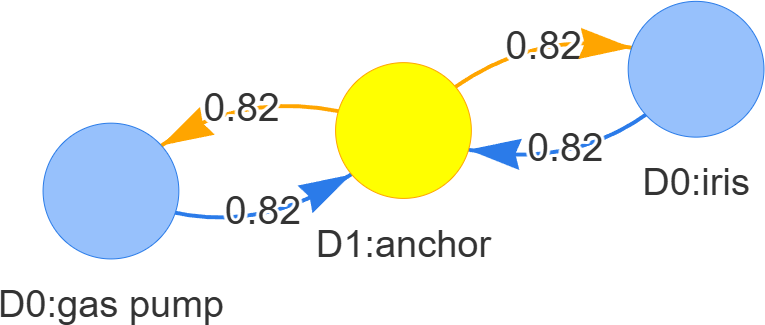
\includegraphics[width=0.35\textwidth]{figures/wordnet.png}

      \caption{An example of a bad WordNet cluster in a relationship graph between Caltech256 and Caltech101.
            These false positives occur commonly and make WordNet unsuitable as a ground truth taxonomy.}
      \label{fig:wordnet}
\end{figure}

Upon further observation, this problem turns out to be even more severe:
WordNet's synsets build relations based on usage patterns in text corpora,
which does not align with our visual relationships based on shared concepts and attributes.
In Figure~\ref{fig:wordnet}, we see a relationship cluster with the classes \textit{gas pump}, \textit{anchor} and \textit{iris}.
These words do not share any visual similarities or attributes, yet they are clustered together based on their textual relationships
(we guess that \textit{gas pump} and \textit{anchor} are related through their usage in similar contexts like ships and maritime activities).
Unfortunately upon manual inspection, these false positives occur frequently.

Since we try to build a ground truth taxonomy to evaluate relationship selection methods,
these false positives can significantly skew the results and make WordNet unsuitable for our purposes.

\subsubsection{Alternate Evaluation Methods - SVHN-MNIST}

Next, we try to use the SVHN and MNIST datasets to create a relationship graph.
These datasets provide a special usability for our purposes,
since the relationships between the classes can be manually defined.
Also, since the datasets have a sufficiently shifted domain (i.e. drawn, greyscale images vs. real-world images of house numbers
from different angles, lighting conditions, etc.),
the differences are large enough to make the task of relationship selection more difficult and realistic.

\begin{figure}[ht]
      \centering
      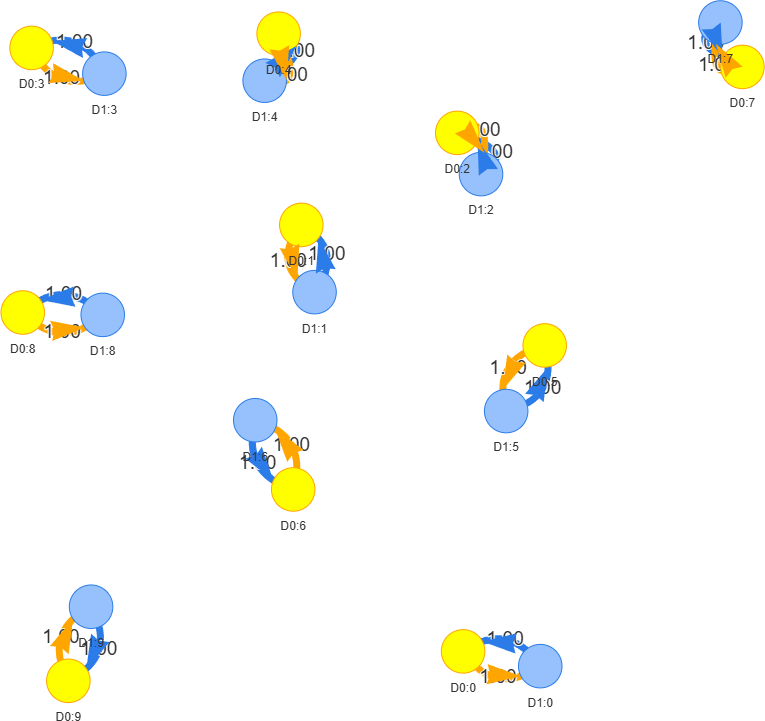
\includegraphics[width=0.35\textwidth]{figures/svhn_mnist.png}

      \caption{This figure shows the complete relationship graph between the SVHN and MNIST datasets.
            The relationships are unequivocal and straightforward, as the classes are identical across both datasets;
            however, they lack complexity.}
      \label{fig:svhn_mnist}
\end{figure}

In Figure~\ref{fig:svhn_mnist}, we can see the complete relationship graph between the SVHN and MNIST datasets.
Every relationship is a simple connection between two classes with a weight of 1.0.

While we could rerun our relationship selection method evaluation on this taxonomy,
we decide against this method upon further reflection:
\begin{itemize}
      \item Real-world taxonomies will not be made up of single, isolated relationships
            with a weight of 1.0. Complex subsets, mismatches or overlaps between classes are completely missing.
      \item This taxonomy will have only ten universal classes, which makes the sample size too small to draw meaningful conclusions.
      \item Our previous datasets contained a wide range of general-purpose classes as well as more specific ones, which allowed for a more nuanced evaluation of our methods.
            This taxonomy will be limited to numbers.
\end{itemize}

\subsubsection{Alternate Evaluation Methods - Domain-Shift Synthetic Datasets}

The main advantage of our synthetic dataset variants is their ability to create a proven correct ground truth taxonomy.
Instead of trying to derive a ground truth using new, suboptimal methods,
we instead try to fix the underlying issues with our existing method.

Our synthetic variants contain the same underlying images,
which result in a near-perfect, unrealistic cross-domain model prediction accuracy.
Due to this high model confidence, the best performing relationship selection methods are likely to be overly optimistic
and therefore perform poorly in real-world scenarios where models will not be able to perform as well across domains.


\begin{figure}[ht]
      \centering
      \includegraphics[width=\textwidth]{figures/domain_shift_visualization.png}

      \caption{Example images from the domain-shifted synthetic variants.
            We apply different transformations to the images of the original synthetic dataset
            to create two new domains. The first domain (Domain A) is a noisy greyscale variant,
            while the second domain (Domain B) is a rotated, blurry version of the original images,
            and the third domain (Domain C) has random erasings, shifted perspectives, and color jitter.}
      \label{fig:domain_shift}
\end{figure}

To mitigate this issue, we try to synthetically create a different domain for each variant by applying transforms to the
underlying dataset images.
An example subset of the domain-shifted images is shown in Figure~\ref{fig:domain_shift}:
Using different transforms, the images appear in unique styles and distortions,
synthetically changing their visual characteristics
while retaining the same classes and relationships.

\begin{table}[ht]
\centering
\caption{Evaluation results on test sets for domain-shifted experiments. Models were trained with different domain shift transformations and checkpointed after every epoch. The model with the lowest validation loss was selected for evaluation on the test set.}
\label{tab:evaluation_results_domain_shifted}
\begin{tabular}{cccc}
\toprule
Dataset Variant & Domain & Steps & Accuracy \\
\midrule
Caltech-256 2-Domain Domain Shifted Variant 1 & A & 13800 & 0.72 \\
Caltech-256 2-Domain Domain Shifted Variant 1 & B & 13050 & 0.76 \\
Caltech-256 2-Domain Domain Shifted Variant 2 & A & 14450 & 0.70 \\
Caltech-256 2-Domain Domain Shifted Variant 2 & B & 14700 & 0.75 \\
Caltech-256 3-Domain Domain Shifted Variant & A & 13800 & 0.70 \\
Caltech-256 3-Domain Domain Shifted Variant & B & 13750 & 0.75 \\
Caltech-256 3-Domain Domain Shifted Variant & C & 12350 & 0.74 \\
CIFAR-100 2-Domain Domain Shifted Variant & A & 8200 & 0.57 \\
CIFAR-100 2-Domain Domain Shifted Variant & B & 7900 & 0.63 \\
\bottomrule
\end{tabular}
\end{table}

\begin{table}[ht]
\centering
\caption{Average performance metrics for relationship discovery methods with globally optimal parameters on domain-shifted experiments. Each method uses the parameter value that minimizes the average EDR across all domain-shifted dataset variants. Performance metrics are then averaged across all dataset variants using these optimal parameters.}
\label{tab:relationship_methods_global_optimal_domain_shifted}
\begin{tabular}{lccccc}
\toprule
Method & Parameter & EDR & Precision & Recall & F1-score \\
\midrule
MCFP & N/A & 0.842 & \textbf{0.490} & 0.226 & 0.305 \\
Naive Thresholding & 0.10 & 0.761 & 0.418 & 0.519 & \textbf{0.450} \\
Density Thresholding & 0.60 & 0.766 & 0.349 & \textbf{0.582} & 0.426 \\
Relationship Hypothesis & 5 & \textbf{0.759} & 0.390 & 0.543 & 0.444 \\
\bottomrule
\end{tabular}
\end{table}


The training performance of these new domain-shifted models can be seen in Table~\ref{tab:evaluation_results_domain_shifted}.
We can observe a $10\%$ decrease in accuracy on the test data compared to the original synthetic dataset variants.
This was to be expected due to the increased complexity of the domain-shifted tasks.

When comparing the new averaged relationship method evaluation results in Table~\ref{tab:relationship_methods_global_optimal_domain_shifted}
to our original non-domain-shifted results in Table~\ref{tab:relationship_methods_global_optimal},
we can observe significant differences:

\begin{itemize}
      \item Our new best performing relationship selection method,
            based on averaged maximum EDR scores, changes from MCFP to the relationship hypothesis method.
      \item In general, all methods have a lower EDR score than their non-domain-shifted counterparts.
            This is a direct result of the decreased domain model accuracy and was to be expected.
      \item The MCFP method still has the highest relative precision with $0.49$.
            If precision is more important than EDR for a high universal model accuracy
            will be evaluated in the universal model training section (see Section~\ref{sec:universal_models}).
\end{itemize}

We will use the most promising relationship selection methods,
MCFP and relationship hypothesis, for our universal model training.
Our final evaluation will focus on the model accuracy of the trained universal Models
built with the universal taxonomies of the two preselected relationship selection methods
(using the selection method parameters that have the best EDR score).

\subsection{Universal Taxonomy Generation}

\begin{figure}[ht]
      \centering
      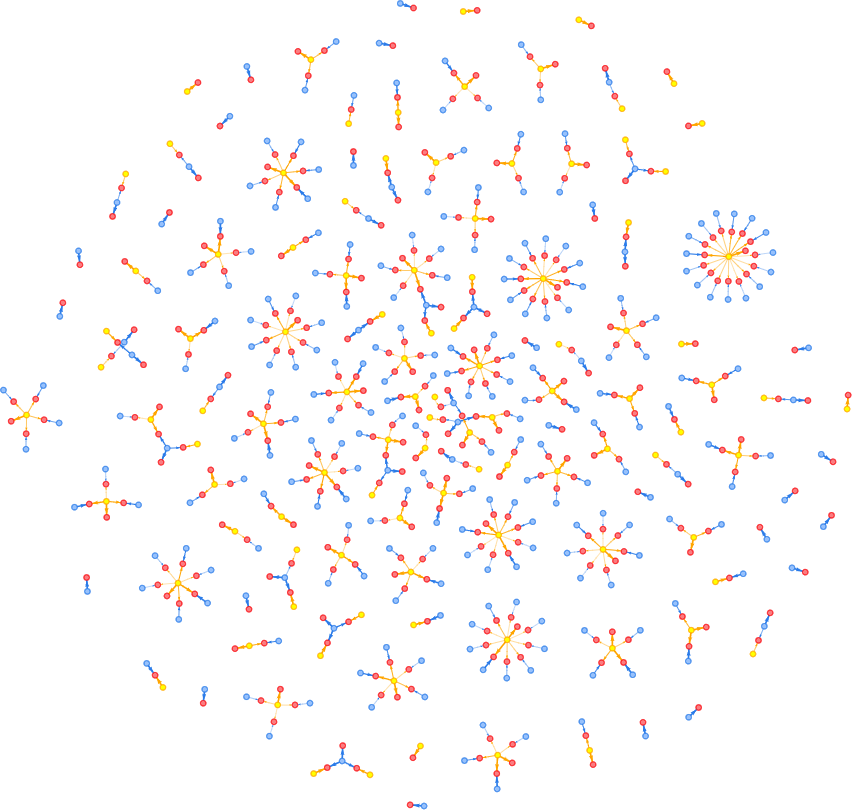
\includegraphics[width=0.35\textwidth]{figures/taxonomy.png}

      \caption{This figure shows the complete Caltech101-Caltech256 universal taxonomy.
            While most classes build smaller clusters build smaller clusters of 2-3 classes,
            some large clusters can be observed.}
      \label{fig:taxonomy}
\end{figure}

\begin{figure}[ht]
      \centering
      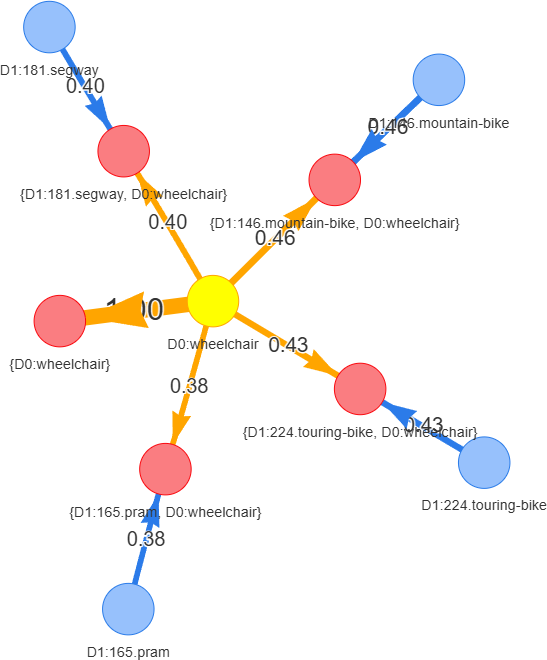
\includegraphics[width=0.35\textwidth]{figures/wheel_concept.png}

      \caption{In the Caltech101-Caltech256 universal taxonomy,
            this cluster only contains vehicles. The universal classes created can be interpreted as
            sharing a common concept of \enquote{wheel}.}
      \label{fig:wheel_concept}
\end{figure}

\begin{figure}[ht]
      \centering
      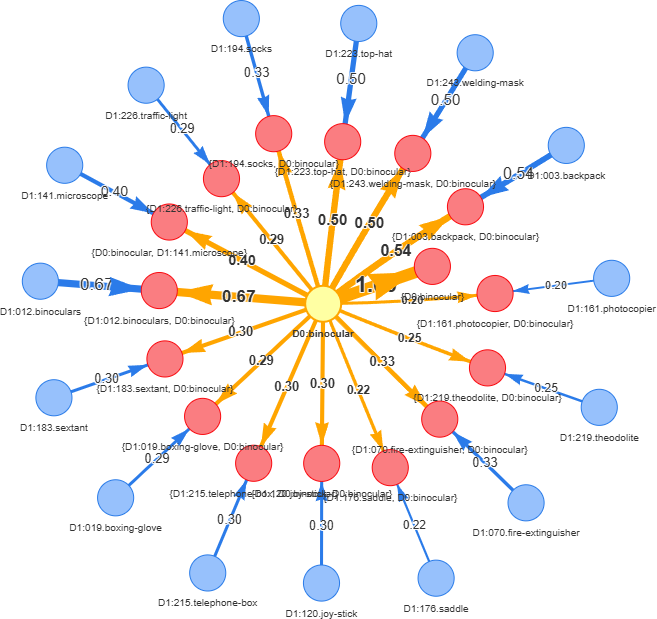
\includegraphics[width=0.35\textwidth]{figures/bad_taxonomy.png}

      \caption{This example in the Caltech101-Caltech256 universal taxonomy shows a wrong relationship
            cluster towards the Caltech101 class \enquote{binocular}. Many of the Caltech256 classes
            do not have a suitable representation in the Caltech101 dataset
            and then connect to the Caltech101 class \enquote{binocular} instead.}
      \label{fig:bad_taxonomy}
\end{figure}

We now have our domain models trained and our relationship selection methods evaluated.
In the next step, we run our universal taxonomy generation algorithm
(see Section~\ref{sec:universal_taxonomy_algorithm}) on the Caltech-101 and
Caltech-256 datasets. To make the results more interpretable,
we will use the most common foreign prediction method to have a sparse relationship graph
that is easier to look at
(for our later universal model training, we will of course work with both the naive thresholding method and the most common foreign prediction method).

The overall universal taxonomy generated from the Caltech-101 and Caltech-256 datasets
is shown in Figure~\ref{fig:taxonomy}.
We can observe many smaller clusters of 2-3 classes which build from a single domain class in
the Caltech-101 dataset and multiple domain classes in the Caltech-256 dataset
(since the Caltech-256 dataset has more granular classes, this is to be expected).

An example of a \enquote{good} cluster is shown in Figure~\ref{fig:wheel_concept}:
This cluster centers around the Caltech101 class \enquote{wheelchair} and contains
multiple Caltech256 classes that share the concept of \enquote{wheel} (e.g. \enquote{mountain bike}, \enquote{segway}, \enquote{touring bike}, etc.).
The universal classes between the Caltech101 and Caltech256 classes
will provide a useful mapping for our universal model training.

However, we can also observe \enquote{bad} clusters in the universal taxonomy,
such as the one shown in Figure~\ref{fig:bad_taxonomy}:
The Caltech101 class \enquote{binocular} is connected to multiple Caltech256 classes
of a variety of different concepts.
While many of these classes do share concepts with binoculars (e.g. \enquote{sextant}, \enquote{telescope}, etc.),
many of the Caltech256 classes in the cluster do not have an obvious connection to binoculars
(e.g. \enquote{boxing glove}, \enquote{fire extinguisher}, etc.).
Since it is likely that the Caltech256 dataset contains classes that do not have a suitable representation in the Caltech101 dataset,
we \enquote{force} a relationship to a Caltech101 class by using the most common foreign prediction method.
However, the incorrect relationships do have a low relationship weight which makes
the error less severe for the universal model training.

Addressing these issues is a complex task, since a suitable threshold for the relationship weights
depends on the individual composition of the datasets.


\section{Universal Models} \label{sec:universal_models}

\subsection{Training}

\subsubsection{Modifications to Baseline Architecture}

Building upon the ResNet-50 architecture used for the individual domain models, we developed a \texttt{UniversalResNetModel} that incorporates several key modifications to enable multi-domain training through our universal taxonomy approach.

The most significant architectural change is the replacement of the standard classification head. While the baseline \texttt{ResNetModel} uses a multi-layer fully connected classifier with dropout regularization that outputs logits for domain-specific classes, the \texttt{UniversalResNetModel} employs a simplified two-layer fully connected head that outputs logits for universal classes:

\begin{itemize}
      \item \textbf{Baseline classifier}: A 6-layer fully connected network with dropout (0.5, 0.2, 0.2, 0.2, 0.2) that progressively reduces dimensionality from ResNet features $\rightarrow$ 1024 $\rightarrow$ 512 $\rightarrow$ 256 $\rightarrow$ 128 $\rightarrow$ domain classes
      \item \textbf{Universal classifier}: A 2-layer fully connected network (ResNet features $\rightarrow$ 1024 $\rightarrow$ universal classes) without dropout regularization
\end{itemize}

The simplified architecture proved to be more effective in training runs vs. the more complex hopper + dropout architecture used in the baseline models.

Another crucial modification is the loss function:
The baseline models use standard cross-entropy loss with one-hot encoded targets,
while the universal model employs cross-entropy for discrete probability distributions for a loss function.
This change accommodates the fact that domain classes may map to multiple universal classes with different weights,
as determined by the taxonomy relationships
(full explanation in Section~\ref{sec:universal_model_learning}).

\subsubsection{Multi-Domain Training Procedure}

Instead of training separate models on individual datasets,
we create a new combined dataset that merges multiple datasets while preserving domain identity.
Each training sample is augmented with a domain identifier,
transforming the standard $(\texttt{image}, \texttt{label})$ pairs into $(\texttt{image}, (\texttt{domain\_id}, \texttt{label}))$ tuples.
This allows the model to handle samples from different datasets within the same batch
(since we need to know the image domain to apply the correct target mapping).

During training experiments, the validation loss starts to increase again after a few epochs, indicating potential overfitting.
However, the validation accuracy continues to improve, suggesting that the model is still learning useful features.
To still use the best performing model checkpoint, we change checkpointing to monitor validation accuracy instead of validation loss.

This seemingly contradictory behavior of rising validation loss with rising validation accuracy can be explained by several factors:

\begin{itemize}
      \item \textbf{Multi-target probability distributions}: Unlike standard classification with one-hot targets,
            our universal model uses discrete probability distributions as targets.
            The model may be learning to better predict the correct class ranks while becoming less confident about exact probability values,
            leading to higher cross-entropy loss but better top-1 accuracy.
      \item \textbf{Label smoothing}: The universal taxonomy creates implicit
            label smoothing effects where domain classes map to multiple universal classes
            with different weights.
            For perfect accuracy across all domains, it might not be possible to also hit
            the exact probability values, leading to higher loss \textit{and} higher accuracy simultaneously
            while training.
      \item \textbf{Learning dynamics}: The model may be transitioning
            from overfitting to individual domain patterns toward learning more generalisable
            universal features, causing higher loss when switching between phases of learning.
\end{itemize}

As a final note on the training procedure,
we rescale the CIFAR-100 images to match the size of the other datasets (224x224 pixels),
so that we can process all images uniformly in the same model architecture.

\subsection{Performance}

\begin{table}[ht]
\centering
\caption{Baseline ResNet model performance on individual datasets. These single-domain models serve as reference points for evaluating the universal models. Every baseline model was trained for 50 epochs.}
\label{tab:baseline_model_results}
\begin{tabular}{lccc}
\toprule
Dataset & Architecture & Optimizer & Test Accuracy \\
\midrule
Caltech-101 & ResNet-50 & SGD & 90.54 \\
Caltech-256 & ResNet-50 & AdamW & 69.54 \\
CIFAR-100 & ResNet-152 & AdamW & 60.48 \\
\bottomrule
\end{tabular}
\end{table}

\begin{table}[ht]
\centering
\caption{Universal model evaluation results on multi-domain test datasets. Two-domain models were trained on Caltech-101 + Caltech-256, while three-domain models were trained on all three datasets. Models were evaluated on individual domains as well as the combined test set (no weighting was applied, the individual test sets were simply concatenated). Domain accuracy values show performance differences compared to single-domain baseline models (see Table~\ref{tab:baseline_model_results}). Best results per column are shown in bold. All accuracy values are shown as percentages. Density Threshold models use parameter 0.6, Naive Threshold models use parameter 0.1.}
\label{tab:universal_model_results}
\begin{tabular}{lcccc}
\toprule
Taxonomy & Caltech-101 & Caltech-256 & CIFAR-100 & Avg \\
\midrule
Hypothesis (2 Domain) & 92.16 (-0.00) & 82.48 (+12.22) & N/A & 84.34 \\
MCFP (2 Domain) & 90.77 (-1.39) & 80.75 (+10.49) & N/A & 82.63 \\
MCFP Binary (2 Domain) & 92.73 (+0.57) & \textbf{90.33 (+20.07)} & N/A & 90.25 \\
Density Threshold (2 Domain) & 92.39 (+0.23) & 81.31 (+11.05) & N/A & 83.42 \\
Naive Threshold (2 Domain) & 94.35 (+2.19) & 82.12 (+11.86) & N/A & 84.52 \\
Hypothesis (3 Domain) & 69.55 (-22.61) & 58.24 (-12.02) & 69.03 (+8.55) & 66.72 \\
MCFP (3 Domain) & 82.58 (-9.58) & 76.80 (+6.54) & 76.10 (+15.62) & 76.69 \\
MCFP Binary (3 Domain) & 93.77 (+1.61) & 85.33 (+15.07) & 82.71 (+22.23) & 83.92 \\
Density Threshold (3 Domain) & \textbf{95.39 (+3.23)} & 83.04 (+12.78) & \textbf{83.14 (+22.66)} & 83.97 \\
Naive Threshold (3 Domain) & 95.39 (+3.23) & 86.31 (+16.05) & 72.56 (+12.08) & 76.92 \\
\bottomrule
\end{tabular}
\end{table}


\begin{figure}[ht]
      \centering
      \scalebox{0.35}{%% Creator: Matplotlib, PGF backend
%%
%% To include the figure in your LaTeX document, write
%%   \input{<filename>.pgf}
%%
%% Make sure the required packages are loaded in your preamble
%%   \usepackage{pgf}
%%
%% Also ensure that all the required font packages are loaded; for instance,
%% the lmodern package is sometimes necessary when using math font.
%%   \usepackage{lmodern}
%%
%% Figures using additional raster images can only be included by \input if
%% they are in the same directory as the main LaTeX file. For loading figures
%% from other directories you can use the `import` package
%%   \usepackage{import}
%%
%% and then include the figures with
%%   \import{<path to file>}{<filename>.pgf}
%%
%% Matplotlib used the following preamble
%%   \def\mathdefault#1{#1}
%%   \everymath=\expandafter{\the\everymath\displaystyle}
%%   \IfFileExists{scrextend.sty}{
%%     \usepackage[fontsize=11.000000pt]{scrextend}
%%   }{
%%     \renewcommand{\normalsize}{\fontsize{11.000000}{13.200000}\selectfont}
%%     \normalsize
%%   }
%%   
%%   \ifdefined\pdftexversion\else  % non-pdftex case.
%%     \usepackage{fontspec}
%%     \setmainfont{DejaVuSerif.ttf}[Path=\detokenize{/home/bjoern/miniconda3/envs/master-thesis/lib/python3.13/site-packages/matplotlib/mpl-data/fonts/ttf/}]
%%     \setsansfont{DejaVuSans.ttf}[Path=\detokenize{/home/bjoern/miniconda3/envs/master-thesis/lib/python3.13/site-packages/matplotlib/mpl-data/fonts/ttf/}]
%%     \setmonofont{DejaVuSansMono.ttf}[Path=\detokenize{/home/bjoern/miniconda3/envs/master-thesis/lib/python3.13/site-packages/matplotlib/mpl-data/fonts/ttf/}]
%%   \fi
%%   \makeatletter\@ifpackageloaded{underscore}{}{\usepackage[strings]{underscore}}\makeatother
%%
\begingroup%
\makeatletter%
\begin{pgfpicture}%
\pgfpathrectangle{\pgfpointorigin}{\pgfqpoint{14.841618in}{9.870000in}}%
\pgfusepath{use as bounding box, clip}%
\begin{pgfscope}%
\pgfsetbuttcap%
\pgfsetmiterjoin%
\definecolor{currentfill}{rgb}{1.000000,1.000000,1.000000}%
\pgfsetfillcolor{currentfill}%
\pgfsetlinewidth{0.000000pt}%
\definecolor{currentstroke}{rgb}{1.000000,1.000000,1.000000}%
\pgfsetstrokecolor{currentstroke}%
\pgfsetdash{}{0pt}%
\pgfpathmoveto{\pgfqpoint{0.000000in}{0.000000in}}%
\pgfpathlineto{\pgfqpoint{14.841618in}{0.000000in}}%
\pgfpathlineto{\pgfqpoint{14.841618in}{9.870000in}}%
\pgfpathlineto{\pgfqpoint{0.000000in}{9.870000in}}%
\pgfpathlineto{\pgfqpoint{0.000000in}{0.000000in}}%
\pgfpathclose%
\pgfusepath{fill}%
\end{pgfscope}%
\begin{pgfscope}%
\pgfsetbuttcap%
\pgfsetmiterjoin%
\definecolor{currentfill}{rgb}{1.000000,1.000000,1.000000}%
\pgfsetfillcolor{currentfill}%
\pgfsetlinewidth{0.000000pt}%
\definecolor{currentstroke}{rgb}{0.000000,0.000000,0.000000}%
\pgfsetstrokecolor{currentstroke}%
\pgfsetstrokeopacity{0.000000}%
\pgfsetdash{}{0pt}%
\pgfpathmoveto{\pgfqpoint{0.598357in}{5.472778in}}%
\pgfpathlineto{\pgfqpoint{7.324118in}{5.472778in}}%
\pgfpathlineto{\pgfqpoint{7.324118in}{9.557417in}}%
\pgfpathlineto{\pgfqpoint{0.598357in}{9.557417in}}%
\pgfpathlineto{\pgfqpoint{0.598357in}{5.472778in}}%
\pgfpathclose%
\pgfusepath{fill}%
\end{pgfscope}%
\begin{pgfscope}%
\pgfpathrectangle{\pgfqpoint{0.598357in}{5.472778in}}{\pgfqpoint{6.725761in}{4.084639in}}%
\pgfusepath{clip}%
\pgfsetrectcap%
\pgfsetroundjoin%
\pgfsetlinewidth{0.803000pt}%
\definecolor{currentstroke}{rgb}{0.690196,0.690196,0.690196}%
\pgfsetstrokecolor{currentstroke}%
\pgfsetstrokeopacity{0.300000}%
\pgfsetdash{}{0pt}%
\pgfpathmoveto{\pgfqpoint{0.891869in}{5.472778in}}%
\pgfpathlineto{\pgfqpoint{0.891869in}{9.557417in}}%
\pgfusepath{stroke}%
\end{pgfscope}%
\begin{pgfscope}%
\pgfsetbuttcap%
\pgfsetroundjoin%
\definecolor{currentfill}{rgb}{0.000000,0.000000,0.000000}%
\pgfsetfillcolor{currentfill}%
\pgfsetlinewidth{0.803000pt}%
\definecolor{currentstroke}{rgb}{0.000000,0.000000,0.000000}%
\pgfsetstrokecolor{currentstroke}%
\pgfsetdash{}{0pt}%
\pgfsys@defobject{currentmarker}{\pgfqpoint{0.000000in}{-0.048611in}}{\pgfqpoint{0.000000in}{0.000000in}}{%
\pgfpathmoveto{\pgfqpoint{0.000000in}{0.000000in}}%
\pgfpathlineto{\pgfqpoint{0.000000in}{-0.048611in}}%
\pgfusepath{stroke,fill}%
}%
\begin{pgfscope}%
\pgfsys@transformshift{0.891869in}{5.472778in}%
\pgfsys@useobject{currentmarker}{}%
\end{pgfscope}%
\end{pgfscope}%
\begin{pgfscope}%
\definecolor{textcolor}{rgb}{0.000000,0.000000,0.000000}%
\pgfsetstrokecolor{textcolor}%
\pgfsetfillcolor{textcolor}%
\pgftext[x=0.891869in,y=5.375556in,,top]{\color{textcolor}{\ifdefined\pdftexversion\else\setmainfont{EB Garamond}\rmfamily\fi\fontsize{11.000000}{13.200000}\selectfont\catcode`\^=\active\def^{\ifmmode\sp\else\^{}\fi}\catcode`\%=\active\def%{\%}$\mathdefault{0}$}}%
\end{pgfscope}%
\begin{pgfscope}%
\pgfpathrectangle{\pgfqpoint{0.598357in}{5.472778in}}{\pgfqpoint{6.725761in}{4.084639in}}%
\pgfusepath{clip}%
\pgfsetrectcap%
\pgfsetroundjoin%
\pgfsetlinewidth{0.803000pt}%
\definecolor{currentstroke}{rgb}{0.690196,0.690196,0.690196}%
\pgfsetstrokecolor{currentstroke}%
\pgfsetstrokeopacity{0.300000}%
\pgfsetdash{}{0pt}%
\pgfpathmoveto{\pgfqpoint{2.137150in}{5.472778in}}%
\pgfpathlineto{\pgfqpoint{2.137150in}{9.557417in}}%
\pgfusepath{stroke}%
\end{pgfscope}%
\begin{pgfscope}%
\pgfsetbuttcap%
\pgfsetroundjoin%
\definecolor{currentfill}{rgb}{0.000000,0.000000,0.000000}%
\pgfsetfillcolor{currentfill}%
\pgfsetlinewidth{0.803000pt}%
\definecolor{currentstroke}{rgb}{0.000000,0.000000,0.000000}%
\pgfsetstrokecolor{currentstroke}%
\pgfsetdash{}{0pt}%
\pgfsys@defobject{currentmarker}{\pgfqpoint{0.000000in}{-0.048611in}}{\pgfqpoint{0.000000in}{0.000000in}}{%
\pgfpathmoveto{\pgfqpoint{0.000000in}{0.000000in}}%
\pgfpathlineto{\pgfqpoint{0.000000in}{-0.048611in}}%
\pgfusepath{stroke,fill}%
}%
\begin{pgfscope}%
\pgfsys@transformshift{2.137150in}{5.472778in}%
\pgfsys@useobject{currentmarker}{}%
\end{pgfscope}%
\end{pgfscope}%
\begin{pgfscope}%
\definecolor{textcolor}{rgb}{0.000000,0.000000,0.000000}%
\pgfsetstrokecolor{textcolor}%
\pgfsetfillcolor{textcolor}%
\pgftext[x=2.137150in,y=5.375556in,,top]{\color{textcolor}{\ifdefined\pdftexversion\else\setmainfont{EB Garamond}\rmfamily\fi\fontsize{11.000000}{13.200000}\selectfont\catcode`\^=\active\def^{\ifmmode\sp\else\^{}\fi}\catcode`\%=\active\def%{\%}$\mathdefault{5000}$}}%
\end{pgfscope}%
\begin{pgfscope}%
\pgfpathrectangle{\pgfqpoint{0.598357in}{5.472778in}}{\pgfqpoint{6.725761in}{4.084639in}}%
\pgfusepath{clip}%
\pgfsetrectcap%
\pgfsetroundjoin%
\pgfsetlinewidth{0.803000pt}%
\definecolor{currentstroke}{rgb}{0.690196,0.690196,0.690196}%
\pgfsetstrokecolor{currentstroke}%
\pgfsetstrokeopacity{0.300000}%
\pgfsetdash{}{0pt}%
\pgfpathmoveto{\pgfqpoint{3.382431in}{5.472778in}}%
\pgfpathlineto{\pgfqpoint{3.382431in}{9.557417in}}%
\pgfusepath{stroke}%
\end{pgfscope}%
\begin{pgfscope}%
\pgfsetbuttcap%
\pgfsetroundjoin%
\definecolor{currentfill}{rgb}{0.000000,0.000000,0.000000}%
\pgfsetfillcolor{currentfill}%
\pgfsetlinewidth{0.803000pt}%
\definecolor{currentstroke}{rgb}{0.000000,0.000000,0.000000}%
\pgfsetstrokecolor{currentstroke}%
\pgfsetdash{}{0pt}%
\pgfsys@defobject{currentmarker}{\pgfqpoint{0.000000in}{-0.048611in}}{\pgfqpoint{0.000000in}{0.000000in}}{%
\pgfpathmoveto{\pgfqpoint{0.000000in}{0.000000in}}%
\pgfpathlineto{\pgfqpoint{0.000000in}{-0.048611in}}%
\pgfusepath{stroke,fill}%
}%
\begin{pgfscope}%
\pgfsys@transformshift{3.382431in}{5.472778in}%
\pgfsys@useobject{currentmarker}{}%
\end{pgfscope}%
\end{pgfscope}%
\begin{pgfscope}%
\definecolor{textcolor}{rgb}{0.000000,0.000000,0.000000}%
\pgfsetstrokecolor{textcolor}%
\pgfsetfillcolor{textcolor}%
\pgftext[x=3.382431in,y=5.375556in,,top]{\color{textcolor}{\ifdefined\pdftexversion\else\setmainfont{EB Garamond}\rmfamily\fi\fontsize{11.000000}{13.200000}\selectfont\catcode`\^=\active\def^{\ifmmode\sp\else\^{}\fi}\catcode`\%=\active\def%{\%}$\mathdefault{10000}$}}%
\end{pgfscope}%
\begin{pgfscope}%
\pgfpathrectangle{\pgfqpoint{0.598357in}{5.472778in}}{\pgfqpoint{6.725761in}{4.084639in}}%
\pgfusepath{clip}%
\pgfsetrectcap%
\pgfsetroundjoin%
\pgfsetlinewidth{0.803000pt}%
\definecolor{currentstroke}{rgb}{0.690196,0.690196,0.690196}%
\pgfsetstrokecolor{currentstroke}%
\pgfsetstrokeopacity{0.300000}%
\pgfsetdash{}{0pt}%
\pgfpathmoveto{\pgfqpoint{4.627711in}{5.472778in}}%
\pgfpathlineto{\pgfqpoint{4.627711in}{9.557417in}}%
\pgfusepath{stroke}%
\end{pgfscope}%
\begin{pgfscope}%
\pgfsetbuttcap%
\pgfsetroundjoin%
\definecolor{currentfill}{rgb}{0.000000,0.000000,0.000000}%
\pgfsetfillcolor{currentfill}%
\pgfsetlinewidth{0.803000pt}%
\definecolor{currentstroke}{rgb}{0.000000,0.000000,0.000000}%
\pgfsetstrokecolor{currentstroke}%
\pgfsetdash{}{0pt}%
\pgfsys@defobject{currentmarker}{\pgfqpoint{0.000000in}{-0.048611in}}{\pgfqpoint{0.000000in}{0.000000in}}{%
\pgfpathmoveto{\pgfqpoint{0.000000in}{0.000000in}}%
\pgfpathlineto{\pgfqpoint{0.000000in}{-0.048611in}}%
\pgfusepath{stroke,fill}%
}%
\begin{pgfscope}%
\pgfsys@transformshift{4.627711in}{5.472778in}%
\pgfsys@useobject{currentmarker}{}%
\end{pgfscope}%
\end{pgfscope}%
\begin{pgfscope}%
\definecolor{textcolor}{rgb}{0.000000,0.000000,0.000000}%
\pgfsetstrokecolor{textcolor}%
\pgfsetfillcolor{textcolor}%
\pgftext[x=4.627711in,y=5.375556in,,top]{\color{textcolor}{\ifdefined\pdftexversion\else\setmainfont{EB Garamond}\rmfamily\fi\fontsize{11.000000}{13.200000}\selectfont\catcode`\^=\active\def^{\ifmmode\sp\else\^{}\fi}\catcode`\%=\active\def%{\%}$\mathdefault{15000}$}}%
\end{pgfscope}%
\begin{pgfscope}%
\pgfpathrectangle{\pgfqpoint{0.598357in}{5.472778in}}{\pgfqpoint{6.725761in}{4.084639in}}%
\pgfusepath{clip}%
\pgfsetrectcap%
\pgfsetroundjoin%
\pgfsetlinewidth{0.803000pt}%
\definecolor{currentstroke}{rgb}{0.690196,0.690196,0.690196}%
\pgfsetstrokecolor{currentstroke}%
\pgfsetstrokeopacity{0.300000}%
\pgfsetdash{}{0pt}%
\pgfpathmoveto{\pgfqpoint{5.872992in}{5.472778in}}%
\pgfpathlineto{\pgfqpoint{5.872992in}{9.557417in}}%
\pgfusepath{stroke}%
\end{pgfscope}%
\begin{pgfscope}%
\pgfsetbuttcap%
\pgfsetroundjoin%
\definecolor{currentfill}{rgb}{0.000000,0.000000,0.000000}%
\pgfsetfillcolor{currentfill}%
\pgfsetlinewidth{0.803000pt}%
\definecolor{currentstroke}{rgb}{0.000000,0.000000,0.000000}%
\pgfsetstrokecolor{currentstroke}%
\pgfsetdash{}{0pt}%
\pgfsys@defobject{currentmarker}{\pgfqpoint{0.000000in}{-0.048611in}}{\pgfqpoint{0.000000in}{0.000000in}}{%
\pgfpathmoveto{\pgfqpoint{0.000000in}{0.000000in}}%
\pgfpathlineto{\pgfqpoint{0.000000in}{-0.048611in}}%
\pgfusepath{stroke,fill}%
}%
\begin{pgfscope}%
\pgfsys@transformshift{5.872992in}{5.472778in}%
\pgfsys@useobject{currentmarker}{}%
\end{pgfscope}%
\end{pgfscope}%
\begin{pgfscope}%
\definecolor{textcolor}{rgb}{0.000000,0.000000,0.000000}%
\pgfsetstrokecolor{textcolor}%
\pgfsetfillcolor{textcolor}%
\pgftext[x=5.872992in,y=5.375556in,,top]{\color{textcolor}{\ifdefined\pdftexversion\else\setmainfont{EB Garamond}\rmfamily\fi\fontsize{11.000000}{13.200000}\selectfont\catcode`\^=\active\def^{\ifmmode\sp\else\^{}\fi}\catcode`\%=\active\def%{\%}$\mathdefault{20000}$}}%
\end{pgfscope}%
\begin{pgfscope}%
\pgfpathrectangle{\pgfqpoint{0.598357in}{5.472778in}}{\pgfqpoint{6.725761in}{4.084639in}}%
\pgfusepath{clip}%
\pgfsetrectcap%
\pgfsetroundjoin%
\pgfsetlinewidth{0.803000pt}%
\definecolor{currentstroke}{rgb}{0.690196,0.690196,0.690196}%
\pgfsetstrokecolor{currentstroke}%
\pgfsetstrokeopacity{0.300000}%
\pgfsetdash{}{0pt}%
\pgfpathmoveto{\pgfqpoint{7.118273in}{5.472778in}}%
\pgfpathlineto{\pgfqpoint{7.118273in}{9.557417in}}%
\pgfusepath{stroke}%
\end{pgfscope}%
\begin{pgfscope}%
\pgfsetbuttcap%
\pgfsetroundjoin%
\definecolor{currentfill}{rgb}{0.000000,0.000000,0.000000}%
\pgfsetfillcolor{currentfill}%
\pgfsetlinewidth{0.803000pt}%
\definecolor{currentstroke}{rgb}{0.000000,0.000000,0.000000}%
\pgfsetstrokecolor{currentstroke}%
\pgfsetdash{}{0pt}%
\pgfsys@defobject{currentmarker}{\pgfqpoint{0.000000in}{-0.048611in}}{\pgfqpoint{0.000000in}{0.000000in}}{%
\pgfpathmoveto{\pgfqpoint{0.000000in}{0.000000in}}%
\pgfpathlineto{\pgfqpoint{0.000000in}{-0.048611in}}%
\pgfusepath{stroke,fill}%
}%
\begin{pgfscope}%
\pgfsys@transformshift{7.118273in}{5.472778in}%
\pgfsys@useobject{currentmarker}{}%
\end{pgfscope}%
\end{pgfscope}%
\begin{pgfscope}%
\definecolor{textcolor}{rgb}{0.000000,0.000000,0.000000}%
\pgfsetstrokecolor{textcolor}%
\pgfsetfillcolor{textcolor}%
\pgftext[x=7.118273in,y=5.375556in,,top]{\color{textcolor}{\ifdefined\pdftexversion\else\setmainfont{EB Garamond}\rmfamily\fi\fontsize{11.000000}{13.200000}\selectfont\catcode`\^=\active\def^{\ifmmode\sp\else\^{}\fi}\catcode`\%=\active\def%{\%}$\mathdefault{25000}$}}%
\end{pgfscope}%
\begin{pgfscope}%
\definecolor{textcolor}{rgb}{0.000000,0.000000,0.000000}%
\pgfsetstrokecolor{textcolor}%
\pgfsetfillcolor{textcolor}%
\pgftext[x=3.961237in,y=5.168750in,,top]{\color{textcolor}{\ifdefined\pdftexversion\else\setmainfont{EB Garamond}\rmfamily\fi\fontsize{11.000000}{13.200000}\selectfont\catcode`\^=\active\def^{\ifmmode\sp\else\^{}\fi}\catcode`\%=\active\def%{\%}Steps}}%
\end{pgfscope}%
\begin{pgfscope}%
\pgfpathrectangle{\pgfqpoint{0.598357in}{5.472778in}}{\pgfqpoint{6.725761in}{4.084639in}}%
\pgfusepath{clip}%
\pgfsetrectcap%
\pgfsetroundjoin%
\pgfsetlinewidth{0.803000pt}%
\definecolor{currentstroke}{rgb}{0.690196,0.690196,0.690196}%
\pgfsetstrokecolor{currentstroke}%
\pgfsetstrokeopacity{0.300000}%
\pgfsetdash{}{0pt}%
\pgfpathmoveto{\pgfqpoint{0.598357in}{6.036289in}}%
\pgfpathlineto{\pgfqpoint{7.324118in}{6.036289in}}%
\pgfusepath{stroke}%
\end{pgfscope}%
\begin{pgfscope}%
\pgfsetbuttcap%
\pgfsetroundjoin%
\definecolor{currentfill}{rgb}{0.000000,0.000000,0.000000}%
\pgfsetfillcolor{currentfill}%
\pgfsetlinewidth{0.803000pt}%
\definecolor{currentstroke}{rgb}{0.000000,0.000000,0.000000}%
\pgfsetstrokecolor{currentstroke}%
\pgfsetdash{}{0pt}%
\pgfsys@defobject{currentmarker}{\pgfqpoint{-0.048611in}{0.000000in}}{\pgfqpoint{-0.000000in}{0.000000in}}{%
\pgfpathmoveto{\pgfqpoint{-0.000000in}{0.000000in}}%
\pgfpathlineto{\pgfqpoint{-0.048611in}{0.000000in}}%
\pgfusepath{stroke,fill}%
}%
\begin{pgfscope}%
\pgfsys@transformshift{0.598357in}{6.036289in}%
\pgfsys@useobject{currentmarker}{}%
\end{pgfscope}%
\end{pgfscope}%
\begin{pgfscope}%
\definecolor{textcolor}{rgb}{0.000000,0.000000,0.000000}%
\pgfsetstrokecolor{textcolor}%
\pgfsetfillcolor{textcolor}%
\pgftext[x=0.306806in, y=5.982434in, left, base]{\color{textcolor}{\ifdefined\pdftexversion\else\setmainfont{EB Garamond}\rmfamily\fi\fontsize{11.000000}{13.200000}\selectfont\catcode`\^=\active\def^{\ifmmode\sp\else\^{}\fi}\catcode`\%=\active\def%{\%}$\mathdefault{0.2}$}}%
\end{pgfscope}%
\begin{pgfscope}%
\pgfpathrectangle{\pgfqpoint{0.598357in}{5.472778in}}{\pgfqpoint{6.725761in}{4.084639in}}%
\pgfusepath{clip}%
\pgfsetrectcap%
\pgfsetroundjoin%
\pgfsetlinewidth{0.803000pt}%
\definecolor{currentstroke}{rgb}{0.690196,0.690196,0.690196}%
\pgfsetstrokecolor{currentstroke}%
\pgfsetstrokeopacity{0.300000}%
\pgfsetdash{}{0pt}%
\pgfpathmoveto{\pgfqpoint{0.598357in}{6.870154in}}%
\pgfpathlineto{\pgfqpoint{7.324118in}{6.870154in}}%
\pgfusepath{stroke}%
\end{pgfscope}%
\begin{pgfscope}%
\pgfsetbuttcap%
\pgfsetroundjoin%
\definecolor{currentfill}{rgb}{0.000000,0.000000,0.000000}%
\pgfsetfillcolor{currentfill}%
\pgfsetlinewidth{0.803000pt}%
\definecolor{currentstroke}{rgb}{0.000000,0.000000,0.000000}%
\pgfsetstrokecolor{currentstroke}%
\pgfsetdash{}{0pt}%
\pgfsys@defobject{currentmarker}{\pgfqpoint{-0.048611in}{0.000000in}}{\pgfqpoint{-0.000000in}{0.000000in}}{%
\pgfpathmoveto{\pgfqpoint{-0.000000in}{0.000000in}}%
\pgfpathlineto{\pgfqpoint{-0.048611in}{0.000000in}}%
\pgfusepath{stroke,fill}%
}%
\begin{pgfscope}%
\pgfsys@transformshift{0.598357in}{6.870154in}%
\pgfsys@useobject{currentmarker}{}%
\end{pgfscope}%
\end{pgfscope}%
\begin{pgfscope}%
\definecolor{textcolor}{rgb}{0.000000,0.000000,0.000000}%
\pgfsetstrokecolor{textcolor}%
\pgfsetfillcolor{textcolor}%
\pgftext[x=0.306806in, y=6.816300in, left, base]{\color{textcolor}{\ifdefined\pdftexversion\else\setmainfont{EB Garamond}\rmfamily\fi\fontsize{11.000000}{13.200000}\selectfont\catcode`\^=\active\def^{\ifmmode\sp\else\^{}\fi}\catcode`\%=\active\def%{\%}$\mathdefault{0.4}$}}%
\end{pgfscope}%
\begin{pgfscope}%
\pgfpathrectangle{\pgfqpoint{0.598357in}{5.472778in}}{\pgfqpoint{6.725761in}{4.084639in}}%
\pgfusepath{clip}%
\pgfsetrectcap%
\pgfsetroundjoin%
\pgfsetlinewidth{0.803000pt}%
\definecolor{currentstroke}{rgb}{0.690196,0.690196,0.690196}%
\pgfsetstrokecolor{currentstroke}%
\pgfsetstrokeopacity{0.300000}%
\pgfsetdash{}{0pt}%
\pgfpathmoveto{\pgfqpoint{0.598357in}{7.704020in}}%
\pgfpathlineto{\pgfqpoint{7.324118in}{7.704020in}}%
\pgfusepath{stroke}%
\end{pgfscope}%
\begin{pgfscope}%
\pgfsetbuttcap%
\pgfsetroundjoin%
\definecolor{currentfill}{rgb}{0.000000,0.000000,0.000000}%
\pgfsetfillcolor{currentfill}%
\pgfsetlinewidth{0.803000pt}%
\definecolor{currentstroke}{rgb}{0.000000,0.000000,0.000000}%
\pgfsetstrokecolor{currentstroke}%
\pgfsetdash{}{0pt}%
\pgfsys@defobject{currentmarker}{\pgfqpoint{-0.048611in}{0.000000in}}{\pgfqpoint{-0.000000in}{0.000000in}}{%
\pgfpathmoveto{\pgfqpoint{-0.000000in}{0.000000in}}%
\pgfpathlineto{\pgfqpoint{-0.048611in}{0.000000in}}%
\pgfusepath{stroke,fill}%
}%
\begin{pgfscope}%
\pgfsys@transformshift{0.598357in}{7.704020in}%
\pgfsys@useobject{currentmarker}{}%
\end{pgfscope}%
\end{pgfscope}%
\begin{pgfscope}%
\definecolor{textcolor}{rgb}{0.000000,0.000000,0.000000}%
\pgfsetstrokecolor{textcolor}%
\pgfsetfillcolor{textcolor}%
\pgftext[x=0.306806in, y=7.650166in, left, base]{\color{textcolor}{\ifdefined\pdftexversion\else\setmainfont{EB Garamond}\rmfamily\fi\fontsize{11.000000}{13.200000}\selectfont\catcode`\^=\active\def^{\ifmmode\sp\else\^{}\fi}\catcode`\%=\active\def%{\%}$\mathdefault{0.6}$}}%
\end{pgfscope}%
\begin{pgfscope}%
\pgfpathrectangle{\pgfqpoint{0.598357in}{5.472778in}}{\pgfqpoint{6.725761in}{4.084639in}}%
\pgfusepath{clip}%
\pgfsetrectcap%
\pgfsetroundjoin%
\pgfsetlinewidth{0.803000pt}%
\definecolor{currentstroke}{rgb}{0.690196,0.690196,0.690196}%
\pgfsetstrokecolor{currentstroke}%
\pgfsetstrokeopacity{0.300000}%
\pgfsetdash{}{0pt}%
\pgfpathmoveto{\pgfqpoint{0.598357in}{8.537886in}}%
\pgfpathlineto{\pgfqpoint{7.324118in}{8.537886in}}%
\pgfusepath{stroke}%
\end{pgfscope}%
\begin{pgfscope}%
\pgfsetbuttcap%
\pgfsetroundjoin%
\definecolor{currentfill}{rgb}{0.000000,0.000000,0.000000}%
\pgfsetfillcolor{currentfill}%
\pgfsetlinewidth{0.803000pt}%
\definecolor{currentstroke}{rgb}{0.000000,0.000000,0.000000}%
\pgfsetstrokecolor{currentstroke}%
\pgfsetdash{}{0pt}%
\pgfsys@defobject{currentmarker}{\pgfqpoint{-0.048611in}{0.000000in}}{\pgfqpoint{-0.000000in}{0.000000in}}{%
\pgfpathmoveto{\pgfqpoint{-0.000000in}{0.000000in}}%
\pgfpathlineto{\pgfqpoint{-0.048611in}{0.000000in}}%
\pgfusepath{stroke,fill}%
}%
\begin{pgfscope}%
\pgfsys@transformshift{0.598357in}{8.537886in}%
\pgfsys@useobject{currentmarker}{}%
\end{pgfscope}%
\end{pgfscope}%
\begin{pgfscope}%
\definecolor{textcolor}{rgb}{0.000000,0.000000,0.000000}%
\pgfsetstrokecolor{textcolor}%
\pgfsetfillcolor{textcolor}%
\pgftext[x=0.306806in, y=8.484031in, left, base]{\color{textcolor}{\ifdefined\pdftexversion\else\setmainfont{EB Garamond}\rmfamily\fi\fontsize{11.000000}{13.200000}\selectfont\catcode`\^=\active\def^{\ifmmode\sp\else\^{}\fi}\catcode`\%=\active\def%{\%}$\mathdefault{0.8}$}}%
\end{pgfscope}%
\begin{pgfscope}%
\pgfpathrectangle{\pgfqpoint{0.598357in}{5.472778in}}{\pgfqpoint{6.725761in}{4.084639in}}%
\pgfusepath{clip}%
\pgfsetrectcap%
\pgfsetroundjoin%
\pgfsetlinewidth{0.803000pt}%
\definecolor{currentstroke}{rgb}{0.690196,0.690196,0.690196}%
\pgfsetstrokecolor{currentstroke}%
\pgfsetstrokeopacity{0.300000}%
\pgfsetdash{}{0pt}%
\pgfpathmoveto{\pgfqpoint{0.598357in}{9.371751in}}%
\pgfpathlineto{\pgfqpoint{7.324118in}{9.371751in}}%
\pgfusepath{stroke}%
\end{pgfscope}%
\begin{pgfscope}%
\pgfsetbuttcap%
\pgfsetroundjoin%
\definecolor{currentfill}{rgb}{0.000000,0.000000,0.000000}%
\pgfsetfillcolor{currentfill}%
\pgfsetlinewidth{0.803000pt}%
\definecolor{currentstroke}{rgb}{0.000000,0.000000,0.000000}%
\pgfsetstrokecolor{currentstroke}%
\pgfsetdash{}{0pt}%
\pgfsys@defobject{currentmarker}{\pgfqpoint{-0.048611in}{0.000000in}}{\pgfqpoint{-0.000000in}{0.000000in}}{%
\pgfpathmoveto{\pgfqpoint{-0.000000in}{0.000000in}}%
\pgfpathlineto{\pgfqpoint{-0.048611in}{0.000000in}}%
\pgfusepath{stroke,fill}%
}%
\begin{pgfscope}%
\pgfsys@transformshift{0.598357in}{9.371751in}%
\pgfsys@useobject{currentmarker}{}%
\end{pgfscope}%
\end{pgfscope}%
\begin{pgfscope}%
\definecolor{textcolor}{rgb}{0.000000,0.000000,0.000000}%
\pgfsetstrokecolor{textcolor}%
\pgfsetfillcolor{textcolor}%
\pgftext[x=0.306806in, y=9.317897in, left, base]{\color{textcolor}{\ifdefined\pdftexversion\else\setmainfont{EB Garamond}\rmfamily\fi\fontsize{11.000000}{13.200000}\selectfont\catcode`\^=\active\def^{\ifmmode\sp\else\^{}\fi}\catcode`\%=\active\def%{\%}$\mathdefault{1.0}$}}%
\end{pgfscope}%
\begin{pgfscope}%
\definecolor{textcolor}{rgb}{0.000000,0.000000,0.000000}%
\pgfsetstrokecolor{textcolor}%
\pgfsetfillcolor{textcolor}%
\pgftext[x=0.251250in,y=7.515097in,,bottom,rotate=90.000000]{\color{textcolor}{\ifdefined\pdftexversion\else\setmainfont{EB Garamond}\rmfamily\fi\fontsize{11.000000}{13.200000}\selectfont\catcode`\^=\active\def^{\ifmmode\sp\else\^{}\fi}\catcode`\%=\active\def%{\%}Accuracy}}%
\end{pgfscope}%
\begin{pgfscope}%
\pgfpathrectangle{\pgfqpoint{0.598357in}{5.472778in}}{\pgfqpoint{6.725761in}{4.084639in}}%
\pgfusepath{clip}%
\pgfsetrectcap%
\pgfsetroundjoin%
\pgfsetlinewidth{1.505625pt}%
\definecolor{currentstroke}{rgb}{0.000000,0.000000,1.000000}%
\pgfsetstrokecolor{currentstroke}%
\pgfsetdash{}{0pt}%
\pgfpathmoveto{\pgfqpoint{0.904073in}{5.658443in}}%
\pgfpathlineto{\pgfqpoint{0.916526in}{6.375046in}}%
\pgfpathlineto{\pgfqpoint{0.941431in}{6.375046in}}%
\pgfpathlineto{\pgfqpoint{0.953884in}{6.505338in}}%
\pgfpathlineto{\pgfqpoint{0.966337in}{6.896213in}}%
\pgfpathlineto{\pgfqpoint{0.978790in}{6.635630in}}%
\pgfpathlineto{\pgfqpoint{0.991243in}{7.287087in}}%
\pgfpathlineto{\pgfqpoint{1.003696in}{7.221941in}}%
\pgfpathlineto{\pgfqpoint{1.016148in}{6.961358in}}%
\pgfpathlineto{\pgfqpoint{1.028601in}{6.961358in}}%
\pgfpathlineto{\pgfqpoint{1.041054in}{7.352233in}}%
\pgfpathlineto{\pgfqpoint{1.053507in}{7.612816in}}%
\pgfpathlineto{\pgfqpoint{1.065960in}{7.352233in}}%
\pgfpathlineto{\pgfqpoint{1.078412in}{7.938545in}}%
\pgfpathlineto{\pgfqpoint{1.090865in}{7.091650in}}%
\pgfpathlineto{\pgfqpoint{1.103318in}{7.091650in}}%
\pgfpathlineto{\pgfqpoint{1.115771in}{7.612816in}}%
\pgfpathlineto{\pgfqpoint{1.128224in}{7.612816in}}%
\pgfpathlineto{\pgfqpoint{1.140676in}{7.287087in}}%
\pgfpathlineto{\pgfqpoint{1.153129in}{7.482524in}}%
\pgfpathlineto{\pgfqpoint{1.165582in}{7.938545in}}%
\pgfpathlineto{\pgfqpoint{1.178035in}{7.808253in}}%
\pgfpathlineto{\pgfqpoint{1.190488in}{7.808253in}}%
\pgfpathlineto{\pgfqpoint{1.202940in}{7.091650in}}%
\pgfpathlineto{\pgfqpoint{1.215393in}{7.743107in}}%
\pgfpathlineto{\pgfqpoint{1.227846in}{7.743107in}}%
\pgfpathlineto{\pgfqpoint{1.240299in}{8.068836in}}%
\pgfpathlineto{\pgfqpoint{1.252752in}{7.873399in}}%
\pgfpathlineto{\pgfqpoint{1.265204in}{7.938545in}}%
\pgfpathlineto{\pgfqpoint{1.277657in}{8.133982in}}%
\pgfpathlineto{\pgfqpoint{1.302563in}{7.873399in}}%
\pgfpathlineto{\pgfqpoint{1.315016in}{8.133982in}}%
\pgfpathlineto{\pgfqpoint{1.327468in}{7.873399in}}%
\pgfpathlineto{\pgfqpoint{1.352374in}{8.264273in}}%
\pgfpathlineto{\pgfqpoint{1.364827in}{8.199128in}}%
\pgfpathlineto{\pgfqpoint{1.377280in}{7.873399in}}%
\pgfpathlineto{\pgfqpoint{1.389733in}{8.003690in}}%
\pgfpathlineto{\pgfqpoint{1.402185in}{8.590002in}}%
\pgfpathlineto{\pgfqpoint{1.414638in}{8.590002in}}%
\pgfpathlineto{\pgfqpoint{1.427091in}{8.133982in}}%
\pgfpathlineto{\pgfqpoint{1.439544in}{8.264273in}}%
\pgfpathlineto{\pgfqpoint{1.451997in}{8.329419in}}%
\pgfpathlineto{\pgfqpoint{1.464449in}{8.199128in}}%
\pgfpathlineto{\pgfqpoint{1.489355in}{8.459711in}}%
\pgfpathlineto{\pgfqpoint{1.501808in}{8.329419in}}%
\pgfpathlineto{\pgfqpoint{1.514261in}{8.264273in}}%
\pgfpathlineto{\pgfqpoint{1.526713in}{8.524856in}}%
\pgfpathlineto{\pgfqpoint{1.539166in}{8.394565in}}%
\pgfpathlineto{\pgfqpoint{1.551619in}{8.524856in}}%
\pgfpathlineto{\pgfqpoint{1.588977in}{8.329419in}}%
\pgfpathlineto{\pgfqpoint{1.601430in}{8.655148in}}%
\pgfpathlineto{\pgfqpoint{1.613883in}{8.329419in}}%
\pgfpathlineto{\pgfqpoint{1.626336in}{8.264273in}}%
\pgfpathlineto{\pgfqpoint{1.638789in}{8.459711in}}%
\pgfpathlineto{\pgfqpoint{1.651241in}{8.590002in}}%
\pgfpathlineto{\pgfqpoint{1.663694in}{8.394565in}}%
\pgfpathlineto{\pgfqpoint{1.676147in}{8.264273in}}%
\pgfpathlineto{\pgfqpoint{1.688600in}{8.655148in}}%
\pgfpathlineto{\pgfqpoint{1.701053in}{8.394565in}}%
\pgfpathlineto{\pgfqpoint{1.738411in}{8.394565in}}%
\pgfpathlineto{\pgfqpoint{1.750864in}{8.459711in}}%
\pgfpathlineto{\pgfqpoint{1.763317in}{8.785439in}}%
\pgfpathlineto{\pgfqpoint{1.775770in}{8.524856in}}%
\pgfpathlineto{\pgfqpoint{1.788222in}{8.655148in}}%
\pgfpathlineto{\pgfqpoint{1.800675in}{8.720294in}}%
\pgfpathlineto{\pgfqpoint{1.813128in}{8.655148in}}%
\pgfpathlineto{\pgfqpoint{1.825581in}{8.394565in}}%
\pgfpathlineto{\pgfqpoint{1.838034in}{8.655148in}}%
\pgfpathlineto{\pgfqpoint{1.850486in}{8.850585in}}%
\pgfpathlineto{\pgfqpoint{1.862939in}{8.459711in}}%
\pgfpathlineto{\pgfqpoint{1.875392in}{8.915731in}}%
\pgfpathlineto{\pgfqpoint{1.887845in}{8.720294in}}%
\pgfpathlineto{\pgfqpoint{1.900298in}{8.590002in}}%
\pgfpathlineto{\pgfqpoint{1.912750in}{8.720294in}}%
\pgfpathlineto{\pgfqpoint{1.925203in}{8.459711in}}%
\pgfpathlineto{\pgfqpoint{1.937656in}{8.785439in}}%
\pgfpathlineto{\pgfqpoint{1.950109in}{8.655148in}}%
\pgfpathlineto{\pgfqpoint{1.962562in}{8.720294in}}%
\pgfpathlineto{\pgfqpoint{1.975014in}{8.720294in}}%
\pgfpathlineto{\pgfqpoint{2.012373in}{8.524856in}}%
\pgfpathlineto{\pgfqpoint{2.024826in}{8.590002in}}%
\pgfpathlineto{\pgfqpoint{2.037278in}{8.785439in}}%
\pgfpathlineto{\pgfqpoint{2.062184in}{8.915731in}}%
\pgfpathlineto{\pgfqpoint{2.074637in}{8.915731in}}%
\pgfpathlineto{\pgfqpoint{2.087090in}{8.720294in}}%
\pgfpathlineto{\pgfqpoint{2.099543in}{8.720294in}}%
\pgfpathlineto{\pgfqpoint{2.124448in}{8.590002in}}%
\pgfpathlineto{\pgfqpoint{2.136901in}{8.915731in}}%
\pgfpathlineto{\pgfqpoint{2.149354in}{9.111168in}}%
\pgfpathlineto{\pgfqpoint{2.161807in}{9.046022in}}%
\pgfpathlineto{\pgfqpoint{2.174259in}{8.785439in}}%
\pgfpathlineto{\pgfqpoint{2.186712in}{8.785439in}}%
\pgfpathlineto{\pgfqpoint{2.199165in}{8.980877in}}%
\pgfpathlineto{\pgfqpoint{2.211618in}{8.915731in}}%
\pgfpathlineto{\pgfqpoint{2.224071in}{8.720294in}}%
\pgfpathlineto{\pgfqpoint{2.248976in}{9.111168in}}%
\pgfpathlineto{\pgfqpoint{2.261429in}{8.980877in}}%
\pgfpathlineto{\pgfqpoint{2.273882in}{8.980877in}}%
\pgfpathlineto{\pgfqpoint{2.286335in}{8.720294in}}%
\pgfpathlineto{\pgfqpoint{2.298787in}{8.980877in}}%
\pgfpathlineto{\pgfqpoint{2.311240in}{8.720294in}}%
\pgfpathlineto{\pgfqpoint{2.323693in}{8.655148in}}%
\pgfpathlineto{\pgfqpoint{2.336146in}{8.850585in}}%
\pgfpathlineto{\pgfqpoint{2.348599in}{8.785439in}}%
\pgfpathlineto{\pgfqpoint{2.361051in}{8.785439in}}%
\pgfpathlineto{\pgfqpoint{2.373504in}{9.046022in}}%
\pgfpathlineto{\pgfqpoint{2.385957in}{8.915731in}}%
\pgfpathlineto{\pgfqpoint{2.398410in}{9.046022in}}%
\pgfpathlineto{\pgfqpoint{2.410863in}{8.590002in}}%
\pgfpathlineto{\pgfqpoint{2.423315in}{8.785439in}}%
\pgfpathlineto{\pgfqpoint{2.435768in}{9.111168in}}%
\pgfpathlineto{\pgfqpoint{2.448221in}{8.980877in}}%
\pgfpathlineto{\pgfqpoint{2.460674in}{9.111168in}}%
\pgfpathlineto{\pgfqpoint{2.473127in}{8.720294in}}%
\pgfpathlineto{\pgfqpoint{2.485580in}{9.046022in}}%
\pgfpathlineto{\pgfqpoint{2.498032in}{9.111168in}}%
\pgfpathlineto{\pgfqpoint{2.510485in}{9.306606in}}%
\pgfpathlineto{\pgfqpoint{2.522938in}{8.785439in}}%
\pgfpathlineto{\pgfqpoint{2.535391in}{9.111168in}}%
\pgfpathlineto{\pgfqpoint{2.547844in}{8.850585in}}%
\pgfpathlineto{\pgfqpoint{2.560296in}{8.850585in}}%
\pgfpathlineto{\pgfqpoint{2.572749in}{9.046022in}}%
\pgfpathlineto{\pgfqpoint{2.585202in}{8.915731in}}%
\pgfpathlineto{\pgfqpoint{2.597655in}{9.046022in}}%
\pgfpathlineto{\pgfqpoint{2.610108in}{8.850585in}}%
\pgfpathlineto{\pgfqpoint{2.622560in}{9.046022in}}%
\pgfpathlineto{\pgfqpoint{2.635013in}{9.111168in}}%
\pgfpathlineto{\pgfqpoint{2.647466in}{9.046022in}}%
\pgfpathlineto{\pgfqpoint{2.659919in}{9.111168in}}%
\pgfpathlineto{\pgfqpoint{2.672372in}{8.850585in}}%
\pgfpathlineto{\pgfqpoint{2.684824in}{8.850585in}}%
\pgfpathlineto{\pgfqpoint{2.697277in}{8.980877in}}%
\pgfpathlineto{\pgfqpoint{2.734636in}{8.980877in}}%
\pgfpathlineto{\pgfqpoint{2.747088in}{9.241460in}}%
\pgfpathlineto{\pgfqpoint{2.759541in}{9.046022in}}%
\pgfpathlineto{\pgfqpoint{2.771994in}{8.915731in}}%
\pgfpathlineto{\pgfqpoint{2.784447in}{9.111168in}}%
\pgfpathlineto{\pgfqpoint{2.796900in}{9.176314in}}%
\pgfpathlineto{\pgfqpoint{2.809352in}{9.046022in}}%
\pgfpathlineto{\pgfqpoint{2.821805in}{8.980877in}}%
\pgfpathlineto{\pgfqpoint{2.834258in}{8.785439in}}%
\pgfpathlineto{\pgfqpoint{2.846711in}{8.980877in}}%
\pgfpathlineto{\pgfqpoint{2.859164in}{8.915731in}}%
\pgfpathlineto{\pgfqpoint{2.871617in}{8.720294in}}%
\pgfpathlineto{\pgfqpoint{2.884069in}{9.046022in}}%
\pgfpathlineto{\pgfqpoint{2.896522in}{9.111168in}}%
\pgfpathlineto{\pgfqpoint{2.908975in}{8.915731in}}%
\pgfpathlineto{\pgfqpoint{2.921428in}{8.850585in}}%
\pgfpathlineto{\pgfqpoint{2.933881in}{9.111168in}}%
\pgfpathlineto{\pgfqpoint{2.946333in}{8.915731in}}%
\pgfpathlineto{\pgfqpoint{2.958786in}{9.241460in}}%
\pgfpathlineto{\pgfqpoint{2.971239in}{8.720294in}}%
\pgfpathlineto{\pgfqpoint{2.983692in}{9.241460in}}%
\pgfpathlineto{\pgfqpoint{2.996145in}{8.785439in}}%
\pgfpathlineto{\pgfqpoint{3.008597in}{9.241460in}}%
\pgfpathlineto{\pgfqpoint{3.021050in}{8.785439in}}%
\pgfpathlineto{\pgfqpoint{3.033503in}{8.850585in}}%
\pgfpathlineto{\pgfqpoint{3.045956in}{8.980877in}}%
\pgfpathlineto{\pgfqpoint{3.058409in}{8.785439in}}%
\pgfpathlineto{\pgfqpoint{3.070861in}{9.046022in}}%
\pgfpathlineto{\pgfqpoint{3.083314in}{8.850585in}}%
\pgfpathlineto{\pgfqpoint{3.095767in}{8.850585in}}%
\pgfpathlineto{\pgfqpoint{3.108220in}{8.980877in}}%
\pgfpathlineto{\pgfqpoint{3.120673in}{8.850585in}}%
\pgfpathlineto{\pgfqpoint{3.133125in}{8.915731in}}%
\pgfpathlineto{\pgfqpoint{3.145578in}{9.176314in}}%
\pgfpathlineto{\pgfqpoint{3.158031in}{8.980877in}}%
\pgfpathlineto{\pgfqpoint{3.170484in}{8.980877in}}%
\pgfpathlineto{\pgfqpoint{3.195390in}{9.111168in}}%
\pgfpathlineto{\pgfqpoint{3.207842in}{8.915731in}}%
\pgfpathlineto{\pgfqpoint{3.220295in}{9.176314in}}%
\pgfpathlineto{\pgfqpoint{3.232748in}{8.980877in}}%
\pgfpathlineto{\pgfqpoint{3.245201in}{9.241460in}}%
\pgfpathlineto{\pgfqpoint{3.257654in}{8.980877in}}%
\pgfpathlineto{\pgfqpoint{3.270106in}{8.850585in}}%
\pgfpathlineto{\pgfqpoint{3.282559in}{9.111168in}}%
\pgfpathlineto{\pgfqpoint{3.295012in}{9.176314in}}%
\pgfpathlineto{\pgfqpoint{3.307465in}{9.046022in}}%
\pgfpathlineto{\pgfqpoint{3.344823in}{9.046022in}}%
\pgfpathlineto{\pgfqpoint{3.369729in}{9.306606in}}%
\pgfpathlineto{\pgfqpoint{3.382182in}{8.980877in}}%
\pgfpathlineto{\pgfqpoint{3.394634in}{9.111168in}}%
\pgfpathlineto{\pgfqpoint{3.407087in}{9.176314in}}%
\pgfpathlineto{\pgfqpoint{3.419540in}{9.306606in}}%
\pgfpathlineto{\pgfqpoint{3.431993in}{9.176314in}}%
\pgfpathlineto{\pgfqpoint{3.444446in}{8.915731in}}%
\pgfpathlineto{\pgfqpoint{3.469351in}{9.176314in}}%
\pgfpathlineto{\pgfqpoint{3.481804in}{9.176314in}}%
\pgfpathlineto{\pgfqpoint{3.494257in}{9.241460in}}%
\pgfpathlineto{\pgfqpoint{3.506710in}{9.111168in}}%
\pgfpathlineto{\pgfqpoint{3.519162in}{9.306606in}}%
\pgfpathlineto{\pgfqpoint{3.531615in}{9.046022in}}%
\pgfpathlineto{\pgfqpoint{3.556521in}{9.046022in}}%
\pgfpathlineto{\pgfqpoint{3.568974in}{8.980877in}}%
\pgfpathlineto{\pgfqpoint{3.581427in}{9.176314in}}%
\pgfpathlineto{\pgfqpoint{3.618785in}{8.980877in}}%
\pgfpathlineto{\pgfqpoint{3.631238in}{9.176314in}}%
\pgfpathlineto{\pgfqpoint{3.643691in}{9.241460in}}%
\pgfpathlineto{\pgfqpoint{3.656143in}{9.176314in}}%
\pgfpathlineto{\pgfqpoint{3.668596in}{9.176314in}}%
\pgfpathlineto{\pgfqpoint{3.681049in}{8.980877in}}%
\pgfpathlineto{\pgfqpoint{3.693502in}{8.915731in}}%
\pgfpathlineto{\pgfqpoint{3.705955in}{9.176314in}}%
\pgfpathlineto{\pgfqpoint{3.718407in}{8.915731in}}%
\pgfpathlineto{\pgfqpoint{3.730860in}{8.850585in}}%
\pgfpathlineto{\pgfqpoint{3.743313in}{9.111168in}}%
\pgfpathlineto{\pgfqpoint{3.755766in}{9.241460in}}%
\pgfpathlineto{\pgfqpoint{3.768219in}{9.241460in}}%
\pgfpathlineto{\pgfqpoint{3.780671in}{9.176314in}}%
\pgfpathlineto{\pgfqpoint{3.793124in}{9.241460in}}%
\pgfpathlineto{\pgfqpoint{3.805577in}{9.046022in}}%
\pgfpathlineto{\pgfqpoint{3.818030in}{8.980877in}}%
\pgfpathlineto{\pgfqpoint{3.830483in}{9.306606in}}%
\pgfpathlineto{\pgfqpoint{3.842935in}{9.111168in}}%
\pgfpathlineto{\pgfqpoint{3.855388in}{9.111168in}}%
\pgfpathlineto{\pgfqpoint{3.867841in}{9.371751in}}%
\pgfpathlineto{\pgfqpoint{3.880294in}{8.850585in}}%
\pgfpathlineto{\pgfqpoint{3.892747in}{9.046022in}}%
\pgfpathlineto{\pgfqpoint{3.905199in}{9.371751in}}%
\pgfpathlineto{\pgfqpoint{3.917652in}{9.176314in}}%
\pgfpathlineto{\pgfqpoint{3.930105in}{9.241460in}}%
\pgfpathlineto{\pgfqpoint{3.942558in}{9.046022in}}%
\pgfpathlineto{\pgfqpoint{3.955011in}{8.329419in}}%
\pgfpathlineto{\pgfqpoint{3.967464in}{9.046022in}}%
\pgfpathlineto{\pgfqpoint{3.992369in}{9.306606in}}%
\pgfpathlineto{\pgfqpoint{4.004822in}{9.046022in}}%
\pgfpathlineto{\pgfqpoint{4.017275in}{9.241460in}}%
\pgfpathlineto{\pgfqpoint{4.029728in}{8.980877in}}%
\pgfpathlineto{\pgfqpoint{4.042180in}{8.980877in}}%
\pgfpathlineto{\pgfqpoint{4.054633in}{9.241460in}}%
\pgfpathlineto{\pgfqpoint{4.067086in}{9.176314in}}%
\pgfpathlineto{\pgfqpoint{4.079539in}{9.371751in}}%
\pgfpathlineto{\pgfqpoint{4.091992in}{9.176314in}}%
\pgfpathlineto{\pgfqpoint{4.104444in}{9.241460in}}%
\pgfpathlineto{\pgfqpoint{4.129350in}{9.111168in}}%
\pgfpathlineto{\pgfqpoint{4.141803in}{9.241460in}}%
\pgfpathlineto{\pgfqpoint{4.154256in}{9.306606in}}%
\pgfpathlineto{\pgfqpoint{4.166708in}{9.111168in}}%
\pgfpathlineto{\pgfqpoint{4.179161in}{9.111168in}}%
\pgfpathlineto{\pgfqpoint{4.191614in}{9.241460in}}%
\pgfpathlineto{\pgfqpoint{4.204067in}{9.241460in}}%
\pgfpathlineto{\pgfqpoint{4.216520in}{9.176314in}}%
\pgfpathlineto{\pgfqpoint{4.228972in}{9.176314in}}%
\pgfpathlineto{\pgfqpoint{4.241425in}{9.306606in}}%
\pgfpathlineto{\pgfqpoint{4.253878in}{9.371751in}}%
\pgfpathlineto{\pgfqpoint{4.266331in}{9.046022in}}%
\pgfpathlineto{\pgfqpoint{4.278784in}{9.046022in}}%
\pgfpathlineto{\pgfqpoint{4.291236in}{9.306606in}}%
\pgfpathlineto{\pgfqpoint{4.303689in}{9.306606in}}%
\pgfpathlineto{\pgfqpoint{4.316142in}{9.241460in}}%
\pgfpathlineto{\pgfqpoint{4.328595in}{9.241460in}}%
\pgfpathlineto{\pgfqpoint{4.341048in}{9.111168in}}%
\pgfpathlineto{\pgfqpoint{4.353501in}{9.176314in}}%
\pgfpathlineto{\pgfqpoint{4.378406in}{9.176314in}}%
\pgfpathlineto{\pgfqpoint{4.390859in}{9.241460in}}%
\pgfpathlineto{\pgfqpoint{4.403312in}{9.241460in}}%
\pgfpathlineto{\pgfqpoint{4.415765in}{9.176314in}}%
\pgfpathlineto{\pgfqpoint{4.428217in}{9.241460in}}%
\pgfpathlineto{\pgfqpoint{4.453123in}{9.111168in}}%
\pgfpathlineto{\pgfqpoint{4.465576in}{8.980877in}}%
\pgfpathlineto{\pgfqpoint{4.478029in}{9.306606in}}%
\pgfpathlineto{\pgfqpoint{4.490481in}{9.371751in}}%
\pgfpathlineto{\pgfqpoint{4.502934in}{9.176314in}}%
\pgfpathlineto{\pgfqpoint{4.515387in}{9.111168in}}%
\pgfpathlineto{\pgfqpoint{4.527840in}{9.371751in}}%
\pgfpathlineto{\pgfqpoint{4.540293in}{9.176314in}}%
\pgfpathlineto{\pgfqpoint{4.552745in}{9.176314in}}%
\pgfpathlineto{\pgfqpoint{4.565198in}{9.306606in}}%
\pgfpathlineto{\pgfqpoint{4.577651in}{9.111168in}}%
\pgfpathlineto{\pgfqpoint{4.590104in}{9.176314in}}%
\pgfpathlineto{\pgfqpoint{4.602557in}{9.176314in}}%
\pgfpathlineto{\pgfqpoint{4.615009in}{9.241460in}}%
\pgfpathlineto{\pgfqpoint{4.627462in}{9.111168in}}%
\pgfpathlineto{\pgfqpoint{4.639915in}{9.306606in}}%
\pgfpathlineto{\pgfqpoint{4.652368in}{9.241460in}}%
\pgfpathlineto{\pgfqpoint{4.664821in}{8.980877in}}%
\pgfpathlineto{\pgfqpoint{4.677274in}{9.176314in}}%
\pgfpathlineto{\pgfqpoint{4.689726in}{9.111168in}}%
\pgfpathlineto{\pgfqpoint{4.702179in}{9.111168in}}%
\pgfpathlineto{\pgfqpoint{4.714632in}{9.046022in}}%
\pgfpathlineto{\pgfqpoint{4.727085in}{9.046022in}}%
\pgfpathlineto{\pgfqpoint{4.739538in}{9.176314in}}%
\pgfpathlineto{\pgfqpoint{4.751990in}{9.241460in}}%
\pgfpathlineto{\pgfqpoint{4.764443in}{9.241460in}}%
\pgfpathlineto{\pgfqpoint{4.776896in}{8.655148in}}%
\pgfpathlineto{\pgfqpoint{4.789349in}{9.176314in}}%
\pgfpathlineto{\pgfqpoint{4.826707in}{9.176314in}}%
\pgfpathlineto{\pgfqpoint{4.839160in}{9.306606in}}%
\pgfpathlineto{\pgfqpoint{4.851613in}{9.176314in}}%
\pgfpathlineto{\pgfqpoint{4.864066in}{9.241460in}}%
\pgfpathlineto{\pgfqpoint{4.876518in}{9.176314in}}%
\pgfpathlineto{\pgfqpoint{4.901424in}{9.306606in}}%
\pgfpathlineto{\pgfqpoint{4.913877in}{9.241460in}}%
\pgfpathlineto{\pgfqpoint{4.951235in}{9.241460in}}%
\pgfpathlineto{\pgfqpoint{4.963688in}{9.371751in}}%
\pgfpathlineto{\pgfqpoint{4.976141in}{9.306606in}}%
\pgfpathlineto{\pgfqpoint{4.988594in}{9.306606in}}%
\pgfpathlineto{\pgfqpoint{5.001046in}{9.176314in}}%
\pgfpathlineto{\pgfqpoint{5.013499in}{9.371751in}}%
\pgfpathlineto{\pgfqpoint{5.025952in}{9.176314in}}%
\pgfpathlineto{\pgfqpoint{5.038405in}{9.241460in}}%
\pgfpathlineto{\pgfqpoint{5.050858in}{9.176314in}}%
\pgfpathlineto{\pgfqpoint{5.063311in}{9.046022in}}%
\pgfpathlineto{\pgfqpoint{5.075763in}{9.176314in}}%
\pgfpathlineto{\pgfqpoint{5.088216in}{9.241460in}}%
\pgfpathlineto{\pgfqpoint{5.100669in}{9.176314in}}%
\pgfpathlineto{\pgfqpoint{5.113122in}{8.980877in}}%
\pgfpathlineto{\pgfqpoint{5.125575in}{9.176314in}}%
\pgfpathlineto{\pgfqpoint{5.138027in}{9.306606in}}%
\pgfpathlineto{\pgfqpoint{5.150480in}{9.371751in}}%
\pgfpathlineto{\pgfqpoint{5.162933in}{9.306606in}}%
\pgfpathlineto{\pgfqpoint{5.175386in}{9.306606in}}%
\pgfpathlineto{\pgfqpoint{5.187839in}{9.241460in}}%
\pgfpathlineto{\pgfqpoint{5.200291in}{9.306606in}}%
\pgfpathlineto{\pgfqpoint{5.212744in}{9.306606in}}%
\pgfpathlineto{\pgfqpoint{5.225197in}{9.241460in}}%
\pgfpathlineto{\pgfqpoint{5.237650in}{9.306606in}}%
\pgfpathlineto{\pgfqpoint{5.250103in}{8.980877in}}%
\pgfpathlineto{\pgfqpoint{5.262555in}{9.046022in}}%
\pgfpathlineto{\pgfqpoint{5.275008in}{9.306606in}}%
\pgfpathlineto{\pgfqpoint{5.287461in}{9.111168in}}%
\pgfpathlineto{\pgfqpoint{5.299914in}{9.371751in}}%
\pgfpathlineto{\pgfqpoint{5.312367in}{9.241460in}}%
\pgfpathlineto{\pgfqpoint{5.324819in}{9.371751in}}%
\pgfpathlineto{\pgfqpoint{5.337272in}{9.306606in}}%
\pgfpathlineto{\pgfqpoint{5.349725in}{9.371751in}}%
\pgfpathlineto{\pgfqpoint{5.362178in}{9.241460in}}%
\pgfpathlineto{\pgfqpoint{5.374631in}{9.176314in}}%
\pgfpathlineto{\pgfqpoint{5.387083in}{9.306606in}}%
\pgfpathlineto{\pgfqpoint{5.399536in}{9.176314in}}%
\pgfpathlineto{\pgfqpoint{5.411989in}{9.371751in}}%
\pgfpathlineto{\pgfqpoint{5.424442in}{9.176314in}}%
\pgfpathlineto{\pgfqpoint{5.436895in}{9.176314in}}%
\pgfpathlineto{\pgfqpoint{5.449348in}{9.306606in}}%
\pgfpathlineto{\pgfqpoint{5.474253in}{9.306606in}}%
\pgfpathlineto{\pgfqpoint{5.486706in}{9.241460in}}%
\pgfpathlineto{\pgfqpoint{5.499159in}{9.306606in}}%
\pgfpathlineto{\pgfqpoint{5.524064in}{9.176314in}}%
\pgfpathlineto{\pgfqpoint{5.536517in}{9.046022in}}%
\pgfpathlineto{\pgfqpoint{5.548970in}{9.306606in}}%
\pgfpathlineto{\pgfqpoint{5.561423in}{9.241460in}}%
\pgfpathlineto{\pgfqpoint{5.573876in}{9.306606in}}%
\pgfpathlineto{\pgfqpoint{5.586328in}{9.241460in}}%
\pgfpathlineto{\pgfqpoint{5.598781in}{9.306606in}}%
\pgfpathlineto{\pgfqpoint{5.611234in}{9.241460in}}%
\pgfpathlineto{\pgfqpoint{5.623687in}{9.371751in}}%
\pgfpathlineto{\pgfqpoint{5.636140in}{9.111168in}}%
\pgfpathlineto{\pgfqpoint{5.648592in}{9.371751in}}%
\pgfpathlineto{\pgfqpoint{5.673498in}{9.371751in}}%
\pgfpathlineto{\pgfqpoint{5.685951in}{9.176314in}}%
\pgfpathlineto{\pgfqpoint{5.698404in}{9.371751in}}%
\pgfpathlineto{\pgfqpoint{5.710856in}{9.241460in}}%
\pgfpathlineto{\pgfqpoint{5.723309in}{9.306606in}}%
\pgfpathlineto{\pgfqpoint{5.735762in}{9.111168in}}%
\pgfpathlineto{\pgfqpoint{5.748215in}{9.306606in}}%
\pgfpathlineto{\pgfqpoint{5.760668in}{9.241460in}}%
\pgfpathlineto{\pgfqpoint{5.773120in}{9.371751in}}%
\pgfpathlineto{\pgfqpoint{5.785573in}{9.176314in}}%
\pgfpathlineto{\pgfqpoint{5.798026in}{9.176314in}}%
\pgfpathlineto{\pgfqpoint{5.810479in}{9.241460in}}%
\pgfpathlineto{\pgfqpoint{5.822932in}{9.176314in}}%
\pgfpathlineto{\pgfqpoint{5.835385in}{9.176314in}}%
\pgfpathlineto{\pgfqpoint{5.847837in}{9.046022in}}%
\pgfpathlineto{\pgfqpoint{5.860290in}{9.306606in}}%
\pgfpathlineto{\pgfqpoint{5.872743in}{9.111168in}}%
\pgfpathlineto{\pgfqpoint{5.885196in}{9.241460in}}%
\pgfpathlineto{\pgfqpoint{5.897649in}{9.306606in}}%
\pgfpathlineto{\pgfqpoint{5.910101in}{9.176314in}}%
\pgfpathlineto{\pgfqpoint{5.922554in}{9.241460in}}%
\pgfpathlineto{\pgfqpoint{5.935007in}{9.371751in}}%
\pgfpathlineto{\pgfqpoint{5.947460in}{9.306606in}}%
\pgfpathlineto{\pgfqpoint{5.959913in}{9.176314in}}%
\pgfpathlineto{\pgfqpoint{5.972365in}{9.241460in}}%
\pgfpathlineto{\pgfqpoint{5.984818in}{9.046022in}}%
\pgfpathlineto{\pgfqpoint{5.997271in}{9.241460in}}%
\pgfpathlineto{\pgfqpoint{6.009724in}{9.371751in}}%
\pgfpathlineto{\pgfqpoint{6.022177in}{9.176314in}}%
\pgfpathlineto{\pgfqpoint{6.034629in}{9.306606in}}%
\pgfpathlineto{\pgfqpoint{6.047082in}{9.176314in}}%
\pgfpathlineto{\pgfqpoint{6.059535in}{9.111168in}}%
\pgfpathlineto{\pgfqpoint{6.071988in}{9.241460in}}%
\pgfpathlineto{\pgfqpoint{6.084441in}{9.241460in}}%
\pgfpathlineto{\pgfqpoint{6.096893in}{9.306606in}}%
\pgfpathlineto{\pgfqpoint{6.134252in}{9.306606in}}%
\pgfpathlineto{\pgfqpoint{6.146705in}{9.241460in}}%
\pgfpathlineto{\pgfqpoint{6.159158in}{9.306606in}}%
\pgfpathlineto{\pgfqpoint{6.171610in}{9.176314in}}%
\pgfpathlineto{\pgfqpoint{6.184063in}{9.241460in}}%
\pgfpathlineto{\pgfqpoint{6.196516in}{9.371751in}}%
\pgfpathlineto{\pgfqpoint{6.208969in}{9.111168in}}%
\pgfpathlineto{\pgfqpoint{6.221422in}{9.241460in}}%
\pgfpathlineto{\pgfqpoint{6.233874in}{8.915731in}}%
\pgfpathlineto{\pgfqpoint{6.258780in}{9.306606in}}%
\pgfpathlineto{\pgfqpoint{6.271233in}{9.306606in}}%
\pgfpathlineto{\pgfqpoint{6.283686in}{9.241460in}}%
\pgfpathlineto{\pgfqpoint{6.296138in}{9.241460in}}%
\pgfpathlineto{\pgfqpoint{6.308591in}{9.046022in}}%
\pgfpathlineto{\pgfqpoint{6.321044in}{9.241460in}}%
\pgfpathlineto{\pgfqpoint{6.333497in}{9.371751in}}%
\pgfpathlineto{\pgfqpoint{6.345950in}{9.176314in}}%
\pgfpathlineto{\pgfqpoint{6.358402in}{9.306606in}}%
\pgfpathlineto{\pgfqpoint{6.370855in}{9.306606in}}%
\pgfpathlineto{\pgfqpoint{6.383308in}{9.046022in}}%
\pgfpathlineto{\pgfqpoint{6.395761in}{9.111168in}}%
\pgfpathlineto{\pgfqpoint{6.408214in}{9.111168in}}%
\pgfpathlineto{\pgfqpoint{6.433119in}{9.241460in}}%
\pgfpathlineto{\pgfqpoint{6.445572in}{9.176314in}}%
\pgfpathlineto{\pgfqpoint{6.458025in}{9.176314in}}%
\pgfpathlineto{\pgfqpoint{6.470478in}{9.306606in}}%
\pgfpathlineto{\pgfqpoint{6.482930in}{9.111168in}}%
\pgfpathlineto{\pgfqpoint{6.495383in}{9.306606in}}%
\pgfpathlineto{\pgfqpoint{6.507836in}{9.241460in}}%
\pgfpathlineto{\pgfqpoint{6.520289in}{9.241460in}}%
\pgfpathlineto{\pgfqpoint{6.545195in}{9.371751in}}%
\pgfpathlineto{\pgfqpoint{6.557647in}{9.241460in}}%
\pgfpathlineto{\pgfqpoint{6.570100in}{9.241460in}}%
\pgfpathlineto{\pgfqpoint{6.582553in}{9.306606in}}%
\pgfpathlineto{\pgfqpoint{6.595006in}{9.306606in}}%
\pgfpathlineto{\pgfqpoint{6.607459in}{9.371751in}}%
\pgfpathlineto{\pgfqpoint{6.632364in}{9.371751in}}%
\pgfpathlineto{\pgfqpoint{6.644817in}{9.306606in}}%
\pgfpathlineto{\pgfqpoint{6.657270in}{9.371751in}}%
\pgfpathlineto{\pgfqpoint{6.669723in}{9.371751in}}%
\pgfpathlineto{\pgfqpoint{6.694628in}{9.111168in}}%
\pgfpathlineto{\pgfqpoint{6.707081in}{9.371751in}}%
\pgfpathlineto{\pgfqpoint{6.731987in}{9.241460in}}%
\pgfpathlineto{\pgfqpoint{6.744439in}{9.306606in}}%
\pgfpathlineto{\pgfqpoint{6.756892in}{9.241460in}}%
\pgfpathlineto{\pgfqpoint{6.769345in}{9.306606in}}%
\pgfpathlineto{\pgfqpoint{6.794251in}{9.306606in}}%
\pgfpathlineto{\pgfqpoint{6.806703in}{9.371751in}}%
\pgfpathlineto{\pgfqpoint{6.819156in}{9.371751in}}%
\pgfpathlineto{\pgfqpoint{6.831609in}{9.176314in}}%
\pgfpathlineto{\pgfqpoint{6.844062in}{9.371751in}}%
\pgfpathlineto{\pgfqpoint{6.856515in}{9.241460in}}%
\pgfpathlineto{\pgfqpoint{6.868967in}{9.306606in}}%
\pgfpathlineto{\pgfqpoint{6.881420in}{9.176314in}}%
\pgfpathlineto{\pgfqpoint{6.893873in}{9.306606in}}%
\pgfpathlineto{\pgfqpoint{6.918779in}{9.176314in}}%
\pgfpathlineto{\pgfqpoint{6.931232in}{9.241460in}}%
\pgfpathlineto{\pgfqpoint{6.943684in}{9.241460in}}%
\pgfpathlineto{\pgfqpoint{6.956137in}{9.306606in}}%
\pgfpathlineto{\pgfqpoint{6.968590in}{9.176314in}}%
\pgfpathlineto{\pgfqpoint{6.993496in}{9.306606in}}%
\pgfpathlineto{\pgfqpoint{7.005948in}{9.046022in}}%
\pgfpathlineto{\pgfqpoint{7.018401in}{9.371751in}}%
\pgfpathlineto{\pgfqpoint{7.018401in}{9.371751in}}%
\pgfusepath{stroke}%
\end{pgfscope}%
\begin{pgfscope}%
\pgfpathrectangle{\pgfqpoint{0.598357in}{5.472778in}}{\pgfqpoint{6.725761in}{4.084639in}}%
\pgfusepath{clip}%
\pgfsetrectcap%
\pgfsetroundjoin%
\pgfsetlinewidth{1.505625pt}%
\definecolor{currentstroke}{rgb}{1.000000,0.000000,0.000000}%
\pgfsetstrokecolor{currentstroke}%
\pgfsetdash{}{0pt}%
\pgfpathmoveto{\pgfqpoint{1.014156in}{7.206969in}}%
\pgfpathlineto{\pgfqpoint{1.136692in}{7.667516in}}%
\pgfpathlineto{\pgfqpoint{1.259227in}{7.888239in}}%
\pgfpathlineto{\pgfqpoint{1.381763in}{8.075004in}}%
\pgfpathlineto{\pgfqpoint{1.504298in}{8.167326in}}%
\pgfpathlineto{\pgfqpoint{1.626834in}{8.260709in}}%
\pgfpathlineto{\pgfqpoint{1.749370in}{8.318012in}}%
\pgfpathlineto{\pgfqpoint{1.871905in}{8.354091in}}%
\pgfpathlineto{\pgfqpoint{1.994441in}{8.435801in}}%
\pgfpathlineto{\pgfqpoint{2.116976in}{8.455963in}}%
\pgfpathlineto{\pgfqpoint{2.239512in}{8.476126in}}%
\pgfpathlineto{\pgfqpoint{2.362048in}{8.523878in}}%
\pgfpathlineto{\pgfqpoint{2.484583in}{8.566325in}}%
\pgfpathlineto{\pgfqpoint{2.607119in}{8.584365in}}%
\pgfpathlineto{\pgfqpoint{2.729655in}{8.607710in}}%
\pgfpathlineto{\pgfqpoint{2.852190in}{8.604527in}}%
\pgfpathlineto{\pgfqpoint{2.974726in}{8.621506in}}%
\pgfpathlineto{\pgfqpoint{3.097261in}{8.633179in}}%
\pgfpathlineto{\pgfqpoint{3.219797in}{8.658646in}}%
\pgfpathlineto{\pgfqpoint{3.342333in}{8.666075in}}%
\pgfpathlineto{\pgfqpoint{3.464868in}{8.680931in}}%
\pgfpathlineto{\pgfqpoint{3.587404in}{8.711705in}}%
\pgfpathlineto{\pgfqpoint{3.709939in}{8.700032in}}%
\pgfpathlineto{\pgfqpoint{3.832475in}{8.725500in}}%
\pgfpathlineto{\pgfqpoint{3.955011in}{8.725500in}}%
\pgfpathlineto{\pgfqpoint{4.077546in}{8.719133in}}%
\pgfpathlineto{\pgfqpoint{4.200082in}{8.712766in}}%
\pgfpathlineto{\pgfqpoint{4.322618in}{8.703216in}}%
\pgfpathlineto{\pgfqpoint{4.445153in}{8.709583in}}%
\pgfpathlineto{\pgfqpoint{4.567689in}{8.733989in}}%
\pgfpathlineto{\pgfqpoint{4.690224in}{8.733989in}}%
\pgfpathlineto{\pgfqpoint{4.812760in}{8.744601in}}%
\pgfpathlineto{\pgfqpoint{4.935296in}{8.773253in}}%
\pgfpathlineto{\pgfqpoint{5.057831in}{8.752029in}}%
\pgfpathlineto{\pgfqpoint{5.180367in}{8.767947in}}%
\pgfpathlineto{\pgfqpoint{5.302903in}{8.775375in}}%
\pgfpathlineto{\pgfqpoint{5.425438in}{8.778558in}}%
\pgfpathlineto{\pgfqpoint{5.547974in}{8.762641in}}%
\pgfpathlineto{\pgfqpoint{5.670509in}{8.736112in}}%
\pgfpathlineto{\pgfqpoint{5.793045in}{8.762641in}}%
\pgfpathlineto{\pgfqpoint{5.915581in}{8.777497in}}%
\pgfpathlineto{\pgfqpoint{6.038116in}{8.763702in}}%
\pgfpathlineto{\pgfqpoint{6.160652in}{8.748846in}}%
\pgfpathlineto{\pgfqpoint{6.283187in}{8.760518in}}%
\pgfpathlineto{\pgfqpoint{6.405723in}{8.755213in}}%
\pgfpathlineto{\pgfqpoint{6.528259in}{8.766886in}}%
\pgfpathlineto{\pgfqpoint{6.650794in}{8.795537in}}%
\pgfpathlineto{\pgfqpoint{6.773330in}{8.759457in}}%
\pgfpathlineto{\pgfqpoint{6.895866in}{8.777497in}}%
\pgfpathlineto{\pgfqpoint{7.018401in}{8.792354in}}%
\pgfusepath{stroke}%
\end{pgfscope}%
\begin{pgfscope}%
\pgfsetrectcap%
\pgfsetmiterjoin%
\pgfsetlinewidth{0.803000pt}%
\definecolor{currentstroke}{rgb}{0.000000,0.000000,0.000000}%
\pgfsetstrokecolor{currentstroke}%
\pgfsetdash{}{0pt}%
\pgfpathmoveto{\pgfqpoint{0.598357in}{5.472778in}}%
\pgfpathlineto{\pgfqpoint{0.598357in}{9.557417in}}%
\pgfusepath{stroke}%
\end{pgfscope}%
\begin{pgfscope}%
\pgfsetrectcap%
\pgfsetmiterjoin%
\pgfsetlinewidth{0.803000pt}%
\definecolor{currentstroke}{rgb}{0.000000,0.000000,0.000000}%
\pgfsetstrokecolor{currentstroke}%
\pgfsetdash{}{0pt}%
\pgfpathmoveto{\pgfqpoint{7.324118in}{5.472778in}}%
\pgfpathlineto{\pgfqpoint{7.324118in}{9.557417in}}%
\pgfusepath{stroke}%
\end{pgfscope}%
\begin{pgfscope}%
\pgfsetrectcap%
\pgfsetmiterjoin%
\pgfsetlinewidth{0.803000pt}%
\definecolor{currentstroke}{rgb}{0.000000,0.000000,0.000000}%
\pgfsetstrokecolor{currentstroke}%
\pgfsetdash{}{0pt}%
\pgfpathmoveto{\pgfqpoint{0.598357in}{5.472778in}}%
\pgfpathlineto{\pgfqpoint{7.324118in}{5.472778in}}%
\pgfusepath{stroke}%
\end{pgfscope}%
\begin{pgfscope}%
\pgfsetrectcap%
\pgfsetmiterjoin%
\pgfsetlinewidth{0.803000pt}%
\definecolor{currentstroke}{rgb}{0.000000,0.000000,0.000000}%
\pgfsetstrokecolor{currentstroke}%
\pgfsetdash{}{0pt}%
\pgfpathmoveto{\pgfqpoint{0.598357in}{9.557417in}}%
\pgfpathlineto{\pgfqpoint{7.324118in}{9.557417in}}%
\pgfusepath{stroke}%
\end{pgfscope}%
\begin{pgfscope}%
\definecolor{textcolor}{rgb}{0.000000,0.000000,0.000000}%
\pgfsetstrokecolor{textcolor}%
\pgfsetfillcolor{textcolor}%
\pgftext[x=3.961237in,y=9.640750in,,base]{\color{textcolor}{\ifdefined\pdftexversion\else\setmainfont{EB Garamond}\rmfamily\fi\fontsize{13.200000}{15.840000}\selectfont\catcode`\^=\active\def^{\ifmmode\sp\else\^{}\fi}\catcode`\%=\active\def%{\%}Hypothesis Taxonomy (2 Domains)}}%
\end{pgfscope}%
\begin{pgfscope}%
\pgfsetbuttcap%
\pgfsetmiterjoin%
\definecolor{currentfill}{rgb}{1.000000,1.000000,1.000000}%
\pgfsetfillcolor{currentfill}%
\pgfsetfillopacity{0.800000}%
\pgfsetlinewidth{1.003750pt}%
\definecolor{currentstroke}{rgb}{0.800000,0.800000,0.800000}%
\pgfsetstrokecolor{currentstroke}%
\pgfsetstrokeopacity{0.800000}%
\pgfsetdash{}{0pt}%
\pgfpathmoveto{\pgfqpoint{0.705301in}{8.979917in}}%
\pgfpathlineto{\pgfqpoint{1.796593in}{8.979917in}}%
\pgfpathquadraticcurveto{\pgfqpoint{1.827149in}{8.979917in}}{\pgfqpoint{1.827149in}{9.010472in}}%
\pgfpathlineto{\pgfqpoint{1.827149in}{9.450472in}}%
\pgfpathquadraticcurveto{\pgfqpoint{1.827149in}{9.481028in}}{\pgfqpoint{1.796593in}{9.481028in}}%
\pgfpathlineto{\pgfqpoint{0.705301in}{9.481028in}}%
\pgfpathquadraticcurveto{\pgfqpoint{0.674746in}{9.481028in}}{\pgfqpoint{0.674746in}{9.450472in}}%
\pgfpathlineto{\pgfqpoint{0.674746in}{9.010472in}}%
\pgfpathquadraticcurveto{\pgfqpoint{0.674746in}{8.979917in}}{\pgfqpoint{0.705301in}{8.979917in}}%
\pgfpathlineto{\pgfqpoint{0.705301in}{8.979917in}}%
\pgfpathclose%
\pgfusepath{stroke,fill}%
\end{pgfscope}%
\begin{pgfscope}%
\pgfsetrectcap%
\pgfsetroundjoin%
\pgfsetlinewidth{1.505625pt}%
\definecolor{currentstroke}{rgb}{0.000000,0.000000,1.000000}%
\pgfsetstrokecolor{currentstroke}%
\pgfsetdash{}{0pt}%
\pgfpathmoveto{\pgfqpoint{0.735857in}{9.365681in}}%
\pgfpathlineto{\pgfqpoint{0.888634in}{9.365681in}}%
\pgfpathlineto{\pgfqpoint{1.041412in}{9.365681in}}%
\pgfusepath{stroke}%
\end{pgfscope}%
\begin{pgfscope}%
\definecolor{textcolor}{rgb}{0.000000,0.000000,0.000000}%
\pgfsetstrokecolor{textcolor}%
\pgfsetfillcolor{textcolor}%
\pgftext[x=1.163634in,y=9.312208in,left,base]{\color{textcolor}{\ifdefined\pdftexversion\else\setmainfont{EB Garamond}\rmfamily\fi\fontsize{11.000000}{13.200000}\selectfont\catcode`\^=\active\def^{\ifmmode\sp\else\^{}\fi}\catcode`\%=\active\def%{\%}Train}}%
\end{pgfscope}%
\begin{pgfscope}%
\pgfsetrectcap%
\pgfsetroundjoin%
\pgfsetlinewidth{1.505625pt}%
\definecolor{currentstroke}{rgb}{1.000000,0.000000,0.000000}%
\pgfsetstrokecolor{currentstroke}%
\pgfsetdash{}{0pt}%
\pgfpathmoveto{\pgfqpoint{0.735857in}{9.138042in}}%
\pgfpathlineto{\pgfqpoint{0.888634in}{9.138042in}}%
\pgfpathlineto{\pgfqpoint{1.041412in}{9.138042in}}%
\pgfusepath{stroke}%
\end{pgfscope}%
\begin{pgfscope}%
\definecolor{textcolor}{rgb}{0.000000,0.000000,0.000000}%
\pgfsetstrokecolor{textcolor}%
\pgfsetfillcolor{textcolor}%
\pgftext[x=1.163634in,y=9.084569in,left,base]{\color{textcolor}{\ifdefined\pdftexversion\else\setmainfont{EB Garamond}\rmfamily\fi\fontsize{11.000000}{13.200000}\selectfont\catcode`\^=\active\def^{\ifmmode\sp\else\^{}\fi}\catcode`\%=\active\def%{\%}Validation}}%
\end{pgfscope}%
\begin{pgfscope}%
\pgfsetbuttcap%
\pgfsetmiterjoin%
\definecolor{currentfill}{rgb}{1.000000,1.000000,1.000000}%
\pgfsetfillcolor{currentfill}%
\pgfsetlinewidth{0.000000pt}%
\definecolor{currentstroke}{rgb}{0.000000,0.000000,0.000000}%
\pgfsetstrokecolor{currentstroke}%
\pgfsetstrokeopacity{0.000000}%
\pgfsetdash{}{0pt}%
\pgfpathmoveto{\pgfqpoint{8.015857in}{5.472778in}}%
\pgfpathlineto{\pgfqpoint{14.741618in}{5.472778in}}%
\pgfpathlineto{\pgfqpoint{14.741618in}{9.557417in}}%
\pgfpathlineto{\pgfqpoint{8.015857in}{9.557417in}}%
\pgfpathlineto{\pgfqpoint{8.015857in}{5.472778in}}%
\pgfpathclose%
\pgfusepath{fill}%
\end{pgfscope}%
\begin{pgfscope}%
\pgfpathrectangle{\pgfqpoint{8.015857in}{5.472778in}}{\pgfqpoint{6.725761in}{4.084639in}}%
\pgfusepath{clip}%
\pgfsetrectcap%
\pgfsetroundjoin%
\pgfsetlinewidth{0.803000pt}%
\definecolor{currentstroke}{rgb}{0.690196,0.690196,0.690196}%
\pgfsetstrokecolor{currentstroke}%
\pgfsetstrokeopacity{0.300000}%
\pgfsetdash{}{0pt}%
\pgfpathmoveto{\pgfqpoint{8.309369in}{5.472778in}}%
\pgfpathlineto{\pgfqpoint{8.309369in}{9.557417in}}%
\pgfusepath{stroke}%
\end{pgfscope}%
\begin{pgfscope}%
\pgfsetbuttcap%
\pgfsetroundjoin%
\definecolor{currentfill}{rgb}{0.000000,0.000000,0.000000}%
\pgfsetfillcolor{currentfill}%
\pgfsetlinewidth{0.803000pt}%
\definecolor{currentstroke}{rgb}{0.000000,0.000000,0.000000}%
\pgfsetstrokecolor{currentstroke}%
\pgfsetdash{}{0pt}%
\pgfsys@defobject{currentmarker}{\pgfqpoint{0.000000in}{-0.048611in}}{\pgfqpoint{0.000000in}{0.000000in}}{%
\pgfpathmoveto{\pgfqpoint{0.000000in}{0.000000in}}%
\pgfpathlineto{\pgfqpoint{0.000000in}{-0.048611in}}%
\pgfusepath{stroke,fill}%
}%
\begin{pgfscope}%
\pgfsys@transformshift{8.309369in}{5.472778in}%
\pgfsys@useobject{currentmarker}{}%
\end{pgfscope}%
\end{pgfscope}%
\begin{pgfscope}%
\definecolor{textcolor}{rgb}{0.000000,0.000000,0.000000}%
\pgfsetstrokecolor{textcolor}%
\pgfsetfillcolor{textcolor}%
\pgftext[x=8.309369in,y=5.375556in,,top]{\color{textcolor}{\ifdefined\pdftexversion\else\setmainfont{EB Garamond}\rmfamily\fi\fontsize{11.000000}{13.200000}\selectfont\catcode`\^=\active\def^{\ifmmode\sp\else\^{}\fi}\catcode`\%=\active\def%{\%}$\mathdefault{0}$}}%
\end{pgfscope}%
\begin{pgfscope}%
\pgfpathrectangle{\pgfqpoint{8.015857in}{5.472778in}}{\pgfqpoint{6.725761in}{4.084639in}}%
\pgfusepath{clip}%
\pgfsetrectcap%
\pgfsetroundjoin%
\pgfsetlinewidth{0.803000pt}%
\definecolor{currentstroke}{rgb}{0.690196,0.690196,0.690196}%
\pgfsetstrokecolor{currentstroke}%
\pgfsetstrokeopacity{0.300000}%
\pgfsetdash{}{0pt}%
\pgfpathmoveto{\pgfqpoint{9.554650in}{5.472778in}}%
\pgfpathlineto{\pgfqpoint{9.554650in}{9.557417in}}%
\pgfusepath{stroke}%
\end{pgfscope}%
\begin{pgfscope}%
\pgfsetbuttcap%
\pgfsetroundjoin%
\definecolor{currentfill}{rgb}{0.000000,0.000000,0.000000}%
\pgfsetfillcolor{currentfill}%
\pgfsetlinewidth{0.803000pt}%
\definecolor{currentstroke}{rgb}{0.000000,0.000000,0.000000}%
\pgfsetstrokecolor{currentstroke}%
\pgfsetdash{}{0pt}%
\pgfsys@defobject{currentmarker}{\pgfqpoint{0.000000in}{-0.048611in}}{\pgfqpoint{0.000000in}{0.000000in}}{%
\pgfpathmoveto{\pgfqpoint{0.000000in}{0.000000in}}%
\pgfpathlineto{\pgfqpoint{0.000000in}{-0.048611in}}%
\pgfusepath{stroke,fill}%
}%
\begin{pgfscope}%
\pgfsys@transformshift{9.554650in}{5.472778in}%
\pgfsys@useobject{currentmarker}{}%
\end{pgfscope}%
\end{pgfscope}%
\begin{pgfscope}%
\definecolor{textcolor}{rgb}{0.000000,0.000000,0.000000}%
\pgfsetstrokecolor{textcolor}%
\pgfsetfillcolor{textcolor}%
\pgftext[x=9.554650in,y=5.375556in,,top]{\color{textcolor}{\ifdefined\pdftexversion\else\setmainfont{EB Garamond}\rmfamily\fi\fontsize{11.000000}{13.200000}\selectfont\catcode`\^=\active\def^{\ifmmode\sp\else\^{}\fi}\catcode`\%=\active\def%{\%}$\mathdefault{5000}$}}%
\end{pgfscope}%
\begin{pgfscope}%
\pgfpathrectangle{\pgfqpoint{8.015857in}{5.472778in}}{\pgfqpoint{6.725761in}{4.084639in}}%
\pgfusepath{clip}%
\pgfsetrectcap%
\pgfsetroundjoin%
\pgfsetlinewidth{0.803000pt}%
\definecolor{currentstroke}{rgb}{0.690196,0.690196,0.690196}%
\pgfsetstrokecolor{currentstroke}%
\pgfsetstrokeopacity{0.300000}%
\pgfsetdash{}{0pt}%
\pgfpathmoveto{\pgfqpoint{10.799931in}{5.472778in}}%
\pgfpathlineto{\pgfqpoint{10.799931in}{9.557417in}}%
\pgfusepath{stroke}%
\end{pgfscope}%
\begin{pgfscope}%
\pgfsetbuttcap%
\pgfsetroundjoin%
\definecolor{currentfill}{rgb}{0.000000,0.000000,0.000000}%
\pgfsetfillcolor{currentfill}%
\pgfsetlinewidth{0.803000pt}%
\definecolor{currentstroke}{rgb}{0.000000,0.000000,0.000000}%
\pgfsetstrokecolor{currentstroke}%
\pgfsetdash{}{0pt}%
\pgfsys@defobject{currentmarker}{\pgfqpoint{0.000000in}{-0.048611in}}{\pgfqpoint{0.000000in}{0.000000in}}{%
\pgfpathmoveto{\pgfqpoint{0.000000in}{0.000000in}}%
\pgfpathlineto{\pgfqpoint{0.000000in}{-0.048611in}}%
\pgfusepath{stroke,fill}%
}%
\begin{pgfscope}%
\pgfsys@transformshift{10.799931in}{5.472778in}%
\pgfsys@useobject{currentmarker}{}%
\end{pgfscope}%
\end{pgfscope}%
\begin{pgfscope}%
\definecolor{textcolor}{rgb}{0.000000,0.000000,0.000000}%
\pgfsetstrokecolor{textcolor}%
\pgfsetfillcolor{textcolor}%
\pgftext[x=10.799931in,y=5.375556in,,top]{\color{textcolor}{\ifdefined\pdftexversion\else\setmainfont{EB Garamond}\rmfamily\fi\fontsize{11.000000}{13.200000}\selectfont\catcode`\^=\active\def^{\ifmmode\sp\else\^{}\fi}\catcode`\%=\active\def%{\%}$\mathdefault{10000}$}}%
\end{pgfscope}%
\begin{pgfscope}%
\pgfpathrectangle{\pgfqpoint{8.015857in}{5.472778in}}{\pgfqpoint{6.725761in}{4.084639in}}%
\pgfusepath{clip}%
\pgfsetrectcap%
\pgfsetroundjoin%
\pgfsetlinewidth{0.803000pt}%
\definecolor{currentstroke}{rgb}{0.690196,0.690196,0.690196}%
\pgfsetstrokecolor{currentstroke}%
\pgfsetstrokeopacity{0.300000}%
\pgfsetdash{}{0pt}%
\pgfpathmoveto{\pgfqpoint{12.045211in}{5.472778in}}%
\pgfpathlineto{\pgfqpoint{12.045211in}{9.557417in}}%
\pgfusepath{stroke}%
\end{pgfscope}%
\begin{pgfscope}%
\pgfsetbuttcap%
\pgfsetroundjoin%
\definecolor{currentfill}{rgb}{0.000000,0.000000,0.000000}%
\pgfsetfillcolor{currentfill}%
\pgfsetlinewidth{0.803000pt}%
\definecolor{currentstroke}{rgb}{0.000000,0.000000,0.000000}%
\pgfsetstrokecolor{currentstroke}%
\pgfsetdash{}{0pt}%
\pgfsys@defobject{currentmarker}{\pgfqpoint{0.000000in}{-0.048611in}}{\pgfqpoint{0.000000in}{0.000000in}}{%
\pgfpathmoveto{\pgfqpoint{0.000000in}{0.000000in}}%
\pgfpathlineto{\pgfqpoint{0.000000in}{-0.048611in}}%
\pgfusepath{stroke,fill}%
}%
\begin{pgfscope}%
\pgfsys@transformshift{12.045211in}{5.472778in}%
\pgfsys@useobject{currentmarker}{}%
\end{pgfscope}%
\end{pgfscope}%
\begin{pgfscope}%
\definecolor{textcolor}{rgb}{0.000000,0.000000,0.000000}%
\pgfsetstrokecolor{textcolor}%
\pgfsetfillcolor{textcolor}%
\pgftext[x=12.045211in,y=5.375556in,,top]{\color{textcolor}{\ifdefined\pdftexversion\else\setmainfont{EB Garamond}\rmfamily\fi\fontsize{11.000000}{13.200000}\selectfont\catcode`\^=\active\def^{\ifmmode\sp\else\^{}\fi}\catcode`\%=\active\def%{\%}$\mathdefault{15000}$}}%
\end{pgfscope}%
\begin{pgfscope}%
\pgfpathrectangle{\pgfqpoint{8.015857in}{5.472778in}}{\pgfqpoint{6.725761in}{4.084639in}}%
\pgfusepath{clip}%
\pgfsetrectcap%
\pgfsetroundjoin%
\pgfsetlinewidth{0.803000pt}%
\definecolor{currentstroke}{rgb}{0.690196,0.690196,0.690196}%
\pgfsetstrokecolor{currentstroke}%
\pgfsetstrokeopacity{0.300000}%
\pgfsetdash{}{0pt}%
\pgfpathmoveto{\pgfqpoint{13.290492in}{5.472778in}}%
\pgfpathlineto{\pgfqpoint{13.290492in}{9.557417in}}%
\pgfusepath{stroke}%
\end{pgfscope}%
\begin{pgfscope}%
\pgfsetbuttcap%
\pgfsetroundjoin%
\definecolor{currentfill}{rgb}{0.000000,0.000000,0.000000}%
\pgfsetfillcolor{currentfill}%
\pgfsetlinewidth{0.803000pt}%
\definecolor{currentstroke}{rgb}{0.000000,0.000000,0.000000}%
\pgfsetstrokecolor{currentstroke}%
\pgfsetdash{}{0pt}%
\pgfsys@defobject{currentmarker}{\pgfqpoint{0.000000in}{-0.048611in}}{\pgfqpoint{0.000000in}{0.000000in}}{%
\pgfpathmoveto{\pgfqpoint{0.000000in}{0.000000in}}%
\pgfpathlineto{\pgfqpoint{0.000000in}{-0.048611in}}%
\pgfusepath{stroke,fill}%
}%
\begin{pgfscope}%
\pgfsys@transformshift{13.290492in}{5.472778in}%
\pgfsys@useobject{currentmarker}{}%
\end{pgfscope}%
\end{pgfscope}%
\begin{pgfscope}%
\definecolor{textcolor}{rgb}{0.000000,0.000000,0.000000}%
\pgfsetstrokecolor{textcolor}%
\pgfsetfillcolor{textcolor}%
\pgftext[x=13.290492in,y=5.375556in,,top]{\color{textcolor}{\ifdefined\pdftexversion\else\setmainfont{EB Garamond}\rmfamily\fi\fontsize{11.000000}{13.200000}\selectfont\catcode`\^=\active\def^{\ifmmode\sp\else\^{}\fi}\catcode`\%=\active\def%{\%}$\mathdefault{20000}$}}%
\end{pgfscope}%
\begin{pgfscope}%
\pgfpathrectangle{\pgfqpoint{8.015857in}{5.472778in}}{\pgfqpoint{6.725761in}{4.084639in}}%
\pgfusepath{clip}%
\pgfsetrectcap%
\pgfsetroundjoin%
\pgfsetlinewidth{0.803000pt}%
\definecolor{currentstroke}{rgb}{0.690196,0.690196,0.690196}%
\pgfsetstrokecolor{currentstroke}%
\pgfsetstrokeopacity{0.300000}%
\pgfsetdash{}{0pt}%
\pgfpathmoveto{\pgfqpoint{14.535773in}{5.472778in}}%
\pgfpathlineto{\pgfqpoint{14.535773in}{9.557417in}}%
\pgfusepath{stroke}%
\end{pgfscope}%
\begin{pgfscope}%
\pgfsetbuttcap%
\pgfsetroundjoin%
\definecolor{currentfill}{rgb}{0.000000,0.000000,0.000000}%
\pgfsetfillcolor{currentfill}%
\pgfsetlinewidth{0.803000pt}%
\definecolor{currentstroke}{rgb}{0.000000,0.000000,0.000000}%
\pgfsetstrokecolor{currentstroke}%
\pgfsetdash{}{0pt}%
\pgfsys@defobject{currentmarker}{\pgfqpoint{0.000000in}{-0.048611in}}{\pgfqpoint{0.000000in}{0.000000in}}{%
\pgfpathmoveto{\pgfqpoint{0.000000in}{0.000000in}}%
\pgfpathlineto{\pgfqpoint{0.000000in}{-0.048611in}}%
\pgfusepath{stroke,fill}%
}%
\begin{pgfscope}%
\pgfsys@transformshift{14.535773in}{5.472778in}%
\pgfsys@useobject{currentmarker}{}%
\end{pgfscope}%
\end{pgfscope}%
\begin{pgfscope}%
\definecolor{textcolor}{rgb}{0.000000,0.000000,0.000000}%
\pgfsetstrokecolor{textcolor}%
\pgfsetfillcolor{textcolor}%
\pgftext[x=14.535773in,y=5.375556in,,top]{\color{textcolor}{\ifdefined\pdftexversion\else\setmainfont{EB Garamond}\rmfamily\fi\fontsize{11.000000}{13.200000}\selectfont\catcode`\^=\active\def^{\ifmmode\sp\else\^{}\fi}\catcode`\%=\active\def%{\%}$\mathdefault{25000}$}}%
\end{pgfscope}%
\begin{pgfscope}%
\definecolor{textcolor}{rgb}{0.000000,0.000000,0.000000}%
\pgfsetstrokecolor{textcolor}%
\pgfsetfillcolor{textcolor}%
\pgftext[x=11.378737in,y=5.168750in,,top]{\color{textcolor}{\ifdefined\pdftexversion\else\setmainfont{EB Garamond}\rmfamily\fi\fontsize{11.000000}{13.200000}\selectfont\catcode`\^=\active\def^{\ifmmode\sp\else\^{}\fi}\catcode`\%=\active\def%{\%}Steps}}%
\end{pgfscope}%
\begin{pgfscope}%
\pgfpathrectangle{\pgfqpoint{8.015857in}{5.472778in}}{\pgfqpoint{6.725761in}{4.084639in}}%
\pgfusepath{clip}%
\pgfsetrectcap%
\pgfsetroundjoin%
\pgfsetlinewidth{0.803000pt}%
\definecolor{currentstroke}{rgb}{0.690196,0.690196,0.690196}%
\pgfsetstrokecolor{currentstroke}%
\pgfsetstrokeopacity{0.300000}%
\pgfsetdash{}{0pt}%
\pgfpathmoveto{\pgfqpoint{8.015857in}{6.036289in}}%
\pgfpathlineto{\pgfqpoint{14.741618in}{6.036289in}}%
\pgfusepath{stroke}%
\end{pgfscope}%
\begin{pgfscope}%
\pgfsetbuttcap%
\pgfsetroundjoin%
\definecolor{currentfill}{rgb}{0.000000,0.000000,0.000000}%
\pgfsetfillcolor{currentfill}%
\pgfsetlinewidth{0.803000pt}%
\definecolor{currentstroke}{rgb}{0.000000,0.000000,0.000000}%
\pgfsetstrokecolor{currentstroke}%
\pgfsetdash{}{0pt}%
\pgfsys@defobject{currentmarker}{\pgfqpoint{-0.048611in}{0.000000in}}{\pgfqpoint{-0.000000in}{0.000000in}}{%
\pgfpathmoveto{\pgfqpoint{-0.000000in}{0.000000in}}%
\pgfpathlineto{\pgfqpoint{-0.048611in}{0.000000in}}%
\pgfusepath{stroke,fill}%
}%
\begin{pgfscope}%
\pgfsys@transformshift{8.015857in}{6.036289in}%
\pgfsys@useobject{currentmarker}{}%
\end{pgfscope}%
\end{pgfscope}%
\begin{pgfscope}%
\definecolor{textcolor}{rgb}{0.000000,0.000000,0.000000}%
\pgfsetstrokecolor{textcolor}%
\pgfsetfillcolor{textcolor}%
\pgftext[x=7.724306in, y=5.982434in, left, base]{\color{textcolor}{\ifdefined\pdftexversion\else\setmainfont{EB Garamond}\rmfamily\fi\fontsize{11.000000}{13.200000}\selectfont\catcode`\^=\active\def^{\ifmmode\sp\else\^{}\fi}\catcode`\%=\active\def%{\%}$\mathdefault{0.2}$}}%
\end{pgfscope}%
\begin{pgfscope}%
\pgfpathrectangle{\pgfqpoint{8.015857in}{5.472778in}}{\pgfqpoint{6.725761in}{4.084639in}}%
\pgfusepath{clip}%
\pgfsetrectcap%
\pgfsetroundjoin%
\pgfsetlinewidth{0.803000pt}%
\definecolor{currentstroke}{rgb}{0.690196,0.690196,0.690196}%
\pgfsetstrokecolor{currentstroke}%
\pgfsetstrokeopacity{0.300000}%
\pgfsetdash{}{0pt}%
\pgfpathmoveto{\pgfqpoint{8.015857in}{6.870154in}}%
\pgfpathlineto{\pgfqpoint{14.741618in}{6.870154in}}%
\pgfusepath{stroke}%
\end{pgfscope}%
\begin{pgfscope}%
\pgfsetbuttcap%
\pgfsetroundjoin%
\definecolor{currentfill}{rgb}{0.000000,0.000000,0.000000}%
\pgfsetfillcolor{currentfill}%
\pgfsetlinewidth{0.803000pt}%
\definecolor{currentstroke}{rgb}{0.000000,0.000000,0.000000}%
\pgfsetstrokecolor{currentstroke}%
\pgfsetdash{}{0pt}%
\pgfsys@defobject{currentmarker}{\pgfqpoint{-0.048611in}{0.000000in}}{\pgfqpoint{-0.000000in}{0.000000in}}{%
\pgfpathmoveto{\pgfqpoint{-0.000000in}{0.000000in}}%
\pgfpathlineto{\pgfqpoint{-0.048611in}{0.000000in}}%
\pgfusepath{stroke,fill}%
}%
\begin{pgfscope}%
\pgfsys@transformshift{8.015857in}{6.870154in}%
\pgfsys@useobject{currentmarker}{}%
\end{pgfscope}%
\end{pgfscope}%
\begin{pgfscope}%
\definecolor{textcolor}{rgb}{0.000000,0.000000,0.000000}%
\pgfsetstrokecolor{textcolor}%
\pgfsetfillcolor{textcolor}%
\pgftext[x=7.724306in, y=6.816300in, left, base]{\color{textcolor}{\ifdefined\pdftexversion\else\setmainfont{EB Garamond}\rmfamily\fi\fontsize{11.000000}{13.200000}\selectfont\catcode`\^=\active\def^{\ifmmode\sp\else\^{}\fi}\catcode`\%=\active\def%{\%}$\mathdefault{0.4}$}}%
\end{pgfscope}%
\begin{pgfscope}%
\pgfpathrectangle{\pgfqpoint{8.015857in}{5.472778in}}{\pgfqpoint{6.725761in}{4.084639in}}%
\pgfusepath{clip}%
\pgfsetrectcap%
\pgfsetroundjoin%
\pgfsetlinewidth{0.803000pt}%
\definecolor{currentstroke}{rgb}{0.690196,0.690196,0.690196}%
\pgfsetstrokecolor{currentstroke}%
\pgfsetstrokeopacity{0.300000}%
\pgfsetdash{}{0pt}%
\pgfpathmoveto{\pgfqpoint{8.015857in}{7.704020in}}%
\pgfpathlineto{\pgfqpoint{14.741618in}{7.704020in}}%
\pgfusepath{stroke}%
\end{pgfscope}%
\begin{pgfscope}%
\pgfsetbuttcap%
\pgfsetroundjoin%
\definecolor{currentfill}{rgb}{0.000000,0.000000,0.000000}%
\pgfsetfillcolor{currentfill}%
\pgfsetlinewidth{0.803000pt}%
\definecolor{currentstroke}{rgb}{0.000000,0.000000,0.000000}%
\pgfsetstrokecolor{currentstroke}%
\pgfsetdash{}{0pt}%
\pgfsys@defobject{currentmarker}{\pgfqpoint{-0.048611in}{0.000000in}}{\pgfqpoint{-0.000000in}{0.000000in}}{%
\pgfpathmoveto{\pgfqpoint{-0.000000in}{0.000000in}}%
\pgfpathlineto{\pgfqpoint{-0.048611in}{0.000000in}}%
\pgfusepath{stroke,fill}%
}%
\begin{pgfscope}%
\pgfsys@transformshift{8.015857in}{7.704020in}%
\pgfsys@useobject{currentmarker}{}%
\end{pgfscope}%
\end{pgfscope}%
\begin{pgfscope}%
\definecolor{textcolor}{rgb}{0.000000,0.000000,0.000000}%
\pgfsetstrokecolor{textcolor}%
\pgfsetfillcolor{textcolor}%
\pgftext[x=7.724306in, y=7.650166in, left, base]{\color{textcolor}{\ifdefined\pdftexversion\else\setmainfont{EB Garamond}\rmfamily\fi\fontsize{11.000000}{13.200000}\selectfont\catcode`\^=\active\def^{\ifmmode\sp\else\^{}\fi}\catcode`\%=\active\def%{\%}$\mathdefault{0.6}$}}%
\end{pgfscope}%
\begin{pgfscope}%
\pgfpathrectangle{\pgfqpoint{8.015857in}{5.472778in}}{\pgfqpoint{6.725761in}{4.084639in}}%
\pgfusepath{clip}%
\pgfsetrectcap%
\pgfsetroundjoin%
\pgfsetlinewidth{0.803000pt}%
\definecolor{currentstroke}{rgb}{0.690196,0.690196,0.690196}%
\pgfsetstrokecolor{currentstroke}%
\pgfsetstrokeopacity{0.300000}%
\pgfsetdash{}{0pt}%
\pgfpathmoveto{\pgfqpoint{8.015857in}{8.537886in}}%
\pgfpathlineto{\pgfqpoint{14.741618in}{8.537886in}}%
\pgfusepath{stroke}%
\end{pgfscope}%
\begin{pgfscope}%
\pgfsetbuttcap%
\pgfsetroundjoin%
\definecolor{currentfill}{rgb}{0.000000,0.000000,0.000000}%
\pgfsetfillcolor{currentfill}%
\pgfsetlinewidth{0.803000pt}%
\definecolor{currentstroke}{rgb}{0.000000,0.000000,0.000000}%
\pgfsetstrokecolor{currentstroke}%
\pgfsetdash{}{0pt}%
\pgfsys@defobject{currentmarker}{\pgfqpoint{-0.048611in}{0.000000in}}{\pgfqpoint{-0.000000in}{0.000000in}}{%
\pgfpathmoveto{\pgfqpoint{-0.000000in}{0.000000in}}%
\pgfpathlineto{\pgfqpoint{-0.048611in}{0.000000in}}%
\pgfusepath{stroke,fill}%
}%
\begin{pgfscope}%
\pgfsys@transformshift{8.015857in}{8.537886in}%
\pgfsys@useobject{currentmarker}{}%
\end{pgfscope}%
\end{pgfscope}%
\begin{pgfscope}%
\definecolor{textcolor}{rgb}{0.000000,0.000000,0.000000}%
\pgfsetstrokecolor{textcolor}%
\pgfsetfillcolor{textcolor}%
\pgftext[x=7.724306in, y=8.484031in, left, base]{\color{textcolor}{\ifdefined\pdftexversion\else\setmainfont{EB Garamond}\rmfamily\fi\fontsize{11.000000}{13.200000}\selectfont\catcode`\^=\active\def^{\ifmmode\sp\else\^{}\fi}\catcode`\%=\active\def%{\%}$\mathdefault{0.8}$}}%
\end{pgfscope}%
\begin{pgfscope}%
\pgfpathrectangle{\pgfqpoint{8.015857in}{5.472778in}}{\pgfqpoint{6.725761in}{4.084639in}}%
\pgfusepath{clip}%
\pgfsetrectcap%
\pgfsetroundjoin%
\pgfsetlinewidth{0.803000pt}%
\definecolor{currentstroke}{rgb}{0.690196,0.690196,0.690196}%
\pgfsetstrokecolor{currentstroke}%
\pgfsetstrokeopacity{0.300000}%
\pgfsetdash{}{0pt}%
\pgfpathmoveto{\pgfqpoint{8.015857in}{9.371751in}}%
\pgfpathlineto{\pgfqpoint{14.741618in}{9.371751in}}%
\pgfusepath{stroke}%
\end{pgfscope}%
\begin{pgfscope}%
\pgfsetbuttcap%
\pgfsetroundjoin%
\definecolor{currentfill}{rgb}{0.000000,0.000000,0.000000}%
\pgfsetfillcolor{currentfill}%
\pgfsetlinewidth{0.803000pt}%
\definecolor{currentstroke}{rgb}{0.000000,0.000000,0.000000}%
\pgfsetstrokecolor{currentstroke}%
\pgfsetdash{}{0pt}%
\pgfsys@defobject{currentmarker}{\pgfqpoint{-0.048611in}{0.000000in}}{\pgfqpoint{-0.000000in}{0.000000in}}{%
\pgfpathmoveto{\pgfqpoint{-0.000000in}{0.000000in}}%
\pgfpathlineto{\pgfqpoint{-0.048611in}{0.000000in}}%
\pgfusepath{stroke,fill}%
}%
\begin{pgfscope}%
\pgfsys@transformshift{8.015857in}{9.371751in}%
\pgfsys@useobject{currentmarker}{}%
\end{pgfscope}%
\end{pgfscope}%
\begin{pgfscope}%
\definecolor{textcolor}{rgb}{0.000000,0.000000,0.000000}%
\pgfsetstrokecolor{textcolor}%
\pgfsetfillcolor{textcolor}%
\pgftext[x=7.724306in, y=9.317897in, left, base]{\color{textcolor}{\ifdefined\pdftexversion\else\setmainfont{EB Garamond}\rmfamily\fi\fontsize{11.000000}{13.200000}\selectfont\catcode`\^=\active\def^{\ifmmode\sp\else\^{}\fi}\catcode`\%=\active\def%{\%}$\mathdefault{1.0}$}}%
\end{pgfscope}%
\begin{pgfscope}%
\definecolor{textcolor}{rgb}{0.000000,0.000000,0.000000}%
\pgfsetstrokecolor{textcolor}%
\pgfsetfillcolor{textcolor}%
\pgftext[x=7.668750in,y=7.515097in,,bottom,rotate=90.000000]{\color{textcolor}{\ifdefined\pdftexversion\else\setmainfont{EB Garamond}\rmfamily\fi\fontsize{11.000000}{13.200000}\selectfont\catcode`\^=\active\def^{\ifmmode\sp\else\^{}\fi}\catcode`\%=\active\def%{\%}Accuracy}}%
\end{pgfscope}%
\begin{pgfscope}%
\pgfpathrectangle{\pgfqpoint{8.015857in}{5.472778in}}{\pgfqpoint{6.725761in}{4.084639in}}%
\pgfusepath{clip}%
\pgfsetrectcap%
\pgfsetroundjoin%
\pgfsetlinewidth{1.505625pt}%
\definecolor{currentstroke}{rgb}{0.000000,0.000000,1.000000}%
\pgfsetstrokecolor{currentstroke}%
\pgfsetdash{}{0pt}%
\pgfpathmoveto{\pgfqpoint{8.321573in}{5.658443in}}%
\pgfpathlineto{\pgfqpoint{8.334026in}{5.919026in}}%
\pgfpathlineto{\pgfqpoint{8.346479in}{6.570484in}}%
\pgfpathlineto{\pgfqpoint{8.358931in}{7.156796in}}%
\pgfpathlineto{\pgfqpoint{8.371384in}{6.505338in}}%
\pgfpathlineto{\pgfqpoint{8.383837in}{7.091650in}}%
\pgfpathlineto{\pgfqpoint{8.396290in}{6.831067in}}%
\pgfpathlineto{\pgfqpoint{8.408743in}{7.417379in}}%
\pgfpathlineto{\pgfqpoint{8.421196in}{7.221941in}}%
\pgfpathlineto{\pgfqpoint{8.433648in}{7.221941in}}%
\pgfpathlineto{\pgfqpoint{8.446101in}{7.026504in}}%
\pgfpathlineto{\pgfqpoint{8.458554in}{7.417379in}}%
\pgfpathlineto{\pgfqpoint{8.471007in}{7.677962in}}%
\pgfpathlineto{\pgfqpoint{8.483460in}{7.612816in}}%
\pgfpathlineto{\pgfqpoint{8.495912in}{6.961358in}}%
\pgfpathlineto{\pgfqpoint{8.508365in}{7.091650in}}%
\pgfpathlineto{\pgfqpoint{8.520818in}{7.612816in}}%
\pgfpathlineto{\pgfqpoint{8.533271in}{7.352233in}}%
\pgfpathlineto{\pgfqpoint{8.545724in}{7.482524in}}%
\pgfpathlineto{\pgfqpoint{8.558176in}{7.026504in}}%
\pgfpathlineto{\pgfqpoint{8.570629in}{7.873399in}}%
\pgfpathlineto{\pgfqpoint{8.583082in}{7.417379in}}%
\pgfpathlineto{\pgfqpoint{8.595535in}{7.482524in}}%
\pgfpathlineto{\pgfqpoint{8.607988in}{7.612816in}}%
\pgfpathlineto{\pgfqpoint{8.620440in}{7.677962in}}%
\pgfpathlineto{\pgfqpoint{8.632893in}{7.677962in}}%
\pgfpathlineto{\pgfqpoint{8.645346in}{7.612816in}}%
\pgfpathlineto{\pgfqpoint{8.657799in}{8.003690in}}%
\pgfpathlineto{\pgfqpoint{8.670252in}{7.547670in}}%
\pgfpathlineto{\pgfqpoint{8.682704in}{8.068836in}}%
\pgfpathlineto{\pgfqpoint{8.695157in}{8.003690in}}%
\pgfpathlineto{\pgfqpoint{8.707610in}{7.612816in}}%
\pgfpathlineto{\pgfqpoint{8.720063in}{7.873399in}}%
\pgfpathlineto{\pgfqpoint{8.744968in}{7.873399in}}%
\pgfpathlineto{\pgfqpoint{8.757421in}{7.547670in}}%
\pgfpathlineto{\pgfqpoint{8.769874in}{7.743107in}}%
\pgfpathlineto{\pgfqpoint{8.782327in}{7.417379in}}%
\pgfpathlineto{\pgfqpoint{8.794780in}{7.873399in}}%
\pgfpathlineto{\pgfqpoint{8.807233in}{8.003690in}}%
\pgfpathlineto{\pgfqpoint{8.819685in}{7.612816in}}%
\pgfpathlineto{\pgfqpoint{8.832138in}{7.808253in}}%
\pgfpathlineto{\pgfqpoint{8.844591in}{8.068836in}}%
\pgfpathlineto{\pgfqpoint{8.857044in}{8.199128in}}%
\pgfpathlineto{\pgfqpoint{8.869497in}{8.068836in}}%
\pgfpathlineto{\pgfqpoint{8.881949in}{8.003690in}}%
\pgfpathlineto{\pgfqpoint{8.894402in}{7.808253in}}%
\pgfpathlineto{\pgfqpoint{8.906855in}{8.003690in}}%
\pgfpathlineto{\pgfqpoint{8.919308in}{7.938545in}}%
\pgfpathlineto{\pgfqpoint{8.931761in}{8.524856in}}%
\pgfpathlineto{\pgfqpoint{8.944213in}{8.003690in}}%
\pgfpathlineto{\pgfqpoint{8.956666in}{7.873399in}}%
\pgfpathlineto{\pgfqpoint{8.969119in}{8.003690in}}%
\pgfpathlineto{\pgfqpoint{8.994025in}{8.003690in}}%
\pgfpathlineto{\pgfqpoint{9.006477in}{7.873399in}}%
\pgfpathlineto{\pgfqpoint{9.018930in}{8.459711in}}%
\pgfpathlineto{\pgfqpoint{9.031383in}{8.459711in}}%
\pgfpathlineto{\pgfqpoint{9.043836in}{8.329419in}}%
\pgfpathlineto{\pgfqpoint{9.056289in}{8.068836in}}%
\pgfpathlineto{\pgfqpoint{9.068741in}{7.743107in}}%
\pgfpathlineto{\pgfqpoint{9.081194in}{8.199128in}}%
\pgfpathlineto{\pgfqpoint{9.093647in}{8.264273in}}%
\pgfpathlineto{\pgfqpoint{9.106100in}{8.199128in}}%
\pgfpathlineto{\pgfqpoint{9.118553in}{7.938545in}}%
\pgfpathlineto{\pgfqpoint{9.131006in}{8.003690in}}%
\pgfpathlineto{\pgfqpoint{9.143458in}{8.329419in}}%
\pgfpathlineto{\pgfqpoint{9.155911in}{8.394565in}}%
\pgfpathlineto{\pgfqpoint{9.168364in}{8.133982in}}%
\pgfpathlineto{\pgfqpoint{9.180817in}{8.133982in}}%
\pgfpathlineto{\pgfqpoint{9.193270in}{7.938545in}}%
\pgfpathlineto{\pgfqpoint{9.205722in}{7.938545in}}%
\pgfpathlineto{\pgfqpoint{9.218175in}{8.394565in}}%
\pgfpathlineto{\pgfqpoint{9.230628in}{8.199128in}}%
\pgfpathlineto{\pgfqpoint{9.255534in}{8.329419in}}%
\pgfpathlineto{\pgfqpoint{9.267986in}{8.133982in}}%
\pgfpathlineto{\pgfqpoint{9.280439in}{8.394565in}}%
\pgfpathlineto{\pgfqpoint{9.292892in}{8.003690in}}%
\pgfpathlineto{\pgfqpoint{9.305345in}{8.329419in}}%
\pgfpathlineto{\pgfqpoint{9.317798in}{8.524856in}}%
\pgfpathlineto{\pgfqpoint{9.330250in}{8.199128in}}%
\pgfpathlineto{\pgfqpoint{9.342703in}{8.329419in}}%
\pgfpathlineto{\pgfqpoint{9.355156in}{8.524856in}}%
\pgfpathlineto{\pgfqpoint{9.367609in}{8.264273in}}%
\pgfpathlineto{\pgfqpoint{9.380062in}{8.133982in}}%
\pgfpathlineto{\pgfqpoint{9.392514in}{8.590002in}}%
\pgfpathlineto{\pgfqpoint{9.404967in}{8.590002in}}%
\pgfpathlineto{\pgfqpoint{9.429873in}{8.199128in}}%
\pgfpathlineto{\pgfqpoint{9.442326in}{8.394565in}}%
\pgfpathlineto{\pgfqpoint{9.454778in}{8.459711in}}%
\pgfpathlineto{\pgfqpoint{9.467231in}{8.655148in}}%
\pgfpathlineto{\pgfqpoint{9.479684in}{8.394565in}}%
\pgfpathlineto{\pgfqpoint{9.492137in}{8.655148in}}%
\pgfpathlineto{\pgfqpoint{9.504590in}{8.655148in}}%
\pgfpathlineto{\pgfqpoint{9.517043in}{8.590002in}}%
\pgfpathlineto{\pgfqpoint{9.529495in}{8.264273in}}%
\pgfpathlineto{\pgfqpoint{9.541948in}{8.655148in}}%
\pgfpathlineto{\pgfqpoint{9.554401in}{8.199128in}}%
\pgfpathlineto{\pgfqpoint{9.566854in}{8.590002in}}%
\pgfpathlineto{\pgfqpoint{9.579307in}{8.459711in}}%
\pgfpathlineto{\pgfqpoint{9.591759in}{8.459711in}}%
\pgfpathlineto{\pgfqpoint{9.604212in}{8.655148in}}%
\pgfpathlineto{\pgfqpoint{9.616665in}{8.524856in}}%
\pgfpathlineto{\pgfqpoint{9.629118in}{8.459711in}}%
\pgfpathlineto{\pgfqpoint{9.641571in}{8.590002in}}%
\pgfpathlineto{\pgfqpoint{9.654023in}{8.264273in}}%
\pgfpathlineto{\pgfqpoint{9.666476in}{8.590002in}}%
\pgfpathlineto{\pgfqpoint{9.678929in}{8.590002in}}%
\pgfpathlineto{\pgfqpoint{9.691382in}{8.459711in}}%
\pgfpathlineto{\pgfqpoint{9.703835in}{8.590002in}}%
\pgfpathlineto{\pgfqpoint{9.716287in}{8.264273in}}%
\pgfpathlineto{\pgfqpoint{9.728740in}{8.720294in}}%
\pgfpathlineto{\pgfqpoint{9.741193in}{8.394565in}}%
\pgfpathlineto{\pgfqpoint{9.753646in}{8.785439in}}%
\pgfpathlineto{\pgfqpoint{9.766099in}{8.720294in}}%
\pgfpathlineto{\pgfqpoint{9.778551in}{8.394565in}}%
\pgfpathlineto{\pgfqpoint{9.791004in}{8.655148in}}%
\pgfpathlineto{\pgfqpoint{9.803457in}{8.329419in}}%
\pgfpathlineto{\pgfqpoint{9.815910in}{8.329419in}}%
\pgfpathlineto{\pgfqpoint{9.828363in}{9.046022in}}%
\pgfpathlineto{\pgfqpoint{9.840815in}{8.720294in}}%
\pgfpathlineto{\pgfqpoint{9.853268in}{8.850585in}}%
\pgfpathlineto{\pgfqpoint{9.865721in}{8.459711in}}%
\pgfpathlineto{\pgfqpoint{9.878174in}{8.785439in}}%
\pgfpathlineto{\pgfqpoint{9.903080in}{8.915731in}}%
\pgfpathlineto{\pgfqpoint{9.915532in}{8.785439in}}%
\pgfpathlineto{\pgfqpoint{9.927985in}{8.785439in}}%
\pgfpathlineto{\pgfqpoint{9.952891in}{8.394565in}}%
\pgfpathlineto{\pgfqpoint{9.965344in}{8.655148in}}%
\pgfpathlineto{\pgfqpoint{9.977796in}{9.046022in}}%
\pgfpathlineto{\pgfqpoint{9.990249in}{8.850585in}}%
\pgfpathlineto{\pgfqpoint{10.002702in}{8.590002in}}%
\pgfpathlineto{\pgfqpoint{10.015155in}{8.590002in}}%
\pgfpathlineto{\pgfqpoint{10.027608in}{8.785439in}}%
\pgfpathlineto{\pgfqpoint{10.040060in}{8.459711in}}%
\pgfpathlineto{\pgfqpoint{10.052513in}{8.590002in}}%
\pgfpathlineto{\pgfqpoint{10.064966in}{8.329419in}}%
\pgfpathlineto{\pgfqpoint{10.077419in}{9.046022in}}%
\pgfpathlineto{\pgfqpoint{10.089872in}{9.111168in}}%
\pgfpathlineto{\pgfqpoint{10.102324in}{8.850585in}}%
\pgfpathlineto{\pgfqpoint{10.114777in}{8.850585in}}%
\pgfpathlineto{\pgfqpoint{10.127230in}{8.980877in}}%
\pgfpathlineto{\pgfqpoint{10.139683in}{8.655148in}}%
\pgfpathlineto{\pgfqpoint{10.152136in}{8.720294in}}%
\pgfpathlineto{\pgfqpoint{10.164588in}{8.850585in}}%
\pgfpathlineto{\pgfqpoint{10.177041in}{8.459711in}}%
\pgfpathlineto{\pgfqpoint{10.189494in}{8.655148in}}%
\pgfpathlineto{\pgfqpoint{10.201947in}{8.915731in}}%
\pgfpathlineto{\pgfqpoint{10.214400in}{9.046022in}}%
\pgfpathlineto{\pgfqpoint{10.226852in}{8.655148in}}%
\pgfpathlineto{\pgfqpoint{10.239305in}{8.850585in}}%
\pgfpathlineto{\pgfqpoint{10.251758in}{8.655148in}}%
\pgfpathlineto{\pgfqpoint{10.264211in}{8.590002in}}%
\pgfpathlineto{\pgfqpoint{10.276664in}{8.199128in}}%
\pgfpathlineto{\pgfqpoint{10.289117in}{8.850585in}}%
\pgfpathlineto{\pgfqpoint{10.314022in}{8.850585in}}%
\pgfpathlineto{\pgfqpoint{10.326475in}{8.980877in}}%
\pgfpathlineto{\pgfqpoint{10.338928in}{8.915731in}}%
\pgfpathlineto{\pgfqpoint{10.351381in}{8.785439in}}%
\pgfpathlineto{\pgfqpoint{10.363833in}{8.720294in}}%
\pgfpathlineto{\pgfqpoint{10.376286in}{8.915731in}}%
\pgfpathlineto{\pgfqpoint{10.388739in}{9.046022in}}%
\pgfpathlineto{\pgfqpoint{10.401192in}{8.590002in}}%
\pgfpathlineto{\pgfqpoint{10.413645in}{8.720294in}}%
\pgfpathlineto{\pgfqpoint{10.426097in}{8.980877in}}%
\pgfpathlineto{\pgfqpoint{10.451003in}{8.590002in}}%
\pgfpathlineto{\pgfqpoint{10.463456in}{9.046022in}}%
\pgfpathlineto{\pgfqpoint{10.475909in}{8.850585in}}%
\pgfpathlineto{\pgfqpoint{10.488361in}{8.785439in}}%
\pgfpathlineto{\pgfqpoint{10.500814in}{9.046022in}}%
\pgfpathlineto{\pgfqpoint{10.513267in}{8.785439in}}%
\pgfpathlineto{\pgfqpoint{10.525720in}{8.850585in}}%
\pgfpathlineto{\pgfqpoint{10.538173in}{8.850585in}}%
\pgfpathlineto{\pgfqpoint{10.550625in}{8.915731in}}%
\pgfpathlineto{\pgfqpoint{10.563078in}{9.046022in}}%
\pgfpathlineto{\pgfqpoint{10.575531in}{8.915731in}}%
\pgfpathlineto{\pgfqpoint{10.587984in}{8.720294in}}%
\pgfpathlineto{\pgfqpoint{10.600437in}{8.459711in}}%
\pgfpathlineto{\pgfqpoint{10.612890in}{8.590002in}}%
\pgfpathlineto{\pgfqpoint{10.625342in}{8.850585in}}%
\pgfpathlineto{\pgfqpoint{10.637795in}{8.980877in}}%
\pgfpathlineto{\pgfqpoint{10.650248in}{8.980877in}}%
\pgfpathlineto{\pgfqpoint{10.662701in}{8.655148in}}%
\pgfpathlineto{\pgfqpoint{10.675154in}{9.046022in}}%
\pgfpathlineto{\pgfqpoint{10.687606in}{9.046022in}}%
\pgfpathlineto{\pgfqpoint{10.700059in}{8.980877in}}%
\pgfpathlineto{\pgfqpoint{10.712512in}{8.459711in}}%
\pgfpathlineto{\pgfqpoint{10.724965in}{8.980877in}}%
\pgfpathlineto{\pgfqpoint{10.737418in}{9.111168in}}%
\pgfpathlineto{\pgfqpoint{10.749870in}{8.980877in}}%
\pgfpathlineto{\pgfqpoint{10.762323in}{8.590002in}}%
\pgfpathlineto{\pgfqpoint{10.774776in}{8.850585in}}%
\pgfpathlineto{\pgfqpoint{10.787229in}{8.850585in}}%
\pgfpathlineto{\pgfqpoint{10.799682in}{9.046022in}}%
\pgfpathlineto{\pgfqpoint{10.812134in}{9.046022in}}%
\pgfpathlineto{\pgfqpoint{10.824587in}{8.915731in}}%
\pgfpathlineto{\pgfqpoint{10.837040in}{8.915731in}}%
\pgfpathlineto{\pgfqpoint{10.849493in}{9.046022in}}%
\pgfpathlineto{\pgfqpoint{10.861946in}{8.655148in}}%
\pgfpathlineto{\pgfqpoint{10.874398in}{8.785439in}}%
\pgfpathlineto{\pgfqpoint{10.886851in}{8.655148in}}%
\pgfpathlineto{\pgfqpoint{10.899304in}{8.850585in}}%
\pgfpathlineto{\pgfqpoint{10.911757in}{8.850585in}}%
\pgfpathlineto{\pgfqpoint{10.924210in}{9.046022in}}%
\pgfpathlineto{\pgfqpoint{10.936662in}{9.111168in}}%
\pgfpathlineto{\pgfqpoint{10.949115in}{9.046022in}}%
\pgfpathlineto{\pgfqpoint{10.961568in}{9.111168in}}%
\pgfpathlineto{\pgfqpoint{10.986474in}{9.111168in}}%
\pgfpathlineto{\pgfqpoint{10.998927in}{8.785439in}}%
\pgfpathlineto{\pgfqpoint{11.011379in}{8.915731in}}%
\pgfpathlineto{\pgfqpoint{11.023832in}{8.655148in}}%
\pgfpathlineto{\pgfqpoint{11.036285in}{8.980877in}}%
\pgfpathlineto{\pgfqpoint{11.048738in}{9.046022in}}%
\pgfpathlineto{\pgfqpoint{11.061191in}{9.046022in}}%
\pgfpathlineto{\pgfqpoint{11.073643in}{8.980877in}}%
\pgfpathlineto{\pgfqpoint{11.086096in}{9.111168in}}%
\pgfpathlineto{\pgfqpoint{11.111002in}{9.111168in}}%
\pgfpathlineto{\pgfqpoint{11.123455in}{9.046022in}}%
\pgfpathlineto{\pgfqpoint{11.135907in}{9.046022in}}%
\pgfpathlineto{\pgfqpoint{11.173266in}{8.850585in}}%
\pgfpathlineto{\pgfqpoint{11.210624in}{9.046022in}}%
\pgfpathlineto{\pgfqpoint{11.223077in}{8.980877in}}%
\pgfpathlineto{\pgfqpoint{11.235530in}{9.306606in}}%
\pgfpathlineto{\pgfqpoint{11.247983in}{8.850585in}}%
\pgfpathlineto{\pgfqpoint{11.260435in}{9.241460in}}%
\pgfpathlineto{\pgfqpoint{11.272888in}{8.850585in}}%
\pgfpathlineto{\pgfqpoint{11.285341in}{9.241460in}}%
\pgfpathlineto{\pgfqpoint{11.297794in}{8.980877in}}%
\pgfpathlineto{\pgfqpoint{11.335152in}{8.980877in}}%
\pgfpathlineto{\pgfqpoint{11.347605in}{9.111168in}}%
\pgfpathlineto{\pgfqpoint{11.360058in}{8.785439in}}%
\pgfpathlineto{\pgfqpoint{11.372511in}{7.287087in}}%
\pgfpathlineto{\pgfqpoint{11.384964in}{8.980877in}}%
\pgfpathlineto{\pgfqpoint{11.397416in}{9.241460in}}%
\pgfpathlineto{\pgfqpoint{11.409869in}{8.980877in}}%
\pgfpathlineto{\pgfqpoint{11.422322in}{9.046022in}}%
\pgfpathlineto{\pgfqpoint{11.434775in}{9.046022in}}%
\pgfpathlineto{\pgfqpoint{11.447228in}{8.980877in}}%
\pgfpathlineto{\pgfqpoint{11.459680in}{9.176314in}}%
\pgfpathlineto{\pgfqpoint{11.472133in}{8.720294in}}%
\pgfpathlineto{\pgfqpoint{11.484586in}{9.176314in}}%
\pgfpathlineto{\pgfqpoint{11.497039in}{8.915731in}}%
\pgfpathlineto{\pgfqpoint{11.521944in}{9.176314in}}%
\pgfpathlineto{\pgfqpoint{11.534397in}{9.176314in}}%
\pgfpathlineto{\pgfqpoint{11.546850in}{8.980877in}}%
\pgfpathlineto{\pgfqpoint{11.559303in}{9.111168in}}%
\pgfpathlineto{\pgfqpoint{11.571756in}{8.980877in}}%
\pgfpathlineto{\pgfqpoint{11.584208in}{8.655148in}}%
\pgfpathlineto{\pgfqpoint{11.596661in}{9.046022in}}%
\pgfpathlineto{\pgfqpoint{11.609114in}{9.111168in}}%
\pgfpathlineto{\pgfqpoint{11.621567in}{9.046022in}}%
\pgfpathlineto{\pgfqpoint{11.658925in}{9.046022in}}%
\pgfpathlineto{\pgfqpoint{11.683831in}{8.915731in}}%
\pgfpathlineto{\pgfqpoint{11.696284in}{8.915731in}}%
\pgfpathlineto{\pgfqpoint{11.708736in}{8.850585in}}%
\pgfpathlineto{\pgfqpoint{11.721189in}{9.176314in}}%
\pgfpathlineto{\pgfqpoint{11.733642in}{8.915731in}}%
\pgfpathlineto{\pgfqpoint{11.746095in}{8.850585in}}%
\pgfpathlineto{\pgfqpoint{11.758548in}{9.046022in}}%
\pgfpathlineto{\pgfqpoint{11.771001in}{9.111168in}}%
\pgfpathlineto{\pgfqpoint{11.795906in}{8.980877in}}%
\pgfpathlineto{\pgfqpoint{11.808359in}{9.176314in}}%
\pgfpathlineto{\pgfqpoint{11.820812in}{9.176314in}}%
\pgfpathlineto{\pgfqpoint{11.833265in}{8.915731in}}%
\pgfpathlineto{\pgfqpoint{11.845717in}{8.980877in}}%
\pgfpathlineto{\pgfqpoint{11.858170in}{9.241460in}}%
\pgfpathlineto{\pgfqpoint{11.870623in}{9.046022in}}%
\pgfpathlineto{\pgfqpoint{11.883076in}{8.915731in}}%
\pgfpathlineto{\pgfqpoint{11.895529in}{9.111168in}}%
\pgfpathlineto{\pgfqpoint{11.907981in}{9.111168in}}%
\pgfpathlineto{\pgfqpoint{11.920434in}{8.980877in}}%
\pgfpathlineto{\pgfqpoint{11.932887in}{9.111168in}}%
\pgfpathlineto{\pgfqpoint{11.945340in}{9.111168in}}%
\pgfpathlineto{\pgfqpoint{11.957793in}{8.915731in}}%
\pgfpathlineto{\pgfqpoint{11.970245in}{9.306606in}}%
\pgfpathlineto{\pgfqpoint{11.982698in}{8.915731in}}%
\pgfpathlineto{\pgfqpoint{11.995151in}{8.980877in}}%
\pgfpathlineto{\pgfqpoint{12.007604in}{8.980877in}}%
\pgfpathlineto{\pgfqpoint{12.020057in}{9.241460in}}%
\pgfpathlineto{\pgfqpoint{12.032509in}{9.176314in}}%
\pgfpathlineto{\pgfqpoint{12.044962in}{8.980877in}}%
\pgfpathlineto{\pgfqpoint{12.057415in}{9.046022in}}%
\pgfpathlineto{\pgfqpoint{12.069868in}{9.241460in}}%
\pgfpathlineto{\pgfqpoint{12.082321in}{9.046022in}}%
\pgfpathlineto{\pgfqpoint{12.094774in}{9.241460in}}%
\pgfpathlineto{\pgfqpoint{12.107226in}{9.176314in}}%
\pgfpathlineto{\pgfqpoint{12.119679in}{9.241460in}}%
\pgfpathlineto{\pgfqpoint{12.132132in}{9.111168in}}%
\pgfpathlineto{\pgfqpoint{12.157038in}{9.241460in}}%
\pgfpathlineto{\pgfqpoint{12.169490in}{9.241460in}}%
\pgfpathlineto{\pgfqpoint{12.181943in}{9.046022in}}%
\pgfpathlineto{\pgfqpoint{12.194396in}{9.176314in}}%
\pgfpathlineto{\pgfqpoint{12.206849in}{8.980877in}}%
\pgfpathlineto{\pgfqpoint{12.219302in}{9.176314in}}%
\pgfpathlineto{\pgfqpoint{12.231754in}{9.111168in}}%
\pgfpathlineto{\pgfqpoint{12.244207in}{8.720294in}}%
\pgfpathlineto{\pgfqpoint{12.256660in}{9.046022in}}%
\pgfpathlineto{\pgfqpoint{12.269113in}{9.176314in}}%
\pgfpathlineto{\pgfqpoint{12.281566in}{9.176314in}}%
\pgfpathlineto{\pgfqpoint{12.294018in}{9.306606in}}%
\pgfpathlineto{\pgfqpoint{12.306471in}{9.371751in}}%
\pgfpathlineto{\pgfqpoint{12.318924in}{9.111168in}}%
\pgfpathlineto{\pgfqpoint{12.331377in}{9.111168in}}%
\pgfpathlineto{\pgfqpoint{12.343830in}{9.046022in}}%
\pgfpathlineto{\pgfqpoint{12.356282in}{9.306606in}}%
\pgfpathlineto{\pgfqpoint{12.368735in}{8.915731in}}%
\pgfpathlineto{\pgfqpoint{12.381188in}{8.850585in}}%
\pgfpathlineto{\pgfqpoint{12.393641in}{9.111168in}}%
\pgfpathlineto{\pgfqpoint{12.406094in}{9.241460in}}%
\pgfpathlineto{\pgfqpoint{12.430999in}{8.980877in}}%
\pgfpathlineto{\pgfqpoint{12.443452in}{9.046022in}}%
\pgfpathlineto{\pgfqpoint{12.455905in}{9.306606in}}%
\pgfpathlineto{\pgfqpoint{12.468358in}{9.176314in}}%
\pgfpathlineto{\pgfqpoint{12.480811in}{9.241460in}}%
\pgfpathlineto{\pgfqpoint{12.493263in}{9.046022in}}%
\pgfpathlineto{\pgfqpoint{12.505716in}{9.241460in}}%
\pgfpathlineto{\pgfqpoint{12.530622in}{9.241460in}}%
\pgfpathlineto{\pgfqpoint{12.543075in}{9.111168in}}%
\pgfpathlineto{\pgfqpoint{12.555527in}{9.111168in}}%
\pgfpathlineto{\pgfqpoint{12.567980in}{8.980877in}}%
\pgfpathlineto{\pgfqpoint{12.580433in}{9.111168in}}%
\pgfpathlineto{\pgfqpoint{12.592886in}{9.111168in}}%
\pgfpathlineto{\pgfqpoint{12.605339in}{9.046022in}}%
\pgfpathlineto{\pgfqpoint{12.617791in}{9.241460in}}%
\pgfpathlineto{\pgfqpoint{12.630244in}{9.046022in}}%
\pgfpathlineto{\pgfqpoint{12.642697in}{9.046022in}}%
\pgfpathlineto{\pgfqpoint{12.655150in}{9.111168in}}%
\pgfpathlineto{\pgfqpoint{12.667603in}{8.915731in}}%
\pgfpathlineto{\pgfqpoint{12.680055in}{9.241460in}}%
\pgfpathlineto{\pgfqpoint{12.692508in}{8.915731in}}%
\pgfpathlineto{\pgfqpoint{12.704961in}{9.306606in}}%
\pgfpathlineto{\pgfqpoint{12.717414in}{9.241460in}}%
\pgfpathlineto{\pgfqpoint{12.729867in}{9.111168in}}%
\pgfpathlineto{\pgfqpoint{12.742319in}{9.176314in}}%
\pgfpathlineto{\pgfqpoint{12.754772in}{9.111168in}}%
\pgfpathlineto{\pgfqpoint{12.767225in}{9.306606in}}%
\pgfpathlineto{\pgfqpoint{12.779678in}{9.111168in}}%
\pgfpathlineto{\pgfqpoint{12.792131in}{9.176314in}}%
\pgfpathlineto{\pgfqpoint{12.804583in}{9.306606in}}%
\pgfpathlineto{\pgfqpoint{12.817036in}{9.111168in}}%
\pgfpathlineto{\pgfqpoint{12.829489in}{9.111168in}}%
\pgfpathlineto{\pgfqpoint{12.854395in}{9.241460in}}%
\pgfpathlineto{\pgfqpoint{12.879300in}{9.111168in}}%
\pgfpathlineto{\pgfqpoint{12.891753in}{9.241460in}}%
\pgfpathlineto{\pgfqpoint{12.904206in}{9.046022in}}%
\pgfpathlineto{\pgfqpoint{12.916659in}{9.176314in}}%
\pgfpathlineto{\pgfqpoint{12.929112in}{9.176314in}}%
\pgfpathlineto{\pgfqpoint{12.941564in}{9.306606in}}%
\pgfpathlineto{\pgfqpoint{12.954017in}{9.111168in}}%
\pgfpathlineto{\pgfqpoint{12.966470in}{8.980877in}}%
\pgfpathlineto{\pgfqpoint{12.978923in}{9.046022in}}%
\pgfpathlineto{\pgfqpoint{12.991376in}{9.241460in}}%
\pgfpathlineto{\pgfqpoint{13.003828in}{9.111168in}}%
\pgfpathlineto{\pgfqpoint{13.016281in}{9.306606in}}%
\pgfpathlineto{\pgfqpoint{13.041187in}{9.176314in}}%
\pgfpathlineto{\pgfqpoint{13.053640in}{9.241460in}}%
\pgfpathlineto{\pgfqpoint{13.066092in}{9.046022in}}%
\pgfpathlineto{\pgfqpoint{13.090998in}{9.176314in}}%
\pgfpathlineto{\pgfqpoint{13.103451in}{9.176314in}}%
\pgfpathlineto{\pgfqpoint{13.115904in}{9.046022in}}%
\pgfpathlineto{\pgfqpoint{13.128356in}{9.111168in}}%
\pgfpathlineto{\pgfqpoint{13.140809in}{9.371751in}}%
\pgfpathlineto{\pgfqpoint{13.153262in}{9.241460in}}%
\pgfpathlineto{\pgfqpoint{13.165715in}{9.306606in}}%
\pgfpathlineto{\pgfqpoint{13.178168in}{9.176314in}}%
\pgfpathlineto{\pgfqpoint{13.190620in}{8.915731in}}%
\pgfpathlineto{\pgfqpoint{13.203073in}{9.306606in}}%
\pgfpathlineto{\pgfqpoint{13.215526in}{9.176314in}}%
\pgfpathlineto{\pgfqpoint{13.227979in}{9.241460in}}%
\pgfpathlineto{\pgfqpoint{13.240432in}{9.371751in}}%
\pgfpathlineto{\pgfqpoint{13.252885in}{9.371751in}}%
\pgfpathlineto{\pgfqpoint{13.265337in}{9.046022in}}%
\pgfpathlineto{\pgfqpoint{13.277790in}{9.306606in}}%
\pgfpathlineto{\pgfqpoint{13.290243in}{9.306606in}}%
\pgfpathlineto{\pgfqpoint{13.302696in}{9.241460in}}%
\pgfpathlineto{\pgfqpoint{13.315149in}{9.241460in}}%
\pgfpathlineto{\pgfqpoint{13.327601in}{9.176314in}}%
\pgfpathlineto{\pgfqpoint{13.352507in}{9.176314in}}%
\pgfpathlineto{\pgfqpoint{13.364960in}{9.306606in}}%
\pgfpathlineto{\pgfqpoint{13.389865in}{9.046022in}}%
\pgfpathlineto{\pgfqpoint{13.402318in}{9.241460in}}%
\pgfpathlineto{\pgfqpoint{13.427224in}{9.111168in}}%
\pgfpathlineto{\pgfqpoint{13.439677in}{8.720294in}}%
\pgfpathlineto{\pgfqpoint{13.452129in}{9.176314in}}%
\pgfpathlineto{\pgfqpoint{13.464582in}{9.111168in}}%
\pgfpathlineto{\pgfqpoint{13.477035in}{9.241460in}}%
\pgfpathlineto{\pgfqpoint{13.489488in}{9.111168in}}%
\pgfpathlineto{\pgfqpoint{13.501941in}{9.241460in}}%
\pgfpathlineto{\pgfqpoint{13.514393in}{9.046022in}}%
\pgfpathlineto{\pgfqpoint{13.526846in}{9.306606in}}%
\pgfpathlineto{\pgfqpoint{13.539299in}{9.371751in}}%
\pgfpathlineto{\pgfqpoint{13.551752in}{9.046022in}}%
\pgfpathlineto{\pgfqpoint{13.564205in}{9.241460in}}%
\pgfpathlineto{\pgfqpoint{13.576658in}{9.306606in}}%
\pgfpathlineto{\pgfqpoint{13.589110in}{9.111168in}}%
\pgfpathlineto{\pgfqpoint{13.601563in}{8.980877in}}%
\pgfpathlineto{\pgfqpoint{13.614016in}{8.980877in}}%
\pgfpathlineto{\pgfqpoint{13.626469in}{9.176314in}}%
\pgfpathlineto{\pgfqpoint{13.638922in}{9.111168in}}%
\pgfpathlineto{\pgfqpoint{13.663827in}{9.111168in}}%
\pgfpathlineto{\pgfqpoint{13.676280in}{9.176314in}}%
\pgfpathlineto{\pgfqpoint{13.688733in}{8.915731in}}%
\pgfpathlineto{\pgfqpoint{13.701186in}{9.111168in}}%
\pgfpathlineto{\pgfqpoint{13.713638in}{9.371751in}}%
\pgfpathlineto{\pgfqpoint{13.726091in}{9.046022in}}%
\pgfpathlineto{\pgfqpoint{13.738544in}{8.980877in}}%
\pgfpathlineto{\pgfqpoint{13.750997in}{9.176314in}}%
\pgfpathlineto{\pgfqpoint{13.763450in}{9.176314in}}%
\pgfpathlineto{\pgfqpoint{13.775902in}{9.046022in}}%
\pgfpathlineto{\pgfqpoint{13.788355in}{9.176314in}}%
\pgfpathlineto{\pgfqpoint{13.800808in}{9.111168in}}%
\pgfpathlineto{\pgfqpoint{13.813261in}{9.176314in}}%
\pgfpathlineto{\pgfqpoint{13.850619in}{8.980877in}}%
\pgfpathlineto{\pgfqpoint{13.863072in}{9.046022in}}%
\pgfpathlineto{\pgfqpoint{13.875525in}{8.980877in}}%
\pgfpathlineto{\pgfqpoint{13.887978in}{9.241460in}}%
\pgfpathlineto{\pgfqpoint{13.900430in}{9.241460in}}%
\pgfpathlineto{\pgfqpoint{13.912883in}{9.176314in}}%
\pgfpathlineto{\pgfqpoint{13.937789in}{9.176314in}}%
\pgfpathlineto{\pgfqpoint{13.950242in}{9.306606in}}%
\pgfpathlineto{\pgfqpoint{13.962695in}{9.241460in}}%
\pgfpathlineto{\pgfqpoint{13.975147in}{9.306606in}}%
\pgfpathlineto{\pgfqpoint{13.987600in}{8.980877in}}%
\pgfpathlineto{\pgfqpoint{14.000053in}{9.176314in}}%
\pgfpathlineto{\pgfqpoint{14.024959in}{9.046022in}}%
\pgfpathlineto{\pgfqpoint{14.037411in}{9.241460in}}%
\pgfpathlineto{\pgfqpoint{14.049864in}{8.980877in}}%
\pgfpathlineto{\pgfqpoint{14.062317in}{8.850585in}}%
\pgfpathlineto{\pgfqpoint{14.074770in}{9.111168in}}%
\pgfpathlineto{\pgfqpoint{14.087223in}{9.046022in}}%
\pgfpathlineto{\pgfqpoint{14.099675in}{8.915731in}}%
\pgfpathlineto{\pgfqpoint{14.112128in}{9.176314in}}%
\pgfpathlineto{\pgfqpoint{14.124581in}{9.176314in}}%
\pgfpathlineto{\pgfqpoint{14.137034in}{9.306606in}}%
\pgfpathlineto{\pgfqpoint{14.149487in}{9.176314in}}%
\pgfpathlineto{\pgfqpoint{14.161939in}{9.241460in}}%
\pgfpathlineto{\pgfqpoint{14.174392in}{9.241460in}}%
\pgfpathlineto{\pgfqpoint{14.186845in}{9.111168in}}%
\pgfpathlineto{\pgfqpoint{14.199298in}{9.176314in}}%
\pgfpathlineto{\pgfqpoint{14.224203in}{8.915731in}}%
\pgfpathlineto{\pgfqpoint{14.236656in}{9.176314in}}%
\pgfpathlineto{\pgfqpoint{14.249109in}{9.371751in}}%
\pgfpathlineto{\pgfqpoint{14.261562in}{9.176314in}}%
\pgfpathlineto{\pgfqpoint{14.274015in}{9.241460in}}%
\pgfpathlineto{\pgfqpoint{14.286467in}{9.241460in}}%
\pgfpathlineto{\pgfqpoint{14.298920in}{9.176314in}}%
\pgfpathlineto{\pgfqpoint{14.311373in}{9.046022in}}%
\pgfpathlineto{\pgfqpoint{14.323826in}{9.371751in}}%
\pgfpathlineto{\pgfqpoint{14.336279in}{8.980877in}}%
\pgfpathlineto{\pgfqpoint{14.348732in}{9.176314in}}%
\pgfpathlineto{\pgfqpoint{14.361184in}{9.241460in}}%
\pgfpathlineto{\pgfqpoint{14.373637in}{9.176314in}}%
\pgfpathlineto{\pgfqpoint{14.386090in}{9.176314in}}%
\pgfpathlineto{\pgfqpoint{14.398543in}{9.046022in}}%
\pgfpathlineto{\pgfqpoint{14.410996in}{9.306606in}}%
\pgfpathlineto{\pgfqpoint{14.423448in}{9.176314in}}%
\pgfpathlineto{\pgfqpoint{14.435901in}{8.329419in}}%
\pgfpathlineto{\pgfqpoint{14.435901in}{8.329419in}}%
\pgfusepath{stroke}%
\end{pgfscope}%
\begin{pgfscope}%
\pgfpathrectangle{\pgfqpoint{8.015857in}{5.472778in}}{\pgfqpoint{6.725761in}{4.084639in}}%
\pgfusepath{clip}%
\pgfsetrectcap%
\pgfsetroundjoin%
\pgfsetlinewidth{1.505625pt}%
\definecolor{currentstroke}{rgb}{1.000000,0.000000,0.000000}%
\pgfsetstrokecolor{currentstroke}%
\pgfsetdash{}{0pt}%
\pgfpathmoveto{\pgfqpoint{8.431656in}{7.229253in}}%
\pgfpathlineto{\pgfqpoint{8.554192in}{7.553971in}}%
\pgfpathlineto{\pgfqpoint{8.676727in}{7.746042in}}%
\pgfpathlineto{\pgfqpoint{8.799263in}{7.873382in}}%
\pgfpathlineto{\pgfqpoint{8.921798in}{7.954031in}}%
\pgfpathlineto{\pgfqpoint{9.044334in}{8.032557in}}%
\pgfpathlineto{\pgfqpoint{9.166870in}{8.087738in}}%
\pgfpathlineto{\pgfqpoint{9.289405in}{8.191733in}}%
\pgfpathlineto{\pgfqpoint{9.411941in}{8.218262in}}%
\pgfpathlineto{\pgfqpoint{9.534476in}{8.274504in}}%
\pgfpathlineto{\pgfqpoint{9.657012in}{8.314828in}}%
\pgfpathlineto{\pgfqpoint{9.779548in}{8.368948in}}%
\pgfpathlineto{\pgfqpoint{9.902083in}{8.393354in}}%
\pgfpathlineto{\pgfqpoint{10.024619in}{8.406089in}}%
\pgfpathlineto{\pgfqpoint{10.147155in}{8.455963in}}%
\pgfpathlineto{\pgfqpoint{10.269690in}{8.451719in}}%
\pgfpathlineto{\pgfqpoint{10.392226in}{8.471881in}}%
\pgfpathlineto{\pgfqpoint{10.514761in}{8.493104in}}%
\pgfpathlineto{\pgfqpoint{10.637297in}{8.500532in}}%
\pgfpathlineto{\pgfqpoint{10.759833in}{8.510083in}}%
\pgfpathlineto{\pgfqpoint{10.882368in}{8.540857in}}%
\pgfpathlineto{\pgfqpoint{11.004904in}{8.506900in}}%
\pgfpathlineto{\pgfqpoint{11.127439in}{8.536612in}}%
\pgfpathlineto{\pgfqpoint{11.249975in}{8.583304in}}%
\pgfpathlineto{\pgfqpoint{11.372511in}{8.576936in}}%
\pgfpathlineto{\pgfqpoint{11.495046in}{8.596038in}}%
\pgfpathlineto{\pgfqpoint{11.617582in}{8.586487in}}%
\pgfpathlineto{\pgfqpoint{11.740118in}{8.621506in}}%
\pgfpathlineto{\pgfqpoint{11.862653in}{8.627873in}}%
\pgfpathlineto{\pgfqpoint{11.985189in}{8.618322in}}%
\pgfpathlineto{\pgfqpoint{12.107724in}{8.659708in}}%
\pgfpathlineto{\pgfqpoint{12.230260in}{8.660769in}}%
\pgfpathlineto{\pgfqpoint{12.352796in}{8.639545in}}%
\pgfpathlineto{\pgfqpoint{12.475331in}{8.674564in}}%
\pgfpathlineto{\pgfqpoint{12.597867in}{8.644851in}}%
\pgfpathlineto{\pgfqpoint{12.720403in}{8.665014in}}%
\pgfpathlineto{\pgfqpoint{12.842938in}{8.673503in}}%
\pgfpathlineto{\pgfqpoint{12.965474in}{8.679870in}}%
\pgfpathlineto{\pgfqpoint{13.088009in}{8.678809in}}%
\pgfpathlineto{\pgfqpoint{13.210545in}{8.689420in}}%
\pgfpathlineto{\pgfqpoint{13.333081in}{8.694726in}}%
\pgfpathlineto{\pgfqpoint{13.455616in}{8.688359in}}%
\pgfpathlineto{\pgfqpoint{13.578152in}{8.693665in}}%
\pgfpathlineto{\pgfqpoint{13.700687in}{8.695787in}}%
\pgfpathlineto{\pgfqpoint{13.823223in}{8.684114in}}%
\pgfpathlineto{\pgfqpoint{13.945759in}{8.695787in}}%
\pgfpathlineto{\pgfqpoint{14.068294in}{8.673503in}}%
\pgfpathlineto{\pgfqpoint{14.190830in}{8.703216in}}%
\pgfpathlineto{\pgfqpoint{14.313366in}{8.691543in}}%
\pgfpathlineto{\pgfqpoint{14.435901in}{8.694726in}}%
\pgfusepath{stroke}%
\end{pgfscope}%
\begin{pgfscope}%
\pgfsetrectcap%
\pgfsetmiterjoin%
\pgfsetlinewidth{0.803000pt}%
\definecolor{currentstroke}{rgb}{0.000000,0.000000,0.000000}%
\pgfsetstrokecolor{currentstroke}%
\pgfsetdash{}{0pt}%
\pgfpathmoveto{\pgfqpoint{8.015857in}{5.472778in}}%
\pgfpathlineto{\pgfqpoint{8.015857in}{9.557417in}}%
\pgfusepath{stroke}%
\end{pgfscope}%
\begin{pgfscope}%
\pgfsetrectcap%
\pgfsetmiterjoin%
\pgfsetlinewidth{0.803000pt}%
\definecolor{currentstroke}{rgb}{0.000000,0.000000,0.000000}%
\pgfsetstrokecolor{currentstroke}%
\pgfsetdash{}{0pt}%
\pgfpathmoveto{\pgfqpoint{14.741618in}{5.472778in}}%
\pgfpathlineto{\pgfqpoint{14.741618in}{9.557417in}}%
\pgfusepath{stroke}%
\end{pgfscope}%
\begin{pgfscope}%
\pgfsetrectcap%
\pgfsetmiterjoin%
\pgfsetlinewidth{0.803000pt}%
\definecolor{currentstroke}{rgb}{0.000000,0.000000,0.000000}%
\pgfsetstrokecolor{currentstroke}%
\pgfsetdash{}{0pt}%
\pgfpathmoveto{\pgfqpoint{8.015857in}{5.472778in}}%
\pgfpathlineto{\pgfqpoint{14.741618in}{5.472778in}}%
\pgfusepath{stroke}%
\end{pgfscope}%
\begin{pgfscope}%
\pgfsetrectcap%
\pgfsetmiterjoin%
\pgfsetlinewidth{0.803000pt}%
\definecolor{currentstroke}{rgb}{0.000000,0.000000,0.000000}%
\pgfsetstrokecolor{currentstroke}%
\pgfsetdash{}{0pt}%
\pgfpathmoveto{\pgfqpoint{8.015857in}{9.557417in}}%
\pgfpathlineto{\pgfqpoint{14.741618in}{9.557417in}}%
\pgfusepath{stroke}%
\end{pgfscope}%
\begin{pgfscope}%
\definecolor{textcolor}{rgb}{0.000000,0.000000,0.000000}%
\pgfsetstrokecolor{textcolor}%
\pgfsetfillcolor{textcolor}%
\pgftext[x=11.378737in,y=9.640750in,,base]{\color{textcolor}{\ifdefined\pdftexversion\else\setmainfont{EB Garamond}\rmfamily\fi\fontsize{13.200000}{15.840000}\selectfont\catcode`\^=\active\def^{\ifmmode\sp\else\^{}\fi}\catcode`\%=\active\def%{\%}MCFP Taxonomy (2 Domains)}}%
\end{pgfscope}%
\begin{pgfscope}%
\pgfsetbuttcap%
\pgfsetmiterjoin%
\definecolor{currentfill}{rgb}{1.000000,1.000000,1.000000}%
\pgfsetfillcolor{currentfill}%
\pgfsetfillopacity{0.800000}%
\pgfsetlinewidth{1.003750pt}%
\definecolor{currentstroke}{rgb}{0.800000,0.800000,0.800000}%
\pgfsetstrokecolor{currentstroke}%
\pgfsetstrokeopacity{0.800000}%
\pgfsetdash{}{0pt}%
\pgfpathmoveto{\pgfqpoint{8.122801in}{8.979917in}}%
\pgfpathlineto{\pgfqpoint{9.214093in}{8.979917in}}%
\pgfpathquadraticcurveto{\pgfqpoint{9.244649in}{8.979917in}}{\pgfqpoint{9.244649in}{9.010472in}}%
\pgfpathlineto{\pgfqpoint{9.244649in}{9.450472in}}%
\pgfpathquadraticcurveto{\pgfqpoint{9.244649in}{9.481028in}}{\pgfqpoint{9.214093in}{9.481028in}}%
\pgfpathlineto{\pgfqpoint{8.122801in}{9.481028in}}%
\pgfpathquadraticcurveto{\pgfqpoint{8.092246in}{9.481028in}}{\pgfqpoint{8.092246in}{9.450472in}}%
\pgfpathlineto{\pgfqpoint{8.092246in}{9.010472in}}%
\pgfpathquadraticcurveto{\pgfqpoint{8.092246in}{8.979917in}}{\pgfqpoint{8.122801in}{8.979917in}}%
\pgfpathlineto{\pgfqpoint{8.122801in}{8.979917in}}%
\pgfpathclose%
\pgfusepath{stroke,fill}%
\end{pgfscope}%
\begin{pgfscope}%
\pgfsetrectcap%
\pgfsetroundjoin%
\pgfsetlinewidth{1.505625pt}%
\definecolor{currentstroke}{rgb}{0.000000,0.000000,1.000000}%
\pgfsetstrokecolor{currentstroke}%
\pgfsetdash{}{0pt}%
\pgfpathmoveto{\pgfqpoint{8.153357in}{9.365681in}}%
\pgfpathlineto{\pgfqpoint{8.306134in}{9.365681in}}%
\pgfpathlineto{\pgfqpoint{8.458912in}{9.365681in}}%
\pgfusepath{stroke}%
\end{pgfscope}%
\begin{pgfscope}%
\definecolor{textcolor}{rgb}{0.000000,0.000000,0.000000}%
\pgfsetstrokecolor{textcolor}%
\pgfsetfillcolor{textcolor}%
\pgftext[x=8.581134in,y=9.312208in,left,base]{\color{textcolor}{\ifdefined\pdftexversion\else\setmainfont{EB Garamond}\rmfamily\fi\fontsize{11.000000}{13.200000}\selectfont\catcode`\^=\active\def^{\ifmmode\sp\else\^{}\fi}\catcode`\%=\active\def%{\%}Train}}%
\end{pgfscope}%
\begin{pgfscope}%
\pgfsetrectcap%
\pgfsetroundjoin%
\pgfsetlinewidth{1.505625pt}%
\definecolor{currentstroke}{rgb}{1.000000,0.000000,0.000000}%
\pgfsetstrokecolor{currentstroke}%
\pgfsetdash{}{0pt}%
\pgfpathmoveto{\pgfqpoint{8.153357in}{9.138042in}}%
\pgfpathlineto{\pgfqpoint{8.306134in}{9.138042in}}%
\pgfpathlineto{\pgfqpoint{8.458912in}{9.138042in}}%
\pgfusepath{stroke}%
\end{pgfscope}%
\begin{pgfscope}%
\definecolor{textcolor}{rgb}{0.000000,0.000000,0.000000}%
\pgfsetstrokecolor{textcolor}%
\pgfsetfillcolor{textcolor}%
\pgftext[x=8.581134in,y=9.084569in,left,base]{\color{textcolor}{\ifdefined\pdftexversion\else\setmainfont{EB Garamond}\rmfamily\fi\fontsize{11.000000}{13.200000}\selectfont\catcode`\^=\active\def^{\ifmmode\sp\else\^{}\fi}\catcode`\%=\active\def%{\%}Validation}}%
\end{pgfscope}%
\begin{pgfscope}%
\pgfsetbuttcap%
\pgfsetmiterjoin%
\definecolor{currentfill}{rgb}{1.000000,1.000000,1.000000}%
\pgfsetfillcolor{currentfill}%
\pgfsetlinewidth{0.000000pt}%
\definecolor{currentstroke}{rgb}{0.000000,0.000000,0.000000}%
\pgfsetstrokecolor{currentstroke}%
\pgfsetstrokeopacity{0.000000}%
\pgfsetdash{}{0pt}%
\pgfpathmoveto{\pgfqpoint{0.598357in}{0.555278in}}%
\pgfpathlineto{\pgfqpoint{7.324118in}{0.555278in}}%
\pgfpathlineto{\pgfqpoint{7.324118in}{4.639917in}}%
\pgfpathlineto{\pgfqpoint{0.598357in}{4.639917in}}%
\pgfpathlineto{\pgfqpoint{0.598357in}{0.555278in}}%
\pgfpathclose%
\pgfusepath{fill}%
\end{pgfscope}%
\begin{pgfscope}%
\pgfpathrectangle{\pgfqpoint{0.598357in}{0.555278in}}{\pgfqpoint{6.725761in}{4.084639in}}%
\pgfusepath{clip}%
\pgfsetrectcap%
\pgfsetroundjoin%
\pgfsetlinewidth{0.803000pt}%
\definecolor{currentstroke}{rgb}{0.690196,0.690196,0.690196}%
\pgfsetstrokecolor{currentstroke}%
\pgfsetstrokeopacity{0.300000}%
\pgfsetdash{}{0pt}%
\pgfpathmoveto{\pgfqpoint{0.898704in}{0.555278in}}%
\pgfpathlineto{\pgfqpoint{0.898704in}{4.639917in}}%
\pgfusepath{stroke}%
\end{pgfscope}%
\begin{pgfscope}%
\pgfsetbuttcap%
\pgfsetroundjoin%
\definecolor{currentfill}{rgb}{0.000000,0.000000,0.000000}%
\pgfsetfillcolor{currentfill}%
\pgfsetlinewidth{0.803000pt}%
\definecolor{currentstroke}{rgb}{0.000000,0.000000,0.000000}%
\pgfsetstrokecolor{currentstroke}%
\pgfsetdash{}{0pt}%
\pgfsys@defobject{currentmarker}{\pgfqpoint{0.000000in}{-0.048611in}}{\pgfqpoint{0.000000in}{0.000000in}}{%
\pgfpathmoveto{\pgfqpoint{0.000000in}{0.000000in}}%
\pgfpathlineto{\pgfqpoint{0.000000in}{-0.048611in}}%
\pgfusepath{stroke,fill}%
}%
\begin{pgfscope}%
\pgfsys@transformshift{0.898704in}{0.555278in}%
\pgfsys@useobject{currentmarker}{}%
\end{pgfscope}%
\end{pgfscope}%
\begin{pgfscope}%
\definecolor{textcolor}{rgb}{0.000000,0.000000,0.000000}%
\pgfsetstrokecolor{textcolor}%
\pgfsetfillcolor{textcolor}%
\pgftext[x=0.898704in,y=0.458056in,,top]{\color{textcolor}{\ifdefined\pdftexversion\else\setmainfont{EB Garamond}\rmfamily\fi\fontsize{11.000000}{13.200000}\selectfont\catcode`\^=\active\def^{\ifmmode\sp\else\^{}\fi}\catcode`\%=\active\def%{\%}$\mathdefault{0}$}}%
\end{pgfscope}%
\begin{pgfscope}%
\pgfpathrectangle{\pgfqpoint{0.598357in}{0.555278in}}{\pgfqpoint{6.725761in}{4.084639in}}%
\pgfusepath{clip}%
\pgfsetrectcap%
\pgfsetroundjoin%
\pgfsetlinewidth{0.803000pt}%
\definecolor{currentstroke}{rgb}{0.690196,0.690196,0.690196}%
\pgfsetstrokecolor{currentstroke}%
\pgfsetstrokeopacity{0.300000}%
\pgfsetdash{}{0pt}%
\pgfpathmoveto{\pgfqpoint{1.994462in}{0.555278in}}%
\pgfpathlineto{\pgfqpoint{1.994462in}{4.639917in}}%
\pgfusepath{stroke}%
\end{pgfscope}%
\begin{pgfscope}%
\pgfsetbuttcap%
\pgfsetroundjoin%
\definecolor{currentfill}{rgb}{0.000000,0.000000,0.000000}%
\pgfsetfillcolor{currentfill}%
\pgfsetlinewidth{0.803000pt}%
\definecolor{currentstroke}{rgb}{0.000000,0.000000,0.000000}%
\pgfsetstrokecolor{currentstroke}%
\pgfsetdash{}{0pt}%
\pgfsys@defobject{currentmarker}{\pgfqpoint{0.000000in}{-0.048611in}}{\pgfqpoint{0.000000in}{0.000000in}}{%
\pgfpathmoveto{\pgfqpoint{0.000000in}{0.000000in}}%
\pgfpathlineto{\pgfqpoint{0.000000in}{-0.048611in}}%
\pgfusepath{stroke,fill}%
}%
\begin{pgfscope}%
\pgfsys@transformshift{1.994462in}{0.555278in}%
\pgfsys@useobject{currentmarker}{}%
\end{pgfscope}%
\end{pgfscope}%
\begin{pgfscope}%
\definecolor{textcolor}{rgb}{0.000000,0.000000,0.000000}%
\pgfsetstrokecolor{textcolor}%
\pgfsetfillcolor{textcolor}%
\pgftext[x=1.994462in,y=0.458056in,,top]{\color{textcolor}{\ifdefined\pdftexversion\else\setmainfont{EB Garamond}\rmfamily\fi\fontsize{11.000000}{13.200000}\selectfont\catcode`\^=\active\def^{\ifmmode\sp\else\^{}\fi}\catcode`\%=\active\def%{\%}$\mathdefault{10000}$}}%
\end{pgfscope}%
\begin{pgfscope}%
\pgfpathrectangle{\pgfqpoint{0.598357in}{0.555278in}}{\pgfqpoint{6.725761in}{4.084639in}}%
\pgfusepath{clip}%
\pgfsetrectcap%
\pgfsetroundjoin%
\pgfsetlinewidth{0.803000pt}%
\definecolor{currentstroke}{rgb}{0.690196,0.690196,0.690196}%
\pgfsetstrokecolor{currentstroke}%
\pgfsetstrokeopacity{0.300000}%
\pgfsetdash{}{0pt}%
\pgfpathmoveto{\pgfqpoint{3.090219in}{0.555278in}}%
\pgfpathlineto{\pgfqpoint{3.090219in}{4.639917in}}%
\pgfusepath{stroke}%
\end{pgfscope}%
\begin{pgfscope}%
\pgfsetbuttcap%
\pgfsetroundjoin%
\definecolor{currentfill}{rgb}{0.000000,0.000000,0.000000}%
\pgfsetfillcolor{currentfill}%
\pgfsetlinewidth{0.803000pt}%
\definecolor{currentstroke}{rgb}{0.000000,0.000000,0.000000}%
\pgfsetstrokecolor{currentstroke}%
\pgfsetdash{}{0pt}%
\pgfsys@defobject{currentmarker}{\pgfqpoint{0.000000in}{-0.048611in}}{\pgfqpoint{0.000000in}{0.000000in}}{%
\pgfpathmoveto{\pgfqpoint{0.000000in}{0.000000in}}%
\pgfpathlineto{\pgfqpoint{0.000000in}{-0.048611in}}%
\pgfusepath{stroke,fill}%
}%
\begin{pgfscope}%
\pgfsys@transformshift{3.090219in}{0.555278in}%
\pgfsys@useobject{currentmarker}{}%
\end{pgfscope}%
\end{pgfscope}%
\begin{pgfscope}%
\definecolor{textcolor}{rgb}{0.000000,0.000000,0.000000}%
\pgfsetstrokecolor{textcolor}%
\pgfsetfillcolor{textcolor}%
\pgftext[x=3.090219in,y=0.458056in,,top]{\color{textcolor}{\ifdefined\pdftexversion\else\setmainfont{EB Garamond}\rmfamily\fi\fontsize{11.000000}{13.200000}\selectfont\catcode`\^=\active\def^{\ifmmode\sp\else\^{}\fi}\catcode`\%=\active\def%{\%}$\mathdefault{20000}$}}%
\end{pgfscope}%
\begin{pgfscope}%
\pgfpathrectangle{\pgfqpoint{0.598357in}{0.555278in}}{\pgfqpoint{6.725761in}{4.084639in}}%
\pgfusepath{clip}%
\pgfsetrectcap%
\pgfsetroundjoin%
\pgfsetlinewidth{0.803000pt}%
\definecolor{currentstroke}{rgb}{0.690196,0.690196,0.690196}%
\pgfsetstrokecolor{currentstroke}%
\pgfsetstrokeopacity{0.300000}%
\pgfsetdash{}{0pt}%
\pgfpathmoveto{\pgfqpoint{4.185977in}{0.555278in}}%
\pgfpathlineto{\pgfqpoint{4.185977in}{4.639917in}}%
\pgfusepath{stroke}%
\end{pgfscope}%
\begin{pgfscope}%
\pgfsetbuttcap%
\pgfsetroundjoin%
\definecolor{currentfill}{rgb}{0.000000,0.000000,0.000000}%
\pgfsetfillcolor{currentfill}%
\pgfsetlinewidth{0.803000pt}%
\definecolor{currentstroke}{rgb}{0.000000,0.000000,0.000000}%
\pgfsetstrokecolor{currentstroke}%
\pgfsetdash{}{0pt}%
\pgfsys@defobject{currentmarker}{\pgfqpoint{0.000000in}{-0.048611in}}{\pgfqpoint{0.000000in}{0.000000in}}{%
\pgfpathmoveto{\pgfqpoint{0.000000in}{0.000000in}}%
\pgfpathlineto{\pgfqpoint{0.000000in}{-0.048611in}}%
\pgfusepath{stroke,fill}%
}%
\begin{pgfscope}%
\pgfsys@transformshift{4.185977in}{0.555278in}%
\pgfsys@useobject{currentmarker}{}%
\end{pgfscope}%
\end{pgfscope}%
\begin{pgfscope}%
\definecolor{textcolor}{rgb}{0.000000,0.000000,0.000000}%
\pgfsetstrokecolor{textcolor}%
\pgfsetfillcolor{textcolor}%
\pgftext[x=4.185977in,y=0.458056in,,top]{\color{textcolor}{\ifdefined\pdftexversion\else\setmainfont{EB Garamond}\rmfamily\fi\fontsize{11.000000}{13.200000}\selectfont\catcode`\^=\active\def^{\ifmmode\sp\else\^{}\fi}\catcode`\%=\active\def%{\%}$\mathdefault{30000}$}}%
\end{pgfscope}%
\begin{pgfscope}%
\pgfpathrectangle{\pgfqpoint{0.598357in}{0.555278in}}{\pgfqpoint{6.725761in}{4.084639in}}%
\pgfusepath{clip}%
\pgfsetrectcap%
\pgfsetroundjoin%
\pgfsetlinewidth{0.803000pt}%
\definecolor{currentstroke}{rgb}{0.690196,0.690196,0.690196}%
\pgfsetstrokecolor{currentstroke}%
\pgfsetstrokeopacity{0.300000}%
\pgfsetdash{}{0pt}%
\pgfpathmoveto{\pgfqpoint{5.281735in}{0.555278in}}%
\pgfpathlineto{\pgfqpoint{5.281735in}{4.639917in}}%
\pgfusepath{stroke}%
\end{pgfscope}%
\begin{pgfscope}%
\pgfsetbuttcap%
\pgfsetroundjoin%
\definecolor{currentfill}{rgb}{0.000000,0.000000,0.000000}%
\pgfsetfillcolor{currentfill}%
\pgfsetlinewidth{0.803000pt}%
\definecolor{currentstroke}{rgb}{0.000000,0.000000,0.000000}%
\pgfsetstrokecolor{currentstroke}%
\pgfsetdash{}{0pt}%
\pgfsys@defobject{currentmarker}{\pgfqpoint{0.000000in}{-0.048611in}}{\pgfqpoint{0.000000in}{0.000000in}}{%
\pgfpathmoveto{\pgfqpoint{0.000000in}{0.000000in}}%
\pgfpathlineto{\pgfqpoint{0.000000in}{-0.048611in}}%
\pgfusepath{stroke,fill}%
}%
\begin{pgfscope}%
\pgfsys@transformshift{5.281735in}{0.555278in}%
\pgfsys@useobject{currentmarker}{}%
\end{pgfscope}%
\end{pgfscope}%
\begin{pgfscope}%
\definecolor{textcolor}{rgb}{0.000000,0.000000,0.000000}%
\pgfsetstrokecolor{textcolor}%
\pgfsetfillcolor{textcolor}%
\pgftext[x=5.281735in,y=0.458056in,,top]{\color{textcolor}{\ifdefined\pdftexversion\else\setmainfont{EB Garamond}\rmfamily\fi\fontsize{11.000000}{13.200000}\selectfont\catcode`\^=\active\def^{\ifmmode\sp\else\^{}\fi}\catcode`\%=\active\def%{\%}$\mathdefault{40000}$}}%
\end{pgfscope}%
\begin{pgfscope}%
\pgfpathrectangle{\pgfqpoint{0.598357in}{0.555278in}}{\pgfqpoint{6.725761in}{4.084639in}}%
\pgfusepath{clip}%
\pgfsetrectcap%
\pgfsetroundjoin%
\pgfsetlinewidth{0.803000pt}%
\definecolor{currentstroke}{rgb}{0.690196,0.690196,0.690196}%
\pgfsetstrokecolor{currentstroke}%
\pgfsetstrokeopacity{0.300000}%
\pgfsetdash{}{0pt}%
\pgfpathmoveto{\pgfqpoint{6.377492in}{0.555278in}}%
\pgfpathlineto{\pgfqpoint{6.377492in}{4.639917in}}%
\pgfusepath{stroke}%
\end{pgfscope}%
\begin{pgfscope}%
\pgfsetbuttcap%
\pgfsetroundjoin%
\definecolor{currentfill}{rgb}{0.000000,0.000000,0.000000}%
\pgfsetfillcolor{currentfill}%
\pgfsetlinewidth{0.803000pt}%
\definecolor{currentstroke}{rgb}{0.000000,0.000000,0.000000}%
\pgfsetstrokecolor{currentstroke}%
\pgfsetdash{}{0pt}%
\pgfsys@defobject{currentmarker}{\pgfqpoint{0.000000in}{-0.048611in}}{\pgfqpoint{0.000000in}{0.000000in}}{%
\pgfpathmoveto{\pgfqpoint{0.000000in}{0.000000in}}%
\pgfpathlineto{\pgfqpoint{0.000000in}{-0.048611in}}%
\pgfusepath{stroke,fill}%
}%
\begin{pgfscope}%
\pgfsys@transformshift{6.377492in}{0.555278in}%
\pgfsys@useobject{currentmarker}{}%
\end{pgfscope}%
\end{pgfscope}%
\begin{pgfscope}%
\definecolor{textcolor}{rgb}{0.000000,0.000000,0.000000}%
\pgfsetstrokecolor{textcolor}%
\pgfsetfillcolor{textcolor}%
\pgftext[x=6.377492in,y=0.458056in,,top]{\color{textcolor}{\ifdefined\pdftexversion\else\setmainfont{EB Garamond}\rmfamily\fi\fontsize{11.000000}{13.200000}\selectfont\catcode`\^=\active\def^{\ifmmode\sp\else\^{}\fi}\catcode`\%=\active\def%{\%}$\mathdefault{50000}$}}%
\end{pgfscope}%
\begin{pgfscope}%
\definecolor{textcolor}{rgb}{0.000000,0.000000,0.000000}%
\pgfsetstrokecolor{textcolor}%
\pgfsetfillcolor{textcolor}%
\pgftext[x=3.961237in,y=0.251250in,,top]{\color{textcolor}{\ifdefined\pdftexversion\else\setmainfont{EB Garamond}\rmfamily\fi\fontsize{11.000000}{13.200000}\selectfont\catcode`\^=\active\def^{\ifmmode\sp\else\^{}\fi}\catcode`\%=\active\def%{\%}Steps}}%
\end{pgfscope}%
\begin{pgfscope}%
\pgfpathrectangle{\pgfqpoint{0.598357in}{0.555278in}}{\pgfqpoint{6.725761in}{4.084639in}}%
\pgfusepath{clip}%
\pgfsetrectcap%
\pgfsetroundjoin%
\pgfsetlinewidth{0.803000pt}%
\definecolor{currentstroke}{rgb}{0.690196,0.690196,0.690196}%
\pgfsetstrokecolor{currentstroke}%
\pgfsetstrokeopacity{0.300000}%
\pgfsetdash{}{0pt}%
\pgfpathmoveto{\pgfqpoint{0.598357in}{1.118789in}}%
\pgfpathlineto{\pgfqpoint{7.324118in}{1.118789in}}%
\pgfusepath{stroke}%
\end{pgfscope}%
\begin{pgfscope}%
\pgfsetbuttcap%
\pgfsetroundjoin%
\definecolor{currentfill}{rgb}{0.000000,0.000000,0.000000}%
\pgfsetfillcolor{currentfill}%
\pgfsetlinewidth{0.803000pt}%
\definecolor{currentstroke}{rgb}{0.000000,0.000000,0.000000}%
\pgfsetstrokecolor{currentstroke}%
\pgfsetdash{}{0pt}%
\pgfsys@defobject{currentmarker}{\pgfqpoint{-0.048611in}{0.000000in}}{\pgfqpoint{-0.000000in}{0.000000in}}{%
\pgfpathmoveto{\pgfqpoint{-0.000000in}{0.000000in}}%
\pgfpathlineto{\pgfqpoint{-0.048611in}{0.000000in}}%
\pgfusepath{stroke,fill}%
}%
\begin{pgfscope}%
\pgfsys@transformshift{0.598357in}{1.118789in}%
\pgfsys@useobject{currentmarker}{}%
\end{pgfscope}%
\end{pgfscope}%
\begin{pgfscope}%
\definecolor{textcolor}{rgb}{0.000000,0.000000,0.000000}%
\pgfsetstrokecolor{textcolor}%
\pgfsetfillcolor{textcolor}%
\pgftext[x=0.306806in, y=1.064934in, left, base]{\color{textcolor}{\ifdefined\pdftexversion\else\setmainfont{EB Garamond}\rmfamily\fi\fontsize{11.000000}{13.200000}\selectfont\catcode`\^=\active\def^{\ifmmode\sp\else\^{}\fi}\catcode`\%=\active\def%{\%}$\mathdefault{0.2}$}}%
\end{pgfscope}%
\begin{pgfscope}%
\pgfpathrectangle{\pgfqpoint{0.598357in}{0.555278in}}{\pgfqpoint{6.725761in}{4.084639in}}%
\pgfusepath{clip}%
\pgfsetrectcap%
\pgfsetroundjoin%
\pgfsetlinewidth{0.803000pt}%
\definecolor{currentstroke}{rgb}{0.690196,0.690196,0.690196}%
\pgfsetstrokecolor{currentstroke}%
\pgfsetstrokeopacity{0.300000}%
\pgfsetdash{}{0pt}%
\pgfpathmoveto{\pgfqpoint{0.598357in}{1.952654in}}%
\pgfpathlineto{\pgfqpoint{7.324118in}{1.952654in}}%
\pgfusepath{stroke}%
\end{pgfscope}%
\begin{pgfscope}%
\pgfsetbuttcap%
\pgfsetroundjoin%
\definecolor{currentfill}{rgb}{0.000000,0.000000,0.000000}%
\pgfsetfillcolor{currentfill}%
\pgfsetlinewidth{0.803000pt}%
\definecolor{currentstroke}{rgb}{0.000000,0.000000,0.000000}%
\pgfsetstrokecolor{currentstroke}%
\pgfsetdash{}{0pt}%
\pgfsys@defobject{currentmarker}{\pgfqpoint{-0.048611in}{0.000000in}}{\pgfqpoint{-0.000000in}{0.000000in}}{%
\pgfpathmoveto{\pgfqpoint{-0.000000in}{0.000000in}}%
\pgfpathlineto{\pgfqpoint{-0.048611in}{0.000000in}}%
\pgfusepath{stroke,fill}%
}%
\begin{pgfscope}%
\pgfsys@transformshift{0.598357in}{1.952654in}%
\pgfsys@useobject{currentmarker}{}%
\end{pgfscope}%
\end{pgfscope}%
\begin{pgfscope}%
\definecolor{textcolor}{rgb}{0.000000,0.000000,0.000000}%
\pgfsetstrokecolor{textcolor}%
\pgfsetfillcolor{textcolor}%
\pgftext[x=0.306806in, y=1.898800in, left, base]{\color{textcolor}{\ifdefined\pdftexversion\else\setmainfont{EB Garamond}\rmfamily\fi\fontsize{11.000000}{13.200000}\selectfont\catcode`\^=\active\def^{\ifmmode\sp\else\^{}\fi}\catcode`\%=\active\def%{\%}$\mathdefault{0.4}$}}%
\end{pgfscope}%
\begin{pgfscope}%
\pgfpathrectangle{\pgfqpoint{0.598357in}{0.555278in}}{\pgfqpoint{6.725761in}{4.084639in}}%
\pgfusepath{clip}%
\pgfsetrectcap%
\pgfsetroundjoin%
\pgfsetlinewidth{0.803000pt}%
\definecolor{currentstroke}{rgb}{0.690196,0.690196,0.690196}%
\pgfsetstrokecolor{currentstroke}%
\pgfsetstrokeopacity{0.300000}%
\pgfsetdash{}{0pt}%
\pgfpathmoveto{\pgfqpoint{0.598357in}{2.786520in}}%
\pgfpathlineto{\pgfqpoint{7.324118in}{2.786520in}}%
\pgfusepath{stroke}%
\end{pgfscope}%
\begin{pgfscope}%
\pgfsetbuttcap%
\pgfsetroundjoin%
\definecolor{currentfill}{rgb}{0.000000,0.000000,0.000000}%
\pgfsetfillcolor{currentfill}%
\pgfsetlinewidth{0.803000pt}%
\definecolor{currentstroke}{rgb}{0.000000,0.000000,0.000000}%
\pgfsetstrokecolor{currentstroke}%
\pgfsetdash{}{0pt}%
\pgfsys@defobject{currentmarker}{\pgfqpoint{-0.048611in}{0.000000in}}{\pgfqpoint{-0.000000in}{0.000000in}}{%
\pgfpathmoveto{\pgfqpoint{-0.000000in}{0.000000in}}%
\pgfpathlineto{\pgfqpoint{-0.048611in}{0.000000in}}%
\pgfusepath{stroke,fill}%
}%
\begin{pgfscope}%
\pgfsys@transformshift{0.598357in}{2.786520in}%
\pgfsys@useobject{currentmarker}{}%
\end{pgfscope}%
\end{pgfscope}%
\begin{pgfscope}%
\definecolor{textcolor}{rgb}{0.000000,0.000000,0.000000}%
\pgfsetstrokecolor{textcolor}%
\pgfsetfillcolor{textcolor}%
\pgftext[x=0.306806in, y=2.732666in, left, base]{\color{textcolor}{\ifdefined\pdftexversion\else\setmainfont{EB Garamond}\rmfamily\fi\fontsize{11.000000}{13.200000}\selectfont\catcode`\^=\active\def^{\ifmmode\sp\else\^{}\fi}\catcode`\%=\active\def%{\%}$\mathdefault{0.6}$}}%
\end{pgfscope}%
\begin{pgfscope}%
\pgfpathrectangle{\pgfqpoint{0.598357in}{0.555278in}}{\pgfqpoint{6.725761in}{4.084639in}}%
\pgfusepath{clip}%
\pgfsetrectcap%
\pgfsetroundjoin%
\pgfsetlinewidth{0.803000pt}%
\definecolor{currentstroke}{rgb}{0.690196,0.690196,0.690196}%
\pgfsetstrokecolor{currentstroke}%
\pgfsetstrokeopacity{0.300000}%
\pgfsetdash{}{0pt}%
\pgfpathmoveto{\pgfqpoint{0.598357in}{3.620386in}}%
\pgfpathlineto{\pgfqpoint{7.324118in}{3.620386in}}%
\pgfusepath{stroke}%
\end{pgfscope}%
\begin{pgfscope}%
\pgfsetbuttcap%
\pgfsetroundjoin%
\definecolor{currentfill}{rgb}{0.000000,0.000000,0.000000}%
\pgfsetfillcolor{currentfill}%
\pgfsetlinewidth{0.803000pt}%
\definecolor{currentstroke}{rgb}{0.000000,0.000000,0.000000}%
\pgfsetstrokecolor{currentstroke}%
\pgfsetdash{}{0pt}%
\pgfsys@defobject{currentmarker}{\pgfqpoint{-0.048611in}{0.000000in}}{\pgfqpoint{-0.000000in}{0.000000in}}{%
\pgfpathmoveto{\pgfqpoint{-0.000000in}{0.000000in}}%
\pgfpathlineto{\pgfqpoint{-0.048611in}{0.000000in}}%
\pgfusepath{stroke,fill}%
}%
\begin{pgfscope}%
\pgfsys@transformshift{0.598357in}{3.620386in}%
\pgfsys@useobject{currentmarker}{}%
\end{pgfscope}%
\end{pgfscope}%
\begin{pgfscope}%
\definecolor{textcolor}{rgb}{0.000000,0.000000,0.000000}%
\pgfsetstrokecolor{textcolor}%
\pgfsetfillcolor{textcolor}%
\pgftext[x=0.306806in, y=3.566531in, left, base]{\color{textcolor}{\ifdefined\pdftexversion\else\setmainfont{EB Garamond}\rmfamily\fi\fontsize{11.000000}{13.200000}\selectfont\catcode`\^=\active\def^{\ifmmode\sp\else\^{}\fi}\catcode`\%=\active\def%{\%}$\mathdefault{0.8}$}}%
\end{pgfscope}%
\begin{pgfscope}%
\pgfpathrectangle{\pgfqpoint{0.598357in}{0.555278in}}{\pgfqpoint{6.725761in}{4.084639in}}%
\pgfusepath{clip}%
\pgfsetrectcap%
\pgfsetroundjoin%
\pgfsetlinewidth{0.803000pt}%
\definecolor{currentstroke}{rgb}{0.690196,0.690196,0.690196}%
\pgfsetstrokecolor{currentstroke}%
\pgfsetstrokeopacity{0.300000}%
\pgfsetdash{}{0pt}%
\pgfpathmoveto{\pgfqpoint{0.598357in}{4.454251in}}%
\pgfpathlineto{\pgfqpoint{7.324118in}{4.454251in}}%
\pgfusepath{stroke}%
\end{pgfscope}%
\begin{pgfscope}%
\pgfsetbuttcap%
\pgfsetroundjoin%
\definecolor{currentfill}{rgb}{0.000000,0.000000,0.000000}%
\pgfsetfillcolor{currentfill}%
\pgfsetlinewidth{0.803000pt}%
\definecolor{currentstroke}{rgb}{0.000000,0.000000,0.000000}%
\pgfsetstrokecolor{currentstroke}%
\pgfsetdash{}{0pt}%
\pgfsys@defobject{currentmarker}{\pgfqpoint{-0.048611in}{0.000000in}}{\pgfqpoint{-0.000000in}{0.000000in}}{%
\pgfpathmoveto{\pgfqpoint{-0.000000in}{0.000000in}}%
\pgfpathlineto{\pgfqpoint{-0.048611in}{0.000000in}}%
\pgfusepath{stroke,fill}%
}%
\begin{pgfscope}%
\pgfsys@transformshift{0.598357in}{4.454251in}%
\pgfsys@useobject{currentmarker}{}%
\end{pgfscope}%
\end{pgfscope}%
\begin{pgfscope}%
\definecolor{textcolor}{rgb}{0.000000,0.000000,0.000000}%
\pgfsetstrokecolor{textcolor}%
\pgfsetfillcolor{textcolor}%
\pgftext[x=0.306806in, y=4.400397in, left, base]{\color{textcolor}{\ifdefined\pdftexversion\else\setmainfont{EB Garamond}\rmfamily\fi\fontsize{11.000000}{13.200000}\selectfont\catcode`\^=\active\def^{\ifmmode\sp\else\^{}\fi}\catcode`\%=\active\def%{\%}$\mathdefault{1.0}$}}%
\end{pgfscope}%
\begin{pgfscope}%
\definecolor{textcolor}{rgb}{0.000000,0.000000,0.000000}%
\pgfsetstrokecolor{textcolor}%
\pgfsetfillcolor{textcolor}%
\pgftext[x=0.251250in,y=2.597597in,,bottom,rotate=90.000000]{\color{textcolor}{\ifdefined\pdftexversion\else\setmainfont{EB Garamond}\rmfamily\fi\fontsize{11.000000}{13.200000}\selectfont\catcode`\^=\active\def^{\ifmmode\sp\else\^{}\fi}\catcode`\%=\active\def%{\%}Accuracy}}%
\end{pgfscope}%
\begin{pgfscope}%
\pgfpathrectangle{\pgfqpoint{0.598357in}{0.555278in}}{\pgfqpoint{6.725761in}{4.084639in}}%
\pgfusepath{clip}%
\pgfsetrectcap%
\pgfsetroundjoin%
\pgfsetlinewidth{1.505625pt}%
\definecolor{currentstroke}{rgb}{0.000000,0.000000,1.000000}%
\pgfsetstrokecolor{currentstroke}%
\pgfsetdash{}{0pt}%
\pgfpathmoveto{\pgfqpoint{0.904073in}{0.740943in}}%
\pgfpathlineto{\pgfqpoint{0.920509in}{1.196963in}}%
\pgfpathlineto{\pgfqpoint{0.925988in}{1.262109in}}%
\pgfpathlineto{\pgfqpoint{0.931467in}{1.522692in}}%
\pgfpathlineto{\pgfqpoint{0.936946in}{1.848421in}}%
\pgfpathlineto{\pgfqpoint{0.942425in}{2.304441in}}%
\pgfpathlineto{\pgfqpoint{0.953382in}{2.304441in}}%
\pgfpathlineto{\pgfqpoint{0.958861in}{2.630170in}}%
\pgfpathlineto{\pgfqpoint{0.964340in}{2.565024in}}%
\pgfpathlineto{\pgfqpoint{0.975297in}{2.630170in}}%
\pgfpathlineto{\pgfqpoint{0.980776in}{2.369587in}}%
\pgfpathlineto{\pgfqpoint{0.986255in}{2.630170in}}%
\pgfpathlineto{\pgfqpoint{0.991734in}{2.695316in}}%
\pgfpathlineto{\pgfqpoint{0.997212in}{3.021045in}}%
\pgfpathlineto{\pgfqpoint{1.002691in}{2.369587in}}%
\pgfpathlineto{\pgfqpoint{1.008170in}{2.499879in}}%
\pgfpathlineto{\pgfqpoint{1.013649in}{2.955899in}}%
\pgfpathlineto{\pgfqpoint{1.019128in}{2.565024in}}%
\pgfpathlineto{\pgfqpoint{1.024606in}{3.086190in}}%
\pgfpathlineto{\pgfqpoint{1.030085in}{3.021045in}}%
\pgfpathlineto{\pgfqpoint{1.041043in}{2.825607in}}%
\pgfpathlineto{\pgfqpoint{1.046522in}{3.411919in}}%
\pgfpathlineto{\pgfqpoint{1.052000in}{3.151336in}}%
\pgfpathlineto{\pgfqpoint{1.057479in}{2.955899in}}%
\pgfpathlineto{\pgfqpoint{1.062958in}{3.216482in}}%
\pgfpathlineto{\pgfqpoint{1.068437in}{2.695316in}}%
\pgfpathlineto{\pgfqpoint{1.073916in}{3.086190in}}%
\pgfpathlineto{\pgfqpoint{1.079394in}{2.760462in}}%
\pgfpathlineto{\pgfqpoint{1.084873in}{3.021045in}}%
\pgfpathlineto{\pgfqpoint{1.090352in}{3.151336in}}%
\pgfpathlineto{\pgfqpoint{1.095831in}{2.565024in}}%
\pgfpathlineto{\pgfqpoint{1.101309in}{3.281628in}}%
\pgfpathlineto{\pgfqpoint{1.106788in}{3.346773in}}%
\pgfpathlineto{\pgfqpoint{1.112267in}{2.825607in}}%
\pgfpathlineto{\pgfqpoint{1.117746in}{2.955899in}}%
\pgfpathlineto{\pgfqpoint{1.123225in}{3.542211in}}%
\pgfpathlineto{\pgfqpoint{1.134182in}{3.021045in}}%
\pgfpathlineto{\pgfqpoint{1.139661in}{3.151336in}}%
\pgfpathlineto{\pgfqpoint{1.145140in}{3.542211in}}%
\pgfpathlineto{\pgfqpoint{1.156097in}{3.607356in}}%
\pgfpathlineto{\pgfqpoint{1.161576in}{3.411919in}}%
\pgfpathlineto{\pgfqpoint{1.167055in}{3.346773in}}%
\pgfpathlineto{\pgfqpoint{1.172534in}{3.737648in}}%
\pgfpathlineto{\pgfqpoint{1.178013in}{3.346773in}}%
\pgfpathlineto{\pgfqpoint{1.183491in}{3.672502in}}%
\pgfpathlineto{\pgfqpoint{1.188970in}{3.151336in}}%
\pgfpathlineto{\pgfqpoint{1.194449in}{3.346773in}}%
\pgfpathlineto{\pgfqpoint{1.199928in}{3.867939in}}%
\pgfpathlineto{\pgfqpoint{1.205406in}{3.151336in}}%
\pgfpathlineto{\pgfqpoint{1.216364in}{3.151336in}}%
\pgfpathlineto{\pgfqpoint{1.221843in}{3.802794in}}%
\pgfpathlineto{\pgfqpoint{1.232800in}{3.933085in}}%
\pgfpathlineto{\pgfqpoint{1.238279in}{3.477065in}}%
\pgfpathlineto{\pgfqpoint{1.243758in}{3.281628in}}%
\pgfpathlineto{\pgfqpoint{1.249237in}{3.411919in}}%
\pgfpathlineto{\pgfqpoint{1.260194in}{3.411919in}}%
\pgfpathlineto{\pgfqpoint{1.265673in}{3.477065in}}%
\pgfpathlineto{\pgfqpoint{1.271152in}{3.998231in}}%
\pgfpathlineto{\pgfqpoint{1.276631in}{3.672502in}}%
\pgfpathlineto{\pgfqpoint{1.282109in}{3.802794in}}%
\pgfpathlineto{\pgfqpoint{1.287588in}{3.672502in}}%
\pgfpathlineto{\pgfqpoint{1.293067in}{4.063377in}}%
\pgfpathlineto{\pgfqpoint{1.298546in}{3.477065in}}%
\pgfpathlineto{\pgfqpoint{1.304025in}{3.737648in}}%
\pgfpathlineto{\pgfqpoint{1.309503in}{3.672502in}}%
\pgfpathlineto{\pgfqpoint{1.314982in}{3.672502in}}%
\pgfpathlineto{\pgfqpoint{1.320461in}{3.737648in}}%
\pgfpathlineto{\pgfqpoint{1.331419in}{3.607356in}}%
\pgfpathlineto{\pgfqpoint{1.336897in}{3.477065in}}%
\pgfpathlineto{\pgfqpoint{1.342376in}{3.672502in}}%
\pgfpathlineto{\pgfqpoint{1.347855in}{3.281628in}}%
\pgfpathlineto{\pgfqpoint{1.353334in}{3.672502in}}%
\pgfpathlineto{\pgfqpoint{1.358813in}{3.542211in}}%
\pgfpathlineto{\pgfqpoint{1.364291in}{3.672502in}}%
\pgfpathlineto{\pgfqpoint{1.369770in}{3.933085in}}%
\pgfpathlineto{\pgfqpoint{1.375249in}{3.477065in}}%
\pgfpathlineto{\pgfqpoint{1.380728in}{3.281628in}}%
\pgfpathlineto{\pgfqpoint{1.386206in}{3.737648in}}%
\pgfpathlineto{\pgfqpoint{1.391685in}{3.477065in}}%
\pgfpathlineto{\pgfqpoint{1.397164in}{3.737648in}}%
\pgfpathlineto{\pgfqpoint{1.408122in}{3.607356in}}%
\pgfpathlineto{\pgfqpoint{1.413600in}{3.607356in}}%
\pgfpathlineto{\pgfqpoint{1.419079in}{3.737648in}}%
\pgfpathlineto{\pgfqpoint{1.424558in}{3.933085in}}%
\pgfpathlineto{\pgfqpoint{1.430037in}{3.802794in}}%
\pgfpathlineto{\pgfqpoint{1.440994in}{3.802794in}}%
\pgfpathlineto{\pgfqpoint{1.446473in}{3.672502in}}%
\pgfpathlineto{\pgfqpoint{1.451952in}{3.607356in}}%
\pgfpathlineto{\pgfqpoint{1.468388in}{3.998231in}}%
\pgfpathlineto{\pgfqpoint{1.473867in}{3.802794in}}%
\pgfpathlineto{\pgfqpoint{1.479346in}{3.867939in}}%
\pgfpathlineto{\pgfqpoint{1.484825in}{3.998231in}}%
\pgfpathlineto{\pgfqpoint{1.490303in}{3.672502in}}%
\pgfpathlineto{\pgfqpoint{1.495782in}{4.063377in}}%
\pgfpathlineto{\pgfqpoint{1.501261in}{3.672502in}}%
\pgfpathlineto{\pgfqpoint{1.506740in}{3.933085in}}%
\pgfpathlineto{\pgfqpoint{1.512219in}{3.802794in}}%
\pgfpathlineto{\pgfqpoint{1.517697in}{3.867939in}}%
\pgfpathlineto{\pgfqpoint{1.528655in}{3.867939in}}%
\pgfpathlineto{\pgfqpoint{1.534134in}{3.607356in}}%
\pgfpathlineto{\pgfqpoint{1.539613in}{3.737648in}}%
\pgfpathlineto{\pgfqpoint{1.545091in}{4.063377in}}%
\pgfpathlineto{\pgfqpoint{1.550570in}{3.737648in}}%
\pgfpathlineto{\pgfqpoint{1.556049in}{3.542211in}}%
\pgfpathlineto{\pgfqpoint{1.561528in}{3.998231in}}%
\pgfpathlineto{\pgfqpoint{1.567006in}{3.737648in}}%
\pgfpathlineto{\pgfqpoint{1.572485in}{3.933085in}}%
\pgfpathlineto{\pgfqpoint{1.577964in}{3.867939in}}%
\pgfpathlineto{\pgfqpoint{1.588922in}{4.063377in}}%
\pgfpathlineto{\pgfqpoint{1.594400in}{3.607356in}}%
\pgfpathlineto{\pgfqpoint{1.599879in}{3.737648in}}%
\pgfpathlineto{\pgfqpoint{1.605358in}{3.802794in}}%
\pgfpathlineto{\pgfqpoint{1.610837in}{4.063377in}}%
\pgfpathlineto{\pgfqpoint{1.616316in}{3.607356in}}%
\pgfpathlineto{\pgfqpoint{1.621794in}{3.477065in}}%
\pgfpathlineto{\pgfqpoint{1.627273in}{3.802794in}}%
\pgfpathlineto{\pgfqpoint{1.638231in}{3.737648in}}%
\pgfpathlineto{\pgfqpoint{1.649188in}{4.193668in}}%
\pgfpathlineto{\pgfqpoint{1.654667in}{3.802794in}}%
\pgfpathlineto{\pgfqpoint{1.660146in}{4.193668in}}%
\pgfpathlineto{\pgfqpoint{1.665625in}{4.193668in}}%
\pgfpathlineto{\pgfqpoint{1.671103in}{3.933085in}}%
\pgfpathlineto{\pgfqpoint{1.676582in}{4.063377in}}%
\pgfpathlineto{\pgfqpoint{1.682061in}{3.933085in}}%
\pgfpathlineto{\pgfqpoint{1.687540in}{3.933085in}}%
\pgfpathlineto{\pgfqpoint{1.693019in}{3.998231in}}%
\pgfpathlineto{\pgfqpoint{1.698497in}{4.128522in}}%
\pgfpathlineto{\pgfqpoint{1.703976in}{3.998231in}}%
\pgfpathlineto{\pgfqpoint{1.709455in}{4.063377in}}%
\pgfpathlineto{\pgfqpoint{1.714934in}{3.737648in}}%
\pgfpathlineto{\pgfqpoint{1.725891in}{4.063377in}}%
\pgfpathlineto{\pgfqpoint{1.736849in}{3.933085in}}%
\pgfpathlineto{\pgfqpoint{1.742328in}{3.933085in}}%
\pgfpathlineto{\pgfqpoint{1.747807in}{4.063377in}}%
\pgfpathlineto{\pgfqpoint{1.758764in}{3.542211in}}%
\pgfpathlineto{\pgfqpoint{1.764243in}{3.933085in}}%
\pgfpathlineto{\pgfqpoint{1.769722in}{4.128522in}}%
\pgfpathlineto{\pgfqpoint{1.775200in}{3.998231in}}%
\pgfpathlineto{\pgfqpoint{1.780679in}{3.802794in}}%
\pgfpathlineto{\pgfqpoint{1.786158in}{3.933085in}}%
\pgfpathlineto{\pgfqpoint{1.791637in}{4.128522in}}%
\pgfpathlineto{\pgfqpoint{1.797116in}{4.128522in}}%
\pgfpathlineto{\pgfqpoint{1.802594in}{3.737648in}}%
\pgfpathlineto{\pgfqpoint{1.808073in}{3.998231in}}%
\pgfpathlineto{\pgfqpoint{1.813552in}{3.802794in}}%
\pgfpathlineto{\pgfqpoint{1.824510in}{3.933085in}}%
\pgfpathlineto{\pgfqpoint{1.829988in}{3.672502in}}%
\pgfpathlineto{\pgfqpoint{1.835467in}{3.933085in}}%
\pgfpathlineto{\pgfqpoint{1.840946in}{3.933085in}}%
\pgfpathlineto{\pgfqpoint{1.846425in}{4.063377in}}%
\pgfpathlineto{\pgfqpoint{1.851904in}{4.128522in}}%
\pgfpathlineto{\pgfqpoint{1.862861in}{3.737648in}}%
\pgfpathlineto{\pgfqpoint{1.868340in}{3.737648in}}%
\pgfpathlineto{\pgfqpoint{1.873819in}{3.867939in}}%
\pgfpathlineto{\pgfqpoint{1.879297in}{3.933085in}}%
\pgfpathlineto{\pgfqpoint{1.884776in}{4.063377in}}%
\pgfpathlineto{\pgfqpoint{1.890255in}{3.802794in}}%
\pgfpathlineto{\pgfqpoint{1.895734in}{4.258814in}}%
\pgfpathlineto{\pgfqpoint{1.901213in}{3.998231in}}%
\pgfpathlineto{\pgfqpoint{1.906691in}{3.933085in}}%
\pgfpathlineto{\pgfqpoint{1.912170in}{4.128522in}}%
\pgfpathlineto{\pgfqpoint{1.917649in}{4.258814in}}%
\pgfpathlineto{\pgfqpoint{1.923128in}{4.193668in}}%
\pgfpathlineto{\pgfqpoint{1.939564in}{3.802794in}}%
\pgfpathlineto{\pgfqpoint{1.950522in}{3.802794in}}%
\pgfpathlineto{\pgfqpoint{1.961479in}{3.933085in}}%
\pgfpathlineto{\pgfqpoint{1.966958in}{3.933085in}}%
\pgfpathlineto{\pgfqpoint{1.972437in}{3.607356in}}%
\pgfpathlineto{\pgfqpoint{1.983394in}{3.737648in}}%
\pgfpathlineto{\pgfqpoint{1.988873in}{3.867939in}}%
\pgfpathlineto{\pgfqpoint{1.994352in}{3.933085in}}%
\pgfpathlineto{\pgfqpoint{1.999831in}{3.933085in}}%
\pgfpathlineto{\pgfqpoint{2.010788in}{4.063377in}}%
\pgfpathlineto{\pgfqpoint{2.021746in}{3.802794in}}%
\pgfpathlineto{\pgfqpoint{2.027225in}{4.063377in}}%
\pgfpathlineto{\pgfqpoint{2.032704in}{3.998231in}}%
\pgfpathlineto{\pgfqpoint{2.038182in}{3.802794in}}%
\pgfpathlineto{\pgfqpoint{2.043661in}{4.258814in}}%
\pgfpathlineto{\pgfqpoint{2.049140in}{3.802794in}}%
\pgfpathlineto{\pgfqpoint{2.054619in}{4.063377in}}%
\pgfpathlineto{\pgfqpoint{2.060097in}{4.063377in}}%
\pgfpathlineto{\pgfqpoint{2.065576in}{4.193668in}}%
\pgfpathlineto{\pgfqpoint{2.071055in}{3.867939in}}%
\pgfpathlineto{\pgfqpoint{2.076534in}{4.193668in}}%
\pgfpathlineto{\pgfqpoint{2.082013in}{3.933085in}}%
\pgfpathlineto{\pgfqpoint{2.087491in}{4.323960in}}%
\pgfpathlineto{\pgfqpoint{2.098449in}{3.933085in}}%
\pgfpathlineto{\pgfqpoint{2.103928in}{3.867939in}}%
\pgfpathlineto{\pgfqpoint{2.109407in}{3.933085in}}%
\pgfpathlineto{\pgfqpoint{2.114885in}{3.867939in}}%
\pgfpathlineto{\pgfqpoint{2.120364in}{3.998231in}}%
\pgfpathlineto{\pgfqpoint{2.125843in}{3.933085in}}%
\pgfpathlineto{\pgfqpoint{2.131322in}{3.933085in}}%
\pgfpathlineto{\pgfqpoint{2.136801in}{3.607356in}}%
\pgfpathlineto{\pgfqpoint{2.142279in}{4.323960in}}%
\pgfpathlineto{\pgfqpoint{2.153237in}{3.672502in}}%
\pgfpathlineto{\pgfqpoint{2.158716in}{3.737648in}}%
\pgfpathlineto{\pgfqpoint{2.164194in}{3.933085in}}%
\pgfpathlineto{\pgfqpoint{2.169673in}{3.998231in}}%
\pgfpathlineto{\pgfqpoint{2.175152in}{3.802794in}}%
\pgfpathlineto{\pgfqpoint{2.180631in}{4.323960in}}%
\pgfpathlineto{\pgfqpoint{2.186110in}{3.672502in}}%
\pgfpathlineto{\pgfqpoint{2.191588in}{3.933085in}}%
\pgfpathlineto{\pgfqpoint{2.197067in}{3.802794in}}%
\pgfpathlineto{\pgfqpoint{2.202546in}{4.128522in}}%
\pgfpathlineto{\pgfqpoint{2.208025in}{4.128522in}}%
\pgfpathlineto{\pgfqpoint{2.224461in}{3.933085in}}%
\pgfpathlineto{\pgfqpoint{2.229940in}{3.737648in}}%
\pgfpathlineto{\pgfqpoint{2.235419in}{3.933085in}}%
\pgfpathlineto{\pgfqpoint{2.240897in}{3.737648in}}%
\pgfpathlineto{\pgfqpoint{2.246376in}{3.933085in}}%
\pgfpathlineto{\pgfqpoint{2.262813in}{4.128522in}}%
\pgfpathlineto{\pgfqpoint{2.268291in}{3.802794in}}%
\pgfpathlineto{\pgfqpoint{2.273770in}{4.063377in}}%
\pgfpathlineto{\pgfqpoint{2.279249in}{3.802794in}}%
\pgfpathlineto{\pgfqpoint{2.284728in}{3.802794in}}%
\pgfpathlineto{\pgfqpoint{2.290207in}{3.737648in}}%
\pgfpathlineto{\pgfqpoint{2.295685in}{3.933085in}}%
\pgfpathlineto{\pgfqpoint{2.312122in}{4.128522in}}%
\pgfpathlineto{\pgfqpoint{2.317601in}{3.672502in}}%
\pgfpathlineto{\pgfqpoint{2.323079in}{3.998231in}}%
\pgfpathlineto{\pgfqpoint{2.328558in}{3.672502in}}%
\pgfpathlineto{\pgfqpoint{2.334037in}{4.063377in}}%
\pgfpathlineto{\pgfqpoint{2.339516in}{4.063377in}}%
\pgfpathlineto{\pgfqpoint{2.344994in}{3.998231in}}%
\pgfpathlineto{\pgfqpoint{2.355952in}{4.193668in}}%
\pgfpathlineto{\pgfqpoint{2.366910in}{3.672502in}}%
\pgfpathlineto{\pgfqpoint{2.372388in}{3.737648in}}%
\pgfpathlineto{\pgfqpoint{2.377867in}{3.737648in}}%
\pgfpathlineto{\pgfqpoint{2.383346in}{3.802794in}}%
\pgfpathlineto{\pgfqpoint{2.388825in}{3.607356in}}%
\pgfpathlineto{\pgfqpoint{2.399782in}{3.998231in}}%
\pgfpathlineto{\pgfqpoint{2.405261in}{4.258814in}}%
\pgfpathlineto{\pgfqpoint{2.410740in}{3.998231in}}%
\pgfpathlineto{\pgfqpoint{2.416219in}{3.998231in}}%
\pgfpathlineto{\pgfqpoint{2.427176in}{4.128522in}}%
\pgfpathlineto{\pgfqpoint{2.432655in}{3.933085in}}%
\pgfpathlineto{\pgfqpoint{2.438134in}{3.998231in}}%
\pgfpathlineto{\pgfqpoint{2.443613in}{3.867939in}}%
\pgfpathlineto{\pgfqpoint{2.449091in}{4.128522in}}%
\pgfpathlineto{\pgfqpoint{2.454570in}{4.258814in}}%
\pgfpathlineto{\pgfqpoint{2.460049in}{4.063377in}}%
\pgfpathlineto{\pgfqpoint{2.465528in}{4.128522in}}%
\pgfpathlineto{\pgfqpoint{2.471007in}{3.737648in}}%
\pgfpathlineto{\pgfqpoint{2.476485in}{4.128522in}}%
\pgfpathlineto{\pgfqpoint{2.481964in}{4.128522in}}%
\pgfpathlineto{\pgfqpoint{2.487443in}{3.998231in}}%
\pgfpathlineto{\pgfqpoint{2.492922in}{4.128522in}}%
\pgfpathlineto{\pgfqpoint{2.498401in}{4.128522in}}%
\pgfpathlineto{\pgfqpoint{2.503879in}{3.867939in}}%
\pgfpathlineto{\pgfqpoint{2.514837in}{3.933085in}}%
\pgfpathlineto{\pgfqpoint{2.520316in}{4.193668in}}%
\pgfpathlineto{\pgfqpoint{2.525795in}{3.802794in}}%
\pgfpathlineto{\pgfqpoint{2.531273in}{3.867939in}}%
\pgfpathlineto{\pgfqpoint{2.536752in}{4.193668in}}%
\pgfpathlineto{\pgfqpoint{2.542231in}{3.933085in}}%
\pgfpathlineto{\pgfqpoint{2.547710in}{3.867939in}}%
\pgfpathlineto{\pgfqpoint{2.553188in}{3.998231in}}%
\pgfpathlineto{\pgfqpoint{2.558667in}{4.063377in}}%
\pgfpathlineto{\pgfqpoint{2.564146in}{4.193668in}}%
\pgfpathlineto{\pgfqpoint{2.569625in}{4.063377in}}%
\pgfpathlineto{\pgfqpoint{2.575104in}{4.128522in}}%
\pgfpathlineto{\pgfqpoint{2.580582in}{3.867939in}}%
\pgfpathlineto{\pgfqpoint{2.586061in}{3.737648in}}%
\pgfpathlineto{\pgfqpoint{2.591540in}{4.063377in}}%
\pgfpathlineto{\pgfqpoint{2.597019in}{3.998231in}}%
\pgfpathlineto{\pgfqpoint{2.607976in}{3.607356in}}%
\pgfpathlineto{\pgfqpoint{2.613455in}{4.063377in}}%
\pgfpathlineto{\pgfqpoint{2.618934in}{4.128522in}}%
\pgfpathlineto{\pgfqpoint{2.624413in}{4.128522in}}%
\pgfpathlineto{\pgfqpoint{2.629891in}{4.063377in}}%
\pgfpathlineto{\pgfqpoint{2.635370in}{4.323960in}}%
\pgfpathlineto{\pgfqpoint{2.646328in}{4.128522in}}%
\pgfpathlineto{\pgfqpoint{2.651807in}{4.063377in}}%
\pgfpathlineto{\pgfqpoint{2.657285in}{4.258814in}}%
\pgfpathlineto{\pgfqpoint{2.662764in}{3.802794in}}%
\pgfpathlineto{\pgfqpoint{2.668243in}{3.933085in}}%
\pgfpathlineto{\pgfqpoint{2.679201in}{3.737648in}}%
\pgfpathlineto{\pgfqpoint{2.684679in}{3.933085in}}%
\pgfpathlineto{\pgfqpoint{2.690158in}{3.933085in}}%
\pgfpathlineto{\pgfqpoint{2.695637in}{3.542211in}}%
\pgfpathlineto{\pgfqpoint{2.701116in}{4.258814in}}%
\pgfpathlineto{\pgfqpoint{2.706595in}{3.998231in}}%
\pgfpathlineto{\pgfqpoint{2.712073in}{3.867939in}}%
\pgfpathlineto{\pgfqpoint{2.717552in}{4.193668in}}%
\pgfpathlineto{\pgfqpoint{2.723031in}{3.933085in}}%
\pgfpathlineto{\pgfqpoint{2.728510in}{4.193668in}}%
\pgfpathlineto{\pgfqpoint{2.733988in}{4.128522in}}%
\pgfpathlineto{\pgfqpoint{2.739467in}{3.867939in}}%
\pgfpathlineto{\pgfqpoint{2.750425in}{4.128522in}}%
\pgfpathlineto{\pgfqpoint{2.755904in}{3.607356in}}%
\pgfpathlineto{\pgfqpoint{2.766861in}{3.802794in}}%
\pgfpathlineto{\pgfqpoint{2.772340in}{3.867939in}}%
\pgfpathlineto{\pgfqpoint{2.777819in}{3.867939in}}%
\pgfpathlineto{\pgfqpoint{2.783298in}{3.998231in}}%
\pgfpathlineto{\pgfqpoint{2.788776in}{3.998231in}}%
\pgfpathlineto{\pgfqpoint{2.794255in}{3.933085in}}%
\pgfpathlineto{\pgfqpoint{2.799734in}{4.128522in}}%
\pgfpathlineto{\pgfqpoint{2.805213in}{3.998231in}}%
\pgfpathlineto{\pgfqpoint{2.810692in}{4.193668in}}%
\pgfpathlineto{\pgfqpoint{2.816170in}{3.998231in}}%
\pgfpathlineto{\pgfqpoint{2.821649in}{3.933085in}}%
\pgfpathlineto{\pgfqpoint{2.827128in}{3.607356in}}%
\pgfpathlineto{\pgfqpoint{2.832607in}{3.737648in}}%
\pgfpathlineto{\pgfqpoint{2.838085in}{3.672502in}}%
\pgfpathlineto{\pgfqpoint{2.843564in}{3.802794in}}%
\pgfpathlineto{\pgfqpoint{2.849043in}{3.802794in}}%
\pgfpathlineto{\pgfqpoint{2.876437in}{4.128522in}}%
\pgfpathlineto{\pgfqpoint{2.881916in}{4.063377in}}%
\pgfpathlineto{\pgfqpoint{2.887395in}{3.867939in}}%
\pgfpathlineto{\pgfqpoint{2.892873in}{3.867939in}}%
\pgfpathlineto{\pgfqpoint{2.898352in}{3.998231in}}%
\pgfpathlineto{\pgfqpoint{2.903831in}{3.933085in}}%
\pgfpathlineto{\pgfqpoint{2.909310in}{3.998231in}}%
\pgfpathlineto{\pgfqpoint{2.914788in}{3.867939in}}%
\pgfpathlineto{\pgfqpoint{2.925746in}{3.867939in}}%
\pgfpathlineto{\pgfqpoint{2.942182in}{3.998231in}}%
\pgfpathlineto{\pgfqpoint{2.953140in}{3.737648in}}%
\pgfpathlineto{\pgfqpoint{2.958619in}{3.867939in}}%
\pgfpathlineto{\pgfqpoint{2.964098in}{4.258814in}}%
\pgfpathlineto{\pgfqpoint{2.969576in}{4.258814in}}%
\pgfpathlineto{\pgfqpoint{2.975055in}{3.867939in}}%
\pgfpathlineto{\pgfqpoint{2.980534in}{4.128522in}}%
\pgfpathlineto{\pgfqpoint{2.991492in}{4.063377in}}%
\pgfpathlineto{\pgfqpoint{2.996970in}{3.737648in}}%
\pgfpathlineto{\pgfqpoint{3.007928in}{4.128522in}}%
\pgfpathlineto{\pgfqpoint{3.013407in}{4.258814in}}%
\pgfpathlineto{\pgfqpoint{3.018885in}{4.323960in}}%
\pgfpathlineto{\pgfqpoint{3.035322in}{3.933085in}}%
\pgfpathlineto{\pgfqpoint{3.040801in}{4.193668in}}%
\pgfpathlineto{\pgfqpoint{3.046279in}{3.802794in}}%
\pgfpathlineto{\pgfqpoint{3.051758in}{3.933085in}}%
\pgfpathlineto{\pgfqpoint{3.057237in}{3.867939in}}%
\pgfpathlineto{\pgfqpoint{3.062716in}{3.867939in}}%
\pgfpathlineto{\pgfqpoint{3.068195in}{4.128522in}}%
\pgfpathlineto{\pgfqpoint{3.073673in}{4.063377in}}%
\pgfpathlineto{\pgfqpoint{3.079152in}{4.063377in}}%
\pgfpathlineto{\pgfqpoint{3.084631in}{3.933085in}}%
\pgfpathlineto{\pgfqpoint{3.095589in}{3.933085in}}%
\pgfpathlineto{\pgfqpoint{3.101067in}{3.867939in}}%
\pgfpathlineto{\pgfqpoint{3.106546in}{4.389106in}}%
\pgfpathlineto{\pgfqpoint{3.112025in}{3.867939in}}%
\pgfpathlineto{\pgfqpoint{3.117504in}{4.128522in}}%
\pgfpathlineto{\pgfqpoint{3.122982in}{3.998231in}}%
\pgfpathlineto{\pgfqpoint{3.128461in}{3.802794in}}%
\pgfpathlineto{\pgfqpoint{3.133940in}{4.128522in}}%
\pgfpathlineto{\pgfqpoint{3.139419in}{3.867939in}}%
\pgfpathlineto{\pgfqpoint{3.144898in}{3.737648in}}%
\pgfpathlineto{\pgfqpoint{3.150376in}{3.672502in}}%
\pgfpathlineto{\pgfqpoint{3.155855in}{4.193668in}}%
\pgfpathlineto{\pgfqpoint{3.161334in}{3.933085in}}%
\pgfpathlineto{\pgfqpoint{3.166813in}{4.063377in}}%
\pgfpathlineto{\pgfqpoint{3.172292in}{4.258814in}}%
\pgfpathlineto{\pgfqpoint{3.177770in}{3.933085in}}%
\pgfpathlineto{\pgfqpoint{3.183249in}{3.933085in}}%
\pgfpathlineto{\pgfqpoint{3.194207in}{4.063377in}}%
\pgfpathlineto{\pgfqpoint{3.199686in}{3.802794in}}%
\pgfpathlineto{\pgfqpoint{3.205164in}{4.128522in}}%
\pgfpathlineto{\pgfqpoint{3.210643in}{3.933085in}}%
\pgfpathlineto{\pgfqpoint{3.216122in}{4.193668in}}%
\pgfpathlineto{\pgfqpoint{3.221601in}{3.737648in}}%
\pgfpathlineto{\pgfqpoint{3.227079in}{4.128522in}}%
\pgfpathlineto{\pgfqpoint{3.232558in}{3.802794in}}%
\pgfpathlineto{\pgfqpoint{3.238037in}{4.193668in}}%
\pgfpathlineto{\pgfqpoint{3.243516in}{3.867939in}}%
\pgfpathlineto{\pgfqpoint{3.254473in}{3.933085in}}%
\pgfpathlineto{\pgfqpoint{3.259952in}{4.128522in}}%
\pgfpathlineto{\pgfqpoint{3.265431in}{4.128522in}}%
\pgfpathlineto{\pgfqpoint{3.270910in}{3.933085in}}%
\pgfpathlineto{\pgfqpoint{3.281867in}{3.672502in}}%
\pgfpathlineto{\pgfqpoint{3.287346in}{3.998231in}}%
\pgfpathlineto{\pgfqpoint{3.292825in}{4.063377in}}%
\pgfpathlineto{\pgfqpoint{3.298304in}{4.063377in}}%
\pgfpathlineto{\pgfqpoint{3.303782in}{4.193668in}}%
\pgfpathlineto{\pgfqpoint{3.309261in}{3.737648in}}%
\pgfpathlineto{\pgfqpoint{3.320219in}{4.323960in}}%
\pgfpathlineto{\pgfqpoint{3.331176in}{4.128522in}}%
\pgfpathlineto{\pgfqpoint{3.336655in}{3.477065in}}%
\pgfpathlineto{\pgfqpoint{3.342134in}{3.802794in}}%
\pgfpathlineto{\pgfqpoint{3.347613in}{3.998231in}}%
\pgfpathlineto{\pgfqpoint{3.353092in}{3.933085in}}%
\pgfpathlineto{\pgfqpoint{3.364049in}{3.672502in}}%
\pgfpathlineto{\pgfqpoint{3.369528in}{4.128522in}}%
\pgfpathlineto{\pgfqpoint{3.375007in}{4.063377in}}%
\pgfpathlineto{\pgfqpoint{3.380486in}{4.128522in}}%
\pgfpathlineto{\pgfqpoint{3.385964in}{3.933085in}}%
\pgfpathlineto{\pgfqpoint{3.391443in}{3.802794in}}%
\pgfpathlineto{\pgfqpoint{3.396922in}{3.933085in}}%
\pgfpathlineto{\pgfqpoint{3.402401in}{3.998231in}}%
\pgfpathlineto{\pgfqpoint{3.413358in}{3.607356in}}%
\pgfpathlineto{\pgfqpoint{3.418837in}{3.933085in}}%
\pgfpathlineto{\pgfqpoint{3.424316in}{3.607356in}}%
\pgfpathlineto{\pgfqpoint{3.429795in}{3.607356in}}%
\pgfpathlineto{\pgfqpoint{3.440752in}{4.193668in}}%
\pgfpathlineto{\pgfqpoint{3.446231in}{3.867939in}}%
\pgfpathlineto{\pgfqpoint{3.451710in}{3.998231in}}%
\pgfpathlineto{\pgfqpoint{3.457189in}{3.867939in}}%
\pgfpathlineto{\pgfqpoint{3.462667in}{4.128522in}}%
\pgfpathlineto{\pgfqpoint{3.468146in}{4.258814in}}%
\pgfpathlineto{\pgfqpoint{3.473625in}{4.258814in}}%
\pgfpathlineto{\pgfqpoint{3.479104in}{4.063377in}}%
\pgfpathlineto{\pgfqpoint{3.484583in}{3.802794in}}%
\pgfpathlineto{\pgfqpoint{3.495540in}{3.867939in}}%
\pgfpathlineto{\pgfqpoint{3.501019in}{4.128522in}}%
\pgfpathlineto{\pgfqpoint{3.506498in}{3.867939in}}%
\pgfpathlineto{\pgfqpoint{3.517455in}{3.933085in}}%
\pgfpathlineto{\pgfqpoint{3.522934in}{4.258814in}}%
\pgfpathlineto{\pgfqpoint{3.533892in}{3.867939in}}%
\pgfpathlineto{\pgfqpoint{3.539370in}{3.867939in}}%
\pgfpathlineto{\pgfqpoint{3.544849in}{4.193668in}}%
\pgfpathlineto{\pgfqpoint{3.550328in}{4.128522in}}%
\pgfpathlineto{\pgfqpoint{3.555807in}{4.193668in}}%
\pgfpathlineto{\pgfqpoint{3.561286in}{4.128522in}}%
\pgfpathlineto{\pgfqpoint{3.566764in}{3.933085in}}%
\pgfpathlineto{\pgfqpoint{3.572243in}{3.867939in}}%
\pgfpathlineto{\pgfqpoint{3.577722in}{3.542211in}}%
\pgfpathlineto{\pgfqpoint{3.583201in}{4.063377in}}%
\pgfpathlineto{\pgfqpoint{3.588679in}{4.063377in}}%
\pgfpathlineto{\pgfqpoint{3.594158in}{4.323960in}}%
\pgfpathlineto{\pgfqpoint{3.605116in}{3.867939in}}%
\pgfpathlineto{\pgfqpoint{3.610595in}{3.933085in}}%
\pgfpathlineto{\pgfqpoint{3.616073in}{4.063377in}}%
\pgfpathlineto{\pgfqpoint{3.621552in}{3.998231in}}%
\pgfpathlineto{\pgfqpoint{3.627031in}{3.802794in}}%
\pgfpathlineto{\pgfqpoint{3.632510in}{4.193668in}}%
\pgfpathlineto{\pgfqpoint{3.637989in}{4.128522in}}%
\pgfpathlineto{\pgfqpoint{3.648946in}{3.607356in}}%
\pgfpathlineto{\pgfqpoint{3.659904in}{4.193668in}}%
\pgfpathlineto{\pgfqpoint{3.665383in}{3.737648in}}%
\pgfpathlineto{\pgfqpoint{3.676340in}{3.867939in}}%
\pgfpathlineto{\pgfqpoint{3.681819in}{4.128522in}}%
\pgfpathlineto{\pgfqpoint{3.687298in}{3.998231in}}%
\pgfpathlineto{\pgfqpoint{3.692776in}{3.411919in}}%
\pgfpathlineto{\pgfqpoint{3.698255in}{4.323960in}}%
\pgfpathlineto{\pgfqpoint{3.703734in}{3.672502in}}%
\pgfpathlineto{\pgfqpoint{3.709213in}{4.128522in}}%
\pgfpathlineto{\pgfqpoint{3.714692in}{4.258814in}}%
\pgfpathlineto{\pgfqpoint{3.720170in}{3.998231in}}%
\pgfpathlineto{\pgfqpoint{3.731128in}{4.128522in}}%
\pgfpathlineto{\pgfqpoint{3.736607in}{4.128522in}}%
\pgfpathlineto{\pgfqpoint{3.742086in}{4.063377in}}%
\pgfpathlineto{\pgfqpoint{3.747564in}{4.193668in}}%
\pgfpathlineto{\pgfqpoint{3.753043in}{3.411919in}}%
\pgfpathlineto{\pgfqpoint{3.758522in}{4.193668in}}%
\pgfpathlineto{\pgfqpoint{3.764001in}{3.867939in}}%
\pgfpathlineto{\pgfqpoint{3.769480in}{4.128522in}}%
\pgfpathlineto{\pgfqpoint{3.785916in}{4.193668in}}%
\pgfpathlineto{\pgfqpoint{3.791395in}{3.998231in}}%
\pgfpathlineto{\pgfqpoint{3.796873in}{4.128522in}}%
\pgfpathlineto{\pgfqpoint{3.802352in}{3.607356in}}%
\pgfpathlineto{\pgfqpoint{3.807831in}{4.323960in}}%
\pgfpathlineto{\pgfqpoint{3.813310in}{3.933085in}}%
\pgfpathlineto{\pgfqpoint{3.818789in}{4.063377in}}%
\pgfpathlineto{\pgfqpoint{3.824267in}{4.063377in}}%
\pgfpathlineto{\pgfqpoint{3.829746in}{3.802794in}}%
\pgfpathlineto{\pgfqpoint{3.835225in}{4.063377in}}%
\pgfpathlineto{\pgfqpoint{3.840704in}{3.802794in}}%
\pgfpathlineto{\pgfqpoint{3.846183in}{4.258814in}}%
\pgfpathlineto{\pgfqpoint{3.851661in}{4.323960in}}%
\pgfpathlineto{\pgfqpoint{3.857140in}{4.063377in}}%
\pgfpathlineto{\pgfqpoint{3.862619in}{4.323960in}}%
\pgfpathlineto{\pgfqpoint{3.868098in}{3.867939in}}%
\pgfpathlineto{\pgfqpoint{3.873577in}{4.128522in}}%
\pgfpathlineto{\pgfqpoint{3.884534in}{3.998231in}}%
\pgfpathlineto{\pgfqpoint{3.895492in}{3.737648in}}%
\pgfpathlineto{\pgfqpoint{3.900970in}{4.193668in}}%
\pgfpathlineto{\pgfqpoint{3.906449in}{3.998231in}}%
\pgfpathlineto{\pgfqpoint{3.911928in}{4.128522in}}%
\pgfpathlineto{\pgfqpoint{3.917407in}{3.998231in}}%
\pgfpathlineto{\pgfqpoint{3.922886in}{3.802794in}}%
\pgfpathlineto{\pgfqpoint{3.928364in}{3.867939in}}%
\pgfpathlineto{\pgfqpoint{3.933843in}{4.193668in}}%
\pgfpathlineto{\pgfqpoint{3.939322in}{3.933085in}}%
\pgfpathlineto{\pgfqpoint{3.944801in}{3.802794in}}%
\pgfpathlineto{\pgfqpoint{3.950280in}{4.323960in}}%
\pgfpathlineto{\pgfqpoint{3.961237in}{3.867939in}}%
\pgfpathlineto{\pgfqpoint{3.966716in}{4.258814in}}%
\pgfpathlineto{\pgfqpoint{3.972195in}{3.933085in}}%
\pgfpathlineto{\pgfqpoint{3.977673in}{3.998231in}}%
\pgfpathlineto{\pgfqpoint{3.983152in}{3.933085in}}%
\pgfpathlineto{\pgfqpoint{3.988631in}{3.346773in}}%
\pgfpathlineto{\pgfqpoint{3.994110in}{4.128522in}}%
\pgfpathlineto{\pgfqpoint{4.005067in}{3.802794in}}%
\pgfpathlineto{\pgfqpoint{4.010546in}{4.193668in}}%
\pgfpathlineto{\pgfqpoint{4.016025in}{3.672502in}}%
\pgfpathlineto{\pgfqpoint{4.021504in}{3.672502in}}%
\pgfpathlineto{\pgfqpoint{4.026983in}{3.737648in}}%
\pgfpathlineto{\pgfqpoint{4.032461in}{3.998231in}}%
\pgfpathlineto{\pgfqpoint{4.037940in}{4.193668in}}%
\pgfpathlineto{\pgfqpoint{4.043419in}{4.193668in}}%
\pgfpathlineto{\pgfqpoint{4.054377in}{4.258814in}}%
\pgfpathlineto{\pgfqpoint{4.059855in}{3.933085in}}%
\pgfpathlineto{\pgfqpoint{4.065334in}{3.867939in}}%
\pgfpathlineto{\pgfqpoint{4.076292in}{3.998231in}}%
\pgfpathlineto{\pgfqpoint{4.081770in}{4.128522in}}%
\pgfpathlineto{\pgfqpoint{4.103686in}{3.802794in}}%
\pgfpathlineto{\pgfqpoint{4.109164in}{3.998231in}}%
\pgfpathlineto{\pgfqpoint{4.114643in}{3.477065in}}%
\pgfpathlineto{\pgfqpoint{4.125601in}{3.933085in}}%
\pgfpathlineto{\pgfqpoint{4.131080in}{3.933085in}}%
\pgfpathlineto{\pgfqpoint{4.147516in}{4.128522in}}%
\pgfpathlineto{\pgfqpoint{4.152995in}{3.933085in}}%
\pgfpathlineto{\pgfqpoint{4.158474in}{4.063377in}}%
\pgfpathlineto{\pgfqpoint{4.163952in}{3.867939in}}%
\pgfpathlineto{\pgfqpoint{4.169431in}{3.933085in}}%
\pgfpathlineto{\pgfqpoint{4.174910in}{4.193668in}}%
\pgfpathlineto{\pgfqpoint{4.180389in}{4.193668in}}%
\pgfpathlineto{\pgfqpoint{4.185867in}{3.737648in}}%
\pgfpathlineto{\pgfqpoint{4.191346in}{3.933085in}}%
\pgfpathlineto{\pgfqpoint{4.196825in}{4.193668in}}%
\pgfpathlineto{\pgfqpoint{4.202304in}{3.867939in}}%
\pgfpathlineto{\pgfqpoint{4.207783in}{3.672502in}}%
\pgfpathlineto{\pgfqpoint{4.213261in}{4.128522in}}%
\pgfpathlineto{\pgfqpoint{4.218740in}{3.802794in}}%
\pgfpathlineto{\pgfqpoint{4.224219in}{4.128522in}}%
\pgfpathlineto{\pgfqpoint{4.229698in}{4.063377in}}%
\pgfpathlineto{\pgfqpoint{4.235177in}{4.063377in}}%
\pgfpathlineto{\pgfqpoint{4.240655in}{4.128522in}}%
\pgfpathlineto{\pgfqpoint{4.246134in}{4.323960in}}%
\pgfpathlineto{\pgfqpoint{4.257092in}{4.063377in}}%
\pgfpathlineto{\pgfqpoint{4.262570in}{4.193668in}}%
\pgfpathlineto{\pgfqpoint{4.268049in}{3.998231in}}%
\pgfpathlineto{\pgfqpoint{4.273528in}{3.607356in}}%
\pgfpathlineto{\pgfqpoint{4.279007in}{3.802794in}}%
\pgfpathlineto{\pgfqpoint{4.284486in}{3.802794in}}%
\pgfpathlineto{\pgfqpoint{4.289964in}{3.607356in}}%
\pgfpathlineto{\pgfqpoint{4.295443in}{3.802794in}}%
\pgfpathlineto{\pgfqpoint{4.300922in}{3.672502in}}%
\pgfpathlineto{\pgfqpoint{4.311880in}{4.063377in}}%
\pgfpathlineto{\pgfqpoint{4.317358in}{3.998231in}}%
\pgfpathlineto{\pgfqpoint{4.322837in}{3.867939in}}%
\pgfpathlineto{\pgfqpoint{4.328316in}{4.128522in}}%
\pgfpathlineto{\pgfqpoint{4.333795in}{3.867939in}}%
\pgfpathlineto{\pgfqpoint{4.339274in}{4.063377in}}%
\pgfpathlineto{\pgfqpoint{4.344752in}{4.389106in}}%
\pgfpathlineto{\pgfqpoint{4.350231in}{3.998231in}}%
\pgfpathlineto{\pgfqpoint{4.355710in}{4.258814in}}%
\pgfpathlineto{\pgfqpoint{4.366667in}{4.128522in}}%
\pgfpathlineto{\pgfqpoint{4.372146in}{4.323960in}}%
\pgfpathlineto{\pgfqpoint{4.377625in}{3.867939in}}%
\pgfpathlineto{\pgfqpoint{4.383104in}{4.063377in}}%
\pgfpathlineto{\pgfqpoint{4.388583in}{3.867939in}}%
\pgfpathlineto{\pgfqpoint{4.394061in}{3.802794in}}%
\pgfpathlineto{\pgfqpoint{4.399540in}{4.258814in}}%
\pgfpathlineto{\pgfqpoint{4.405019in}{4.063377in}}%
\pgfpathlineto{\pgfqpoint{4.410498in}{4.128522in}}%
\pgfpathlineto{\pgfqpoint{4.415977in}{3.802794in}}%
\pgfpathlineto{\pgfqpoint{4.421455in}{3.998231in}}%
\pgfpathlineto{\pgfqpoint{4.426934in}{3.802794in}}%
\pgfpathlineto{\pgfqpoint{4.432413in}{3.933085in}}%
\pgfpathlineto{\pgfqpoint{4.437892in}{4.128522in}}%
\pgfpathlineto{\pgfqpoint{4.443371in}{3.802794in}}%
\pgfpathlineto{\pgfqpoint{4.454328in}{4.128522in}}%
\pgfpathlineto{\pgfqpoint{4.459807in}{3.998231in}}%
\pgfpathlineto{\pgfqpoint{4.470764in}{4.258814in}}%
\pgfpathlineto{\pgfqpoint{4.476243in}{4.063377in}}%
\pgfpathlineto{\pgfqpoint{4.481722in}{4.323960in}}%
\pgfpathlineto{\pgfqpoint{4.487201in}{4.193668in}}%
\pgfpathlineto{\pgfqpoint{4.492680in}{3.933085in}}%
\pgfpathlineto{\pgfqpoint{4.498158in}{4.389106in}}%
\pgfpathlineto{\pgfqpoint{4.503637in}{3.802794in}}%
\pgfpathlineto{\pgfqpoint{4.509116in}{3.737648in}}%
\pgfpathlineto{\pgfqpoint{4.514595in}{4.128522in}}%
\pgfpathlineto{\pgfqpoint{4.520074in}{4.258814in}}%
\pgfpathlineto{\pgfqpoint{4.525552in}{4.258814in}}%
\pgfpathlineto{\pgfqpoint{4.531031in}{3.867939in}}%
\pgfpathlineto{\pgfqpoint{4.536510in}{3.998231in}}%
\pgfpathlineto{\pgfqpoint{4.541989in}{3.672502in}}%
\pgfpathlineto{\pgfqpoint{4.547468in}{3.998231in}}%
\pgfpathlineto{\pgfqpoint{4.552946in}{4.063377in}}%
\pgfpathlineto{\pgfqpoint{4.558425in}{3.933085in}}%
\pgfpathlineto{\pgfqpoint{4.569383in}{4.063377in}}%
\pgfpathlineto{\pgfqpoint{4.574861in}{3.933085in}}%
\pgfpathlineto{\pgfqpoint{4.580340in}{3.933085in}}%
\pgfpathlineto{\pgfqpoint{4.585819in}{4.063377in}}%
\pgfpathlineto{\pgfqpoint{4.591298in}{3.933085in}}%
\pgfpathlineto{\pgfqpoint{4.602255in}{3.933085in}}%
\pgfpathlineto{\pgfqpoint{4.607734in}{3.998231in}}%
\pgfpathlineto{\pgfqpoint{4.613213in}{4.193668in}}%
\pgfpathlineto{\pgfqpoint{4.618692in}{3.998231in}}%
\pgfpathlineto{\pgfqpoint{4.624171in}{4.063377in}}%
\pgfpathlineto{\pgfqpoint{4.629649in}{4.258814in}}%
\pgfpathlineto{\pgfqpoint{4.640607in}{3.998231in}}%
\pgfpathlineto{\pgfqpoint{4.646086in}{4.128522in}}%
\pgfpathlineto{\pgfqpoint{4.651564in}{3.998231in}}%
\pgfpathlineto{\pgfqpoint{4.657043in}{4.063377in}}%
\pgfpathlineto{\pgfqpoint{4.662522in}{3.933085in}}%
\pgfpathlineto{\pgfqpoint{4.668001in}{3.998231in}}%
\pgfpathlineto{\pgfqpoint{4.673480in}{4.193668in}}%
\pgfpathlineto{\pgfqpoint{4.678958in}{4.063377in}}%
\pgfpathlineto{\pgfqpoint{4.684437in}{4.128522in}}%
\pgfpathlineto{\pgfqpoint{4.689916in}{3.802794in}}%
\pgfpathlineto{\pgfqpoint{4.695395in}{3.737648in}}%
\pgfpathlineto{\pgfqpoint{4.700874in}{4.128522in}}%
\pgfpathlineto{\pgfqpoint{4.706352in}{3.867939in}}%
\pgfpathlineto{\pgfqpoint{4.711831in}{3.802794in}}%
\pgfpathlineto{\pgfqpoint{4.717310in}{4.193668in}}%
\pgfpathlineto{\pgfqpoint{4.722789in}{3.998231in}}%
\pgfpathlineto{\pgfqpoint{4.728268in}{3.346773in}}%
\pgfpathlineto{\pgfqpoint{4.733746in}{3.998231in}}%
\pgfpathlineto{\pgfqpoint{4.739225in}{3.867939in}}%
\pgfpathlineto{\pgfqpoint{4.750183in}{4.128522in}}%
\pgfpathlineto{\pgfqpoint{4.755661in}{4.323960in}}%
\pgfpathlineto{\pgfqpoint{4.766619in}{4.128522in}}%
\pgfpathlineto{\pgfqpoint{4.772098in}{4.063377in}}%
\pgfpathlineto{\pgfqpoint{4.777577in}{3.867939in}}%
\pgfpathlineto{\pgfqpoint{4.788534in}{4.128522in}}%
\pgfpathlineto{\pgfqpoint{4.794013in}{4.193668in}}%
\pgfpathlineto{\pgfqpoint{4.799492in}{3.802794in}}%
\pgfpathlineto{\pgfqpoint{4.804971in}{4.063377in}}%
\pgfpathlineto{\pgfqpoint{4.810449in}{3.867939in}}%
\pgfpathlineto{\pgfqpoint{4.815928in}{4.193668in}}%
\pgfpathlineto{\pgfqpoint{4.821407in}{4.193668in}}%
\pgfpathlineto{\pgfqpoint{4.826886in}{4.063377in}}%
\pgfpathlineto{\pgfqpoint{4.832365in}{4.063377in}}%
\pgfpathlineto{\pgfqpoint{4.837843in}{4.258814in}}%
\pgfpathlineto{\pgfqpoint{4.843322in}{4.128522in}}%
\pgfpathlineto{\pgfqpoint{4.848801in}{4.128522in}}%
\pgfpathlineto{\pgfqpoint{4.854280in}{4.258814in}}%
\pgfpathlineto{\pgfqpoint{4.859758in}{4.193668in}}%
\pgfpathlineto{\pgfqpoint{4.870716in}{4.193668in}}%
\pgfpathlineto{\pgfqpoint{4.876195in}{3.802794in}}%
\pgfpathlineto{\pgfqpoint{4.881674in}{3.933085in}}%
\pgfpathlineto{\pgfqpoint{4.892631in}{4.063377in}}%
\pgfpathlineto{\pgfqpoint{4.898110in}{3.933085in}}%
\pgfpathlineto{\pgfqpoint{4.909068in}{3.802794in}}%
\pgfpathlineto{\pgfqpoint{4.914546in}{3.802794in}}%
\pgfpathlineto{\pgfqpoint{4.920025in}{4.389106in}}%
\pgfpathlineto{\pgfqpoint{4.925504in}{4.128522in}}%
\pgfpathlineto{\pgfqpoint{4.930983in}{4.193668in}}%
\pgfpathlineto{\pgfqpoint{4.936461in}{4.193668in}}%
\pgfpathlineto{\pgfqpoint{4.941940in}{3.933085in}}%
\pgfpathlineto{\pgfqpoint{4.947419in}{4.128522in}}%
\pgfpathlineto{\pgfqpoint{4.952898in}{4.193668in}}%
\pgfpathlineto{\pgfqpoint{4.958377in}{4.193668in}}%
\pgfpathlineto{\pgfqpoint{4.963855in}{3.933085in}}%
\pgfpathlineto{\pgfqpoint{4.974813in}{3.933085in}}%
\pgfpathlineto{\pgfqpoint{4.980292in}{3.998231in}}%
\pgfpathlineto{\pgfqpoint{4.985771in}{4.128522in}}%
\pgfpathlineto{\pgfqpoint{4.991249in}{4.128522in}}%
\pgfpathlineto{\pgfqpoint{4.996728in}{4.063377in}}%
\pgfpathlineto{\pgfqpoint{5.007686in}{4.323960in}}%
\pgfpathlineto{\pgfqpoint{5.013165in}{3.737648in}}%
\pgfpathlineto{\pgfqpoint{5.018643in}{4.389106in}}%
\pgfpathlineto{\pgfqpoint{5.029601in}{3.867939in}}%
\pgfpathlineto{\pgfqpoint{5.040558in}{3.998231in}}%
\pgfpathlineto{\pgfqpoint{5.046037in}{3.737648in}}%
\pgfpathlineto{\pgfqpoint{5.051516in}{4.258814in}}%
\pgfpathlineto{\pgfqpoint{5.056995in}{3.933085in}}%
\pgfpathlineto{\pgfqpoint{5.062474in}{3.867939in}}%
\pgfpathlineto{\pgfqpoint{5.073431in}{4.193668in}}%
\pgfpathlineto{\pgfqpoint{5.078910in}{4.193668in}}%
\pgfpathlineto{\pgfqpoint{5.084389in}{3.867939in}}%
\pgfpathlineto{\pgfqpoint{5.089868in}{3.867939in}}%
\pgfpathlineto{\pgfqpoint{5.095346in}{4.128522in}}%
\pgfpathlineto{\pgfqpoint{5.100825in}{4.193668in}}%
\pgfpathlineto{\pgfqpoint{5.106304in}{3.867939in}}%
\pgfpathlineto{\pgfqpoint{5.111783in}{4.193668in}}%
\pgfpathlineto{\pgfqpoint{5.117262in}{4.128522in}}%
\pgfpathlineto{\pgfqpoint{5.122740in}{4.258814in}}%
\pgfpathlineto{\pgfqpoint{5.128219in}{4.323960in}}%
\pgfpathlineto{\pgfqpoint{5.133698in}{3.998231in}}%
\pgfpathlineto{\pgfqpoint{5.139177in}{3.933085in}}%
\pgfpathlineto{\pgfqpoint{5.150134in}{4.128522in}}%
\pgfpathlineto{\pgfqpoint{5.155613in}{4.128522in}}%
\pgfpathlineto{\pgfqpoint{5.161092in}{4.063377in}}%
\pgfpathlineto{\pgfqpoint{5.166571in}{4.323960in}}%
\pgfpathlineto{\pgfqpoint{5.172049in}{3.998231in}}%
\pgfpathlineto{\pgfqpoint{5.177528in}{4.063377in}}%
\pgfpathlineto{\pgfqpoint{5.183007in}{4.063377in}}%
\pgfpathlineto{\pgfqpoint{5.188486in}{3.933085in}}%
\pgfpathlineto{\pgfqpoint{5.193965in}{3.998231in}}%
\pgfpathlineto{\pgfqpoint{5.204922in}{3.998231in}}%
\pgfpathlineto{\pgfqpoint{5.210401in}{4.063377in}}%
\pgfpathlineto{\pgfqpoint{5.215880in}{3.737648in}}%
\pgfpathlineto{\pgfqpoint{5.221358in}{4.323960in}}%
\pgfpathlineto{\pgfqpoint{5.226837in}{4.323960in}}%
\pgfpathlineto{\pgfqpoint{5.232316in}{3.867939in}}%
\pgfpathlineto{\pgfqpoint{5.237795in}{3.737648in}}%
\pgfpathlineto{\pgfqpoint{5.248752in}{3.867939in}}%
\pgfpathlineto{\pgfqpoint{5.254231in}{4.258814in}}%
\pgfpathlineto{\pgfqpoint{5.259710in}{4.389106in}}%
\pgfpathlineto{\pgfqpoint{5.265189in}{4.063377in}}%
\pgfpathlineto{\pgfqpoint{5.270668in}{3.933085in}}%
\pgfpathlineto{\pgfqpoint{5.276146in}{4.063377in}}%
\pgfpathlineto{\pgfqpoint{5.281625in}{4.258814in}}%
\pgfpathlineto{\pgfqpoint{5.287104in}{3.802794in}}%
\pgfpathlineto{\pgfqpoint{5.298062in}{4.128522in}}%
\pgfpathlineto{\pgfqpoint{5.303540in}{4.128522in}}%
\pgfpathlineto{\pgfqpoint{5.309019in}{4.063377in}}%
\pgfpathlineto{\pgfqpoint{5.314498in}{4.128522in}}%
\pgfpathlineto{\pgfqpoint{5.319977in}{4.063377in}}%
\pgfpathlineto{\pgfqpoint{5.325455in}{4.063377in}}%
\pgfpathlineto{\pgfqpoint{5.330934in}{3.867939in}}%
\pgfpathlineto{\pgfqpoint{5.341892in}{4.128522in}}%
\pgfpathlineto{\pgfqpoint{5.347371in}{3.933085in}}%
\pgfpathlineto{\pgfqpoint{5.358328in}{3.998231in}}%
\pgfpathlineto{\pgfqpoint{5.363807in}{3.802794in}}%
\pgfpathlineto{\pgfqpoint{5.369286in}{3.998231in}}%
\pgfpathlineto{\pgfqpoint{5.374765in}{3.933085in}}%
\pgfpathlineto{\pgfqpoint{5.380243in}{3.802794in}}%
\pgfpathlineto{\pgfqpoint{5.385722in}{4.193668in}}%
\pgfpathlineto{\pgfqpoint{5.391201in}{3.933085in}}%
\pgfpathlineto{\pgfqpoint{5.396680in}{4.063377in}}%
\pgfpathlineto{\pgfqpoint{5.402159in}{3.737648in}}%
\pgfpathlineto{\pgfqpoint{5.407637in}{4.063377in}}%
\pgfpathlineto{\pgfqpoint{5.413116in}{3.998231in}}%
\pgfpathlineto{\pgfqpoint{5.424074in}{4.258814in}}%
\pgfpathlineto{\pgfqpoint{5.429552in}{4.258814in}}%
\pgfpathlineto{\pgfqpoint{5.440510in}{3.998231in}}%
\pgfpathlineto{\pgfqpoint{5.445989in}{4.128522in}}%
\pgfpathlineto{\pgfqpoint{5.451468in}{3.737648in}}%
\pgfpathlineto{\pgfqpoint{5.456946in}{3.998231in}}%
\pgfpathlineto{\pgfqpoint{5.462425in}{3.933085in}}%
\pgfpathlineto{\pgfqpoint{5.467904in}{3.802794in}}%
\pgfpathlineto{\pgfqpoint{5.473383in}{4.128522in}}%
\pgfpathlineto{\pgfqpoint{5.478862in}{3.998231in}}%
\pgfpathlineto{\pgfqpoint{5.484340in}{3.998231in}}%
\pgfpathlineto{\pgfqpoint{5.489819in}{4.258814in}}%
\pgfpathlineto{\pgfqpoint{5.495298in}{4.063377in}}%
\pgfpathlineto{\pgfqpoint{5.500777in}{3.998231in}}%
\pgfpathlineto{\pgfqpoint{5.506256in}{4.063377in}}%
\pgfpathlineto{\pgfqpoint{5.517213in}{3.737648in}}%
\pgfpathlineto{\pgfqpoint{5.522692in}{4.258814in}}%
\pgfpathlineto{\pgfqpoint{5.528171in}{3.998231in}}%
\pgfpathlineto{\pgfqpoint{5.533649in}{4.323960in}}%
\pgfpathlineto{\pgfqpoint{5.544607in}{4.258814in}}%
\pgfpathlineto{\pgfqpoint{5.550086in}{4.323960in}}%
\pgfpathlineto{\pgfqpoint{5.555565in}{3.998231in}}%
\pgfpathlineto{\pgfqpoint{5.561043in}{3.998231in}}%
\pgfpathlineto{\pgfqpoint{5.566522in}{4.389106in}}%
\pgfpathlineto{\pgfqpoint{5.577480in}{4.128522in}}%
\pgfpathlineto{\pgfqpoint{5.582959in}{3.933085in}}%
\pgfpathlineto{\pgfqpoint{5.588437in}{4.128522in}}%
\pgfpathlineto{\pgfqpoint{5.599395in}{4.128522in}}%
\pgfpathlineto{\pgfqpoint{5.604874in}{4.323960in}}%
\pgfpathlineto{\pgfqpoint{5.610352in}{4.128522in}}%
\pgfpathlineto{\pgfqpoint{5.615831in}{4.323960in}}%
\pgfpathlineto{\pgfqpoint{5.621310in}{4.193668in}}%
\pgfpathlineto{\pgfqpoint{5.626789in}{3.998231in}}%
\pgfpathlineto{\pgfqpoint{5.643225in}{3.867939in}}%
\pgfpathlineto{\pgfqpoint{5.648704in}{4.063377in}}%
\pgfpathlineto{\pgfqpoint{5.654183in}{4.128522in}}%
\pgfpathlineto{\pgfqpoint{5.659662in}{3.998231in}}%
\pgfpathlineto{\pgfqpoint{5.665140in}{4.063377in}}%
\pgfpathlineto{\pgfqpoint{5.670619in}{3.867939in}}%
\pgfpathlineto{\pgfqpoint{5.676098in}{4.389106in}}%
\pgfpathlineto{\pgfqpoint{5.681577in}{4.193668in}}%
\pgfpathlineto{\pgfqpoint{5.687056in}{3.802794in}}%
\pgfpathlineto{\pgfqpoint{5.692534in}{4.063377in}}%
\pgfpathlineto{\pgfqpoint{5.703492in}{3.802794in}}%
\pgfpathlineto{\pgfqpoint{5.708971in}{3.867939in}}%
\pgfpathlineto{\pgfqpoint{5.714449in}{4.193668in}}%
\pgfpathlineto{\pgfqpoint{5.719928in}{4.193668in}}%
\pgfpathlineto{\pgfqpoint{5.725407in}{4.454251in}}%
\pgfpathlineto{\pgfqpoint{5.730886in}{4.063377in}}%
\pgfpathlineto{\pgfqpoint{5.736365in}{3.867939in}}%
\pgfpathlineto{\pgfqpoint{5.741843in}{4.193668in}}%
\pgfpathlineto{\pgfqpoint{5.747322in}{3.998231in}}%
\pgfpathlineto{\pgfqpoint{5.752801in}{4.389106in}}%
\pgfpathlineto{\pgfqpoint{5.758280in}{4.128522in}}%
\pgfpathlineto{\pgfqpoint{5.763759in}{4.128522in}}%
\pgfpathlineto{\pgfqpoint{5.769237in}{3.998231in}}%
\pgfpathlineto{\pgfqpoint{5.774716in}{3.933085in}}%
\pgfpathlineto{\pgfqpoint{5.780195in}{4.128522in}}%
\pgfpathlineto{\pgfqpoint{5.791153in}{3.737648in}}%
\pgfpathlineto{\pgfqpoint{5.796631in}{4.063377in}}%
\pgfpathlineto{\pgfqpoint{5.807589in}{3.737648in}}%
\pgfpathlineto{\pgfqpoint{5.813068in}{4.258814in}}%
\pgfpathlineto{\pgfqpoint{5.818546in}{3.867939in}}%
\pgfpathlineto{\pgfqpoint{5.824025in}{4.193668in}}%
\pgfpathlineto{\pgfqpoint{5.829504in}{4.193668in}}%
\pgfpathlineto{\pgfqpoint{5.834983in}{3.933085in}}%
\pgfpathlineto{\pgfqpoint{5.840462in}{4.193668in}}%
\pgfpathlineto{\pgfqpoint{5.845940in}{4.063377in}}%
\pgfpathlineto{\pgfqpoint{5.856898in}{3.672502in}}%
\pgfpathlineto{\pgfqpoint{5.862377in}{4.063377in}}%
\pgfpathlineto{\pgfqpoint{5.867856in}{4.128522in}}%
\pgfpathlineto{\pgfqpoint{5.873334in}{4.258814in}}%
\pgfpathlineto{\pgfqpoint{5.878813in}{4.063377in}}%
\pgfpathlineto{\pgfqpoint{5.889771in}{3.867939in}}%
\pgfpathlineto{\pgfqpoint{5.895249in}{3.607356in}}%
\pgfpathlineto{\pgfqpoint{5.906207in}{4.193668in}}%
\pgfpathlineto{\pgfqpoint{5.911686in}{4.323960in}}%
\pgfpathlineto{\pgfqpoint{5.922643in}{3.933085in}}%
\pgfpathlineto{\pgfqpoint{5.928122in}{4.128522in}}%
\pgfpathlineto{\pgfqpoint{5.933601in}{4.258814in}}%
\pgfpathlineto{\pgfqpoint{5.939080in}{3.998231in}}%
\pgfpathlineto{\pgfqpoint{5.944559in}{3.802794in}}%
\pgfpathlineto{\pgfqpoint{5.950037in}{4.063377in}}%
\pgfpathlineto{\pgfqpoint{5.955516in}{4.193668in}}%
\pgfpathlineto{\pgfqpoint{5.960995in}{3.867939in}}%
\pgfpathlineto{\pgfqpoint{5.966474in}{4.258814in}}%
\pgfpathlineto{\pgfqpoint{5.977431in}{3.802794in}}%
\pgfpathlineto{\pgfqpoint{5.982910in}{4.193668in}}%
\pgfpathlineto{\pgfqpoint{5.988389in}{4.063377in}}%
\pgfpathlineto{\pgfqpoint{5.993868in}{3.998231in}}%
\pgfpathlineto{\pgfqpoint{5.999346in}{4.258814in}}%
\pgfpathlineto{\pgfqpoint{6.004825in}{4.193668in}}%
\pgfpathlineto{\pgfqpoint{6.010304in}{3.867939in}}%
\pgfpathlineto{\pgfqpoint{6.015783in}{4.323960in}}%
\pgfpathlineto{\pgfqpoint{6.021262in}{3.933085in}}%
\pgfpathlineto{\pgfqpoint{6.026740in}{4.128522in}}%
\pgfpathlineto{\pgfqpoint{6.032219in}{3.998231in}}%
\pgfpathlineto{\pgfqpoint{6.037698in}{4.128522in}}%
\pgfpathlineto{\pgfqpoint{6.048656in}{3.933085in}}%
\pgfpathlineto{\pgfqpoint{6.054134in}{4.193668in}}%
\pgfpathlineto{\pgfqpoint{6.059613in}{4.063377in}}%
\pgfpathlineto{\pgfqpoint{6.065092in}{3.867939in}}%
\pgfpathlineto{\pgfqpoint{6.070571in}{4.258814in}}%
\pgfpathlineto{\pgfqpoint{6.076050in}{4.258814in}}%
\pgfpathlineto{\pgfqpoint{6.081528in}{4.063377in}}%
\pgfpathlineto{\pgfqpoint{6.087007in}{4.258814in}}%
\pgfpathlineto{\pgfqpoint{6.092486in}{4.063377in}}%
\pgfpathlineto{\pgfqpoint{6.097965in}{4.063377in}}%
\pgfpathlineto{\pgfqpoint{6.103443in}{3.802794in}}%
\pgfpathlineto{\pgfqpoint{6.108922in}{4.128522in}}%
\pgfpathlineto{\pgfqpoint{6.114401in}{3.867939in}}%
\pgfpathlineto{\pgfqpoint{6.119880in}{4.323960in}}%
\pgfpathlineto{\pgfqpoint{6.125359in}{4.063377in}}%
\pgfpathlineto{\pgfqpoint{6.130837in}{4.128522in}}%
\pgfpathlineto{\pgfqpoint{6.136316in}{3.933085in}}%
\pgfpathlineto{\pgfqpoint{6.141795in}{3.867939in}}%
\pgfpathlineto{\pgfqpoint{6.147274in}{4.193668in}}%
\pgfpathlineto{\pgfqpoint{6.158231in}{3.933085in}}%
\pgfpathlineto{\pgfqpoint{6.163710in}{4.258814in}}%
\pgfpathlineto{\pgfqpoint{6.169189in}{4.193668in}}%
\pgfpathlineto{\pgfqpoint{6.174668in}{3.933085in}}%
\pgfpathlineto{\pgfqpoint{6.180147in}{3.998231in}}%
\pgfpathlineto{\pgfqpoint{6.185625in}{3.867939in}}%
\pgfpathlineto{\pgfqpoint{6.191104in}{4.128522in}}%
\pgfpathlineto{\pgfqpoint{6.202062in}{3.933085in}}%
\pgfpathlineto{\pgfqpoint{6.207540in}{3.998231in}}%
\pgfpathlineto{\pgfqpoint{6.213019in}{4.323960in}}%
\pgfpathlineto{\pgfqpoint{6.218498in}{4.389106in}}%
\pgfpathlineto{\pgfqpoint{6.223977in}{4.128522in}}%
\pgfpathlineto{\pgfqpoint{6.229456in}{4.128522in}}%
\pgfpathlineto{\pgfqpoint{6.234934in}{3.933085in}}%
\pgfpathlineto{\pgfqpoint{6.245892in}{4.063377in}}%
\pgfpathlineto{\pgfqpoint{6.251371in}{4.258814in}}%
\pgfpathlineto{\pgfqpoint{6.256850in}{4.063377in}}%
\pgfpathlineto{\pgfqpoint{6.262328in}{3.737648in}}%
\pgfpathlineto{\pgfqpoint{6.267807in}{4.258814in}}%
\pgfpathlineto{\pgfqpoint{6.273286in}{3.998231in}}%
\pgfpathlineto{\pgfqpoint{6.278765in}{4.063377in}}%
\pgfpathlineto{\pgfqpoint{6.284243in}{4.063377in}}%
\pgfpathlineto{\pgfqpoint{6.289722in}{4.128522in}}%
\pgfpathlineto{\pgfqpoint{6.306159in}{4.063377in}}%
\pgfpathlineto{\pgfqpoint{6.311637in}{3.998231in}}%
\pgfpathlineto{\pgfqpoint{6.317116in}{4.323960in}}%
\pgfpathlineto{\pgfqpoint{6.322595in}{4.193668in}}%
\pgfpathlineto{\pgfqpoint{6.328074in}{3.867939in}}%
\pgfpathlineto{\pgfqpoint{6.333553in}{3.998231in}}%
\pgfpathlineto{\pgfqpoint{6.339031in}{3.867939in}}%
\pgfpathlineto{\pgfqpoint{6.344510in}{4.128522in}}%
\pgfpathlineto{\pgfqpoint{6.349989in}{3.933085in}}%
\pgfpathlineto{\pgfqpoint{6.355468in}{4.063377in}}%
\pgfpathlineto{\pgfqpoint{6.360947in}{3.737648in}}%
\pgfpathlineto{\pgfqpoint{6.371904in}{4.389106in}}%
\pgfpathlineto{\pgfqpoint{6.377383in}{3.867939in}}%
\pgfpathlineto{\pgfqpoint{6.382862in}{4.193668in}}%
\pgfpathlineto{\pgfqpoint{6.388340in}{3.867939in}}%
\pgfpathlineto{\pgfqpoint{6.393819in}{3.867939in}}%
\pgfpathlineto{\pgfqpoint{6.399298in}{3.998231in}}%
\pgfpathlineto{\pgfqpoint{6.404777in}{4.193668in}}%
\pgfpathlineto{\pgfqpoint{6.410256in}{4.128522in}}%
\pgfpathlineto{\pgfqpoint{6.415734in}{3.802794in}}%
\pgfpathlineto{\pgfqpoint{6.421213in}{3.933085in}}%
\pgfpathlineto{\pgfqpoint{6.432171in}{3.802794in}}%
\pgfpathlineto{\pgfqpoint{6.437650in}{4.063377in}}%
\pgfpathlineto{\pgfqpoint{6.443128in}{4.454251in}}%
\pgfpathlineto{\pgfqpoint{6.448607in}{4.063377in}}%
\pgfpathlineto{\pgfqpoint{6.454086in}{4.258814in}}%
\pgfpathlineto{\pgfqpoint{6.459565in}{3.542211in}}%
\pgfpathlineto{\pgfqpoint{6.465044in}{4.454251in}}%
\pgfpathlineto{\pgfqpoint{6.470522in}{3.867939in}}%
\pgfpathlineto{\pgfqpoint{6.476001in}{4.389106in}}%
\pgfpathlineto{\pgfqpoint{6.492437in}{3.802794in}}%
\pgfpathlineto{\pgfqpoint{6.497916in}{4.193668in}}%
\pgfpathlineto{\pgfqpoint{6.503395in}{4.258814in}}%
\pgfpathlineto{\pgfqpoint{6.508874in}{3.933085in}}%
\pgfpathlineto{\pgfqpoint{6.519831in}{3.867939in}}%
\pgfpathlineto{\pgfqpoint{6.525310in}{4.323960in}}%
\pgfpathlineto{\pgfqpoint{6.530789in}{3.867939in}}%
\pgfpathlineto{\pgfqpoint{6.541747in}{4.258814in}}%
\pgfpathlineto{\pgfqpoint{6.552704in}{3.933085in}}%
\pgfpathlineto{\pgfqpoint{6.558183in}{4.128522in}}%
\pgfpathlineto{\pgfqpoint{6.569140in}{4.323960in}}%
\pgfpathlineto{\pgfqpoint{6.574619in}{3.867939in}}%
\pgfpathlineto{\pgfqpoint{6.580098in}{4.323960in}}%
\pgfpathlineto{\pgfqpoint{6.585577in}{4.193668in}}%
\pgfpathlineto{\pgfqpoint{6.591056in}{4.258814in}}%
\pgfpathlineto{\pgfqpoint{6.596534in}{4.063377in}}%
\pgfpathlineto{\pgfqpoint{6.602013in}{4.258814in}}%
\pgfpathlineto{\pgfqpoint{6.607492in}{4.193668in}}%
\pgfpathlineto{\pgfqpoint{6.612971in}{4.323960in}}%
\pgfpathlineto{\pgfqpoint{6.618450in}{4.193668in}}%
\pgfpathlineto{\pgfqpoint{6.623928in}{4.258814in}}%
\pgfpathlineto{\pgfqpoint{6.629407in}{4.063377in}}%
\pgfpathlineto{\pgfqpoint{6.634886in}{3.542211in}}%
\pgfpathlineto{\pgfqpoint{6.640365in}{4.323960in}}%
\pgfpathlineto{\pgfqpoint{6.645844in}{3.998231in}}%
\pgfpathlineto{\pgfqpoint{6.651322in}{3.998231in}}%
\pgfpathlineto{\pgfqpoint{6.656801in}{4.193668in}}%
\pgfpathlineto{\pgfqpoint{6.662280in}{4.258814in}}%
\pgfpathlineto{\pgfqpoint{6.667759in}{4.258814in}}%
\pgfpathlineto{\pgfqpoint{6.673237in}{4.063377in}}%
\pgfpathlineto{\pgfqpoint{6.678716in}{4.323960in}}%
\pgfpathlineto{\pgfqpoint{6.684195in}{3.998231in}}%
\pgfpathlineto{\pgfqpoint{6.689674in}{4.063377in}}%
\pgfpathlineto{\pgfqpoint{6.700631in}{3.867939in}}%
\pgfpathlineto{\pgfqpoint{6.706110in}{4.193668in}}%
\pgfpathlineto{\pgfqpoint{6.711589in}{4.063377in}}%
\pgfpathlineto{\pgfqpoint{6.722547in}{3.933085in}}%
\pgfpathlineto{\pgfqpoint{6.728025in}{4.193668in}}%
\pgfpathlineto{\pgfqpoint{6.733504in}{4.258814in}}%
\pgfpathlineto{\pgfqpoint{6.738983in}{3.867939in}}%
\pgfpathlineto{\pgfqpoint{6.744462in}{4.258814in}}%
\pgfpathlineto{\pgfqpoint{6.749941in}{4.128522in}}%
\pgfpathlineto{\pgfqpoint{6.755419in}{4.323960in}}%
\pgfpathlineto{\pgfqpoint{6.760898in}{4.128522in}}%
\pgfpathlineto{\pgfqpoint{6.766377in}{3.998231in}}%
\pgfpathlineto{\pgfqpoint{6.771856in}{4.063377in}}%
\pgfpathlineto{\pgfqpoint{6.777334in}{3.933085in}}%
\pgfpathlineto{\pgfqpoint{6.782813in}{3.998231in}}%
\pgfpathlineto{\pgfqpoint{6.788292in}{4.258814in}}%
\pgfpathlineto{\pgfqpoint{6.793771in}{4.128522in}}%
\pgfpathlineto{\pgfqpoint{6.799250in}{4.063377in}}%
\pgfpathlineto{\pgfqpoint{6.804728in}{4.063377in}}%
\pgfpathlineto{\pgfqpoint{6.810207in}{3.998231in}}%
\pgfpathlineto{\pgfqpoint{6.821165in}{4.193668in}}%
\pgfpathlineto{\pgfqpoint{6.826644in}{3.933085in}}%
\pgfpathlineto{\pgfqpoint{6.832122in}{3.933085in}}%
\pgfpathlineto{\pgfqpoint{6.837601in}{4.258814in}}%
\pgfpathlineto{\pgfqpoint{6.848559in}{3.933085in}}%
\pgfpathlineto{\pgfqpoint{6.854038in}{3.998231in}}%
\pgfpathlineto{\pgfqpoint{6.859516in}{4.128522in}}%
\pgfpathlineto{\pgfqpoint{6.864995in}{3.933085in}}%
\pgfpathlineto{\pgfqpoint{6.881431in}{4.193668in}}%
\pgfpathlineto{\pgfqpoint{6.886910in}{3.998231in}}%
\pgfpathlineto{\pgfqpoint{6.892389in}{3.672502in}}%
\pgfpathlineto{\pgfqpoint{6.897868in}{4.063377in}}%
\pgfpathlineto{\pgfqpoint{6.908825in}{3.867939in}}%
\pgfpathlineto{\pgfqpoint{6.914304in}{4.258814in}}%
\pgfpathlineto{\pgfqpoint{6.919783in}{4.128522in}}%
\pgfpathlineto{\pgfqpoint{6.925262in}{4.258814in}}%
\pgfpathlineto{\pgfqpoint{6.930741in}{3.867939in}}%
\pgfpathlineto{\pgfqpoint{6.936219in}{3.737648in}}%
\pgfpathlineto{\pgfqpoint{6.941698in}{3.737648in}}%
\pgfpathlineto{\pgfqpoint{6.947177in}{3.802794in}}%
\pgfpathlineto{\pgfqpoint{6.952656in}{4.128522in}}%
\pgfpathlineto{\pgfqpoint{6.958134in}{3.867939in}}%
\pgfpathlineto{\pgfqpoint{6.963613in}{3.998231in}}%
\pgfpathlineto{\pgfqpoint{6.969092in}{4.193668in}}%
\pgfpathlineto{\pgfqpoint{6.974571in}{3.933085in}}%
\pgfpathlineto{\pgfqpoint{6.980050in}{4.193668in}}%
\pgfpathlineto{\pgfqpoint{6.985528in}{3.998231in}}%
\pgfpathlineto{\pgfqpoint{6.991007in}{4.193668in}}%
\pgfpathlineto{\pgfqpoint{7.001965in}{4.063377in}}%
\pgfpathlineto{\pgfqpoint{7.007444in}{3.933085in}}%
\pgfpathlineto{\pgfqpoint{7.012922in}{3.867939in}}%
\pgfpathlineto{\pgfqpoint{7.018401in}{1.327255in}}%
\pgfpathlineto{\pgfqpoint{7.018401in}{1.327255in}}%
\pgfusepath{stroke}%
\end{pgfscope}%
\begin{pgfscope}%
\pgfpathrectangle{\pgfqpoint{0.598357in}{0.555278in}}{\pgfqpoint{6.725761in}{4.084639in}}%
\pgfusepath{clip}%
\pgfsetrectcap%
\pgfsetroundjoin%
\pgfsetlinewidth{1.505625pt}%
\definecolor{currentstroke}{rgb}{1.000000,0.000000,0.000000}%
\pgfsetstrokecolor{currentstroke}%
\pgfsetdash{}{0pt}%
\pgfpathmoveto{\pgfqpoint{1.020990in}{2.963003in}}%
\pgfpathlineto{\pgfqpoint{1.143387in}{3.309624in}}%
\pgfpathlineto{\pgfqpoint{1.265783in}{3.419777in}}%
\pgfpathlineto{\pgfqpoint{1.388179in}{3.475751in}}%
\pgfpathlineto{\pgfqpoint{1.510575in}{3.446716in}}%
\pgfpathlineto{\pgfqpoint{1.632971in}{3.532623in}}%
\pgfpathlineto{\pgfqpoint{1.755367in}{3.472159in}}%
\pgfpathlineto{\pgfqpoint{1.877763in}{3.480241in}}%
\pgfpathlineto{\pgfqpoint{2.000160in}{3.390143in}}%
\pgfpathlineto{\pgfqpoint{2.122556in}{3.424566in}}%
\pgfpathlineto{\pgfqpoint{2.244952in}{3.373082in}}%
\pgfpathlineto{\pgfqpoint{2.367348in}{3.337162in}}%
\pgfpathlineto{\pgfqpoint{2.489744in}{3.376374in}}%
\pgfpathlineto{\pgfqpoint{2.612140in}{3.267120in}}%
\pgfpathlineto{\pgfqpoint{2.734536in}{3.403014in}}%
\pgfpathlineto{\pgfqpoint{2.856932in}{3.388647in}}%
\pgfpathlineto{\pgfqpoint{2.979329in}{3.355721in}}%
\pgfpathlineto{\pgfqpoint{3.101725in}{3.203662in}}%
\pgfpathlineto{\pgfqpoint{3.224121in}{3.347639in}}%
\pgfpathlineto{\pgfqpoint{3.346517in}{3.359612in}}%
\pgfpathlineto{\pgfqpoint{3.468913in}{3.302440in}}%
\pgfpathlineto{\pgfqpoint{3.591309in}{3.324591in}}%
\pgfpathlineto{\pgfqpoint{3.713705in}{3.383558in}}%
\pgfpathlineto{\pgfqpoint{3.836102in}{3.407205in}}%
\pgfpathlineto{\pgfqpoint{3.958498in}{3.420375in}}%
\pgfpathlineto{\pgfqpoint{4.080894in}{3.431151in}}%
\pgfpathlineto{\pgfqpoint{4.203290in}{3.380864in}}%
\pgfpathlineto{\pgfqpoint{4.325686in}{3.382959in}}%
\pgfpathlineto{\pgfqpoint{4.448082in}{3.393136in}}%
\pgfpathlineto{\pgfqpoint{4.570478in}{3.431450in}}%
\pgfpathlineto{\pgfqpoint{4.692875in}{3.363802in}}%
\pgfpathlineto{\pgfqpoint{4.815271in}{3.418579in}}%
\pgfpathlineto{\pgfqpoint{4.937667in}{3.483234in}}%
\pgfpathlineto{\pgfqpoint{5.060063in}{3.504187in}}%
\pgfpathlineto{\pgfqpoint{5.182459in}{3.450907in}}%
\pgfpathlineto{\pgfqpoint{5.304855in}{3.470063in}}%
\pgfpathlineto{\pgfqpoint{5.427251in}{3.491914in}}%
\pgfpathlineto{\pgfqpoint{5.549648in}{3.496704in}}%
\pgfpathlineto{\pgfqpoint{5.672044in}{3.535616in}}%
\pgfpathlineto{\pgfqpoint{5.794440in}{3.561059in}}%
\pgfpathlineto{\pgfqpoint{5.916836in}{3.499098in}}%
\pgfpathlineto{\pgfqpoint{6.039232in}{3.543997in}}%
\pgfpathlineto{\pgfqpoint{6.161628in}{3.518554in}}%
\pgfpathlineto{\pgfqpoint{6.284024in}{3.503588in}}%
\pgfpathlineto{\pgfqpoint{6.406420in}{3.442525in}}%
\pgfpathlineto{\pgfqpoint{6.528817in}{3.481139in}}%
\pgfpathlineto{\pgfqpoint{6.651213in}{3.542501in}}%
\pgfpathlineto{\pgfqpoint{6.773609in}{3.544895in}}%
\pgfpathlineto{\pgfqpoint{6.896005in}{3.561658in}}%
\pgfpathlineto{\pgfqpoint{7.018401in}{3.584706in}}%
\pgfusepath{stroke}%
\end{pgfscope}%
\begin{pgfscope}%
\pgfsetrectcap%
\pgfsetmiterjoin%
\pgfsetlinewidth{0.803000pt}%
\definecolor{currentstroke}{rgb}{0.000000,0.000000,0.000000}%
\pgfsetstrokecolor{currentstroke}%
\pgfsetdash{}{0pt}%
\pgfpathmoveto{\pgfqpoint{0.598357in}{0.555278in}}%
\pgfpathlineto{\pgfqpoint{0.598357in}{4.639917in}}%
\pgfusepath{stroke}%
\end{pgfscope}%
\begin{pgfscope}%
\pgfsetrectcap%
\pgfsetmiterjoin%
\pgfsetlinewidth{0.803000pt}%
\definecolor{currentstroke}{rgb}{0.000000,0.000000,0.000000}%
\pgfsetstrokecolor{currentstroke}%
\pgfsetdash{}{0pt}%
\pgfpathmoveto{\pgfqpoint{7.324118in}{0.555278in}}%
\pgfpathlineto{\pgfqpoint{7.324118in}{4.639917in}}%
\pgfusepath{stroke}%
\end{pgfscope}%
\begin{pgfscope}%
\pgfsetrectcap%
\pgfsetmiterjoin%
\pgfsetlinewidth{0.803000pt}%
\definecolor{currentstroke}{rgb}{0.000000,0.000000,0.000000}%
\pgfsetstrokecolor{currentstroke}%
\pgfsetdash{}{0pt}%
\pgfpathmoveto{\pgfqpoint{0.598357in}{0.555278in}}%
\pgfpathlineto{\pgfqpoint{7.324118in}{0.555278in}}%
\pgfusepath{stroke}%
\end{pgfscope}%
\begin{pgfscope}%
\pgfsetrectcap%
\pgfsetmiterjoin%
\pgfsetlinewidth{0.803000pt}%
\definecolor{currentstroke}{rgb}{0.000000,0.000000,0.000000}%
\pgfsetstrokecolor{currentstroke}%
\pgfsetdash{}{0pt}%
\pgfpathmoveto{\pgfqpoint{0.598357in}{4.639917in}}%
\pgfpathlineto{\pgfqpoint{7.324118in}{4.639917in}}%
\pgfusepath{stroke}%
\end{pgfscope}%
\begin{pgfscope}%
\definecolor{textcolor}{rgb}{0.000000,0.000000,0.000000}%
\pgfsetstrokecolor{textcolor}%
\pgfsetfillcolor{textcolor}%
\pgftext[x=3.961237in,y=4.723250in,,base]{\color{textcolor}{\ifdefined\pdftexversion\else\setmainfont{EB Garamond}\rmfamily\fi\fontsize{13.200000}{15.840000}\selectfont\catcode`\^=\active\def^{\ifmmode\sp\else\^{}\fi}\catcode`\%=\active\def%{\%}Hypothesis Taxonomy (3 Domains)}}%
\end{pgfscope}%
\begin{pgfscope}%
\pgfsetbuttcap%
\pgfsetmiterjoin%
\definecolor{currentfill}{rgb}{1.000000,1.000000,1.000000}%
\pgfsetfillcolor{currentfill}%
\pgfsetfillopacity{0.800000}%
\pgfsetlinewidth{1.003750pt}%
\definecolor{currentstroke}{rgb}{0.800000,0.800000,0.800000}%
\pgfsetstrokecolor{currentstroke}%
\pgfsetstrokeopacity{0.800000}%
\pgfsetdash{}{0pt}%
\pgfpathmoveto{\pgfqpoint{6.125881in}{0.631667in}}%
\pgfpathlineto{\pgfqpoint{7.217173in}{0.631667in}}%
\pgfpathquadraticcurveto{\pgfqpoint{7.247729in}{0.631667in}}{\pgfqpoint{7.247729in}{0.662222in}}%
\pgfpathlineto{\pgfqpoint{7.247729in}{1.102222in}}%
\pgfpathquadraticcurveto{\pgfqpoint{7.247729in}{1.132778in}}{\pgfqpoint{7.217173in}{1.132778in}}%
\pgfpathlineto{\pgfqpoint{6.125881in}{1.132778in}}%
\pgfpathquadraticcurveto{\pgfqpoint{6.095326in}{1.132778in}}{\pgfqpoint{6.095326in}{1.102222in}}%
\pgfpathlineto{\pgfqpoint{6.095326in}{0.662222in}}%
\pgfpathquadraticcurveto{\pgfqpoint{6.095326in}{0.631667in}}{\pgfqpoint{6.125881in}{0.631667in}}%
\pgfpathlineto{\pgfqpoint{6.125881in}{0.631667in}}%
\pgfpathclose%
\pgfusepath{stroke,fill}%
\end{pgfscope}%
\begin{pgfscope}%
\pgfsetrectcap%
\pgfsetroundjoin%
\pgfsetlinewidth{1.505625pt}%
\definecolor{currentstroke}{rgb}{0.000000,0.000000,1.000000}%
\pgfsetstrokecolor{currentstroke}%
\pgfsetdash{}{0pt}%
\pgfpathmoveto{\pgfqpoint{6.156437in}{1.017431in}}%
\pgfpathlineto{\pgfqpoint{6.309215in}{1.017431in}}%
\pgfpathlineto{\pgfqpoint{6.461992in}{1.017431in}}%
\pgfusepath{stroke}%
\end{pgfscope}%
\begin{pgfscope}%
\definecolor{textcolor}{rgb}{0.000000,0.000000,0.000000}%
\pgfsetstrokecolor{textcolor}%
\pgfsetfillcolor{textcolor}%
\pgftext[x=6.584215in,y=0.963958in,left,base]{\color{textcolor}{\ifdefined\pdftexversion\else\setmainfont{EB Garamond}\rmfamily\fi\fontsize{11.000000}{13.200000}\selectfont\catcode`\^=\active\def^{\ifmmode\sp\else\^{}\fi}\catcode`\%=\active\def%{\%}Train}}%
\end{pgfscope}%
\begin{pgfscope}%
\pgfsetrectcap%
\pgfsetroundjoin%
\pgfsetlinewidth{1.505625pt}%
\definecolor{currentstroke}{rgb}{1.000000,0.000000,0.000000}%
\pgfsetstrokecolor{currentstroke}%
\pgfsetdash{}{0pt}%
\pgfpathmoveto{\pgfqpoint{6.156437in}{0.789792in}}%
\pgfpathlineto{\pgfqpoint{6.309215in}{0.789792in}}%
\pgfpathlineto{\pgfqpoint{6.461992in}{0.789792in}}%
\pgfusepath{stroke}%
\end{pgfscope}%
\begin{pgfscope}%
\definecolor{textcolor}{rgb}{0.000000,0.000000,0.000000}%
\pgfsetstrokecolor{textcolor}%
\pgfsetfillcolor{textcolor}%
\pgftext[x=6.584215in,y=0.736319in,left,base]{\color{textcolor}{\ifdefined\pdftexversion\else\setmainfont{EB Garamond}\rmfamily\fi\fontsize{11.000000}{13.200000}\selectfont\catcode`\^=\active\def^{\ifmmode\sp\else\^{}\fi}\catcode`\%=\active\def%{\%}Validation}}%
\end{pgfscope}%
\begin{pgfscope}%
\pgfsetbuttcap%
\pgfsetmiterjoin%
\definecolor{currentfill}{rgb}{1.000000,1.000000,1.000000}%
\pgfsetfillcolor{currentfill}%
\pgfsetlinewidth{0.000000pt}%
\definecolor{currentstroke}{rgb}{0.000000,0.000000,0.000000}%
\pgfsetstrokecolor{currentstroke}%
\pgfsetstrokeopacity{0.000000}%
\pgfsetdash{}{0pt}%
\pgfpathmoveto{\pgfqpoint{8.015857in}{0.555278in}}%
\pgfpathlineto{\pgfqpoint{14.741618in}{0.555278in}}%
\pgfpathlineto{\pgfqpoint{14.741618in}{4.639917in}}%
\pgfpathlineto{\pgfqpoint{8.015857in}{4.639917in}}%
\pgfpathlineto{\pgfqpoint{8.015857in}{0.555278in}}%
\pgfpathclose%
\pgfusepath{fill}%
\end{pgfscope}%
\begin{pgfscope}%
\pgfpathrectangle{\pgfqpoint{8.015857in}{0.555278in}}{\pgfqpoint{6.725761in}{4.084639in}}%
\pgfusepath{clip}%
\pgfsetrectcap%
\pgfsetroundjoin%
\pgfsetlinewidth{0.803000pt}%
\definecolor{currentstroke}{rgb}{0.690196,0.690196,0.690196}%
\pgfsetstrokecolor{currentstroke}%
\pgfsetstrokeopacity{0.300000}%
\pgfsetdash{}{0pt}%
\pgfpathmoveto{\pgfqpoint{8.316204in}{0.555278in}}%
\pgfpathlineto{\pgfqpoint{8.316204in}{4.639917in}}%
\pgfusepath{stroke}%
\end{pgfscope}%
\begin{pgfscope}%
\pgfsetbuttcap%
\pgfsetroundjoin%
\definecolor{currentfill}{rgb}{0.000000,0.000000,0.000000}%
\pgfsetfillcolor{currentfill}%
\pgfsetlinewidth{0.803000pt}%
\definecolor{currentstroke}{rgb}{0.000000,0.000000,0.000000}%
\pgfsetstrokecolor{currentstroke}%
\pgfsetdash{}{0pt}%
\pgfsys@defobject{currentmarker}{\pgfqpoint{0.000000in}{-0.048611in}}{\pgfqpoint{0.000000in}{0.000000in}}{%
\pgfpathmoveto{\pgfqpoint{0.000000in}{0.000000in}}%
\pgfpathlineto{\pgfqpoint{0.000000in}{-0.048611in}}%
\pgfusepath{stroke,fill}%
}%
\begin{pgfscope}%
\pgfsys@transformshift{8.316204in}{0.555278in}%
\pgfsys@useobject{currentmarker}{}%
\end{pgfscope}%
\end{pgfscope}%
\begin{pgfscope}%
\definecolor{textcolor}{rgb}{0.000000,0.000000,0.000000}%
\pgfsetstrokecolor{textcolor}%
\pgfsetfillcolor{textcolor}%
\pgftext[x=8.316204in,y=0.458056in,,top]{\color{textcolor}{\ifdefined\pdftexversion\else\setmainfont{EB Garamond}\rmfamily\fi\fontsize{11.000000}{13.200000}\selectfont\catcode`\^=\active\def^{\ifmmode\sp\else\^{}\fi}\catcode`\%=\active\def%{\%}$\mathdefault{0}$}}%
\end{pgfscope}%
\begin{pgfscope}%
\pgfpathrectangle{\pgfqpoint{8.015857in}{0.555278in}}{\pgfqpoint{6.725761in}{4.084639in}}%
\pgfusepath{clip}%
\pgfsetrectcap%
\pgfsetroundjoin%
\pgfsetlinewidth{0.803000pt}%
\definecolor{currentstroke}{rgb}{0.690196,0.690196,0.690196}%
\pgfsetstrokecolor{currentstroke}%
\pgfsetstrokeopacity{0.300000}%
\pgfsetdash{}{0pt}%
\pgfpathmoveto{\pgfqpoint{9.411962in}{0.555278in}}%
\pgfpathlineto{\pgfqpoint{9.411962in}{4.639917in}}%
\pgfusepath{stroke}%
\end{pgfscope}%
\begin{pgfscope}%
\pgfsetbuttcap%
\pgfsetroundjoin%
\definecolor{currentfill}{rgb}{0.000000,0.000000,0.000000}%
\pgfsetfillcolor{currentfill}%
\pgfsetlinewidth{0.803000pt}%
\definecolor{currentstroke}{rgb}{0.000000,0.000000,0.000000}%
\pgfsetstrokecolor{currentstroke}%
\pgfsetdash{}{0pt}%
\pgfsys@defobject{currentmarker}{\pgfqpoint{0.000000in}{-0.048611in}}{\pgfqpoint{0.000000in}{0.000000in}}{%
\pgfpathmoveto{\pgfqpoint{0.000000in}{0.000000in}}%
\pgfpathlineto{\pgfqpoint{0.000000in}{-0.048611in}}%
\pgfusepath{stroke,fill}%
}%
\begin{pgfscope}%
\pgfsys@transformshift{9.411962in}{0.555278in}%
\pgfsys@useobject{currentmarker}{}%
\end{pgfscope}%
\end{pgfscope}%
\begin{pgfscope}%
\definecolor{textcolor}{rgb}{0.000000,0.000000,0.000000}%
\pgfsetstrokecolor{textcolor}%
\pgfsetfillcolor{textcolor}%
\pgftext[x=9.411962in,y=0.458056in,,top]{\color{textcolor}{\ifdefined\pdftexversion\else\setmainfont{EB Garamond}\rmfamily\fi\fontsize{11.000000}{13.200000}\selectfont\catcode`\^=\active\def^{\ifmmode\sp\else\^{}\fi}\catcode`\%=\active\def%{\%}$\mathdefault{10000}$}}%
\end{pgfscope}%
\begin{pgfscope}%
\pgfpathrectangle{\pgfqpoint{8.015857in}{0.555278in}}{\pgfqpoint{6.725761in}{4.084639in}}%
\pgfusepath{clip}%
\pgfsetrectcap%
\pgfsetroundjoin%
\pgfsetlinewidth{0.803000pt}%
\definecolor{currentstroke}{rgb}{0.690196,0.690196,0.690196}%
\pgfsetstrokecolor{currentstroke}%
\pgfsetstrokeopacity{0.300000}%
\pgfsetdash{}{0pt}%
\pgfpathmoveto{\pgfqpoint{10.507719in}{0.555278in}}%
\pgfpathlineto{\pgfqpoint{10.507719in}{4.639917in}}%
\pgfusepath{stroke}%
\end{pgfscope}%
\begin{pgfscope}%
\pgfsetbuttcap%
\pgfsetroundjoin%
\definecolor{currentfill}{rgb}{0.000000,0.000000,0.000000}%
\pgfsetfillcolor{currentfill}%
\pgfsetlinewidth{0.803000pt}%
\definecolor{currentstroke}{rgb}{0.000000,0.000000,0.000000}%
\pgfsetstrokecolor{currentstroke}%
\pgfsetdash{}{0pt}%
\pgfsys@defobject{currentmarker}{\pgfqpoint{0.000000in}{-0.048611in}}{\pgfqpoint{0.000000in}{0.000000in}}{%
\pgfpathmoveto{\pgfqpoint{0.000000in}{0.000000in}}%
\pgfpathlineto{\pgfqpoint{0.000000in}{-0.048611in}}%
\pgfusepath{stroke,fill}%
}%
\begin{pgfscope}%
\pgfsys@transformshift{10.507719in}{0.555278in}%
\pgfsys@useobject{currentmarker}{}%
\end{pgfscope}%
\end{pgfscope}%
\begin{pgfscope}%
\definecolor{textcolor}{rgb}{0.000000,0.000000,0.000000}%
\pgfsetstrokecolor{textcolor}%
\pgfsetfillcolor{textcolor}%
\pgftext[x=10.507719in,y=0.458056in,,top]{\color{textcolor}{\ifdefined\pdftexversion\else\setmainfont{EB Garamond}\rmfamily\fi\fontsize{11.000000}{13.200000}\selectfont\catcode`\^=\active\def^{\ifmmode\sp\else\^{}\fi}\catcode`\%=\active\def%{\%}$\mathdefault{20000}$}}%
\end{pgfscope}%
\begin{pgfscope}%
\pgfpathrectangle{\pgfqpoint{8.015857in}{0.555278in}}{\pgfqpoint{6.725761in}{4.084639in}}%
\pgfusepath{clip}%
\pgfsetrectcap%
\pgfsetroundjoin%
\pgfsetlinewidth{0.803000pt}%
\definecolor{currentstroke}{rgb}{0.690196,0.690196,0.690196}%
\pgfsetstrokecolor{currentstroke}%
\pgfsetstrokeopacity{0.300000}%
\pgfsetdash{}{0pt}%
\pgfpathmoveto{\pgfqpoint{11.603477in}{0.555278in}}%
\pgfpathlineto{\pgfqpoint{11.603477in}{4.639917in}}%
\pgfusepath{stroke}%
\end{pgfscope}%
\begin{pgfscope}%
\pgfsetbuttcap%
\pgfsetroundjoin%
\definecolor{currentfill}{rgb}{0.000000,0.000000,0.000000}%
\pgfsetfillcolor{currentfill}%
\pgfsetlinewidth{0.803000pt}%
\definecolor{currentstroke}{rgb}{0.000000,0.000000,0.000000}%
\pgfsetstrokecolor{currentstroke}%
\pgfsetdash{}{0pt}%
\pgfsys@defobject{currentmarker}{\pgfqpoint{0.000000in}{-0.048611in}}{\pgfqpoint{0.000000in}{0.000000in}}{%
\pgfpathmoveto{\pgfqpoint{0.000000in}{0.000000in}}%
\pgfpathlineto{\pgfqpoint{0.000000in}{-0.048611in}}%
\pgfusepath{stroke,fill}%
}%
\begin{pgfscope}%
\pgfsys@transformshift{11.603477in}{0.555278in}%
\pgfsys@useobject{currentmarker}{}%
\end{pgfscope}%
\end{pgfscope}%
\begin{pgfscope}%
\definecolor{textcolor}{rgb}{0.000000,0.000000,0.000000}%
\pgfsetstrokecolor{textcolor}%
\pgfsetfillcolor{textcolor}%
\pgftext[x=11.603477in,y=0.458056in,,top]{\color{textcolor}{\ifdefined\pdftexversion\else\setmainfont{EB Garamond}\rmfamily\fi\fontsize{11.000000}{13.200000}\selectfont\catcode`\^=\active\def^{\ifmmode\sp\else\^{}\fi}\catcode`\%=\active\def%{\%}$\mathdefault{30000}$}}%
\end{pgfscope}%
\begin{pgfscope}%
\pgfpathrectangle{\pgfqpoint{8.015857in}{0.555278in}}{\pgfqpoint{6.725761in}{4.084639in}}%
\pgfusepath{clip}%
\pgfsetrectcap%
\pgfsetroundjoin%
\pgfsetlinewidth{0.803000pt}%
\definecolor{currentstroke}{rgb}{0.690196,0.690196,0.690196}%
\pgfsetstrokecolor{currentstroke}%
\pgfsetstrokeopacity{0.300000}%
\pgfsetdash{}{0pt}%
\pgfpathmoveto{\pgfqpoint{12.699235in}{0.555278in}}%
\pgfpathlineto{\pgfqpoint{12.699235in}{4.639917in}}%
\pgfusepath{stroke}%
\end{pgfscope}%
\begin{pgfscope}%
\pgfsetbuttcap%
\pgfsetroundjoin%
\definecolor{currentfill}{rgb}{0.000000,0.000000,0.000000}%
\pgfsetfillcolor{currentfill}%
\pgfsetlinewidth{0.803000pt}%
\definecolor{currentstroke}{rgb}{0.000000,0.000000,0.000000}%
\pgfsetstrokecolor{currentstroke}%
\pgfsetdash{}{0pt}%
\pgfsys@defobject{currentmarker}{\pgfqpoint{0.000000in}{-0.048611in}}{\pgfqpoint{0.000000in}{0.000000in}}{%
\pgfpathmoveto{\pgfqpoint{0.000000in}{0.000000in}}%
\pgfpathlineto{\pgfqpoint{0.000000in}{-0.048611in}}%
\pgfusepath{stroke,fill}%
}%
\begin{pgfscope}%
\pgfsys@transformshift{12.699235in}{0.555278in}%
\pgfsys@useobject{currentmarker}{}%
\end{pgfscope}%
\end{pgfscope}%
\begin{pgfscope}%
\definecolor{textcolor}{rgb}{0.000000,0.000000,0.000000}%
\pgfsetstrokecolor{textcolor}%
\pgfsetfillcolor{textcolor}%
\pgftext[x=12.699235in,y=0.458056in,,top]{\color{textcolor}{\ifdefined\pdftexversion\else\setmainfont{EB Garamond}\rmfamily\fi\fontsize{11.000000}{13.200000}\selectfont\catcode`\^=\active\def^{\ifmmode\sp\else\^{}\fi}\catcode`\%=\active\def%{\%}$\mathdefault{40000}$}}%
\end{pgfscope}%
\begin{pgfscope}%
\pgfpathrectangle{\pgfqpoint{8.015857in}{0.555278in}}{\pgfqpoint{6.725761in}{4.084639in}}%
\pgfusepath{clip}%
\pgfsetrectcap%
\pgfsetroundjoin%
\pgfsetlinewidth{0.803000pt}%
\definecolor{currentstroke}{rgb}{0.690196,0.690196,0.690196}%
\pgfsetstrokecolor{currentstroke}%
\pgfsetstrokeopacity{0.300000}%
\pgfsetdash{}{0pt}%
\pgfpathmoveto{\pgfqpoint{13.794992in}{0.555278in}}%
\pgfpathlineto{\pgfqpoint{13.794992in}{4.639917in}}%
\pgfusepath{stroke}%
\end{pgfscope}%
\begin{pgfscope}%
\pgfsetbuttcap%
\pgfsetroundjoin%
\definecolor{currentfill}{rgb}{0.000000,0.000000,0.000000}%
\pgfsetfillcolor{currentfill}%
\pgfsetlinewidth{0.803000pt}%
\definecolor{currentstroke}{rgb}{0.000000,0.000000,0.000000}%
\pgfsetstrokecolor{currentstroke}%
\pgfsetdash{}{0pt}%
\pgfsys@defobject{currentmarker}{\pgfqpoint{0.000000in}{-0.048611in}}{\pgfqpoint{0.000000in}{0.000000in}}{%
\pgfpathmoveto{\pgfqpoint{0.000000in}{0.000000in}}%
\pgfpathlineto{\pgfqpoint{0.000000in}{-0.048611in}}%
\pgfusepath{stroke,fill}%
}%
\begin{pgfscope}%
\pgfsys@transformshift{13.794992in}{0.555278in}%
\pgfsys@useobject{currentmarker}{}%
\end{pgfscope}%
\end{pgfscope}%
\begin{pgfscope}%
\definecolor{textcolor}{rgb}{0.000000,0.000000,0.000000}%
\pgfsetstrokecolor{textcolor}%
\pgfsetfillcolor{textcolor}%
\pgftext[x=13.794992in,y=0.458056in,,top]{\color{textcolor}{\ifdefined\pdftexversion\else\setmainfont{EB Garamond}\rmfamily\fi\fontsize{11.000000}{13.200000}\selectfont\catcode`\^=\active\def^{\ifmmode\sp\else\^{}\fi}\catcode`\%=\active\def%{\%}$\mathdefault{50000}$}}%
\end{pgfscope}%
\begin{pgfscope}%
\definecolor{textcolor}{rgb}{0.000000,0.000000,0.000000}%
\pgfsetstrokecolor{textcolor}%
\pgfsetfillcolor{textcolor}%
\pgftext[x=11.378737in,y=0.251250in,,top]{\color{textcolor}{\ifdefined\pdftexversion\else\setmainfont{EB Garamond}\rmfamily\fi\fontsize{11.000000}{13.200000}\selectfont\catcode`\^=\active\def^{\ifmmode\sp\else\^{}\fi}\catcode`\%=\active\def%{\%}Steps}}%
\end{pgfscope}%
\begin{pgfscope}%
\pgfpathrectangle{\pgfqpoint{8.015857in}{0.555278in}}{\pgfqpoint{6.725761in}{4.084639in}}%
\pgfusepath{clip}%
\pgfsetrectcap%
\pgfsetroundjoin%
\pgfsetlinewidth{0.803000pt}%
\definecolor{currentstroke}{rgb}{0.690196,0.690196,0.690196}%
\pgfsetstrokecolor{currentstroke}%
\pgfsetstrokeopacity{0.300000}%
\pgfsetdash{}{0pt}%
\pgfpathmoveto{\pgfqpoint{8.015857in}{1.240319in}}%
\pgfpathlineto{\pgfqpoint{14.741618in}{1.240319in}}%
\pgfusepath{stroke}%
\end{pgfscope}%
\begin{pgfscope}%
\pgfsetbuttcap%
\pgfsetroundjoin%
\definecolor{currentfill}{rgb}{0.000000,0.000000,0.000000}%
\pgfsetfillcolor{currentfill}%
\pgfsetlinewidth{0.803000pt}%
\definecolor{currentstroke}{rgb}{0.000000,0.000000,0.000000}%
\pgfsetstrokecolor{currentstroke}%
\pgfsetdash{}{0pt}%
\pgfsys@defobject{currentmarker}{\pgfqpoint{-0.048611in}{0.000000in}}{\pgfqpoint{-0.000000in}{0.000000in}}{%
\pgfpathmoveto{\pgfqpoint{-0.000000in}{0.000000in}}%
\pgfpathlineto{\pgfqpoint{-0.048611in}{0.000000in}}%
\pgfusepath{stroke,fill}%
}%
\begin{pgfscope}%
\pgfsys@transformshift{8.015857in}{1.240319in}%
\pgfsys@useobject{currentmarker}{}%
\end{pgfscope}%
\end{pgfscope}%
\begin{pgfscope}%
\definecolor{textcolor}{rgb}{0.000000,0.000000,0.000000}%
\pgfsetstrokecolor{textcolor}%
\pgfsetfillcolor{textcolor}%
\pgftext[x=7.724306in, y=1.186465in, left, base]{\color{textcolor}{\ifdefined\pdftexversion\else\setmainfont{EB Garamond}\rmfamily\fi\fontsize{11.000000}{13.200000}\selectfont\catcode`\^=\active\def^{\ifmmode\sp\else\^{}\fi}\catcode`\%=\active\def%{\%}$\mathdefault{0.2}$}}%
\end{pgfscope}%
\begin{pgfscope}%
\pgfpathrectangle{\pgfqpoint{8.015857in}{0.555278in}}{\pgfqpoint{6.725761in}{4.084639in}}%
\pgfusepath{clip}%
\pgfsetrectcap%
\pgfsetroundjoin%
\pgfsetlinewidth{0.803000pt}%
\definecolor{currentstroke}{rgb}{0.690196,0.690196,0.690196}%
\pgfsetstrokecolor{currentstroke}%
\pgfsetstrokeopacity{0.300000}%
\pgfsetdash{}{0pt}%
\pgfpathmoveto{\pgfqpoint{8.015857in}{2.059808in}}%
\pgfpathlineto{\pgfqpoint{14.741618in}{2.059808in}}%
\pgfusepath{stroke}%
\end{pgfscope}%
\begin{pgfscope}%
\pgfsetbuttcap%
\pgfsetroundjoin%
\definecolor{currentfill}{rgb}{0.000000,0.000000,0.000000}%
\pgfsetfillcolor{currentfill}%
\pgfsetlinewidth{0.803000pt}%
\definecolor{currentstroke}{rgb}{0.000000,0.000000,0.000000}%
\pgfsetstrokecolor{currentstroke}%
\pgfsetdash{}{0pt}%
\pgfsys@defobject{currentmarker}{\pgfqpoint{-0.048611in}{0.000000in}}{\pgfqpoint{-0.000000in}{0.000000in}}{%
\pgfpathmoveto{\pgfqpoint{-0.000000in}{0.000000in}}%
\pgfpathlineto{\pgfqpoint{-0.048611in}{0.000000in}}%
\pgfusepath{stroke,fill}%
}%
\begin{pgfscope}%
\pgfsys@transformshift{8.015857in}{2.059808in}%
\pgfsys@useobject{currentmarker}{}%
\end{pgfscope}%
\end{pgfscope}%
\begin{pgfscope}%
\definecolor{textcolor}{rgb}{0.000000,0.000000,0.000000}%
\pgfsetstrokecolor{textcolor}%
\pgfsetfillcolor{textcolor}%
\pgftext[x=7.724306in, y=2.005954in, left, base]{\color{textcolor}{\ifdefined\pdftexversion\else\setmainfont{EB Garamond}\rmfamily\fi\fontsize{11.000000}{13.200000}\selectfont\catcode`\^=\active\def^{\ifmmode\sp\else\^{}\fi}\catcode`\%=\active\def%{\%}$\mathdefault{0.4}$}}%
\end{pgfscope}%
\begin{pgfscope}%
\pgfpathrectangle{\pgfqpoint{8.015857in}{0.555278in}}{\pgfqpoint{6.725761in}{4.084639in}}%
\pgfusepath{clip}%
\pgfsetrectcap%
\pgfsetroundjoin%
\pgfsetlinewidth{0.803000pt}%
\definecolor{currentstroke}{rgb}{0.690196,0.690196,0.690196}%
\pgfsetstrokecolor{currentstroke}%
\pgfsetstrokeopacity{0.300000}%
\pgfsetdash{}{0pt}%
\pgfpathmoveto{\pgfqpoint{8.015857in}{2.879296in}}%
\pgfpathlineto{\pgfqpoint{14.741618in}{2.879296in}}%
\pgfusepath{stroke}%
\end{pgfscope}%
\begin{pgfscope}%
\pgfsetbuttcap%
\pgfsetroundjoin%
\definecolor{currentfill}{rgb}{0.000000,0.000000,0.000000}%
\pgfsetfillcolor{currentfill}%
\pgfsetlinewidth{0.803000pt}%
\definecolor{currentstroke}{rgb}{0.000000,0.000000,0.000000}%
\pgfsetstrokecolor{currentstroke}%
\pgfsetdash{}{0pt}%
\pgfsys@defobject{currentmarker}{\pgfqpoint{-0.048611in}{0.000000in}}{\pgfqpoint{-0.000000in}{0.000000in}}{%
\pgfpathmoveto{\pgfqpoint{-0.000000in}{0.000000in}}%
\pgfpathlineto{\pgfqpoint{-0.048611in}{0.000000in}}%
\pgfusepath{stroke,fill}%
}%
\begin{pgfscope}%
\pgfsys@transformshift{8.015857in}{2.879296in}%
\pgfsys@useobject{currentmarker}{}%
\end{pgfscope}%
\end{pgfscope}%
\begin{pgfscope}%
\definecolor{textcolor}{rgb}{0.000000,0.000000,0.000000}%
\pgfsetstrokecolor{textcolor}%
\pgfsetfillcolor{textcolor}%
\pgftext[x=7.724306in, y=2.825442in, left, base]{\color{textcolor}{\ifdefined\pdftexversion\else\setmainfont{EB Garamond}\rmfamily\fi\fontsize{11.000000}{13.200000}\selectfont\catcode`\^=\active\def^{\ifmmode\sp\else\^{}\fi}\catcode`\%=\active\def%{\%}$\mathdefault{0.6}$}}%
\end{pgfscope}%
\begin{pgfscope}%
\pgfpathrectangle{\pgfqpoint{8.015857in}{0.555278in}}{\pgfqpoint{6.725761in}{4.084639in}}%
\pgfusepath{clip}%
\pgfsetrectcap%
\pgfsetroundjoin%
\pgfsetlinewidth{0.803000pt}%
\definecolor{currentstroke}{rgb}{0.690196,0.690196,0.690196}%
\pgfsetstrokecolor{currentstroke}%
\pgfsetstrokeopacity{0.300000}%
\pgfsetdash{}{0pt}%
\pgfpathmoveto{\pgfqpoint{8.015857in}{3.698785in}}%
\pgfpathlineto{\pgfqpoint{14.741618in}{3.698785in}}%
\pgfusepath{stroke}%
\end{pgfscope}%
\begin{pgfscope}%
\pgfsetbuttcap%
\pgfsetroundjoin%
\definecolor{currentfill}{rgb}{0.000000,0.000000,0.000000}%
\pgfsetfillcolor{currentfill}%
\pgfsetlinewidth{0.803000pt}%
\definecolor{currentstroke}{rgb}{0.000000,0.000000,0.000000}%
\pgfsetstrokecolor{currentstroke}%
\pgfsetdash{}{0pt}%
\pgfsys@defobject{currentmarker}{\pgfqpoint{-0.048611in}{0.000000in}}{\pgfqpoint{-0.000000in}{0.000000in}}{%
\pgfpathmoveto{\pgfqpoint{-0.000000in}{0.000000in}}%
\pgfpathlineto{\pgfqpoint{-0.048611in}{0.000000in}}%
\pgfusepath{stroke,fill}%
}%
\begin{pgfscope}%
\pgfsys@transformshift{8.015857in}{3.698785in}%
\pgfsys@useobject{currentmarker}{}%
\end{pgfscope}%
\end{pgfscope}%
\begin{pgfscope}%
\definecolor{textcolor}{rgb}{0.000000,0.000000,0.000000}%
\pgfsetstrokecolor{textcolor}%
\pgfsetfillcolor{textcolor}%
\pgftext[x=7.724306in, y=3.644931in, left, base]{\color{textcolor}{\ifdefined\pdftexversion\else\setmainfont{EB Garamond}\rmfamily\fi\fontsize{11.000000}{13.200000}\selectfont\catcode`\^=\active\def^{\ifmmode\sp\else\^{}\fi}\catcode`\%=\active\def%{\%}$\mathdefault{0.8}$}}%
\end{pgfscope}%
\begin{pgfscope}%
\pgfpathrectangle{\pgfqpoint{8.015857in}{0.555278in}}{\pgfqpoint{6.725761in}{4.084639in}}%
\pgfusepath{clip}%
\pgfsetrectcap%
\pgfsetroundjoin%
\pgfsetlinewidth{0.803000pt}%
\definecolor{currentstroke}{rgb}{0.690196,0.690196,0.690196}%
\pgfsetstrokecolor{currentstroke}%
\pgfsetstrokeopacity{0.300000}%
\pgfsetdash{}{0pt}%
\pgfpathmoveto{\pgfqpoint{8.015857in}{4.518274in}}%
\pgfpathlineto{\pgfqpoint{14.741618in}{4.518274in}}%
\pgfusepath{stroke}%
\end{pgfscope}%
\begin{pgfscope}%
\pgfsetbuttcap%
\pgfsetroundjoin%
\definecolor{currentfill}{rgb}{0.000000,0.000000,0.000000}%
\pgfsetfillcolor{currentfill}%
\pgfsetlinewidth{0.803000pt}%
\definecolor{currentstroke}{rgb}{0.000000,0.000000,0.000000}%
\pgfsetstrokecolor{currentstroke}%
\pgfsetdash{}{0pt}%
\pgfsys@defobject{currentmarker}{\pgfqpoint{-0.048611in}{0.000000in}}{\pgfqpoint{-0.000000in}{0.000000in}}{%
\pgfpathmoveto{\pgfqpoint{-0.000000in}{0.000000in}}%
\pgfpathlineto{\pgfqpoint{-0.048611in}{0.000000in}}%
\pgfusepath{stroke,fill}%
}%
\begin{pgfscope}%
\pgfsys@transformshift{8.015857in}{4.518274in}%
\pgfsys@useobject{currentmarker}{}%
\end{pgfscope}%
\end{pgfscope}%
\begin{pgfscope}%
\definecolor{textcolor}{rgb}{0.000000,0.000000,0.000000}%
\pgfsetstrokecolor{textcolor}%
\pgfsetfillcolor{textcolor}%
\pgftext[x=7.724306in, y=4.464420in, left, base]{\color{textcolor}{\ifdefined\pdftexversion\else\setmainfont{EB Garamond}\rmfamily\fi\fontsize{11.000000}{13.200000}\selectfont\catcode`\^=\active\def^{\ifmmode\sp\else\^{}\fi}\catcode`\%=\active\def%{\%}$\mathdefault{1.0}$}}%
\end{pgfscope}%
\begin{pgfscope}%
\definecolor{textcolor}{rgb}{0.000000,0.000000,0.000000}%
\pgfsetstrokecolor{textcolor}%
\pgfsetfillcolor{textcolor}%
\pgftext[x=7.668750in,y=2.597597in,,bottom,rotate=90.000000]{\color{textcolor}{\ifdefined\pdftexversion\else\setmainfont{EB Garamond}\rmfamily\fi\fontsize{11.000000}{13.200000}\selectfont\catcode`\^=\active\def^{\ifmmode\sp\else\^{}\fi}\catcode`\%=\active\def%{\%}Accuracy}}%
\end{pgfscope}%
\begin{pgfscope}%
\pgfpathrectangle{\pgfqpoint{8.015857in}{0.555278in}}{\pgfqpoint{6.725761in}{4.084639in}}%
\pgfusepath{clip}%
\pgfsetrectcap%
\pgfsetroundjoin%
\pgfsetlinewidth{1.505625pt}%
\definecolor{currentstroke}{rgb}{0.000000,0.000000,1.000000}%
\pgfsetstrokecolor{currentstroke}%
\pgfsetdash{}{0pt}%
\pgfpathmoveto{\pgfqpoint{8.321573in}{0.740943in}}%
\pgfpathlineto{\pgfqpoint{8.332531in}{1.189101in}}%
\pgfpathlineto{\pgfqpoint{8.338009in}{1.509214in}}%
\pgfpathlineto{\pgfqpoint{8.343488in}{2.341507in}}%
\pgfpathlineto{\pgfqpoint{8.348967in}{1.893349in}}%
\pgfpathlineto{\pgfqpoint{8.354446in}{2.277484in}}%
\pgfpathlineto{\pgfqpoint{8.359925in}{2.213462in}}%
\pgfpathlineto{\pgfqpoint{8.370882in}{2.213462in}}%
\pgfpathlineto{\pgfqpoint{8.381840in}{2.469552in}}%
\pgfpathlineto{\pgfqpoint{8.392797in}{2.533575in}}%
\pgfpathlineto{\pgfqpoint{8.398276in}{2.405530in}}%
\pgfpathlineto{\pgfqpoint{8.403755in}{2.661620in}}%
\pgfpathlineto{\pgfqpoint{8.409234in}{2.277484in}}%
\pgfpathlineto{\pgfqpoint{8.414712in}{2.469552in}}%
\pgfpathlineto{\pgfqpoint{8.420191in}{3.109778in}}%
\pgfpathlineto{\pgfqpoint{8.425670in}{2.597597in}}%
\pgfpathlineto{\pgfqpoint{8.431149in}{2.597597in}}%
\pgfpathlineto{\pgfqpoint{8.436628in}{2.917710in}}%
\pgfpathlineto{\pgfqpoint{8.442106in}{2.981733in}}%
\pgfpathlineto{\pgfqpoint{8.447585in}{3.557936in}}%
\pgfpathlineto{\pgfqpoint{8.458543in}{3.621958in}}%
\pgfpathlineto{\pgfqpoint{8.464022in}{2.725642in}}%
\pgfpathlineto{\pgfqpoint{8.469500in}{3.237823in}}%
\pgfpathlineto{\pgfqpoint{8.474979in}{3.493913in}}%
\pgfpathlineto{\pgfqpoint{8.480458in}{3.301845in}}%
\pgfpathlineto{\pgfqpoint{8.485937in}{3.237823in}}%
\pgfpathlineto{\pgfqpoint{8.491416in}{3.237823in}}%
\pgfpathlineto{\pgfqpoint{8.496894in}{3.301845in}}%
\pgfpathlineto{\pgfqpoint{8.502373in}{3.301845in}}%
\pgfpathlineto{\pgfqpoint{8.507852in}{3.429890in}}%
\pgfpathlineto{\pgfqpoint{8.513331in}{2.981733in}}%
\pgfpathlineto{\pgfqpoint{8.518809in}{3.301845in}}%
\pgfpathlineto{\pgfqpoint{8.524288in}{3.109778in}}%
\pgfpathlineto{\pgfqpoint{8.529767in}{3.045755in}}%
\pgfpathlineto{\pgfqpoint{8.535246in}{3.493913in}}%
\pgfpathlineto{\pgfqpoint{8.540725in}{3.237823in}}%
\pgfpathlineto{\pgfqpoint{8.551682in}{3.493913in}}%
\pgfpathlineto{\pgfqpoint{8.557161in}{3.045755in}}%
\pgfpathlineto{\pgfqpoint{8.562640in}{3.557936in}}%
\pgfpathlineto{\pgfqpoint{8.573597in}{3.429890in}}%
\pgfpathlineto{\pgfqpoint{8.579076in}{3.878048in}}%
\pgfpathlineto{\pgfqpoint{8.584555in}{3.621958in}}%
\pgfpathlineto{\pgfqpoint{8.590034in}{3.493913in}}%
\pgfpathlineto{\pgfqpoint{8.595513in}{3.685981in}}%
\pgfpathlineto{\pgfqpoint{8.600991in}{3.557936in}}%
\pgfpathlineto{\pgfqpoint{8.606470in}{3.621958in}}%
\pgfpathlineto{\pgfqpoint{8.611949in}{3.237823in}}%
\pgfpathlineto{\pgfqpoint{8.617428in}{3.301845in}}%
\pgfpathlineto{\pgfqpoint{8.622906in}{3.493913in}}%
\pgfpathlineto{\pgfqpoint{8.633864in}{3.814026in}}%
\pgfpathlineto{\pgfqpoint{8.639343in}{3.814026in}}%
\pgfpathlineto{\pgfqpoint{8.650300in}{3.301845in}}%
\pgfpathlineto{\pgfqpoint{8.655779in}{3.493913in}}%
\pgfpathlineto{\pgfqpoint{8.661258in}{4.006093in}}%
\pgfpathlineto{\pgfqpoint{8.666737in}{3.750003in}}%
\pgfpathlineto{\pgfqpoint{8.677694in}{3.685981in}}%
\pgfpathlineto{\pgfqpoint{8.683173in}{3.493913in}}%
\pgfpathlineto{\pgfqpoint{8.688652in}{3.878048in}}%
\pgfpathlineto{\pgfqpoint{8.694131in}{3.493913in}}%
\pgfpathlineto{\pgfqpoint{8.699609in}{3.814026in}}%
\pgfpathlineto{\pgfqpoint{8.705088in}{3.814026in}}%
\pgfpathlineto{\pgfqpoint{8.710567in}{3.750003in}}%
\pgfpathlineto{\pgfqpoint{8.716046in}{3.493913in}}%
\pgfpathlineto{\pgfqpoint{8.721525in}{3.557936in}}%
\pgfpathlineto{\pgfqpoint{8.727003in}{3.814026in}}%
\pgfpathlineto{\pgfqpoint{8.732482in}{3.878048in}}%
\pgfpathlineto{\pgfqpoint{8.737961in}{3.301845in}}%
\pgfpathlineto{\pgfqpoint{8.743440in}{3.621958in}}%
\pgfpathlineto{\pgfqpoint{8.754397in}{3.621958in}}%
\pgfpathlineto{\pgfqpoint{8.759876in}{3.750003in}}%
\pgfpathlineto{\pgfqpoint{8.765355in}{3.621958in}}%
\pgfpathlineto{\pgfqpoint{8.770834in}{3.621958in}}%
\pgfpathlineto{\pgfqpoint{8.776313in}{3.814026in}}%
\pgfpathlineto{\pgfqpoint{8.781791in}{3.878048in}}%
\pgfpathlineto{\pgfqpoint{8.787270in}{3.750003in}}%
\pgfpathlineto{\pgfqpoint{8.792749in}{3.685981in}}%
\pgfpathlineto{\pgfqpoint{8.798228in}{3.493913in}}%
\pgfpathlineto{\pgfqpoint{8.803706in}{4.006093in}}%
\pgfpathlineto{\pgfqpoint{8.809185in}{3.621958in}}%
\pgfpathlineto{\pgfqpoint{8.814664in}{4.006093in}}%
\pgfpathlineto{\pgfqpoint{8.825622in}{3.685981in}}%
\pgfpathlineto{\pgfqpoint{8.831100in}{3.750003in}}%
\pgfpathlineto{\pgfqpoint{8.836579in}{3.942071in}}%
\pgfpathlineto{\pgfqpoint{8.842058in}{4.006093in}}%
\pgfpathlineto{\pgfqpoint{8.847537in}{3.814026in}}%
\pgfpathlineto{\pgfqpoint{8.858494in}{3.685981in}}%
\pgfpathlineto{\pgfqpoint{8.863973in}{3.750003in}}%
\pgfpathlineto{\pgfqpoint{8.869452in}{3.878048in}}%
\pgfpathlineto{\pgfqpoint{8.874931in}{3.942071in}}%
\pgfpathlineto{\pgfqpoint{8.885888in}{3.942071in}}%
\pgfpathlineto{\pgfqpoint{8.891367in}{3.621958in}}%
\pgfpathlineto{\pgfqpoint{8.896846in}{3.493913in}}%
\pgfpathlineto{\pgfqpoint{8.902325in}{3.621958in}}%
\pgfpathlineto{\pgfqpoint{8.907803in}{3.878048in}}%
\pgfpathlineto{\pgfqpoint{8.913282in}{3.878048in}}%
\pgfpathlineto{\pgfqpoint{8.918761in}{3.814026in}}%
\pgfpathlineto{\pgfqpoint{8.924240in}{3.109778in}}%
\pgfpathlineto{\pgfqpoint{8.929719in}{4.006093in}}%
\pgfpathlineto{\pgfqpoint{8.935197in}{4.006093in}}%
\pgfpathlineto{\pgfqpoint{8.946155in}{3.942071in}}%
\pgfpathlineto{\pgfqpoint{8.951634in}{3.814026in}}%
\pgfpathlineto{\pgfqpoint{8.957113in}{3.942071in}}%
\pgfpathlineto{\pgfqpoint{8.962591in}{3.750003in}}%
\pgfpathlineto{\pgfqpoint{8.968070in}{3.621958in}}%
\pgfpathlineto{\pgfqpoint{8.973549in}{4.134138in}}%
\pgfpathlineto{\pgfqpoint{8.979028in}{3.621958in}}%
\pgfpathlineto{\pgfqpoint{8.984506in}{3.942071in}}%
\pgfpathlineto{\pgfqpoint{8.989985in}{3.878048in}}%
\pgfpathlineto{\pgfqpoint{8.995464in}{3.942071in}}%
\pgfpathlineto{\pgfqpoint{9.006422in}{4.006093in}}%
\pgfpathlineto{\pgfqpoint{9.011900in}{3.814026in}}%
\pgfpathlineto{\pgfqpoint{9.017379in}{4.006093in}}%
\pgfpathlineto{\pgfqpoint{9.022858in}{3.878048in}}%
\pgfpathlineto{\pgfqpoint{9.028337in}{4.006093in}}%
\pgfpathlineto{\pgfqpoint{9.039294in}{3.621958in}}%
\pgfpathlineto{\pgfqpoint{9.044773in}{4.006093in}}%
\pgfpathlineto{\pgfqpoint{9.055731in}{3.685981in}}%
\pgfpathlineto{\pgfqpoint{9.066688in}{4.198161in}}%
\pgfpathlineto{\pgfqpoint{9.072167in}{4.070116in}}%
\pgfpathlineto{\pgfqpoint{9.083125in}{3.942071in}}%
\pgfpathlineto{\pgfqpoint{9.088603in}{3.685981in}}%
\pgfpathlineto{\pgfqpoint{9.094082in}{3.942071in}}%
\pgfpathlineto{\pgfqpoint{9.099561in}{3.942071in}}%
\pgfpathlineto{\pgfqpoint{9.105040in}{4.134138in}}%
\pgfpathlineto{\pgfqpoint{9.110519in}{3.814026in}}%
\pgfpathlineto{\pgfqpoint{9.115997in}{3.942071in}}%
\pgfpathlineto{\pgfqpoint{9.126955in}{3.814026in}}%
\pgfpathlineto{\pgfqpoint{9.132434in}{3.814026in}}%
\pgfpathlineto{\pgfqpoint{9.143391in}{4.134138in}}%
\pgfpathlineto{\pgfqpoint{9.154349in}{3.878048in}}%
\pgfpathlineto{\pgfqpoint{9.159828in}{3.814026in}}%
\pgfpathlineto{\pgfqpoint{9.165307in}{4.070116in}}%
\pgfpathlineto{\pgfqpoint{9.176264in}{4.070116in}}%
\pgfpathlineto{\pgfqpoint{9.181743in}{4.134138in}}%
\pgfpathlineto{\pgfqpoint{9.187222in}{3.685981in}}%
\pgfpathlineto{\pgfqpoint{9.192700in}{3.814026in}}%
\pgfpathlineto{\pgfqpoint{9.198179in}{3.878048in}}%
\pgfpathlineto{\pgfqpoint{9.203658in}{4.198161in}}%
\pgfpathlineto{\pgfqpoint{9.209137in}{3.942071in}}%
\pgfpathlineto{\pgfqpoint{9.214616in}{3.878048in}}%
\pgfpathlineto{\pgfqpoint{9.220094in}{3.878048in}}%
\pgfpathlineto{\pgfqpoint{9.225573in}{3.814026in}}%
\pgfpathlineto{\pgfqpoint{9.231052in}{3.814026in}}%
\pgfpathlineto{\pgfqpoint{9.242010in}{3.365868in}}%
\pgfpathlineto{\pgfqpoint{9.247488in}{3.878048in}}%
\pgfpathlineto{\pgfqpoint{9.252967in}{3.878048in}}%
\pgfpathlineto{\pgfqpoint{9.258446in}{3.621958in}}%
\pgfpathlineto{\pgfqpoint{9.263925in}{3.621958in}}%
\pgfpathlineto{\pgfqpoint{9.269404in}{3.750003in}}%
\pgfpathlineto{\pgfqpoint{9.274882in}{3.621958in}}%
\pgfpathlineto{\pgfqpoint{9.280361in}{4.134138in}}%
\pgfpathlineto{\pgfqpoint{9.285840in}{3.685981in}}%
\pgfpathlineto{\pgfqpoint{9.291319in}{3.750003in}}%
\pgfpathlineto{\pgfqpoint{9.296797in}{4.134138in}}%
\pgfpathlineto{\pgfqpoint{9.302276in}{3.814026in}}%
\pgfpathlineto{\pgfqpoint{9.307755in}{4.262184in}}%
\pgfpathlineto{\pgfqpoint{9.318713in}{3.750003in}}%
\pgfpathlineto{\pgfqpoint{9.324191in}{3.878048in}}%
\pgfpathlineto{\pgfqpoint{9.329670in}{3.878048in}}%
\pgfpathlineto{\pgfqpoint{9.335149in}{4.070116in}}%
\pgfpathlineto{\pgfqpoint{9.340628in}{3.750003in}}%
\pgfpathlineto{\pgfqpoint{9.357064in}{4.134138in}}%
\pgfpathlineto{\pgfqpoint{9.362543in}{3.814026in}}%
\pgfpathlineto{\pgfqpoint{9.368022in}{3.750003in}}%
\pgfpathlineto{\pgfqpoint{9.373500in}{3.750003in}}%
\pgfpathlineto{\pgfqpoint{9.378979in}{3.942071in}}%
\pgfpathlineto{\pgfqpoint{9.389937in}{4.070116in}}%
\pgfpathlineto{\pgfqpoint{9.400894in}{3.814026in}}%
\pgfpathlineto{\pgfqpoint{9.406373in}{3.750003in}}%
\pgfpathlineto{\pgfqpoint{9.411852in}{4.134138in}}%
\pgfpathlineto{\pgfqpoint{9.417331in}{4.006093in}}%
\pgfpathlineto{\pgfqpoint{9.428288in}{4.070116in}}%
\pgfpathlineto{\pgfqpoint{9.433767in}{4.070116in}}%
\pgfpathlineto{\pgfqpoint{9.439246in}{3.685981in}}%
\pgfpathlineto{\pgfqpoint{9.444725in}{3.878048in}}%
\pgfpathlineto{\pgfqpoint{9.450204in}{3.878048in}}%
\pgfpathlineto{\pgfqpoint{9.455682in}{3.942071in}}%
\pgfpathlineto{\pgfqpoint{9.461161in}{3.750003in}}%
\pgfpathlineto{\pgfqpoint{9.466640in}{4.134138in}}%
\pgfpathlineto{\pgfqpoint{9.472119in}{4.006093in}}%
\pgfpathlineto{\pgfqpoint{9.483076in}{3.878048in}}%
\pgfpathlineto{\pgfqpoint{9.488555in}{3.878048in}}%
\pgfpathlineto{\pgfqpoint{9.494034in}{4.390229in}}%
\pgfpathlineto{\pgfqpoint{9.499513in}{4.006093in}}%
\pgfpathlineto{\pgfqpoint{9.521428in}{3.750003in}}%
\pgfpathlineto{\pgfqpoint{9.526907in}{3.621958in}}%
\pgfpathlineto{\pgfqpoint{9.532385in}{3.685981in}}%
\pgfpathlineto{\pgfqpoint{9.537864in}{3.685981in}}%
\pgfpathlineto{\pgfqpoint{9.543343in}{4.198161in}}%
\pgfpathlineto{\pgfqpoint{9.548822in}{3.750003in}}%
\pgfpathlineto{\pgfqpoint{9.554301in}{4.006093in}}%
\pgfpathlineto{\pgfqpoint{9.559779in}{3.814026in}}%
\pgfpathlineto{\pgfqpoint{9.570737in}{4.006093in}}%
\pgfpathlineto{\pgfqpoint{9.576216in}{3.493913in}}%
\pgfpathlineto{\pgfqpoint{9.581694in}{3.814026in}}%
\pgfpathlineto{\pgfqpoint{9.587173in}{3.750003in}}%
\pgfpathlineto{\pgfqpoint{9.592652in}{3.878048in}}%
\pgfpathlineto{\pgfqpoint{9.598131in}{3.750003in}}%
\pgfpathlineto{\pgfqpoint{9.603610in}{3.942071in}}%
\pgfpathlineto{\pgfqpoint{9.609088in}{4.198161in}}%
\pgfpathlineto{\pgfqpoint{9.614567in}{3.750003in}}%
\pgfpathlineto{\pgfqpoint{9.620046in}{3.814026in}}%
\pgfpathlineto{\pgfqpoint{9.625525in}{3.621958in}}%
\pgfpathlineto{\pgfqpoint{9.641961in}{4.006093in}}%
\pgfpathlineto{\pgfqpoint{9.652919in}{4.134138in}}%
\pgfpathlineto{\pgfqpoint{9.658397in}{4.006093in}}%
\pgfpathlineto{\pgfqpoint{9.663876in}{3.942071in}}%
\pgfpathlineto{\pgfqpoint{9.669355in}{4.134138in}}%
\pgfpathlineto{\pgfqpoint{9.674834in}{3.814026in}}%
\pgfpathlineto{\pgfqpoint{9.680313in}{4.006093in}}%
\pgfpathlineto{\pgfqpoint{9.685791in}{3.685981in}}%
\pgfpathlineto{\pgfqpoint{9.691270in}{3.878048in}}%
\pgfpathlineto{\pgfqpoint{9.707707in}{4.070116in}}%
\pgfpathlineto{\pgfqpoint{9.713185in}{3.685981in}}%
\pgfpathlineto{\pgfqpoint{9.718664in}{3.621958in}}%
\pgfpathlineto{\pgfqpoint{9.729622in}{3.814026in}}%
\pgfpathlineto{\pgfqpoint{9.740579in}{3.814026in}}%
\pgfpathlineto{\pgfqpoint{9.746058in}{3.942071in}}%
\pgfpathlineto{\pgfqpoint{9.751537in}{3.878048in}}%
\pgfpathlineto{\pgfqpoint{9.757016in}{4.006093in}}%
\pgfpathlineto{\pgfqpoint{9.762494in}{3.685981in}}%
\pgfpathlineto{\pgfqpoint{9.773452in}{3.557936in}}%
\pgfpathlineto{\pgfqpoint{9.784410in}{3.685981in}}%
\pgfpathlineto{\pgfqpoint{9.789888in}{4.134138in}}%
\pgfpathlineto{\pgfqpoint{9.795367in}{4.070116in}}%
\pgfpathlineto{\pgfqpoint{9.800846in}{3.878048in}}%
\pgfpathlineto{\pgfqpoint{9.806325in}{3.750003in}}%
\pgfpathlineto{\pgfqpoint{9.817282in}{3.621958in}}%
\pgfpathlineto{\pgfqpoint{9.822761in}{3.621958in}}%
\pgfpathlineto{\pgfqpoint{9.828240in}{4.070116in}}%
\pgfpathlineto{\pgfqpoint{9.833719in}{3.493913in}}%
\pgfpathlineto{\pgfqpoint{9.844676in}{3.814026in}}%
\pgfpathlineto{\pgfqpoint{9.850155in}{3.685981in}}%
\pgfpathlineto{\pgfqpoint{9.855634in}{3.621958in}}%
\pgfpathlineto{\pgfqpoint{9.861113in}{3.493913in}}%
\pgfpathlineto{\pgfqpoint{9.866591in}{4.134138in}}%
\pgfpathlineto{\pgfqpoint{9.872070in}{3.429890in}}%
\pgfpathlineto{\pgfqpoint{9.877549in}{3.942071in}}%
\pgfpathlineto{\pgfqpoint{9.883028in}{3.750003in}}%
\pgfpathlineto{\pgfqpoint{9.888507in}{3.942071in}}%
\pgfpathlineto{\pgfqpoint{9.893985in}{3.109778in}}%
\pgfpathlineto{\pgfqpoint{9.899464in}{3.942071in}}%
\pgfpathlineto{\pgfqpoint{9.904943in}{3.750003in}}%
\pgfpathlineto{\pgfqpoint{9.910422in}{3.750003in}}%
\pgfpathlineto{\pgfqpoint{9.915901in}{3.814026in}}%
\pgfpathlineto{\pgfqpoint{9.921379in}{3.750003in}}%
\pgfpathlineto{\pgfqpoint{9.932337in}{3.942071in}}%
\pgfpathlineto{\pgfqpoint{9.943295in}{3.814026in}}%
\pgfpathlineto{\pgfqpoint{9.948773in}{3.814026in}}%
\pgfpathlineto{\pgfqpoint{9.954252in}{3.301845in}}%
\pgfpathlineto{\pgfqpoint{9.959731in}{3.942071in}}%
\pgfpathlineto{\pgfqpoint{9.965210in}{4.006093in}}%
\pgfpathlineto{\pgfqpoint{9.970688in}{3.814026in}}%
\pgfpathlineto{\pgfqpoint{9.976167in}{3.493913in}}%
\pgfpathlineto{\pgfqpoint{9.981646in}{3.685981in}}%
\pgfpathlineto{\pgfqpoint{9.987125in}{3.237823in}}%
\pgfpathlineto{\pgfqpoint{9.992604in}{3.878048in}}%
\pgfpathlineto{\pgfqpoint{9.998082in}{3.878048in}}%
\pgfpathlineto{\pgfqpoint{10.003561in}{3.685981in}}%
\pgfpathlineto{\pgfqpoint{10.009040in}{4.006093in}}%
\pgfpathlineto{\pgfqpoint{10.014519in}{4.070116in}}%
\pgfpathlineto{\pgfqpoint{10.025476in}{3.942071in}}%
\pgfpathlineto{\pgfqpoint{10.030955in}{3.621958in}}%
\pgfpathlineto{\pgfqpoint{10.036434in}{3.942071in}}%
\pgfpathlineto{\pgfqpoint{10.041913in}{3.557936in}}%
\pgfpathlineto{\pgfqpoint{10.047391in}{3.942071in}}%
\pgfpathlineto{\pgfqpoint{10.052870in}{3.814026in}}%
\pgfpathlineto{\pgfqpoint{10.063828in}{3.429890in}}%
\pgfpathlineto{\pgfqpoint{10.074785in}{4.006093in}}%
\pgfpathlineto{\pgfqpoint{10.080264in}{4.006093in}}%
\pgfpathlineto{\pgfqpoint{10.085743in}{3.557936in}}%
\pgfpathlineto{\pgfqpoint{10.096701in}{3.557936in}}%
\pgfpathlineto{\pgfqpoint{10.102179in}{3.942071in}}%
\pgfpathlineto{\pgfqpoint{10.107658in}{3.621958in}}%
\pgfpathlineto{\pgfqpoint{10.113137in}{3.685981in}}%
\pgfpathlineto{\pgfqpoint{10.118616in}{3.429890in}}%
\pgfpathlineto{\pgfqpoint{10.124095in}{4.070116in}}%
\pgfpathlineto{\pgfqpoint{10.129573in}{3.685981in}}%
\pgfpathlineto{\pgfqpoint{10.135052in}{3.814026in}}%
\pgfpathlineto{\pgfqpoint{10.140531in}{3.685981in}}%
\pgfpathlineto{\pgfqpoint{10.146010in}{3.878048in}}%
\pgfpathlineto{\pgfqpoint{10.151488in}{3.557936in}}%
\pgfpathlineto{\pgfqpoint{10.156967in}{3.814026in}}%
\pgfpathlineto{\pgfqpoint{10.162446in}{4.134138in}}%
\pgfpathlineto{\pgfqpoint{10.167925in}{3.878048in}}%
\pgfpathlineto{\pgfqpoint{10.173404in}{4.070116in}}%
\pgfpathlineto{\pgfqpoint{10.184361in}{4.262184in}}%
\pgfpathlineto{\pgfqpoint{10.189840in}{3.814026in}}%
\pgfpathlineto{\pgfqpoint{10.195319in}{3.750003in}}%
\pgfpathlineto{\pgfqpoint{10.200798in}{3.814026in}}%
\pgfpathlineto{\pgfqpoint{10.206276in}{3.621958in}}%
\pgfpathlineto{\pgfqpoint{10.211755in}{3.942071in}}%
\pgfpathlineto{\pgfqpoint{10.217234in}{4.006093in}}%
\pgfpathlineto{\pgfqpoint{10.222713in}{4.198161in}}%
\pgfpathlineto{\pgfqpoint{10.228192in}{3.429890in}}%
\pgfpathlineto{\pgfqpoint{10.233670in}{3.365868in}}%
\pgfpathlineto{\pgfqpoint{10.239149in}{3.878048in}}%
\pgfpathlineto{\pgfqpoint{10.244628in}{3.557936in}}%
\pgfpathlineto{\pgfqpoint{10.250107in}{3.429890in}}%
\pgfpathlineto{\pgfqpoint{10.255585in}{4.006093in}}%
\pgfpathlineto{\pgfqpoint{10.261064in}{3.878048in}}%
\pgfpathlineto{\pgfqpoint{10.266543in}{3.557936in}}%
\pgfpathlineto{\pgfqpoint{10.277501in}{3.750003in}}%
\pgfpathlineto{\pgfqpoint{10.282979in}{3.557936in}}%
\pgfpathlineto{\pgfqpoint{10.293937in}{3.942071in}}%
\pgfpathlineto{\pgfqpoint{10.299416in}{3.878048in}}%
\pgfpathlineto{\pgfqpoint{10.304895in}{4.006093in}}%
\pgfpathlineto{\pgfqpoint{10.310373in}{3.750003in}}%
\pgfpathlineto{\pgfqpoint{10.315852in}{4.006093in}}%
\pgfpathlineto{\pgfqpoint{10.321331in}{3.557936in}}%
\pgfpathlineto{\pgfqpoint{10.326810in}{3.621958in}}%
\pgfpathlineto{\pgfqpoint{10.332288in}{3.301845in}}%
\pgfpathlineto{\pgfqpoint{10.337767in}{4.070116in}}%
\pgfpathlineto{\pgfqpoint{10.343246in}{3.878048in}}%
\pgfpathlineto{\pgfqpoint{10.359682in}{3.750003in}}%
\pgfpathlineto{\pgfqpoint{10.370640in}{3.493913in}}%
\pgfpathlineto{\pgfqpoint{10.376119in}{3.685981in}}%
\pgfpathlineto{\pgfqpoint{10.381598in}{4.006093in}}%
\pgfpathlineto{\pgfqpoint{10.387076in}{3.814026in}}%
\pgfpathlineto{\pgfqpoint{10.408992in}{4.070116in}}%
\pgfpathlineto{\pgfqpoint{10.414470in}{4.262184in}}%
\pgfpathlineto{\pgfqpoint{10.419949in}{3.750003in}}%
\pgfpathlineto{\pgfqpoint{10.425428in}{3.878048in}}%
\pgfpathlineto{\pgfqpoint{10.430907in}{3.942071in}}%
\pgfpathlineto{\pgfqpoint{10.436385in}{3.621958in}}%
\pgfpathlineto{\pgfqpoint{10.452822in}{3.814026in}}%
\pgfpathlineto{\pgfqpoint{10.458301in}{4.070116in}}%
\pgfpathlineto{\pgfqpoint{10.463779in}{3.109778in}}%
\pgfpathlineto{\pgfqpoint{10.469258in}{3.942071in}}%
\pgfpathlineto{\pgfqpoint{10.474737in}{3.942071in}}%
\pgfpathlineto{\pgfqpoint{10.480216in}{4.006093in}}%
\pgfpathlineto{\pgfqpoint{10.485695in}{3.878048in}}%
\pgfpathlineto{\pgfqpoint{10.491173in}{4.006093in}}%
\pgfpathlineto{\pgfqpoint{10.496652in}{3.814026in}}%
\pgfpathlineto{\pgfqpoint{10.502131in}{3.878048in}}%
\pgfpathlineto{\pgfqpoint{10.507610in}{3.557936in}}%
\pgfpathlineto{\pgfqpoint{10.513089in}{3.750003in}}%
\pgfpathlineto{\pgfqpoint{10.518567in}{3.750003in}}%
\pgfpathlineto{\pgfqpoint{10.524046in}{4.134138in}}%
\pgfpathlineto{\pgfqpoint{10.529525in}{4.070116in}}%
\pgfpathlineto{\pgfqpoint{10.535004in}{4.070116in}}%
\pgfpathlineto{\pgfqpoint{10.540482in}{3.621958in}}%
\pgfpathlineto{\pgfqpoint{10.545961in}{3.942071in}}%
\pgfpathlineto{\pgfqpoint{10.551440in}{4.006093in}}%
\pgfpathlineto{\pgfqpoint{10.556919in}{3.878048in}}%
\pgfpathlineto{\pgfqpoint{10.562398in}{3.621958in}}%
\pgfpathlineto{\pgfqpoint{10.567876in}{4.006093in}}%
\pgfpathlineto{\pgfqpoint{10.573355in}{3.750003in}}%
\pgfpathlineto{\pgfqpoint{10.578834in}{3.557936in}}%
\pgfpathlineto{\pgfqpoint{10.589792in}{3.429890in}}%
\pgfpathlineto{\pgfqpoint{10.595270in}{3.621958in}}%
\pgfpathlineto{\pgfqpoint{10.600749in}{3.493913in}}%
\pgfpathlineto{\pgfqpoint{10.611707in}{3.621958in}}%
\pgfpathlineto{\pgfqpoint{10.617186in}{3.493913in}}%
\pgfpathlineto{\pgfqpoint{10.622664in}{3.173800in}}%
\pgfpathlineto{\pgfqpoint{10.628143in}{3.878048in}}%
\pgfpathlineto{\pgfqpoint{10.633622in}{3.557936in}}%
\pgfpathlineto{\pgfqpoint{10.639101in}{3.557936in}}%
\pgfpathlineto{\pgfqpoint{10.644579in}{4.326206in}}%
\pgfpathlineto{\pgfqpoint{10.650058in}{3.685981in}}%
\pgfpathlineto{\pgfqpoint{10.655537in}{4.134138in}}%
\pgfpathlineto{\pgfqpoint{10.661016in}{3.685981in}}%
\pgfpathlineto{\pgfqpoint{10.671973in}{4.006093in}}%
\pgfpathlineto{\pgfqpoint{10.677452in}{3.621958in}}%
\pgfpathlineto{\pgfqpoint{10.682931in}{3.750003in}}%
\pgfpathlineto{\pgfqpoint{10.688410in}{3.814026in}}%
\pgfpathlineto{\pgfqpoint{10.699367in}{3.365868in}}%
\pgfpathlineto{\pgfqpoint{10.704846in}{4.006093in}}%
\pgfpathlineto{\pgfqpoint{10.710325in}{3.814026in}}%
\pgfpathlineto{\pgfqpoint{10.715804in}{3.429890in}}%
\pgfpathlineto{\pgfqpoint{10.726761in}{3.814026in}}%
\pgfpathlineto{\pgfqpoint{10.732240in}{3.621958in}}%
\pgfpathlineto{\pgfqpoint{10.737719in}{3.685981in}}%
\pgfpathlineto{\pgfqpoint{10.748676in}{3.557936in}}%
\pgfpathlineto{\pgfqpoint{10.754155in}{4.198161in}}%
\pgfpathlineto{\pgfqpoint{10.759634in}{3.750003in}}%
\pgfpathlineto{\pgfqpoint{10.765113in}{3.942071in}}%
\pgfpathlineto{\pgfqpoint{10.770592in}{3.814026in}}%
\pgfpathlineto{\pgfqpoint{10.781549in}{3.750003in}}%
\pgfpathlineto{\pgfqpoint{10.787028in}{3.750003in}}%
\pgfpathlineto{\pgfqpoint{10.792507in}{3.878048in}}%
\pgfpathlineto{\pgfqpoint{10.797986in}{4.134138in}}%
\pgfpathlineto{\pgfqpoint{10.803464in}{4.134138in}}%
\pgfpathlineto{\pgfqpoint{10.808943in}{3.750003in}}%
\pgfpathlineto{\pgfqpoint{10.814422in}{3.621958in}}%
\pgfpathlineto{\pgfqpoint{10.819901in}{3.557936in}}%
\pgfpathlineto{\pgfqpoint{10.830858in}{3.493913in}}%
\pgfpathlineto{\pgfqpoint{10.836337in}{3.557936in}}%
\pgfpathlineto{\pgfqpoint{10.841816in}{3.814026in}}%
\pgfpathlineto{\pgfqpoint{10.847295in}{4.006093in}}%
\pgfpathlineto{\pgfqpoint{10.852773in}{4.006093in}}%
\pgfpathlineto{\pgfqpoint{10.858252in}{3.942071in}}%
\pgfpathlineto{\pgfqpoint{10.863731in}{4.006093in}}%
\pgfpathlineto{\pgfqpoint{10.869210in}{3.814026in}}%
\pgfpathlineto{\pgfqpoint{10.874689in}{3.942071in}}%
\pgfpathlineto{\pgfqpoint{10.880167in}{3.429890in}}%
\pgfpathlineto{\pgfqpoint{10.885646in}{3.750003in}}%
\pgfpathlineto{\pgfqpoint{10.891125in}{3.750003in}}%
\pgfpathlineto{\pgfqpoint{10.896604in}{3.878048in}}%
\pgfpathlineto{\pgfqpoint{10.902083in}{3.685981in}}%
\pgfpathlineto{\pgfqpoint{10.913040in}{4.006093in}}%
\pgfpathlineto{\pgfqpoint{10.918519in}{3.493913in}}%
\pgfpathlineto{\pgfqpoint{10.923998in}{4.070116in}}%
\pgfpathlineto{\pgfqpoint{10.934955in}{3.750003in}}%
\pgfpathlineto{\pgfqpoint{10.940434in}{3.878048in}}%
\pgfpathlineto{\pgfqpoint{10.945913in}{3.942071in}}%
\pgfpathlineto{\pgfqpoint{10.951392in}{3.814026in}}%
\pgfpathlineto{\pgfqpoint{10.956870in}{4.006093in}}%
\pgfpathlineto{\pgfqpoint{10.962349in}{4.070116in}}%
\pgfpathlineto{\pgfqpoint{10.967828in}{3.429890in}}%
\pgfpathlineto{\pgfqpoint{10.973307in}{4.070116in}}%
\pgfpathlineto{\pgfqpoint{10.978786in}{4.070116in}}%
\pgfpathlineto{\pgfqpoint{10.984264in}{4.134138in}}%
\pgfpathlineto{\pgfqpoint{10.989743in}{3.750003in}}%
\pgfpathlineto{\pgfqpoint{10.995222in}{3.878048in}}%
\pgfpathlineto{\pgfqpoint{11.000701in}{3.942071in}}%
\pgfpathlineto{\pgfqpoint{11.006179in}{3.942071in}}%
\pgfpathlineto{\pgfqpoint{11.011658in}{3.685981in}}%
\pgfpathlineto{\pgfqpoint{11.022616in}{4.262184in}}%
\pgfpathlineto{\pgfqpoint{11.028095in}{3.750003in}}%
\pgfpathlineto{\pgfqpoint{11.033573in}{3.557936in}}%
\pgfpathlineto{\pgfqpoint{11.039052in}{3.621958in}}%
\pgfpathlineto{\pgfqpoint{11.044531in}{3.878048in}}%
\pgfpathlineto{\pgfqpoint{11.055489in}{3.878048in}}%
\pgfpathlineto{\pgfqpoint{11.066446in}{3.493913in}}%
\pgfpathlineto{\pgfqpoint{11.071925in}{3.878048in}}%
\pgfpathlineto{\pgfqpoint{11.077404in}{3.750003in}}%
\pgfpathlineto{\pgfqpoint{11.082883in}{3.685981in}}%
\pgfpathlineto{\pgfqpoint{11.093840in}{4.006093in}}%
\pgfpathlineto{\pgfqpoint{11.099319in}{3.878048in}}%
\pgfpathlineto{\pgfqpoint{11.104798in}{3.942071in}}%
\pgfpathlineto{\pgfqpoint{11.110276in}{3.942071in}}%
\pgfpathlineto{\pgfqpoint{11.115755in}{4.198161in}}%
\pgfpathlineto{\pgfqpoint{11.126713in}{3.685981in}}%
\pgfpathlineto{\pgfqpoint{11.132192in}{3.685981in}}%
\pgfpathlineto{\pgfqpoint{11.137670in}{3.942071in}}%
\pgfpathlineto{\pgfqpoint{11.148628in}{3.878048in}}%
\pgfpathlineto{\pgfqpoint{11.154107in}{3.878048in}}%
\pgfpathlineto{\pgfqpoint{11.159586in}{4.198161in}}%
\pgfpathlineto{\pgfqpoint{11.165064in}{3.685981in}}%
\pgfpathlineto{\pgfqpoint{11.170543in}{3.493913in}}%
\pgfpathlineto{\pgfqpoint{11.176022in}{3.365868in}}%
\pgfpathlineto{\pgfqpoint{11.186980in}{4.198161in}}%
\pgfpathlineto{\pgfqpoint{11.203416in}{4.070116in}}%
\pgfpathlineto{\pgfqpoint{11.208895in}{4.198161in}}%
\pgfpathlineto{\pgfqpoint{11.214373in}{3.878048in}}%
\pgfpathlineto{\pgfqpoint{11.219852in}{4.070116in}}%
\pgfpathlineto{\pgfqpoint{11.225331in}{3.493913in}}%
\pgfpathlineto{\pgfqpoint{11.230810in}{3.557936in}}%
\pgfpathlineto{\pgfqpoint{11.236289in}{3.685981in}}%
\pgfpathlineto{\pgfqpoint{11.241767in}{3.878048in}}%
\pgfpathlineto{\pgfqpoint{11.247246in}{3.621958in}}%
\pgfpathlineto{\pgfqpoint{11.252725in}{3.685981in}}%
\pgfpathlineto{\pgfqpoint{11.263683in}{3.557936in}}%
\pgfpathlineto{\pgfqpoint{11.269161in}{3.942071in}}%
\pgfpathlineto{\pgfqpoint{11.274640in}{3.750003in}}%
\pgfpathlineto{\pgfqpoint{11.280119in}{3.750003in}}%
\pgfpathlineto{\pgfqpoint{11.285598in}{3.685981in}}%
\pgfpathlineto{\pgfqpoint{11.291077in}{3.493913in}}%
\pgfpathlineto{\pgfqpoint{11.296555in}{3.429890in}}%
\pgfpathlineto{\pgfqpoint{11.302034in}{3.429890in}}%
\pgfpathlineto{\pgfqpoint{11.312992in}{3.237823in}}%
\pgfpathlineto{\pgfqpoint{11.318470in}{3.750003in}}%
\pgfpathlineto{\pgfqpoint{11.323949in}{3.750003in}}%
\pgfpathlineto{\pgfqpoint{11.329428in}{4.006093in}}%
\pgfpathlineto{\pgfqpoint{11.334907in}{3.878048in}}%
\pgfpathlineto{\pgfqpoint{11.340386in}{3.621958in}}%
\pgfpathlineto{\pgfqpoint{11.345864in}{3.493913in}}%
\pgfpathlineto{\pgfqpoint{11.351343in}{3.685981in}}%
\pgfpathlineto{\pgfqpoint{11.356822in}{4.070116in}}%
\pgfpathlineto{\pgfqpoint{11.362301in}{3.557936in}}%
\pgfpathlineto{\pgfqpoint{11.367780in}{3.814026in}}%
\pgfpathlineto{\pgfqpoint{11.378737in}{4.198161in}}%
\pgfpathlineto{\pgfqpoint{11.384216in}{4.070116in}}%
\pgfpathlineto{\pgfqpoint{11.389695in}{4.070116in}}%
\pgfpathlineto{\pgfqpoint{11.395173in}{4.262184in}}%
\pgfpathlineto{\pgfqpoint{11.400652in}{4.006093in}}%
\pgfpathlineto{\pgfqpoint{11.406131in}{4.326206in}}%
\pgfpathlineto{\pgfqpoint{11.411610in}{3.621958in}}%
\pgfpathlineto{\pgfqpoint{11.422567in}{4.006093in}}%
\pgfpathlineto{\pgfqpoint{11.428046in}{3.750003in}}%
\pgfpathlineto{\pgfqpoint{11.433525in}{3.878048in}}%
\pgfpathlineto{\pgfqpoint{11.444483in}{3.750003in}}%
\pgfpathlineto{\pgfqpoint{11.449961in}{3.814026in}}%
\pgfpathlineto{\pgfqpoint{11.455440in}{4.070116in}}%
\pgfpathlineto{\pgfqpoint{11.471877in}{3.878048in}}%
\pgfpathlineto{\pgfqpoint{11.477355in}{3.621958in}}%
\pgfpathlineto{\pgfqpoint{11.493792in}{3.429890in}}%
\pgfpathlineto{\pgfqpoint{11.499270in}{4.198161in}}%
\pgfpathlineto{\pgfqpoint{11.521186in}{4.262184in}}%
\pgfpathlineto{\pgfqpoint{11.526664in}{3.557936in}}%
\pgfpathlineto{\pgfqpoint{11.532143in}{4.134138in}}%
\pgfpathlineto{\pgfqpoint{11.548580in}{3.750003in}}%
\pgfpathlineto{\pgfqpoint{11.554058in}{3.429890in}}%
\pgfpathlineto{\pgfqpoint{11.559537in}{3.685981in}}%
\pgfpathlineto{\pgfqpoint{11.565016in}{3.429890in}}%
\pgfpathlineto{\pgfqpoint{11.570495in}{4.198161in}}%
\pgfpathlineto{\pgfqpoint{11.575974in}{3.493913in}}%
\pgfpathlineto{\pgfqpoint{11.581452in}{3.942071in}}%
\pgfpathlineto{\pgfqpoint{11.586931in}{4.070116in}}%
\pgfpathlineto{\pgfqpoint{11.592410in}{3.493913in}}%
\pgfpathlineto{\pgfqpoint{11.597889in}{3.621958in}}%
\pgfpathlineto{\pgfqpoint{11.603367in}{3.814026in}}%
\pgfpathlineto{\pgfqpoint{11.608846in}{3.750003in}}%
\pgfpathlineto{\pgfqpoint{11.614325in}{4.070116in}}%
\pgfpathlineto{\pgfqpoint{11.619804in}{3.621958in}}%
\pgfpathlineto{\pgfqpoint{11.625283in}{4.134138in}}%
\pgfpathlineto{\pgfqpoint{11.630761in}{4.262184in}}%
\pgfpathlineto{\pgfqpoint{11.636240in}{3.814026in}}%
\pgfpathlineto{\pgfqpoint{11.641719in}{4.070116in}}%
\pgfpathlineto{\pgfqpoint{11.647198in}{4.006093in}}%
\pgfpathlineto{\pgfqpoint{11.652677in}{3.685981in}}%
\pgfpathlineto{\pgfqpoint{11.658155in}{3.814026in}}%
\pgfpathlineto{\pgfqpoint{11.663634in}{4.006093in}}%
\pgfpathlineto{\pgfqpoint{11.674592in}{4.006093in}}%
\pgfpathlineto{\pgfqpoint{11.680070in}{3.878048in}}%
\pgfpathlineto{\pgfqpoint{11.685549in}{3.814026in}}%
\pgfpathlineto{\pgfqpoint{11.691028in}{3.878048in}}%
\pgfpathlineto{\pgfqpoint{11.696507in}{3.493913in}}%
\pgfpathlineto{\pgfqpoint{11.701986in}{3.814026in}}%
\pgfpathlineto{\pgfqpoint{11.707464in}{3.942071in}}%
\pgfpathlineto{\pgfqpoint{11.712943in}{3.557936in}}%
\pgfpathlineto{\pgfqpoint{11.718422in}{4.134138in}}%
\pgfpathlineto{\pgfqpoint{11.723901in}{3.557936in}}%
\pgfpathlineto{\pgfqpoint{11.734858in}{3.814026in}}%
\pgfpathlineto{\pgfqpoint{11.740337in}{3.365868in}}%
\pgfpathlineto{\pgfqpoint{11.745816in}{4.070116in}}%
\pgfpathlineto{\pgfqpoint{11.751295in}{3.685981in}}%
\pgfpathlineto{\pgfqpoint{11.756774in}{3.750003in}}%
\pgfpathlineto{\pgfqpoint{11.767731in}{4.006093in}}%
\pgfpathlineto{\pgfqpoint{11.773210in}{3.173800in}}%
\pgfpathlineto{\pgfqpoint{11.784167in}{3.621958in}}%
\pgfpathlineto{\pgfqpoint{11.789646in}{4.006093in}}%
\pgfpathlineto{\pgfqpoint{11.795125in}{3.942071in}}%
\pgfpathlineto{\pgfqpoint{11.800604in}{3.942071in}}%
\pgfpathlineto{\pgfqpoint{11.806083in}{3.557936in}}%
\pgfpathlineto{\pgfqpoint{11.817040in}{3.814026in}}%
\pgfpathlineto{\pgfqpoint{11.822519in}{4.070116in}}%
\pgfpathlineto{\pgfqpoint{11.827998in}{3.365868in}}%
\pgfpathlineto{\pgfqpoint{11.833477in}{3.750003in}}%
\pgfpathlineto{\pgfqpoint{11.838955in}{3.878048in}}%
\pgfpathlineto{\pgfqpoint{11.844434in}{3.942071in}}%
\pgfpathlineto{\pgfqpoint{11.849913in}{4.454251in}}%
\pgfpathlineto{\pgfqpoint{11.855392in}{3.429890in}}%
\pgfpathlineto{\pgfqpoint{11.860871in}{3.878048in}}%
\pgfpathlineto{\pgfqpoint{11.871828in}{4.006093in}}%
\pgfpathlineto{\pgfqpoint{11.877307in}{3.750003in}}%
\pgfpathlineto{\pgfqpoint{11.888264in}{3.878048in}}%
\pgfpathlineto{\pgfqpoint{11.893743in}{4.070116in}}%
\pgfpathlineto{\pgfqpoint{11.899222in}{3.750003in}}%
\pgfpathlineto{\pgfqpoint{11.904701in}{3.814026in}}%
\pgfpathlineto{\pgfqpoint{11.910180in}{4.198161in}}%
\pgfpathlineto{\pgfqpoint{11.915658in}{3.685981in}}%
\pgfpathlineto{\pgfqpoint{11.921137in}{3.942071in}}%
\pgfpathlineto{\pgfqpoint{11.926616in}{3.750003in}}%
\pgfpathlineto{\pgfqpoint{11.932095in}{3.750003in}}%
\pgfpathlineto{\pgfqpoint{11.937574in}{3.621958in}}%
\pgfpathlineto{\pgfqpoint{11.948531in}{4.006093in}}%
\pgfpathlineto{\pgfqpoint{11.954010in}{3.557936in}}%
\pgfpathlineto{\pgfqpoint{11.959489in}{3.750003in}}%
\pgfpathlineto{\pgfqpoint{11.964968in}{3.621958in}}%
\pgfpathlineto{\pgfqpoint{11.970446in}{3.814026in}}%
\pgfpathlineto{\pgfqpoint{11.975925in}{3.750003in}}%
\pgfpathlineto{\pgfqpoint{11.986883in}{4.134138in}}%
\pgfpathlineto{\pgfqpoint{11.992361in}{3.621958in}}%
\pgfpathlineto{\pgfqpoint{11.997840in}{4.006093in}}%
\pgfpathlineto{\pgfqpoint{12.003319in}{4.134138in}}%
\pgfpathlineto{\pgfqpoint{12.008798in}{4.070116in}}%
\pgfpathlineto{\pgfqpoint{12.019755in}{3.878048in}}%
\pgfpathlineto{\pgfqpoint{12.025234in}{3.750003in}}%
\pgfpathlineto{\pgfqpoint{12.030713in}{4.070116in}}%
\pgfpathlineto{\pgfqpoint{12.036192in}{4.006093in}}%
\pgfpathlineto{\pgfqpoint{12.047149in}{3.493913in}}%
\pgfpathlineto{\pgfqpoint{12.058107in}{3.942071in}}%
\pgfpathlineto{\pgfqpoint{12.063586in}{3.814026in}}%
\pgfpathlineto{\pgfqpoint{12.069064in}{3.942071in}}%
\pgfpathlineto{\pgfqpoint{12.074543in}{3.942071in}}%
\pgfpathlineto{\pgfqpoint{12.080022in}{4.134138in}}%
\pgfpathlineto{\pgfqpoint{12.085501in}{3.878048in}}%
\pgfpathlineto{\pgfqpoint{12.090980in}{4.006093in}}%
\pgfpathlineto{\pgfqpoint{12.096458in}{3.621958in}}%
\pgfpathlineto{\pgfqpoint{12.101937in}{3.750003in}}%
\pgfpathlineto{\pgfqpoint{12.107416in}{3.557936in}}%
\pgfpathlineto{\pgfqpoint{12.112895in}{3.621958in}}%
\pgfpathlineto{\pgfqpoint{12.118374in}{3.621958in}}%
\pgfpathlineto{\pgfqpoint{12.123852in}{4.198161in}}%
\pgfpathlineto{\pgfqpoint{12.129331in}{3.557936in}}%
\pgfpathlineto{\pgfqpoint{12.134810in}{3.814026in}}%
\pgfpathlineto{\pgfqpoint{12.140289in}{3.878048in}}%
\pgfpathlineto{\pgfqpoint{12.145768in}{3.685981in}}%
\pgfpathlineto{\pgfqpoint{12.151246in}{3.750003in}}%
\pgfpathlineto{\pgfqpoint{12.156725in}{3.365868in}}%
\pgfpathlineto{\pgfqpoint{12.167683in}{3.685981in}}%
\pgfpathlineto{\pgfqpoint{12.173161in}{3.942071in}}%
\pgfpathlineto{\pgfqpoint{12.184119in}{3.429890in}}%
\pgfpathlineto{\pgfqpoint{12.189598in}{4.134138in}}%
\pgfpathlineto{\pgfqpoint{12.195077in}{3.685981in}}%
\pgfpathlineto{\pgfqpoint{12.200555in}{3.878048in}}%
\pgfpathlineto{\pgfqpoint{12.206034in}{3.750003in}}%
\pgfpathlineto{\pgfqpoint{12.211513in}{3.750003in}}%
\pgfpathlineto{\pgfqpoint{12.216992in}{3.493913in}}%
\pgfpathlineto{\pgfqpoint{12.222471in}{4.006093in}}%
\pgfpathlineto{\pgfqpoint{12.227949in}{4.134138in}}%
\pgfpathlineto{\pgfqpoint{12.233428in}{3.750003in}}%
\pgfpathlineto{\pgfqpoint{12.238907in}{3.557936in}}%
\pgfpathlineto{\pgfqpoint{12.249865in}{4.070116in}}%
\pgfpathlineto{\pgfqpoint{12.255343in}{3.685981in}}%
\pgfpathlineto{\pgfqpoint{12.260822in}{3.557936in}}%
\pgfpathlineto{\pgfqpoint{12.266301in}{3.814026in}}%
\pgfpathlineto{\pgfqpoint{12.271780in}{4.006093in}}%
\pgfpathlineto{\pgfqpoint{12.277258in}{3.942071in}}%
\pgfpathlineto{\pgfqpoint{12.282737in}{3.685981in}}%
\pgfpathlineto{\pgfqpoint{12.288216in}{3.621958in}}%
\pgfpathlineto{\pgfqpoint{12.293695in}{3.942071in}}%
\pgfpathlineto{\pgfqpoint{12.299174in}{3.750003in}}%
\pgfpathlineto{\pgfqpoint{12.304652in}{3.814026in}}%
\pgfpathlineto{\pgfqpoint{12.310131in}{3.814026in}}%
\pgfpathlineto{\pgfqpoint{12.315610in}{3.621958in}}%
\pgfpathlineto{\pgfqpoint{12.321089in}{3.685981in}}%
\pgfpathlineto{\pgfqpoint{12.326568in}{4.006093in}}%
\pgfpathlineto{\pgfqpoint{12.332046in}{3.685981in}}%
\pgfpathlineto{\pgfqpoint{12.337525in}{3.685981in}}%
\pgfpathlineto{\pgfqpoint{12.343004in}{4.134138in}}%
\pgfpathlineto{\pgfqpoint{12.348483in}{3.557936in}}%
\pgfpathlineto{\pgfqpoint{12.353961in}{3.750003in}}%
\pgfpathlineto{\pgfqpoint{12.359440in}{3.685981in}}%
\pgfpathlineto{\pgfqpoint{12.364919in}{4.198161in}}%
\pgfpathlineto{\pgfqpoint{12.370398in}{3.685981in}}%
\pgfpathlineto{\pgfqpoint{12.375877in}{4.326206in}}%
\pgfpathlineto{\pgfqpoint{12.381355in}{3.878048in}}%
\pgfpathlineto{\pgfqpoint{12.386834in}{4.134138in}}%
\pgfpathlineto{\pgfqpoint{12.392313in}{3.685981in}}%
\pgfpathlineto{\pgfqpoint{12.397792in}{3.750003in}}%
\pgfpathlineto{\pgfqpoint{12.408749in}{4.134138in}}%
\pgfpathlineto{\pgfqpoint{12.414228in}{3.814026in}}%
\pgfpathlineto{\pgfqpoint{12.425186in}{3.878048in}}%
\pgfpathlineto{\pgfqpoint{12.430665in}{4.198161in}}%
\pgfpathlineto{\pgfqpoint{12.436143in}{4.198161in}}%
\pgfpathlineto{\pgfqpoint{12.441622in}{4.006093in}}%
\pgfpathlineto{\pgfqpoint{12.447101in}{3.621958in}}%
\pgfpathlineto{\pgfqpoint{12.458058in}{4.070116in}}%
\pgfpathlineto{\pgfqpoint{12.463537in}{3.557936in}}%
\pgfpathlineto{\pgfqpoint{12.469016in}{3.814026in}}%
\pgfpathlineto{\pgfqpoint{12.474495in}{3.621958in}}%
\pgfpathlineto{\pgfqpoint{12.479974in}{4.070116in}}%
\pgfpathlineto{\pgfqpoint{12.490931in}{4.070116in}}%
\pgfpathlineto{\pgfqpoint{12.496410in}{4.134138in}}%
\pgfpathlineto{\pgfqpoint{12.501889in}{3.942071in}}%
\pgfpathlineto{\pgfqpoint{12.507368in}{3.814026in}}%
\pgfpathlineto{\pgfqpoint{12.512846in}{3.814026in}}%
\pgfpathlineto{\pgfqpoint{12.518325in}{4.198161in}}%
\pgfpathlineto{\pgfqpoint{12.523804in}{4.262184in}}%
\pgfpathlineto{\pgfqpoint{12.529283in}{4.070116in}}%
\pgfpathlineto{\pgfqpoint{12.534762in}{3.621958in}}%
\pgfpathlineto{\pgfqpoint{12.540240in}{3.814026in}}%
\pgfpathlineto{\pgfqpoint{12.551198in}{3.942071in}}%
\pgfpathlineto{\pgfqpoint{12.556677in}{4.262184in}}%
\pgfpathlineto{\pgfqpoint{12.567634in}{3.878048in}}%
\pgfpathlineto{\pgfqpoint{12.573113in}{3.750003in}}%
\pgfpathlineto{\pgfqpoint{12.578592in}{3.878048in}}%
\pgfpathlineto{\pgfqpoint{12.584071in}{3.814026in}}%
\pgfpathlineto{\pgfqpoint{12.589549in}{4.134138in}}%
\pgfpathlineto{\pgfqpoint{12.595028in}{4.070116in}}%
\pgfpathlineto{\pgfqpoint{12.600507in}{4.134138in}}%
\pgfpathlineto{\pgfqpoint{12.605986in}{4.134138in}}%
\pgfpathlineto{\pgfqpoint{12.611465in}{4.006093in}}%
\pgfpathlineto{\pgfqpoint{12.622422in}{4.006093in}}%
\pgfpathlineto{\pgfqpoint{12.627901in}{3.942071in}}%
\pgfpathlineto{\pgfqpoint{12.633380in}{4.070116in}}%
\pgfpathlineto{\pgfqpoint{12.638858in}{3.685981in}}%
\pgfpathlineto{\pgfqpoint{12.644337in}{4.006093in}}%
\pgfpathlineto{\pgfqpoint{12.649816in}{4.070116in}}%
\pgfpathlineto{\pgfqpoint{12.655295in}{4.070116in}}%
\pgfpathlineto{\pgfqpoint{12.666252in}{3.878048in}}%
\pgfpathlineto{\pgfqpoint{12.671731in}{3.878048in}}%
\pgfpathlineto{\pgfqpoint{12.677210in}{4.006093in}}%
\pgfpathlineto{\pgfqpoint{12.682689in}{4.262184in}}%
\pgfpathlineto{\pgfqpoint{12.688168in}{4.134138in}}%
\pgfpathlineto{\pgfqpoint{12.693646in}{3.621958in}}%
\pgfpathlineto{\pgfqpoint{12.699125in}{3.750003in}}%
\pgfpathlineto{\pgfqpoint{12.704604in}{3.942071in}}%
\pgfpathlineto{\pgfqpoint{12.715562in}{3.942071in}}%
\pgfpathlineto{\pgfqpoint{12.721040in}{4.134138in}}%
\pgfpathlineto{\pgfqpoint{12.726519in}{4.070116in}}%
\pgfpathlineto{\pgfqpoint{12.731998in}{3.942071in}}%
\pgfpathlineto{\pgfqpoint{12.737477in}{4.070116in}}%
\pgfpathlineto{\pgfqpoint{12.742955in}{4.262184in}}%
\pgfpathlineto{\pgfqpoint{12.748434in}{4.198161in}}%
\pgfpathlineto{\pgfqpoint{12.753913in}{4.070116in}}%
\pgfpathlineto{\pgfqpoint{12.759392in}{4.198161in}}%
\pgfpathlineto{\pgfqpoint{12.764871in}{3.942071in}}%
\pgfpathlineto{\pgfqpoint{12.775828in}{4.198161in}}%
\pgfpathlineto{\pgfqpoint{12.781307in}{3.685981in}}%
\pgfpathlineto{\pgfqpoint{12.786786in}{4.134138in}}%
\pgfpathlineto{\pgfqpoint{12.792265in}{3.878048in}}%
\pgfpathlineto{\pgfqpoint{12.797743in}{4.134138in}}%
\pgfpathlineto{\pgfqpoint{12.803222in}{4.070116in}}%
\pgfpathlineto{\pgfqpoint{12.808701in}{3.621958in}}%
\pgfpathlineto{\pgfqpoint{12.814180in}{3.750003in}}%
\pgfpathlineto{\pgfqpoint{12.819659in}{3.557936in}}%
\pgfpathlineto{\pgfqpoint{12.825137in}{4.006093in}}%
\pgfpathlineto{\pgfqpoint{12.830616in}{3.942071in}}%
\pgfpathlineto{\pgfqpoint{12.836095in}{3.750003in}}%
\pgfpathlineto{\pgfqpoint{12.841574in}{4.198161in}}%
\pgfpathlineto{\pgfqpoint{12.847052in}{3.878048in}}%
\pgfpathlineto{\pgfqpoint{12.852531in}{3.942071in}}%
\pgfpathlineto{\pgfqpoint{12.858010in}{3.750003in}}%
\pgfpathlineto{\pgfqpoint{12.863489in}{4.006093in}}%
\pgfpathlineto{\pgfqpoint{12.868968in}{4.134138in}}%
\pgfpathlineto{\pgfqpoint{12.874446in}{3.685981in}}%
\pgfpathlineto{\pgfqpoint{12.879925in}{4.070116in}}%
\pgfpathlineto{\pgfqpoint{12.885404in}{4.006093in}}%
\pgfpathlineto{\pgfqpoint{12.890883in}{4.134138in}}%
\pgfpathlineto{\pgfqpoint{12.896362in}{3.814026in}}%
\pgfpathlineto{\pgfqpoint{12.901840in}{4.070116in}}%
\pgfpathlineto{\pgfqpoint{12.907319in}{3.814026in}}%
\pgfpathlineto{\pgfqpoint{12.912798in}{4.070116in}}%
\pgfpathlineto{\pgfqpoint{12.918277in}{4.134138in}}%
\pgfpathlineto{\pgfqpoint{12.923756in}{3.942071in}}%
\pgfpathlineto{\pgfqpoint{12.934713in}{4.198161in}}%
\pgfpathlineto{\pgfqpoint{12.940192in}{3.942071in}}%
\pgfpathlineto{\pgfqpoint{12.945671in}{4.454251in}}%
\pgfpathlineto{\pgfqpoint{12.951149in}{3.237823in}}%
\pgfpathlineto{\pgfqpoint{12.962107in}{3.621958in}}%
\pgfpathlineto{\pgfqpoint{12.967586in}{3.750003in}}%
\pgfpathlineto{\pgfqpoint{12.973065in}{4.006093in}}%
\pgfpathlineto{\pgfqpoint{12.978543in}{4.006093in}}%
\pgfpathlineto{\pgfqpoint{12.984022in}{3.750003in}}%
\pgfpathlineto{\pgfqpoint{13.000459in}{4.390229in}}%
\pgfpathlineto{\pgfqpoint{13.005937in}{3.621958in}}%
\pgfpathlineto{\pgfqpoint{13.016895in}{4.326206in}}%
\pgfpathlineto{\pgfqpoint{13.022374in}{4.070116in}}%
\pgfpathlineto{\pgfqpoint{13.027852in}{3.621958in}}%
\pgfpathlineto{\pgfqpoint{13.038810in}{3.750003in}}%
\pgfpathlineto{\pgfqpoint{13.044289in}{3.621958in}}%
\pgfpathlineto{\pgfqpoint{13.060725in}{3.942071in}}%
\pgfpathlineto{\pgfqpoint{13.066204in}{3.942071in}}%
\pgfpathlineto{\pgfqpoint{13.071683in}{4.326206in}}%
\pgfpathlineto{\pgfqpoint{13.077162in}{3.878048in}}%
\pgfpathlineto{\pgfqpoint{13.082640in}{4.070116in}}%
\pgfpathlineto{\pgfqpoint{13.088119in}{3.878048in}}%
\pgfpathlineto{\pgfqpoint{13.093598in}{3.621958in}}%
\pgfpathlineto{\pgfqpoint{13.099077in}{3.942071in}}%
\pgfpathlineto{\pgfqpoint{13.104556in}{3.878048in}}%
\pgfpathlineto{\pgfqpoint{13.110034in}{3.685981in}}%
\pgfpathlineto{\pgfqpoint{13.120992in}{3.493913in}}%
\pgfpathlineto{\pgfqpoint{13.126471in}{4.006093in}}%
\pgfpathlineto{\pgfqpoint{13.131949in}{3.621958in}}%
\pgfpathlineto{\pgfqpoint{13.137428in}{4.262184in}}%
\pgfpathlineto{\pgfqpoint{13.142907in}{4.006093in}}%
\pgfpathlineto{\pgfqpoint{13.148386in}{3.878048in}}%
\pgfpathlineto{\pgfqpoint{13.153865in}{3.814026in}}%
\pgfpathlineto{\pgfqpoint{13.170301in}{4.198161in}}%
\pgfpathlineto{\pgfqpoint{13.175780in}{4.006093in}}%
\pgfpathlineto{\pgfqpoint{13.181259in}{3.621958in}}%
\pgfpathlineto{\pgfqpoint{13.186737in}{3.750003in}}%
\pgfpathlineto{\pgfqpoint{13.192216in}{3.557936in}}%
\pgfpathlineto{\pgfqpoint{13.197695in}{4.070116in}}%
\pgfpathlineto{\pgfqpoint{13.208653in}{3.685981in}}%
\pgfpathlineto{\pgfqpoint{13.214131in}{3.942071in}}%
\pgfpathlineto{\pgfqpoint{13.225089in}{3.814026in}}%
\pgfpathlineto{\pgfqpoint{13.236046in}{3.942071in}}%
\pgfpathlineto{\pgfqpoint{13.241525in}{3.750003in}}%
\pgfpathlineto{\pgfqpoint{13.247004in}{3.942071in}}%
\pgfpathlineto{\pgfqpoint{13.252483in}{3.493913in}}%
\pgfpathlineto{\pgfqpoint{13.257962in}{3.878048in}}%
\pgfpathlineto{\pgfqpoint{13.263440in}{3.750003in}}%
\pgfpathlineto{\pgfqpoint{13.274398in}{3.942071in}}%
\pgfpathlineto{\pgfqpoint{13.279877in}{4.070116in}}%
\pgfpathlineto{\pgfqpoint{13.285356in}{3.878048in}}%
\pgfpathlineto{\pgfqpoint{13.290834in}{4.006093in}}%
\pgfpathlineto{\pgfqpoint{13.296313in}{3.750003in}}%
\pgfpathlineto{\pgfqpoint{13.307271in}{3.942071in}}%
\pgfpathlineto{\pgfqpoint{13.312749in}{3.750003in}}%
\pgfpathlineto{\pgfqpoint{13.323707in}{3.493913in}}%
\pgfpathlineto{\pgfqpoint{13.329186in}{4.326206in}}%
\pgfpathlineto{\pgfqpoint{13.340143in}{3.814026in}}%
\pgfpathlineto{\pgfqpoint{13.345622in}{4.198161in}}%
\pgfpathlineto{\pgfqpoint{13.351101in}{3.942071in}}%
\pgfpathlineto{\pgfqpoint{13.356580in}{3.621958in}}%
\pgfpathlineto{\pgfqpoint{13.362059in}{4.070116in}}%
\pgfpathlineto{\pgfqpoint{13.367537in}{4.390229in}}%
\pgfpathlineto{\pgfqpoint{13.373016in}{4.198161in}}%
\pgfpathlineto{\pgfqpoint{13.383974in}{3.557936in}}%
\pgfpathlineto{\pgfqpoint{13.394931in}{3.942071in}}%
\pgfpathlineto{\pgfqpoint{13.400410in}{4.006093in}}%
\pgfpathlineto{\pgfqpoint{13.405889in}{4.006093in}}%
\pgfpathlineto{\pgfqpoint{13.411368in}{3.878048in}}%
\pgfpathlineto{\pgfqpoint{13.416846in}{3.878048in}}%
\pgfpathlineto{\pgfqpoint{13.422325in}{4.198161in}}%
\pgfpathlineto{\pgfqpoint{13.427804in}{4.134138in}}%
\pgfpathlineto{\pgfqpoint{13.433283in}{3.750003in}}%
\pgfpathlineto{\pgfqpoint{13.438762in}{3.942071in}}%
\pgfpathlineto{\pgfqpoint{13.449719in}{3.557936in}}%
\pgfpathlineto{\pgfqpoint{13.455198in}{3.942071in}}%
\pgfpathlineto{\pgfqpoint{13.471634in}{4.134138in}}%
\pgfpathlineto{\pgfqpoint{13.482592in}{3.557936in}}%
\pgfpathlineto{\pgfqpoint{13.488071in}{4.006093in}}%
\pgfpathlineto{\pgfqpoint{13.493550in}{3.621958in}}%
\pgfpathlineto{\pgfqpoint{13.499028in}{3.942071in}}%
\pgfpathlineto{\pgfqpoint{13.504507in}{3.814026in}}%
\pgfpathlineto{\pgfqpoint{13.509986in}{3.365868in}}%
\pgfpathlineto{\pgfqpoint{13.515465in}{4.070116in}}%
\pgfpathlineto{\pgfqpoint{13.520943in}{4.006093in}}%
\pgfpathlineto{\pgfqpoint{13.526422in}{4.006093in}}%
\pgfpathlineto{\pgfqpoint{13.531901in}{4.134138in}}%
\pgfpathlineto{\pgfqpoint{13.537380in}{3.814026in}}%
\pgfpathlineto{\pgfqpoint{13.542859in}{4.198161in}}%
\pgfpathlineto{\pgfqpoint{13.548337in}{3.814026in}}%
\pgfpathlineto{\pgfqpoint{13.553816in}{4.006093in}}%
\pgfpathlineto{\pgfqpoint{13.559295in}{4.006093in}}%
\pgfpathlineto{\pgfqpoint{13.564774in}{4.262184in}}%
\pgfpathlineto{\pgfqpoint{13.575731in}{4.070116in}}%
\pgfpathlineto{\pgfqpoint{13.581210in}{4.198161in}}%
\pgfpathlineto{\pgfqpoint{13.586689in}{3.750003in}}%
\pgfpathlineto{\pgfqpoint{13.592168in}{4.006093in}}%
\pgfpathlineto{\pgfqpoint{13.597647in}{3.557936in}}%
\pgfpathlineto{\pgfqpoint{13.603125in}{4.006093in}}%
\pgfpathlineto{\pgfqpoint{13.608604in}{4.070116in}}%
\pgfpathlineto{\pgfqpoint{13.619562in}{4.134138in}}%
\pgfpathlineto{\pgfqpoint{13.625040in}{3.814026in}}%
\pgfpathlineto{\pgfqpoint{13.630519in}{4.006093in}}%
\pgfpathlineto{\pgfqpoint{13.635998in}{4.006093in}}%
\pgfpathlineto{\pgfqpoint{13.641477in}{3.942071in}}%
\pgfpathlineto{\pgfqpoint{13.646956in}{3.621958in}}%
\pgfpathlineto{\pgfqpoint{13.652434in}{3.685981in}}%
\pgfpathlineto{\pgfqpoint{13.663392in}{4.006093in}}%
\pgfpathlineto{\pgfqpoint{13.668871in}{4.006093in}}%
\pgfpathlineto{\pgfqpoint{13.674350in}{3.750003in}}%
\pgfpathlineto{\pgfqpoint{13.679828in}{3.814026in}}%
\pgfpathlineto{\pgfqpoint{13.685307in}{4.134138in}}%
\pgfpathlineto{\pgfqpoint{13.690786in}{3.942071in}}%
\pgfpathlineto{\pgfqpoint{13.696265in}{4.134138in}}%
\pgfpathlineto{\pgfqpoint{13.701743in}{3.814026in}}%
\pgfpathlineto{\pgfqpoint{13.707222in}{3.621958in}}%
\pgfpathlineto{\pgfqpoint{13.723659in}{4.070116in}}%
\pgfpathlineto{\pgfqpoint{13.734616in}{3.685981in}}%
\pgfpathlineto{\pgfqpoint{13.745574in}{3.557936in}}%
\pgfpathlineto{\pgfqpoint{13.751053in}{4.006093in}}%
\pgfpathlineto{\pgfqpoint{13.756531in}{3.557936in}}%
\pgfpathlineto{\pgfqpoint{13.762010in}{4.262184in}}%
\pgfpathlineto{\pgfqpoint{13.767489in}{4.198161in}}%
\pgfpathlineto{\pgfqpoint{13.772968in}{3.750003in}}%
\pgfpathlineto{\pgfqpoint{13.778447in}{3.685981in}}%
\pgfpathlineto{\pgfqpoint{13.794883in}{4.070116in}}%
\pgfpathlineto{\pgfqpoint{13.800362in}{4.070116in}}%
\pgfpathlineto{\pgfqpoint{13.805840in}{3.878048in}}%
\pgfpathlineto{\pgfqpoint{13.811319in}{3.493913in}}%
\pgfpathlineto{\pgfqpoint{13.816798in}{3.750003in}}%
\pgfpathlineto{\pgfqpoint{13.822277in}{3.493913in}}%
\pgfpathlineto{\pgfqpoint{13.827756in}{4.006093in}}%
\pgfpathlineto{\pgfqpoint{13.833234in}{3.814026in}}%
\pgfpathlineto{\pgfqpoint{13.838713in}{4.070116in}}%
\pgfpathlineto{\pgfqpoint{13.849671in}{3.621958in}}%
\pgfpathlineto{\pgfqpoint{13.855150in}{4.262184in}}%
\pgfpathlineto{\pgfqpoint{13.860628in}{4.070116in}}%
\pgfpathlineto{\pgfqpoint{13.866107in}{4.070116in}}%
\pgfpathlineto{\pgfqpoint{13.871586in}{4.134138in}}%
\pgfpathlineto{\pgfqpoint{13.877065in}{3.685981in}}%
\pgfpathlineto{\pgfqpoint{13.882544in}{3.878048in}}%
\pgfpathlineto{\pgfqpoint{13.888022in}{4.198161in}}%
\pgfpathlineto{\pgfqpoint{13.893501in}{3.750003in}}%
\pgfpathlineto{\pgfqpoint{13.909937in}{3.750003in}}%
\pgfpathlineto{\pgfqpoint{13.915416in}{3.429890in}}%
\pgfpathlineto{\pgfqpoint{13.920895in}{4.134138in}}%
\pgfpathlineto{\pgfqpoint{13.926374in}{3.878048in}}%
\pgfpathlineto{\pgfqpoint{13.937331in}{3.685981in}}%
\pgfpathlineto{\pgfqpoint{13.942810in}{3.621958in}}%
\pgfpathlineto{\pgfqpoint{13.948289in}{3.750003in}}%
\pgfpathlineto{\pgfqpoint{13.953768in}{3.942071in}}%
\pgfpathlineto{\pgfqpoint{13.959247in}{3.878048in}}%
\pgfpathlineto{\pgfqpoint{13.970204in}{4.134138in}}%
\pgfpathlineto{\pgfqpoint{13.975683in}{3.557936in}}%
\pgfpathlineto{\pgfqpoint{13.986640in}{3.685981in}}%
\pgfpathlineto{\pgfqpoint{13.992119in}{4.134138in}}%
\pgfpathlineto{\pgfqpoint{13.997598in}{4.198161in}}%
\pgfpathlineto{\pgfqpoint{14.003077in}{4.198161in}}%
\pgfpathlineto{\pgfqpoint{14.008556in}{3.878048in}}%
\pgfpathlineto{\pgfqpoint{14.014034in}{4.070116in}}%
\pgfpathlineto{\pgfqpoint{14.019513in}{4.006093in}}%
\pgfpathlineto{\pgfqpoint{14.024992in}{4.198161in}}%
\pgfpathlineto{\pgfqpoint{14.030471in}{3.750003in}}%
\pgfpathlineto{\pgfqpoint{14.035950in}{4.006093in}}%
\pgfpathlineto{\pgfqpoint{14.041428in}{4.198161in}}%
\pgfpathlineto{\pgfqpoint{14.046907in}{4.006093in}}%
\pgfpathlineto{\pgfqpoint{14.052386in}{3.621958in}}%
\pgfpathlineto{\pgfqpoint{14.057865in}{3.814026in}}%
\pgfpathlineto{\pgfqpoint{14.063344in}{3.942071in}}%
\pgfpathlineto{\pgfqpoint{14.068822in}{4.198161in}}%
\pgfpathlineto{\pgfqpoint{14.074301in}{4.262184in}}%
\pgfpathlineto{\pgfqpoint{14.079780in}{3.814026in}}%
\pgfpathlineto{\pgfqpoint{14.085259in}{4.198161in}}%
\pgfpathlineto{\pgfqpoint{14.090737in}{4.262184in}}%
\pgfpathlineto{\pgfqpoint{14.096216in}{3.621958in}}%
\pgfpathlineto{\pgfqpoint{14.101695in}{3.814026in}}%
\pgfpathlineto{\pgfqpoint{14.107174in}{4.198161in}}%
\pgfpathlineto{\pgfqpoint{14.118131in}{4.070116in}}%
\pgfpathlineto{\pgfqpoint{14.129089in}{4.070116in}}%
\pgfpathlineto{\pgfqpoint{14.140047in}{3.942071in}}%
\pgfpathlineto{\pgfqpoint{14.145525in}{3.750003in}}%
\pgfpathlineto{\pgfqpoint{14.151004in}{4.070116in}}%
\pgfpathlineto{\pgfqpoint{14.156483in}{3.878048in}}%
\pgfpathlineto{\pgfqpoint{14.161962in}{4.006093in}}%
\pgfpathlineto{\pgfqpoint{14.167441in}{3.814026in}}%
\pgfpathlineto{\pgfqpoint{14.172919in}{4.262184in}}%
\pgfpathlineto{\pgfqpoint{14.178398in}{3.942071in}}%
\pgfpathlineto{\pgfqpoint{14.183877in}{3.750003in}}%
\pgfpathlineto{\pgfqpoint{14.189356in}{3.750003in}}%
\pgfpathlineto{\pgfqpoint{14.194834in}{4.262184in}}%
\pgfpathlineto{\pgfqpoint{14.200313in}{4.134138in}}%
\pgfpathlineto{\pgfqpoint{14.205792in}{4.070116in}}%
\pgfpathlineto{\pgfqpoint{14.211271in}{3.814026in}}%
\pgfpathlineto{\pgfqpoint{14.216750in}{3.814026in}}%
\pgfpathlineto{\pgfqpoint{14.222228in}{4.070116in}}%
\pgfpathlineto{\pgfqpoint{14.227707in}{4.070116in}}%
\pgfpathlineto{\pgfqpoint{14.238665in}{3.814026in}}%
\pgfpathlineto{\pgfqpoint{14.244144in}{3.429890in}}%
\pgfpathlineto{\pgfqpoint{14.249622in}{3.942071in}}%
\pgfpathlineto{\pgfqpoint{14.255101in}{3.685981in}}%
\pgfpathlineto{\pgfqpoint{14.266059in}{3.557936in}}%
\pgfpathlineto{\pgfqpoint{14.271538in}{3.942071in}}%
\pgfpathlineto{\pgfqpoint{14.277016in}{3.685981in}}%
\pgfpathlineto{\pgfqpoint{14.282495in}{4.134138in}}%
\pgfpathlineto{\pgfqpoint{14.298931in}{3.621958in}}%
\pgfpathlineto{\pgfqpoint{14.304410in}{4.006093in}}%
\pgfpathlineto{\pgfqpoint{14.309889in}{3.429890in}}%
\pgfpathlineto{\pgfqpoint{14.315368in}{4.134138in}}%
\pgfpathlineto{\pgfqpoint{14.326325in}{3.750003in}}%
\pgfpathlineto{\pgfqpoint{14.331804in}{3.878048in}}%
\pgfpathlineto{\pgfqpoint{14.337283in}{3.750003in}}%
\pgfpathlineto{\pgfqpoint{14.342762in}{4.006093in}}%
\pgfpathlineto{\pgfqpoint{14.348241in}{4.070116in}}%
\pgfpathlineto{\pgfqpoint{14.353719in}{3.942071in}}%
\pgfpathlineto{\pgfqpoint{14.359198in}{4.326206in}}%
\pgfpathlineto{\pgfqpoint{14.364677in}{4.134138in}}%
\pgfpathlineto{\pgfqpoint{14.370156in}{3.557936in}}%
\pgfpathlineto{\pgfqpoint{14.381113in}{3.942071in}}%
\pgfpathlineto{\pgfqpoint{14.386592in}{4.006093in}}%
\pgfpathlineto{\pgfqpoint{14.397550in}{3.365868in}}%
\pgfpathlineto{\pgfqpoint{14.408507in}{4.070116in}}%
\pgfpathlineto{\pgfqpoint{14.413986in}{4.006093in}}%
\pgfpathlineto{\pgfqpoint{14.419465in}{4.006093in}}%
\pgfpathlineto{\pgfqpoint{14.424944in}{3.685981in}}%
\pgfpathlineto{\pgfqpoint{14.430422in}{3.750003in}}%
\pgfpathlineto{\pgfqpoint{14.435901in}{2.469552in}}%
\pgfpathlineto{\pgfqpoint{14.435901in}{2.469552in}}%
\pgfusepath{stroke}%
\end{pgfscope}%
\begin{pgfscope}%
\pgfpathrectangle{\pgfqpoint{8.015857in}{0.555278in}}{\pgfqpoint{6.725761in}{4.084639in}}%
\pgfusepath{clip}%
\pgfsetrectcap%
\pgfsetroundjoin%
\pgfsetlinewidth{1.505625pt}%
\definecolor{currentstroke}{rgb}{1.000000,0.000000,0.000000}%
\pgfsetstrokecolor{currentstroke}%
\pgfsetdash{}{0pt}%
\pgfpathmoveto{\pgfqpoint{8.438490in}{3.171580in}}%
\pgfpathlineto{\pgfqpoint{8.560887in}{3.409855in}}%
\pgfpathlineto{\pgfqpoint{8.683283in}{3.518402in}}%
\pgfpathlineto{\pgfqpoint{8.805679in}{3.563410in}}%
\pgfpathlineto{\pgfqpoint{8.928075in}{3.527816in}}%
\pgfpathlineto{\pgfqpoint{9.050471in}{3.449567in}}%
\pgfpathlineto{\pgfqpoint{9.172867in}{3.463099in}}%
\pgfpathlineto{\pgfqpoint{9.295263in}{3.391322in}}%
\pgfpathlineto{\pgfqpoint{9.417660in}{3.357199in}}%
\pgfpathlineto{\pgfqpoint{9.540056in}{3.309544in}}%
\pgfpathlineto{\pgfqpoint{9.662452in}{3.348080in}}%
\pgfpathlineto{\pgfqpoint{9.784848in}{3.247475in}}%
\pgfpathlineto{\pgfqpoint{9.907244in}{3.112453in}}%
\pgfpathlineto{\pgfqpoint{10.029640in}{3.064209in}}%
\pgfpathlineto{\pgfqpoint{10.152036in}{3.121866in}}%
\pgfpathlineto{\pgfqpoint{10.274432in}{3.079800in}}%
\pgfpathlineto{\pgfqpoint{10.396829in}{3.197467in}}%
\pgfpathlineto{\pgfqpoint{10.519225in}{3.196584in}}%
\pgfpathlineto{\pgfqpoint{10.641621in}{3.119807in}}%
\pgfpathlineto{\pgfqpoint{10.764017in}{3.171286in}}%
\pgfpathlineto{\pgfqpoint{10.886413in}{3.080977in}}%
\pgfpathlineto{\pgfqpoint{11.008809in}{3.201585in}}%
\pgfpathlineto{\pgfqpoint{11.131205in}{3.121866in}}%
\pgfpathlineto{\pgfqpoint{11.253602in}{3.120395in}}%
\pgfpathlineto{\pgfqpoint{11.375998in}{3.141575in}}%
\pgfpathlineto{\pgfqpoint{11.498394in}{3.268655in}}%
\pgfpathlineto{\pgfqpoint{11.620790in}{3.388675in}}%
\pgfpathlineto{\pgfqpoint{11.743186in}{3.037146in}}%
\pgfpathlineto{\pgfqpoint{11.865582in}{3.257183in}}%
\pgfpathlineto{\pgfqpoint{11.987978in}{3.216588in}}%
\pgfpathlineto{\pgfqpoint{12.110375in}{3.173639in}}%
\pgfpathlineto{\pgfqpoint{12.232771in}{3.222765in}}%
\pgfpathlineto{\pgfqpoint{12.355167in}{3.269243in}}%
\pgfpathlineto{\pgfqpoint{12.477563in}{3.284540in}}%
\pgfpathlineto{\pgfqpoint{12.599959in}{3.363082in}}%
\pgfpathlineto{\pgfqpoint{12.722355in}{3.338667in}}%
\pgfpathlineto{\pgfqpoint{12.844751in}{3.331901in}}%
\pgfpathlineto{\pgfqpoint{12.967148in}{3.323076in}}%
\pgfpathlineto{\pgfqpoint{13.089544in}{3.471630in}}%
\pgfpathlineto{\pgfqpoint{13.211940in}{3.311897in}}%
\pgfpathlineto{\pgfqpoint{13.334336in}{3.418680in}}%
\pgfpathlineto{\pgfqpoint{13.456732in}{3.400148in}}%
\pgfpathlineto{\pgfqpoint{13.579128in}{3.344256in}}%
\pgfpathlineto{\pgfqpoint{13.701524in}{3.393087in}}%
\pgfpathlineto{\pgfqpoint{13.823920in}{3.335137in}}%
\pgfpathlineto{\pgfqpoint{13.946317in}{3.408384in}}%
\pgfpathlineto{\pgfqpoint{14.068713in}{3.443684in}}%
\pgfpathlineto{\pgfqpoint{14.191109in}{3.426034in}}%
\pgfpathlineto{\pgfqpoint{14.313505in}{3.352493in}}%
\pgfpathlineto{\pgfqpoint{14.435901in}{3.461040in}}%
\pgfusepath{stroke}%
\end{pgfscope}%
\begin{pgfscope}%
\pgfsetrectcap%
\pgfsetmiterjoin%
\pgfsetlinewidth{0.803000pt}%
\definecolor{currentstroke}{rgb}{0.000000,0.000000,0.000000}%
\pgfsetstrokecolor{currentstroke}%
\pgfsetdash{}{0pt}%
\pgfpathmoveto{\pgfqpoint{8.015857in}{0.555278in}}%
\pgfpathlineto{\pgfqpoint{8.015857in}{4.639917in}}%
\pgfusepath{stroke}%
\end{pgfscope}%
\begin{pgfscope}%
\pgfsetrectcap%
\pgfsetmiterjoin%
\pgfsetlinewidth{0.803000pt}%
\definecolor{currentstroke}{rgb}{0.000000,0.000000,0.000000}%
\pgfsetstrokecolor{currentstroke}%
\pgfsetdash{}{0pt}%
\pgfpathmoveto{\pgfqpoint{14.741618in}{0.555278in}}%
\pgfpathlineto{\pgfqpoint{14.741618in}{4.639917in}}%
\pgfusepath{stroke}%
\end{pgfscope}%
\begin{pgfscope}%
\pgfsetrectcap%
\pgfsetmiterjoin%
\pgfsetlinewidth{0.803000pt}%
\definecolor{currentstroke}{rgb}{0.000000,0.000000,0.000000}%
\pgfsetstrokecolor{currentstroke}%
\pgfsetdash{}{0pt}%
\pgfpathmoveto{\pgfqpoint{8.015857in}{0.555278in}}%
\pgfpathlineto{\pgfqpoint{14.741618in}{0.555278in}}%
\pgfusepath{stroke}%
\end{pgfscope}%
\begin{pgfscope}%
\pgfsetrectcap%
\pgfsetmiterjoin%
\pgfsetlinewidth{0.803000pt}%
\definecolor{currentstroke}{rgb}{0.000000,0.000000,0.000000}%
\pgfsetstrokecolor{currentstroke}%
\pgfsetdash{}{0pt}%
\pgfpathmoveto{\pgfqpoint{8.015857in}{4.639917in}}%
\pgfpathlineto{\pgfqpoint{14.741618in}{4.639917in}}%
\pgfusepath{stroke}%
\end{pgfscope}%
\begin{pgfscope}%
\definecolor{textcolor}{rgb}{0.000000,0.000000,0.000000}%
\pgfsetstrokecolor{textcolor}%
\pgfsetfillcolor{textcolor}%
\pgftext[x=11.378737in,y=4.723250in,,base]{\color{textcolor}{\ifdefined\pdftexversion\else\setmainfont{EB Garamond}\rmfamily\fi\fontsize{13.200000}{15.840000}\selectfont\catcode`\^=\active\def^{\ifmmode\sp\else\^{}\fi}\catcode`\%=\active\def%{\%}MCFP Taxonomy (3 Domains)}}%
\end{pgfscope}%
\begin{pgfscope}%
\pgfsetbuttcap%
\pgfsetmiterjoin%
\definecolor{currentfill}{rgb}{1.000000,1.000000,1.000000}%
\pgfsetfillcolor{currentfill}%
\pgfsetfillopacity{0.800000}%
\pgfsetlinewidth{1.003750pt}%
\definecolor{currentstroke}{rgb}{0.800000,0.800000,0.800000}%
\pgfsetstrokecolor{currentstroke}%
\pgfsetstrokeopacity{0.800000}%
\pgfsetdash{}{0pt}%
\pgfpathmoveto{\pgfqpoint{13.543381in}{0.631667in}}%
\pgfpathlineto{\pgfqpoint{14.634673in}{0.631667in}}%
\pgfpathquadraticcurveto{\pgfqpoint{14.665229in}{0.631667in}}{\pgfqpoint{14.665229in}{0.662222in}}%
\pgfpathlineto{\pgfqpoint{14.665229in}{1.102222in}}%
\pgfpathquadraticcurveto{\pgfqpoint{14.665229in}{1.132778in}}{\pgfqpoint{14.634673in}{1.132778in}}%
\pgfpathlineto{\pgfqpoint{13.543381in}{1.132778in}}%
\pgfpathquadraticcurveto{\pgfqpoint{13.512826in}{1.132778in}}{\pgfqpoint{13.512826in}{1.102222in}}%
\pgfpathlineto{\pgfqpoint{13.512826in}{0.662222in}}%
\pgfpathquadraticcurveto{\pgfqpoint{13.512826in}{0.631667in}}{\pgfqpoint{13.543381in}{0.631667in}}%
\pgfpathlineto{\pgfqpoint{13.543381in}{0.631667in}}%
\pgfpathclose%
\pgfusepath{stroke,fill}%
\end{pgfscope}%
\begin{pgfscope}%
\pgfsetrectcap%
\pgfsetroundjoin%
\pgfsetlinewidth{1.505625pt}%
\definecolor{currentstroke}{rgb}{0.000000,0.000000,1.000000}%
\pgfsetstrokecolor{currentstroke}%
\pgfsetdash{}{0pt}%
\pgfpathmoveto{\pgfqpoint{13.573937in}{1.017431in}}%
\pgfpathlineto{\pgfqpoint{13.726715in}{1.017431in}}%
\pgfpathlineto{\pgfqpoint{13.879492in}{1.017431in}}%
\pgfusepath{stroke}%
\end{pgfscope}%
\begin{pgfscope}%
\definecolor{textcolor}{rgb}{0.000000,0.000000,0.000000}%
\pgfsetstrokecolor{textcolor}%
\pgfsetfillcolor{textcolor}%
\pgftext[x=14.001715in,y=0.963958in,left,base]{\color{textcolor}{\ifdefined\pdftexversion\else\setmainfont{EB Garamond}\rmfamily\fi\fontsize{11.000000}{13.200000}\selectfont\catcode`\^=\active\def^{\ifmmode\sp\else\^{}\fi}\catcode`\%=\active\def%{\%}Train}}%
\end{pgfscope}%
\begin{pgfscope}%
\pgfsetrectcap%
\pgfsetroundjoin%
\pgfsetlinewidth{1.505625pt}%
\definecolor{currentstroke}{rgb}{1.000000,0.000000,0.000000}%
\pgfsetstrokecolor{currentstroke}%
\pgfsetdash{}{0pt}%
\pgfpathmoveto{\pgfqpoint{13.573937in}{0.789792in}}%
\pgfpathlineto{\pgfqpoint{13.726715in}{0.789792in}}%
\pgfpathlineto{\pgfqpoint{13.879492in}{0.789792in}}%
\pgfusepath{stroke}%
\end{pgfscope}%
\begin{pgfscope}%
\definecolor{textcolor}{rgb}{0.000000,0.000000,0.000000}%
\pgfsetstrokecolor{textcolor}%
\pgfsetfillcolor{textcolor}%
\pgftext[x=14.001715in,y=0.736319in,left,base]{\color{textcolor}{\ifdefined\pdftexversion\else\setmainfont{EB Garamond}\rmfamily\fi\fontsize{11.000000}{13.200000}\selectfont\catcode`\^=\active\def^{\ifmmode\sp\else\^{}\fi}\catcode`\%=\active\def%{\%}Validation}}%
\end{pgfscope}%
\end{pgfpicture}%
\makeatother%
\endgroup%
}
      \caption{Training curves for universal models using both hypothesis and MCFP taxonomies on the multi-domain Caltech-101 + Caltech-256 dataset. Both models show stable convergence with the hypothesis taxonomy achieving slightly better performance.}
      \label{fig:universal_model_training_curves}
\end{figure}

On the Caltech-101 + Caltech-256 multi-domain dataset,
we train universal models on the two most promising taxonomies \textit{hypothesis} and \textit{MCFP}
(due to high learning times, we will focus on these two instead of testing every relationship selection method).

When looking at the training curves in Figure~\ref{fig:universal_model_training_curves},
we observe slight overfitting in the later training steps,
but overall the models show stable convergence.
It is interesting to note that some rapid, short fluctuations occur in the training curves
which get quickly mitigated.
This could indicate exploding gradients or other instabilities during training,
but since they are short-lived and do not affect the overall convergence,
we can conclude that the training process is robust.

We compare the performance of the universal models with baseline models
(models using the same architecture and training conditions, but trained for a single domain).
Our baseline model performances are shown in Table~\ref{tab:baseline_model_results}:
We use the same ResNet-50 architecture that we use in the universal models
(except for CIFAR-100, where we achieve an unsuitable test accuracy of below $50\%$ when using ResNet-50,
so we decided to use ResNet-152).
The baseline models were also used for generating the universal taxonomies that the universal models
are using.

The final evaluation results of our universal models are shown in Table~\ref{tab:universal_model_results}.
All versions use ResNet-50 with AdamW optimizers and train for 50 epochs.
We can observe multiple things:
\begin{itemize}
      \item The universal models are able to outperform the baseline models.
            Our method of \enquote{predefining} the output layer concepts allows the model to better leverage shared knowledge across domains.
      \item The hypothesis relationship selection method proves superior to the MCFP method,
            achieving higher accuracies across all datasets except CIFAR-100 (where the MCFP method performs marginally better with $0.9\%$ improvement).
\end{itemize}

% TODO Add other 2 rel sel methods as well to eval
% TODO Train universal model with binary mcfp and compare if better/worse
% TODO Use feature dim. reduction to visualize feature separation/cluster (use t-sne)

% TODO Split models into separate files for better organization
% TODO Look which other files are too long and split if possible